\documentclass[twoside]{book}

% Packages required by doxygen
\usepackage{fixltx2e}
\usepackage{calc}
\usepackage{doxygen}
\usepackage[export]{adjustbox} % also loads graphicx
\usepackage{graphicx}
\usepackage[utf8]{inputenc}
\usepackage{makeidx}
\usepackage{multicol}
\usepackage{multirow}
\PassOptionsToPackage{warn}{textcomp}
\usepackage{textcomp}
\usepackage[nointegrals]{wasysym}
\usepackage[table]{xcolor}

% Font selection
\usepackage[T1]{fontenc}
\usepackage[scaled=.90]{helvet}
\usepackage{courier}
\usepackage{amssymb}
\usepackage{sectsty}
\renewcommand{\familydefault}{\sfdefault}
\allsectionsfont{%
  \fontseries{bc}\selectfont%
  \color{darkgray}%
}
\renewcommand{\DoxyLabelFont}{%
  \fontseries{bc}\selectfont%
  \color{darkgray}%
}
\newcommand{\+}{\discretionary{\mbox{\scriptsize$\hookleftarrow$}}{}{}}

% Page & text layout
\usepackage{geometry}
\geometry{%
  a4paper,%
  top=2.5cm,%
  bottom=2.5cm,%
  left=2.5cm,%
  right=2.5cm%
}
\tolerance=750
\hfuzz=15pt
\hbadness=750
\setlength{\emergencystretch}{15pt}
\setlength{\parindent}{0cm}
\setlength{\parskip}{0.2cm}
\makeatletter
\renewcommand{\paragraph}{%
  \@startsection{paragraph}{4}{0ex}{-1.0ex}{1.0ex}{%
    \normalfont\normalsize\bfseries\SS@parafont%
  }%
}
\renewcommand{\subparagraph}{%
  \@startsection{subparagraph}{5}{0ex}{-1.0ex}{1.0ex}{%
    \normalfont\normalsize\bfseries\SS@subparafont%
  }%
}
\makeatother

% Headers & footers
\usepackage{fancyhdr}
\pagestyle{fancyplain}
\fancyhead[LE]{\fancyplain{}{\bfseries\thepage}}
\fancyhead[CE]{\fancyplain{}{}}
\fancyhead[RE]{\fancyplain{}{\bfseries\leftmark}}
\fancyhead[LO]{\fancyplain{}{\bfseries\rightmark}}
\fancyhead[CO]{\fancyplain{}{}}
\fancyhead[RO]{\fancyplain{}{\bfseries\thepage}}
\fancyfoot[LE]{\fancyplain{}{}}
\fancyfoot[CE]{\fancyplain{}{}}
\fancyfoot[RE]{\fancyplain{}{\bfseries\scriptsize Generated on Mon Jun 15 2015 11\+:48\+:41 for Cubism\+U\+P\+\_\+2\+D by Doxygen }}
\fancyfoot[LO]{\fancyplain{}{\bfseries\scriptsize Generated on Mon Jun 15 2015 11\+:48\+:41 for Cubism\+U\+P\+\_\+2\+D by Doxygen }}
\fancyfoot[CO]{\fancyplain{}{}}
\fancyfoot[RO]{\fancyplain{}{}}
\renewcommand{\footrulewidth}{0.4pt}
\renewcommand{\chaptermark}[1]{%
  \markboth{#1}{}%
}
\renewcommand{\sectionmark}[1]{%
  \markright{\thesection\ #1}%
}

% Indices & bibliography
\usepackage{natbib}
\usepackage[titles]{tocloft}
\setcounter{tocdepth}{3}
\setcounter{secnumdepth}{5}
\makeindex

% Hyperlinks (required, but should be loaded last)
\usepackage{ifpdf}
\ifpdf
  \usepackage[pdftex,pagebackref=true]{hyperref}
\else
  \usepackage[ps2pdf,pagebackref=true]{hyperref}
\fi
\hypersetup{%
  colorlinks=true,%
  linkcolor=blue,%
  citecolor=blue,%
  unicode%
}

% Custom commands
\newcommand{\clearemptydoublepage}{%
  \newpage{\pagestyle{empty}\cleardoublepage}%
}


%===== C O N T E N T S =====

\begin{document}

% Titlepage & ToC
\hypersetup{pageanchor=false,
             bookmarks=true,
             bookmarksnumbered=true,
             pdfencoding=unicode
            }
\pagenumbering{roman}
\begin{titlepage}
\vspace*{7cm}
\begin{center}%
{\Large Cubism\+U\+P\+\_\+2\+D }\\
\vspace*{1cm}
{\large Generated by Doxygen 1.8.9.1}\\
\vspace*{0.5cm}
{\small Mon Jun 15 2015 11:48:41}\\
\end{center}
\end{titlepage}
\clearemptydoublepage
\tableofcontents
\clearemptydoublepage
\pagenumbering{arabic}
\hypersetup{pageanchor=true}

%--- Begin generated contents ---
\chapter{Namespace Index}
\section{Namespace List}
Here is a list of all namespaces with brief descriptions\+:\begin{DoxyCompactList}
\item\contentsline{section}{\hyperlink{namespace_environment}{Environment} }{\pageref{dd/dad/namespace_environment}}{}
\end{DoxyCompactList}

\chapter{Hierarchical Index}
\section{Class Hierarchy}
This inheritance list is sorted roughly, but not completely, alphabetically\+:\begin{DoxyCompactList}
\item \contentsline{section}{F\+F\+T\+W\+\_\+\+T\+Y\+P\+E\+S$<$ float $>$\+:\+:A\+L\+L\+O\+C\+A\+T\+O\+R}{\pageref{struct_f_f_t_w___t_y_p_e_s_3_01float_01_4_1_1_a_l_l_o_c_a_t_o_r}}{}
\item \contentsline{section}{F\+F\+T\+W\+\_\+\+T\+Y\+P\+E\+S$<$ double $>$\+:\+:A\+L\+L\+O\+C\+A\+T\+O\+R}{\pageref{struct_f_f_t_w___t_y_p_e_s_3_01double_01_4_1_1_a_l_l_o_c_a_t_o_r}}{}
\item \contentsline{section}{Argument\+Parser}{\pageref{class_argument_parser}}{}
\item \contentsline{section}{Block\+Info}{\pageref{struct_block_info}}{}
\item \contentsline{section}{Block\+Lab$<$ T\+Block, allocator, Element\+Type\+T $>$}{\pageref{class_block_lab}}{}
\item \contentsline{section}{Block\+Lab$<$ Block\+Type, allocator $>$}{\pageref{class_block_lab}}{}
\begin{DoxyCompactList}
\item \contentsline{section}{Block\+Lab\+Bottom\+Wall$<$ Block\+Type, allocator $>$}{\pageref{class_block_lab_bottom_wall}}{}
\item \contentsline{section}{Block\+Lab\+Box$<$ Block\+Type, allocator $>$}{\pageref{class_block_lab_box}}{}
\item \contentsline{section}{Block\+Lab\+Dirichlet$<$ Block\+Type, allocator $>$}{\pageref{class_block_lab_dirichlet}}{}
\item \contentsline{section}{Block\+Lab\+Neumann$<$ Block\+Type, allocator $>$}{\pageref{class_block_lab_neumann}}{}
\end{DoxyCompactList}
\item \contentsline{section}{Block\+Lab$<$ Block\+Type, allocator, Element\+Type\+T $>$}{\pageref{class_block_lab}}{}
\begin{DoxyCompactList}
\item \contentsline{section}{Empty\+Block\+Lab$<$ Block\+Type, allocator, Element\+Type\+T $>$}{\pageref{class_empty_block_lab}}{}
\end{DoxyCompactList}
\item \contentsline{section}{Block\+Processing\+\_\+\+T\+B\+B$<$ Block\+Type $>$}{\pageref{class_block_processing___t_b_b}}{}
\item \contentsline{section}{Block\+Processing\+M\+P\+I}{\pageref{class_block_processing_m_p_i}}{}
\item \contentsline{section}{Block\+Processing\+M\+T\+\_\+\+Simple\+\_\+\+T\+B\+B$<$ Block\+Type, Processing\+M\+T $>$}{\pageref{class_block_processing_m_t___simple___t_b_b}}{}
\item \contentsline{section}{Block\+Processing\+M\+T\+\_\+\+T\+B\+B$<$ Grid, Lab, Processing\+M\+T, n\+Slots $>$}{\pageref{class_block_processing_m_t___t_b_b}}{}
\item \contentsline{section}{Boundary\+Condition$<$ T\+Block, T\+Element, allocator $>$}{\pageref{class_boundary_condition}}{}
\item \contentsline{section}{B\+S4}{\pageref{class_b_s4}}{}
\item \contentsline{section}{Dependency\+Cube\+M\+P\+I$<$ Request $>$}{\pageref{class_dependency_cube_m_p_i}}{}
\item \contentsline{section}{Dependency\+Cube\+M\+P\+I$<$ M\+P\+I\+:\+:Request $>$}{\pageref{class_dependency_cube_m_p_i}}{}
\item \contentsline{section}{F\+F\+T\+W\+\_\+\+I\+N\+I\+T$<$ T $>$}{\pageref{struct_f_f_t_w___i_n_i_t}}{}
\item \contentsline{section}{F\+F\+T\+W\+\_\+\+I\+N\+I\+T$<$ double $>$}{\pageref{struct_f_f_t_w___i_n_i_t_3_01double_01_4}}{}
\item \contentsline{section}{F\+F\+T\+W\+\_\+\+I\+N\+I\+T$<$ float $>$}{\pageref{struct_f_f_t_w___i_n_i_t_3_01float_01_4}}{}
\item \contentsline{section}{F\+F\+T\+W\+\_\+\+T\+Y\+P\+E\+S$<$ T $>$}{\pageref{struct_f_f_t_w___t_y_p_e_s}}{}
\item \contentsline{section}{F\+F\+T\+W\+\_\+\+T\+Y\+P\+E\+S$<$ double $>$}{\pageref{struct_f_f_t_w___t_y_p_e_s_3_01double_01_4}}{}
\item \contentsline{section}{F\+F\+T\+W\+\_\+\+T\+Y\+P\+E\+S$<$ float $>$}{\pageref{struct_f_f_t_w___t_y_p_e_s_3_01float_01_4}}{}
\item \contentsline{section}{F\+F\+T\+W\+Base}{\pageref{class_f_f_t_w_base}}{}
\begin{DoxyCompactList}
\item \contentsline{section}{Poisson\+Solver\+Scalar\+F\+F\+T\+W$<$ T\+Grid, T\+Streamer $>$}{\pageref{class_poisson_solver_scalar_f_f_t_w}}{}
\begin{DoxyCompactList}
\item \contentsline{section}{Poisson\+Solver\+Vector\+F\+F\+T\+W$<$ T\+Grid, T\+Streamer $>$}{\pageref{class_poisson_solver_vector_f_f_t_w}}{}
\end{DoxyCompactList}
\end{DoxyCompactList}
\item \contentsline{section}{Fluid\+Block}{\pageref{struct_fluid_block}}{}
\item \contentsline{section}{Fluid\+Element}{\pageref{struct_fluid_element}}{}
\item \contentsline{section}{Fluid\+V\+T\+K\+Streamer}{\pageref{struct_fluid_v_t_k_streamer}}{}
\item \contentsline{section}{Generic\+Lab\+Operator}{\pageref{class_generic_lab_operator}}{}
\begin{DoxyCompactList}
\item \contentsline{section}{Operator\+Advection$<$ Remeshing\+Kernel $>$}{\pageref{class_operator_advection}}{}
\item \contentsline{section}{Operator\+Diffusion}{\pageref{class_operator_diffusion}}{}
\item \contentsline{section}{Operator\+Diffusion\+High\+Order}{\pageref{class_operator_diffusion_high_order}}{}
\item \contentsline{section}{Operator\+Divergence}{\pageref{class_operator_divergence}}{}
\item \contentsline{section}{Operator\+Divergence\+High\+Order}{\pageref{class_operator_divergence_high_order}}{}
\item \contentsline{section}{Operator\+Divergence\+Layer}{\pageref{class_operator_divergence_layer}}{}
\item \contentsline{section}{Operator\+Divergence\+Split}{\pageref{class_operator_divergence_split}}{}
\item \contentsline{section}{Operator\+Divergence\+Split\+High\+Order}{\pageref{class_operator_divergence_split_high_order}}{}
\item \contentsline{section}{Operator\+Divergence\+Split\+Layer}{\pageref{class_operator_divergence_split_layer}}{}
\item \contentsline{section}{Operator\+Grad\+P}{\pageref{class_operator_grad_p}}{}
\item \contentsline{section}{Operator\+Grad\+P\+Split}{\pageref{class_operator_grad_p_split}}{}
\item \contentsline{section}{Operator\+Grad\+P\+Split\+High\+Order}{\pageref{class_operator_grad_p_split_high_order}}{}
\item \contentsline{section}{Operator\+Split\+P}{\pageref{class_operator_split_p}}{}
\item \contentsline{section}{Operator\+Vorticity}{\pageref{class_operator_vorticity}}{}
\end{DoxyCompactList}
\item \contentsline{section}{Generic\+Operator}{\pageref{class_generic_operator}}{}
\begin{DoxyCompactList}
\item \contentsline{section}{Operator\+Compute\+Shape}{\pageref{class_operator_compute_shape}}{}
\item \contentsline{section}{Operator\+Gravity}{\pageref{class_operator_gravity}}{}
\item \contentsline{section}{Operator\+I\+C}{\pageref{class_operator_i_c}}{}
\item \contentsline{section}{Operator\+Penalization}{\pageref{class_operator_penalization}}{}
\end{DoxyCompactList}
\item \contentsline{section}{Grid$<$ Block, allocator $>$}{\pageref{class_grid}}{}
\item \contentsline{section}{Grid$<$ Block\+Type, allocator $>$}{\pageref{class_grid}}{}
\item \contentsline{section}{Indexer}{\pageref{class_indexer}}{}
\begin{DoxyCompactList}
\item \contentsline{section}{Indexer\+Morton}{\pageref{class_indexer_morton}}{}
\end{DoxyCompactList}
\item \contentsline{section}{Interface\+F\+F\+T\+W}{\pageref{class_interface_f_f_t_w}}{}
\item \contentsline{section}{Layer}{\pageref{struct_layer}}{}
\item \contentsline{section}{Matrix2\+D$<$ Data\+Type $>$}{\pageref{class_matrix2_d}}{}
\item \contentsline{section}{Matrix2\+D$<$ double $>$}{\pageref{class_matrix2_d}}{}
\item \contentsline{section}{Matrix2\+D$<$ float $>$}{\pageref{class_matrix2_d}}{}
\item \contentsline{section}{Matrix2\+D$<$ Real $>$}{\pageref{class_matrix2_d}}{}
\item \contentsline{section}{Matrix2\+D$<$ Real\mbox{[}2\mbox{]}$>$}{\pageref{class_matrix2_d}}{}
\item \contentsline{section}{Matrix3\+D$<$ Data\+Type, b\+Primitive\+Type, allocator $>$}{\pageref{class_matrix3_d}}{}
\item \contentsline{section}{Matrix3\+D$<$ Element\+Type, true, allocator $>$}{\pageref{class_matrix3_d}}{}
\item \contentsline{section}{Matrix3\+D$<$ T\+Element, true, allocator $>$}{\pageref{class_matrix3_d}}{}
\item \contentsline{section}{Matrix4\+D$<$ Data\+Type, b\+Primitive\+Type, allocator $>$}{\pageref{class_matrix4_d}}{}
\item \contentsline{section}{Metadata\+F\+F\+W\+T\+\_\+double}{\pageref{struct_metadata_f_f_w_t__double}}{}
\item \contentsline{section}{Metadata\+F\+F\+W\+T\+\_\+float}{\pageref{struct_metadata_f_f_w_t__float}}{}
\item \contentsline{section}{Mp4}{\pageref{struct_mp4}}{}
\item \contentsline{section}{Ms6}{\pageref{struct_ms6}}{}
\item \contentsline{section}{Multigrid\+Hypre}{\pageref{class_multigrid_hypre}}{}
\item My\+Block\+Lab\begin{DoxyCompactList}
\item \contentsline{section}{Block\+Lab\+M\+P\+I$<$ My\+Block\+Lab $>$}{\pageref{class_block_lab_m_p_i}}{}
\end{DoxyCompactList}
\item \contentsline{section}{Synchronizer\+M\+P\+I\+:\+:My\+Range}{\pageref{class_synchronizer_m_p_i_1_1_my_range}}{}
\item \contentsline{section}{Dependency\+Cube\+M\+P\+I$<$ Request $>$\+:\+:Object}{\pageref{struct_dependency_cube_m_p_i_1_1_object}}{}
\begin{DoxyCompactList}
\item \contentsline{section}{Dependency\+Cube\+M\+P\+I$<$ Request $>$\+:\+:Corner}{\pageref{struct_dependency_cube_m_p_i_1_1_corner}}{}
\item \contentsline{section}{Dependency\+Cube\+M\+P\+I$<$ Request $>$\+:\+:Edge}{\pageref{struct_dependency_cube_m_p_i_1_1_edge}}{}
\item \contentsline{section}{Dependency\+Cube\+M\+P\+I$<$ Request $>$\+:\+:Face}{\pageref{struct_dependency_cube_m_p_i_1_1_face}}{}
\end{DoxyCompactList}
\item \contentsline{section}{Operator\+Cut}{\pageref{class_operator_cut}}{}
\item \contentsline{section}{F\+F\+T\+W\+\_\+\+T\+Y\+P\+E\+S$<$ float $>$\+:\+:P\+L\+A\+N\+N\+E\+R}{\pageref{struct_f_f_t_w___t_y_p_e_s_3_01float_01_4_1_1_p_l_a_n_n_e_r}}{}
\item \contentsline{section}{F\+F\+T\+W\+\_\+\+T\+Y\+P\+E\+S$<$ double $>$\+:\+:P\+L\+A\+N\+N\+E\+R}{\pageref{struct_f_f_t_w___t_y_p_e_s_3_01double_01_4_1_1_p_l_a_n_n_e_r}}{}
\item \contentsline{section}{Pressure\+Solver\+\_\+\+F\+F\+T\+W}{\pageref{class_pressure_solver___f_f_t_w}}{}
\item \contentsline{section}{Profile\+Agent}{\pageref{class_profile_agent}}{}
\item \contentsline{section}{Profiler}{\pageref{class_profiler}}{}
\item \contentsline{section}{Profile\+Summary\+Item}{\pageref{struct_profile_summary_item}}{}
\item \contentsline{section}{Region}{\pageref{struct_region}}{}
\item \contentsline{section}{Serializer\+I\+O$<$ Grid\+Type, Streamer $>$}{\pageref{class_serializer_i_o}}{}
\item \contentsline{section}{Serializer\+I\+O\+\_\+\+Image\+V\+T\+K$<$ Grid\+Type, Streamer $>$}{\pageref{class_serializer_i_o___image_v_t_k}}{}
\item \contentsline{section}{Serializer\+I\+O\+\_\+\+Image\+V\+T\+K$<$ Grid, Fluid\+V\+T\+K\+Streamer $>$}{\pageref{class_serializer_i_o___image_v_t_k}}{}
\item \contentsline{section}{Serializer\+I\+O\+\_\+\+V\+P$<$ Grid\+Type, Streamer $>$}{\pageref{class_serializer_i_o___v_p}}{}
\item \contentsline{section}{Shape}{\pageref{class_shape}}{}
\begin{DoxyCompactList}
\item \contentsline{section}{Disk}{\pageref{class_disk}}{}
\item \contentsline{section}{Ellipse}{\pageref{class_ellipse}}{}
\end{DoxyCompactList}
\item \contentsline{section}{Simulation\+\_\+\+Fluid}{\pageref{class_simulation___fluid}}{}
\begin{DoxyCompactList}
\item \contentsline{section}{Simulation\+\_\+\+F\+S\+I}{\pageref{class_simulation___f_s_i}}{}
\begin{DoxyCompactList}
\item \contentsline{section}{Sim\+\_\+\+F\+S\+I\+\_\+\+Fixed}{\pageref{class_sim___f_s_i___fixed}}{}
\item \contentsline{section}{Sim\+\_\+\+F\+S\+I\+\_\+\+Gravity}{\pageref{class_sim___f_s_i___gravity}}{}
\item \contentsline{section}{Sim\+\_\+\+F\+S\+I\+\_\+\+Moving}{\pageref{class_sim___f_s_i___moving}}{}
\end{DoxyCompactList}
\end{DoxyCompactList}
\item \contentsline{section}{Stencil\+Info}{\pageref{struct_stencil_info}}{}
\item \contentsline{section}{Streamer\+Div}{\pageref{struct_streamer_div}}{}
\item \contentsline{section}{Synchronizer\+M\+P\+I}{\pageref{class_synchronizer_m_p_i}}{}
\item \contentsline{section}{Test}{\pageref{class_test}}{}
\begin{DoxyCompactList}
\item \contentsline{section}{Test\+Advection}{\pageref{class_test_advection}}{}
\item \contentsline{section}{Test\+Diffusion}{\pageref{class_test_diffusion}}{}
\item \contentsline{section}{Test\+Gravity}{\pageref{class_test_gravity}}{}
\item \contentsline{section}{Test\+Penalization}{\pageref{class_test_penalization}}{}
\item \contentsline{section}{Test\+Pressure}{\pageref{class_test_pressure}}{}
\item \contentsline{section}{Test\+Rotation}{\pageref{class_test_rotation}}{}
\item \contentsline{section}{Test\+Translation}{\pageref{class_test_translation}}{}
\item \contentsline{section}{Test\+Var\+Coeff\+Poisson}{\pageref{class_test_var_coeff_poisson}}{}
\end{DoxyCompactList}
\item T\+Grid\begin{DoxyCompactList}
\item \contentsline{section}{Grid\+Morton$<$ T\+Grid $>$}{\pageref{class_grid_morton}}{}
\item \contentsline{section}{Grid\+M\+P\+I$<$ T\+Grid $>$}{\pageref{class_grid_m_p_i}}{}
\end{DoxyCompactList}
\item \contentsline{section}{Timer}{\pageref{class_timer}}{}
\item \contentsline{section}{U\+Vfrom\+P\+S\+I\+\_\+\+S\+S\+E$<$ Real\+Type $>$}{\pageref{struct_u_vfrom_p_s_i___s_s_e}}{}
\item \contentsline{section}{U\+Vfrom\+P\+S\+I\+\_\+\+S\+S\+E$<$ double $>$}{\pageref{struct_u_vfrom_p_s_i___s_s_e_3_01double_01_4}}{}
\item \contentsline{section}{U\+Vfrom\+P\+S\+I\+\_\+\+S\+S\+E$<$ float $>$}{\pageref{struct_u_vfrom_p_s_i___s_s_e_3_01float_01_4}}{}
\item \contentsline{section}{Value}{\pageref{class_value}}{}
\item \contentsline{section}{Velocity\+Solver\+\_\+\+F\+F\+T\+W}{\pageref{class_velocity_solver___f_f_t_w}}{}
\begin{DoxyCompactList}
\item \contentsline{section}{Velocity\+Solver\+\_\+\+F\+F\+T\+W\+\_\+\+Better\+Accuracy}{\pageref{class_velocity_solver___f_f_t_w___better_accuracy}}{}
\end{DoxyCompactList}
\item \contentsline{section}{Velocity\+Solver\+\_\+\+Unbounded}{\pageref{class_velocity_solver___unbounded}}{}
\begin{DoxyCompactList}
\item \contentsline{section}{Velocity\+Solver\+\_\+\+Unbounded\+\_\+\+F\+F\+T\+W}{\pageref{class_velocity_solver___unbounded___f_f_t_w}}{}
\begin{DoxyCompactList}
\item \contentsline{section}{Pressure\+Solver\+\_\+\+Unbounded\+\_\+\+F\+F\+T\+W}{\pageref{class_pressure_solver___unbounded___f_f_t_w}}{}
\item \contentsline{section}{Velocity\+Solver\+\_\+\+Unbounded\+\_\+\+F\+F\+T\+W\+\_\+\+Better\+Accuracy}{\pageref{class_velocity_solver___unbounded___f_f_t_w___better_accuracy}}{}
\end{DoxyCompactList}
\end{DoxyCompactList}
\end{DoxyCompactList}

\chapter{Class Index}
\section{Class List}
Here are the classes, structs, unions and interfaces with brief descriptions\+:\begin{DoxyCompactList}
\item\contentsline{section}{\hyperlink{struct__header}{\+\_\+header} }{\pageref{d1/dce/struct__header}}{}
\item\contentsline{section}{\hyperlink{class_argument_parser}{Argument\+Parser} }{\pageref{d3/d52/class_argument_parser}}{}
\item\contentsline{section}{\hyperlink{struct_block_info}{Block\+Info} }{\pageref{d4/ded/struct_block_info}}{}
\item\contentsline{section}{\hyperlink{class_block_lab}{Block\+Lab$<$ T\+Block, allocator, Element\+Type\+T $>$} }{\pageref{d7/d95/class_block_lab}}{}
\item\contentsline{section}{\hyperlink{class_block_lab_bottom_wall}{Block\+Lab\+Bottom\+Wall$<$ Block\+Type, allocator $>$} }{\pageref{d1/d4e/class_block_lab_bottom_wall}}{}
\item\contentsline{section}{\hyperlink{class_block_lab_box}{Block\+Lab\+Box$<$ Block\+Type, allocator $>$} }{\pageref{db/d2b/class_block_lab_box}}{}
\item\contentsline{section}{\hyperlink{class_block_lab_dirichlet}{Block\+Lab\+Dirichlet$<$ Block\+Type, allocator $>$} }{\pageref{d6/ddf/class_block_lab_dirichlet}}{}
\item\contentsline{section}{\hyperlink{class_block_lab_m_p_i}{Block\+Lab\+M\+P\+I$<$ My\+Block\+Lab $>$} }{\pageref{d9/dee/class_block_lab_m_p_i}}{}
\item\contentsline{section}{\hyperlink{class_block_lab_neumann}{Block\+Lab\+Neumann$<$ Block\+Type, allocator $>$} }{\pageref{de/df4/class_block_lab_neumann}}{}
\item\contentsline{section}{\hyperlink{class_block_lab_pipe}{Block\+Lab\+Pipe$<$ Block\+Type, allocator $>$} }{\pageref{d0/dc2/class_block_lab_pipe}}{}
\item\contentsline{section}{\hyperlink{class_block_lab_vortex}{Block\+Lab\+Vortex$<$ Block\+Type, allocator $>$} }{\pageref{d9/dbc/class_block_lab_vortex}}{}
\item\contentsline{section}{\hyperlink{class_boundary_condition}{Boundary\+Condition$<$ T\+Block, T\+Element, allocator $>$} }{\pageref{db/d64/class_boundary_condition}}{}
\item\contentsline{section}{\hyperlink{class_b_s4}{B\+S4} }{\pageref{d3/d24/class_b_s4}}{}
\item\contentsline{section}{\hyperlink{class_coordinator_advection}{Coordinator\+Advection$<$ Lab $>$} }{\pageref{d9/d0e/class_coordinator_advection}}{}
\item\contentsline{section}{\hyperlink{class_coordinator_body_velocities}{Coordinator\+Body\+Velocities} }{\pageref{d9/ddd/class_coordinator_body_velocities}}{}
\item\contentsline{section}{\hyperlink{class_coordinator_compute_shape}{Coordinator\+Compute\+Shape} }{\pageref{d6/d6e/class_coordinator_compute_shape}}{}
\item\contentsline{section}{\hyperlink{class_coordinator_diffusion}{Coordinator\+Diffusion$<$ Lab $>$} }{\pageref{d3/dd2/class_coordinator_diffusion}}{}
\item\contentsline{section}{\hyperlink{class_coordinator_gravity}{Coordinator\+Gravity} }{\pageref{dd/dd9/class_coordinator_gravity}}{}
\item\contentsline{section}{\hyperlink{class_coordinator_i_c}{Coordinator\+I\+C} }{\pageref{da/dd2/class_coordinator_i_c}}{}
\item\contentsline{section}{\hyperlink{class_coordinator_i_c___r_t}{Coordinator\+I\+C\+\_\+\+R\+T} }{\pageref{de/d5f/class_coordinator_i_c___r_t}}{}
\item\contentsline{section}{\hyperlink{class_coordinator_penalization}{Coordinator\+Penalization} }{\pageref{d3/d93/class_coordinator_penalization}}{}
\item\contentsline{section}{\hyperlink{class_coordinator_penalization_fixed}{Coordinator\+Penalization\+Fixed} }{\pageref{d6/d40/class_coordinator_penalization_fixed}}{}
\item\contentsline{section}{\hyperlink{class_coordinator_pressure}{Coordinator\+Pressure$<$ Lab $>$} }{\pageref{df/ddf/class_coordinator_pressure}}{}
\item\contentsline{section}{\hyperlink{class_coordinator_pressure_gradient}{Coordinator\+Pressure\+Gradient} }{\pageref{d2/d29/class_coordinator_pressure_gradient}}{}
\item\contentsline{section}{\hyperlink{class_coordinator_pressure_simple}{Coordinator\+Pressure\+Simple$<$ Lab $>$} }{\pageref{d1/db7/class_coordinator_pressure_simple}}{}
\item\contentsline{section}{\hyperlink{class_coordinator_transport}{Coordinator\+Transport$<$ Lab $>$} }{\pageref{da/dda/class_coordinator_transport}}{}
\item\contentsline{section}{\hyperlink{struct_dependency_cube_m_p_i_1_1_corner}{Dependency\+Cube\+M\+P\+I$<$ Request $>$\+::\+Corner} }{\pageref{d9/d0d/struct_dependency_cube_m_p_i_1_1_corner}}{}
\item\contentsline{section}{\hyperlink{class_dependency_cube_m_p_i}{Dependency\+Cube\+M\+P\+I$<$ Request $>$} }{\pageref{d3/d21/class_dependency_cube_m_p_i}}{}
\item\contentsline{section}{\hyperlink{class_disk}{Disk} }{\pageref{d5/db6/class_disk}}{}
\item\contentsline{section}{\hyperlink{struct_dependency_cube_m_p_i_1_1_edge}{Dependency\+Cube\+M\+P\+I$<$ Request $>$\+::\+Edge} }{\pageref{df/d3d/struct_dependency_cube_m_p_i_1_1_edge}}{}
\item\contentsline{section}{\hyperlink{class_ellipse}{Ellipse} }{\pageref{dc/d25/class_ellipse}}{}
\item\contentsline{section}{\hyperlink{class_empty_block_lab}{Empty\+Block\+Lab$<$ Block\+Type, allocator, Element\+Type\+T $>$} }{\pageref{db/d11/class_empty_block_lab}}{}
\item\contentsline{section}{\hyperlink{struct_dependency_cube_m_p_i_1_1_face}{Dependency\+Cube\+M\+P\+I$<$ Request $>$\+::\+Face} }{\pageref{df/d69/struct_dependency_cube_m_p_i_1_1_face}}{}
\item\contentsline{section}{\hyperlink{class_f_f_t_w_base}{F\+F\+T\+W\+Base} }{\pageref{d3/d51/class_f_f_t_w_base}}{}
\item\contentsline{section}{\hyperlink{struct_fluid_block}{Fluid\+Block} }{\pageref{d3/ddb/struct_fluid_block}}{}
\item\contentsline{section}{\hyperlink{struct_fluid_element}{Fluid\+Element} }{\pageref{d2/d12/struct_fluid_element}}{}
\item\contentsline{section}{\hyperlink{struct_fluid_v_t_k_streamer}{Fluid\+V\+T\+K\+Streamer} }{\pageref{d8/d32/struct_fluid_v_t_k_streamer}}{}
\item\contentsline{section}{\hyperlink{class_f_p_e}{F\+P\+E$<$ T, U, mbits, ebits $>$} }{\pageref{dd/d38/class_f_p_e}}{}
\item\contentsline{section}{\hyperlink{struct_f_p_etraits}{F\+P\+Etraits$<$ T $>$} }{\pageref{da/d30/struct_f_p_etraits}}{}
\item\contentsline{section}{\hyperlink{struct_f_p_etraits_3_01double_01_4}{F\+P\+Etraits$<$ double $>$} }{\pageref{d3/d2b/struct_f_p_etraits_3_01double_01_4}}{}
\item\contentsline{section}{\hyperlink{struct_f_p_etraits_3_01float_01_4}{F\+P\+Etraits$<$ float $>$} }{\pageref{da/de7/struct_f_p_etraits_3_01float_01_4}}{}
\item\contentsline{section}{\hyperlink{class_f_r_o_n_t}{F\+R\+O\+N\+T$<$ T $>$} }{\pageref{d8/d6d/class_f_r_o_n_t}}{}
\item\contentsline{section}{\hyperlink{class_generic_coordinator}{Generic\+Coordinator} }{\pageref{d5/d8b/class_generic_coordinator}}{}
\item\contentsline{section}{\hyperlink{class_generic_lab_operator}{Generic\+Lab\+Operator} }{\pageref{dd/d3e/class_generic_lab_operator}}{}
\item\contentsline{section}{\hyperlink{class_generic_operator}{Generic\+Operator} }{\pageref{df/dbc/class_generic_operator}}{}
\item\contentsline{section}{\hyperlink{class_grid}{Grid$<$ Block, allocator $>$} }{\pageref{da/d74/class_grid}}{}
\item\contentsline{section}{\hyperlink{class_grid_morton}{Grid\+Morton$<$ T\+Grid $>$} }{\pageref{d4/db4/class_grid_morton}}{}
\item\contentsline{section}{\hyperlink{class_grid_m_p_i}{Grid\+M\+P\+I$<$ T\+Grid $>$} }{\pageref{d9/d3c/class_grid_m_p_i}}{}
\item\contentsline{section}{\hyperlink{struct_hat}{Hat} }{\pageref{df/d76/struct_hat}}{}
\item\contentsline{section}{\hyperlink{class_indexer}{Indexer} }{\pageref{d6/d1f/class_indexer}}{}
\item\contentsline{section}{\hyperlink{class_indexer_morton}{Indexer\+Morton} }{\pageref{d8/d3e/class_indexer_morton}}{}
\item\contentsline{section}{\hyperlink{struct_layer}{Layer} }{\pageref{db/dfc/struct_layer}}{}
\item\contentsline{section}{\hyperlink{class_matrix2_d}{Matrix2\+D$<$ Data\+Type $>$} }{\pageref{d2/d76/class_matrix2_d}}{}
\item\contentsline{section}{\hyperlink{class_matrix3_d}{Matrix3\+D$<$ Data\+Type, b\+Primitive\+Type, allocator $>$} }{\pageref{da/d8b/class_matrix3_d}}{}
\item\contentsline{section}{\hyperlink{class_matrix4_d}{Matrix4\+D$<$ Data\+Type, b\+Primitive\+Type, allocator $>$} }{\pageref{d6/d1d/class_matrix4_d}}{}
\item\contentsline{section}{\hyperlink{struct_mp4}{Mp4} }{\pageref{dc/db7/struct_mp4}}{}
\item\contentsline{section}{\hyperlink{struct_ms6}{Ms6} }{\pageref{db/d12/struct_ms6}}{}
\item\contentsline{section}{\hyperlink{class_multigrid_hypre}{Multigrid\+Hypre} }{\pageref{d7/d01/class_multigrid_hypre}}{}
\item\contentsline{section}{\hyperlink{class_synchronizer_m_p_i_1_1_my_range}{Synchronizer\+M\+P\+I\+::\+My\+Range} }{\pageref{d6/d85/class_synchronizer_m_p_i_1_1_my_range}}{}
\item\contentsline{section}{\hyperlink{struct_dependency_cube_m_p_i_1_1_object}{Dependency\+Cube\+M\+P\+I$<$ Request $>$\+::\+Object} }{\pageref{d2/d55/struct_dependency_cube_m_p_i_1_1_object}}{}
\item\contentsline{section}{\hyperlink{class_operator_advection}{Operator\+Advection$<$ Remeshing\+Kernel $>$} }{\pageref{df/d77/class_operator_advection}}{}
\item\contentsline{section}{\hyperlink{class_operator_advection_f_d}{Operator\+Advection\+F\+D} }{\pageref{d5/d87/class_operator_advection_f_d}}{}
\item\contentsline{section}{\hyperlink{class_operator_advection_upwind3rd_order}{Operator\+Advection\+Upwind3rd\+Order} }{\pageref{dd/d31/class_operator_advection_upwind3rd_order}}{}
\item\contentsline{section}{\hyperlink{class_operator_compute_shape}{Operator\+Compute\+Shape} }{\pageref{d1/dd9/class_operator_compute_shape}}{}
\item\contentsline{section}{\hyperlink{class_operator_diffusion}{Operator\+Diffusion} }{\pageref{d0/d55/class_operator_diffusion}}{}
\item\contentsline{section}{\hyperlink{class_operator_diffusion_high_order}{Operator\+Diffusion\+High\+Order} }{\pageref{d9/d8d/class_operator_diffusion_high_order}}{}
\item\contentsline{section}{\hyperlink{class_operator_divergence}{Operator\+Divergence} }{\pageref{d2/d52/class_operator_divergence}}{}
\item\contentsline{section}{\hyperlink{class_operator_divergence_high_order}{Operator\+Divergence\+High\+Order} }{\pageref{da/df9/class_operator_divergence_high_order}}{}
\item\contentsline{section}{\hyperlink{class_operator_divergence_layer}{Operator\+Divergence\+Layer} }{\pageref{d6/d0e/class_operator_divergence_layer}}{}
\item\contentsline{section}{\hyperlink{class_operator_divergence_split}{Operator\+Divergence\+Split} }{\pageref{d9/de4/class_operator_divergence_split}}{}
\item\contentsline{section}{\hyperlink{class_operator_divergence_split_high_order}{Operator\+Divergence\+Split\+High\+Order} }{\pageref{db/d46/class_operator_divergence_split_high_order}}{}
\item\contentsline{section}{\hyperlink{class_operator_divergence_split_layer}{Operator\+Divergence\+Split\+Layer} }{\pageref{d2/da7/class_operator_divergence_split_layer}}{}
\item\contentsline{section}{\hyperlink{class_operator_grad_p}{Operator\+Grad\+P} }{\pageref{d3/dc8/class_operator_grad_p}}{}
\item\contentsline{section}{\hyperlink{class_operator_grad_p_split}{Operator\+Grad\+P\+Split} }{\pageref{dc/d57/class_operator_grad_p_split}}{}
\item\contentsline{section}{\hyperlink{class_operator_grad_p_split_high_order}{Operator\+Grad\+P\+Split\+High\+Order} }{\pageref{dc/dc8/class_operator_grad_p_split_high_order}}{}
\item\contentsline{section}{\hyperlink{class_operator_gravity}{Operator\+Gravity} }{\pageref{d2/d34/class_operator_gravity}}{}
\item\contentsline{section}{\hyperlink{class_operator_i_c}{Operator\+I\+C} }{\pageref{de/d4a/class_operator_i_c}}{}
\item\contentsline{section}{\hyperlink{class_operator_i_c___r_t}{Operator\+I\+C\+\_\+\+R\+T} }{\pageref{d9/d03/class_operator_i_c___r_t}}{}
\item\contentsline{section}{\hyperlink{class_operator_penalization}{Operator\+Penalization} }{\pageref{df/d96/class_operator_penalization}}{}
\item\contentsline{section}{\hyperlink{class_operator_pressure_gradient}{Operator\+Pressure\+Gradient} }{\pageref{d7/d66/class_operator_pressure_gradient}}{}
\item\contentsline{section}{\hyperlink{class_operator_split_p}{Operator\+Split\+P} }{\pageref{d5/dc8/class_operator_split_p}}{}
\item\contentsline{section}{\hyperlink{class_operator_transport}{Operator\+Transport$<$ Remeshing\+Kernel $>$} }{\pageref{dc/d0c/class_operator_transport}}{}
\item\contentsline{section}{\hyperlink{class_operator_vorticity}{Operator\+Vorticity} }{\pageref{d1/d5e/class_operator_vorticity}}{}
\item\contentsline{section}{\hyperlink{class_p_cdecoder}{P\+Cdecoder$<$ T, M, wide $>$} }{\pageref{de/d92/class_p_cdecoder}}{}
\item\contentsline{section}{\hyperlink{class_p_cdecoder_3_01_t_00_01_m_00_01false_01_4}{P\+Cdecoder$<$ T, M, false $>$} }{\pageref{d9/d37/class_p_cdecoder_3_01_t_00_01_m_00_01false_01_4}}{}
\item\contentsline{section}{\hyperlink{class_p_cdecoder_3_01_t_00_01_m_00_01true_01_4}{P\+Cdecoder$<$ T, M, true $>$} }{\pageref{d8/d86/class_p_cdecoder_3_01_t_00_01_m_00_01true_01_4}}{}
\item\contentsline{section}{\hyperlink{class_p_cencoder}{P\+Cencoder$<$ T, M, wide $>$} }{\pageref{d0/dae/class_p_cencoder}}{}
\item\contentsline{section}{\hyperlink{class_p_cencoder_3_01_t_00_01_m_00_01false_01_4}{P\+Cencoder$<$ T, M, false $>$} }{\pageref{da/db3/class_p_cencoder_3_01_t_00_01_m_00_01false_01_4}}{}
\item\contentsline{section}{\hyperlink{class_p_cencoder_3_01_t_00_01_m_00_01true_01_4}{P\+Cencoder$<$ T, M, true $>$} }{\pageref{da/dac/class_p_cencoder_3_01_t_00_01_m_00_01true_01_4}}{}
\item\contentsline{section}{\hyperlink{struct_p_cmap}{P\+Cmap$<$ T, width, U $>$} }{\pageref{dd/d04/struct_p_cmap}}{}
\item\contentsline{section}{\hyperlink{struct_p_cmap_3_01double_00_01width_00_01void_01_4}{P\+Cmap$<$ double, width, void $>$} }{\pageref{df/d28/struct_p_cmap_3_01double_00_01width_00_01void_01_4}}{}
\item\contentsline{section}{\hyperlink{struct_p_cmap_3_01float_00_01width_00_01void_01_4}{P\+Cmap$<$ float, width, void $>$} }{\pageref{dc/d71/struct_p_cmap_3_01float_00_01width_00_01void_01_4}}{}
\item\contentsline{section}{\hyperlink{struct_p_cmap_3_01_t_00_01width_00_01void_01_4}{P\+Cmap$<$ T, width, void $>$} }{\pageref{dc/de9/struct_p_cmap_3_01_t_00_01width_00_01void_01_4}}{}
\item\contentsline{section}{\hyperlink{class_poisson_solver_scalar_f_f_t_w}{Poisson\+Solver\+Scalar\+F\+F\+T\+W$<$ T\+Grid, T\+Streamer $>$} }{\pageref{d3/d16/class_poisson_solver_scalar_f_f_t_w}}{}
\item\contentsline{section}{\hyperlink{class_poisson_solver_vector_f_f_t_w}{Poisson\+Solver\+Vector\+F\+F\+T\+W$<$ T\+Grid, T\+Streamer $>$} }{\pageref{d9/dfb/class_poisson_solver_vector_f_f_t_w}}{}
\item\contentsline{section}{\hyperlink{class_profile_agent}{Profile\+Agent} }{\pageref{d3/dc9/class_profile_agent}}{}
\item\contentsline{section}{\hyperlink{class_profiler}{Profiler} }{\pageref{db/db9/class_profiler}}{}
\item\contentsline{section}{\hyperlink{struct_profile_summary_item}{Profile\+Summary\+Item} }{\pageref{d5/d78/struct_profile_summary_item}}{}
\item\contentsline{section}{\hyperlink{class_r_cdecoder}{R\+Cdecoder} }{\pageref{d5/d9e/class_r_cdecoder}}{}
\item\contentsline{section}{\hyperlink{class_r_cencoder}{R\+Cencoder} }{\pageref{d5/dc7/class_r_cencoder}}{}
\item\contentsline{section}{\hyperlink{class_r_cfiledecoder}{R\+Cfiledecoder} }{\pageref{d5/d99/class_r_cfiledecoder}}{}
\item\contentsline{section}{\hyperlink{class_r_cfileencoder}{R\+Cfileencoder} }{\pageref{de/daf/class_r_cfileencoder}}{}
\item\contentsline{section}{\hyperlink{class_r_cmemdecoder}{R\+Cmemdecoder} }{\pageref{d1/df1/class_r_cmemdecoder}}{}
\item\contentsline{section}{\hyperlink{class_r_cmemencoder}{R\+Cmemencoder} }{\pageref{dc/d9e/class_r_cmemencoder}}{}
\item\contentsline{section}{\hyperlink{class_r_cmodel}{R\+Cmodel} }{\pageref{dc/d13/class_r_cmodel}}{}
\item\contentsline{section}{\hyperlink{class_r_cqsmodel}{R\+Cqsmodel} }{\pageref{d0/df1/class_r_cqsmodel}}{}
\item\contentsline{section}{\hyperlink{struct_region}{Region} }{\pageref{d4/d29/struct_region}}{}
\item\contentsline{section}{\hyperlink{class_serializer_i_o}{Serializer\+I\+O$<$ Grid\+Type, Streamer $>$} }{\pageref{d0/de5/class_serializer_i_o}}{}
\item\contentsline{section}{\hyperlink{class_serializer_i_o___image_v_t_k}{Serializer\+I\+O\+\_\+\+Image\+V\+T\+K$<$ Grid\+Type, Streamer $>$} }{\pageref{dd/d8e/class_serializer_i_o___image_v_t_k}}{}
\item\contentsline{section}{\hyperlink{class_serializer_i_o___v_p}{Serializer\+I\+O\+\_\+\+V\+P$<$ Grid\+Type, Streamer $>$} }{\pageref{d4/d3b/class_serializer_i_o___v_p}}{}
\item\contentsline{section}{\hyperlink{class_shape}{Shape} }{\pageref{d7/da7/class_shape}}{}
\item\contentsline{section}{\hyperlink{class_sim___bubble}{Sim\+\_\+\+Bubble} }{\pageref{d1/d16/class_sim___bubble}}{}
\item\contentsline{section}{\hyperlink{class_sim___f_s_i___fixed}{Sim\+\_\+\+F\+S\+I\+\_\+\+Fixed} }{\pageref{d8/d3d/class_sim___f_s_i___fixed}}{}
\item\contentsline{section}{\hyperlink{class_sim___f_s_i___gravity}{Sim\+\_\+\+F\+S\+I\+\_\+\+Gravity} }{\pageref{d6/de6/class_sim___f_s_i___gravity}}{}
\item\contentsline{section}{\hyperlink{class_sim___f_s_i___moving}{Sim\+\_\+\+F\+S\+I\+\_\+\+Moving} }{\pageref{db/df6/class_sim___f_s_i___moving}}{}
\item\contentsline{section}{\hyperlink{class_sim___jet}{Sim\+\_\+\+Jet} }{\pageref{d1/dc2/class_sim___jet}}{}
\item\contentsline{section}{\hyperlink{class_sim___rayleigh_taylor}{Sim\+\_\+\+Rayleigh\+Taylor} }{\pageref{df/d26/class_sim___rayleigh_taylor}}{}
\item\contentsline{section}{\hyperlink{class_simulation___fluid}{Simulation\+\_\+\+Fluid} }{\pageref{d0/d35/class_simulation___fluid}}{}
\item\contentsline{section}{\hyperlink{class_simulation___f_s_i}{Simulation\+\_\+\+F\+S\+I} }{\pageref{d7/dce/class_simulation___f_s_i}}{}
\item\contentsline{section}{\hyperlink{class_simulation___m_p}{Simulation\+\_\+\+M\+P} }{\pageref{de/dbd/class_simulation___m_p}}{}
\item\contentsline{section}{\hyperlink{struct_stencil_info}{Stencil\+Info} }{\pageref{da/d04/struct_stencil_info}}{}
\item\contentsline{section}{\hyperlink{struct_streamer_div}{Streamer\+Div} }{\pageref{df/df0/struct_streamer_div}}{}
\item\contentsline{section}{\hyperlink{struct_streamer_grid_point}{Streamer\+Grid\+Point} }{\pageref{de/d88/struct_streamer_grid_point}}{}
\item\contentsline{section}{\hyperlink{struct_streamer_grid_point_a_s_c_i_i}{Streamer\+Grid\+Point\+A\+S\+C\+I\+I} }{\pageref{d0/dbd/struct_streamer_grid_point_a_s_c_i_i}}{}
\item\contentsline{section}{\hyperlink{struct_streamer_serialization}{Streamer\+Serialization} }{\pageref{dd/d96/struct_streamer_serialization}}{}
\item\contentsline{section}{\hyperlink{class_synchronizer_m_p_i}{Synchronizer\+M\+P\+I} }{\pageref{d0/ddf/class_synchronizer_m_p_i}}{}
\item\contentsline{section}{\hyperlink{class_test}{Test} }{\pageref{d1/d9b/class_test}}{}
\item\contentsline{section}{\hyperlink{class_test_advection}{Test\+Advection} }{\pageref{d1/d76/class_test_advection}}{}
\item\contentsline{section}{\hyperlink{class_test_diffusion}{Test\+Diffusion} }{\pageref{d9/d0f/class_test_diffusion}}{}
\item\contentsline{section}{\hyperlink{class_test_gravity}{Test\+Gravity} }{\pageref{d2/dcc/class_test_gravity}}{}
\item\contentsline{section}{\hyperlink{class_test_penalization}{Test\+Penalization} }{\pageref{d0/d08/class_test_penalization}}{}
\item\contentsline{section}{\hyperlink{class_test_poiseuille}{Test\+Poiseuille} }{\pageref{d1/d38/class_test_poiseuille}}{}
\item\contentsline{section}{\hyperlink{class_test_pressure}{Test\+Pressure} }{\pageref{df/ddc/class_test_pressure}}{}
\item\contentsline{section}{\hyperlink{class_test_rotation}{Test\+Rotation} }{\pageref{d0/d20/class_test_rotation}}{}
\item\contentsline{section}{\hyperlink{class_test_shear_layer}{Test\+Shear\+Layer} }{\pageref{d4/d44/class_test_shear_layer}}{}
\item\contentsline{section}{\hyperlink{class_test_translation}{Test\+Translation} }{\pageref{d5/d1e/class_test_translation}}{}
\item\contentsline{section}{\hyperlink{class_test_traveling_wave}{Test\+Traveling\+Wave} }{\pageref{d1/d0e/class_test_traveling_wave}}{}
\item\contentsline{section}{\hyperlink{class_test_var_coeff_poisson}{Test\+Var\+Coeff\+Poisson} }{\pageref{d7/d0a/class_test_var_coeff_poisson}}{}
\item\contentsline{section}{\hyperlink{class_timer}{Timer} }{\pageref{d8/d08/class_timer}}{}
\item\contentsline{section}{\hyperlink{union_p_cmap_3_01float_00_01width_00_01void_01_4_1_1_u_n_i_o_n}{P\+Cmap$<$ float, width, void $>$\+::\+U\+N\+I\+O\+N} }{\pageref{de/d1a/union_p_cmap_3_01float_00_01width_00_01void_01_4_1_1_u_n_i_o_n}}{}
\item\contentsline{section}{\hyperlink{union_p_cmap_3_01double_00_01width_00_01void_01_4_1_1_u_n_i_o_n}{P\+Cmap$<$ double, width, void $>$\+::\+U\+N\+I\+O\+N} }{\pageref{df/d38/union_p_cmap_3_01double_00_01width_00_01void_01_4_1_1_u_n_i_o_n}}{}
\item\contentsline{section}{\hyperlink{class_value}{Value} }{\pageref{d4/d72/class_value}}{}
\end{DoxyCompactList}

\chapter{File Index}
\section{File List}
Here is a list of all files with brief descriptions\+:\begin{DoxyCompactList}
\item\contentsline{section}{Cubism/\hyperlink{_argument_parser_8h}{Argument\+Parser.\+h} }{\pageref{d8/d3a/_argument_parser_8h}}{}
\item\contentsline{section}{Cubism/\hyperlink{_block_info_8h}{Block\+Info.\+h} }{\pageref{d1/d07/_block_info_8h}}{}
\item\contentsline{section}{Cubism/\hyperlink{_block_lab_8h}{Block\+Lab.\+h} }{\pageref{dc/d70/_block_lab_8h}}{}
\item\contentsline{section}{Cubism/\hyperlink{_block_lab_m_p_i_8h}{Block\+Lab\+M\+P\+I.\+h} }{\pageref{d7/dce/_block_lab_m_p_i_8h}}{}
\item\contentsline{section}{Cubism/\hyperlink{_block_processing_8h}{Block\+Processing.\+h} }{\pageref{d2/ded/_block_processing_8h}}{}
\item\contentsline{section}{Cubism/\hyperlink{_block_processing_m_p_i_8h}{Block\+Processing\+M\+P\+I.\+h} }{\pageref{d8/da6/_block_processing_m_p_i_8h}}{}
\item\contentsline{section}{Cubism/\hyperlink{_dependency_cube_m_p_i_8h}{Dependency\+Cube\+M\+P\+I.\+h} }{\pageref{d9/d33/_dependency_cube_m_p_i_8h}}{}
\item\contentsline{section}{Cubism/\hyperlink{_grid_8h}{Grid.\+h} }{\pageref{d8/dea/_grid_8h}}{}
\item\contentsline{section}{Cubism/\hyperlink{_grid_morton_8h}{Grid\+Morton.\+h} }{\pageref{d7/d6b/_grid_morton_8h}}{}
\item\contentsline{section}{Cubism/\hyperlink{_grid_m_p_i_8h}{Grid\+M\+P\+I.\+h} }{\pageref{dd/d1d/_grid_m_p_i_8h}}{}
\item\contentsline{section}{Cubism/\hyperlink{_h_d_f5_dumper_8h}{H\+D\+F5\+Dumper.\+h} }{\pageref{d2/d27/_h_d_f5_dumper_8h}}{}
\item\contentsline{section}{Cubism/\hyperlink{_h_d_f5_dumper___m_p_i_8h}{H\+D\+F5\+Dumper\+\_\+\+M\+P\+I.\+h} }{\pageref{da/d42/_h_d_f5_dumper___m_p_i_8h}}{}
\item\contentsline{section}{Cubism/\hyperlink{_indexers_8h}{Indexers.\+h} }{\pageref{de/daf/_indexers_8h}}{}
\item\contentsline{section}{Cubism/\hyperlink{_matrix3_d_8h}{Matrix3\+D.\+h} }{\pageref{dd/dfa/_matrix3_d_8h}}{}
\item\contentsline{section}{Cubism/\hyperlink{_matrix4_d_8h}{Matrix4\+D.\+h} }{\pageref{dc/dc1/_matrix4_d_8h}}{}
\item\contentsline{section}{Cubism/\hyperlink{_profiler_8cpp}{Profiler.\+cpp} }{\pageref{d1/d42/_profiler_8cpp}}{}
\item\contentsline{section}{Cubism/\hyperlink{_profiler_8h}{Profiler.\+h} }{\pageref{d6/df1/_profiler_8h}}{}
\item\contentsline{section}{Cubism/\hyperlink{_p_u_pkernels_m_p_i_8h}{P\+U\+Pkernels\+M\+P\+I.\+h} }{\pageref{d7/dd2/_p_u_pkernels_m_p_i_8h}}{}
\item\contentsline{section}{Cubism/\hyperlink{_serializer_i_o_8h}{Serializer\+I\+O.\+h} }{\pageref{d7/d8f/_serializer_i_o_8h}}{}
\item\contentsline{section}{Cubism/\hyperlink{_serializer_i_o___image_v_t_k_8h}{Serializer\+I\+O\+\_\+\+Image\+V\+T\+K.\+h} }{\pageref{db/db9/_serializer_i_o___image_v_t_k_8h}}{}
\item\contentsline{section}{Cubism/\hyperlink{_serializer_i_o___v_p_8h}{Serializer\+I\+O\+\_\+\+V\+P.\+h} }{\pageref{d3/dd3/_serializer_i_o___v_p_8h}}{}
\item\contentsline{section}{Cubism/\hyperlink{_stencil_info_8h}{Stencil\+Info.\+h} }{\pageref{d4/d4e/_stencil_info_8h}}{}
\item\contentsline{section}{Cubism/\hyperlink{_synchronizer_m_p_i_8h}{Synchronizer\+M\+P\+I.\+h} }{\pageref{de/d4f/_synchronizer_m_p_i_8h}}{}
\item\contentsline{section}{Cubism/\hyperlink{_cubism_2_timer_8h}{Timer.\+h} }{\pageref{d3/df3/_cubism_2_timer_8h}}{}
\item\contentsline{section}{source/\hyperlink{_boundary_conditions_8h}{Boundary\+Conditions.\+h} }{\pageref{d5/db5/_boundary_conditions_8h}}{}
\item\contentsline{section}{source/\hyperlink{comf_8f}{comf.\+f} }{\pageref{d7/d51/comf_8f}}{}
\item\contentsline{section}{source/\hyperlink{common_8h}{common.\+h} }{\pageref{dc/d54/common_8h}}{}
\item\contentsline{section}{source/\hyperlink{_definitions_8h}{Definitions.\+h} }{\pageref{d6/d5e/_definitions_8h}}{}
\item\contentsline{section}{source/\hyperlink{genbun_8f}{genbun.\+f} }{\pageref{d6/d46/genbun_8f}}{}
\item\contentsline{section}{source/\hyperlink{_generic_operator_8h}{Generic\+Operator.\+h} }{\pageref{d2/d36/_generic_operator_8h}}{}
\item\contentsline{section}{source/\hyperlink{gnbnaux_8f}{gnbnaux.\+f} }{\pageref{d7/dd6/gnbnaux_8f}}{}
\item\contentsline{section}{source/\hyperlink{hwscrt_8f}{hwscrt.\+f} }{\pageref{d5/d81/hwscrt_8f}}{}
\item\contentsline{section}{source/\hyperlink{_interface_f_f_t_w_8h}{Interface\+F\+F\+T\+W.\+h} }{\pageref{df/ddf/_interface_f_f_t_w_8h}}{}
\item\contentsline{section}{source/\hyperlink{_interface_fortran_8h}{Interface\+Fortran.\+h} }{\pageref{d7/d17/_interface_fortran_8h}}{}
\item\contentsline{section}{source/\hyperlink{_interpolation_kernels_8h}{Interpolation\+Kernels.\+h} }{\pageref{d6/dc8/_interpolation_kernels_8h}}{}
\item\contentsline{section}{source/\hyperlink{_layer_8h}{Layer.\+h} }{\pageref{d6/d5a/_layer_8h}}{}
\item\contentsline{section}{source/\hyperlink{_layer_to_v_t_k_8h}{Layer\+To\+V\+T\+K.\+h} }{\pageref{d1/db4/_layer_to_v_t_k_8h}}{}
\item\contentsline{section}{source/\hyperlink{main_8cpp}{main.\+cpp} }{\pageref{df/d0a/main_8cpp}}{}
\item\contentsline{section}{source/\hyperlink{main_test_8cpp}{main\+Test.\+cpp} }{\pageref{dc/dd0/main_test_8cpp}}{}
\item\contentsline{section}{source/\hyperlink{_matrix2_d_8h}{Matrix2\+D.\+h} }{\pageref{dd/d66/_matrix2_d_8h}}{}
\item\contentsline{section}{source/\hyperlink{_multigrid_hypre_8h}{Multigrid\+Hypre.\+h} }{\pageref{dd/dde/_multigrid_hypre_8h}}{}
\item\contentsline{section}{source/\hyperlink{_multigrid_hypre___o_l_d_8h}{Multigrid\+Hypre\+\_\+\+O\+L\+D.\+h} }{\pageref{da/d65/_multigrid_hypre___o_l_d_8h}}{}
\item\contentsline{section}{source/\hyperlink{_operator_advection_8h}{Operator\+Advection.\+h} }{\pageref{d4/dd1/_operator_advection_8h}}{}
\item\contentsline{section}{source/\hyperlink{_operator_compute_shape_8h}{Operator\+Compute\+Shape.\+h} }{\pageref{df/d0b/_operator_compute_shape_8h}}{}
\item\contentsline{section}{source/\hyperlink{_operator_cut_8h}{Operator\+Cut.\+h} }{\pageref{df/d39/_operator_cut_8h}}{}
\item\contentsline{section}{source/\hyperlink{_operator_diffusion_8h}{Operator\+Diffusion.\+h} }{\pageref{d7/de8/_operator_diffusion_8h}}{}
\item\contentsline{section}{source/\hyperlink{_operator_divergence_8h}{Operator\+Divergence.\+h} }{\pageref{d1/ddf/_operator_divergence_8h}}{}
\item\contentsline{section}{source/\hyperlink{_operator_grad_p_8h}{Operator\+Grad\+P.\+h} }{\pageref{d0/dbd/_operator_grad_p_8h}}{}
\item\contentsline{section}{source/\hyperlink{_operator_gravity_8h}{Operator\+Gravity.\+h} }{\pageref{db/dcb/_operator_gravity_8h}}{}
\item\contentsline{section}{source/\hyperlink{_operator_i_c_8h}{Operator\+I\+C.\+h} }{\pageref{d3/d66/_operator_i_c_8h}}{}
\item\contentsline{section}{source/\hyperlink{_operator_penalization_8h}{Operator\+Penalization.\+h} }{\pageref{d1/d10/_operator_penalization_8h}}{}
\item\contentsline{section}{source/\hyperlink{_operators___d_f_t_8h}{Operators\+\_\+\+D\+F\+T.\+h} }{\pageref{d8/de0/_operators___d_f_t_8h}}{}
\item\contentsline{section}{source/\hyperlink{_operators___d_f_t___f_f_t_w_8cpp}{Operators\+\_\+\+D\+F\+T\+\_\+\+F\+F\+T\+W.\+cpp} }{\pageref{d2/d0f/_operators___d_f_t___f_f_t_w_8cpp}}{}
\item\contentsline{section}{source/\hyperlink{_operator_split_p_8h}{Operator\+Split\+P.\+h} }{\pageref{d9/dab/_operator_split_p_8h}}{}
\item\contentsline{section}{source/\hyperlink{_operator_var_coeff_poisson_8h}{Operator\+Var\+Coeff\+Poisson.\+h} }{\pageref{d2/de7/_operator_var_coeff_poisson_8h}}{}
\item\contentsline{section}{source/\hyperlink{_operator_vorticity_8h}{Operator\+Vorticity.\+h} }{\pageref{d8/db3/_operator_vorticity_8h}}{}
\item\contentsline{section}{source/\hyperlink{poisson_8f}{poisson.\+f} }{\pageref{de/dd4/poisson_8f}}{}
\item\contentsline{section}{source/\hyperlink{_poisson_solver_scalar_f_f_t_w_8cpp}{Poisson\+Solver\+Scalar\+F\+F\+T\+W.\+cpp} }{\pageref{d5/d54/_poisson_solver_scalar_f_f_t_w_8cpp}}{}
\item\contentsline{section}{source/\hyperlink{_poisson_solver_scalar_f_f_t_w_8h}{Poisson\+Solver\+Scalar\+F\+F\+T\+W.\+h} }{\pageref{d7/dc5/_poisson_solver_scalar_f_f_t_w_8h}}{}
\item\contentsline{section}{source/\hyperlink{_poisson_solver_vector_f_f_t_w_8h}{Poisson\+Solver\+Vector\+F\+F\+T\+W.\+h} }{\pageref{d6/d0b/_poisson_solver_vector_f_f_t_w_8h}}{}
\item\contentsline{section}{source/\hyperlink{_process_operators_o_m_p_8cpp}{Process\+Operators\+O\+M\+P.\+cpp} }{\pageref{d5/daa/_process_operators_o_m_p_8cpp}}{}
\item\contentsline{section}{source/\hyperlink{_process_operators_o_m_p_8h}{Process\+Operators\+O\+M\+P.\+h} }{\pageref{da/d45/_process_operators_o_m_p_8h}}{}
\item\contentsline{section}{source/\hyperlink{_shape_8h}{Shape.\+h} }{\pageref{da/d05/_shape_8h}}{}
\item\contentsline{section}{source/\hyperlink{_sim___f_s_i___fixed_8cpp}{Sim\+\_\+\+F\+S\+I\+\_\+\+Fixed.\+cpp} }{\pageref{dd/d90/_sim___f_s_i___fixed_8cpp}}{}
\item\contentsline{section}{source/\hyperlink{_sim___f_s_i___fixed_8h}{Sim\+\_\+\+F\+S\+I\+\_\+\+Fixed.\+h} }{\pageref{d3/d81/_sim___f_s_i___fixed_8h}}{}
\item\contentsline{section}{source/\hyperlink{_sim___f_s_i___gravity_8cpp}{Sim\+\_\+\+F\+S\+I\+\_\+\+Gravity.\+cpp} }{\pageref{d2/d1a/_sim___f_s_i___gravity_8cpp}}{}
\item\contentsline{section}{source/\hyperlink{_sim___f_s_i___gravity_8h}{Sim\+\_\+\+F\+S\+I\+\_\+\+Gravity.\+h} }{\pageref{d3/dfa/_sim___f_s_i___gravity_8h}}{}
\item\contentsline{section}{source/\hyperlink{_sim___f_s_i___moving_8cpp}{Sim\+\_\+\+F\+S\+I\+\_\+\+Moving.\+cpp} }{\pageref{d2/df0/_sim___f_s_i___moving_8cpp}}{}
\item\contentsline{section}{source/\hyperlink{_sim___f_s_i___moving_8h}{Sim\+\_\+\+F\+S\+I\+\_\+\+Moving.\+h} }{\pageref{d3/d92/_sim___f_s_i___moving_8h}}{}
\item\contentsline{section}{source/\hyperlink{_test_8h}{Test.\+h} }{\pageref{d6/dc0/_test_8h}}{}
\item\contentsline{section}{source/\hyperlink{_test_advection_8cpp}{Test\+Advection.\+cpp} }{\pageref{df/d7a/_test_advection_8cpp}}{}
\item\contentsline{section}{source/\hyperlink{_test_advection_8h}{Test\+Advection.\+h} }{\pageref{d3/d05/_test_advection_8h}}{}
\item\contentsline{section}{source/\hyperlink{_test_diffusion_8cpp}{Test\+Diffusion.\+cpp} }{\pageref{d4/d83/_test_diffusion_8cpp}}{}
\item\contentsline{section}{source/\hyperlink{_test_diffusion_8h}{Test\+Diffusion.\+h} }{\pageref{dc/d3e/_test_diffusion_8h}}{}
\item\contentsline{section}{source/\hyperlink{_test_gravity_8cpp}{Test\+Gravity.\+cpp} }{\pageref{d5/d42/_test_gravity_8cpp}}{}
\item\contentsline{section}{source/\hyperlink{_test_gravity_8h}{Test\+Gravity.\+h} }{\pageref{d8/df5/_test_gravity_8h}}{}
\item\contentsline{section}{source/\hyperlink{_test_penalization_8cpp}{Test\+Penalization.\+cpp} }{\pageref{dd/d7f/_test_penalization_8cpp}}{}
\item\contentsline{section}{source/\hyperlink{_test_penalization_8h}{Test\+Penalization.\+h} }{\pageref{d5/d50/_test_penalization_8h}}{}
\item\contentsline{section}{source/\hyperlink{_test_pressure_8cpp}{Test\+Pressure.\+cpp} }{\pageref{d0/df0/_test_pressure_8cpp}}{}
\item\contentsline{section}{source/\hyperlink{_test_pressure_8h}{Test\+Pressure.\+h} }{\pageref{d2/d98/_test_pressure_8h}}{}
\item\contentsline{section}{source/\hyperlink{_test_rotation_8cpp}{Test\+Rotation.\+cpp} }{\pageref{dc/def/_test_rotation_8cpp}}{}
\item\contentsline{section}{source/\hyperlink{_test_rotation_8h}{Test\+Rotation.\+h} }{\pageref{d4/d2b/_test_rotation_8h}}{}
\item\contentsline{section}{source/\hyperlink{_test_translation_8cpp}{Test\+Translation.\+cpp} }{\pageref{d5/d5f/_test_translation_8cpp}}{}
\item\contentsline{section}{source/\hyperlink{_test_translation_8h}{Test\+Translation.\+h} }{\pageref{df/d6a/_test_translation_8h}}{}
\item\contentsline{section}{source/\hyperlink{_test_var_coeff_poisson_8cpp}{Test\+Var\+Coeff\+Poisson.\+cpp} }{\pageref{de/d98/_test_var_coeff_poisson_8cpp}}{}
\item\contentsline{section}{source/\hyperlink{_test_var_coeff_poisson_8h}{Test\+Var\+Coeff\+Poisson.\+h} }{\pageref{d3/dd0/_test_var_coeff_poisson_8h}}{}
\item\contentsline{section}{source/\hyperlink{source_2_timer_8h}{Timer.\+h} }{\pageref{d3/d62/source_2_timer_8h}}{}
\end{DoxyCompactList}

\chapter{Namespace Documentation}
\hypertarget{namespace_p_c}{}\section{P\+C Namespace Reference}
\label{namespace_p_c}\index{P\+C@{P\+C}}
\subsection*{Functions}
\begin{DoxyCompactItemize}
\item 
{\footnotesize template$<$typename U $>$ }\\unsigned \hyperlink{namespace_p_c_a724d3cf3721b4d3f02a0af4a68e0acea}{bsr} (U x)
\end{DoxyCompactItemize}


\subsection{Function Documentation}
\hypertarget{namespace_p_c_a724d3cf3721b4d3f02a0af4a68e0acea}{}\index{P\+C@{P\+C}!bsr@{bsr}}
\index{bsr@{bsr}!P\+C@{P\+C}}
\subsubsection[{bsr}]{\setlength{\rightskip}{0pt plus 5cm}template$<$typename U $>$ unsigned P\+C\+::bsr (
\begin{DoxyParamCaption}
\item[{U}]{x}
\end{DoxyParamCaption}
)}\label{namespace_p_c_a724d3cf3721b4d3f02a0af4a68e0acea}


Here is the caller graph for this function\+:\nopagebreak
\begin{figure}[H]
\begin{center}
\leavevmode
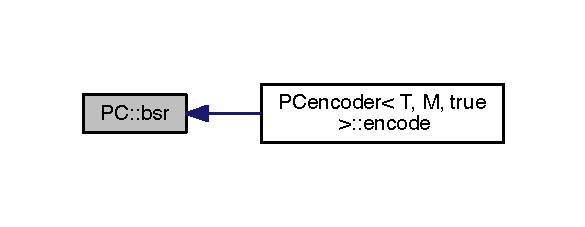
\includegraphics[width=281pt]{da/de6/namespace_p_c_a724d3cf3721b4d3f02a0af4a68e0acea_icgraph}
\end{center}
\end{figure}



\chapter{Class Documentation}
\hypertarget{struct__header}{}\section{\+\_\+header Struct Reference}
\label{struct__header}\index{\+\_\+header@{\+\_\+header}}


{\ttfamily \#include $<$Z\+Bin\+Dumper\+\_\+\+M\+P\+I.\+h$>$}

\subsection*{Public Attributes}
\begin{DoxyCompactItemize}
\item 
long \hyperlink{struct__header_a246169d2b9ff16a190fdf4ce59cd34c6}{offset} \mbox{[}8\mbox{]}
\item 
long \hyperlink{struct__header_a0ddee6f91054f1f35cad4311f1556491}{size} \mbox{[}8\mbox{]}
\end{DoxyCompactItemize}


\subsection{Member Data Documentation}
\hypertarget{struct__header_a246169d2b9ff16a190fdf4ce59cd34c6}{}\index{\+\_\+header@{\+\_\+header}!offset@{offset}}
\index{offset@{offset}!\+\_\+header@{\+\_\+header}}
\subsubsection[{offset}]{\setlength{\rightskip}{0pt plus 5cm}long \+\_\+header\+::offset\mbox{[}8\mbox{]}}\label{struct__header_a246169d2b9ff16a190fdf4ce59cd34c6}
\hypertarget{struct__header_a0ddee6f91054f1f35cad4311f1556491}{}\index{\+\_\+header@{\+\_\+header}!size@{size}}
\index{size@{size}!\+\_\+header@{\+\_\+header}}
\subsubsection[{size}]{\setlength{\rightskip}{0pt plus 5cm}long \+\_\+header\+::size\mbox{[}8\mbox{]}}\label{struct__header_a0ddee6f91054f1f35cad4311f1556491}


The documentation for this struct was generated from the following file\+:\begin{DoxyCompactItemize}
\item 
/\+Users/cconti/\+Desktop/\+Mounts/\+Brutus\+Home/\+Cubism\+U\+P\+\_\+2\+D/\+Cubism/\hyperlink{_z_bin_dumper___m_p_i_8h}{Z\+Bin\+Dumper\+\_\+\+M\+P\+I.\+h}\end{DoxyCompactItemize}

\hypertarget{class_argument_parser}{}\section{Argument\+Parser Class Reference}
\label{class_argument_parser}\index{Argument\+Parser@{Argument\+Parser}}


{\ttfamily \#include $<$Argument\+Parser.\+h$>$}

\subsection*{Public Member Functions}
\begin{DoxyCompactItemize}
\item 
\hyperlink{class_value}{Value} \hyperlink{class_argument_parser_acca583e2f4ed0d0eea39df89e03977ee}{operator()} (const \hyperlink{testfpzip_8cpp_a984bb8e04129c4268bd6ff36a50c9fa4}{string} arg)
\item 
bool \hyperlink{class_argument_parser_adf986abe5c47699a651ee939e198407d}{check} (const \hyperlink{testfpzip_8cpp_a984bb8e04129c4268bd6ff36a50c9fa4}{string} arg) const 
\item 
\hyperlink{class_argument_parser_a1355ae6f318c765d406d4ea600d2ea62}{Argument\+Parser} (const int argc, const char $\ast$$\ast$argv)
\item 
int \hyperlink{class_argument_parser_a778f72cb66634cea1a93446c4a0bc428}{getargc} () const 
\item 
const char $\ast$$\ast$ \hyperlink{class_argument_parser_aa20c2b84e7f77cfd65e315b8291fe342}{getargv} () const 
\item 
void \hyperlink{class_argument_parser_af30fc2364f2e0cf72e9ce17bf30fd645}{set\+\_\+strict\+\_\+mode} ()
\item 
void \hyperlink{class_argument_parser_a47b9bd39a2587221398c6785560072f8}{unset\+\_\+strict\+\_\+mode} ()
\item 
void \hyperlink{class_argument_parser_a6aaf4cd8c288d4de96aefdd5299a4f59}{mute} ()
\item 
void \hyperlink{class_argument_parser_acafcfe7dfe91ced9a020a65979bf03d9}{loud} ()
\item 
void \hyperlink{class_argument_parser_a10793f42b5c6bbb358d2929b2dc09c0f}{save\+\_\+options} (\hyperlink{testfpzip_8cpp_a984bb8e04129c4268bd6ff36a50c9fa4}{string} path=\char`\"{}.\char`\"{})
\end{DoxyCompactItemize}


\subsection{Constructor \& Destructor Documentation}
\hypertarget{class_argument_parser_a1355ae6f318c765d406d4ea600d2ea62}{}\index{Argument\+Parser@{Argument\+Parser}!Argument\+Parser@{Argument\+Parser}}
\index{Argument\+Parser@{Argument\+Parser}!Argument\+Parser@{Argument\+Parser}}
\subsubsection[{Argument\+Parser}]{\setlength{\rightskip}{0pt plus 5cm}Argument\+Parser\+::\+Argument\+Parser (
\begin{DoxyParamCaption}
\item[{const int}]{argc, }
\item[{const char $\ast$$\ast$}]{argv}
\end{DoxyParamCaption}
)\hspace{0.3cm}{\ttfamily [inline]}}\label{class_argument_parser_a1355ae6f318c765d406d4ea600d2ea62}


\subsection{Member Function Documentation}
\hypertarget{class_argument_parser_adf986abe5c47699a651ee939e198407d}{}\index{Argument\+Parser@{Argument\+Parser}!check@{check}}
\index{check@{check}!Argument\+Parser@{Argument\+Parser}}
\subsubsection[{check}]{\setlength{\rightskip}{0pt plus 5cm}bool Argument\+Parser\+::check (
\begin{DoxyParamCaption}
\item[{const {\bf string}}]{arg}
\end{DoxyParamCaption}
) const\hspace{0.3cm}{\ttfamily [inline]}}\label{class_argument_parser_adf986abe5c47699a651ee939e198407d}
\hypertarget{class_argument_parser_a778f72cb66634cea1a93446c4a0bc428}{}\index{Argument\+Parser@{Argument\+Parser}!getargc@{getargc}}
\index{getargc@{getargc}!Argument\+Parser@{Argument\+Parser}}
\subsubsection[{getargc}]{\setlength{\rightskip}{0pt plus 5cm}int Argument\+Parser\+::getargc (
\begin{DoxyParamCaption}
{}
\end{DoxyParamCaption}
) const\hspace{0.3cm}{\ttfamily [inline]}}\label{class_argument_parser_a778f72cb66634cea1a93446c4a0bc428}
\hypertarget{class_argument_parser_aa20c2b84e7f77cfd65e315b8291fe342}{}\index{Argument\+Parser@{Argument\+Parser}!getargv@{getargv}}
\index{getargv@{getargv}!Argument\+Parser@{Argument\+Parser}}
\subsubsection[{getargv}]{\setlength{\rightskip}{0pt plus 5cm}const char$\ast$$\ast$ Argument\+Parser\+::getargv (
\begin{DoxyParamCaption}
{}
\end{DoxyParamCaption}
) const\hspace{0.3cm}{\ttfamily [inline]}}\label{class_argument_parser_aa20c2b84e7f77cfd65e315b8291fe342}
\hypertarget{class_argument_parser_acafcfe7dfe91ced9a020a65979bf03d9}{}\index{Argument\+Parser@{Argument\+Parser}!loud@{loud}}
\index{loud@{loud}!Argument\+Parser@{Argument\+Parser}}
\subsubsection[{loud}]{\setlength{\rightskip}{0pt plus 5cm}void Argument\+Parser\+::loud (
\begin{DoxyParamCaption}
{}
\end{DoxyParamCaption}
)\hspace{0.3cm}{\ttfamily [inline]}}\label{class_argument_parser_acafcfe7dfe91ced9a020a65979bf03d9}
\hypertarget{class_argument_parser_a6aaf4cd8c288d4de96aefdd5299a4f59}{}\index{Argument\+Parser@{Argument\+Parser}!mute@{mute}}
\index{mute@{mute}!Argument\+Parser@{Argument\+Parser}}
\subsubsection[{mute}]{\setlength{\rightskip}{0pt plus 5cm}void Argument\+Parser\+::mute (
\begin{DoxyParamCaption}
{}
\end{DoxyParamCaption}
)\hspace{0.3cm}{\ttfamily [inline]}}\label{class_argument_parser_a6aaf4cd8c288d4de96aefdd5299a4f59}
\hypertarget{class_argument_parser_acca583e2f4ed0d0eea39df89e03977ee}{}\index{Argument\+Parser@{Argument\+Parser}!operator()@{operator()}}
\index{operator()@{operator()}!Argument\+Parser@{Argument\+Parser}}
\subsubsection[{operator()}]{\setlength{\rightskip}{0pt plus 5cm}{\bf Value} Argument\+Parser\+::operator() (
\begin{DoxyParamCaption}
\item[{const {\bf string}}]{arg}
\end{DoxyParamCaption}
)\hspace{0.3cm}{\ttfamily [inline]}}\label{class_argument_parser_acca583e2f4ed0d0eea39df89e03977ee}
\hypertarget{class_argument_parser_a10793f42b5c6bbb358d2929b2dc09c0f}{}\index{Argument\+Parser@{Argument\+Parser}!save\+\_\+options@{save\+\_\+options}}
\index{save\+\_\+options@{save\+\_\+options}!Argument\+Parser@{Argument\+Parser}}
\subsubsection[{save\+\_\+options}]{\setlength{\rightskip}{0pt plus 5cm}void Argument\+Parser\+::save\+\_\+options (
\begin{DoxyParamCaption}
\item[{{\bf string}}]{path = {\ttfamily \char`\"{}.\char`\"{}}}
\end{DoxyParamCaption}
)\hspace{0.3cm}{\ttfamily [inline]}}\label{class_argument_parser_a10793f42b5c6bbb358d2929b2dc09c0f}
\hypertarget{class_argument_parser_af30fc2364f2e0cf72e9ce17bf30fd645}{}\index{Argument\+Parser@{Argument\+Parser}!set\+\_\+strict\+\_\+mode@{set\+\_\+strict\+\_\+mode}}
\index{set\+\_\+strict\+\_\+mode@{set\+\_\+strict\+\_\+mode}!Argument\+Parser@{Argument\+Parser}}
\subsubsection[{set\+\_\+strict\+\_\+mode}]{\setlength{\rightskip}{0pt plus 5cm}void Argument\+Parser\+::set\+\_\+strict\+\_\+mode (
\begin{DoxyParamCaption}
{}
\end{DoxyParamCaption}
)\hspace{0.3cm}{\ttfamily [inline]}}\label{class_argument_parser_af30fc2364f2e0cf72e9ce17bf30fd645}


Here is the caller graph for this function\+:\nopagebreak
\begin{figure}[H]
\begin{center}
\leavevmode
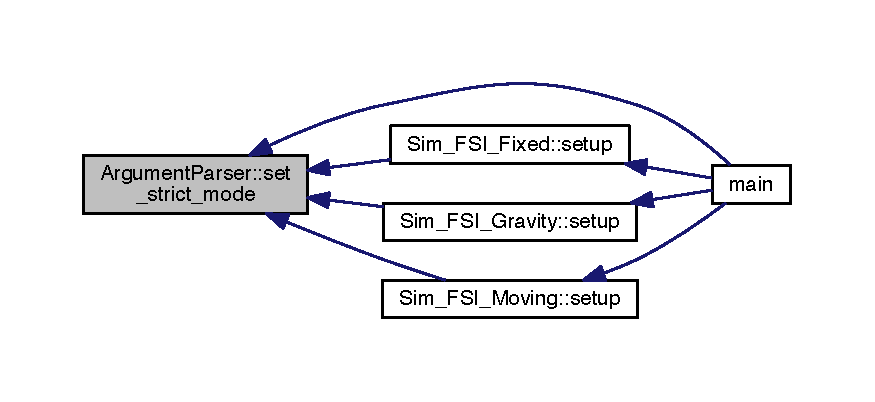
\includegraphics[width=350pt]{d3/d52/class_argument_parser_af30fc2364f2e0cf72e9ce17bf30fd645_icgraph}
\end{center}
\end{figure}


\hypertarget{class_argument_parser_a47b9bd39a2587221398c6785560072f8}{}\index{Argument\+Parser@{Argument\+Parser}!unset\+\_\+strict\+\_\+mode@{unset\+\_\+strict\+\_\+mode}}
\index{unset\+\_\+strict\+\_\+mode@{unset\+\_\+strict\+\_\+mode}!Argument\+Parser@{Argument\+Parser}}
\subsubsection[{unset\+\_\+strict\+\_\+mode}]{\setlength{\rightskip}{0pt plus 5cm}void Argument\+Parser\+::unset\+\_\+strict\+\_\+mode (
\begin{DoxyParamCaption}
{}
\end{DoxyParamCaption}
)\hspace{0.3cm}{\ttfamily [inline]}}\label{class_argument_parser_a47b9bd39a2587221398c6785560072f8}


Here is the caller graph for this function\+:\nopagebreak
\begin{figure}[H]
\begin{center}
\leavevmode
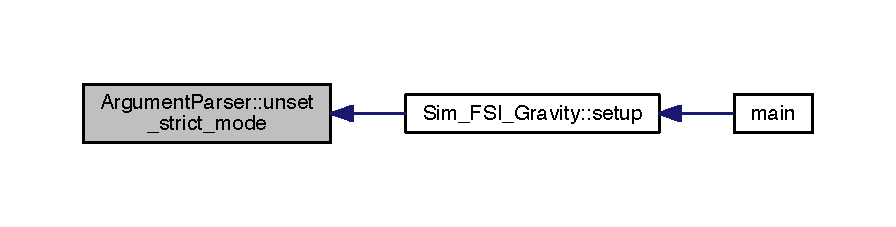
\includegraphics[width=350pt]{d3/d52/class_argument_parser_a47b9bd39a2587221398c6785560072f8_icgraph}
\end{center}
\end{figure}




The documentation for this class was generated from the following file\+:\begin{DoxyCompactItemize}
\item 
/\+Users/cconti/\+Desktop/\+Mounts/\+Brutus\+Home/\+Cubism\+U\+P\+\_\+2\+D/\+Cubism/\hyperlink{_argument_parser_8h}{Argument\+Parser.\+h}\end{DoxyCompactItemize}

\hypertarget{struct_block_info}{}\section{Block\+Info Struct Reference}
\label{struct_block_info}\index{Block\+Info@{Block\+Info}}


{\ttfamily \#include $<$Block\+Info.\+h$>$}

\subsection*{Public Member Functions}
\begin{DoxyCompactItemize}
\item 
{\footnotesize template$<$typename T $>$ }\\void \hyperlink{struct_block_info_abcc226bdb973d09286902ae23f3962fd}{pos} (T p\mbox{[}2\mbox{]}, int ix, int iy) const 
\item 
{\footnotesize template$<$typename T $>$ }\\void \hyperlink{struct_block_info_a803920cf6f3185de720fe789fa59f6cb}{pos} (T p\mbox{[}3\mbox{]}, int ix, int iy, int iz) const 
\item 
\hyperlink{struct_block_info_a02f86d450ef17d29635aa21622b641df}{Block\+Info} (long long I\+D, const int idx\mbox{[}3\mbox{]}, const double \hyperlink{struct_block_info_abcc226bdb973d09286902ae23f3962fd}{pos}\mbox{[}3\mbox{]}, const double spacing, double h\+\_\+gridpoint\+\_\+, void $\ast$ptr=N\+U\+L\+L)
\item 
\hyperlink{struct_block_info_a6b27ee44e1fa4f1b7eddb1f2e9dcaba7}{Block\+Info} ()
\end{DoxyCompactItemize}
\subsection*{Public Attributes}
\begin{DoxyCompactItemize}
\item 
long long \hyperlink{struct_block_info_aff4a50657c14cc550c9e0e3aaaed1a15}{block\+I\+D}
\item 
void $\ast$ \hyperlink{struct_block_info_af3655416c17becfb24a9f475a7b97d23}{ptr\+Block}
\item 
int \hyperlink{struct_block_info_ad32832aaa2dee35464a74abfae741572}{index} \mbox{[}3\mbox{]}
\item 
double \hyperlink{struct_block_info_a8d2d03097cfbffc58d3cc2dee371e4b2}{origin} \mbox{[}3\mbox{]}
\item 
double \hyperlink{struct_block_info_abb250cd39311bd0a840588ff2a6196ad}{h}
\item 
double \hyperlink{struct_block_info_a83bd46701539e64d666206d6501ee3ea}{h\+\_\+gridpoint}
\end{DoxyCompactItemize}


\subsection{Constructor \& Destructor Documentation}
\hypertarget{struct_block_info_a02f86d450ef17d29635aa21622b641df}{}\index{Block\+Info@{Block\+Info}!Block\+Info@{Block\+Info}}
\index{Block\+Info@{Block\+Info}!Block\+Info@{Block\+Info}}
\subsubsection[{Block\+Info}]{\setlength{\rightskip}{0pt plus 5cm}Block\+Info\+::\+Block\+Info (
\begin{DoxyParamCaption}
\item[{long long}]{I\+D, }
\item[{const int}]{idx\mbox{[}3\mbox{]}, }
\item[{const double}]{pos\mbox{[}3\mbox{]}, }
\item[{const double}]{spacing, }
\item[{double}]{h\+\_\+gridpoint\+\_\+, }
\item[{void $\ast$}]{ptr = {\ttfamily NULL}}
\end{DoxyParamCaption}
)\hspace{0.3cm}{\ttfamily [inline]}}\label{struct_block_info_a02f86d450ef17d29635aa21622b641df}
\hypertarget{struct_block_info_a6b27ee44e1fa4f1b7eddb1f2e9dcaba7}{}\index{Block\+Info@{Block\+Info}!Block\+Info@{Block\+Info}}
\index{Block\+Info@{Block\+Info}!Block\+Info@{Block\+Info}}
\subsubsection[{Block\+Info}]{\setlength{\rightskip}{0pt plus 5cm}Block\+Info\+::\+Block\+Info (
\begin{DoxyParamCaption}
{}
\end{DoxyParamCaption}
)\hspace{0.3cm}{\ttfamily [inline]}}\label{struct_block_info_a6b27ee44e1fa4f1b7eddb1f2e9dcaba7}


\subsection{Member Function Documentation}
\hypertarget{struct_block_info_abcc226bdb973d09286902ae23f3962fd}{}\index{Block\+Info@{Block\+Info}!pos@{pos}}
\index{pos@{pos}!Block\+Info@{Block\+Info}}
\subsubsection[{pos}]{\setlength{\rightskip}{0pt plus 5cm}template$<$typename T $>$ void Block\+Info\+::pos (
\begin{DoxyParamCaption}
\item[{T}]{p\mbox{[}2\mbox{]}, }
\item[{int}]{ix, }
\item[{int}]{iy}
\end{DoxyParamCaption}
) const\hspace{0.3cm}{\ttfamily [inline]}}\label{struct_block_info_abcc226bdb973d09286902ae23f3962fd}


Here is the caller graph for this function\+:
\nopagebreak
\begin{figure}[H]
\begin{center}
\leavevmode
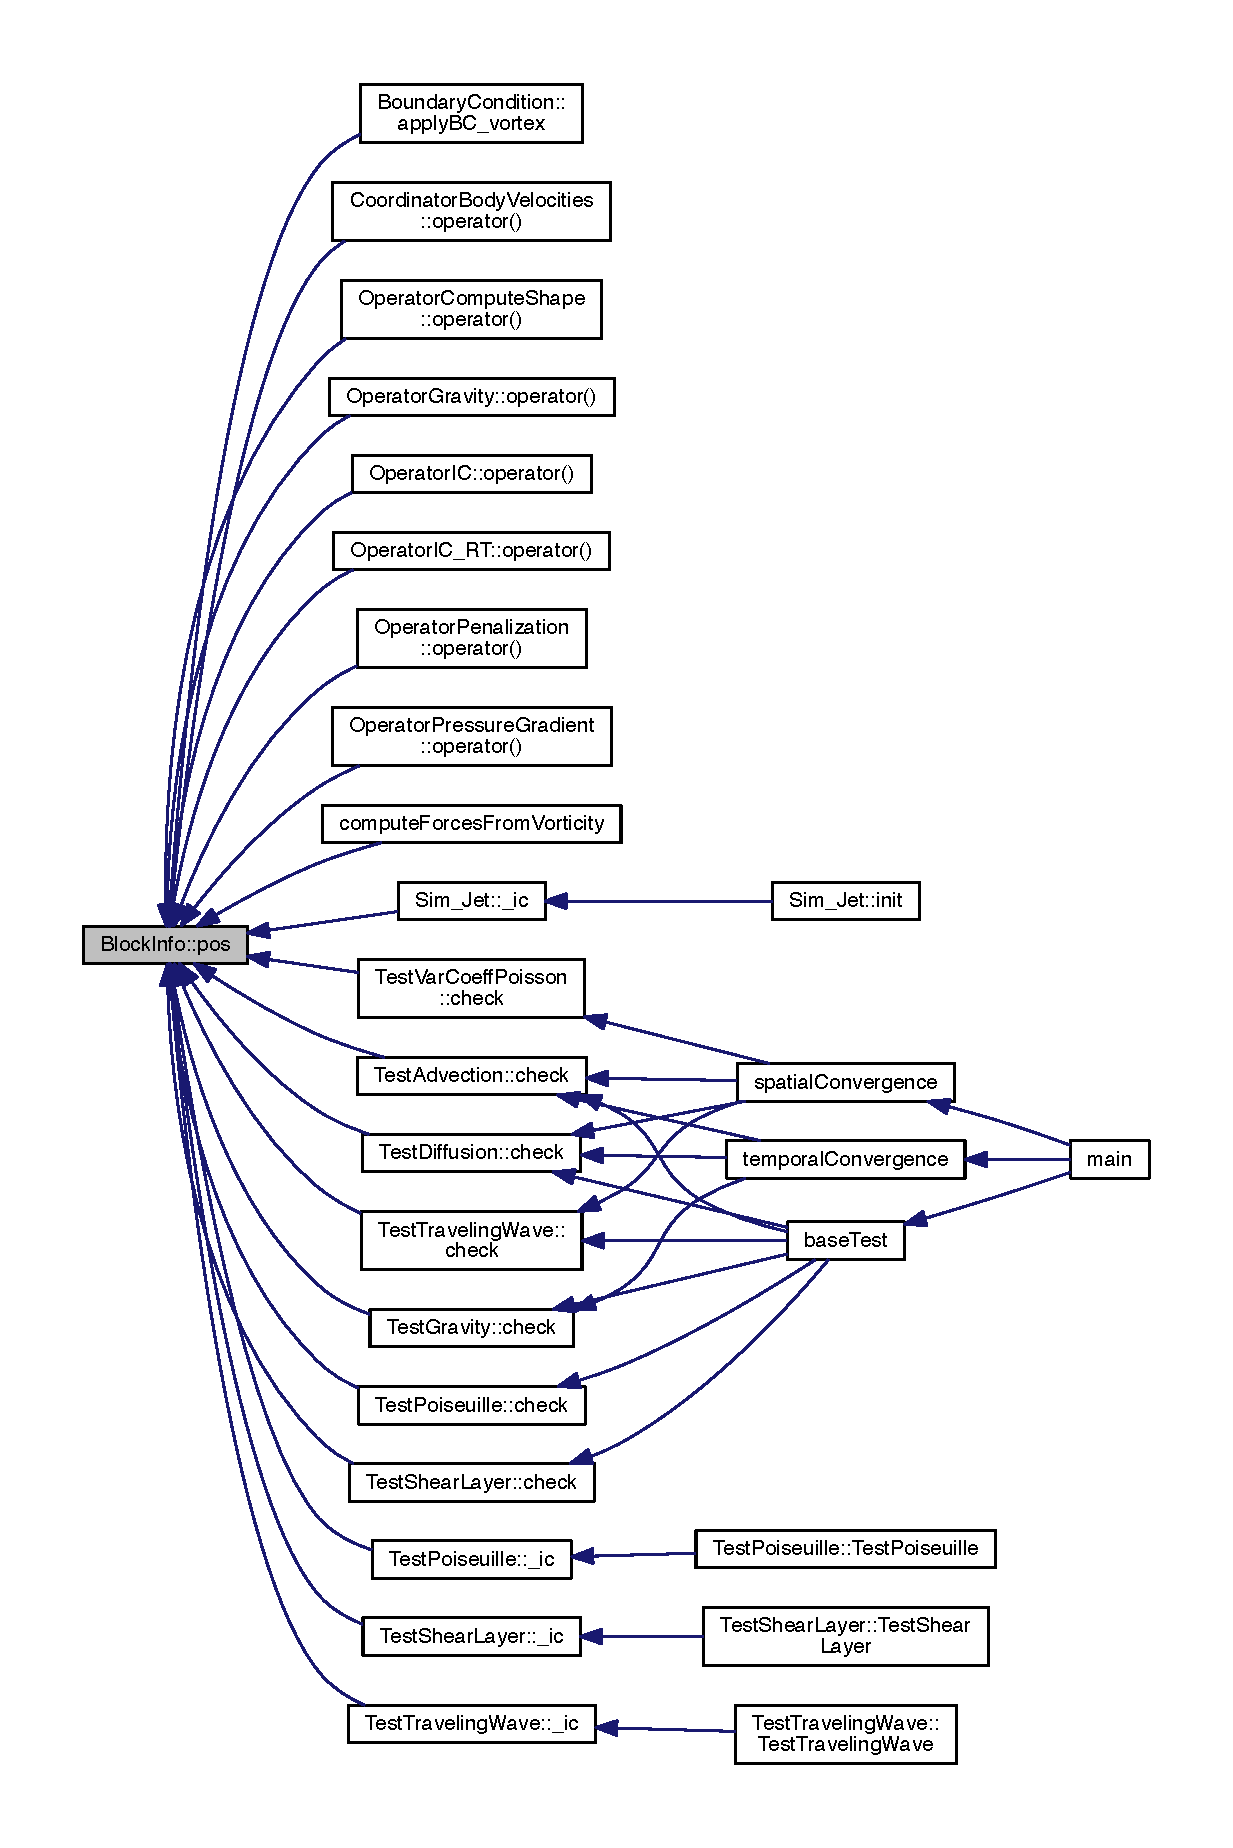
\includegraphics[width=350pt]{d4/ded/struct_block_info_abcc226bdb973d09286902ae23f3962fd_icgraph}
\end{center}
\end{figure}


\hypertarget{struct_block_info_a803920cf6f3185de720fe789fa59f6cb}{}\index{Block\+Info@{Block\+Info}!pos@{pos}}
\index{pos@{pos}!Block\+Info@{Block\+Info}}
\subsubsection[{pos}]{\setlength{\rightskip}{0pt plus 5cm}template$<$typename T $>$ void Block\+Info\+::pos (
\begin{DoxyParamCaption}
\item[{T}]{p\mbox{[}3\mbox{]}, }
\item[{int}]{ix, }
\item[{int}]{iy, }
\item[{int}]{iz}
\end{DoxyParamCaption}
) const\hspace{0.3cm}{\ttfamily [inline]}}\label{struct_block_info_a803920cf6f3185de720fe789fa59f6cb}


\subsection{Member Data Documentation}
\hypertarget{struct_block_info_aff4a50657c14cc550c9e0e3aaaed1a15}{}\index{Block\+Info@{Block\+Info}!block\+I\+D@{block\+I\+D}}
\index{block\+I\+D@{block\+I\+D}!Block\+Info@{Block\+Info}}
\subsubsection[{block\+I\+D}]{\setlength{\rightskip}{0pt plus 5cm}long long Block\+Info\+::block\+I\+D}\label{struct_block_info_aff4a50657c14cc550c9e0e3aaaed1a15}
\hypertarget{struct_block_info_abb250cd39311bd0a840588ff2a6196ad}{}\index{Block\+Info@{Block\+Info}!h@{h}}
\index{h@{h}!Block\+Info@{Block\+Info}}
\subsubsection[{h}]{\setlength{\rightskip}{0pt plus 5cm}double Block\+Info\+::h}\label{struct_block_info_abb250cd39311bd0a840588ff2a6196ad}
\hypertarget{struct_block_info_a83bd46701539e64d666206d6501ee3ea}{}\index{Block\+Info@{Block\+Info}!h\+\_\+gridpoint@{h\+\_\+gridpoint}}
\index{h\+\_\+gridpoint@{h\+\_\+gridpoint}!Block\+Info@{Block\+Info}}
\subsubsection[{h\+\_\+gridpoint}]{\setlength{\rightskip}{0pt plus 5cm}double Block\+Info\+::h\+\_\+gridpoint}\label{struct_block_info_a83bd46701539e64d666206d6501ee3ea}
\hypertarget{struct_block_info_ad32832aaa2dee35464a74abfae741572}{}\index{Block\+Info@{Block\+Info}!index@{index}}
\index{index@{index}!Block\+Info@{Block\+Info}}
\subsubsection[{index}]{\setlength{\rightskip}{0pt plus 5cm}int Block\+Info\+::index\mbox{[}3\mbox{]}}\label{struct_block_info_ad32832aaa2dee35464a74abfae741572}
\hypertarget{struct_block_info_a8d2d03097cfbffc58d3cc2dee371e4b2}{}\index{Block\+Info@{Block\+Info}!origin@{origin}}
\index{origin@{origin}!Block\+Info@{Block\+Info}}
\subsubsection[{origin}]{\setlength{\rightskip}{0pt plus 5cm}double Block\+Info\+::origin\mbox{[}3\mbox{]}}\label{struct_block_info_a8d2d03097cfbffc58d3cc2dee371e4b2}
\hypertarget{struct_block_info_af3655416c17becfb24a9f475a7b97d23}{}\index{Block\+Info@{Block\+Info}!ptr\+Block@{ptr\+Block}}
\index{ptr\+Block@{ptr\+Block}!Block\+Info@{Block\+Info}}
\subsubsection[{ptr\+Block}]{\setlength{\rightskip}{0pt plus 5cm}void$\ast$ Block\+Info\+::ptr\+Block}\label{struct_block_info_af3655416c17becfb24a9f475a7b97d23}


The documentation for this struct was generated from the following file\+:\begin{DoxyCompactItemize}
\item 
/\+Users/cconti/\+Desktop/\+Mounts/\+Brutus\+Home/\+Cubism\+U\+P\+\_\+2\+D/\+Cubism/\hyperlink{_block_info_8h}{Block\+Info.\+h}\end{DoxyCompactItemize}

\hypertarget{class_block_lab}{}\section{Block\+Lab$<$ T\+Block, allocator, Element\+Type\+T $>$ Class Template Reference}
\label{class_block_lab}\index{Block\+Lab$<$ T\+Block, allocator, Element\+Type\+T $>$@{Block\+Lab$<$ T\+Block, allocator, Element\+Type\+T $>$}}


{\ttfamily \#include $<$Block\+Lab.\+h$>$}



Collaboration diagram for Block\+Lab$<$ T\+Block, allocator, Element\+Type\+T $>$\+:\nopagebreak
\begin{figure}[H]
\begin{center}
\leavevmode
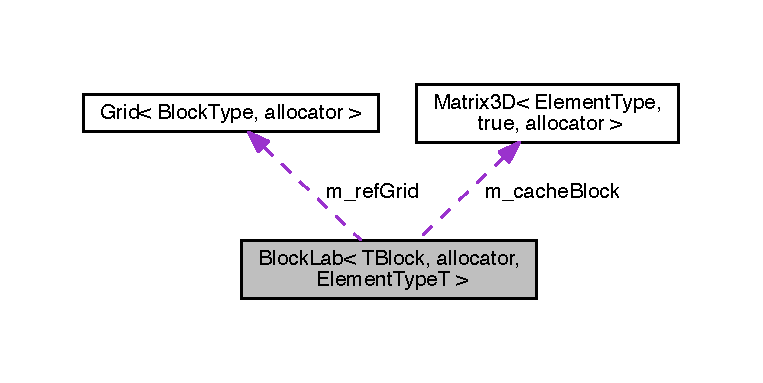
\includegraphics[width=350pt]{da/daa/class_block_lab__coll__graph}
\end{center}
\end{figure}
\subsection*{Public Types}
\begin{DoxyCompactItemize}
\item 
typedef Element\+Type\+T \hyperlink{class_block_lab_accdcd2d5e815a8497e5ef9ae884da6b6}{Element\+Type}
\end{DoxyCompactItemize}
\subsection*{Public Member Functions}
\begin{DoxyCompactItemize}
\item 
\hyperlink{class_block_lab_a0cb8aec5f42c4b1860be8aa218660087}{Block\+Lab} ()
\item 
virtual bool \hyperlink{class_block_lab_aaf6e3ab940c5c3cf7463bad112527f98}{is\+\_\+xperiodic} ()
\item 
virtual bool \hyperlink{class_block_lab_a5455e54c8e874ee9da6159ea0d1651ed}{is\+\_\+yperiodic} ()
\item 
virtual bool \hyperlink{class_block_lab_a0fd3a720fb3f2f76845ff4323e89bb91}{is\+\_\+zperiodic} ()
\item 
\hyperlink{class_block_lab_a083218471f59c32fccc335759734667d}{$\sim$\+Block\+Lab} ()
\item 
{\footnotesize template$<$int dim$>$ }\\int \hyperlink{class_block_lab_aa45e40066bececd40de75c238c346e79}{get\+Actual\+Size} () const 
\item 
\hyperlink{class_block_lab_accdcd2d5e815a8497e5ef9ae884da6b6}{Element\+Type} $\ast$ \hyperlink{class_block_lab_a4dd07a50f8766b29717b9326e67a9fcd}{get\+Buffer} () const 
\item 
void \hyperlink{class_block_lab_ad529f8c851da336419ad63c25ba76429}{prepare} (\hyperlink{class_grid}{Grid}$<$ \hyperlink{class_block_lab_a745b3c9ac17f6743d11a7085196981a0}{Block\+Type}, allocator $>$ \&grid, int start\+X, int end\+X, int start\+Y, int end\+Y, int start\+Z, int end\+Z, const bool \hyperlink{class_block_lab_ade306bb6935a0ead765444534c2e05db}{istensorial})
\item 
void \hyperlink{class_block_lab_ac6236e1c94d13fa1025c8253b9855a04}{prepare} (\hyperlink{class_grid}{Grid}$<$ \hyperlink{class_block_lab_a745b3c9ac17f6743d11a7085196981a0}{Block\+Type}, allocator $>$ \&grid, const int stencil\+\_\+start\mbox{[}3\mbox{]}, const int stencil\+\_\+end\mbox{[}3\mbox{]}, const bool \hyperlink{class_block_lab_ade306bb6935a0ead765444534c2e05db}{istensorial})
\item 
void \hyperlink{class_block_lab_aefd27fed8fbb1d3d60fe1457ae90f248}{load} (const \hyperlink{struct_block_info}{Block\+Info} \&info, const \hyperlink{_h_d_f5_dumper_8h_a445a5f0e2a34c9d97d69a3c2d1957907}{Real} t=0, const bool applybc=true)
\item 
\hyperlink{class_block_lab_accdcd2d5e815a8497e5ef9ae884da6b6}{Element\+Type} \& \hyperlink{class_block_lab_abd79a09ab5b54cf04bfe25c125ea1edf}{operator()} (int ix, int iy=0, int iz=0)
\item 
const \hyperlink{class_block_lab_accdcd2d5e815a8497e5ef9ae884da6b6}{Element\+Type} \& \hyperlink{class_block_lab_a3e06d4124f7d69923b4ee6345c105cfc}{read} (int ix, int iy=0, int iz=0) const 
\end{DoxyCompactItemize}
\subsection*{Protected Types}
\begin{DoxyCompactItemize}
\item 
enum \hyperlink{class_block_lab_ad3a1e6e1a1002fb812d6853c8ac1ec9e}{e\+Block\+Lab\+\_\+\+State} \{ \hyperlink{class_block_lab_ad3a1e6e1a1002fb812d6853c8ac1ec9ea6c1a64be2e953c6093dab00aab32fe00}{e\+M\+R\+A\+G\+Block\+Lab\+\_\+\+Prepared}, 
\hyperlink{class_block_lab_ad3a1e6e1a1002fb812d6853c8ac1ec9eadaaa507dbe601b991a383e6a0701a09c}{e\+M\+R\+A\+G\+Block\+Lab\+\_\+\+Loaded}, 
\hyperlink{class_block_lab_ad3a1e6e1a1002fb812d6853c8ac1ec9ead9471f6585bd7cf7ddc9edad96e67362}{e\+M\+R\+A\+G\+Block\+Lab\+\_\+\+Uninitialized}
 \}
\item 
typedef T\+Block \hyperlink{class_block_lab_a745b3c9ac17f6743d11a7085196981a0}{Block\+Type}
\item 
typedef Block\+Type\+::\+Element\+Type \hyperlink{class_block_lab_ad547d74881a0d226a849e2051af6b26b}{Element\+Type\+Block}
\end{DoxyCompactItemize}
\subsection*{Protected Member Functions}
\begin{DoxyCompactItemize}
\item 
virtual void \hyperlink{class_block_lab_a669ac139b57be4967e5f43bc649a8520}{\+\_\+apply\+\_\+bc} (const \hyperlink{struct_block_info}{Block\+Info} \&info, const \hyperlink{_h_d_f5_dumper_8h_a445a5f0e2a34c9d97d69a3c2d1957907}{Real} t=0)
\item 
{\footnotesize template$<$typename T $>$ }\\void \hyperlink{class_block_lab_ab23c907953858c8b393a9910ecf5b1cf}{\+\_\+release} (T $\ast$\&t)
\end{DoxyCompactItemize}
\subsection*{Protected Attributes}
\begin{DoxyCompactItemize}
\item 
\hyperlink{class_block_lab_ad3a1e6e1a1002fb812d6853c8ac1ec9e}{e\+Block\+Lab\+\_\+\+State} \hyperlink{class_block_lab_a0e11603d73ab4923e1d9033edccdb572}{m\+\_\+state}
\item 
\hyperlink{class_matrix3_d}{Matrix3\+D}$<$ \hyperlink{class_block_lab_accdcd2d5e815a8497e5ef9ae884da6b6}{Element\+Type}, true, allocator $>$ $\ast$ \hyperlink{class_block_lab_aa6a4c4e00a9bb5ca5780d820b146485b}{m\+\_\+cache\+Block}
\item 
int \hyperlink{class_block_lab_a8ac6690f98ba84346a74b5b95c3afb2b}{m\+\_\+stencil\+Start} \mbox{[}3\mbox{]}
\item 
int \hyperlink{class_block_lab_a46fee08b49b11be489c71f726e258cc9}{m\+\_\+stencil\+End} \mbox{[}3\mbox{]}
\item 
int \hyperlink{class_block_lab_abcd7367c6f45124d3202c8da5043ac93}{N\+X}
\item 
int \hyperlink{class_block_lab_aaa1e748664ebb6b4fc7c47cf30a445db}{N\+Y}
\item 
int \hyperlink{class_block_lab_acdd7f4e2489d31da6a2a76099807a7c5}{N\+Z}
\item 
bool \hyperlink{class_block_lab_ade306bb6935a0ead765444534c2e05db}{istensorial}
\item 
const \hyperlink{class_grid}{Grid}$<$ \hyperlink{class_block_lab_a745b3c9ac17f6743d11a7085196981a0}{Block\+Type}, allocator $>$ $\ast$ \hyperlink{class_block_lab_acccfe85f166f20526118fce09b28fb04}{m\+\_\+ref\+Grid}
\end{DoxyCompactItemize}


\subsection{Detailed Description}
\subsubsection*{template$<$typename T\+Block, template$<$ typename X $>$ class allocator = std\+::allocator, typename Element\+Type\+T = typename T\+Block\+::\+Element\+Type$>$class Block\+Lab$<$ T\+Block, allocator, Element\+Type\+T $>$}

Working copy of Block + Ghosts. Data of original block is copied (!) here. So when changing something in the lab we are not changing the original data. Requirements\+:
\begin{DoxyItemize}
\item Concepts\+::\+Block\+Lab\+Element\+Type$<$\+Element\+Type\+T$>$
\item Concepts\+::\+Castable$<$typename Block\+Type\+::\+Element\+Type, Element\+Type\+T$>$ 
\end{DoxyItemize}

\subsection{Member Typedef Documentation}
\hypertarget{class_block_lab_a745b3c9ac17f6743d11a7085196981a0}{}\index{Block\+Lab@{Block\+Lab}!Block\+Type@{Block\+Type}}
\index{Block\+Type@{Block\+Type}!Block\+Lab@{Block\+Lab}}
\subsubsection[{Block\+Type}]{\setlength{\rightskip}{0pt plus 5cm}template$<$typename T\+Block, template$<$ typename X $>$ class allocator = std\+::allocator, typename Element\+Type\+T = typename T\+Block\+::\+Element\+Type$>$ typedef T\+Block {\bf Block\+Lab}$<$ T\+Block, allocator, Element\+Type\+T $>$\+::{\bf Block\+Type}\hspace{0.3cm}{\ttfamily [protected]}}\label{class_block_lab_a745b3c9ac17f6743d11a7085196981a0}
\hypertarget{class_block_lab_accdcd2d5e815a8497e5ef9ae884da6b6}{}\index{Block\+Lab@{Block\+Lab}!Element\+Type@{Element\+Type}}
\index{Element\+Type@{Element\+Type}!Block\+Lab@{Block\+Lab}}
\subsubsection[{Element\+Type}]{\setlength{\rightskip}{0pt plus 5cm}template$<$typename T\+Block, template$<$ typename X $>$ class allocator = std\+::allocator, typename Element\+Type\+T = typename T\+Block\+::\+Element\+Type$>$ typedef Element\+Type\+T {\bf Block\+Lab}$<$ T\+Block, allocator, Element\+Type\+T $>$\+::{\bf Element\+Type}}\label{class_block_lab_accdcd2d5e815a8497e5ef9ae884da6b6}
\hypertarget{class_block_lab_ad547d74881a0d226a849e2051af6b26b}{}\index{Block\+Lab@{Block\+Lab}!Element\+Type\+Block@{Element\+Type\+Block}}
\index{Element\+Type\+Block@{Element\+Type\+Block}!Block\+Lab@{Block\+Lab}}
\subsubsection[{Element\+Type\+Block}]{\setlength{\rightskip}{0pt plus 5cm}template$<$typename T\+Block, template$<$ typename X $>$ class allocator = std\+::allocator, typename Element\+Type\+T = typename T\+Block\+::\+Element\+Type$>$ typedef Block\+Type\+::\+Element\+Type {\bf Block\+Lab}$<$ T\+Block, allocator, Element\+Type\+T $>$\+::{\bf Element\+Type\+Block}\hspace{0.3cm}{\ttfamily [protected]}}\label{class_block_lab_ad547d74881a0d226a849e2051af6b26b}


\subsection{Member Enumeration Documentation}
\hypertarget{class_block_lab_ad3a1e6e1a1002fb812d6853c8ac1ec9e}{}\index{Block\+Lab@{Block\+Lab}!e\+Block\+Lab\+\_\+\+State@{e\+Block\+Lab\+\_\+\+State}}
\index{e\+Block\+Lab\+\_\+\+State@{e\+Block\+Lab\+\_\+\+State}!Block\+Lab@{Block\+Lab}}
\subsubsection[{e\+Block\+Lab\+\_\+\+State}]{\setlength{\rightskip}{0pt plus 5cm}template$<$typename T\+Block, template$<$ typename X $>$ class allocator = std\+::allocator, typename Element\+Type\+T = typename T\+Block\+::\+Element\+Type$>$ enum {\bf Block\+Lab\+::e\+Block\+Lab\+\_\+\+State}\hspace{0.3cm}{\ttfamily [protected]}}\label{class_block_lab_ad3a1e6e1a1002fb812d6853c8ac1ec9e}
\begin{Desc}
\item[Enumerator]\par
\begin{description}
\index{e\+M\+R\+A\+G\+Block\+Lab\+\_\+\+Prepared@{e\+M\+R\+A\+G\+Block\+Lab\+\_\+\+Prepared}!Block\+Lab@{Block\+Lab}}\index{Block\+Lab@{Block\+Lab}!e\+M\+R\+A\+G\+Block\+Lab\+\_\+\+Prepared@{e\+M\+R\+A\+G\+Block\+Lab\+\_\+\+Prepared}}\item[{\em 
\hypertarget{class_block_lab_ad3a1e6e1a1002fb812d6853c8ac1ec9ea6c1a64be2e953c6093dab00aab32fe00}{}e\+M\+R\+A\+G\+Block\+Lab\+\_\+\+Prepared\label{class_block_lab_ad3a1e6e1a1002fb812d6853c8ac1ec9ea6c1a64be2e953c6093dab00aab32fe00}
}]\index{e\+M\+R\+A\+G\+Block\+Lab\+\_\+\+Loaded@{e\+M\+R\+A\+G\+Block\+Lab\+\_\+\+Loaded}!Block\+Lab@{Block\+Lab}}\index{Block\+Lab@{Block\+Lab}!e\+M\+R\+A\+G\+Block\+Lab\+\_\+\+Loaded@{e\+M\+R\+A\+G\+Block\+Lab\+\_\+\+Loaded}}\item[{\em 
\hypertarget{class_block_lab_ad3a1e6e1a1002fb812d6853c8ac1ec9eadaaa507dbe601b991a383e6a0701a09c}{}e\+M\+R\+A\+G\+Block\+Lab\+\_\+\+Loaded\label{class_block_lab_ad3a1e6e1a1002fb812d6853c8ac1ec9eadaaa507dbe601b991a383e6a0701a09c}
}]\index{e\+M\+R\+A\+G\+Block\+Lab\+\_\+\+Uninitialized@{e\+M\+R\+A\+G\+Block\+Lab\+\_\+\+Uninitialized}!Block\+Lab@{Block\+Lab}}\index{Block\+Lab@{Block\+Lab}!e\+M\+R\+A\+G\+Block\+Lab\+\_\+\+Uninitialized@{e\+M\+R\+A\+G\+Block\+Lab\+\_\+\+Uninitialized}}\item[{\em 
\hypertarget{class_block_lab_ad3a1e6e1a1002fb812d6853c8ac1ec9ead9471f6585bd7cf7ddc9edad96e67362}{}e\+M\+R\+A\+G\+Block\+Lab\+\_\+\+Uninitialized\label{class_block_lab_ad3a1e6e1a1002fb812d6853c8ac1ec9ead9471f6585bd7cf7ddc9edad96e67362}
}]\end{description}
\end{Desc}


\subsection{Constructor \& Destructor Documentation}
\hypertarget{class_block_lab_a0cb8aec5f42c4b1860be8aa218660087}{}\index{Block\+Lab@{Block\+Lab}!Block\+Lab@{Block\+Lab}}
\index{Block\+Lab@{Block\+Lab}!Block\+Lab@{Block\+Lab}}
\subsubsection[{Block\+Lab}]{\setlength{\rightskip}{0pt plus 5cm}template$<$typename T\+Block, template$<$ typename X $>$ class allocator = std\+::allocator, typename Element\+Type\+T = typename T\+Block\+::\+Element\+Type$>$ {\bf Block\+Lab}$<$ T\+Block, allocator, Element\+Type\+T $>$\+::{\bf Block\+Lab} (
\begin{DoxyParamCaption}
{}
\end{DoxyParamCaption}
)\hspace{0.3cm}{\ttfamily [inline]}}\label{class_block_lab_a0cb8aec5f42c4b1860be8aa218660087}
\hypertarget{class_block_lab_a083218471f59c32fccc335759734667d}{}\index{Block\+Lab@{Block\+Lab}!````~Block\+Lab@{$\sim$\+Block\+Lab}}
\index{````~Block\+Lab@{$\sim$\+Block\+Lab}!Block\+Lab@{Block\+Lab}}
\subsubsection[{$\sim$\+Block\+Lab}]{\setlength{\rightskip}{0pt plus 5cm}template$<$typename T\+Block, template$<$ typename X $>$ class allocator = std\+::allocator, typename Element\+Type\+T = typename T\+Block\+::\+Element\+Type$>$ {\bf Block\+Lab}$<$ T\+Block, allocator, Element\+Type\+T $>$\+::$\sim${\bf Block\+Lab} (
\begin{DoxyParamCaption}
{}
\end{DoxyParamCaption}
)\hspace{0.3cm}{\ttfamily [inline]}}\label{class_block_lab_a083218471f59c32fccc335759734667d}


\subsection{Member Function Documentation}
\hypertarget{class_block_lab_a669ac139b57be4967e5f43bc649a8520}{}\index{Block\+Lab@{Block\+Lab}!\+\_\+apply\+\_\+bc@{\+\_\+apply\+\_\+bc}}
\index{\+\_\+apply\+\_\+bc@{\+\_\+apply\+\_\+bc}!Block\+Lab@{Block\+Lab}}
\subsubsection[{\+\_\+apply\+\_\+bc}]{\setlength{\rightskip}{0pt plus 5cm}template$<$typename T\+Block, template$<$ typename X $>$ class allocator = std\+::allocator, typename Element\+Type\+T = typename T\+Block\+::\+Element\+Type$>$ virtual void {\bf Block\+Lab}$<$ T\+Block, allocator, Element\+Type\+T $>$\+::\+\_\+apply\+\_\+bc (
\begin{DoxyParamCaption}
\item[{const {\bf Block\+Info} \&}]{info, }
\item[{const {\bf Real}}]{t = {\ttfamily 0}}
\end{DoxyParamCaption}
)\hspace{0.3cm}{\ttfamily [inline]}, {\ttfamily [protected]}, {\ttfamily [virtual]}}\label{class_block_lab_a669ac139b57be4967e5f43bc649a8520}


Reimplemented in \hyperlink{class_block_lab_box_adfd9b3d46062be59f03d0c1df79db81d}{Block\+Lab\+Box$<$ Block\+Type, allocator $>$}, \hyperlink{class_block_lab_neumann_a65cd80126a426fa2aa098910fd189793}{Block\+Lab\+Neumann$<$ Block\+Type, allocator $>$}, and \hyperlink{class_block_lab_dirichlet_ae05580142a8ddb65c42fd92063355609}{Block\+Lab\+Dirichlet$<$ Block\+Type, allocator $>$}.



Here is the caller graph for this function\+:\nopagebreak
\begin{figure}[H]
\begin{center}
\leavevmode
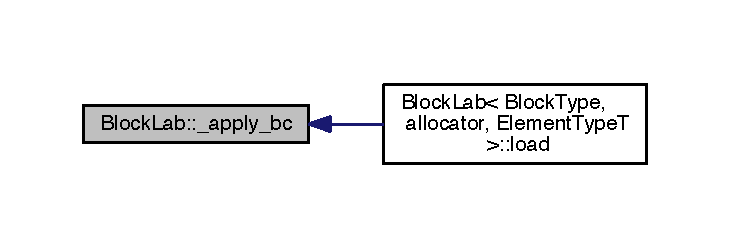
\includegraphics[width=350pt]{d7/d95/class_block_lab_a669ac139b57be4967e5f43bc649a8520_icgraph}
\end{center}
\end{figure}


\hypertarget{class_block_lab_ab23c907953858c8b393a9910ecf5b1cf}{}\index{Block\+Lab@{Block\+Lab}!\+\_\+release@{\+\_\+release}}
\index{\+\_\+release@{\+\_\+release}!Block\+Lab@{Block\+Lab}}
\subsubsection[{\+\_\+release}]{\setlength{\rightskip}{0pt plus 5cm}template$<$typename T\+Block, template$<$ typename X $>$ class allocator = std\+::allocator, typename Element\+Type\+T = typename T\+Block\+::\+Element\+Type$>$ template$<$typename T $>$ void {\bf Block\+Lab}$<$ T\+Block, allocator, Element\+Type\+T $>$\+::\+\_\+release (
\begin{DoxyParamCaption}
\item[{T $\ast$\&}]{t}
\end{DoxyParamCaption}
)\hspace{0.3cm}{\ttfamily [inline]}, {\ttfamily [protected]}}\label{class_block_lab_ab23c907953858c8b393a9910ecf5b1cf}


Here is the caller graph for this function\+:\nopagebreak
\begin{figure}[H]
\begin{center}
\leavevmode
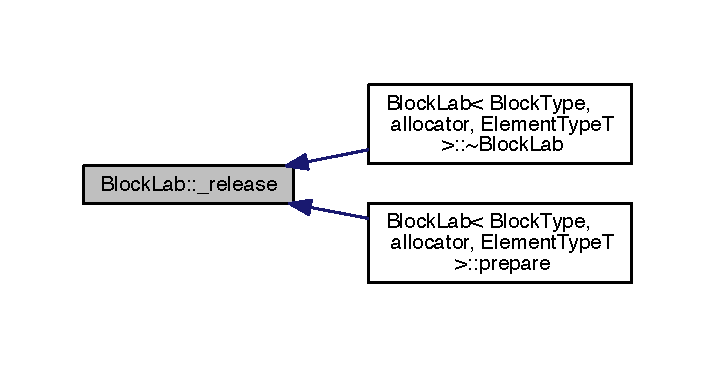
\includegraphics[width=343pt]{d7/d95/class_block_lab_ab23c907953858c8b393a9910ecf5b1cf_icgraph}
\end{center}
\end{figure}


\hypertarget{class_block_lab_aa45e40066bececd40de75c238c346e79}{}\index{Block\+Lab@{Block\+Lab}!get\+Actual\+Size@{get\+Actual\+Size}}
\index{get\+Actual\+Size@{get\+Actual\+Size}!Block\+Lab@{Block\+Lab}}
\subsubsection[{get\+Actual\+Size}]{\setlength{\rightskip}{0pt plus 5cm}template$<$typename T\+Block, template$<$ typename X $>$ class allocator = std\+::allocator, typename Element\+Type\+T = typename T\+Block\+::\+Element\+Type$>$ template$<$int dim$>$ int {\bf Block\+Lab}$<$ T\+Block, allocator, Element\+Type\+T $>$\+::get\+Actual\+Size (
\begin{DoxyParamCaption}
{}
\end{DoxyParamCaption}
) const\hspace{0.3cm}{\ttfamily [inline]}}\label{class_block_lab_aa45e40066bececd40de75c238c346e79}
\hypertarget{class_block_lab_a4dd07a50f8766b29717b9326e67a9fcd}{}\index{Block\+Lab@{Block\+Lab}!get\+Buffer@{get\+Buffer}}
\index{get\+Buffer@{get\+Buffer}!Block\+Lab@{Block\+Lab}}
\subsubsection[{get\+Buffer}]{\setlength{\rightskip}{0pt plus 5cm}template$<$typename T\+Block, template$<$ typename X $>$ class allocator = std\+::allocator, typename Element\+Type\+T = typename T\+Block\+::\+Element\+Type$>$ {\bf Element\+Type}$\ast$ {\bf Block\+Lab}$<$ T\+Block, allocator, Element\+Type\+T $>$\+::get\+Buffer (
\begin{DoxyParamCaption}
{}
\end{DoxyParamCaption}
) const\hspace{0.3cm}{\ttfamily [inline]}}\label{class_block_lab_a4dd07a50f8766b29717b9326e67a9fcd}
\hypertarget{class_block_lab_aaf6e3ab940c5c3cf7463bad112527f98}{}\index{Block\+Lab@{Block\+Lab}!is\+\_\+xperiodic@{is\+\_\+xperiodic}}
\index{is\+\_\+xperiodic@{is\+\_\+xperiodic}!Block\+Lab@{Block\+Lab}}
\subsubsection[{is\+\_\+xperiodic}]{\setlength{\rightskip}{0pt plus 5cm}template$<$typename T\+Block, template$<$ typename X $>$ class allocator = std\+::allocator, typename Element\+Type\+T = typename T\+Block\+::\+Element\+Type$>$ virtual bool {\bf Block\+Lab}$<$ T\+Block, allocator, Element\+Type\+T $>$\+::is\+\_\+xperiodic (
\begin{DoxyParamCaption}
{}
\end{DoxyParamCaption}
)\hspace{0.3cm}{\ttfamily [inline]}, {\ttfamily [virtual]}}\label{class_block_lab_aaf6e3ab940c5c3cf7463bad112527f98}


Here is the caller graph for this function\+:\nopagebreak
\begin{figure}[H]
\begin{center}
\leavevmode
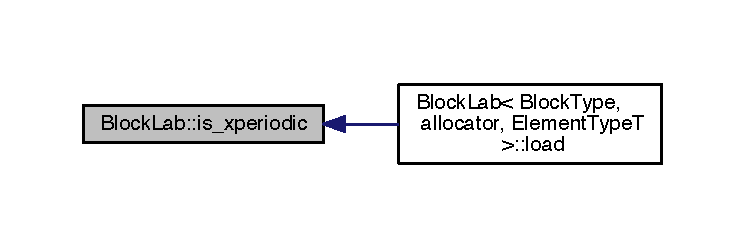
\includegraphics[width=350pt]{d7/d95/class_block_lab_aaf6e3ab940c5c3cf7463bad112527f98_icgraph}
\end{center}
\end{figure}


\hypertarget{class_block_lab_a5455e54c8e874ee9da6159ea0d1651ed}{}\index{Block\+Lab@{Block\+Lab}!is\+\_\+yperiodic@{is\+\_\+yperiodic}}
\index{is\+\_\+yperiodic@{is\+\_\+yperiodic}!Block\+Lab@{Block\+Lab}}
\subsubsection[{is\+\_\+yperiodic}]{\setlength{\rightskip}{0pt plus 5cm}template$<$typename T\+Block, template$<$ typename X $>$ class allocator = std\+::allocator, typename Element\+Type\+T = typename T\+Block\+::\+Element\+Type$>$ virtual bool {\bf Block\+Lab}$<$ T\+Block, allocator, Element\+Type\+T $>$\+::is\+\_\+yperiodic (
\begin{DoxyParamCaption}
{}
\end{DoxyParamCaption}
)\hspace{0.3cm}{\ttfamily [inline]}, {\ttfamily [virtual]}}\label{class_block_lab_a5455e54c8e874ee9da6159ea0d1651ed}


Here is the caller graph for this function\+:\nopagebreak
\begin{figure}[H]
\begin{center}
\leavevmode
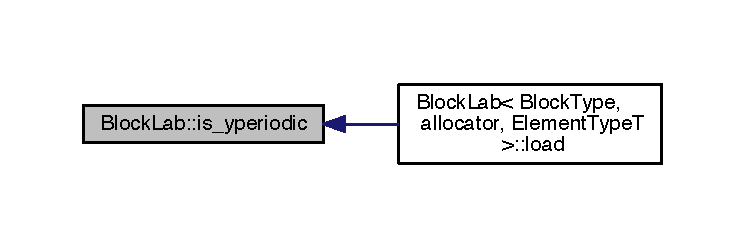
\includegraphics[width=350pt]{d7/d95/class_block_lab_a5455e54c8e874ee9da6159ea0d1651ed_icgraph}
\end{center}
\end{figure}


\hypertarget{class_block_lab_a0fd3a720fb3f2f76845ff4323e89bb91}{}\index{Block\+Lab@{Block\+Lab}!is\+\_\+zperiodic@{is\+\_\+zperiodic}}
\index{is\+\_\+zperiodic@{is\+\_\+zperiodic}!Block\+Lab@{Block\+Lab}}
\subsubsection[{is\+\_\+zperiodic}]{\setlength{\rightskip}{0pt plus 5cm}template$<$typename T\+Block, template$<$ typename X $>$ class allocator = std\+::allocator, typename Element\+Type\+T = typename T\+Block\+::\+Element\+Type$>$ virtual bool {\bf Block\+Lab}$<$ T\+Block, allocator, Element\+Type\+T $>$\+::is\+\_\+zperiodic (
\begin{DoxyParamCaption}
{}
\end{DoxyParamCaption}
)\hspace{0.3cm}{\ttfamily [inline]}, {\ttfamily [virtual]}}\label{class_block_lab_a0fd3a720fb3f2f76845ff4323e89bb91}


Here is the caller graph for this function\+:\nopagebreak
\begin{figure}[H]
\begin{center}
\leavevmode
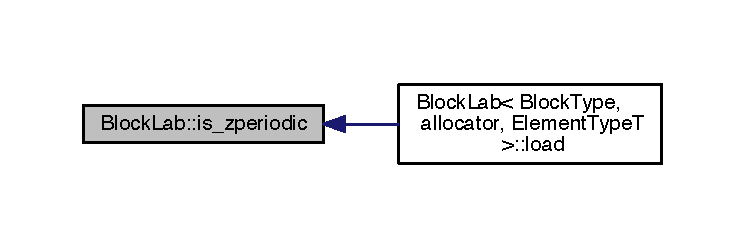
\includegraphics[width=350pt]{d7/d95/class_block_lab_a0fd3a720fb3f2f76845ff4323e89bb91_icgraph}
\end{center}
\end{figure}


\hypertarget{class_block_lab_aefd27fed8fbb1d3d60fe1457ae90f248}{}\index{Block\+Lab@{Block\+Lab}!load@{load}}
\index{load@{load}!Block\+Lab@{Block\+Lab}}
\subsubsection[{load}]{\setlength{\rightskip}{0pt plus 5cm}template$<$typename T\+Block, template$<$ typename X $>$ class allocator = std\+::allocator, typename Element\+Type\+T = typename T\+Block\+::\+Element\+Type$>$ void {\bf Block\+Lab}$<$ T\+Block, allocator, Element\+Type\+T $>$\+::load (
\begin{DoxyParamCaption}
\item[{const {\bf Block\+Info} \&}]{info, }
\item[{const {\bf Real}}]{t = {\ttfamily 0}, }
\item[{const bool}]{applybc = {\ttfamily true}}
\end{DoxyParamCaption}
)\hspace{0.3cm}{\ttfamily [inline]}}\label{class_block_lab_aefd27fed8fbb1d3d60fe1457ae90f248}
Load a block (incl. ghosts for it). This is not called internally but by the Block\+Processing-\/class. Hence a new version of \hyperlink{class_block_lab}{Block\+Lab}, can just overwrite it and through template-\/passing to Block\+Processing, the right version will be called. 
\begin{DoxyParams}{Parameters}
{\em info} & Reference to info of block to be loaded. \\
\hline
\end{DoxyParams}


Here is the caller graph for this function\+:\nopagebreak
\begin{figure}[H]
\begin{center}
\leavevmode
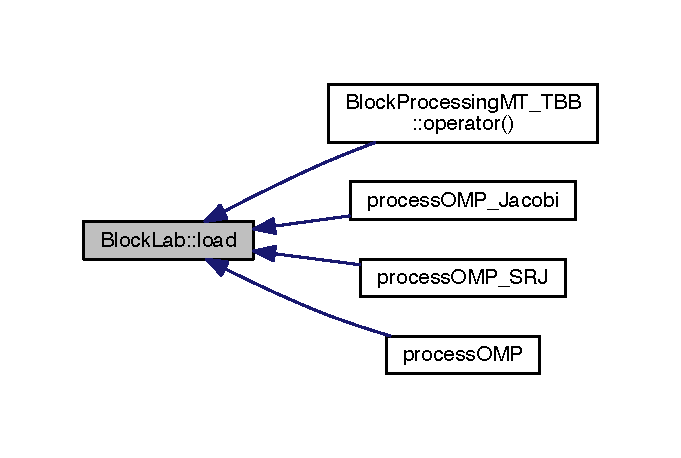
\includegraphics[width=327pt]{d7/d95/class_block_lab_aefd27fed8fbb1d3d60fe1457ae90f248_icgraph}
\end{center}
\end{figure}


\hypertarget{class_block_lab_abd79a09ab5b54cf04bfe25c125ea1edf}{}\index{Block\+Lab@{Block\+Lab}!operator()@{operator()}}
\index{operator()@{operator()}!Block\+Lab@{Block\+Lab}}
\subsubsection[{operator()}]{\setlength{\rightskip}{0pt plus 5cm}template$<$typename T\+Block, template$<$ typename X $>$ class allocator = std\+::allocator, typename Element\+Type\+T = typename T\+Block\+::\+Element\+Type$>$ {\bf Element\+Type}\& {\bf Block\+Lab}$<$ T\+Block, allocator, Element\+Type\+T $>$\+::operator() (
\begin{DoxyParamCaption}
\item[{int}]{ix, }
\item[{int}]{iy = {\ttfamily 0}, }
\item[{int}]{iz = {\ttfamily 0}}
\end{DoxyParamCaption}
)\hspace{0.3cm}{\ttfamily [inline]}}\label{class_block_lab_abd79a09ab5b54cf04bfe25c125ea1edf}
Get a single element from the block. stencil\+\_\+start and stencil\+\_\+end refer to the values passed in \hyperlink{class_block_lab_ad529f8c851da336419ad63c25ba76429}{Block\+Lab\+::prepare()}.


\begin{DoxyParams}{Parameters}
{\em ix} & Index in x-\/direction (stencil\+\_\+start\mbox{[}0\mbox{]} $<$= ix $<$ Block\+Type\+::size\+X + stencil\+\_\+end\mbox{[}0\mbox{]} -\/ 1). \\
\hline
{\em iy} & Index in y-\/direction (stencil\+\_\+start\mbox{[}1\mbox{]} $<$= iy $<$ Block\+Type\+::size\+Y + stencil\+\_\+end\mbox{[}1\mbox{]} -\/ 1). \\
\hline
{\em iz} & Index in z-\/direction (stencil\+\_\+start\mbox{[}2\mbox{]} $<$= iz $<$ Block\+Type\+::size\+Z + stencil\+\_\+end\mbox{[}2\mbox{]} -\/ 1). \\
\hline
\end{DoxyParams}
\hypertarget{class_block_lab_ad529f8c851da336419ad63c25ba76429}{}\index{Block\+Lab@{Block\+Lab}!prepare@{prepare}}
\index{prepare@{prepare}!Block\+Lab@{Block\+Lab}}
\subsubsection[{prepare}]{\setlength{\rightskip}{0pt plus 5cm}template$<$typename T\+Block, template$<$ typename X $>$ class allocator = std\+::allocator, typename Element\+Type\+T = typename T\+Block\+::\+Element\+Type$>$ void {\bf Block\+Lab}$<$ T\+Block, allocator, Element\+Type\+T $>$\+::prepare (
\begin{DoxyParamCaption}
\item[{{\bf Grid}$<$ {\bf Block\+Type}, allocator $>$ \&}]{grid, }
\item[{int}]{start\+X, }
\item[{int}]{end\+X, }
\item[{int}]{start\+Y, }
\item[{int}]{end\+Y, }
\item[{int}]{start\+Z, }
\item[{int}]{end\+Z, }
\item[{const bool}]{istensorial}
\end{DoxyParamCaption}
)\hspace{0.3cm}{\ttfamily [inline]}}\label{class_block_lab_ad529f8c851da336419ad63c25ba76429}


Here is the caller graph for this function\+:\nopagebreak
\begin{figure}[H]
\begin{center}
\leavevmode
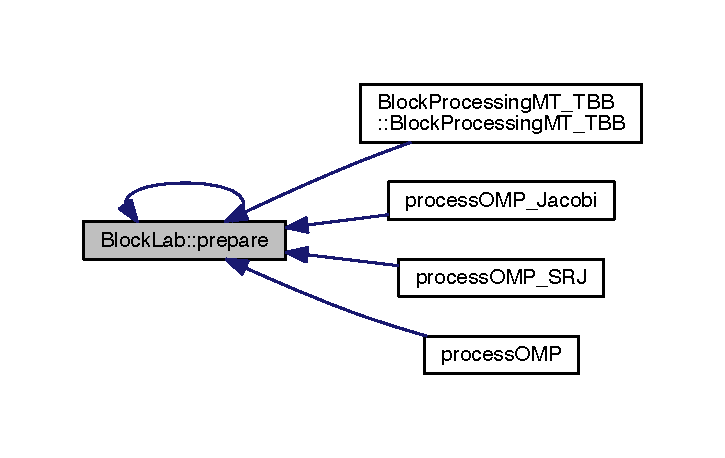
\includegraphics[width=348pt]{d7/d95/class_block_lab_ad529f8c851da336419ad63c25ba76429_icgraph}
\end{center}
\end{figure}


\hypertarget{class_block_lab_ac6236e1c94d13fa1025c8253b9855a04}{}\index{Block\+Lab@{Block\+Lab}!prepare@{prepare}}
\index{prepare@{prepare}!Block\+Lab@{Block\+Lab}}
\subsubsection[{prepare}]{\setlength{\rightskip}{0pt plus 5cm}template$<$typename T\+Block, template$<$ typename X $>$ class allocator = std\+::allocator, typename Element\+Type\+T = typename T\+Block\+::\+Element\+Type$>$ void {\bf Block\+Lab}$<$ T\+Block, allocator, Element\+Type\+T $>$\+::prepare (
\begin{DoxyParamCaption}
\item[{{\bf Grid}$<$ {\bf Block\+Type}, allocator $>$ \&}]{grid, }
\item[{const int}]{stencil\+\_\+start\mbox{[}3\mbox{]}, }
\item[{const int}]{stencil\+\_\+end\mbox{[}3\mbox{]}, }
\item[{const bool}]{istensorial}
\end{DoxyParamCaption}
)\hspace{0.3cm}{\ttfamily [inline]}}\label{class_block_lab_ac6236e1c94d13fa1025c8253b9855a04}
Prepare the extended block. 
\begin{DoxyParams}{Parameters}
{\em collection} & Collection of blocks in the grid (e.\+g. result of Grid\+::get\+Block\+Collection()). \\
\hline
{\em boundary\+Info} & Info on the boundaries of the grid (e.\+g. result of Grid\+::get\+Boundary\+Info()). \\
\hline
{\em stencil\+\_\+start} & Maximal stencil used for computations at lower boundary. Defines how many ghosts we will get in extended block. \\
\hline
{\em stencil\+\_\+end} & Maximal stencil used for computations at lower boundary. Defines how many ghosts we will get in extended block. \\
\hline
\end{DoxyParams}
\hypertarget{class_block_lab_a3e06d4124f7d69923b4ee6345c105cfc}{}\index{Block\+Lab@{Block\+Lab}!read@{read}}
\index{read@{read}!Block\+Lab@{Block\+Lab}}
\subsubsection[{read}]{\setlength{\rightskip}{0pt plus 5cm}template$<$typename T\+Block, template$<$ typename X $>$ class allocator = std\+::allocator, typename Element\+Type\+T = typename T\+Block\+::\+Element\+Type$>$ const {\bf Element\+Type}\& {\bf Block\+Lab}$<$ T\+Block, allocator, Element\+Type\+T $>$\+::read (
\begin{DoxyParamCaption}
\item[{int}]{ix, }
\item[{int}]{iy = {\ttfamily 0}, }
\item[{int}]{iz = {\ttfamily 0}}
\end{DoxyParamCaption}
) const\hspace{0.3cm}{\ttfamily [inline]}}\label{class_block_lab_a3e06d4124f7d69923b4ee6345c105cfc}
Just as Block\+Lab\+::operator() but returning a const. 

\subsection{Member Data Documentation}
\hypertarget{class_block_lab_ade306bb6935a0ead765444534c2e05db}{}\index{Block\+Lab@{Block\+Lab}!istensorial@{istensorial}}
\index{istensorial@{istensorial}!Block\+Lab@{Block\+Lab}}
\subsubsection[{istensorial}]{\setlength{\rightskip}{0pt plus 5cm}template$<$typename T\+Block, template$<$ typename X $>$ class allocator = std\+::allocator, typename Element\+Type\+T = typename T\+Block\+::\+Element\+Type$>$ bool {\bf Block\+Lab}$<$ T\+Block, allocator, Element\+Type\+T $>$\+::istensorial\hspace{0.3cm}{\ttfamily [protected]}}\label{class_block_lab_ade306bb6935a0ead765444534c2e05db}
\hypertarget{class_block_lab_aa6a4c4e00a9bb5ca5780d820b146485b}{}\index{Block\+Lab@{Block\+Lab}!m\+\_\+cache\+Block@{m\+\_\+cache\+Block}}
\index{m\+\_\+cache\+Block@{m\+\_\+cache\+Block}!Block\+Lab@{Block\+Lab}}
\subsubsection[{m\+\_\+cache\+Block}]{\setlength{\rightskip}{0pt plus 5cm}template$<$typename T\+Block, template$<$ typename X $>$ class allocator = std\+::allocator, typename Element\+Type\+T = typename T\+Block\+::\+Element\+Type$>$ {\bf Matrix3\+D}$<${\bf Element\+Type}, true, allocator$>$$\ast$ {\bf Block\+Lab}$<$ T\+Block, allocator, Element\+Type\+T $>$\+::m\+\_\+cache\+Block\hspace{0.3cm}{\ttfamily [protected]}}\label{class_block_lab_aa6a4c4e00a9bb5ca5780d820b146485b}
\hypertarget{class_block_lab_acccfe85f166f20526118fce09b28fb04}{}\index{Block\+Lab@{Block\+Lab}!m\+\_\+ref\+Grid@{m\+\_\+ref\+Grid}}
\index{m\+\_\+ref\+Grid@{m\+\_\+ref\+Grid}!Block\+Lab@{Block\+Lab}}
\subsubsection[{m\+\_\+ref\+Grid}]{\setlength{\rightskip}{0pt plus 5cm}template$<$typename T\+Block, template$<$ typename X $>$ class allocator = std\+::allocator, typename Element\+Type\+T = typename T\+Block\+::\+Element\+Type$>$ const {\bf Grid}$<${\bf Block\+Type}, allocator$>$$\ast$ {\bf Block\+Lab}$<$ T\+Block, allocator, Element\+Type\+T $>$\+::m\+\_\+ref\+Grid\hspace{0.3cm}{\ttfamily [protected]}}\label{class_block_lab_acccfe85f166f20526118fce09b28fb04}
\hypertarget{class_block_lab_a0e11603d73ab4923e1d9033edccdb572}{}\index{Block\+Lab@{Block\+Lab}!m\+\_\+state@{m\+\_\+state}}
\index{m\+\_\+state@{m\+\_\+state}!Block\+Lab@{Block\+Lab}}
\subsubsection[{m\+\_\+state}]{\setlength{\rightskip}{0pt plus 5cm}template$<$typename T\+Block, template$<$ typename X $>$ class allocator = std\+::allocator, typename Element\+Type\+T = typename T\+Block\+::\+Element\+Type$>$ {\bf e\+Block\+Lab\+\_\+\+State} {\bf Block\+Lab}$<$ T\+Block, allocator, Element\+Type\+T $>$\+::m\+\_\+state\hspace{0.3cm}{\ttfamily [protected]}}\label{class_block_lab_a0e11603d73ab4923e1d9033edccdb572}
\hypertarget{class_block_lab_a46fee08b49b11be489c71f726e258cc9}{}\index{Block\+Lab@{Block\+Lab}!m\+\_\+stencil\+End@{m\+\_\+stencil\+End}}
\index{m\+\_\+stencil\+End@{m\+\_\+stencil\+End}!Block\+Lab@{Block\+Lab}}
\subsubsection[{m\+\_\+stencil\+End}]{\setlength{\rightskip}{0pt plus 5cm}template$<$typename T\+Block, template$<$ typename X $>$ class allocator = std\+::allocator, typename Element\+Type\+T = typename T\+Block\+::\+Element\+Type$>$ int {\bf Block\+Lab}$<$ T\+Block, allocator, Element\+Type\+T $>$\+::m\+\_\+stencil\+End\mbox{[}3\mbox{]}\hspace{0.3cm}{\ttfamily [protected]}}\label{class_block_lab_a46fee08b49b11be489c71f726e258cc9}
\hypertarget{class_block_lab_a8ac6690f98ba84346a74b5b95c3afb2b}{}\index{Block\+Lab@{Block\+Lab}!m\+\_\+stencil\+Start@{m\+\_\+stencil\+Start}}
\index{m\+\_\+stencil\+Start@{m\+\_\+stencil\+Start}!Block\+Lab@{Block\+Lab}}
\subsubsection[{m\+\_\+stencil\+Start}]{\setlength{\rightskip}{0pt plus 5cm}template$<$typename T\+Block, template$<$ typename X $>$ class allocator = std\+::allocator, typename Element\+Type\+T = typename T\+Block\+::\+Element\+Type$>$ int {\bf Block\+Lab}$<$ T\+Block, allocator, Element\+Type\+T $>$\+::m\+\_\+stencil\+Start\mbox{[}3\mbox{]}\hspace{0.3cm}{\ttfamily [protected]}}\label{class_block_lab_a8ac6690f98ba84346a74b5b95c3afb2b}
\hypertarget{class_block_lab_abcd7367c6f45124d3202c8da5043ac93}{}\index{Block\+Lab@{Block\+Lab}!N\+X@{N\+X}}
\index{N\+X@{N\+X}!Block\+Lab@{Block\+Lab}}
\subsubsection[{N\+X}]{\setlength{\rightskip}{0pt plus 5cm}template$<$typename T\+Block, template$<$ typename X $>$ class allocator = std\+::allocator, typename Element\+Type\+T = typename T\+Block\+::\+Element\+Type$>$ int {\bf Block\+Lab}$<$ T\+Block, allocator, Element\+Type\+T $>$\+::N\+X\hspace{0.3cm}{\ttfamily [protected]}}\label{class_block_lab_abcd7367c6f45124d3202c8da5043ac93}
\hypertarget{class_block_lab_aaa1e748664ebb6b4fc7c47cf30a445db}{}\index{Block\+Lab@{Block\+Lab}!N\+Y@{N\+Y}}
\index{N\+Y@{N\+Y}!Block\+Lab@{Block\+Lab}}
\subsubsection[{N\+Y}]{\setlength{\rightskip}{0pt plus 5cm}template$<$typename T\+Block, template$<$ typename X $>$ class allocator = std\+::allocator, typename Element\+Type\+T = typename T\+Block\+::\+Element\+Type$>$ int {\bf Block\+Lab}$<$ T\+Block, allocator, Element\+Type\+T $>$\+::N\+Y\hspace{0.3cm}{\ttfamily [protected]}}\label{class_block_lab_aaa1e748664ebb6b4fc7c47cf30a445db}
\hypertarget{class_block_lab_acdd7f4e2489d31da6a2a76099807a7c5}{}\index{Block\+Lab@{Block\+Lab}!N\+Z@{N\+Z}}
\index{N\+Z@{N\+Z}!Block\+Lab@{Block\+Lab}}
\subsubsection[{N\+Z}]{\setlength{\rightskip}{0pt plus 5cm}template$<$typename T\+Block, template$<$ typename X $>$ class allocator = std\+::allocator, typename Element\+Type\+T = typename T\+Block\+::\+Element\+Type$>$ int {\bf Block\+Lab}$<$ T\+Block, allocator, Element\+Type\+T $>$\+::N\+Z\hspace{0.3cm}{\ttfamily [protected]}}\label{class_block_lab_acdd7f4e2489d31da6a2a76099807a7c5}


The documentation for this class was generated from the following file\+:\begin{DoxyCompactItemize}
\item 
Cubism/\hyperlink{_block_lab_8h}{Block\+Lab.\+h}\end{DoxyCompactItemize}

\hypertarget{class_block_lab_bottom_wall}{}\section{Block\+Lab\+Bottom\+Wall$<$ Block\+Type, allocator $>$ Class Template Reference}
\label{class_block_lab_bottom_wall}\index{Block\+Lab\+Bottom\+Wall$<$ Block\+Type, allocator $>$@{Block\+Lab\+Bottom\+Wall$<$ Block\+Type, allocator $>$}}


{\ttfamily \#include $<$Definitions.\+h$>$}



Inheritance diagram for Block\+Lab\+Bottom\+Wall$<$ Block\+Type, allocator $>$\+:
\nopagebreak
\begin{figure}[H]
\begin{center}
\leavevmode
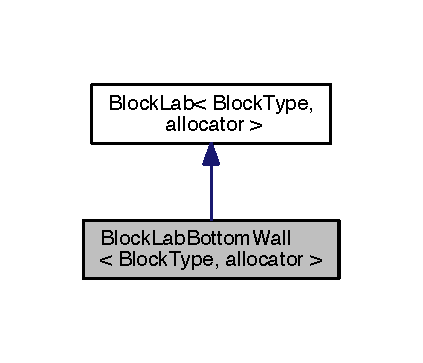
\includegraphics[width=203pt]{df/d16/class_block_lab_bottom_wall__inherit__graph}
\end{center}
\end{figure}


Collaboration diagram for Block\+Lab\+Bottom\+Wall$<$ Block\+Type, allocator $>$\+:
\nopagebreak
\begin{figure}[H]
\begin{center}
\leavevmode
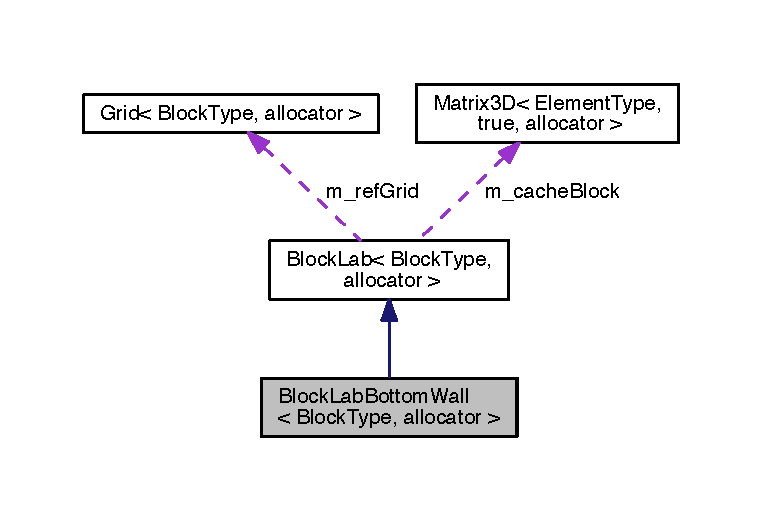
\includegraphics[width=350pt]{d7/dc5/class_block_lab_bottom_wall__coll__graph}
\end{center}
\end{figure}
\subsection*{Public Member Functions}
\begin{DoxyCompactItemize}
\item 
\hyperlink{class_block_lab_bottom_wall_a89c8bb288dd9480f0b6bed2d27d4646d}{Block\+Lab\+Bottom\+Wall} ()
\item 
void \hyperlink{class_block_lab_bottom_wall_a76208c2636c75bdfe9a452a35bcb0c38}{\+\_\+apply\+\_\+bc} (const \hyperlink{struct_block_info}{Block\+Info} \&info, const \hyperlink{_h_d_f5_dumper_8h_a445a5f0e2a34c9d97d69a3c2d1957907}{Real} t=0)
\end{DoxyCompactItemize}
\subsection*{Additional Inherited Members}


\subsection{Constructor \& Destructor Documentation}
\hypertarget{class_block_lab_bottom_wall_a89c8bb288dd9480f0b6bed2d27d4646d}{}\index{Block\+Lab\+Bottom\+Wall@{Block\+Lab\+Bottom\+Wall}!Block\+Lab\+Bottom\+Wall@{Block\+Lab\+Bottom\+Wall}}
\index{Block\+Lab\+Bottom\+Wall@{Block\+Lab\+Bottom\+Wall}!Block\+Lab\+Bottom\+Wall@{Block\+Lab\+Bottom\+Wall}}
\subsubsection[{Block\+Lab\+Bottom\+Wall}]{\setlength{\rightskip}{0pt plus 5cm}template$<$typename Block\+Type , template$<$ typename X $>$ class allocator = std\+::allocator$>$ {\bf Block\+Lab\+Bottom\+Wall}$<$ {\bf Block\+Type}, allocator $>$\+::{\bf Block\+Lab\+Bottom\+Wall} (
\begin{DoxyParamCaption}
{}
\end{DoxyParamCaption}
)\hspace{0.3cm}{\ttfamily [inline]}}\label{class_block_lab_bottom_wall_a89c8bb288dd9480f0b6bed2d27d4646d}


\subsection{Member Function Documentation}
\hypertarget{class_block_lab_bottom_wall_a76208c2636c75bdfe9a452a35bcb0c38}{}\index{Block\+Lab\+Bottom\+Wall@{Block\+Lab\+Bottom\+Wall}!\+\_\+apply\+\_\+bc@{\+\_\+apply\+\_\+bc}}
\index{\+\_\+apply\+\_\+bc@{\+\_\+apply\+\_\+bc}!Block\+Lab\+Bottom\+Wall@{Block\+Lab\+Bottom\+Wall}}
\subsubsection[{\+\_\+apply\+\_\+bc}]{\setlength{\rightskip}{0pt plus 5cm}template$<$typename Block\+Type , template$<$ typename X $>$ class allocator = std\+::allocator$>$ void {\bf Block\+Lab\+Bottom\+Wall}$<$ {\bf Block\+Type}, allocator $>$\+::\+\_\+apply\+\_\+bc (
\begin{DoxyParamCaption}
\item[{const {\bf Block\+Info} \&}]{info, }
\item[{const {\bf Real}}]{t = {\ttfamily 0}}
\end{DoxyParamCaption}
)\hspace{0.3cm}{\ttfamily [inline]}, {\ttfamily [virtual]}}\label{class_block_lab_bottom_wall_a76208c2636c75bdfe9a452a35bcb0c38}


Reimplemented from \hyperlink{class_block_lab_a669ac139b57be4967e5f43bc649a8520}{Block\+Lab$<$ Block\+Type, allocator $>$}.



The documentation for this class was generated from the following file\+:\begin{DoxyCompactItemize}
\item 
/\+Users/cconti/\+Desktop/\+Mounts/\+Brutus\+Home/\+Cubism\+U\+P\+\_\+2\+D/source/\hyperlink{_definitions_8h}{Definitions.\+h}\end{DoxyCompactItemize}

\hypertarget{class_block_lab_box}{}\section{Block\+Lab\+Box$<$ Block\+Type, allocator $>$ Class Template Reference}
\label{class_block_lab_box}\index{Block\+Lab\+Box$<$ Block\+Type, allocator $>$@{Block\+Lab\+Box$<$ Block\+Type, allocator $>$}}


{\ttfamily \#include $<$Definitions.\+h$>$}



Inheritance diagram for Block\+Lab\+Box$<$ Block\+Type, allocator $>$\+:\nopagebreak
\begin{figure}[H]
\begin{center}
\leavevmode
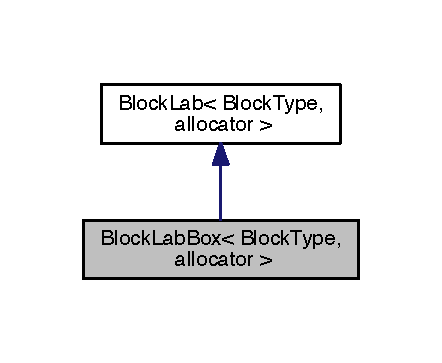
\includegraphics[width=212pt]{d8/d35/class_block_lab_box__inherit__graph}
\end{center}
\end{figure}


Collaboration diagram for Block\+Lab\+Box$<$ Block\+Type, allocator $>$\+:\nopagebreak
\begin{figure}[H]
\begin{center}
\leavevmode
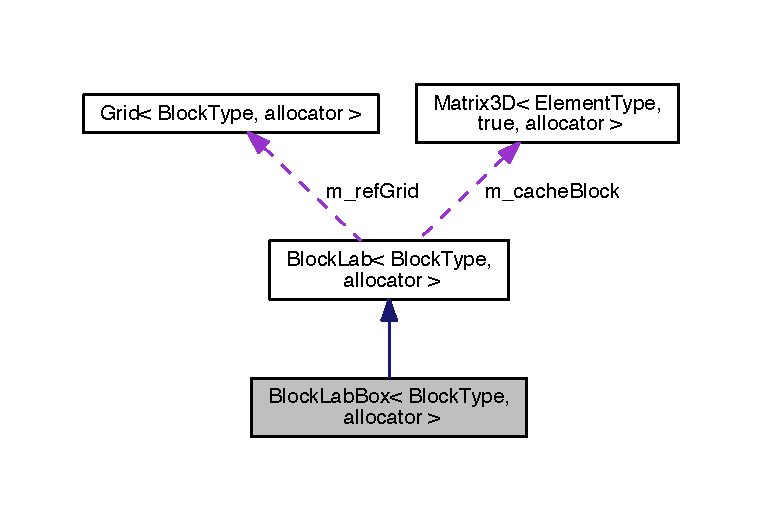
\includegraphics[width=350pt]{d0/d61/class_block_lab_box__coll__graph}
\end{center}
\end{figure}
\subsection*{Public Member Functions}
\begin{DoxyCompactItemize}
\item 
\hyperlink{class_block_lab_box_a819b297579990253484d7fed5dc878db}{Block\+Lab\+Box} ()
\item 
void \hyperlink{class_block_lab_box_adfd9b3d46062be59f03d0c1df79db81d}{\+\_\+apply\+\_\+bc} (const \hyperlink{struct_block_info}{Block\+Info} \&info, const \hyperlink{_h_d_f5_dumper_8h_a445a5f0e2a34c9d97d69a3c2d1957907}{Real} t=0)
\end{DoxyCompactItemize}
\subsection*{Additional Inherited Members}


\subsection{Constructor \& Destructor Documentation}
\hypertarget{class_block_lab_box_a819b297579990253484d7fed5dc878db}{}\index{Block\+Lab\+Box@{Block\+Lab\+Box}!Block\+Lab\+Box@{Block\+Lab\+Box}}
\index{Block\+Lab\+Box@{Block\+Lab\+Box}!Block\+Lab\+Box@{Block\+Lab\+Box}}
\subsubsection[{Block\+Lab\+Box}]{\setlength{\rightskip}{0pt plus 5cm}template$<$typename Block\+Type , template$<$ typename X $>$ class allocator = std\+::allocator$>$ {\bf Block\+Lab\+Box}$<$ {\bf Block\+Type}, allocator $>$\+::{\bf Block\+Lab\+Box} (
\begin{DoxyParamCaption}
{}
\end{DoxyParamCaption}
)\hspace{0.3cm}{\ttfamily [inline]}}\label{class_block_lab_box_a819b297579990253484d7fed5dc878db}


\subsection{Member Function Documentation}
\hypertarget{class_block_lab_box_adfd9b3d46062be59f03d0c1df79db81d}{}\index{Block\+Lab\+Box@{Block\+Lab\+Box}!\+\_\+apply\+\_\+bc@{\+\_\+apply\+\_\+bc}}
\index{\+\_\+apply\+\_\+bc@{\+\_\+apply\+\_\+bc}!Block\+Lab\+Box@{Block\+Lab\+Box}}
\subsubsection[{\+\_\+apply\+\_\+bc}]{\setlength{\rightskip}{0pt plus 5cm}template$<$typename Block\+Type , template$<$ typename X $>$ class allocator = std\+::allocator$>$ void {\bf Block\+Lab\+Box}$<$ {\bf Block\+Type}, allocator $>$\+::\+\_\+apply\+\_\+bc (
\begin{DoxyParamCaption}
\item[{const {\bf Block\+Info} \&}]{info, }
\item[{const {\bf Real}}]{t = {\ttfamily 0}}
\end{DoxyParamCaption}
)\hspace{0.3cm}{\ttfamily [inline]}, {\ttfamily [virtual]}}\label{class_block_lab_box_adfd9b3d46062be59f03d0c1df79db81d}


Reimplemented from \hyperlink{class_block_lab_a669ac139b57be4967e5f43bc649a8520}{Block\+Lab$<$ Block\+Type, allocator $>$}.



The documentation for this class was generated from the following file\+:\begin{DoxyCompactItemize}
\item 
/\+Users/cconti/\+Desktop/\+Mounts/\+Brutus\+Home/\+Cubism\+U\+P\+\_\+2\+D/source/\hyperlink{_definitions_8h}{Definitions.\+h}\end{DoxyCompactItemize}

\hypertarget{class_block_lab_dirichlet}{}\section{Block\+Lab\+Dirichlet$<$ Block\+Type, allocator $>$ Class Template Reference}
\label{class_block_lab_dirichlet}\index{Block\+Lab\+Dirichlet$<$ Block\+Type, allocator $>$@{Block\+Lab\+Dirichlet$<$ Block\+Type, allocator $>$}}


{\ttfamily \#include $<$Definitions.\+h$>$}



Inheritance diagram for Block\+Lab\+Dirichlet$<$ Block\+Type, allocator $>$\+:\nopagebreak
\begin{figure}[H]
\begin{center}
\leavevmode
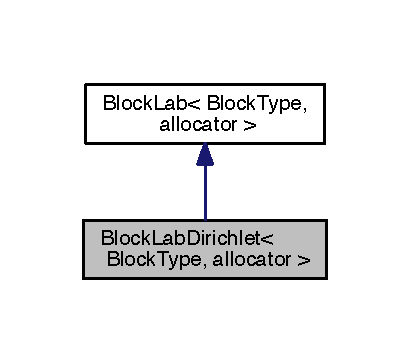
\includegraphics[width=197pt]{d6/d91/class_block_lab_dirichlet__inherit__graph}
\end{center}
\end{figure}


Collaboration diagram for Block\+Lab\+Dirichlet$<$ Block\+Type, allocator $>$\+:\nopagebreak
\begin{figure}[H]
\begin{center}
\leavevmode
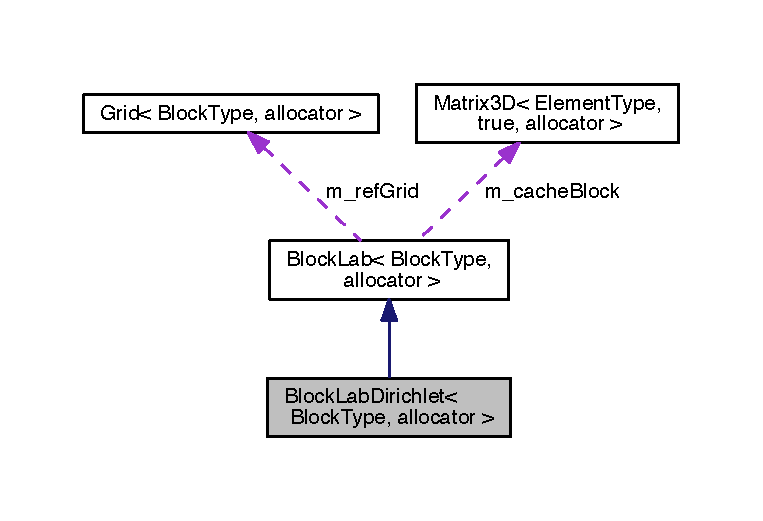
\includegraphics[width=350pt]{dc/dfc/class_block_lab_dirichlet__coll__graph}
\end{center}
\end{figure}
\subsection*{Public Member Functions}
\begin{DoxyCompactItemize}
\item 
\hyperlink{class_block_lab_dirichlet_aee522a1b0a5e8047dea4558b34df6141}{Block\+Lab\+Dirichlet} ()
\item 
void \hyperlink{class_block_lab_dirichlet_ae05580142a8ddb65c42fd92063355609}{\+\_\+apply\+\_\+bc} (const \hyperlink{struct_block_info}{Block\+Info} \&info, const \hyperlink{_h_d_f5_dumper_8h_a445a5f0e2a34c9d97d69a3c2d1957907}{Real} t=0)
\end{DoxyCompactItemize}
\subsection*{Additional Inherited Members}


\subsection{Constructor \& Destructor Documentation}
\hypertarget{class_block_lab_dirichlet_aee522a1b0a5e8047dea4558b34df6141}{}\index{Block\+Lab\+Dirichlet@{Block\+Lab\+Dirichlet}!Block\+Lab\+Dirichlet@{Block\+Lab\+Dirichlet}}
\index{Block\+Lab\+Dirichlet@{Block\+Lab\+Dirichlet}!Block\+Lab\+Dirichlet@{Block\+Lab\+Dirichlet}}
\subsubsection[{Block\+Lab\+Dirichlet}]{\setlength{\rightskip}{0pt plus 5cm}template$<$typename Block\+Type , template$<$ typename X $>$ class allocator = std\+::allocator$>$ {\bf Block\+Lab\+Dirichlet}$<$ {\bf Block\+Type}, allocator $>$\+::{\bf Block\+Lab\+Dirichlet} (
\begin{DoxyParamCaption}
{}
\end{DoxyParamCaption}
)\hspace{0.3cm}{\ttfamily [inline]}}\label{class_block_lab_dirichlet_aee522a1b0a5e8047dea4558b34df6141}


\subsection{Member Function Documentation}
\hypertarget{class_block_lab_dirichlet_ae05580142a8ddb65c42fd92063355609}{}\index{Block\+Lab\+Dirichlet@{Block\+Lab\+Dirichlet}!\+\_\+apply\+\_\+bc@{\+\_\+apply\+\_\+bc}}
\index{\+\_\+apply\+\_\+bc@{\+\_\+apply\+\_\+bc}!Block\+Lab\+Dirichlet@{Block\+Lab\+Dirichlet}}
\subsubsection[{\+\_\+apply\+\_\+bc}]{\setlength{\rightskip}{0pt plus 5cm}template$<$typename Block\+Type , template$<$ typename X $>$ class allocator = std\+::allocator$>$ void {\bf Block\+Lab\+Dirichlet}$<$ {\bf Block\+Type}, allocator $>$\+::\+\_\+apply\+\_\+bc (
\begin{DoxyParamCaption}
\item[{const {\bf Block\+Info} \&}]{info, }
\item[{const {\bf Real}}]{t = {\ttfamily 0}}
\end{DoxyParamCaption}
)\hspace{0.3cm}{\ttfamily [inline]}, {\ttfamily [virtual]}}\label{class_block_lab_dirichlet_ae05580142a8ddb65c42fd92063355609}


Reimplemented from \hyperlink{class_block_lab_a669ac139b57be4967e5f43bc649a8520}{Block\+Lab$<$ Block\+Type, allocator $>$}.



The documentation for this class was generated from the following file\+:\begin{DoxyCompactItemize}
\item 
source/\hyperlink{_definitions_8h}{Definitions.\+h}\end{DoxyCompactItemize}

\hypertarget{class_block_lab_m_p_i}{}\section{Block\+Lab\+M\+P\+I$<$ My\+Block\+Lab $>$ Class Template Reference}
\label{class_block_lab_m_p_i}\index{Block\+Lab\+M\+P\+I$<$ My\+Block\+Lab $>$@{Block\+Lab\+M\+P\+I$<$ My\+Block\+Lab $>$}}


{\ttfamily \#include $<$Block\+Lab\+M\+P\+I.\+h$>$}



Inheritance diagram for Block\+Lab\+M\+P\+I$<$ My\+Block\+Lab $>$\+:
% FIG 0


Collaboration diagram for Block\+Lab\+M\+P\+I$<$ My\+Block\+Lab $>$\+:
% FIG 1
\subsection*{Public Member Functions}
\begin{DoxyCompactItemize}
\item 
{\footnotesize template$<$typename T\+Grid $>$ }\\void \hyperlink{class_block_lab_m_p_i_a49e9b846d16c1c3f177b6ff067bc791c}{prepare} (\hyperlink{class_grid_m_p_i}{Grid\+M\+P\+I}$<$ T\+Grid $>$ \&grid, const \hyperlink{class_synchronizer_m_p_i}{Synchronizer\+M\+P\+I} \&\hyperlink{class_synchronizer_m_p_i}{Synchronizer\+M\+P\+I})
\item 
void \hyperlink{class_block_lab_m_p_i_a9695a460545974a0aa473039c3876765}{load} (const \hyperlink{struct_block_info}{Block\+Info} \&info, const \hyperlink{_h_d_f5_dumper_8h_a445a5f0e2a34c9d97d69a3c2d1957907}{Real} t=0, const bool applybc=true)
\end{DoxyCompactItemize}
\subsection*{Protected Attributes}
\begin{DoxyCompactItemize}
\item 
int \hyperlink{class_block_lab_m_p_i_a346371e08c48393a09a60188aa210828}{mypeindex} \mbox{[}3\mbox{]}
\item 
int \hyperlink{class_block_lab_m_p_i_a3c58102452df2ae20110af79d504693e}{pesize} \mbox{[}3\mbox{]}
\item 
int \hyperlink{class_block_lab_m_p_i_a11a592341f9c28f07809f0d950512fe5}{mybpd} \mbox{[}3\mbox{]}
\item 
int \hyperlink{class_block_lab_m_p_i_a41646b94f197315e4c39c5155ee939eb}{g\+Last\+X}
\item 
int \hyperlink{class_block_lab_m_p_i_afc336a0d08b78a9196eb24701816d6c8}{g\+Last\+Y}
\item 
int \hyperlink{class_block_lab_m_p_i_a8b9247a3ec2caad18896f597b98b7103}{g\+Last\+Z}
\end{DoxyCompactItemize}


\subsection{Member Function Documentation}
\hypertarget{class_block_lab_m_p_i_a9695a460545974a0aa473039c3876765}{}\index{Block\+Lab\+M\+P\+I@{Block\+Lab\+M\+P\+I}!load@{load}}
\index{load@{load}!Block\+Lab\+M\+P\+I@{Block\+Lab\+M\+P\+I}}
\subsubsection[{load}]{\setlength{\rightskip}{0pt plus 5cm}template$<$typename My\+Block\+Lab $>$ void {\bf Block\+Lab\+M\+P\+I}$<$ My\+Block\+Lab $>$\+::load (
\begin{DoxyParamCaption}
\item[{const {\bf Block\+Info} \&}]{info, }
\item[{const {\bf Real}}]{t = {\ttfamily 0}, }
\item[{const bool}]{applybc = {\ttfamily true}}
\end{DoxyParamCaption}
)\hspace{0.3cm}{\ttfamily [inline]}}\label{class_block_lab_m_p_i_a9695a460545974a0aa473039c3876765}


Here is the call graph for this function\+:
% FIG 2


\hypertarget{class_block_lab_m_p_i_a49e9b846d16c1c3f177b6ff067bc791c}{}\index{Block\+Lab\+M\+P\+I@{Block\+Lab\+M\+P\+I}!prepare@{prepare}}
\index{prepare@{prepare}!Block\+Lab\+M\+P\+I@{Block\+Lab\+M\+P\+I}}
\subsubsection[{prepare}]{\setlength{\rightskip}{0pt plus 5cm}template$<$typename My\+Block\+Lab $>$ template$<$typename T\+Grid $>$ void {\bf Block\+Lab\+M\+P\+I}$<$ My\+Block\+Lab $>$\+::prepare (
\begin{DoxyParamCaption}
\item[{{\bf Grid\+M\+P\+I}$<$ T\+Grid $>$ \&}]{grid, }
\item[{const {\bf Synchronizer\+M\+P\+I} \&}]{Synchronizer\+M\+P\+I}
\end{DoxyParamCaption}
)\hspace{0.3cm}{\ttfamily [inline]}}\label{class_block_lab_m_p_i_a49e9b846d16c1c3f177b6ff067bc791c}


Here is the call graph for this function\+:
% FIG 3




\subsection{Member Data Documentation}
\hypertarget{class_block_lab_m_p_i_a41646b94f197315e4c39c5155ee939eb}{}\index{Block\+Lab\+M\+P\+I@{Block\+Lab\+M\+P\+I}!g\+Last\+X@{g\+Last\+X}}
\index{g\+Last\+X@{g\+Last\+X}!Block\+Lab\+M\+P\+I@{Block\+Lab\+M\+P\+I}}
\subsubsection[{g\+Last\+X}]{\setlength{\rightskip}{0pt plus 5cm}template$<$typename My\+Block\+Lab $>$ int {\bf Block\+Lab\+M\+P\+I}$<$ My\+Block\+Lab $>$\+::g\+Last\+X\hspace{0.3cm}{\ttfamily [protected]}}\label{class_block_lab_m_p_i_a41646b94f197315e4c39c5155ee939eb}
\hypertarget{class_block_lab_m_p_i_afc336a0d08b78a9196eb24701816d6c8}{}\index{Block\+Lab\+M\+P\+I@{Block\+Lab\+M\+P\+I}!g\+Last\+Y@{g\+Last\+Y}}
\index{g\+Last\+Y@{g\+Last\+Y}!Block\+Lab\+M\+P\+I@{Block\+Lab\+M\+P\+I}}
\subsubsection[{g\+Last\+Y}]{\setlength{\rightskip}{0pt plus 5cm}template$<$typename My\+Block\+Lab $>$ int {\bf Block\+Lab\+M\+P\+I}$<$ My\+Block\+Lab $>$\+::g\+Last\+Y\hspace{0.3cm}{\ttfamily [protected]}}\label{class_block_lab_m_p_i_afc336a0d08b78a9196eb24701816d6c8}
\hypertarget{class_block_lab_m_p_i_a8b9247a3ec2caad18896f597b98b7103}{}\index{Block\+Lab\+M\+P\+I@{Block\+Lab\+M\+P\+I}!g\+Last\+Z@{g\+Last\+Z}}
\index{g\+Last\+Z@{g\+Last\+Z}!Block\+Lab\+M\+P\+I@{Block\+Lab\+M\+P\+I}}
\subsubsection[{g\+Last\+Z}]{\setlength{\rightskip}{0pt plus 5cm}template$<$typename My\+Block\+Lab $>$ int {\bf Block\+Lab\+M\+P\+I}$<$ My\+Block\+Lab $>$\+::g\+Last\+Z\hspace{0.3cm}{\ttfamily [protected]}}\label{class_block_lab_m_p_i_a8b9247a3ec2caad18896f597b98b7103}
\hypertarget{class_block_lab_m_p_i_a11a592341f9c28f07809f0d950512fe5}{}\index{Block\+Lab\+M\+P\+I@{Block\+Lab\+M\+P\+I}!mybpd@{mybpd}}
\index{mybpd@{mybpd}!Block\+Lab\+M\+P\+I@{Block\+Lab\+M\+P\+I}}
\subsubsection[{mybpd}]{\setlength{\rightskip}{0pt plus 5cm}template$<$typename My\+Block\+Lab $>$ int {\bf Block\+Lab\+M\+P\+I}$<$ My\+Block\+Lab $>$\+::mybpd\mbox{[}3\mbox{]}\hspace{0.3cm}{\ttfamily [protected]}}\label{class_block_lab_m_p_i_a11a592341f9c28f07809f0d950512fe5}
\hypertarget{class_block_lab_m_p_i_a346371e08c48393a09a60188aa210828}{}\index{Block\+Lab\+M\+P\+I@{Block\+Lab\+M\+P\+I}!mypeindex@{mypeindex}}
\index{mypeindex@{mypeindex}!Block\+Lab\+M\+P\+I@{Block\+Lab\+M\+P\+I}}
\subsubsection[{mypeindex}]{\setlength{\rightskip}{0pt plus 5cm}template$<$typename My\+Block\+Lab $>$ int {\bf Block\+Lab\+M\+P\+I}$<$ My\+Block\+Lab $>$\+::mypeindex\mbox{[}3\mbox{]}\hspace{0.3cm}{\ttfamily [protected]}}\label{class_block_lab_m_p_i_a346371e08c48393a09a60188aa210828}
\hypertarget{class_block_lab_m_p_i_a3c58102452df2ae20110af79d504693e}{}\index{Block\+Lab\+M\+P\+I@{Block\+Lab\+M\+P\+I}!pesize@{pesize}}
\index{pesize@{pesize}!Block\+Lab\+M\+P\+I@{Block\+Lab\+M\+P\+I}}
\subsubsection[{pesize}]{\setlength{\rightskip}{0pt plus 5cm}template$<$typename My\+Block\+Lab $>$ int {\bf Block\+Lab\+M\+P\+I}$<$ My\+Block\+Lab $>$\+::pesize\mbox{[}3\mbox{]}\hspace{0.3cm}{\ttfamily [protected]}}\label{class_block_lab_m_p_i_a3c58102452df2ae20110af79d504693e}


The documentation for this class was generated from the following file\+:\begin{DoxyCompactItemize}
\item 
/\+Users/cconti/\+Desktop/\+Mounts/\+Brutus\+Home/\+Seed/\+Cubism\+U\+P\+\_\+2\+D/\+Cubism/\hyperlink{_block_lab_m_p_i_8h}{Block\+Lab\+M\+P\+I.\+h}\end{DoxyCompactItemize}

\hypertarget{class_block_lab_neumann}{}\section{Block\+Lab\+Neumann$<$ Block\+Type, allocator $>$ Class Template Reference}
\label{class_block_lab_neumann}\index{Block\+Lab\+Neumann$<$ Block\+Type, allocator $>$@{Block\+Lab\+Neumann$<$ Block\+Type, allocator $>$}}


{\ttfamily \#include $<$Definitions.\+h$>$}



Inheritance diagram for Block\+Lab\+Neumann$<$ Block\+Type, allocator $>$\+:
% FIG 0


Collaboration diagram for Block\+Lab\+Neumann$<$ Block\+Type, allocator $>$\+:
% FIG 1
\subsection*{Public Member Functions}
\begin{DoxyCompactItemize}
\item 
\hyperlink{class_block_lab_neumann_ab365064c3cc0d442c730d90cd8c5bd0b}{Block\+Lab\+Neumann} ()
\item 
void \hyperlink{class_block_lab_neumann_a65cd80126a426fa2aa098910fd189793}{\+\_\+apply\+\_\+bc} (const \hyperlink{struct_block_info}{Block\+Info} \&info, const \hyperlink{_h_d_f5_dumper_8h_a445a5f0e2a34c9d97d69a3c2d1957907}{Real} t=0)
\end{DoxyCompactItemize}
\subsection*{Additional Inherited Members}


\subsection{Constructor \& Destructor Documentation}
\hypertarget{class_block_lab_neumann_ab365064c3cc0d442c730d90cd8c5bd0b}{}\index{Block\+Lab\+Neumann@{Block\+Lab\+Neumann}!Block\+Lab\+Neumann@{Block\+Lab\+Neumann}}
\index{Block\+Lab\+Neumann@{Block\+Lab\+Neumann}!Block\+Lab\+Neumann@{Block\+Lab\+Neumann}}
\subsubsection[{Block\+Lab\+Neumann}]{\setlength{\rightskip}{0pt plus 5cm}template$<$typename Block\+Type , template$<$ typename X $>$ class allocator = std\+::allocator$>$ {\bf Block\+Lab\+Neumann}$<$ {\bf Block\+Type}, allocator $>$\+::{\bf Block\+Lab\+Neumann} (
\begin{DoxyParamCaption}
{}
\end{DoxyParamCaption}
)\hspace{0.3cm}{\ttfamily [inline]}}\label{class_block_lab_neumann_ab365064c3cc0d442c730d90cd8c5bd0b}


\subsection{Member Function Documentation}
\hypertarget{class_block_lab_neumann_a65cd80126a426fa2aa098910fd189793}{}\index{Block\+Lab\+Neumann@{Block\+Lab\+Neumann}!\+\_\+apply\+\_\+bc@{\+\_\+apply\+\_\+bc}}
\index{\+\_\+apply\+\_\+bc@{\+\_\+apply\+\_\+bc}!Block\+Lab\+Neumann@{Block\+Lab\+Neumann}}
\subsubsection[{\+\_\+apply\+\_\+bc}]{\setlength{\rightskip}{0pt plus 5cm}template$<$typename Block\+Type , template$<$ typename X $>$ class allocator = std\+::allocator$>$ void {\bf Block\+Lab\+Neumann}$<$ {\bf Block\+Type}, allocator $>$\+::\+\_\+apply\+\_\+bc (
\begin{DoxyParamCaption}
\item[{const {\bf Block\+Info} \&}]{info, }
\item[{const {\bf Real}}]{t = {\ttfamily 0}}
\end{DoxyParamCaption}
)\hspace{0.3cm}{\ttfamily [inline]}, {\ttfamily [virtual]}}\label{class_block_lab_neumann_a65cd80126a426fa2aa098910fd189793}


Reimplemented from \hyperlink{class_block_lab_a669ac139b57be4967e5f43bc649a8520}{Block\+Lab$<$ Block\+Type, allocator $>$}.



The documentation for this class was generated from the following file\+:\begin{DoxyCompactItemize}
\item 
/\+Users/cconti/\+Desktop/\+Mounts/\+Brutus\+Home/\+Seed/\+Cubism\+U\+P\+\_\+2\+D/source/\hyperlink{_definitions_8h}{Definitions.\+h}\end{DoxyCompactItemize}

\hypertarget{class_block_lab_pipe}{}\section{Block\+Lab\+Pipe$<$ Block\+Type, allocator $>$ Class Template Reference}
\label{class_block_lab_pipe}\index{Block\+Lab\+Pipe$<$ Block\+Type, allocator $>$@{Block\+Lab\+Pipe$<$ Block\+Type, allocator $>$}}


{\ttfamily \#include $<$Definitions.\+h$>$}



Inheritance diagram for Block\+Lab\+Pipe$<$ Block\+Type, allocator $>$\+:\nopagebreak
\begin{figure}[H]
\begin{center}
\leavevmode
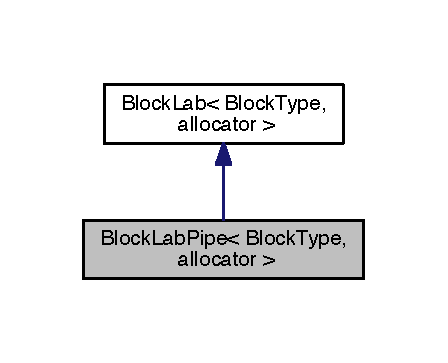
\includegraphics[width=215pt]{d1/dfa/class_block_lab_pipe__inherit__graph}
\end{center}
\end{figure}


Collaboration diagram for Block\+Lab\+Pipe$<$ Block\+Type, allocator $>$\+:\nopagebreak
\begin{figure}[H]
\begin{center}
\leavevmode
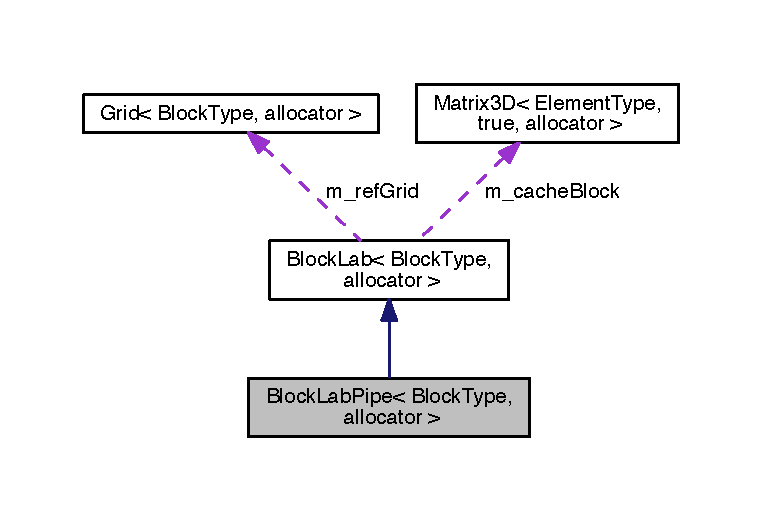
\includegraphics[width=350pt]{da/d2a/class_block_lab_pipe__coll__graph}
\end{center}
\end{figure}
\subsection*{Public Member Functions}
\begin{DoxyCompactItemize}
\item 
\hyperlink{class_block_lab_pipe_a915d4349dcab5bf24de0778e0cd99e14}{Block\+Lab\+Pipe} ()
\item 
void \hyperlink{class_block_lab_pipe_a9aa9d7d5604194dd0af8255a7533c288}{\+\_\+apply\+\_\+bc} (const \hyperlink{struct_block_info}{Block\+Info} \&info, const \hyperlink{_h_d_f5_dumper_8h_a445a5f0e2a34c9d97d69a3c2d1957907}{Real} t=0)
\end{DoxyCompactItemize}
\subsection*{Additional Inherited Members}


\subsection{Constructor \& Destructor Documentation}
\hypertarget{class_block_lab_pipe_a915d4349dcab5bf24de0778e0cd99e14}{}\index{Block\+Lab\+Pipe@{Block\+Lab\+Pipe}!Block\+Lab\+Pipe@{Block\+Lab\+Pipe}}
\index{Block\+Lab\+Pipe@{Block\+Lab\+Pipe}!Block\+Lab\+Pipe@{Block\+Lab\+Pipe}}
\subsubsection[{Block\+Lab\+Pipe}]{\setlength{\rightskip}{0pt plus 5cm}template$<$typename Block\+Type , template$<$ typename X $>$ class allocator = std\+::allocator$>$ {\bf Block\+Lab\+Pipe}$<$ {\bf Block\+Type}, allocator $>$\+::{\bf Block\+Lab\+Pipe} (
\begin{DoxyParamCaption}
{}
\end{DoxyParamCaption}
)\hspace{0.3cm}{\ttfamily [inline]}}\label{class_block_lab_pipe_a915d4349dcab5bf24de0778e0cd99e14}


\subsection{Member Function Documentation}
\hypertarget{class_block_lab_pipe_a9aa9d7d5604194dd0af8255a7533c288}{}\index{Block\+Lab\+Pipe@{Block\+Lab\+Pipe}!\+\_\+apply\+\_\+bc@{\+\_\+apply\+\_\+bc}}
\index{\+\_\+apply\+\_\+bc@{\+\_\+apply\+\_\+bc}!Block\+Lab\+Pipe@{Block\+Lab\+Pipe}}
\subsubsection[{\+\_\+apply\+\_\+bc}]{\setlength{\rightskip}{0pt plus 5cm}template$<$typename Block\+Type , template$<$ typename X $>$ class allocator = std\+::allocator$>$ void {\bf Block\+Lab\+Pipe}$<$ {\bf Block\+Type}, allocator $>$\+::\+\_\+apply\+\_\+bc (
\begin{DoxyParamCaption}
\item[{const {\bf Block\+Info} \&}]{info, }
\item[{const {\bf Real}}]{t = {\ttfamily 0}}
\end{DoxyParamCaption}
)\hspace{0.3cm}{\ttfamily [inline]}, {\ttfamily [virtual]}}\label{class_block_lab_pipe_a9aa9d7d5604194dd0af8255a7533c288}


Reimplemented from \hyperlink{class_block_lab_a669ac139b57be4967e5f43bc649a8520}{Block\+Lab$<$ Block\+Type, allocator $>$}.



The documentation for this class was generated from the following file\+:\begin{DoxyCompactItemize}
\item 
/\+Users/cconti/\+Desktop/\+Mounts/\+Brutus\+Home/\+Cubism\+U\+P\+\_\+2\+D/source/\hyperlink{_definitions_8h}{Definitions.\+h}\end{DoxyCompactItemize}

\hypertarget{class_block_lab_vortex}{}\section{Block\+Lab\+Vortex$<$ Block\+Type, allocator $>$ Class Template Reference}
\label{class_block_lab_vortex}\index{Block\+Lab\+Vortex$<$ Block\+Type, allocator $>$@{Block\+Lab\+Vortex$<$ Block\+Type, allocator $>$}}


{\ttfamily \#include $<$Definitions.\+h$>$}



Inheritance diagram for Block\+Lab\+Vortex$<$ Block\+Type, allocator $>$\+:\nopagebreak
\begin{figure}[H]
\begin{center}
\leavevmode
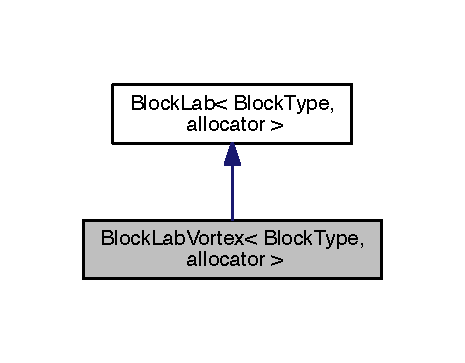
\includegraphics[width=223pt]{da/d22/class_block_lab_vortex__inherit__graph}
\end{center}
\end{figure}


Collaboration diagram for Block\+Lab\+Vortex$<$ Block\+Type, allocator $>$\+:\nopagebreak
\begin{figure}[H]
\begin{center}
\leavevmode
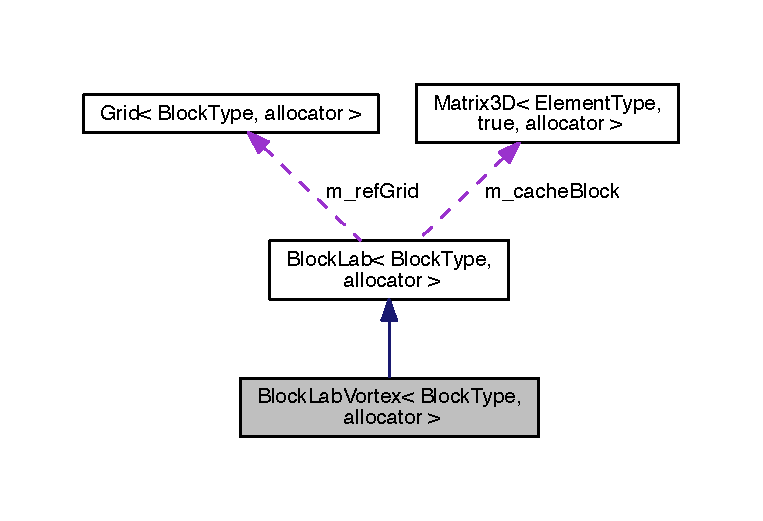
\includegraphics[width=350pt]{de/d72/class_block_lab_vortex__coll__graph}
\end{center}
\end{figure}
\subsection*{Public Member Functions}
\begin{DoxyCompactItemize}
\item 
\hyperlink{class_block_lab_vortex_abc154c7e8150e408b0aa640ccca39677}{Block\+Lab\+Vortex} ()
\item 
void \hyperlink{class_block_lab_vortex_a00b846d813f1048a9afd75330bd17cf6}{\+\_\+apply\+\_\+bc} (const \hyperlink{struct_block_info}{Block\+Info} \&info, const \hyperlink{_h_d_f5_dumper_8h_a445a5f0e2a34c9d97d69a3c2d1957907}{Real} t=0)
\end{DoxyCompactItemize}
\subsection*{Additional Inherited Members}


\subsection{Constructor \& Destructor Documentation}
\hypertarget{class_block_lab_vortex_abc154c7e8150e408b0aa640ccca39677}{}\index{Block\+Lab\+Vortex@{Block\+Lab\+Vortex}!Block\+Lab\+Vortex@{Block\+Lab\+Vortex}}
\index{Block\+Lab\+Vortex@{Block\+Lab\+Vortex}!Block\+Lab\+Vortex@{Block\+Lab\+Vortex}}
\subsubsection[{Block\+Lab\+Vortex}]{\setlength{\rightskip}{0pt plus 5cm}template$<$typename Block\+Type , template$<$ typename X $>$ class allocator = std\+::allocator$>$ {\bf Block\+Lab\+Vortex}$<$ {\bf Block\+Type}, allocator $>$\+::{\bf Block\+Lab\+Vortex} (
\begin{DoxyParamCaption}
{}
\end{DoxyParamCaption}
)\hspace{0.3cm}{\ttfamily [inline]}}\label{class_block_lab_vortex_abc154c7e8150e408b0aa640ccca39677}


\subsection{Member Function Documentation}
\hypertarget{class_block_lab_vortex_a00b846d813f1048a9afd75330bd17cf6}{}\index{Block\+Lab\+Vortex@{Block\+Lab\+Vortex}!\+\_\+apply\+\_\+bc@{\+\_\+apply\+\_\+bc}}
\index{\+\_\+apply\+\_\+bc@{\+\_\+apply\+\_\+bc}!Block\+Lab\+Vortex@{Block\+Lab\+Vortex}}
\subsubsection[{\+\_\+apply\+\_\+bc}]{\setlength{\rightskip}{0pt plus 5cm}template$<$typename Block\+Type , template$<$ typename X $>$ class allocator = std\+::allocator$>$ void {\bf Block\+Lab\+Vortex}$<$ {\bf Block\+Type}, allocator $>$\+::\+\_\+apply\+\_\+bc (
\begin{DoxyParamCaption}
\item[{const {\bf Block\+Info} \&}]{info, }
\item[{const {\bf Real}}]{t = {\ttfamily 0}}
\end{DoxyParamCaption}
)\hspace{0.3cm}{\ttfamily [inline]}, {\ttfamily [virtual]}}\label{class_block_lab_vortex_a00b846d813f1048a9afd75330bd17cf6}


Reimplemented from \hyperlink{class_block_lab_a669ac139b57be4967e5f43bc649a8520}{Block\+Lab$<$ Block\+Type, allocator $>$}.



The documentation for this class was generated from the following file\+:\begin{DoxyCompactItemize}
\item 
/\+Users/cconti/\+Desktop/\+Mounts/\+Brutus\+Home/\+Cubism\+U\+P\+\_\+2\+D/source/\hyperlink{_definitions_8h}{Definitions.\+h}\end{DoxyCompactItemize}

\hypertarget{class_boundary_condition}{}\section{Boundary\+Condition$<$ T\+Block, T\+Element, allocator $>$ Class Template Reference}
\label{class_boundary_condition}\index{Boundary\+Condition$<$ T\+Block, T\+Element, allocator $>$@{Boundary\+Condition$<$ T\+Block, T\+Element, allocator $>$}}


{\ttfamily \#include $<$Boundary\+Conditions.\+h$>$}



Collaboration diagram for Boundary\+Condition$<$ T\+Block, T\+Element, allocator $>$\+:\nopagebreak
\begin{figure}[H]
\begin{center}
\leavevmode
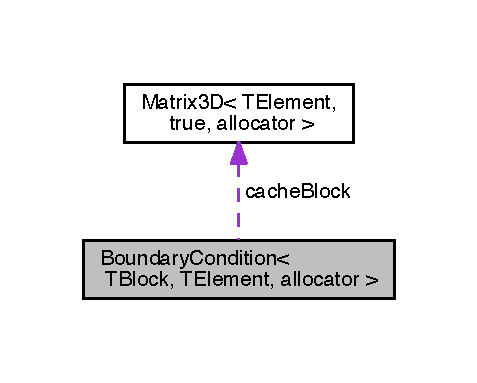
\includegraphics[width=229pt]{d7/d21/class_boundary_condition__coll__graph}
\end{center}
\end{figure}
\subsection*{Public Member Functions}
\begin{DoxyCompactItemize}
\item 
\hyperlink{class_boundary_condition_a89cbd322bff8127af5a49685e3bf04ce}{Boundary\+Condition} (const int ss\mbox{[}3\mbox{]}, const int se\mbox{[}3\mbox{]}, \hyperlink{class_matrix3_d}{Matrix3\+D}$<$ T\+Element, true, allocator $>$ $\ast$\hyperlink{class_boundary_condition_a1e0c33fa794a6d333d4451f8fde04c29}{cache\+Block})
\item 
T\+Element \& \hyperlink{class_boundary_condition_aadcfe05da7761b68191835b09d4d2cf0}{operator()} (int ix, int iy)
\item 
{\footnotesize template$<$int dir, int side$>$ }\\void \hyperlink{class_boundary_condition_adadad3f69ee5cf8ab11dc8f8a7763a4f}{apply\+B\+C\+\_\+dirichlet} (const T\+Element \&p)
\item 
{\footnotesize template$<$int dir, int side$>$ }\\void \hyperlink{class_boundary_condition_a101992951fb756135ca3e44f5d64bb60}{apply\+B\+C\+\_\+neumann} ()
\item 
{\footnotesize template$<$int dir, int side$>$ }\\void \hyperlink{class_boundary_condition_a60e154d33104f42e29dfa49061b266f6}{apply\+B\+C\+\_\+mixed\+Bottom} ()
\item 
{\footnotesize template$<$int dir, int side$>$ }\\void \hyperlink{class_boundary_condition_a77cf65bd542d198d80aa54a3de632ff5}{apply\+B\+C\+\_\+mixed\+Top} ()
\end{DoxyCompactItemize}
\subsection*{Protected Member Functions}
\begin{DoxyCompactItemize}
\item 
{\footnotesize template$<$int dir, int side$>$ }\\void \hyperlink{class_boundary_condition_af8969c6c584388f44cf464a8021d125a}{\+\_\+setup} ()
\end{DoxyCompactItemize}
\subsection*{Protected Attributes}
\begin{DoxyCompactItemize}
\item 
int \hyperlink{class_boundary_condition_a7734cfc6ee1ce3a1dea426ab289a299a}{s} \mbox{[}3\mbox{]}
\item 
int \hyperlink{class_boundary_condition_a755da05bbc5a09adb17a6f1e5a15f25b}{e} \mbox{[}3\mbox{]}
\item 
int \hyperlink{class_boundary_condition_aed1e3cfd20d69c6084d901c246698fdd}{stencil\+Start} \mbox{[}3\mbox{]}
\item 
int \hyperlink{class_boundary_condition_af396b479ba0487ba5c0e45d5b636f09e}{stencil\+End} \mbox{[}3\mbox{]}
\item 
\hyperlink{class_matrix3_d}{Matrix3\+D}$<$ T\+Element, true, allocator $>$ $\ast$ \hyperlink{class_boundary_condition_a1e0c33fa794a6d333d4451f8fde04c29}{cache\+Block}
\end{DoxyCompactItemize}


\subsection{Constructor \& Destructor Documentation}
\hypertarget{class_boundary_condition_a89cbd322bff8127af5a49685e3bf04ce}{}\index{Boundary\+Condition@{Boundary\+Condition}!Boundary\+Condition@{Boundary\+Condition}}
\index{Boundary\+Condition@{Boundary\+Condition}!Boundary\+Condition@{Boundary\+Condition}}
\subsubsection[{Boundary\+Condition}]{\setlength{\rightskip}{0pt plus 5cm}template$<$typename T\+Block, typename T\+Element, template$<$ typename X $>$ class allocator = std\+::allocator$>$ {\bf Boundary\+Condition}$<$ T\+Block, T\+Element, allocator $>$\+::{\bf Boundary\+Condition} (
\begin{DoxyParamCaption}
\item[{const int}]{ss\mbox{[}3\mbox{]}, }
\item[{const int}]{se\mbox{[}3\mbox{]}, }
\item[{{\bf Matrix3\+D}$<$ T\+Element, true, allocator $>$ $\ast$}]{cache\+Block}
\end{DoxyParamCaption}
)\hspace{0.3cm}{\ttfamily [inline]}}\label{class_boundary_condition_a89cbd322bff8127af5a49685e3bf04ce}


\subsection{Member Function Documentation}
\hypertarget{class_boundary_condition_af8969c6c584388f44cf464a8021d125a}{}\index{Boundary\+Condition@{Boundary\+Condition}!\+\_\+setup@{\+\_\+setup}}
\index{\+\_\+setup@{\+\_\+setup}!Boundary\+Condition@{Boundary\+Condition}}
\subsubsection[{\+\_\+setup}]{\setlength{\rightskip}{0pt plus 5cm}template$<$typename T\+Block, typename T\+Element, template$<$ typename X $>$ class allocator = std\+::allocator$>$ template$<$int dir, int side$>$ void {\bf Boundary\+Condition}$<$ T\+Block, T\+Element, allocator $>$\+::\+\_\+setup (
\begin{DoxyParamCaption}
{}
\end{DoxyParamCaption}
)\hspace{0.3cm}{\ttfamily [inline]}, {\ttfamily [protected]}}\label{class_boundary_condition_af8969c6c584388f44cf464a8021d125a}
\hypertarget{class_boundary_condition_adadad3f69ee5cf8ab11dc8f8a7763a4f}{}\index{Boundary\+Condition@{Boundary\+Condition}!apply\+B\+C\+\_\+dirichlet@{apply\+B\+C\+\_\+dirichlet}}
\index{apply\+B\+C\+\_\+dirichlet@{apply\+B\+C\+\_\+dirichlet}!Boundary\+Condition@{Boundary\+Condition}}
\subsubsection[{apply\+B\+C\+\_\+dirichlet}]{\setlength{\rightskip}{0pt plus 5cm}template$<$typename T\+Block, typename T\+Element, template$<$ typename X $>$ class allocator = std\+::allocator$>$ template$<$int dir, int side$>$ void {\bf Boundary\+Condition}$<$ T\+Block, T\+Element, allocator $>$\+::apply\+B\+C\+\_\+dirichlet (
\begin{DoxyParamCaption}
\item[{const T\+Element \&}]{p}
\end{DoxyParamCaption}
)\hspace{0.3cm}{\ttfamily [inline]}}\label{class_boundary_condition_adadad3f69ee5cf8ab11dc8f8a7763a4f}
\hypertarget{class_boundary_condition_a60e154d33104f42e29dfa49061b266f6}{}\index{Boundary\+Condition@{Boundary\+Condition}!apply\+B\+C\+\_\+mixed\+Bottom@{apply\+B\+C\+\_\+mixed\+Bottom}}
\index{apply\+B\+C\+\_\+mixed\+Bottom@{apply\+B\+C\+\_\+mixed\+Bottom}!Boundary\+Condition@{Boundary\+Condition}}
\subsubsection[{apply\+B\+C\+\_\+mixed\+Bottom}]{\setlength{\rightskip}{0pt plus 5cm}template$<$typename T\+Block, typename T\+Element, template$<$ typename X $>$ class allocator = std\+::allocator$>$ template$<$int dir, int side$>$ void {\bf Boundary\+Condition}$<$ T\+Block, T\+Element, allocator $>$\+::apply\+B\+C\+\_\+mixed\+Bottom (
\begin{DoxyParamCaption}
{}
\end{DoxyParamCaption}
)\hspace{0.3cm}{\ttfamily [inline]}}\label{class_boundary_condition_a60e154d33104f42e29dfa49061b266f6}
\hypertarget{class_boundary_condition_a77cf65bd542d198d80aa54a3de632ff5}{}\index{Boundary\+Condition@{Boundary\+Condition}!apply\+B\+C\+\_\+mixed\+Top@{apply\+B\+C\+\_\+mixed\+Top}}
\index{apply\+B\+C\+\_\+mixed\+Top@{apply\+B\+C\+\_\+mixed\+Top}!Boundary\+Condition@{Boundary\+Condition}}
\subsubsection[{apply\+B\+C\+\_\+mixed\+Top}]{\setlength{\rightskip}{0pt plus 5cm}template$<$typename T\+Block, typename T\+Element, template$<$ typename X $>$ class allocator = std\+::allocator$>$ template$<$int dir, int side$>$ void {\bf Boundary\+Condition}$<$ T\+Block, T\+Element, allocator $>$\+::apply\+B\+C\+\_\+mixed\+Top (
\begin{DoxyParamCaption}
{}
\end{DoxyParamCaption}
)\hspace{0.3cm}{\ttfamily [inline]}}\label{class_boundary_condition_a77cf65bd542d198d80aa54a3de632ff5}
\hypertarget{class_boundary_condition_a101992951fb756135ca3e44f5d64bb60}{}\index{Boundary\+Condition@{Boundary\+Condition}!apply\+B\+C\+\_\+neumann@{apply\+B\+C\+\_\+neumann}}
\index{apply\+B\+C\+\_\+neumann@{apply\+B\+C\+\_\+neumann}!Boundary\+Condition@{Boundary\+Condition}}
\subsubsection[{apply\+B\+C\+\_\+neumann}]{\setlength{\rightskip}{0pt plus 5cm}template$<$typename T\+Block, typename T\+Element, template$<$ typename X $>$ class allocator = std\+::allocator$>$ template$<$int dir, int side$>$ void {\bf Boundary\+Condition}$<$ T\+Block, T\+Element, allocator $>$\+::apply\+B\+C\+\_\+neumann (
\begin{DoxyParamCaption}
{}
\end{DoxyParamCaption}
)\hspace{0.3cm}{\ttfamily [inline]}}\label{class_boundary_condition_a101992951fb756135ca3e44f5d64bb60}
\hypertarget{class_boundary_condition_aadcfe05da7761b68191835b09d4d2cf0}{}\index{Boundary\+Condition@{Boundary\+Condition}!operator()@{operator()}}
\index{operator()@{operator()}!Boundary\+Condition@{Boundary\+Condition}}
\subsubsection[{operator()}]{\setlength{\rightskip}{0pt plus 5cm}template$<$typename T\+Block, typename T\+Element, template$<$ typename X $>$ class allocator = std\+::allocator$>$ T\+Element\& {\bf Boundary\+Condition}$<$ T\+Block, T\+Element, allocator $>$\+::operator() (
\begin{DoxyParamCaption}
\item[{int}]{ix, }
\item[{int}]{iy}
\end{DoxyParamCaption}
)\hspace{0.3cm}{\ttfamily [inline]}}\label{class_boundary_condition_aadcfe05da7761b68191835b09d4d2cf0}


Here is the call graph for this function\+:\nopagebreak
\begin{figure}[H]
\begin{center}
\leavevmode
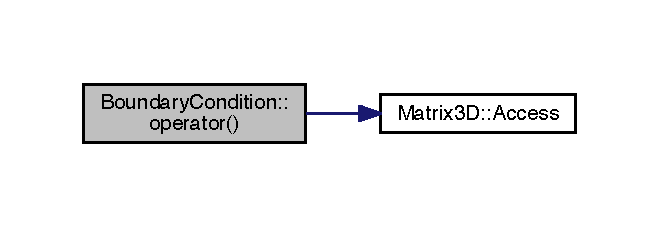
\includegraphics[width=316pt]{db/d64/class_boundary_condition_aadcfe05da7761b68191835b09d4d2cf0_cgraph}
\end{center}
\end{figure}




\subsection{Member Data Documentation}
\hypertarget{class_boundary_condition_a1e0c33fa794a6d333d4451f8fde04c29}{}\index{Boundary\+Condition@{Boundary\+Condition}!cache\+Block@{cache\+Block}}
\index{cache\+Block@{cache\+Block}!Boundary\+Condition@{Boundary\+Condition}}
\subsubsection[{cache\+Block}]{\setlength{\rightskip}{0pt plus 5cm}template$<$typename T\+Block, typename T\+Element, template$<$ typename X $>$ class allocator = std\+::allocator$>$ {\bf Matrix3\+D}$<$T\+Element, true, allocator$>$$\ast$ {\bf Boundary\+Condition}$<$ T\+Block, T\+Element, allocator $>$\+::cache\+Block\hspace{0.3cm}{\ttfamily [protected]}}\label{class_boundary_condition_a1e0c33fa794a6d333d4451f8fde04c29}
\hypertarget{class_boundary_condition_a755da05bbc5a09adb17a6f1e5a15f25b}{}\index{Boundary\+Condition@{Boundary\+Condition}!e@{e}}
\index{e@{e}!Boundary\+Condition@{Boundary\+Condition}}
\subsubsection[{e}]{\setlength{\rightskip}{0pt plus 5cm}template$<$typename T\+Block, typename T\+Element, template$<$ typename X $>$ class allocator = std\+::allocator$>$ int {\bf Boundary\+Condition}$<$ T\+Block, T\+Element, allocator $>$\+::e\mbox{[}3\mbox{]}\hspace{0.3cm}{\ttfamily [protected]}}\label{class_boundary_condition_a755da05bbc5a09adb17a6f1e5a15f25b}
\hypertarget{class_boundary_condition_a7734cfc6ee1ce3a1dea426ab289a299a}{}\index{Boundary\+Condition@{Boundary\+Condition}!s@{s}}
\index{s@{s}!Boundary\+Condition@{Boundary\+Condition}}
\subsubsection[{s}]{\setlength{\rightskip}{0pt plus 5cm}template$<$typename T\+Block, typename T\+Element, template$<$ typename X $>$ class allocator = std\+::allocator$>$ int {\bf Boundary\+Condition}$<$ T\+Block, T\+Element, allocator $>$\+::s\mbox{[}3\mbox{]}\hspace{0.3cm}{\ttfamily [protected]}}\label{class_boundary_condition_a7734cfc6ee1ce3a1dea426ab289a299a}
\hypertarget{class_boundary_condition_af396b479ba0487ba5c0e45d5b636f09e}{}\index{Boundary\+Condition@{Boundary\+Condition}!stencil\+End@{stencil\+End}}
\index{stencil\+End@{stencil\+End}!Boundary\+Condition@{Boundary\+Condition}}
\subsubsection[{stencil\+End}]{\setlength{\rightskip}{0pt plus 5cm}template$<$typename T\+Block, typename T\+Element, template$<$ typename X $>$ class allocator = std\+::allocator$>$ int {\bf Boundary\+Condition}$<$ T\+Block, T\+Element, allocator $>$\+::stencil\+End\mbox{[}3\mbox{]}\hspace{0.3cm}{\ttfamily [protected]}}\label{class_boundary_condition_af396b479ba0487ba5c0e45d5b636f09e}
\hypertarget{class_boundary_condition_aed1e3cfd20d69c6084d901c246698fdd}{}\index{Boundary\+Condition@{Boundary\+Condition}!stencil\+Start@{stencil\+Start}}
\index{stencil\+Start@{stencil\+Start}!Boundary\+Condition@{Boundary\+Condition}}
\subsubsection[{stencil\+Start}]{\setlength{\rightskip}{0pt plus 5cm}template$<$typename T\+Block, typename T\+Element, template$<$ typename X $>$ class allocator = std\+::allocator$>$ int {\bf Boundary\+Condition}$<$ T\+Block, T\+Element, allocator $>$\+::stencil\+Start\mbox{[}3\mbox{]}\hspace{0.3cm}{\ttfamily [protected]}}\label{class_boundary_condition_aed1e3cfd20d69c6084d901c246698fdd}


The documentation for this class was generated from the following file\+:\begin{DoxyCompactItemize}
\item 
source/\hyperlink{_boundary_conditions_8h}{Boundary\+Conditions.\+h}\end{DoxyCompactItemize}

\hypertarget{class_b_s4}{}\section{B\+S4 Class Reference}
\label{class_b_s4}\index{B\+S4@{B\+S4}}
\subsection*{Static Public Member Functions}
\begin{DoxyCompactItemize}
\item 
static \hyperlink{_h_d_f5_dumper_8h_a445a5f0e2a34c9d97d69a3c2d1957907}{Real} \hyperlink{class_b_s4_ab53524385d759ff3e1fafa9b53aee574}{eval} (\hyperlink{_h_d_f5_dumper_8h_a445a5f0e2a34c9d97d69a3c2d1957907}{Real} x)
\item 
static \hyperlink{_h_d_f5_dumper_8h_a445a5f0e2a34c9d97d69a3c2d1957907}{Real} \hyperlink{class_b_s4_ab53524385d759ff3e1fafa9b53aee574}{eval} (\hyperlink{_h_d_f5_dumper_8h_a445a5f0e2a34c9d97d69a3c2d1957907}{Real} x)
\end{DoxyCompactItemize}


\subsection{Member Function Documentation}
\hypertarget{class_b_s4_ab53524385d759ff3e1fafa9b53aee574}{}\index{B\+S4@{B\+S4}!eval@{eval}}
\index{eval@{eval}!B\+S4@{B\+S4}}
\subsubsection[{eval}]{\setlength{\rightskip}{0pt plus 5cm}static {\bf Real} B\+S4\+::eval (
\begin{DoxyParamCaption}
\item[{{\bf Real}}]{x}
\end{DoxyParamCaption}
)\hspace{0.3cm}{\ttfamily [inline]}, {\ttfamily [static]}}\label{class_b_s4_ab53524385d759ff3e1fafa9b53aee574}


Here is the caller graph for this function\+:\nopagebreak
\begin{figure}[H]
\begin{center}
\leavevmode
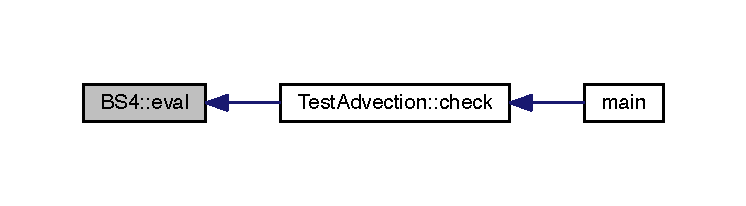
\includegraphics[width=350pt]{d3/d24/class_b_s4_ab53524385d759ff3e1fafa9b53aee574_icgraph}
\end{center}
\end{figure}


\hypertarget{class_b_s4_ab53524385d759ff3e1fafa9b53aee574}{}\index{B\+S4@{B\+S4}!eval@{eval}}
\index{eval@{eval}!B\+S4@{B\+S4}}
\subsubsection[{eval}]{\setlength{\rightskip}{0pt plus 5cm}static {\bf Real} B\+S4\+::eval (
\begin{DoxyParamCaption}
\item[{{\bf Real}}]{x}
\end{DoxyParamCaption}
)\hspace{0.3cm}{\ttfamily [inline]}, {\ttfamily [static]}}\label{class_b_s4_ab53524385d759ff3e1fafa9b53aee574}


The documentation for this class was generated from the following files\+:\begin{DoxyCompactItemize}
\item 
source/\hyperlink{_test_advection_8cpp}{Test\+Advection.\+cpp}\item 
source/\hyperlink{_test_pressure_8cpp}{Test\+Pressure.\+cpp}\end{DoxyCompactItemize}

\hypertarget{class_coordinator_advection}{}\section{Coordinator\+Advection$<$ Lab $>$ Class Template Reference}
\label{class_coordinator_advection}\index{Coordinator\+Advection$<$ Lab $>$@{Coordinator\+Advection$<$ Lab $>$}}


{\ttfamily \#include $<$Coordinator\+Advection.\+h$>$}



Inheritance diagram for Coordinator\+Advection$<$ Lab $>$\+:\nopagebreak
\begin{figure}[H]
\begin{center}
\leavevmode
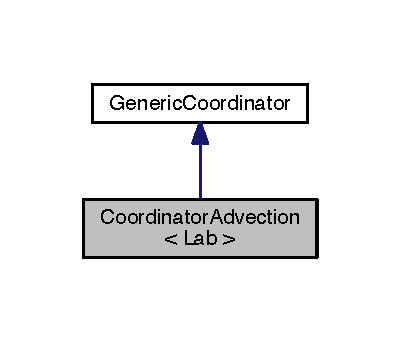
\includegraphics[width=192pt]{d6/d09/class_coordinator_advection__inherit__graph}
\end{center}
\end{figure}


Collaboration diagram for Coordinator\+Advection$<$ Lab $>$\+:\nopagebreak
\begin{figure}[H]
\begin{center}
\leavevmode
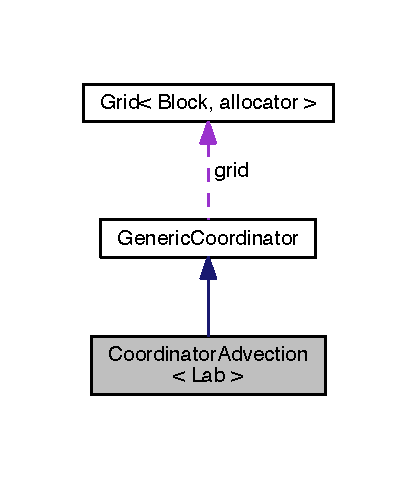
\includegraphics[width=200pt]{de/d4e/class_coordinator_advection__coll__graph}
\end{center}
\end{figure}
\subsection*{Public Member Functions}
\begin{DoxyCompactItemize}
\item 
\hyperlink{class_coordinator_advection_ab8a506c29266c24af3f302d8fbba4229}{Coordinator\+Advection} (\hyperlink{_definitions_8h_aff3288a3741f5098bcc456bb13440189}{Fluid\+Grid} $\ast$\hyperlink{class_generic_coordinator_aa514bbf7394bb5519c6f12daa33a375a}{grid})
\item 
void \hyperlink{class_coordinator_advection_a9cb32410e2cbfcf419138060be504fbb}{operator()} (const double dt)
\item 
\hyperlink{testfpzip_8cpp_a984bb8e04129c4268bd6ff36a50c9fa4}{string} \hyperlink{class_coordinator_advection_a355e311ce03e6a35d2ae78e2cfe129d6}{get\+Name} ()
\end{DoxyCompactItemize}
\subsection*{Protected Member Functions}
\begin{DoxyCompactItemize}
\item 
void \hyperlink{class_coordinator_advection_aafd5d3931db591aebdc52bc8ed3f0ec2}{reset} ()
\item 
void \hyperlink{class_coordinator_advection_a1139ca17fbb50aaf1f21dd6aff0718ba}{update} ()
\item 
void \hyperlink{class_coordinator_advection_a84141dee7184e52394577bbe07838570}{advect} (const double dt)
\end{DoxyCompactItemize}
\subsection*{Additional Inherited Members}


\subsection{Constructor \& Destructor Documentation}
\hypertarget{class_coordinator_advection_ab8a506c29266c24af3f302d8fbba4229}{}\index{Coordinator\+Advection@{Coordinator\+Advection}!Coordinator\+Advection@{Coordinator\+Advection}}
\index{Coordinator\+Advection@{Coordinator\+Advection}!Coordinator\+Advection@{Coordinator\+Advection}}
\subsubsection[{Coordinator\+Advection}]{\setlength{\rightskip}{0pt plus 5cm}template$<$typename Lab $>$ {\bf Coordinator\+Advection}$<$ Lab $>$\+::{\bf Coordinator\+Advection} (
\begin{DoxyParamCaption}
\item[{{\bf Fluid\+Grid} $\ast$}]{grid}
\end{DoxyParamCaption}
)\hspace{0.3cm}{\ttfamily [inline]}}\label{class_coordinator_advection_ab8a506c29266c24af3f302d8fbba4229}


\subsection{Member Function Documentation}
\hypertarget{class_coordinator_advection_a84141dee7184e52394577bbe07838570}{}\index{Coordinator\+Advection@{Coordinator\+Advection}!advect@{advect}}
\index{advect@{advect}!Coordinator\+Advection@{Coordinator\+Advection}}
\subsubsection[{advect}]{\setlength{\rightskip}{0pt plus 5cm}template$<$typename Lab $>$ void {\bf Coordinator\+Advection}$<$ Lab $>$\+::advect (
\begin{DoxyParamCaption}
\item[{const double}]{dt}
\end{DoxyParamCaption}
)\hspace{0.3cm}{\ttfamily [inline]}, {\ttfamily [protected]}}\label{class_coordinator_advection_a84141dee7184e52394577bbe07838570}


Here is the caller graph for this function\+:\nopagebreak
\begin{figure}[H]
\begin{center}
\leavevmode
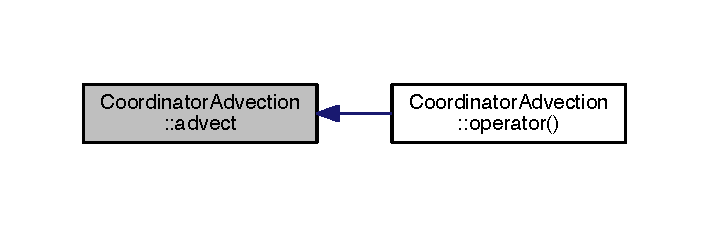
\includegraphics[width=340pt]{d9/d0e/class_coordinator_advection_a84141dee7184e52394577bbe07838570_icgraph}
\end{center}
\end{figure}


\hypertarget{class_coordinator_advection_a355e311ce03e6a35d2ae78e2cfe129d6}{}\index{Coordinator\+Advection@{Coordinator\+Advection}!get\+Name@{get\+Name}}
\index{get\+Name@{get\+Name}!Coordinator\+Advection@{Coordinator\+Advection}}
\subsubsection[{get\+Name}]{\setlength{\rightskip}{0pt plus 5cm}template$<$typename Lab $>$ {\bf string} {\bf Coordinator\+Advection}$<$ Lab $>$\+::get\+Name (
\begin{DoxyParamCaption}
{}
\end{DoxyParamCaption}
)\hspace{0.3cm}{\ttfamily [inline]}, {\ttfamily [virtual]}}\label{class_coordinator_advection_a355e311ce03e6a35d2ae78e2cfe129d6}


Implements \hyperlink{class_generic_coordinator_a8c1b9f4fa96d1c7b851e85e19325de1d}{Generic\+Coordinator}.

\hypertarget{class_coordinator_advection_a9cb32410e2cbfcf419138060be504fbb}{}\index{Coordinator\+Advection@{Coordinator\+Advection}!operator()@{operator()}}
\index{operator()@{operator()}!Coordinator\+Advection@{Coordinator\+Advection}}
\subsubsection[{operator()}]{\setlength{\rightskip}{0pt plus 5cm}template$<$typename Lab $>$ void {\bf Coordinator\+Advection}$<$ Lab $>$\+::operator() (
\begin{DoxyParamCaption}
\item[{const double}]{dt}
\end{DoxyParamCaption}
)\hspace{0.3cm}{\ttfamily [inline]}, {\ttfamily [virtual]}}\label{class_coordinator_advection_a9cb32410e2cbfcf419138060be504fbb}


Implements \hyperlink{class_generic_coordinator_a984696fef63daf7253b87ce21cce3f94}{Generic\+Coordinator}.



Here is the call graph for this function\+:
\nopagebreak
\begin{figure}[H]
\begin{center}
\leavevmode
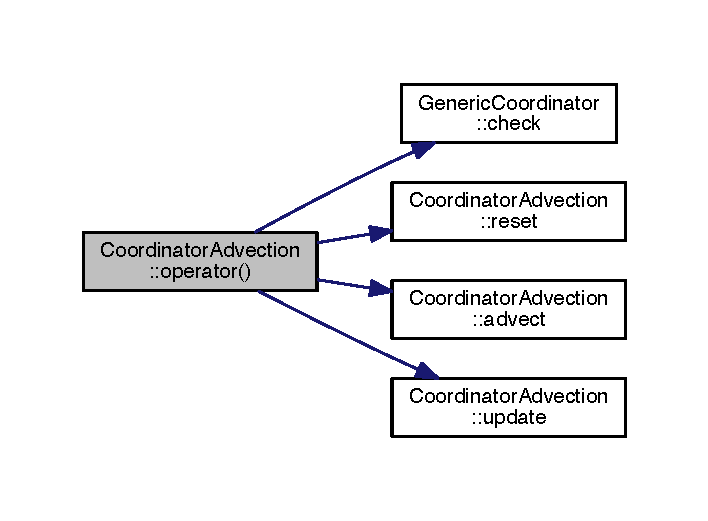
\includegraphics[width=340pt]{d9/d0e/class_coordinator_advection_a9cb32410e2cbfcf419138060be504fbb_cgraph}
\end{center}
\end{figure}


\hypertarget{class_coordinator_advection_aafd5d3931db591aebdc52bc8ed3f0ec2}{}\index{Coordinator\+Advection@{Coordinator\+Advection}!reset@{reset}}
\index{reset@{reset}!Coordinator\+Advection@{Coordinator\+Advection}}
\subsubsection[{reset}]{\setlength{\rightskip}{0pt plus 5cm}template$<$typename Lab $>$ void {\bf Coordinator\+Advection}$<$ Lab $>$\+::reset (
\begin{DoxyParamCaption}
{}
\end{DoxyParamCaption}
)\hspace{0.3cm}{\ttfamily [inline]}, {\ttfamily [protected]}}\label{class_coordinator_advection_aafd5d3931db591aebdc52bc8ed3f0ec2}


Here is the caller graph for this function\+:\nopagebreak
\begin{figure}[H]
\begin{center}
\leavevmode
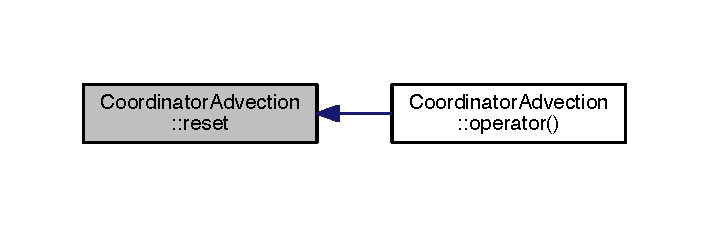
\includegraphics[width=340pt]{d9/d0e/class_coordinator_advection_aafd5d3931db591aebdc52bc8ed3f0ec2_icgraph}
\end{center}
\end{figure}


\hypertarget{class_coordinator_advection_a1139ca17fbb50aaf1f21dd6aff0718ba}{}\index{Coordinator\+Advection@{Coordinator\+Advection}!update@{update}}
\index{update@{update}!Coordinator\+Advection@{Coordinator\+Advection}}
\subsubsection[{update}]{\setlength{\rightskip}{0pt plus 5cm}template$<$typename Lab $>$ void {\bf Coordinator\+Advection}$<$ Lab $>$\+::update (
\begin{DoxyParamCaption}
{}
\end{DoxyParamCaption}
)\hspace{0.3cm}{\ttfamily [inline]}, {\ttfamily [protected]}}\label{class_coordinator_advection_a1139ca17fbb50aaf1f21dd6aff0718ba}


Here is the caller graph for this function\+:\nopagebreak
\begin{figure}[H]
\begin{center}
\leavevmode
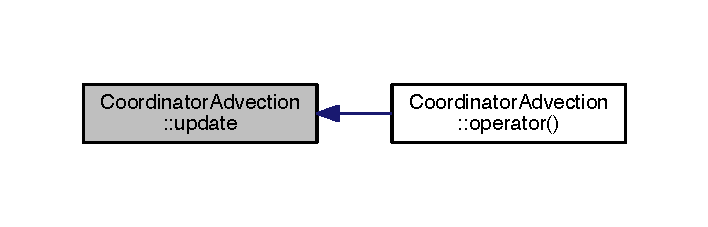
\includegraphics[width=340pt]{d9/d0e/class_coordinator_advection_a1139ca17fbb50aaf1f21dd6aff0718ba_icgraph}
\end{center}
\end{figure}




The documentation for this class was generated from the following file\+:\begin{DoxyCompactItemize}
\item 
/\+Users/cconti/\+Desktop/\+Mounts/\+Brutus\+Home/\+Cubism\+U\+P\+\_\+2\+D/source/\hyperlink{_coordinator_advection_8h}{Coordinator\+Advection.\+h}\end{DoxyCompactItemize}

\hypertarget{class_coordinator_body_velocities}{}\section{Coordinator\+Body\+Velocities Class Reference}
\label{class_coordinator_body_velocities}\index{Coordinator\+Body\+Velocities@{Coordinator\+Body\+Velocities}}


{\ttfamily \#include $<$Coordinator\+Body\+Velocities.\+h$>$}



Inheritance diagram for Coordinator\+Body\+Velocities\+:\nopagebreak
\begin{figure}[H]
\begin{center}
\leavevmode
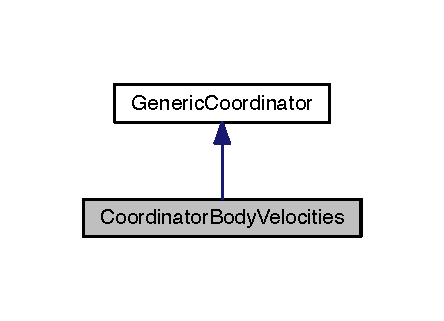
\includegraphics[width=213pt]{dc/d0c/class_coordinator_body_velocities__inherit__graph}
\end{center}
\end{figure}


Collaboration diagram for Coordinator\+Body\+Velocities\+:\nopagebreak
\begin{figure}[H]
\begin{center}
\leavevmode
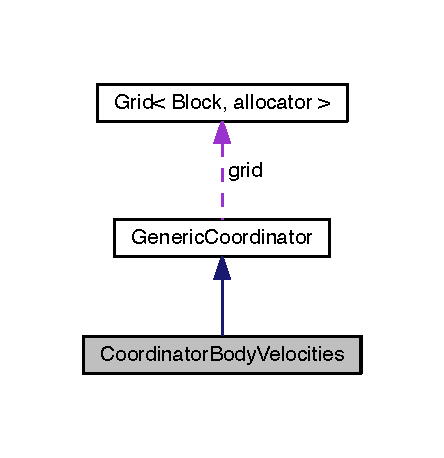
\includegraphics[width=213pt]{d4/d7e/class_coordinator_body_velocities__coll__graph}
\end{center}
\end{figure}
\subsection*{Public Member Functions}
\begin{DoxyCompactItemize}
\item 
\hyperlink{class_coordinator_body_velocities_a24039137e6024c160f253a0c5e7ffa8c}{Coordinator\+Body\+Velocities} (\hyperlink{_h_d_f5_dumper_8h_a445a5f0e2a34c9d97d69a3c2d1957907}{Real} $\ast$\hyperlink{class_coordinator_body_velocities_ad44f24f272833d8f8958ea945543eff6}{u\+Body}, \hyperlink{_h_d_f5_dumper_8h_a445a5f0e2a34c9d97d69a3c2d1957907}{Real} $\ast$\hyperlink{class_coordinator_body_velocities_a5802af8438271a7ee6253f2a1c0695c4}{v\+Body}, \hyperlink{_h_d_f5_dumper_8h_a445a5f0e2a34c9d97d69a3c2d1957907}{Real} $\ast$\hyperlink{class_coordinator_body_velocities_a90b12064de38ba17d4d66198e73ffcbf}{omega\+Body}, const \hyperlink{_h_d_f5_dumper_8h_a445a5f0e2a34c9d97d69a3c2d1957907}{Real} \hyperlink{class_coordinator_body_velocities_afd8b8760d3e9f7fe256ced94c5c8ba15}{lambda}, \hyperlink{_definitions_8h_aff3288a3741f5098bcc456bb13440189}{Fluid\+Grid} $\ast$\hyperlink{class_generic_coordinator_aa514bbf7394bb5519c6f12daa33a375a}{grid})
\item 
void \hyperlink{class_coordinator_body_velocities_a0026fe01ababb24ef5918bca94421043}{operator()} (const double dt)
\item 
\hyperlink{testfpzip_8cpp_a984bb8e04129c4268bd6ff36a50c9fa4}{string} \hyperlink{class_coordinator_body_velocities_a5ba0919947f35c42da51c513ac6a610c}{get\+Name} ()
\end{DoxyCompactItemize}
\subsection*{Protected Attributes}
\begin{DoxyCompactItemize}
\item 
\hyperlink{_h_d_f5_dumper_8h_a445a5f0e2a34c9d97d69a3c2d1957907}{Real} $\ast$ \hyperlink{class_coordinator_body_velocities_ad44f24f272833d8f8958ea945543eff6}{u\+Body}
\item 
\hyperlink{_h_d_f5_dumper_8h_a445a5f0e2a34c9d97d69a3c2d1957907}{Real} $\ast$ \hyperlink{class_coordinator_body_velocities_a5802af8438271a7ee6253f2a1c0695c4}{v\+Body}
\item 
\hyperlink{_h_d_f5_dumper_8h_a445a5f0e2a34c9d97d69a3c2d1957907}{Real} $\ast$ \hyperlink{class_coordinator_body_velocities_a90b12064de38ba17d4d66198e73ffcbf}{omega\+Body}
\item 
\hyperlink{_h_d_f5_dumper_8h_a445a5f0e2a34c9d97d69a3c2d1957907}{Real} \hyperlink{class_coordinator_body_velocities_afd8b8760d3e9f7fe256ced94c5c8ba15}{lambda}
\end{DoxyCompactItemize}
\subsection*{Additional Inherited Members}


\subsection{Constructor \& Destructor Documentation}
\hypertarget{class_coordinator_body_velocities_a24039137e6024c160f253a0c5e7ffa8c}{}\index{Coordinator\+Body\+Velocities@{Coordinator\+Body\+Velocities}!Coordinator\+Body\+Velocities@{Coordinator\+Body\+Velocities}}
\index{Coordinator\+Body\+Velocities@{Coordinator\+Body\+Velocities}!Coordinator\+Body\+Velocities@{Coordinator\+Body\+Velocities}}
\subsubsection[{Coordinator\+Body\+Velocities}]{\setlength{\rightskip}{0pt plus 5cm}Coordinator\+Body\+Velocities\+::\+Coordinator\+Body\+Velocities (
\begin{DoxyParamCaption}
\item[{{\bf Real} $\ast$}]{u\+Body, }
\item[{{\bf Real} $\ast$}]{v\+Body, }
\item[{{\bf Real} $\ast$}]{omega\+Body, }
\item[{const {\bf Real}}]{lambda, }
\item[{{\bf Fluid\+Grid} $\ast$}]{grid}
\end{DoxyParamCaption}
)\hspace{0.3cm}{\ttfamily [inline]}}\label{class_coordinator_body_velocities_a24039137e6024c160f253a0c5e7ffa8c}


\subsection{Member Function Documentation}
\hypertarget{class_coordinator_body_velocities_a5ba0919947f35c42da51c513ac6a610c}{}\index{Coordinator\+Body\+Velocities@{Coordinator\+Body\+Velocities}!get\+Name@{get\+Name}}
\index{get\+Name@{get\+Name}!Coordinator\+Body\+Velocities@{Coordinator\+Body\+Velocities}}
\subsubsection[{get\+Name}]{\setlength{\rightskip}{0pt plus 5cm}{\bf string} Coordinator\+Body\+Velocities\+::get\+Name (
\begin{DoxyParamCaption}
{}
\end{DoxyParamCaption}
)\hspace{0.3cm}{\ttfamily [inline]}, {\ttfamily [virtual]}}\label{class_coordinator_body_velocities_a5ba0919947f35c42da51c513ac6a610c}


Implements \hyperlink{class_generic_coordinator_a8c1b9f4fa96d1c7b851e85e19325de1d}{Generic\+Coordinator}.

\hypertarget{class_coordinator_body_velocities_a0026fe01ababb24ef5918bca94421043}{}\index{Coordinator\+Body\+Velocities@{Coordinator\+Body\+Velocities}!operator()@{operator()}}
\index{operator()@{operator()}!Coordinator\+Body\+Velocities@{Coordinator\+Body\+Velocities}}
\subsubsection[{operator()}]{\setlength{\rightskip}{0pt plus 5cm}void Coordinator\+Body\+Velocities\+::operator() (
\begin{DoxyParamCaption}
\item[{const double}]{dt}
\end{DoxyParamCaption}
)\hspace{0.3cm}{\ttfamily [inline]}, {\ttfamily [virtual]}}\label{class_coordinator_body_velocities_a0026fe01ababb24ef5918bca94421043}


Implements \hyperlink{class_generic_coordinator_a984696fef63daf7253b87ce21cce3f94}{Generic\+Coordinator}.



Here is the call graph for this function\+:\nopagebreak
\begin{figure}[H]
\begin{center}
\leavevmode
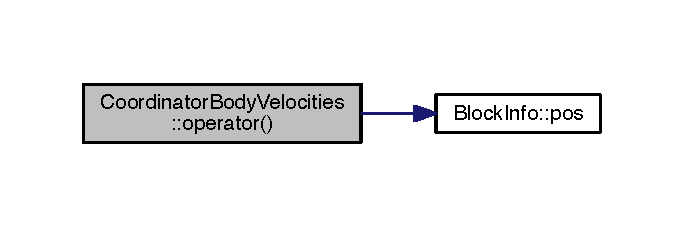
\includegraphics[width=328pt]{d9/ddd/class_coordinator_body_velocities_a0026fe01ababb24ef5918bca94421043_cgraph}
\end{center}
\end{figure}




\subsection{Member Data Documentation}
\hypertarget{class_coordinator_body_velocities_afd8b8760d3e9f7fe256ced94c5c8ba15}{}\index{Coordinator\+Body\+Velocities@{Coordinator\+Body\+Velocities}!lambda@{lambda}}
\index{lambda@{lambda}!Coordinator\+Body\+Velocities@{Coordinator\+Body\+Velocities}}
\subsubsection[{lambda}]{\setlength{\rightskip}{0pt plus 5cm}{\bf Real} Coordinator\+Body\+Velocities\+::lambda\hspace{0.3cm}{\ttfamily [protected]}}\label{class_coordinator_body_velocities_afd8b8760d3e9f7fe256ced94c5c8ba15}
\hypertarget{class_coordinator_body_velocities_a90b12064de38ba17d4d66198e73ffcbf}{}\index{Coordinator\+Body\+Velocities@{Coordinator\+Body\+Velocities}!omega\+Body@{omega\+Body}}
\index{omega\+Body@{omega\+Body}!Coordinator\+Body\+Velocities@{Coordinator\+Body\+Velocities}}
\subsubsection[{omega\+Body}]{\setlength{\rightskip}{0pt plus 5cm}{\bf Real} $\ast$ Coordinator\+Body\+Velocities\+::omega\+Body\hspace{0.3cm}{\ttfamily [protected]}}\label{class_coordinator_body_velocities_a90b12064de38ba17d4d66198e73ffcbf}
\hypertarget{class_coordinator_body_velocities_ad44f24f272833d8f8958ea945543eff6}{}\index{Coordinator\+Body\+Velocities@{Coordinator\+Body\+Velocities}!u\+Body@{u\+Body}}
\index{u\+Body@{u\+Body}!Coordinator\+Body\+Velocities@{Coordinator\+Body\+Velocities}}
\subsubsection[{u\+Body}]{\setlength{\rightskip}{0pt plus 5cm}{\bf Real}$\ast$ Coordinator\+Body\+Velocities\+::u\+Body\hspace{0.3cm}{\ttfamily [protected]}}\label{class_coordinator_body_velocities_ad44f24f272833d8f8958ea945543eff6}
\hypertarget{class_coordinator_body_velocities_a5802af8438271a7ee6253f2a1c0695c4}{}\index{Coordinator\+Body\+Velocities@{Coordinator\+Body\+Velocities}!v\+Body@{v\+Body}}
\index{v\+Body@{v\+Body}!Coordinator\+Body\+Velocities@{Coordinator\+Body\+Velocities}}
\subsubsection[{v\+Body}]{\setlength{\rightskip}{0pt plus 5cm}{\bf Real} $\ast$ Coordinator\+Body\+Velocities\+::v\+Body\hspace{0.3cm}{\ttfamily [protected]}}\label{class_coordinator_body_velocities_a5802af8438271a7ee6253f2a1c0695c4}


The documentation for this class was generated from the following file\+:\begin{DoxyCompactItemize}
\item 
/\+Users/cconti/\+Desktop/\+Mounts/\+Brutus\+Home/\+Cubism\+U\+P\+\_\+2\+D/source/\hyperlink{_coordinator_body_velocities_8h}{Coordinator\+Body\+Velocities.\+h}\end{DoxyCompactItemize}

\hypertarget{class_coordinator_compute_shape}{}\section{Coordinator\+Compute\+Shape Class Reference}
\label{class_coordinator_compute_shape}\index{Coordinator\+Compute\+Shape@{Coordinator\+Compute\+Shape}}


{\ttfamily \#include $<$Coordinator\+Compute\+Shape.\+h$>$}



Inheritance diagram for Coordinator\+Compute\+Shape\+:\nopagebreak
\begin{figure}[H]
\begin{center}
\leavevmode
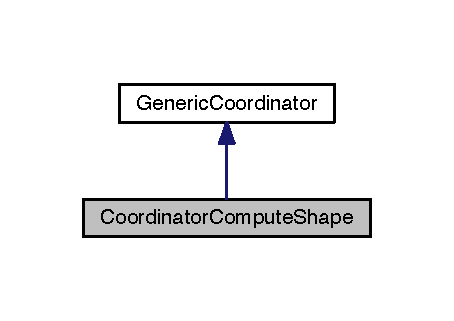
\includegraphics[width=218pt]{dd/d53/class_coordinator_compute_shape__inherit__graph}
\end{center}
\end{figure}


Collaboration diagram for Coordinator\+Compute\+Shape\+:\nopagebreak
\begin{figure}[H]
\begin{center}
\leavevmode
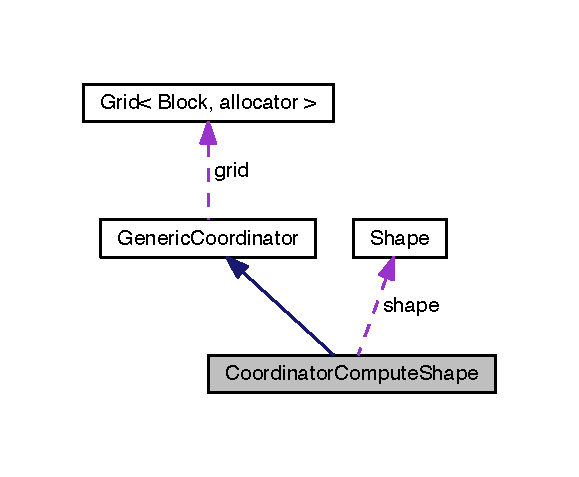
\includegraphics[width=278pt]{df/dcf/class_coordinator_compute_shape__coll__graph}
\end{center}
\end{figure}
\subsection*{Public Member Functions}
\begin{DoxyCompactItemize}
\item 
\hyperlink{class_coordinator_compute_shape_abbd719f8faf9f24f1ed88cf4e5151b46}{Coordinator\+Compute\+Shape} (\hyperlink{_h_d_f5_dumper_8h_a445a5f0e2a34c9d97d69a3c2d1957907}{Real} $\ast$\hyperlink{class_coordinator_compute_shape_adc09b276b152cb1efd9ce1af98f7642a}{u\+Body}, \hyperlink{_h_d_f5_dumper_8h_a445a5f0e2a34c9d97d69a3c2d1957907}{Real} $\ast$\hyperlink{class_coordinator_compute_shape_ae4f0f03770ea60b05034bd0a1fdddf45}{v\+Body}, \hyperlink{_h_d_f5_dumper_8h_a445a5f0e2a34c9d97d69a3c2d1957907}{Real} $\ast$\hyperlink{class_coordinator_compute_shape_ad8fc7ad631324607d5d887d7c79ae0b7}{omega\+Body}, \hyperlink{class_shape}{Shape} $\ast$\hyperlink{class_coordinator_compute_shape_a0a772cc3cb7014cdf9f271b3b4792a3c}{shape}, \hyperlink{_definitions_8h_aff3288a3741f5098bcc456bb13440189}{Fluid\+Grid} $\ast$\hyperlink{class_generic_coordinator_aa514bbf7394bb5519c6f12daa33a375a}{grid})
\item 
void \hyperlink{class_coordinator_compute_shape_a3c3eb6c738617c70ba72a74fe8a10038}{operator()} (const double dt)
\item 
\hyperlink{testfpzip_8cpp_a984bb8e04129c4268bd6ff36a50c9fa4}{string} \hyperlink{class_coordinator_compute_shape_a13134ee7d7f1fa7f39da8122e788e048}{get\+Name} ()
\end{DoxyCompactItemize}
\subsection*{Protected Attributes}
\begin{DoxyCompactItemize}
\item 
\hyperlink{_h_d_f5_dumper_8h_a445a5f0e2a34c9d97d69a3c2d1957907}{Real} $\ast$ \hyperlink{class_coordinator_compute_shape_adc09b276b152cb1efd9ce1af98f7642a}{u\+Body}
\item 
\hyperlink{_h_d_f5_dumper_8h_a445a5f0e2a34c9d97d69a3c2d1957907}{Real} $\ast$ \hyperlink{class_coordinator_compute_shape_ae4f0f03770ea60b05034bd0a1fdddf45}{v\+Body}
\item 
\hyperlink{_h_d_f5_dumper_8h_a445a5f0e2a34c9d97d69a3c2d1957907}{Real} $\ast$ \hyperlink{class_coordinator_compute_shape_ad8fc7ad631324607d5d887d7c79ae0b7}{omega\+Body}
\item 
\hyperlink{class_shape}{Shape} $\ast$ \hyperlink{class_coordinator_compute_shape_a0a772cc3cb7014cdf9f271b3b4792a3c}{shape}
\end{DoxyCompactItemize}
\subsection*{Additional Inherited Members}


\subsection{Constructor \& Destructor Documentation}
\hypertarget{class_coordinator_compute_shape_abbd719f8faf9f24f1ed88cf4e5151b46}{}\index{Coordinator\+Compute\+Shape@{Coordinator\+Compute\+Shape}!Coordinator\+Compute\+Shape@{Coordinator\+Compute\+Shape}}
\index{Coordinator\+Compute\+Shape@{Coordinator\+Compute\+Shape}!Coordinator\+Compute\+Shape@{Coordinator\+Compute\+Shape}}
\subsubsection[{Coordinator\+Compute\+Shape}]{\setlength{\rightskip}{0pt plus 5cm}Coordinator\+Compute\+Shape\+::\+Coordinator\+Compute\+Shape (
\begin{DoxyParamCaption}
\item[{{\bf Real} $\ast$}]{u\+Body, }
\item[{{\bf Real} $\ast$}]{v\+Body, }
\item[{{\bf Real} $\ast$}]{omega\+Body, }
\item[{{\bf Shape} $\ast$}]{shape, }
\item[{{\bf Fluid\+Grid} $\ast$}]{grid}
\end{DoxyParamCaption}
)\hspace{0.3cm}{\ttfamily [inline]}}\label{class_coordinator_compute_shape_abbd719f8faf9f24f1ed88cf4e5151b46}


\subsection{Member Function Documentation}
\hypertarget{class_coordinator_compute_shape_a13134ee7d7f1fa7f39da8122e788e048}{}\index{Coordinator\+Compute\+Shape@{Coordinator\+Compute\+Shape}!get\+Name@{get\+Name}}
\index{get\+Name@{get\+Name}!Coordinator\+Compute\+Shape@{Coordinator\+Compute\+Shape}}
\subsubsection[{get\+Name}]{\setlength{\rightskip}{0pt plus 5cm}{\bf string} Coordinator\+Compute\+Shape\+::get\+Name (
\begin{DoxyParamCaption}
{}
\end{DoxyParamCaption}
)\hspace{0.3cm}{\ttfamily [inline]}, {\ttfamily [virtual]}}\label{class_coordinator_compute_shape_a13134ee7d7f1fa7f39da8122e788e048}


Implements \hyperlink{class_generic_coordinator_a8c1b9f4fa96d1c7b851e85e19325de1d}{Generic\+Coordinator}.

\hypertarget{class_coordinator_compute_shape_a3c3eb6c738617c70ba72a74fe8a10038}{}\index{Coordinator\+Compute\+Shape@{Coordinator\+Compute\+Shape}!operator()@{operator()}}
\index{operator()@{operator()}!Coordinator\+Compute\+Shape@{Coordinator\+Compute\+Shape}}
\subsubsection[{operator()}]{\setlength{\rightskip}{0pt plus 5cm}void Coordinator\+Compute\+Shape\+::operator() (
\begin{DoxyParamCaption}
\item[{const double}]{dt}
\end{DoxyParamCaption}
)\hspace{0.3cm}{\ttfamily [inline]}, {\ttfamily [virtual]}}\label{class_coordinator_compute_shape_a3c3eb6c738617c70ba72a74fe8a10038}


Implements \hyperlink{class_generic_coordinator_a984696fef63daf7253b87ce21cce3f94}{Generic\+Coordinator}.



Here is the call graph for this function\+:\nopagebreak
\begin{figure}[H]
\begin{center}
\leavevmode
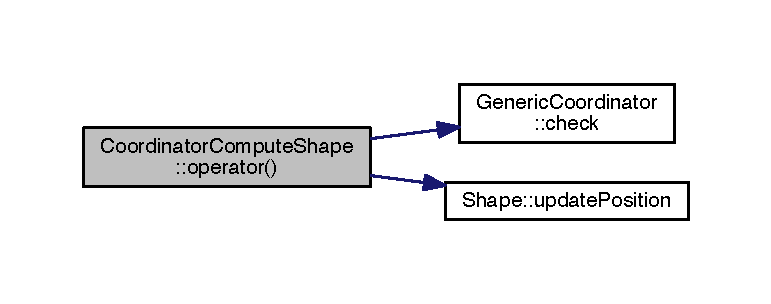
\includegraphics[width=350pt]{d6/d6e/class_coordinator_compute_shape_a3c3eb6c738617c70ba72a74fe8a10038_cgraph}
\end{center}
\end{figure}




\subsection{Member Data Documentation}
\hypertarget{class_coordinator_compute_shape_ad8fc7ad631324607d5d887d7c79ae0b7}{}\index{Coordinator\+Compute\+Shape@{Coordinator\+Compute\+Shape}!omega\+Body@{omega\+Body}}
\index{omega\+Body@{omega\+Body}!Coordinator\+Compute\+Shape@{Coordinator\+Compute\+Shape}}
\subsubsection[{omega\+Body}]{\setlength{\rightskip}{0pt plus 5cm}{\bf Real} $\ast$ Coordinator\+Compute\+Shape\+::omega\+Body\hspace{0.3cm}{\ttfamily [protected]}}\label{class_coordinator_compute_shape_ad8fc7ad631324607d5d887d7c79ae0b7}
\hypertarget{class_coordinator_compute_shape_a0a772cc3cb7014cdf9f271b3b4792a3c}{}\index{Coordinator\+Compute\+Shape@{Coordinator\+Compute\+Shape}!shape@{shape}}
\index{shape@{shape}!Coordinator\+Compute\+Shape@{Coordinator\+Compute\+Shape}}
\subsubsection[{shape}]{\setlength{\rightskip}{0pt plus 5cm}{\bf Shape}$\ast$ Coordinator\+Compute\+Shape\+::shape\hspace{0.3cm}{\ttfamily [protected]}}\label{class_coordinator_compute_shape_a0a772cc3cb7014cdf9f271b3b4792a3c}
\hypertarget{class_coordinator_compute_shape_adc09b276b152cb1efd9ce1af98f7642a}{}\index{Coordinator\+Compute\+Shape@{Coordinator\+Compute\+Shape}!u\+Body@{u\+Body}}
\index{u\+Body@{u\+Body}!Coordinator\+Compute\+Shape@{Coordinator\+Compute\+Shape}}
\subsubsection[{u\+Body}]{\setlength{\rightskip}{0pt plus 5cm}{\bf Real}$\ast$ Coordinator\+Compute\+Shape\+::u\+Body\hspace{0.3cm}{\ttfamily [protected]}}\label{class_coordinator_compute_shape_adc09b276b152cb1efd9ce1af98f7642a}
\hypertarget{class_coordinator_compute_shape_ae4f0f03770ea60b05034bd0a1fdddf45}{}\index{Coordinator\+Compute\+Shape@{Coordinator\+Compute\+Shape}!v\+Body@{v\+Body}}
\index{v\+Body@{v\+Body}!Coordinator\+Compute\+Shape@{Coordinator\+Compute\+Shape}}
\subsubsection[{v\+Body}]{\setlength{\rightskip}{0pt plus 5cm}{\bf Real} $\ast$ Coordinator\+Compute\+Shape\+::v\+Body\hspace{0.3cm}{\ttfamily [protected]}}\label{class_coordinator_compute_shape_ae4f0f03770ea60b05034bd0a1fdddf45}


The documentation for this class was generated from the following file\+:\begin{DoxyCompactItemize}
\item 
/\+Users/cconti/\+Desktop/\+Mounts/\+Brutus\+Home/\+Cubism\+U\+P\+\_\+2\+D/source/\hyperlink{_coordinator_compute_shape_8h}{Coordinator\+Compute\+Shape.\+h}\end{DoxyCompactItemize}

\hypertarget{class_coordinator_diffusion}{}\section{Coordinator\+Diffusion$<$ Lab $>$ Class Template Reference}
\label{class_coordinator_diffusion}\index{Coordinator\+Diffusion$<$ Lab $>$@{Coordinator\+Diffusion$<$ Lab $>$}}


{\ttfamily \#include $<$Coordinator\+Diffusion.\+h$>$}



Inheritance diagram for Coordinator\+Diffusion$<$ Lab $>$\+:\nopagebreak
\begin{figure}[H]
\begin{center}
\leavevmode
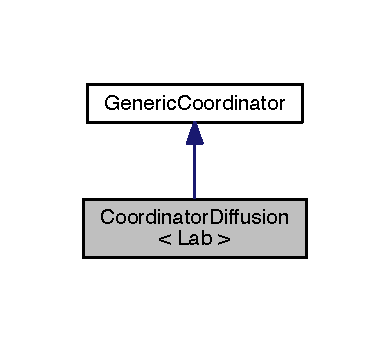
\includegraphics[width=187pt]{d5/db2/class_coordinator_diffusion__inherit__graph}
\end{center}
\end{figure}


Collaboration diagram for Coordinator\+Diffusion$<$ Lab $>$\+:\nopagebreak
\begin{figure}[H]
\begin{center}
\leavevmode
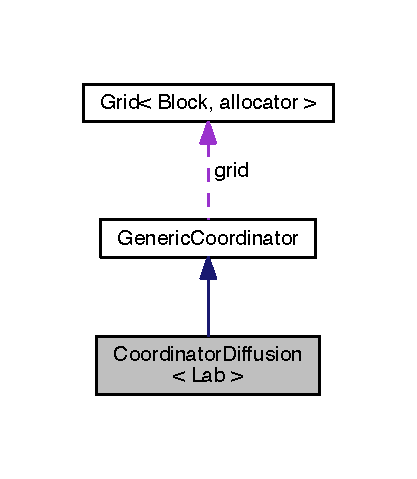
\includegraphics[width=200pt]{d5/d24/class_coordinator_diffusion__coll__graph}
\end{center}
\end{figure}
\subsection*{Public Member Functions}
\begin{DoxyCompactItemize}
\item 
\hyperlink{class_coordinator_diffusion_acd96f26a0bc606db956886cc77d7b4fa}{Coordinator\+Diffusion} (const double \hyperlink{class_coordinator_diffusion_a8e1ee974d96ba320f26bcf7197e959fe}{coeff}, \hyperlink{_definitions_8h_aff3288a3741f5098bcc456bb13440189}{Fluid\+Grid} $\ast$\hyperlink{class_generic_coordinator_aa514bbf7394bb5519c6f12daa33a375a}{grid})
\item 
void \hyperlink{class_coordinator_diffusion_a110e64039f79bcc6f0bfd430cb1f8c53}{operator()} (const double dt)
\item 
\hyperlink{testfpzip_8cpp_a984bb8e04129c4268bd6ff36a50c9fa4}{string} \hyperlink{class_coordinator_diffusion_ae06bddc3554895dbd7ebdf9218dfbd20}{get\+Name} ()
\end{DoxyCompactItemize}
\subsection*{Protected Member Functions}
\begin{DoxyCompactItemize}
\item 
void \hyperlink{class_coordinator_diffusion_a496dde2de4c2ca2fe4d19dad33d2e93e}{reset} ()
\item 
void \hyperlink{class_coordinator_diffusion_aa3c7fd1a3955f9f5358e093b296992a0}{update} ()
\item 
void \hyperlink{class_coordinator_diffusion_ae80d7775fcabdcd9934262ff2c7cf1b5}{diffuse} (const double dt, const int stage)
\end{DoxyCompactItemize}
\subsection*{Protected Attributes}
\begin{DoxyCompactItemize}
\item 
const double \hyperlink{class_coordinator_diffusion_a8e1ee974d96ba320f26bcf7197e959fe}{coeff}
\end{DoxyCompactItemize}


\subsection{Constructor \& Destructor Documentation}
\hypertarget{class_coordinator_diffusion_acd96f26a0bc606db956886cc77d7b4fa}{}\index{Coordinator\+Diffusion@{Coordinator\+Diffusion}!Coordinator\+Diffusion@{Coordinator\+Diffusion}}
\index{Coordinator\+Diffusion@{Coordinator\+Diffusion}!Coordinator\+Diffusion@{Coordinator\+Diffusion}}
\subsubsection[{Coordinator\+Diffusion}]{\setlength{\rightskip}{0pt plus 5cm}template$<$typename Lab$>$ {\bf Coordinator\+Diffusion}$<$ Lab $>$\+::{\bf Coordinator\+Diffusion} (
\begin{DoxyParamCaption}
\item[{const double}]{coeff, }
\item[{{\bf Fluid\+Grid} $\ast$}]{grid}
\end{DoxyParamCaption}
)\hspace{0.3cm}{\ttfamily [inline]}}\label{class_coordinator_diffusion_acd96f26a0bc606db956886cc77d7b4fa}


\subsection{Member Function Documentation}
\hypertarget{class_coordinator_diffusion_ae80d7775fcabdcd9934262ff2c7cf1b5}{}\index{Coordinator\+Diffusion@{Coordinator\+Diffusion}!diffuse@{diffuse}}
\index{diffuse@{diffuse}!Coordinator\+Diffusion@{Coordinator\+Diffusion}}
\subsubsection[{diffuse}]{\setlength{\rightskip}{0pt plus 5cm}template$<$typename Lab$>$ void {\bf Coordinator\+Diffusion}$<$ Lab $>$\+::diffuse (
\begin{DoxyParamCaption}
\item[{const double}]{dt, }
\item[{const int}]{stage}
\end{DoxyParamCaption}
)\hspace{0.3cm}{\ttfamily [inline]}, {\ttfamily [protected]}}\label{class_coordinator_diffusion_ae80d7775fcabdcd9934262ff2c7cf1b5}


Here is the caller graph for this function\+:\nopagebreak
\begin{figure}[H]
\begin{center}
\leavevmode
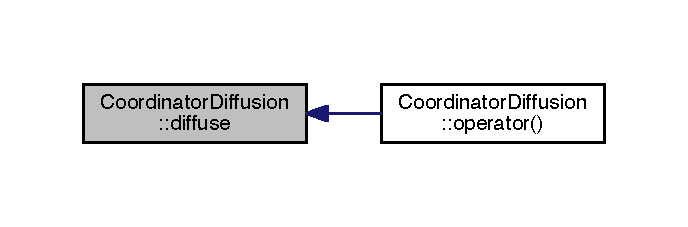
\includegraphics[width=330pt]{d3/dd2/class_coordinator_diffusion_ae80d7775fcabdcd9934262ff2c7cf1b5_icgraph}
\end{center}
\end{figure}


\hypertarget{class_coordinator_diffusion_ae06bddc3554895dbd7ebdf9218dfbd20}{}\index{Coordinator\+Diffusion@{Coordinator\+Diffusion}!get\+Name@{get\+Name}}
\index{get\+Name@{get\+Name}!Coordinator\+Diffusion@{Coordinator\+Diffusion}}
\subsubsection[{get\+Name}]{\setlength{\rightskip}{0pt plus 5cm}template$<$typename Lab$>$ {\bf string} {\bf Coordinator\+Diffusion}$<$ Lab $>$\+::get\+Name (
\begin{DoxyParamCaption}
{}
\end{DoxyParamCaption}
)\hspace{0.3cm}{\ttfamily [inline]}, {\ttfamily [virtual]}}\label{class_coordinator_diffusion_ae06bddc3554895dbd7ebdf9218dfbd20}


Implements \hyperlink{class_generic_coordinator_a8c1b9f4fa96d1c7b851e85e19325de1d}{Generic\+Coordinator}.

\hypertarget{class_coordinator_diffusion_a110e64039f79bcc6f0bfd430cb1f8c53}{}\index{Coordinator\+Diffusion@{Coordinator\+Diffusion}!operator()@{operator()}}
\index{operator()@{operator()}!Coordinator\+Diffusion@{Coordinator\+Diffusion}}
\subsubsection[{operator()}]{\setlength{\rightskip}{0pt plus 5cm}template$<$typename Lab$>$ void {\bf Coordinator\+Diffusion}$<$ Lab $>$\+::operator() (
\begin{DoxyParamCaption}
\item[{const double}]{dt}
\end{DoxyParamCaption}
)\hspace{0.3cm}{\ttfamily [inline]}, {\ttfamily [virtual]}}\label{class_coordinator_diffusion_a110e64039f79bcc6f0bfd430cb1f8c53}


Implements \hyperlink{class_generic_coordinator_a984696fef63daf7253b87ce21cce3f94}{Generic\+Coordinator}.



Here is the call graph for this function\+:
\nopagebreak
\begin{figure}[H]
\begin{center}
\leavevmode
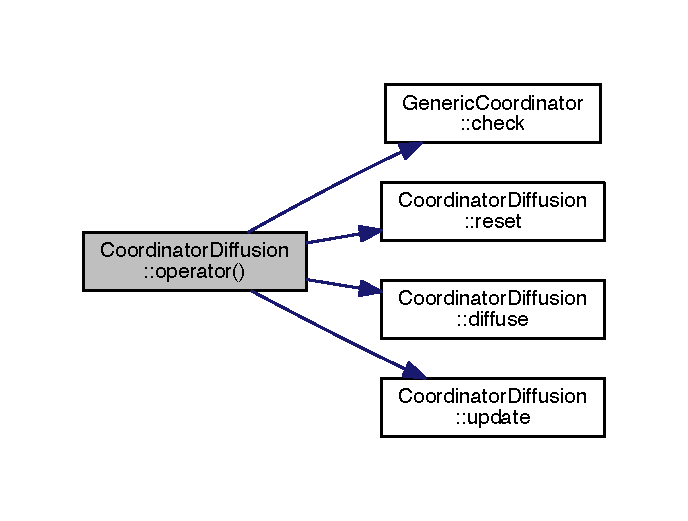
\includegraphics[width=330pt]{d3/dd2/class_coordinator_diffusion_a110e64039f79bcc6f0bfd430cb1f8c53_cgraph}
\end{center}
\end{figure}


\hypertarget{class_coordinator_diffusion_a496dde2de4c2ca2fe4d19dad33d2e93e}{}\index{Coordinator\+Diffusion@{Coordinator\+Diffusion}!reset@{reset}}
\index{reset@{reset}!Coordinator\+Diffusion@{Coordinator\+Diffusion}}
\subsubsection[{reset}]{\setlength{\rightskip}{0pt plus 5cm}template$<$typename Lab$>$ void {\bf Coordinator\+Diffusion}$<$ Lab $>$\+::reset (
\begin{DoxyParamCaption}
{}
\end{DoxyParamCaption}
)\hspace{0.3cm}{\ttfamily [inline]}, {\ttfamily [protected]}}\label{class_coordinator_diffusion_a496dde2de4c2ca2fe4d19dad33d2e93e}


Here is the caller graph for this function\+:\nopagebreak
\begin{figure}[H]
\begin{center}
\leavevmode
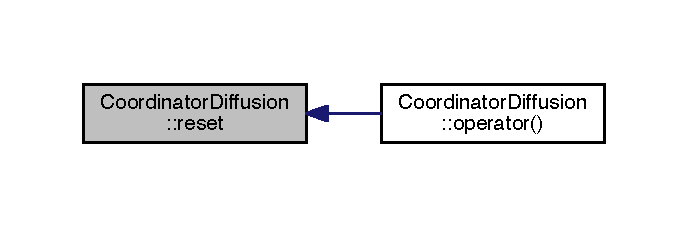
\includegraphics[width=330pt]{d3/dd2/class_coordinator_diffusion_a496dde2de4c2ca2fe4d19dad33d2e93e_icgraph}
\end{center}
\end{figure}


\hypertarget{class_coordinator_diffusion_aa3c7fd1a3955f9f5358e093b296992a0}{}\index{Coordinator\+Diffusion@{Coordinator\+Diffusion}!update@{update}}
\index{update@{update}!Coordinator\+Diffusion@{Coordinator\+Diffusion}}
\subsubsection[{update}]{\setlength{\rightskip}{0pt plus 5cm}template$<$typename Lab$>$ void {\bf Coordinator\+Diffusion}$<$ Lab $>$\+::update (
\begin{DoxyParamCaption}
{}
\end{DoxyParamCaption}
)\hspace{0.3cm}{\ttfamily [inline]}, {\ttfamily [protected]}}\label{class_coordinator_diffusion_aa3c7fd1a3955f9f5358e093b296992a0}


Here is the caller graph for this function\+:\nopagebreak
\begin{figure}[H]
\begin{center}
\leavevmode
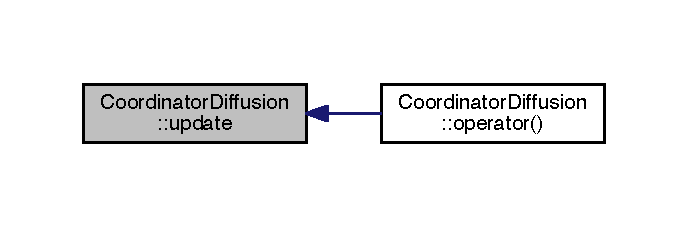
\includegraphics[width=330pt]{d3/dd2/class_coordinator_diffusion_aa3c7fd1a3955f9f5358e093b296992a0_icgraph}
\end{center}
\end{figure}




\subsection{Member Data Documentation}
\hypertarget{class_coordinator_diffusion_a8e1ee974d96ba320f26bcf7197e959fe}{}\index{Coordinator\+Diffusion@{Coordinator\+Diffusion}!coeff@{coeff}}
\index{coeff@{coeff}!Coordinator\+Diffusion@{Coordinator\+Diffusion}}
\subsubsection[{coeff}]{\setlength{\rightskip}{0pt plus 5cm}template$<$typename Lab$>$ const double {\bf Coordinator\+Diffusion}$<$ Lab $>$\+::coeff\hspace{0.3cm}{\ttfamily [protected]}}\label{class_coordinator_diffusion_a8e1ee974d96ba320f26bcf7197e959fe}


The documentation for this class was generated from the following file\+:\begin{DoxyCompactItemize}
\item 
/\+Users/cconti/\+Desktop/\+Mounts/\+Brutus\+Home/\+Cubism\+U\+P\+\_\+2\+D/source/\hyperlink{_coordinator_diffusion_8h}{Coordinator\+Diffusion.\+h}\end{DoxyCompactItemize}

\hypertarget{class_coordinator_gravity}{}\section{Coordinator\+Gravity Class Reference}
\label{class_coordinator_gravity}\index{Coordinator\+Gravity@{Coordinator\+Gravity}}


{\ttfamily \#include $<$Coordinator\+Gravity.\+h$>$}



Inheritance diagram for Coordinator\+Gravity\+:\nopagebreak
\begin{figure}[H]
\begin{center}
\leavevmode
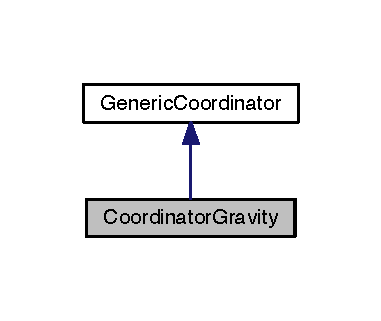
\includegraphics[width=183pt]{dc/dde/class_coordinator_gravity__inherit__graph}
\end{center}
\end{figure}


Collaboration diagram for Coordinator\+Gravity\+:\nopagebreak
\begin{figure}[H]
\begin{center}
\leavevmode
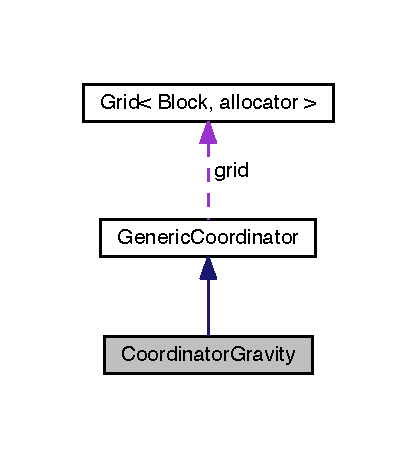
\includegraphics[width=200pt]{d4/d0d/class_coordinator_gravity__coll__graph}
\end{center}
\end{figure}
\subsection*{Public Member Functions}
\begin{DoxyCompactItemize}
\item 
\hyperlink{class_coordinator_gravity_aac9f22cb32fee8087ba202ad40cf129e}{Coordinator\+Gravity} (\hyperlink{_h_d_f5_dumper_8h_a445a5f0e2a34c9d97d69a3c2d1957907}{Real} \hyperlink{class_coordinator_gravity_a81013ceda5bc0f14b814569aaf5988a0}{gravity}\mbox{[}2\mbox{]}, \hyperlink{_definitions_8h_aff3288a3741f5098bcc456bb13440189}{Fluid\+Grid} $\ast$\hyperlink{class_generic_coordinator_aa514bbf7394bb5519c6f12daa33a375a}{grid})
\item 
void \hyperlink{class_coordinator_gravity_aa9066a9ec827fc22e02aa350c54b1198}{operator()} (const double dt)
\item 
\hyperlink{testfpzip_8cpp_a984bb8e04129c4268bd6ff36a50c9fa4}{string} \hyperlink{class_coordinator_gravity_ac58c205e291dfa7a9f703b7f10095ae2}{get\+Name} ()
\end{DoxyCompactItemize}
\subsection*{Protected Attributes}
\begin{DoxyCompactItemize}
\item 
\hyperlink{_h_d_f5_dumper_8h_a445a5f0e2a34c9d97d69a3c2d1957907}{Real} \hyperlink{class_coordinator_gravity_a81013ceda5bc0f14b814569aaf5988a0}{gravity} \mbox{[}2\mbox{]}
\end{DoxyCompactItemize}
\subsection*{Additional Inherited Members}


\subsection{Constructor \& Destructor Documentation}
\hypertarget{class_coordinator_gravity_aac9f22cb32fee8087ba202ad40cf129e}{}\index{Coordinator\+Gravity@{Coordinator\+Gravity}!Coordinator\+Gravity@{Coordinator\+Gravity}}
\index{Coordinator\+Gravity@{Coordinator\+Gravity}!Coordinator\+Gravity@{Coordinator\+Gravity}}
\subsubsection[{Coordinator\+Gravity}]{\setlength{\rightskip}{0pt plus 5cm}Coordinator\+Gravity\+::\+Coordinator\+Gravity (
\begin{DoxyParamCaption}
\item[{{\bf Real}}]{gravity\mbox{[}2\mbox{]}, }
\item[{{\bf Fluid\+Grid} $\ast$}]{grid}
\end{DoxyParamCaption}
)\hspace{0.3cm}{\ttfamily [inline]}}\label{class_coordinator_gravity_aac9f22cb32fee8087ba202ad40cf129e}


\subsection{Member Function Documentation}
\hypertarget{class_coordinator_gravity_ac58c205e291dfa7a9f703b7f10095ae2}{}\index{Coordinator\+Gravity@{Coordinator\+Gravity}!get\+Name@{get\+Name}}
\index{get\+Name@{get\+Name}!Coordinator\+Gravity@{Coordinator\+Gravity}}
\subsubsection[{get\+Name}]{\setlength{\rightskip}{0pt plus 5cm}{\bf string} Coordinator\+Gravity\+::get\+Name (
\begin{DoxyParamCaption}
{}
\end{DoxyParamCaption}
)\hspace{0.3cm}{\ttfamily [inline]}, {\ttfamily [virtual]}}\label{class_coordinator_gravity_ac58c205e291dfa7a9f703b7f10095ae2}


Implements \hyperlink{class_generic_coordinator_a8c1b9f4fa96d1c7b851e85e19325de1d}{Generic\+Coordinator}.

\hypertarget{class_coordinator_gravity_aa9066a9ec827fc22e02aa350c54b1198}{}\index{Coordinator\+Gravity@{Coordinator\+Gravity}!operator()@{operator()}}
\index{operator()@{operator()}!Coordinator\+Gravity@{Coordinator\+Gravity}}
\subsubsection[{operator()}]{\setlength{\rightskip}{0pt plus 5cm}void Coordinator\+Gravity\+::operator() (
\begin{DoxyParamCaption}
\item[{const double}]{dt}
\end{DoxyParamCaption}
)\hspace{0.3cm}{\ttfamily [inline]}, {\ttfamily [virtual]}}\label{class_coordinator_gravity_aa9066a9ec827fc22e02aa350c54b1198}


Implements \hyperlink{class_generic_coordinator_a984696fef63daf7253b87ce21cce3f94}{Generic\+Coordinator}.



Here is the call graph for this function\+:\nopagebreak
\begin{figure}[H]
\begin{center}
\leavevmode
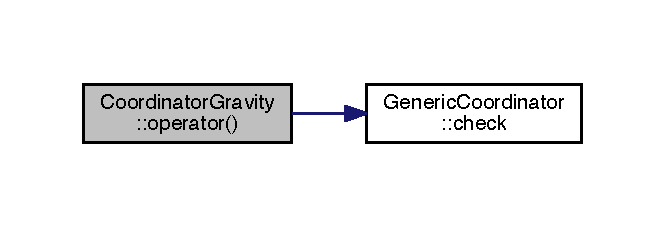
\includegraphics[width=319pt]{dd/dd9/class_coordinator_gravity_aa9066a9ec827fc22e02aa350c54b1198_cgraph}
\end{center}
\end{figure}




\subsection{Member Data Documentation}
\hypertarget{class_coordinator_gravity_a81013ceda5bc0f14b814569aaf5988a0}{}\index{Coordinator\+Gravity@{Coordinator\+Gravity}!gravity@{gravity}}
\index{gravity@{gravity}!Coordinator\+Gravity@{Coordinator\+Gravity}}
\subsubsection[{gravity}]{\setlength{\rightskip}{0pt plus 5cm}{\bf Real} Coordinator\+Gravity\+::gravity\mbox{[}2\mbox{]}\hspace{0.3cm}{\ttfamily [protected]}}\label{class_coordinator_gravity_a81013ceda5bc0f14b814569aaf5988a0}


The documentation for this class was generated from the following file\+:\begin{DoxyCompactItemize}
\item 
/\+Users/cconti/\+Desktop/\+Mounts/\+Brutus\+Home/\+Cubism\+U\+P\+\_\+2\+D/source/\hyperlink{_coordinator_gravity_8h}{Coordinator\+Gravity.\+h}\end{DoxyCompactItemize}

\hypertarget{class_coordinator_i_c}{}\section{Coordinator\+I\+C Class Reference}
\label{class_coordinator_i_c}\index{Coordinator\+I\+C@{Coordinator\+I\+C}}


{\ttfamily \#include $<$Coordinator\+I\+C.\+h$>$}



Inheritance diagram for Coordinator\+I\+C\+:\nopagebreak
\begin{figure}[H]
\begin{center}
\leavevmode
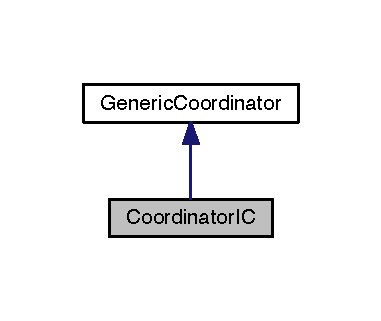
\includegraphics[width=183pt]{db/d5e/class_coordinator_i_c__inherit__graph}
\end{center}
\end{figure}


Collaboration diagram for Coordinator\+I\+C\+:\nopagebreak
\begin{figure}[H]
\begin{center}
\leavevmode
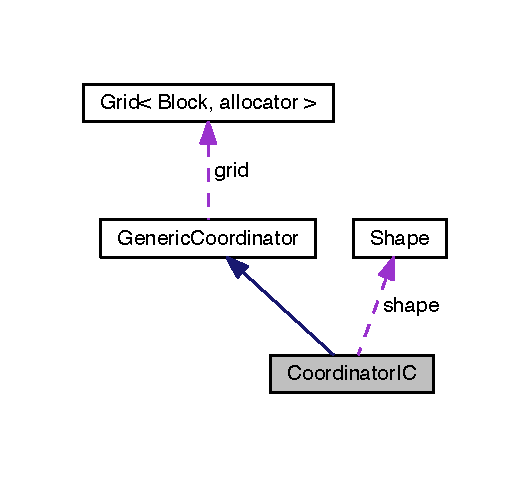
\includegraphics[width=254pt]{df/dc1/class_coordinator_i_c__coll__graph}
\end{center}
\end{figure}
\subsection*{Public Member Functions}
\begin{DoxyCompactItemize}
\item 
\hyperlink{class_coordinator_i_c_ae2785fbb83c0f06da7d5337245d0a73b}{Coordinator\+I\+C} (\hyperlink{class_shape}{Shape} $\ast$\hyperlink{class_coordinator_i_c_ad8c925b22185d579c2cf734d597422f0}{shape}, const double \hyperlink{class_coordinator_i_c_aa5b9d4280795a2dc60e9008ced9811fe}{uinf}, \hyperlink{_definitions_8h_aff3288a3741f5098bcc456bb13440189}{Fluid\+Grid} $\ast$\hyperlink{class_generic_coordinator_aa514bbf7394bb5519c6f12daa33a375a}{grid})
\item 
void \hyperlink{class_coordinator_i_c_a75f8e04638d34d0a726f0e1b0939be1e}{operator()} (const double dt)
\item 
\hyperlink{testfpzip_8cpp_a984bb8e04129c4268bd6ff36a50c9fa4}{string} \hyperlink{class_coordinator_i_c_a1c90cddb95853cb32253c56db4661633}{get\+Name} ()
\end{DoxyCompactItemize}
\subsection*{Protected Attributes}
\begin{DoxyCompactItemize}
\item 
\hyperlink{class_shape}{Shape} $\ast$ \hyperlink{class_coordinator_i_c_ad8c925b22185d579c2cf734d597422f0}{shape}
\item 
const double \hyperlink{class_coordinator_i_c_aa5b9d4280795a2dc60e9008ced9811fe}{uinf}
\end{DoxyCompactItemize}
\subsection*{Additional Inherited Members}


\subsection{Constructor \& Destructor Documentation}
\hypertarget{class_coordinator_i_c_ae2785fbb83c0f06da7d5337245d0a73b}{}\index{Coordinator\+I\+C@{Coordinator\+I\+C}!Coordinator\+I\+C@{Coordinator\+I\+C}}
\index{Coordinator\+I\+C@{Coordinator\+I\+C}!Coordinator\+I\+C@{Coordinator\+I\+C}}
\subsubsection[{Coordinator\+I\+C}]{\setlength{\rightskip}{0pt plus 5cm}Coordinator\+I\+C\+::\+Coordinator\+I\+C (
\begin{DoxyParamCaption}
\item[{{\bf Shape} $\ast$}]{shape, }
\item[{const double}]{uinf, }
\item[{{\bf Fluid\+Grid} $\ast$}]{grid}
\end{DoxyParamCaption}
)\hspace{0.3cm}{\ttfamily [inline]}}\label{class_coordinator_i_c_ae2785fbb83c0f06da7d5337245d0a73b}


\subsection{Member Function Documentation}
\hypertarget{class_coordinator_i_c_a1c90cddb95853cb32253c56db4661633}{}\index{Coordinator\+I\+C@{Coordinator\+I\+C}!get\+Name@{get\+Name}}
\index{get\+Name@{get\+Name}!Coordinator\+I\+C@{Coordinator\+I\+C}}
\subsubsection[{get\+Name}]{\setlength{\rightskip}{0pt plus 5cm}{\bf string} Coordinator\+I\+C\+::get\+Name (
\begin{DoxyParamCaption}
{}
\end{DoxyParamCaption}
)\hspace{0.3cm}{\ttfamily [inline]}, {\ttfamily [virtual]}}\label{class_coordinator_i_c_a1c90cddb95853cb32253c56db4661633}


Implements \hyperlink{class_generic_coordinator_a8c1b9f4fa96d1c7b851e85e19325de1d}{Generic\+Coordinator}.



Here is the caller graph for this function\+:\nopagebreak
\begin{figure}[H]
\begin{center}
\leavevmode
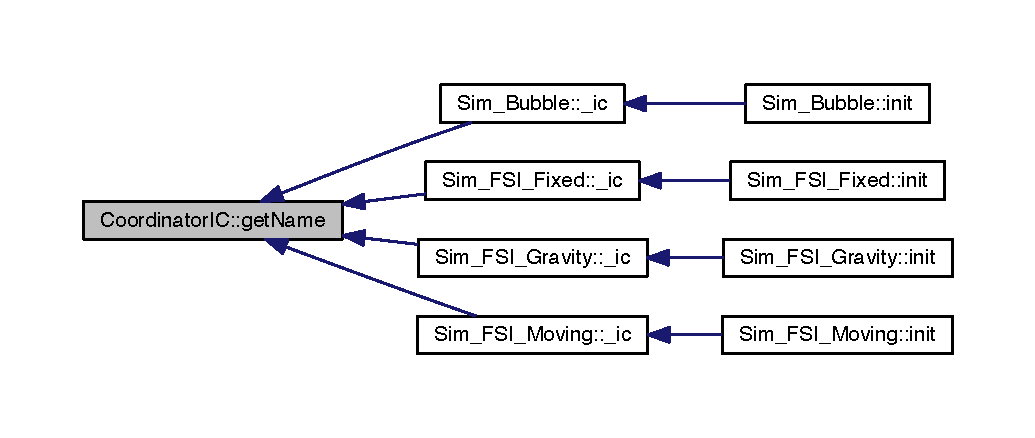
\includegraphics[width=350pt]{da/dd2/class_coordinator_i_c_a1c90cddb95853cb32253c56db4661633_icgraph}
\end{center}
\end{figure}


\hypertarget{class_coordinator_i_c_a75f8e04638d34d0a726f0e1b0939be1e}{}\index{Coordinator\+I\+C@{Coordinator\+I\+C}!operator()@{operator()}}
\index{operator()@{operator()}!Coordinator\+I\+C@{Coordinator\+I\+C}}
\subsubsection[{operator()}]{\setlength{\rightskip}{0pt plus 5cm}void Coordinator\+I\+C\+::operator() (
\begin{DoxyParamCaption}
\item[{const double}]{dt}
\end{DoxyParamCaption}
)\hspace{0.3cm}{\ttfamily [inline]}, {\ttfamily [virtual]}}\label{class_coordinator_i_c_a75f8e04638d34d0a726f0e1b0939be1e}


Implements \hyperlink{class_generic_coordinator_a984696fef63daf7253b87ce21cce3f94}{Generic\+Coordinator}.



Here is the call graph for this function\+:\nopagebreak
\begin{figure}[H]
\begin{center}
\leavevmode
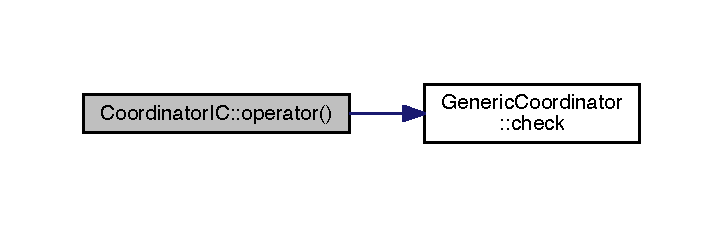
\includegraphics[width=347pt]{da/dd2/class_coordinator_i_c_a75f8e04638d34d0a726f0e1b0939be1e_cgraph}
\end{center}
\end{figure}




\subsection{Member Data Documentation}
\hypertarget{class_coordinator_i_c_ad8c925b22185d579c2cf734d597422f0}{}\index{Coordinator\+I\+C@{Coordinator\+I\+C}!shape@{shape}}
\index{shape@{shape}!Coordinator\+I\+C@{Coordinator\+I\+C}}
\subsubsection[{shape}]{\setlength{\rightskip}{0pt plus 5cm}{\bf Shape}$\ast$ Coordinator\+I\+C\+::shape\hspace{0.3cm}{\ttfamily [protected]}}\label{class_coordinator_i_c_ad8c925b22185d579c2cf734d597422f0}
\hypertarget{class_coordinator_i_c_aa5b9d4280795a2dc60e9008ced9811fe}{}\index{Coordinator\+I\+C@{Coordinator\+I\+C}!uinf@{uinf}}
\index{uinf@{uinf}!Coordinator\+I\+C@{Coordinator\+I\+C}}
\subsubsection[{uinf}]{\setlength{\rightskip}{0pt plus 5cm}const double Coordinator\+I\+C\+::uinf\hspace{0.3cm}{\ttfamily [protected]}}\label{class_coordinator_i_c_aa5b9d4280795a2dc60e9008ced9811fe}


The documentation for this class was generated from the following file\+:\begin{DoxyCompactItemize}
\item 
/\+Users/cconti/\+Desktop/\+Mounts/\+Brutus\+Home/\+Cubism\+U\+P\+\_\+2\+D/source/\hyperlink{_coordinator_i_c_8h}{Coordinator\+I\+C.\+h}\end{DoxyCompactItemize}

\hypertarget{class_coordinator_i_c___r_t}{}\section{Coordinator\+I\+C\+\_\+\+R\+T Class Reference}
\label{class_coordinator_i_c___r_t}\index{Coordinator\+I\+C\+\_\+\+R\+T@{Coordinator\+I\+C\+\_\+\+R\+T}}


{\ttfamily \#include $<$Coordinator\+I\+C.\+h$>$}



Inheritance diagram for Coordinator\+I\+C\+\_\+\+R\+T\+:\nopagebreak
\begin{figure}[H]
\begin{center}
\leavevmode
\includegraphics[width=183pt]{d2/d60/class_coordinator_i_c___r_t__inherit__graph}
\end{center}
\end{figure}


Collaboration diagram for Coordinator\+I\+C\+\_\+\+R\+T\+:\nopagebreak
\begin{figure}[H]
\begin{center}
\leavevmode
\includegraphics[width=200pt]{d9/d6d/class_coordinator_i_c___r_t__coll__graph}
\end{center}
\end{figure}
\subsection*{Public Member Functions}
\begin{DoxyCompactItemize}
\item 
\hyperlink{class_coordinator_i_c___r_t_a93384b52957c59a997c364ea8cafbd1d}{Coordinator\+I\+C\+\_\+\+R\+T} (const double \hyperlink{class_coordinator_i_c___r_t_abb42cd766cee753162f3c01009b72058}{rho\+S}, \hyperlink{_definitions_8h_aff3288a3741f5098bcc456bb13440189}{Fluid\+Grid} $\ast$\hyperlink{class_generic_coordinator_aa514bbf7394bb5519c6f12daa33a375a}{grid})
\item 
void \hyperlink{class_coordinator_i_c___r_t_a4a8653482a770c346ff8939a2f92a4af}{operator()} (const double dt)
\item 
\hyperlink{testfpzip_8cpp_a984bb8e04129c4268bd6ff36a50c9fa4}{string} \hyperlink{class_coordinator_i_c___r_t_ad0d84043cb7d82f799f5cddff520e2c7}{get\+Name} ()
\end{DoxyCompactItemize}
\subsection*{Protected Attributes}
\begin{DoxyCompactItemize}
\item 
const double \hyperlink{class_coordinator_i_c___r_t_abb42cd766cee753162f3c01009b72058}{rho\+S}
\end{DoxyCompactItemize}
\subsection*{Additional Inherited Members}


\subsection{Constructor \& Destructor Documentation}
\hypertarget{class_coordinator_i_c___r_t_a93384b52957c59a997c364ea8cafbd1d}{}\index{Coordinator\+I\+C\+\_\+\+R\+T@{Coordinator\+I\+C\+\_\+\+R\+T}!Coordinator\+I\+C\+\_\+\+R\+T@{Coordinator\+I\+C\+\_\+\+R\+T}}
\index{Coordinator\+I\+C\+\_\+\+R\+T@{Coordinator\+I\+C\+\_\+\+R\+T}!Coordinator\+I\+C\+\_\+\+R\+T@{Coordinator\+I\+C\+\_\+\+R\+T}}
\subsubsection[{Coordinator\+I\+C\+\_\+\+R\+T}]{\setlength{\rightskip}{0pt plus 5cm}Coordinator\+I\+C\+\_\+\+R\+T\+::\+Coordinator\+I\+C\+\_\+\+R\+T (
\begin{DoxyParamCaption}
\item[{const double}]{rho\+S, }
\item[{{\bf Fluid\+Grid} $\ast$}]{grid}
\end{DoxyParamCaption}
)\hspace{0.3cm}{\ttfamily [inline]}}\label{class_coordinator_i_c___r_t_a93384b52957c59a997c364ea8cafbd1d}


\subsection{Member Function Documentation}
\hypertarget{class_coordinator_i_c___r_t_ad0d84043cb7d82f799f5cddff520e2c7}{}\index{Coordinator\+I\+C\+\_\+\+R\+T@{Coordinator\+I\+C\+\_\+\+R\+T}!get\+Name@{get\+Name}}
\index{get\+Name@{get\+Name}!Coordinator\+I\+C\+\_\+\+R\+T@{Coordinator\+I\+C\+\_\+\+R\+T}}
\subsubsection[{get\+Name}]{\setlength{\rightskip}{0pt plus 5cm}{\bf string} Coordinator\+I\+C\+\_\+\+R\+T\+::get\+Name (
\begin{DoxyParamCaption}
{}
\end{DoxyParamCaption}
)\hspace{0.3cm}{\ttfamily [inline]}, {\ttfamily [virtual]}}\label{class_coordinator_i_c___r_t_ad0d84043cb7d82f799f5cddff520e2c7}


Implements \hyperlink{class_generic_coordinator_a8c1b9f4fa96d1c7b851e85e19325de1d}{Generic\+Coordinator}.



Here is the caller graph for this function\+:\nopagebreak
\begin{figure}[H]
\begin{center}
\leavevmode
\includegraphics[width=350pt]{de/d5f/class_coordinator_i_c___r_t_ad0d84043cb7d82f799f5cddff520e2c7_icgraph}
\end{center}
\end{figure}


\hypertarget{class_coordinator_i_c___r_t_a4a8653482a770c346ff8939a2f92a4af}{}\index{Coordinator\+I\+C\+\_\+\+R\+T@{Coordinator\+I\+C\+\_\+\+R\+T}!operator()@{operator()}}
\index{operator()@{operator()}!Coordinator\+I\+C\+\_\+\+R\+T@{Coordinator\+I\+C\+\_\+\+R\+T}}
\subsubsection[{operator()}]{\setlength{\rightskip}{0pt plus 5cm}void Coordinator\+I\+C\+\_\+\+R\+T\+::operator() (
\begin{DoxyParamCaption}
\item[{const double}]{dt}
\end{DoxyParamCaption}
)\hspace{0.3cm}{\ttfamily [inline]}, {\ttfamily [virtual]}}\label{class_coordinator_i_c___r_t_a4a8653482a770c346ff8939a2f92a4af}


Implements \hyperlink{class_generic_coordinator_a984696fef63daf7253b87ce21cce3f94}{Generic\+Coordinator}.



Here is the call graph for this function\+:\nopagebreak
\begin{figure}[H]
\begin{center}
\leavevmode
\includegraphics[width=350pt]{de/d5f/class_coordinator_i_c___r_t_a4a8653482a770c346ff8939a2f92a4af_cgraph}
\end{center}
\end{figure}




\subsection{Member Data Documentation}
\hypertarget{class_coordinator_i_c___r_t_abb42cd766cee753162f3c01009b72058}{}\index{Coordinator\+I\+C\+\_\+\+R\+T@{Coordinator\+I\+C\+\_\+\+R\+T}!rho\+S@{rho\+S}}
\index{rho\+S@{rho\+S}!Coordinator\+I\+C\+\_\+\+R\+T@{Coordinator\+I\+C\+\_\+\+R\+T}}
\subsubsection[{rho\+S}]{\setlength{\rightskip}{0pt plus 5cm}const double Coordinator\+I\+C\+\_\+\+R\+T\+::rho\+S\hspace{0.3cm}{\ttfamily [protected]}}\label{class_coordinator_i_c___r_t_abb42cd766cee753162f3c01009b72058}


The documentation for this class was generated from the following file\+:\begin{DoxyCompactItemize}
\item 
/\+Users/cconti/\+Desktop/\+Mounts/\+Brutus\+Home/\+Cubism\+U\+P\+\_\+2\+D/source/\hyperlink{_coordinator_i_c_8h}{Coordinator\+I\+C.\+h}\end{DoxyCompactItemize}

\hypertarget{class_coordinator_penalization}{}\section{Coordinator\+Penalization Class Reference}
\label{class_coordinator_penalization}\index{Coordinator\+Penalization@{Coordinator\+Penalization}}


{\ttfamily \#include $<$Coordinator\+Penalization.\+h$>$}



Inheritance diagram for Coordinator\+Penalization\+:\nopagebreak
\begin{figure}[H]
\begin{center}
\leavevmode
\includegraphics[width=203pt]{d9/d00/class_coordinator_penalization__inherit__graph}
\end{center}
\end{figure}


Collaboration diagram for Coordinator\+Penalization\+:\nopagebreak
\begin{figure}[H]
\begin{center}
\leavevmode
\includegraphics[width=270pt]{dd/d9f/class_coordinator_penalization__coll__graph}
\end{center}
\end{figure}
\subsection*{Public Member Functions}
\begin{DoxyCompactItemize}
\item 
\hyperlink{class_coordinator_penalization_a6f84806707709981c60711eb56f9cac2}{Coordinator\+Penalization} (\hyperlink{_h_d_f5_dumper_8h_a445a5f0e2a34c9d97d69a3c2d1957907}{Real} $\ast$\hyperlink{class_coordinator_penalization_a69c4aa62739ebf73ddba8c688c4212d7}{u\+Body}, \hyperlink{_h_d_f5_dumper_8h_a445a5f0e2a34c9d97d69a3c2d1957907}{Real} $\ast$\hyperlink{class_coordinator_penalization_a0e387ed3e8f65a876de9e44dcd866c58}{v\+Body}, \hyperlink{_h_d_f5_dumper_8h_a445a5f0e2a34c9d97d69a3c2d1957907}{Real} $\ast$\hyperlink{class_coordinator_penalization_af18f7de3308e47cdd39a367f843276f0}{omega\+Body}, \hyperlink{class_shape}{Shape} $\ast$\hyperlink{class_coordinator_penalization_a1d686d4837782669fe4048d8247694e4}{shape}, \hyperlink{_h_d_f5_dumper_8h_a445a5f0e2a34c9d97d69a3c2d1957907}{Real} \hyperlink{class_coordinator_penalization_a1fb2d57c01272130fcc1db62b6e61db3}{lambda}, \hyperlink{_definitions_8h_aff3288a3741f5098bcc456bb13440189}{Fluid\+Grid} $\ast$\hyperlink{class_generic_coordinator_aa514bbf7394bb5519c6f12daa33a375a}{grid})
\item 
void \hyperlink{class_coordinator_penalization_ac6138327b1de95c0cf53d0ed47872292}{operator()} (const double dt)
\item 
\hyperlink{testfpzip_8cpp_a984bb8e04129c4268bd6ff36a50c9fa4}{string} \hyperlink{class_coordinator_penalization_ae53f97c939755a01f3eba9c20a78f2e4}{get\+Name} ()
\end{DoxyCompactItemize}
\subsection*{Protected Attributes}
\begin{DoxyCompactItemize}
\item 
\hyperlink{_h_d_f5_dumper_8h_a445a5f0e2a34c9d97d69a3c2d1957907}{Real} $\ast$ \hyperlink{class_coordinator_penalization_a69c4aa62739ebf73ddba8c688c4212d7}{u\+Body}
\item 
\hyperlink{_h_d_f5_dumper_8h_a445a5f0e2a34c9d97d69a3c2d1957907}{Real} $\ast$ \hyperlink{class_coordinator_penalization_a0e387ed3e8f65a876de9e44dcd866c58}{v\+Body}
\item 
\hyperlink{_h_d_f5_dumper_8h_a445a5f0e2a34c9d97d69a3c2d1957907}{Real} $\ast$ \hyperlink{class_coordinator_penalization_af18f7de3308e47cdd39a367f843276f0}{omega\+Body}
\item 
\hyperlink{class_shape}{Shape} $\ast$ \hyperlink{class_coordinator_penalization_a1d686d4837782669fe4048d8247694e4}{shape}
\item 
\hyperlink{_h_d_f5_dumper_8h_a445a5f0e2a34c9d97d69a3c2d1957907}{Real} \hyperlink{class_coordinator_penalization_a1fb2d57c01272130fcc1db62b6e61db3}{lambda}
\end{DoxyCompactItemize}
\subsection*{Additional Inherited Members}


\subsection{Constructor \& Destructor Documentation}
\hypertarget{class_coordinator_penalization_a6f84806707709981c60711eb56f9cac2}{}\index{Coordinator\+Penalization@{Coordinator\+Penalization}!Coordinator\+Penalization@{Coordinator\+Penalization}}
\index{Coordinator\+Penalization@{Coordinator\+Penalization}!Coordinator\+Penalization@{Coordinator\+Penalization}}
\subsubsection[{Coordinator\+Penalization}]{\setlength{\rightskip}{0pt plus 5cm}Coordinator\+Penalization\+::\+Coordinator\+Penalization (
\begin{DoxyParamCaption}
\item[{{\bf Real} $\ast$}]{u\+Body, }
\item[{{\bf Real} $\ast$}]{v\+Body, }
\item[{{\bf Real} $\ast$}]{omega\+Body, }
\item[{{\bf Shape} $\ast$}]{shape, }
\item[{{\bf Real}}]{lambda, }
\item[{{\bf Fluid\+Grid} $\ast$}]{grid}
\end{DoxyParamCaption}
)\hspace{0.3cm}{\ttfamily [inline]}}\label{class_coordinator_penalization_a6f84806707709981c60711eb56f9cac2}


\subsection{Member Function Documentation}
\hypertarget{class_coordinator_penalization_ae53f97c939755a01f3eba9c20a78f2e4}{}\index{Coordinator\+Penalization@{Coordinator\+Penalization}!get\+Name@{get\+Name}}
\index{get\+Name@{get\+Name}!Coordinator\+Penalization@{Coordinator\+Penalization}}
\subsubsection[{get\+Name}]{\setlength{\rightskip}{0pt plus 5cm}{\bf string} Coordinator\+Penalization\+::get\+Name (
\begin{DoxyParamCaption}
{}
\end{DoxyParamCaption}
)\hspace{0.3cm}{\ttfamily [inline]}, {\ttfamily [virtual]}}\label{class_coordinator_penalization_ae53f97c939755a01f3eba9c20a78f2e4}


Implements \hyperlink{class_generic_coordinator_a8c1b9f4fa96d1c7b851e85e19325de1d}{Generic\+Coordinator}.

\hypertarget{class_coordinator_penalization_ac6138327b1de95c0cf53d0ed47872292}{}\index{Coordinator\+Penalization@{Coordinator\+Penalization}!operator()@{operator()}}
\index{operator()@{operator()}!Coordinator\+Penalization@{Coordinator\+Penalization}}
\subsubsection[{operator()}]{\setlength{\rightskip}{0pt plus 5cm}void Coordinator\+Penalization\+::operator() (
\begin{DoxyParamCaption}
\item[{const double}]{dt}
\end{DoxyParamCaption}
)\hspace{0.3cm}{\ttfamily [inline]}, {\ttfamily [virtual]}}\label{class_coordinator_penalization_ac6138327b1de95c0cf53d0ed47872292}


Implements \hyperlink{class_generic_coordinator_a984696fef63daf7253b87ce21cce3f94}{Generic\+Coordinator}.



Here is the call graph for this function\+:\nopagebreak
\begin{figure}[H]
\begin{center}
\leavevmode
\includegraphics[width=342pt]{d3/d93/class_coordinator_penalization_ac6138327b1de95c0cf53d0ed47872292_cgraph}
\end{center}
\end{figure}




\subsection{Member Data Documentation}
\hypertarget{class_coordinator_penalization_a1fb2d57c01272130fcc1db62b6e61db3}{}\index{Coordinator\+Penalization@{Coordinator\+Penalization}!lambda@{lambda}}
\index{lambda@{lambda}!Coordinator\+Penalization@{Coordinator\+Penalization}}
\subsubsection[{lambda}]{\setlength{\rightskip}{0pt plus 5cm}{\bf Real} Coordinator\+Penalization\+::lambda\hspace{0.3cm}{\ttfamily [protected]}}\label{class_coordinator_penalization_a1fb2d57c01272130fcc1db62b6e61db3}
\hypertarget{class_coordinator_penalization_af18f7de3308e47cdd39a367f843276f0}{}\index{Coordinator\+Penalization@{Coordinator\+Penalization}!omega\+Body@{omega\+Body}}
\index{omega\+Body@{omega\+Body}!Coordinator\+Penalization@{Coordinator\+Penalization}}
\subsubsection[{omega\+Body}]{\setlength{\rightskip}{0pt plus 5cm}{\bf Real} $\ast$ Coordinator\+Penalization\+::omega\+Body\hspace{0.3cm}{\ttfamily [protected]}}\label{class_coordinator_penalization_af18f7de3308e47cdd39a367f843276f0}
\hypertarget{class_coordinator_penalization_a1d686d4837782669fe4048d8247694e4}{}\index{Coordinator\+Penalization@{Coordinator\+Penalization}!shape@{shape}}
\index{shape@{shape}!Coordinator\+Penalization@{Coordinator\+Penalization}}
\subsubsection[{shape}]{\setlength{\rightskip}{0pt plus 5cm}{\bf Shape}$\ast$ Coordinator\+Penalization\+::shape\hspace{0.3cm}{\ttfamily [protected]}}\label{class_coordinator_penalization_a1d686d4837782669fe4048d8247694e4}
\hypertarget{class_coordinator_penalization_a69c4aa62739ebf73ddba8c688c4212d7}{}\index{Coordinator\+Penalization@{Coordinator\+Penalization}!u\+Body@{u\+Body}}
\index{u\+Body@{u\+Body}!Coordinator\+Penalization@{Coordinator\+Penalization}}
\subsubsection[{u\+Body}]{\setlength{\rightskip}{0pt plus 5cm}{\bf Real}$\ast$ Coordinator\+Penalization\+::u\+Body\hspace{0.3cm}{\ttfamily [protected]}}\label{class_coordinator_penalization_a69c4aa62739ebf73ddba8c688c4212d7}
\hypertarget{class_coordinator_penalization_a0e387ed3e8f65a876de9e44dcd866c58}{}\index{Coordinator\+Penalization@{Coordinator\+Penalization}!v\+Body@{v\+Body}}
\index{v\+Body@{v\+Body}!Coordinator\+Penalization@{Coordinator\+Penalization}}
\subsubsection[{v\+Body}]{\setlength{\rightskip}{0pt plus 5cm}{\bf Real} $\ast$ Coordinator\+Penalization\+::v\+Body\hspace{0.3cm}{\ttfamily [protected]}}\label{class_coordinator_penalization_a0e387ed3e8f65a876de9e44dcd866c58}


The documentation for this class was generated from the following file\+:\begin{DoxyCompactItemize}
\item 
/\+Users/cconti/\+Desktop/\+Mounts/\+Brutus\+Home/\+Cubism\+U\+P\+\_\+2\+D/source/\hyperlink{_coordinator_penalization_8h}{Coordinator\+Penalization.\+h}\end{DoxyCompactItemize}

\hypertarget{class_coordinator_penalization_fixed}{}\section{Coordinator\+Penalization\+Fixed Class Reference}
\label{class_coordinator_penalization_fixed}\index{Coordinator\+Penalization\+Fixed@{Coordinator\+Penalization\+Fixed}}


{\ttfamily \#include $<$Coordinator\+Penalization.\+h$>$}



Inheritance diagram for Coordinator\+Penalization\+Fixed\+:\nopagebreak
\begin{figure}[H]
\begin{center}
\leavevmode
\includegraphics[width=227pt]{df/d9b/class_coordinator_penalization_fixed__inherit__graph}
\end{center}
\end{figure}


Collaboration diagram for Coordinator\+Penalization\+Fixed\+:\nopagebreak
\begin{figure}[H]
\begin{center}
\leavevmode
\includegraphics[width=283pt]{d4/d66/class_coordinator_penalization_fixed__coll__graph}
\end{center}
\end{figure}
\subsection*{Public Member Functions}
\begin{DoxyCompactItemize}
\item 
\hyperlink{class_coordinator_penalization_fixed_abc95008ee4fa6d71b19c590853e68ec8}{Coordinator\+Penalization\+Fixed} (\hyperlink{class_shape}{Shape} $\ast$\hyperlink{class_coordinator_penalization_fixed_a548e655ec26679bdb0f1c2d12f039f1f}{shape}, \hyperlink{_h_d_f5_dumper_8h_a445a5f0e2a34c9d97d69a3c2d1957907}{Real} \hyperlink{class_coordinator_penalization_fixed_a5e9ee0336487fa3980dbad77f51c50ba}{lambda}, \hyperlink{_definitions_8h_aff3288a3741f5098bcc456bb13440189}{Fluid\+Grid} $\ast$\hyperlink{class_generic_coordinator_aa514bbf7394bb5519c6f12daa33a375a}{grid})
\item 
void \hyperlink{class_coordinator_penalization_fixed_adb344c7e7ded7b7e8f4d948c38d0c980}{operator()} (const double dt)
\item 
\hyperlink{testfpzip_8cpp_a984bb8e04129c4268bd6ff36a50c9fa4}{string} \hyperlink{class_coordinator_penalization_fixed_a6dcdebd82a4cbc37ce47806d5f8cfa93}{get\+Name} ()
\end{DoxyCompactItemize}
\subsection*{Protected Attributes}
\begin{DoxyCompactItemize}
\item 
\hyperlink{class_shape}{Shape} $\ast$ \hyperlink{class_coordinator_penalization_fixed_a548e655ec26679bdb0f1c2d12f039f1f}{shape}
\item 
\hyperlink{_h_d_f5_dumper_8h_a445a5f0e2a34c9d97d69a3c2d1957907}{Real} \hyperlink{class_coordinator_penalization_fixed_a5e9ee0336487fa3980dbad77f51c50ba}{lambda}
\end{DoxyCompactItemize}
\subsection*{Additional Inherited Members}


\subsection{Constructor \& Destructor Documentation}
\hypertarget{class_coordinator_penalization_fixed_abc95008ee4fa6d71b19c590853e68ec8}{}\index{Coordinator\+Penalization\+Fixed@{Coordinator\+Penalization\+Fixed}!Coordinator\+Penalization\+Fixed@{Coordinator\+Penalization\+Fixed}}
\index{Coordinator\+Penalization\+Fixed@{Coordinator\+Penalization\+Fixed}!Coordinator\+Penalization\+Fixed@{Coordinator\+Penalization\+Fixed}}
\subsubsection[{Coordinator\+Penalization\+Fixed}]{\setlength{\rightskip}{0pt plus 5cm}Coordinator\+Penalization\+Fixed\+::\+Coordinator\+Penalization\+Fixed (
\begin{DoxyParamCaption}
\item[{{\bf Shape} $\ast$}]{shape, }
\item[{{\bf Real}}]{lambda, }
\item[{{\bf Fluid\+Grid} $\ast$}]{grid}
\end{DoxyParamCaption}
)\hspace{0.3cm}{\ttfamily [inline]}}\label{class_coordinator_penalization_fixed_abc95008ee4fa6d71b19c590853e68ec8}


\subsection{Member Function Documentation}
\hypertarget{class_coordinator_penalization_fixed_a6dcdebd82a4cbc37ce47806d5f8cfa93}{}\index{Coordinator\+Penalization\+Fixed@{Coordinator\+Penalization\+Fixed}!get\+Name@{get\+Name}}
\index{get\+Name@{get\+Name}!Coordinator\+Penalization\+Fixed@{Coordinator\+Penalization\+Fixed}}
\subsubsection[{get\+Name}]{\setlength{\rightskip}{0pt plus 5cm}{\bf string} Coordinator\+Penalization\+Fixed\+::get\+Name (
\begin{DoxyParamCaption}
{}
\end{DoxyParamCaption}
)\hspace{0.3cm}{\ttfamily [inline]}, {\ttfamily [virtual]}}\label{class_coordinator_penalization_fixed_a6dcdebd82a4cbc37ce47806d5f8cfa93}


Implements \hyperlink{class_generic_coordinator_a8c1b9f4fa96d1c7b851e85e19325de1d}{Generic\+Coordinator}.

\hypertarget{class_coordinator_penalization_fixed_adb344c7e7ded7b7e8f4d948c38d0c980}{}\index{Coordinator\+Penalization\+Fixed@{Coordinator\+Penalization\+Fixed}!operator()@{operator()}}
\index{operator()@{operator()}!Coordinator\+Penalization\+Fixed@{Coordinator\+Penalization\+Fixed}}
\subsubsection[{operator()}]{\setlength{\rightskip}{0pt plus 5cm}void Coordinator\+Penalization\+Fixed\+::operator() (
\begin{DoxyParamCaption}
\item[{const double}]{dt}
\end{DoxyParamCaption}
)\hspace{0.3cm}{\ttfamily [inline]}, {\ttfamily [virtual]}}\label{class_coordinator_penalization_fixed_adb344c7e7ded7b7e8f4d948c38d0c980}


Implements \hyperlink{class_generic_coordinator_a984696fef63daf7253b87ce21cce3f94}{Generic\+Coordinator}.



Here is the call graph for this function\+:\nopagebreak
\begin{figure}[H]
\begin{center}
\leavevmode
\includegraphics[width=350pt]{d6/d40/class_coordinator_penalization_fixed_adb344c7e7ded7b7e8f4d948c38d0c980_cgraph}
\end{center}
\end{figure}




\subsection{Member Data Documentation}
\hypertarget{class_coordinator_penalization_fixed_a5e9ee0336487fa3980dbad77f51c50ba}{}\index{Coordinator\+Penalization\+Fixed@{Coordinator\+Penalization\+Fixed}!lambda@{lambda}}
\index{lambda@{lambda}!Coordinator\+Penalization\+Fixed@{Coordinator\+Penalization\+Fixed}}
\subsubsection[{lambda}]{\setlength{\rightskip}{0pt plus 5cm}{\bf Real} Coordinator\+Penalization\+Fixed\+::lambda\hspace{0.3cm}{\ttfamily [protected]}}\label{class_coordinator_penalization_fixed_a5e9ee0336487fa3980dbad77f51c50ba}
\hypertarget{class_coordinator_penalization_fixed_a548e655ec26679bdb0f1c2d12f039f1f}{}\index{Coordinator\+Penalization\+Fixed@{Coordinator\+Penalization\+Fixed}!shape@{shape}}
\index{shape@{shape}!Coordinator\+Penalization\+Fixed@{Coordinator\+Penalization\+Fixed}}
\subsubsection[{shape}]{\setlength{\rightskip}{0pt plus 5cm}{\bf Shape}$\ast$ Coordinator\+Penalization\+Fixed\+::shape\hspace{0.3cm}{\ttfamily [protected]}}\label{class_coordinator_penalization_fixed_a548e655ec26679bdb0f1c2d12f039f1f}


The documentation for this class was generated from the following file\+:\begin{DoxyCompactItemize}
\item 
/\+Users/cconti/\+Desktop/\+Mounts/\+Brutus\+Home/\+Cubism\+U\+P\+\_\+2\+D/source/\hyperlink{_coordinator_penalization_8h}{Coordinator\+Penalization.\+h}\end{DoxyCompactItemize}

\hypertarget{class_coordinator_pressure}{}\section{Coordinator\+Pressure$<$ Lab $>$ Class Template Reference}
\label{class_coordinator_pressure}\index{Coordinator\+Pressure$<$ Lab $>$@{Coordinator\+Pressure$<$ Lab $>$}}


{\ttfamily \#include $<$Coordinator\+Pressure.\+h$>$}



Inheritance diagram for Coordinator\+Pressure$<$ Lab $>$\+:\nopagebreak
\begin{figure}[H]
\begin{center}
\leavevmode
\includegraphics[width=188pt]{db/d02/class_coordinator_pressure__inherit__graph}
\end{center}
\end{figure}


Collaboration diagram for Coordinator\+Pressure$<$ Lab $>$\+:\nopagebreak
\begin{figure}[H]
\begin{center}
\leavevmode
\includegraphics[width=200pt]{df/db9/class_coordinator_pressure__coll__graph}
\end{center}
\end{figure}
\subsection*{Public Member Functions}
\begin{DoxyCompactItemize}
\item 
\hyperlink{class_coordinator_pressure_a2adf0d0b7125367d3d8a706062b0ef7c}{Coordinator\+Pressure} (const double \hyperlink{class_coordinator_pressure_abd9e4e2c3495a826d10e8476260f3284}{min\+Rho}, int $\ast$\hyperlink{class_coordinator_pressure_aaba2b69d08c12a6358baf7a4dd0d8666}{step}, const bool \hyperlink{class_coordinator_pressure_a1d8aff04fd9982cf13b3822280d457cd}{b\+Split}, \hyperlink{_definitions_8h_aff3288a3741f5098bcc456bb13440189}{Fluid\+Grid} $\ast$\hyperlink{class_generic_coordinator_aa514bbf7394bb5519c6f12daa33a375a}{grid}, const int \hyperlink{class_coordinator_pressure_a3e290fd1625b1f5940831c4c8ead738c}{rank}, const int \hyperlink{class_coordinator_pressure_ae31ae2e6b1f6a95fb7be1af288adce4e}{nprocs})
\item 
void \hyperlink{class_coordinator_pressure_a49fa217bd91b1e8712861745c066ba53}{operator()} (const double dt)
\item 
\hyperlink{testfpzip_8cpp_a984bb8e04129c4268bd6ff36a50c9fa4}{string} \hyperlink{class_coordinator_pressure_aca5cc16949937915eaa261a1c5ecffd2}{get\+Name} ()
\end{DoxyCompactItemize}
\subsection*{Protected Member Functions}
\begin{DoxyCompactItemize}
\item 
void \hyperlink{class_coordinator_pressure_aae191598a19a01d08447b56db0a103c6}{update\+Pressure} ()
\item 
{\footnotesize template$<$typename Operator $>$ }\\void \hyperlink{class_coordinator_pressure_a91079acd31015eabfa2c85015e1bc044}{compute\+Split} (const double dt)
\item 
{\footnotesize template$<$typename Operator $>$ }\\void \hyperlink{class_coordinator_pressure_a83073ba882150e0f7a483c4bce754772}{compute} (const double dt)
\end{DoxyCompactItemize}
\subsection*{Protected Attributes}
\begin{DoxyCompactItemize}
\item 
const int \hyperlink{class_coordinator_pressure_a3e290fd1625b1f5940831c4c8ead738c}{rank}
\item 
const int \hyperlink{class_coordinator_pressure_ae31ae2e6b1f6a95fb7be1af288adce4e}{nprocs}
\item 
const double \hyperlink{class_coordinator_pressure_abd9e4e2c3495a826d10e8476260f3284}{min\+Rho}
\item 
int $\ast$ \hyperlink{class_coordinator_pressure_aaba2b69d08c12a6358baf7a4dd0d8666}{step}
\item 
const bool \hyperlink{class_coordinator_pressure_a1d8aff04fd9982cf13b3822280d457cd}{b\+Split}
\end{DoxyCompactItemize}


\subsection{Constructor \& Destructor Documentation}
\hypertarget{class_coordinator_pressure_a2adf0d0b7125367d3d8a706062b0ef7c}{}\index{Coordinator\+Pressure@{Coordinator\+Pressure}!Coordinator\+Pressure@{Coordinator\+Pressure}}
\index{Coordinator\+Pressure@{Coordinator\+Pressure}!Coordinator\+Pressure@{Coordinator\+Pressure}}
\subsubsection[{Coordinator\+Pressure}]{\setlength{\rightskip}{0pt plus 5cm}template$<$typename Lab$>$ {\bf Coordinator\+Pressure}$<$ Lab $>$\+::{\bf Coordinator\+Pressure} (
\begin{DoxyParamCaption}
\item[{const double}]{min\+Rho, }
\item[{int $\ast$}]{step, }
\item[{const bool}]{b\+Split, }
\item[{{\bf Fluid\+Grid} $\ast$}]{grid, }
\item[{const int}]{rank, }
\item[{const int}]{nprocs}
\end{DoxyParamCaption}
)\hspace{0.3cm}{\ttfamily [inline]}}\label{class_coordinator_pressure_a2adf0d0b7125367d3d8a706062b0ef7c}


\subsection{Member Function Documentation}
\hypertarget{class_coordinator_pressure_a83073ba882150e0f7a483c4bce754772}{}\index{Coordinator\+Pressure@{Coordinator\+Pressure}!compute@{compute}}
\index{compute@{compute}!Coordinator\+Pressure@{Coordinator\+Pressure}}
\subsubsection[{compute}]{\setlength{\rightskip}{0pt plus 5cm}template$<$typename Lab$>$ template$<$typename Operator $>$ void {\bf Coordinator\+Pressure}$<$ Lab $>$\+::compute (
\begin{DoxyParamCaption}
\item[{const double}]{dt}
\end{DoxyParamCaption}
)\hspace{0.3cm}{\ttfamily [inline]}, {\ttfamily [protected]}}\label{class_coordinator_pressure_a83073ba882150e0f7a483c4bce754772}
\hypertarget{class_coordinator_pressure_a91079acd31015eabfa2c85015e1bc044}{}\index{Coordinator\+Pressure@{Coordinator\+Pressure}!compute\+Split@{compute\+Split}}
\index{compute\+Split@{compute\+Split}!Coordinator\+Pressure@{Coordinator\+Pressure}}
\subsubsection[{compute\+Split}]{\setlength{\rightskip}{0pt plus 5cm}template$<$typename Lab$>$ template$<$typename Operator $>$ void {\bf Coordinator\+Pressure}$<$ Lab $>$\+::compute\+Split (
\begin{DoxyParamCaption}
\item[{const double}]{dt}
\end{DoxyParamCaption}
)\hspace{0.3cm}{\ttfamily [inline]}, {\ttfamily [protected]}}\label{class_coordinator_pressure_a91079acd31015eabfa2c85015e1bc044}
\hypertarget{class_coordinator_pressure_aca5cc16949937915eaa261a1c5ecffd2}{}\index{Coordinator\+Pressure@{Coordinator\+Pressure}!get\+Name@{get\+Name}}
\index{get\+Name@{get\+Name}!Coordinator\+Pressure@{Coordinator\+Pressure}}
\subsubsection[{get\+Name}]{\setlength{\rightskip}{0pt plus 5cm}template$<$typename Lab$>$ {\bf string} {\bf Coordinator\+Pressure}$<$ Lab $>$\+::get\+Name (
\begin{DoxyParamCaption}
{}
\end{DoxyParamCaption}
)\hspace{0.3cm}{\ttfamily [inline]}, {\ttfamily [virtual]}}\label{class_coordinator_pressure_aca5cc16949937915eaa261a1c5ecffd2}


Implements \hyperlink{class_generic_coordinator_a8c1b9f4fa96d1c7b851e85e19325de1d}{Generic\+Coordinator}.

\hypertarget{class_coordinator_pressure_a49fa217bd91b1e8712861745c066ba53}{}\index{Coordinator\+Pressure@{Coordinator\+Pressure}!operator()@{operator()}}
\index{operator()@{operator()}!Coordinator\+Pressure@{Coordinator\+Pressure}}
\subsubsection[{operator()}]{\setlength{\rightskip}{0pt plus 5cm}template$<$typename Lab$>$ void {\bf Coordinator\+Pressure}$<$ Lab $>$\+::operator() (
\begin{DoxyParamCaption}
\item[{const double}]{dt}
\end{DoxyParamCaption}
)\hspace{0.3cm}{\ttfamily [inline]}, {\ttfamily [virtual]}}\label{class_coordinator_pressure_a49fa217bd91b1e8712861745c066ba53}


Implements \hyperlink{class_generic_coordinator_a984696fef63daf7253b87ce21cce3f94}{Generic\+Coordinator}.



Here is the call graph for this function\+:\nopagebreak
\begin{figure}[H]
\begin{center}
\leavevmode
\includegraphics[width=350pt]{df/ddf/class_coordinator_pressure_a49fa217bd91b1e8712861745c066ba53_cgraph}
\end{center}
\end{figure}


\hypertarget{class_coordinator_pressure_aae191598a19a01d08447b56db0a103c6}{}\index{Coordinator\+Pressure@{Coordinator\+Pressure}!update\+Pressure@{update\+Pressure}}
\index{update\+Pressure@{update\+Pressure}!Coordinator\+Pressure@{Coordinator\+Pressure}}
\subsubsection[{update\+Pressure}]{\setlength{\rightskip}{0pt plus 5cm}template$<$typename Lab$>$ void {\bf Coordinator\+Pressure}$<$ Lab $>$\+::update\+Pressure (
\begin{DoxyParamCaption}
{}
\end{DoxyParamCaption}
)\hspace{0.3cm}{\ttfamily [inline]}, {\ttfamily [protected]}}\label{class_coordinator_pressure_aae191598a19a01d08447b56db0a103c6}


Here is the caller graph for this function\+:\nopagebreak
\begin{figure}[H]
\begin{center}
\leavevmode
\includegraphics[width=333pt]{df/ddf/class_coordinator_pressure_aae191598a19a01d08447b56db0a103c6_icgraph}
\end{center}
\end{figure}




\subsection{Member Data Documentation}
\hypertarget{class_coordinator_pressure_a1d8aff04fd9982cf13b3822280d457cd}{}\index{Coordinator\+Pressure@{Coordinator\+Pressure}!b\+Split@{b\+Split}}
\index{b\+Split@{b\+Split}!Coordinator\+Pressure@{Coordinator\+Pressure}}
\subsubsection[{b\+Split}]{\setlength{\rightskip}{0pt plus 5cm}template$<$typename Lab$>$ const bool {\bf Coordinator\+Pressure}$<$ Lab $>$\+::b\+Split\hspace{0.3cm}{\ttfamily [protected]}}\label{class_coordinator_pressure_a1d8aff04fd9982cf13b3822280d457cd}
\hypertarget{class_coordinator_pressure_abd9e4e2c3495a826d10e8476260f3284}{}\index{Coordinator\+Pressure@{Coordinator\+Pressure}!min\+Rho@{min\+Rho}}
\index{min\+Rho@{min\+Rho}!Coordinator\+Pressure@{Coordinator\+Pressure}}
\subsubsection[{min\+Rho}]{\setlength{\rightskip}{0pt plus 5cm}template$<$typename Lab$>$ const double {\bf Coordinator\+Pressure}$<$ Lab $>$\+::min\+Rho\hspace{0.3cm}{\ttfamily [protected]}}\label{class_coordinator_pressure_abd9e4e2c3495a826d10e8476260f3284}
\hypertarget{class_coordinator_pressure_ae31ae2e6b1f6a95fb7be1af288adce4e}{}\index{Coordinator\+Pressure@{Coordinator\+Pressure}!nprocs@{nprocs}}
\index{nprocs@{nprocs}!Coordinator\+Pressure@{Coordinator\+Pressure}}
\subsubsection[{nprocs}]{\setlength{\rightskip}{0pt plus 5cm}template$<$typename Lab$>$ const int {\bf Coordinator\+Pressure}$<$ Lab $>$\+::nprocs\hspace{0.3cm}{\ttfamily [protected]}}\label{class_coordinator_pressure_ae31ae2e6b1f6a95fb7be1af288adce4e}
\hypertarget{class_coordinator_pressure_a3e290fd1625b1f5940831c4c8ead738c}{}\index{Coordinator\+Pressure@{Coordinator\+Pressure}!rank@{rank}}
\index{rank@{rank}!Coordinator\+Pressure@{Coordinator\+Pressure}}
\subsubsection[{rank}]{\setlength{\rightskip}{0pt plus 5cm}template$<$typename Lab$>$ const int {\bf Coordinator\+Pressure}$<$ Lab $>$\+::rank\hspace{0.3cm}{\ttfamily [protected]}}\label{class_coordinator_pressure_a3e290fd1625b1f5940831c4c8ead738c}
\hypertarget{class_coordinator_pressure_aaba2b69d08c12a6358baf7a4dd0d8666}{}\index{Coordinator\+Pressure@{Coordinator\+Pressure}!step@{step}}
\index{step@{step}!Coordinator\+Pressure@{Coordinator\+Pressure}}
\subsubsection[{step}]{\setlength{\rightskip}{0pt plus 5cm}template$<$typename Lab$>$ int$\ast$ {\bf Coordinator\+Pressure}$<$ Lab $>$\+::step\hspace{0.3cm}{\ttfamily [protected]}}\label{class_coordinator_pressure_aaba2b69d08c12a6358baf7a4dd0d8666}


The documentation for this class was generated from the following file\+:\begin{DoxyCompactItemize}
\item 
/\+Users/cconti/\+Desktop/\+Mounts/\+Brutus\+Home/\+Cubism\+U\+P\+\_\+2\+D/source/\hyperlink{_coordinator_pressure_8h}{Coordinator\+Pressure.\+h}\end{DoxyCompactItemize}

\hypertarget{class_coordinator_pressure_gradient}{}\section{Coordinator\+Pressure\+Gradient Class Reference}
\label{class_coordinator_pressure_gradient}\index{Coordinator\+Pressure\+Gradient@{Coordinator\+Pressure\+Gradient}}


{\ttfamily \#include $<$Coordinator\+Pressure\+Gradient.\+h$>$}



Inheritance diagram for Coordinator\+Pressure\+Gradient\+:\nopagebreak
\begin{figure}[H]
\begin{center}
\leavevmode
\includegraphics[width=227pt]{de/d32/class_coordinator_pressure_gradient__inherit__graph}
\end{center}
\end{figure}


Collaboration diagram for Coordinator\+Pressure\+Gradient\+:\nopagebreak
\begin{figure}[H]
\begin{center}
\leavevmode
\includegraphics[width=227pt]{dd/d89/class_coordinator_pressure_gradient__coll__graph}
\end{center}
\end{figure}
\subsection*{Public Member Functions}
\begin{DoxyCompactItemize}
\item 
\hyperlink{class_coordinator_pressure_gradient_aa4fbf6ddf4079a2f8265e7413e65808e}{Coordinator\+Pressure\+Gradient} (\hyperlink{_h_d_f5_dumper_8h_a445a5f0e2a34c9d97d69a3c2d1957907}{Real} \hyperlink{class_coordinator_pressure_gradient_a1493ac9c9d9fdf6d2b3e3b9eeaedc076}{gradient}\mbox{[}2\mbox{]}, \hyperlink{_definitions_8h_aff3288a3741f5098bcc456bb13440189}{Fluid\+Grid} $\ast$\hyperlink{class_generic_coordinator_aa514bbf7394bb5519c6f12daa33a375a}{grid})
\item 
void \hyperlink{class_coordinator_pressure_gradient_a1590a45c86e3a5ba33e10eb793d553f3}{operator()} (const double dt)
\item 
\hyperlink{testfpzip_8cpp_a984bb8e04129c4268bd6ff36a50c9fa4}{string} \hyperlink{class_coordinator_pressure_gradient_a0fa66a50d67d6e7a915accf307e71d0f}{get\+Name} ()
\end{DoxyCompactItemize}
\subsection*{Protected Attributes}
\begin{DoxyCompactItemize}
\item 
\hyperlink{_h_d_f5_dumper_8h_a445a5f0e2a34c9d97d69a3c2d1957907}{Real} \hyperlink{class_coordinator_pressure_gradient_a1493ac9c9d9fdf6d2b3e3b9eeaedc076}{gradient} \mbox{[}2\mbox{]}
\end{DoxyCompactItemize}
\subsection*{Additional Inherited Members}


\subsection{Constructor \& Destructor Documentation}
\hypertarget{class_coordinator_pressure_gradient_aa4fbf6ddf4079a2f8265e7413e65808e}{}\index{Coordinator\+Pressure\+Gradient@{Coordinator\+Pressure\+Gradient}!Coordinator\+Pressure\+Gradient@{Coordinator\+Pressure\+Gradient}}
\index{Coordinator\+Pressure\+Gradient@{Coordinator\+Pressure\+Gradient}!Coordinator\+Pressure\+Gradient@{Coordinator\+Pressure\+Gradient}}
\subsubsection[{Coordinator\+Pressure\+Gradient}]{\setlength{\rightskip}{0pt plus 5cm}Coordinator\+Pressure\+Gradient\+::\+Coordinator\+Pressure\+Gradient (
\begin{DoxyParamCaption}
\item[{{\bf Real}}]{gradient\mbox{[}2\mbox{]}, }
\item[{{\bf Fluid\+Grid} $\ast$}]{grid}
\end{DoxyParamCaption}
)\hspace{0.3cm}{\ttfamily [inline]}}\label{class_coordinator_pressure_gradient_aa4fbf6ddf4079a2f8265e7413e65808e}


\subsection{Member Function Documentation}
\hypertarget{class_coordinator_pressure_gradient_a0fa66a50d67d6e7a915accf307e71d0f}{}\index{Coordinator\+Pressure\+Gradient@{Coordinator\+Pressure\+Gradient}!get\+Name@{get\+Name}}
\index{get\+Name@{get\+Name}!Coordinator\+Pressure\+Gradient@{Coordinator\+Pressure\+Gradient}}
\subsubsection[{get\+Name}]{\setlength{\rightskip}{0pt plus 5cm}{\bf string} Coordinator\+Pressure\+Gradient\+::get\+Name (
\begin{DoxyParamCaption}
{}
\end{DoxyParamCaption}
)\hspace{0.3cm}{\ttfamily [inline]}, {\ttfamily [virtual]}}\label{class_coordinator_pressure_gradient_a0fa66a50d67d6e7a915accf307e71d0f}


Implements \hyperlink{class_generic_coordinator_a8c1b9f4fa96d1c7b851e85e19325de1d}{Generic\+Coordinator}.

\hypertarget{class_coordinator_pressure_gradient_a1590a45c86e3a5ba33e10eb793d553f3}{}\index{Coordinator\+Pressure\+Gradient@{Coordinator\+Pressure\+Gradient}!operator()@{operator()}}
\index{operator()@{operator()}!Coordinator\+Pressure\+Gradient@{Coordinator\+Pressure\+Gradient}}
\subsubsection[{operator()}]{\setlength{\rightskip}{0pt plus 5cm}void Coordinator\+Pressure\+Gradient\+::operator() (
\begin{DoxyParamCaption}
\item[{const double}]{dt}
\end{DoxyParamCaption}
)\hspace{0.3cm}{\ttfamily [inline]}, {\ttfamily [virtual]}}\label{class_coordinator_pressure_gradient_a1590a45c86e3a5ba33e10eb793d553f3}


Implements \hyperlink{class_generic_coordinator_a984696fef63daf7253b87ce21cce3f94}{Generic\+Coordinator}.



Here is the call graph for this function\+:\nopagebreak
\begin{figure}[H]
\begin{center}
\leavevmode
\includegraphics[width=350pt]{d2/d29/class_coordinator_pressure_gradient_a1590a45c86e3a5ba33e10eb793d553f3_cgraph}
\end{center}
\end{figure}




\subsection{Member Data Documentation}
\hypertarget{class_coordinator_pressure_gradient_a1493ac9c9d9fdf6d2b3e3b9eeaedc076}{}\index{Coordinator\+Pressure\+Gradient@{Coordinator\+Pressure\+Gradient}!gradient@{gradient}}
\index{gradient@{gradient}!Coordinator\+Pressure\+Gradient@{Coordinator\+Pressure\+Gradient}}
\subsubsection[{gradient}]{\setlength{\rightskip}{0pt plus 5cm}{\bf Real} Coordinator\+Pressure\+Gradient\+::gradient\mbox{[}2\mbox{]}\hspace{0.3cm}{\ttfamily [protected]}}\label{class_coordinator_pressure_gradient_a1493ac9c9d9fdf6d2b3e3b9eeaedc076}


The documentation for this class was generated from the following file\+:\begin{DoxyCompactItemize}
\item 
/\+Users/cconti/\+Desktop/\+Mounts/\+Brutus\+Home/\+Cubism\+U\+P\+\_\+2\+D/source/\hyperlink{_coordinator_pressure_gradient_8h}{Coordinator\+Pressure\+Gradient.\+h}\end{DoxyCompactItemize}

\hypertarget{class_coordinator_pressure_simple}{}\section{Coordinator\+Pressure\+Simple$<$ Lab $>$ Class Template Reference}
\label{class_coordinator_pressure_simple}\index{Coordinator\+Pressure\+Simple$<$ Lab $>$@{Coordinator\+Pressure\+Simple$<$ Lab $>$}}


{\ttfamily \#include $<$Coordinator\+Pressure.\+h$>$}



Inheritance diagram for Coordinator\+Pressure\+Simple$<$ Lab $>$\+:\nopagebreak
\begin{figure}[H]
\begin{center}
\leavevmode
\includegraphics[width=219pt]{d1/d40/class_coordinator_pressure_simple__inherit__graph}
\end{center}
\end{figure}


Collaboration diagram for Coordinator\+Pressure\+Simple$<$ Lab $>$\+:\nopagebreak
\begin{figure}[H]
\begin{center}
\leavevmode
\includegraphics[width=219pt]{d1/db1/class_coordinator_pressure_simple__coll__graph}
\end{center}
\end{figure}
\subsection*{Public Member Functions}
\begin{DoxyCompactItemize}
\item 
\hyperlink{class_coordinator_pressure_simple_a6ff8bfe59f5669c95a273edccd8ac441}{Coordinator\+Pressure\+Simple} (\hyperlink{_definitions_8h_aff3288a3741f5098bcc456bb13440189}{Fluid\+Grid} $\ast$\hyperlink{class_generic_coordinator_aa514bbf7394bb5519c6f12daa33a375a}{grid})
\item 
void \hyperlink{class_coordinator_pressure_simple_ac88aa207fcb800383086650a58de624a}{operator()} (const double dt)
\item 
\hyperlink{testfpzip_8cpp_a984bb8e04129c4268bd6ff36a50c9fa4}{string} \hyperlink{class_coordinator_pressure_simple_a147a3b953b964cbc40734baee2ff704d}{get\+Name} ()
\end{DoxyCompactItemize}
\subsection*{Protected Member Functions}
\begin{DoxyCompactItemize}
\item 
void \hyperlink{class_coordinator_pressure_simple_a736e4cd973d94a0f6f4e498850b33329}{update\+Pressure} ()
\item 
{\footnotesize template$<$typename Operator $>$ }\\void \hyperlink{class_coordinator_pressure_simple_a4b599d27e619b2da10851bf3a561d626}{compute} (const double dt)
\end{DoxyCompactItemize}
\subsection*{Additional Inherited Members}


\subsection{Constructor \& Destructor Documentation}
\hypertarget{class_coordinator_pressure_simple_a6ff8bfe59f5669c95a273edccd8ac441}{}\index{Coordinator\+Pressure\+Simple@{Coordinator\+Pressure\+Simple}!Coordinator\+Pressure\+Simple@{Coordinator\+Pressure\+Simple}}
\index{Coordinator\+Pressure\+Simple@{Coordinator\+Pressure\+Simple}!Coordinator\+Pressure\+Simple@{Coordinator\+Pressure\+Simple}}
\subsubsection[{Coordinator\+Pressure\+Simple}]{\setlength{\rightskip}{0pt plus 5cm}template$<$typename Lab $>$ {\bf Coordinator\+Pressure\+Simple}$<$ Lab $>$\+::{\bf Coordinator\+Pressure\+Simple} (
\begin{DoxyParamCaption}
\item[{{\bf Fluid\+Grid} $\ast$}]{grid}
\end{DoxyParamCaption}
)\hspace{0.3cm}{\ttfamily [inline]}}\label{class_coordinator_pressure_simple_a6ff8bfe59f5669c95a273edccd8ac441}


\subsection{Member Function Documentation}
\hypertarget{class_coordinator_pressure_simple_a4b599d27e619b2da10851bf3a561d626}{}\index{Coordinator\+Pressure\+Simple@{Coordinator\+Pressure\+Simple}!compute@{compute}}
\index{compute@{compute}!Coordinator\+Pressure\+Simple@{Coordinator\+Pressure\+Simple}}
\subsubsection[{compute}]{\setlength{\rightskip}{0pt plus 5cm}template$<$typename Lab $>$ template$<$typename Operator $>$ void {\bf Coordinator\+Pressure\+Simple}$<$ Lab $>$\+::compute (
\begin{DoxyParamCaption}
\item[{const double}]{dt}
\end{DoxyParamCaption}
)\hspace{0.3cm}{\ttfamily [inline]}, {\ttfamily [protected]}}\label{class_coordinator_pressure_simple_a4b599d27e619b2da10851bf3a561d626}
\hypertarget{class_coordinator_pressure_simple_a147a3b953b964cbc40734baee2ff704d}{}\index{Coordinator\+Pressure\+Simple@{Coordinator\+Pressure\+Simple}!get\+Name@{get\+Name}}
\index{get\+Name@{get\+Name}!Coordinator\+Pressure\+Simple@{Coordinator\+Pressure\+Simple}}
\subsubsection[{get\+Name}]{\setlength{\rightskip}{0pt plus 5cm}template$<$typename Lab $>$ {\bf string} {\bf Coordinator\+Pressure\+Simple}$<$ Lab $>$\+::get\+Name (
\begin{DoxyParamCaption}
{}
\end{DoxyParamCaption}
)\hspace{0.3cm}{\ttfamily [inline]}, {\ttfamily [virtual]}}\label{class_coordinator_pressure_simple_a147a3b953b964cbc40734baee2ff704d}


Implements \hyperlink{class_generic_coordinator_a8c1b9f4fa96d1c7b851e85e19325de1d}{Generic\+Coordinator}.

\hypertarget{class_coordinator_pressure_simple_ac88aa207fcb800383086650a58de624a}{}\index{Coordinator\+Pressure\+Simple@{Coordinator\+Pressure\+Simple}!operator()@{operator()}}
\index{operator()@{operator()}!Coordinator\+Pressure\+Simple@{Coordinator\+Pressure\+Simple}}
\subsubsection[{operator()}]{\setlength{\rightskip}{0pt plus 5cm}template$<$typename Lab $>$ void {\bf Coordinator\+Pressure\+Simple}$<$ Lab $>$\+::operator() (
\begin{DoxyParamCaption}
\item[{const double}]{dt}
\end{DoxyParamCaption}
)\hspace{0.3cm}{\ttfamily [inline]}, {\ttfamily [virtual]}}\label{class_coordinator_pressure_simple_ac88aa207fcb800383086650a58de624a}


Implements \hyperlink{class_generic_coordinator_a984696fef63daf7253b87ce21cce3f94}{Generic\+Coordinator}.



Here is the call graph for this function\+:\nopagebreak
\begin{figure}[H]
\begin{center}
\leavevmode
\includegraphics[width=350pt]{d1/db7/class_coordinator_pressure_simple_ac88aa207fcb800383086650a58de624a_cgraph}
\end{center}
\end{figure}


\hypertarget{class_coordinator_pressure_simple_a736e4cd973d94a0f6f4e498850b33329}{}\index{Coordinator\+Pressure\+Simple@{Coordinator\+Pressure\+Simple}!update\+Pressure@{update\+Pressure}}
\index{update\+Pressure@{update\+Pressure}!Coordinator\+Pressure\+Simple@{Coordinator\+Pressure\+Simple}}
\subsubsection[{update\+Pressure}]{\setlength{\rightskip}{0pt plus 5cm}template$<$typename Lab $>$ void {\bf Coordinator\+Pressure\+Simple}$<$ Lab $>$\+::update\+Pressure (
\begin{DoxyParamCaption}
{}
\end{DoxyParamCaption}
)\hspace{0.3cm}{\ttfamily [inline]}, {\ttfamily [protected]}}\label{class_coordinator_pressure_simple_a736e4cd973d94a0f6f4e498850b33329}


Here is the caller graph for this function\+:\nopagebreak
\begin{figure}[H]
\begin{center}
\leavevmode
\includegraphics[width=350pt]{d1/db7/class_coordinator_pressure_simple_a736e4cd973d94a0f6f4e498850b33329_icgraph}
\end{center}
\end{figure}




The documentation for this class was generated from the following file\+:\begin{DoxyCompactItemize}
\item 
/\+Users/cconti/\+Desktop/\+Mounts/\+Brutus\+Home/\+Cubism\+U\+P\+\_\+2\+D/source/\hyperlink{_coordinator_pressure_8h}{Coordinator\+Pressure.\+h}\end{DoxyCompactItemize}

\hypertarget{class_coordinator_transport}{}\section{Coordinator\+Transport$<$ Lab $>$ Class Template Reference}
\label{class_coordinator_transport}\index{Coordinator\+Transport$<$ Lab $>$@{Coordinator\+Transport$<$ Lab $>$}}


{\ttfamily \#include $<$Coordinator\+Advection.\+h$>$}



Inheritance diagram for Coordinator\+Transport$<$ Lab $>$\+:\nopagebreak
\begin{figure}[H]
\begin{center}
\leavevmode
\includegraphics[width=191pt]{df/def/class_coordinator_transport__inherit__graph}
\end{center}
\end{figure}


Collaboration diagram for Coordinator\+Transport$<$ Lab $>$\+:\nopagebreak
\begin{figure}[H]
\begin{center}
\leavevmode
\includegraphics[width=200pt]{d9/d19/class_coordinator_transport__coll__graph}
\end{center}
\end{figure}
\subsection*{Public Member Functions}
\begin{DoxyCompactItemize}
\item 
\hyperlink{class_coordinator_transport_a7eedd70376a8a7616fb46f6b69745f27}{Coordinator\+Transport} (\hyperlink{_definitions_8h_aff3288a3741f5098bcc456bb13440189}{Fluid\+Grid} $\ast$\hyperlink{class_generic_coordinator_aa514bbf7394bb5519c6f12daa33a375a}{grid})
\item 
void \hyperlink{class_coordinator_transport_a1dccecd0a18cdd8de9dde922152df33a}{operator()} (const double dt)
\item 
\hyperlink{testfpzip_8cpp_a984bb8e04129c4268bd6ff36a50c9fa4}{string} \hyperlink{class_coordinator_transport_ae3f9bc90ae9bdc53f36633540bcee38c}{get\+Name} ()
\end{DoxyCompactItemize}
\subsection*{Protected Member Functions}
\begin{DoxyCompactItemize}
\item 
void \hyperlink{class_coordinator_transport_a58bf116426329f51091b6d6909679a5f}{reset} ()
\item 
void \hyperlink{class_coordinator_transport_acde1d168a37ca0593278d96b0349f6f3}{update} ()
\end{DoxyCompactItemize}
\subsection*{Additional Inherited Members}


\subsection{Constructor \& Destructor Documentation}
\hypertarget{class_coordinator_transport_a7eedd70376a8a7616fb46f6b69745f27}{}\index{Coordinator\+Transport@{Coordinator\+Transport}!Coordinator\+Transport@{Coordinator\+Transport}}
\index{Coordinator\+Transport@{Coordinator\+Transport}!Coordinator\+Transport@{Coordinator\+Transport}}
\subsubsection[{Coordinator\+Transport}]{\setlength{\rightskip}{0pt plus 5cm}template$<$typename Lab$>$ {\bf Coordinator\+Transport}$<$ Lab $>$\+::{\bf Coordinator\+Transport} (
\begin{DoxyParamCaption}
\item[{{\bf Fluid\+Grid} $\ast$}]{grid}
\end{DoxyParamCaption}
)\hspace{0.3cm}{\ttfamily [inline]}}\label{class_coordinator_transport_a7eedd70376a8a7616fb46f6b69745f27}


\subsection{Member Function Documentation}
\hypertarget{class_coordinator_transport_ae3f9bc90ae9bdc53f36633540bcee38c}{}\index{Coordinator\+Transport@{Coordinator\+Transport}!get\+Name@{get\+Name}}
\index{get\+Name@{get\+Name}!Coordinator\+Transport@{Coordinator\+Transport}}
\subsubsection[{get\+Name}]{\setlength{\rightskip}{0pt plus 5cm}template$<$typename Lab$>$ {\bf string} {\bf Coordinator\+Transport}$<$ Lab $>$\+::get\+Name (
\begin{DoxyParamCaption}
{}
\end{DoxyParamCaption}
)\hspace{0.3cm}{\ttfamily [inline]}, {\ttfamily [virtual]}}\label{class_coordinator_transport_ae3f9bc90ae9bdc53f36633540bcee38c}


Implements \hyperlink{class_generic_coordinator_a8c1b9f4fa96d1c7b851e85e19325de1d}{Generic\+Coordinator}.

\hypertarget{class_coordinator_transport_a1dccecd0a18cdd8de9dde922152df33a}{}\index{Coordinator\+Transport@{Coordinator\+Transport}!operator()@{operator()}}
\index{operator()@{operator()}!Coordinator\+Transport@{Coordinator\+Transport}}
\subsubsection[{operator()}]{\setlength{\rightskip}{0pt plus 5cm}template$<$typename Lab$>$ void {\bf Coordinator\+Transport}$<$ Lab $>$\+::operator() (
\begin{DoxyParamCaption}
\item[{const double}]{dt}
\end{DoxyParamCaption}
)\hspace{0.3cm}{\ttfamily [inline]}, {\ttfamily [virtual]}}\label{class_coordinator_transport_a1dccecd0a18cdd8de9dde922152df33a}


Implements \hyperlink{class_generic_coordinator_a984696fef63daf7253b87ce21cce3f94}{Generic\+Coordinator}.



Here is the call graph for this function\+:
\nopagebreak
\begin{figure}[H]
\begin{center}
\leavevmode
\includegraphics[width=337pt]{da/dda/class_coordinator_transport_a1dccecd0a18cdd8de9dde922152df33a_cgraph}
\end{center}
\end{figure}


\hypertarget{class_coordinator_transport_a58bf116426329f51091b6d6909679a5f}{}\index{Coordinator\+Transport@{Coordinator\+Transport}!reset@{reset}}
\index{reset@{reset}!Coordinator\+Transport@{Coordinator\+Transport}}
\subsubsection[{reset}]{\setlength{\rightskip}{0pt plus 5cm}template$<$typename Lab$>$ void {\bf Coordinator\+Transport}$<$ Lab $>$\+::reset (
\begin{DoxyParamCaption}
{}
\end{DoxyParamCaption}
)\hspace{0.3cm}{\ttfamily [inline]}, {\ttfamily [protected]}}\label{class_coordinator_transport_a58bf116426329f51091b6d6909679a5f}


Here is the caller graph for this function\+:\nopagebreak
\begin{figure}[H]
\begin{center}
\leavevmode
\includegraphics[width=337pt]{da/dda/class_coordinator_transport_a58bf116426329f51091b6d6909679a5f_icgraph}
\end{center}
\end{figure}


\hypertarget{class_coordinator_transport_acde1d168a37ca0593278d96b0349f6f3}{}\index{Coordinator\+Transport@{Coordinator\+Transport}!update@{update}}
\index{update@{update}!Coordinator\+Transport@{Coordinator\+Transport}}
\subsubsection[{update}]{\setlength{\rightskip}{0pt plus 5cm}template$<$typename Lab$>$ void {\bf Coordinator\+Transport}$<$ Lab $>$\+::update (
\begin{DoxyParamCaption}
{}
\end{DoxyParamCaption}
)\hspace{0.3cm}{\ttfamily [inline]}, {\ttfamily [protected]}}\label{class_coordinator_transport_acde1d168a37ca0593278d96b0349f6f3}


Here is the caller graph for this function\+:\nopagebreak
\begin{figure}[H]
\begin{center}
\leavevmode
\includegraphics[width=337pt]{da/dda/class_coordinator_transport_acde1d168a37ca0593278d96b0349f6f3_icgraph}
\end{center}
\end{figure}




The documentation for this class was generated from the following file\+:\begin{DoxyCompactItemize}
\item 
/\+Users/cconti/\+Desktop/\+Mounts/\+Brutus\+Home/\+Cubism\+U\+P\+\_\+2\+D/source/\hyperlink{_coordinator_advection_8h}{Coordinator\+Advection.\+h}\end{DoxyCompactItemize}

\hypertarget{struct_dependency_cube_m_p_i_1_1_corner}{}\section{Dependency\+Cube\+M\+P\+I$<$ Request $>$\+:\+:Corner Struct Reference}
\label{struct_dependency_cube_m_p_i_1_1_corner}\index{Dependency\+Cube\+M\+P\+I$<$ Request $>$\+::\+Corner@{Dependency\+Cube\+M\+P\+I$<$ Request $>$\+::\+Corner}}


{\ttfamily \#include $<$Dependency\+Cube\+M\+P\+I.\+h$>$}



Inheritance diagram for Dependency\+Cube\+M\+P\+I$<$ Request $>$\+:\+:Corner\+:\nopagebreak
\begin{figure}[H]
\begin{center}
\leavevmode
\includegraphics[width=200pt]{db/daf/struct_dependency_cube_m_p_i_1_1_corner__inherit__graph}
\end{center}
\end{figure}


Collaboration diagram for Dependency\+Cube\+M\+P\+I$<$ Request $>$\+:\+:Corner\+:\nopagebreak
\begin{figure}[H]
\begin{center}
\leavevmode
\includegraphics[width=200pt]{d3/df4/struct_dependency_cube_m_p_i_1_1_corner__coll__graph}
\end{center}
\end{figure}
\subsection*{Public Member Functions}
\begin{DoxyCompactItemize}
\item 
\hyperlink{struct_dependency_cube_m_p_i_1_1_corner_aaaca0d2df83a56574746366604e29801}{Corner} ()
\item 
\hyperlink{struct_dependency_cube_m_p_i_1_1_corner_acf350554c41d738d9f8a851e3a798e55}{Corner} (Side \hyperlink{struct_dependency_cube_m_p_i_1_1_corner_a941a0145078d057ead36939decc93c67}{x}, Side \hyperlink{struct_dependency_cube_m_p_i_1_1_corner_a76652bdcfac8ac1f4484bf56e1fe06ef}{y}, Side \hyperlink{struct_dependency_cube_m_p_i_1_1_corner_aa9cfcf5cb03be02597c5d1d07fda5e97}{z})
\item 
\hyperlink{struct_dependency_cube_m_p_i_1_1_corner}{Corner} \& \hyperlink{struct_dependency_cube_m_p_i_1_1_corner_a6df8c6c1dc0c16af393a7d71477a6b45}{operator=} (const \hyperlink{struct_dependency_cube_m_p_i_1_1_corner}{Corner} \&f)
\item 
\hyperlink{struct_region}{Region} \hyperlink{struct_dependency_cube_m_p_i_1_1_corner_a73d2edfe56f0d484ff3458758e542b30}{get\+Region} (const int n\mbox{[}3\mbox{]})
\end{DoxyCompactItemize}
\subsection*{Public Attributes}
\begin{DoxyCompactItemize}
\item 
Side \hyperlink{struct_dependency_cube_m_p_i_1_1_corner_a941a0145078d057ead36939decc93c67}{x}
\item 
Side \hyperlink{struct_dependency_cube_m_p_i_1_1_corner_a76652bdcfac8ac1f4484bf56e1fe06ef}{y}
\item 
Side \hyperlink{struct_dependency_cube_m_p_i_1_1_corner_aa9cfcf5cb03be02597c5d1d07fda5e97}{z}
\end{DoxyCompactItemize}


\subsection{Constructor \& Destructor Documentation}
\hypertarget{struct_dependency_cube_m_p_i_1_1_corner_aaaca0d2df83a56574746366604e29801}{}\index{Dependency\+Cube\+M\+P\+I\+::\+Corner@{Dependency\+Cube\+M\+P\+I\+::\+Corner}!Corner@{Corner}}
\index{Corner@{Corner}!Dependency\+Cube\+M\+P\+I\+::\+Corner@{Dependency\+Cube\+M\+P\+I\+::\+Corner}}
\subsubsection[{Corner}]{\setlength{\rightskip}{0pt plus 5cm}template$<$typename Request$>$ {\bf Dependency\+Cube\+M\+P\+I}$<$ Request $>$\+::Corner\+::\+Corner (
\begin{DoxyParamCaption}
{}
\end{DoxyParamCaption}
)\hspace{0.3cm}{\ttfamily [inline]}}\label{struct_dependency_cube_m_p_i_1_1_corner_aaaca0d2df83a56574746366604e29801}
\hypertarget{struct_dependency_cube_m_p_i_1_1_corner_acf350554c41d738d9f8a851e3a798e55}{}\index{Dependency\+Cube\+M\+P\+I\+::\+Corner@{Dependency\+Cube\+M\+P\+I\+::\+Corner}!Corner@{Corner}}
\index{Corner@{Corner}!Dependency\+Cube\+M\+P\+I\+::\+Corner@{Dependency\+Cube\+M\+P\+I\+::\+Corner}}
\subsubsection[{Corner}]{\setlength{\rightskip}{0pt plus 5cm}template$<$typename Request$>$ {\bf Dependency\+Cube\+M\+P\+I}$<$ Request $>$\+::Corner\+::\+Corner (
\begin{DoxyParamCaption}
\item[{Side}]{x, }
\item[{Side}]{y, }
\item[{Side}]{z}
\end{DoxyParamCaption}
)\hspace{0.3cm}{\ttfamily [inline]}}\label{struct_dependency_cube_m_p_i_1_1_corner_acf350554c41d738d9f8a851e3a798e55}


\subsection{Member Function Documentation}
\hypertarget{struct_dependency_cube_m_p_i_1_1_corner_a73d2edfe56f0d484ff3458758e542b30}{}\index{Dependency\+Cube\+M\+P\+I\+::\+Corner@{Dependency\+Cube\+M\+P\+I\+::\+Corner}!get\+Region@{get\+Region}}
\index{get\+Region@{get\+Region}!Dependency\+Cube\+M\+P\+I\+::\+Corner@{Dependency\+Cube\+M\+P\+I\+::\+Corner}}
\subsubsection[{get\+Region}]{\setlength{\rightskip}{0pt plus 5cm}template$<$typename Request$>$ {\bf Region} {\bf Dependency\+Cube\+M\+P\+I}$<$ Request $>$\+::Corner\+::get\+Region (
\begin{DoxyParamCaption}
\item[{const int}]{n\mbox{[}3\mbox{]}}
\end{DoxyParamCaption}
)\hspace{0.3cm}{\ttfamily [inline]}}\label{struct_dependency_cube_m_p_i_1_1_corner_a73d2edfe56f0d484ff3458758e542b30}
\hypertarget{struct_dependency_cube_m_p_i_1_1_corner_a6df8c6c1dc0c16af393a7d71477a6b45}{}\index{Dependency\+Cube\+M\+P\+I\+::\+Corner@{Dependency\+Cube\+M\+P\+I\+::\+Corner}!operator=@{operator=}}
\index{operator=@{operator=}!Dependency\+Cube\+M\+P\+I\+::\+Corner@{Dependency\+Cube\+M\+P\+I\+::\+Corner}}
\subsubsection[{operator=}]{\setlength{\rightskip}{0pt plus 5cm}template$<$typename Request$>$ {\bf Corner}\& {\bf Dependency\+Cube\+M\+P\+I}$<$ Request $>$\+::Corner\+::operator= (
\begin{DoxyParamCaption}
\item[{const {\bf Corner} \&}]{f}
\end{DoxyParamCaption}
)\hspace{0.3cm}{\ttfamily [inline]}}\label{struct_dependency_cube_m_p_i_1_1_corner_a6df8c6c1dc0c16af393a7d71477a6b45}


\subsection{Member Data Documentation}
\hypertarget{struct_dependency_cube_m_p_i_1_1_corner_a941a0145078d057ead36939decc93c67}{}\index{Dependency\+Cube\+M\+P\+I\+::\+Corner@{Dependency\+Cube\+M\+P\+I\+::\+Corner}!x@{x}}
\index{x@{x}!Dependency\+Cube\+M\+P\+I\+::\+Corner@{Dependency\+Cube\+M\+P\+I\+::\+Corner}}
\subsubsection[{x}]{\setlength{\rightskip}{0pt plus 5cm}template$<$typename Request$>$ Side {\bf Dependency\+Cube\+M\+P\+I}$<$ Request $>$\+::Corner\+::x}\label{struct_dependency_cube_m_p_i_1_1_corner_a941a0145078d057ead36939decc93c67}
\hypertarget{struct_dependency_cube_m_p_i_1_1_corner_a76652bdcfac8ac1f4484bf56e1fe06ef}{}\index{Dependency\+Cube\+M\+P\+I\+::\+Corner@{Dependency\+Cube\+M\+P\+I\+::\+Corner}!y@{y}}
\index{y@{y}!Dependency\+Cube\+M\+P\+I\+::\+Corner@{Dependency\+Cube\+M\+P\+I\+::\+Corner}}
\subsubsection[{y}]{\setlength{\rightskip}{0pt plus 5cm}template$<$typename Request$>$ Side {\bf Dependency\+Cube\+M\+P\+I}$<$ Request $>$\+::Corner\+::y}\label{struct_dependency_cube_m_p_i_1_1_corner_a76652bdcfac8ac1f4484bf56e1fe06ef}
\hypertarget{struct_dependency_cube_m_p_i_1_1_corner_aa9cfcf5cb03be02597c5d1d07fda5e97}{}\index{Dependency\+Cube\+M\+P\+I\+::\+Corner@{Dependency\+Cube\+M\+P\+I\+::\+Corner}!z@{z}}
\index{z@{z}!Dependency\+Cube\+M\+P\+I\+::\+Corner@{Dependency\+Cube\+M\+P\+I\+::\+Corner}}
\subsubsection[{z}]{\setlength{\rightskip}{0pt plus 5cm}template$<$typename Request$>$ Side {\bf Dependency\+Cube\+M\+P\+I}$<$ Request $>$\+::Corner\+::z}\label{struct_dependency_cube_m_p_i_1_1_corner_aa9cfcf5cb03be02597c5d1d07fda5e97}


The documentation for this struct was generated from the following file\+:\begin{DoxyCompactItemize}
\item 
Cubism/\hyperlink{_dependency_cube_m_p_i_8h}{Dependency\+Cube\+M\+P\+I.\+h}\end{DoxyCompactItemize}

\hypertarget{class_dependency_cube_m_p_i}{}\section{Dependency\+Cube\+M\+P\+I$<$ Request $>$ Class Template Reference}
\label{class_dependency_cube_m_p_i}\index{Dependency\+Cube\+M\+P\+I$<$ Request $>$@{Dependency\+Cube\+M\+P\+I$<$ Request $>$}}


{\ttfamily \#include $<$Dependency\+Cube\+M\+P\+I.\+h$>$}

\subsection*{Classes}
\begin{DoxyCompactItemize}
\item 
struct \hyperlink{struct_dependency_cube_m_p_i_1_1_corner}{Corner}
\item 
struct \hyperlink{struct_dependency_cube_m_p_i_1_1_edge}{Edge}
\item 
struct \hyperlink{struct_dependency_cube_m_p_i_1_1_face}{Face}
\item 
struct \hyperlink{struct_dependency_cube_m_p_i_1_1_object}{Object}
\end{DoxyCompactItemize}
\subsection*{Public Member Functions}
\begin{DoxyCompactItemize}
\item 
\hyperlink{class_dependency_cube_m_p_i_a52c63b5bddd26821abe26367cc24245c}{Dependency\+Cube\+M\+P\+I} (const int nx, const int ny, const int nz)
\item 
void \hyperlink{class_dependency_cube_m_p_i_a057adc047896117c998e5709d8a83d43}{face} (Request req, int d, int s)
\item 
void \hyperlink{class_dependency_cube_m_p_i_a3c346f1108cb4f571a250b5a6e3cd868}{edge} (Request req, int d, int a, int b)
\item 
void \hyperlink{class_dependency_cube_m_p_i_a797a6e9d3cb5d7edf9439f4abbf27b05}{corner} (Request req, int x, int y, int z)
\item 
void \hyperlink{class_dependency_cube_m_p_i_a249049eaa66b401dec5b777f91cf14fa}{inspect} ()
\item 
void \hyperlink{class_dependency_cube_m_p_i_a65a7562678c7f9d7ab63780ffbdfac87}{make\+\_\+dependencies} (const bool isroot)
\item 
void \hyperlink{class_dependency_cube_m_p_i_a6b7972db814a3469a2774946ba3062a4}{received} (Request req)
\item 
vector$<$ \hyperlink{struct_region}{Region} $>$ \hyperlink{class_dependency_cube_m_p_i_a95e03004604866099b5acf0af2cf3b1a}{avail} ()
\item 
int \hyperlink{class_dependency_cube_m_p_i_a9b187ce4ca44a150d71e55c35325afba}{pendingcount} () const 
\item 
void \hyperlink{class_dependency_cube_m_p_i_abd4e8187ccfe651ded18f8c5c10fa691}{prepare} ()
\end{DoxyCompactItemize}
\subsection*{Public Attributes}
\begin{DoxyCompactItemize}
\item 
set$<$ Request $>$ \hyperlink{class_dependency_cube_m_p_i_a4996ead8bdfbf954562d0177b6c24607}{all\+\_\+pending}
\item 
map$<$ \hyperlink{struct_region}{Region}, set$<$ Request $>$ $>$ \hyperlink{class_dependency_cube_m_p_i_a15e719dff5340ab953286ba4b9301a54}{pending}
\item 
bool \hyperlink{class_dependency_cube_m_p_i_a79cbdbeafcdad83edcfe7bfb786e8dbb}{finalized}
\end{DoxyCompactItemize}


\subsection{Constructor \& Destructor Documentation}
\hypertarget{class_dependency_cube_m_p_i_a52c63b5bddd26821abe26367cc24245c}{}\index{Dependency\+Cube\+M\+P\+I@{Dependency\+Cube\+M\+P\+I}!Dependency\+Cube\+M\+P\+I@{Dependency\+Cube\+M\+P\+I}}
\index{Dependency\+Cube\+M\+P\+I@{Dependency\+Cube\+M\+P\+I}!Dependency\+Cube\+M\+P\+I@{Dependency\+Cube\+M\+P\+I}}
\subsubsection[{Dependency\+Cube\+M\+P\+I}]{\setlength{\rightskip}{0pt plus 5cm}template$<$typename Request$>$ {\bf Dependency\+Cube\+M\+P\+I}$<$ Request $>$\+::{\bf Dependency\+Cube\+M\+P\+I} (
\begin{DoxyParamCaption}
\item[{const int}]{nx, }
\item[{const int}]{ny, }
\item[{const int}]{nz}
\end{DoxyParamCaption}
)\hspace{0.3cm}{\ttfamily [inline]}}\label{class_dependency_cube_m_p_i_a52c63b5bddd26821abe26367cc24245c}


\subsection{Member Function Documentation}
\hypertarget{class_dependency_cube_m_p_i_a95e03004604866099b5acf0af2cf3b1a}{}\index{Dependency\+Cube\+M\+P\+I@{Dependency\+Cube\+M\+P\+I}!avail@{avail}}
\index{avail@{avail}!Dependency\+Cube\+M\+P\+I@{Dependency\+Cube\+M\+P\+I}}
\subsubsection[{avail}]{\setlength{\rightskip}{0pt plus 5cm}template$<$typename Request$>$ vector$<${\bf Region}$>$ {\bf Dependency\+Cube\+M\+P\+I}$<$ Request $>$\+::avail (
\begin{DoxyParamCaption}
{}
\end{DoxyParamCaption}
)\hspace{0.3cm}{\ttfamily [inline]}}\label{class_dependency_cube_m_p_i_a95e03004604866099b5acf0af2cf3b1a}


Here is the caller graph for this function\+:\nopagebreak
\begin{figure}[H]
\begin{center}
\leavevmode
\includegraphics[width=350pt]{d3/d21/class_dependency_cube_m_p_i_a95e03004604866099b5acf0af2cf3b1a_icgraph}
\end{center}
\end{figure}


\hypertarget{class_dependency_cube_m_p_i_a797a6e9d3cb5d7edf9439f4abbf27b05}{}\index{Dependency\+Cube\+M\+P\+I@{Dependency\+Cube\+M\+P\+I}!corner@{corner}}
\index{corner@{corner}!Dependency\+Cube\+M\+P\+I@{Dependency\+Cube\+M\+P\+I}}
\subsubsection[{corner}]{\setlength{\rightskip}{0pt plus 5cm}template$<$typename Request$>$ void {\bf Dependency\+Cube\+M\+P\+I}$<$ Request $>$\+::corner (
\begin{DoxyParamCaption}
\item[{Request}]{req, }
\item[{int}]{x, }
\item[{int}]{y, }
\item[{int}]{z}
\end{DoxyParamCaption}
)\hspace{0.3cm}{\ttfamily [inline]}}\label{class_dependency_cube_m_p_i_a797a6e9d3cb5d7edf9439f4abbf27b05}


Here is the caller graph for this function\+:\nopagebreak
\begin{figure}[H]
\begin{center}
\leavevmode
\includegraphics[width=350pt]{d3/d21/class_dependency_cube_m_p_i_a797a6e9d3cb5d7edf9439f4abbf27b05_icgraph}
\end{center}
\end{figure}


\hypertarget{class_dependency_cube_m_p_i_a3c346f1108cb4f571a250b5a6e3cd868}{}\index{Dependency\+Cube\+M\+P\+I@{Dependency\+Cube\+M\+P\+I}!edge@{edge}}
\index{edge@{edge}!Dependency\+Cube\+M\+P\+I@{Dependency\+Cube\+M\+P\+I}}
\subsubsection[{edge}]{\setlength{\rightskip}{0pt plus 5cm}template$<$typename Request$>$ void {\bf Dependency\+Cube\+M\+P\+I}$<$ Request $>$\+::edge (
\begin{DoxyParamCaption}
\item[{Request}]{req, }
\item[{int}]{d, }
\item[{int}]{a, }
\item[{int}]{b}
\end{DoxyParamCaption}
)\hspace{0.3cm}{\ttfamily [inline]}}\label{class_dependency_cube_m_p_i_a3c346f1108cb4f571a250b5a6e3cd868}


Here is the caller graph for this function\+:\nopagebreak
\begin{figure}[H]
\begin{center}
\leavevmode
\includegraphics[width=350pt]{d3/d21/class_dependency_cube_m_p_i_a3c346f1108cb4f571a250b5a6e3cd868_icgraph}
\end{center}
\end{figure}


\hypertarget{class_dependency_cube_m_p_i_a057adc047896117c998e5709d8a83d43}{}\index{Dependency\+Cube\+M\+P\+I@{Dependency\+Cube\+M\+P\+I}!face@{face}}
\index{face@{face}!Dependency\+Cube\+M\+P\+I@{Dependency\+Cube\+M\+P\+I}}
\subsubsection[{face}]{\setlength{\rightskip}{0pt plus 5cm}template$<$typename Request$>$ void {\bf Dependency\+Cube\+M\+P\+I}$<$ Request $>$\+::face (
\begin{DoxyParamCaption}
\item[{Request}]{req, }
\item[{int}]{d, }
\item[{int}]{s}
\end{DoxyParamCaption}
)\hspace{0.3cm}{\ttfamily [inline]}}\label{class_dependency_cube_m_p_i_a057adc047896117c998e5709d8a83d43}


Here is the caller graph for this function\+:\nopagebreak
\begin{figure}[H]
\begin{center}
\leavevmode
\includegraphics[width=350pt]{d3/d21/class_dependency_cube_m_p_i_a057adc047896117c998e5709d8a83d43_icgraph}
\end{center}
\end{figure}


\hypertarget{class_dependency_cube_m_p_i_a249049eaa66b401dec5b777f91cf14fa}{}\index{Dependency\+Cube\+M\+P\+I@{Dependency\+Cube\+M\+P\+I}!inspect@{inspect}}
\index{inspect@{inspect}!Dependency\+Cube\+M\+P\+I@{Dependency\+Cube\+M\+P\+I}}
\subsubsection[{inspect}]{\setlength{\rightskip}{0pt plus 5cm}template$<$typename Request$>$ void {\bf Dependency\+Cube\+M\+P\+I}$<$ Request $>$\+::inspect (
\begin{DoxyParamCaption}
{}
\end{DoxyParamCaption}
)\hspace{0.3cm}{\ttfamily [inline]}}\label{class_dependency_cube_m_p_i_a249049eaa66b401dec5b777f91cf14fa}
\hypertarget{class_dependency_cube_m_p_i_a65a7562678c7f9d7ab63780ffbdfac87}{}\index{Dependency\+Cube\+M\+P\+I@{Dependency\+Cube\+M\+P\+I}!make\+\_\+dependencies@{make\+\_\+dependencies}}
\index{make\+\_\+dependencies@{make\+\_\+dependencies}!Dependency\+Cube\+M\+P\+I@{Dependency\+Cube\+M\+P\+I}}
\subsubsection[{make\+\_\+dependencies}]{\setlength{\rightskip}{0pt plus 5cm}template$<$typename Request$>$ void {\bf Dependency\+Cube\+M\+P\+I}$<$ Request $>$\+::make\+\_\+dependencies (
\begin{DoxyParamCaption}
\item[{const bool}]{isroot}
\end{DoxyParamCaption}
)\hspace{0.3cm}{\ttfamily [inline]}}\label{class_dependency_cube_m_p_i_a65a7562678c7f9d7ab63780ffbdfac87}


Here is the caller graph for this function\+:\nopagebreak
\begin{figure}[H]
\begin{center}
\leavevmode
\includegraphics[width=350pt]{d3/d21/class_dependency_cube_m_p_i_a65a7562678c7f9d7ab63780ffbdfac87_icgraph}
\end{center}
\end{figure}


\hypertarget{class_dependency_cube_m_p_i_a9b187ce4ca44a150d71e55c35325afba}{}\index{Dependency\+Cube\+M\+P\+I@{Dependency\+Cube\+M\+P\+I}!pendingcount@{pendingcount}}
\index{pendingcount@{pendingcount}!Dependency\+Cube\+M\+P\+I@{Dependency\+Cube\+M\+P\+I}}
\subsubsection[{pendingcount}]{\setlength{\rightskip}{0pt plus 5cm}template$<$typename Request$>$ int {\bf Dependency\+Cube\+M\+P\+I}$<$ Request $>$\+::pendingcount (
\begin{DoxyParamCaption}
{}
\end{DoxyParamCaption}
) const\hspace{0.3cm}{\ttfamily [inline]}}\label{class_dependency_cube_m_p_i_a9b187ce4ca44a150d71e55c35325afba}


Here is the caller graph for this function\+:\nopagebreak
\begin{figure}[H]
\begin{center}
\leavevmode
\includegraphics[width=350pt]{d3/d21/class_dependency_cube_m_p_i_a9b187ce4ca44a150d71e55c35325afba_icgraph}
\end{center}
\end{figure}


\hypertarget{class_dependency_cube_m_p_i_abd4e8187ccfe651ded18f8c5c10fa691}{}\index{Dependency\+Cube\+M\+P\+I@{Dependency\+Cube\+M\+P\+I}!prepare@{prepare}}
\index{prepare@{prepare}!Dependency\+Cube\+M\+P\+I@{Dependency\+Cube\+M\+P\+I}}
\subsubsection[{prepare}]{\setlength{\rightskip}{0pt plus 5cm}template$<$typename Request$>$ void {\bf Dependency\+Cube\+M\+P\+I}$<$ Request $>$\+::prepare (
\begin{DoxyParamCaption}
{}
\end{DoxyParamCaption}
)\hspace{0.3cm}{\ttfamily [inline]}}\label{class_dependency_cube_m_p_i_abd4e8187ccfe651ded18f8c5c10fa691}


Here is the caller graph for this function\+:\nopagebreak
\begin{figure}[H]
\begin{center}
\leavevmode
\includegraphics[width=350pt]{d3/d21/class_dependency_cube_m_p_i_abd4e8187ccfe651ded18f8c5c10fa691_icgraph}
\end{center}
\end{figure}


\hypertarget{class_dependency_cube_m_p_i_a6b7972db814a3469a2774946ba3062a4}{}\index{Dependency\+Cube\+M\+P\+I@{Dependency\+Cube\+M\+P\+I}!received@{received}}
\index{received@{received}!Dependency\+Cube\+M\+P\+I@{Dependency\+Cube\+M\+P\+I}}
\subsubsection[{received}]{\setlength{\rightskip}{0pt plus 5cm}template$<$typename Request$>$ void {\bf Dependency\+Cube\+M\+P\+I}$<$ Request $>$\+::received (
\begin{DoxyParamCaption}
\item[{Request}]{req}
\end{DoxyParamCaption}
)\hspace{0.3cm}{\ttfamily [inline]}}\label{class_dependency_cube_m_p_i_a6b7972db814a3469a2774946ba3062a4}


Here is the caller graph for this function\+:\nopagebreak
\begin{figure}[H]
\begin{center}
\leavevmode
\includegraphics[width=350pt]{d3/d21/class_dependency_cube_m_p_i_a6b7972db814a3469a2774946ba3062a4_icgraph}
\end{center}
\end{figure}




\subsection{Member Data Documentation}
\hypertarget{class_dependency_cube_m_p_i_a4996ead8bdfbf954562d0177b6c24607}{}\index{Dependency\+Cube\+M\+P\+I@{Dependency\+Cube\+M\+P\+I}!all\+\_\+pending@{all\+\_\+pending}}
\index{all\+\_\+pending@{all\+\_\+pending}!Dependency\+Cube\+M\+P\+I@{Dependency\+Cube\+M\+P\+I}}
\subsubsection[{all\+\_\+pending}]{\setlength{\rightskip}{0pt plus 5cm}template$<$typename Request$>$ set$<$Request$>$ {\bf Dependency\+Cube\+M\+P\+I}$<$ Request $>$\+::all\+\_\+pending}\label{class_dependency_cube_m_p_i_a4996ead8bdfbf954562d0177b6c24607}
\hypertarget{class_dependency_cube_m_p_i_a79cbdbeafcdad83edcfe7bfb786e8dbb}{}\index{Dependency\+Cube\+M\+P\+I@{Dependency\+Cube\+M\+P\+I}!finalized@{finalized}}
\index{finalized@{finalized}!Dependency\+Cube\+M\+P\+I@{Dependency\+Cube\+M\+P\+I}}
\subsubsection[{finalized}]{\setlength{\rightskip}{0pt plus 5cm}template$<$typename Request$>$ bool {\bf Dependency\+Cube\+M\+P\+I}$<$ Request $>$\+::finalized}\label{class_dependency_cube_m_p_i_a79cbdbeafcdad83edcfe7bfb786e8dbb}
\hypertarget{class_dependency_cube_m_p_i_a15e719dff5340ab953286ba4b9301a54}{}\index{Dependency\+Cube\+M\+P\+I@{Dependency\+Cube\+M\+P\+I}!pending@{pending}}
\index{pending@{pending}!Dependency\+Cube\+M\+P\+I@{Dependency\+Cube\+M\+P\+I}}
\subsubsection[{pending}]{\setlength{\rightskip}{0pt plus 5cm}template$<$typename Request$>$ map$<${\bf Region}, set$<$Request$>$ $>$ {\bf Dependency\+Cube\+M\+P\+I}$<$ Request $>$\+::pending}\label{class_dependency_cube_m_p_i_a15e719dff5340ab953286ba4b9301a54}


The documentation for this class was generated from the following file\+:\begin{DoxyCompactItemize}
\item 
Cubism/\hyperlink{_dependency_cube_m_p_i_8h}{Dependency\+Cube\+M\+P\+I.\+h}\end{DoxyCompactItemize}

\hypertarget{class_disk}{}\section{Disk Class Reference}
\label{class_disk}\index{Disk@{Disk}}


{\ttfamily \#include $<$Shape.\+h$>$}



Inheritance diagram for Disk\+:
% FIG 0


Collaboration diagram for Disk\+:
% FIG 1
\subsection*{Public Member Functions}
\begin{DoxyCompactItemize}
\item 
\hyperlink{class_disk_a5ea7dc49cd7d0685989c63e64ab3b71f}{Disk} (\hyperlink{_h_d_f5_dumper_8h_a445a5f0e2a34c9d97d69a3c2d1957907}{Real} \hyperlink{class_shape_a865a04fe67fc785b3cbb44806a214248}{center}\mbox{[}2\mbox{]}, \hyperlink{_h_d_f5_dumper_8h_a445a5f0e2a34c9d97d69a3c2d1957907}{Real} \hyperlink{class_disk_ae6a9adac6c5dd96d63d0a3345f90499d}{radius}, const \hyperlink{_h_d_f5_dumper_8h_a445a5f0e2a34c9d97d69a3c2d1957907}{Real} \hyperlink{class_shape_a181acdc3063f20a15ba1807f7b6a5d10}{rho\+S}, const \hyperlink{_h_d_f5_dumper_8h_a445a5f0e2a34c9d97d69a3c2d1957907}{Real} \hyperlink{class_shape_ad7d270a8ffc4056d4990424dffdd0488}{moll\+Chi}, const \hyperlink{_h_d_f5_dumper_8h_a445a5f0e2a34c9d97d69a3c2d1957907}{Real} \hyperlink{class_shape_af5aa25175d49bc463fada7b11f2735e1}{moll\+Rho})
\item 
\hyperlink{_h_d_f5_dumper_8h_a445a5f0e2a34c9d97d69a3c2d1957907}{Real} \hyperlink{class_disk_afccc38b335adb2268cc7955da02da0f2}{chi} (\hyperlink{_h_d_f5_dumper_8h_a445a5f0e2a34c9d97d69a3c2d1957907}{Real} p\mbox{[}2\mbox{]})
\item 
\hyperlink{_h_d_f5_dumper_8h_a445a5f0e2a34c9d97d69a3c2d1957907}{Real} \hyperlink{class_disk_a55ef38503419802fe0b8feea43a3f215}{rho} (\hyperlink{_h_d_f5_dumper_8h_a445a5f0e2a34c9d97d69a3c2d1957907}{Real} p\mbox{[}2\mbox{]})
\end{DoxyCompactItemize}
\subsection*{Protected Member Functions}
\begin{DoxyCompactItemize}
\item 
\hyperlink{_h_d_f5_dumper_8h_a445a5f0e2a34c9d97d69a3c2d1957907}{Real} \hyperlink{class_disk_ab7f65af10857217606c73f7b598da9a4}{smooth\+Heaviside} (\hyperlink{_h_d_f5_dumper_8h_a445a5f0e2a34c9d97d69a3c2d1957907}{Real} r\+R, \hyperlink{_h_d_f5_dumper_8h_a445a5f0e2a34c9d97d69a3c2d1957907}{Real} \hyperlink{class_disk_ae6a9adac6c5dd96d63d0a3345f90499d}{radius}, \hyperlink{_h_d_f5_dumper_8h_a445a5f0e2a34c9d97d69a3c2d1957907}{Real} eps)
\end{DoxyCompactItemize}
\subsection*{Protected Attributes}
\begin{DoxyCompactItemize}
\item 
\hyperlink{_h_d_f5_dumper_8h_a445a5f0e2a34c9d97d69a3c2d1957907}{Real} \hyperlink{class_disk_ae6a9adac6c5dd96d63d0a3345f90499d}{radius}
\end{DoxyCompactItemize}


\subsection{Constructor \& Destructor Documentation}
\hypertarget{class_disk_a5ea7dc49cd7d0685989c63e64ab3b71f}{}\index{Disk@{Disk}!Disk@{Disk}}
\index{Disk@{Disk}!Disk@{Disk}}
\subsubsection[{Disk}]{\setlength{\rightskip}{0pt plus 5cm}Disk\+::\+Disk (
\begin{DoxyParamCaption}
\item[{{\bf Real}}]{center\mbox{[}2\mbox{]}, }
\item[{{\bf Real}}]{radius, }
\item[{const {\bf Real}}]{rho\+S, }
\item[{const {\bf Real}}]{moll\+Chi, }
\item[{const {\bf Real}}]{moll\+Rho}
\end{DoxyParamCaption}
)\hspace{0.3cm}{\ttfamily [inline]}}\label{class_disk_a5ea7dc49cd7d0685989c63e64ab3b71f}


\subsection{Member Function Documentation}
\hypertarget{class_disk_afccc38b335adb2268cc7955da02da0f2}{}\index{Disk@{Disk}!chi@{chi}}
\index{chi@{chi}!Disk@{Disk}}
\subsubsection[{chi}]{\setlength{\rightskip}{0pt plus 5cm}{\bf Real} Disk\+::chi (
\begin{DoxyParamCaption}
\item[{{\bf Real}}]{p\mbox{[}2\mbox{]}}
\end{DoxyParamCaption}
)\hspace{0.3cm}{\ttfamily [inline]}, {\ttfamily [virtual]}}\label{class_disk_afccc38b335adb2268cc7955da02da0f2}


Implements \hyperlink{class_shape_a4f73c637114b82612ba4cfde42886f25}{Shape}.



Here is the call graph for this function\+:
% FIG 2


\hypertarget{class_disk_a55ef38503419802fe0b8feea43a3f215}{}\index{Disk@{Disk}!rho@{rho}}
\index{rho@{rho}!Disk@{Disk}}
\subsubsection[{rho}]{\setlength{\rightskip}{0pt plus 5cm}{\bf Real} Disk\+::rho (
\begin{DoxyParamCaption}
\item[{{\bf Real}}]{p\mbox{[}2\mbox{]}}
\end{DoxyParamCaption}
)\hspace{0.3cm}{\ttfamily [inline]}, {\ttfamily [virtual]}}\label{class_disk_a55ef38503419802fe0b8feea43a3f215}


Implements \hyperlink{class_shape_af55591d6633578cbea6132f52d104cdb}{Shape}.



Here is the call graph for this function\+:
% FIG 3


\hypertarget{class_disk_ab7f65af10857217606c73f7b598da9a4}{}\index{Disk@{Disk}!smooth\+Heaviside@{smooth\+Heaviside}}
\index{smooth\+Heaviside@{smooth\+Heaviside}!Disk@{Disk}}
\subsubsection[{smooth\+Heaviside}]{\setlength{\rightskip}{0pt plus 5cm}{\bf Real} Disk\+::smooth\+Heaviside (
\begin{DoxyParamCaption}
\item[{{\bf Real}}]{r\+R, }
\item[{{\bf Real}}]{radius, }
\item[{{\bf Real}}]{eps}
\end{DoxyParamCaption}
)\hspace{0.3cm}{\ttfamily [inline]}, {\ttfamily [protected]}}\label{class_disk_ab7f65af10857217606c73f7b598da9a4}


Here is the caller graph for this function\+:
% FIG 4




\subsection{Member Data Documentation}
\hypertarget{class_disk_ae6a9adac6c5dd96d63d0a3345f90499d}{}\index{Disk@{Disk}!radius@{radius}}
\index{radius@{radius}!Disk@{Disk}}
\subsubsection[{radius}]{\setlength{\rightskip}{0pt plus 5cm}{\bf Real} Disk\+::radius\hspace{0.3cm}{\ttfamily [protected]}}\label{class_disk_ae6a9adac6c5dd96d63d0a3345f90499d}


The documentation for this class was generated from the following file\+:\begin{DoxyCompactItemize}
\item 
/\+Users/cconti/\+Desktop/\+Mounts/\+Brutus\+Home/\+Seed/\+Cubism\+U\+P\+\_\+2\+D/source/\hyperlink{_shape_8h}{Shape.\+h}\end{DoxyCompactItemize}

\hypertarget{struct_dependency_cube_m_p_i_1_1_edge}{}\section{Dependency\+Cube\+M\+P\+I$<$ Request $>$\+:\+:Edge Struct Reference}
\label{struct_dependency_cube_m_p_i_1_1_edge}\index{Dependency\+Cube\+M\+P\+I$<$ Request $>$\+::\+Edge@{Dependency\+Cube\+M\+P\+I$<$ Request $>$\+::\+Edge}}


{\ttfamily \#include $<$Dependency\+Cube\+M\+P\+I.\+h$>$}



Inheritance diagram for Dependency\+Cube\+M\+P\+I$<$ Request $>$\+:\+:Edge\+:\nopagebreak
\begin{figure}[H]
\begin{center}
\leavevmode
\includegraphics[width=200pt]{d0/dad/struct_dependency_cube_m_p_i_1_1_edge__inherit__graph}
\end{center}
\end{figure}


Collaboration diagram for Dependency\+Cube\+M\+P\+I$<$ Request $>$\+:\+:Edge\+:\nopagebreak
\begin{figure}[H]
\begin{center}
\leavevmode
\includegraphics[width=200pt]{d1/d32/struct_dependency_cube_m_p_i_1_1_edge__coll__graph}
\end{center}
\end{figure}
\subsection*{Public Member Functions}
\begin{DoxyCompactItemize}
\item 
\hyperlink{struct_dependency_cube_m_p_i_1_1_edge_a4300ae373dfb130d69654ba7dc54b42c}{Edge} ()
\item 
\hyperlink{struct_dependency_cube_m_p_i_1_1_edge_aa9e7ee251e0259c647dc41a193e1cf6f}{Edge} (Direction \hyperlink{struct_dependency_cube_m_p_i_1_1_edge_a8669784b9f597960def87cc96ebd0e1f}{d}, Side \hyperlink{struct_dependency_cube_m_p_i_1_1_edge_a08c5f45fa42aa4b3d2177c07f00eb076}{a}, Side \hyperlink{struct_dependency_cube_m_p_i_1_1_edge_a017525e4ab3ec35aa19a4de2c7b6ebc1}{b})
\item 
\hyperlink{struct_dependency_cube_m_p_i_1_1_edge}{Edge} \& \hyperlink{struct_dependency_cube_m_p_i_1_1_edge_a5c268dbc2c12757dadfc0416efc468a1}{operator=} (const \hyperlink{struct_dependency_cube_m_p_i_1_1_edge}{Edge} \&f)
\item 
\hyperlink{struct_region}{Region} \hyperlink{struct_dependency_cube_m_p_i_1_1_edge_a8964aa3679c17660a3647a83514c348d}{get\+Region} (const int n\mbox{[}3\mbox{]})
\end{DoxyCompactItemize}
\subsection*{Public Attributes}
\begin{DoxyCompactItemize}
\item 
Direction \hyperlink{struct_dependency_cube_m_p_i_1_1_edge_a8669784b9f597960def87cc96ebd0e1f}{d}
\item 
Side \hyperlink{struct_dependency_cube_m_p_i_1_1_edge_a08c5f45fa42aa4b3d2177c07f00eb076}{a}
\item 
Side \hyperlink{struct_dependency_cube_m_p_i_1_1_edge_a017525e4ab3ec35aa19a4de2c7b6ebc1}{b}
\end{DoxyCompactItemize}


\subsection{Constructor \& Destructor Documentation}
\hypertarget{struct_dependency_cube_m_p_i_1_1_edge_a4300ae373dfb130d69654ba7dc54b42c}{}\index{Dependency\+Cube\+M\+P\+I\+::\+Edge@{Dependency\+Cube\+M\+P\+I\+::\+Edge}!Edge@{Edge}}
\index{Edge@{Edge}!Dependency\+Cube\+M\+P\+I\+::\+Edge@{Dependency\+Cube\+M\+P\+I\+::\+Edge}}
\subsubsection[{Edge}]{\setlength{\rightskip}{0pt plus 5cm}template$<$typename Request$>$ {\bf Dependency\+Cube\+M\+P\+I}$<$ Request $>$\+::Edge\+::\+Edge (
\begin{DoxyParamCaption}
{}
\end{DoxyParamCaption}
)\hspace{0.3cm}{\ttfamily [inline]}}\label{struct_dependency_cube_m_p_i_1_1_edge_a4300ae373dfb130d69654ba7dc54b42c}
\hypertarget{struct_dependency_cube_m_p_i_1_1_edge_aa9e7ee251e0259c647dc41a193e1cf6f}{}\index{Dependency\+Cube\+M\+P\+I\+::\+Edge@{Dependency\+Cube\+M\+P\+I\+::\+Edge}!Edge@{Edge}}
\index{Edge@{Edge}!Dependency\+Cube\+M\+P\+I\+::\+Edge@{Dependency\+Cube\+M\+P\+I\+::\+Edge}}
\subsubsection[{Edge}]{\setlength{\rightskip}{0pt plus 5cm}template$<$typename Request$>$ {\bf Dependency\+Cube\+M\+P\+I}$<$ Request $>$\+::Edge\+::\+Edge (
\begin{DoxyParamCaption}
\item[{Direction}]{d, }
\item[{Side}]{a, }
\item[{Side}]{b}
\end{DoxyParamCaption}
)\hspace{0.3cm}{\ttfamily [inline]}}\label{struct_dependency_cube_m_p_i_1_1_edge_aa9e7ee251e0259c647dc41a193e1cf6f}


\subsection{Member Function Documentation}
\hypertarget{struct_dependency_cube_m_p_i_1_1_edge_a8964aa3679c17660a3647a83514c348d}{}\index{Dependency\+Cube\+M\+P\+I\+::\+Edge@{Dependency\+Cube\+M\+P\+I\+::\+Edge}!get\+Region@{get\+Region}}
\index{get\+Region@{get\+Region}!Dependency\+Cube\+M\+P\+I\+::\+Edge@{Dependency\+Cube\+M\+P\+I\+::\+Edge}}
\subsubsection[{get\+Region}]{\setlength{\rightskip}{0pt plus 5cm}template$<$typename Request$>$ {\bf Region} {\bf Dependency\+Cube\+M\+P\+I}$<$ Request $>$\+::Edge\+::get\+Region (
\begin{DoxyParamCaption}
\item[{const int}]{n\mbox{[}3\mbox{]}}
\end{DoxyParamCaption}
)\hspace{0.3cm}{\ttfamily [inline]}}\label{struct_dependency_cube_m_p_i_1_1_edge_a8964aa3679c17660a3647a83514c348d}
\hypertarget{struct_dependency_cube_m_p_i_1_1_edge_a5c268dbc2c12757dadfc0416efc468a1}{}\index{Dependency\+Cube\+M\+P\+I\+::\+Edge@{Dependency\+Cube\+M\+P\+I\+::\+Edge}!operator=@{operator=}}
\index{operator=@{operator=}!Dependency\+Cube\+M\+P\+I\+::\+Edge@{Dependency\+Cube\+M\+P\+I\+::\+Edge}}
\subsubsection[{operator=}]{\setlength{\rightskip}{0pt plus 5cm}template$<$typename Request$>$ {\bf Edge}\& {\bf Dependency\+Cube\+M\+P\+I}$<$ Request $>$\+::Edge\+::operator= (
\begin{DoxyParamCaption}
\item[{const {\bf Edge} \&}]{f}
\end{DoxyParamCaption}
)\hspace{0.3cm}{\ttfamily [inline]}}\label{struct_dependency_cube_m_p_i_1_1_edge_a5c268dbc2c12757dadfc0416efc468a1}


\subsection{Member Data Documentation}
\hypertarget{struct_dependency_cube_m_p_i_1_1_edge_a08c5f45fa42aa4b3d2177c07f00eb076}{}\index{Dependency\+Cube\+M\+P\+I\+::\+Edge@{Dependency\+Cube\+M\+P\+I\+::\+Edge}!a@{a}}
\index{a@{a}!Dependency\+Cube\+M\+P\+I\+::\+Edge@{Dependency\+Cube\+M\+P\+I\+::\+Edge}}
\subsubsection[{a}]{\setlength{\rightskip}{0pt plus 5cm}template$<$typename Request$>$ Side {\bf Dependency\+Cube\+M\+P\+I}$<$ Request $>$\+::Edge\+::a}\label{struct_dependency_cube_m_p_i_1_1_edge_a08c5f45fa42aa4b3d2177c07f00eb076}
\hypertarget{struct_dependency_cube_m_p_i_1_1_edge_a017525e4ab3ec35aa19a4de2c7b6ebc1}{}\index{Dependency\+Cube\+M\+P\+I\+::\+Edge@{Dependency\+Cube\+M\+P\+I\+::\+Edge}!b@{b}}
\index{b@{b}!Dependency\+Cube\+M\+P\+I\+::\+Edge@{Dependency\+Cube\+M\+P\+I\+::\+Edge}}
\subsubsection[{b}]{\setlength{\rightskip}{0pt plus 5cm}template$<$typename Request$>$ Side {\bf Dependency\+Cube\+M\+P\+I}$<$ Request $>$\+::Edge\+::b}\label{struct_dependency_cube_m_p_i_1_1_edge_a017525e4ab3ec35aa19a4de2c7b6ebc1}
\hypertarget{struct_dependency_cube_m_p_i_1_1_edge_a8669784b9f597960def87cc96ebd0e1f}{}\index{Dependency\+Cube\+M\+P\+I\+::\+Edge@{Dependency\+Cube\+M\+P\+I\+::\+Edge}!d@{d}}
\index{d@{d}!Dependency\+Cube\+M\+P\+I\+::\+Edge@{Dependency\+Cube\+M\+P\+I\+::\+Edge}}
\subsubsection[{d}]{\setlength{\rightskip}{0pt plus 5cm}template$<$typename Request$>$ Direction {\bf Dependency\+Cube\+M\+P\+I}$<$ Request $>$\+::Edge\+::d}\label{struct_dependency_cube_m_p_i_1_1_edge_a8669784b9f597960def87cc96ebd0e1f}


The documentation for this struct was generated from the following file\+:\begin{DoxyCompactItemize}
\item 
/\+Users/cconti/\+Desktop/\+Mounts/\+Brutus\+Home/\+Cubism\+U\+P\+\_\+2\+D/\+Cubism/\hyperlink{_dependency_cube_m_p_i_8h}{Dependency\+Cube\+M\+P\+I.\+h}\end{DoxyCompactItemize}

\hypertarget{class_ellipse}{}\section{Ellipse Class Reference}
\label{class_ellipse}\index{Ellipse@{Ellipse}}


{\ttfamily \#include $<$Shape.\+h$>$}



Inheritance diagram for Ellipse\+:\nopagebreak
\begin{figure}[H]
\begin{center}
\leavevmode
\includegraphics[width=125pt]{dd/ddc/class_ellipse__inherit__graph}
\end{center}
\end{figure}


Collaboration diagram for Ellipse\+:\nopagebreak
\begin{figure}[H]
\begin{center}
\leavevmode
\includegraphics[width=125pt]{d4/df4/class_ellipse__coll__graph}
\end{center}
\end{figure}
\subsection*{Public Member Functions}
\begin{DoxyCompactItemize}
\item 
\hyperlink{class_ellipse_a0deee753167fddaf46ee4069f6163d75}{Ellipse} (\hyperlink{_h_d_f5_dumper_8h_a445a5f0e2a34c9d97d69a3c2d1957907}{Real} \hyperlink{class_shape_a865a04fe67fc785b3cbb44806a214248}{center}\mbox{[}2\mbox{]}, \hyperlink{_h_d_f5_dumper_8h_a445a5f0e2a34c9d97d69a3c2d1957907}{Real} \hyperlink{class_ellipse_aa4758f568a38a31bbea0b4b424486a40}{semi\+Axis}\mbox{[}2\mbox{]}, \hyperlink{_h_d_f5_dumper_8h_a445a5f0e2a34c9d97d69a3c2d1957907}{Real} \hyperlink{class_shape_a1778439509ada1f3fa64472610221d19}{orientation}, const \hyperlink{_h_d_f5_dumper_8h_a445a5f0e2a34c9d97d69a3c2d1957907}{Real} \hyperlink{class_shape_a181acdc3063f20a15ba1807f7b6a5d10}{rho\+S}, const \hyperlink{_h_d_f5_dumper_8h_a445a5f0e2a34c9d97d69a3c2d1957907}{Real} \hyperlink{class_shape_ad7d270a8ffc4056d4990424dffdd0488}{moll\+Chi}, const \hyperlink{_h_d_f5_dumper_8h_a445a5f0e2a34c9d97d69a3c2d1957907}{Real} \hyperlink{class_shape_af5aa25175d49bc463fada7b11f2735e1}{moll\+Rho}, bool b\+Periodic\mbox{[}2\mbox{]})
\item 
\hyperlink{_h_d_f5_dumper_8h_a445a5f0e2a34c9d97d69a3c2d1957907}{Real} \hyperlink{class_ellipse_ab4cc2d14593c52c17a78d9d2a7f4ecb9}{chi} (\hyperlink{_h_d_f5_dumper_8h_a445a5f0e2a34c9d97d69a3c2d1957907}{Real} p\mbox{[}2\mbox{]}, \hyperlink{_h_d_f5_dumper_8h_a445a5f0e2a34c9d97d69a3c2d1957907}{Real} h) const 
\item 
\hyperlink{_h_d_f5_dumper_8h_a445a5f0e2a34c9d97d69a3c2d1957907}{Real} \hyperlink{class_ellipse_a51028b0d38b83fc0de8c60c27775ed14}{get\+Char\+Length} () const 
\end{DoxyCompactItemize}
\subsection*{Protected Attributes}
\begin{DoxyCompactItemize}
\item 
\hyperlink{_h_d_f5_dumper_8h_a445a5f0e2a34c9d97d69a3c2d1957907}{Real} \hyperlink{class_ellipse_aa4758f568a38a31bbea0b4b424486a40}{semi\+Axis} \mbox{[}2\mbox{]}
\end{DoxyCompactItemize}
\subsection*{Additional Inherited Members}


\subsection{Constructor \& Destructor Documentation}
\hypertarget{class_ellipse_a0deee753167fddaf46ee4069f6163d75}{}\index{Ellipse@{Ellipse}!Ellipse@{Ellipse}}
\index{Ellipse@{Ellipse}!Ellipse@{Ellipse}}
\subsubsection[{Ellipse}]{\setlength{\rightskip}{0pt plus 5cm}Ellipse\+::\+Ellipse (
\begin{DoxyParamCaption}
\item[{{\bf Real}}]{center\mbox{[}2\mbox{]}, }
\item[{{\bf Real}}]{semi\+Axis\mbox{[}2\mbox{]}, }
\item[{{\bf Real}}]{orientation, }
\item[{const {\bf Real}}]{rho\+S, }
\item[{const {\bf Real}}]{moll\+Chi, }
\item[{const {\bf Real}}]{moll\+Rho, }
\item[{bool}]{b\+Periodic\mbox{[}2\mbox{]}}
\end{DoxyParamCaption}
)\hspace{0.3cm}{\ttfamily [inline]}}\label{class_ellipse_a0deee753167fddaf46ee4069f6163d75}


\subsection{Member Function Documentation}
\hypertarget{class_ellipse_ab4cc2d14593c52c17a78d9d2a7f4ecb9}{}\index{Ellipse@{Ellipse}!chi@{chi}}
\index{chi@{chi}!Ellipse@{Ellipse}}
\subsubsection[{chi}]{\setlength{\rightskip}{0pt plus 5cm}{\bf Real} Ellipse\+::chi (
\begin{DoxyParamCaption}
\item[{{\bf Real}}]{p\mbox{[}2\mbox{]}, }
\item[{{\bf Real}}]{h}
\end{DoxyParamCaption}
) const\hspace{0.3cm}{\ttfamily [inline]}, {\ttfamily [virtual]}}\label{class_ellipse_ab4cc2d14593c52c17a78d9d2a7f4ecb9}


Implements \hyperlink{class_shape_aafa14cb6631bdc7a7a775e83a4bf5cdf}{Shape}.



Here is the call graph for this function\+:\nopagebreak
\begin{figure}[H]
\begin{center}
\leavevmode
\includegraphics[width=307pt]{dc/d25/class_ellipse_ab4cc2d14593c52c17a78d9d2a7f4ecb9_cgraph}
\end{center}
\end{figure}


\hypertarget{class_ellipse_a51028b0d38b83fc0de8c60c27775ed14}{}\index{Ellipse@{Ellipse}!get\+Char\+Length@{get\+Char\+Length}}
\index{get\+Char\+Length@{get\+Char\+Length}!Ellipse@{Ellipse}}
\subsubsection[{get\+Char\+Length}]{\setlength{\rightskip}{0pt plus 5cm}{\bf Real} Ellipse\+::get\+Char\+Length (
\begin{DoxyParamCaption}
{}
\end{DoxyParamCaption}
) const\hspace{0.3cm}{\ttfamily [inline]}, {\ttfamily [virtual]}}\label{class_ellipse_a51028b0d38b83fc0de8c60c27775ed14}


Implements \hyperlink{class_shape_a702acbc7c7ac03d89a994404569f173f}{Shape}.



\subsection{Member Data Documentation}
\hypertarget{class_ellipse_aa4758f568a38a31bbea0b4b424486a40}{}\index{Ellipse@{Ellipse}!semi\+Axis@{semi\+Axis}}
\index{semi\+Axis@{semi\+Axis}!Ellipse@{Ellipse}}
\subsubsection[{semi\+Axis}]{\setlength{\rightskip}{0pt plus 5cm}{\bf Real} Ellipse\+::semi\+Axis\mbox{[}2\mbox{]}\hspace{0.3cm}{\ttfamily [protected]}}\label{class_ellipse_aa4758f568a38a31bbea0b4b424486a40}


The documentation for this class was generated from the following file\+:\begin{DoxyCompactItemize}
\item 
source/\hyperlink{_shape_8h}{Shape.\+h}\end{DoxyCompactItemize}

\hypertarget{class_empty_block_lab}{}\section{Empty\+Block\+Lab$<$ Block\+Type, allocator, Element\+Type\+T $>$ Class Template Reference}
\label{class_empty_block_lab}\index{Empty\+Block\+Lab$<$ Block\+Type, allocator, Element\+Type\+T $>$@{Empty\+Block\+Lab$<$ Block\+Type, allocator, Element\+Type\+T $>$}}


{\ttfamily \#include $<$Block\+Lab.\+h$>$}



Inheritance diagram for Empty\+Block\+Lab$<$ Block\+Type, allocator, Element\+Type\+T $>$\+:\nopagebreak
\begin{figure}[H]
\begin{center}
\leavevmode
\includegraphics[width=223pt]{d9/d4f/class_empty_block_lab__inherit__graph}
\end{center}
\end{figure}


Collaboration diagram for Empty\+Block\+Lab$<$ Block\+Type, allocator, Element\+Type\+T $>$\+:\nopagebreak
\begin{figure}[H]
\begin{center}
\leavevmode
\includegraphics[width=350pt]{d8/df4/class_empty_block_lab__coll__graph}
\end{center}
\end{figure}
\subsection*{Public Types}
\begin{DoxyCompactItemize}
\item 
typedef Element\+Type\+T \hyperlink{class_empty_block_lab_a090310d2af6fb159b6fe949413cbd47a}{Element\+Type}
\end{DoxyCompactItemize}
\subsection*{Public Member Functions}
\begin{DoxyCompactItemize}
\item 
\hyperlink{class_empty_block_lab_a8311d174957e8254a665b5b23c38e844}{Empty\+Block\+Lab} ()
\item 
void \hyperlink{class_empty_block_lab_acc1e6ead590c67446bee384eb3a3ec49}{prepare} (\hyperlink{class_grid}{Grid}$<$ \hyperlink{class_block_lab_a745b3c9ac17f6743d11a7085196981a0}{Block\+Type}, allocator $>$ \&grid, const int stencil\+\_\+start\mbox{[}3\mbox{]}, const int stencil\+\_\+end\mbox{[}3\mbox{]})
\end{DoxyCompactItemize}


\subsection{Member Typedef Documentation}
\hypertarget{class_empty_block_lab_a090310d2af6fb159b6fe949413cbd47a}{}\index{Empty\+Block\+Lab@{Empty\+Block\+Lab}!Element\+Type@{Element\+Type}}
\index{Element\+Type@{Element\+Type}!Empty\+Block\+Lab@{Empty\+Block\+Lab}}
\subsubsection[{Element\+Type}]{\setlength{\rightskip}{0pt plus 5cm}template$<$typename Block\+Type , template$<$ typename X $>$ class allocator = std\+::allocator, typename Element\+Type\+T  = typename Block\+Type\+::\+Element\+Type$>$ typedef Element\+Type\+T {\bf Empty\+Block\+Lab}$<$ {\bf Block\+Type}, allocator, Element\+Type\+T $>$\+::{\bf Element\+Type}}\label{class_empty_block_lab_a090310d2af6fb159b6fe949413cbd47a}


\subsection{Constructor \& Destructor Documentation}
\hypertarget{class_empty_block_lab_a8311d174957e8254a665b5b23c38e844}{}\index{Empty\+Block\+Lab@{Empty\+Block\+Lab}!Empty\+Block\+Lab@{Empty\+Block\+Lab}}
\index{Empty\+Block\+Lab@{Empty\+Block\+Lab}!Empty\+Block\+Lab@{Empty\+Block\+Lab}}
\subsubsection[{Empty\+Block\+Lab}]{\setlength{\rightskip}{0pt plus 5cm}template$<$typename Block\+Type , template$<$ typename X $>$ class allocator = std\+::allocator, typename Element\+Type\+T  = typename Block\+Type\+::\+Element\+Type$>$ {\bf Empty\+Block\+Lab}$<$ {\bf Block\+Type}, allocator, Element\+Type\+T $>$\+::{\bf Empty\+Block\+Lab} (
\begin{DoxyParamCaption}
{}
\end{DoxyParamCaption}
)\hspace{0.3cm}{\ttfamily [inline]}}\label{class_empty_block_lab_a8311d174957e8254a665b5b23c38e844}


\subsection{Member Function Documentation}
\hypertarget{class_empty_block_lab_acc1e6ead590c67446bee384eb3a3ec49}{}\index{Empty\+Block\+Lab@{Empty\+Block\+Lab}!prepare@{prepare}}
\index{prepare@{prepare}!Empty\+Block\+Lab@{Empty\+Block\+Lab}}
\subsubsection[{prepare}]{\setlength{\rightskip}{0pt plus 5cm}template$<$typename Block\+Type , template$<$ typename X $>$ class allocator = std\+::allocator, typename Element\+Type\+T  = typename Block\+Type\+::\+Element\+Type$>$ void {\bf Empty\+Block\+Lab}$<$ {\bf Block\+Type}, allocator, Element\+Type\+T $>$\+::prepare (
\begin{DoxyParamCaption}
\item[{{\bf Grid}$<$ {\bf Block\+Type}, allocator $>$ \&}]{grid, }
\item[{const int}]{stencil\+\_\+start\mbox{[}3\mbox{]}, }
\item[{const int}]{stencil\+\_\+end\mbox{[}3\mbox{]}}
\end{DoxyParamCaption}
)\hspace{0.3cm}{\ttfamily [inline]}}\label{class_empty_block_lab_acc1e6ead590c67446bee384eb3a3ec49}


The documentation for this class was generated from the following file\+:\begin{DoxyCompactItemize}
\item 
Cubism/\hyperlink{_block_lab_8h}{Block\+Lab.\+h}\end{DoxyCompactItemize}

\hypertarget{struct_dependency_cube_m_p_i_1_1_face}{}\section{Dependency\+Cube\+M\+P\+I$<$ Request $>$\+:\+:Face Struct Reference}
\label{struct_dependency_cube_m_p_i_1_1_face}\index{Dependency\+Cube\+M\+P\+I$<$ Request $>$\+::\+Face@{Dependency\+Cube\+M\+P\+I$<$ Request $>$\+::\+Face}}


{\ttfamily \#include $<$Dependency\+Cube\+M\+P\+I.\+h$>$}



Inheritance diagram for Dependency\+Cube\+M\+P\+I$<$ Request $>$\+:\+:Face\+:\nopagebreak
\begin{figure}[H]
\begin{center}
\leavevmode
\includegraphics[width=200pt]{dd/dee/struct_dependency_cube_m_p_i_1_1_face__inherit__graph}
\end{center}
\end{figure}


Collaboration diagram for Dependency\+Cube\+M\+P\+I$<$ Request $>$\+:\+:Face\+:\nopagebreak
\begin{figure}[H]
\begin{center}
\leavevmode
\includegraphics[width=200pt]{d9/de6/struct_dependency_cube_m_p_i_1_1_face__coll__graph}
\end{center}
\end{figure}
\subsection*{Public Member Functions}
\begin{DoxyCompactItemize}
\item 
\hyperlink{struct_dependency_cube_m_p_i_1_1_face_a6fdbbfc5d6d27acbc0765c03aed7606a}{Face} ()
\item 
\hyperlink{struct_dependency_cube_m_p_i_1_1_face_a23f82a7099e13def1a59b4d40c1da674}{Face} (Direction \hyperlink{struct_dependency_cube_m_p_i_1_1_face_a8ca1f274c00b7e97ab3c327d3236494f}{d}, Side \hyperlink{struct_dependency_cube_m_p_i_1_1_face_a0f93c85a3376303880fc199236b0e3da}{s})
\item 
\hyperlink{struct_dependency_cube_m_p_i_1_1_face}{Face} \& \hyperlink{struct_dependency_cube_m_p_i_1_1_face_abdc8f00313364053f6756d6df3d24d80}{operator=} (const \hyperlink{struct_dependency_cube_m_p_i_1_1_face}{Face} \&f)
\item 
\hyperlink{struct_region}{Region} \hyperlink{struct_dependency_cube_m_p_i_1_1_face_aac6960e98b8018d962de087d4052fa6f}{get\+Region} (const int n\mbox{[}3\mbox{]})
\end{DoxyCompactItemize}
\subsection*{Public Attributes}
\begin{DoxyCompactItemize}
\item 
Direction \hyperlink{struct_dependency_cube_m_p_i_1_1_face_a8ca1f274c00b7e97ab3c327d3236494f}{d}
\item 
Side \hyperlink{struct_dependency_cube_m_p_i_1_1_face_a0f93c85a3376303880fc199236b0e3da}{s}
\end{DoxyCompactItemize}


\subsection{Constructor \& Destructor Documentation}
\hypertarget{struct_dependency_cube_m_p_i_1_1_face_a6fdbbfc5d6d27acbc0765c03aed7606a}{}\index{Dependency\+Cube\+M\+P\+I\+::\+Face@{Dependency\+Cube\+M\+P\+I\+::\+Face}!Face@{Face}}
\index{Face@{Face}!Dependency\+Cube\+M\+P\+I\+::\+Face@{Dependency\+Cube\+M\+P\+I\+::\+Face}}
\subsubsection[{Face}]{\setlength{\rightskip}{0pt plus 5cm}template$<$typename Request$>$ {\bf Dependency\+Cube\+M\+P\+I}$<$ Request $>$\+::Face\+::\+Face (
\begin{DoxyParamCaption}
{}
\end{DoxyParamCaption}
)\hspace{0.3cm}{\ttfamily [inline]}}\label{struct_dependency_cube_m_p_i_1_1_face_a6fdbbfc5d6d27acbc0765c03aed7606a}
\hypertarget{struct_dependency_cube_m_p_i_1_1_face_a23f82a7099e13def1a59b4d40c1da674}{}\index{Dependency\+Cube\+M\+P\+I\+::\+Face@{Dependency\+Cube\+M\+P\+I\+::\+Face}!Face@{Face}}
\index{Face@{Face}!Dependency\+Cube\+M\+P\+I\+::\+Face@{Dependency\+Cube\+M\+P\+I\+::\+Face}}
\subsubsection[{Face}]{\setlength{\rightskip}{0pt plus 5cm}template$<$typename Request$>$ {\bf Dependency\+Cube\+M\+P\+I}$<$ Request $>$\+::Face\+::\+Face (
\begin{DoxyParamCaption}
\item[{Direction}]{d, }
\item[{Side}]{s}
\end{DoxyParamCaption}
)\hspace{0.3cm}{\ttfamily [inline]}}\label{struct_dependency_cube_m_p_i_1_1_face_a23f82a7099e13def1a59b4d40c1da674}


\subsection{Member Function Documentation}
\hypertarget{struct_dependency_cube_m_p_i_1_1_face_aac6960e98b8018d962de087d4052fa6f}{}\index{Dependency\+Cube\+M\+P\+I\+::\+Face@{Dependency\+Cube\+M\+P\+I\+::\+Face}!get\+Region@{get\+Region}}
\index{get\+Region@{get\+Region}!Dependency\+Cube\+M\+P\+I\+::\+Face@{Dependency\+Cube\+M\+P\+I\+::\+Face}}
\subsubsection[{get\+Region}]{\setlength{\rightskip}{0pt plus 5cm}template$<$typename Request$>$ {\bf Region} {\bf Dependency\+Cube\+M\+P\+I}$<$ Request $>$\+::Face\+::get\+Region (
\begin{DoxyParamCaption}
\item[{const int}]{n\mbox{[}3\mbox{]}}
\end{DoxyParamCaption}
)\hspace{0.3cm}{\ttfamily [inline]}}\label{struct_dependency_cube_m_p_i_1_1_face_aac6960e98b8018d962de087d4052fa6f}
\hypertarget{struct_dependency_cube_m_p_i_1_1_face_abdc8f00313364053f6756d6df3d24d80}{}\index{Dependency\+Cube\+M\+P\+I\+::\+Face@{Dependency\+Cube\+M\+P\+I\+::\+Face}!operator=@{operator=}}
\index{operator=@{operator=}!Dependency\+Cube\+M\+P\+I\+::\+Face@{Dependency\+Cube\+M\+P\+I\+::\+Face}}
\subsubsection[{operator=}]{\setlength{\rightskip}{0pt plus 5cm}template$<$typename Request$>$ {\bf Face}\& {\bf Dependency\+Cube\+M\+P\+I}$<$ Request $>$\+::Face\+::operator= (
\begin{DoxyParamCaption}
\item[{const {\bf Face} \&}]{f}
\end{DoxyParamCaption}
)\hspace{0.3cm}{\ttfamily [inline]}}\label{struct_dependency_cube_m_p_i_1_1_face_abdc8f00313364053f6756d6df3d24d80}


\subsection{Member Data Documentation}
\hypertarget{struct_dependency_cube_m_p_i_1_1_face_a8ca1f274c00b7e97ab3c327d3236494f}{}\index{Dependency\+Cube\+M\+P\+I\+::\+Face@{Dependency\+Cube\+M\+P\+I\+::\+Face}!d@{d}}
\index{d@{d}!Dependency\+Cube\+M\+P\+I\+::\+Face@{Dependency\+Cube\+M\+P\+I\+::\+Face}}
\subsubsection[{d}]{\setlength{\rightskip}{0pt plus 5cm}template$<$typename Request$>$ Direction {\bf Dependency\+Cube\+M\+P\+I}$<$ Request $>$\+::Face\+::d}\label{struct_dependency_cube_m_p_i_1_1_face_a8ca1f274c00b7e97ab3c327d3236494f}
\hypertarget{struct_dependency_cube_m_p_i_1_1_face_a0f93c85a3376303880fc199236b0e3da}{}\index{Dependency\+Cube\+M\+P\+I\+::\+Face@{Dependency\+Cube\+M\+P\+I\+::\+Face}!s@{s}}
\index{s@{s}!Dependency\+Cube\+M\+P\+I\+::\+Face@{Dependency\+Cube\+M\+P\+I\+::\+Face}}
\subsubsection[{s}]{\setlength{\rightskip}{0pt plus 5cm}template$<$typename Request$>$ Side {\bf Dependency\+Cube\+M\+P\+I}$<$ Request $>$\+::Face\+::s}\label{struct_dependency_cube_m_p_i_1_1_face_a0f93c85a3376303880fc199236b0e3da}


The documentation for this struct was generated from the following file\+:\begin{DoxyCompactItemize}
\item 
Cubism/\hyperlink{_dependency_cube_m_p_i_8h}{Dependency\+Cube\+M\+P\+I.\+h}\end{DoxyCompactItemize}

\hypertarget{class_f_f_t_w_base}{}\section{F\+F\+T\+W\+Base Class Reference}
\label{class_f_f_t_w_base}\index{F\+F\+T\+W\+Base@{F\+F\+T\+W\+Base}}


{\ttfamily \#include $<$Poisson\+Solver\+Scalar\+F\+F\+T\+W.\+h$>$}



Inheritance diagram for F\+F\+T\+W\+Base\+:\nopagebreak
\begin{figure}[H]
\begin{center}
\leavevmode
\includegraphics[width=216pt]{d3/d08/class_f_f_t_w_base__inherit__graph}
\end{center}
\end{figure}
\subsection*{Public Member Functions}
\begin{DoxyCompactItemize}
\item 
\hyperlink{class_f_f_t_w_base_ad4184aa852af23c642e39f69d98ce196}{F\+F\+T\+W\+Base} (const int desired\+\_\+threads)
\end{DoxyCompactItemize}
\subsection*{Static Public Member Functions}
\begin{DoxyCompactItemize}
\item 
static void \hyperlink{class_f_f_t_w_base_a4258f11b605bb1e3f0679f020a73aa18}{dispose} ()
\end{DoxyCompactItemize}


\subsection{Constructor \& Destructor Documentation}
\hypertarget{class_f_f_t_w_base_ad4184aa852af23c642e39f69d98ce196}{}\index{F\+F\+T\+W\+Base@{F\+F\+T\+W\+Base}!F\+F\+T\+W\+Base@{F\+F\+T\+W\+Base}}
\index{F\+F\+T\+W\+Base@{F\+F\+T\+W\+Base}!F\+F\+T\+W\+Base@{F\+F\+T\+W\+Base}}
\subsubsection[{F\+F\+T\+W\+Base}]{\setlength{\rightskip}{0pt plus 5cm}F\+F\+T\+W\+Base\+::\+F\+F\+T\+W\+Base (
\begin{DoxyParamCaption}
\item[{const int}]{desired\+\_\+threads}
\end{DoxyParamCaption}
)\hspace{0.3cm}{\ttfamily [inline]}}\label{class_f_f_t_w_base_ad4184aa852af23c642e39f69d98ce196}


\subsection{Member Function Documentation}
\hypertarget{class_f_f_t_w_base_a4258f11b605bb1e3f0679f020a73aa18}{}\index{F\+F\+T\+W\+Base@{F\+F\+T\+W\+Base}!dispose@{dispose}}
\index{dispose@{dispose}!F\+F\+T\+W\+Base@{F\+F\+T\+W\+Base}}
\subsubsection[{dispose}]{\setlength{\rightskip}{0pt plus 5cm}static void F\+F\+T\+W\+Base\+::dispose (
\begin{DoxyParamCaption}
{}
\end{DoxyParamCaption}
)\hspace{0.3cm}{\ttfamily [inline]}, {\ttfamily [static]}}\label{class_f_f_t_w_base_a4258f11b605bb1e3f0679f020a73aa18}


Here is the caller graph for this function\+:\nopagebreak
\begin{figure}[H]
\begin{center}
\leavevmode
\includegraphics[width=350pt]{d3/d51/class_f_f_t_w_base_a4258f11b605bb1e3f0679f020a73aa18_icgraph}
\end{center}
\end{figure}




The documentation for this class was generated from the following files\+:\begin{DoxyCompactItemize}
\item 
source/\hyperlink{_poisson_solver_scalar_f_f_t_w_8h}{Poisson\+Solver\+Scalar\+F\+F\+T\+W.\+h}\item 
source/\hyperlink{_poisson_solver_scalar_f_f_t_w_8cpp}{Poisson\+Solver\+Scalar\+F\+F\+T\+W.\+cpp}\end{DoxyCompactItemize}

\hypertarget{struct_fluid_block}{}\section{Fluid\+Block Struct Reference}
\label{struct_fluid_block}\index{Fluid\+Block@{Fluid\+Block}}


{\ttfamily \#include $<$Definitions.\+h$>$}



Collaboration diagram for Fluid\+Block\+:\nopagebreak
\begin{figure}[H]
\begin{center}
\leavevmode
\includegraphics[width=154pt]{d1/da0/struct_fluid_block__coll__graph}
\end{center}
\end{figure}
\subsection*{Public Types}
\begin{DoxyCompactItemize}
\item 
typedef \hyperlink{struct_fluid_element}{Fluid\+Element} \hyperlink{struct_fluid_block_ada33fbdab33f2688d3eb632118de5a6e}{Element\+Type}
\end{DoxyCompactItemize}
\subsection*{Public Member Functions}
\begin{DoxyCompactItemize}
\item 
void \hyperlink{struct_fluid_block_af2c2703f49640b00d0757ab6d22bdec9}{clear} ()
\item 
\hyperlink{struct_fluid_element}{Fluid\+Element} \& \hyperlink{struct_fluid_block_a0cc6dc89e9a9a3b9c1b61eda26a041eb}{operator()} (int ix, int iy=0, int iz=0)
\item 
{\footnotesize template$<$typename Streamer $>$ }\\void \hyperlink{struct_fluid_block_a1737418d1510f3ac1ab6750c9738568d}{Write} (ofstream \&output, Streamer streamer) const 
\item 
{\footnotesize template$<$typename Streamer $>$ }\\void \hyperlink{struct_fluid_block_a903987108c4851693bc498a736010aff}{Read} (ifstream \&input, Streamer streamer)
\item 
{\footnotesize template$<$$>$ }\\void \hyperlink{struct_fluid_block_a30bcb9d7e2f10a1e27c3eb2898c02981}{Write} (ofstream \&output, \hyperlink{struct_streamer_grid_point}{Streamer\+Grid\+Point} streamer) const 
\item 
{\footnotesize template$<$$>$ }\\void \hyperlink{struct_fluid_block_ab68e1e1b161ea573e9b8adda1538ae0c}{Read} (ifstream \&input, \hyperlink{struct_streamer_grid_point}{Streamer\+Grid\+Point} streamer)
\end{DoxyCompactItemize}
\subsection*{Public Attributes}
\begin{DoxyCompactItemize}
\item 
\hyperlink{struct_fluid_element}{Fluid\+Element} \hyperlink{struct_fluid_block_adaf63688f4901ef6640e3ee02aeabf42}{data} \mbox{[}1\mbox{]}\mbox{[}\hyperlink{struct_fluid_block_afd21ed464f6732be798bba7d87113bd2}{size\+Y}\mbox{]}\mbox{[}\hyperlink{struct_fluid_block_a4894f513519efdad2837a01cfb65f42e}{size\+X}\mbox{]}
\end{DoxyCompactItemize}
\subsection*{Static Public Attributes}
\begin{DoxyCompactItemize}
\item 
static const int \hyperlink{struct_fluid_block_a4894f513519efdad2837a01cfb65f42e}{size\+X} = \hyperlink{_definitions_8h_a6a273e4b23a982a4fcd5b26ab5a20888}{\+\_\+\+B\+S\+\_\+}
\item 
static const int \hyperlink{struct_fluid_block_afd21ed464f6732be798bba7d87113bd2}{size\+Y} = \hyperlink{_definitions_8h_a6a273e4b23a982a4fcd5b26ab5a20888}{\+\_\+\+B\+S\+\_\+}
\item 
static const int \hyperlink{struct_fluid_block_a7876602d8791ed7d4734fa20ad0a9574}{size\+Z} = 1
\end{DoxyCompactItemize}


\subsection{Member Typedef Documentation}
\hypertarget{struct_fluid_block_ada33fbdab33f2688d3eb632118de5a6e}{}\index{Fluid\+Block@{Fluid\+Block}!Element\+Type@{Element\+Type}}
\index{Element\+Type@{Element\+Type}!Fluid\+Block@{Fluid\+Block}}
\subsubsection[{Element\+Type}]{\setlength{\rightskip}{0pt plus 5cm}typedef {\bf Fluid\+Element} {\bf Fluid\+Block\+::\+Element\+Type}}\label{struct_fluid_block_ada33fbdab33f2688d3eb632118de5a6e}


\subsection{Member Function Documentation}
\hypertarget{struct_fluid_block_af2c2703f49640b00d0757ab6d22bdec9}{}\index{Fluid\+Block@{Fluid\+Block}!clear@{clear}}
\index{clear@{clear}!Fluid\+Block@{Fluid\+Block}}
\subsubsection[{clear}]{\setlength{\rightskip}{0pt plus 5cm}void Fluid\+Block\+::clear (
\begin{DoxyParamCaption}
{}
\end{DoxyParamCaption}
)\hspace{0.3cm}{\ttfamily [inline]}}\label{struct_fluid_block_af2c2703f49640b00d0757ab6d22bdec9}
\hypertarget{struct_fluid_block_a0cc6dc89e9a9a3b9c1b61eda26a041eb}{}\index{Fluid\+Block@{Fluid\+Block}!operator()@{operator()}}
\index{operator()@{operator()}!Fluid\+Block@{Fluid\+Block}}
\subsubsection[{operator()}]{\setlength{\rightskip}{0pt plus 5cm}{\bf Fluid\+Element}\& Fluid\+Block\+::operator() (
\begin{DoxyParamCaption}
\item[{int}]{ix, }
\item[{int}]{iy = {\ttfamily 0}, }
\item[{int}]{iz = {\ttfamily 0}}
\end{DoxyParamCaption}
)\hspace{0.3cm}{\ttfamily [inline]}}\label{struct_fluid_block_a0cc6dc89e9a9a3b9c1b61eda26a041eb}
\hypertarget{struct_fluid_block_a903987108c4851693bc498a736010aff}{}\index{Fluid\+Block@{Fluid\+Block}!Read@{Read}}
\index{Read@{Read}!Fluid\+Block@{Fluid\+Block}}
\subsubsection[{Read}]{\setlength{\rightskip}{0pt plus 5cm}template$<$typename Streamer $>$ void Fluid\+Block\+::\+Read (
\begin{DoxyParamCaption}
\item[{ifstream \&}]{input, }
\item[{Streamer}]{streamer}
\end{DoxyParamCaption}
)\hspace{0.3cm}{\ttfamily [inline]}}\label{struct_fluid_block_a903987108c4851693bc498a736010aff}
\hypertarget{struct_fluid_block_ab68e1e1b161ea573e9b8adda1538ae0c}{}\index{Fluid\+Block@{Fluid\+Block}!Read@{Read}}
\index{Read@{Read}!Fluid\+Block@{Fluid\+Block}}
\subsubsection[{Read}]{\setlength{\rightskip}{0pt plus 5cm}template$<$$>$ void Fluid\+Block\+::\+Read (
\begin{DoxyParamCaption}
\item[{ifstream \&}]{input, }
\item[{{\bf Streamer\+Grid\+Point}}]{streamer}
\end{DoxyParamCaption}
)\hspace{0.3cm}{\ttfamily [inline]}}\label{struct_fluid_block_ab68e1e1b161ea573e9b8adda1538ae0c}
\hypertarget{struct_fluid_block_a1737418d1510f3ac1ab6750c9738568d}{}\index{Fluid\+Block@{Fluid\+Block}!Write@{Write}}
\index{Write@{Write}!Fluid\+Block@{Fluid\+Block}}
\subsubsection[{Write}]{\setlength{\rightskip}{0pt plus 5cm}template$<$typename Streamer $>$ void Fluid\+Block\+::\+Write (
\begin{DoxyParamCaption}
\item[{ofstream \&}]{output, }
\item[{Streamer}]{streamer}
\end{DoxyParamCaption}
) const\hspace{0.3cm}{\ttfamily [inline]}}\label{struct_fluid_block_a1737418d1510f3ac1ab6750c9738568d}
\hypertarget{struct_fluid_block_a30bcb9d7e2f10a1e27c3eb2898c02981}{}\index{Fluid\+Block@{Fluid\+Block}!Write@{Write}}
\index{Write@{Write}!Fluid\+Block@{Fluid\+Block}}
\subsubsection[{Write}]{\setlength{\rightskip}{0pt plus 5cm}template$<$$>$ void Fluid\+Block\+::\+Write (
\begin{DoxyParamCaption}
\item[{ofstream \&}]{output, }
\item[{{\bf Streamer\+Grid\+Point}}]{streamer}
\end{DoxyParamCaption}
) const\hspace{0.3cm}{\ttfamily [inline]}}\label{struct_fluid_block_a30bcb9d7e2f10a1e27c3eb2898c02981}


\subsection{Member Data Documentation}
\hypertarget{struct_fluid_block_adaf63688f4901ef6640e3ee02aeabf42}{}\index{Fluid\+Block@{Fluid\+Block}!data@{data}}
\index{data@{data}!Fluid\+Block@{Fluid\+Block}}
\subsubsection[{data}]{\setlength{\rightskip}{0pt plus 5cm}{\bf Fluid\+Element} Fluid\+Block\+::data\mbox{[}1\mbox{]}\mbox{[}{\bf size\+Y}\mbox{]}\mbox{[}{\bf size\+X}\mbox{]}}\label{struct_fluid_block_adaf63688f4901ef6640e3ee02aeabf42}
\hypertarget{struct_fluid_block_a4894f513519efdad2837a01cfb65f42e}{}\index{Fluid\+Block@{Fluid\+Block}!size\+X@{size\+X}}
\index{size\+X@{size\+X}!Fluid\+Block@{Fluid\+Block}}
\subsubsection[{size\+X}]{\setlength{\rightskip}{0pt plus 5cm}const int Fluid\+Block\+::size\+X = {\bf \+\_\+\+B\+S\+\_\+}\hspace{0.3cm}{\ttfamily [static]}}\label{struct_fluid_block_a4894f513519efdad2837a01cfb65f42e}
\hypertarget{struct_fluid_block_afd21ed464f6732be798bba7d87113bd2}{}\index{Fluid\+Block@{Fluid\+Block}!size\+Y@{size\+Y}}
\index{size\+Y@{size\+Y}!Fluid\+Block@{Fluid\+Block}}
\subsubsection[{size\+Y}]{\setlength{\rightskip}{0pt plus 5cm}const int Fluid\+Block\+::size\+Y = {\bf \+\_\+\+B\+S\+\_\+}\hspace{0.3cm}{\ttfamily [static]}}\label{struct_fluid_block_afd21ed464f6732be798bba7d87113bd2}
\hypertarget{struct_fluid_block_a7876602d8791ed7d4734fa20ad0a9574}{}\index{Fluid\+Block@{Fluid\+Block}!size\+Z@{size\+Z}}
\index{size\+Z@{size\+Z}!Fluid\+Block@{Fluid\+Block}}
\subsubsection[{size\+Z}]{\setlength{\rightskip}{0pt plus 5cm}const int Fluid\+Block\+::size\+Z = 1\hspace{0.3cm}{\ttfamily [static]}}\label{struct_fluid_block_a7876602d8791ed7d4734fa20ad0a9574}


The documentation for this struct was generated from the following file\+:\begin{DoxyCompactItemize}
\item 
/\+Users/cconti/\+Desktop/\+Mounts/\+Brutus\+Home/\+Cubism\+U\+P\+\_\+2\+D/source/\hyperlink{_definitions_8h}{Definitions.\+h}\end{DoxyCompactItemize}

\hypertarget{struct_fluid_element}{}\section{Fluid\+Element Struct Reference}
\label{struct_fluid_element}\index{Fluid\+Element@{Fluid\+Element}}


{\ttfamily \#include $<$Definitions.\+h$>$}

\subsection*{Public Member Functions}
\begin{DoxyCompactItemize}
\item 
\hyperlink{struct_fluid_element_aaae89c098314ffcb5cd5a32e500d691c}{Fluid\+Element} ()
\item 
void \hyperlink{struct_fluid_element_ada7d116e06c17828ff57e07653491623}{clear} ()
\end{DoxyCompactItemize}
\subsection*{Public Attributes}
\begin{DoxyCompactItemize}
\item 
\hyperlink{_h_d_f5_dumper_8h_a445a5f0e2a34c9d97d69a3c2d1957907}{Real} \hyperlink{struct_fluid_element_ae4622a87eca42f93f5d979afcf88ca43}{rho}
\item 
\hyperlink{_h_d_f5_dumper_8h_a445a5f0e2a34c9d97d69a3c2d1957907}{Real} \hyperlink{struct_fluid_element_a3b438ee50f00308195df193026d81811}{u}
\item 
\hyperlink{_h_d_f5_dumper_8h_a445a5f0e2a34c9d97d69a3c2d1957907}{Real} \hyperlink{struct_fluid_element_a6a99b2af6aa6cdba2f01ea8802da1749}{v}
\item 
\hyperlink{_h_d_f5_dumper_8h_a445a5f0e2a34c9d97d69a3c2d1957907}{Real} \hyperlink{struct_fluid_element_a17fa879397c1321c63b476c24cc90113}{chi}
\item 
\hyperlink{_h_d_f5_dumper_8h_a445a5f0e2a34c9d97d69a3c2d1957907}{Real} \hyperlink{struct_fluid_element_ad2870c62559df6f040835159ec6703da}{p}
\item 
\hyperlink{_h_d_f5_dumper_8h_a445a5f0e2a34c9d97d69a3c2d1957907}{Real} \hyperlink{struct_fluid_element_ae68b8bf806c59b2c65127900ae7db232}{p\+Old}
\item 
\hyperlink{_h_d_f5_dumper_8h_a445a5f0e2a34c9d97d69a3c2d1957907}{Real} \hyperlink{struct_fluid_element_aa0d1bf5231c4b022a628d140b1b2c5d9}{tmp\+U}
\item 
\hyperlink{_h_d_f5_dumper_8h_a445a5f0e2a34c9d97d69a3c2d1957907}{Real} \hyperlink{struct_fluid_element_a46027ac92e12443c175763fc0724a93c}{tmp\+V}
\item 
\hyperlink{_h_d_f5_dumper_8h_a445a5f0e2a34c9d97d69a3c2d1957907}{Real} \hyperlink{struct_fluid_element_a5fdbb5dcc82bf5451278656c530a5eea}{tmp}
\item 
\hyperlink{_h_d_f5_dumper_8h_a445a5f0e2a34c9d97d69a3c2d1957907}{Real} \hyperlink{struct_fluid_element_aa5e7796825df9a762bdb297636e0134f}{rk2u}
\item 
\hyperlink{_h_d_f5_dumper_8h_a445a5f0e2a34c9d97d69a3c2d1957907}{Real} \hyperlink{struct_fluid_element_a7c34e1be354bbe67c4547632f0ff6047}{rk2v}
\item 
\hyperlink{_h_d_f5_dumper_8h_a445a5f0e2a34c9d97d69a3c2d1957907}{Real} \hyperlink{struct_fluid_element_aba2e77832126f3c461bde1230bef0741}{div\+U}
\item 
\hyperlink{_h_d_f5_dumper_8h_a445a5f0e2a34c9d97d69a3c2d1957907}{Real} \hyperlink{struct_fluid_element_a9ea25839dae7c5f0f96078294c5dad23}{x}
\item 
\hyperlink{_h_d_f5_dumper_8h_a445a5f0e2a34c9d97d69a3c2d1957907}{Real} \hyperlink{struct_fluid_element_ab6b28ead806a67353f8658e8fa2cbd7d}{y}
\end{DoxyCompactItemize}


\subsection{Constructor \& Destructor Documentation}
\hypertarget{struct_fluid_element_aaae89c098314ffcb5cd5a32e500d691c}{}\index{Fluid\+Element@{Fluid\+Element}!Fluid\+Element@{Fluid\+Element}}
\index{Fluid\+Element@{Fluid\+Element}!Fluid\+Element@{Fluid\+Element}}
\subsubsection[{Fluid\+Element}]{\setlength{\rightskip}{0pt plus 5cm}Fluid\+Element\+::\+Fluid\+Element (
\begin{DoxyParamCaption}
{}
\end{DoxyParamCaption}
)\hspace{0.3cm}{\ttfamily [inline]}}\label{struct_fluid_element_aaae89c098314ffcb5cd5a32e500d691c}


\subsection{Member Function Documentation}
\hypertarget{struct_fluid_element_ada7d116e06c17828ff57e07653491623}{}\index{Fluid\+Element@{Fluid\+Element}!clear@{clear}}
\index{clear@{clear}!Fluid\+Element@{Fluid\+Element}}
\subsubsection[{clear}]{\setlength{\rightskip}{0pt plus 5cm}void Fluid\+Element\+::clear (
\begin{DoxyParamCaption}
{}
\end{DoxyParamCaption}
)\hspace{0.3cm}{\ttfamily [inline]}}\label{struct_fluid_element_ada7d116e06c17828ff57e07653491623}


\subsection{Member Data Documentation}
\hypertarget{struct_fluid_element_a17fa879397c1321c63b476c24cc90113}{}\index{Fluid\+Element@{Fluid\+Element}!chi@{chi}}
\index{chi@{chi}!Fluid\+Element@{Fluid\+Element}}
\subsubsection[{chi}]{\setlength{\rightskip}{0pt plus 5cm}{\bf Real} Fluid\+Element\+::chi}\label{struct_fluid_element_a17fa879397c1321c63b476c24cc90113}
\hypertarget{struct_fluid_element_aba2e77832126f3c461bde1230bef0741}{}\index{Fluid\+Element@{Fluid\+Element}!div\+U@{div\+U}}
\index{div\+U@{div\+U}!Fluid\+Element@{Fluid\+Element}}
\subsubsection[{div\+U}]{\setlength{\rightskip}{0pt plus 5cm}{\bf Real} Fluid\+Element\+::div\+U}\label{struct_fluid_element_aba2e77832126f3c461bde1230bef0741}
\hypertarget{struct_fluid_element_ad2870c62559df6f040835159ec6703da}{}\index{Fluid\+Element@{Fluid\+Element}!p@{p}}
\index{p@{p}!Fluid\+Element@{Fluid\+Element}}
\subsubsection[{p}]{\setlength{\rightskip}{0pt plus 5cm}{\bf Real} Fluid\+Element\+::p}\label{struct_fluid_element_ad2870c62559df6f040835159ec6703da}
\hypertarget{struct_fluid_element_ae68b8bf806c59b2c65127900ae7db232}{}\index{Fluid\+Element@{Fluid\+Element}!p\+Old@{p\+Old}}
\index{p\+Old@{p\+Old}!Fluid\+Element@{Fluid\+Element}}
\subsubsection[{p\+Old}]{\setlength{\rightskip}{0pt plus 5cm}{\bf Real} Fluid\+Element\+::p\+Old}\label{struct_fluid_element_ae68b8bf806c59b2c65127900ae7db232}
\hypertarget{struct_fluid_element_ae4622a87eca42f93f5d979afcf88ca43}{}\index{Fluid\+Element@{Fluid\+Element}!rho@{rho}}
\index{rho@{rho}!Fluid\+Element@{Fluid\+Element}}
\subsubsection[{rho}]{\setlength{\rightskip}{0pt plus 5cm}{\bf Real} Fluid\+Element\+::rho}\label{struct_fluid_element_ae4622a87eca42f93f5d979afcf88ca43}
\hypertarget{struct_fluid_element_aa5e7796825df9a762bdb297636e0134f}{}\index{Fluid\+Element@{Fluid\+Element}!rk2u@{rk2u}}
\index{rk2u@{rk2u}!Fluid\+Element@{Fluid\+Element}}
\subsubsection[{rk2u}]{\setlength{\rightskip}{0pt plus 5cm}{\bf Real} Fluid\+Element\+::rk2u}\label{struct_fluid_element_aa5e7796825df9a762bdb297636e0134f}
\hypertarget{struct_fluid_element_a7c34e1be354bbe67c4547632f0ff6047}{}\index{Fluid\+Element@{Fluid\+Element}!rk2v@{rk2v}}
\index{rk2v@{rk2v}!Fluid\+Element@{Fluid\+Element}}
\subsubsection[{rk2v}]{\setlength{\rightskip}{0pt plus 5cm}{\bf Real} Fluid\+Element\+::rk2v}\label{struct_fluid_element_a7c34e1be354bbe67c4547632f0ff6047}
\hypertarget{struct_fluid_element_a5fdbb5dcc82bf5451278656c530a5eea}{}\index{Fluid\+Element@{Fluid\+Element}!tmp@{tmp}}
\index{tmp@{tmp}!Fluid\+Element@{Fluid\+Element}}
\subsubsection[{tmp}]{\setlength{\rightskip}{0pt plus 5cm}{\bf Real} Fluid\+Element\+::tmp}\label{struct_fluid_element_a5fdbb5dcc82bf5451278656c530a5eea}
\hypertarget{struct_fluid_element_aa0d1bf5231c4b022a628d140b1b2c5d9}{}\index{Fluid\+Element@{Fluid\+Element}!tmp\+U@{tmp\+U}}
\index{tmp\+U@{tmp\+U}!Fluid\+Element@{Fluid\+Element}}
\subsubsection[{tmp\+U}]{\setlength{\rightskip}{0pt plus 5cm}{\bf Real} Fluid\+Element\+::tmp\+U}\label{struct_fluid_element_aa0d1bf5231c4b022a628d140b1b2c5d9}
\hypertarget{struct_fluid_element_a46027ac92e12443c175763fc0724a93c}{}\index{Fluid\+Element@{Fluid\+Element}!tmp\+V@{tmp\+V}}
\index{tmp\+V@{tmp\+V}!Fluid\+Element@{Fluid\+Element}}
\subsubsection[{tmp\+V}]{\setlength{\rightskip}{0pt plus 5cm}{\bf Real} Fluid\+Element\+::tmp\+V}\label{struct_fluid_element_a46027ac92e12443c175763fc0724a93c}
\hypertarget{struct_fluid_element_a3b438ee50f00308195df193026d81811}{}\index{Fluid\+Element@{Fluid\+Element}!u@{u}}
\index{u@{u}!Fluid\+Element@{Fluid\+Element}}
\subsubsection[{u}]{\setlength{\rightskip}{0pt plus 5cm}{\bf Real} Fluid\+Element\+::u}\label{struct_fluid_element_a3b438ee50f00308195df193026d81811}
\hypertarget{struct_fluid_element_a6a99b2af6aa6cdba2f01ea8802da1749}{}\index{Fluid\+Element@{Fluid\+Element}!v@{v}}
\index{v@{v}!Fluid\+Element@{Fluid\+Element}}
\subsubsection[{v}]{\setlength{\rightskip}{0pt plus 5cm}{\bf Real} Fluid\+Element\+::v}\label{struct_fluid_element_a6a99b2af6aa6cdba2f01ea8802da1749}
\hypertarget{struct_fluid_element_a9ea25839dae7c5f0f96078294c5dad23}{}\index{Fluid\+Element@{Fluid\+Element}!x@{x}}
\index{x@{x}!Fluid\+Element@{Fluid\+Element}}
\subsubsection[{x}]{\setlength{\rightskip}{0pt plus 5cm}{\bf Real} Fluid\+Element\+::x}\label{struct_fluid_element_a9ea25839dae7c5f0f96078294c5dad23}
\hypertarget{struct_fluid_element_ab6b28ead806a67353f8658e8fa2cbd7d}{}\index{Fluid\+Element@{Fluid\+Element}!y@{y}}
\index{y@{y}!Fluid\+Element@{Fluid\+Element}}
\subsubsection[{y}]{\setlength{\rightskip}{0pt plus 5cm}{\bf Real} Fluid\+Element\+::y}\label{struct_fluid_element_ab6b28ead806a67353f8658e8fa2cbd7d}


The documentation for this struct was generated from the following file\+:\begin{DoxyCompactItemize}
\item 
/\+Users/cconti/\+Desktop/\+Mounts/\+Brutus\+Home/\+Cubism\+U\+P\+\_\+2\+D/source/\hyperlink{_definitions_8h}{Definitions.\+h}\end{DoxyCompactItemize}

\hypertarget{struct_fluid_v_t_k_streamer}{}\section{Fluid\+V\+T\+K\+Streamer Struct Reference}
\label{struct_fluid_v_t_k_streamer}\index{Fluid\+V\+T\+K\+Streamer@{Fluid\+V\+T\+K\+Streamer}}


{\ttfamily \#include $<$Definitions.\+h$>$}

\subsection*{Public Member Functions}
\begin{DoxyCompactItemize}
\item 
void \hyperlink{struct_fluid_v_t_k_streamer_a77d90909e02d9a5ef601413f0dfc8172}{operate} (\hyperlink{struct_fluid_element}{Fluid\+Element} input, \hyperlink{_h_d_f5_dumper_8h_a445a5f0e2a34c9d97d69a3c2d1957907}{Real} output\mbox{[}8\mbox{]})
\end{DoxyCompactItemize}
\subsection*{Static Public Attributes}
\begin{DoxyCompactItemize}
\item 
static const int \hyperlink{struct_fluid_v_t_k_streamer_adcb0db4a89f427581c00828b0029f6b1}{channels} = 8
\end{DoxyCompactItemize}


\subsection{Member Function Documentation}
\hypertarget{struct_fluid_v_t_k_streamer_a77d90909e02d9a5ef601413f0dfc8172}{}\index{Fluid\+V\+T\+K\+Streamer@{Fluid\+V\+T\+K\+Streamer}!operate@{operate}}
\index{operate@{operate}!Fluid\+V\+T\+K\+Streamer@{Fluid\+V\+T\+K\+Streamer}}
\subsubsection[{operate}]{\setlength{\rightskip}{0pt plus 5cm}void Fluid\+V\+T\+K\+Streamer\+::operate (
\begin{DoxyParamCaption}
\item[{{\bf Fluid\+Element}}]{input, }
\item[{{\bf Real}}]{output\mbox{[}8\mbox{]}}
\end{DoxyParamCaption}
)\hspace{0.3cm}{\ttfamily [inline]}}\label{struct_fluid_v_t_k_streamer_a77d90909e02d9a5ef601413f0dfc8172}


\subsection{Member Data Documentation}
\hypertarget{struct_fluid_v_t_k_streamer_adcb0db4a89f427581c00828b0029f6b1}{}\index{Fluid\+V\+T\+K\+Streamer@{Fluid\+V\+T\+K\+Streamer}!channels@{channels}}
\index{channels@{channels}!Fluid\+V\+T\+K\+Streamer@{Fluid\+V\+T\+K\+Streamer}}
\subsubsection[{channels}]{\setlength{\rightskip}{0pt plus 5cm}const int Fluid\+V\+T\+K\+Streamer\+::channels = 8\hspace{0.3cm}{\ttfamily [static]}}\label{struct_fluid_v_t_k_streamer_adcb0db4a89f427581c00828b0029f6b1}


The documentation for this struct was generated from the following file\+:\begin{DoxyCompactItemize}
\item 
source/\hyperlink{_definitions_8h}{Definitions.\+h}\end{DoxyCompactItemize}

\hypertarget{class_f_p_e}{}\section{F\+P\+E$<$ T, U, mbits, ebits $>$ Class Template Reference}
\label{class_f_p_e}\index{F\+P\+E$<$ T, U, mbits, ebits $>$@{F\+P\+E$<$ T, U, mbits, ebits $>$}}


{\ttfamily \#include $<$fpe.\+h$>$}

\subsection*{Public Member Functions}
\begin{DoxyCompactItemize}
\item 
\hyperlink{class_f_p_e_abd002539b76e4de7f0f5d581be6a9d44}{F\+P\+E} (U u=0)
\item 
\hyperlink{class_f_p_e_a1eed5f07df112b8c781303ea4e6df89d}{F\+P\+E} (T t)
\item 
\hyperlink{class_f_p_e_a0f06e1873a44d7b69bbc737948f4e639}{F\+P\+E} (int i)
\item 
\hyperlink{class_f_p_e_ad2525e1a29b3378f7bf62bbe2a29c43a}{operator T} () const 
\item 
bool \hyperlink{class_f_p_e_a7d3a35947616ecfc073dd533abf34706}{equalsign} (\hyperlink{class_f_p_e}{F\+P\+E} x) const 
\item 
\hyperlink{class_f_p_e}{F\+P\+E} \hyperlink{class_f_p_e_a234cd8d20eaea4777854847162197bfb}{operator-\/} () const 
\item 
\hyperlink{class_f_p_e}{F\+P\+E} \hyperlink{class_f_p_e_a9f24299ddc27b011c56b97af57002350}{operator+} (\hyperlink{class_f_p_e}{F\+P\+E} x) const 
\item 
\hyperlink{class_f_p_e}{F\+P\+E} \hyperlink{class_f_p_e_aee44e10aa550e841c7179e1757ef471b}{operator-\/} (\hyperlink{class_f_p_e}{F\+P\+E} x) const 
\end{DoxyCompactItemize}


\subsection{Constructor \& Destructor Documentation}
\hypertarget{class_f_p_e_abd002539b76e4de7f0f5d581be6a9d44}{}\index{F\+P\+E@{F\+P\+E}!F\+P\+E@{F\+P\+E}}
\index{F\+P\+E@{F\+P\+E}!F\+P\+E@{F\+P\+E}}
\subsubsection[{F\+P\+E}]{\setlength{\rightskip}{0pt plus 5cm}template$<$typename T, typename U = typename F\+P\+Etraits$<$\+T$>$\+::\+U, unsigned mbits = F\+P\+Etraits$<$\+T$>$\+::mbits, unsigned ebits = F\+P\+Etraits$<$\+T$>$\+::ebits$>$ {\bf F\+P\+E}$<$ T, U, mbits, ebits $>$\+::{\bf F\+P\+E} (
\begin{DoxyParamCaption}
\item[{U}]{u = {\ttfamily 0}}
\end{DoxyParamCaption}
)\hspace{0.3cm}{\ttfamily [inline]}}\label{class_f_p_e_abd002539b76e4de7f0f5d581be6a9d44}


Here is the caller graph for this function\+:\nopagebreak
\begin{figure}[H]
\begin{center}
\leavevmode
\includegraphics[width=258pt]{dd/d38/class_f_p_e_abd002539b76e4de7f0f5d581be6a9d44_icgraph}
\end{center}
\end{figure}


\hypertarget{class_f_p_e_a1eed5f07df112b8c781303ea4e6df89d}{}\index{F\+P\+E@{F\+P\+E}!F\+P\+E@{F\+P\+E}}
\index{F\+P\+E@{F\+P\+E}!F\+P\+E@{F\+P\+E}}
\subsubsection[{F\+P\+E}]{\setlength{\rightskip}{0pt plus 5cm}template$<$typename T, typename U = typename F\+P\+Etraits$<$\+T$>$\+::\+U, unsigned mbits = F\+P\+Etraits$<$\+T$>$\+::mbits, unsigned ebits = F\+P\+Etraits$<$\+T$>$\+::ebits$>$ {\bf F\+P\+E}$<$ T, U, mbits, ebits $>$\+::{\bf F\+P\+E} (
\begin{DoxyParamCaption}
\item[{T}]{t}
\end{DoxyParamCaption}
)\hspace{0.3cm}{\ttfamily [inline]}}\label{class_f_p_e_a1eed5f07df112b8c781303ea4e6df89d}
\hypertarget{class_f_p_e_a0f06e1873a44d7b69bbc737948f4e639}{}\index{F\+P\+E@{F\+P\+E}!F\+P\+E@{F\+P\+E}}
\index{F\+P\+E@{F\+P\+E}!F\+P\+E@{F\+P\+E}}
\subsubsection[{F\+P\+E}]{\setlength{\rightskip}{0pt plus 5cm}template$<$typename T, typename U = typename F\+P\+Etraits$<$\+T$>$\+::\+U, unsigned mbits = F\+P\+Etraits$<$\+T$>$\+::mbits, unsigned ebits = F\+P\+Etraits$<$\+T$>$\+::ebits$>$ {\bf F\+P\+E}$<$ T, U, mbits, ebits $>$\+::{\bf F\+P\+E} (
\begin{DoxyParamCaption}
\item[{int}]{i}
\end{DoxyParamCaption}
)\hspace{0.3cm}{\ttfamily [inline]}}\label{class_f_p_e_a0f06e1873a44d7b69bbc737948f4e639}


\subsection{Member Function Documentation}
\hypertarget{class_f_p_e_a7d3a35947616ecfc073dd533abf34706}{}\index{F\+P\+E@{F\+P\+E}!equalsign@{equalsign}}
\index{equalsign@{equalsign}!F\+P\+E@{F\+P\+E}}
\subsubsection[{equalsign}]{\setlength{\rightskip}{0pt plus 5cm}template$<$typename T, typename U = typename F\+P\+Etraits$<$\+T$>$\+::\+U, unsigned mbits = F\+P\+Etraits$<$\+T$>$\+::mbits, unsigned ebits = F\+P\+Etraits$<$\+T$>$\+::ebits$>$ bool {\bf F\+P\+E}$<$ T, U, mbits, ebits $>$\+::equalsign (
\begin{DoxyParamCaption}
\item[{{\bf F\+P\+E}$<$ T, U, mbits, ebits $>$}]{x}
\end{DoxyParamCaption}
) const\hspace{0.3cm}{\ttfamily [inline]}}\label{class_f_p_e_a7d3a35947616ecfc073dd533abf34706}
\hypertarget{class_f_p_e_ad2525e1a29b3378f7bf62bbe2a29c43a}{}\index{F\+P\+E@{F\+P\+E}!operator T@{operator T}}
\index{operator T@{operator T}!F\+P\+E@{F\+P\+E}}
\subsubsection[{operator T}]{\setlength{\rightskip}{0pt plus 5cm}template$<$typename T, typename U = typename F\+P\+Etraits$<$\+T$>$\+::\+U, unsigned mbits = F\+P\+Etraits$<$\+T$>$\+::mbits, unsigned ebits = F\+P\+Etraits$<$\+T$>$\+::ebits$>$ {\bf F\+P\+E}$<$ T, U, mbits, ebits $>$\+::operator T (
\begin{DoxyParamCaption}
{}
\end{DoxyParamCaption}
) const\hspace{0.3cm}{\ttfamily [inline]}}\label{class_f_p_e_ad2525e1a29b3378f7bf62bbe2a29c43a}
\hypertarget{class_f_p_e_a9f24299ddc27b011c56b97af57002350}{}\index{F\+P\+E@{F\+P\+E}!operator+@{operator+}}
\index{operator+@{operator+}!F\+P\+E@{F\+P\+E}}
\subsubsection[{operator+}]{\setlength{\rightskip}{0pt plus 5cm}template$<$typename T , typename U , unsigned mbits, unsigned ebits$>$ {\bf F\+P\+E}$<$ T, U, mbits, ebits $>$ {\bf F\+P\+E}$<$ T, U, mbits, ebits $>$\+::operator+ (
\begin{DoxyParamCaption}
\item[{{\bf F\+P\+E}$<$ T, U, mbits, ebits $>$}]{x}
\end{DoxyParamCaption}
) const}\label{class_f_p_e_a9f24299ddc27b011c56b97af57002350}
\hypertarget{class_f_p_e_a234cd8d20eaea4777854847162197bfb}{}\index{F\+P\+E@{F\+P\+E}!operator-\/@{operator-\/}}
\index{operator-\/@{operator-\/}!F\+P\+E@{F\+P\+E}}
\subsubsection[{operator-\/}]{\setlength{\rightskip}{0pt plus 5cm}template$<$typename T, typename U = typename F\+P\+Etraits$<$\+T$>$\+::\+U, unsigned mbits = F\+P\+Etraits$<$\+T$>$\+::mbits, unsigned ebits = F\+P\+Etraits$<$\+T$>$\+::ebits$>$ {\bf F\+P\+E} {\bf F\+P\+E}$<$ T, U, mbits, ebits $>$\+::operator-\/ (
\begin{DoxyParamCaption}
{}
\end{DoxyParamCaption}
) const\hspace{0.3cm}{\ttfamily [inline]}}\label{class_f_p_e_a234cd8d20eaea4777854847162197bfb}


Here is the call graph for this function\+:\nopagebreak
\begin{figure}[H]
\begin{center}
\leavevmode
\includegraphics[width=258pt]{dd/d38/class_f_p_e_a234cd8d20eaea4777854847162197bfb_cgraph}
\end{center}
\end{figure}


\hypertarget{class_f_p_e_aee44e10aa550e841c7179e1757ef471b}{}\index{F\+P\+E@{F\+P\+E}!operator-\/@{operator-\/}}
\index{operator-\/@{operator-\/}!F\+P\+E@{F\+P\+E}}
\subsubsection[{operator-\/}]{\setlength{\rightskip}{0pt plus 5cm}template$<$typename T , typename U , unsigned mbits, unsigned ebits$>$ {\bf F\+P\+E}$<$ T, U, mbits, ebits $>$ {\bf F\+P\+E}$<$ T, U, mbits, ebits $>$\+::operator-\/ (
\begin{DoxyParamCaption}
\item[{{\bf F\+P\+E}$<$ T, U, mbits, ebits $>$}]{x}
\end{DoxyParamCaption}
) const}\label{class_f_p_e_aee44e10aa550e841c7179e1757ef471b}


The documentation for this class was generated from the following files\+:\begin{DoxyCompactItemize}
\item 
/\+Users/cconti/\+Desktop/\+Mounts/\+Brutus\+Home/\+Cubism\+U\+P\+\_\+2\+D/tools/fpzip/inc/\hyperlink{fpe_8h}{fpe.\+h}\item 
/\+Users/cconti/\+Desktop/\+Mounts/\+Brutus\+Home/\+Cubism\+U\+P\+\_\+2\+D/tools/fpzip/inc/\hyperlink{fpe_8inl}{fpe.\+inl}\end{DoxyCompactItemize}

\hypertarget{struct_f_p_etraits}{}\section{F\+P\+Etraits$<$ T $>$ Struct Template Reference}
\label{struct_f_p_etraits}\index{F\+P\+Etraits$<$ T $>$@{F\+P\+Etraits$<$ T $>$}}


{\ttfamily \#include $<$fpe.\+h$>$}



The documentation for this struct was generated from the following file\+:\begin{DoxyCompactItemize}
\item 
/\+Users/cconti/\+Desktop/\+Mounts/\+Brutus\+Home/\+Cubism\+U\+P\+\_\+2\+D/tools/fpzip/inc/\hyperlink{fpe_8h}{fpe.\+h}\end{DoxyCompactItemize}

\hypertarget{struct_f_p_etraits_3_01double_01_4}{}\section{F\+P\+Etraits$<$ double $>$ Struct Template Reference}
\label{struct_f_p_etraits_3_01double_01_4}\index{F\+P\+Etraits$<$ double $>$@{F\+P\+Etraits$<$ double $>$}}


{\ttfamily \#include $<$fpe.\+h$>$}

\subsection*{Public Types}
\begin{DoxyCompactItemize}
\item 
typedef unsigned long long \hyperlink{struct_f_p_etraits_3_01double_01_4_a4a9c9f2fa5515ff6dc1feec0519cc9e0}{U}
\end{DoxyCompactItemize}
\subsection*{Static Public Attributes}
\begin{DoxyCompactItemize}
\item 
static const unsigned \hyperlink{struct_f_p_etraits_3_01double_01_4_a2f453e5079ff96e2eda4afe95e24acaa}{mbits} = 52
\item 
static const unsigned \hyperlink{struct_f_p_etraits_3_01double_01_4_a468104543d41c130edc80a0d38b58866}{ebits} = 11
\end{DoxyCompactItemize}


\subsection{Member Typedef Documentation}
\hypertarget{struct_f_p_etraits_3_01double_01_4_a4a9c9f2fa5515ff6dc1feec0519cc9e0}{}\index{F\+P\+Etraits$<$ double $>$@{F\+P\+Etraits$<$ double $>$}!U@{U}}
\index{U@{U}!F\+P\+Etraits$<$ double $>$@{F\+P\+Etraits$<$ double $>$}}
\subsubsection[{U}]{\setlength{\rightskip}{0pt plus 5cm}typedef unsigned long long {\bf F\+P\+Etraits}$<$ double $>$\+::{\bf U}}\label{struct_f_p_etraits_3_01double_01_4_a4a9c9f2fa5515ff6dc1feec0519cc9e0}


\subsection{Member Data Documentation}
\hypertarget{struct_f_p_etraits_3_01double_01_4_a468104543d41c130edc80a0d38b58866}{}\index{F\+P\+Etraits$<$ double $>$@{F\+P\+Etraits$<$ double $>$}!ebits@{ebits}}
\index{ebits@{ebits}!F\+P\+Etraits$<$ double $>$@{F\+P\+Etraits$<$ double $>$}}
\subsubsection[{ebits}]{\setlength{\rightskip}{0pt plus 5cm}const unsigned {\bf F\+P\+Etraits}$<$ double $>$\+::ebits = 11\hspace{0.3cm}{\ttfamily [static]}}\label{struct_f_p_etraits_3_01double_01_4_a468104543d41c130edc80a0d38b58866}
\hypertarget{struct_f_p_etraits_3_01double_01_4_a2f453e5079ff96e2eda4afe95e24acaa}{}\index{F\+P\+Etraits$<$ double $>$@{F\+P\+Etraits$<$ double $>$}!mbits@{mbits}}
\index{mbits@{mbits}!F\+P\+Etraits$<$ double $>$@{F\+P\+Etraits$<$ double $>$}}
\subsubsection[{mbits}]{\setlength{\rightskip}{0pt plus 5cm}const unsigned {\bf F\+P\+Etraits}$<$ double $>$\+::mbits = 52\hspace{0.3cm}{\ttfamily [static]}}\label{struct_f_p_etraits_3_01double_01_4_a2f453e5079ff96e2eda4afe95e24acaa}


The documentation for this struct was generated from the following file\+:\begin{DoxyCompactItemize}
\item 
/\+Users/cconti/\+Desktop/\+Mounts/\+Brutus\+Home/\+Cubism\+U\+P\+\_\+2\+D/tools/fpzip/inc/\hyperlink{fpe_8h}{fpe.\+h}\end{DoxyCompactItemize}

\hypertarget{struct_f_p_etraits_3_01float_01_4}{}\section{F\+P\+Etraits$<$ float $>$ Struct Template Reference}
\label{struct_f_p_etraits_3_01float_01_4}\index{F\+P\+Etraits$<$ float $>$@{F\+P\+Etraits$<$ float $>$}}


{\ttfamily \#include $<$fpe.\+h$>$}

\subsection*{Public Types}
\begin{DoxyCompactItemize}
\item 
typedef unsigned \hyperlink{struct_f_p_etraits_3_01float_01_4_a4d451fa553d0cefdf7d7ab35dcbfd82b}{U}
\end{DoxyCompactItemize}
\subsection*{Static Public Attributes}
\begin{DoxyCompactItemize}
\item 
static const unsigned \hyperlink{struct_f_p_etraits_3_01float_01_4_aabf457052178b75cbd63b00e0f9f0637}{mbits} = 23
\item 
static const unsigned \hyperlink{struct_f_p_etraits_3_01float_01_4_a33fe9667fe0d300a9a7ae9431af044ea}{ebits} = 8
\end{DoxyCompactItemize}


\subsection{Member Typedef Documentation}
\hypertarget{struct_f_p_etraits_3_01float_01_4_a4d451fa553d0cefdf7d7ab35dcbfd82b}{}\index{F\+P\+Etraits$<$ float $>$@{F\+P\+Etraits$<$ float $>$}!U@{U}}
\index{U@{U}!F\+P\+Etraits$<$ float $>$@{F\+P\+Etraits$<$ float $>$}}
\subsubsection[{U}]{\setlength{\rightskip}{0pt plus 5cm}typedef unsigned {\bf F\+P\+Etraits}$<$ float $>$\+::{\bf U}}\label{struct_f_p_etraits_3_01float_01_4_a4d451fa553d0cefdf7d7ab35dcbfd82b}


\subsection{Member Data Documentation}
\hypertarget{struct_f_p_etraits_3_01float_01_4_a33fe9667fe0d300a9a7ae9431af044ea}{}\index{F\+P\+Etraits$<$ float $>$@{F\+P\+Etraits$<$ float $>$}!ebits@{ebits}}
\index{ebits@{ebits}!F\+P\+Etraits$<$ float $>$@{F\+P\+Etraits$<$ float $>$}}
\subsubsection[{ebits}]{\setlength{\rightskip}{0pt plus 5cm}const unsigned {\bf F\+P\+Etraits}$<$ float $>$\+::ebits = 8\hspace{0.3cm}{\ttfamily [static]}}\label{struct_f_p_etraits_3_01float_01_4_a33fe9667fe0d300a9a7ae9431af044ea}
\hypertarget{struct_f_p_etraits_3_01float_01_4_aabf457052178b75cbd63b00e0f9f0637}{}\index{F\+P\+Etraits$<$ float $>$@{F\+P\+Etraits$<$ float $>$}!mbits@{mbits}}
\index{mbits@{mbits}!F\+P\+Etraits$<$ float $>$@{F\+P\+Etraits$<$ float $>$}}
\subsubsection[{mbits}]{\setlength{\rightskip}{0pt plus 5cm}const unsigned {\bf F\+P\+Etraits}$<$ float $>$\+::mbits = 23\hspace{0.3cm}{\ttfamily [static]}}\label{struct_f_p_etraits_3_01float_01_4_aabf457052178b75cbd63b00e0f9f0637}


The documentation for this struct was generated from the following file\+:\begin{DoxyCompactItemize}
\item 
/\+Users/cconti/\+Desktop/\+Mounts/\+Brutus\+Home/\+Cubism\+U\+P\+\_\+2\+D/tools/fpzip/inc/\hyperlink{fpe_8h}{fpe.\+h}\end{DoxyCompactItemize}

\hypertarget{class_f_r_o_n_t}{}\section{F\+R\+O\+N\+T$<$ T $>$ Class Template Reference}
\label{class_f_r_o_n_t}\index{F\+R\+O\+N\+T$<$ T $>$@{F\+R\+O\+N\+T$<$ T $>$}}


{\ttfamily \#include $<$front.\+h$>$}

\subsection*{Public Member Functions}
\begin{DoxyCompactItemize}
\item 
\hyperlink{class_f_r_o_n_t_a50d642aad49968523ee783ad022d66e9}{F\+R\+O\+N\+T} (unsigned nx, unsigned ny, T zero=0)
\item 
\hyperlink{class_f_r_o_n_t_ac8a85056b09edf2b7fbca1174914e1ca}{$\sim$\+F\+R\+O\+N\+T} ()
\item 
const T \& \hyperlink{class_f_r_o_n_t_aee875ea0a359ae0ca29e21256a6509d7}{operator()} (unsigned x, unsigned y, unsigned z) const 
\item 
void \hyperlink{class_f_r_o_n_t_a8641b7d2d704babb4eb334b8c3566601}{push} (T f, unsigned n=1)
\item 
void \hyperlink{class_f_r_o_n_t_aab34d0572b9fa6127f0d94483e4f4c31}{advance} (unsigned x, unsigned y, unsigned z)
\end{DoxyCompactItemize}


\subsection{Constructor \& Destructor Documentation}
\hypertarget{class_f_r_o_n_t_a50d642aad49968523ee783ad022d66e9}{}\index{F\+R\+O\+N\+T@{F\+R\+O\+N\+T}!F\+R\+O\+N\+T@{F\+R\+O\+N\+T}}
\index{F\+R\+O\+N\+T@{F\+R\+O\+N\+T}!F\+R\+O\+N\+T@{F\+R\+O\+N\+T}}
\subsubsection[{F\+R\+O\+N\+T}]{\setlength{\rightskip}{0pt plus 5cm}template$<$typename T$>$ {\bf F\+R\+O\+N\+T}$<$ T $>$\+::{\bf F\+R\+O\+N\+T} (
\begin{DoxyParamCaption}
\item[{unsigned}]{nx, }
\item[{unsigned}]{ny, }
\item[{T}]{zero = {\ttfamily 0}}
\end{DoxyParamCaption}
)\hspace{0.3cm}{\ttfamily [inline]}}\label{class_f_r_o_n_t_a50d642aad49968523ee783ad022d66e9}
\hypertarget{class_f_r_o_n_t_ac8a85056b09edf2b7fbca1174914e1ca}{}\index{F\+R\+O\+N\+T@{F\+R\+O\+N\+T}!````~F\+R\+O\+N\+T@{$\sim$\+F\+R\+O\+N\+T}}
\index{````~F\+R\+O\+N\+T@{$\sim$\+F\+R\+O\+N\+T}!F\+R\+O\+N\+T@{F\+R\+O\+N\+T}}
\subsubsection[{$\sim$\+F\+R\+O\+N\+T}]{\setlength{\rightskip}{0pt plus 5cm}template$<$typename T$>$ {\bf F\+R\+O\+N\+T}$<$ T $>$\+::$\sim${\bf F\+R\+O\+N\+T} (
\begin{DoxyParamCaption}
{}
\end{DoxyParamCaption}
)\hspace{0.3cm}{\ttfamily [inline]}}\label{class_f_r_o_n_t_ac8a85056b09edf2b7fbca1174914e1ca}


\subsection{Member Function Documentation}
\hypertarget{class_f_r_o_n_t_aab34d0572b9fa6127f0d94483e4f4c31}{}\index{F\+R\+O\+N\+T@{F\+R\+O\+N\+T}!advance@{advance}}
\index{advance@{advance}!F\+R\+O\+N\+T@{F\+R\+O\+N\+T}}
\subsubsection[{advance}]{\setlength{\rightskip}{0pt plus 5cm}template$<$typename T$>$ void {\bf F\+R\+O\+N\+T}$<$ T $>$\+::advance (
\begin{DoxyParamCaption}
\item[{unsigned}]{x, }
\item[{unsigned}]{y, }
\item[{unsigned}]{z}
\end{DoxyParamCaption}
)\hspace{0.3cm}{\ttfamily [inline]}}\label{class_f_r_o_n_t_aab34d0572b9fa6127f0d94483e4f4c31}


Here is the call graph for this function\+:\nopagebreak
\begin{figure}[H]
\begin{center}
\leavevmode
\includegraphics[width=285pt]{d8/d6d/class_f_r_o_n_t_aab34d0572b9fa6127f0d94483e4f4c31_cgraph}
\end{center}
\end{figure}


\hypertarget{class_f_r_o_n_t_aee875ea0a359ae0ca29e21256a6509d7}{}\index{F\+R\+O\+N\+T@{F\+R\+O\+N\+T}!operator()@{operator()}}
\index{operator()@{operator()}!F\+R\+O\+N\+T@{F\+R\+O\+N\+T}}
\subsubsection[{operator()}]{\setlength{\rightskip}{0pt plus 5cm}template$<$typename T$>$ const T\& {\bf F\+R\+O\+N\+T}$<$ T $>$\+::operator() (
\begin{DoxyParamCaption}
\item[{unsigned}]{x, }
\item[{unsigned}]{y, }
\item[{unsigned}]{z}
\end{DoxyParamCaption}
) const\hspace{0.3cm}{\ttfamily [inline]}}\label{class_f_r_o_n_t_aee875ea0a359ae0ca29e21256a6509d7}
\hypertarget{class_f_r_o_n_t_a8641b7d2d704babb4eb334b8c3566601}{}\index{F\+R\+O\+N\+T@{F\+R\+O\+N\+T}!push@{push}}
\index{push@{push}!F\+R\+O\+N\+T@{F\+R\+O\+N\+T}}
\subsubsection[{push}]{\setlength{\rightskip}{0pt plus 5cm}template$<$typename T$>$ void {\bf F\+R\+O\+N\+T}$<$ T $>$\+::push (
\begin{DoxyParamCaption}
\item[{T}]{f, }
\item[{unsigned}]{n = {\ttfamily 1}}
\end{DoxyParamCaption}
)\hspace{0.3cm}{\ttfamily [inline]}}\label{class_f_r_o_n_t_a8641b7d2d704babb4eb334b8c3566601}


Here is the caller graph for this function\+:\nopagebreak
\begin{figure}[H]
\begin{center}
\leavevmode
\includegraphics[width=285pt]{d8/d6d/class_f_r_o_n_t_a8641b7d2d704babb4eb334b8c3566601_icgraph}
\end{center}
\end{figure}




The documentation for this class was generated from the following file\+:\begin{DoxyCompactItemize}
\item 
/\+Users/cconti/\+Desktop/\+Mounts/\+Brutus\+Home/\+Cubism\+U\+P\+\_\+2\+D/tools/fpzip/inc/\hyperlink{front_8h}{front.\+h}\end{DoxyCompactItemize}

\hypertarget{class_generic_coordinator}{}\section{Generic\+Coordinator Class Reference}
\label{class_generic_coordinator}\index{Generic\+Coordinator@{Generic\+Coordinator}}


{\ttfamily \#include $<$Generic\+Coordinator.\+h$>$}



Inheritance diagram for Generic\+Coordinator\+:\nopagebreak
\begin{figure}[H]
\begin{center}
\leavevmode
\includegraphics[height=550pt]{d1/d98/class_generic_coordinator__inherit__graph}
\end{center}
\end{figure}


Collaboration diagram for Generic\+Coordinator\+:\nopagebreak
\begin{figure}[H]
\begin{center}
\leavevmode
\includegraphics[width=200pt]{d2/da7/class_generic_coordinator__coll__graph}
\end{center}
\end{figure}
\subsection*{Public Member Functions}
\begin{DoxyCompactItemize}
\item 
\hyperlink{class_generic_coordinator_a3e68db057c2da9e7f6fc9e73f7491be0}{Generic\+Coordinator} (\hyperlink{_definitions_8h_aff3288a3741f5098bcc456bb13440189}{Fluid\+Grid} $\ast$\hyperlink{class_generic_coordinator_aa514bbf7394bb5519c6f12daa33a375a}{grid})
\item 
virtual void \hyperlink{class_generic_coordinator_a984696fef63daf7253b87ce21cce3f94}{operator()} (const double dt)=0
\item 
virtual \hyperlink{testfpzip_8cpp_a984bb8e04129c4268bd6ff36a50c9fa4}{string} \hyperlink{class_generic_coordinator_a8c1b9f4fa96d1c7b851e85e19325de1d}{get\+Name} ()=0
\end{DoxyCompactItemize}
\subsection*{Protected Member Functions}
\begin{DoxyCompactItemize}
\item 
void \hyperlink{class_generic_coordinator_a3391a6091f1d5115af4b92656c39cd85}{check} (\hyperlink{testfpzip_8cpp_a984bb8e04129c4268bd6ff36a50c9fa4}{string} info\+Text)
\end{DoxyCompactItemize}
\subsection*{Protected Attributes}
\begin{DoxyCompactItemize}
\item 
\hyperlink{_definitions_8h_aff3288a3741f5098bcc456bb13440189}{Fluid\+Grid} $\ast$ \hyperlink{class_generic_coordinator_aa514bbf7394bb5519c6f12daa33a375a}{grid}
\item 
vector$<$ \hyperlink{struct_block_info}{Block\+Info} $>$ \hyperlink{class_generic_coordinator_a48c2df68fe1011811521210699122867}{v\+Info}
\end{DoxyCompactItemize}


\subsection{Constructor \& Destructor Documentation}
\hypertarget{class_generic_coordinator_a3e68db057c2da9e7f6fc9e73f7491be0}{}\index{Generic\+Coordinator@{Generic\+Coordinator}!Generic\+Coordinator@{Generic\+Coordinator}}
\index{Generic\+Coordinator@{Generic\+Coordinator}!Generic\+Coordinator@{Generic\+Coordinator}}
\subsubsection[{Generic\+Coordinator}]{\setlength{\rightskip}{0pt plus 5cm}Generic\+Coordinator\+::\+Generic\+Coordinator (
\begin{DoxyParamCaption}
\item[{{\bf Fluid\+Grid} $\ast$}]{grid}
\end{DoxyParamCaption}
)\hspace{0.3cm}{\ttfamily [inline]}}\label{class_generic_coordinator_a3e68db057c2da9e7f6fc9e73f7491be0}


Here is the call graph for this function\+:\nopagebreak
\begin{figure}[H]
\begin{center}
\leavevmode
\includegraphics[width=325pt]{d5/d8b/class_generic_coordinator_a3e68db057c2da9e7f6fc9e73f7491be0_cgraph}
\end{center}
\end{figure}




\subsection{Member Function Documentation}
\hypertarget{class_generic_coordinator_a3391a6091f1d5115af4b92656c39cd85}{}\index{Generic\+Coordinator@{Generic\+Coordinator}!check@{check}}
\index{check@{check}!Generic\+Coordinator@{Generic\+Coordinator}}
\subsubsection[{check}]{\setlength{\rightskip}{0pt plus 5cm}void Generic\+Coordinator\+::check (
\begin{DoxyParamCaption}
\item[{{\bf string}}]{info\+Text}
\end{DoxyParamCaption}
)\hspace{0.3cm}{\ttfamily [inline]}, {\ttfamily [protected]}}\label{class_generic_coordinator_a3391a6091f1d5115af4b92656c39cd85}


Here is the caller graph for this function\+:\nopagebreak
\begin{figure}[H]
\begin{center}
\leavevmode
\includegraphics[width=350pt]{d5/d8b/class_generic_coordinator_a3391a6091f1d5115af4b92656c39cd85_icgraph}
\end{center}
\end{figure}


\hypertarget{class_generic_coordinator_a8c1b9f4fa96d1c7b851e85e19325de1d}{}\index{Generic\+Coordinator@{Generic\+Coordinator}!get\+Name@{get\+Name}}
\index{get\+Name@{get\+Name}!Generic\+Coordinator@{Generic\+Coordinator}}
\subsubsection[{get\+Name}]{\setlength{\rightskip}{0pt plus 5cm}virtual {\bf string} Generic\+Coordinator\+::get\+Name (
\begin{DoxyParamCaption}
{}
\end{DoxyParamCaption}
)\hspace{0.3cm}{\ttfamily [pure virtual]}}\label{class_generic_coordinator_a8c1b9f4fa96d1c7b851e85e19325de1d}


Implemented in \hyperlink{class_coordinator_pressure_simple_a147a3b953b964cbc40734baee2ff704d}{Coordinator\+Pressure\+Simple$<$ Lab $>$}, \hyperlink{class_coordinator_transport_ae3f9bc90ae9bdc53f36633540bcee38c}{Coordinator\+Transport$<$ Lab $>$}, \hyperlink{class_coordinator_pressure_aca5cc16949937915eaa261a1c5ecffd2}{Coordinator\+Pressure$<$ Lab $>$}, \hyperlink{class_coordinator_advection_a355e311ce03e6a35d2ae78e2cfe129d6}{Coordinator\+Advection$<$ Lab $>$}, \hyperlink{class_coordinator_body_velocities_a5ba0919947f35c42da51c513ac6a610c}{Coordinator\+Body\+Velocities}, \hyperlink{class_coordinator_diffusion_ae06bddc3554895dbd7ebdf9218dfbd20}{Coordinator\+Diffusion$<$ Lab $>$}, \hyperlink{class_coordinator_penalization_ae53f97c939755a01f3eba9c20a78f2e4}{Coordinator\+Penalization}, \hyperlink{class_coordinator_i_c___r_t_ad0d84043cb7d82f799f5cddff520e2c7}{Coordinator\+I\+C\+\_\+\+R\+T}, \hyperlink{class_coordinator_compute_shape_a13134ee7d7f1fa7f39da8122e788e048}{Coordinator\+Compute\+Shape}, \hyperlink{class_coordinator_gravity_ac58c205e291dfa7a9f703b7f10095ae2}{Coordinator\+Gravity}, \hyperlink{class_coordinator_i_c_a1c90cddb95853cb32253c56db4661633}{Coordinator\+I\+C}, \hyperlink{class_coordinator_penalization_fixed_a6dcdebd82a4cbc37ce47806d5f8cfa93}{Coordinator\+Penalization\+Fixed}, and \hyperlink{class_coordinator_pressure_gradient_a0fa66a50d67d6e7a915accf307e71d0f}{Coordinator\+Pressure\+Gradient}.

\hypertarget{class_generic_coordinator_a984696fef63daf7253b87ce21cce3f94}{}\index{Generic\+Coordinator@{Generic\+Coordinator}!operator()@{operator()}}
\index{operator()@{operator()}!Generic\+Coordinator@{Generic\+Coordinator}}
\subsubsection[{operator()}]{\setlength{\rightskip}{0pt plus 5cm}virtual void Generic\+Coordinator\+::operator() (
\begin{DoxyParamCaption}
\item[{const double}]{dt}
\end{DoxyParamCaption}
)\hspace{0.3cm}{\ttfamily [pure virtual]}}\label{class_generic_coordinator_a984696fef63daf7253b87ce21cce3f94}


Implemented in \hyperlink{class_coordinator_pressure_simple_ac88aa207fcb800383086650a58de624a}{Coordinator\+Pressure\+Simple$<$ Lab $>$}, \hyperlink{class_coordinator_transport_a1dccecd0a18cdd8de9dde922152df33a}{Coordinator\+Transport$<$ Lab $>$}, \hyperlink{class_coordinator_advection_a9cb32410e2cbfcf419138060be504fbb}{Coordinator\+Advection$<$ Lab $>$}, \hyperlink{class_coordinator_pressure_a49fa217bd91b1e8712861745c066ba53}{Coordinator\+Pressure$<$ Lab $>$}, \hyperlink{class_coordinator_diffusion_a110e64039f79bcc6f0bfd430cb1f8c53}{Coordinator\+Diffusion$<$ Lab $>$}, \hyperlink{class_coordinator_penalization_ac6138327b1de95c0cf53d0ed47872292}{Coordinator\+Penalization}, \hyperlink{class_coordinator_i_c___r_t_a4a8653482a770c346ff8939a2f92a4af}{Coordinator\+I\+C\+\_\+\+R\+T}, \hyperlink{class_coordinator_i_c_a75f8e04638d34d0a726f0e1b0939be1e}{Coordinator\+I\+C}, \hyperlink{class_coordinator_penalization_fixed_adb344c7e7ded7b7e8f4d948c38d0c980}{Coordinator\+Penalization\+Fixed}, \hyperlink{class_coordinator_compute_shape_a3c3eb6c738617c70ba72a74fe8a10038}{Coordinator\+Compute\+Shape}, \hyperlink{class_coordinator_gravity_aa9066a9ec827fc22e02aa350c54b1198}{Coordinator\+Gravity}, \hyperlink{class_coordinator_pressure_gradient_a1590a45c86e3a5ba33e10eb793d553f3}{Coordinator\+Pressure\+Gradient}, and \hyperlink{class_coordinator_body_velocities_a0026fe01ababb24ef5918bca94421043}{Coordinator\+Body\+Velocities}.



\subsection{Member Data Documentation}
\hypertarget{class_generic_coordinator_aa514bbf7394bb5519c6f12daa33a375a}{}\index{Generic\+Coordinator@{Generic\+Coordinator}!grid@{grid}}
\index{grid@{grid}!Generic\+Coordinator@{Generic\+Coordinator}}
\subsubsection[{grid}]{\setlength{\rightskip}{0pt plus 5cm}{\bf Fluid\+Grid}$\ast$ Generic\+Coordinator\+::grid\hspace{0.3cm}{\ttfamily [protected]}}\label{class_generic_coordinator_aa514bbf7394bb5519c6f12daa33a375a}
\hypertarget{class_generic_coordinator_a48c2df68fe1011811521210699122867}{}\index{Generic\+Coordinator@{Generic\+Coordinator}!v\+Info@{v\+Info}}
\index{v\+Info@{v\+Info}!Generic\+Coordinator@{Generic\+Coordinator}}
\subsubsection[{v\+Info}]{\setlength{\rightskip}{0pt plus 5cm}vector$<${\bf Block\+Info}$>$ Generic\+Coordinator\+::v\+Info\hspace{0.3cm}{\ttfamily [protected]}}\label{class_generic_coordinator_a48c2df68fe1011811521210699122867}


The documentation for this class was generated from the following file\+:\begin{DoxyCompactItemize}
\item 
/\+Users/cconti/\+Desktop/\+Mounts/\+Brutus\+Home/\+Cubism\+U\+P\+\_\+2\+D/source/\hyperlink{_generic_coordinator_8h}{Generic\+Coordinator.\+h}\end{DoxyCompactItemize}

\hypertarget{class_generic_lab_operator}{}\section{Generic\+Lab\+Operator Class Reference}
\label{class_generic_lab_operator}\index{Generic\+Lab\+Operator@{Generic\+Lab\+Operator}}


{\ttfamily \#include $<$Generic\+Operator.\+h$>$}



Inheritance diagram for Generic\+Lab\+Operator\+:
\nopagebreak
\begin{figure}[H]
\begin{center}
\leavevmode
\includegraphics[height=550pt]{df/d01/class_generic_lab_operator__inherit__graph}
\end{center}
\end{figure}
\subsection*{Public Attributes}
\begin{DoxyCompactItemize}
\item 
int \hyperlink{class_generic_lab_operator_a007ab6ad6deb024d839d1d03241672c0}{stencil\+\_\+start} \mbox{[}3\mbox{]}
\item 
int \hyperlink{class_generic_lab_operator_a4daf37ba8c5a018f2b779d8636aba63f}{stencil\+\_\+end} \mbox{[}3\mbox{]}
\end{DoxyCompactItemize}


\subsection{Member Data Documentation}
\hypertarget{class_generic_lab_operator_a4daf37ba8c5a018f2b779d8636aba63f}{}\index{Generic\+Lab\+Operator@{Generic\+Lab\+Operator}!stencil\+\_\+end@{stencil\+\_\+end}}
\index{stencil\+\_\+end@{stencil\+\_\+end}!Generic\+Lab\+Operator@{Generic\+Lab\+Operator}}
\subsubsection[{stencil\+\_\+end}]{\setlength{\rightskip}{0pt plus 5cm}int Generic\+Lab\+Operator\+::stencil\+\_\+end\mbox{[}3\mbox{]}}\label{class_generic_lab_operator_a4daf37ba8c5a018f2b779d8636aba63f}
\hypertarget{class_generic_lab_operator_a007ab6ad6deb024d839d1d03241672c0}{}\index{Generic\+Lab\+Operator@{Generic\+Lab\+Operator}!stencil\+\_\+start@{stencil\+\_\+start}}
\index{stencil\+\_\+start@{stencil\+\_\+start}!Generic\+Lab\+Operator@{Generic\+Lab\+Operator}}
\subsubsection[{stencil\+\_\+start}]{\setlength{\rightskip}{0pt plus 5cm}int Generic\+Lab\+Operator\+::stencil\+\_\+start\mbox{[}3\mbox{]}}\label{class_generic_lab_operator_a007ab6ad6deb024d839d1d03241672c0}


The documentation for this class was generated from the following file\+:\begin{DoxyCompactItemize}
\item 
/\+Users/cconti/\+Desktop/\+Mounts/\+Brutus\+Home/\+Cubism\+U\+P\+\_\+2\+D/source/\hyperlink{_generic_operator_8h}{Generic\+Operator.\+h}\end{DoxyCompactItemize}

\hypertarget{class_generic_operator}{}\section{Generic\+Operator Class Reference}
\label{class_generic_operator}\index{Generic\+Operator@{Generic\+Operator}}


{\ttfamily \#include $<$Generic\+Operator.\+h$>$}



Inheritance diagram for Generic\+Operator\+:\nopagebreak
\begin{figure}[H]
\begin{center}
\leavevmode
\includegraphics[width=340pt]{dd/db4/class_generic_operator__inherit__graph}
\end{center}
\end{figure}
\subsection*{Public Member Functions}
\begin{DoxyCompactItemize}
\item 
virtual void \hyperlink{class_generic_operator_aacd69e70a1e2d75b97358fca48689a67}{operator()} (const \hyperlink{struct_block_info}{Block\+Info} \&info, \hyperlink{struct_fluid_block}{Fluid\+Block} \&block) const =0
\end{DoxyCompactItemize}


\subsection{Member Function Documentation}
\hypertarget{class_generic_operator_aacd69e70a1e2d75b97358fca48689a67}{}\index{Generic\+Operator@{Generic\+Operator}!operator()@{operator()}}
\index{operator()@{operator()}!Generic\+Operator@{Generic\+Operator}}
\subsubsection[{operator()}]{\setlength{\rightskip}{0pt plus 5cm}virtual void Generic\+Operator\+::operator() (
\begin{DoxyParamCaption}
\item[{const {\bf Block\+Info} \&}]{info, }
\item[{{\bf Fluid\+Block} \&}]{block}
\end{DoxyParamCaption}
) const\hspace{0.3cm}{\ttfamily [pure virtual]}}\label{class_generic_operator_aacd69e70a1e2d75b97358fca48689a67}


Implemented in \hyperlink{class_operator_i_c___r_t_a76857e9f8973fcbfcc8b26e95f55f776}{Operator\+I\+C\+\_\+\+R\+T}, \hyperlink{class_operator_penalization_a55a7fe1ef7cfa3c48c98b0145cd24f00}{Operator\+Penalization}, \hyperlink{class_operator_i_c_adf547defe5168b4bb0181df741a71144}{Operator\+I\+C}, \hyperlink{class_operator_gravity_a7829a016bf4b27c2213493e363515c90}{Operator\+Gravity}, \hyperlink{class_operator_pressure_gradient_a903a0ab2e95bd8d194b147c26086afe8}{Operator\+Pressure\+Gradient}, and \hyperlink{class_operator_compute_shape_ad9d3edd854162a93b5c7212bd694e73a}{Operator\+Compute\+Shape}.



The documentation for this class was generated from the following file\+:\begin{DoxyCompactItemize}
\item 
/\+Users/cconti/\+Desktop/\+Mounts/\+Brutus\+Home/\+Cubism\+U\+P\+\_\+2\+D/source/\hyperlink{_generic_operator_8h}{Generic\+Operator.\+h}\end{DoxyCompactItemize}

\hypertarget{class_grid}{}\section{Grid$<$ Block, allocator $>$ Class Template Reference}
\label{class_grid}\index{Grid$<$ Block, allocator $>$@{Grid$<$ Block, allocator $>$}}


{\ttfamily \#include $<$Grid.\+h$>$}

\subsection*{Public Types}
\begin{DoxyCompactItemize}
\item 
typedef Block \hyperlink{class_grid_a455d62a62799b947e799a28315700b9e}{Block\+Type}
\end{DoxyCompactItemize}
\subsection*{Public Member Functions}
\begin{DoxyCompactItemize}
\item 
\hyperlink{class_grid_a31f48dede8dce2a6fb4260e42c991ec9}{Grid} (const unsigned int \hyperlink{class_grid_a5253120e941ec878f57dd17d5f54cadd}{N\+X}, const unsigned int \hyperlink{class_grid_a8956891d20426acabca4252ec7e299bc}{N\+Y}=1, const unsigned int \hyperlink{class_grid_ad6632ff47c714e008ba88a89b4c1684b}{N\+Z}=1)
\item 
virtual \hyperlink{class_grid_a64f8123459bcfe7c6f2aac0e21a93458}{$\sim$\+Grid} ()
\item 
void \hyperlink{class_grid_a754c47a84c734075e6ccffacb0b4509d}{setup} (const unsigned int n\+X, const unsigned int n\+Y, const unsigned int n\+Z)
\item 
virtual int \hyperlink{class_grid_a68154c3137ad02f44a24d2d75d807fe6}{get\+Blocks\+Per\+Dimension} (int idim) const 
\item 
virtual bool \hyperlink{class_grid_ae2014bfbb3953437effb08202e7cd482}{avail} (unsigned int ix, unsigned int iy=0, unsigned int iz=0) const 
\item 
virtual Block \& \hyperlink{class_grid_a04a6717ea6f8eb51607eaeaba2127055}{operator()} (unsigned int ix, unsigned int iy=0, unsigned int iz=0) const 
\item 
virtual std\+::vector$<$ \hyperlink{struct_block_info}{Block\+Info} $>$ \hyperlink{class_grid_a39aa8cb7fad1abcfe40fdd77d9b72d8a}{get\+Blocks\+Info} () const 
\end{DoxyCompactItemize}
\subsection*{Protected Member Functions}
\begin{DoxyCompactItemize}
\item 
void \hyperlink{class_grid_a3b8f802b38cc4ce4bbd5d2ea9e13f5a3}{\+\_\+dealloc} ()
\item 
void \hyperlink{class_grid_a0d207eb76e069627ebe75c464da7b07a}{\+\_\+alloc} ()
\item 
Block $\ast$ \hyperlink{class_grid_a40a45d5ba147af8742dbe542d36064c4}{\+\_\+linaccess} (const unsigned int idx) const 
\item 
unsigned int \hyperlink{class_grid_aefd1612f9fe87762a3200a10258fe77b}{\+\_\+encode} (const unsigned int ix, const unsigned int iy, const unsigned int iz) const 
\end{DoxyCompactItemize}
\subsection*{Protected Attributes}
\begin{DoxyCompactItemize}
\item 
const unsigned int \hyperlink{class_grid_a9ec3e376ce1de3c9e056a7ccebb34d42}{N}
\item 
const unsigned int \hyperlink{class_grid_a5253120e941ec878f57dd17d5f54cadd}{N\+X}
\item 
const unsigned int \hyperlink{class_grid_a8956891d20426acabca4252ec7e299bc}{N\+Y}
\item 
const unsigned int \hyperlink{class_grid_ad6632ff47c714e008ba88a89b4c1684b}{N\+Z}
\end{DoxyCompactItemize}


\subsection{Member Typedef Documentation}
\hypertarget{class_grid_a455d62a62799b947e799a28315700b9e}{}\index{Grid@{Grid}!Block\+Type@{Block\+Type}}
\index{Block\+Type@{Block\+Type}!Grid@{Grid}}
\subsubsection[{Block\+Type}]{\setlength{\rightskip}{0pt plus 5cm}template$<$typename Block, template$<$ typename X $>$ class allocator = std\+::allocator$>$ typedef Block {\bf Grid}$<$ Block, allocator $>$\+::{\bf Block\+Type}}\label{class_grid_a455d62a62799b947e799a28315700b9e}


\subsection{Constructor \& Destructor Documentation}
\hypertarget{class_grid_a31f48dede8dce2a6fb4260e42c991ec9}{}\index{Grid@{Grid}!Grid@{Grid}}
\index{Grid@{Grid}!Grid@{Grid}}
\subsubsection[{Grid}]{\setlength{\rightskip}{0pt plus 5cm}template$<$typename Block, template$<$ typename X $>$ class allocator = std\+::allocator$>$ {\bf Grid}$<$ Block, allocator $>$\+::{\bf Grid} (
\begin{DoxyParamCaption}
\item[{const unsigned int}]{N\+X, }
\item[{const unsigned int}]{N\+Y = {\ttfamily 1}, }
\item[{const unsigned int}]{N\+Z = {\ttfamily 1}}
\end{DoxyParamCaption}
)\hspace{0.3cm}{\ttfamily [inline]}}\label{class_grid_a31f48dede8dce2a6fb4260e42c991ec9}
\hypertarget{class_grid_a64f8123459bcfe7c6f2aac0e21a93458}{}\index{Grid@{Grid}!````~Grid@{$\sim$\+Grid}}
\index{````~Grid@{$\sim$\+Grid}!Grid@{Grid}}
\subsubsection[{$\sim$\+Grid}]{\setlength{\rightskip}{0pt plus 5cm}template$<$typename Block, template$<$ typename X $>$ class allocator = std\+::allocator$>$ virtual {\bf Grid}$<$ Block, allocator $>$\+::$\sim${\bf Grid} (
\begin{DoxyParamCaption}
{}
\end{DoxyParamCaption}
)\hspace{0.3cm}{\ttfamily [inline]}, {\ttfamily [virtual]}}\label{class_grid_a64f8123459bcfe7c6f2aac0e21a93458}


\subsection{Member Function Documentation}
\hypertarget{class_grid_a0d207eb76e069627ebe75c464da7b07a}{}\index{Grid@{Grid}!\+\_\+alloc@{\+\_\+alloc}}
\index{\+\_\+alloc@{\+\_\+alloc}!Grid@{Grid}}
\subsubsection[{\+\_\+alloc}]{\setlength{\rightskip}{0pt plus 5cm}template$<$typename Block, template$<$ typename X $>$ class allocator = std\+::allocator$>$ void {\bf Grid}$<$ Block, allocator $>$\+::\+\_\+alloc (
\begin{DoxyParamCaption}
{}
\end{DoxyParamCaption}
)\hspace{0.3cm}{\ttfamily [inline]}, {\ttfamily [protected]}}\label{class_grid_a0d207eb76e069627ebe75c464da7b07a}


Here is the caller graph for this function\+:\nopagebreak
\begin{figure}[H]
\begin{center}
\leavevmode
\includegraphics[width=316pt]{da/d74/class_grid_a0d207eb76e069627ebe75c464da7b07a_icgraph}
\end{center}
\end{figure}


\hypertarget{class_grid_a3b8f802b38cc4ce4bbd5d2ea9e13f5a3}{}\index{Grid@{Grid}!\+\_\+dealloc@{\+\_\+dealloc}}
\index{\+\_\+dealloc@{\+\_\+dealloc}!Grid@{Grid}}
\subsubsection[{\+\_\+dealloc}]{\setlength{\rightskip}{0pt plus 5cm}template$<$typename Block, template$<$ typename X $>$ class allocator = std\+::allocator$>$ void {\bf Grid}$<$ Block, allocator $>$\+::\+\_\+dealloc (
\begin{DoxyParamCaption}
{}
\end{DoxyParamCaption}
)\hspace{0.3cm}{\ttfamily [inline]}, {\ttfamily [protected]}}\label{class_grid_a3b8f802b38cc4ce4bbd5d2ea9e13f5a3}


Here is the caller graph for this function\+:\nopagebreak
\begin{figure}[H]
\begin{center}
\leavevmode
\includegraphics[width=327pt]{da/d74/class_grid_a3b8f802b38cc4ce4bbd5d2ea9e13f5a3_icgraph}
\end{center}
\end{figure}


\hypertarget{class_grid_aefd1612f9fe87762a3200a10258fe77b}{}\index{Grid@{Grid}!\+\_\+encode@{\+\_\+encode}}
\index{\+\_\+encode@{\+\_\+encode}!Grid@{Grid}}
\subsubsection[{\+\_\+encode}]{\setlength{\rightskip}{0pt plus 5cm}template$<$typename Block, template$<$ typename X $>$ class allocator = std\+::allocator$>$ unsigned int {\bf Grid}$<$ Block, allocator $>$\+::\+\_\+encode (
\begin{DoxyParamCaption}
\item[{const unsigned int}]{ix, }
\item[{const unsigned int}]{iy, }
\item[{const unsigned int}]{iz}
\end{DoxyParamCaption}
) const\hspace{0.3cm}{\ttfamily [inline]}, {\ttfamily [protected]}}\label{class_grid_aefd1612f9fe87762a3200a10258fe77b}


Here is the caller graph for this function\+:\nopagebreak
\begin{figure}[H]
\begin{center}
\leavevmode
\includegraphics[width=328pt]{da/d74/class_grid_aefd1612f9fe87762a3200a10258fe77b_icgraph}
\end{center}
\end{figure}


\hypertarget{class_grid_a40a45d5ba147af8742dbe542d36064c4}{}\index{Grid@{Grid}!\+\_\+linaccess@{\+\_\+linaccess}}
\index{\+\_\+linaccess@{\+\_\+linaccess}!Grid@{Grid}}
\subsubsection[{\+\_\+linaccess}]{\setlength{\rightskip}{0pt plus 5cm}template$<$typename Block, template$<$ typename X $>$ class allocator = std\+::allocator$>$ Block$\ast$ {\bf Grid}$<$ Block, allocator $>$\+::\+\_\+linaccess (
\begin{DoxyParamCaption}
\item[{const unsigned int}]{idx}
\end{DoxyParamCaption}
) const\hspace{0.3cm}{\ttfamily [inline]}, {\ttfamily [protected]}}\label{class_grid_a40a45d5ba147af8742dbe542d36064c4}


Here is the caller graph for this function\+:\nopagebreak
\begin{figure}[H]
\begin{center}
\leavevmode
\includegraphics[width=336pt]{da/d74/class_grid_a40a45d5ba147af8742dbe542d36064c4_icgraph}
\end{center}
\end{figure}


\hypertarget{class_grid_ae2014bfbb3953437effb08202e7cd482}{}\index{Grid@{Grid}!avail@{avail}}
\index{avail@{avail}!Grid@{Grid}}
\subsubsection[{avail}]{\setlength{\rightskip}{0pt plus 5cm}template$<$typename Block, template$<$ typename X $>$ class allocator = std\+::allocator$>$ virtual bool {\bf Grid}$<$ Block, allocator $>$\+::avail (
\begin{DoxyParamCaption}
\item[{unsigned int}]{ix, }
\item[{unsigned int}]{iy = {\ttfamily 0}, }
\item[{unsigned int}]{iz = {\ttfamily 0}}
\end{DoxyParamCaption}
) const\hspace{0.3cm}{\ttfamily [inline]}, {\ttfamily [virtual]}}\label{class_grid_ae2014bfbb3953437effb08202e7cd482}


Here is the caller graph for this function\+:\nopagebreak
\begin{figure}[H]
\begin{center}
\leavevmode
\includegraphics[width=303pt]{da/d74/class_grid_ae2014bfbb3953437effb08202e7cd482_icgraph}
\end{center}
\end{figure}


\hypertarget{class_grid_a39aa8cb7fad1abcfe40fdd77d9b72d8a}{}\index{Grid@{Grid}!get\+Blocks\+Info@{get\+Blocks\+Info}}
\index{get\+Blocks\+Info@{get\+Blocks\+Info}!Grid@{Grid}}
\subsubsection[{get\+Blocks\+Info}]{\setlength{\rightskip}{0pt plus 5cm}template$<$typename Block, template$<$ typename X $>$ class allocator = std\+::allocator$>$ virtual std\+::vector$<${\bf Block\+Info}$>$ {\bf Grid}$<$ Block, allocator $>$\+::get\+Blocks\+Info (
\begin{DoxyParamCaption}
{}
\end{DoxyParamCaption}
) const\hspace{0.3cm}{\ttfamily [inline]}, {\ttfamily [virtual]}}\label{class_grid_a39aa8cb7fad1abcfe40fdd77d9b72d8a}


Here is the caller graph for this function\+:
\nopagebreak
\begin{figure}[H]
\begin{center}
\leavevmode
\includegraphics[height=550pt]{da/d74/class_grid_a39aa8cb7fad1abcfe40fdd77d9b72d8a_icgraph}
\end{center}
\end{figure}


\hypertarget{class_grid_a68154c3137ad02f44a24d2d75d807fe6}{}\index{Grid@{Grid}!get\+Blocks\+Per\+Dimension@{get\+Blocks\+Per\+Dimension}}
\index{get\+Blocks\+Per\+Dimension@{get\+Blocks\+Per\+Dimension}!Grid@{Grid}}
\subsubsection[{get\+Blocks\+Per\+Dimension}]{\setlength{\rightskip}{0pt plus 5cm}template$<$typename Block, template$<$ typename X $>$ class allocator = std\+::allocator$>$ virtual int {\bf Grid}$<$ Block, allocator $>$\+::get\+Blocks\+Per\+Dimension (
\begin{DoxyParamCaption}
\item[{int}]{idim}
\end{DoxyParamCaption}
) const\hspace{0.3cm}{\ttfamily [inline]}, {\ttfamily [virtual]}}\label{class_grid_a68154c3137ad02f44a24d2d75d807fe6}


Here is the caller graph for this function\+:
\nopagebreak
\begin{figure}[H]
\begin{center}
\leavevmode
\includegraphics[width=350pt]{da/d74/class_grid_a68154c3137ad02f44a24d2d75d807fe6_icgraph}
\end{center}
\end{figure}


\hypertarget{class_grid_a04a6717ea6f8eb51607eaeaba2127055}{}\index{Grid@{Grid}!operator()@{operator()}}
\index{operator()@{operator()}!Grid@{Grid}}
\subsubsection[{operator()}]{\setlength{\rightskip}{0pt plus 5cm}template$<$typename Block, template$<$ typename X $>$ class allocator = std\+::allocator$>$ virtual Block\& {\bf Grid}$<$ Block, allocator $>$\+::operator() (
\begin{DoxyParamCaption}
\item[{unsigned int}]{ix, }
\item[{unsigned int}]{iy = {\ttfamily 0}, }
\item[{unsigned int}]{iz = {\ttfamily 0}}
\end{DoxyParamCaption}
) const\hspace{0.3cm}{\ttfamily [inline]}, {\ttfamily [virtual]}}\label{class_grid_a04a6717ea6f8eb51607eaeaba2127055}
\hypertarget{class_grid_a754c47a84c734075e6ccffacb0b4509d}{}\index{Grid@{Grid}!setup@{setup}}
\index{setup@{setup}!Grid@{Grid}}
\subsubsection[{setup}]{\setlength{\rightskip}{0pt plus 5cm}template$<$typename Block, template$<$ typename X $>$ class allocator = std\+::allocator$>$ void {\bf Grid}$<$ Block, allocator $>$\+::setup (
\begin{DoxyParamCaption}
\item[{const unsigned int}]{n\+X, }
\item[{const unsigned int}]{n\+Y, }
\item[{const unsigned int}]{n\+Z}
\end{DoxyParamCaption}
)\hspace{0.3cm}{\ttfamily [inline]}}\label{class_grid_a754c47a84c734075e6ccffacb0b4509d}


Here is the caller graph for this function\+:\nopagebreak
\begin{figure}[H]
\begin{center}
\leavevmode
\includegraphics[width=246pt]{da/d74/class_grid_a754c47a84c734075e6ccffacb0b4509d_icgraph}
\end{center}
\end{figure}




\subsection{Member Data Documentation}
\hypertarget{class_grid_a9ec3e376ce1de3c9e056a7ccebb34d42}{}\index{Grid@{Grid}!N@{N}}
\index{N@{N}!Grid@{Grid}}
\subsubsection[{N}]{\setlength{\rightskip}{0pt plus 5cm}template$<$typename Block, template$<$ typename X $>$ class allocator = std\+::allocator$>$ const unsigned int {\bf Grid}$<$ Block, allocator $>$\+::N\hspace{0.3cm}{\ttfamily [protected]}}\label{class_grid_a9ec3e376ce1de3c9e056a7ccebb34d42}
\hypertarget{class_grid_a5253120e941ec878f57dd17d5f54cadd}{}\index{Grid@{Grid}!N\+X@{N\+X}}
\index{N\+X@{N\+X}!Grid@{Grid}}
\subsubsection[{N\+X}]{\setlength{\rightskip}{0pt plus 5cm}template$<$typename Block, template$<$ typename X $>$ class allocator = std\+::allocator$>$ const unsigned int {\bf Grid}$<$ Block, allocator $>$\+::N\+X\hspace{0.3cm}{\ttfamily [protected]}}\label{class_grid_a5253120e941ec878f57dd17d5f54cadd}
\hypertarget{class_grid_a8956891d20426acabca4252ec7e299bc}{}\index{Grid@{Grid}!N\+Y@{N\+Y}}
\index{N\+Y@{N\+Y}!Grid@{Grid}}
\subsubsection[{N\+Y}]{\setlength{\rightskip}{0pt plus 5cm}template$<$typename Block, template$<$ typename X $>$ class allocator = std\+::allocator$>$ const unsigned int {\bf Grid}$<$ Block, allocator $>$\+::N\+Y\hspace{0.3cm}{\ttfamily [protected]}}\label{class_grid_a8956891d20426acabca4252ec7e299bc}
\hypertarget{class_grid_ad6632ff47c714e008ba88a89b4c1684b}{}\index{Grid@{Grid}!N\+Z@{N\+Z}}
\index{N\+Z@{N\+Z}!Grid@{Grid}}
\subsubsection[{N\+Z}]{\setlength{\rightskip}{0pt plus 5cm}template$<$typename Block, template$<$ typename X $>$ class allocator = std\+::allocator$>$ const unsigned int {\bf Grid}$<$ Block, allocator $>$\+::N\+Z\hspace{0.3cm}{\ttfamily [protected]}}\label{class_grid_ad6632ff47c714e008ba88a89b4c1684b}


The documentation for this class was generated from the following file\+:\begin{DoxyCompactItemize}
\item 
/\+Users/cconti/\+Desktop/\+Mounts/\+Brutus\+Home/\+Cubism\+U\+P\+\_\+2\+D/\+Cubism/\hyperlink{_grid_8h}{Grid.\+h}\end{DoxyCompactItemize}

\hypertarget{class_grid_morton}{}\section{Grid\+Morton$<$ T\+Grid $>$ Class Template Reference}
\label{class_grid_morton}\index{Grid\+Morton$<$ T\+Grid $>$@{Grid\+Morton$<$ T\+Grid $>$}}


{\ttfamily \#include $<$Grid\+Morton.\+h$>$}



Inheritance diagram for Grid\+Morton$<$ T\+Grid $>$\+:
% FIG 0


Collaboration diagram for Grid\+Morton$<$ T\+Grid $>$\+:
% FIG 1
\subsection*{Public Types}
\begin{DoxyCompactItemize}
\item 
typedef T\+Grid\+::\+Block\+Type \hyperlink{class_grid_morton_a015e2b8a69c60cf84a8f1b5b42ce5b1c}{T\+Block}
\end{DoxyCompactItemize}
\subsection*{Public Member Functions}
\begin{DoxyCompactItemize}
\item 
\hyperlink{class_grid_morton_a811a018e13f854a40dbbbc17ba50e13b}{Grid\+Morton} (unsigned int n\+X, unsigned int n\+Y=1, unsigned int n\+Z=1)
\item 
\hyperlink{class_grid_morton_a015e2b8a69c60cf84a8f1b5b42ce5b1c}{T\+Block} \& \hyperlink{class_grid_morton_a5c224b606ea7e4ad490430f3d3ff2d8c}{operator()} (unsigned int ix, unsigned int iy=0, unsigned int iz=0) const 
\item 
vector$<$ \hyperlink{struct_block_info}{Block\+Info} $>$ \hyperlink{class_grid_morton_a78bda35a781c2ffb48dadcac1e59a901}{get\+Blocks\+Info} () const 
\end{DoxyCompactItemize}


\subsection{Member Typedef Documentation}
\hypertarget{class_grid_morton_a015e2b8a69c60cf84a8f1b5b42ce5b1c}{}\index{Grid\+Morton@{Grid\+Morton}!T\+Block@{T\+Block}}
\index{T\+Block@{T\+Block}!Grid\+Morton@{Grid\+Morton}}
\subsubsection[{T\+Block}]{\setlength{\rightskip}{0pt plus 5cm}template$<$typename T\+Grid $>$ typedef T\+Grid\+::\+Block\+Type {\bf Grid\+Morton}$<$ T\+Grid $>$\+::{\bf T\+Block}}\label{class_grid_morton_a015e2b8a69c60cf84a8f1b5b42ce5b1c}


\subsection{Constructor \& Destructor Documentation}
\hypertarget{class_grid_morton_a811a018e13f854a40dbbbc17ba50e13b}{}\index{Grid\+Morton@{Grid\+Morton}!Grid\+Morton@{Grid\+Morton}}
\index{Grid\+Morton@{Grid\+Morton}!Grid\+Morton@{Grid\+Morton}}
\subsubsection[{Grid\+Morton}]{\setlength{\rightskip}{0pt plus 5cm}template$<$typename T\+Grid $>$ {\bf Grid\+Morton}$<$ T\+Grid $>$\+::{\bf Grid\+Morton} (
\begin{DoxyParamCaption}
\item[{unsigned int}]{n\+X, }
\item[{unsigned int}]{n\+Y = {\ttfamily 1}, }
\item[{unsigned int}]{n\+Z = {\ttfamily 1}}
\end{DoxyParamCaption}
)\hspace{0.3cm}{\ttfamily [inline]}}\label{class_grid_morton_a811a018e13f854a40dbbbc17ba50e13b}


\subsection{Member Function Documentation}
\hypertarget{class_grid_morton_a78bda35a781c2ffb48dadcac1e59a901}{}\index{Grid\+Morton@{Grid\+Morton}!get\+Blocks\+Info@{get\+Blocks\+Info}}
\index{get\+Blocks\+Info@{get\+Blocks\+Info}!Grid\+Morton@{Grid\+Morton}}
\subsubsection[{get\+Blocks\+Info}]{\setlength{\rightskip}{0pt plus 5cm}template$<$typename T\+Grid $>$ vector$<${\bf Block\+Info}$>$ {\bf Grid\+Morton}$<$ T\+Grid $>$\+::get\+Blocks\+Info (
\begin{DoxyParamCaption}
{}
\end{DoxyParamCaption}
) const\hspace{0.3cm}{\ttfamily [inline]}}\label{class_grid_morton_a78bda35a781c2ffb48dadcac1e59a901}
\hypertarget{class_grid_morton_a5c224b606ea7e4ad490430f3d3ff2d8c}{}\index{Grid\+Morton@{Grid\+Morton}!operator()@{operator()}}
\index{operator()@{operator()}!Grid\+Morton@{Grid\+Morton}}
\subsubsection[{operator()}]{\setlength{\rightskip}{0pt plus 5cm}template$<$typename T\+Grid $>$ {\bf T\+Block}\& {\bf Grid\+Morton}$<$ T\+Grid $>$\+::operator() (
\begin{DoxyParamCaption}
\item[{unsigned int}]{ix, }
\item[{unsigned int}]{iy = {\ttfamily 0}, }
\item[{unsigned int}]{iz = {\ttfamily 0}}
\end{DoxyParamCaption}
) const\hspace{0.3cm}{\ttfamily [inline]}}\label{class_grid_morton_a5c224b606ea7e4ad490430f3d3ff2d8c}


Here is the call graph for this function\+:
% FIG 2




The documentation for this class was generated from the following file\+:\begin{DoxyCompactItemize}
\item 
/\+Users/cconti/\+Desktop/\+Mounts/\+Brutus\+Home/\+Seed/\+Cubism\+U\+P\+\_\+2\+D/\+Cubism/\hyperlink{_grid_morton_8h}{Grid\+Morton.\+h}\end{DoxyCompactItemize}

\hypertarget{class_grid_m_p_i}{}\section{Grid\+M\+P\+I$<$ T\+Grid $>$ Class Template Reference}
\label{class_grid_m_p_i}\index{Grid\+M\+P\+I$<$ T\+Grid $>$@{Grid\+M\+P\+I$<$ T\+Grid $>$}}


{\ttfamily \#include $<$Grid\+M\+P\+I.\+h$>$}



Inheritance diagram for Grid\+M\+P\+I$<$ T\+Grid $>$\+:\nopagebreak
\begin{figure}[H]
\begin{center}
\leavevmode
\includegraphics[width=175pt]{de/dce/class_grid_m_p_i__inherit__graph}
\end{center}
\end{figure}


Collaboration diagram for Grid\+M\+P\+I$<$ T\+Grid $>$\+:\nopagebreak
\begin{figure}[H]
\begin{center}
\leavevmode
\includegraphics[width=175pt]{dc/ddd/class_grid_m_p_i__coll__graph}
\end{center}
\end{figure}
\subsection*{Public Member Functions}
\begin{DoxyCompactItemize}
\item 
\hyperlink{class_grid_m_p_i_ad515efd9d7bd9560eed5e958950cbb4d}{Grid\+M\+P\+I} (const int npe\+X, const int npe\+Y, const int npe\+Z, const int n\+X, const int n\+Y=1, const int n\+Z=1, const bool b\+Periodic\+X=true, const bool b\+Periodic\+Y=true, const bool b\+Periodic\+Z=true)
\item 
\hyperlink{class_grid_m_p_i_a22874a9873aacbc4813f8f47606c89b6}{$\sim$\+Grid\+M\+P\+I} ()
\item 
vector$<$ \hyperlink{struct_block_info}{Block\+Info} $>$ \hyperlink{class_grid_m_p_i_abd9d87482f590729369816a9191fec90}{get\+Blocks\+Info} () const 
\item 
vector$<$ \hyperlink{struct_block_info}{Block\+Info} $>$ \hyperlink{class_grid_m_p_i_ae68d98fcfc60a139a468b2b66743a815}{get\+Resident\+Blocks\+Info} () const 
\item 
virtual bool \hyperlink{class_grid_m_p_i_a09fb63dc01bf37404fbce026dc52f8da}{avail} (int ix, int iy=0, int iz=0) const 
\item 
Block \& \hyperlink{class_grid_m_p_i_ae21841fb3c6ff3127647610a62388b6d}{operator()} (int ix, int iy=0, int iz=0) const 
\item 
{\footnotesize template$<$typename Processing $>$ }\\\hyperlink{class_synchronizer_m_p_i}{Synchronizer\+M\+P\+I} \& \hyperlink{class_grid_m_p_i_adbd8d6fb9ec2dd16e9a8317fa573d000}{sync} (Processing \&p)
\item 
{\footnotesize template$<$typename Processing $>$ }\\const \hyperlink{class_synchronizer_m_p_i}{Synchronizer\+M\+P\+I} \& \hyperlink{class_grid_m_p_i_ae57bf08859c39ed4ea3ee3031b289352}{get\+\_\+\+Synchronizer\+M\+P\+I} (Processing \&p) const 
\item 
int \hyperlink{class_grid_m_p_i_a2d743c8605ca373df9f174b350c06d76}{get\+Resident\+Blocks\+Per\+Dimension} (int idim) const 
\item 
int \hyperlink{class_grid_m_p_i_aad5685d311020dd70b9af3b08f51450f}{get\+Blocks\+Per\+Dimension} (int idim) const 
\item 
void \hyperlink{class_grid_m_p_i_afc77b34860081db4e179c6bd5ec4a04c}{peindex} (int \hyperlink{class_grid_m_p_i_a18aa2c80d121cc50339949d8c3d0d547}{mypeindex}\mbox{[}3\mbox{]}) const 
\item 
size\+\_\+t \hyperlink{class_grid_m_p_i_a225c750fb4e70ed908fb8ec485b31762}{get\+Time\+Stamp} () const 
\item 
M\+P\+I\+::\+Cartcomm \hyperlink{class_grid_m_p_i_a0368859fa3e4d49b1a6a52daa5789712}{get\+Cart\+Comm} () const 
\end{DoxyCompactItemize}
\subsection*{Protected Attributes}
\begin{DoxyCompactItemize}
\item 
map$<$ \hyperlink{struct_stencil_info}{Stencil\+Info}, \hyperlink{class_synchronizer_m_p_i}{Synchronizer\+M\+P\+I} $\ast$ $>$ \hyperlink{class_grid_m_p_i_a2630fe6ea5a92bc46e122bce621143e5}{Synchronizer\+M\+P\+Is}
\item 
M\+P\+I\+::\+Cartcomm \hyperlink{class_grid_m_p_i_a11225861787838aeb43f9a6be7a5736b}{cartcomm}
\item 
int \hyperlink{class_grid_m_p_i_ac06426dbf8b56ab9f642f38b99a8ff58}{myrank}
\item 
int \hyperlink{class_grid_m_p_i_a18aa2c80d121cc50339949d8c3d0d547}{mypeindex} \mbox{[}3\mbox{]}
\item 
int \hyperlink{class_grid_m_p_i_ad23be40f0e498f46f215c36e0a00546c}{pesize} \mbox{[}3\mbox{]}
\item 
bool \hyperlink{class_grid_m_p_i_a5376cf349ce2d317bddc363907b22f69}{periodic} \mbox{[}3\mbox{]}
\item 
int \hyperlink{class_grid_m_p_i_a18238a13a4e9d9448ff9562560d5eadf}{mybpd} \mbox{[}3\mbox{]}
\item 
int \hyperlink{class_grid_m_p_i_a33aea82975cdfa2b3f017ee35fab6c5b}{myblockstotalsize}
\item 
int \hyperlink{class_grid_m_p_i_a9c0c291e8619844c31afa37d884e7805}{blocksize} \mbox{[}3\mbox{]}
\item 
vector$<$ \hyperlink{struct_block_info}{Block\+Info} $>$ \hyperlink{class_grid_m_p_i_ad5256ab6f6cef049008518d5d2ab7bdb}{cached\+\_\+blockinfo}
\end{DoxyCompactItemize}
\subsection*{Friends}
\begin{DoxyCompactItemize}
\item 
class \hyperlink{class_grid_m_p_i_a4d6cf8eb005be8cd74ca25544993aca2}{Synchronizer\+M\+P\+I}
\end{DoxyCompactItemize}


\subsection{Constructor \& Destructor Documentation}
\hypertarget{class_grid_m_p_i_ad515efd9d7bd9560eed5e958950cbb4d}{}\index{Grid\+M\+P\+I@{Grid\+M\+P\+I}!Grid\+M\+P\+I@{Grid\+M\+P\+I}}
\index{Grid\+M\+P\+I@{Grid\+M\+P\+I}!Grid\+M\+P\+I@{Grid\+M\+P\+I}}
\subsubsection[{Grid\+M\+P\+I}]{\setlength{\rightskip}{0pt plus 5cm}template$<$typename T\+Grid$>$ {\bf Grid\+M\+P\+I}$<$ T\+Grid $>$\+::{\bf Grid\+M\+P\+I} (
\begin{DoxyParamCaption}
\item[{const int}]{npe\+X, }
\item[{const int}]{npe\+Y, }
\item[{const int}]{npe\+Z, }
\item[{const int}]{n\+X, }
\item[{const int}]{n\+Y = {\ttfamily 1}, }
\item[{const int}]{n\+Z = {\ttfamily 1}, }
\item[{const bool}]{b\+Periodic\+X = {\ttfamily true}, }
\item[{const bool}]{b\+Periodic\+Y = {\ttfamily true}, }
\item[{const bool}]{b\+Periodic\+Z = {\ttfamily true}}
\end{DoxyParamCaption}
)\hspace{0.3cm}{\ttfamily [inline]}}\label{class_grid_m_p_i_ad515efd9d7bd9560eed5e958950cbb4d}
\hypertarget{class_grid_m_p_i_a22874a9873aacbc4813f8f47606c89b6}{}\index{Grid\+M\+P\+I@{Grid\+M\+P\+I}!````~Grid\+M\+P\+I@{$\sim$\+Grid\+M\+P\+I}}
\index{````~Grid\+M\+P\+I@{$\sim$\+Grid\+M\+P\+I}!Grid\+M\+P\+I@{Grid\+M\+P\+I}}
\subsubsection[{$\sim$\+Grid\+M\+P\+I}]{\setlength{\rightskip}{0pt plus 5cm}template$<$typename T\+Grid$>$ {\bf Grid\+M\+P\+I}$<$ T\+Grid $>$\+::$\sim${\bf Grid\+M\+P\+I} (
\begin{DoxyParamCaption}
{}
\end{DoxyParamCaption}
)\hspace{0.3cm}{\ttfamily [inline]}}\label{class_grid_m_p_i_a22874a9873aacbc4813f8f47606c89b6}


\subsection{Member Function Documentation}
\hypertarget{class_grid_m_p_i_a09fb63dc01bf37404fbce026dc52f8da}{}\index{Grid\+M\+P\+I@{Grid\+M\+P\+I}!avail@{avail}}
\index{avail@{avail}!Grid\+M\+P\+I@{Grid\+M\+P\+I}}
\subsubsection[{avail}]{\setlength{\rightskip}{0pt plus 5cm}template$<$typename T\+Grid$>$ virtual bool {\bf Grid\+M\+P\+I}$<$ T\+Grid $>$\+::avail (
\begin{DoxyParamCaption}
\item[{int}]{ix, }
\item[{int}]{iy = {\ttfamily 0}, }
\item[{int}]{iz = {\ttfamily 0}}
\end{DoxyParamCaption}
) const\hspace{0.3cm}{\ttfamily [inline]}, {\ttfamily [virtual]}}\label{class_grid_m_p_i_a09fb63dc01bf37404fbce026dc52f8da}
\hypertarget{class_grid_m_p_i_ae57bf08859c39ed4ea3ee3031b289352}{}\index{Grid\+M\+P\+I@{Grid\+M\+P\+I}!get\+\_\+\+Synchronizer\+M\+P\+I@{get\+\_\+\+Synchronizer\+M\+P\+I}}
\index{get\+\_\+\+Synchronizer\+M\+P\+I@{get\+\_\+\+Synchronizer\+M\+P\+I}!Grid\+M\+P\+I@{Grid\+M\+P\+I}}
\subsubsection[{get\+\_\+\+Synchronizer\+M\+P\+I}]{\setlength{\rightskip}{0pt plus 5cm}template$<$typename T\+Grid$>$ template$<$typename Processing $>$ const {\bf Synchronizer\+M\+P\+I}\& {\bf Grid\+M\+P\+I}$<$ T\+Grid $>$\+::get\+\_\+\+Synchronizer\+M\+P\+I (
\begin{DoxyParamCaption}
\item[{Processing \&}]{p}
\end{DoxyParamCaption}
) const\hspace{0.3cm}{\ttfamily [inline]}}\label{class_grid_m_p_i_ae57bf08859c39ed4ea3ee3031b289352}
\hypertarget{class_grid_m_p_i_abd9d87482f590729369816a9191fec90}{}\index{Grid\+M\+P\+I@{Grid\+M\+P\+I}!get\+Blocks\+Info@{get\+Blocks\+Info}}
\index{get\+Blocks\+Info@{get\+Blocks\+Info}!Grid\+M\+P\+I@{Grid\+M\+P\+I}}
\subsubsection[{get\+Blocks\+Info}]{\setlength{\rightskip}{0pt plus 5cm}template$<$typename T\+Grid$>$ vector$<${\bf Block\+Info}$>$ {\bf Grid\+M\+P\+I}$<$ T\+Grid $>$\+::get\+Blocks\+Info (
\begin{DoxyParamCaption}
{}
\end{DoxyParamCaption}
) const\hspace{0.3cm}{\ttfamily [inline]}}\label{class_grid_m_p_i_abd9d87482f590729369816a9191fec90}
\hypertarget{class_grid_m_p_i_aad5685d311020dd70b9af3b08f51450f}{}\index{Grid\+M\+P\+I@{Grid\+M\+P\+I}!get\+Blocks\+Per\+Dimension@{get\+Blocks\+Per\+Dimension}}
\index{get\+Blocks\+Per\+Dimension@{get\+Blocks\+Per\+Dimension}!Grid\+M\+P\+I@{Grid\+M\+P\+I}}
\subsubsection[{get\+Blocks\+Per\+Dimension}]{\setlength{\rightskip}{0pt plus 5cm}template$<$typename T\+Grid$>$ int {\bf Grid\+M\+P\+I}$<$ T\+Grid $>$\+::get\+Blocks\+Per\+Dimension (
\begin{DoxyParamCaption}
\item[{int}]{idim}
\end{DoxyParamCaption}
) const\hspace{0.3cm}{\ttfamily [inline]}}\label{class_grid_m_p_i_aad5685d311020dd70b9af3b08f51450f}


Here is the caller graph for this function\+:\nopagebreak
\begin{figure}[H]
\begin{center}
\leavevmode
\includegraphics[width=350pt]{d9/d3c/class_grid_m_p_i_aad5685d311020dd70b9af3b08f51450f_icgraph}
\end{center}
\end{figure}


\hypertarget{class_grid_m_p_i_a0368859fa3e4d49b1a6a52daa5789712}{}\index{Grid\+M\+P\+I@{Grid\+M\+P\+I}!get\+Cart\+Comm@{get\+Cart\+Comm}}
\index{get\+Cart\+Comm@{get\+Cart\+Comm}!Grid\+M\+P\+I@{Grid\+M\+P\+I}}
\subsubsection[{get\+Cart\+Comm}]{\setlength{\rightskip}{0pt plus 5cm}template$<$typename T\+Grid$>$ M\+P\+I\+::\+Cartcomm {\bf Grid\+M\+P\+I}$<$ T\+Grid $>$\+::get\+Cart\+Comm (
\begin{DoxyParamCaption}
{}
\end{DoxyParamCaption}
) const\hspace{0.3cm}{\ttfamily [inline]}}\label{class_grid_m_p_i_a0368859fa3e4d49b1a6a52daa5789712}
\hypertarget{class_grid_m_p_i_ae68d98fcfc60a139a468b2b66743a815}{}\index{Grid\+M\+P\+I@{Grid\+M\+P\+I}!get\+Resident\+Blocks\+Info@{get\+Resident\+Blocks\+Info}}
\index{get\+Resident\+Blocks\+Info@{get\+Resident\+Blocks\+Info}!Grid\+M\+P\+I@{Grid\+M\+P\+I}}
\subsubsection[{get\+Resident\+Blocks\+Info}]{\setlength{\rightskip}{0pt plus 5cm}template$<$typename T\+Grid$>$ vector$<${\bf Block\+Info}$>$ {\bf Grid\+M\+P\+I}$<$ T\+Grid $>$\+::get\+Resident\+Blocks\+Info (
\begin{DoxyParamCaption}
{}
\end{DoxyParamCaption}
) const\hspace{0.3cm}{\ttfamily [inline]}}\label{class_grid_m_p_i_ae68d98fcfc60a139a468b2b66743a815}
\hypertarget{class_grid_m_p_i_a2d743c8605ca373df9f174b350c06d76}{}\index{Grid\+M\+P\+I@{Grid\+M\+P\+I}!get\+Resident\+Blocks\+Per\+Dimension@{get\+Resident\+Blocks\+Per\+Dimension}}
\index{get\+Resident\+Blocks\+Per\+Dimension@{get\+Resident\+Blocks\+Per\+Dimension}!Grid\+M\+P\+I@{Grid\+M\+P\+I}}
\subsubsection[{get\+Resident\+Blocks\+Per\+Dimension}]{\setlength{\rightskip}{0pt plus 5cm}template$<$typename T\+Grid$>$ int {\bf Grid\+M\+P\+I}$<$ T\+Grid $>$\+::get\+Resident\+Blocks\+Per\+Dimension (
\begin{DoxyParamCaption}
\item[{int}]{idim}
\end{DoxyParamCaption}
) const\hspace{0.3cm}{\ttfamily [inline]}}\label{class_grid_m_p_i_a2d743c8605ca373df9f174b350c06d76}
\hypertarget{class_grid_m_p_i_a225c750fb4e70ed908fb8ec485b31762}{}\index{Grid\+M\+P\+I@{Grid\+M\+P\+I}!get\+Time\+Stamp@{get\+Time\+Stamp}}
\index{get\+Time\+Stamp@{get\+Time\+Stamp}!Grid\+M\+P\+I@{Grid\+M\+P\+I}}
\subsubsection[{get\+Time\+Stamp}]{\setlength{\rightskip}{0pt plus 5cm}template$<$typename T\+Grid$>$ size\+\_\+t {\bf Grid\+M\+P\+I}$<$ T\+Grid $>$\+::get\+Time\+Stamp (
\begin{DoxyParamCaption}
{}
\end{DoxyParamCaption}
) const\hspace{0.3cm}{\ttfamily [inline]}}\label{class_grid_m_p_i_a225c750fb4e70ed908fb8ec485b31762}
\hypertarget{class_grid_m_p_i_ae21841fb3c6ff3127647610a62388b6d}{}\index{Grid\+M\+P\+I@{Grid\+M\+P\+I}!operator()@{operator()}}
\index{operator()@{operator()}!Grid\+M\+P\+I@{Grid\+M\+P\+I}}
\subsubsection[{operator()}]{\setlength{\rightskip}{0pt plus 5cm}template$<$typename T\+Grid$>$ Block\& {\bf Grid\+M\+P\+I}$<$ T\+Grid $>$\+::operator() (
\begin{DoxyParamCaption}
\item[{int}]{ix, }
\item[{int}]{iy = {\ttfamily 0}, }
\item[{int}]{iz = {\ttfamily 0}}
\end{DoxyParamCaption}
) const\hspace{0.3cm}{\ttfamily [inline]}}\label{class_grid_m_p_i_ae21841fb3c6ff3127647610a62388b6d}
\hypertarget{class_grid_m_p_i_afc77b34860081db4e179c6bd5ec4a04c}{}\index{Grid\+M\+P\+I@{Grid\+M\+P\+I}!peindex@{peindex}}
\index{peindex@{peindex}!Grid\+M\+P\+I@{Grid\+M\+P\+I}}
\subsubsection[{peindex}]{\setlength{\rightskip}{0pt plus 5cm}template$<$typename T\+Grid$>$ void {\bf Grid\+M\+P\+I}$<$ T\+Grid $>$\+::peindex (
\begin{DoxyParamCaption}
\item[{int}]{mypeindex\mbox{[}3\mbox{]}}
\end{DoxyParamCaption}
) const\hspace{0.3cm}{\ttfamily [inline]}}\label{class_grid_m_p_i_afc77b34860081db4e179c6bd5ec4a04c}
\hypertarget{class_grid_m_p_i_adbd8d6fb9ec2dd16e9a8317fa573d000}{}\index{Grid\+M\+P\+I@{Grid\+M\+P\+I}!sync@{sync}}
\index{sync@{sync}!Grid\+M\+P\+I@{Grid\+M\+P\+I}}
\subsubsection[{sync}]{\setlength{\rightskip}{0pt plus 5cm}template$<$typename T\+Grid$>$ template$<$typename Processing $>$ {\bf Synchronizer\+M\+P\+I}\& {\bf Grid\+M\+P\+I}$<$ T\+Grid $>$\+::sync (
\begin{DoxyParamCaption}
\item[{Processing \&}]{p}
\end{DoxyParamCaption}
)\hspace{0.3cm}{\ttfamily [inline]}}\label{class_grid_m_p_i_adbd8d6fb9ec2dd16e9a8317fa573d000}


Here is the call graph for this function\+:\nopagebreak
\begin{figure}[H]
\begin{center}
\leavevmode
\includegraphics[width=350pt]{d9/d3c/class_grid_m_p_i_adbd8d6fb9ec2dd16e9a8317fa573d000_cgraph}
\end{center}
\end{figure}




\subsection{Friends And Related Function Documentation}
\hypertarget{class_grid_m_p_i_a4d6cf8eb005be8cd74ca25544993aca2}{}\index{Grid\+M\+P\+I@{Grid\+M\+P\+I}!Synchronizer\+M\+P\+I@{Synchronizer\+M\+P\+I}}
\index{Synchronizer\+M\+P\+I@{Synchronizer\+M\+P\+I}!Grid\+M\+P\+I@{Grid\+M\+P\+I}}
\subsubsection[{Synchronizer\+M\+P\+I}]{\setlength{\rightskip}{0pt plus 5cm}template$<$typename T\+Grid$>$ friend class {\bf Synchronizer\+M\+P\+I}\hspace{0.3cm}{\ttfamily [friend]}}\label{class_grid_m_p_i_a4d6cf8eb005be8cd74ca25544993aca2}


\subsection{Member Data Documentation}
\hypertarget{class_grid_m_p_i_a9c0c291e8619844c31afa37d884e7805}{}\index{Grid\+M\+P\+I@{Grid\+M\+P\+I}!blocksize@{blocksize}}
\index{blocksize@{blocksize}!Grid\+M\+P\+I@{Grid\+M\+P\+I}}
\subsubsection[{blocksize}]{\setlength{\rightskip}{0pt plus 5cm}template$<$typename T\+Grid$>$ int {\bf Grid\+M\+P\+I}$<$ T\+Grid $>$\+::blocksize\mbox{[}3\mbox{]}\hspace{0.3cm}{\ttfamily [protected]}}\label{class_grid_m_p_i_a9c0c291e8619844c31afa37d884e7805}
\hypertarget{class_grid_m_p_i_ad5256ab6f6cef049008518d5d2ab7bdb}{}\index{Grid\+M\+P\+I@{Grid\+M\+P\+I}!cached\+\_\+blockinfo@{cached\+\_\+blockinfo}}
\index{cached\+\_\+blockinfo@{cached\+\_\+blockinfo}!Grid\+M\+P\+I@{Grid\+M\+P\+I}}
\subsubsection[{cached\+\_\+blockinfo}]{\setlength{\rightskip}{0pt plus 5cm}template$<$typename T\+Grid$>$ vector$<${\bf Block\+Info}$>$ {\bf Grid\+M\+P\+I}$<$ T\+Grid $>$\+::cached\+\_\+blockinfo\hspace{0.3cm}{\ttfamily [protected]}}\label{class_grid_m_p_i_ad5256ab6f6cef049008518d5d2ab7bdb}
\hypertarget{class_grid_m_p_i_a11225861787838aeb43f9a6be7a5736b}{}\index{Grid\+M\+P\+I@{Grid\+M\+P\+I}!cartcomm@{cartcomm}}
\index{cartcomm@{cartcomm}!Grid\+M\+P\+I@{Grid\+M\+P\+I}}
\subsubsection[{cartcomm}]{\setlength{\rightskip}{0pt plus 5cm}template$<$typename T\+Grid$>$ M\+P\+I\+::\+Cartcomm {\bf Grid\+M\+P\+I}$<$ T\+Grid $>$\+::cartcomm\hspace{0.3cm}{\ttfamily [protected]}}\label{class_grid_m_p_i_a11225861787838aeb43f9a6be7a5736b}
\hypertarget{class_grid_m_p_i_a33aea82975cdfa2b3f017ee35fab6c5b}{}\index{Grid\+M\+P\+I@{Grid\+M\+P\+I}!myblockstotalsize@{myblockstotalsize}}
\index{myblockstotalsize@{myblockstotalsize}!Grid\+M\+P\+I@{Grid\+M\+P\+I}}
\subsubsection[{myblockstotalsize}]{\setlength{\rightskip}{0pt plus 5cm}template$<$typename T\+Grid$>$ int {\bf Grid\+M\+P\+I}$<$ T\+Grid $>$\+::myblockstotalsize\hspace{0.3cm}{\ttfamily [protected]}}\label{class_grid_m_p_i_a33aea82975cdfa2b3f017ee35fab6c5b}
\hypertarget{class_grid_m_p_i_a18238a13a4e9d9448ff9562560d5eadf}{}\index{Grid\+M\+P\+I@{Grid\+M\+P\+I}!mybpd@{mybpd}}
\index{mybpd@{mybpd}!Grid\+M\+P\+I@{Grid\+M\+P\+I}}
\subsubsection[{mybpd}]{\setlength{\rightskip}{0pt plus 5cm}template$<$typename T\+Grid$>$ int {\bf Grid\+M\+P\+I}$<$ T\+Grid $>$\+::mybpd\mbox{[}3\mbox{]}\hspace{0.3cm}{\ttfamily [protected]}}\label{class_grid_m_p_i_a18238a13a4e9d9448ff9562560d5eadf}
\hypertarget{class_grid_m_p_i_a18aa2c80d121cc50339949d8c3d0d547}{}\index{Grid\+M\+P\+I@{Grid\+M\+P\+I}!mypeindex@{mypeindex}}
\index{mypeindex@{mypeindex}!Grid\+M\+P\+I@{Grid\+M\+P\+I}}
\subsubsection[{mypeindex}]{\setlength{\rightskip}{0pt plus 5cm}template$<$typename T\+Grid$>$ int {\bf Grid\+M\+P\+I}$<$ T\+Grid $>$\+::mypeindex\mbox{[}3\mbox{]}\hspace{0.3cm}{\ttfamily [protected]}}\label{class_grid_m_p_i_a18aa2c80d121cc50339949d8c3d0d547}
\hypertarget{class_grid_m_p_i_ac06426dbf8b56ab9f642f38b99a8ff58}{}\index{Grid\+M\+P\+I@{Grid\+M\+P\+I}!myrank@{myrank}}
\index{myrank@{myrank}!Grid\+M\+P\+I@{Grid\+M\+P\+I}}
\subsubsection[{myrank}]{\setlength{\rightskip}{0pt plus 5cm}template$<$typename T\+Grid$>$ int {\bf Grid\+M\+P\+I}$<$ T\+Grid $>$\+::myrank\hspace{0.3cm}{\ttfamily [protected]}}\label{class_grid_m_p_i_ac06426dbf8b56ab9f642f38b99a8ff58}
\hypertarget{class_grid_m_p_i_a5376cf349ce2d317bddc363907b22f69}{}\index{Grid\+M\+P\+I@{Grid\+M\+P\+I}!periodic@{periodic}}
\index{periodic@{periodic}!Grid\+M\+P\+I@{Grid\+M\+P\+I}}
\subsubsection[{periodic}]{\setlength{\rightskip}{0pt plus 5cm}template$<$typename T\+Grid$>$ bool {\bf Grid\+M\+P\+I}$<$ T\+Grid $>$\+::periodic\mbox{[}3\mbox{]}\hspace{0.3cm}{\ttfamily [protected]}}\label{class_grid_m_p_i_a5376cf349ce2d317bddc363907b22f69}
\hypertarget{class_grid_m_p_i_ad23be40f0e498f46f215c36e0a00546c}{}\index{Grid\+M\+P\+I@{Grid\+M\+P\+I}!pesize@{pesize}}
\index{pesize@{pesize}!Grid\+M\+P\+I@{Grid\+M\+P\+I}}
\subsubsection[{pesize}]{\setlength{\rightskip}{0pt plus 5cm}template$<$typename T\+Grid$>$ int {\bf Grid\+M\+P\+I}$<$ T\+Grid $>$\+::pesize\mbox{[}3\mbox{]}\hspace{0.3cm}{\ttfamily [protected]}}\label{class_grid_m_p_i_ad23be40f0e498f46f215c36e0a00546c}
\hypertarget{class_grid_m_p_i_a2630fe6ea5a92bc46e122bce621143e5}{}\index{Grid\+M\+P\+I@{Grid\+M\+P\+I}!Synchronizer\+M\+P\+Is@{Synchronizer\+M\+P\+Is}}
\index{Synchronizer\+M\+P\+Is@{Synchronizer\+M\+P\+Is}!Grid\+M\+P\+I@{Grid\+M\+P\+I}}
\subsubsection[{Synchronizer\+M\+P\+Is}]{\setlength{\rightskip}{0pt plus 5cm}template$<$typename T\+Grid$>$ map$<${\bf Stencil\+Info}, {\bf Synchronizer\+M\+P\+I} $\ast$$>$ {\bf Grid\+M\+P\+I}$<$ T\+Grid $>$\+::Synchronizer\+M\+P\+Is\hspace{0.3cm}{\ttfamily [protected]}}\label{class_grid_m_p_i_a2630fe6ea5a92bc46e122bce621143e5}


The documentation for this class was generated from the following file\+:\begin{DoxyCompactItemize}
\item 
/\+Users/cconti/\+Desktop/\+Mounts/\+Brutus\+Home/\+Cubism\+U\+P\+\_\+2\+D/\+Cubism/\hyperlink{_grid_m_p_i_8h}{Grid\+M\+P\+I.\+h}\end{DoxyCompactItemize}

\hypertarget{struct_hat}{}\section{Hat Struct Reference}
\label{struct_hat}\index{Hat@{Hat}}


{\ttfamily \#include $<$Interpolation\+Kernels.\+h$>$}

\subsection*{Static Public Member Functions}
\begin{DoxyCompactItemize}
\item 
static \hyperlink{_h_d_f5_dumper_8h_a445a5f0e2a34c9d97d69a3c2d1957907}{Real} \hyperlink{struct_hat_afa2beeb39de8abcf7da10e512f8da9ce}{weight} (const \hyperlink{_h_d_f5_dumper_8h_a445a5f0e2a34c9d97d69a3c2d1957907}{Real} x)
\end{DoxyCompactItemize}
\subsection*{Static Public Attributes}
\begin{DoxyCompactItemize}
\item 
static const int \hyperlink{struct_hat_a47a82b7eb958204936aae9d653b038d6}{support\+\_\+start} = 0
\item 
static const int \hyperlink{struct_hat_a99d8545b696b0a55e1c534b88bad9c70}{support\+\_\+end} = 2
\item 
static const int \hyperlink{struct_hat_a5caf232899de398d4ba47b4fca791f26}{support} = 2
\end{DoxyCompactItemize}


\subsection{Member Function Documentation}
\hypertarget{struct_hat_afa2beeb39de8abcf7da10e512f8da9ce}{}\index{Hat@{Hat}!weight@{weight}}
\index{weight@{weight}!Hat@{Hat}}
\subsubsection[{weight}]{\setlength{\rightskip}{0pt plus 5cm}static {\bf Real} Hat\+::weight (
\begin{DoxyParamCaption}
\item[{const {\bf Real}}]{x}
\end{DoxyParamCaption}
)\hspace{0.3cm}{\ttfamily [inline]}, {\ttfamily [static]}}\label{struct_hat_afa2beeb39de8abcf7da10e512f8da9ce}


\subsection{Member Data Documentation}
\hypertarget{struct_hat_a5caf232899de398d4ba47b4fca791f26}{}\index{Hat@{Hat}!support@{support}}
\index{support@{support}!Hat@{Hat}}
\subsubsection[{support}]{\setlength{\rightskip}{0pt plus 5cm}const int Hat\+::support = 2\hspace{0.3cm}{\ttfamily [static]}}\label{struct_hat_a5caf232899de398d4ba47b4fca791f26}
\hypertarget{struct_hat_a99d8545b696b0a55e1c534b88bad9c70}{}\index{Hat@{Hat}!support\+\_\+end@{support\+\_\+end}}
\index{support\+\_\+end@{support\+\_\+end}!Hat@{Hat}}
\subsubsection[{support\+\_\+end}]{\setlength{\rightskip}{0pt plus 5cm}const int Hat\+::support\+\_\+end = 2\hspace{0.3cm}{\ttfamily [static]}}\label{struct_hat_a99d8545b696b0a55e1c534b88bad9c70}
\hypertarget{struct_hat_a47a82b7eb958204936aae9d653b038d6}{}\index{Hat@{Hat}!support\+\_\+start@{support\+\_\+start}}
\index{support\+\_\+start@{support\+\_\+start}!Hat@{Hat}}
\subsubsection[{support\+\_\+start}]{\setlength{\rightskip}{0pt plus 5cm}const int Hat\+::support\+\_\+start = 0\hspace{0.3cm}{\ttfamily [static]}}\label{struct_hat_a47a82b7eb958204936aae9d653b038d6}


The documentation for this struct was generated from the following file\+:\begin{DoxyCompactItemize}
\item 
/\+Users/cconti/\+Desktop/\+Mounts/\+Brutus\+Home/\+Cubism\+U\+P\+\_\+2\+D/source/\hyperlink{_interpolation_kernels_8h}{Interpolation\+Kernels.\+h}\end{DoxyCompactItemize}

\hypertarget{class_indexer}{}\section{Indexer Class Reference}
\label{class_indexer}\index{Indexer@{Indexer}}


{\ttfamily \#include $<$Indexers.\+h$>$}



Inheritance diagram for Indexer\+:
% FIG 0
\subsection*{Public Member Functions}
\begin{DoxyCompactItemize}
\item 
\hyperlink{class_indexer_a5970ece298765928cb7fff37f479f0c5}{Indexer} (const unsigned int \hyperlink{class_indexer_a676432f4a3f9853c4b32b0661abeab4b}{size\+X}, const unsigned int \hyperlink{class_indexer_a63c52b7b6c393faaea438666b722f514}{size\+Y}, const unsigned int \hyperlink{class_indexer_a054ea5515e47670dd528c1520c2fa698}{size\+Z})
\item 
virtual unsigned int \hyperlink{class_indexer_a989c05a88fd75f782091925d3b043453}{encode} (unsigned int ix, unsigned int iy, unsigned int iz) const 
\item 
virtual void \hyperlink{class_indexer_a25518049d34df74617ca795b5f7efcdf}{decode} (unsigned int code, unsigned int \&ix, unsigned int \&iy, unsigned int \&iz) const 
\end{DoxyCompactItemize}
\subsection*{Protected Attributes}
\begin{DoxyCompactItemize}
\item 
const unsigned int \hyperlink{class_indexer_a676432f4a3f9853c4b32b0661abeab4b}{size\+X}
\item 
const unsigned int \hyperlink{class_indexer_a63c52b7b6c393faaea438666b722f514}{size\+Y}
\item 
const unsigned int \hyperlink{class_indexer_a054ea5515e47670dd528c1520c2fa698}{size\+Z}
\item 
const unsigned int \hyperlink{class_indexer_a502d6da55d821465c7e050cdbc873a97}{size\+Total}
\end{DoxyCompactItemize}


\subsection{Constructor \& Destructor Documentation}
\hypertarget{class_indexer_a5970ece298765928cb7fff37f479f0c5}{}\index{Indexer@{Indexer}!Indexer@{Indexer}}
\index{Indexer@{Indexer}!Indexer@{Indexer}}
\subsubsection[{Indexer}]{\setlength{\rightskip}{0pt plus 5cm}Indexer\+::\+Indexer (
\begin{DoxyParamCaption}
\item[{const unsigned int}]{size\+X, }
\item[{const unsigned int}]{size\+Y, }
\item[{const unsigned int}]{size\+Z}
\end{DoxyParamCaption}
)\hspace{0.3cm}{\ttfamily [inline]}}\label{class_indexer_a5970ece298765928cb7fff37f479f0c5}


\subsection{Member Function Documentation}
\hypertarget{class_indexer_a25518049d34df74617ca795b5f7efcdf}{}\index{Indexer@{Indexer}!decode@{decode}}
\index{decode@{decode}!Indexer@{Indexer}}
\subsubsection[{decode}]{\setlength{\rightskip}{0pt plus 5cm}virtual void Indexer\+::decode (
\begin{DoxyParamCaption}
\item[{unsigned int}]{code, }
\item[{unsigned int \&}]{ix, }
\item[{unsigned int \&}]{iy, }
\item[{unsigned int \&}]{iz}
\end{DoxyParamCaption}
) const\hspace{0.3cm}{\ttfamily [inline]}, {\ttfamily [virtual]}}\label{class_indexer_a25518049d34df74617ca795b5f7efcdf}


Reimplemented in \hyperlink{class_indexer_morton_a0b6c907f1e25376cd8b3b043913be3a6}{Indexer\+Morton}.

\hypertarget{class_indexer_a989c05a88fd75f782091925d3b043453}{}\index{Indexer@{Indexer}!encode@{encode}}
\index{encode@{encode}!Indexer@{Indexer}}
\subsubsection[{encode}]{\setlength{\rightskip}{0pt plus 5cm}virtual unsigned int Indexer\+::encode (
\begin{DoxyParamCaption}
\item[{unsigned int}]{ix, }
\item[{unsigned int}]{iy, }
\item[{unsigned int}]{iz}
\end{DoxyParamCaption}
) const\hspace{0.3cm}{\ttfamily [inline]}, {\ttfamily [virtual]}}\label{class_indexer_a989c05a88fd75f782091925d3b043453}


Reimplemented in \hyperlink{class_indexer_morton_a73829c18adb4276a5c99d3de1a0249d8}{Indexer\+Morton}.



\subsection{Member Data Documentation}
\hypertarget{class_indexer_a502d6da55d821465c7e050cdbc873a97}{}\index{Indexer@{Indexer}!size\+Total@{size\+Total}}
\index{size\+Total@{size\+Total}!Indexer@{Indexer}}
\subsubsection[{size\+Total}]{\setlength{\rightskip}{0pt plus 5cm}const unsigned int Indexer\+::size\+Total\hspace{0.3cm}{\ttfamily [protected]}}\label{class_indexer_a502d6da55d821465c7e050cdbc873a97}
\hypertarget{class_indexer_a676432f4a3f9853c4b32b0661abeab4b}{}\index{Indexer@{Indexer}!size\+X@{size\+X}}
\index{size\+X@{size\+X}!Indexer@{Indexer}}
\subsubsection[{size\+X}]{\setlength{\rightskip}{0pt plus 5cm}const unsigned int Indexer\+::size\+X\hspace{0.3cm}{\ttfamily [protected]}}\label{class_indexer_a676432f4a3f9853c4b32b0661abeab4b}
\hypertarget{class_indexer_a63c52b7b6c393faaea438666b722f514}{}\index{Indexer@{Indexer}!size\+Y@{size\+Y}}
\index{size\+Y@{size\+Y}!Indexer@{Indexer}}
\subsubsection[{size\+Y}]{\setlength{\rightskip}{0pt plus 5cm}const unsigned int Indexer\+::size\+Y\hspace{0.3cm}{\ttfamily [protected]}}\label{class_indexer_a63c52b7b6c393faaea438666b722f514}
\hypertarget{class_indexer_a054ea5515e47670dd528c1520c2fa698}{}\index{Indexer@{Indexer}!size\+Z@{size\+Z}}
\index{size\+Z@{size\+Z}!Indexer@{Indexer}}
\subsubsection[{size\+Z}]{\setlength{\rightskip}{0pt plus 5cm}const unsigned int Indexer\+::size\+Z\hspace{0.3cm}{\ttfamily [protected]}}\label{class_indexer_a054ea5515e47670dd528c1520c2fa698}


The documentation for this class was generated from the following file\+:\begin{DoxyCompactItemize}
\item 
/\+Users/cconti/\+Desktop/\+Mounts/\+Brutus\+Home/\+Seed/\+Cubism\+U\+P\+\_\+2\+D/\+Cubism/\hyperlink{_indexers_8h}{Indexers.\+h}\end{DoxyCompactItemize}

\hypertarget{class_indexer_morton}{}\section{Indexer\+Morton Class Reference}
\label{class_indexer_morton}\index{Indexer\+Morton@{Indexer\+Morton}}


{\ttfamily \#include $<$Indexers.\+h$>$}



Inheritance diagram for Indexer\+Morton\+:\nopagebreak
\begin{figure}[H]
\begin{center}
\leavevmode
\includegraphics[width=160pt]{d0/d54/class_indexer_morton__inherit__graph}
\end{center}
\end{figure}


Collaboration diagram for Indexer\+Morton\+:\nopagebreak
\begin{figure}[H]
\begin{center}
\leavevmode
\includegraphics[width=160pt]{d1/d1f/class_indexer_morton__coll__graph}
\end{center}
\end{figure}
\subsection*{Public Member Functions}
\begin{DoxyCompactItemize}
\item 
\hyperlink{class_indexer_morton_a1e840c31ed5adb975a4e09fb8ec5c5de}{Indexer\+Morton} (const unsigned int \hyperlink{class_indexer_a676432f4a3f9853c4b32b0661abeab4b}{size\+X}, const unsigned int \hyperlink{class_indexer_a63c52b7b6c393faaea438666b722f514}{size\+Y}, const unsigned int \hyperlink{class_indexer_a054ea5515e47670dd528c1520c2fa698}{size\+Z})
\item 
unsigned int \hyperlink{class_indexer_morton_a73829c18adb4276a5c99d3de1a0249d8}{encode} (unsigned int ix, unsigned int iy, unsigned int iz) const 
\item 
void \hyperlink{class_indexer_morton_a0b6c907f1e25376cd8b3b043913be3a6}{decode} (unsigned int code, unsigned int \&ix, unsigned int \&iy, unsigned int \&iz) const 
\end{DoxyCompactItemize}
\subsection*{Additional Inherited Members}


\subsection{Constructor \& Destructor Documentation}
\hypertarget{class_indexer_morton_a1e840c31ed5adb975a4e09fb8ec5c5de}{}\index{Indexer\+Morton@{Indexer\+Morton}!Indexer\+Morton@{Indexer\+Morton}}
\index{Indexer\+Morton@{Indexer\+Morton}!Indexer\+Morton@{Indexer\+Morton}}
\subsubsection[{Indexer\+Morton}]{\setlength{\rightskip}{0pt plus 5cm}Indexer\+Morton\+::\+Indexer\+Morton (
\begin{DoxyParamCaption}
\item[{const unsigned int}]{size\+X, }
\item[{const unsigned int}]{size\+Y, }
\item[{const unsigned int}]{size\+Z}
\end{DoxyParamCaption}
)\hspace{0.3cm}{\ttfamily [inline]}}\label{class_indexer_morton_a1e840c31ed5adb975a4e09fb8ec5c5de}


\subsection{Member Function Documentation}
\hypertarget{class_indexer_morton_a0b6c907f1e25376cd8b3b043913be3a6}{}\index{Indexer\+Morton@{Indexer\+Morton}!decode@{decode}}
\index{decode@{decode}!Indexer\+Morton@{Indexer\+Morton}}
\subsubsection[{decode}]{\setlength{\rightskip}{0pt plus 5cm}void Indexer\+Morton\+::decode (
\begin{DoxyParamCaption}
\item[{unsigned int}]{code, }
\item[{unsigned int \&}]{ix, }
\item[{unsigned int \&}]{iy, }
\item[{unsigned int \&}]{iz}
\end{DoxyParamCaption}
) const\hspace{0.3cm}{\ttfamily [inline]}, {\ttfamily [virtual]}}\label{class_indexer_morton_a0b6c907f1e25376cd8b3b043913be3a6}


Reimplemented from \hyperlink{class_indexer_a25518049d34df74617ca795b5f7efcdf}{Indexer}.

\hypertarget{class_indexer_morton_a73829c18adb4276a5c99d3de1a0249d8}{}\index{Indexer\+Morton@{Indexer\+Morton}!encode@{encode}}
\index{encode@{encode}!Indexer\+Morton@{Indexer\+Morton}}
\subsubsection[{encode}]{\setlength{\rightskip}{0pt plus 5cm}unsigned int Indexer\+Morton\+::encode (
\begin{DoxyParamCaption}
\item[{unsigned int}]{ix, }
\item[{unsigned int}]{iy, }
\item[{unsigned int}]{iz}
\end{DoxyParamCaption}
) const\hspace{0.3cm}{\ttfamily [inline]}, {\ttfamily [virtual]}}\label{class_indexer_morton_a73829c18adb4276a5c99d3de1a0249d8}


Reimplemented from \hyperlink{class_indexer_a989c05a88fd75f782091925d3b043453}{Indexer}.



Here is the caller graph for this function\+:\nopagebreak
\begin{figure}[H]
\begin{center}
\leavevmode
\includegraphics[width=350pt]{d8/d3e/class_indexer_morton_a73829c18adb4276a5c99d3de1a0249d8_icgraph}
\end{center}
\end{figure}




The documentation for this class was generated from the following file\+:\begin{DoxyCompactItemize}
\item 
/\+Users/cconti/\+Desktop/\+Mounts/\+Brutus\+Home/\+Cubism\+U\+P\+\_\+2\+D/\+Cubism/\hyperlink{_indexers_8h}{Indexers.\+h}\end{DoxyCompactItemize}

\hypertarget{struct_layer}{}\section{Layer Struct Reference}
\label{struct_layer}\index{Layer@{Layer}}


{\ttfamily \#include $<$Layer.\+h$>$}

\subsection*{Public Member Functions}
\begin{DoxyCompactItemize}
\item 
\hyperlink{struct_layer_a61ced4ca9471c4a2188bb17cd9c8aa51}{Layer} (const int \hyperlink{struct_layer_a4904db3e1890920dd364930bb68efa07}{size\+X}, const int \hyperlink{struct_layer_a7ec60475ab6fdf004e5ed4be01b1a318}{size\+Y}, const int \hyperlink{struct_layer_ab937eda50c83c45e9bc814f6be6abb46}{n\+Dim})
\item 
\hyperlink{struct_layer_a1b1ba4804451dfe6cc357194e42762ae}{$\sim$\+Layer} ()
\item 
\hyperlink{_h_d_f5_dumper_8h_a445a5f0e2a34c9d97d69a3c2d1957907}{Real} \& \hyperlink{struct_layer_a733ff333403d1d8562316da0a24b1669}{operator()} (int ix=0, int iy=0, int dim=0)
\item 
\hyperlink{_h_d_f5_dumper_8h_a445a5f0e2a34c9d97d69a3c2d1957907}{Real} \hyperlink{struct_layer_aa31dc4e4f31fe67d08ca47c52fd3f16e}{read} (int ix=0, int iy=0, int dim=0) const 
\item 
const \hyperlink{struct_layer}{Layer} \& \hyperlink{struct_layer_a3313839c38d5a41930f4b5e197801242}{operator=} (const \hyperlink{_h_d_f5_dumper_8h_a445a5f0e2a34c9d97d69a3c2d1957907}{Real} val)
\item 
const \hyperlink{struct_layer}{Layer} \& \hyperlink{struct_layer_a4b09e4315b70058f14a70758b348aac9}{operator=} (const \hyperlink{struct_layer}{Layer} \&l)
\item 
{\footnotesize template$<$int dim$>$ }\\void \hyperlink{struct_layer_ac4a936af760f24859fcd890e173dfb49}{clear} (\hyperlink{_h_d_f5_dumper_8h_a445a5f0e2a34c9d97d69a3c2d1957907}{Real} val)
\item 
double \hyperlink{struct_layer_aa4a83091a6e4665cf421e35fc952bd1e}{get\+H0} () const 
\item 
double \hyperlink{struct_layer_a08e998684111b47031f8930ebde8d099}{get\+H1} () const 
\item 
const vector$<$ double $>$ \hyperlink{struct_layer_ab00a43d5c2cbe7d6344ad4d6cda77254}{operator-\/} (const \hyperlink{struct_layer}{Layer} \&layer)
\item 
void \hyperlink{struct_layer_a4bcab1de1c5e65873941c0e151c1e176}{difference} (const \hyperlink{struct_layer}{Layer} \&input, \hyperlink{struct_layer}{Layer} \&difference)
\item 
{\footnotesize template$<$int i\+Dim$>$ }\\\hyperlink{_h_d_f5_dumper_8h_a445a5f0e2a34c9d97d69a3c2d1957907}{Real} $\ast$ \hyperlink{struct_layer_a0be3e1cdc4ca169ac015fbdef58da93a}{get\+Plane} ()
\end{DoxyCompactItemize}
\subsection*{Public Attributes}
\begin{DoxyCompactItemize}
\item 
const int \hyperlink{struct_layer_a4904db3e1890920dd364930bb68efa07}{size\+X}
\item 
const int \hyperlink{struct_layer_a7ec60475ab6fdf004e5ed4be01b1a318}{size\+Y}
\item 
const int \hyperlink{struct_layer_ab937eda50c83c45e9bc814f6be6abb46}{n\+Dim}
\item 
\hyperlink{_h_d_f5_dumper_8h_a445a5f0e2a34c9d97d69a3c2d1957907}{Real} $\ast$ \hyperlink{struct_layer_ab85c711ae2d70e26fb05644abd588c50}{data}
\end{DoxyCompactItemize}


\subsection{Constructor \& Destructor Documentation}
\hypertarget{struct_layer_a61ced4ca9471c4a2188bb17cd9c8aa51}{}\index{Layer@{Layer}!Layer@{Layer}}
\index{Layer@{Layer}!Layer@{Layer}}
\subsubsection[{Layer}]{\setlength{\rightskip}{0pt plus 5cm}Layer\+::\+Layer (
\begin{DoxyParamCaption}
\item[{const int}]{size\+X, }
\item[{const int}]{size\+Y, }
\item[{const int}]{n\+Dim}
\end{DoxyParamCaption}
)\hspace{0.3cm}{\ttfamily [inline]}}\label{struct_layer_a61ced4ca9471c4a2188bb17cd9c8aa51}
\hypertarget{struct_layer_a1b1ba4804451dfe6cc357194e42762ae}{}\index{Layer@{Layer}!````~Layer@{$\sim$\+Layer}}
\index{````~Layer@{$\sim$\+Layer}!Layer@{Layer}}
\subsubsection[{$\sim$\+Layer}]{\setlength{\rightskip}{0pt plus 5cm}Layer\+::$\sim$\+Layer (
\begin{DoxyParamCaption}
{}
\end{DoxyParamCaption}
)\hspace{0.3cm}{\ttfamily [inline]}}\label{struct_layer_a1b1ba4804451dfe6cc357194e42762ae}


\subsection{Member Function Documentation}
\hypertarget{struct_layer_ac4a936af760f24859fcd890e173dfb49}{}\index{Layer@{Layer}!clear@{clear}}
\index{clear@{clear}!Layer@{Layer}}
\subsubsection[{clear}]{\setlength{\rightskip}{0pt plus 5cm}template$<$int dim$>$ void Layer\+::clear (
\begin{DoxyParamCaption}
\item[{{\bf Real}}]{val}
\end{DoxyParamCaption}
)\hspace{0.3cm}{\ttfamily [inline]}}\label{struct_layer_ac4a936af760f24859fcd890e173dfb49}
\hypertarget{struct_layer_a4bcab1de1c5e65873941c0e151c1e176}{}\index{Layer@{Layer}!difference@{difference}}
\index{difference@{difference}!Layer@{Layer}}
\subsubsection[{difference}]{\setlength{\rightskip}{0pt plus 5cm}void Layer\+::difference (
\begin{DoxyParamCaption}
\item[{const {\bf Layer} \&}]{input, }
\item[{{\bf Layer} \&}]{difference}
\end{DoxyParamCaption}
)\hspace{0.3cm}{\ttfamily [inline]}}\label{struct_layer_a4bcab1de1c5e65873941c0e151c1e176}
\hypertarget{struct_layer_aa4a83091a6e4665cf421e35fc952bd1e}{}\index{Layer@{Layer}!get\+H0@{get\+H0}}
\index{get\+H0@{get\+H0}!Layer@{Layer}}
\subsubsection[{get\+H0}]{\setlength{\rightskip}{0pt plus 5cm}double Layer\+::get\+H0 (
\begin{DoxyParamCaption}
{}
\end{DoxyParamCaption}
) const\hspace{0.3cm}{\ttfamily [inline]}}\label{struct_layer_aa4a83091a6e4665cf421e35fc952bd1e}


Here is the caller graph for this function\+:\nopagebreak
\begin{figure}[H]
\begin{center}
\leavevmode
\includegraphics[width=350pt]{db/dfc/struct_layer_aa4a83091a6e4665cf421e35fc952bd1e_icgraph}
\end{center}
\end{figure}


\hypertarget{struct_layer_a08e998684111b47031f8930ebde8d099}{}\index{Layer@{Layer}!get\+H1@{get\+H1}}
\index{get\+H1@{get\+H1}!Layer@{Layer}}
\subsubsection[{get\+H1}]{\setlength{\rightskip}{0pt plus 5cm}double Layer\+::get\+H1 (
\begin{DoxyParamCaption}
{}
\end{DoxyParamCaption}
) const\hspace{0.3cm}{\ttfamily [inline]}}\label{struct_layer_a08e998684111b47031f8930ebde8d099}


Here is the caller graph for this function\+:\nopagebreak
\begin{figure}[H]
\begin{center}
\leavevmode
\includegraphics[width=328pt]{db/dfc/struct_layer_a08e998684111b47031f8930ebde8d099_icgraph}
\end{center}
\end{figure}


\hypertarget{struct_layer_a0be3e1cdc4ca169ac015fbdef58da93a}{}\index{Layer@{Layer}!get\+Plane@{get\+Plane}}
\index{get\+Plane@{get\+Plane}!Layer@{Layer}}
\subsubsection[{get\+Plane}]{\setlength{\rightskip}{0pt plus 5cm}template$<$int i\+Dim$>$ {\bf Real}$\ast$ Layer\+::get\+Plane (
\begin{DoxyParamCaption}
{}
\end{DoxyParamCaption}
)\hspace{0.3cm}{\ttfamily [inline]}}\label{struct_layer_a0be3e1cdc4ca169ac015fbdef58da93a}
\hypertarget{struct_layer_a733ff333403d1d8562316da0a24b1669}{}\index{Layer@{Layer}!operator()@{operator()}}
\index{operator()@{operator()}!Layer@{Layer}}
\subsubsection[{operator()}]{\setlength{\rightskip}{0pt plus 5cm}{\bf Real}\& Layer\+::operator() (
\begin{DoxyParamCaption}
\item[{int}]{ix = {\ttfamily 0}, }
\item[{int}]{iy = {\ttfamily 0}, }
\item[{int}]{dim = {\ttfamily 0}}
\end{DoxyParamCaption}
)\hspace{0.3cm}{\ttfamily [inline]}}\label{struct_layer_a733ff333403d1d8562316da0a24b1669}
\hypertarget{struct_layer_ab00a43d5c2cbe7d6344ad4d6cda77254}{}\index{Layer@{Layer}!operator-\/@{operator-\/}}
\index{operator-\/@{operator-\/}!Layer@{Layer}}
\subsubsection[{operator-\/}]{\setlength{\rightskip}{0pt plus 5cm}const vector$<$double$>$ Layer\+::operator-\/ (
\begin{DoxyParamCaption}
\item[{const {\bf Layer} \&}]{layer}
\end{DoxyParamCaption}
)\hspace{0.3cm}{\ttfamily [inline]}}\label{struct_layer_ab00a43d5c2cbe7d6344ad4d6cda77254}
\hypertarget{struct_layer_a3313839c38d5a41930f4b5e197801242}{}\index{Layer@{Layer}!operator=@{operator=}}
\index{operator=@{operator=}!Layer@{Layer}}
\subsubsection[{operator=}]{\setlength{\rightskip}{0pt plus 5cm}const {\bf Layer}\& Layer\+::operator= (
\begin{DoxyParamCaption}
\item[{const {\bf Real}}]{val}
\end{DoxyParamCaption}
)\hspace{0.3cm}{\ttfamily [inline]}}\label{struct_layer_a3313839c38d5a41930f4b5e197801242}
\hypertarget{struct_layer_a4b09e4315b70058f14a70758b348aac9}{}\index{Layer@{Layer}!operator=@{operator=}}
\index{operator=@{operator=}!Layer@{Layer}}
\subsubsection[{operator=}]{\setlength{\rightskip}{0pt plus 5cm}const {\bf Layer}\& Layer\+::operator= (
\begin{DoxyParamCaption}
\item[{const {\bf Layer} \&}]{l}
\end{DoxyParamCaption}
)\hspace{0.3cm}{\ttfamily [inline]}}\label{struct_layer_a4b09e4315b70058f14a70758b348aac9}
\hypertarget{struct_layer_aa31dc4e4f31fe67d08ca47c52fd3f16e}{}\index{Layer@{Layer}!read@{read}}
\index{read@{read}!Layer@{Layer}}
\subsubsection[{read}]{\setlength{\rightskip}{0pt plus 5cm}{\bf Real} Layer\+::read (
\begin{DoxyParamCaption}
\item[{int}]{ix = {\ttfamily 0}, }
\item[{int}]{iy = {\ttfamily 0}, }
\item[{int}]{dim = {\ttfamily 0}}
\end{DoxyParamCaption}
) const\hspace{0.3cm}{\ttfamily [inline]}}\label{struct_layer_aa31dc4e4f31fe67d08ca47c52fd3f16e}


Here is the caller graph for this function\+:
\nopagebreak
\begin{figure}[H]
\begin{center}
\leavevmode
\includegraphics[width=350pt]{db/dfc/struct_layer_aa31dc4e4f31fe67d08ca47c52fd3f16e_icgraph}
\end{center}
\end{figure}




\subsection{Member Data Documentation}
\hypertarget{struct_layer_ab85c711ae2d70e26fb05644abd588c50}{}\index{Layer@{Layer}!data@{data}}
\index{data@{data}!Layer@{Layer}}
\subsubsection[{data}]{\setlength{\rightskip}{0pt plus 5cm}{\bf Real}$\ast$ Layer\+::data}\label{struct_layer_ab85c711ae2d70e26fb05644abd588c50}
\hypertarget{struct_layer_ab937eda50c83c45e9bc814f6be6abb46}{}\index{Layer@{Layer}!n\+Dim@{n\+Dim}}
\index{n\+Dim@{n\+Dim}!Layer@{Layer}}
\subsubsection[{n\+Dim}]{\setlength{\rightskip}{0pt plus 5cm}const int Layer\+::n\+Dim}\label{struct_layer_ab937eda50c83c45e9bc814f6be6abb46}
\hypertarget{struct_layer_a4904db3e1890920dd364930bb68efa07}{}\index{Layer@{Layer}!size\+X@{size\+X}}
\index{size\+X@{size\+X}!Layer@{Layer}}
\subsubsection[{size\+X}]{\setlength{\rightskip}{0pt plus 5cm}const int Layer\+::size\+X}\label{struct_layer_a4904db3e1890920dd364930bb68efa07}
\hypertarget{struct_layer_a7ec60475ab6fdf004e5ed4be01b1a318}{}\index{Layer@{Layer}!size\+Y@{size\+Y}}
\index{size\+Y@{size\+Y}!Layer@{Layer}}
\subsubsection[{size\+Y}]{\setlength{\rightskip}{0pt plus 5cm}const int Layer\+::size\+Y}\label{struct_layer_a7ec60475ab6fdf004e5ed4be01b1a318}


The documentation for this struct was generated from the following file\+:\begin{DoxyCompactItemize}
\item 
/\+Users/cconti/\+Desktop/\+Mounts/\+Brutus\+Home/\+Cubism\+U\+P\+\_\+2\+D/source/\hyperlink{_layer_8h}{Layer.\+h}\end{DoxyCompactItemize}

\hypertarget{class_matrix2_d}{}\section{Matrix2\+D$<$ Data\+Type $>$ Class Template Reference}
\label{class_matrix2_d}\index{Matrix2\+D$<$ Data\+Type $>$@{Matrix2\+D$<$ Data\+Type $>$}}


{\ttfamily \#include $<$Matrix2\+D.\+h$>$}

\subsection*{Public Member Functions}
\begin{DoxyCompactItemize}
\item 
\hyperlink{class_matrix2_d_a98da462a3ddf793587b9ca2418db70e9}{Matrix2\+D} (unsigned int n\+Size\+X, unsigned int n\+Size\+Y, Data\+Type $\ast$data=N\+U\+L\+L)
\item 
\hyperlink{class_matrix2_d_a4b911d3793085de5c2a4337d65973293}{$\sim$\+Matrix2\+D} ()
\item 
Data\+Type \& \hyperlink{class_matrix2_d_ae38024b6f299164dc29e4a41a021b17c}{Access} (unsigned int ix, unsigned int iy) const 
\item 
Data\+Type \& \hyperlink{class_matrix2_d_aeb645f6067a4bcce6e29ab37e0c2b67a}{Lin\+Access} (unsigned int i) const 
\item 
Data\+Type \& \hyperlink{class_matrix2_d_a5a12d1d056f99a320f40426cbb583610}{operator()} (unsigned int ix, unsigned int iy) const 
\item 
const unsigned int $\ast$ \hyperlink{class_matrix2_d_aec1488d6824828fad81ab3532aad7b52}{get\+Size} () const 
\item 
unsigned int \hyperlink{class_matrix2_d_a1c85bf28bf786fa7bdf36c3fc4aabd23}{get\+Number\+Of\+Elements} () const 
\item 
Data\+Type $\ast$ \hyperlink{class_matrix2_d_abf6d0d7ed643ba6d21ec4f6a26b260ad}{get\+Data} () const 
\item 
\hyperlink{class_matrix2_d}{Matrix2\+D} \& \hyperlink{class_matrix2_d_a63e3d38a7b27ba9ad08c6717275a5ee0}{operator=} (Data\+Type val)
\item 
\hyperlink{class_matrix2_d}{Matrix2\+D} \& \hyperlink{class_matrix2_d_a43da82d381e24e1e77223b105cc3189f}{operator$\ast$=} (Data\+Type val)
\end{DoxyCompactItemize}


\subsection{Constructor \& Destructor Documentation}
\hypertarget{class_matrix2_d_a98da462a3ddf793587b9ca2418db70e9}{}\index{Matrix2\+D@{Matrix2\+D}!Matrix2\+D@{Matrix2\+D}}
\index{Matrix2\+D@{Matrix2\+D}!Matrix2\+D@{Matrix2\+D}}
\subsubsection[{Matrix2\+D}]{\setlength{\rightskip}{0pt plus 5cm}template$<$class Data\+Type$>$ {\bf Matrix2\+D}$<$ Data\+Type $>$\+::{\bf Matrix2\+D} (
\begin{DoxyParamCaption}
\item[{unsigned int}]{n\+Size\+X, }
\item[{unsigned int}]{n\+Size\+Y, }
\item[{Data\+Type $\ast$}]{data = {\ttfamily NULL}}
\end{DoxyParamCaption}
)}\label{class_matrix2_d_a98da462a3ddf793587b9ca2418db70e9}
\hypertarget{class_matrix2_d_a4b911d3793085de5c2a4337d65973293}{}\index{Matrix2\+D@{Matrix2\+D}!````~Matrix2\+D@{$\sim$\+Matrix2\+D}}
\index{````~Matrix2\+D@{$\sim$\+Matrix2\+D}!Matrix2\+D@{Matrix2\+D}}
\subsubsection[{$\sim$\+Matrix2\+D}]{\setlength{\rightskip}{0pt plus 5cm}template$<$class Data\+Type$>$ {\bf Matrix2\+D}$<$ Data\+Type $>$\+::$\sim${\bf Matrix2\+D} (
\begin{DoxyParamCaption}
{}
\end{DoxyParamCaption}
)\hspace{0.3cm}{\ttfamily [inline]}}\label{class_matrix2_d_a4b911d3793085de5c2a4337d65973293}


\subsection{Member Function Documentation}
\hypertarget{class_matrix2_d_ae38024b6f299164dc29e4a41a021b17c}{}\index{Matrix2\+D@{Matrix2\+D}!Access@{Access}}
\index{Access@{Access}!Matrix2\+D@{Matrix2\+D}}
\subsubsection[{Access}]{\setlength{\rightskip}{0pt plus 5cm}template$<$class Data\+Type $>$ Data\+Type \& {\bf Matrix2\+D}$<$ Data\+Type $>$\+::Access (
\begin{DoxyParamCaption}
\item[{unsigned int}]{ix, }
\item[{unsigned int}]{iy}
\end{DoxyParamCaption}
) const\hspace{0.3cm}{\ttfamily [inline]}}\label{class_matrix2_d_ae38024b6f299164dc29e4a41a021b17c}


Here is the caller graph for this function\+:
% FIG 0


\hypertarget{class_matrix2_d_abf6d0d7ed643ba6d21ec4f6a26b260ad}{}\index{Matrix2\+D@{Matrix2\+D}!get\+Data@{get\+Data}}
\index{get\+Data@{get\+Data}!Matrix2\+D@{Matrix2\+D}}
\subsubsection[{get\+Data}]{\setlength{\rightskip}{0pt plus 5cm}template$<$class Data\+Type $>$ Data\+Type $\ast$ {\bf Matrix2\+D}$<$ Data\+Type $>$\+::get\+Data (
\begin{DoxyParamCaption}
{}
\end{DoxyParamCaption}
) const}\label{class_matrix2_d_abf6d0d7ed643ba6d21ec4f6a26b260ad}


Here is the caller graph for this function\+:
% FIG 1


\hypertarget{class_matrix2_d_a1c85bf28bf786fa7bdf36c3fc4aabd23}{}\index{Matrix2\+D@{Matrix2\+D}!get\+Number\+Of\+Elements@{get\+Number\+Of\+Elements}}
\index{get\+Number\+Of\+Elements@{get\+Number\+Of\+Elements}!Matrix2\+D@{Matrix2\+D}}
\subsubsection[{get\+Number\+Of\+Elements}]{\setlength{\rightskip}{0pt plus 5cm}template$<$class Data\+Type $>$ unsigned int {\bf Matrix2\+D}$<$ Data\+Type $>$\+::get\+Number\+Of\+Elements (
\begin{DoxyParamCaption}
{}
\end{DoxyParamCaption}
) const\hspace{0.3cm}{\ttfamily [inline]}}\label{class_matrix2_d_a1c85bf28bf786fa7bdf36c3fc4aabd23}
\hypertarget{class_matrix2_d_aec1488d6824828fad81ab3532aad7b52}{}\index{Matrix2\+D@{Matrix2\+D}!get\+Size@{get\+Size}}
\index{get\+Size@{get\+Size}!Matrix2\+D@{Matrix2\+D}}
\subsubsection[{get\+Size}]{\setlength{\rightskip}{0pt plus 5cm}template$<$class Data\+Type $>$ const unsigned int $\ast$ {\bf Matrix2\+D}$<$ Data\+Type $>$\+::get\+Size (
\begin{DoxyParamCaption}
{}
\end{DoxyParamCaption}
) const\hspace{0.3cm}{\ttfamily [inline]}}\label{class_matrix2_d_aec1488d6824828fad81ab3532aad7b52}


Here is the caller graph for this function\+:
% FIG 2


\hypertarget{class_matrix2_d_aeb645f6067a4bcce6e29ab37e0c2b67a}{}\index{Matrix2\+D@{Matrix2\+D}!Lin\+Access@{Lin\+Access}}
\index{Lin\+Access@{Lin\+Access}!Matrix2\+D@{Matrix2\+D}}
\subsubsection[{Lin\+Access}]{\setlength{\rightskip}{0pt plus 5cm}template$<$class Data\+Type $>$ Data\+Type \& {\bf Matrix2\+D}$<$ Data\+Type $>$\+::Lin\+Access (
\begin{DoxyParamCaption}
\item[{unsigned int}]{i}
\end{DoxyParamCaption}
) const\hspace{0.3cm}{\ttfamily [inline]}}\label{class_matrix2_d_aeb645f6067a4bcce6e29ab37e0c2b67a}


Here is the caller graph for this function\+:
% FIG 3


\hypertarget{class_matrix2_d_a5a12d1d056f99a320f40426cbb583610}{}\index{Matrix2\+D@{Matrix2\+D}!operator()@{operator()}}
\index{operator()@{operator()}!Matrix2\+D@{Matrix2\+D}}
\subsubsection[{operator()}]{\setlength{\rightskip}{0pt plus 5cm}template$<$class Data\+Type$>$ Data\+Type\& {\bf Matrix2\+D}$<$ Data\+Type $>$\+::operator() (
\begin{DoxyParamCaption}
\item[{unsigned int}]{ix, }
\item[{unsigned int}]{iy}
\end{DoxyParamCaption}
) const\hspace{0.3cm}{\ttfamily [inline]}}\label{class_matrix2_d_a5a12d1d056f99a320f40426cbb583610}
\hypertarget{class_matrix2_d_a43da82d381e24e1e77223b105cc3189f}{}\index{Matrix2\+D@{Matrix2\+D}!operator$\ast$=@{operator$\ast$=}}
\index{operator$\ast$=@{operator$\ast$=}!Matrix2\+D@{Matrix2\+D}}
\subsubsection[{operator$\ast$=}]{\setlength{\rightskip}{0pt plus 5cm}template$<$class Data\+Type$>$ {\bf Matrix2\+D}$<$ Data\+Type $>$ \& {\bf Matrix2\+D}$<$ Data\+Type $>$\+::operator$\ast$= (
\begin{DoxyParamCaption}
\item[{Data\+Type}]{val}
\end{DoxyParamCaption}
)\hspace{0.3cm}{\ttfamily [inline]}}\label{class_matrix2_d_a43da82d381e24e1e77223b105cc3189f}
\hypertarget{class_matrix2_d_a63e3d38a7b27ba9ad08c6717275a5ee0}{}\index{Matrix2\+D@{Matrix2\+D}!operator=@{operator=}}
\index{operator=@{operator=}!Matrix2\+D@{Matrix2\+D}}
\subsubsection[{operator=}]{\setlength{\rightskip}{0pt plus 5cm}template$<$class Data\+Type$>$ {\bf Matrix2\+D}$<$ Data\+Type $>$ \& {\bf Matrix2\+D}$<$ Data\+Type $>$\+::operator= (
\begin{DoxyParamCaption}
\item[{Data\+Type}]{val}
\end{DoxyParamCaption}
)\hspace{0.3cm}{\ttfamily [inline]}}\label{class_matrix2_d_a63e3d38a7b27ba9ad08c6717275a5ee0}


The documentation for this class was generated from the following file\+:\begin{DoxyCompactItemize}
\item 
/\+Users/cconti/\+Desktop/\+Mounts/\+Brutus\+Home/\+Seed/\+Cubism\+U\+P\+\_\+2\+D/source/\hyperlink{_matrix2_d_8h}{Matrix2\+D.\+h}\end{DoxyCompactItemize}

\hypertarget{class_matrix3_d}{}\section{Matrix3\+D$<$ Data\+Type, b\+Primitive\+Type, allocator $>$ Class Template Reference}
\label{class_matrix3_d}\index{Matrix3\+D$<$ Data\+Type, b\+Primitive\+Type, allocator $>$@{Matrix3\+D$<$ Data\+Type, b\+Primitive\+Type, allocator $>$}}


{\ttfamily \#include $<$Matrix3\+D.\+h$>$}

\subsection*{Public Member Functions}
\begin{DoxyCompactItemize}
\item 
void \hyperlink{class_matrix3_d_abbdd6acc8bee38f2bc25bdff1bacc5f7}{\+\_\+\+Release} ()
\item 
void \hyperlink{class_matrix3_d_a159420c44012651ebd73d308fc9481c1}{\+\_\+\+Setup} (unsigned int n\+Size\+X, unsigned int n\+Size\+Y, unsigned int n\+Size\+Z)
\item 
\hyperlink{class_matrix3_d_a06093895c593605780898674095c8ea2}{$\sim$\+Matrix3\+D} ()
\item 
\hyperlink{class_matrix3_d_a33adec3fea79776994db7e67ddf6ad57}{Matrix3\+D} (const \hyperlink{class_matrix3_d}{Matrix3\+D} \&m)
\item 
\hyperlink{class_matrix3_d}{Matrix3\+D} \& \hyperlink{class_matrix3_d_afbdb57acaf83bcd05708f3a8da9779c3}{operator=} (const \hyperlink{class_matrix3_d}{Matrix3\+D} \&m)
\item 
\hyperlink{class_matrix3_d_a2c3146e7a44fdfc7fa7c290336440ca9}{Matrix3\+D} (unsigned int n\+Size\+X, unsigned int n\+Size\+Y, unsigned int n\+Size\+Z)
\item 
\hyperlink{class_matrix3_d_a2aebeb5dfb1bfbb36530558ff75882f4}{Matrix3\+D} ()
\item 
\hyperlink{class_matrix3_d_a3c295d69dbcfff4b8f6051b5d0f00fd1}{Matrix3\+D} (F\+I\+L\+E $\ast$f, bool b\+Swap\+Bytes)
\item 
Data\+Type \& \hyperlink{class_matrix3_d_afd365350a07f54220264968e3dade5c0}{Access} (unsigned int ix, unsigned int iy, unsigned int iz) const 
\item 
const Data\+Type \& \hyperlink{class_matrix3_d_a2a5ab3a28925a3b2dcc7011d0d8c18d6}{Read} (unsigned int ix, unsigned int iy, unsigned int iz) const 
\item 
Data\+Type \& \hyperlink{class_matrix3_d_a5984d2df3c56ee1ace3297225b0a278f}{Lin\+Access} (unsigned int i) const 
\item 
unsigned int \hyperlink{class_matrix3_d_affe8a97dd805a53b1834b0c6b9f5da4e}{get\+Number\+Of\+Elements} () const 
\item 
unsigned int $\ast$ \hyperlink{class_matrix3_d_af59a187071d2eaace597398ba649a41d}{get\+Size} () const 
\item 
\hyperlink{class_matrix3_d}{Matrix3\+D} \& \hyperlink{class_matrix3_d_a28963379c644b089ee16d9c16a7178f7}{operator=} (Data\+Type d)
\item 
void \hyperlink{class_matrix3_d_aa96537d709611e9b80b81a76d1b92713}{Serialize} (F\+I\+L\+E $\ast$f)
\item 
void \hyperlink{class_matrix3_d_a1015a0ba243ab11554474c580b5bb2a8}{Deserialize} (F\+I\+L\+E $\ast$f, bool b\+Swap\+Bytes)
\end{DoxyCompactItemize}


\subsection{Constructor \& Destructor Documentation}
\hypertarget{class_matrix3_d_a06093895c593605780898674095c8ea2}{}\index{Matrix3\+D@{Matrix3\+D}!````~Matrix3\+D@{$\sim$\+Matrix3\+D}}
\index{````~Matrix3\+D@{$\sim$\+Matrix3\+D}!Matrix3\+D@{Matrix3\+D}}
\subsubsection[{$\sim$\+Matrix3\+D}]{\setlength{\rightskip}{0pt plus 5cm}template$<$class Data\+Type, bool b\+Primitive\+Type, template$<$ typename T $>$ class allocator$>$ {\bf Matrix3\+D}$<$ Data\+Type, b\+Primitive\+Type, allocator $>$\+::$\sim${\bf Matrix3\+D} (
\begin{DoxyParamCaption}
{}
\end{DoxyParamCaption}
)\hspace{0.3cm}{\ttfamily [inline]}}\label{class_matrix3_d_a06093895c593605780898674095c8ea2}
\hypertarget{class_matrix3_d_a33adec3fea79776994db7e67ddf6ad57}{}\index{Matrix3\+D@{Matrix3\+D}!Matrix3\+D@{Matrix3\+D}}
\index{Matrix3\+D@{Matrix3\+D}!Matrix3\+D@{Matrix3\+D}}
\subsubsection[{Matrix3\+D}]{\setlength{\rightskip}{0pt plus 5cm}template$<$class Data\+Type, bool b\+Primitive\+Type, template$<$ typename T $>$ class allocator$>$ {\bf Matrix3\+D}$<$ Data\+Type, b\+Primitive\+Type, allocator $>$\+::{\bf Matrix3\+D} (
\begin{DoxyParamCaption}
\item[{const {\bf Matrix3\+D}$<$ Data\+Type, b\+Primitive\+Type, allocator $>$ \&}]{m}
\end{DoxyParamCaption}
)\hspace{0.3cm}{\ttfamily [inline]}}\label{class_matrix3_d_a33adec3fea79776994db7e67ddf6ad57}
\hypertarget{class_matrix3_d_a2c3146e7a44fdfc7fa7c290336440ca9}{}\index{Matrix3\+D@{Matrix3\+D}!Matrix3\+D@{Matrix3\+D}}
\index{Matrix3\+D@{Matrix3\+D}!Matrix3\+D@{Matrix3\+D}}
\subsubsection[{Matrix3\+D}]{\setlength{\rightskip}{0pt plus 5cm}template$<$class Data\+Type, bool b\+Primitive\+Type, template$<$ typename T $>$ class allocator$>$ {\bf Matrix3\+D}$<$ Data\+Type, b\+Primitive\+Type, allocator $>$\+::{\bf Matrix3\+D} (
\begin{DoxyParamCaption}
\item[{unsigned int}]{n\+Size\+X, }
\item[{unsigned int}]{n\+Size\+Y, }
\item[{unsigned int}]{n\+Size\+Z}
\end{DoxyParamCaption}
)\hspace{0.3cm}{\ttfamily [inline]}}\label{class_matrix3_d_a2c3146e7a44fdfc7fa7c290336440ca9}
\hypertarget{class_matrix3_d_a2aebeb5dfb1bfbb36530558ff75882f4}{}\index{Matrix3\+D@{Matrix3\+D}!Matrix3\+D@{Matrix3\+D}}
\index{Matrix3\+D@{Matrix3\+D}!Matrix3\+D@{Matrix3\+D}}
\subsubsection[{Matrix3\+D}]{\setlength{\rightskip}{0pt plus 5cm}template$<$class Data\+Type, bool b\+Primitive\+Type, template$<$ typename T $>$ class allocator$>$ {\bf Matrix3\+D}$<$ Data\+Type, b\+Primitive\+Type, allocator $>$\+::{\bf Matrix3\+D} (
\begin{DoxyParamCaption}
{}
\end{DoxyParamCaption}
)\hspace{0.3cm}{\ttfamily [inline]}}\label{class_matrix3_d_a2aebeb5dfb1bfbb36530558ff75882f4}
\hypertarget{class_matrix3_d_a3c295d69dbcfff4b8f6051b5d0f00fd1}{}\index{Matrix3\+D@{Matrix3\+D}!Matrix3\+D@{Matrix3\+D}}
\index{Matrix3\+D@{Matrix3\+D}!Matrix3\+D@{Matrix3\+D}}
\subsubsection[{Matrix3\+D}]{\setlength{\rightskip}{0pt plus 5cm}template$<$class Data\+Type, bool b\+Primitive\+Type, template$<$ typename T $>$ class allocator$>$ {\bf Matrix3\+D}$<$ Data\+Type, b\+Primitive\+Type, allocator $>$\+::{\bf Matrix3\+D} (
\begin{DoxyParamCaption}
\item[{F\+I\+L\+E $\ast$}]{f, }
\item[{bool}]{b\+Swap\+Bytes}
\end{DoxyParamCaption}
)\hspace{0.3cm}{\ttfamily [inline]}}\label{class_matrix3_d_a3c295d69dbcfff4b8f6051b5d0f00fd1}


\subsection{Member Function Documentation}
\hypertarget{class_matrix3_d_abbdd6acc8bee38f2bc25bdff1bacc5f7}{}\index{Matrix3\+D@{Matrix3\+D}!\+\_\+\+Release@{\+\_\+\+Release}}
\index{\+\_\+\+Release@{\+\_\+\+Release}!Matrix3\+D@{Matrix3\+D}}
\subsubsection[{\+\_\+\+Release}]{\setlength{\rightskip}{0pt plus 5cm}template$<$class Data\+Type, bool b\+Primitive\+Type, template$<$ typename T $>$ class allocator$>$ void {\bf Matrix3\+D}$<$ Data\+Type, b\+Primitive\+Type, allocator $>$\+::\+\_\+\+Release (
\begin{DoxyParamCaption}
{}
\end{DoxyParamCaption}
)\hspace{0.3cm}{\ttfamily [inline]}}\label{class_matrix3_d_abbdd6acc8bee38f2bc25bdff1bacc5f7}


Here is the caller graph for this function\+:
% FIG 0


\hypertarget{class_matrix3_d_a159420c44012651ebd73d308fc9481c1}{}\index{Matrix3\+D@{Matrix3\+D}!\+\_\+\+Setup@{\+\_\+\+Setup}}
\index{\+\_\+\+Setup@{\+\_\+\+Setup}!Matrix3\+D@{Matrix3\+D}}
\subsubsection[{\+\_\+\+Setup}]{\setlength{\rightskip}{0pt plus 5cm}template$<$class Data\+Type, bool b\+Primitive\+Type, template$<$ typename T $>$ class allocator$>$ void {\bf Matrix3\+D}$<$ Data\+Type, b\+Primitive\+Type, allocator $>$\+::\+\_\+\+Setup (
\begin{DoxyParamCaption}
\item[{unsigned int}]{n\+Size\+X, }
\item[{unsigned int}]{n\+Size\+Y, }
\item[{unsigned int}]{n\+Size\+Z}
\end{DoxyParamCaption}
)\hspace{0.3cm}{\ttfamily [inline]}}\label{class_matrix3_d_a159420c44012651ebd73d308fc9481c1}


Here is the caller graph for this function\+:
% FIG 1


\hypertarget{class_matrix3_d_afd365350a07f54220264968e3dade5c0}{}\index{Matrix3\+D@{Matrix3\+D}!Access@{Access}}
\index{Access@{Access}!Matrix3\+D@{Matrix3\+D}}
\subsubsection[{Access}]{\setlength{\rightskip}{0pt plus 5cm}template$<$class Data\+Type, bool b\+Primitive\+Type, template$<$ typename T $>$ class allocator$>$ Data\+Type\& {\bf Matrix3\+D}$<$ Data\+Type, b\+Primitive\+Type, allocator $>$\+::Access (
\begin{DoxyParamCaption}
\item[{unsigned int}]{ix, }
\item[{unsigned int}]{iy, }
\item[{unsigned int}]{iz}
\end{DoxyParamCaption}
) const\hspace{0.3cm}{\ttfamily [inline]}}\label{class_matrix3_d_afd365350a07f54220264968e3dade5c0}


Here is the caller graph for this function\+:
% FIG 2


\hypertarget{class_matrix3_d_a1015a0ba243ab11554474c580b5bb2a8}{}\index{Matrix3\+D@{Matrix3\+D}!Deserialize@{Deserialize}}
\index{Deserialize@{Deserialize}!Matrix3\+D@{Matrix3\+D}}
\subsubsection[{Deserialize}]{\setlength{\rightskip}{0pt plus 5cm}template$<$class Data\+Type, bool b\+Primitive\+Type, template$<$ typename T $>$ class allocator$>$ void {\bf Matrix3\+D}$<$ Data\+Type, b\+Primitive\+Type, allocator $>$\+::Deserialize (
\begin{DoxyParamCaption}
\item[{F\+I\+L\+E $\ast$}]{f, }
\item[{bool}]{b\+Swap\+Bytes}
\end{DoxyParamCaption}
)\hspace{0.3cm}{\ttfamily [inline]}}\label{class_matrix3_d_a1015a0ba243ab11554474c580b5bb2a8}


Here is the caller graph for this function\+:
% FIG 3


\hypertarget{class_matrix3_d_affe8a97dd805a53b1834b0c6b9f5da4e}{}\index{Matrix3\+D@{Matrix3\+D}!get\+Number\+Of\+Elements@{get\+Number\+Of\+Elements}}
\index{get\+Number\+Of\+Elements@{get\+Number\+Of\+Elements}!Matrix3\+D@{Matrix3\+D}}
\subsubsection[{get\+Number\+Of\+Elements}]{\setlength{\rightskip}{0pt plus 5cm}template$<$class Data\+Type, bool b\+Primitive\+Type, template$<$ typename T $>$ class allocator$>$ unsigned int {\bf Matrix3\+D}$<$ Data\+Type, b\+Primitive\+Type, allocator $>$\+::get\+Number\+Of\+Elements (
\begin{DoxyParamCaption}
{}
\end{DoxyParamCaption}
) const\hspace{0.3cm}{\ttfamily [inline]}}\label{class_matrix3_d_affe8a97dd805a53b1834b0c6b9f5da4e}
\hypertarget{class_matrix3_d_af59a187071d2eaace597398ba649a41d}{}\index{Matrix3\+D@{Matrix3\+D}!get\+Size@{get\+Size}}
\index{get\+Size@{get\+Size}!Matrix3\+D@{Matrix3\+D}}
\subsubsection[{get\+Size}]{\setlength{\rightskip}{0pt plus 5cm}template$<$class Data\+Type, bool b\+Primitive\+Type, template$<$ typename T $>$ class allocator$>$ unsigned int$\ast$ {\bf Matrix3\+D}$<$ Data\+Type, b\+Primitive\+Type, allocator $>$\+::get\+Size (
\begin{DoxyParamCaption}
{}
\end{DoxyParamCaption}
) const\hspace{0.3cm}{\ttfamily [inline]}}\label{class_matrix3_d_af59a187071d2eaace597398ba649a41d}


Here is the caller graph for this function\+:
% FIG 4


\hypertarget{class_matrix3_d_a5984d2df3c56ee1ace3297225b0a278f}{}\index{Matrix3\+D@{Matrix3\+D}!Lin\+Access@{Lin\+Access}}
\index{Lin\+Access@{Lin\+Access}!Matrix3\+D@{Matrix3\+D}}
\subsubsection[{Lin\+Access}]{\setlength{\rightskip}{0pt plus 5cm}template$<$class Data\+Type, bool b\+Primitive\+Type, template$<$ typename T $>$ class allocator$>$ Data\+Type\& {\bf Matrix3\+D}$<$ Data\+Type, b\+Primitive\+Type, allocator $>$\+::Lin\+Access (
\begin{DoxyParamCaption}
\item[{unsigned int}]{i}
\end{DoxyParamCaption}
) const\hspace{0.3cm}{\ttfamily [inline]}}\label{class_matrix3_d_a5984d2df3c56ee1ace3297225b0a278f}


Here is the caller graph for this function\+:
% FIG 5


\hypertarget{class_matrix3_d_afbdb57acaf83bcd05708f3a8da9779c3}{}\index{Matrix3\+D@{Matrix3\+D}!operator=@{operator=}}
\index{operator=@{operator=}!Matrix3\+D@{Matrix3\+D}}
\subsubsection[{operator=}]{\setlength{\rightskip}{0pt plus 5cm}template$<$class Data\+Type, bool b\+Primitive\+Type, template$<$ typename T $>$ class allocator$>$ {\bf Matrix3\+D}\& {\bf Matrix3\+D}$<$ Data\+Type, b\+Primitive\+Type, allocator $>$\+::operator= (
\begin{DoxyParamCaption}
\item[{const {\bf Matrix3\+D}$<$ Data\+Type, b\+Primitive\+Type, allocator $>$ \&}]{m}
\end{DoxyParamCaption}
)\hspace{0.3cm}{\ttfamily [inline]}}\label{class_matrix3_d_afbdb57acaf83bcd05708f3a8da9779c3}
\hypertarget{class_matrix3_d_a28963379c644b089ee16d9c16a7178f7}{}\index{Matrix3\+D@{Matrix3\+D}!operator=@{operator=}}
\index{operator=@{operator=}!Matrix3\+D@{Matrix3\+D}}
\subsubsection[{operator=}]{\setlength{\rightskip}{0pt plus 5cm}template$<$class Data\+Type, bool b\+Primitive\+Type, template$<$ typename T $>$ class allocator$>$ {\bf Matrix3\+D}\& {\bf Matrix3\+D}$<$ Data\+Type, b\+Primitive\+Type, allocator $>$\+::operator= (
\begin{DoxyParamCaption}
\item[{Data\+Type}]{d}
\end{DoxyParamCaption}
)\hspace{0.3cm}{\ttfamily [inline]}}\label{class_matrix3_d_a28963379c644b089ee16d9c16a7178f7}
\hypertarget{class_matrix3_d_a2a5ab3a28925a3b2dcc7011d0d8c18d6}{}\index{Matrix3\+D@{Matrix3\+D}!Read@{Read}}
\index{Read@{Read}!Matrix3\+D@{Matrix3\+D}}
\subsubsection[{Read}]{\setlength{\rightskip}{0pt plus 5cm}template$<$class Data\+Type, bool b\+Primitive\+Type, template$<$ typename T $>$ class allocator$>$ const Data\+Type\& {\bf Matrix3\+D}$<$ Data\+Type, b\+Primitive\+Type, allocator $>$\+::Read (
\begin{DoxyParamCaption}
\item[{unsigned int}]{ix, }
\item[{unsigned int}]{iy, }
\item[{unsigned int}]{iz}
\end{DoxyParamCaption}
) const\hspace{0.3cm}{\ttfamily [inline]}}\label{class_matrix3_d_a2a5ab3a28925a3b2dcc7011d0d8c18d6}
\hypertarget{class_matrix3_d_aa96537d709611e9b80b81a76d1b92713}{}\index{Matrix3\+D@{Matrix3\+D}!Serialize@{Serialize}}
\index{Serialize@{Serialize}!Matrix3\+D@{Matrix3\+D}}
\subsubsection[{Serialize}]{\setlength{\rightskip}{0pt plus 5cm}template$<$class Data\+Type, bool b\+Primitive\+Type, template$<$ typename T $>$ class allocator$>$ void {\bf Matrix3\+D}$<$ Data\+Type, b\+Primitive\+Type, allocator $>$\+::Serialize (
\begin{DoxyParamCaption}
\item[{F\+I\+L\+E $\ast$}]{f}
\end{DoxyParamCaption}
)\hspace{0.3cm}{\ttfamily [inline]}}\label{class_matrix3_d_aa96537d709611e9b80b81a76d1b92713}


The documentation for this class was generated from the following file\+:\begin{DoxyCompactItemize}
\item 
/\+Users/cconti/\+Desktop/\+Mounts/\+Brutus\+Home/\+Seed/\+Cubism\+U\+P\+\_\+2\+D/\+Cubism/\hyperlink{_matrix3_d_8h}{Matrix3\+D.\+h}\end{DoxyCompactItemize}

\hypertarget{class_matrix4_d}{}\section{Matrix4\+D$<$ Data\+Type, b\+Primitive\+Type, allocator $>$ Class Template Reference}
\label{class_matrix4_d}\index{Matrix4\+D$<$ Data\+Type, b\+Primitive\+Type, allocator $>$@{Matrix4\+D$<$ Data\+Type, b\+Primitive\+Type, allocator $>$}}


{\ttfamily \#include $<$Matrix4\+D.\+h$>$}

\subsection*{Public Member Functions}
\begin{DoxyCompactItemize}
\item 
\hyperlink{class_matrix4_d_a05f6e88624c8cf8bfff8f854005588b3}{Matrix4\+D} (F\+I\+L\+E $\ast$f, bool b\+File\+Is\+Big\+Endian=false)
\item 
\hyperlink{class_matrix4_d_a7b656177fe4ad5384d583f75696299fb}{Matrix4\+D} (F\+I\+L\+E $\ast$f, bool b\+File\+Is\+Big\+Endian=false, bool b\+From64bits=false, int bytes\+\_\+padding=0)
\item 
\hyperlink{class_matrix4_d_ad42db5d6887aee94fd7e82110d5666d5}{Matrix4\+D} (unsigned int n\+Size\+X, unsigned int n\+Size\+Y, unsigned int n\+Size\+Z, unsigned int n\+Size\+W)
\item 
\hyperlink{class_matrix4_d_a06b661f5cba7abce0928f8a386759502}{$\sim$\+Matrix4\+D} ()
\item 
Data\+Type \& \hyperlink{class_matrix4_d_a41a8cc58d99d11846d486178a4620fcb}{Access} (unsigned int ix, unsigned int iy, unsigned int iz, unsigned int iw) const 
\item 
Data\+Type \& \hyperlink{class_matrix4_d_aa87da2d885eb60fd151148a492ec380e}{Lin\+Access} (unsigned int i) const 
\item 
Data\+Type $\ast$ \hyperlink{class_matrix4_d_a78a2d7181bc463309920aceba752ae18}{get\+Data} () const 
\item 
unsigned int $\ast$ \hyperlink{class_matrix4_d_a9c8afb2fce60f2ba1f594502d1c9c11f}{get\+Size} ()
\item 
unsigned int \hyperlink{class_matrix4_d_abad4f62b6a26a730f025952e243cfeeb}{get\+Number\+Of\+Elements} () const 
\item 
void \hyperlink{class_matrix4_d_ada53327de44528b2c849b74a4650ad20}{operator=} (Data\+Type val)
\item 
void \hyperlink{class_matrix4_d_a3e84cb30454e1b54f5018dbfecf48858}{Serialize} (F\+I\+L\+E $\ast$f)
\item 
void \hyperlink{class_matrix4_d_a7380a32c105c5d41c45b47ccdb3948a2}{Deserialize} (F\+I\+L\+E $\ast$f, bool b\+Swap\+Bytes=false)
\item 
void \hyperlink{class_matrix4_d_a1af167131c83c57271f1e31359928ed0}{Deserialize} (F\+I\+L\+E $\ast$f, bool b\+Swap\+Bytes=false, bool b\+From64bites=false, int bytes\+\_\+padding=0)
\end{DoxyCompactItemize}


\subsection{Constructor \& Destructor Documentation}
\hypertarget{class_matrix4_d_a05f6e88624c8cf8bfff8f854005588b3}{}\index{Matrix4\+D@{Matrix4\+D}!Matrix4\+D@{Matrix4\+D}}
\index{Matrix4\+D@{Matrix4\+D}!Matrix4\+D@{Matrix4\+D}}
\subsubsection[{Matrix4\+D}]{\setlength{\rightskip}{0pt plus 5cm}template$<$class Data\+Type , bool b\+Primitive\+Type, template$<$ typename T $>$ class allocator$>$ {\bf Matrix4\+D}$<$ Data\+Type, b\+Primitive\+Type, allocator $>$\+::{\bf Matrix4\+D} (
\begin{DoxyParamCaption}
\item[{F\+I\+L\+E $\ast$}]{f, }
\item[{bool}]{b\+File\+Is\+Big\+Endian = {\ttfamily false}}
\end{DoxyParamCaption}
)}\label{class_matrix4_d_a05f6e88624c8cf8bfff8f854005588b3}


Here is the call graph for this function\+:\nopagebreak
\begin{figure}[H]
\begin{center}
\leavevmode
\includegraphics[width=329pt]{d6/d1d/class_matrix4_d_a05f6e88624c8cf8bfff8f854005588b3_cgraph}
\end{center}
\end{figure}


\hypertarget{class_matrix4_d_a7b656177fe4ad5384d583f75696299fb}{}\index{Matrix4\+D@{Matrix4\+D}!Matrix4\+D@{Matrix4\+D}}
\index{Matrix4\+D@{Matrix4\+D}!Matrix4\+D@{Matrix4\+D}}
\subsubsection[{Matrix4\+D}]{\setlength{\rightskip}{0pt plus 5cm}template$<$class Data\+Type , bool b\+Primitive\+Type, template$<$ typename T $>$ class allocator$>$ {\bf Matrix4\+D}$<$ Data\+Type, b\+Primitive\+Type, allocator $>$\+::{\bf Matrix4\+D} (
\begin{DoxyParamCaption}
\item[{F\+I\+L\+E $\ast$}]{f, }
\item[{bool}]{b\+File\+Is\+Big\+Endian = {\ttfamily false}, }
\item[{bool}]{b\+From64bits = {\ttfamily false}, }
\item[{int}]{bytes\+\_\+padding = {\ttfamily 0}}
\end{DoxyParamCaption}
)}\label{class_matrix4_d_a7b656177fe4ad5384d583f75696299fb}


Here is the call graph for this function\+:\nopagebreak
\begin{figure}[H]
\begin{center}
\leavevmode
\includegraphics[width=329pt]{d6/d1d/class_matrix4_d_a7b656177fe4ad5384d583f75696299fb_cgraph}
\end{center}
\end{figure}


\hypertarget{class_matrix4_d_ad42db5d6887aee94fd7e82110d5666d5}{}\index{Matrix4\+D@{Matrix4\+D}!Matrix4\+D@{Matrix4\+D}}
\index{Matrix4\+D@{Matrix4\+D}!Matrix4\+D@{Matrix4\+D}}
\subsubsection[{Matrix4\+D}]{\setlength{\rightskip}{0pt plus 5cm}template$<$class Data\+Type , bool b\+Primitive\+Type, template$<$ typename T $>$ class allocator$>$ {\bf Matrix4\+D}$<$ Data\+Type, b\+Primitive\+Type, allocator $>$\+::{\bf Matrix4\+D} (
\begin{DoxyParamCaption}
\item[{unsigned int}]{n\+Size\+X, }
\item[{unsigned int}]{n\+Size\+Y, }
\item[{unsigned int}]{n\+Size\+Z, }
\item[{unsigned int}]{n\+Size\+W}
\end{DoxyParamCaption}
)}\label{class_matrix4_d_ad42db5d6887aee94fd7e82110d5666d5}
\hypertarget{class_matrix4_d_a06b661f5cba7abce0928f8a386759502}{}\index{Matrix4\+D@{Matrix4\+D}!````~Matrix4\+D@{$\sim$\+Matrix4\+D}}
\index{````~Matrix4\+D@{$\sim$\+Matrix4\+D}!Matrix4\+D@{Matrix4\+D}}
\subsubsection[{$\sim$\+Matrix4\+D}]{\setlength{\rightskip}{0pt plus 5cm}template$<$class Data\+Type, bool b\+Primitive\+Type, template$<$ typename T $>$ class allocator$>$ {\bf Matrix4\+D}$<$ Data\+Type, b\+Primitive\+Type, allocator $>$\+::$\sim${\bf Matrix4\+D} (
\begin{DoxyParamCaption}
{}
\end{DoxyParamCaption}
)\hspace{0.3cm}{\ttfamily [inline]}}\label{class_matrix4_d_a06b661f5cba7abce0928f8a386759502}


\subsection{Member Function Documentation}
\hypertarget{class_matrix4_d_a41a8cc58d99d11846d486178a4620fcb}{}\index{Matrix4\+D@{Matrix4\+D}!Access@{Access}}
\index{Access@{Access}!Matrix4\+D@{Matrix4\+D}}
\subsubsection[{Access}]{\setlength{\rightskip}{0pt plus 5cm}template$<$class Data\+Type , bool b\+Primitive\+Type, template$<$ typename T $>$ class allocator$>$ Data\+Type \& {\bf Matrix4\+D}$<$ Data\+Type, b\+Primitive\+Type, allocator $>$\+::Access (
\begin{DoxyParamCaption}
\item[{unsigned int}]{ix, }
\item[{unsigned int}]{iy, }
\item[{unsigned int}]{iz, }
\item[{unsigned int}]{iw}
\end{DoxyParamCaption}
) const\hspace{0.3cm}{\ttfamily [inline]}}\label{class_matrix4_d_a41a8cc58d99d11846d486178a4620fcb}


Here is the caller graph for this function\+:\nopagebreak
\begin{figure}[H]
\begin{center}
\leavevmode
\includegraphics[width=326pt]{d6/d1d/class_matrix4_d_a41a8cc58d99d11846d486178a4620fcb_icgraph}
\end{center}
\end{figure}


\hypertarget{class_matrix4_d_a7380a32c105c5d41c45b47ccdb3948a2}{}\index{Matrix4\+D@{Matrix4\+D}!Deserialize@{Deserialize}}
\index{Deserialize@{Deserialize}!Matrix4\+D@{Matrix4\+D}}
\subsubsection[{Deserialize}]{\setlength{\rightskip}{0pt plus 5cm}template$<$class Data\+Type , bool b\+Primitive\+Type, template$<$ typename T $>$ class allocator$>$ void {\bf Matrix4\+D}$<$ Data\+Type, b\+Primitive\+Type, allocator $>$\+::Deserialize (
\begin{DoxyParamCaption}
\item[{F\+I\+L\+E $\ast$}]{f, }
\item[{bool}]{b\+Swap\+Bytes = {\ttfamily false}}
\end{DoxyParamCaption}
)}\label{class_matrix4_d_a7380a32c105c5d41c45b47ccdb3948a2}


Here is the caller graph for this function\+:\nopagebreak
\begin{figure}[H]
\begin{center}
\leavevmode
\includegraphics[width=329pt]{d6/d1d/class_matrix4_d_a7380a32c105c5d41c45b47ccdb3948a2_icgraph}
\end{center}
\end{figure}


\hypertarget{class_matrix4_d_a1af167131c83c57271f1e31359928ed0}{}\index{Matrix4\+D@{Matrix4\+D}!Deserialize@{Deserialize}}
\index{Deserialize@{Deserialize}!Matrix4\+D@{Matrix4\+D}}
\subsubsection[{Deserialize}]{\setlength{\rightskip}{0pt plus 5cm}template$<$class Data\+Type , bool b\+Primitive\+Type, template$<$ typename T $>$ class allocator$>$ void {\bf Matrix4\+D}$<$ Data\+Type, b\+Primitive\+Type, allocator $>$\+::Deserialize (
\begin{DoxyParamCaption}
\item[{F\+I\+L\+E $\ast$}]{f, }
\item[{bool}]{b\+Swap\+Bytes = {\ttfamily false}, }
\item[{bool}]{b\+From64bites = {\ttfamily false}, }
\item[{int}]{bytes\+\_\+padding = {\ttfamily 0}}
\end{DoxyParamCaption}
)}\label{class_matrix4_d_a1af167131c83c57271f1e31359928ed0}
\hypertarget{class_matrix4_d_a78a2d7181bc463309920aceba752ae18}{}\index{Matrix4\+D@{Matrix4\+D}!get\+Data@{get\+Data}}
\index{get\+Data@{get\+Data}!Matrix4\+D@{Matrix4\+D}}
\subsubsection[{get\+Data}]{\setlength{\rightskip}{0pt plus 5cm}template$<$class Data\+Type, bool b\+Primitive\+Type, template$<$ typename T $>$ class allocator$>$ Data\+Type$\ast$ {\bf Matrix4\+D}$<$ Data\+Type, b\+Primitive\+Type, allocator $>$\+::get\+Data (
\begin{DoxyParamCaption}
{}
\end{DoxyParamCaption}
) const\hspace{0.3cm}{\ttfamily [inline]}}\label{class_matrix4_d_a78a2d7181bc463309920aceba752ae18}
\hypertarget{class_matrix4_d_abad4f62b6a26a730f025952e243cfeeb}{}\index{Matrix4\+D@{Matrix4\+D}!get\+Number\+Of\+Elements@{get\+Number\+Of\+Elements}}
\index{get\+Number\+Of\+Elements@{get\+Number\+Of\+Elements}!Matrix4\+D@{Matrix4\+D}}
\subsubsection[{get\+Number\+Of\+Elements}]{\setlength{\rightskip}{0pt plus 5cm}template$<$class Data\+Type , bool b\+Primitive\+Type, template$<$ typename T $>$ class allocator$>$ unsigned int {\bf Matrix4\+D}$<$ Data\+Type, b\+Primitive\+Type, allocator $>$\+::get\+Number\+Of\+Elements (
\begin{DoxyParamCaption}
{}
\end{DoxyParamCaption}
) const\hspace{0.3cm}{\ttfamily [inline]}}\label{class_matrix4_d_abad4f62b6a26a730f025952e243cfeeb}
\hypertarget{class_matrix4_d_a9c8afb2fce60f2ba1f594502d1c9c11f}{}\index{Matrix4\+D@{Matrix4\+D}!get\+Size@{get\+Size}}
\index{get\+Size@{get\+Size}!Matrix4\+D@{Matrix4\+D}}
\subsubsection[{get\+Size}]{\setlength{\rightskip}{0pt plus 5cm}template$<$class Data\+Type , bool b\+Primitive\+Type, template$<$ typename T $>$ class allocator$>$ unsigned int $\ast$ {\bf Matrix4\+D}$<$ Data\+Type, b\+Primitive\+Type, allocator $>$\+::get\+Size (
\begin{DoxyParamCaption}
{}
\end{DoxyParamCaption}
)\hspace{0.3cm}{\ttfamily [inline]}}\label{class_matrix4_d_a9c8afb2fce60f2ba1f594502d1c9c11f}
\hypertarget{class_matrix4_d_aa87da2d885eb60fd151148a492ec380e}{}\index{Matrix4\+D@{Matrix4\+D}!Lin\+Access@{Lin\+Access}}
\index{Lin\+Access@{Lin\+Access}!Matrix4\+D@{Matrix4\+D}}
\subsubsection[{Lin\+Access}]{\setlength{\rightskip}{0pt plus 5cm}template$<$class Data\+Type , bool b\+Primitive\+Type, template$<$ typename T $>$ class allocator$>$ Data\+Type \& {\bf Matrix4\+D}$<$ Data\+Type, b\+Primitive\+Type, allocator $>$\+::Lin\+Access (
\begin{DoxyParamCaption}
\item[{unsigned int}]{i}
\end{DoxyParamCaption}
) const\hspace{0.3cm}{\ttfamily [inline]}}\label{class_matrix4_d_aa87da2d885eb60fd151148a492ec380e}
\hypertarget{class_matrix4_d_ada53327de44528b2c849b74a4650ad20}{}\index{Matrix4\+D@{Matrix4\+D}!operator=@{operator=}}
\index{operator=@{operator=}!Matrix4\+D@{Matrix4\+D}}
\subsubsection[{operator=}]{\setlength{\rightskip}{0pt plus 5cm}template$<$class Data\+Type , bool b\+Primitive\+Type, template$<$ typename T $>$ class allocator$>$ void {\bf Matrix4\+D}$<$ Data\+Type, b\+Primitive\+Type, allocator $>$\+::operator= (
\begin{DoxyParamCaption}
\item[{Data\+Type}]{val}
\end{DoxyParamCaption}
)\hspace{0.3cm}{\ttfamily [inline]}}\label{class_matrix4_d_ada53327de44528b2c849b74a4650ad20}
\hypertarget{class_matrix4_d_a3e84cb30454e1b54f5018dbfecf48858}{}\index{Matrix4\+D@{Matrix4\+D}!Serialize@{Serialize}}
\index{Serialize@{Serialize}!Matrix4\+D@{Matrix4\+D}}
\subsubsection[{Serialize}]{\setlength{\rightskip}{0pt plus 5cm}template$<$class Data\+Type , bool b\+Primitive\+Type, template$<$ typename T $>$ class allocator$>$ void {\bf Matrix4\+D}$<$ Data\+Type, b\+Primitive\+Type, allocator $>$\+::Serialize (
\begin{DoxyParamCaption}
\item[{F\+I\+L\+E $\ast$}]{f}
\end{DoxyParamCaption}
)}\label{class_matrix4_d_a3e84cb30454e1b54f5018dbfecf48858}


Here is the caller graph for this function\+:\nopagebreak
\begin{figure}[H]
\begin{center}
\leavevmode
\includegraphics[width=332pt]{d6/d1d/class_matrix4_d_a3e84cb30454e1b54f5018dbfecf48858_icgraph}
\end{center}
\end{figure}




The documentation for this class was generated from the following file\+:\begin{DoxyCompactItemize}
\item 
Cubism/\hyperlink{_matrix4_d_8h}{Matrix4\+D.\+h}\end{DoxyCompactItemize}

\hypertarget{struct_mp4}{}\section{Mp4 Struct Reference}
\label{struct_mp4}\index{Mp4@{Mp4}}


{\ttfamily \#include $<$Operator\+Advection.\+h$>$}

\subsection*{Static Public Member Functions}
\begin{DoxyCompactItemize}
\item 
static \hyperlink{_h_d_f5_dumper_8h_a445a5f0e2a34c9d97d69a3c2d1957907}{Real} \hyperlink{struct_mp4_a5ef4a465aa094c16d7378dd79c23f8b4}{weight} (const \hyperlink{_h_d_f5_dumper_8h_a445a5f0e2a34c9d97d69a3c2d1957907}{Real} x)
\end{DoxyCompactItemize}
\subsection*{Static Public Attributes}
\begin{DoxyCompactItemize}
\item 
static const int \hyperlink{struct_mp4_ab2bf493e922fb8082f05ca118cd472b3}{support\+\_\+start} = -\/1
\item 
static const int \hyperlink{struct_mp4_a90b6d0fb8de4d7850d5c95272c74878a}{support\+\_\+end} = 3
\item 
static const int \hyperlink{struct_mp4_a9601f80a27b6863d3923fc9d2f45fd20}{support} = 4
\end{DoxyCompactItemize}


\subsection{Member Function Documentation}
\hypertarget{struct_mp4_a5ef4a465aa094c16d7378dd79c23f8b4}{}\index{Mp4@{Mp4}!weight@{weight}}
\index{weight@{weight}!Mp4@{Mp4}}
\subsubsection[{weight}]{\setlength{\rightskip}{0pt plus 5cm}static {\bf Real} Mp4\+::weight (
\begin{DoxyParamCaption}
\item[{const {\bf Real}}]{x}
\end{DoxyParamCaption}
)\hspace{0.3cm}{\ttfamily [inline]}, {\ttfamily [static]}}\label{struct_mp4_a5ef4a465aa094c16d7378dd79c23f8b4}


\subsection{Member Data Documentation}
\hypertarget{struct_mp4_a9601f80a27b6863d3923fc9d2f45fd20}{}\index{Mp4@{Mp4}!support@{support}}
\index{support@{support}!Mp4@{Mp4}}
\subsubsection[{support}]{\setlength{\rightskip}{0pt plus 5cm}const int Mp4\+::support = 4\hspace{0.3cm}{\ttfamily [static]}}\label{struct_mp4_a9601f80a27b6863d3923fc9d2f45fd20}
\hypertarget{struct_mp4_a90b6d0fb8de4d7850d5c95272c74878a}{}\index{Mp4@{Mp4}!support\+\_\+end@{support\+\_\+end}}
\index{support\+\_\+end@{support\+\_\+end}!Mp4@{Mp4}}
\subsubsection[{support\+\_\+end}]{\setlength{\rightskip}{0pt plus 5cm}const int Mp4\+::support\+\_\+end = 3\hspace{0.3cm}{\ttfamily [static]}}\label{struct_mp4_a90b6d0fb8de4d7850d5c95272c74878a}
\hypertarget{struct_mp4_ab2bf493e922fb8082f05ca118cd472b3}{}\index{Mp4@{Mp4}!support\+\_\+start@{support\+\_\+start}}
\index{support\+\_\+start@{support\+\_\+start}!Mp4@{Mp4}}
\subsubsection[{support\+\_\+start}]{\setlength{\rightskip}{0pt plus 5cm}const int Mp4\+::support\+\_\+start = -\/1\hspace{0.3cm}{\ttfamily [static]}}\label{struct_mp4_ab2bf493e922fb8082f05ca118cd472b3}


The documentation for this struct was generated from the following file\+:\begin{DoxyCompactItemize}
\item 
/\+Users/cconti/\+Desktop/\+Mounts/\+Brutus\+Home/\+Seed/\+Cubism\+U\+P\+\_\+2\+D/source/\hyperlink{_operator_advection_8h}{Operator\+Advection.\+h}\end{DoxyCompactItemize}

\hypertarget{struct_ms6}{}\section{Ms6 Struct Reference}
\label{struct_ms6}\index{Ms6@{Ms6}}


{\ttfamily \#include $<$Interpolation\+Kernels.\+h$>$}

\subsection*{Static Public Member Functions}
\begin{DoxyCompactItemize}
\item 
static \hyperlink{_h_d_f5_dumper_8h_a445a5f0e2a34c9d97d69a3c2d1957907}{Real} \hyperlink{struct_ms6_a3ae32f665dacebca0d6c464fcff6bb7f}{weight} (const \hyperlink{_h_d_f5_dumper_8h_a445a5f0e2a34c9d97d69a3c2d1957907}{Real} x)
\end{DoxyCompactItemize}
\subsection*{Static Public Attributes}
\begin{DoxyCompactItemize}
\item 
static const int \hyperlink{struct_ms6_a51396c124a733a80c6ed4248191c3f67}{support\+\_\+start} = -\/2
\item 
static const int \hyperlink{struct_ms6_ae435e121585184ae5a790dd535741697}{support\+\_\+end} = 4
\item 
static const int \hyperlink{struct_ms6_ac772f8b51bb556169f9465af9adb2ae8}{support} = 6
\end{DoxyCompactItemize}


\subsection{Member Function Documentation}
\hypertarget{struct_ms6_a3ae32f665dacebca0d6c464fcff6bb7f}{}\index{Ms6@{Ms6}!weight@{weight}}
\index{weight@{weight}!Ms6@{Ms6}}
\subsubsection[{weight}]{\setlength{\rightskip}{0pt plus 5cm}static {\bf Real} Ms6\+::weight (
\begin{DoxyParamCaption}
\item[{const {\bf Real}}]{x}
\end{DoxyParamCaption}
)\hspace{0.3cm}{\ttfamily [inline]}, {\ttfamily [static]}}\label{struct_ms6_a3ae32f665dacebca0d6c464fcff6bb7f}


\subsection{Member Data Documentation}
\hypertarget{struct_ms6_ac772f8b51bb556169f9465af9adb2ae8}{}\index{Ms6@{Ms6}!support@{support}}
\index{support@{support}!Ms6@{Ms6}}
\subsubsection[{support}]{\setlength{\rightskip}{0pt plus 5cm}const int Ms6\+::support = 6\hspace{0.3cm}{\ttfamily [static]}}\label{struct_ms6_ac772f8b51bb556169f9465af9adb2ae8}
\hypertarget{struct_ms6_ae435e121585184ae5a790dd535741697}{}\index{Ms6@{Ms6}!support\+\_\+end@{support\+\_\+end}}
\index{support\+\_\+end@{support\+\_\+end}!Ms6@{Ms6}}
\subsubsection[{support\+\_\+end}]{\setlength{\rightskip}{0pt plus 5cm}const int Ms6\+::support\+\_\+end = 4\hspace{0.3cm}{\ttfamily [static]}}\label{struct_ms6_ae435e121585184ae5a790dd535741697}
\hypertarget{struct_ms6_a51396c124a733a80c6ed4248191c3f67}{}\index{Ms6@{Ms6}!support\+\_\+start@{support\+\_\+start}}
\index{support\+\_\+start@{support\+\_\+start}!Ms6@{Ms6}}
\subsubsection[{support\+\_\+start}]{\setlength{\rightskip}{0pt plus 5cm}const int Ms6\+::support\+\_\+start = -\/2\hspace{0.3cm}{\ttfamily [static]}}\label{struct_ms6_a51396c124a733a80c6ed4248191c3f67}


The documentation for this struct was generated from the following file\+:\begin{DoxyCompactItemize}
\item 
source/\hyperlink{_interpolation_kernels_8h}{Interpolation\+Kernels.\+h}\end{DoxyCompactItemize}

\hypertarget{class_multigrid_hypre}{}\section{Multigrid\+Hypre Class Reference}
\label{class_multigrid_hypre}\index{Multigrid\+Hypre@{Multigrid\+Hypre}}


{\ttfamily \#include $<$Multigrid\+Hypre.\+h$>$}

\subsection*{Public Member Functions}
\begin{DoxyCompactItemize}
\item 
\hyperlink{class_multigrid_hypre_ac1a9d5755db763264ca56598504808d8}{Multigrid\+Hypre} ()
\item 
\hyperlink{class_multigrid_hypre_a2c479c8b6408430d242bf44a5797d9fb}{$\sim$\+Multigrid\+Hypre} ()
\item 
void \hyperlink{class_multigrid_hypre_a43a4d038e324f28cb4076bfe73d219b3}{setup} (\hyperlink{_definitions_8h_aff3288a3741f5098bcc456bb13440189}{Fluid\+Grid} $\ast$input\+Grid, bool b\+Const\+Coeffs, const int rank, const int nprocs)
\item 
void \hyperlink{class_multigrid_hypre_a9a751a01b093bc8130fb0d84ceb3b82d}{operator()} ()
\item 
\hyperlink{class_multigrid_hypre_ac1a9d5755db763264ca56598504808d8}{Multigrid\+Hypre} ()
\item 
\hyperlink{class_multigrid_hypre_a2c479c8b6408430d242bf44a5797d9fb}{$\sim$\+Multigrid\+Hypre} ()
\item 
void \hyperlink{class_multigrid_hypre_abd431e4739066ebe7b808205e99a99b6}{setup} (\hyperlink{_definitions_8h_aff3288a3741f5098bcc456bb13440189}{Fluid\+Grid} $\ast$input\+Grid, const int rank=0, const int nprocs=1)
\item 
void \hyperlink{class_multigrid_hypre_a9a751a01b093bc8130fb0d84ceb3b82d}{operator()} ()
\end{DoxyCompactItemize}


\subsection{Constructor \& Destructor Documentation}
\hypertarget{class_multigrid_hypre_ac1a9d5755db763264ca56598504808d8}{}\index{Multigrid\+Hypre@{Multigrid\+Hypre}!Multigrid\+Hypre@{Multigrid\+Hypre}}
\index{Multigrid\+Hypre@{Multigrid\+Hypre}!Multigrid\+Hypre@{Multigrid\+Hypre}}
\subsubsection[{Multigrid\+Hypre}]{\setlength{\rightskip}{0pt plus 5cm}Multigrid\+Hypre\+::\+Multigrid\+Hypre (
\begin{DoxyParamCaption}
{}
\end{DoxyParamCaption}
)\hspace{0.3cm}{\ttfamily [inline]}}\label{class_multigrid_hypre_ac1a9d5755db763264ca56598504808d8}
\hypertarget{class_multigrid_hypre_a2c479c8b6408430d242bf44a5797d9fb}{}\index{Multigrid\+Hypre@{Multigrid\+Hypre}!````~Multigrid\+Hypre@{$\sim$\+Multigrid\+Hypre}}
\index{````~Multigrid\+Hypre@{$\sim$\+Multigrid\+Hypre}!Multigrid\+Hypre@{Multigrid\+Hypre}}
\subsubsection[{$\sim$\+Multigrid\+Hypre}]{\setlength{\rightskip}{0pt plus 5cm}Multigrid\+Hypre\+::$\sim$\+Multigrid\+Hypre (
\begin{DoxyParamCaption}
{}
\end{DoxyParamCaption}
)\hspace{0.3cm}{\ttfamily [inline]}}\label{class_multigrid_hypre_a2c479c8b6408430d242bf44a5797d9fb}
\hypertarget{class_multigrid_hypre_ac1a9d5755db763264ca56598504808d8}{}\index{Multigrid\+Hypre@{Multigrid\+Hypre}!Multigrid\+Hypre@{Multigrid\+Hypre}}
\index{Multigrid\+Hypre@{Multigrid\+Hypre}!Multigrid\+Hypre@{Multigrid\+Hypre}}
\subsubsection[{Multigrid\+Hypre}]{\setlength{\rightskip}{0pt plus 5cm}Multigrid\+Hypre\+::\+Multigrid\+Hypre (
\begin{DoxyParamCaption}
{}
\end{DoxyParamCaption}
)\hspace{0.3cm}{\ttfamily [inline]}}\label{class_multigrid_hypre_ac1a9d5755db763264ca56598504808d8}
\hypertarget{class_multigrid_hypre_a2c479c8b6408430d242bf44a5797d9fb}{}\index{Multigrid\+Hypre@{Multigrid\+Hypre}!````~Multigrid\+Hypre@{$\sim$\+Multigrid\+Hypre}}
\index{````~Multigrid\+Hypre@{$\sim$\+Multigrid\+Hypre}!Multigrid\+Hypre@{Multigrid\+Hypre}}
\subsubsection[{$\sim$\+Multigrid\+Hypre}]{\setlength{\rightskip}{0pt plus 5cm}Multigrid\+Hypre\+::$\sim$\+Multigrid\+Hypre (
\begin{DoxyParamCaption}
{}
\end{DoxyParamCaption}
)\hspace{0.3cm}{\ttfamily [inline]}}\label{class_multigrid_hypre_a2c479c8b6408430d242bf44a5797d9fb}


\subsection{Member Function Documentation}
\hypertarget{class_multigrid_hypre_a9a751a01b093bc8130fb0d84ceb3b82d}{}\index{Multigrid\+Hypre@{Multigrid\+Hypre}!operator()@{operator()}}
\index{operator()@{operator()}!Multigrid\+Hypre@{Multigrid\+Hypre}}
\subsubsection[{operator()}]{\setlength{\rightskip}{0pt plus 5cm}void Multigrid\+Hypre\+::operator() (
\begin{DoxyParamCaption}
{}
\end{DoxyParamCaption}
)\hspace{0.3cm}{\ttfamily [inline]}}\label{class_multigrid_hypre_a9a751a01b093bc8130fb0d84ceb3b82d}
\hypertarget{class_multigrid_hypre_a9a751a01b093bc8130fb0d84ceb3b82d}{}\index{Multigrid\+Hypre@{Multigrid\+Hypre}!operator()@{operator()}}
\index{operator()@{operator()}!Multigrid\+Hypre@{Multigrid\+Hypre}}
\subsubsection[{operator()}]{\setlength{\rightskip}{0pt plus 5cm}void Multigrid\+Hypre\+::operator() (
\begin{DoxyParamCaption}
{}
\end{DoxyParamCaption}
)\hspace{0.3cm}{\ttfamily [inline]}}\label{class_multigrid_hypre_a9a751a01b093bc8130fb0d84ceb3b82d}
\hypertarget{class_multigrid_hypre_abd431e4739066ebe7b808205e99a99b6}{}\index{Multigrid\+Hypre@{Multigrid\+Hypre}!setup@{setup}}
\index{setup@{setup}!Multigrid\+Hypre@{Multigrid\+Hypre}}
\subsubsection[{setup}]{\setlength{\rightskip}{0pt plus 5cm}void Multigrid\+Hypre\+::setup (
\begin{DoxyParamCaption}
\item[{{\bf Fluid\+Grid} $\ast$}]{input\+Grid, }
\item[{const int}]{rank = {\ttfamily 0}, }
\item[{const int}]{nprocs = {\ttfamily 1}}
\end{DoxyParamCaption}
)\hspace{0.3cm}{\ttfamily [inline]}}\label{class_multigrid_hypre_abd431e4739066ebe7b808205e99a99b6}


Here is the call graph for this function\+:\nopagebreak
\begin{figure}[H]
\begin{center}
\leavevmode
\includegraphics[width=350pt]{d7/d01/class_multigrid_hypre_abd431e4739066ebe7b808205e99a99b6_cgraph}
\end{center}
\end{figure}


\hypertarget{class_multigrid_hypre_a43a4d038e324f28cb4076bfe73d219b3}{}\index{Multigrid\+Hypre@{Multigrid\+Hypre}!setup@{setup}}
\index{setup@{setup}!Multigrid\+Hypre@{Multigrid\+Hypre}}
\subsubsection[{setup}]{\setlength{\rightskip}{0pt plus 5cm}void Multigrid\+Hypre\+::setup (
\begin{DoxyParamCaption}
\item[{{\bf Fluid\+Grid} $\ast$}]{input\+Grid, }
\item[{bool}]{b\+Const\+Coeffs, }
\item[{const int}]{rank, }
\item[{const int}]{nprocs}
\end{DoxyParamCaption}
)\hspace{0.3cm}{\ttfamily [inline]}}\label{class_multigrid_hypre_a43a4d038e324f28cb4076bfe73d219b3}


Here is the call graph for this function\+:\nopagebreak
\begin{figure}[H]
\begin{center}
\leavevmode
\includegraphics[width=350pt]{d7/d01/class_multigrid_hypre_a43a4d038e324f28cb4076bfe73d219b3_cgraph}
\end{center}
\end{figure}




Here is the caller graph for this function\+:\nopagebreak
\begin{figure}[H]
\begin{center}
\leavevmode
\includegraphics[width=350pt]{d7/d01/class_multigrid_hypre_a43a4d038e324f28cb4076bfe73d219b3_icgraph}
\end{center}
\end{figure}




The documentation for this class was generated from the following files\+:\begin{DoxyCompactItemize}
\item 
source/\hyperlink{_multigrid_hypre_8h}{Multigrid\+Hypre.\+h}\item 
source/\hyperlink{_multigrid_hypre___o_l_d_8h}{Multigrid\+Hypre\+\_\+\+O\+L\+D.\+h}\end{DoxyCompactItemize}

\hypertarget{class_synchronizer_m_p_i_1_1_my_range}{}\section{Synchronizer\+M\+P\+I\+:\+:My\+Range Class Reference}
\label{class_synchronizer_m_p_i_1_1_my_range}\index{Synchronizer\+M\+P\+I\+::\+My\+Range@{Synchronizer\+M\+P\+I\+::\+My\+Range}}


{\ttfamily \#include $<$Synchronizer\+M\+P\+I.\+h$>$}

\subsection*{Public Member Functions}
\begin{DoxyCompactItemize}
\item 
\hyperlink{class_synchronizer_m_p_i_1_1_my_range_a7c67048b9d5e4b2da18c0cd4bbb26892}{My\+Range} (const int sx, const int ex, const int sy, const int ey, const int sz, const int ez)
\item 
bool \hyperlink{class_synchronizer_m_p_i_1_1_my_range_ad6983d8512541933b4d057bbb2e99700}{outside} (\hyperlink{class_synchronizer_m_p_i_1_1_my_range}{My\+Range} range) const 
\end{DoxyCompactItemize}


\subsection{Constructor \& Destructor Documentation}
\hypertarget{class_synchronizer_m_p_i_1_1_my_range_a7c67048b9d5e4b2da18c0cd4bbb26892}{}\index{Synchronizer\+M\+P\+I\+::\+My\+Range@{Synchronizer\+M\+P\+I\+::\+My\+Range}!My\+Range@{My\+Range}}
\index{My\+Range@{My\+Range}!Synchronizer\+M\+P\+I\+::\+My\+Range@{Synchronizer\+M\+P\+I\+::\+My\+Range}}
\subsubsection[{My\+Range}]{\setlength{\rightskip}{0pt plus 5cm}Synchronizer\+M\+P\+I\+::\+My\+Range\+::\+My\+Range (
\begin{DoxyParamCaption}
\item[{const int}]{sx, }
\item[{const int}]{ex, }
\item[{const int}]{sy, }
\item[{const int}]{ey, }
\item[{const int}]{sz, }
\item[{const int}]{ez}
\end{DoxyParamCaption}
)\hspace{0.3cm}{\ttfamily [inline]}}\label{class_synchronizer_m_p_i_1_1_my_range_a7c67048b9d5e4b2da18c0cd4bbb26892}


\subsection{Member Function Documentation}
\hypertarget{class_synchronizer_m_p_i_1_1_my_range_ad6983d8512541933b4d057bbb2e99700}{}\index{Synchronizer\+M\+P\+I\+::\+My\+Range@{Synchronizer\+M\+P\+I\+::\+My\+Range}!outside@{outside}}
\index{outside@{outside}!Synchronizer\+M\+P\+I\+::\+My\+Range@{Synchronizer\+M\+P\+I\+::\+My\+Range}}
\subsubsection[{outside}]{\setlength{\rightskip}{0pt plus 5cm}bool Synchronizer\+M\+P\+I\+::\+My\+Range\+::outside (
\begin{DoxyParamCaption}
\item[{{\bf My\+Range}}]{range}
\end{DoxyParamCaption}
) const\hspace{0.3cm}{\ttfamily [inline]}}\label{class_synchronizer_m_p_i_1_1_my_range_ad6983d8512541933b4d057bbb2e99700}


Here is the caller graph for this function\+:\nopagebreak
\begin{figure}[H]
\begin{center}
\leavevmode
\includegraphics[width=350pt]{d6/d85/class_synchronizer_m_p_i_1_1_my_range_ad6983d8512541933b4d057bbb2e99700_icgraph}
\end{center}
\end{figure}




The documentation for this class was generated from the following file\+:\begin{DoxyCompactItemize}
\item 
Cubism/\hyperlink{_synchronizer_m_p_i_8h}{Synchronizer\+M\+P\+I.\+h}\end{DoxyCompactItemize}

\hypertarget{struct_dependency_cube_m_p_i_1_1_object}{}\section{Dependency\+Cube\+M\+P\+I$<$ Request $>$\+:\+:Object Struct Reference}
\label{struct_dependency_cube_m_p_i_1_1_object}\index{Dependency\+Cube\+M\+P\+I$<$ Request $>$\+::\+Object@{Dependency\+Cube\+M\+P\+I$<$ Request $>$\+::\+Object}}


{\ttfamily \#include $<$Dependency\+Cube\+M\+P\+I.\+h$>$}



Inheritance diagram for Dependency\+Cube\+M\+P\+I$<$ Request $>$\+:\+:Object\+:\nopagebreak
\begin{figure}[H]
\begin{center}
\leavevmode
\includegraphics[width=350pt]{dc/d73/struct_dependency_cube_m_p_i_1_1_object__inherit__graph}
\end{center}
\end{figure}
\subsection*{Public Member Functions}
\begin{DoxyCompactItemize}
\item 
virtual \hyperlink{struct_region}{Region} \hyperlink{struct_dependency_cube_m_p_i_1_1_object_a44a7a075a81ef6ec5e35c6152e7b6b30}{get\+Region} ()
\end{DoxyCompactItemize}


\subsection{Member Function Documentation}
\hypertarget{struct_dependency_cube_m_p_i_1_1_object_a44a7a075a81ef6ec5e35c6152e7b6b30}{}\index{Dependency\+Cube\+M\+P\+I\+::\+Object@{Dependency\+Cube\+M\+P\+I\+::\+Object}!get\+Region@{get\+Region}}
\index{get\+Region@{get\+Region}!Dependency\+Cube\+M\+P\+I\+::\+Object@{Dependency\+Cube\+M\+P\+I\+::\+Object}}
\subsubsection[{get\+Region}]{\setlength{\rightskip}{0pt plus 5cm}template$<$typename Request$>$ virtual {\bf Region} {\bf Dependency\+Cube\+M\+P\+I}$<$ Request $>$\+::Object\+::get\+Region (
\begin{DoxyParamCaption}
{}
\end{DoxyParamCaption}
)\hspace{0.3cm}{\ttfamily [inline]}, {\ttfamily [virtual]}}\label{struct_dependency_cube_m_p_i_1_1_object_a44a7a075a81ef6ec5e35c6152e7b6b30}


The documentation for this struct was generated from the following file\+:\begin{DoxyCompactItemize}
\item 
Cubism/\hyperlink{_dependency_cube_m_p_i_8h}{Dependency\+Cube\+M\+P\+I.\+h}\end{DoxyCompactItemize}

\hypertarget{class_operator_advection}{}\section{Operator\+Advection$<$ Remeshing\+Kernel $>$ Class Template Reference}
\label{class_operator_advection}\index{Operator\+Advection$<$ Remeshing\+Kernel $>$@{Operator\+Advection$<$ Remeshing\+Kernel $>$}}


{\ttfamily \#include $<$Operator\+Advection.\+h$>$}



Inheritance diagram for Operator\+Advection$<$ Remeshing\+Kernel $>$\+:\nopagebreak
\begin{figure}[H]
\begin{center}
\leavevmode
\includegraphics[width=187pt]{d6/dfd/class_operator_advection__inherit__graph}
\end{center}
\end{figure}


Collaboration diagram for Operator\+Advection$<$ Remeshing\+Kernel $>$\+:\nopagebreak
\begin{figure}[H]
\begin{center}
\leavevmode
\includegraphics[width=187pt]{df/df4/class_operator_advection__coll__graph}
\end{center}
\end{figure}
\subsection*{Public Member Functions}
\begin{DoxyCompactItemize}
\item 
\hyperlink{class_operator_advection_a174044f2ff03c8d58e44b9d89dfaa4f8}{Operator\+Advection} (double dt)
\item 
\hyperlink{class_operator_advection_a29553dba616cbabc01b4a6f29469c08c}{$\sim$\+Operator\+Advection} ()
\item 
{\footnotesize template$<$typename Lab , typename Block\+Type $>$ }\\void \hyperlink{class_operator_advection_a15dcc82744e11ed8f0a741e0143dbeac}{operator()} (\hyperlink{_definitions_8h_ae720d9054713370bbf4c86860e4dde70}{Lab} \&lab, const \hyperlink{struct_block_info}{Block\+Info} \&info, Block\+Type \&o) const 
\end{DoxyCompactItemize}
\subsection*{Additional Inherited Members}


\subsection{Constructor \& Destructor Documentation}
\hypertarget{class_operator_advection_a174044f2ff03c8d58e44b9d89dfaa4f8}{}\index{Operator\+Advection@{Operator\+Advection}!Operator\+Advection@{Operator\+Advection}}
\index{Operator\+Advection@{Operator\+Advection}!Operator\+Advection@{Operator\+Advection}}
\subsubsection[{Operator\+Advection}]{\setlength{\rightskip}{0pt plus 5cm}template$<$typename Remeshing\+Kernel $>$ {\bf Operator\+Advection}$<$ Remeshing\+Kernel $>$\+::{\bf Operator\+Advection} (
\begin{DoxyParamCaption}
\item[{double}]{dt}
\end{DoxyParamCaption}
)\hspace{0.3cm}{\ttfamily [inline]}}\label{class_operator_advection_a174044f2ff03c8d58e44b9d89dfaa4f8}
\hypertarget{class_operator_advection_a29553dba616cbabc01b4a6f29469c08c}{}\index{Operator\+Advection@{Operator\+Advection}!````~Operator\+Advection@{$\sim$\+Operator\+Advection}}
\index{````~Operator\+Advection@{$\sim$\+Operator\+Advection}!Operator\+Advection@{Operator\+Advection}}
\subsubsection[{$\sim$\+Operator\+Advection}]{\setlength{\rightskip}{0pt plus 5cm}template$<$typename Remeshing\+Kernel $>$ {\bf Operator\+Advection}$<$ Remeshing\+Kernel $>$\+::$\sim${\bf Operator\+Advection} (
\begin{DoxyParamCaption}
{}
\end{DoxyParamCaption}
)\hspace{0.3cm}{\ttfamily [inline]}}\label{class_operator_advection_a29553dba616cbabc01b4a6f29469c08c}


\subsection{Member Function Documentation}
\hypertarget{class_operator_advection_a15dcc82744e11ed8f0a741e0143dbeac}{}\index{Operator\+Advection@{Operator\+Advection}!operator()@{operator()}}
\index{operator()@{operator()}!Operator\+Advection@{Operator\+Advection}}
\subsubsection[{operator()}]{\setlength{\rightskip}{0pt plus 5cm}template$<$typename Remeshing\+Kernel $>$ template$<$typename Lab , typename Block\+Type $>$ void {\bf Operator\+Advection}$<$ Remeshing\+Kernel $>$\+::operator() (
\begin{DoxyParamCaption}
\item[{{\bf Lab} \&}]{lab, }
\item[{const {\bf Block\+Info} \&}]{info, }
\item[{Block\+Type \&}]{o}
\end{DoxyParamCaption}
) const\hspace{0.3cm}{\ttfamily [inline]}}\label{class_operator_advection_a15dcc82744e11ed8f0a741e0143dbeac}


Here is the call graph for this function\+:\nopagebreak
\begin{figure}[H]
\begin{center}
\leavevmode
\includegraphics[width=300pt]{df/d77/class_operator_advection_a15dcc82744e11ed8f0a741e0143dbeac_cgraph}
\end{center}
\end{figure}




The documentation for this class was generated from the following file\+:\begin{DoxyCompactItemize}
\item 
/\+Users/cconti/\+Desktop/\+Mounts/\+Brutus\+Home/\+Cubism\+U\+P\+\_\+2\+D/source/\hyperlink{_operator_advection_8h}{Operator\+Advection.\+h}\end{DoxyCompactItemize}

\hypertarget{class_operator_advection_f_d}{}\section{Operator\+Advection\+F\+D Class Reference}
\label{class_operator_advection_f_d}\index{Operator\+Advection\+F\+D@{Operator\+Advection\+F\+D}}


{\ttfamily \#include $<$Operator\+Advection.\+h$>$}



Inheritance diagram for Operator\+Advection\+F\+D\+:\nopagebreak
\begin{figure}[H]
\begin{center}
\leavevmode
\includegraphics[width=193pt]{d1/da5/class_operator_advection_f_d__inherit__graph}
\end{center}
\end{figure}


Collaboration diagram for Operator\+Advection\+F\+D\+:\nopagebreak
\begin{figure}[H]
\begin{center}
\leavevmode
\includegraphics[width=193pt]{d0/d6b/class_operator_advection_f_d__coll__graph}
\end{center}
\end{figure}
\subsection*{Public Member Functions}
\begin{DoxyCompactItemize}
\item 
\hyperlink{class_operator_advection_f_d_a3ea67cffc96c9c9267e05e39090242d9}{Operator\+Advection\+F\+D} (double dt, const int stage)
\item 
\hyperlink{class_operator_advection_f_d_a84cf23a14bc904719590f4ea5f538616}{$\sim$\+Operator\+Advection\+F\+D} ()
\item 
{\footnotesize template$<$typename Lab , typename Block\+Type $>$ }\\void \hyperlink{class_operator_advection_f_d_a5076e3757afb278298835a3d4d509012}{operator()} (Lab \&lab, const \hyperlink{struct_block_info}{Block\+Info} \&info, Block\+Type \&o) const 
\end{DoxyCompactItemize}
\subsection*{Additional Inherited Members}


\subsection{Constructor \& Destructor Documentation}
\hypertarget{class_operator_advection_f_d_a3ea67cffc96c9c9267e05e39090242d9}{}\index{Operator\+Advection\+F\+D@{Operator\+Advection\+F\+D}!Operator\+Advection\+F\+D@{Operator\+Advection\+F\+D}}
\index{Operator\+Advection\+F\+D@{Operator\+Advection\+F\+D}!Operator\+Advection\+F\+D@{Operator\+Advection\+F\+D}}
\subsubsection[{Operator\+Advection\+F\+D}]{\setlength{\rightskip}{0pt plus 5cm}Operator\+Advection\+F\+D\+::\+Operator\+Advection\+F\+D (
\begin{DoxyParamCaption}
\item[{double}]{dt, }
\item[{const int}]{stage}
\end{DoxyParamCaption}
)\hspace{0.3cm}{\ttfamily [inline]}}\label{class_operator_advection_f_d_a3ea67cffc96c9c9267e05e39090242d9}
\hypertarget{class_operator_advection_f_d_a84cf23a14bc904719590f4ea5f538616}{}\index{Operator\+Advection\+F\+D@{Operator\+Advection\+F\+D}!````~Operator\+Advection\+F\+D@{$\sim$\+Operator\+Advection\+F\+D}}
\index{````~Operator\+Advection\+F\+D@{$\sim$\+Operator\+Advection\+F\+D}!Operator\+Advection\+F\+D@{Operator\+Advection\+F\+D}}
\subsubsection[{$\sim$\+Operator\+Advection\+F\+D}]{\setlength{\rightskip}{0pt plus 5cm}Operator\+Advection\+F\+D\+::$\sim$\+Operator\+Advection\+F\+D (
\begin{DoxyParamCaption}
{}
\end{DoxyParamCaption}
)\hspace{0.3cm}{\ttfamily [inline]}}\label{class_operator_advection_f_d_a84cf23a14bc904719590f4ea5f538616}


\subsection{Member Function Documentation}
\hypertarget{class_operator_advection_f_d_a5076e3757afb278298835a3d4d509012}{}\index{Operator\+Advection\+F\+D@{Operator\+Advection\+F\+D}!operator()@{operator()}}
\index{operator()@{operator()}!Operator\+Advection\+F\+D@{Operator\+Advection\+F\+D}}
\subsubsection[{operator()}]{\setlength{\rightskip}{0pt plus 5cm}template$<$typename Lab , typename Block\+Type $>$ void Operator\+Advection\+F\+D\+::operator() (
\begin{DoxyParamCaption}
\item[{Lab \&}]{lab, }
\item[{const {\bf Block\+Info} \&}]{info, }
\item[{Block\+Type \&}]{o}
\end{DoxyParamCaption}
) const\hspace{0.3cm}{\ttfamily [inline]}}\label{class_operator_advection_f_d_a5076e3757afb278298835a3d4d509012}


The documentation for this class was generated from the following file\+:\begin{DoxyCompactItemize}
\item 
/\+Users/cconti/\+Desktop/\+Mounts/\+Brutus\+Home/\+Cubism\+U\+P\+\_\+2\+D/source/\hyperlink{_operator_advection_8h}{Operator\+Advection.\+h}\end{DoxyCompactItemize}

\hypertarget{class_operator_advection_upwind3rd_order}{}\section{Operator\+Advection\+Upwind3rd\+Order Class Reference}
\label{class_operator_advection_upwind3rd_order}\index{Operator\+Advection\+Upwind3rd\+Order@{Operator\+Advection\+Upwind3rd\+Order}}


{\ttfamily \#include $<$Operator\+Advection.\+h$>$}



Inheritance diagram for Operator\+Advection\+Upwind3rd\+Order\+:\nopagebreak
\begin{figure}[H]
\begin{center}
\leavevmode
\includegraphics[width=227pt]{d2/d48/class_operator_advection_upwind3rd_order__inherit__graph}
\end{center}
\end{figure}


Collaboration diagram for Operator\+Advection\+Upwind3rd\+Order\+:\nopagebreak
\begin{figure}[H]
\begin{center}
\leavevmode
\includegraphics[width=227pt]{d0/d46/class_operator_advection_upwind3rd_order__coll__graph}
\end{center}
\end{figure}
\subsection*{Public Member Functions}
\begin{DoxyCompactItemize}
\item 
\hyperlink{class_operator_advection_upwind3rd_order_aefff5d02c7256b62f5b906151816f32c}{Operator\+Advection\+Upwind3rd\+Order} (double dt)
\item 
\hyperlink{class_operator_advection_upwind3rd_order_a371f43c98ed7f93ff8c525691a8546db}{$\sim$\+Operator\+Advection\+Upwind3rd\+Order} ()
\item 
{\footnotesize template$<$typename Lab , typename Block\+Type $>$ }\\void \hyperlink{class_operator_advection_upwind3rd_order_ab143ce88f7a50bab23b1aa3b7cbb5338}{operator()} (Lab \&lab, const \hyperlink{struct_block_info}{Block\+Info} \&info, Block\+Type \&o) const 
\end{DoxyCompactItemize}
\subsection*{Additional Inherited Members}


\subsection{Constructor \& Destructor Documentation}
\hypertarget{class_operator_advection_upwind3rd_order_aefff5d02c7256b62f5b906151816f32c}{}\index{Operator\+Advection\+Upwind3rd\+Order@{Operator\+Advection\+Upwind3rd\+Order}!Operator\+Advection\+Upwind3rd\+Order@{Operator\+Advection\+Upwind3rd\+Order}}
\index{Operator\+Advection\+Upwind3rd\+Order@{Operator\+Advection\+Upwind3rd\+Order}!Operator\+Advection\+Upwind3rd\+Order@{Operator\+Advection\+Upwind3rd\+Order}}
\subsubsection[{Operator\+Advection\+Upwind3rd\+Order}]{\setlength{\rightskip}{0pt plus 5cm}Operator\+Advection\+Upwind3rd\+Order\+::\+Operator\+Advection\+Upwind3rd\+Order (
\begin{DoxyParamCaption}
\item[{double}]{dt}
\end{DoxyParamCaption}
)\hspace{0.3cm}{\ttfamily [inline]}}\label{class_operator_advection_upwind3rd_order_aefff5d02c7256b62f5b906151816f32c}
\hypertarget{class_operator_advection_upwind3rd_order_a371f43c98ed7f93ff8c525691a8546db}{}\index{Operator\+Advection\+Upwind3rd\+Order@{Operator\+Advection\+Upwind3rd\+Order}!````~Operator\+Advection\+Upwind3rd\+Order@{$\sim$\+Operator\+Advection\+Upwind3rd\+Order}}
\index{````~Operator\+Advection\+Upwind3rd\+Order@{$\sim$\+Operator\+Advection\+Upwind3rd\+Order}!Operator\+Advection\+Upwind3rd\+Order@{Operator\+Advection\+Upwind3rd\+Order}}
\subsubsection[{$\sim$\+Operator\+Advection\+Upwind3rd\+Order}]{\setlength{\rightskip}{0pt plus 5cm}Operator\+Advection\+Upwind3rd\+Order\+::$\sim$\+Operator\+Advection\+Upwind3rd\+Order (
\begin{DoxyParamCaption}
{}
\end{DoxyParamCaption}
)\hspace{0.3cm}{\ttfamily [inline]}}\label{class_operator_advection_upwind3rd_order_a371f43c98ed7f93ff8c525691a8546db}


\subsection{Member Function Documentation}
\hypertarget{class_operator_advection_upwind3rd_order_ab143ce88f7a50bab23b1aa3b7cbb5338}{}\index{Operator\+Advection\+Upwind3rd\+Order@{Operator\+Advection\+Upwind3rd\+Order}!operator()@{operator()}}
\index{operator()@{operator()}!Operator\+Advection\+Upwind3rd\+Order@{Operator\+Advection\+Upwind3rd\+Order}}
\subsubsection[{operator()}]{\setlength{\rightskip}{0pt plus 5cm}template$<$typename Lab , typename Block\+Type $>$ void Operator\+Advection\+Upwind3rd\+Order\+::operator() (
\begin{DoxyParamCaption}
\item[{Lab \&}]{lab, }
\item[{const {\bf Block\+Info} \&}]{info, }
\item[{Block\+Type \&}]{o}
\end{DoxyParamCaption}
) const\hspace{0.3cm}{\ttfamily [inline]}}\label{class_operator_advection_upwind3rd_order_ab143ce88f7a50bab23b1aa3b7cbb5338}


The documentation for this class was generated from the following file\+:\begin{DoxyCompactItemize}
\item 
/\+Users/cconti/\+Desktop/\+Mounts/\+Brutus\+Home/\+Cubism\+U\+P\+\_\+2\+D/source/\hyperlink{_operator_advection_8h}{Operator\+Advection.\+h}\end{DoxyCompactItemize}

\hypertarget{class_operator_compute_shape}{}\section{Operator\+Compute\+Shape Class Reference}
\label{class_operator_compute_shape}\index{Operator\+Compute\+Shape@{Operator\+Compute\+Shape}}


{\ttfamily \#include $<$Operator\+Compute\+Shape.\+h$>$}



Inheritance diagram for Operator\+Compute\+Shape\+:\nopagebreak
\begin{figure}[H]
\begin{center}
\leavevmode
\includegraphics[width=205pt]{de/d44/class_operator_compute_shape__inherit__graph}
\end{center}
\end{figure}


Collaboration diagram for Operator\+Compute\+Shape\+:\nopagebreak
\begin{figure}[H]
\begin{center}
\leavevmode
\includegraphics[width=205pt]{d6/d6a/class_operator_compute_shape__coll__graph}
\end{center}
\end{figure}
\subsection*{Public Member Functions}
\begin{DoxyCompactItemize}
\item 
\hyperlink{class_operator_compute_shape_a92dbcb63dd91d79e8cf40b76170a629c}{Operator\+Compute\+Shape} (\hyperlink{class_shape}{Shape} $\ast$shape)
\item 
\hyperlink{class_operator_compute_shape_a2691f394451b34f7e07b6a922af2177d}{$\sim$\+Operator\+Compute\+Shape} ()
\item 
void \hyperlink{class_operator_compute_shape_ad9d3edd854162a93b5c7212bd694e73a}{operator()} (const \hyperlink{struct_block_info}{Block\+Info} \&info, \hyperlink{struct_fluid_block}{Fluid\+Block} \&block) const 
\end{DoxyCompactItemize}


\subsection{Constructor \& Destructor Documentation}
\hypertarget{class_operator_compute_shape_a92dbcb63dd91d79e8cf40b76170a629c}{}\index{Operator\+Compute\+Shape@{Operator\+Compute\+Shape}!Operator\+Compute\+Shape@{Operator\+Compute\+Shape}}
\index{Operator\+Compute\+Shape@{Operator\+Compute\+Shape}!Operator\+Compute\+Shape@{Operator\+Compute\+Shape}}
\subsubsection[{Operator\+Compute\+Shape}]{\setlength{\rightskip}{0pt plus 5cm}Operator\+Compute\+Shape\+::\+Operator\+Compute\+Shape (
\begin{DoxyParamCaption}
\item[{{\bf Shape} $\ast$}]{shape}
\end{DoxyParamCaption}
)\hspace{0.3cm}{\ttfamily [inline]}}\label{class_operator_compute_shape_a92dbcb63dd91d79e8cf40b76170a629c}
\hypertarget{class_operator_compute_shape_a2691f394451b34f7e07b6a922af2177d}{}\index{Operator\+Compute\+Shape@{Operator\+Compute\+Shape}!````~Operator\+Compute\+Shape@{$\sim$\+Operator\+Compute\+Shape}}
\index{````~Operator\+Compute\+Shape@{$\sim$\+Operator\+Compute\+Shape}!Operator\+Compute\+Shape@{Operator\+Compute\+Shape}}
\subsubsection[{$\sim$\+Operator\+Compute\+Shape}]{\setlength{\rightskip}{0pt plus 5cm}Operator\+Compute\+Shape\+::$\sim$\+Operator\+Compute\+Shape (
\begin{DoxyParamCaption}
{}
\end{DoxyParamCaption}
)\hspace{0.3cm}{\ttfamily [inline]}}\label{class_operator_compute_shape_a2691f394451b34f7e07b6a922af2177d}


\subsection{Member Function Documentation}
\hypertarget{class_operator_compute_shape_ad9d3edd854162a93b5c7212bd694e73a}{}\index{Operator\+Compute\+Shape@{Operator\+Compute\+Shape}!operator()@{operator()}}
\index{operator()@{operator()}!Operator\+Compute\+Shape@{Operator\+Compute\+Shape}}
\subsubsection[{operator()}]{\setlength{\rightskip}{0pt plus 5cm}void Operator\+Compute\+Shape\+::operator() (
\begin{DoxyParamCaption}
\item[{const {\bf Block\+Info} \&}]{info, }
\item[{{\bf Fluid\+Block} \&}]{block}
\end{DoxyParamCaption}
) const\hspace{0.3cm}{\ttfamily [inline]}, {\ttfamily [virtual]}}\label{class_operator_compute_shape_ad9d3edd854162a93b5c7212bd694e73a}


Implements \hyperlink{class_generic_operator_aacd69e70a1e2d75b97358fca48689a67}{Generic\+Operator}.



Here is the call graph for this function\+:\nopagebreak
\begin{figure}[H]
\begin{center}
\leavevmode
\includegraphics[width=350pt]{d1/dd9/class_operator_compute_shape_ad9d3edd854162a93b5c7212bd694e73a_cgraph}
\end{center}
\end{figure}




The documentation for this class was generated from the following file\+:\begin{DoxyCompactItemize}
\item 
/\+Users/cconti/\+Desktop/\+Mounts/\+Brutus\+Home/\+Cubism\+U\+P\+\_\+2\+D/source/\hyperlink{_operator_compute_shape_8h}{Operator\+Compute\+Shape.\+h}\end{DoxyCompactItemize}

\hypertarget{class_operator_diffusion}{}\section{Operator\+Diffusion Class Reference}
\label{class_operator_diffusion}\index{Operator\+Diffusion@{Operator\+Diffusion}}


{\ttfamily \#include $<$Operator\+Diffusion.\+h$>$}



Inheritance diagram for Operator\+Diffusion\+:\nopagebreak
\begin{figure}[H]
\begin{center}
\leavevmode
\includegraphics[width=187pt]{de/d0e/class_operator_diffusion__inherit__graph}
\end{center}
\end{figure}


Collaboration diagram for Operator\+Diffusion\+:\nopagebreak
\begin{figure}[H]
\begin{center}
\leavevmode
\includegraphics[width=187pt]{d0/d16/class_operator_diffusion__coll__graph}
\end{center}
\end{figure}
\subsection*{Public Member Functions}
\begin{DoxyCompactItemize}
\item 
\hyperlink{class_operator_diffusion_a661c391953ea4ecab75d089124b4db24}{Operator\+Diffusion} (double dt, double nu)
\item 
\hyperlink{class_operator_diffusion_a32224246dc49919bb24dbb9798492c7d}{$\sim$\+Operator\+Diffusion} ()
\item 
{\footnotesize template$<$typename Lab , typename Block\+Type $>$ }\\void \hyperlink{class_operator_diffusion_a38cb92587b86ed70af0ea263e35fec0b}{operator()} (\hyperlink{_definitions_8h_ae720d9054713370bbf4c86860e4dde70}{Lab} \&lab, const \hyperlink{struct_block_info}{Block\+Info} \&info, Block\+Type \&o) const 
\end{DoxyCompactItemize}
\subsection*{Additional Inherited Members}


\subsection{Constructor \& Destructor Documentation}
\hypertarget{class_operator_diffusion_a661c391953ea4ecab75d089124b4db24}{}\index{Operator\+Diffusion@{Operator\+Diffusion}!Operator\+Diffusion@{Operator\+Diffusion}}
\index{Operator\+Diffusion@{Operator\+Diffusion}!Operator\+Diffusion@{Operator\+Diffusion}}
\subsubsection[{Operator\+Diffusion}]{\setlength{\rightskip}{0pt plus 5cm}Operator\+Diffusion\+::\+Operator\+Diffusion (
\begin{DoxyParamCaption}
\item[{double}]{dt, }
\item[{double}]{nu}
\end{DoxyParamCaption}
)\hspace{0.3cm}{\ttfamily [inline]}}\label{class_operator_diffusion_a661c391953ea4ecab75d089124b4db24}
\hypertarget{class_operator_diffusion_a32224246dc49919bb24dbb9798492c7d}{}\index{Operator\+Diffusion@{Operator\+Diffusion}!````~Operator\+Diffusion@{$\sim$\+Operator\+Diffusion}}
\index{````~Operator\+Diffusion@{$\sim$\+Operator\+Diffusion}!Operator\+Diffusion@{Operator\+Diffusion}}
\subsubsection[{$\sim$\+Operator\+Diffusion}]{\setlength{\rightskip}{0pt plus 5cm}Operator\+Diffusion\+::$\sim$\+Operator\+Diffusion (
\begin{DoxyParamCaption}
{}
\end{DoxyParamCaption}
)\hspace{0.3cm}{\ttfamily [inline]}}\label{class_operator_diffusion_a32224246dc49919bb24dbb9798492c7d}


\subsection{Member Function Documentation}
\hypertarget{class_operator_diffusion_a38cb92587b86ed70af0ea263e35fec0b}{}\index{Operator\+Diffusion@{Operator\+Diffusion}!operator()@{operator()}}
\index{operator()@{operator()}!Operator\+Diffusion@{Operator\+Diffusion}}
\subsubsection[{operator()}]{\setlength{\rightskip}{0pt plus 5cm}template$<$typename Lab , typename Block\+Type $>$ void Operator\+Diffusion\+::operator() (
\begin{DoxyParamCaption}
\item[{{\bf Lab} \&}]{lab, }
\item[{const {\bf Block\+Info} \&}]{info, }
\item[{Block\+Type \&}]{o}
\end{DoxyParamCaption}
) const\hspace{0.3cm}{\ttfamily [inline]}}\label{class_operator_diffusion_a38cb92587b86ed70af0ea263e35fec0b}


The documentation for this class was generated from the following file\+:\begin{DoxyCompactItemize}
\item 
/\+Users/cconti/\+Desktop/\+Mounts/\+Brutus\+Home/\+Cubism\+U\+P\+\_\+2\+D/source/\hyperlink{_operator_diffusion_8h}{Operator\+Diffusion.\+h}\end{DoxyCompactItemize}

\hypertarget{class_operator_diffusion_high_order}{}\section{Operator\+Diffusion\+High\+Order Class Reference}
\label{class_operator_diffusion_high_order}\index{Operator\+Diffusion\+High\+Order@{Operator\+Diffusion\+High\+Order}}


{\ttfamily \#include $<$Operator\+Diffusion.\+h$>$}



Inheritance diagram for Operator\+Diffusion\+High\+Order\+:\nopagebreak
\begin{figure}[H]
\begin{center}
\leavevmode
\includegraphics[width=220pt]{df/d6f/class_operator_diffusion_high_order__inherit__graph}
\end{center}
\end{figure}


Collaboration diagram for Operator\+Diffusion\+High\+Order\+:\nopagebreak
\begin{figure}[H]
\begin{center}
\leavevmode
\includegraphics[width=220pt]{dd/db4/class_operator_diffusion_high_order__coll__graph}
\end{center}
\end{figure}
\subsection*{Public Member Functions}
\begin{DoxyCompactItemize}
\item 
\hyperlink{class_operator_diffusion_high_order_a086a3d39e9059f2b480b5919b0ed86dc}{Operator\+Diffusion\+High\+Order} (double dt, double nu)
\item 
\hyperlink{class_operator_diffusion_high_order_a33d1f96c66825ec4265e4eacd6759f06}{$\sim$\+Operator\+Diffusion\+High\+Order} ()
\item 
{\footnotesize template$<$typename Lab , typename Block\+Type $>$ }\\void \hyperlink{class_operator_diffusion_high_order_a27d274d97e6dffaf9babb2822f7eeb35}{operator()} (\hyperlink{_definitions_8h_ad6f951af9a2a6ebc1975404882b34314}{Lab} \&lab, const \hyperlink{struct_block_info}{Block\+Info} \&info, Block\+Type \&o) const 
\end{DoxyCompactItemize}
\subsection*{Additional Inherited Members}


\subsection{Constructor \& Destructor Documentation}
\hypertarget{class_operator_diffusion_high_order_a086a3d39e9059f2b480b5919b0ed86dc}{}\index{Operator\+Diffusion\+High\+Order@{Operator\+Diffusion\+High\+Order}!Operator\+Diffusion\+High\+Order@{Operator\+Diffusion\+High\+Order}}
\index{Operator\+Diffusion\+High\+Order@{Operator\+Diffusion\+High\+Order}!Operator\+Diffusion\+High\+Order@{Operator\+Diffusion\+High\+Order}}
\subsubsection[{Operator\+Diffusion\+High\+Order}]{\setlength{\rightskip}{0pt plus 5cm}Operator\+Diffusion\+High\+Order\+::\+Operator\+Diffusion\+High\+Order (
\begin{DoxyParamCaption}
\item[{double}]{dt, }
\item[{double}]{nu}
\end{DoxyParamCaption}
)\hspace{0.3cm}{\ttfamily [inline]}}\label{class_operator_diffusion_high_order_a086a3d39e9059f2b480b5919b0ed86dc}
\hypertarget{class_operator_diffusion_high_order_a33d1f96c66825ec4265e4eacd6759f06}{}\index{Operator\+Diffusion\+High\+Order@{Operator\+Diffusion\+High\+Order}!````~Operator\+Diffusion\+High\+Order@{$\sim$\+Operator\+Diffusion\+High\+Order}}
\index{````~Operator\+Diffusion\+High\+Order@{$\sim$\+Operator\+Diffusion\+High\+Order}!Operator\+Diffusion\+High\+Order@{Operator\+Diffusion\+High\+Order}}
\subsubsection[{$\sim$\+Operator\+Diffusion\+High\+Order}]{\setlength{\rightskip}{0pt plus 5cm}Operator\+Diffusion\+High\+Order\+::$\sim$\+Operator\+Diffusion\+High\+Order (
\begin{DoxyParamCaption}
{}
\end{DoxyParamCaption}
)\hspace{0.3cm}{\ttfamily [inline]}}\label{class_operator_diffusion_high_order_a33d1f96c66825ec4265e4eacd6759f06}


\subsection{Member Function Documentation}
\hypertarget{class_operator_diffusion_high_order_a27d274d97e6dffaf9babb2822f7eeb35}{}\index{Operator\+Diffusion\+High\+Order@{Operator\+Diffusion\+High\+Order}!operator()@{operator()}}
\index{operator()@{operator()}!Operator\+Diffusion\+High\+Order@{Operator\+Diffusion\+High\+Order}}
\subsubsection[{operator()}]{\setlength{\rightskip}{0pt plus 5cm}template$<$typename Lab , typename Block\+Type $>$ void Operator\+Diffusion\+High\+Order\+::operator() (
\begin{DoxyParamCaption}
\item[{{\bf Lab} \&}]{lab, }
\item[{const {\bf Block\+Info} \&}]{info, }
\item[{Block\+Type \&}]{o}
\end{DoxyParamCaption}
) const\hspace{0.3cm}{\ttfamily [inline]}}\label{class_operator_diffusion_high_order_a27d274d97e6dffaf9babb2822f7eeb35}


The documentation for this class was generated from the following file\+:\begin{DoxyCompactItemize}
\item 
source/\hyperlink{_operator_diffusion_8h}{Operator\+Diffusion.\+h}\end{DoxyCompactItemize}

\hypertarget{class_operator_divergence}{}\section{Operator\+Divergence Class Reference}
\label{class_operator_divergence}\index{Operator\+Divergence@{Operator\+Divergence}}


{\ttfamily \#include $<$Operator\+Divergence.\+h$>$}



Inheritance diagram for Operator\+Divergence\+:\nopagebreak
\begin{figure}[H]
\begin{center}
\leavevmode
\includegraphics[width=187pt]{d4/d25/class_operator_divergence__inherit__graph}
\end{center}
\end{figure}


Collaboration diagram for Operator\+Divergence\+:\nopagebreak
\begin{figure}[H]
\begin{center}
\leavevmode
\includegraphics[width=187pt]{d1/d49/class_operator_divergence__coll__graph}
\end{center}
\end{figure}
\subsection*{Public Member Functions}
\begin{DoxyCompactItemize}
\item 
\hyperlink{class_operator_divergence_a92331667e69c3d2bd224e018aabd468e}{Operator\+Divergence} (double dt)
\item 
\hyperlink{class_operator_divergence_a52a4ddc9c34920a5bb89bfa11e22fba1}{$\sim$\+Operator\+Divergence} ()
\item 
{\footnotesize template$<$typename Lab , typename Block\+Type $>$ }\\void \hyperlink{class_operator_divergence_a84b0abc1e4b1dc921c144a08cb3059a7}{operator()} (\hyperlink{_definitions_8h_ad6f951af9a2a6ebc1975404882b34314}{Lab} \&lab, const \hyperlink{struct_block_info}{Block\+Info} \&info, Block\+Type \&o) const 
\end{DoxyCompactItemize}
\subsection*{Additional Inherited Members}


\subsection{Constructor \& Destructor Documentation}
\hypertarget{class_operator_divergence_a92331667e69c3d2bd224e018aabd468e}{}\index{Operator\+Divergence@{Operator\+Divergence}!Operator\+Divergence@{Operator\+Divergence}}
\index{Operator\+Divergence@{Operator\+Divergence}!Operator\+Divergence@{Operator\+Divergence}}
\subsubsection[{Operator\+Divergence}]{\setlength{\rightskip}{0pt plus 5cm}Operator\+Divergence\+::\+Operator\+Divergence (
\begin{DoxyParamCaption}
\item[{double}]{dt}
\end{DoxyParamCaption}
)\hspace{0.3cm}{\ttfamily [inline]}}\label{class_operator_divergence_a92331667e69c3d2bd224e018aabd468e}
\hypertarget{class_operator_divergence_a52a4ddc9c34920a5bb89bfa11e22fba1}{}\index{Operator\+Divergence@{Operator\+Divergence}!````~Operator\+Divergence@{$\sim$\+Operator\+Divergence}}
\index{````~Operator\+Divergence@{$\sim$\+Operator\+Divergence}!Operator\+Divergence@{Operator\+Divergence}}
\subsubsection[{$\sim$\+Operator\+Divergence}]{\setlength{\rightskip}{0pt plus 5cm}Operator\+Divergence\+::$\sim$\+Operator\+Divergence (
\begin{DoxyParamCaption}
{}
\end{DoxyParamCaption}
)\hspace{0.3cm}{\ttfamily [inline]}}\label{class_operator_divergence_a52a4ddc9c34920a5bb89bfa11e22fba1}


\subsection{Member Function Documentation}
\hypertarget{class_operator_divergence_a84b0abc1e4b1dc921c144a08cb3059a7}{}\index{Operator\+Divergence@{Operator\+Divergence}!operator()@{operator()}}
\index{operator()@{operator()}!Operator\+Divergence@{Operator\+Divergence}}
\subsubsection[{operator()}]{\setlength{\rightskip}{0pt plus 5cm}template$<$typename Lab , typename Block\+Type $>$ void Operator\+Divergence\+::operator() (
\begin{DoxyParamCaption}
\item[{{\bf Lab} \&}]{lab, }
\item[{const {\bf Block\+Info} \&}]{info, }
\item[{Block\+Type \&}]{o}
\end{DoxyParamCaption}
) const\hspace{0.3cm}{\ttfamily [inline]}}\label{class_operator_divergence_a84b0abc1e4b1dc921c144a08cb3059a7}


The documentation for this class was generated from the following file\+:\begin{DoxyCompactItemize}
\item 
source/\hyperlink{_operator_divergence_8h}{Operator\+Divergence.\+h}\end{DoxyCompactItemize}

\hypertarget{class_operator_divergence_high_order}{}\section{Operator\+Divergence\+High\+Order Class Reference}
\label{class_operator_divergence_high_order}\index{Operator\+Divergence\+High\+Order@{Operator\+Divergence\+High\+Order}}


{\ttfamily \#include $<$Operator\+Divergence.\+h$>$}



Inheritance diagram for Operator\+Divergence\+High\+Order\+:\nopagebreak
\begin{figure}[H]
\begin{center}
\leavevmode
\includegraphics[width=232pt]{dd/d0e/class_operator_divergence_high_order__inherit__graph}
\end{center}
\end{figure}


Collaboration diagram for Operator\+Divergence\+High\+Order\+:\nopagebreak
\begin{figure}[H]
\begin{center}
\leavevmode
\includegraphics[width=232pt]{d6/d4b/class_operator_divergence_high_order__coll__graph}
\end{center}
\end{figure}
\subsection*{Public Member Functions}
\begin{DoxyCompactItemize}
\item 
\hyperlink{class_operator_divergence_high_order_aba5019b17ebf12926fca631c503dd21d}{Operator\+Divergence\+High\+Order} (double dt, double rho)
\item 
\hyperlink{class_operator_divergence_high_order_a022a0d3cc7413724ca51f54f411c701e}{$\sim$\+Operator\+Divergence\+High\+Order} ()
\item 
{\footnotesize template$<$typename Lab , typename Block\+Type $>$ }\\void \hyperlink{class_operator_divergence_high_order_a9e4c5786679fb26492c19a8ef2fe1051}{operator()} (\hyperlink{_definitions_8h_ad6f951af9a2a6ebc1975404882b34314}{Lab} \&lab, const \hyperlink{struct_block_info}{Block\+Info} \&info, Block\+Type \&o) const 
\end{DoxyCompactItemize}
\subsection*{Additional Inherited Members}


\subsection{Constructor \& Destructor Documentation}
\hypertarget{class_operator_divergence_high_order_aba5019b17ebf12926fca631c503dd21d}{}\index{Operator\+Divergence\+High\+Order@{Operator\+Divergence\+High\+Order}!Operator\+Divergence\+High\+Order@{Operator\+Divergence\+High\+Order}}
\index{Operator\+Divergence\+High\+Order@{Operator\+Divergence\+High\+Order}!Operator\+Divergence\+High\+Order@{Operator\+Divergence\+High\+Order}}
\subsubsection[{Operator\+Divergence\+High\+Order}]{\setlength{\rightskip}{0pt plus 5cm}Operator\+Divergence\+High\+Order\+::\+Operator\+Divergence\+High\+Order (
\begin{DoxyParamCaption}
\item[{double}]{dt, }
\item[{double}]{rho}
\end{DoxyParamCaption}
)\hspace{0.3cm}{\ttfamily [inline]}}\label{class_operator_divergence_high_order_aba5019b17ebf12926fca631c503dd21d}
\hypertarget{class_operator_divergence_high_order_a022a0d3cc7413724ca51f54f411c701e}{}\index{Operator\+Divergence\+High\+Order@{Operator\+Divergence\+High\+Order}!````~Operator\+Divergence\+High\+Order@{$\sim$\+Operator\+Divergence\+High\+Order}}
\index{````~Operator\+Divergence\+High\+Order@{$\sim$\+Operator\+Divergence\+High\+Order}!Operator\+Divergence\+High\+Order@{Operator\+Divergence\+High\+Order}}
\subsubsection[{$\sim$\+Operator\+Divergence\+High\+Order}]{\setlength{\rightskip}{0pt plus 5cm}Operator\+Divergence\+High\+Order\+::$\sim$\+Operator\+Divergence\+High\+Order (
\begin{DoxyParamCaption}
{}
\end{DoxyParamCaption}
)\hspace{0.3cm}{\ttfamily [inline]}}\label{class_operator_divergence_high_order_a022a0d3cc7413724ca51f54f411c701e}


\subsection{Member Function Documentation}
\hypertarget{class_operator_divergence_high_order_a9e4c5786679fb26492c19a8ef2fe1051}{}\index{Operator\+Divergence\+High\+Order@{Operator\+Divergence\+High\+Order}!operator()@{operator()}}
\index{operator()@{operator()}!Operator\+Divergence\+High\+Order@{Operator\+Divergence\+High\+Order}}
\subsubsection[{operator()}]{\setlength{\rightskip}{0pt plus 5cm}template$<$typename Lab , typename Block\+Type $>$ void Operator\+Divergence\+High\+Order\+::operator() (
\begin{DoxyParamCaption}
\item[{{\bf Lab} \&}]{lab, }
\item[{const {\bf Block\+Info} \&}]{info, }
\item[{Block\+Type \&}]{o}
\end{DoxyParamCaption}
) const\hspace{0.3cm}{\ttfamily [inline]}}\label{class_operator_divergence_high_order_a9e4c5786679fb26492c19a8ef2fe1051}


The documentation for this class was generated from the following file\+:\begin{DoxyCompactItemize}
\item 
source/\hyperlink{_operator_divergence_8h}{Operator\+Divergence.\+h}\end{DoxyCompactItemize}

\hypertarget{class_operator_divergence_layer}{}\section{Operator\+Divergence\+Layer Class Reference}
\label{class_operator_divergence_layer}\index{Operator\+Divergence\+Layer@{Operator\+Divergence\+Layer}}


{\ttfamily \#include $<$Operator\+Divergence.\+h$>$}



Inheritance diagram for Operator\+Divergence\+Layer\+:\nopagebreak
\begin{figure}[H]
\begin{center}
\leavevmode
\includegraphics[width=211pt]{df/d10/class_operator_divergence_layer__inherit__graph}
\end{center}
\end{figure}


Collaboration diagram for Operator\+Divergence\+Layer\+:\nopagebreak
\begin{figure}[H]
\begin{center}
\leavevmode
\includegraphics[width=211pt]{d0/d90/class_operator_divergence_layer__coll__graph}
\end{center}
\end{figure}
\subsection*{Public Member Functions}
\begin{DoxyCompactItemize}
\item 
\hyperlink{class_operator_divergence_layer_abae01528fbc5323cfeab708f5942fc0c}{Operator\+Divergence\+Layer} (\hyperlink{struct_layer}{Layer} \&divergence)
\item 
\hyperlink{class_operator_divergence_layer_ab879de5dd496c4f07b8c6c2c632050f2}{$\sim$\+Operator\+Divergence\+Layer} ()
\item 
{\footnotesize template$<$typename Lab , typename Block\+Type $>$ }\\void \hyperlink{class_operator_divergence_layer_a764c3ca9116897888c989ff440460e04}{operator()} (\hyperlink{_definitions_8h_ae720d9054713370bbf4c86860e4dde70}{Lab} \&lab, const \hyperlink{struct_block_info}{Block\+Info} \&info, Block\+Type \&o) const 
\end{DoxyCompactItemize}
\subsection*{Additional Inherited Members}


\subsection{Constructor \& Destructor Documentation}
\hypertarget{class_operator_divergence_layer_abae01528fbc5323cfeab708f5942fc0c}{}\index{Operator\+Divergence\+Layer@{Operator\+Divergence\+Layer}!Operator\+Divergence\+Layer@{Operator\+Divergence\+Layer}}
\index{Operator\+Divergence\+Layer@{Operator\+Divergence\+Layer}!Operator\+Divergence\+Layer@{Operator\+Divergence\+Layer}}
\subsubsection[{Operator\+Divergence\+Layer}]{\setlength{\rightskip}{0pt plus 5cm}Operator\+Divergence\+Layer\+::\+Operator\+Divergence\+Layer (
\begin{DoxyParamCaption}
\item[{{\bf Layer} \&}]{divergence}
\end{DoxyParamCaption}
)\hspace{0.3cm}{\ttfamily [inline]}}\label{class_operator_divergence_layer_abae01528fbc5323cfeab708f5942fc0c}
\hypertarget{class_operator_divergence_layer_ab879de5dd496c4f07b8c6c2c632050f2}{}\index{Operator\+Divergence\+Layer@{Operator\+Divergence\+Layer}!````~Operator\+Divergence\+Layer@{$\sim$\+Operator\+Divergence\+Layer}}
\index{````~Operator\+Divergence\+Layer@{$\sim$\+Operator\+Divergence\+Layer}!Operator\+Divergence\+Layer@{Operator\+Divergence\+Layer}}
\subsubsection[{$\sim$\+Operator\+Divergence\+Layer}]{\setlength{\rightskip}{0pt plus 5cm}Operator\+Divergence\+Layer\+::$\sim$\+Operator\+Divergence\+Layer (
\begin{DoxyParamCaption}
{}
\end{DoxyParamCaption}
)\hspace{0.3cm}{\ttfamily [inline]}}\label{class_operator_divergence_layer_ab879de5dd496c4f07b8c6c2c632050f2}


\subsection{Member Function Documentation}
\hypertarget{class_operator_divergence_layer_a764c3ca9116897888c989ff440460e04}{}\index{Operator\+Divergence\+Layer@{Operator\+Divergence\+Layer}!operator()@{operator()}}
\index{operator()@{operator()}!Operator\+Divergence\+Layer@{Operator\+Divergence\+Layer}}
\subsubsection[{operator()}]{\setlength{\rightskip}{0pt plus 5cm}template$<$typename Lab , typename Block\+Type $>$ void Operator\+Divergence\+Layer\+::operator() (
\begin{DoxyParamCaption}
\item[{{\bf Lab} \&}]{lab, }
\item[{const {\bf Block\+Info} \&}]{info, }
\item[{Block\+Type \&}]{o}
\end{DoxyParamCaption}
) const\hspace{0.3cm}{\ttfamily [inline]}}\label{class_operator_divergence_layer_a764c3ca9116897888c989ff440460e04}


The documentation for this class was generated from the following file\+:\begin{DoxyCompactItemize}
\item 
/\+Users/cconti/\+Desktop/\+Mounts/\+Brutus\+Home/\+Cubism\+U\+P\+\_\+2\+D/source/\hyperlink{_operator_divergence_8h}{Operator\+Divergence.\+h}\end{DoxyCompactItemize}

\hypertarget{class_operator_divergence_split}{}\section{Operator\+Divergence\+Split Class Reference}
\label{class_operator_divergence_split}\index{Operator\+Divergence\+Split@{Operator\+Divergence\+Split}}


{\ttfamily \#include $<$Operator\+Divergence.\+h$>$}



Inheritance diagram for Operator\+Divergence\+Split\+:\nopagebreak
\begin{figure}[H]
\begin{center}
\leavevmode
\includegraphics[width=205pt]{df/d03/class_operator_divergence_split__inherit__graph}
\end{center}
\end{figure}


Collaboration diagram for Operator\+Divergence\+Split\+:\nopagebreak
\begin{figure}[H]
\begin{center}
\leavevmode
\includegraphics[width=205pt]{da/d04/class_operator_divergence_split__coll__graph}
\end{center}
\end{figure}
\subsection*{Public Member Functions}
\begin{DoxyCompactItemize}
\item 
\hyperlink{class_operator_divergence_split_a1e587e11e410c9a9d12b591f94149c72}{Operator\+Divergence\+Split} (double dt, double rho0, int step)
\item 
\hyperlink{class_operator_divergence_split_aef8591e337b33be83bdc01745cb0cb07}{$\sim$\+Operator\+Divergence\+Split} ()
\item 
{\footnotesize template$<$typename Lab , typename Block\+Type $>$ }\\void \hyperlink{class_operator_divergence_split_a256c5da74a074e563b36bb2a62b2c2f9}{operator()} (\hyperlink{_definitions_8h_ad6f951af9a2a6ebc1975404882b34314}{Lab} \&lab, const \hyperlink{struct_block_info}{Block\+Info} \&info, Block\+Type \&o) const 
\end{DoxyCompactItemize}
\subsection*{Additional Inherited Members}


\subsection{Constructor \& Destructor Documentation}
\hypertarget{class_operator_divergence_split_a1e587e11e410c9a9d12b591f94149c72}{}\index{Operator\+Divergence\+Split@{Operator\+Divergence\+Split}!Operator\+Divergence\+Split@{Operator\+Divergence\+Split}}
\index{Operator\+Divergence\+Split@{Operator\+Divergence\+Split}!Operator\+Divergence\+Split@{Operator\+Divergence\+Split}}
\subsubsection[{Operator\+Divergence\+Split}]{\setlength{\rightskip}{0pt plus 5cm}Operator\+Divergence\+Split\+::\+Operator\+Divergence\+Split (
\begin{DoxyParamCaption}
\item[{double}]{dt, }
\item[{double}]{rho0, }
\item[{int}]{step}
\end{DoxyParamCaption}
)\hspace{0.3cm}{\ttfamily [inline]}}\label{class_operator_divergence_split_a1e587e11e410c9a9d12b591f94149c72}
\hypertarget{class_operator_divergence_split_aef8591e337b33be83bdc01745cb0cb07}{}\index{Operator\+Divergence\+Split@{Operator\+Divergence\+Split}!````~Operator\+Divergence\+Split@{$\sim$\+Operator\+Divergence\+Split}}
\index{````~Operator\+Divergence\+Split@{$\sim$\+Operator\+Divergence\+Split}!Operator\+Divergence\+Split@{Operator\+Divergence\+Split}}
\subsubsection[{$\sim$\+Operator\+Divergence\+Split}]{\setlength{\rightskip}{0pt plus 5cm}Operator\+Divergence\+Split\+::$\sim$\+Operator\+Divergence\+Split (
\begin{DoxyParamCaption}
{}
\end{DoxyParamCaption}
)\hspace{0.3cm}{\ttfamily [inline]}}\label{class_operator_divergence_split_aef8591e337b33be83bdc01745cb0cb07}


\subsection{Member Function Documentation}
\hypertarget{class_operator_divergence_split_a256c5da74a074e563b36bb2a62b2c2f9}{}\index{Operator\+Divergence\+Split@{Operator\+Divergence\+Split}!operator()@{operator()}}
\index{operator()@{operator()}!Operator\+Divergence\+Split@{Operator\+Divergence\+Split}}
\subsubsection[{operator()}]{\setlength{\rightskip}{0pt plus 5cm}template$<$typename Lab , typename Block\+Type $>$ void Operator\+Divergence\+Split\+::operator() (
\begin{DoxyParamCaption}
\item[{{\bf Lab} \&}]{lab, }
\item[{const {\bf Block\+Info} \&}]{info, }
\item[{Block\+Type \&}]{o}
\end{DoxyParamCaption}
) const\hspace{0.3cm}{\ttfamily [inline]}}\label{class_operator_divergence_split_a256c5da74a074e563b36bb2a62b2c2f9}


The documentation for this class was generated from the following file\+:\begin{DoxyCompactItemize}
\item 
source/\hyperlink{_operator_divergence_8h}{Operator\+Divergence.\+h}\end{DoxyCompactItemize}

\hypertarget{class_operator_divergence_split_high_order}{}\section{Operator\+Divergence\+Split\+High\+Order Class Reference}
\label{class_operator_divergence_split_high_order}\index{Operator\+Divergence\+Split\+High\+Order@{Operator\+Divergence\+Split\+High\+Order}}


{\ttfamily \#include $<$Operator\+Divergence.\+h$>$}



Inheritance diagram for Operator\+Divergence\+Split\+High\+Order\+:\nopagebreak
\begin{figure}[H]
\begin{center}
\leavevmode
\includegraphics[width=226pt]{d9/dea/class_operator_divergence_split_high_order__inherit__graph}
\end{center}
\end{figure}


Collaboration diagram for Operator\+Divergence\+Split\+High\+Order\+:\nopagebreak
\begin{figure}[H]
\begin{center}
\leavevmode
\includegraphics[width=226pt]{dc/d83/class_operator_divergence_split_high_order__coll__graph}
\end{center}
\end{figure}
\subsection*{Public Member Functions}
\begin{DoxyCompactItemize}
\item 
\hyperlink{class_operator_divergence_split_high_order_a707ec7a6c74a6d965fdbd026e5a3c7c9}{Operator\+Divergence\+Split\+High\+Order} (double dt, double rho0, int step)
\item 
\hyperlink{class_operator_divergence_split_high_order_a7eaeb8f57838ea962dcf91b60094e5ae}{$\sim$\+Operator\+Divergence\+Split\+High\+Order} ()
\item 
{\footnotesize template$<$typename Lab , typename Block\+Type $>$ }\\void \hyperlink{class_operator_divergence_split_high_order_ac60d292305a45684efcf88b0e9fc1618}{operator()} (\hyperlink{_definitions_8h_ae720d9054713370bbf4c86860e4dde70}{Lab} \&lab, const \hyperlink{struct_block_info}{Block\+Info} \&info, Block\+Type \&o) const 
\end{DoxyCompactItemize}
\subsection*{Additional Inherited Members}


\subsection{Constructor \& Destructor Documentation}
\hypertarget{class_operator_divergence_split_high_order_a707ec7a6c74a6d965fdbd026e5a3c7c9}{}\index{Operator\+Divergence\+Split\+High\+Order@{Operator\+Divergence\+Split\+High\+Order}!Operator\+Divergence\+Split\+High\+Order@{Operator\+Divergence\+Split\+High\+Order}}
\index{Operator\+Divergence\+Split\+High\+Order@{Operator\+Divergence\+Split\+High\+Order}!Operator\+Divergence\+Split\+High\+Order@{Operator\+Divergence\+Split\+High\+Order}}
\subsubsection[{Operator\+Divergence\+Split\+High\+Order}]{\setlength{\rightskip}{0pt plus 5cm}Operator\+Divergence\+Split\+High\+Order\+::\+Operator\+Divergence\+Split\+High\+Order (
\begin{DoxyParamCaption}
\item[{double}]{dt, }
\item[{double}]{rho0, }
\item[{int}]{step}
\end{DoxyParamCaption}
)\hspace{0.3cm}{\ttfamily [inline]}}\label{class_operator_divergence_split_high_order_a707ec7a6c74a6d965fdbd026e5a3c7c9}
\hypertarget{class_operator_divergence_split_high_order_a7eaeb8f57838ea962dcf91b60094e5ae}{}\index{Operator\+Divergence\+Split\+High\+Order@{Operator\+Divergence\+Split\+High\+Order}!````~Operator\+Divergence\+Split\+High\+Order@{$\sim$\+Operator\+Divergence\+Split\+High\+Order}}
\index{````~Operator\+Divergence\+Split\+High\+Order@{$\sim$\+Operator\+Divergence\+Split\+High\+Order}!Operator\+Divergence\+Split\+High\+Order@{Operator\+Divergence\+Split\+High\+Order}}
\subsubsection[{$\sim$\+Operator\+Divergence\+Split\+High\+Order}]{\setlength{\rightskip}{0pt plus 5cm}Operator\+Divergence\+Split\+High\+Order\+::$\sim$\+Operator\+Divergence\+Split\+High\+Order (
\begin{DoxyParamCaption}
{}
\end{DoxyParamCaption}
)\hspace{0.3cm}{\ttfamily [inline]}}\label{class_operator_divergence_split_high_order_a7eaeb8f57838ea962dcf91b60094e5ae}


\subsection{Member Function Documentation}
\hypertarget{class_operator_divergence_split_high_order_ac60d292305a45684efcf88b0e9fc1618}{}\index{Operator\+Divergence\+Split\+High\+Order@{Operator\+Divergence\+Split\+High\+Order}!operator()@{operator()}}
\index{operator()@{operator()}!Operator\+Divergence\+Split\+High\+Order@{Operator\+Divergence\+Split\+High\+Order}}
\subsubsection[{operator()}]{\setlength{\rightskip}{0pt plus 5cm}template$<$typename Lab , typename Block\+Type $>$ void Operator\+Divergence\+Split\+High\+Order\+::operator() (
\begin{DoxyParamCaption}
\item[{{\bf Lab} \&}]{lab, }
\item[{const {\bf Block\+Info} \&}]{info, }
\item[{Block\+Type \&}]{o}
\end{DoxyParamCaption}
) const\hspace{0.3cm}{\ttfamily [inline]}}\label{class_operator_divergence_split_high_order_ac60d292305a45684efcf88b0e9fc1618}


The documentation for this class was generated from the following file\+:\begin{DoxyCompactItemize}
\item 
/\+Users/cconti/\+Desktop/\+Mounts/\+Brutus\+Home/\+Cubism\+U\+P\+\_\+2\+D/source/\hyperlink{_operator_divergence_8h}{Operator\+Divergence.\+h}\end{DoxyCompactItemize}

\hypertarget{class_operator_divergence_split_layer}{}\section{Operator\+Divergence\+Split\+Layer Class Reference}
\label{class_operator_divergence_split_layer}\index{Operator\+Divergence\+Split\+Layer@{Operator\+Divergence\+Split\+Layer}}


{\ttfamily \#include $<$Operator\+Divergence.\+h$>$}



Inheritance diagram for Operator\+Divergence\+Split\+Layer\+:\nopagebreak
\begin{figure}[H]
\begin{center}
\leavevmode
\includegraphics[width=231pt]{d1/dc4/class_operator_divergence_split_layer__inherit__graph}
\end{center}
\end{figure}


Collaboration diagram for Operator\+Divergence\+Split\+Layer\+:\nopagebreak
\begin{figure}[H]
\begin{center}
\leavevmode
\includegraphics[width=231pt]{d4/d38/class_operator_divergence_split_layer__coll__graph}
\end{center}
\end{figure}
\subsection*{Public Member Functions}
\begin{DoxyCompactItemize}
\item 
\hyperlink{class_operator_divergence_split_layer_adb870cc91b9c8ac69230cf5f35b625db}{Operator\+Divergence\+Split\+Layer} (\hyperlink{struct_layer}{Layer} \&divergence, const \hyperlink{_h_d_f5_dumper_8h_a445a5f0e2a34c9d97d69a3c2d1957907}{Real} rho0, const \hyperlink{_h_d_f5_dumper_8h_a445a5f0e2a34c9d97d69a3c2d1957907}{Real} dt, const int step)
\item 
\hyperlink{class_operator_divergence_split_layer_a72db398a6d2ecb9ac29b6db752802bda}{$\sim$\+Operator\+Divergence\+Split\+Layer} ()
\item 
{\footnotesize template$<$typename Lab , typename Block\+Type $>$ }\\void \hyperlink{class_operator_divergence_split_layer_a87a9676b91dbe960ebcb4a00463e4aa6}{operator()} (Lab \&lab, const \hyperlink{struct_block_info}{Block\+Info} \&info, Block\+Type \&o) const 
\end{DoxyCompactItemize}
\subsection*{Additional Inherited Members}


\subsection{Constructor \& Destructor Documentation}
\hypertarget{class_operator_divergence_split_layer_adb870cc91b9c8ac69230cf5f35b625db}{}\index{Operator\+Divergence\+Split\+Layer@{Operator\+Divergence\+Split\+Layer}!Operator\+Divergence\+Split\+Layer@{Operator\+Divergence\+Split\+Layer}}
\index{Operator\+Divergence\+Split\+Layer@{Operator\+Divergence\+Split\+Layer}!Operator\+Divergence\+Split\+Layer@{Operator\+Divergence\+Split\+Layer}}
\subsubsection[{Operator\+Divergence\+Split\+Layer}]{\setlength{\rightskip}{0pt plus 5cm}Operator\+Divergence\+Split\+Layer\+::\+Operator\+Divergence\+Split\+Layer (
\begin{DoxyParamCaption}
\item[{{\bf Layer} \&}]{divergence, }
\item[{const {\bf Real}}]{rho0, }
\item[{const {\bf Real}}]{dt, }
\item[{const int}]{step}
\end{DoxyParamCaption}
)\hspace{0.3cm}{\ttfamily [inline]}}\label{class_operator_divergence_split_layer_adb870cc91b9c8ac69230cf5f35b625db}
\hypertarget{class_operator_divergence_split_layer_a72db398a6d2ecb9ac29b6db752802bda}{}\index{Operator\+Divergence\+Split\+Layer@{Operator\+Divergence\+Split\+Layer}!````~Operator\+Divergence\+Split\+Layer@{$\sim$\+Operator\+Divergence\+Split\+Layer}}
\index{````~Operator\+Divergence\+Split\+Layer@{$\sim$\+Operator\+Divergence\+Split\+Layer}!Operator\+Divergence\+Split\+Layer@{Operator\+Divergence\+Split\+Layer}}
\subsubsection[{$\sim$\+Operator\+Divergence\+Split\+Layer}]{\setlength{\rightskip}{0pt plus 5cm}Operator\+Divergence\+Split\+Layer\+::$\sim$\+Operator\+Divergence\+Split\+Layer (
\begin{DoxyParamCaption}
{}
\end{DoxyParamCaption}
)\hspace{0.3cm}{\ttfamily [inline]}}\label{class_operator_divergence_split_layer_a72db398a6d2ecb9ac29b6db752802bda}


\subsection{Member Function Documentation}
\hypertarget{class_operator_divergence_split_layer_a87a9676b91dbe960ebcb4a00463e4aa6}{}\index{Operator\+Divergence\+Split\+Layer@{Operator\+Divergence\+Split\+Layer}!operator()@{operator()}}
\index{operator()@{operator()}!Operator\+Divergence\+Split\+Layer@{Operator\+Divergence\+Split\+Layer}}
\subsubsection[{operator()}]{\setlength{\rightskip}{0pt plus 5cm}template$<$typename Lab , typename Block\+Type $>$ void Operator\+Divergence\+Split\+Layer\+::operator() (
\begin{DoxyParamCaption}
\item[{Lab \&}]{lab, }
\item[{const {\bf Block\+Info} \&}]{info, }
\item[{Block\+Type \&}]{o}
\end{DoxyParamCaption}
) const\hspace{0.3cm}{\ttfamily [inline]}}\label{class_operator_divergence_split_layer_a87a9676b91dbe960ebcb4a00463e4aa6}


The documentation for this class was generated from the following file\+:\begin{DoxyCompactItemize}
\item 
/\+Users/cconti/\+Desktop/\+Mounts/\+Brutus\+Home/\+Cubism\+U\+P\+\_\+2\+D/source/\hyperlink{_operator_divergence_8h}{Operator\+Divergence.\+h}\end{DoxyCompactItemize}

\hypertarget{class_operator_grad_p}{}\section{Operator\+Grad\+P Class Reference}
\label{class_operator_grad_p}\index{Operator\+Grad\+P@{Operator\+Grad\+P}}


{\ttfamily \#include $<$Operator\+Grad\+P.\+h$>$}



Inheritance diagram for Operator\+Grad\+P\+:\nopagebreak
\begin{figure}[H]
\begin{center}
\leavevmode
\includegraphics[width=187pt]{da/d8c/class_operator_grad_p__inherit__graph}
\end{center}
\end{figure}


Collaboration diagram for Operator\+Grad\+P\+:\nopagebreak
\begin{figure}[H]
\begin{center}
\leavevmode
\includegraphics[width=187pt]{d5/da5/class_operator_grad_p__coll__graph}
\end{center}
\end{figure}
\subsection*{Public Member Functions}
\begin{DoxyCompactItemize}
\item 
\hyperlink{class_operator_grad_p_a90f6bdde5a07401f14be380ef6cf13e0}{Operator\+Grad\+P} (double dt)
\item 
\hyperlink{class_operator_grad_p_a1e88f7317d635f1f842158663b197911}{$\sim$\+Operator\+Grad\+P} ()
\item 
{\footnotesize template$<$typename Lab , typename Block\+Type $>$ }\\void \hyperlink{class_operator_grad_p_a0783ffd9da959ff251913634ebd16487}{operator()} (\hyperlink{_definitions_8h_ad6f951af9a2a6ebc1975404882b34314}{Lab} \&lab, const \hyperlink{struct_block_info}{Block\+Info} \&info, Block\+Type \&o) const 
\end{DoxyCompactItemize}
\subsection*{Additional Inherited Members}


\subsection{Constructor \& Destructor Documentation}
\hypertarget{class_operator_grad_p_a90f6bdde5a07401f14be380ef6cf13e0}{}\index{Operator\+Grad\+P@{Operator\+Grad\+P}!Operator\+Grad\+P@{Operator\+Grad\+P}}
\index{Operator\+Grad\+P@{Operator\+Grad\+P}!Operator\+Grad\+P@{Operator\+Grad\+P}}
\subsubsection[{Operator\+Grad\+P}]{\setlength{\rightskip}{0pt plus 5cm}Operator\+Grad\+P\+::\+Operator\+Grad\+P (
\begin{DoxyParamCaption}
\item[{double}]{dt}
\end{DoxyParamCaption}
)\hspace{0.3cm}{\ttfamily [inline]}}\label{class_operator_grad_p_a90f6bdde5a07401f14be380ef6cf13e0}
\hypertarget{class_operator_grad_p_a1e88f7317d635f1f842158663b197911}{}\index{Operator\+Grad\+P@{Operator\+Grad\+P}!````~Operator\+Grad\+P@{$\sim$\+Operator\+Grad\+P}}
\index{````~Operator\+Grad\+P@{$\sim$\+Operator\+Grad\+P}!Operator\+Grad\+P@{Operator\+Grad\+P}}
\subsubsection[{$\sim$\+Operator\+Grad\+P}]{\setlength{\rightskip}{0pt plus 5cm}Operator\+Grad\+P\+::$\sim$\+Operator\+Grad\+P (
\begin{DoxyParamCaption}
{}
\end{DoxyParamCaption}
)\hspace{0.3cm}{\ttfamily [inline]}}\label{class_operator_grad_p_a1e88f7317d635f1f842158663b197911}


\subsection{Member Function Documentation}
\hypertarget{class_operator_grad_p_a0783ffd9da959ff251913634ebd16487}{}\index{Operator\+Grad\+P@{Operator\+Grad\+P}!operator()@{operator()}}
\index{operator()@{operator()}!Operator\+Grad\+P@{Operator\+Grad\+P}}
\subsubsection[{operator()}]{\setlength{\rightskip}{0pt plus 5cm}template$<$typename Lab , typename Block\+Type $>$ void Operator\+Grad\+P\+::operator() (
\begin{DoxyParamCaption}
\item[{{\bf Lab} \&}]{lab, }
\item[{const {\bf Block\+Info} \&}]{info, }
\item[{Block\+Type \&}]{o}
\end{DoxyParamCaption}
) const\hspace{0.3cm}{\ttfamily [inline]}}\label{class_operator_grad_p_a0783ffd9da959ff251913634ebd16487}


The documentation for this class was generated from the following file\+:\begin{DoxyCompactItemize}
\item 
source/\hyperlink{_operator_grad_p_8h}{Operator\+Grad\+P.\+h}\end{DoxyCompactItemize}

\hypertarget{class_operator_grad_p_split}{}\section{Operator\+Grad\+P\+Split Class Reference}
\label{class_operator_grad_p_split}\index{Operator\+Grad\+P\+Split@{Operator\+Grad\+P\+Split}}


{\ttfamily \#include $<$Operator\+Grad\+P.\+h$>$}



Inheritance diagram for Operator\+Grad\+P\+Split\+:\nopagebreak
\begin{figure}[H]
\begin{center}
\leavevmode
\includegraphics[width=187pt]{dc/d65/class_operator_grad_p_split__inherit__graph}
\end{center}
\end{figure}


Collaboration diagram for Operator\+Grad\+P\+Split\+:\nopagebreak
\begin{figure}[H]
\begin{center}
\leavevmode
\includegraphics[width=187pt]{d0/d73/class_operator_grad_p_split__coll__graph}
\end{center}
\end{figure}
\subsection*{Public Member Functions}
\begin{DoxyCompactItemize}
\item 
\hyperlink{class_operator_grad_p_split_a8da51bf59061b4f94510f6023be4670b}{Operator\+Grad\+P\+Split} (double dt, double rho0, int step)
\item 
\hyperlink{class_operator_grad_p_split_a746617dce0ec1f07252ae018bfe57adf}{$\sim$\+Operator\+Grad\+P\+Split} ()
\item 
{\footnotesize template$<$typename Lab , typename Block\+Type $>$ }\\void \hyperlink{class_operator_grad_p_split_ad93e7297f5476603c6f86f0c6fcfefac}{operator()} (Lab \&lab, const \hyperlink{struct_block_info}{Block\+Info} \&info, Block\+Type \&o) const 
\end{DoxyCompactItemize}
\subsection*{Additional Inherited Members}


\subsection{Constructor \& Destructor Documentation}
\hypertarget{class_operator_grad_p_split_a8da51bf59061b4f94510f6023be4670b}{}\index{Operator\+Grad\+P\+Split@{Operator\+Grad\+P\+Split}!Operator\+Grad\+P\+Split@{Operator\+Grad\+P\+Split}}
\index{Operator\+Grad\+P\+Split@{Operator\+Grad\+P\+Split}!Operator\+Grad\+P\+Split@{Operator\+Grad\+P\+Split}}
\subsubsection[{Operator\+Grad\+P\+Split}]{\setlength{\rightskip}{0pt plus 5cm}Operator\+Grad\+P\+Split\+::\+Operator\+Grad\+P\+Split (
\begin{DoxyParamCaption}
\item[{double}]{dt, }
\item[{double}]{rho0, }
\item[{int}]{step}
\end{DoxyParamCaption}
)\hspace{0.3cm}{\ttfamily [inline]}}\label{class_operator_grad_p_split_a8da51bf59061b4f94510f6023be4670b}
\hypertarget{class_operator_grad_p_split_a746617dce0ec1f07252ae018bfe57adf}{}\index{Operator\+Grad\+P\+Split@{Operator\+Grad\+P\+Split}!````~Operator\+Grad\+P\+Split@{$\sim$\+Operator\+Grad\+P\+Split}}
\index{````~Operator\+Grad\+P\+Split@{$\sim$\+Operator\+Grad\+P\+Split}!Operator\+Grad\+P\+Split@{Operator\+Grad\+P\+Split}}
\subsubsection[{$\sim$\+Operator\+Grad\+P\+Split}]{\setlength{\rightskip}{0pt plus 5cm}Operator\+Grad\+P\+Split\+::$\sim$\+Operator\+Grad\+P\+Split (
\begin{DoxyParamCaption}
{}
\end{DoxyParamCaption}
)\hspace{0.3cm}{\ttfamily [inline]}}\label{class_operator_grad_p_split_a746617dce0ec1f07252ae018bfe57adf}


\subsection{Member Function Documentation}
\hypertarget{class_operator_grad_p_split_ad93e7297f5476603c6f86f0c6fcfefac}{}\index{Operator\+Grad\+P\+Split@{Operator\+Grad\+P\+Split}!operator()@{operator()}}
\index{operator()@{operator()}!Operator\+Grad\+P\+Split@{Operator\+Grad\+P\+Split}}
\subsubsection[{operator()}]{\setlength{\rightskip}{0pt plus 5cm}template$<$typename Lab , typename Block\+Type $>$ void Operator\+Grad\+P\+Split\+::operator() (
\begin{DoxyParamCaption}
\item[{Lab \&}]{lab, }
\item[{const {\bf Block\+Info} \&}]{info, }
\item[{Block\+Type \&}]{o}
\end{DoxyParamCaption}
) const\hspace{0.3cm}{\ttfamily [inline]}}\label{class_operator_grad_p_split_ad93e7297f5476603c6f86f0c6fcfefac}


The documentation for this class was generated from the following file\+:\begin{DoxyCompactItemize}
\item 
/\+Users/cconti/\+Desktop/\+Mounts/\+Brutus\+Home/\+Cubism\+U\+P\+\_\+2\+D/source/\hyperlink{_operator_grad_p_8h}{Operator\+Grad\+P.\+h}\end{DoxyCompactItemize}

\hypertarget{class_operator_grad_p_split_high_order}{}\section{Operator\+Grad\+P\+Split\+High\+Order Class Reference}
\label{class_operator_grad_p_split_high_order}\index{Operator\+Grad\+P\+Split\+High\+Order@{Operator\+Grad\+P\+Split\+High\+Order}}


{\ttfamily \#include $<$Operator\+Grad\+P.\+h$>$}



Inheritance diagram for Operator\+Grad\+P\+Split\+High\+Order\+:\nopagebreak
\begin{figure}[H]
\begin{center}
\leavevmode
\includegraphics[width=230pt]{db/d52/class_operator_grad_p_split_high_order__inherit__graph}
\end{center}
\end{figure}


Collaboration diagram for Operator\+Grad\+P\+Split\+High\+Order\+:\nopagebreak
\begin{figure}[H]
\begin{center}
\leavevmode
\includegraphics[width=230pt]{d5/d0d/class_operator_grad_p_split_high_order__coll__graph}
\end{center}
\end{figure}
\subsection*{Public Member Functions}
\begin{DoxyCompactItemize}
\item 
\hyperlink{class_operator_grad_p_split_high_order_a618b48adbb0857d72df05bb4a960ef35}{Operator\+Grad\+P\+Split\+High\+Order} (double dt, double rho0, int step)
\item 
\hyperlink{class_operator_grad_p_split_high_order_a959a49282859f66d8f8b0edf192390ea}{$\sim$\+Operator\+Grad\+P\+Split\+High\+Order} ()
\item 
{\footnotesize template$<$typename Lab , typename Block\+Type $>$ }\\void \hyperlink{class_operator_grad_p_split_high_order_af1a9134e8ea512934a867636afc033b7}{operator()} (Lab \&lab, const \hyperlink{struct_block_info}{Block\+Info} \&info, Block\+Type \&o) const 
\end{DoxyCompactItemize}
\subsection*{Additional Inherited Members}


\subsection{Constructor \& Destructor Documentation}
\hypertarget{class_operator_grad_p_split_high_order_a618b48adbb0857d72df05bb4a960ef35}{}\index{Operator\+Grad\+P\+Split\+High\+Order@{Operator\+Grad\+P\+Split\+High\+Order}!Operator\+Grad\+P\+Split\+High\+Order@{Operator\+Grad\+P\+Split\+High\+Order}}
\index{Operator\+Grad\+P\+Split\+High\+Order@{Operator\+Grad\+P\+Split\+High\+Order}!Operator\+Grad\+P\+Split\+High\+Order@{Operator\+Grad\+P\+Split\+High\+Order}}
\subsubsection[{Operator\+Grad\+P\+Split\+High\+Order}]{\setlength{\rightskip}{0pt plus 5cm}Operator\+Grad\+P\+Split\+High\+Order\+::\+Operator\+Grad\+P\+Split\+High\+Order (
\begin{DoxyParamCaption}
\item[{double}]{dt, }
\item[{double}]{rho0, }
\item[{int}]{step}
\end{DoxyParamCaption}
)\hspace{0.3cm}{\ttfamily [inline]}}\label{class_operator_grad_p_split_high_order_a618b48adbb0857d72df05bb4a960ef35}
\hypertarget{class_operator_grad_p_split_high_order_a959a49282859f66d8f8b0edf192390ea}{}\index{Operator\+Grad\+P\+Split\+High\+Order@{Operator\+Grad\+P\+Split\+High\+Order}!````~Operator\+Grad\+P\+Split\+High\+Order@{$\sim$\+Operator\+Grad\+P\+Split\+High\+Order}}
\index{````~Operator\+Grad\+P\+Split\+High\+Order@{$\sim$\+Operator\+Grad\+P\+Split\+High\+Order}!Operator\+Grad\+P\+Split\+High\+Order@{Operator\+Grad\+P\+Split\+High\+Order}}
\subsubsection[{$\sim$\+Operator\+Grad\+P\+Split\+High\+Order}]{\setlength{\rightskip}{0pt plus 5cm}Operator\+Grad\+P\+Split\+High\+Order\+::$\sim$\+Operator\+Grad\+P\+Split\+High\+Order (
\begin{DoxyParamCaption}
{}
\end{DoxyParamCaption}
)\hspace{0.3cm}{\ttfamily [inline]}}\label{class_operator_grad_p_split_high_order_a959a49282859f66d8f8b0edf192390ea}


\subsection{Member Function Documentation}
\hypertarget{class_operator_grad_p_split_high_order_af1a9134e8ea512934a867636afc033b7}{}\index{Operator\+Grad\+P\+Split\+High\+Order@{Operator\+Grad\+P\+Split\+High\+Order}!operator()@{operator()}}
\index{operator()@{operator()}!Operator\+Grad\+P\+Split\+High\+Order@{Operator\+Grad\+P\+Split\+High\+Order}}
\subsubsection[{operator()}]{\setlength{\rightskip}{0pt plus 5cm}template$<$typename Lab , typename Block\+Type $>$ void Operator\+Grad\+P\+Split\+High\+Order\+::operator() (
\begin{DoxyParamCaption}
\item[{Lab \&}]{lab, }
\item[{const {\bf Block\+Info} \&}]{info, }
\item[{Block\+Type \&}]{o}
\end{DoxyParamCaption}
) const\hspace{0.3cm}{\ttfamily [inline]}}\label{class_operator_grad_p_split_high_order_af1a9134e8ea512934a867636afc033b7}


The documentation for this class was generated from the following file\+:\begin{DoxyCompactItemize}
\item 
/\+Users/cconti/\+Desktop/\+Mounts/\+Brutus\+Home/\+Cubism\+U\+P\+\_\+2\+D/source/\hyperlink{_operator_grad_p_8h}{Operator\+Grad\+P.\+h}\end{DoxyCompactItemize}

\hypertarget{class_operator_gravity}{}\section{Operator\+Gravity Class Reference}
\label{class_operator_gravity}\index{Operator\+Gravity@{Operator\+Gravity}}


{\ttfamily \#include $<$Operator\+Gravity.\+h$>$}



Inheritance diagram for Operator\+Gravity\+:\nopagebreak
\begin{figure}[H]
\begin{center}
\leavevmode
\includegraphics[width=170pt]{d4/d94/class_operator_gravity__inherit__graph}
\end{center}
\end{figure}


Collaboration diagram for Operator\+Gravity\+:\nopagebreak
\begin{figure}[H]
\begin{center}
\leavevmode
\includegraphics[width=170pt]{d9/d64/class_operator_gravity__coll__graph}
\end{center}
\end{figure}
\subsection*{Public Member Functions}
\begin{DoxyCompactItemize}
\item 
\hyperlink{class_operator_gravity_a3c5e4b3a171dab9dac4606a667252018}{Operator\+Gravity} (\hyperlink{_h_d_f5_dumper_8h_a445a5f0e2a34c9d97d69a3c2d1957907}{Real} g\mbox{[}2\mbox{]}, double dt, \hyperlink{_h_d_f5_dumper_8h_a445a5f0e2a34c9d97d69a3c2d1957907}{Real} hydrostatic\+Factor)
\item 
\hyperlink{class_operator_gravity_a30a6b4f54bfd10d91064d5e48183038e}{$\sim$\+Operator\+Gravity} ()
\item 
void \hyperlink{class_operator_gravity_a7829a016bf4b27c2213493e363515c90}{operator()} (const \hyperlink{struct_block_info}{Block\+Info} \&info, \hyperlink{struct_fluid_block}{Fluid\+Block} \&block) const 
\end{DoxyCompactItemize}


\subsection{Constructor \& Destructor Documentation}
\hypertarget{class_operator_gravity_a3c5e4b3a171dab9dac4606a667252018}{}\index{Operator\+Gravity@{Operator\+Gravity}!Operator\+Gravity@{Operator\+Gravity}}
\index{Operator\+Gravity@{Operator\+Gravity}!Operator\+Gravity@{Operator\+Gravity}}
\subsubsection[{Operator\+Gravity}]{\setlength{\rightskip}{0pt plus 5cm}Operator\+Gravity\+::\+Operator\+Gravity (
\begin{DoxyParamCaption}
\item[{{\bf Real}}]{g\mbox{[}2\mbox{]}, }
\item[{double}]{dt, }
\item[{{\bf Real}}]{hydrostatic\+Factor}
\end{DoxyParamCaption}
)\hspace{0.3cm}{\ttfamily [inline]}}\label{class_operator_gravity_a3c5e4b3a171dab9dac4606a667252018}
\hypertarget{class_operator_gravity_a30a6b4f54bfd10d91064d5e48183038e}{}\index{Operator\+Gravity@{Operator\+Gravity}!````~Operator\+Gravity@{$\sim$\+Operator\+Gravity}}
\index{````~Operator\+Gravity@{$\sim$\+Operator\+Gravity}!Operator\+Gravity@{Operator\+Gravity}}
\subsubsection[{$\sim$\+Operator\+Gravity}]{\setlength{\rightskip}{0pt plus 5cm}Operator\+Gravity\+::$\sim$\+Operator\+Gravity (
\begin{DoxyParamCaption}
{}
\end{DoxyParamCaption}
)\hspace{0.3cm}{\ttfamily [inline]}}\label{class_operator_gravity_a30a6b4f54bfd10d91064d5e48183038e}


\subsection{Member Function Documentation}
\hypertarget{class_operator_gravity_a7829a016bf4b27c2213493e363515c90}{}\index{Operator\+Gravity@{Operator\+Gravity}!operator()@{operator()}}
\index{operator()@{operator()}!Operator\+Gravity@{Operator\+Gravity}}
\subsubsection[{operator()}]{\setlength{\rightskip}{0pt plus 5cm}void Operator\+Gravity\+::operator() (
\begin{DoxyParamCaption}
\item[{const {\bf Block\+Info} \&}]{info, }
\item[{{\bf Fluid\+Block} \&}]{block}
\end{DoxyParamCaption}
) const\hspace{0.3cm}{\ttfamily [inline]}, {\ttfamily [virtual]}}\label{class_operator_gravity_a7829a016bf4b27c2213493e363515c90}


Implements \hyperlink{class_generic_operator_aacd69e70a1e2d75b97358fca48689a67}{Generic\+Operator}.



Here is the call graph for this function\+:\nopagebreak
\begin{figure}[H]
\begin{center}
\leavevmode
\includegraphics[width=331pt]{d2/d34/class_operator_gravity_a7829a016bf4b27c2213493e363515c90_cgraph}
\end{center}
\end{figure}




The documentation for this class was generated from the following file\+:\begin{DoxyCompactItemize}
\item 
source/\hyperlink{_operator_gravity_8h}{Operator\+Gravity.\+h}\end{DoxyCompactItemize}

\hypertarget{class_operator_i_c}{}\section{Operator\+I\+C Class Reference}
\label{class_operator_i_c}\index{Operator\+I\+C@{Operator\+I\+C}}


{\ttfamily \#include $<$Operator\+I\+C.\+h$>$}



Inheritance diagram for Operator\+I\+C\+:\nopagebreak
\begin{figure}[H]
\begin{center}
\leavevmode
\includegraphics[width=170pt]{de/d5a/class_operator_i_c__inherit__graph}
\end{center}
\end{figure}


Collaboration diagram for Operator\+I\+C\+:\nopagebreak
\begin{figure}[H]
\begin{center}
\leavevmode
\includegraphics[width=170pt]{d0/de1/class_operator_i_c__coll__graph}
\end{center}
\end{figure}
\subsection*{Public Member Functions}
\begin{DoxyCompactItemize}
\item 
\hyperlink{class_operator_i_c_af14e9dfd3d846a60515c37e1084ade31}{Operator\+I\+C} (\hyperlink{class_shape}{Shape} $\ast$shape, const double uinf)
\item 
\hyperlink{class_operator_i_c_a6b34e54097004aa47d4ad402e28746c7}{$\sim$\+Operator\+I\+C} ()
\item 
void \hyperlink{class_operator_i_c_adf547defe5168b4bb0181df741a71144}{operator()} (const \hyperlink{struct_block_info}{Block\+Info} \&info, \hyperlink{struct_fluid_block}{Fluid\+Block} \&block) const 
\end{DoxyCompactItemize}


\subsection{Constructor \& Destructor Documentation}
\hypertarget{class_operator_i_c_af14e9dfd3d846a60515c37e1084ade31}{}\index{Operator\+I\+C@{Operator\+I\+C}!Operator\+I\+C@{Operator\+I\+C}}
\index{Operator\+I\+C@{Operator\+I\+C}!Operator\+I\+C@{Operator\+I\+C}}
\subsubsection[{Operator\+I\+C}]{\setlength{\rightskip}{0pt plus 5cm}Operator\+I\+C\+::\+Operator\+I\+C (
\begin{DoxyParamCaption}
\item[{{\bf Shape} $\ast$}]{shape, }
\item[{const double}]{uinf}
\end{DoxyParamCaption}
)\hspace{0.3cm}{\ttfamily [inline]}}\label{class_operator_i_c_af14e9dfd3d846a60515c37e1084ade31}
\hypertarget{class_operator_i_c_a6b34e54097004aa47d4ad402e28746c7}{}\index{Operator\+I\+C@{Operator\+I\+C}!````~Operator\+I\+C@{$\sim$\+Operator\+I\+C}}
\index{````~Operator\+I\+C@{$\sim$\+Operator\+I\+C}!Operator\+I\+C@{Operator\+I\+C}}
\subsubsection[{$\sim$\+Operator\+I\+C}]{\setlength{\rightskip}{0pt plus 5cm}Operator\+I\+C\+::$\sim$\+Operator\+I\+C (
\begin{DoxyParamCaption}
{}
\end{DoxyParamCaption}
)\hspace{0.3cm}{\ttfamily [inline]}}\label{class_operator_i_c_a6b34e54097004aa47d4ad402e28746c7}


\subsection{Member Function Documentation}
\hypertarget{class_operator_i_c_adf547defe5168b4bb0181df741a71144}{}\index{Operator\+I\+C@{Operator\+I\+C}!operator()@{operator()}}
\index{operator()@{operator()}!Operator\+I\+C@{Operator\+I\+C}}
\subsubsection[{operator()}]{\setlength{\rightskip}{0pt plus 5cm}void Operator\+I\+C\+::operator() (
\begin{DoxyParamCaption}
\item[{const {\bf Block\+Info} \&}]{info, }
\item[{{\bf Fluid\+Block} \&}]{block}
\end{DoxyParamCaption}
) const\hspace{0.3cm}{\ttfamily [inline]}, {\ttfamily [virtual]}}\label{class_operator_i_c_adf547defe5168b4bb0181df741a71144}


Implements \hyperlink{class_generic_operator_aacd69e70a1e2d75b97358fca48689a67}{Generic\+Operator}.



Here is the call graph for this function\+:\nopagebreak
\begin{figure}[H]
\begin{center}
\leavevmode
\includegraphics[width=350pt]{de/d4a/class_operator_i_c_adf547defe5168b4bb0181df741a71144_cgraph}
\end{center}
\end{figure}




The documentation for this class was generated from the following file\+:\begin{DoxyCompactItemize}
\item 
source/\hyperlink{_operator_i_c_8h}{Operator\+I\+C.\+h}\end{DoxyCompactItemize}

\hypertarget{class_operator_i_c___r_t}{}\section{Operator\+I\+C\+\_\+\+R\+T Class Reference}
\label{class_operator_i_c___r_t}\index{Operator\+I\+C\+\_\+\+R\+T@{Operator\+I\+C\+\_\+\+R\+T}}


{\ttfamily \#include $<$Operator\+I\+C.\+h$>$}



Inheritance diagram for Operator\+I\+C\+\_\+\+R\+T\+:\nopagebreak
\begin{figure}[H]
\begin{center}
\leavevmode
\includegraphics[width=170pt]{d3/d54/class_operator_i_c___r_t__inherit__graph}
\end{center}
\end{figure}


Collaboration diagram for Operator\+I\+C\+\_\+\+R\+T\+:\nopagebreak
\begin{figure}[H]
\begin{center}
\leavevmode
\includegraphics[width=170pt]{d9/d35/class_operator_i_c___r_t__coll__graph}
\end{center}
\end{figure}
\subsection*{Public Member Functions}
\begin{DoxyCompactItemize}
\item 
\hyperlink{class_operator_i_c___r_t_ad95cfbf4463a873848a281e3fbbab8f9}{Operator\+I\+C\+\_\+\+R\+T} (const double \hyperlink{class_operator_i_c___r_t_a20888d7f5cbc228ac669fc0cb0be667e}{rho\+S})
\item 
\hyperlink{class_operator_i_c___r_t_a89b4c249074ed926302a4cbc228fe498}{$\sim$\+Operator\+I\+C\+\_\+\+R\+T} ()
\item 
void \hyperlink{class_operator_i_c___r_t_a76857e9f8973fcbfcc8b26e95f55f776}{operator()} (const \hyperlink{struct_block_info}{Block\+Info} \&info, \hyperlink{struct_fluid_block}{Fluid\+Block} \&block) const 
\end{DoxyCompactItemize}
\subsection*{Protected Attributes}
\begin{DoxyCompactItemize}
\item 
const double \hyperlink{class_operator_i_c___r_t_a20888d7f5cbc228ac669fc0cb0be667e}{rho\+S}
\end{DoxyCompactItemize}


\subsection{Constructor \& Destructor Documentation}
\hypertarget{class_operator_i_c___r_t_ad95cfbf4463a873848a281e3fbbab8f9}{}\index{Operator\+I\+C\+\_\+\+R\+T@{Operator\+I\+C\+\_\+\+R\+T}!Operator\+I\+C\+\_\+\+R\+T@{Operator\+I\+C\+\_\+\+R\+T}}
\index{Operator\+I\+C\+\_\+\+R\+T@{Operator\+I\+C\+\_\+\+R\+T}!Operator\+I\+C\+\_\+\+R\+T@{Operator\+I\+C\+\_\+\+R\+T}}
\subsubsection[{Operator\+I\+C\+\_\+\+R\+T}]{\setlength{\rightskip}{0pt plus 5cm}Operator\+I\+C\+\_\+\+R\+T\+::\+Operator\+I\+C\+\_\+\+R\+T (
\begin{DoxyParamCaption}
\item[{const double}]{rho\+S}
\end{DoxyParamCaption}
)\hspace{0.3cm}{\ttfamily [inline]}}\label{class_operator_i_c___r_t_ad95cfbf4463a873848a281e3fbbab8f9}
\hypertarget{class_operator_i_c___r_t_a89b4c249074ed926302a4cbc228fe498}{}\index{Operator\+I\+C\+\_\+\+R\+T@{Operator\+I\+C\+\_\+\+R\+T}!````~Operator\+I\+C\+\_\+\+R\+T@{$\sim$\+Operator\+I\+C\+\_\+\+R\+T}}
\index{````~Operator\+I\+C\+\_\+\+R\+T@{$\sim$\+Operator\+I\+C\+\_\+\+R\+T}!Operator\+I\+C\+\_\+\+R\+T@{Operator\+I\+C\+\_\+\+R\+T}}
\subsubsection[{$\sim$\+Operator\+I\+C\+\_\+\+R\+T}]{\setlength{\rightskip}{0pt plus 5cm}Operator\+I\+C\+\_\+\+R\+T\+::$\sim$\+Operator\+I\+C\+\_\+\+R\+T (
\begin{DoxyParamCaption}
{}
\end{DoxyParamCaption}
)\hspace{0.3cm}{\ttfamily [inline]}}\label{class_operator_i_c___r_t_a89b4c249074ed926302a4cbc228fe498}


\subsection{Member Function Documentation}
\hypertarget{class_operator_i_c___r_t_a76857e9f8973fcbfcc8b26e95f55f776}{}\index{Operator\+I\+C\+\_\+\+R\+T@{Operator\+I\+C\+\_\+\+R\+T}!operator()@{operator()}}
\index{operator()@{operator()}!Operator\+I\+C\+\_\+\+R\+T@{Operator\+I\+C\+\_\+\+R\+T}}
\subsubsection[{operator()}]{\setlength{\rightskip}{0pt plus 5cm}void Operator\+I\+C\+\_\+\+R\+T\+::operator() (
\begin{DoxyParamCaption}
\item[{const {\bf Block\+Info} \&}]{info, }
\item[{{\bf Fluid\+Block} \&}]{block}
\end{DoxyParamCaption}
) const\hspace{0.3cm}{\ttfamily [inline]}, {\ttfamily [virtual]}}\label{class_operator_i_c___r_t_a76857e9f8973fcbfcc8b26e95f55f776}


Implements \hyperlink{class_generic_operator_aacd69e70a1e2d75b97358fca48689a67}{Generic\+Operator}.



Here is the call graph for this function\+:\nopagebreak
\begin{figure}[H]
\begin{center}
\leavevmode
\includegraphics[width=327pt]{d9/d03/class_operator_i_c___r_t_a76857e9f8973fcbfcc8b26e95f55f776_cgraph}
\end{center}
\end{figure}




\subsection{Member Data Documentation}
\hypertarget{class_operator_i_c___r_t_a20888d7f5cbc228ac669fc0cb0be667e}{}\index{Operator\+I\+C\+\_\+\+R\+T@{Operator\+I\+C\+\_\+\+R\+T}!rho\+S@{rho\+S}}
\index{rho\+S@{rho\+S}!Operator\+I\+C\+\_\+\+R\+T@{Operator\+I\+C\+\_\+\+R\+T}}
\subsubsection[{rho\+S}]{\setlength{\rightskip}{0pt plus 5cm}const double Operator\+I\+C\+\_\+\+R\+T\+::rho\+S\hspace{0.3cm}{\ttfamily [protected]}}\label{class_operator_i_c___r_t_a20888d7f5cbc228ac669fc0cb0be667e}


The documentation for this class was generated from the following file\+:\begin{DoxyCompactItemize}
\item 
/\+Users/cconti/\+Desktop/\+Mounts/\+Brutus\+Home/\+Cubism\+U\+P\+\_\+2\+D/source/\hyperlink{_operator_i_c_8h}{Operator\+I\+C.\+h}\end{DoxyCompactItemize}

\hypertarget{class_operator_penalization}{}\section{Operator\+Penalization Class Reference}
\label{class_operator_penalization}\index{Operator\+Penalization@{Operator\+Penalization}}


{\ttfamily \#include $<$Operator\+Penalization.\+h$>$}



Inheritance diagram for Operator\+Penalization\+:\nopagebreak
\begin{figure}[H]
\begin{center}
\leavevmode
\includegraphics[width=190pt]{d6/da7/class_operator_penalization__inherit__graph}
\end{center}
\end{figure}


Collaboration diagram for Operator\+Penalization\+:\nopagebreak
\begin{figure}[H]
\begin{center}
\leavevmode
\includegraphics[width=190pt]{d5/d91/class_operator_penalization__coll__graph}
\end{center}
\end{figure}
\subsection*{Public Member Functions}
\begin{DoxyCompactItemize}
\item 
\hyperlink{class_operator_penalization_a02ea71b48f9cf8caaf3665cfe431255b}{Operator\+Penalization} (double dt, \hyperlink{_h_d_f5_dumper_8h_a445a5f0e2a34c9d97d69a3c2d1957907}{Real} u\+Solid, \hyperlink{_h_d_f5_dumper_8h_a445a5f0e2a34c9d97d69a3c2d1957907}{Real} v\+Solid, \hyperlink{_h_d_f5_dumper_8h_a445a5f0e2a34c9d97d69a3c2d1957907}{Real} omega\+Body, \hyperlink{_h_d_f5_dumper_8h_a445a5f0e2a34c9d97d69a3c2d1957907}{Real} x\+Center\+Of\+Mass, \hyperlink{_h_d_f5_dumper_8h_a445a5f0e2a34c9d97d69a3c2d1957907}{Real} y\+Center\+Of\+Mass, double lambda)
\item 
\hyperlink{class_operator_penalization_af9792ac8b8f0c8f301cb0dcb9c57e81a}{$\sim$\+Operator\+Penalization} ()
\item 
void \hyperlink{class_operator_penalization_a55a7fe1ef7cfa3c48c98b0145cd24f00}{operator()} (const \hyperlink{struct_block_info}{Block\+Info} \&info, \hyperlink{struct_fluid_block}{Fluid\+Block} \&block) const 
\end{DoxyCompactItemize}


\subsection{Constructor \& Destructor Documentation}
\hypertarget{class_operator_penalization_a02ea71b48f9cf8caaf3665cfe431255b}{}\index{Operator\+Penalization@{Operator\+Penalization}!Operator\+Penalization@{Operator\+Penalization}}
\index{Operator\+Penalization@{Operator\+Penalization}!Operator\+Penalization@{Operator\+Penalization}}
\subsubsection[{Operator\+Penalization}]{\setlength{\rightskip}{0pt plus 5cm}Operator\+Penalization\+::\+Operator\+Penalization (
\begin{DoxyParamCaption}
\item[{double}]{dt, }
\item[{{\bf Real}}]{u\+Solid, }
\item[{{\bf Real}}]{v\+Solid, }
\item[{{\bf Real}}]{omega\+Body, }
\item[{{\bf Real}}]{x\+Center\+Of\+Mass, }
\item[{{\bf Real}}]{y\+Center\+Of\+Mass, }
\item[{double}]{lambda}
\end{DoxyParamCaption}
)\hspace{0.3cm}{\ttfamily [inline]}}\label{class_operator_penalization_a02ea71b48f9cf8caaf3665cfe431255b}
\hypertarget{class_operator_penalization_af9792ac8b8f0c8f301cb0dcb9c57e81a}{}\index{Operator\+Penalization@{Operator\+Penalization}!````~Operator\+Penalization@{$\sim$\+Operator\+Penalization}}
\index{````~Operator\+Penalization@{$\sim$\+Operator\+Penalization}!Operator\+Penalization@{Operator\+Penalization}}
\subsubsection[{$\sim$\+Operator\+Penalization}]{\setlength{\rightskip}{0pt plus 5cm}Operator\+Penalization\+::$\sim$\+Operator\+Penalization (
\begin{DoxyParamCaption}
{}
\end{DoxyParamCaption}
)\hspace{0.3cm}{\ttfamily [inline]}}\label{class_operator_penalization_af9792ac8b8f0c8f301cb0dcb9c57e81a}


\subsection{Member Function Documentation}
\hypertarget{class_operator_penalization_a55a7fe1ef7cfa3c48c98b0145cd24f00}{}\index{Operator\+Penalization@{Operator\+Penalization}!operator()@{operator()}}
\index{operator()@{operator()}!Operator\+Penalization@{Operator\+Penalization}}
\subsubsection[{operator()}]{\setlength{\rightskip}{0pt plus 5cm}void Operator\+Penalization\+::operator() (
\begin{DoxyParamCaption}
\item[{const {\bf Block\+Info} \&}]{info, }
\item[{{\bf Fluid\+Block} \&}]{block}
\end{DoxyParamCaption}
) const\hspace{0.3cm}{\ttfamily [inline]}, {\ttfamily [virtual]}}\label{class_operator_penalization_a55a7fe1ef7cfa3c48c98b0145cd24f00}


Implements \hyperlink{class_generic_operator_aacd69e70a1e2d75b97358fca48689a67}{Generic\+Operator}.



Here is the call graph for this function\+:\nopagebreak
\begin{figure}[H]
\begin{center}
\leavevmode
\includegraphics[width=305pt]{df/d96/class_operator_penalization_a55a7fe1ef7cfa3c48c98b0145cd24f00_cgraph}
\end{center}
\end{figure}




The documentation for this class was generated from the following file\+:\begin{DoxyCompactItemize}
\item 
source/\hyperlink{_operator_penalization_8h}{Operator\+Penalization.\+h}\end{DoxyCompactItemize}

\hypertarget{class_operator_pressure_gradient}{}\section{Operator\+Pressure\+Gradient Class Reference}
\label{class_operator_pressure_gradient}\index{Operator\+Pressure\+Gradient@{Operator\+Pressure\+Gradient}}


{\ttfamily \#include $<$Operator\+Pressure\+Gradient.\+h$>$}



Inheritance diagram for Operator\+Pressure\+Gradient\+:\nopagebreak
\begin{figure}[H]
\begin{center}
\leavevmode
\includegraphics[width=214pt]{d9/dd1/class_operator_pressure_gradient__inherit__graph}
\end{center}
\end{figure}


Collaboration diagram for Operator\+Pressure\+Gradient\+:\nopagebreak
\begin{figure}[H]
\begin{center}
\leavevmode
\includegraphics[width=214pt]{d2/d29/class_operator_pressure_gradient__coll__graph}
\end{center}
\end{figure}
\subsection*{Public Member Functions}
\begin{DoxyCompactItemize}
\item 
\hyperlink{class_operator_pressure_gradient_a126d637d792a6b51300501fd964d0780}{Operator\+Pressure\+Gradient} (\hyperlink{_h_d_f5_dumper_8h_a445a5f0e2a34c9d97d69a3c2d1957907}{Real} gradient\mbox{[}2\mbox{]}, double dt)
\item 
\hyperlink{class_operator_pressure_gradient_afcbc98771d02ba68fa043ed700e712e5}{$\sim$\+Operator\+Pressure\+Gradient} ()
\item 
void \hyperlink{class_operator_pressure_gradient_a903a0ab2e95bd8d194b147c26086afe8}{operator()} (const \hyperlink{struct_block_info}{Block\+Info} \&info, \hyperlink{struct_fluid_block}{Fluid\+Block} \&block) const 
\end{DoxyCompactItemize}


\subsection{Constructor \& Destructor Documentation}
\hypertarget{class_operator_pressure_gradient_a126d637d792a6b51300501fd964d0780}{}\index{Operator\+Pressure\+Gradient@{Operator\+Pressure\+Gradient}!Operator\+Pressure\+Gradient@{Operator\+Pressure\+Gradient}}
\index{Operator\+Pressure\+Gradient@{Operator\+Pressure\+Gradient}!Operator\+Pressure\+Gradient@{Operator\+Pressure\+Gradient}}
\subsubsection[{Operator\+Pressure\+Gradient}]{\setlength{\rightskip}{0pt plus 5cm}Operator\+Pressure\+Gradient\+::\+Operator\+Pressure\+Gradient (
\begin{DoxyParamCaption}
\item[{{\bf Real}}]{gradient\mbox{[}2\mbox{]}, }
\item[{double}]{dt}
\end{DoxyParamCaption}
)\hspace{0.3cm}{\ttfamily [inline]}}\label{class_operator_pressure_gradient_a126d637d792a6b51300501fd964d0780}
\hypertarget{class_operator_pressure_gradient_afcbc98771d02ba68fa043ed700e712e5}{}\index{Operator\+Pressure\+Gradient@{Operator\+Pressure\+Gradient}!````~Operator\+Pressure\+Gradient@{$\sim$\+Operator\+Pressure\+Gradient}}
\index{````~Operator\+Pressure\+Gradient@{$\sim$\+Operator\+Pressure\+Gradient}!Operator\+Pressure\+Gradient@{Operator\+Pressure\+Gradient}}
\subsubsection[{$\sim$\+Operator\+Pressure\+Gradient}]{\setlength{\rightskip}{0pt plus 5cm}Operator\+Pressure\+Gradient\+::$\sim$\+Operator\+Pressure\+Gradient (
\begin{DoxyParamCaption}
{}
\end{DoxyParamCaption}
)\hspace{0.3cm}{\ttfamily [inline]}}\label{class_operator_pressure_gradient_afcbc98771d02ba68fa043ed700e712e5}


\subsection{Member Function Documentation}
\hypertarget{class_operator_pressure_gradient_a903a0ab2e95bd8d194b147c26086afe8}{}\index{Operator\+Pressure\+Gradient@{Operator\+Pressure\+Gradient}!operator()@{operator()}}
\index{operator()@{operator()}!Operator\+Pressure\+Gradient@{Operator\+Pressure\+Gradient}}
\subsubsection[{operator()}]{\setlength{\rightskip}{0pt plus 5cm}void Operator\+Pressure\+Gradient\+::operator() (
\begin{DoxyParamCaption}
\item[{const {\bf Block\+Info} \&}]{info, }
\item[{{\bf Fluid\+Block} \&}]{block}
\end{DoxyParamCaption}
) const\hspace{0.3cm}{\ttfamily [inline]}, {\ttfamily [virtual]}}\label{class_operator_pressure_gradient_a903a0ab2e95bd8d194b147c26086afe8}


Implements \hyperlink{class_generic_operator_aacd69e70a1e2d75b97358fca48689a67}{Generic\+Operator}.



Here is the call graph for this function\+:\nopagebreak
\begin{figure}[H]
\begin{center}
\leavevmode
\includegraphics[width=329pt]{d7/d66/class_operator_pressure_gradient_a903a0ab2e95bd8d194b147c26086afe8_cgraph}
\end{center}
\end{figure}




The documentation for this class was generated from the following file\+:\begin{DoxyCompactItemize}
\item 
/\+Users/cconti/\+Desktop/\+Mounts/\+Brutus\+Home/\+Cubism\+U\+P\+\_\+2\+D/source/\hyperlink{_operator_pressure_gradient_8h}{Operator\+Pressure\+Gradient.\+h}\end{DoxyCompactItemize}

\hypertarget{class_operator_split_p}{}\section{Operator\+Split\+P Class Reference}
\label{class_operator_split_p}\index{Operator\+Split\+P@{Operator\+Split\+P}}


{\ttfamily \#include $<$Operator\+Split\+P.\+h$>$}



Inheritance diagram for Operator\+Split\+P\+:\nopagebreak
\begin{figure}[H]
\begin{center}
\leavevmode
\includegraphics[width=187pt]{d7/d15/class_operator_split_p__inherit__graph}
\end{center}
\end{figure}


Collaboration diagram for Operator\+Split\+P\+:\nopagebreak
\begin{figure}[H]
\begin{center}
\leavevmode
\includegraphics[width=187pt]{da/d49/class_operator_split_p__coll__graph}
\end{center}
\end{figure}
\subsection*{Public Member Functions}
\begin{DoxyCompactItemize}
\item 
\hyperlink{class_operator_split_p_a6e98b9ffa8fc8b723d165bd8875f4e71}{Operator\+Split\+P} (double rho0, int step)
\item 
\hyperlink{class_operator_split_p_a88289827938a12556d02544d6f2ee1f5}{$\sim$\+Operator\+Split\+P} ()
\item 
{\footnotesize template$<$typename Lab , typename Block\+Type $>$ }\\void \hyperlink{class_operator_split_p_abd37608f5d445bfaf06c9b1f2a31fabf}{operator()} (\hyperlink{_definitions_8h_ae720d9054713370bbf4c86860e4dde70}{Lab} \&lab, const \hyperlink{struct_block_info}{Block\+Info} \&info, Block\+Type \&o) const 
\end{DoxyCompactItemize}
\subsection*{Additional Inherited Members}


\subsection{Constructor \& Destructor Documentation}
\hypertarget{class_operator_split_p_a6e98b9ffa8fc8b723d165bd8875f4e71}{}\index{Operator\+Split\+P@{Operator\+Split\+P}!Operator\+Split\+P@{Operator\+Split\+P}}
\index{Operator\+Split\+P@{Operator\+Split\+P}!Operator\+Split\+P@{Operator\+Split\+P}}
\subsubsection[{Operator\+Split\+P}]{\setlength{\rightskip}{0pt plus 5cm}Operator\+Split\+P\+::\+Operator\+Split\+P (
\begin{DoxyParamCaption}
\item[{double}]{rho0, }
\item[{int}]{step}
\end{DoxyParamCaption}
)\hspace{0.3cm}{\ttfamily [inline]}}\label{class_operator_split_p_a6e98b9ffa8fc8b723d165bd8875f4e71}
\hypertarget{class_operator_split_p_a88289827938a12556d02544d6f2ee1f5}{}\index{Operator\+Split\+P@{Operator\+Split\+P}!````~Operator\+Split\+P@{$\sim$\+Operator\+Split\+P}}
\index{````~Operator\+Split\+P@{$\sim$\+Operator\+Split\+P}!Operator\+Split\+P@{Operator\+Split\+P}}
\subsubsection[{$\sim$\+Operator\+Split\+P}]{\setlength{\rightskip}{0pt plus 5cm}Operator\+Split\+P\+::$\sim$\+Operator\+Split\+P (
\begin{DoxyParamCaption}
{}
\end{DoxyParamCaption}
)\hspace{0.3cm}{\ttfamily [inline]}}\label{class_operator_split_p_a88289827938a12556d02544d6f2ee1f5}


\subsection{Member Function Documentation}
\hypertarget{class_operator_split_p_abd37608f5d445bfaf06c9b1f2a31fabf}{}\index{Operator\+Split\+P@{Operator\+Split\+P}!operator()@{operator()}}
\index{operator()@{operator()}!Operator\+Split\+P@{Operator\+Split\+P}}
\subsubsection[{operator()}]{\setlength{\rightskip}{0pt plus 5cm}template$<$typename Lab , typename Block\+Type $>$ void Operator\+Split\+P\+::operator() (
\begin{DoxyParamCaption}
\item[{{\bf Lab} \&}]{lab, }
\item[{const {\bf Block\+Info} \&}]{info, }
\item[{Block\+Type \&}]{o}
\end{DoxyParamCaption}
) const\hspace{0.3cm}{\ttfamily [inline]}}\label{class_operator_split_p_abd37608f5d445bfaf06c9b1f2a31fabf}


The documentation for this class was generated from the following file\+:\begin{DoxyCompactItemize}
\item 
/\+Users/cconti/\+Desktop/\+Mounts/\+Brutus\+Home/\+Cubism\+U\+P\+\_\+2\+D/source/\hyperlink{_operator_split_p_8h}{Operator\+Split\+P.\+h}\end{DoxyCompactItemize}

\hypertarget{class_operator_transport}{}\section{Operator\+Transport$<$ Remeshing\+Kernel $>$ Class Template Reference}
\label{class_operator_transport}\index{Operator\+Transport$<$ Remeshing\+Kernel $>$@{Operator\+Transport$<$ Remeshing\+Kernel $>$}}


{\ttfamily \#include $<$Operator\+Advection.\+h$>$}



Inheritance diagram for Operator\+Transport$<$ Remeshing\+Kernel $>$\+:\nopagebreak
\begin{figure}[H]
\begin{center}
\leavevmode
\includegraphics[width=187pt]{d0/d06/class_operator_transport__inherit__graph}
\end{center}
\end{figure}


Collaboration diagram for Operator\+Transport$<$ Remeshing\+Kernel $>$\+:\nopagebreak
\begin{figure}[H]
\begin{center}
\leavevmode
\includegraphics[width=187pt]{d7/d23/class_operator_transport__coll__graph}
\end{center}
\end{figure}
\subsection*{Public Member Functions}
\begin{DoxyCompactItemize}
\item 
\hyperlink{class_operator_transport_a2bbc52fa47303bb65cd11271f26239c2}{Operator\+Transport} (double dt)
\item 
\hyperlink{class_operator_transport_abcc064c065c746e4dd5cddbbaba9aac5}{$\sim$\+Operator\+Transport} ()
\item 
{\footnotesize template$<$typename Lab , typename Block\+Type $>$ }\\void \hyperlink{class_operator_transport_a0c9c0d60f175793f36c14a8d1e0796f6}{operator()} (Lab \&lab, const \hyperlink{struct_block_info}{Block\+Info} \&info, Block\+Type \&o) const 
\end{DoxyCompactItemize}
\subsection*{Additional Inherited Members}


\subsection{Constructor \& Destructor Documentation}
\hypertarget{class_operator_transport_a2bbc52fa47303bb65cd11271f26239c2}{}\index{Operator\+Transport@{Operator\+Transport}!Operator\+Transport@{Operator\+Transport}}
\index{Operator\+Transport@{Operator\+Transport}!Operator\+Transport@{Operator\+Transport}}
\subsubsection[{Operator\+Transport}]{\setlength{\rightskip}{0pt plus 5cm}template$<$typename Remeshing\+Kernel$>$ {\bf Operator\+Transport}$<$ Remeshing\+Kernel $>$\+::{\bf Operator\+Transport} (
\begin{DoxyParamCaption}
\item[{double}]{dt}
\end{DoxyParamCaption}
)\hspace{0.3cm}{\ttfamily [inline]}}\label{class_operator_transport_a2bbc52fa47303bb65cd11271f26239c2}
\hypertarget{class_operator_transport_abcc064c065c746e4dd5cddbbaba9aac5}{}\index{Operator\+Transport@{Operator\+Transport}!````~Operator\+Transport@{$\sim$\+Operator\+Transport}}
\index{````~Operator\+Transport@{$\sim$\+Operator\+Transport}!Operator\+Transport@{Operator\+Transport}}
\subsubsection[{$\sim$\+Operator\+Transport}]{\setlength{\rightskip}{0pt plus 5cm}template$<$typename Remeshing\+Kernel$>$ {\bf Operator\+Transport}$<$ Remeshing\+Kernel $>$\+::$\sim${\bf Operator\+Transport} (
\begin{DoxyParamCaption}
{}
\end{DoxyParamCaption}
)\hspace{0.3cm}{\ttfamily [inline]}}\label{class_operator_transport_abcc064c065c746e4dd5cddbbaba9aac5}


\subsection{Member Function Documentation}
\hypertarget{class_operator_transport_a0c9c0d60f175793f36c14a8d1e0796f6}{}\index{Operator\+Transport@{Operator\+Transport}!operator()@{operator()}}
\index{operator()@{operator()}!Operator\+Transport@{Operator\+Transport}}
\subsubsection[{operator()}]{\setlength{\rightskip}{0pt plus 5cm}template$<$typename Remeshing\+Kernel$>$ template$<$typename Lab , typename Block\+Type $>$ void {\bf Operator\+Transport}$<$ Remeshing\+Kernel $>$\+::operator() (
\begin{DoxyParamCaption}
\item[{Lab \&}]{lab, }
\item[{const {\bf Block\+Info} \&}]{info, }
\item[{Block\+Type \&}]{o}
\end{DoxyParamCaption}
) const\hspace{0.3cm}{\ttfamily [inline]}}\label{class_operator_transport_a0c9c0d60f175793f36c14a8d1e0796f6}


The documentation for this class was generated from the following file\+:\begin{DoxyCompactItemize}
\item 
/\+Users/cconti/\+Desktop/\+Mounts/\+Brutus\+Home/\+Cubism\+U\+P\+\_\+2\+D/source/\hyperlink{_operator_advection_8h}{Operator\+Advection.\+h}\end{DoxyCompactItemize}

\hypertarget{class_operator_vorticity}{}\section{Operator\+Vorticity Class Reference}
\label{class_operator_vorticity}\index{Operator\+Vorticity@{Operator\+Vorticity}}


{\ttfamily \#include $<$Operator\+Vorticity.\+h$>$}



Inheritance diagram for Operator\+Vorticity\+:\nopagebreak
\begin{figure}[H]
\begin{center}
\leavevmode
\includegraphics[width=187pt]{d6/d9d/class_operator_vorticity__inherit__graph}
\end{center}
\end{figure}


Collaboration diagram for Operator\+Vorticity\+:\nopagebreak
\begin{figure}[H]
\begin{center}
\leavevmode
\includegraphics[width=187pt]{de/d01/class_operator_vorticity__coll__graph}
\end{center}
\end{figure}
\subsection*{Public Member Functions}
\begin{DoxyCompactItemize}
\item 
\hyperlink{class_operator_vorticity_a5f119e3cd343868bce48c0c46865854c}{Operator\+Vorticity} (\hyperlink{struct_layer}{Layer} \&vorticity)
\item 
\hyperlink{class_operator_vorticity_af42ecc8472869fd7ae95d1506f29f39d}{$\sim$\+Operator\+Vorticity} ()
\item 
{\footnotesize template$<$typename Lab , typename Block\+Type $>$ }\\void \hyperlink{class_operator_vorticity_a3e677de987ab03e9a31a6978fd46b512}{operator()} (\hyperlink{_definitions_8h_ad6f951af9a2a6ebc1975404882b34314}{Lab} \&lab, const \hyperlink{struct_block_info}{Block\+Info} \&info, Block\+Type \&o) const 
\end{DoxyCompactItemize}
\subsection*{Additional Inherited Members}


\subsection{Constructor \& Destructor Documentation}
\hypertarget{class_operator_vorticity_a5f119e3cd343868bce48c0c46865854c}{}\index{Operator\+Vorticity@{Operator\+Vorticity}!Operator\+Vorticity@{Operator\+Vorticity}}
\index{Operator\+Vorticity@{Operator\+Vorticity}!Operator\+Vorticity@{Operator\+Vorticity}}
\subsubsection[{Operator\+Vorticity}]{\setlength{\rightskip}{0pt plus 5cm}Operator\+Vorticity\+::\+Operator\+Vorticity (
\begin{DoxyParamCaption}
\item[{{\bf Layer} \&}]{vorticity}
\end{DoxyParamCaption}
)\hspace{0.3cm}{\ttfamily [inline]}}\label{class_operator_vorticity_a5f119e3cd343868bce48c0c46865854c}
\hypertarget{class_operator_vorticity_af42ecc8472869fd7ae95d1506f29f39d}{}\index{Operator\+Vorticity@{Operator\+Vorticity}!````~Operator\+Vorticity@{$\sim$\+Operator\+Vorticity}}
\index{````~Operator\+Vorticity@{$\sim$\+Operator\+Vorticity}!Operator\+Vorticity@{Operator\+Vorticity}}
\subsubsection[{$\sim$\+Operator\+Vorticity}]{\setlength{\rightskip}{0pt plus 5cm}Operator\+Vorticity\+::$\sim$\+Operator\+Vorticity (
\begin{DoxyParamCaption}
{}
\end{DoxyParamCaption}
)\hspace{0.3cm}{\ttfamily [inline]}}\label{class_operator_vorticity_af42ecc8472869fd7ae95d1506f29f39d}


\subsection{Member Function Documentation}
\hypertarget{class_operator_vorticity_a3e677de987ab03e9a31a6978fd46b512}{}\index{Operator\+Vorticity@{Operator\+Vorticity}!operator()@{operator()}}
\index{operator()@{operator()}!Operator\+Vorticity@{Operator\+Vorticity}}
\subsubsection[{operator()}]{\setlength{\rightskip}{0pt plus 5cm}template$<$typename Lab , typename Block\+Type $>$ void Operator\+Vorticity\+::operator() (
\begin{DoxyParamCaption}
\item[{{\bf Lab} \&}]{lab, }
\item[{const {\bf Block\+Info} \&}]{info, }
\item[{Block\+Type \&}]{o}
\end{DoxyParamCaption}
) const\hspace{0.3cm}{\ttfamily [inline]}}\label{class_operator_vorticity_a3e677de987ab03e9a31a6978fd46b512}


The documentation for this class was generated from the following file\+:\begin{DoxyCompactItemize}
\item 
source/\hyperlink{_operator_vorticity_8h}{Operator\+Vorticity.\+h}\end{DoxyCompactItemize}

\hypertarget{class_p_cdecoder}{}\section{P\+Cdecoder$<$ T, M, wide $>$ Class Template Reference}
\label{class_p_cdecoder}\index{P\+Cdecoder$<$ T, M, wide $>$@{P\+Cdecoder$<$ T, M, wide $>$}}


{\ttfamily \#include $<$pcdecoder.\+h$>$}

\subsection*{Public Member Functions}
\begin{DoxyCompactItemize}
\item 
\hyperlink{class_p_cdecoder_a2c525e5c906a51cc96e2fdd2a1608302}{P\+Cdecoder} (\hyperlink{class_r_cdecoder}{R\+Cdecoder} $\ast$rd, \hyperlink{class_r_cmodel}{R\+Cmodel} $\ast$const $\ast$rm)
\item 
\hyperlink{class_p_cdecoder_a9f1ef47202f79eff0ea0285b81a9b169}{$\sim$\+P\+Cdecoder} ()
\item 
T \hyperlink{class_p_cdecoder_a23d2d752dd0fbf0d0f3ea1d578835c2b}{decode} (T pred, unsigned context=0)
\end{DoxyCompactItemize}
\subsection*{Static Public Attributes}
\begin{DoxyCompactItemize}
\item 
static const unsigned \hyperlink{class_p_cdecoder_a794c0dc90b05b46bdf98864477b692c9}{symbols}
\end{DoxyCompactItemize}


\subsection{Constructor \& Destructor Documentation}
\hypertarget{class_p_cdecoder_a2c525e5c906a51cc96e2fdd2a1608302}{}\index{P\+Cdecoder@{P\+Cdecoder}!P\+Cdecoder@{P\+Cdecoder}}
\index{P\+Cdecoder@{P\+Cdecoder}!P\+Cdecoder@{P\+Cdecoder}}
\subsubsection[{P\+Cdecoder}]{\setlength{\rightskip}{0pt plus 5cm}template$<$typename T, class M = P\+Cmap$<$\+T$>$, bool wide = (\+M\+::bits $>$ P\+C\+\_\+\+B\+I\+T\+\_\+\+M\+A\+X)$>$ {\bf P\+Cdecoder}$<$ T, M, wide $>$\+::{\bf P\+Cdecoder} (
\begin{DoxyParamCaption}
\item[{{\bf R\+Cdecoder} $\ast$}]{rd, }
\item[{{\bf R\+Cmodel} $\ast$const $\ast$}]{rm}
\end{DoxyParamCaption}
)}\label{class_p_cdecoder_a2c525e5c906a51cc96e2fdd2a1608302}
\hypertarget{class_p_cdecoder_a9f1ef47202f79eff0ea0285b81a9b169}{}\index{P\+Cdecoder@{P\+Cdecoder}!````~P\+Cdecoder@{$\sim$\+P\+Cdecoder}}
\index{````~P\+Cdecoder@{$\sim$\+P\+Cdecoder}!P\+Cdecoder@{P\+Cdecoder}}
\subsubsection[{$\sim$\+P\+Cdecoder}]{\setlength{\rightskip}{0pt plus 5cm}template$<$typename T, class M = P\+Cmap$<$\+T$>$, bool wide = (\+M\+::bits $>$ P\+C\+\_\+\+B\+I\+T\+\_\+\+M\+A\+X)$>$ {\bf P\+Cdecoder}$<$ T, M, wide $>$\+::$\sim${\bf P\+Cdecoder} (
\begin{DoxyParamCaption}
{}
\end{DoxyParamCaption}
)}\label{class_p_cdecoder_a9f1ef47202f79eff0ea0285b81a9b169}


\subsection{Member Function Documentation}
\hypertarget{class_p_cdecoder_a23d2d752dd0fbf0d0f3ea1d578835c2b}{}\index{P\+Cdecoder@{P\+Cdecoder}!decode@{decode}}
\index{decode@{decode}!P\+Cdecoder@{P\+Cdecoder}}
\subsubsection[{decode}]{\setlength{\rightskip}{0pt plus 5cm}template$<$typename T, class M = P\+Cmap$<$\+T$>$, bool wide = (\+M\+::bits $>$ P\+C\+\_\+\+B\+I\+T\+\_\+\+M\+A\+X)$>$ T {\bf P\+Cdecoder}$<$ T, M, wide $>$\+::decode (
\begin{DoxyParamCaption}
\item[{T}]{pred, }
\item[{unsigned}]{context = {\ttfamily 0}}
\end{DoxyParamCaption}
)}\label{class_p_cdecoder_a23d2d752dd0fbf0d0f3ea1d578835c2b}


\subsection{Member Data Documentation}
\hypertarget{class_p_cdecoder_a794c0dc90b05b46bdf98864477b692c9}{}\index{P\+Cdecoder@{P\+Cdecoder}!symbols@{symbols}}
\index{symbols@{symbols}!P\+Cdecoder@{P\+Cdecoder}}
\subsubsection[{symbols}]{\setlength{\rightskip}{0pt plus 5cm}template$<$typename T, class M = P\+Cmap$<$\+T$>$, bool wide = (\+M\+::bits $>$ P\+C\+\_\+\+B\+I\+T\+\_\+\+M\+A\+X)$>$ const unsigned {\bf P\+Cdecoder}$<$ T, M, wide $>$\+::symbols\hspace{0.3cm}{\ttfamily [static]}}\label{class_p_cdecoder_a794c0dc90b05b46bdf98864477b692c9}


The documentation for this class was generated from the following file\+:\begin{DoxyCompactItemize}
\item 
/\+Users/cconti/\+Desktop/\+Mounts/\+Brutus\+Home/\+Cubism\+U\+P\+\_\+2\+D/tools/fpzip/inc/\hyperlink{pcdecoder_8h}{pcdecoder.\+h}\end{DoxyCompactItemize}

\hypertarget{class_p_cdecoder_3_01_t_00_01_m_00_01false_01_4}{}\section{P\+Cdecoder$<$ T, M, false $>$ Class Template Reference}
\label{class_p_cdecoder_3_01_t_00_01_m_00_01false_01_4}\index{P\+Cdecoder$<$ T, M, false $>$@{P\+Cdecoder$<$ T, M, false $>$}}
\subsection*{Public Member Functions}
\begin{DoxyCompactItemize}
\item 
\hyperlink{class_p_cdecoder_3_01_t_00_01_m_00_01false_01_4_aac82afd8e70e2db12c9c849c19406825}{P\+Cdecoder} (\hyperlink{class_r_cdecoder}{R\+Cdecoder} $\ast$rd, \hyperlink{class_r_cmodel}{R\+Cmodel} $\ast$const $\ast$rm)
\item 
\hyperlink{class_p_cdecoder_3_01_t_00_01_m_00_01false_01_4_a7f6d9d115a79bc376918fe07e3f4e84a}{$\sim$\+P\+Cdecoder} ()
\item 
T \hyperlink{class_p_cdecoder_3_01_t_00_01_m_00_01false_01_4_ada354b680cf7e5d1e6022097fa0bafe3}{decode} (T pred, unsigned context=0)
\end{DoxyCompactItemize}
\subsection*{Static Public Attributes}
\begin{DoxyCompactItemize}
\item 
static const unsigned \hyperlink{class_p_cdecoder_3_01_t_00_01_m_00_01false_01_4_a95d1ba8f67b524c03121f097dcc03860}{symbols} = 2 $\ast$ (1 $<$$<$ M\+::bits) -\/ 1
\end{DoxyCompactItemize}


\subsection{Constructor \& Destructor Documentation}
\hypertarget{class_p_cdecoder_3_01_t_00_01_m_00_01false_01_4_aac82afd8e70e2db12c9c849c19406825}{}\index{P\+Cdecoder$<$ T, M, false $>$@{P\+Cdecoder$<$ T, M, false $>$}!P\+Cdecoder@{P\+Cdecoder}}
\index{P\+Cdecoder@{P\+Cdecoder}!P\+Cdecoder$<$ T, M, false $>$@{P\+Cdecoder$<$ T, M, false $>$}}
\subsubsection[{P\+Cdecoder}]{\setlength{\rightskip}{0pt plus 5cm}template$<$typename T , class M $>$ {\bf P\+Cdecoder}$<$ T, M, false $>$\+::{\bf P\+Cdecoder} (
\begin{DoxyParamCaption}
\item[{{\bf R\+Cdecoder} $\ast$}]{rd, }
\item[{{\bf R\+Cmodel} $\ast$const $\ast$}]{rm}
\end{DoxyParamCaption}
)\hspace{0.3cm}{\ttfamily [inline]}}\label{class_p_cdecoder_3_01_t_00_01_m_00_01false_01_4_aac82afd8e70e2db12c9c849c19406825}
\hypertarget{class_p_cdecoder_3_01_t_00_01_m_00_01false_01_4_a7f6d9d115a79bc376918fe07e3f4e84a}{}\index{P\+Cdecoder$<$ T, M, false $>$@{P\+Cdecoder$<$ T, M, false $>$}!````~P\+Cdecoder@{$\sim$\+P\+Cdecoder}}
\index{````~P\+Cdecoder@{$\sim$\+P\+Cdecoder}!P\+Cdecoder$<$ T, M, false $>$@{P\+Cdecoder$<$ T, M, false $>$}}
\subsubsection[{$\sim$\+P\+Cdecoder}]{\setlength{\rightskip}{0pt plus 5cm}template$<$typename T , class M $>$ {\bf P\+Cdecoder}$<$ T, M, false $>$\+::$\sim${\bf P\+Cdecoder} (
\begin{DoxyParamCaption}
{}
\end{DoxyParamCaption}
)\hspace{0.3cm}{\ttfamily [inline]}}\label{class_p_cdecoder_3_01_t_00_01_m_00_01false_01_4_a7f6d9d115a79bc376918fe07e3f4e84a}


\subsection{Member Function Documentation}
\hypertarget{class_p_cdecoder_3_01_t_00_01_m_00_01false_01_4_ada354b680cf7e5d1e6022097fa0bafe3}{}\index{P\+Cdecoder$<$ T, M, false $>$@{P\+Cdecoder$<$ T, M, false $>$}!decode@{decode}}
\index{decode@{decode}!P\+Cdecoder$<$ T, M, false $>$@{P\+Cdecoder$<$ T, M, false $>$}}
\subsubsection[{decode}]{\setlength{\rightskip}{0pt plus 5cm}template$<$typename T , class M $>$ T {\bf P\+Cdecoder}$<$ T, M, false $>$\+::decode (
\begin{DoxyParamCaption}
\item[{T}]{pred, }
\item[{unsigned}]{context = {\ttfamily 0}}
\end{DoxyParamCaption}
)}\label{class_p_cdecoder_3_01_t_00_01_m_00_01false_01_4_ada354b680cf7e5d1e6022097fa0bafe3}


\subsection{Member Data Documentation}
\hypertarget{class_p_cdecoder_3_01_t_00_01_m_00_01false_01_4_a95d1ba8f67b524c03121f097dcc03860}{}\index{P\+Cdecoder$<$ T, M, false $>$@{P\+Cdecoder$<$ T, M, false $>$}!symbols@{symbols}}
\index{symbols@{symbols}!P\+Cdecoder$<$ T, M, false $>$@{P\+Cdecoder$<$ T, M, false $>$}}
\subsubsection[{symbols}]{\setlength{\rightskip}{0pt plus 5cm}template$<$typename T , class M $>$ const unsigned {\bf P\+Cdecoder}$<$ T, M, false $>$\+::symbols = 2 $\ast$ (1 $<$$<$ M\+::bits) -\/ 1\hspace{0.3cm}{\ttfamily [static]}}\label{class_p_cdecoder_3_01_t_00_01_m_00_01false_01_4_a95d1ba8f67b524c03121f097dcc03860}


The documentation for this class was generated from the following file\+:\begin{DoxyCompactItemize}
\item 
/\+Users/cconti/\+Desktop/\+Mounts/\+Brutus\+Home/\+Cubism\+U\+P\+\_\+2\+D/tools/fpzip/inc/\hyperlink{pcdecoder_8inl}{pcdecoder.\+inl}\end{DoxyCompactItemize}

\hypertarget{class_p_cdecoder_3_01_t_00_01_m_00_01true_01_4}{}\section{P\+Cdecoder$<$ T, M, true $>$ Class Template Reference}
\label{class_p_cdecoder_3_01_t_00_01_m_00_01true_01_4}\index{P\+Cdecoder$<$ T, M, true $>$@{P\+Cdecoder$<$ T, M, true $>$}}
\subsection*{Public Member Functions}
\begin{DoxyCompactItemize}
\item 
\hyperlink{class_p_cdecoder_3_01_t_00_01_m_00_01true_01_4_ab44a2d2a99baf42a853559d433b12431}{P\+Cdecoder} (\hyperlink{class_r_cdecoder}{R\+Cdecoder} $\ast$rd, \hyperlink{class_r_cmodel}{R\+Cmodel} $\ast$const $\ast$rm)
\item 
\hyperlink{class_p_cdecoder_3_01_t_00_01_m_00_01true_01_4_aa12908f2f389b74aa8bc25c1c4dcfc77}{$\sim$\+P\+Cdecoder} ()
\item 
T \hyperlink{class_p_cdecoder_3_01_t_00_01_m_00_01true_01_4_ad8bcc64be2dc607c2c5065c89eb65fe4}{decode} (T pred, unsigned context=0)
\end{DoxyCompactItemize}
\subsection*{Static Public Attributes}
\begin{DoxyCompactItemize}
\item 
static const unsigned \hyperlink{class_p_cdecoder_3_01_t_00_01_m_00_01true_01_4_a81e2a7f084f2b56d559ff9f29cffcc87}{symbols} = 2 $\ast$ M\+::bits + 1
\end{DoxyCompactItemize}


\subsection{Constructor \& Destructor Documentation}
\hypertarget{class_p_cdecoder_3_01_t_00_01_m_00_01true_01_4_ab44a2d2a99baf42a853559d433b12431}{}\index{P\+Cdecoder$<$ T, M, true $>$@{P\+Cdecoder$<$ T, M, true $>$}!P\+Cdecoder@{P\+Cdecoder}}
\index{P\+Cdecoder@{P\+Cdecoder}!P\+Cdecoder$<$ T, M, true $>$@{P\+Cdecoder$<$ T, M, true $>$}}
\subsubsection[{P\+Cdecoder}]{\setlength{\rightskip}{0pt plus 5cm}template$<$typename T , class M $>$ {\bf P\+Cdecoder}$<$ T, M, true $>$\+::{\bf P\+Cdecoder} (
\begin{DoxyParamCaption}
\item[{{\bf R\+Cdecoder} $\ast$}]{rd, }
\item[{{\bf R\+Cmodel} $\ast$const $\ast$}]{rm}
\end{DoxyParamCaption}
)\hspace{0.3cm}{\ttfamily [inline]}}\label{class_p_cdecoder_3_01_t_00_01_m_00_01true_01_4_ab44a2d2a99baf42a853559d433b12431}
\hypertarget{class_p_cdecoder_3_01_t_00_01_m_00_01true_01_4_aa12908f2f389b74aa8bc25c1c4dcfc77}{}\index{P\+Cdecoder$<$ T, M, true $>$@{P\+Cdecoder$<$ T, M, true $>$}!````~P\+Cdecoder@{$\sim$\+P\+Cdecoder}}
\index{````~P\+Cdecoder@{$\sim$\+P\+Cdecoder}!P\+Cdecoder$<$ T, M, true $>$@{P\+Cdecoder$<$ T, M, true $>$}}
\subsubsection[{$\sim$\+P\+Cdecoder}]{\setlength{\rightskip}{0pt plus 5cm}template$<$typename T , class M $>$ {\bf P\+Cdecoder}$<$ T, M, true $>$\+::$\sim${\bf P\+Cdecoder} (
\begin{DoxyParamCaption}
{}
\end{DoxyParamCaption}
)\hspace{0.3cm}{\ttfamily [inline]}}\label{class_p_cdecoder_3_01_t_00_01_m_00_01true_01_4_aa12908f2f389b74aa8bc25c1c4dcfc77}


\subsection{Member Function Documentation}
\hypertarget{class_p_cdecoder_3_01_t_00_01_m_00_01true_01_4_ad8bcc64be2dc607c2c5065c89eb65fe4}{}\index{P\+Cdecoder$<$ T, M, true $>$@{P\+Cdecoder$<$ T, M, true $>$}!decode@{decode}}
\index{decode@{decode}!P\+Cdecoder$<$ T, M, true $>$@{P\+Cdecoder$<$ T, M, true $>$}}
\subsubsection[{decode}]{\setlength{\rightskip}{0pt plus 5cm}template$<$typename T , class M $>$ T {\bf P\+Cdecoder}$<$ T, M, true $>$\+::decode (
\begin{DoxyParamCaption}
\item[{T}]{pred, }
\item[{unsigned}]{context = {\ttfamily 0}}
\end{DoxyParamCaption}
)}\label{class_p_cdecoder_3_01_t_00_01_m_00_01true_01_4_ad8bcc64be2dc607c2c5065c89eb65fe4}


\subsection{Member Data Documentation}
\hypertarget{class_p_cdecoder_3_01_t_00_01_m_00_01true_01_4_a81e2a7f084f2b56d559ff9f29cffcc87}{}\index{P\+Cdecoder$<$ T, M, true $>$@{P\+Cdecoder$<$ T, M, true $>$}!symbols@{symbols}}
\index{symbols@{symbols}!P\+Cdecoder$<$ T, M, true $>$@{P\+Cdecoder$<$ T, M, true $>$}}
\subsubsection[{symbols}]{\setlength{\rightskip}{0pt plus 5cm}template$<$typename T , class M $>$ const unsigned {\bf P\+Cdecoder}$<$ T, M, true $>$\+::symbols = 2 $\ast$ M\+::bits + 1\hspace{0.3cm}{\ttfamily [static]}}\label{class_p_cdecoder_3_01_t_00_01_m_00_01true_01_4_a81e2a7f084f2b56d559ff9f29cffcc87}


The documentation for this class was generated from the following file\+:\begin{DoxyCompactItemize}
\item 
/\+Users/cconti/\+Desktop/\+Mounts/\+Brutus\+Home/\+Cubism\+U\+P\+\_\+2\+D/tools/fpzip/inc/\hyperlink{pcdecoder_8inl}{pcdecoder.\+inl}\end{DoxyCompactItemize}

\hypertarget{class_p_cencoder}{}\section{P\+Cencoder$<$ T, M, wide $>$ Class Template Reference}
\label{class_p_cencoder}\index{P\+Cencoder$<$ T, M, wide $>$@{P\+Cencoder$<$ T, M, wide $>$}}


{\ttfamily \#include $<$pcencoder.\+h$>$}

\subsection*{Public Member Functions}
\begin{DoxyCompactItemize}
\item 
\hyperlink{class_p_cencoder_aa19bffc0c1a1d085089212a2c66898cb}{P\+Cencoder} (\hyperlink{class_r_cencoder}{R\+Cencoder} $\ast$re, \hyperlink{class_r_cmodel}{R\+Cmodel} $\ast$const $\ast$rm)
\item 
T \hyperlink{class_p_cencoder_afa609cd04c1847d6e5f0c8abc286d683}{encode} (T real, T pred, unsigned context=0)
\end{DoxyCompactItemize}
\subsection*{Static Public Attributes}
\begin{DoxyCompactItemize}
\item 
static const unsigned \hyperlink{class_p_cencoder_a055301d55e818cc9954d9cffbb114e1f}{symbols}
\end{DoxyCompactItemize}


\subsection{Constructor \& Destructor Documentation}
\hypertarget{class_p_cencoder_aa19bffc0c1a1d085089212a2c66898cb}{}\index{P\+Cencoder@{P\+Cencoder}!P\+Cencoder@{P\+Cencoder}}
\index{P\+Cencoder@{P\+Cencoder}!P\+Cencoder@{P\+Cencoder}}
\subsubsection[{P\+Cencoder}]{\setlength{\rightskip}{0pt plus 5cm}template$<$typename T, class M = P\+Cmap$<$\+T$>$, bool wide = (\+M\+::bits $>$ P\+C\+\_\+\+B\+I\+T\+\_\+\+M\+A\+X)$>$ {\bf P\+Cencoder}$<$ T, M, wide $>$\+::{\bf P\+Cencoder} (
\begin{DoxyParamCaption}
\item[{{\bf R\+Cencoder} $\ast$}]{re, }
\item[{{\bf R\+Cmodel} $\ast$const $\ast$}]{rm}
\end{DoxyParamCaption}
)}\label{class_p_cencoder_aa19bffc0c1a1d085089212a2c66898cb}


\subsection{Member Function Documentation}
\hypertarget{class_p_cencoder_afa609cd04c1847d6e5f0c8abc286d683}{}\index{P\+Cencoder@{P\+Cencoder}!encode@{encode}}
\index{encode@{encode}!P\+Cencoder@{P\+Cencoder}}
\subsubsection[{encode}]{\setlength{\rightskip}{0pt plus 5cm}template$<$typename T, class M = P\+Cmap$<$\+T$>$, bool wide = (\+M\+::bits $>$ P\+C\+\_\+\+B\+I\+T\+\_\+\+M\+A\+X)$>$ T {\bf P\+Cencoder}$<$ T, M, wide $>$\+::encode (
\begin{DoxyParamCaption}
\item[{T}]{real, }
\item[{T}]{pred, }
\item[{unsigned}]{context = {\ttfamily 0}}
\end{DoxyParamCaption}
)}\label{class_p_cencoder_afa609cd04c1847d6e5f0c8abc286d683}


\subsection{Member Data Documentation}
\hypertarget{class_p_cencoder_a055301d55e818cc9954d9cffbb114e1f}{}\index{P\+Cencoder@{P\+Cencoder}!symbols@{symbols}}
\index{symbols@{symbols}!P\+Cencoder@{P\+Cencoder}}
\subsubsection[{symbols}]{\setlength{\rightskip}{0pt plus 5cm}template$<$typename T, class M = P\+Cmap$<$\+T$>$, bool wide = (\+M\+::bits $>$ P\+C\+\_\+\+B\+I\+T\+\_\+\+M\+A\+X)$>$ const unsigned {\bf P\+Cencoder}$<$ T, M, wide $>$\+::symbols\hspace{0.3cm}{\ttfamily [static]}}\label{class_p_cencoder_a055301d55e818cc9954d9cffbb114e1f}


The documentation for this class was generated from the following file\+:\begin{DoxyCompactItemize}
\item 
/\+Users/cconti/\+Desktop/\+Mounts/\+Brutus\+Home/\+Cubism\+U\+P\+\_\+2\+D/tools/fpzip/inc/\hyperlink{pcencoder_8h}{pcencoder.\+h}\end{DoxyCompactItemize}

\hypertarget{class_p_cencoder_3_01_t_00_01_m_00_01false_01_4}{}\section{P\+Cencoder$<$ T, M, false $>$ Class Template Reference}
\label{class_p_cencoder_3_01_t_00_01_m_00_01false_01_4}\index{P\+Cencoder$<$ T, M, false $>$@{P\+Cencoder$<$ T, M, false $>$}}
\subsection*{Public Member Functions}
\begin{DoxyCompactItemize}
\item 
\hyperlink{class_p_cencoder_3_01_t_00_01_m_00_01false_01_4_a570ddedc878bda0538b73f6ba4164044}{P\+Cencoder} (\hyperlink{class_r_cencoder}{R\+Cencoder} $\ast$re, \hyperlink{class_r_cmodel}{R\+Cmodel} $\ast$const $\ast$rm)
\item 
T \hyperlink{class_p_cencoder_3_01_t_00_01_m_00_01false_01_4_abcd888cb0b78113223c097d17efd1ae2}{encode} (T real, T pred, unsigned context=0)
\end{DoxyCompactItemize}
\subsection*{Static Public Attributes}
\begin{DoxyCompactItemize}
\item 
static const unsigned \hyperlink{class_p_cencoder_3_01_t_00_01_m_00_01false_01_4_a1251eb1c0ca0ef1f240ed9b95499932b}{symbols} = 2 $\ast$ (1 $<$$<$ M\+::bits) -\/ 1
\end{DoxyCompactItemize}


\subsection{Constructor \& Destructor Documentation}
\hypertarget{class_p_cencoder_3_01_t_00_01_m_00_01false_01_4_a570ddedc878bda0538b73f6ba4164044}{}\index{P\+Cencoder$<$ T, M, false $>$@{P\+Cencoder$<$ T, M, false $>$}!P\+Cencoder@{P\+Cencoder}}
\index{P\+Cencoder@{P\+Cencoder}!P\+Cencoder$<$ T, M, false $>$@{P\+Cencoder$<$ T, M, false $>$}}
\subsubsection[{P\+Cencoder}]{\setlength{\rightskip}{0pt plus 5cm}template$<$typename T , class M $>$ {\bf P\+Cencoder}$<$ T, M, false $>$\+::{\bf P\+Cencoder} (
\begin{DoxyParamCaption}
\item[{{\bf R\+Cencoder} $\ast$}]{re, }
\item[{{\bf R\+Cmodel} $\ast$const $\ast$}]{rm}
\end{DoxyParamCaption}
)\hspace{0.3cm}{\ttfamily [inline]}}\label{class_p_cencoder_3_01_t_00_01_m_00_01false_01_4_a570ddedc878bda0538b73f6ba4164044}


\subsection{Member Function Documentation}
\hypertarget{class_p_cencoder_3_01_t_00_01_m_00_01false_01_4_abcd888cb0b78113223c097d17efd1ae2}{}\index{P\+Cencoder$<$ T, M, false $>$@{P\+Cencoder$<$ T, M, false $>$}!encode@{encode}}
\index{encode@{encode}!P\+Cencoder$<$ T, M, false $>$@{P\+Cencoder$<$ T, M, false $>$}}
\subsubsection[{encode}]{\setlength{\rightskip}{0pt plus 5cm}template$<$typename T , class M $>$ T {\bf P\+Cencoder}$<$ T, M, false $>$\+::encode (
\begin{DoxyParamCaption}
\item[{T}]{real, }
\item[{T}]{pred, }
\item[{unsigned}]{context = {\ttfamily 0}}
\end{DoxyParamCaption}
)}\label{class_p_cencoder_3_01_t_00_01_m_00_01false_01_4_abcd888cb0b78113223c097d17efd1ae2}


\subsection{Member Data Documentation}
\hypertarget{class_p_cencoder_3_01_t_00_01_m_00_01false_01_4_a1251eb1c0ca0ef1f240ed9b95499932b}{}\index{P\+Cencoder$<$ T, M, false $>$@{P\+Cencoder$<$ T, M, false $>$}!symbols@{symbols}}
\index{symbols@{symbols}!P\+Cencoder$<$ T, M, false $>$@{P\+Cencoder$<$ T, M, false $>$}}
\subsubsection[{symbols}]{\setlength{\rightskip}{0pt plus 5cm}template$<$typename T , class M $>$ const unsigned {\bf P\+Cencoder}$<$ T, M, false $>$\+::symbols = 2 $\ast$ (1 $<$$<$ M\+::bits) -\/ 1\hspace{0.3cm}{\ttfamily [static]}}\label{class_p_cencoder_3_01_t_00_01_m_00_01false_01_4_a1251eb1c0ca0ef1f240ed9b95499932b}


The documentation for this class was generated from the following file\+:\begin{DoxyCompactItemize}
\item 
/\+Users/cconti/\+Desktop/\+Mounts/\+Brutus\+Home/\+Cubism\+U\+P\+\_\+2\+D/tools/fpzip/inc/\hyperlink{pcencoder_8inl}{pcencoder.\+inl}\end{DoxyCompactItemize}

\hypertarget{class_p_cencoder_3_01_t_00_01_m_00_01true_01_4}{}\section{P\+Cencoder$<$ T, M, true $>$ Class Template Reference}
\label{class_p_cencoder_3_01_t_00_01_m_00_01true_01_4}\index{P\+Cencoder$<$ T, M, true $>$@{P\+Cencoder$<$ T, M, true $>$}}
\subsection*{Public Member Functions}
\begin{DoxyCompactItemize}
\item 
\hyperlink{class_p_cencoder_3_01_t_00_01_m_00_01true_01_4_a6a4cc5121b939b87d6c8e062af2d36f0}{P\+Cencoder} (\hyperlink{class_r_cencoder}{R\+Cencoder} $\ast$re, \hyperlink{class_r_cmodel}{R\+Cmodel} $\ast$const $\ast$rm)
\item 
T \hyperlink{class_p_cencoder_3_01_t_00_01_m_00_01true_01_4_a0fa5406ceb3cbf7abd26af113c6d3964}{encode} (T real, T pred, unsigned context=0)
\end{DoxyCompactItemize}
\subsection*{Static Public Attributes}
\begin{DoxyCompactItemize}
\item 
static const unsigned \hyperlink{class_p_cencoder_3_01_t_00_01_m_00_01true_01_4_a2721967f8a2d750b55fd7a795dbdbe97}{symbols} = 2 $\ast$ M\+::bits + 1
\end{DoxyCompactItemize}


\subsection{Constructor \& Destructor Documentation}
\hypertarget{class_p_cencoder_3_01_t_00_01_m_00_01true_01_4_a6a4cc5121b939b87d6c8e062af2d36f0}{}\index{P\+Cencoder$<$ T, M, true $>$@{P\+Cencoder$<$ T, M, true $>$}!P\+Cencoder@{P\+Cencoder}}
\index{P\+Cencoder@{P\+Cencoder}!P\+Cencoder$<$ T, M, true $>$@{P\+Cencoder$<$ T, M, true $>$}}
\subsubsection[{P\+Cencoder}]{\setlength{\rightskip}{0pt plus 5cm}template$<$typename T , class M $>$ {\bf P\+Cencoder}$<$ T, M, true $>$\+::{\bf P\+Cencoder} (
\begin{DoxyParamCaption}
\item[{{\bf R\+Cencoder} $\ast$}]{re, }
\item[{{\bf R\+Cmodel} $\ast$const $\ast$}]{rm}
\end{DoxyParamCaption}
)\hspace{0.3cm}{\ttfamily [inline]}}\label{class_p_cencoder_3_01_t_00_01_m_00_01true_01_4_a6a4cc5121b939b87d6c8e062af2d36f0}


\subsection{Member Function Documentation}
\hypertarget{class_p_cencoder_3_01_t_00_01_m_00_01true_01_4_a0fa5406ceb3cbf7abd26af113c6d3964}{}\index{P\+Cencoder$<$ T, M, true $>$@{P\+Cencoder$<$ T, M, true $>$}!encode@{encode}}
\index{encode@{encode}!P\+Cencoder$<$ T, M, true $>$@{P\+Cencoder$<$ T, M, true $>$}}
\subsubsection[{encode}]{\setlength{\rightskip}{0pt plus 5cm}template$<$typename T , class M $>$ T {\bf P\+Cencoder}$<$ T, M, true $>$\+::encode (
\begin{DoxyParamCaption}
\item[{T}]{real, }
\item[{T}]{pred, }
\item[{unsigned}]{context = {\ttfamily 0}}
\end{DoxyParamCaption}
)}\label{class_p_cencoder_3_01_t_00_01_m_00_01true_01_4_a0fa5406ceb3cbf7abd26af113c6d3964}


Here is the call graph for this function\+:\nopagebreak
\begin{figure}[H]
\begin{center}
\leavevmode
\includegraphics[width=281pt]{da/dac/class_p_cencoder_3_01_t_00_01_m_00_01true_01_4_a0fa5406ceb3cbf7abd26af113c6d3964_cgraph}
\end{center}
\end{figure}




\subsection{Member Data Documentation}
\hypertarget{class_p_cencoder_3_01_t_00_01_m_00_01true_01_4_a2721967f8a2d750b55fd7a795dbdbe97}{}\index{P\+Cencoder$<$ T, M, true $>$@{P\+Cencoder$<$ T, M, true $>$}!symbols@{symbols}}
\index{symbols@{symbols}!P\+Cencoder$<$ T, M, true $>$@{P\+Cencoder$<$ T, M, true $>$}}
\subsubsection[{symbols}]{\setlength{\rightskip}{0pt plus 5cm}template$<$typename T , class M $>$ const unsigned {\bf P\+Cencoder}$<$ T, M, true $>$\+::symbols = 2 $\ast$ M\+::bits + 1\hspace{0.3cm}{\ttfamily [static]}}\label{class_p_cencoder_3_01_t_00_01_m_00_01true_01_4_a2721967f8a2d750b55fd7a795dbdbe97}


The documentation for this class was generated from the following file\+:\begin{DoxyCompactItemize}
\item 
/\+Users/cconti/\+Desktop/\+Mounts/\+Brutus\+Home/\+Cubism\+U\+P\+\_\+2\+D/tools/fpzip/inc/\hyperlink{pcencoder_8inl}{pcencoder.\+inl}\end{DoxyCompactItemize}

\hypertarget{struct_p_cmap}{}\section{P\+Cmap$<$ T, width, U $>$ Struct Template Reference}
\label{struct_p_cmap}\index{P\+Cmap$<$ T, width, U $>$@{P\+Cmap$<$ T, width, U $>$}}


{\ttfamily \#include $<$pcmap.\+h$>$}



The documentation for this struct was generated from the following file\+:\begin{DoxyCompactItemize}
\item 
/\+Users/cconti/\+Desktop/\+Mounts/\+Brutus\+Home/\+Cubism\+U\+P\+\_\+2\+D/tools/fpzip/inc/\hyperlink{pcmap_8h}{pcmap.\+h}\end{DoxyCompactItemize}

\hypertarget{struct_p_cmap_3_01double_00_01width_00_01void_01_4}{}\section{P\+Cmap$<$ double, width, void $>$ Struct Template Reference}
\label{struct_p_cmap_3_01double_00_01width_00_01void_01_4}\index{P\+Cmap$<$ double, width, void $>$@{P\+Cmap$<$ double, width, void $>$}}


{\ttfamily \#include $<$pcmap.\+h$>$}

\subsection*{Classes}
\begin{DoxyCompactItemize}
\item 
union \hyperlink{union_p_cmap_3_01double_00_01width_00_01void_01_4_1_1_u_n_i_o_n}{U\+N\+I\+O\+N}
\end{DoxyCompactItemize}
\subsection*{Public Types}
\begin{DoxyCompactItemize}
\item 
typedef double \hyperlink{struct_p_cmap_3_01double_00_01width_00_01void_01_4_acea4b293ccc18a675fd7dc227fd28891}{D\+O\+M\+A\+I\+N}
\item 
typedef unsigned long long \hyperlink{struct_p_cmap_3_01double_00_01width_00_01void_01_4_a6351f3fa8772b15ba03129e5fd7edce1}{R\+A\+N\+G\+E}
\end{DoxyCompactItemize}
\subsection*{Public Member Functions}
\begin{DoxyCompactItemize}
\item 
\hyperlink{struct_p_cmap_3_01double_00_01width_00_01void_01_4_a6351f3fa8772b15ba03129e5fd7edce1}{R\+A\+N\+G\+E} \hyperlink{struct_p_cmap_3_01double_00_01width_00_01void_01_4_a6815c3d61ef0a738939f2b3a57a187e3}{fcast} (\hyperlink{struct_p_cmap_3_01double_00_01width_00_01void_01_4_acea4b293ccc18a675fd7dc227fd28891}{D\+O\+M\+A\+I\+N} d) const 
\item 
\hyperlink{struct_p_cmap_3_01double_00_01width_00_01void_01_4_acea4b293ccc18a675fd7dc227fd28891}{D\+O\+M\+A\+I\+N} \hyperlink{struct_p_cmap_3_01double_00_01width_00_01void_01_4_a13573488697554e639a46d3d63aa99cc}{icast} (\hyperlink{struct_p_cmap_3_01double_00_01width_00_01void_01_4_a6351f3fa8772b15ba03129e5fd7edce1}{R\+A\+N\+G\+E} r) const 
\item 
\hyperlink{struct_p_cmap_3_01double_00_01width_00_01void_01_4_a6351f3fa8772b15ba03129e5fd7edce1}{R\+A\+N\+G\+E} \hyperlink{struct_p_cmap_3_01double_00_01width_00_01void_01_4_a743aa8956f147e9cf85104d585b9723e}{forward} (\hyperlink{struct_p_cmap_3_01double_00_01width_00_01void_01_4_acea4b293ccc18a675fd7dc227fd28891}{D\+O\+M\+A\+I\+N} d) const 
\item 
\hyperlink{struct_p_cmap_3_01double_00_01width_00_01void_01_4_acea4b293ccc18a675fd7dc227fd28891}{D\+O\+M\+A\+I\+N} \hyperlink{struct_p_cmap_3_01double_00_01width_00_01void_01_4_ab12b814efc44af803990a8afd97f4f94}{inverse} (\hyperlink{struct_p_cmap_3_01double_00_01width_00_01void_01_4_a6351f3fa8772b15ba03129e5fd7edce1}{R\+A\+N\+G\+E} r) const 
\item 
\hyperlink{struct_p_cmap_3_01double_00_01width_00_01void_01_4_acea4b293ccc18a675fd7dc227fd28891}{D\+O\+M\+A\+I\+N} \hyperlink{struct_p_cmap_3_01double_00_01width_00_01void_01_4_ab5bec3103f0dcb36f23a91196e63eb49}{identity} (\hyperlink{struct_p_cmap_3_01double_00_01width_00_01void_01_4_acea4b293ccc18a675fd7dc227fd28891}{D\+O\+M\+A\+I\+N} d) const 
\end{DoxyCompactItemize}
\subsection*{Static Public Attributes}
\begin{DoxyCompactItemize}
\item 
static const unsigned \hyperlink{struct_p_cmap_3_01double_00_01width_00_01void_01_4_aa47368c74c48634787d0ffa8a1929122}{bits} = width
\item 
static const unsigned \hyperlink{struct_p_cmap_3_01double_00_01width_00_01void_01_4_a2bbbd23a92fa590a7bf1ed2a3ffea22e}{shift} = \hyperlink{pcmap_8h_ac990acb81227ca09eb4071acd9a38969}{bitsizeof}(\hyperlink{struct_p_cmap_3_01double_00_01width_00_01void_01_4_a6351f3fa8772b15ba03129e5fd7edce1}{R\+A\+N\+G\+E}) -\/ \hyperlink{struct_p_cmap_3_01double_00_01width_00_01void_01_4_aa47368c74c48634787d0ffa8a1929122}{bits}
\end{DoxyCompactItemize}


\subsection{Member Typedef Documentation}
\hypertarget{struct_p_cmap_3_01double_00_01width_00_01void_01_4_acea4b293ccc18a675fd7dc227fd28891}{}\index{P\+Cmap$<$ double, width, void $>$@{P\+Cmap$<$ double, width, void $>$}!D\+O\+M\+A\+I\+N@{D\+O\+M\+A\+I\+N}}
\index{D\+O\+M\+A\+I\+N@{D\+O\+M\+A\+I\+N}!P\+Cmap$<$ double, width, void $>$@{P\+Cmap$<$ double, width, void $>$}}
\subsubsection[{D\+O\+M\+A\+I\+N}]{\setlength{\rightskip}{0pt plus 5cm}template$<$unsigned width$>$ typedef double {\bf P\+Cmap}$<$ double, width, void $>$\+::{\bf D\+O\+M\+A\+I\+N}}\label{struct_p_cmap_3_01double_00_01width_00_01void_01_4_acea4b293ccc18a675fd7dc227fd28891}
\hypertarget{struct_p_cmap_3_01double_00_01width_00_01void_01_4_a6351f3fa8772b15ba03129e5fd7edce1}{}\index{P\+Cmap$<$ double, width, void $>$@{P\+Cmap$<$ double, width, void $>$}!R\+A\+N\+G\+E@{R\+A\+N\+G\+E}}
\index{R\+A\+N\+G\+E@{R\+A\+N\+G\+E}!P\+Cmap$<$ double, width, void $>$@{P\+Cmap$<$ double, width, void $>$}}
\subsubsection[{R\+A\+N\+G\+E}]{\setlength{\rightskip}{0pt plus 5cm}template$<$unsigned width$>$ typedef unsigned long long {\bf P\+Cmap}$<$ double, width, void $>$\+::{\bf R\+A\+N\+G\+E}}\label{struct_p_cmap_3_01double_00_01width_00_01void_01_4_a6351f3fa8772b15ba03129e5fd7edce1}


\subsection{Member Function Documentation}
\hypertarget{struct_p_cmap_3_01double_00_01width_00_01void_01_4_a6815c3d61ef0a738939f2b3a57a187e3}{}\index{P\+Cmap$<$ double, width, void $>$@{P\+Cmap$<$ double, width, void $>$}!fcast@{fcast}}
\index{fcast@{fcast}!P\+Cmap$<$ double, width, void $>$@{P\+Cmap$<$ double, width, void $>$}}
\subsubsection[{fcast}]{\setlength{\rightskip}{0pt plus 5cm}template$<$unsigned width$>$ unsigned long long {\bf P\+Cmap}$<$ double, width, void $>$\+::fcast (
\begin{DoxyParamCaption}
\item[{{\bf D\+O\+M\+A\+I\+N}}]{d}
\end{DoxyParamCaption}
) const}\label{struct_p_cmap_3_01double_00_01width_00_01void_01_4_a6815c3d61ef0a738939f2b3a57a187e3}
\hypertarget{struct_p_cmap_3_01double_00_01width_00_01void_01_4_a743aa8956f147e9cf85104d585b9723e}{}\index{P\+Cmap$<$ double, width, void $>$@{P\+Cmap$<$ double, width, void $>$}!forward@{forward}}
\index{forward@{forward}!P\+Cmap$<$ double, width, void $>$@{P\+Cmap$<$ double, width, void $>$}}
\subsubsection[{forward}]{\setlength{\rightskip}{0pt plus 5cm}template$<$unsigned width$>$ unsigned long long {\bf P\+Cmap}$<$ double, width, void $>$\+::forward (
\begin{DoxyParamCaption}
\item[{{\bf D\+O\+M\+A\+I\+N}}]{d}
\end{DoxyParamCaption}
) const}\label{struct_p_cmap_3_01double_00_01width_00_01void_01_4_a743aa8956f147e9cf85104d585b9723e}
\hypertarget{struct_p_cmap_3_01double_00_01width_00_01void_01_4_a13573488697554e639a46d3d63aa99cc}{}\index{P\+Cmap$<$ double, width, void $>$@{P\+Cmap$<$ double, width, void $>$}!icast@{icast}}
\index{icast@{icast}!P\+Cmap$<$ double, width, void $>$@{P\+Cmap$<$ double, width, void $>$}}
\subsubsection[{icast}]{\setlength{\rightskip}{0pt plus 5cm}template$<$unsigned width$>$ double {\bf P\+Cmap}$<$ double, width, void $>$\+::icast (
\begin{DoxyParamCaption}
\item[{{\bf R\+A\+N\+G\+E}}]{r}
\end{DoxyParamCaption}
) const}\label{struct_p_cmap_3_01double_00_01width_00_01void_01_4_a13573488697554e639a46d3d63aa99cc}
\hypertarget{struct_p_cmap_3_01double_00_01width_00_01void_01_4_ab5bec3103f0dcb36f23a91196e63eb49}{}\index{P\+Cmap$<$ double, width, void $>$@{P\+Cmap$<$ double, width, void $>$}!identity@{identity}}
\index{identity@{identity}!P\+Cmap$<$ double, width, void $>$@{P\+Cmap$<$ double, width, void $>$}}
\subsubsection[{identity}]{\setlength{\rightskip}{0pt plus 5cm}template$<$unsigned width$>$ double {\bf P\+Cmap}$<$ double, width, void $>$\+::identity (
\begin{DoxyParamCaption}
\item[{{\bf D\+O\+M\+A\+I\+N}}]{d}
\end{DoxyParamCaption}
) const}\label{struct_p_cmap_3_01double_00_01width_00_01void_01_4_ab5bec3103f0dcb36f23a91196e63eb49}
\hypertarget{struct_p_cmap_3_01double_00_01width_00_01void_01_4_ab12b814efc44af803990a8afd97f4f94}{}\index{P\+Cmap$<$ double, width, void $>$@{P\+Cmap$<$ double, width, void $>$}!inverse@{inverse}}
\index{inverse@{inverse}!P\+Cmap$<$ double, width, void $>$@{P\+Cmap$<$ double, width, void $>$}}
\subsubsection[{inverse}]{\setlength{\rightskip}{0pt plus 5cm}template$<$unsigned width$>$ double {\bf P\+Cmap}$<$ double, width, void $>$\+::inverse (
\begin{DoxyParamCaption}
\item[{{\bf R\+A\+N\+G\+E}}]{r}
\end{DoxyParamCaption}
) const}\label{struct_p_cmap_3_01double_00_01width_00_01void_01_4_ab12b814efc44af803990a8afd97f4f94}


\subsection{Member Data Documentation}
\hypertarget{struct_p_cmap_3_01double_00_01width_00_01void_01_4_aa47368c74c48634787d0ffa8a1929122}{}\index{P\+Cmap$<$ double, width, void $>$@{P\+Cmap$<$ double, width, void $>$}!bits@{bits}}
\index{bits@{bits}!P\+Cmap$<$ double, width, void $>$@{P\+Cmap$<$ double, width, void $>$}}
\subsubsection[{bits}]{\setlength{\rightskip}{0pt plus 5cm}template$<$unsigned width$>$ const unsigned {\bf P\+Cmap}$<$ double, width, void $>$\+::bits = width\hspace{0.3cm}{\ttfamily [static]}}\label{struct_p_cmap_3_01double_00_01width_00_01void_01_4_aa47368c74c48634787d0ffa8a1929122}
\hypertarget{struct_p_cmap_3_01double_00_01width_00_01void_01_4_a2bbbd23a92fa590a7bf1ed2a3ffea22e}{}\index{P\+Cmap$<$ double, width, void $>$@{P\+Cmap$<$ double, width, void $>$}!shift@{shift}}
\index{shift@{shift}!P\+Cmap$<$ double, width, void $>$@{P\+Cmap$<$ double, width, void $>$}}
\subsubsection[{shift}]{\setlength{\rightskip}{0pt plus 5cm}template$<$unsigned width$>$ const unsigned {\bf P\+Cmap}$<$ double, width, void $>$\+::shift = {\bf bitsizeof}({\bf R\+A\+N\+G\+E}) -\/ {\bf bits}\hspace{0.3cm}{\ttfamily [static]}}\label{struct_p_cmap_3_01double_00_01width_00_01void_01_4_a2bbbd23a92fa590a7bf1ed2a3ffea22e}


The documentation for this struct was generated from the following files\+:\begin{DoxyCompactItemize}
\item 
/\+Users/cconti/\+Desktop/\+Mounts/\+Brutus\+Home/\+Cubism\+U\+P\+\_\+2\+D/tools/fpzip/inc/\hyperlink{pcmap_8h}{pcmap.\+h}\item 
/\+Users/cconti/\+Desktop/\+Mounts/\+Brutus\+Home/\+Cubism\+U\+P\+\_\+2\+D/tools/fpzip/inc/\hyperlink{pcmap_8inl}{pcmap.\+inl}\end{DoxyCompactItemize}

\hypertarget{struct_p_cmap_3_01float_00_01width_00_01void_01_4}{}\section{P\+Cmap$<$ float, width, void $>$ Struct Template Reference}
\label{struct_p_cmap_3_01float_00_01width_00_01void_01_4}\index{P\+Cmap$<$ float, width, void $>$@{P\+Cmap$<$ float, width, void $>$}}


{\ttfamily \#include $<$pcmap.\+h$>$}

\subsection*{Classes}
\begin{DoxyCompactItemize}
\item 
union \hyperlink{union_p_cmap_3_01float_00_01width_00_01void_01_4_1_1_u_n_i_o_n}{U\+N\+I\+O\+N}
\end{DoxyCompactItemize}
\subsection*{Public Types}
\begin{DoxyCompactItemize}
\item 
typedef float \hyperlink{struct_p_cmap_3_01float_00_01width_00_01void_01_4_a0d5674e8d0baa55f3da9200f872fb69f}{D\+O\+M\+A\+I\+N}
\item 
typedef unsigned \hyperlink{struct_p_cmap_3_01float_00_01width_00_01void_01_4_a7f454607f3a289956d80e866ca3218ba}{R\+A\+N\+G\+E}
\end{DoxyCompactItemize}
\subsection*{Public Member Functions}
\begin{DoxyCompactItemize}
\item 
\hyperlink{struct_p_cmap_3_01float_00_01width_00_01void_01_4_a7f454607f3a289956d80e866ca3218ba}{R\+A\+N\+G\+E} \hyperlink{struct_p_cmap_3_01float_00_01width_00_01void_01_4_a84f955ac25ff7365f15797b61570d0f2}{fcast} (\hyperlink{struct_p_cmap_3_01float_00_01width_00_01void_01_4_a0d5674e8d0baa55f3da9200f872fb69f}{D\+O\+M\+A\+I\+N} d) const 
\item 
\hyperlink{struct_p_cmap_3_01float_00_01width_00_01void_01_4_a0d5674e8d0baa55f3da9200f872fb69f}{D\+O\+M\+A\+I\+N} \hyperlink{struct_p_cmap_3_01float_00_01width_00_01void_01_4_a22a5aca272bf4181dda6657114e3661e}{icast} (\hyperlink{struct_p_cmap_3_01float_00_01width_00_01void_01_4_a7f454607f3a289956d80e866ca3218ba}{R\+A\+N\+G\+E} r) const 
\item 
\hyperlink{struct_p_cmap_3_01float_00_01width_00_01void_01_4_a7f454607f3a289956d80e866ca3218ba}{R\+A\+N\+G\+E} \hyperlink{struct_p_cmap_3_01float_00_01width_00_01void_01_4_a8868201de09ad01e0ee4dfce9cf1f45f}{forward} (\hyperlink{struct_p_cmap_3_01float_00_01width_00_01void_01_4_a0d5674e8d0baa55f3da9200f872fb69f}{D\+O\+M\+A\+I\+N} d) const 
\item 
\hyperlink{struct_p_cmap_3_01float_00_01width_00_01void_01_4_a0d5674e8d0baa55f3da9200f872fb69f}{D\+O\+M\+A\+I\+N} \hyperlink{struct_p_cmap_3_01float_00_01width_00_01void_01_4_a0f31949f2cd28677b574226010bf96a7}{inverse} (\hyperlink{struct_p_cmap_3_01float_00_01width_00_01void_01_4_a7f454607f3a289956d80e866ca3218ba}{R\+A\+N\+G\+E} r) const 
\item 
\hyperlink{struct_p_cmap_3_01float_00_01width_00_01void_01_4_a0d5674e8d0baa55f3da9200f872fb69f}{D\+O\+M\+A\+I\+N} \hyperlink{struct_p_cmap_3_01float_00_01width_00_01void_01_4_ac8077b3cf215fc9546f43a3231b7df98}{identity} (\hyperlink{struct_p_cmap_3_01float_00_01width_00_01void_01_4_a0d5674e8d0baa55f3da9200f872fb69f}{D\+O\+M\+A\+I\+N} d) const 
\end{DoxyCompactItemize}
\subsection*{Static Public Attributes}
\begin{DoxyCompactItemize}
\item 
static const unsigned \hyperlink{struct_p_cmap_3_01float_00_01width_00_01void_01_4_af4fbef2f80c5b14e611564a52a988985}{bits} = width
\item 
static const unsigned \hyperlink{struct_p_cmap_3_01float_00_01width_00_01void_01_4_ad6bb9a277f432ba9c99b8deaba25ca3f}{shift} = \hyperlink{pcmap_8h_ac990acb81227ca09eb4071acd9a38969}{bitsizeof}(\hyperlink{struct_p_cmap_3_01float_00_01width_00_01void_01_4_a7f454607f3a289956d80e866ca3218ba}{R\+A\+N\+G\+E}) -\/ \hyperlink{struct_p_cmap_3_01float_00_01width_00_01void_01_4_af4fbef2f80c5b14e611564a52a988985}{bits}
\end{DoxyCompactItemize}


\subsection{Member Typedef Documentation}
\hypertarget{struct_p_cmap_3_01float_00_01width_00_01void_01_4_a0d5674e8d0baa55f3da9200f872fb69f}{}\index{P\+Cmap$<$ float, width, void $>$@{P\+Cmap$<$ float, width, void $>$}!D\+O\+M\+A\+I\+N@{D\+O\+M\+A\+I\+N}}
\index{D\+O\+M\+A\+I\+N@{D\+O\+M\+A\+I\+N}!P\+Cmap$<$ float, width, void $>$@{P\+Cmap$<$ float, width, void $>$}}
\subsubsection[{D\+O\+M\+A\+I\+N}]{\setlength{\rightskip}{0pt plus 5cm}template$<$unsigned width$>$ typedef float {\bf P\+Cmap}$<$ float, width, void $>$\+::{\bf D\+O\+M\+A\+I\+N}}\label{struct_p_cmap_3_01float_00_01width_00_01void_01_4_a0d5674e8d0baa55f3da9200f872fb69f}
\hypertarget{struct_p_cmap_3_01float_00_01width_00_01void_01_4_a7f454607f3a289956d80e866ca3218ba}{}\index{P\+Cmap$<$ float, width, void $>$@{P\+Cmap$<$ float, width, void $>$}!R\+A\+N\+G\+E@{R\+A\+N\+G\+E}}
\index{R\+A\+N\+G\+E@{R\+A\+N\+G\+E}!P\+Cmap$<$ float, width, void $>$@{P\+Cmap$<$ float, width, void $>$}}
\subsubsection[{R\+A\+N\+G\+E}]{\setlength{\rightskip}{0pt plus 5cm}template$<$unsigned width$>$ typedef unsigned {\bf P\+Cmap}$<$ float, width, void $>$\+::{\bf R\+A\+N\+G\+E}}\label{struct_p_cmap_3_01float_00_01width_00_01void_01_4_a7f454607f3a289956d80e866ca3218ba}


\subsection{Member Function Documentation}
\hypertarget{struct_p_cmap_3_01float_00_01width_00_01void_01_4_a84f955ac25ff7365f15797b61570d0f2}{}\index{P\+Cmap$<$ float, width, void $>$@{P\+Cmap$<$ float, width, void $>$}!fcast@{fcast}}
\index{fcast@{fcast}!P\+Cmap$<$ float, width, void $>$@{P\+Cmap$<$ float, width, void $>$}}
\subsubsection[{fcast}]{\setlength{\rightskip}{0pt plus 5cm}template$<$unsigned width$>$ unsigned {\bf P\+Cmap}$<$ float, width, void $>$\+::fcast (
\begin{DoxyParamCaption}
\item[{{\bf D\+O\+M\+A\+I\+N}}]{d}
\end{DoxyParamCaption}
) const}\label{struct_p_cmap_3_01float_00_01width_00_01void_01_4_a84f955ac25ff7365f15797b61570d0f2}
\hypertarget{struct_p_cmap_3_01float_00_01width_00_01void_01_4_a8868201de09ad01e0ee4dfce9cf1f45f}{}\index{P\+Cmap$<$ float, width, void $>$@{P\+Cmap$<$ float, width, void $>$}!forward@{forward}}
\index{forward@{forward}!P\+Cmap$<$ float, width, void $>$@{P\+Cmap$<$ float, width, void $>$}}
\subsubsection[{forward}]{\setlength{\rightskip}{0pt plus 5cm}template$<$unsigned width$>$ unsigned {\bf P\+Cmap}$<$ float, width, void $>$\+::forward (
\begin{DoxyParamCaption}
\item[{{\bf D\+O\+M\+A\+I\+N}}]{d}
\end{DoxyParamCaption}
) const}\label{struct_p_cmap_3_01float_00_01width_00_01void_01_4_a8868201de09ad01e0ee4dfce9cf1f45f}
\hypertarget{struct_p_cmap_3_01float_00_01width_00_01void_01_4_a22a5aca272bf4181dda6657114e3661e}{}\index{P\+Cmap$<$ float, width, void $>$@{P\+Cmap$<$ float, width, void $>$}!icast@{icast}}
\index{icast@{icast}!P\+Cmap$<$ float, width, void $>$@{P\+Cmap$<$ float, width, void $>$}}
\subsubsection[{icast}]{\setlength{\rightskip}{0pt plus 5cm}template$<$unsigned width$>$ float {\bf P\+Cmap}$<$ float, width, void $>$\+::icast (
\begin{DoxyParamCaption}
\item[{{\bf R\+A\+N\+G\+E}}]{r}
\end{DoxyParamCaption}
) const}\label{struct_p_cmap_3_01float_00_01width_00_01void_01_4_a22a5aca272bf4181dda6657114e3661e}
\hypertarget{struct_p_cmap_3_01float_00_01width_00_01void_01_4_ac8077b3cf215fc9546f43a3231b7df98}{}\index{P\+Cmap$<$ float, width, void $>$@{P\+Cmap$<$ float, width, void $>$}!identity@{identity}}
\index{identity@{identity}!P\+Cmap$<$ float, width, void $>$@{P\+Cmap$<$ float, width, void $>$}}
\subsubsection[{identity}]{\setlength{\rightskip}{0pt plus 5cm}template$<$unsigned width$>$ float {\bf P\+Cmap}$<$ float, width, void $>$\+::identity (
\begin{DoxyParamCaption}
\item[{{\bf D\+O\+M\+A\+I\+N}}]{d}
\end{DoxyParamCaption}
) const}\label{struct_p_cmap_3_01float_00_01width_00_01void_01_4_ac8077b3cf215fc9546f43a3231b7df98}
\hypertarget{struct_p_cmap_3_01float_00_01width_00_01void_01_4_a0f31949f2cd28677b574226010bf96a7}{}\index{P\+Cmap$<$ float, width, void $>$@{P\+Cmap$<$ float, width, void $>$}!inverse@{inverse}}
\index{inverse@{inverse}!P\+Cmap$<$ float, width, void $>$@{P\+Cmap$<$ float, width, void $>$}}
\subsubsection[{inverse}]{\setlength{\rightskip}{0pt plus 5cm}template$<$unsigned width$>$ float {\bf P\+Cmap}$<$ float, width, void $>$\+::inverse (
\begin{DoxyParamCaption}
\item[{{\bf R\+A\+N\+G\+E}}]{r}
\end{DoxyParamCaption}
) const}\label{struct_p_cmap_3_01float_00_01width_00_01void_01_4_a0f31949f2cd28677b574226010bf96a7}


\subsection{Member Data Documentation}
\hypertarget{struct_p_cmap_3_01float_00_01width_00_01void_01_4_af4fbef2f80c5b14e611564a52a988985}{}\index{P\+Cmap$<$ float, width, void $>$@{P\+Cmap$<$ float, width, void $>$}!bits@{bits}}
\index{bits@{bits}!P\+Cmap$<$ float, width, void $>$@{P\+Cmap$<$ float, width, void $>$}}
\subsubsection[{bits}]{\setlength{\rightskip}{0pt plus 5cm}template$<$unsigned width$>$ const unsigned {\bf P\+Cmap}$<$ float, width, void $>$\+::bits = width\hspace{0.3cm}{\ttfamily [static]}}\label{struct_p_cmap_3_01float_00_01width_00_01void_01_4_af4fbef2f80c5b14e611564a52a988985}
\hypertarget{struct_p_cmap_3_01float_00_01width_00_01void_01_4_ad6bb9a277f432ba9c99b8deaba25ca3f}{}\index{P\+Cmap$<$ float, width, void $>$@{P\+Cmap$<$ float, width, void $>$}!shift@{shift}}
\index{shift@{shift}!P\+Cmap$<$ float, width, void $>$@{P\+Cmap$<$ float, width, void $>$}}
\subsubsection[{shift}]{\setlength{\rightskip}{0pt plus 5cm}template$<$unsigned width$>$ const unsigned {\bf P\+Cmap}$<$ float, width, void $>$\+::shift = {\bf bitsizeof}({\bf R\+A\+N\+G\+E}) -\/ {\bf bits}\hspace{0.3cm}{\ttfamily [static]}}\label{struct_p_cmap_3_01float_00_01width_00_01void_01_4_ad6bb9a277f432ba9c99b8deaba25ca3f}


The documentation for this struct was generated from the following files\+:\begin{DoxyCompactItemize}
\item 
/\+Users/cconti/\+Desktop/\+Mounts/\+Brutus\+Home/\+Cubism\+U\+P\+\_\+2\+D/tools/fpzip/inc/\hyperlink{pcmap_8h}{pcmap.\+h}\item 
/\+Users/cconti/\+Desktop/\+Mounts/\+Brutus\+Home/\+Cubism\+U\+P\+\_\+2\+D/tools/fpzip/inc/\hyperlink{pcmap_8inl}{pcmap.\+inl}\end{DoxyCompactItemize}

\hypertarget{struct_p_cmap_3_01_t_00_01width_00_01void_01_4}{}\section{P\+Cmap$<$ T, width, void $>$ Struct Template Reference}
\label{struct_p_cmap_3_01_t_00_01width_00_01void_01_4}\index{P\+Cmap$<$ T, width, void $>$@{P\+Cmap$<$ T, width, void $>$}}


{\ttfamily \#include $<$pcmap.\+h$>$}

\subsection*{Public Types}
\begin{DoxyCompactItemize}
\item 
typedef T \hyperlink{struct_p_cmap_3_01_t_00_01width_00_01void_01_4_a2bacfdf01f29a1129b39cb4ba7e5325b}{D\+O\+M\+A\+I\+N}
\item 
typedef T \hyperlink{struct_p_cmap_3_01_t_00_01width_00_01void_01_4_aa2de54b8c8232f2ab6907bc5ad5a98f0}{R\+A\+N\+G\+E}
\end{DoxyCompactItemize}
\subsection*{Public Member Functions}
\begin{DoxyCompactItemize}
\item 
\hyperlink{struct_p_cmap_3_01_t_00_01width_00_01void_01_4_aa2de54b8c8232f2ab6907bc5ad5a98f0}{R\+A\+N\+G\+E} \hyperlink{struct_p_cmap_3_01_t_00_01width_00_01void_01_4_a51c1a97bc5dc8e8ab829b582c6dceee1}{forward} (\hyperlink{struct_p_cmap_3_01_t_00_01width_00_01void_01_4_a2bacfdf01f29a1129b39cb4ba7e5325b}{D\+O\+M\+A\+I\+N} d) const 
\item 
\hyperlink{struct_p_cmap_3_01_t_00_01width_00_01void_01_4_a2bacfdf01f29a1129b39cb4ba7e5325b}{D\+O\+M\+A\+I\+N} \hyperlink{struct_p_cmap_3_01_t_00_01width_00_01void_01_4_a629836b449d6e3ed407c976a2ef827bf}{inverse} (\hyperlink{struct_p_cmap_3_01_t_00_01width_00_01void_01_4_aa2de54b8c8232f2ab6907bc5ad5a98f0}{R\+A\+N\+G\+E} r) const 
\item 
\hyperlink{struct_p_cmap_3_01_t_00_01width_00_01void_01_4_a2bacfdf01f29a1129b39cb4ba7e5325b}{D\+O\+M\+A\+I\+N} \hyperlink{struct_p_cmap_3_01_t_00_01width_00_01void_01_4_a22111fcc12316cdefb6414ae7a2d7af4}{identity} (\hyperlink{struct_p_cmap_3_01_t_00_01width_00_01void_01_4_a2bacfdf01f29a1129b39cb4ba7e5325b}{D\+O\+M\+A\+I\+N} d) const 
\end{DoxyCompactItemize}
\subsection*{Static Public Attributes}
\begin{DoxyCompactItemize}
\item 
static const unsigned \hyperlink{struct_p_cmap_3_01_t_00_01width_00_01void_01_4_ac0a988f7b861a5fb9cae1825ed582a14}{bits} = width
\item 
static const unsigned \hyperlink{struct_p_cmap_3_01_t_00_01width_00_01void_01_4_afbf36f52b1cf07b01bb37244cc7bc7ff}{shift} = \hyperlink{pcmap_8h_ac990acb81227ca09eb4071acd9a38969}{bitsizeof}(\hyperlink{struct_p_cmap_3_01_t_00_01width_00_01void_01_4_aa2de54b8c8232f2ab6907bc5ad5a98f0}{R\+A\+N\+G\+E}) -\/ \hyperlink{struct_p_cmap_3_01_t_00_01width_00_01void_01_4_ac0a988f7b861a5fb9cae1825ed582a14}{bits}
\end{DoxyCompactItemize}


\subsection{Member Typedef Documentation}
\hypertarget{struct_p_cmap_3_01_t_00_01width_00_01void_01_4_a2bacfdf01f29a1129b39cb4ba7e5325b}{}\index{P\+Cmap$<$ T, width, void $>$@{P\+Cmap$<$ T, width, void $>$}!D\+O\+M\+A\+I\+N@{D\+O\+M\+A\+I\+N}}
\index{D\+O\+M\+A\+I\+N@{D\+O\+M\+A\+I\+N}!P\+Cmap$<$ T, width, void $>$@{P\+Cmap$<$ T, width, void $>$}}
\subsubsection[{D\+O\+M\+A\+I\+N}]{\setlength{\rightskip}{0pt plus 5cm}template$<$typename T , unsigned width$>$ typedef T {\bf P\+Cmap}$<$ T, width, void $>$\+::{\bf D\+O\+M\+A\+I\+N}}\label{struct_p_cmap_3_01_t_00_01width_00_01void_01_4_a2bacfdf01f29a1129b39cb4ba7e5325b}
\hypertarget{struct_p_cmap_3_01_t_00_01width_00_01void_01_4_aa2de54b8c8232f2ab6907bc5ad5a98f0}{}\index{P\+Cmap$<$ T, width, void $>$@{P\+Cmap$<$ T, width, void $>$}!R\+A\+N\+G\+E@{R\+A\+N\+G\+E}}
\index{R\+A\+N\+G\+E@{R\+A\+N\+G\+E}!P\+Cmap$<$ T, width, void $>$@{P\+Cmap$<$ T, width, void $>$}}
\subsubsection[{R\+A\+N\+G\+E}]{\setlength{\rightskip}{0pt plus 5cm}template$<$typename T , unsigned width$>$ typedef T {\bf P\+Cmap}$<$ T, width, void $>$\+::{\bf R\+A\+N\+G\+E}}\label{struct_p_cmap_3_01_t_00_01width_00_01void_01_4_aa2de54b8c8232f2ab6907bc5ad5a98f0}


\subsection{Member Function Documentation}
\hypertarget{struct_p_cmap_3_01_t_00_01width_00_01void_01_4_a51c1a97bc5dc8e8ab829b582c6dceee1}{}\index{P\+Cmap$<$ T, width, void $>$@{P\+Cmap$<$ T, width, void $>$}!forward@{forward}}
\index{forward@{forward}!P\+Cmap$<$ T, width, void $>$@{P\+Cmap$<$ T, width, void $>$}}
\subsubsection[{forward}]{\setlength{\rightskip}{0pt plus 5cm}template$<$typename T , unsigned width$>$ {\bf R\+A\+N\+G\+E} {\bf P\+Cmap}$<$ T, width, void $>$\+::forward (
\begin{DoxyParamCaption}
\item[{{\bf D\+O\+M\+A\+I\+N}}]{d}
\end{DoxyParamCaption}
) const\hspace{0.3cm}{\ttfamily [inline]}}\label{struct_p_cmap_3_01_t_00_01width_00_01void_01_4_a51c1a97bc5dc8e8ab829b582c6dceee1}
\hypertarget{struct_p_cmap_3_01_t_00_01width_00_01void_01_4_a22111fcc12316cdefb6414ae7a2d7af4}{}\index{P\+Cmap$<$ T, width, void $>$@{P\+Cmap$<$ T, width, void $>$}!identity@{identity}}
\index{identity@{identity}!P\+Cmap$<$ T, width, void $>$@{P\+Cmap$<$ T, width, void $>$}}
\subsubsection[{identity}]{\setlength{\rightskip}{0pt plus 5cm}template$<$typename T , unsigned width$>$ {\bf D\+O\+M\+A\+I\+N} {\bf P\+Cmap}$<$ T, width, void $>$\+::identity (
\begin{DoxyParamCaption}
\item[{{\bf D\+O\+M\+A\+I\+N}}]{d}
\end{DoxyParamCaption}
) const\hspace{0.3cm}{\ttfamily [inline]}}\label{struct_p_cmap_3_01_t_00_01width_00_01void_01_4_a22111fcc12316cdefb6414ae7a2d7af4}
\hypertarget{struct_p_cmap_3_01_t_00_01width_00_01void_01_4_a629836b449d6e3ed407c976a2ef827bf}{}\index{P\+Cmap$<$ T, width, void $>$@{P\+Cmap$<$ T, width, void $>$}!inverse@{inverse}}
\index{inverse@{inverse}!P\+Cmap$<$ T, width, void $>$@{P\+Cmap$<$ T, width, void $>$}}
\subsubsection[{inverse}]{\setlength{\rightskip}{0pt plus 5cm}template$<$typename T , unsigned width$>$ {\bf D\+O\+M\+A\+I\+N} {\bf P\+Cmap}$<$ T, width, void $>$\+::inverse (
\begin{DoxyParamCaption}
\item[{{\bf R\+A\+N\+G\+E}}]{r}
\end{DoxyParamCaption}
) const\hspace{0.3cm}{\ttfamily [inline]}}\label{struct_p_cmap_3_01_t_00_01width_00_01void_01_4_a629836b449d6e3ed407c976a2ef827bf}


\subsection{Member Data Documentation}
\hypertarget{struct_p_cmap_3_01_t_00_01width_00_01void_01_4_ac0a988f7b861a5fb9cae1825ed582a14}{}\index{P\+Cmap$<$ T, width, void $>$@{P\+Cmap$<$ T, width, void $>$}!bits@{bits}}
\index{bits@{bits}!P\+Cmap$<$ T, width, void $>$@{P\+Cmap$<$ T, width, void $>$}}
\subsubsection[{bits}]{\setlength{\rightskip}{0pt plus 5cm}template$<$typename T , unsigned width$>$ const unsigned {\bf P\+Cmap}$<$ T, width, void $>$\+::bits = width\hspace{0.3cm}{\ttfamily [static]}}\label{struct_p_cmap_3_01_t_00_01width_00_01void_01_4_ac0a988f7b861a5fb9cae1825ed582a14}
\hypertarget{struct_p_cmap_3_01_t_00_01width_00_01void_01_4_afbf36f52b1cf07b01bb37244cc7bc7ff}{}\index{P\+Cmap$<$ T, width, void $>$@{P\+Cmap$<$ T, width, void $>$}!shift@{shift}}
\index{shift@{shift}!P\+Cmap$<$ T, width, void $>$@{P\+Cmap$<$ T, width, void $>$}}
\subsubsection[{shift}]{\setlength{\rightskip}{0pt plus 5cm}template$<$typename T , unsigned width$>$ const unsigned {\bf P\+Cmap}$<$ T, width, void $>$\+::shift = {\bf bitsizeof}({\bf R\+A\+N\+G\+E}) -\/ {\bf bits}\hspace{0.3cm}{\ttfamily [static]}}\label{struct_p_cmap_3_01_t_00_01width_00_01void_01_4_afbf36f52b1cf07b01bb37244cc7bc7ff}


The documentation for this struct was generated from the following file\+:\begin{DoxyCompactItemize}
\item 
/\+Users/cconti/\+Desktop/\+Mounts/\+Brutus\+Home/\+Cubism\+U\+P\+\_\+2\+D/tools/fpzip/inc/\hyperlink{pcmap_8h}{pcmap.\+h}\end{DoxyCompactItemize}

\hypertarget{class_poisson_solver_scalar_f_f_t_w}{}\section{Poisson\+Solver\+Scalar\+F\+F\+T\+W$<$ T\+Grid, T\+Streamer $>$ Class Template Reference}
\label{class_poisson_solver_scalar_f_f_t_w}\index{Poisson\+Solver\+Scalar\+F\+F\+T\+W$<$ T\+Grid, T\+Streamer $>$@{Poisson\+Solver\+Scalar\+F\+F\+T\+W$<$ T\+Grid, T\+Streamer $>$}}


{\ttfamily \#include $<$Poisson\+Solver\+Scalar\+F\+F\+T\+W.\+h$>$}



Inheritance diagram for Poisson\+Solver\+Scalar\+F\+F\+T\+W$<$ T\+Grid, T\+Streamer $>$\+:\nopagebreak
\begin{figure}[H]
\begin{center}
\leavevmode
\includegraphics[width=216pt]{d6/daa/class_poisson_solver_scalar_f_f_t_w__inherit__graph}
\end{center}
\end{figure}


Collaboration diagram for Poisson\+Solver\+Scalar\+F\+F\+T\+W$<$ T\+Grid, T\+Streamer $>$\+:\nopagebreak
\begin{figure}[H]
\begin{center}
\leavevmode
\includegraphics[width=216pt]{d4/d21/class_poisson_solver_scalar_f_f_t_w__coll__graph}
\end{center}
\end{figure}
\subsection*{Public Member Functions}
\begin{DoxyCompactItemize}
\item 
\hyperlink{class_poisson_solver_scalar_f_f_t_w_ad30e877f71d90ed725b4f6dc073d15b1}{Poisson\+Solver\+Scalar\+F\+F\+T\+W} (const int desired\+\_\+threads)
\item 
void \hyperlink{class_poisson_solver_scalar_f_f_t_w_a888b94b2f63f4c95c70da076b30fb31c}{solve} (T\+Grid \&grid, const bool spectral=false)
\item 
void \hyperlink{class_poisson_solver_scalar_f_f_t_w_abf3881339c3ce8a3c25a7d609df542d2}{dispose} ()
\end{DoxyCompactItemize}
\subsection*{Protected Types}
\begin{DoxyCompactItemize}
\item 
typedef T\+Grid\+::\+Block\+Type \hyperlink{class_poisson_solver_scalar_f_f_t_w_ad496c7981a6167c70ccd329d4b37888d}{Block\+Type}
\end{DoxyCompactItemize}
\subsection*{Protected Member Functions}
\begin{DoxyCompactItemize}
\item 
virtual void \hyperlink{class_poisson_solver_scalar_f_f_t_w_a0e20043e8672d540cf4cc859d12e20ff}{\+\_\+setup} (\hyperlink{_h_d_f5_dumper_8h_a445a5f0e2a34c9d97d69a3c2d1957907}{Real} $\ast$\&rhs, const size\+\_\+t nx, const size\+\_\+t ny)
\item 
void \hyperlink{class_poisson_solver_scalar_f_f_t_w_af5a5560916d9fbc9a015709b54dbe3cd}{\+\_\+cub2fftw} (T\+Grid \&grid, \hyperlink{_h_d_f5_dumper_8h_a445a5f0e2a34c9d97d69a3c2d1957907}{Real} $\ast$out, const size\+\_\+t nx, const size\+\_\+t ny, const size\+\_\+t ny\+\_\+hat) const 
\item 
virtual void \hyperlink{class_poisson_solver_scalar_f_f_t_w_a8e651a6e6e1f0bbf6360afb933d4fac1}{\+\_\+solve} (\hyperlink{_poisson_solver_scalar_f_f_t_w_8h_af35d52b40fd37a740c7a93765c33e7e5}{mycomplex} $\ast$in\+\_\+out, const size\+\_\+t nx, const size\+\_\+t ny, const size\+\_\+t ny\+\_\+hat, const \hyperlink{_h_d_f5_dumper_8h_a445a5f0e2a34c9d97d69a3c2d1957907}{Real} norm\+\_\+factor, const \hyperlink{_h_d_f5_dumper_8h_a445a5f0e2a34c9d97d69a3c2d1957907}{Real} h)
\item 
virtual void \hyperlink{class_poisson_solver_scalar_f_f_t_w_ac9b65eddfae730b7b8ca9d31d96f8d5b}{\+\_\+solve\+Spectral} (\hyperlink{_poisson_solver_scalar_f_f_t_w_8h_af35d52b40fd37a740c7a93765c33e7e5}{mycomplex} $\ast$in\+\_\+out, const size\+\_\+t nx, const size\+\_\+t ny, const size\+\_\+t ny\+\_\+hat, const \hyperlink{_h_d_f5_dumper_8h_a445a5f0e2a34c9d97d69a3c2d1957907}{Real} norm\+\_\+factor, const \hyperlink{_h_d_f5_dumper_8h_a445a5f0e2a34c9d97d69a3c2d1957907}{Real} h)
\item 
void \hyperlink{class_poisson_solver_scalar_f_f_t_w_a07bdeb54b169896f3eb02ada52a2213c}{\+\_\+fftw2cub} (\hyperlink{_h_d_f5_dumper_8h_a445a5f0e2a34c9d97d69a3c2d1957907}{Real} $\ast$out, T\+Grid \&grid, const size\+\_\+t nx, const size\+\_\+t ny, const size\+\_\+t ny\+\_\+hat) const 
\end{DoxyCompactItemize}
\subsection*{Protected Attributes}
\begin{DoxyCompactItemize}
\item 
bool \hyperlink{class_poisson_solver_scalar_f_f_t_w_a14ffa693193fcc1d5391c452dcf11d34}{initialized}
\item 
\hyperlink{_poisson_solver_scalar_f_f_t_w_8h_afe6b9e6e658d7ab1dc0b912d56754891}{myplan} \hyperlink{class_poisson_solver_scalar_f_f_t_w_a7773ce95a3312d7a5213c060586aed4b}{fwd}
\item 
\hyperlink{_poisson_solver_scalar_f_f_t_w_8h_afe6b9e6e658d7ab1dc0b912d56754891}{myplan} \hyperlink{class_poisson_solver_scalar_f_f_t_w_a01d910395049c4252d4924baa032b13d}{bwd}
\item 
\hyperlink{_h_d_f5_dumper_8h_a445a5f0e2a34c9d97d69a3c2d1957907}{Real} $\ast$ \hyperlink{class_poisson_solver_scalar_f_f_t_w_ae4f5219ed358cd8d227084a7fa92e686}{data}
\end{DoxyCompactItemize}


\subsection{Member Typedef Documentation}
\hypertarget{class_poisson_solver_scalar_f_f_t_w_ad496c7981a6167c70ccd329d4b37888d}{}\index{Poisson\+Solver\+Scalar\+F\+F\+T\+W@{Poisson\+Solver\+Scalar\+F\+F\+T\+W}!Block\+Type@{Block\+Type}}
\index{Block\+Type@{Block\+Type}!Poisson\+Solver\+Scalar\+F\+F\+T\+W@{Poisson\+Solver\+Scalar\+F\+F\+T\+W}}
\subsubsection[{Block\+Type}]{\setlength{\rightskip}{0pt plus 5cm}template$<$typename T\+Grid, typename T\+Streamer$>$ typedef T\+Grid\+::\+Block\+Type {\bf Poisson\+Solver\+Scalar\+F\+F\+T\+W}$<$ T\+Grid, T\+Streamer $>$\+::{\bf Block\+Type}\hspace{0.3cm}{\ttfamily [protected]}}\label{class_poisson_solver_scalar_f_f_t_w_ad496c7981a6167c70ccd329d4b37888d}


\subsection{Constructor \& Destructor Documentation}
\hypertarget{class_poisson_solver_scalar_f_f_t_w_ad30e877f71d90ed725b4f6dc073d15b1}{}\index{Poisson\+Solver\+Scalar\+F\+F\+T\+W@{Poisson\+Solver\+Scalar\+F\+F\+T\+W}!Poisson\+Solver\+Scalar\+F\+F\+T\+W@{Poisson\+Solver\+Scalar\+F\+F\+T\+W}}
\index{Poisson\+Solver\+Scalar\+F\+F\+T\+W@{Poisson\+Solver\+Scalar\+F\+F\+T\+W}!Poisson\+Solver\+Scalar\+F\+F\+T\+W@{Poisson\+Solver\+Scalar\+F\+F\+T\+W}}
\subsubsection[{Poisson\+Solver\+Scalar\+F\+F\+T\+W}]{\setlength{\rightskip}{0pt plus 5cm}template$<$typename T\+Grid, typename T\+Streamer$>$ {\bf Poisson\+Solver\+Scalar\+F\+F\+T\+W}$<$ T\+Grid, T\+Streamer $>$\+::{\bf Poisson\+Solver\+Scalar\+F\+F\+T\+W} (
\begin{DoxyParamCaption}
\item[{const int}]{desired\+\_\+threads}
\end{DoxyParamCaption}
)\hspace{0.3cm}{\ttfamily [inline]}}\label{class_poisson_solver_scalar_f_f_t_w_ad30e877f71d90ed725b4f6dc073d15b1}


\subsection{Member Function Documentation}
\hypertarget{class_poisson_solver_scalar_f_f_t_w_af5a5560916d9fbc9a015709b54dbe3cd}{}\index{Poisson\+Solver\+Scalar\+F\+F\+T\+W@{Poisson\+Solver\+Scalar\+F\+F\+T\+W}!\+\_\+cub2fftw@{\+\_\+cub2fftw}}
\index{\+\_\+cub2fftw@{\+\_\+cub2fftw}!Poisson\+Solver\+Scalar\+F\+F\+T\+W@{Poisson\+Solver\+Scalar\+F\+F\+T\+W}}
\subsubsection[{\+\_\+cub2fftw}]{\setlength{\rightskip}{0pt plus 5cm}template$<$typename T\+Grid, typename T\+Streamer$>$ void {\bf Poisson\+Solver\+Scalar\+F\+F\+T\+W}$<$ T\+Grid, T\+Streamer $>$\+::\+\_\+cub2fftw (
\begin{DoxyParamCaption}
\item[{T\+Grid \&}]{grid, }
\item[{{\bf Real} $\ast$}]{out, }
\item[{const size\+\_\+t}]{nx, }
\item[{const size\+\_\+t}]{ny, }
\item[{const size\+\_\+t}]{ny\+\_\+hat}
\end{DoxyParamCaption}
) const\hspace{0.3cm}{\ttfamily [inline]}, {\ttfamily [protected]}}\label{class_poisson_solver_scalar_f_f_t_w_af5a5560916d9fbc9a015709b54dbe3cd}


Here is the caller graph for this function\+:\nopagebreak
\begin{figure}[H]
\begin{center}
\leavevmode
\includegraphics[width=350pt]{d3/d16/class_poisson_solver_scalar_f_f_t_w_af5a5560916d9fbc9a015709b54dbe3cd_icgraph}
\end{center}
\end{figure}


\hypertarget{class_poisson_solver_scalar_f_f_t_w_a07bdeb54b169896f3eb02ada52a2213c}{}\index{Poisson\+Solver\+Scalar\+F\+F\+T\+W@{Poisson\+Solver\+Scalar\+F\+F\+T\+W}!\+\_\+fftw2cub@{\+\_\+fftw2cub}}
\index{\+\_\+fftw2cub@{\+\_\+fftw2cub}!Poisson\+Solver\+Scalar\+F\+F\+T\+W@{Poisson\+Solver\+Scalar\+F\+F\+T\+W}}
\subsubsection[{\+\_\+fftw2cub}]{\setlength{\rightskip}{0pt plus 5cm}template$<$typename T\+Grid, typename T\+Streamer$>$ void {\bf Poisson\+Solver\+Scalar\+F\+F\+T\+W}$<$ T\+Grid, T\+Streamer $>$\+::\+\_\+fftw2cub (
\begin{DoxyParamCaption}
\item[{{\bf Real} $\ast$}]{out, }
\item[{T\+Grid \&}]{grid, }
\item[{const size\+\_\+t}]{nx, }
\item[{const size\+\_\+t}]{ny, }
\item[{const size\+\_\+t}]{ny\+\_\+hat}
\end{DoxyParamCaption}
) const\hspace{0.3cm}{\ttfamily [inline]}, {\ttfamily [protected]}}\label{class_poisson_solver_scalar_f_f_t_w_a07bdeb54b169896f3eb02ada52a2213c}


Here is the caller graph for this function\+:\nopagebreak
\begin{figure}[H]
\begin{center}
\leavevmode
\includegraphics[width=350pt]{d3/d16/class_poisson_solver_scalar_f_f_t_w_a07bdeb54b169896f3eb02ada52a2213c_icgraph}
\end{center}
\end{figure}


\hypertarget{class_poisson_solver_scalar_f_f_t_w_a0e20043e8672d540cf4cc859d12e20ff}{}\index{Poisson\+Solver\+Scalar\+F\+F\+T\+W@{Poisson\+Solver\+Scalar\+F\+F\+T\+W}!\+\_\+setup@{\+\_\+setup}}
\index{\+\_\+setup@{\+\_\+setup}!Poisson\+Solver\+Scalar\+F\+F\+T\+W@{Poisson\+Solver\+Scalar\+F\+F\+T\+W}}
\subsubsection[{\+\_\+setup}]{\setlength{\rightskip}{0pt plus 5cm}template$<$typename T\+Grid, typename T\+Streamer$>$ virtual void {\bf Poisson\+Solver\+Scalar\+F\+F\+T\+W}$<$ T\+Grid, T\+Streamer $>$\+::\+\_\+setup (
\begin{DoxyParamCaption}
\item[{{\bf Real} $\ast$\&}]{rhs, }
\item[{const size\+\_\+t}]{nx, }
\item[{const size\+\_\+t}]{ny}
\end{DoxyParamCaption}
)\hspace{0.3cm}{\ttfamily [inline]}, {\ttfamily [protected]}, {\ttfamily [virtual]}}\label{class_poisson_solver_scalar_f_f_t_w_a0e20043e8672d540cf4cc859d12e20ff}
\hypertarget{class_poisson_solver_scalar_f_f_t_w_a8e651a6e6e1f0bbf6360afb933d4fac1}{}\index{Poisson\+Solver\+Scalar\+F\+F\+T\+W@{Poisson\+Solver\+Scalar\+F\+F\+T\+W}!\+\_\+solve@{\+\_\+solve}}
\index{\+\_\+solve@{\+\_\+solve}!Poisson\+Solver\+Scalar\+F\+F\+T\+W@{Poisson\+Solver\+Scalar\+F\+F\+T\+W}}
\subsubsection[{\+\_\+solve}]{\setlength{\rightskip}{0pt plus 5cm}template$<$typename T\+Grid, typename T\+Streamer$>$ virtual void {\bf Poisson\+Solver\+Scalar\+F\+F\+T\+W}$<$ T\+Grid, T\+Streamer $>$\+::\+\_\+solve (
\begin{DoxyParamCaption}
\item[{{\bf mycomplex} $\ast$}]{in\+\_\+out, }
\item[{const size\+\_\+t}]{nx, }
\item[{const size\+\_\+t}]{ny, }
\item[{const size\+\_\+t}]{ny\+\_\+hat, }
\item[{const {\bf Real}}]{norm\+\_\+factor, }
\item[{const {\bf Real}}]{h}
\end{DoxyParamCaption}
)\hspace{0.3cm}{\ttfamily [inline]}, {\ttfamily [protected]}, {\ttfamily [virtual]}}\label{class_poisson_solver_scalar_f_f_t_w_a8e651a6e6e1f0bbf6360afb933d4fac1}
\hypertarget{class_poisson_solver_scalar_f_f_t_w_ac9b65eddfae730b7b8ca9d31d96f8d5b}{}\index{Poisson\+Solver\+Scalar\+F\+F\+T\+W@{Poisson\+Solver\+Scalar\+F\+F\+T\+W}!\+\_\+solve\+Spectral@{\+\_\+solve\+Spectral}}
\index{\+\_\+solve\+Spectral@{\+\_\+solve\+Spectral}!Poisson\+Solver\+Scalar\+F\+F\+T\+W@{Poisson\+Solver\+Scalar\+F\+F\+T\+W}}
\subsubsection[{\+\_\+solve\+Spectral}]{\setlength{\rightskip}{0pt plus 5cm}template$<$typename T\+Grid, typename T\+Streamer$>$ virtual void {\bf Poisson\+Solver\+Scalar\+F\+F\+T\+W}$<$ T\+Grid, T\+Streamer $>$\+::\+\_\+solve\+Spectral (
\begin{DoxyParamCaption}
\item[{{\bf mycomplex} $\ast$}]{in\+\_\+out, }
\item[{const size\+\_\+t}]{nx, }
\item[{const size\+\_\+t}]{ny, }
\item[{const size\+\_\+t}]{ny\+\_\+hat, }
\item[{const {\bf Real}}]{norm\+\_\+factor, }
\item[{const {\bf Real}}]{h}
\end{DoxyParamCaption}
)\hspace{0.3cm}{\ttfamily [inline]}, {\ttfamily [protected]}, {\ttfamily [virtual]}}\label{class_poisson_solver_scalar_f_f_t_w_ac9b65eddfae730b7b8ca9d31d96f8d5b}
\hypertarget{class_poisson_solver_scalar_f_f_t_w_abf3881339c3ce8a3c25a7d609df542d2}{}\index{Poisson\+Solver\+Scalar\+F\+F\+T\+W@{Poisson\+Solver\+Scalar\+F\+F\+T\+W}!dispose@{dispose}}
\index{dispose@{dispose}!Poisson\+Solver\+Scalar\+F\+F\+T\+W@{Poisson\+Solver\+Scalar\+F\+F\+T\+W}}
\subsubsection[{dispose}]{\setlength{\rightskip}{0pt plus 5cm}template$<$typename T\+Grid, typename T\+Streamer$>$ void {\bf Poisson\+Solver\+Scalar\+F\+F\+T\+W}$<$ T\+Grid, T\+Streamer $>$\+::dispose (
\begin{DoxyParamCaption}
{}
\end{DoxyParamCaption}
)\hspace{0.3cm}{\ttfamily [inline]}}\label{class_poisson_solver_scalar_f_f_t_w_abf3881339c3ce8a3c25a7d609df542d2}


Here is the call graph for this function\+:\nopagebreak
\begin{figure}[H]
\begin{center}
\leavevmode
\includegraphics[width=350pt]{d3/d16/class_poisson_solver_scalar_f_f_t_w_abf3881339c3ce8a3c25a7d609df542d2_cgraph}
\end{center}
\end{figure}


\hypertarget{class_poisson_solver_scalar_f_f_t_w_a888b94b2f63f4c95c70da076b30fb31c}{}\index{Poisson\+Solver\+Scalar\+F\+F\+T\+W@{Poisson\+Solver\+Scalar\+F\+F\+T\+W}!solve@{solve}}
\index{solve@{solve}!Poisson\+Solver\+Scalar\+F\+F\+T\+W@{Poisson\+Solver\+Scalar\+F\+F\+T\+W}}
\subsubsection[{solve}]{\setlength{\rightskip}{0pt plus 5cm}template$<$typename T\+Grid, typename T\+Streamer$>$ void {\bf Poisson\+Solver\+Scalar\+F\+F\+T\+W}$<$ T\+Grid, T\+Streamer $>$\+::solve (
\begin{DoxyParamCaption}
\item[{T\+Grid \&}]{grid, }
\item[{const bool}]{spectral = {\ttfamily false}}
\end{DoxyParamCaption}
)\hspace{0.3cm}{\ttfamily [inline]}}\label{class_poisson_solver_scalar_f_f_t_w_a888b94b2f63f4c95c70da076b30fb31c}


Here is the call graph for this function\+:\nopagebreak
\begin{figure}[H]
\begin{center}
\leavevmode
\includegraphics[width=350pt]{d3/d16/class_poisson_solver_scalar_f_f_t_w_a888b94b2f63f4c95c70da076b30fb31c_cgraph}
\end{center}
\end{figure}




Here is the caller graph for this function\+:\nopagebreak
\begin{figure}[H]
\begin{center}
\leavevmode
\includegraphics[width=350pt]{d3/d16/class_poisson_solver_scalar_f_f_t_w_a888b94b2f63f4c95c70da076b30fb31c_icgraph}
\end{center}
\end{figure}




\subsection{Member Data Documentation}
\hypertarget{class_poisson_solver_scalar_f_f_t_w_a01d910395049c4252d4924baa032b13d}{}\index{Poisson\+Solver\+Scalar\+F\+F\+T\+W@{Poisson\+Solver\+Scalar\+F\+F\+T\+W}!bwd@{bwd}}
\index{bwd@{bwd}!Poisson\+Solver\+Scalar\+F\+F\+T\+W@{Poisson\+Solver\+Scalar\+F\+F\+T\+W}}
\subsubsection[{bwd}]{\setlength{\rightskip}{0pt plus 5cm}template$<$typename T\+Grid, typename T\+Streamer$>$ {\bf myplan} {\bf Poisson\+Solver\+Scalar\+F\+F\+T\+W}$<$ T\+Grid, T\+Streamer $>$\+::bwd\hspace{0.3cm}{\ttfamily [protected]}}\label{class_poisson_solver_scalar_f_f_t_w_a01d910395049c4252d4924baa032b13d}
\hypertarget{class_poisson_solver_scalar_f_f_t_w_ae4f5219ed358cd8d227084a7fa92e686}{}\index{Poisson\+Solver\+Scalar\+F\+F\+T\+W@{Poisson\+Solver\+Scalar\+F\+F\+T\+W}!data@{data}}
\index{data@{data}!Poisson\+Solver\+Scalar\+F\+F\+T\+W@{Poisson\+Solver\+Scalar\+F\+F\+T\+W}}
\subsubsection[{data}]{\setlength{\rightskip}{0pt plus 5cm}template$<$typename T\+Grid, typename T\+Streamer$>$ {\bf Real}$\ast$ {\bf Poisson\+Solver\+Scalar\+F\+F\+T\+W}$<$ T\+Grid, T\+Streamer $>$\+::data\hspace{0.3cm}{\ttfamily [protected]}}\label{class_poisson_solver_scalar_f_f_t_w_ae4f5219ed358cd8d227084a7fa92e686}
\hypertarget{class_poisson_solver_scalar_f_f_t_w_a7773ce95a3312d7a5213c060586aed4b}{}\index{Poisson\+Solver\+Scalar\+F\+F\+T\+W@{Poisson\+Solver\+Scalar\+F\+F\+T\+W}!fwd@{fwd}}
\index{fwd@{fwd}!Poisson\+Solver\+Scalar\+F\+F\+T\+W@{Poisson\+Solver\+Scalar\+F\+F\+T\+W}}
\subsubsection[{fwd}]{\setlength{\rightskip}{0pt plus 5cm}template$<$typename T\+Grid, typename T\+Streamer$>$ {\bf myplan} {\bf Poisson\+Solver\+Scalar\+F\+F\+T\+W}$<$ T\+Grid, T\+Streamer $>$\+::fwd\hspace{0.3cm}{\ttfamily [protected]}}\label{class_poisson_solver_scalar_f_f_t_w_a7773ce95a3312d7a5213c060586aed4b}
\hypertarget{class_poisson_solver_scalar_f_f_t_w_a14ffa693193fcc1d5391c452dcf11d34}{}\index{Poisson\+Solver\+Scalar\+F\+F\+T\+W@{Poisson\+Solver\+Scalar\+F\+F\+T\+W}!initialized@{initialized}}
\index{initialized@{initialized}!Poisson\+Solver\+Scalar\+F\+F\+T\+W@{Poisson\+Solver\+Scalar\+F\+F\+T\+W}}
\subsubsection[{initialized}]{\setlength{\rightskip}{0pt plus 5cm}template$<$typename T\+Grid, typename T\+Streamer$>$ bool {\bf Poisson\+Solver\+Scalar\+F\+F\+T\+W}$<$ T\+Grid, T\+Streamer $>$\+::initialized\hspace{0.3cm}{\ttfamily [protected]}}\label{class_poisson_solver_scalar_f_f_t_w_a14ffa693193fcc1d5391c452dcf11d34}


The documentation for this class was generated from the following file\+:\begin{DoxyCompactItemize}
\item 
/\+Users/cconti/\+Desktop/\+Mounts/\+Brutus\+Home/\+Cubism\+U\+P\+\_\+2\+D/source/\hyperlink{_poisson_solver_scalar_f_f_t_w_8h}{Poisson\+Solver\+Scalar\+F\+F\+T\+W.\+h}\end{DoxyCompactItemize}

\hypertarget{class_poisson_solver_vector_f_f_t_w}{}\section{Poisson\+Solver\+Vector\+F\+F\+T\+W$<$ T\+Grid, T\+Streamer $>$ Class Template Reference}
\label{class_poisson_solver_vector_f_f_t_w}\index{Poisson\+Solver\+Vector\+F\+F\+T\+W$<$ T\+Grid, T\+Streamer $>$@{Poisson\+Solver\+Vector\+F\+F\+T\+W$<$ T\+Grid, T\+Streamer $>$}}


{\ttfamily \#include $<$Poisson\+Solver\+Vector\+F\+F\+T\+W.\+h$>$}



Inheritance diagram for Poisson\+Solver\+Vector\+F\+F\+T\+W$<$ T\+Grid, T\+Streamer $>$\+:\nopagebreak
\begin{figure}[H]
\begin{center}
\leavevmode
\includegraphics[width=216pt]{d7/d63/class_poisson_solver_vector_f_f_t_w__inherit__graph}
\end{center}
\end{figure}


Collaboration diagram for Poisson\+Solver\+Vector\+F\+F\+T\+W$<$ T\+Grid, T\+Streamer $>$\+:\nopagebreak
\begin{figure}[H]
\begin{center}
\leavevmode
\includegraphics[width=216pt]{d4/dae/class_poisson_solver_vector_f_f_t_w__coll__graph}
\end{center}
\end{figure}
\subsection*{Public Member Functions}
\begin{DoxyCompactItemize}
\item 
\hyperlink{class_poisson_solver_vector_f_f_t_w_ab2a8369a7aab2b69a26679d1a4f1ba95}{Poisson\+Solver\+Vector\+F\+F\+T\+W} (const int desired\+\_\+threads)
\item 
void \hyperlink{class_poisson_solver_vector_f_f_t_w_add12bb6cb209a6cd2be3c01bd8ee4ec4}{solve\+Velocity} (T\+Grid \&grid)
\item 
void \hyperlink{class_poisson_solver_vector_f_f_t_w_a517b6b196f4cc6fe328e52824d016e0c}{reproject} (T\+Grid \&grid)
\end{DoxyCompactItemize}
\subsection*{Protected Member Functions}
\begin{DoxyCompactItemize}
\item 
void \hyperlink{class_poisson_solver_vector_f_f_t_w_adcd7c736fd7735c09a2f36732f1afed4}{\+\_\+setup} (\hyperlink{_h_d_f5_dumper_8h_a445a5f0e2a34c9d97d69a3c2d1957907}{Real} $\ast$\&rhs, const size\+\_\+t nx, const size\+\_\+t ny, const size\+\_\+t nz)
\item 
void \hyperlink{class_poisson_solver_vector_f_f_t_w_a2e8fb75577bda2e3e660ac3af73c2ef2}{\+\_\+solve} (\hyperlink{_poisson_solver_scalar_f_f_t_w_8h_af35d52b40fd37a740c7a93765c33e7e5}{mycomplex} $\ast$in\+\_\+out, const size\+\_\+t nx, const size\+\_\+t ny, const size\+\_\+t nz, const size\+\_\+t nz\+\_\+hat, const \hyperlink{_h_d_f5_dumper_8h_a445a5f0e2a34c9d97d69a3c2d1957907}{Real} norm\+\_\+factor, const \hyperlink{_h_d_f5_dumper_8h_a445a5f0e2a34c9d97d69a3c2d1957907}{Real} h)
\item 
void \hyperlink{class_poisson_solver_vector_f_f_t_w_aba70e32d3671e7ce88c34d37e7e43232}{\+\_\+solve\+Spectral} (\hyperlink{_poisson_solver_scalar_f_f_t_w_8h_af35d52b40fd37a740c7a93765c33e7e5}{mycomplex} $\ast$in\+\_\+out, const size\+\_\+t nx, const size\+\_\+t ny, const size\+\_\+t nz, const size\+\_\+t nz\+\_\+hat, const \hyperlink{_h_d_f5_dumper_8h_a445a5f0e2a34c9d97d69a3c2d1957907}{Real} norm\+\_\+factor, const \hyperlink{_h_d_f5_dumper_8h_a445a5f0e2a34c9d97d69a3c2d1957907}{Real} h)
\item 
void \hyperlink{class_poisson_solver_vector_f_f_t_w_a0b8eb758fcecaaa5f4d8332cdb1dc735}{\+\_\+solve\+Reproject} (\hyperlink{_poisson_solver_scalar_f_f_t_w_8h_af35d52b40fd37a740c7a93765c33e7e5}{mycomplex} $\ast$in\+\_\+out, const size\+\_\+t nx, const size\+\_\+t ny, const size\+\_\+t nz, const size\+\_\+t nz\+\_\+hat, const \hyperlink{_h_d_f5_dumper_8h_a445a5f0e2a34c9d97d69a3c2d1957907}{Real} norm\+\_\+factor, const \hyperlink{_h_d_f5_dumper_8h_a445a5f0e2a34c9d97d69a3c2d1957907}{Real} h)
\item 
void \hyperlink{class_poisson_solver_vector_f_f_t_w_a04566e264ed8447f4f8d4d6753443a27}{\+\_\+solve\+Velocity} (\hyperlink{_poisson_solver_scalar_f_f_t_w_8h_af35d52b40fd37a740c7a93765c33e7e5}{mycomplex} $\ast$in\+\_\+out, const size\+\_\+t nx, const size\+\_\+t ny, const size\+\_\+t nz, const size\+\_\+t nz\+\_\+hat, const \hyperlink{_h_d_f5_dumper_8h_a445a5f0e2a34c9d97d69a3c2d1957907}{Real} norm\+\_\+factor, const \hyperlink{_h_d_f5_dumper_8h_a445a5f0e2a34c9d97d69a3c2d1957907}{Real} h)
\end{DoxyCompactItemize}
\subsection*{Additional Inherited Members}


\subsection{Constructor \& Destructor Documentation}
\hypertarget{class_poisson_solver_vector_f_f_t_w_ab2a8369a7aab2b69a26679d1a4f1ba95}{}\index{Poisson\+Solver\+Vector\+F\+F\+T\+W@{Poisson\+Solver\+Vector\+F\+F\+T\+W}!Poisson\+Solver\+Vector\+F\+F\+T\+W@{Poisson\+Solver\+Vector\+F\+F\+T\+W}}
\index{Poisson\+Solver\+Vector\+F\+F\+T\+W@{Poisson\+Solver\+Vector\+F\+F\+T\+W}!Poisson\+Solver\+Vector\+F\+F\+T\+W@{Poisson\+Solver\+Vector\+F\+F\+T\+W}}
\subsubsection[{Poisson\+Solver\+Vector\+F\+F\+T\+W}]{\setlength{\rightskip}{0pt plus 5cm}template$<$typename T\+Grid , typename T\+Streamer $>$ {\bf Poisson\+Solver\+Vector\+F\+F\+T\+W}$<$ T\+Grid, T\+Streamer $>$\+::{\bf Poisson\+Solver\+Vector\+F\+F\+T\+W} (
\begin{DoxyParamCaption}
\item[{const int}]{desired\+\_\+threads}
\end{DoxyParamCaption}
)\hspace{0.3cm}{\ttfamily [inline]}}\label{class_poisson_solver_vector_f_f_t_w_ab2a8369a7aab2b69a26679d1a4f1ba95}


\subsection{Member Function Documentation}
\hypertarget{class_poisson_solver_vector_f_f_t_w_adcd7c736fd7735c09a2f36732f1afed4}{}\index{Poisson\+Solver\+Vector\+F\+F\+T\+W@{Poisson\+Solver\+Vector\+F\+F\+T\+W}!\+\_\+setup@{\+\_\+setup}}
\index{\+\_\+setup@{\+\_\+setup}!Poisson\+Solver\+Vector\+F\+F\+T\+W@{Poisson\+Solver\+Vector\+F\+F\+T\+W}}
\subsubsection[{\+\_\+setup}]{\setlength{\rightskip}{0pt plus 5cm}template$<$typename T\+Grid , typename T\+Streamer $>$ void {\bf Poisson\+Solver\+Vector\+F\+F\+T\+W}$<$ T\+Grid, T\+Streamer $>$\+::\+\_\+setup (
\begin{DoxyParamCaption}
\item[{{\bf Real} $\ast$\&}]{rhs, }
\item[{const size\+\_\+t}]{nx, }
\item[{const size\+\_\+t}]{ny, }
\item[{const size\+\_\+t}]{nz}
\end{DoxyParamCaption}
)\hspace{0.3cm}{\ttfamily [inline]}, {\ttfamily [protected]}}\label{class_poisson_solver_vector_f_f_t_w_adcd7c736fd7735c09a2f36732f1afed4}


Here is the caller graph for this function\+:\nopagebreak
\begin{figure}[H]
\begin{center}
\leavevmode
\includegraphics[width=350pt]{d9/dfb/class_poisson_solver_vector_f_f_t_w_adcd7c736fd7735c09a2f36732f1afed4_icgraph}
\end{center}
\end{figure}


\hypertarget{class_poisson_solver_vector_f_f_t_w_a2e8fb75577bda2e3e660ac3af73c2ef2}{}\index{Poisson\+Solver\+Vector\+F\+F\+T\+W@{Poisson\+Solver\+Vector\+F\+F\+T\+W}!\+\_\+solve@{\+\_\+solve}}
\index{\+\_\+solve@{\+\_\+solve}!Poisson\+Solver\+Vector\+F\+F\+T\+W@{Poisson\+Solver\+Vector\+F\+F\+T\+W}}
\subsubsection[{\+\_\+solve}]{\setlength{\rightskip}{0pt plus 5cm}template$<$typename T\+Grid , typename T\+Streamer $>$ void {\bf Poisson\+Solver\+Vector\+F\+F\+T\+W}$<$ T\+Grid, T\+Streamer $>$\+::\+\_\+solve (
\begin{DoxyParamCaption}
\item[{{\bf mycomplex} $\ast$}]{in\+\_\+out, }
\item[{const size\+\_\+t}]{nx, }
\item[{const size\+\_\+t}]{ny, }
\item[{const size\+\_\+t}]{nz, }
\item[{const size\+\_\+t}]{nz\+\_\+hat, }
\item[{const {\bf Real}}]{norm\+\_\+factor, }
\item[{const {\bf Real}}]{h}
\end{DoxyParamCaption}
)\hspace{0.3cm}{\ttfamily [inline]}, {\ttfamily [protected]}}\label{class_poisson_solver_vector_f_f_t_w_a2e8fb75577bda2e3e660ac3af73c2ef2}
\hypertarget{class_poisson_solver_vector_f_f_t_w_a0b8eb758fcecaaa5f4d8332cdb1dc735}{}\index{Poisson\+Solver\+Vector\+F\+F\+T\+W@{Poisson\+Solver\+Vector\+F\+F\+T\+W}!\+\_\+solve\+Reproject@{\+\_\+solve\+Reproject}}
\index{\+\_\+solve\+Reproject@{\+\_\+solve\+Reproject}!Poisson\+Solver\+Vector\+F\+F\+T\+W@{Poisson\+Solver\+Vector\+F\+F\+T\+W}}
\subsubsection[{\+\_\+solve\+Reproject}]{\setlength{\rightskip}{0pt plus 5cm}template$<$typename T\+Grid , typename T\+Streamer $>$ void {\bf Poisson\+Solver\+Vector\+F\+F\+T\+W}$<$ T\+Grid, T\+Streamer $>$\+::\+\_\+solve\+Reproject (
\begin{DoxyParamCaption}
\item[{{\bf mycomplex} $\ast$}]{in\+\_\+out, }
\item[{const size\+\_\+t}]{nx, }
\item[{const size\+\_\+t}]{ny, }
\item[{const size\+\_\+t}]{nz, }
\item[{const size\+\_\+t}]{nz\+\_\+hat, }
\item[{const {\bf Real}}]{norm\+\_\+factor, }
\item[{const {\bf Real}}]{h}
\end{DoxyParamCaption}
)\hspace{0.3cm}{\ttfamily [inline]}, {\ttfamily [protected]}}\label{class_poisson_solver_vector_f_f_t_w_a0b8eb758fcecaaa5f4d8332cdb1dc735}


Here is the caller graph for this function\+:\nopagebreak
\begin{figure}[H]
\begin{center}
\leavevmode
\includegraphics[width=350pt]{d9/dfb/class_poisson_solver_vector_f_f_t_w_a0b8eb758fcecaaa5f4d8332cdb1dc735_icgraph}
\end{center}
\end{figure}


\hypertarget{class_poisson_solver_vector_f_f_t_w_aba70e32d3671e7ce88c34d37e7e43232}{}\index{Poisson\+Solver\+Vector\+F\+F\+T\+W@{Poisson\+Solver\+Vector\+F\+F\+T\+W}!\+\_\+solve\+Spectral@{\+\_\+solve\+Spectral}}
\index{\+\_\+solve\+Spectral@{\+\_\+solve\+Spectral}!Poisson\+Solver\+Vector\+F\+F\+T\+W@{Poisson\+Solver\+Vector\+F\+F\+T\+W}}
\subsubsection[{\+\_\+solve\+Spectral}]{\setlength{\rightskip}{0pt plus 5cm}template$<$typename T\+Grid , typename T\+Streamer $>$ void {\bf Poisson\+Solver\+Vector\+F\+F\+T\+W}$<$ T\+Grid, T\+Streamer $>$\+::\+\_\+solve\+Spectral (
\begin{DoxyParamCaption}
\item[{{\bf mycomplex} $\ast$}]{in\+\_\+out, }
\item[{const size\+\_\+t}]{nx, }
\item[{const size\+\_\+t}]{ny, }
\item[{const size\+\_\+t}]{nz, }
\item[{const size\+\_\+t}]{nz\+\_\+hat, }
\item[{const {\bf Real}}]{norm\+\_\+factor, }
\item[{const {\bf Real}}]{h}
\end{DoxyParamCaption}
)\hspace{0.3cm}{\ttfamily [inline]}, {\ttfamily [protected]}}\label{class_poisson_solver_vector_f_f_t_w_aba70e32d3671e7ce88c34d37e7e43232}
\hypertarget{class_poisson_solver_vector_f_f_t_w_a04566e264ed8447f4f8d4d6753443a27}{}\index{Poisson\+Solver\+Vector\+F\+F\+T\+W@{Poisson\+Solver\+Vector\+F\+F\+T\+W}!\+\_\+solve\+Velocity@{\+\_\+solve\+Velocity}}
\index{\+\_\+solve\+Velocity@{\+\_\+solve\+Velocity}!Poisson\+Solver\+Vector\+F\+F\+T\+W@{Poisson\+Solver\+Vector\+F\+F\+T\+W}}
\subsubsection[{\+\_\+solve\+Velocity}]{\setlength{\rightskip}{0pt plus 5cm}template$<$typename T\+Grid , typename T\+Streamer $>$ void {\bf Poisson\+Solver\+Vector\+F\+F\+T\+W}$<$ T\+Grid, T\+Streamer $>$\+::\+\_\+solve\+Velocity (
\begin{DoxyParamCaption}
\item[{{\bf mycomplex} $\ast$}]{in\+\_\+out, }
\item[{const size\+\_\+t}]{nx, }
\item[{const size\+\_\+t}]{ny, }
\item[{const size\+\_\+t}]{nz, }
\item[{const size\+\_\+t}]{nz\+\_\+hat, }
\item[{const {\bf Real}}]{norm\+\_\+factor, }
\item[{const {\bf Real}}]{h}
\end{DoxyParamCaption}
)\hspace{0.3cm}{\ttfamily [inline]}, {\ttfamily [protected]}}\label{class_poisson_solver_vector_f_f_t_w_a04566e264ed8447f4f8d4d6753443a27}


Here is the caller graph for this function\+:\nopagebreak
\begin{figure}[H]
\begin{center}
\leavevmode
\includegraphics[width=350pt]{d9/dfb/class_poisson_solver_vector_f_f_t_w_a04566e264ed8447f4f8d4d6753443a27_icgraph}
\end{center}
\end{figure}


\hypertarget{class_poisson_solver_vector_f_f_t_w_a517b6b196f4cc6fe328e52824d016e0c}{}\index{Poisson\+Solver\+Vector\+F\+F\+T\+W@{Poisson\+Solver\+Vector\+F\+F\+T\+W}!reproject@{reproject}}
\index{reproject@{reproject}!Poisson\+Solver\+Vector\+F\+F\+T\+W@{Poisson\+Solver\+Vector\+F\+F\+T\+W}}
\subsubsection[{reproject}]{\setlength{\rightskip}{0pt plus 5cm}template$<$typename T\+Grid , typename T\+Streamer $>$ void {\bf Poisson\+Solver\+Vector\+F\+F\+T\+W}$<$ T\+Grid, T\+Streamer $>$\+::reproject (
\begin{DoxyParamCaption}
\item[{T\+Grid \&}]{grid}
\end{DoxyParamCaption}
)\hspace{0.3cm}{\ttfamily [inline]}}\label{class_poisson_solver_vector_f_f_t_w_a517b6b196f4cc6fe328e52824d016e0c}


Here is the call graph for this function\+:\nopagebreak
\begin{figure}[H]
\begin{center}
\leavevmode
\includegraphics[width=350pt]{d9/dfb/class_poisson_solver_vector_f_f_t_w_a517b6b196f4cc6fe328e52824d016e0c_cgraph}
\end{center}
\end{figure}


\hypertarget{class_poisson_solver_vector_f_f_t_w_add12bb6cb209a6cd2be3c01bd8ee4ec4}{}\index{Poisson\+Solver\+Vector\+F\+F\+T\+W@{Poisson\+Solver\+Vector\+F\+F\+T\+W}!solve\+Velocity@{solve\+Velocity}}
\index{solve\+Velocity@{solve\+Velocity}!Poisson\+Solver\+Vector\+F\+F\+T\+W@{Poisson\+Solver\+Vector\+F\+F\+T\+W}}
\subsubsection[{solve\+Velocity}]{\setlength{\rightskip}{0pt plus 5cm}template$<$typename T\+Grid , typename T\+Streamer $>$ void {\bf Poisson\+Solver\+Vector\+F\+F\+T\+W}$<$ T\+Grid, T\+Streamer $>$\+::solve\+Velocity (
\begin{DoxyParamCaption}
\item[{T\+Grid \&}]{grid}
\end{DoxyParamCaption}
)\hspace{0.3cm}{\ttfamily [inline]}}\label{class_poisson_solver_vector_f_f_t_w_add12bb6cb209a6cd2be3c01bd8ee4ec4}


Here is the call graph for this function\+:\nopagebreak
\begin{figure}[H]
\begin{center}
\leavevmode
\includegraphics[width=350pt]{d9/dfb/class_poisson_solver_vector_f_f_t_w_add12bb6cb209a6cd2be3c01bd8ee4ec4_cgraph}
\end{center}
\end{figure}




The documentation for this class was generated from the following file\+:\begin{DoxyCompactItemize}
\item 
/\+Users/cconti/\+Desktop/\+Mounts/\+Brutus\+Home/\+Cubism\+U\+P\+\_\+2\+D/source/\hyperlink{_poisson_solver_vector_f_f_t_w_8h}{Poisson\+Solver\+Vector\+F\+F\+T\+W.\+h}\end{DoxyCompactItemize}

\hypertarget{class_profile_agent}{}\section{Profile\+Agent Class Reference}
\label{class_profile_agent}\index{Profile\+Agent@{Profile\+Agent}}


{\ttfamily \#include $<$Profiler.\+h$>$}

\subsection*{Public Member Functions}
\begin{DoxyCompactItemize}
\item 
\hyperlink{class_profile_agent_a87f30265721acfc9e357f17b89ebe77b}{Profile\+Agent} ()
\item 
void \hyperlink{class_profile_agent_a192c0c98278423784e94cb40cc83daa6}{start} ()
\item 
void \hyperlink{class_profile_agent_ab6301b6e26bf37879b582b374b110e2a}{stop} (int n\+Money=0)
\end{DoxyCompactItemize}
\subsection*{Friends}
\begin{DoxyCompactItemize}
\item 
class \hyperlink{class_profile_agent_ad73e5645d5b7b84a00d4a5d07b8d8078}{Profiler}
\end{DoxyCompactItemize}


\subsection{Constructor \& Destructor Documentation}
\hypertarget{class_profile_agent_a87f30265721acfc9e357f17b89ebe77b}{}\index{Profile\+Agent@{Profile\+Agent}!Profile\+Agent@{Profile\+Agent}}
\index{Profile\+Agent@{Profile\+Agent}!Profile\+Agent@{Profile\+Agent}}
\subsubsection[{Profile\+Agent}]{\setlength{\rightskip}{0pt plus 5cm}Profile\+Agent\+::\+Profile\+Agent (
\begin{DoxyParamCaption}
{}
\end{DoxyParamCaption}
)\hspace{0.3cm}{\ttfamily [inline]}}\label{class_profile_agent_a87f30265721acfc9e357f17b89ebe77b}


\subsection{Member Function Documentation}
\hypertarget{class_profile_agent_a192c0c98278423784e94cb40cc83daa6}{}\index{Profile\+Agent@{Profile\+Agent}!start@{start}}
\index{start@{start}!Profile\+Agent@{Profile\+Agent}}
\subsubsection[{start}]{\setlength{\rightskip}{0pt plus 5cm}void Profile\+Agent\+::start (
\begin{DoxyParamCaption}
{}
\end{DoxyParamCaption}
)\hspace{0.3cm}{\ttfamily [inline]}}\label{class_profile_agent_a192c0c98278423784e94cb40cc83daa6}
\hypertarget{class_profile_agent_ab6301b6e26bf37879b582b374b110e2a}{}\index{Profile\+Agent@{Profile\+Agent}!stop@{stop}}
\index{stop@{stop}!Profile\+Agent@{Profile\+Agent}}
\subsubsection[{stop}]{\setlength{\rightskip}{0pt plus 5cm}void Profile\+Agent\+::stop (
\begin{DoxyParamCaption}
\item[{int}]{n\+Money = {\ttfamily 0}}
\end{DoxyParamCaption}
)\hspace{0.3cm}{\ttfamily [inline]}}\label{class_profile_agent_ab6301b6e26bf37879b582b374b110e2a}


\subsection{Friends And Related Function Documentation}
\hypertarget{class_profile_agent_ad73e5645d5b7b84a00d4a5d07b8d8078}{}\index{Profile\+Agent@{Profile\+Agent}!Profiler@{Profiler}}
\index{Profiler@{Profiler}!Profile\+Agent@{Profile\+Agent}}
\subsubsection[{Profiler}]{\setlength{\rightskip}{0pt plus 5cm}friend class {\bf Profiler}\hspace{0.3cm}{\ttfamily [friend]}}\label{class_profile_agent_ad73e5645d5b7b84a00d4a5d07b8d8078}


The documentation for this class was generated from the following files\+:\begin{DoxyCompactItemize}
\item 
/\+Users/cconti/\+Desktop/\+Mounts/\+Brutus\+Home/\+Seed/\+Cubism\+U\+P\+\_\+2\+D/\+Cubism/\hyperlink{_profiler_8h}{Profiler.\+h}\item 
/\+Users/cconti/\+Desktop/\+Mounts/\+Brutus\+Home/\+Seed/\+Cubism\+U\+P\+\_\+2\+D/\+Cubism/\hyperlink{_profiler_8cpp}{Profiler.\+cpp}\end{DoxyCompactItemize}

\hypertarget{class_profiler}{}\section{Profiler Class Reference}
\label{class_profiler}\index{Profiler@{Profiler}}


{\ttfamily \#include $<$Profiler.\+h$>$}

\subsection*{Public Member Functions}
\begin{DoxyCompactItemize}
\item 
void \hyperlink{class_profiler_aad319c9a5c095ccce87c4e9f90c4dd15}{push\+\_\+start} (string s\+Agent\+Name)
\item 
void \hyperlink{class_profiler_aed892ccd9527b4bf54af37621e1c913d}{pop\+\_\+stop} ()
\item 
void \hyperlink{class_profiler_a69efd6617fa713b02fbe953d8c16e4db}{clear} ()
\item 
\hyperlink{class_profiler_a675ebc9207b9aeace1d967c085abeacf}{Profiler} ()
\item 
\hyperlink{class_profiler_a1e6dd8f6cfb15cd5237b971d8f49c749}{$\sim$\+Profiler} ()
\item 
void \hyperlink{class_profiler_a5a95baf5d5339da6e871d84f6122a1ef}{print\+Summary} (F\+I\+L\+E $\ast$out\+File=N\+U\+L\+L) const 
\item 
vector$<$ \hyperlink{struct_profile_summary_item}{Profile\+Summary\+Item} $>$ \hyperlink{class_profiler_a3a9331ea2bf3d331a39c1c281a84c093}{create\+Summary} (bool b\+Skip\+Irrelevant\+Entries=true) const 
\item 
void \hyperlink{class_profiler_a1f2fdbd66925222007a1461ecd4d01f9}{reset} ()
\item 
\hyperlink{class_profile_agent}{Profile\+Agent} \& \hyperlink{class_profiler_a31b511654f7addcef16776092ab6cdf0}{get\+Agent} (string s\+Name)
\end{DoxyCompactItemize}
\subsection*{Protected Attributes}
\begin{DoxyCompactItemize}
\item 
map$<$ string, \hyperlink{class_profile_agent}{Profile\+Agent} $\ast$ $>$ \hyperlink{class_profiler_a289df33e2c71075ff9bf2d2c3e180c02}{m\+\_\+map\+Agents}
\item 
stack$<$ string $>$ \hyperlink{class_profiler_a898eec43a1f9c8ed482d169e90f4a7bd}{m\+\_\+map\+Stopped\+Agents}
\end{DoxyCompactItemize}
\subsection*{Friends}
\begin{DoxyCompactItemize}
\item 
class \hyperlink{class_profiler_a92aee0ec8225cca509a1c268317672d1}{Profile\+Agent}
\end{DoxyCompactItemize}


\subsection{Constructor \& Destructor Documentation}
\hypertarget{class_profiler_a675ebc9207b9aeace1d967c085abeacf}{}\index{Profiler@{Profiler}!Profiler@{Profiler}}
\index{Profiler@{Profiler}!Profiler@{Profiler}}
\subsubsection[{Profiler}]{\setlength{\rightskip}{0pt plus 5cm}Profiler\+::\+Profiler (
\begin{DoxyParamCaption}
{}
\end{DoxyParamCaption}
)\hspace{0.3cm}{\ttfamily [inline]}}\label{class_profiler_a675ebc9207b9aeace1d967c085abeacf}
\hypertarget{class_profiler_a1e6dd8f6cfb15cd5237b971d8f49c749}{}\index{Profiler@{Profiler}!````~Profiler@{$\sim$\+Profiler}}
\index{````~Profiler@{$\sim$\+Profiler}!Profiler@{Profiler}}
\subsubsection[{$\sim$\+Profiler}]{\setlength{\rightskip}{0pt plus 5cm}Profiler\+::$\sim$\+Profiler (
\begin{DoxyParamCaption}
{}
\end{DoxyParamCaption}
)\hspace{0.3cm}{\ttfamily [inline]}}\label{class_profiler_a1e6dd8f6cfb15cd5237b971d8f49c749}


\subsection{Member Function Documentation}
\hypertarget{class_profiler_a69efd6617fa713b02fbe953d8c16e4db}{}\index{Profiler@{Profiler}!clear@{clear}}
\index{clear@{clear}!Profiler@{Profiler}}
\subsubsection[{clear}]{\setlength{\rightskip}{0pt plus 5cm}void Profiler\+::clear (
\begin{DoxyParamCaption}
{}
\end{DoxyParamCaption}
)\hspace{0.3cm}{\ttfamily [inline]}}\label{class_profiler_a69efd6617fa713b02fbe953d8c16e4db}
\hypertarget{class_profiler_a3a9331ea2bf3d331a39c1c281a84c093}{}\index{Profiler@{Profiler}!create\+Summary@{create\+Summary}}
\index{create\+Summary@{create\+Summary}!Profiler@{Profiler}}
\subsubsection[{create\+Summary}]{\setlength{\rightskip}{0pt plus 5cm}vector$<${\bf Profile\+Summary\+Item}$>$ Profiler\+::create\+Summary (
\begin{DoxyParamCaption}
\item[{bool}]{b\+Skip\+Irrelevant\+Entries = {\ttfamily true}}
\end{DoxyParamCaption}
) const\hspace{0.3cm}{\ttfamily [inline]}}\label{class_profiler_a3a9331ea2bf3d331a39c1c281a84c093}
\hypertarget{class_profiler_a31b511654f7addcef16776092ab6cdf0}{}\index{Profiler@{Profiler}!get\+Agent@{get\+Agent}}
\index{get\+Agent@{get\+Agent}!Profiler@{Profiler}}
\subsubsection[{get\+Agent}]{\setlength{\rightskip}{0pt plus 5cm}{\bf Profile\+Agent}\& Profiler\+::get\+Agent (
\begin{DoxyParamCaption}
\item[{string}]{s\+Name}
\end{DoxyParamCaption}
)\hspace{0.3cm}{\ttfamily [inline]}}\label{class_profiler_a31b511654f7addcef16776092ab6cdf0}
\hypertarget{class_profiler_aed892ccd9527b4bf54af37621e1c913d}{}\index{Profiler@{Profiler}!pop\+\_\+stop@{pop\+\_\+stop}}
\index{pop\+\_\+stop@{pop\+\_\+stop}!Profiler@{Profiler}}
\subsubsection[{pop\+\_\+stop}]{\setlength{\rightskip}{0pt plus 5cm}void Profiler\+::pop\+\_\+stop (
\begin{DoxyParamCaption}
{}
\end{DoxyParamCaption}
)\hspace{0.3cm}{\ttfamily [inline]}}\label{class_profiler_aed892ccd9527b4bf54af37621e1c913d}


Here is the caller graph for this function\+:\nopagebreak
\begin{figure}[H]
\begin{center}
\leavevmode
\includegraphics[width=350pt]{db/db9/class_profiler_aed892ccd9527b4bf54af37621e1c913d_icgraph}
\end{center}
\end{figure}


\hypertarget{class_profiler_a5a95baf5d5339da6e871d84f6122a1ef}{}\index{Profiler@{Profiler}!print\+Summary@{print\+Summary}}
\index{print\+Summary@{print\+Summary}!Profiler@{Profiler}}
\subsubsection[{print\+Summary}]{\setlength{\rightskip}{0pt plus 5cm}void Profiler\+::print\+Summary (
\begin{DoxyParamCaption}
\item[{F\+I\+L\+E $\ast$}]{out\+File = {\ttfamily NULL}}
\end{DoxyParamCaption}
) const\hspace{0.3cm}{\ttfamily [inline]}}\label{class_profiler_a5a95baf5d5339da6e871d84f6122a1ef}
\hypertarget{class_profiler_aad319c9a5c095ccce87c4e9f90c4dd15}{}\index{Profiler@{Profiler}!push\+\_\+start@{push\+\_\+start}}
\index{push\+\_\+start@{push\+\_\+start}!Profiler@{Profiler}}
\subsubsection[{push\+\_\+start}]{\setlength{\rightskip}{0pt plus 5cm}void Profiler\+::push\+\_\+start (
\begin{DoxyParamCaption}
\item[{string}]{s\+Agent\+Name}
\end{DoxyParamCaption}
)\hspace{0.3cm}{\ttfamily [inline]}}\label{class_profiler_aad319c9a5c095ccce87c4e9f90c4dd15}


Here is the caller graph for this function\+:\nopagebreak
\begin{figure}[H]
\begin{center}
\leavevmode
\includegraphics[width=350pt]{db/db9/class_profiler_aad319c9a5c095ccce87c4e9f90c4dd15_icgraph}
\end{center}
\end{figure}


\hypertarget{class_profiler_a1f2fdbd66925222007a1461ecd4d01f9}{}\index{Profiler@{Profiler}!reset@{reset}}
\index{reset@{reset}!Profiler@{Profiler}}
\subsubsection[{reset}]{\setlength{\rightskip}{0pt plus 5cm}void Profiler\+::reset (
\begin{DoxyParamCaption}
{}
\end{DoxyParamCaption}
)\hspace{0.3cm}{\ttfamily [inline]}}\label{class_profiler_a1f2fdbd66925222007a1461ecd4d01f9}


\subsection{Friends And Related Function Documentation}
\hypertarget{class_profiler_a92aee0ec8225cca509a1c268317672d1}{}\index{Profiler@{Profiler}!Profile\+Agent@{Profile\+Agent}}
\index{Profile\+Agent@{Profile\+Agent}!Profiler@{Profiler}}
\subsubsection[{Profile\+Agent}]{\setlength{\rightskip}{0pt plus 5cm}friend class {\bf Profile\+Agent}\hspace{0.3cm}{\ttfamily [friend]}}\label{class_profiler_a92aee0ec8225cca509a1c268317672d1}


\subsection{Member Data Documentation}
\hypertarget{class_profiler_a289df33e2c71075ff9bf2d2c3e180c02}{}\index{Profiler@{Profiler}!m\+\_\+map\+Agents@{m\+\_\+map\+Agents}}
\index{m\+\_\+map\+Agents@{m\+\_\+map\+Agents}!Profiler@{Profiler}}
\subsubsection[{m\+\_\+map\+Agents}]{\setlength{\rightskip}{0pt plus 5cm}map$<$string, {\bf Profile\+Agent}$\ast$$>$ Profiler\+::m\+\_\+map\+Agents\hspace{0.3cm}{\ttfamily [protected]}}\label{class_profiler_a289df33e2c71075ff9bf2d2c3e180c02}
\hypertarget{class_profiler_a898eec43a1f9c8ed482d169e90f4a7bd}{}\index{Profiler@{Profiler}!m\+\_\+map\+Stopped\+Agents@{m\+\_\+map\+Stopped\+Agents}}
\index{m\+\_\+map\+Stopped\+Agents@{m\+\_\+map\+Stopped\+Agents}!Profiler@{Profiler}}
\subsubsection[{m\+\_\+map\+Stopped\+Agents}]{\setlength{\rightskip}{0pt plus 5cm}stack$<$string$>$ Profiler\+::m\+\_\+map\+Stopped\+Agents\hspace{0.3cm}{\ttfamily [protected]}}\label{class_profiler_a898eec43a1f9c8ed482d169e90f4a7bd}


The documentation for this class was generated from the following file\+:\begin{DoxyCompactItemize}
\item 
Cubism/\hyperlink{_profiler_8h}{Profiler.\+h}\end{DoxyCompactItemize}

\hypertarget{struct_profile_summary_item}{}\section{Profile\+Summary\+Item Struct Reference}
\label{struct_profile_summary_item}\index{Profile\+Summary\+Item@{Profile\+Summary\+Item}}


{\ttfamily \#include $<$Profiler.\+h$>$}

\subsection*{Public Member Functions}
\begin{DoxyCompactItemize}
\item 
\hyperlink{struct_profile_summary_item_a67f0869459544c2ec935a33bbd8e3b29}{Profile\+Summary\+Item} (string s\+Name\+\_\+, double d\+Time\+\_\+, int n\+Money\+\_\+, int n\+Samples\+\_\+)
\end{DoxyCompactItemize}
\subsection*{Public Attributes}
\begin{DoxyCompactItemize}
\item 
string \hyperlink{struct_profile_summary_item_ae37c58451ea8907b3b6580066bf48a71}{s\+Name}
\item 
double \hyperlink{struct_profile_summary_item_a0b2da66b3214112dd90e2837fa5fad6d}{d\+Time}
\item 
double \hyperlink{struct_profile_summary_item_abf81dcdf80bc064ca974259d2df1780f}{d\+Average\+Time}
\item 
int \hyperlink{struct_profile_summary_item_adf0a4305b7b6fa164400f9c88e3f925d}{n\+Money}
\item 
int \hyperlink{struct_profile_summary_item_adb8b4578844aaa85bd0bd7f970e23959}{n\+Samples}
\end{DoxyCompactItemize}


\subsection{Constructor \& Destructor Documentation}
\hypertarget{struct_profile_summary_item_a67f0869459544c2ec935a33bbd8e3b29}{}\index{Profile\+Summary\+Item@{Profile\+Summary\+Item}!Profile\+Summary\+Item@{Profile\+Summary\+Item}}
\index{Profile\+Summary\+Item@{Profile\+Summary\+Item}!Profile\+Summary\+Item@{Profile\+Summary\+Item}}
\subsubsection[{Profile\+Summary\+Item}]{\setlength{\rightskip}{0pt plus 5cm}Profile\+Summary\+Item\+::\+Profile\+Summary\+Item (
\begin{DoxyParamCaption}
\item[{string}]{s\+Name\+\_\+, }
\item[{double}]{d\+Time\+\_\+, }
\item[{int}]{n\+Money\+\_\+, }
\item[{int}]{n\+Samples\+\_\+}
\end{DoxyParamCaption}
)\hspace{0.3cm}{\ttfamily [inline]}}\label{struct_profile_summary_item_a67f0869459544c2ec935a33bbd8e3b29}


\subsection{Member Data Documentation}
\hypertarget{struct_profile_summary_item_abf81dcdf80bc064ca974259d2df1780f}{}\index{Profile\+Summary\+Item@{Profile\+Summary\+Item}!d\+Average\+Time@{d\+Average\+Time}}
\index{d\+Average\+Time@{d\+Average\+Time}!Profile\+Summary\+Item@{Profile\+Summary\+Item}}
\subsubsection[{d\+Average\+Time}]{\setlength{\rightskip}{0pt plus 5cm}double Profile\+Summary\+Item\+::d\+Average\+Time}\label{struct_profile_summary_item_abf81dcdf80bc064ca974259d2df1780f}
\hypertarget{struct_profile_summary_item_a0b2da66b3214112dd90e2837fa5fad6d}{}\index{Profile\+Summary\+Item@{Profile\+Summary\+Item}!d\+Time@{d\+Time}}
\index{d\+Time@{d\+Time}!Profile\+Summary\+Item@{Profile\+Summary\+Item}}
\subsubsection[{d\+Time}]{\setlength{\rightskip}{0pt plus 5cm}double Profile\+Summary\+Item\+::d\+Time}\label{struct_profile_summary_item_a0b2da66b3214112dd90e2837fa5fad6d}
\hypertarget{struct_profile_summary_item_adf0a4305b7b6fa164400f9c88e3f925d}{}\index{Profile\+Summary\+Item@{Profile\+Summary\+Item}!n\+Money@{n\+Money}}
\index{n\+Money@{n\+Money}!Profile\+Summary\+Item@{Profile\+Summary\+Item}}
\subsubsection[{n\+Money}]{\setlength{\rightskip}{0pt plus 5cm}int Profile\+Summary\+Item\+::n\+Money}\label{struct_profile_summary_item_adf0a4305b7b6fa164400f9c88e3f925d}
\hypertarget{struct_profile_summary_item_adb8b4578844aaa85bd0bd7f970e23959}{}\index{Profile\+Summary\+Item@{Profile\+Summary\+Item}!n\+Samples@{n\+Samples}}
\index{n\+Samples@{n\+Samples}!Profile\+Summary\+Item@{Profile\+Summary\+Item}}
\subsubsection[{n\+Samples}]{\setlength{\rightskip}{0pt plus 5cm}int Profile\+Summary\+Item\+::n\+Samples}\label{struct_profile_summary_item_adb8b4578844aaa85bd0bd7f970e23959}
\hypertarget{struct_profile_summary_item_ae37c58451ea8907b3b6580066bf48a71}{}\index{Profile\+Summary\+Item@{Profile\+Summary\+Item}!s\+Name@{s\+Name}}
\index{s\+Name@{s\+Name}!Profile\+Summary\+Item@{Profile\+Summary\+Item}}
\subsubsection[{s\+Name}]{\setlength{\rightskip}{0pt plus 5cm}string Profile\+Summary\+Item\+::s\+Name}\label{struct_profile_summary_item_ae37c58451ea8907b3b6580066bf48a71}


The documentation for this struct was generated from the following file\+:\begin{DoxyCompactItemize}
\item 
Cubism/\hyperlink{_profiler_8h}{Profiler.\+h}\end{DoxyCompactItemize}

\hypertarget{class_r_cdecoder}{}\section{R\+Cdecoder Class Reference}
\label{class_r_cdecoder}\index{R\+Cdecoder@{R\+Cdecoder}}


{\ttfamily \#include $<$rcdecoder.\+h$>$}



Inheritance diagram for R\+Cdecoder\+:\nopagebreak
\begin{figure}[H]
\begin{center}
\leavevmode
\includegraphics[width=266pt]{dd/d54/class_r_cdecoder__inherit__graph}
\end{center}
\end{figure}
\subsection*{Public Member Functions}
\begin{DoxyCompactItemize}
\item 
\hyperlink{class_r_cdecoder_a0e8fc2ff1c31637f02e12d7b461cfe09}{R\+Cdecoder} ()
\item 
virtual \hyperlink{class_r_cdecoder_ad38c562c10ffb9d77243a89dc868a5b6}{$\sim$\+R\+Cdecoder} ()
\item 
void \hyperlink{class_r_cdecoder_aa670b087f9143ead496a79000b40f0af}{init} ()
\item 
bool \hyperlink{class_r_cdecoder_adf8437ed6727cab2c6eb36f4ff99a778}{decode} ()
\item 
{\footnotesize template$<$typename U\+I\+N\+T $>$ }\\U\+I\+N\+T \hyperlink{class_r_cdecoder_a10afc971cfdb974ce16260c875d36264}{decode} (unsigned n)
\item 
{\footnotesize template$<$typename U\+I\+N\+T $>$ }\\U\+I\+N\+T \hyperlink{class_r_cdecoder_adf81b3c52038b0fe5974b7fcf81c917d}{decode} (U\+I\+N\+T l, U\+I\+N\+T h)
\item 
unsigned \hyperlink{class_r_cdecoder_ac4ce4a9d5ee89f0b99f3ac90c0ed9a45}{decode} (\hyperlink{class_r_cmodel}{R\+Cmodel} $\ast$rm)
\item 
virtual unsigned \hyperlink{class_r_cdecoder_a8ff1adef295c2568e2eb9f3abbb4ac91}{getbyte} ()=0
\end{DoxyCompactItemize}


\subsection{Constructor \& Destructor Documentation}
\hypertarget{class_r_cdecoder_a0e8fc2ff1c31637f02e12d7b461cfe09}{}\index{R\+Cdecoder@{R\+Cdecoder}!R\+Cdecoder@{R\+Cdecoder}}
\index{R\+Cdecoder@{R\+Cdecoder}!R\+Cdecoder@{R\+Cdecoder}}
\subsubsection[{R\+Cdecoder}]{\setlength{\rightskip}{0pt plus 5cm}R\+Cdecoder\+::\+R\+Cdecoder (
\begin{DoxyParamCaption}
{}
\end{DoxyParamCaption}
)\hspace{0.3cm}{\ttfamily [inline]}}\label{class_r_cdecoder_a0e8fc2ff1c31637f02e12d7b461cfe09}
\hypertarget{class_r_cdecoder_ad38c562c10ffb9d77243a89dc868a5b6}{}\index{R\+Cdecoder@{R\+Cdecoder}!````~R\+Cdecoder@{$\sim$\+R\+Cdecoder}}
\index{````~R\+Cdecoder@{$\sim$\+R\+Cdecoder}!R\+Cdecoder@{R\+Cdecoder}}
\subsubsection[{$\sim$\+R\+Cdecoder}]{\setlength{\rightskip}{0pt plus 5cm}virtual R\+Cdecoder\+::$\sim$\+R\+Cdecoder (
\begin{DoxyParamCaption}
{}
\end{DoxyParamCaption}
)\hspace{0.3cm}{\ttfamily [inline]}, {\ttfamily [virtual]}}\label{class_r_cdecoder_ad38c562c10ffb9d77243a89dc868a5b6}


\subsection{Member Function Documentation}
\hypertarget{class_r_cdecoder_adf8437ed6727cab2c6eb36f4ff99a778}{}\index{R\+Cdecoder@{R\+Cdecoder}!decode@{decode}}
\index{decode@{decode}!R\+Cdecoder@{R\+Cdecoder}}
\subsubsection[{decode}]{\setlength{\rightskip}{0pt plus 5cm}bool R\+Cdecoder\+::decode (
\begin{DoxyParamCaption}
{}
\end{DoxyParamCaption}
)}\label{class_r_cdecoder_adf8437ed6727cab2c6eb36f4ff99a778}


Here is the caller graph for this function\+:\nopagebreak
\begin{figure}[H]
\begin{center}
\leavevmode
\includegraphics[width=294pt]{d5/d9e/class_r_cdecoder_adf8437ed6727cab2c6eb36f4ff99a778_icgraph}
\end{center}
\end{figure}


\hypertarget{class_r_cdecoder_a10afc971cfdb974ce16260c875d36264}{}\index{R\+Cdecoder@{R\+Cdecoder}!decode@{decode}}
\index{decode@{decode}!R\+Cdecoder@{R\+Cdecoder}}
\subsubsection[{decode}]{\setlength{\rightskip}{0pt plus 5cm}template$<$typename U\+I\+N\+T $>$ U\+I\+N\+T R\+Cdecoder\+::decode (
\begin{DoxyParamCaption}
\item[{unsigned}]{n}
\end{DoxyParamCaption}
)\hspace{0.3cm}{\ttfamily [inline]}}\label{class_r_cdecoder_a10afc971cfdb974ce16260c875d36264}
\hypertarget{class_r_cdecoder_adf81b3c52038b0fe5974b7fcf81c917d}{}\index{R\+Cdecoder@{R\+Cdecoder}!decode@{decode}}
\index{decode@{decode}!R\+Cdecoder@{R\+Cdecoder}}
\subsubsection[{decode}]{\setlength{\rightskip}{0pt plus 5cm}template$<$typename U\+I\+N\+T $>$ U\+I\+N\+T R\+Cdecoder\+::decode (
\begin{DoxyParamCaption}
\item[{U\+I\+N\+T}]{l, }
\item[{U\+I\+N\+T}]{h}
\end{DoxyParamCaption}
)\hspace{0.3cm}{\ttfamily [inline]}}\label{class_r_cdecoder_adf81b3c52038b0fe5974b7fcf81c917d}
\hypertarget{class_r_cdecoder_ac4ce4a9d5ee89f0b99f3ac90c0ed9a45}{}\index{R\+Cdecoder@{R\+Cdecoder}!decode@{decode}}
\index{decode@{decode}!R\+Cdecoder@{R\+Cdecoder}}
\subsubsection[{decode}]{\setlength{\rightskip}{0pt plus 5cm}unsigned R\+Cdecoder\+::decode (
\begin{DoxyParamCaption}
\item[{{\bf R\+Cmodel} $\ast$}]{rm}
\end{DoxyParamCaption}
)}\label{class_r_cdecoder_ac4ce4a9d5ee89f0b99f3ac90c0ed9a45}


Here is the call graph for this function\+:\nopagebreak
\begin{figure}[H]
\begin{center}
\leavevmode
\includegraphics[width=328pt]{d5/d9e/class_r_cdecoder_ac4ce4a9d5ee89f0b99f3ac90c0ed9a45_cgraph}
\end{center}
\end{figure}


\hypertarget{class_r_cdecoder_a8ff1adef295c2568e2eb9f3abbb4ac91}{}\index{R\+Cdecoder@{R\+Cdecoder}!getbyte@{getbyte}}
\index{getbyte@{getbyte}!R\+Cdecoder@{R\+Cdecoder}}
\subsubsection[{getbyte}]{\setlength{\rightskip}{0pt plus 5cm}virtual unsigned R\+Cdecoder\+::getbyte (
\begin{DoxyParamCaption}
{}
\end{DoxyParamCaption}
)\hspace{0.3cm}{\ttfamily [pure virtual]}}\label{class_r_cdecoder_a8ff1adef295c2568e2eb9f3abbb4ac91}


Implemented in \hyperlink{class_r_cmemdecoder_a25bb581570acacede24ab7b340d23005}{R\+Cmemdecoder}, and \hyperlink{class_r_cfiledecoder_a65a88a6b3eb058078aa997c4d9785377}{R\+Cfiledecoder}.

\hypertarget{class_r_cdecoder_aa670b087f9143ead496a79000b40f0af}{}\index{R\+Cdecoder@{R\+Cdecoder}!init@{init}}
\index{init@{init}!R\+Cdecoder@{R\+Cdecoder}}
\subsubsection[{init}]{\setlength{\rightskip}{0pt plus 5cm}void R\+Cdecoder\+::init (
\begin{DoxyParamCaption}
{}
\end{DoxyParamCaption}
)}\label{class_r_cdecoder_aa670b087f9143ead496a79000b40f0af}


The documentation for this class was generated from the following files\+:\begin{DoxyCompactItemize}
\item 
/\+Users/cconti/\+Desktop/\+Mounts/\+Brutus\+Home/\+Cubism\+U\+P\+\_\+2\+D/tools/fpzip/inc/\hyperlink{rcdecoder_8h}{rcdecoder.\+h}\item 
/\+Users/cconti/\+Desktop/\+Mounts/\+Brutus\+Home/\+Cubism\+U\+P\+\_\+2\+D/tools/fpzip/inc/\hyperlink{rcdecoder_8inl}{rcdecoder.\+inl}\item 
/\+Users/cconti/\+Desktop/\+Mounts/\+Brutus\+Home/\+Cubism\+U\+P\+\_\+2\+D/tools/fpzip/src/\hyperlink{rcdecoder_8cpp}{rcdecoder.\+cpp}\end{DoxyCompactItemize}

\hypertarget{class_r_cencoder}{}\section{R\+Cencoder Class Reference}
\label{class_r_cencoder}\index{R\+Cencoder@{R\+Cencoder}}


{\ttfamily \#include $<$rcencoder.\+h$>$}



Inheritance diagram for R\+Cencoder\+:\nopagebreak
\begin{figure}[H]
\begin{center}
\leavevmode
\includegraphics[width=266pt]{d0/d88/class_r_cencoder__inherit__graph}
\end{center}
\end{figure}
\subsection*{Public Member Functions}
\begin{DoxyCompactItemize}
\item 
\hyperlink{class_r_cencoder_a2df80ca35731d67b68e43b854475d501}{R\+Cencoder} ()
\item 
virtual \hyperlink{class_r_cencoder_aa8c6aee8859c80cbcc49a48c7b60b741}{$\sim$\+R\+Cencoder} ()
\item 
void \hyperlink{class_r_cencoder_a8d9d6d1b41096508952261f1e82faff7}{finish} ()
\item 
void \hyperlink{class_r_cencoder_ad1913e1c600b9d17f2497e0b61fc582c}{encode} (bool s)
\item 
{\footnotesize template$<$typename U\+I\+N\+T $>$ }\\void \hyperlink{class_r_cencoder_a11115793b42a2e5c32f3c2dd923c0131}{encode} (U\+I\+N\+T s, unsigned n)
\item 
{\footnotesize template$<$typename U\+I\+N\+T $>$ }\\void \hyperlink{class_r_cencoder_ada7720aab7ed6342af77859646db860b}{encode} (U\+I\+N\+T s, U\+I\+N\+T l, U\+I\+N\+T h)
\item 
void \hyperlink{class_r_cencoder_ac72b460dc738bad3d129cccf93a16c1b}{encode} (unsigned s, \hyperlink{class_r_cmodel}{R\+Cmodel} $\ast$rm)
\item 
virtual void \hyperlink{class_r_cencoder_abacabd0442d9588c58136caa38f10204}{putbyte} (unsigned byte)=0
\end{DoxyCompactItemize}


\subsection{Constructor \& Destructor Documentation}
\hypertarget{class_r_cencoder_a2df80ca35731d67b68e43b854475d501}{}\index{R\+Cencoder@{R\+Cencoder}!R\+Cencoder@{R\+Cencoder}}
\index{R\+Cencoder@{R\+Cencoder}!R\+Cencoder@{R\+Cencoder}}
\subsubsection[{R\+Cencoder}]{\setlength{\rightskip}{0pt plus 5cm}R\+Cencoder\+::\+R\+Cencoder (
\begin{DoxyParamCaption}
{}
\end{DoxyParamCaption}
)\hspace{0.3cm}{\ttfamily [inline]}}\label{class_r_cencoder_a2df80ca35731d67b68e43b854475d501}
\hypertarget{class_r_cencoder_aa8c6aee8859c80cbcc49a48c7b60b741}{}\index{R\+Cencoder@{R\+Cencoder}!````~R\+Cencoder@{$\sim$\+R\+Cencoder}}
\index{````~R\+Cencoder@{$\sim$\+R\+Cencoder}!R\+Cencoder@{R\+Cencoder}}
\subsubsection[{$\sim$\+R\+Cencoder}]{\setlength{\rightskip}{0pt plus 5cm}virtual R\+Cencoder\+::$\sim$\+R\+Cencoder (
\begin{DoxyParamCaption}
{}
\end{DoxyParamCaption}
)\hspace{0.3cm}{\ttfamily [inline]}, {\ttfamily [virtual]}}\label{class_r_cencoder_aa8c6aee8859c80cbcc49a48c7b60b741}


\subsection{Member Function Documentation}
\hypertarget{class_r_cencoder_ad1913e1c600b9d17f2497e0b61fc582c}{}\index{R\+Cencoder@{R\+Cencoder}!encode@{encode}}
\index{encode@{encode}!R\+Cencoder@{R\+Cencoder}}
\subsubsection[{encode}]{\setlength{\rightskip}{0pt plus 5cm}void R\+Cencoder\+::encode (
\begin{DoxyParamCaption}
\item[{bool}]{s}
\end{DoxyParamCaption}
)}\label{class_r_cencoder_ad1913e1c600b9d17f2497e0b61fc582c}
\hypertarget{class_r_cencoder_a11115793b42a2e5c32f3c2dd923c0131}{}\index{R\+Cencoder@{R\+Cencoder}!encode@{encode}}
\index{encode@{encode}!R\+Cencoder@{R\+Cencoder}}
\subsubsection[{encode}]{\setlength{\rightskip}{0pt plus 5cm}template$<$typename U\+I\+N\+T $>$ void R\+Cencoder\+::encode (
\begin{DoxyParamCaption}
\item[{U\+I\+N\+T}]{s, }
\item[{unsigned}]{n}
\end{DoxyParamCaption}
)\hspace{0.3cm}{\ttfamily [inline]}}\label{class_r_cencoder_a11115793b42a2e5c32f3c2dd923c0131}
\hypertarget{class_r_cencoder_ada7720aab7ed6342af77859646db860b}{}\index{R\+Cencoder@{R\+Cencoder}!encode@{encode}}
\index{encode@{encode}!R\+Cencoder@{R\+Cencoder}}
\subsubsection[{encode}]{\setlength{\rightskip}{0pt plus 5cm}template$<$typename U\+I\+N\+T $>$ void R\+Cencoder\+::encode (
\begin{DoxyParamCaption}
\item[{U\+I\+N\+T}]{s, }
\item[{U\+I\+N\+T}]{l, }
\item[{U\+I\+N\+T}]{h}
\end{DoxyParamCaption}
)\hspace{0.3cm}{\ttfamily [inline]}}\label{class_r_cencoder_ada7720aab7ed6342af77859646db860b}
\hypertarget{class_r_cencoder_ac72b460dc738bad3d129cccf93a16c1b}{}\index{R\+Cencoder@{R\+Cencoder}!encode@{encode}}
\index{encode@{encode}!R\+Cencoder@{R\+Cencoder}}
\subsubsection[{encode}]{\setlength{\rightskip}{0pt plus 5cm}void R\+Cencoder\+::encode (
\begin{DoxyParamCaption}
\item[{unsigned}]{s, }
\item[{{\bf R\+Cmodel} $\ast$}]{rm}
\end{DoxyParamCaption}
)}\label{class_r_cencoder_ac72b460dc738bad3d129cccf93a16c1b}


Here is the call graph for this function\+:\nopagebreak
\begin{figure}[H]
\begin{center}
\leavevmode
\includegraphics[width=328pt]{d5/dc7/class_r_cencoder_ac72b460dc738bad3d129cccf93a16c1b_cgraph}
\end{center}
\end{figure}


\hypertarget{class_r_cencoder_a8d9d6d1b41096508952261f1e82faff7}{}\index{R\+Cencoder@{R\+Cencoder}!finish@{finish}}
\index{finish@{finish}!R\+Cencoder@{R\+Cencoder}}
\subsubsection[{finish}]{\setlength{\rightskip}{0pt plus 5cm}void R\+Cencoder\+::finish (
\begin{DoxyParamCaption}
{}
\end{DoxyParamCaption}
)}\label{class_r_cencoder_a8d9d6d1b41096508952261f1e82faff7}
\hypertarget{class_r_cencoder_abacabd0442d9588c58136caa38f10204}{}\index{R\+Cencoder@{R\+Cencoder}!putbyte@{putbyte}}
\index{putbyte@{putbyte}!R\+Cencoder@{R\+Cencoder}}
\subsubsection[{putbyte}]{\setlength{\rightskip}{0pt plus 5cm}virtual void R\+Cencoder\+::putbyte (
\begin{DoxyParamCaption}
\item[{unsigned}]{byte}
\end{DoxyParamCaption}
)\hspace{0.3cm}{\ttfamily [pure virtual]}}\label{class_r_cencoder_abacabd0442d9588c58136caa38f10204}


Implemented in \hyperlink{class_r_cmemencoder_a94ecb262af34bb29d70e32ada7ea4f1d}{R\+Cmemencoder}, and \hyperlink{class_r_cfileencoder_ad8fdff8700a365cde48a2ba8a14e0db1}{R\+Cfileencoder}.



The documentation for this class was generated from the following files\+:\begin{DoxyCompactItemize}
\item 
/\+Users/cconti/\+Desktop/\+Mounts/\+Brutus\+Home/\+Cubism\+U\+P\+\_\+2\+D/tools/fpzip/inc/\hyperlink{rcencoder_8h}{rcencoder.\+h}\item 
/\+Users/cconti/\+Desktop/\+Mounts/\+Brutus\+Home/\+Cubism\+U\+P\+\_\+2\+D/tools/fpzip/inc/\hyperlink{rcencoder_8inl}{rcencoder.\+inl}\item 
/\+Users/cconti/\+Desktop/\+Mounts/\+Brutus\+Home/\+Cubism\+U\+P\+\_\+2\+D/tools/fpzip/src/\hyperlink{rcencoder_8cpp}{rcencoder.\+cpp}\end{DoxyCompactItemize}

\hypertarget{class_r_cfiledecoder}{}\section{R\+Cfiledecoder Class Reference}
\label{class_r_cfiledecoder}\index{R\+Cfiledecoder@{R\+Cfiledecoder}}


{\ttfamily \#include $<$read.\+h$>$}



Inheritance diagram for R\+Cfiledecoder\+:\nopagebreak
\begin{figure}[H]
\begin{center}
\leavevmode
\includegraphics[width=159pt]{d4/dab/class_r_cfiledecoder__inherit__graph}
\end{center}
\end{figure}


Collaboration diagram for R\+Cfiledecoder\+:\nopagebreak
\begin{figure}[H]
\begin{center}
\leavevmode
\includegraphics[width=159pt]{d5/d83/class_r_cfiledecoder__coll__graph}
\end{center}
\end{figure}
\subsection*{Public Member Functions}
\begin{DoxyCompactItemize}
\item 
\hyperlink{class_r_cfiledecoder_a14fcf24c11f896fc5d295e75a7025ecb}{R\+Cfiledecoder} (F\+I\+L\+E $\ast$file)
\item 
unsigned \hyperlink{class_r_cfiledecoder_a65a88a6b3eb058078aa997c4d9785377}{getbyte} ()
\item 
unsigned \hyperlink{class_r_cfiledecoder_af015f1f13806ef6c9feef36856fae1e6}{bytes} () const 
\end{DoxyCompactItemize}
\subsection*{Public Attributes}
\begin{DoxyCompactItemize}
\item 
bool \hyperlink{class_r_cfiledecoder_ad23a7d14df2a789680a37a49242169c8}{error}
\end{DoxyCompactItemize}


\subsection{Constructor \& Destructor Documentation}
\hypertarget{class_r_cfiledecoder_a14fcf24c11f896fc5d295e75a7025ecb}{}\index{R\+Cfiledecoder@{R\+Cfiledecoder}!R\+Cfiledecoder@{R\+Cfiledecoder}}
\index{R\+Cfiledecoder@{R\+Cfiledecoder}!R\+Cfiledecoder@{R\+Cfiledecoder}}
\subsubsection[{R\+Cfiledecoder}]{\setlength{\rightskip}{0pt plus 5cm}R\+Cfiledecoder\+::\+R\+Cfiledecoder (
\begin{DoxyParamCaption}
\item[{F\+I\+L\+E $\ast$}]{file}
\end{DoxyParamCaption}
)\hspace{0.3cm}{\ttfamily [inline]}}\label{class_r_cfiledecoder_a14fcf24c11f896fc5d295e75a7025ecb}


\subsection{Member Function Documentation}
\hypertarget{class_r_cfiledecoder_af015f1f13806ef6c9feef36856fae1e6}{}\index{R\+Cfiledecoder@{R\+Cfiledecoder}!bytes@{bytes}}
\index{bytes@{bytes}!R\+Cfiledecoder@{R\+Cfiledecoder}}
\subsubsection[{bytes}]{\setlength{\rightskip}{0pt plus 5cm}unsigned R\+Cfiledecoder\+::bytes (
\begin{DoxyParamCaption}
{}
\end{DoxyParamCaption}
) const\hspace{0.3cm}{\ttfamily [inline]}}\label{class_r_cfiledecoder_af015f1f13806ef6c9feef36856fae1e6}


Here is the caller graph for this function\+:\nopagebreak
\begin{figure}[H]
\begin{center}
\leavevmode
\includegraphics[width=350pt]{d5/d99/class_r_cfiledecoder_af015f1f13806ef6c9feef36856fae1e6_icgraph}
\end{center}
\end{figure}


\hypertarget{class_r_cfiledecoder_a65a88a6b3eb058078aa997c4d9785377}{}\index{R\+Cfiledecoder@{R\+Cfiledecoder}!getbyte@{getbyte}}
\index{getbyte@{getbyte}!R\+Cfiledecoder@{R\+Cfiledecoder}}
\subsubsection[{getbyte}]{\setlength{\rightskip}{0pt plus 5cm}unsigned R\+Cfiledecoder\+::getbyte (
\begin{DoxyParamCaption}
{}
\end{DoxyParamCaption}
)\hspace{0.3cm}{\ttfamily [inline]}, {\ttfamily [virtual]}}\label{class_r_cfiledecoder_a65a88a6b3eb058078aa997c4d9785377}


Implements \hyperlink{class_r_cdecoder_a8ff1adef295c2568e2eb9f3abbb4ac91}{R\+Cdecoder}.



\subsection{Member Data Documentation}
\hypertarget{class_r_cfiledecoder_ad23a7d14df2a789680a37a49242169c8}{}\index{R\+Cfiledecoder@{R\+Cfiledecoder}!error@{error}}
\index{error@{error}!R\+Cfiledecoder@{R\+Cfiledecoder}}
\subsubsection[{error}]{\setlength{\rightskip}{0pt plus 5cm}bool R\+Cfiledecoder\+::error}\label{class_r_cfiledecoder_ad23a7d14df2a789680a37a49242169c8}


The documentation for this class was generated from the following file\+:\begin{DoxyCompactItemize}
\item 
/\+Users/cconti/\+Desktop/\+Mounts/\+Brutus\+Home/\+Cubism\+U\+P\+\_\+2\+D/tools/fpzip/inc/\hyperlink{read_8h}{read.\+h}\end{DoxyCompactItemize}

\hypertarget{class_r_cfileencoder}{}\section{R\+Cfileencoder Class Reference}
\label{class_r_cfileencoder}\index{R\+Cfileencoder@{R\+Cfileencoder}}


{\ttfamily \#include $<$write.\+h$>$}



Inheritance diagram for R\+Cfileencoder\+:\nopagebreak
\begin{figure}[H]
\begin{center}
\leavevmode
\includegraphics[width=159pt]{d4/d68/class_r_cfileencoder__inherit__graph}
\end{center}
\end{figure}


Collaboration diagram for R\+Cfileencoder\+:\nopagebreak
\begin{figure}[H]
\begin{center}
\leavevmode
\includegraphics[width=159pt]{da/dc8/class_r_cfileencoder__coll__graph}
\end{center}
\end{figure}
\subsection*{Public Member Functions}
\begin{DoxyCompactItemize}
\item 
\hyperlink{class_r_cfileencoder_a3f37d15b0560c21baea8694c23243d29}{R\+Cfileencoder} (F\+I\+L\+E $\ast$file)
\item 
void \hyperlink{class_r_cfileencoder_ad8fdff8700a365cde48a2ba8a14e0db1}{putbyte} (unsigned byte)
\item 
void \hyperlink{class_r_cfileencoder_a9982d3f78e72c5fc335b548d2be57fa6}{flush} ()
\item 
unsigned \hyperlink{class_r_cfileencoder_adf8be191c0963704648dd6327f609820}{bytes} () const 
\end{DoxyCompactItemize}
\subsection*{Public Attributes}
\begin{DoxyCompactItemize}
\item 
bool \hyperlink{class_r_cfileencoder_af71a3ea93e37e3300ecb623e38b5b5da}{error}
\end{DoxyCompactItemize}


\subsection{Constructor \& Destructor Documentation}
\hypertarget{class_r_cfileencoder_a3f37d15b0560c21baea8694c23243d29}{}\index{R\+Cfileencoder@{R\+Cfileencoder}!R\+Cfileencoder@{R\+Cfileencoder}}
\index{R\+Cfileencoder@{R\+Cfileencoder}!R\+Cfileencoder@{R\+Cfileencoder}}
\subsubsection[{R\+Cfileencoder}]{\setlength{\rightskip}{0pt plus 5cm}R\+Cfileencoder\+::\+R\+Cfileencoder (
\begin{DoxyParamCaption}
\item[{F\+I\+L\+E $\ast$}]{file}
\end{DoxyParamCaption}
)\hspace{0.3cm}{\ttfamily [inline]}}\label{class_r_cfileencoder_a3f37d15b0560c21baea8694c23243d29}


\subsection{Member Function Documentation}
\hypertarget{class_r_cfileencoder_adf8be191c0963704648dd6327f609820}{}\index{R\+Cfileencoder@{R\+Cfileencoder}!bytes@{bytes}}
\index{bytes@{bytes}!R\+Cfileencoder@{R\+Cfileencoder}}
\subsubsection[{bytes}]{\setlength{\rightskip}{0pt plus 5cm}unsigned R\+Cfileencoder\+::bytes (
\begin{DoxyParamCaption}
{}
\end{DoxyParamCaption}
) const\hspace{0.3cm}{\ttfamily [inline]}}\label{class_r_cfileencoder_adf8be191c0963704648dd6327f609820}


Here is the caller graph for this function\+:\nopagebreak
\begin{figure}[H]
\begin{center}
\leavevmode
\includegraphics[width=350pt]{de/daf/class_r_cfileencoder_adf8be191c0963704648dd6327f609820_icgraph}
\end{center}
\end{figure}


\hypertarget{class_r_cfileencoder_a9982d3f78e72c5fc335b548d2be57fa6}{}\index{R\+Cfileencoder@{R\+Cfileencoder}!flush@{flush}}
\index{flush@{flush}!R\+Cfileencoder@{R\+Cfileencoder}}
\subsubsection[{flush}]{\setlength{\rightskip}{0pt plus 5cm}void R\+Cfileencoder\+::flush (
\begin{DoxyParamCaption}
{}
\end{DoxyParamCaption}
)\hspace{0.3cm}{\ttfamily [inline]}}\label{class_r_cfileencoder_a9982d3f78e72c5fc335b548d2be57fa6}


Here is the caller graph for this function\+:\nopagebreak
\begin{figure}[H]
\begin{center}
\leavevmode
\includegraphics[width=350pt]{de/daf/class_r_cfileencoder_a9982d3f78e72c5fc335b548d2be57fa6_icgraph}
\end{center}
\end{figure}


\hypertarget{class_r_cfileencoder_ad8fdff8700a365cde48a2ba8a14e0db1}{}\index{R\+Cfileencoder@{R\+Cfileencoder}!putbyte@{putbyte}}
\index{putbyte@{putbyte}!R\+Cfileencoder@{R\+Cfileencoder}}
\subsubsection[{putbyte}]{\setlength{\rightskip}{0pt plus 5cm}void R\+Cfileencoder\+::putbyte (
\begin{DoxyParamCaption}
\item[{unsigned}]{byte}
\end{DoxyParamCaption}
)\hspace{0.3cm}{\ttfamily [inline]}, {\ttfamily [virtual]}}\label{class_r_cfileencoder_ad8fdff8700a365cde48a2ba8a14e0db1}


Implements \hyperlink{class_r_cencoder_abacabd0442d9588c58136caa38f10204}{R\+Cencoder}.



\subsection{Member Data Documentation}
\hypertarget{class_r_cfileencoder_af71a3ea93e37e3300ecb623e38b5b5da}{}\index{R\+Cfileencoder@{R\+Cfileencoder}!error@{error}}
\index{error@{error}!R\+Cfileencoder@{R\+Cfileencoder}}
\subsubsection[{error}]{\setlength{\rightskip}{0pt plus 5cm}bool R\+Cfileencoder\+::error}\label{class_r_cfileencoder_af71a3ea93e37e3300ecb623e38b5b5da}


The documentation for this class was generated from the following file\+:\begin{DoxyCompactItemize}
\item 
/\+Users/cconti/\+Desktop/\+Mounts/\+Brutus\+Home/\+Cubism\+U\+P\+\_\+2\+D/tools/fpzip/inc/\hyperlink{write_8h}{write.\+h}\end{DoxyCompactItemize}

\hypertarget{class_r_cmemdecoder}{}\section{R\+Cmemdecoder Class Reference}
\label{class_r_cmemdecoder}\index{R\+Cmemdecoder@{R\+Cmemdecoder}}


{\ttfamily \#include $<$read.\+h$>$}



Inheritance diagram for R\+Cmemdecoder\+:\nopagebreak
\begin{figure}[H]
\begin{center}
\leavevmode
\includegraphics[width=169pt]{d6/d87/class_r_cmemdecoder__inherit__graph}
\end{center}
\end{figure}


Collaboration diagram for R\+Cmemdecoder\+:\nopagebreak
\begin{figure}[H]
\begin{center}
\leavevmode
\includegraphics[width=169pt]{d5/d2d/class_r_cmemdecoder__coll__graph}
\end{center}
\end{figure}
\subsection*{Public Member Functions}
\begin{DoxyCompactItemize}
\item 
\hyperlink{class_r_cmemdecoder_a29b927905d4e95c2da60f0e3800161de}{R\+Cmemdecoder} (const void $\ast$buffer)
\item 
unsigned \hyperlink{class_r_cmemdecoder_a25bb581570acacede24ab7b340d23005}{getbyte} ()
\item 
unsigned \hyperlink{class_r_cmemdecoder_a87da31501a3408c9ba25457f60d7b4b6}{bytes} () const 
\end{DoxyCompactItemize}
\subsection*{Public Attributes}
\begin{DoxyCompactItemize}
\item 
bool \hyperlink{class_r_cmemdecoder_a46fe1669ee8229466c23152e2f0da386}{error}
\end{DoxyCompactItemize}


\subsection{Constructor \& Destructor Documentation}
\hypertarget{class_r_cmemdecoder_a29b927905d4e95c2da60f0e3800161de}{}\index{R\+Cmemdecoder@{R\+Cmemdecoder}!R\+Cmemdecoder@{R\+Cmemdecoder}}
\index{R\+Cmemdecoder@{R\+Cmemdecoder}!R\+Cmemdecoder@{R\+Cmemdecoder}}
\subsubsection[{R\+Cmemdecoder}]{\setlength{\rightskip}{0pt plus 5cm}R\+Cmemdecoder\+::\+R\+Cmemdecoder (
\begin{DoxyParamCaption}
\item[{const void $\ast$}]{buffer}
\end{DoxyParamCaption}
)\hspace{0.3cm}{\ttfamily [inline]}}\label{class_r_cmemdecoder_a29b927905d4e95c2da60f0e3800161de}


\subsection{Member Function Documentation}
\hypertarget{class_r_cmemdecoder_a87da31501a3408c9ba25457f60d7b4b6}{}\index{R\+Cmemdecoder@{R\+Cmemdecoder}!bytes@{bytes}}
\index{bytes@{bytes}!R\+Cmemdecoder@{R\+Cmemdecoder}}
\subsubsection[{bytes}]{\setlength{\rightskip}{0pt plus 5cm}unsigned R\+Cmemdecoder\+::bytes (
\begin{DoxyParamCaption}
{}
\end{DoxyParamCaption}
) const\hspace{0.3cm}{\ttfamily [inline]}}\label{class_r_cmemdecoder_a87da31501a3408c9ba25457f60d7b4b6}


Here is the caller graph for this function\+:\nopagebreak
\begin{figure}[H]
\begin{center}
\leavevmode
\includegraphics[width=350pt]{d1/df1/class_r_cmemdecoder_a87da31501a3408c9ba25457f60d7b4b6_icgraph}
\end{center}
\end{figure}


\hypertarget{class_r_cmemdecoder_a25bb581570acacede24ab7b340d23005}{}\index{R\+Cmemdecoder@{R\+Cmemdecoder}!getbyte@{getbyte}}
\index{getbyte@{getbyte}!R\+Cmemdecoder@{R\+Cmemdecoder}}
\subsubsection[{getbyte}]{\setlength{\rightskip}{0pt plus 5cm}unsigned R\+Cmemdecoder\+::getbyte (
\begin{DoxyParamCaption}
{}
\end{DoxyParamCaption}
)\hspace{0.3cm}{\ttfamily [inline]}, {\ttfamily [virtual]}}\label{class_r_cmemdecoder_a25bb581570acacede24ab7b340d23005}


Implements \hyperlink{class_r_cdecoder_a8ff1adef295c2568e2eb9f3abbb4ac91}{R\+Cdecoder}.



\subsection{Member Data Documentation}
\hypertarget{class_r_cmemdecoder_a46fe1669ee8229466c23152e2f0da386}{}\index{R\+Cmemdecoder@{R\+Cmemdecoder}!error@{error}}
\index{error@{error}!R\+Cmemdecoder@{R\+Cmemdecoder}}
\subsubsection[{error}]{\setlength{\rightskip}{0pt plus 5cm}bool R\+Cmemdecoder\+::error}\label{class_r_cmemdecoder_a46fe1669ee8229466c23152e2f0da386}


The documentation for this class was generated from the following file\+:\begin{DoxyCompactItemize}
\item 
/\+Users/cconti/\+Desktop/\+Mounts/\+Brutus\+Home/\+Cubism\+U\+P\+\_\+2\+D/tools/fpzip/inc/\hyperlink{read_8h}{read.\+h}\end{DoxyCompactItemize}

\hypertarget{class_r_cmemencoder}{}\section{R\+Cmemencoder Class Reference}
\label{class_r_cmemencoder}\index{R\+Cmemencoder@{R\+Cmemencoder}}


{\ttfamily \#include $<$write.\+h$>$}



Inheritance diagram for R\+Cmemencoder\+:\nopagebreak
\begin{figure}[H]
\begin{center}
\leavevmode
\includegraphics[width=169pt]{da/d5f/class_r_cmemencoder__inherit__graph}
\end{center}
\end{figure}


Collaboration diagram for R\+Cmemencoder\+:\nopagebreak
\begin{figure}[H]
\begin{center}
\leavevmode
\includegraphics[width=169pt]{dd/d53/class_r_cmemencoder__coll__graph}
\end{center}
\end{figure}
\subsection*{Public Member Functions}
\begin{DoxyCompactItemize}
\item 
\hyperlink{class_r_cmemencoder_a0531b24540cd2c898c58b5991a51f69d}{R\+Cmemencoder} (void $\ast$buffer, unsigned size)
\item 
void \hyperlink{class_r_cmemencoder_a94ecb262af34bb29d70e32ada7ea4f1d}{putbyte} (unsigned byte)
\item 
unsigned \hyperlink{class_r_cmemencoder_a7d4f0df9acacecc665fae61da49f2420}{bytes} () const 
\end{DoxyCompactItemize}
\subsection*{Public Attributes}
\begin{DoxyCompactItemize}
\item 
bool \hyperlink{class_r_cmemencoder_ae48ee7f6914896c13c1880b6e128208d}{error}
\end{DoxyCompactItemize}


\subsection{Constructor \& Destructor Documentation}
\hypertarget{class_r_cmemencoder_a0531b24540cd2c898c58b5991a51f69d}{}\index{R\+Cmemencoder@{R\+Cmemencoder}!R\+Cmemencoder@{R\+Cmemencoder}}
\index{R\+Cmemencoder@{R\+Cmemencoder}!R\+Cmemencoder@{R\+Cmemencoder}}
\subsubsection[{R\+Cmemencoder}]{\setlength{\rightskip}{0pt plus 5cm}R\+Cmemencoder\+::\+R\+Cmemencoder (
\begin{DoxyParamCaption}
\item[{void $\ast$}]{buffer, }
\item[{unsigned}]{size}
\end{DoxyParamCaption}
)\hspace{0.3cm}{\ttfamily [inline]}}\label{class_r_cmemencoder_a0531b24540cd2c898c58b5991a51f69d}


\subsection{Member Function Documentation}
\hypertarget{class_r_cmemencoder_a7d4f0df9acacecc665fae61da49f2420}{}\index{R\+Cmemencoder@{R\+Cmemencoder}!bytes@{bytes}}
\index{bytes@{bytes}!R\+Cmemencoder@{R\+Cmemencoder}}
\subsubsection[{bytes}]{\setlength{\rightskip}{0pt plus 5cm}unsigned R\+Cmemencoder\+::bytes (
\begin{DoxyParamCaption}
{}
\end{DoxyParamCaption}
) const\hspace{0.3cm}{\ttfamily [inline]}}\label{class_r_cmemencoder_a7d4f0df9acacecc665fae61da49f2420}


Here is the caller graph for this function\+:\nopagebreak
\begin{figure}[H]
\begin{center}
\leavevmode
\includegraphics[width=350pt]{dc/d9e/class_r_cmemencoder_a7d4f0df9acacecc665fae61da49f2420_icgraph}
\end{center}
\end{figure}


\hypertarget{class_r_cmemencoder_a94ecb262af34bb29d70e32ada7ea4f1d}{}\index{R\+Cmemencoder@{R\+Cmemencoder}!putbyte@{putbyte}}
\index{putbyte@{putbyte}!R\+Cmemencoder@{R\+Cmemencoder}}
\subsubsection[{putbyte}]{\setlength{\rightskip}{0pt plus 5cm}void R\+Cmemencoder\+::putbyte (
\begin{DoxyParamCaption}
\item[{unsigned}]{byte}
\end{DoxyParamCaption}
)\hspace{0.3cm}{\ttfamily [inline]}, {\ttfamily [virtual]}}\label{class_r_cmemencoder_a94ecb262af34bb29d70e32ada7ea4f1d}


Implements \hyperlink{class_r_cencoder_abacabd0442d9588c58136caa38f10204}{R\+Cencoder}.



\subsection{Member Data Documentation}
\hypertarget{class_r_cmemencoder_ae48ee7f6914896c13c1880b6e128208d}{}\index{R\+Cmemencoder@{R\+Cmemencoder}!error@{error}}
\index{error@{error}!R\+Cmemencoder@{R\+Cmemencoder}}
\subsubsection[{error}]{\setlength{\rightskip}{0pt plus 5cm}bool R\+Cmemencoder\+::error}\label{class_r_cmemencoder_ae48ee7f6914896c13c1880b6e128208d}


The documentation for this class was generated from the following file\+:\begin{DoxyCompactItemize}
\item 
/\+Users/cconti/\+Desktop/\+Mounts/\+Brutus\+Home/\+Cubism\+U\+P\+\_\+2\+D/tools/fpzip/inc/\hyperlink{write_8h}{write.\+h}\end{DoxyCompactItemize}

\hypertarget{class_r_cmodel}{}\section{R\+Cmodel Class Reference}
\label{class_r_cmodel}\index{R\+Cmodel@{R\+Cmodel}}


{\ttfamily \#include $<$rcmodel.\+h$>$}



Inheritance diagram for R\+Cmodel\+:\nopagebreak
\begin{figure}[H]
\begin{center}
\leavevmode
\includegraphics[width=148pt]{dc/d71/class_r_cmodel__inherit__graph}
\end{center}
\end{figure}
\subsection*{Public Member Functions}
\begin{DoxyCompactItemize}
\item 
\hyperlink{class_r_cmodel_a9e675517b2d8de3fe6eb5e7bd4f675e7}{R\+Cmodel} (unsigned \hyperlink{class_r_cmodel_a5e290a4368ad3694ed1457cd06636241}{symbols})
\item 
virtual \hyperlink{class_r_cmodel_a12a00c2d544d60c9d8253f89056e1ce6}{$\sim$\+R\+Cmodel} ()
\item 
virtual void \hyperlink{class_r_cmodel_ab24347c694eec05a64fa86893f100a45}{encode} (unsigned s, unsigned \&l, unsigned \&r)=0
\item 
virtual unsigned \hyperlink{class_r_cmodel_a97b99efb9568ccfe338e3f9811c50a13}{decode} (unsigned \&l, unsigned \&r)=0
\item 
virtual void \hyperlink{class_r_cmodel_aea217566337926993225573e6d3d26b7}{normalize} (unsigned \&r)=0
\end{DoxyCompactItemize}
\subsection*{Public Attributes}
\begin{DoxyCompactItemize}
\item 
const unsigned \hyperlink{class_r_cmodel_a5e290a4368ad3694ed1457cd06636241}{symbols}
\end{DoxyCompactItemize}


\subsection{Constructor \& Destructor Documentation}
\hypertarget{class_r_cmodel_a9e675517b2d8de3fe6eb5e7bd4f675e7}{}\index{R\+Cmodel@{R\+Cmodel}!R\+Cmodel@{R\+Cmodel}}
\index{R\+Cmodel@{R\+Cmodel}!R\+Cmodel@{R\+Cmodel}}
\subsubsection[{R\+Cmodel}]{\setlength{\rightskip}{0pt plus 5cm}R\+Cmodel\+::\+R\+Cmodel (
\begin{DoxyParamCaption}
\item[{unsigned}]{symbols}
\end{DoxyParamCaption}
)\hspace{0.3cm}{\ttfamily [inline]}}\label{class_r_cmodel_a9e675517b2d8de3fe6eb5e7bd4f675e7}
\hypertarget{class_r_cmodel_a12a00c2d544d60c9d8253f89056e1ce6}{}\index{R\+Cmodel@{R\+Cmodel}!````~R\+Cmodel@{$\sim$\+R\+Cmodel}}
\index{````~R\+Cmodel@{$\sim$\+R\+Cmodel}!R\+Cmodel@{R\+Cmodel}}
\subsubsection[{$\sim$\+R\+Cmodel}]{\setlength{\rightskip}{0pt plus 5cm}virtual R\+Cmodel\+::$\sim$\+R\+Cmodel (
\begin{DoxyParamCaption}
{}
\end{DoxyParamCaption}
)\hspace{0.3cm}{\ttfamily [inline]}, {\ttfamily [virtual]}}\label{class_r_cmodel_a12a00c2d544d60c9d8253f89056e1ce6}


\subsection{Member Function Documentation}
\hypertarget{class_r_cmodel_a97b99efb9568ccfe338e3f9811c50a13}{}\index{R\+Cmodel@{R\+Cmodel}!decode@{decode}}
\index{decode@{decode}!R\+Cmodel@{R\+Cmodel}}
\subsubsection[{decode}]{\setlength{\rightskip}{0pt plus 5cm}virtual unsigned R\+Cmodel\+::decode (
\begin{DoxyParamCaption}
\item[{unsigned \&}]{l, }
\item[{unsigned \&}]{r}
\end{DoxyParamCaption}
)\hspace{0.3cm}{\ttfamily [pure virtual]}}\label{class_r_cmodel_a97b99efb9568ccfe338e3f9811c50a13}


Implemented in \hyperlink{class_r_cqsmodel_a38f4bad315c86faf9d8f6e38f63f0b2c}{R\+Cqsmodel}.



Here is the caller graph for this function\+:\nopagebreak
\begin{figure}[H]
\begin{center}
\leavevmode
\includegraphics[width=317pt]{dc/d13/class_r_cmodel_a97b99efb9568ccfe338e3f9811c50a13_icgraph}
\end{center}
\end{figure}


\hypertarget{class_r_cmodel_ab24347c694eec05a64fa86893f100a45}{}\index{R\+Cmodel@{R\+Cmodel}!encode@{encode}}
\index{encode@{encode}!R\+Cmodel@{R\+Cmodel}}
\subsubsection[{encode}]{\setlength{\rightskip}{0pt plus 5cm}virtual void R\+Cmodel\+::encode (
\begin{DoxyParamCaption}
\item[{unsigned}]{s, }
\item[{unsigned \&}]{l, }
\item[{unsigned \&}]{r}
\end{DoxyParamCaption}
)\hspace{0.3cm}{\ttfamily [pure virtual]}}\label{class_r_cmodel_ab24347c694eec05a64fa86893f100a45}


Implemented in \hyperlink{class_r_cqsmodel_a6e37b25ab80750edb4b1a335bfa43347}{R\+Cqsmodel}.



Here is the caller graph for this function\+:\nopagebreak
\begin{figure}[H]
\begin{center}
\leavevmode
\includegraphics[width=317pt]{dc/d13/class_r_cmodel_ab24347c694eec05a64fa86893f100a45_icgraph}
\end{center}
\end{figure}


\hypertarget{class_r_cmodel_aea217566337926993225573e6d3d26b7}{}\index{R\+Cmodel@{R\+Cmodel}!normalize@{normalize}}
\index{normalize@{normalize}!R\+Cmodel@{R\+Cmodel}}
\subsubsection[{normalize}]{\setlength{\rightskip}{0pt plus 5cm}virtual void R\+Cmodel\+::normalize (
\begin{DoxyParamCaption}
\item[{unsigned \&}]{r}
\end{DoxyParamCaption}
)\hspace{0.3cm}{\ttfamily [pure virtual]}}\label{class_r_cmodel_aea217566337926993225573e6d3d26b7}


Implemented in \hyperlink{class_r_cqsmodel_a19e9e42fcc3710c0d52b04ff6a675f9a}{R\+Cqsmodel}.



Here is the caller graph for this function\+:\nopagebreak
\begin{figure}[H]
\begin{center}
\leavevmode
\includegraphics[width=328pt]{dc/d13/class_r_cmodel_aea217566337926993225573e6d3d26b7_icgraph}
\end{center}
\end{figure}




\subsection{Member Data Documentation}
\hypertarget{class_r_cmodel_a5e290a4368ad3694ed1457cd06636241}{}\index{R\+Cmodel@{R\+Cmodel}!symbols@{symbols}}
\index{symbols@{symbols}!R\+Cmodel@{R\+Cmodel}}
\subsubsection[{symbols}]{\setlength{\rightskip}{0pt plus 5cm}const unsigned R\+Cmodel\+::symbols}\label{class_r_cmodel_a5e290a4368ad3694ed1457cd06636241}


The documentation for this class was generated from the following file\+:\begin{DoxyCompactItemize}
\item 
/\+Users/cconti/\+Desktop/\+Mounts/\+Brutus\+Home/\+Cubism\+U\+P\+\_\+2\+D/tools/fpzip/inc/\hyperlink{rcmodel_8h}{rcmodel.\+h}\end{DoxyCompactItemize}

\hypertarget{class_r_cqsmodel}{}\section{R\+Cqsmodel Class Reference}
\label{class_r_cqsmodel}\index{R\+Cqsmodel@{R\+Cqsmodel}}


{\ttfamily \#include $<$rcqsmodel.\+h$>$}



Inheritance diagram for R\+Cqsmodel\+:\nopagebreak
\begin{figure}[H]
\begin{center}
\leavevmode
\includegraphics[width=148pt]{d4/dee/class_r_cqsmodel__inherit__graph}
\end{center}
\end{figure}


Collaboration diagram for R\+Cqsmodel\+:\nopagebreak
\begin{figure}[H]
\begin{center}
\leavevmode
\includegraphics[width=148pt]{d5/d67/class_r_cqsmodel__coll__graph}
\end{center}
\end{figure}
\subsection*{Public Member Functions}
\begin{DoxyCompactItemize}
\item 
\hyperlink{class_r_cqsmodel_a34cb295ac806feac4675a66372fcda5b}{R\+Cqsmodel} (bool compress, unsigned \hyperlink{class_r_cmodel_a5e290a4368ad3694ed1457cd06636241}{symbols}, unsigned bits=16, unsigned period=0x400)
\item 
\hyperlink{class_r_cqsmodel_a0e3e9bc03abc70cc8b23883303d28fc7}{$\sim$\+R\+Cqsmodel} ()
\item 
void \hyperlink{class_r_cqsmodel_af07f233f4bfbefaf37a115cf4449da9a}{reset} ()
\item 
void \hyperlink{class_r_cqsmodel_a6e37b25ab80750edb4b1a335bfa43347}{encode} (unsigned s, unsigned \&l, unsigned \&r)
\item 
unsigned \hyperlink{class_r_cqsmodel_a38f4bad315c86faf9d8f6e38f63f0b2c}{decode} (unsigned \&l, unsigned \&r)
\item 
void \hyperlink{class_r_cqsmodel_a19e9e42fcc3710c0d52b04ff6a675f9a}{normalize} (unsigned \&r)
\end{DoxyCompactItemize}
\subsection*{Additional Inherited Members}


\subsection{Constructor \& Destructor Documentation}
\hypertarget{class_r_cqsmodel_a34cb295ac806feac4675a66372fcda5b}{}\index{R\+Cqsmodel@{R\+Cqsmodel}!R\+Cqsmodel@{R\+Cqsmodel}}
\index{R\+Cqsmodel@{R\+Cqsmodel}!R\+Cqsmodel@{R\+Cqsmodel}}
\subsubsection[{R\+Cqsmodel}]{\setlength{\rightskip}{0pt plus 5cm}R\+Cqsmodel\+::\+R\+Cqsmodel (
\begin{DoxyParamCaption}
\item[{bool}]{compress, }
\item[{unsigned}]{symbols, }
\item[{unsigned}]{bits = {\ttfamily 16}, }
\item[{unsigned}]{period = {\ttfamily 0x400}}
\end{DoxyParamCaption}
)}\label{class_r_cqsmodel_a34cb295ac806feac4675a66372fcda5b}


Here is the call graph for this function\+:\nopagebreak
\begin{figure}[H]
\begin{center}
\leavevmode
\includegraphics[width=338pt]{d0/df1/class_r_cqsmodel_a34cb295ac806feac4675a66372fcda5b_cgraph}
\end{center}
\end{figure}


\hypertarget{class_r_cqsmodel_a0e3e9bc03abc70cc8b23883303d28fc7}{}\index{R\+Cqsmodel@{R\+Cqsmodel}!````~R\+Cqsmodel@{$\sim$\+R\+Cqsmodel}}
\index{````~R\+Cqsmodel@{$\sim$\+R\+Cqsmodel}!R\+Cqsmodel@{R\+Cqsmodel}}
\subsubsection[{$\sim$\+R\+Cqsmodel}]{\setlength{\rightskip}{0pt plus 5cm}R\+Cqsmodel\+::$\sim$\+R\+Cqsmodel (
\begin{DoxyParamCaption}
{}
\end{DoxyParamCaption}
)}\label{class_r_cqsmodel_a0e3e9bc03abc70cc8b23883303d28fc7}


\subsection{Member Function Documentation}
\hypertarget{class_r_cqsmodel_a38f4bad315c86faf9d8f6e38f63f0b2c}{}\index{R\+Cqsmodel@{R\+Cqsmodel}!decode@{decode}}
\index{decode@{decode}!R\+Cqsmodel@{R\+Cqsmodel}}
\subsubsection[{decode}]{\setlength{\rightskip}{0pt plus 5cm}unsigned R\+Cqsmodel\+::decode (
\begin{DoxyParamCaption}
\item[{unsigned \&}]{l, }
\item[{unsigned \&}]{r}
\end{DoxyParamCaption}
)\hspace{0.3cm}{\ttfamily [virtual]}}\label{class_r_cqsmodel_a38f4bad315c86faf9d8f6e38f63f0b2c}


Implements \hyperlink{class_r_cmodel_a97b99efb9568ccfe338e3f9811c50a13}{R\+Cmodel}.

\hypertarget{class_r_cqsmodel_a6e37b25ab80750edb4b1a335bfa43347}{}\index{R\+Cqsmodel@{R\+Cqsmodel}!encode@{encode}}
\index{encode@{encode}!R\+Cqsmodel@{R\+Cqsmodel}}
\subsubsection[{encode}]{\setlength{\rightskip}{0pt plus 5cm}void R\+Cqsmodel\+::encode (
\begin{DoxyParamCaption}
\item[{unsigned}]{s, }
\item[{unsigned \&}]{l, }
\item[{unsigned \&}]{r}
\end{DoxyParamCaption}
)\hspace{0.3cm}{\ttfamily [inline]}, {\ttfamily [virtual]}}\label{class_r_cqsmodel_a6e37b25ab80750edb4b1a335bfa43347}


Implements \hyperlink{class_r_cmodel_ab24347c694eec05a64fa86893f100a45}{R\+Cmodel}.

\hypertarget{class_r_cqsmodel_a19e9e42fcc3710c0d52b04ff6a675f9a}{}\index{R\+Cqsmodel@{R\+Cqsmodel}!normalize@{normalize}}
\index{normalize@{normalize}!R\+Cqsmodel@{R\+Cqsmodel}}
\subsubsection[{normalize}]{\setlength{\rightskip}{0pt plus 5cm}void R\+Cqsmodel\+::normalize (
\begin{DoxyParamCaption}
\item[{unsigned \&}]{r}
\end{DoxyParamCaption}
)\hspace{0.3cm}{\ttfamily [inline]}, {\ttfamily [virtual]}}\label{class_r_cqsmodel_a19e9e42fcc3710c0d52b04ff6a675f9a}


Implements \hyperlink{class_r_cmodel_aea217566337926993225573e6d3d26b7}{R\+Cmodel}.

\hypertarget{class_r_cqsmodel_af07f233f4bfbefaf37a115cf4449da9a}{}\index{R\+Cqsmodel@{R\+Cqsmodel}!reset@{reset}}
\index{reset@{reset}!R\+Cqsmodel@{R\+Cqsmodel}}
\subsubsection[{reset}]{\setlength{\rightskip}{0pt plus 5cm}void R\+Cqsmodel\+::reset (
\begin{DoxyParamCaption}
{}
\end{DoxyParamCaption}
)}\label{class_r_cqsmodel_af07f233f4bfbefaf37a115cf4449da9a}


Here is the caller graph for this function\+:\nopagebreak
\begin{figure}[H]
\begin{center}
\leavevmode
\includegraphics[width=338pt]{d0/df1/class_r_cqsmodel_af07f233f4bfbefaf37a115cf4449da9a_icgraph}
\end{center}
\end{figure}




The documentation for this class was generated from the following files\+:\begin{DoxyCompactItemize}
\item 
/\+Users/cconti/\+Desktop/\+Mounts/\+Brutus\+Home/\+Cubism\+U\+P\+\_\+2\+D/tools/fpzip/inc/\hyperlink{rcqsmodel_8h}{rcqsmodel.\+h}\item 
/\+Users/cconti/\+Desktop/\+Mounts/\+Brutus\+Home/\+Cubism\+U\+P\+\_\+2\+D/tools/fpzip/inc/\hyperlink{rcqsmodel_8inl}{rcqsmodel.\+inl}\item 
/\+Users/cconti/\+Desktop/\+Mounts/\+Brutus\+Home/\+Cubism\+U\+P\+\_\+2\+D/tools/fpzip/src/\hyperlink{rcqsmodel_8cpp}{rcqsmodel.\+cpp}\end{DoxyCompactItemize}

\hypertarget{struct_region}{}\section{Region Struct Reference}
\label{struct_region}\index{Region@{Region}}


{\ttfamily \#include $<$Dependency\+Cube\+M\+P\+I.\+h$>$}

\subsection*{Public Member Functions}
\begin{DoxyCompactItemize}
\item 
bool \hyperlink{struct_region_a3edea299a8970aaa79b64df37c2ae72d}{operator$<$} (const \hyperlink{struct_region}{Region} \&r) const 
\item 
void \hyperlink{struct_region_a3cded9fe729163b2fb3432d190353743}{print} ()
\end{DoxyCompactItemize}
\subsection*{Public Attributes}
\begin{DoxyCompactItemize}
\item 
int \hyperlink{struct_region_abbb7367567245062287322f14ed5d976}{s} \mbox{[}3\mbox{]}
\item 
int \hyperlink{struct_region_a1cd7015507e0693995c3f5bcaf21383e}{e} \mbox{[}3\mbox{]}
\end{DoxyCompactItemize}


\subsection{Member Function Documentation}
\hypertarget{struct_region_a3edea299a8970aaa79b64df37c2ae72d}{}\index{Region@{Region}!operator$<$@{operator$<$}}
\index{operator$<$@{operator$<$}!Region@{Region}}
\subsubsection[{operator$<$}]{\setlength{\rightskip}{0pt plus 5cm}bool Region\+::operator$<$ (
\begin{DoxyParamCaption}
\item[{const {\bf Region} \&}]{r}
\end{DoxyParamCaption}
) const\hspace{0.3cm}{\ttfamily [inline]}}\label{struct_region_a3edea299a8970aaa79b64df37c2ae72d}
\hypertarget{struct_region_a3cded9fe729163b2fb3432d190353743}{}\index{Region@{Region}!print@{print}}
\index{print@{print}!Region@{Region}}
\subsubsection[{print}]{\setlength{\rightskip}{0pt plus 5cm}void Region\+::print (
\begin{DoxyParamCaption}
{}
\end{DoxyParamCaption}
)\hspace{0.3cm}{\ttfamily [inline]}}\label{struct_region_a3cded9fe729163b2fb3432d190353743}


\subsection{Member Data Documentation}
\hypertarget{struct_region_a1cd7015507e0693995c3f5bcaf21383e}{}\index{Region@{Region}!e@{e}}
\index{e@{e}!Region@{Region}}
\subsubsection[{e}]{\setlength{\rightskip}{0pt plus 5cm}int Region\+::e\mbox{[}3\mbox{]}}\label{struct_region_a1cd7015507e0693995c3f5bcaf21383e}
\hypertarget{struct_region_abbb7367567245062287322f14ed5d976}{}\index{Region@{Region}!s@{s}}
\index{s@{s}!Region@{Region}}
\subsubsection[{s}]{\setlength{\rightskip}{0pt plus 5cm}int Region\+::s\mbox{[}3\mbox{]}}\label{struct_region_abbb7367567245062287322f14ed5d976}


The documentation for this struct was generated from the following file\+:\begin{DoxyCompactItemize}
\item 
/\+Users/cconti/\+Desktop/\+Mounts/\+Brutus\+Home/\+Seed/\+Cubism\+U\+P\+\_\+2\+D/\+Cubism/\hyperlink{_dependency_cube_m_p_i_8h}{Dependency\+Cube\+M\+P\+I.\+h}\end{DoxyCompactItemize}

\hypertarget{class_serializer_i_o}{}\section{Serializer\+I\+O$<$ Grid\+Type, Streamer $>$ Class Template Reference}
\label{class_serializer_i_o}\index{Serializer\+I\+O$<$ Grid\+Type, Streamer $>$@{Serializer\+I\+O$<$ Grid\+Type, Streamer $>$}}


{\ttfamily \#include $<$Serializer\+I\+O.\+h$>$}

\subsection*{Public Types}
\begin{DoxyCompactItemize}
\item 
typedef Grid\+Type\+::\+Block\+Type \hyperlink{class_serializer_i_o_a7ceedfa7233f4885ae66d00745f2b77b}{T\+Block}
\item 
typedef T\+Block\+::\+Element\+Type \hyperlink{class_serializer_i_o_afdca5fb894f8e5e8a25d57f28acdad7f}{T\+Element}
\end{DoxyCompactItemize}
\subsection*{Public Member Functions}
\begin{DoxyCompactItemize}
\item 
virtual void \hyperlink{class_serializer_i_o_a1d96b41248e5cb866db73715391a7df1}{Write} (Grid\+Type \&input\+Grid, string file\+Name, Streamer streamer=Streamer())
\item 
virtual void \hyperlink{class_serializer_i_o_a50d3ed119bceea19be2fb177495c21f3}{Read} (Grid\+Type \&input\+Grid, string file\+Name, Streamer streamer=Streamer())
\end{DoxyCompactItemize}


\subsection{Member Typedef Documentation}
\hypertarget{class_serializer_i_o_a7ceedfa7233f4885ae66d00745f2b77b}{}\index{Serializer\+I\+O@{Serializer\+I\+O}!T\+Block@{T\+Block}}
\index{T\+Block@{T\+Block}!Serializer\+I\+O@{Serializer\+I\+O}}
\subsubsection[{T\+Block}]{\setlength{\rightskip}{0pt plus 5cm}template$<$typename Grid\+Type , typename Streamer $>$ typedef Grid\+Type\+::\+Block\+Type {\bf Serializer\+I\+O}$<$ Grid\+Type, Streamer $>$\+::{\bf T\+Block}}\label{class_serializer_i_o_a7ceedfa7233f4885ae66d00745f2b77b}
\hypertarget{class_serializer_i_o_afdca5fb894f8e5e8a25d57f28acdad7f}{}\index{Serializer\+I\+O@{Serializer\+I\+O}!T\+Element@{T\+Element}}
\index{T\+Element@{T\+Element}!Serializer\+I\+O@{Serializer\+I\+O}}
\subsubsection[{T\+Element}]{\setlength{\rightskip}{0pt plus 5cm}template$<$typename Grid\+Type , typename Streamer $>$ typedef T\+Block\+::\+Element\+Type {\bf Serializer\+I\+O}$<$ Grid\+Type, Streamer $>$\+::{\bf T\+Element}}\label{class_serializer_i_o_afdca5fb894f8e5e8a25d57f28acdad7f}


\subsection{Member Function Documentation}
\hypertarget{class_serializer_i_o_a50d3ed119bceea19be2fb177495c21f3}{}\index{Serializer\+I\+O@{Serializer\+I\+O}!Read@{Read}}
\index{Read@{Read}!Serializer\+I\+O@{Serializer\+I\+O}}
\subsubsection[{Read}]{\setlength{\rightskip}{0pt plus 5cm}template$<$typename Grid\+Type , typename Streamer $>$ virtual void {\bf Serializer\+I\+O}$<$ Grid\+Type, Streamer $>$\+::Read (
\begin{DoxyParamCaption}
\item[{Grid\+Type \&}]{input\+Grid, }
\item[{string}]{file\+Name, }
\item[{Streamer}]{streamer = {\ttfamily Streamer()}}
\end{DoxyParamCaption}
)\hspace{0.3cm}{\ttfamily [inline]}, {\ttfamily [virtual]}}\label{class_serializer_i_o_a50d3ed119bceea19be2fb177495c21f3}
\hypertarget{class_serializer_i_o_a1d96b41248e5cb866db73715391a7df1}{}\index{Serializer\+I\+O@{Serializer\+I\+O}!Write@{Write}}
\index{Write@{Write}!Serializer\+I\+O@{Serializer\+I\+O}}
\subsubsection[{Write}]{\setlength{\rightskip}{0pt plus 5cm}template$<$typename Grid\+Type , typename Streamer $>$ virtual void {\bf Serializer\+I\+O}$<$ Grid\+Type, Streamer $>$\+::Write (
\begin{DoxyParamCaption}
\item[{Grid\+Type \&}]{input\+Grid, }
\item[{string}]{file\+Name, }
\item[{Streamer}]{streamer = {\ttfamily Streamer()}}
\end{DoxyParamCaption}
)\hspace{0.3cm}{\ttfamily [inline]}, {\ttfamily [virtual]}}\label{class_serializer_i_o_a1d96b41248e5cb866db73715391a7df1}


The documentation for this class was generated from the following file\+:\begin{DoxyCompactItemize}
\item 
Cubism/\hyperlink{_serializer_i_o_8h}{Serializer\+I\+O.\+h}\end{DoxyCompactItemize}

\hypertarget{class_serializer_i_o___image_v_t_k}{}\section{Serializer\+I\+O\+\_\+\+Image\+V\+T\+K$<$ Grid\+Type, Streamer $>$ Class Template Reference}
\label{class_serializer_i_o___image_v_t_k}\index{Serializer\+I\+O\+\_\+\+Image\+V\+T\+K$<$ Grid\+Type, Streamer $>$@{Serializer\+I\+O\+\_\+\+Image\+V\+T\+K$<$ Grid\+Type, Streamer $>$}}


{\ttfamily \#include $<$Serializer\+I\+O\+\_\+\+Image\+V\+T\+K.\+h$>$}

\subsection*{Public Member Functions}
\begin{DoxyCompactItemize}
\item 
void \hyperlink{class_serializer_i_o___image_v_t_k_a979ffd219e985abc624ed31abfc037cd}{Write} (Grid\+Type \&input\+Grid, string file\+Name, Streamer streamer=Streamer())
\item 
{\footnotesize template$<$typename T\+Lab $>$ }\\void \hyperlink{class_serializer_i_o___image_v_t_k_a037b976e399b18e6884239a8cba9265a}{Write\+Labs} (Grid\+Type \&input\+Grid, string file\+Name, const \hyperlink{_h_d_f5_dumper_8h_a445a5f0e2a34c9d97d69a3c2d1957907}{Real} time=0, Streamer streamer=Streamer())
\end{DoxyCompactItemize}


\subsection{Member Function Documentation}
\hypertarget{class_serializer_i_o___image_v_t_k_a979ffd219e985abc624ed31abfc037cd}{}\index{Serializer\+I\+O\+\_\+\+Image\+V\+T\+K@{Serializer\+I\+O\+\_\+\+Image\+V\+T\+K}!Write@{Write}}
\index{Write@{Write}!Serializer\+I\+O\+\_\+\+Image\+V\+T\+K@{Serializer\+I\+O\+\_\+\+Image\+V\+T\+K}}
\subsubsection[{Write}]{\setlength{\rightskip}{0pt plus 5cm}template$<$typename Grid\+Type, typename Streamer$>$ void {\bf Serializer\+I\+O\+\_\+\+Image\+V\+T\+K}$<$ Grid\+Type, Streamer $>$\+::Write (
\begin{DoxyParamCaption}
\item[{Grid\+Type \&}]{input\+Grid, }
\item[{string}]{file\+Name, }
\item[{Streamer}]{streamer = {\ttfamily Streamer()}}
\end{DoxyParamCaption}
)\hspace{0.3cm}{\ttfamily [inline]}}\label{class_serializer_i_o___image_v_t_k_a979ffd219e985abc624ed31abfc037cd}
\hypertarget{class_serializer_i_o___image_v_t_k_a037b976e399b18e6884239a8cba9265a}{}\index{Serializer\+I\+O\+\_\+\+Image\+V\+T\+K@{Serializer\+I\+O\+\_\+\+Image\+V\+T\+K}!Write\+Labs@{Write\+Labs}}
\index{Write\+Labs@{Write\+Labs}!Serializer\+I\+O\+\_\+\+Image\+V\+T\+K@{Serializer\+I\+O\+\_\+\+Image\+V\+T\+K}}
\subsubsection[{Write\+Labs}]{\setlength{\rightskip}{0pt plus 5cm}template$<$typename Grid\+Type, typename Streamer$>$ template$<$typename T\+Lab $>$ void {\bf Serializer\+I\+O\+\_\+\+Image\+V\+T\+K}$<$ Grid\+Type, Streamer $>$\+::Write\+Labs (
\begin{DoxyParamCaption}
\item[{Grid\+Type \&}]{input\+Grid, }
\item[{string}]{file\+Name, }
\item[{const {\bf Real}}]{time = {\ttfamily 0}, }
\item[{Streamer}]{streamer = {\ttfamily Streamer()}}
\end{DoxyParamCaption}
)\hspace{0.3cm}{\ttfamily [inline]}}\label{class_serializer_i_o___image_v_t_k_a037b976e399b18e6884239a8cba9265a}


The documentation for this class was generated from the following file\+:\begin{DoxyCompactItemize}
\item 
Cubism/\hyperlink{_serializer_i_o___image_v_t_k_8h}{Serializer\+I\+O\+\_\+\+Image\+V\+T\+K.\+h}\end{DoxyCompactItemize}

\hypertarget{class_serializer_i_o___v_p}{}\section{Serializer\+I\+O\+\_\+\+V\+P$<$ Grid\+Type, Streamer $>$ Class Template Reference}
\label{class_serializer_i_o___v_p}\index{Serializer\+I\+O\+\_\+\+V\+P$<$ Grid\+Type, Streamer $>$@{Serializer\+I\+O\+\_\+\+V\+P$<$ Grid\+Type, Streamer $>$}}


{\ttfamily \#include $<$Serializer\+I\+O\+\_\+\+V\+P.\+h$>$}

\subsection*{Public Member Functions}
\begin{DoxyCompactItemize}
\item 
\hyperlink{class_serializer_i_o___v_p_a6863552fb51659c32a513158160e82d4}{Serializer\+I\+O\+\_\+\+V\+P} (int B\+P\+D\+X, int B\+P\+D\+Y, int B\+P\+D\+Z, int rank=0)
\item 
void \hyperlink{class_serializer_i_o___v_p_aabbc3e7a9e9dac459538d6e15e32ea77}{Write} (Grid\+Type \&input\+Grid, string file\+Name, Streamer streamer=Streamer())
\end{DoxyCompactItemize}


\subsection{Constructor \& Destructor Documentation}
\hypertarget{class_serializer_i_o___v_p_a6863552fb51659c32a513158160e82d4}{}\index{Serializer\+I\+O\+\_\+\+V\+P@{Serializer\+I\+O\+\_\+\+V\+P}!Serializer\+I\+O\+\_\+\+V\+P@{Serializer\+I\+O\+\_\+\+V\+P}}
\index{Serializer\+I\+O\+\_\+\+V\+P@{Serializer\+I\+O\+\_\+\+V\+P}!Serializer\+I\+O\+\_\+\+V\+P@{Serializer\+I\+O\+\_\+\+V\+P}}
\subsubsection[{Serializer\+I\+O\+\_\+\+V\+P}]{\setlength{\rightskip}{0pt plus 5cm}template$<$typename Grid\+Type , typename Streamer $>$ {\bf Serializer\+I\+O\+\_\+\+V\+P}$<$ Grid\+Type, Streamer $>$\+::{\bf Serializer\+I\+O\+\_\+\+V\+P} (
\begin{DoxyParamCaption}
\item[{int}]{B\+P\+D\+X, }
\item[{int}]{B\+P\+D\+Y, }
\item[{int}]{B\+P\+D\+Z, }
\item[{int}]{rank = {\ttfamily 0}}
\end{DoxyParamCaption}
)\hspace{0.3cm}{\ttfamily [inline]}}\label{class_serializer_i_o___v_p_a6863552fb51659c32a513158160e82d4}


\subsection{Member Function Documentation}
\hypertarget{class_serializer_i_o___v_p_aabbc3e7a9e9dac459538d6e15e32ea77}{}\index{Serializer\+I\+O\+\_\+\+V\+P@{Serializer\+I\+O\+\_\+\+V\+P}!Write@{Write}}
\index{Write@{Write}!Serializer\+I\+O\+\_\+\+V\+P@{Serializer\+I\+O\+\_\+\+V\+P}}
\subsubsection[{Write}]{\setlength{\rightskip}{0pt plus 5cm}template$<$typename Grid\+Type , typename Streamer $>$ void {\bf Serializer\+I\+O\+\_\+\+V\+P}$<$ Grid\+Type, Streamer $>$\+::Write (
\begin{DoxyParamCaption}
\item[{Grid\+Type \&}]{input\+Grid, }
\item[{string}]{file\+Name, }
\item[{Streamer}]{streamer = {\ttfamily Streamer()}}
\end{DoxyParamCaption}
)\hspace{0.3cm}{\ttfamily [inline]}}\label{class_serializer_i_o___v_p_aabbc3e7a9e9dac459538d6e15e32ea77}


Here is the call graph for this function\+:
% FIG 0




The documentation for this class was generated from the following file\+:\begin{DoxyCompactItemize}
\item 
/\+Users/cconti/\+Desktop/\+Mounts/\+Brutus\+Home/\+Seed/\+Cubism\+U\+P\+\_\+2\+D/\+Cubism/\hyperlink{_serializer_i_o___v_p_8h}{Serializer\+I\+O\+\_\+\+V\+P.\+h}\end{DoxyCompactItemize}

\hypertarget{class_shape}{}\section{Shape Class Reference}
\label{class_shape}\index{Shape@{Shape}}


{\ttfamily \#include $<$Shape.\+h$>$}



Inheritance diagram for Shape\+:\nopagebreak
\begin{figure}[H]
\begin{center}
\leavevmode
\includegraphics[width=178pt]{d6/ddd/class_shape__inherit__graph}
\end{center}
\end{figure}
\subsection*{Public Member Functions}
\begin{DoxyCompactItemize}
\item 
\hyperlink{class_shape_a5569f27971a19b8a929c98715c73e357}{Shape} (\hyperlink{_h_d_f5_dumper_8h_a445a5f0e2a34c9d97d69a3c2d1957907}{Real} \hyperlink{class_shape_a865a04fe67fc785b3cbb44806a214248}{center}\mbox{[}2\mbox{]}, \hyperlink{_h_d_f5_dumper_8h_a445a5f0e2a34c9d97d69a3c2d1957907}{Real} \hyperlink{class_shape_a1778439509ada1f3fa64472610221d19}{orientation}, const \hyperlink{_h_d_f5_dumper_8h_a445a5f0e2a34c9d97d69a3c2d1957907}{Real} \hyperlink{class_shape_a181acdc3063f20a15ba1807f7b6a5d10}{rho\+S}, const \hyperlink{_h_d_f5_dumper_8h_a445a5f0e2a34c9d97d69a3c2d1957907}{Real} \hyperlink{class_shape_ad7d270a8ffc4056d4990424dffdd0488}{moll\+Chi}, const \hyperlink{_h_d_f5_dumper_8h_a445a5f0e2a34c9d97d69a3c2d1957907}{Real} \hyperlink{class_shape_af5aa25175d49bc463fada7b11f2735e1}{moll\+Rho}, bool b\+Periodic\mbox{[}2\mbox{]})
\item 
virtual \hyperlink{class_shape_ac3b9fc48965274893f25b18aa14ba665}{$\sim$\+Shape} ()
\item 
virtual \hyperlink{_h_d_f5_dumper_8h_a445a5f0e2a34c9d97d69a3c2d1957907}{Real} \hyperlink{class_shape_aafa14cb6631bdc7a7a775e83a4bf5cdf}{chi} (\hyperlink{_h_d_f5_dumper_8h_a445a5f0e2a34c9d97d69a3c2d1957907}{Real} p\mbox{[}2\mbox{]}, \hyperlink{_h_d_f5_dumper_8h_a445a5f0e2a34c9d97d69a3c2d1957907}{Real} h) const =0
\item 
virtual \hyperlink{_h_d_f5_dumper_8h_a445a5f0e2a34c9d97d69a3c2d1957907}{Real} \hyperlink{class_shape_a702acbc7c7ac03d89a994404569f173f}{get\+Char\+Length} () const =0
\item 
void \hyperlink{class_shape_a65aa567330590a20cbda09e592e5f862}{update\+Position} (\hyperlink{_h_d_f5_dumper_8h_a445a5f0e2a34c9d97d69a3c2d1957907}{Real} u\mbox{[}2\mbox{]}, \hyperlink{_h_d_f5_dumper_8h_a445a5f0e2a34c9d97d69a3c2d1957907}{Real} omega, \hyperlink{_h_d_f5_dumper_8h_a445a5f0e2a34c9d97d69a3c2d1957907}{Real} dt)
\item 
void \hyperlink{class_shape_a6b86543faf5417011d481096603d8531}{set\+Position} (\hyperlink{_h_d_f5_dumper_8h_a445a5f0e2a34c9d97d69a3c2d1957907}{Real} com\mbox{[}2\mbox{]})
\item 
void \hyperlink{class_shape_a9bd42ded0d37d57cd2c926981fe9cec9}{get\+Position} (\hyperlink{_h_d_f5_dumper_8h_a445a5f0e2a34c9d97d69a3c2d1957907}{Real} com\mbox{[}2\mbox{]})
\item 
\hyperlink{_h_d_f5_dumper_8h_a445a5f0e2a34c9d97d69a3c2d1957907}{Real} \hyperlink{class_shape_ae79a82f1fa1a88c95927f02f8664f843}{get\+Orientation} () const 
\item 
\hyperlink{_h_d_f5_dumper_8h_a445a5f0e2a34c9d97d69a3c2d1957907}{Real} \hyperlink{class_shape_a8ce0a2058afdaf2644c84b8d065d5edf}{get\+Rho\+S} () const 
\item 
\hyperlink{_h_d_f5_dumper_8h_a445a5f0e2a34c9d97d69a3c2d1957907}{Real} \hyperlink{class_shape_af43ed0f7e4b90ba50be1c9ea05451353}{rho} (\hyperlink{_h_d_f5_dumper_8h_a445a5f0e2a34c9d97d69a3c2d1957907}{Real} p\mbox{[}2\mbox{]}, \hyperlink{_h_d_f5_dumper_8h_a445a5f0e2a34c9d97d69a3c2d1957907}{Real} h)
\item 
virtual void \hyperlink{class_shape_ad01448fd3ab6d48e7b6d72ef2fa0822a}{output\+Settings} (ostream \&out\+Stream)
\end{DoxyCompactItemize}
\subsection*{Protected Member Functions}
\begin{DoxyCompactItemize}
\item 
\hyperlink{_h_d_f5_dumper_8h_a445a5f0e2a34c9d97d69a3c2d1957907}{Real} \hyperlink{class_shape_acbce5e61869b11226e3a45090387c7e9}{smooth\+Heaviside} (\hyperlink{_h_d_f5_dumper_8h_a445a5f0e2a34c9d97d69a3c2d1957907}{Real} r\+R, \hyperlink{_h_d_f5_dumper_8h_a445a5f0e2a34c9d97d69a3c2d1957907}{Real} radius, \hyperlink{_h_d_f5_dumper_8h_a445a5f0e2a34c9d97d69a3c2d1957907}{Real} eps)
\end{DoxyCompactItemize}
\subsection*{Protected Attributes}
\begin{DoxyCompactItemize}
\item 
\hyperlink{_h_d_f5_dumper_8h_a445a5f0e2a34c9d97d69a3c2d1957907}{Real} \hyperlink{class_shape_a865a04fe67fc785b3cbb44806a214248}{center} \mbox{[}2\mbox{]}
\item 
\hyperlink{_h_d_f5_dumper_8h_a445a5f0e2a34c9d97d69a3c2d1957907}{Real} \hyperlink{class_shape_a1778439509ada1f3fa64472610221d19}{orientation}
\item 
const \hyperlink{_h_d_f5_dumper_8h_a445a5f0e2a34c9d97d69a3c2d1957907}{Real} \hyperlink{class_shape_a181acdc3063f20a15ba1807f7b6a5d10}{rho\+S}
\item 
const \hyperlink{_h_d_f5_dumper_8h_a445a5f0e2a34c9d97d69a3c2d1957907}{Real} \hyperlink{class_shape_ad7d270a8ffc4056d4990424dffdd0488}{moll\+Chi}
\item 
const \hyperlink{_h_d_f5_dumper_8h_a445a5f0e2a34c9d97d69a3c2d1957907}{Real} \hyperlink{class_shape_af5aa25175d49bc463fada7b11f2735e1}{moll\+Rho}
\end{DoxyCompactItemize}


\subsection{Constructor \& Destructor Documentation}
\hypertarget{class_shape_a5569f27971a19b8a929c98715c73e357}{}\index{Shape@{Shape}!Shape@{Shape}}
\index{Shape@{Shape}!Shape@{Shape}}
\subsubsection[{Shape}]{\setlength{\rightskip}{0pt plus 5cm}Shape\+::\+Shape (
\begin{DoxyParamCaption}
\item[{{\bf Real}}]{center\mbox{[}2\mbox{]}, }
\item[{{\bf Real}}]{orientation, }
\item[{const {\bf Real}}]{rho\+S, }
\item[{const {\bf Real}}]{moll\+Chi, }
\item[{const {\bf Real}}]{moll\+Rho, }
\item[{bool}]{b\+Periodic\mbox{[}2\mbox{]}}
\end{DoxyParamCaption}
)\hspace{0.3cm}{\ttfamily [inline]}}\label{class_shape_a5569f27971a19b8a929c98715c73e357}
\hypertarget{class_shape_ac3b9fc48965274893f25b18aa14ba665}{}\index{Shape@{Shape}!````~Shape@{$\sim$\+Shape}}
\index{````~Shape@{$\sim$\+Shape}!Shape@{Shape}}
\subsubsection[{$\sim$\+Shape}]{\setlength{\rightskip}{0pt plus 5cm}virtual Shape\+::$\sim$\+Shape (
\begin{DoxyParamCaption}
{}
\end{DoxyParamCaption}
)\hspace{0.3cm}{\ttfamily [inline]}, {\ttfamily [virtual]}}\label{class_shape_ac3b9fc48965274893f25b18aa14ba665}


\subsection{Member Function Documentation}
\hypertarget{class_shape_aafa14cb6631bdc7a7a775e83a4bf5cdf}{}\index{Shape@{Shape}!chi@{chi}}
\index{chi@{chi}!Shape@{Shape}}
\subsubsection[{chi}]{\setlength{\rightskip}{0pt plus 5cm}virtual {\bf Real} Shape\+::chi (
\begin{DoxyParamCaption}
\item[{{\bf Real}}]{p\mbox{[}2\mbox{]}, }
\item[{{\bf Real}}]{h}
\end{DoxyParamCaption}
) const\hspace{0.3cm}{\ttfamily [pure virtual]}}\label{class_shape_aafa14cb6631bdc7a7a775e83a4bf5cdf}


Implemented in \hyperlink{class_ellipse_ab4cc2d14593c52c17a78d9d2a7f4ecb9}{Ellipse}, and \hyperlink{class_disk_a89a8a1a2c88dd07df5fec2c49e6359b4}{Disk}.



Here is the caller graph for this function\+:\nopagebreak
\begin{figure}[H]
\begin{center}
\leavevmode
\includegraphics[width=350pt]{d7/da7/class_shape_aafa14cb6631bdc7a7a775e83a4bf5cdf_icgraph}
\end{center}
\end{figure}


\hypertarget{class_shape_a702acbc7c7ac03d89a994404569f173f}{}\index{Shape@{Shape}!get\+Char\+Length@{get\+Char\+Length}}
\index{get\+Char\+Length@{get\+Char\+Length}!Shape@{Shape}}
\subsubsection[{get\+Char\+Length}]{\setlength{\rightskip}{0pt plus 5cm}virtual {\bf Real} Shape\+::get\+Char\+Length (
\begin{DoxyParamCaption}
{}
\end{DoxyParamCaption}
) const\hspace{0.3cm}{\ttfamily [pure virtual]}}\label{class_shape_a702acbc7c7ac03d89a994404569f173f}


Implemented in \hyperlink{class_ellipse_a51028b0d38b83fc0de8c60c27775ed14}{Ellipse}, and \hyperlink{class_disk_a53a89fd99f0f2e35243622f3c96d7f83}{Disk}.



Here is the caller graph for this function\+:\nopagebreak
\begin{figure}[H]
\begin{center}
\leavevmode
\includegraphics[width=350pt]{d7/da7/class_shape_a702acbc7c7ac03d89a994404569f173f_icgraph}
\end{center}
\end{figure}


\hypertarget{class_shape_ae79a82f1fa1a88c95927f02f8664f843}{}\index{Shape@{Shape}!get\+Orientation@{get\+Orientation}}
\index{get\+Orientation@{get\+Orientation}!Shape@{Shape}}
\subsubsection[{get\+Orientation}]{\setlength{\rightskip}{0pt plus 5cm}{\bf Real} Shape\+::get\+Orientation (
\begin{DoxyParamCaption}
{}
\end{DoxyParamCaption}
) const\hspace{0.3cm}{\ttfamily [inline]}}\label{class_shape_ae79a82f1fa1a88c95927f02f8664f843}


Here is the caller graph for this function\+:
\nopagebreak
\begin{figure}[H]
\begin{center}
\leavevmode
\includegraphics[width=350pt]{d7/da7/class_shape_ae79a82f1fa1a88c95927f02f8664f843_icgraph}
\end{center}
\end{figure}


\hypertarget{class_shape_a9bd42ded0d37d57cd2c926981fe9cec9}{}\index{Shape@{Shape}!get\+Position@{get\+Position}}
\index{get\+Position@{get\+Position}!Shape@{Shape}}
\subsubsection[{get\+Position}]{\setlength{\rightskip}{0pt plus 5cm}void Shape\+::get\+Position (
\begin{DoxyParamCaption}
\item[{{\bf Real}}]{com\mbox{[}2\mbox{]}}
\end{DoxyParamCaption}
)\hspace{0.3cm}{\ttfamily [inline]}}\label{class_shape_a9bd42ded0d37d57cd2c926981fe9cec9}


Here is the caller graph for this function\+:
\nopagebreak
\begin{figure}[H]
\begin{center}
\leavevmode
\includegraphics[width=350pt]{d7/da7/class_shape_a9bd42ded0d37d57cd2c926981fe9cec9_icgraph}
\end{center}
\end{figure}


\hypertarget{class_shape_a8ce0a2058afdaf2644c84b8d065d5edf}{}\index{Shape@{Shape}!get\+Rho\+S@{get\+Rho\+S}}
\index{get\+Rho\+S@{get\+Rho\+S}!Shape@{Shape}}
\subsubsection[{get\+Rho\+S}]{\setlength{\rightskip}{0pt plus 5cm}{\bf Real} Shape\+::get\+Rho\+S (
\begin{DoxyParamCaption}
{}
\end{DoxyParamCaption}
) const\hspace{0.3cm}{\ttfamily [inline]}}\label{class_shape_a8ce0a2058afdaf2644c84b8d065d5edf}


Here is the caller graph for this function\+:\nopagebreak
\begin{figure}[H]
\begin{center}
\leavevmode
\includegraphics[width=350pt]{d7/da7/class_shape_a8ce0a2058afdaf2644c84b8d065d5edf_icgraph}
\end{center}
\end{figure}


\hypertarget{class_shape_ad01448fd3ab6d48e7b6d72ef2fa0822a}{}\index{Shape@{Shape}!output\+Settings@{output\+Settings}}
\index{output\+Settings@{output\+Settings}!Shape@{Shape}}
\subsubsection[{output\+Settings}]{\setlength{\rightskip}{0pt plus 5cm}virtual void Shape\+::output\+Settings (
\begin{DoxyParamCaption}
\item[{ostream \&}]{out\+Stream}
\end{DoxyParamCaption}
)\hspace{0.3cm}{\ttfamily [inline]}, {\ttfamily [virtual]}}\label{class_shape_ad01448fd3ab6d48e7b6d72ef2fa0822a}


Reimplemented in \hyperlink{class_ellipse_a58769b0a44b34c8d045be4ef0bcd4a71}{Ellipse}, and \hyperlink{class_disk_a6ebb0b61828eb8396977fff0e84d5480}{Disk}.



Here is the caller graph for this function\+:\nopagebreak
\begin{figure}[H]
\begin{center}
\leavevmode
\includegraphics[width=350pt]{d7/da7/class_shape_ad01448fd3ab6d48e7b6d72ef2fa0822a_icgraph}
\end{center}
\end{figure}


\hypertarget{class_shape_af43ed0f7e4b90ba50be1c9ea05451353}{}\index{Shape@{Shape}!rho@{rho}}
\index{rho@{rho}!Shape@{Shape}}
\subsubsection[{rho}]{\setlength{\rightskip}{0pt plus 5cm}{\bf Real} Shape\+::rho (
\begin{DoxyParamCaption}
\item[{{\bf Real}}]{p\mbox{[}2\mbox{]}, }
\item[{{\bf Real}}]{h}
\end{DoxyParamCaption}
)\hspace{0.3cm}{\ttfamily [inline]}}\label{class_shape_af43ed0f7e4b90ba50be1c9ea05451353}


Here is the call graph for this function\+:\nopagebreak
\begin{figure}[H]
\begin{center}
\leavevmode
\includegraphics[width=244pt]{d7/da7/class_shape_af43ed0f7e4b90ba50be1c9ea05451353_cgraph}
\end{center}
\end{figure}




Here is the caller graph for this function\+:\nopagebreak
\begin{figure}[H]
\begin{center}
\leavevmode
\includegraphics[width=306pt]{d7/da7/class_shape_af43ed0f7e4b90ba50be1c9ea05451353_icgraph}
\end{center}
\end{figure}


\hypertarget{class_shape_a6b86543faf5417011d481096603d8531}{}\index{Shape@{Shape}!set\+Position@{set\+Position}}
\index{set\+Position@{set\+Position}!Shape@{Shape}}
\subsubsection[{set\+Position}]{\setlength{\rightskip}{0pt plus 5cm}void Shape\+::set\+Position (
\begin{DoxyParamCaption}
\item[{{\bf Real}}]{com\mbox{[}2\mbox{]}}
\end{DoxyParamCaption}
)\hspace{0.3cm}{\ttfamily [inline]}}\label{class_shape_a6b86543faf5417011d481096603d8531}


Here is the caller graph for this function\+:\nopagebreak
\begin{figure}[H]
\begin{center}
\leavevmode
\includegraphics[width=326pt]{d7/da7/class_shape_a6b86543faf5417011d481096603d8531_icgraph}
\end{center}
\end{figure}


\hypertarget{class_shape_acbce5e61869b11226e3a45090387c7e9}{}\index{Shape@{Shape}!smooth\+Heaviside@{smooth\+Heaviside}}
\index{smooth\+Heaviside@{smooth\+Heaviside}!Shape@{Shape}}
\subsubsection[{smooth\+Heaviside}]{\setlength{\rightskip}{0pt plus 5cm}{\bf Real} Shape\+::smooth\+Heaviside (
\begin{DoxyParamCaption}
\item[{{\bf Real}}]{r\+R, }
\item[{{\bf Real}}]{radius, }
\item[{{\bf Real}}]{eps}
\end{DoxyParamCaption}
)\hspace{0.3cm}{\ttfamily [inline]}, {\ttfamily [protected]}}\label{class_shape_acbce5e61869b11226e3a45090387c7e9}


Here is the caller graph for this function\+:\nopagebreak
\begin{figure}[H]
\begin{center}
\leavevmode
\includegraphics[width=307pt]{d7/da7/class_shape_acbce5e61869b11226e3a45090387c7e9_icgraph}
\end{center}
\end{figure}


\hypertarget{class_shape_a65aa567330590a20cbda09e592e5f862}{}\index{Shape@{Shape}!update\+Position@{update\+Position}}
\index{update\+Position@{update\+Position}!Shape@{Shape}}
\subsubsection[{update\+Position}]{\setlength{\rightskip}{0pt plus 5cm}void Shape\+::update\+Position (
\begin{DoxyParamCaption}
\item[{{\bf Real}}]{u\mbox{[}2\mbox{]}, }
\item[{{\bf Real}}]{omega, }
\item[{{\bf Real}}]{dt}
\end{DoxyParamCaption}
)\hspace{0.3cm}{\ttfamily [inline]}}\label{class_shape_a65aa567330590a20cbda09e592e5f862}


Here is the caller graph for this function\+:\nopagebreak
\begin{figure}[H]
\begin{center}
\leavevmode
\includegraphics[width=350pt]{d7/da7/class_shape_a65aa567330590a20cbda09e592e5f862_icgraph}
\end{center}
\end{figure}




\subsection{Member Data Documentation}
\hypertarget{class_shape_a865a04fe67fc785b3cbb44806a214248}{}\index{Shape@{Shape}!center@{center}}
\index{center@{center}!Shape@{Shape}}
\subsubsection[{center}]{\setlength{\rightskip}{0pt plus 5cm}{\bf Real} Shape\+::center\mbox{[}2\mbox{]}\hspace{0.3cm}{\ttfamily [protected]}}\label{class_shape_a865a04fe67fc785b3cbb44806a214248}
\hypertarget{class_shape_ad7d270a8ffc4056d4990424dffdd0488}{}\index{Shape@{Shape}!moll\+Chi@{moll\+Chi}}
\index{moll\+Chi@{moll\+Chi}!Shape@{Shape}}
\subsubsection[{moll\+Chi}]{\setlength{\rightskip}{0pt plus 5cm}const {\bf Real} Shape\+::moll\+Chi\hspace{0.3cm}{\ttfamily [protected]}}\label{class_shape_ad7d270a8ffc4056d4990424dffdd0488}
\hypertarget{class_shape_af5aa25175d49bc463fada7b11f2735e1}{}\index{Shape@{Shape}!moll\+Rho@{moll\+Rho}}
\index{moll\+Rho@{moll\+Rho}!Shape@{Shape}}
\subsubsection[{moll\+Rho}]{\setlength{\rightskip}{0pt plus 5cm}const {\bf Real} Shape\+::moll\+Rho\hspace{0.3cm}{\ttfamily [protected]}}\label{class_shape_af5aa25175d49bc463fada7b11f2735e1}
\hypertarget{class_shape_a1778439509ada1f3fa64472610221d19}{}\index{Shape@{Shape}!orientation@{orientation}}
\index{orientation@{orientation}!Shape@{Shape}}
\subsubsection[{orientation}]{\setlength{\rightskip}{0pt plus 5cm}{\bf Real} Shape\+::orientation\hspace{0.3cm}{\ttfamily [protected]}}\label{class_shape_a1778439509ada1f3fa64472610221d19}
\hypertarget{class_shape_a181acdc3063f20a15ba1807f7b6a5d10}{}\index{Shape@{Shape}!rho\+S@{rho\+S}}
\index{rho\+S@{rho\+S}!Shape@{Shape}}
\subsubsection[{rho\+S}]{\setlength{\rightskip}{0pt plus 5cm}const {\bf Real} Shape\+::rho\+S\hspace{0.3cm}{\ttfamily [protected]}}\label{class_shape_a181acdc3063f20a15ba1807f7b6a5d10}


The documentation for this class was generated from the following file\+:\begin{DoxyCompactItemize}
\item 
/\+Users/cconti/\+Desktop/\+Mounts/\+Brutus\+Home/\+Cubism\+U\+P\+\_\+2\+D/source/\hyperlink{_shape_8h}{Shape.\+h}\end{DoxyCompactItemize}

\hypertarget{class_sim___bubble}{}\section{Sim\+\_\+\+Bubble Class Reference}
\label{class_sim___bubble}\index{Sim\+\_\+\+Bubble@{Sim\+\_\+\+Bubble}}


{\ttfamily \#include $<$Sim\+\_\+\+Bubble.\+h$>$}



Inheritance diagram for Sim\+\_\+\+Bubble\+:\nopagebreak
\begin{figure}[H]
\begin{center}
\leavevmode
\includegraphics[width=170pt]{d3/d9c/class_sim___bubble__inherit__graph}
\end{center}
\end{figure}


Collaboration diagram for Sim\+\_\+\+Bubble\+:\nopagebreak
\begin{figure}[H]
\begin{center}
\leavevmode
\includegraphics[width=350pt]{dd/d10/class_sim___bubble__coll__graph}
\end{center}
\end{figure}
\subsection*{Public Member Functions}
\begin{DoxyCompactItemize}
\item 
\hyperlink{class_sim___bubble_aee099c9d070299eec0ef94f190ffb409}{Sim\+\_\+\+Bubble} (const int argc, const char $\ast$$\ast$argv)
\item 
\hyperlink{class_sim___bubble_a61355c24b4da216ebdbc4752a409e118}{$\sim$\+Sim\+\_\+\+Bubble} ()
\item 
void \hyperlink{class_sim___bubble_ae06e5f52f73f0c4e45e049ff8619703e}{init} ()
\item 
void \hyperlink{class_sim___bubble_a80010a9aaf2c9dc9320adfbb23e40344}{simulate} ()
\end{DoxyCompactItemize}
\subsection*{Protected Member Functions}
\begin{DoxyCompactItemize}
\item 
void \hyperlink{class_sim___bubble_abb54629e30400d355d692b8029a60b67}{\+\_\+diagnostics} ()
\item 
void \hyperlink{class_sim___bubble_a04b7694d38cf03f9e5ea67ee4f92ef2a}{\+\_\+ic} ()
\item 
double \hyperlink{class_sim___bubble_ad97541001dddcacf13803094ebc8d4b7}{\+\_\+non\+Dimensional\+Time} ()
\item 
void \hyperlink{class_sim___bubble_a448c2fae3d2e69d53e4fc0d774308660}{\+\_\+output\+Settings} (ostream \&out\+Stream)
\item 
void \hyperlink{class_sim___bubble_a93dc89659da951e9e628f7c81f5aef4a}{\+\_\+input\+Settings} (istream \&in\+Stream)
\end{DoxyCompactItemize}
\subsection*{Additional Inherited Members}


\subsection{Constructor \& Destructor Documentation}
\hypertarget{class_sim___bubble_aee099c9d070299eec0ef94f190ffb409}{}\index{Sim\+\_\+\+Bubble@{Sim\+\_\+\+Bubble}!Sim\+\_\+\+Bubble@{Sim\+\_\+\+Bubble}}
\index{Sim\+\_\+\+Bubble@{Sim\+\_\+\+Bubble}!Sim\+\_\+\+Bubble@{Sim\+\_\+\+Bubble}}
\subsubsection[{Sim\+\_\+\+Bubble}]{\setlength{\rightskip}{0pt plus 5cm}Sim\+\_\+\+Bubble\+::\+Sim\+\_\+\+Bubble (
\begin{DoxyParamCaption}
\item[{const int}]{argc, }
\item[{const char $\ast$$\ast$}]{argv}
\end{DoxyParamCaption}
)}\label{class_sim___bubble_aee099c9d070299eec0ef94f190ffb409}
\hypertarget{class_sim___bubble_a61355c24b4da216ebdbc4752a409e118}{}\index{Sim\+\_\+\+Bubble@{Sim\+\_\+\+Bubble}!````~Sim\+\_\+\+Bubble@{$\sim$\+Sim\+\_\+\+Bubble}}
\index{````~Sim\+\_\+\+Bubble@{$\sim$\+Sim\+\_\+\+Bubble}!Sim\+\_\+\+Bubble@{Sim\+\_\+\+Bubble}}
\subsubsection[{$\sim$\+Sim\+\_\+\+Bubble}]{\setlength{\rightskip}{0pt plus 5cm}Sim\+\_\+\+Bubble\+::$\sim$\+Sim\+\_\+\+Bubble (
\begin{DoxyParamCaption}
{}
\end{DoxyParamCaption}
)}\label{class_sim___bubble_a61355c24b4da216ebdbc4752a409e118}


\subsection{Member Function Documentation}
\hypertarget{class_sim___bubble_abb54629e30400d355d692b8029a60b67}{}\index{Sim\+\_\+\+Bubble@{Sim\+\_\+\+Bubble}!\+\_\+diagnostics@{\+\_\+diagnostics}}
\index{\+\_\+diagnostics@{\+\_\+diagnostics}!Sim\+\_\+\+Bubble@{Sim\+\_\+\+Bubble}}
\subsubsection[{\+\_\+diagnostics}]{\setlength{\rightskip}{0pt plus 5cm}void Sim\+\_\+\+Bubble\+::\+\_\+diagnostics (
\begin{DoxyParamCaption}
{}
\end{DoxyParamCaption}
)\hspace{0.3cm}{\ttfamily [protected]}, {\ttfamily [virtual]}}\label{class_sim___bubble_abb54629e30400d355d692b8029a60b67}


Implements \hyperlink{class_simulation___fluid_a6757a185fee17eeedf920c2bf8da2e44}{Simulation\+\_\+\+Fluid}.



Here is the caller graph for this function\+:\nopagebreak
\begin{figure}[H]
\begin{center}
\leavevmode
\includegraphics[width=350pt]{d1/d16/class_sim___bubble_abb54629e30400d355d692b8029a60b67_icgraph}
\end{center}
\end{figure}


\hypertarget{class_sim___bubble_a04b7694d38cf03f9e5ea67ee4f92ef2a}{}\index{Sim\+\_\+\+Bubble@{Sim\+\_\+\+Bubble}!\+\_\+ic@{\+\_\+ic}}
\index{\+\_\+ic@{\+\_\+ic}!Sim\+\_\+\+Bubble@{Sim\+\_\+\+Bubble}}
\subsubsection[{\+\_\+ic}]{\setlength{\rightskip}{0pt plus 5cm}void Sim\+\_\+\+Bubble\+::\+\_\+ic (
\begin{DoxyParamCaption}
{}
\end{DoxyParamCaption}
)\hspace{0.3cm}{\ttfamily [protected]}, {\ttfamily [virtual]}}\label{class_sim___bubble_a04b7694d38cf03f9e5ea67ee4f92ef2a}


Implements \hyperlink{class_simulation___fluid_a98cc2ccad2d48a5ac38cb52d4c18824a}{Simulation\+\_\+\+Fluid}.



Here is the call graph for this function\+:\nopagebreak
\begin{figure}[H]
\begin{center}
\leavevmode
\includegraphics[width=329pt]{d1/d16/class_sim___bubble_a04b7694d38cf03f9e5ea67ee4f92ef2a_cgraph}
\end{center}
\end{figure}




Here is the caller graph for this function\+:\nopagebreak
\begin{figure}[H]
\begin{center}
\leavevmode
\includegraphics[width=293pt]{d1/d16/class_sim___bubble_a04b7694d38cf03f9e5ea67ee4f92ef2a_icgraph}
\end{center}
\end{figure}


\hypertarget{class_sim___bubble_a93dc89659da951e9e628f7c81f5aef4a}{}\index{Sim\+\_\+\+Bubble@{Sim\+\_\+\+Bubble}!\+\_\+input\+Settings@{\+\_\+input\+Settings}}
\index{\+\_\+input\+Settings@{\+\_\+input\+Settings}!Sim\+\_\+\+Bubble@{Sim\+\_\+\+Bubble}}
\subsubsection[{\+\_\+input\+Settings}]{\setlength{\rightskip}{0pt plus 5cm}void Sim\+\_\+\+Bubble\+::\+\_\+input\+Settings (
\begin{DoxyParamCaption}
\item[{istream \&}]{in\+Stream}
\end{DoxyParamCaption}
)\hspace{0.3cm}{\ttfamily [protected]}, {\ttfamily [virtual]}}\label{class_sim___bubble_a93dc89659da951e9e628f7c81f5aef4a}


Reimplemented from \hyperlink{class_simulation___fluid_a5b0c5cf9f094714208ed5d925657bee2}{Simulation\+\_\+\+Fluid}.



Here is the call graph for this function\+:\nopagebreak
\begin{figure}[H]
\begin{center}
\leavevmode
\includegraphics[width=350pt]{d1/d16/class_sim___bubble_a93dc89659da951e9e628f7c81f5aef4a_cgraph}
\end{center}
\end{figure}


\hypertarget{class_sim___bubble_ad97541001dddcacf13803094ebc8d4b7}{}\index{Sim\+\_\+\+Bubble@{Sim\+\_\+\+Bubble}!\+\_\+non\+Dimensional\+Time@{\+\_\+non\+Dimensional\+Time}}
\index{\+\_\+non\+Dimensional\+Time@{\+\_\+non\+Dimensional\+Time}!Sim\+\_\+\+Bubble@{Sim\+\_\+\+Bubble}}
\subsubsection[{\+\_\+non\+Dimensional\+Time}]{\setlength{\rightskip}{0pt plus 5cm}double Sim\+\_\+\+Bubble\+::\+\_\+non\+Dimensional\+Time (
\begin{DoxyParamCaption}
{}
\end{DoxyParamCaption}
)\hspace{0.3cm}{\ttfamily [protected]}, {\ttfamily [virtual]}}\label{class_sim___bubble_ad97541001dddcacf13803094ebc8d4b7}


Implements \hyperlink{class_simulation___fluid_acc8ed78a2caec36b0591a8a7070a5c53}{Simulation\+\_\+\+Fluid}.



Here is the caller graph for this function\+:\nopagebreak
\begin{figure}[H]
\begin{center}
\leavevmode
\includegraphics[width=350pt]{d1/d16/class_sim___bubble_ad97541001dddcacf13803094ebc8d4b7_icgraph}
\end{center}
\end{figure}


\hypertarget{class_sim___bubble_a448c2fae3d2e69d53e4fc0d774308660}{}\index{Sim\+\_\+\+Bubble@{Sim\+\_\+\+Bubble}!\+\_\+output\+Settings@{\+\_\+output\+Settings}}
\index{\+\_\+output\+Settings@{\+\_\+output\+Settings}!Sim\+\_\+\+Bubble@{Sim\+\_\+\+Bubble}}
\subsubsection[{\+\_\+output\+Settings}]{\setlength{\rightskip}{0pt plus 5cm}void Sim\+\_\+\+Bubble\+::\+\_\+output\+Settings (
\begin{DoxyParamCaption}
\item[{ostream \&}]{out\+Stream}
\end{DoxyParamCaption}
)\hspace{0.3cm}{\ttfamily [protected]}, {\ttfamily [virtual]}}\label{class_sim___bubble_a448c2fae3d2e69d53e4fc0d774308660}


Reimplemented from \hyperlink{class_simulation___fluid_a96614718a72ab760761ce281c74a6c64}{Simulation\+\_\+\+Fluid}.



Here is the call graph for this function\+:\nopagebreak
\begin{figure}[H]
\begin{center}
\leavevmode
\includegraphics[width=350pt]{d1/d16/class_sim___bubble_a448c2fae3d2e69d53e4fc0d774308660_cgraph}
\end{center}
\end{figure}


\hypertarget{class_sim___bubble_ae06e5f52f73f0c4e45e049ff8619703e}{}\index{Sim\+\_\+\+Bubble@{Sim\+\_\+\+Bubble}!init@{init}}
\index{init@{init}!Sim\+\_\+\+Bubble@{Sim\+\_\+\+Bubble}}
\subsubsection[{init}]{\setlength{\rightskip}{0pt plus 5cm}void Sim\+\_\+\+Bubble\+::init (
\begin{DoxyParamCaption}
{}
\end{DoxyParamCaption}
)\hspace{0.3cm}{\ttfamily [virtual]}}\label{class_sim___bubble_ae06e5f52f73f0c4e45e049ff8619703e}


Reimplemented from \hyperlink{class_simulation___fluid_a86324788163a191e09a90ff35471604e}{Simulation\+\_\+\+Fluid}.



Here is the call graph for this function\+:
\nopagebreak
\begin{figure}[H]
\begin{center}
\leavevmode
\includegraphics[width=350pt]{d1/d16/class_sim___bubble_ae06e5f52f73f0c4e45e049ff8619703e_cgraph}
\end{center}
\end{figure}


\hypertarget{class_sim___bubble_a80010a9aaf2c9dc9320adfbb23e40344}{}\index{Sim\+\_\+\+Bubble@{Sim\+\_\+\+Bubble}!simulate@{simulate}}
\index{simulate@{simulate}!Sim\+\_\+\+Bubble@{Sim\+\_\+\+Bubble}}
\subsubsection[{simulate}]{\setlength{\rightskip}{0pt plus 5cm}void Sim\+\_\+\+Bubble\+::simulate (
\begin{DoxyParamCaption}
{}
\end{DoxyParamCaption}
)\hspace{0.3cm}{\ttfamily [virtual]}}\label{class_sim___bubble_a80010a9aaf2c9dc9320adfbb23e40344}


Implements \hyperlink{class_simulation___fluid_a81e2754617245ce69346272181a5de78}{Simulation\+\_\+\+Fluid}.



Here is the call graph for this function\+:
\nopagebreak
\begin{figure}[H]
\begin{center}
\leavevmode
\includegraphics[width=350pt]{d1/d16/class_sim___bubble_a80010a9aaf2c9dc9320adfbb23e40344_cgraph}
\end{center}
\end{figure}




The documentation for this class was generated from the following files\+:\begin{DoxyCompactItemize}
\item 
/\+Users/cconti/\+Desktop/\+Mounts/\+Brutus\+Home/\+Cubism\+U\+P\+\_\+2\+D/source/\hyperlink{_sim___bubble_8h}{Sim\+\_\+\+Bubble.\+h}\item 
/\+Users/cconti/\+Desktop/\+Mounts/\+Brutus\+Home/\+Cubism\+U\+P\+\_\+2\+D/source/\hyperlink{_sim___bubble_8cpp}{Sim\+\_\+\+Bubble.\+cpp}\end{DoxyCompactItemize}

\hypertarget{class_sim___f_s_i___fixed}{}\section{Sim\+\_\+\+F\+S\+I\+\_\+\+Fixed Class Reference}
\label{class_sim___f_s_i___fixed}\index{Sim\+\_\+\+F\+S\+I\+\_\+\+Fixed@{Sim\+\_\+\+F\+S\+I\+\_\+\+Fixed}}


{\ttfamily \#include $<$Sim\+\_\+\+F\+S\+I\+\_\+\+Fixed.\+h$>$}



Inheritance diagram for Sim\+\_\+\+F\+S\+I\+\_\+\+Fixed\+:
% FIG 0


Collaboration diagram for Sim\+\_\+\+F\+S\+I\+\_\+\+Fixed\+:
% FIG 1
\subsection*{Public Member Functions}
\begin{DoxyCompactItemize}
\item 
\hyperlink{class_sim___f_s_i___fixed_aafc7f4d24e8753e801d70b9a69b2456c}{Sim\+\_\+\+F\+S\+I\+\_\+\+Fixed} (const int argc, const char $\ast$$\ast$argv)
\item 
\hyperlink{class_sim___f_s_i___fixed_a4e3e80cf9ae0a31cc85a491fc9fc3766}{$\sim$\+Sim\+\_\+\+F\+S\+I\+\_\+\+Fixed} ()
\item 
virtual void \hyperlink{class_sim___f_s_i___fixed_a9da9f0d775b05a9a9c77003914af307c}{setup} ()
\item 
virtual void \hyperlink{class_sim___f_s_i___fixed_a1e37b29e07ddd05ae1f0c2be321e9bb2}{simulate} ()
\end{DoxyCompactItemize}
\subsection*{Protected Member Functions}
\begin{DoxyCompactItemize}
\item 
virtual void \hyperlink{class_sim___f_s_i___fixed_ac140ab0a939bb401b682fecbf43480a1}{\+\_\+diagnostics} ()
\item 
double \hyperlink{class_sim___f_s_i___fixed_ab432f7aa27b4c3a2fbbf15a955dcd700}{\+\_\+non\+Dimensional\+Time} (double u)
\end{DoxyCompactItemize}
\subsection*{Protected Attributes}
\begin{DoxyCompactItemize}
\item 
\hyperlink{class_argument_parser}{Argument\+Parser} \hyperlink{class_sim___f_s_i___fixed_aaf006918f66045dbacd9d0392bd99bbd}{parser}
\item 
double \hyperlink{class_sim___f_s_i___fixed_adbebdb69690216b89cf81339ac4a5e0e}{uinf}
\item 
double \hyperlink{class_sim___f_s_i___fixed_a439d225a6a3f4dcba00ace7e66adb049}{re}
\item 
double \hyperlink{class_sim___f_s_i___fixed_a309a6019a5f0d5bb2eed40d2afc362e8}{nu}
\item 
double \hyperlink{class_sim___f_s_i___fixed_a6461a9422d734b3b546b664087717d75}{lambda}
\item 
double \hyperlink{class_sim___f_s_i___fixed_aac96337fe38ebde7c000b48e9cc8a5a9}{dt}
\item 
double \hyperlink{class_sim___f_s_i___fixed_a501b1373276553911410c679fa282b0d}{dt\+C\+F\+L}
\item 
double \hyperlink{class_sim___f_s_i___fixed_a5dea9750a2ba748dc420274b88f31f75}{dt\+Fourier}
\item 
double \hyperlink{class_sim___f_s_i___fixed_a3cfdaa1a00829b2784bcd6fccb3c09d2}{time}
\item 
double \hyperlink{class_sim___f_s_i___fixed_aa70a1ca13502295034e8c74b5d88413e}{t\+End}
\item 
\hyperlink{_h_d_f5_dumper_8h_a445a5f0e2a34c9d97d69a3c2d1957907}{Real} \hyperlink{class_sim___f_s_i___fixed_aadb42dd204f546f8bcf5dc3dbdad5d33}{center\+Of\+Mass} \mbox{[}2\mbox{]}
\item 
\hyperlink{_h_d_f5_dumper_8h_a445a5f0e2a34c9d97d69a3c2d1957907}{Real} \hyperlink{class_sim___f_s_i___fixed_a211f5bb78d0efa2871d5b6107e68d3a2}{radius}
\item 
double \hyperlink{class_sim___f_s_i___fixed_a4462b542d7cd03c08d02ab0c999696fd}{rho\+S}
\item 
int \hyperlink{class_sim___f_s_i___fixed_ab006780562c89322d5899acf98ba30fb}{step}
\item 
int \hyperlink{class_sim___f_s_i___fixed_a4a2d60194eb85b0719e3c24ba04201a6}{nsteps}
\item 
int \hyperlink{class_sim___f_s_i___fixed_a719f3cc786db8b65eee89d2d96b5a200}{bpdx}
\item 
int \hyperlink{class_sim___f_s_i___fixed_a5c55ef58ef53121613d54da464771654}{bpdy}
\item 
string \hyperlink{class_sim___f_s_i___fixed_a7383a5ccb77fa4d14158e2b515624f97}{path2file}
\item 
\hyperlink{class_serializer_i_o___image_v_t_k}{Serializer\+I\+O\+\_\+\+Image\+V\+T\+K}$<$ \hyperlink{_definitions_8h_aff3288a3741f5098bcc456bb13440189}{Fluid\+Grid}, \hyperlink{struct_fluid_v_t_k_streamer}{Fluid\+V\+T\+K\+Streamer} $>$ \hyperlink{class_sim___f_s_i___fixed_a7b3628f6a2828c4d4ad58e45b2f703b1}{dumper}
\item 
\hyperlink{_definitions_8h_aff3288a3741f5098bcc456bb13440189}{Fluid\+Grid} $\ast$ \hyperlink{class_sim___f_s_i___fixed_a061514d9968f66df0d1e1bb040fe019c}{grid}
\end{DoxyCompactItemize}


\subsection{Constructor \& Destructor Documentation}
\hypertarget{class_sim___f_s_i___fixed_aafc7f4d24e8753e801d70b9a69b2456c}{}\index{Sim\+\_\+\+F\+S\+I\+\_\+\+Fixed@{Sim\+\_\+\+F\+S\+I\+\_\+\+Fixed}!Sim\+\_\+\+F\+S\+I\+\_\+\+Fixed@{Sim\+\_\+\+F\+S\+I\+\_\+\+Fixed}}
\index{Sim\+\_\+\+F\+S\+I\+\_\+\+Fixed@{Sim\+\_\+\+F\+S\+I\+\_\+\+Fixed}!Sim\+\_\+\+F\+S\+I\+\_\+\+Fixed@{Sim\+\_\+\+F\+S\+I\+\_\+\+Fixed}}
\subsubsection[{Sim\+\_\+\+F\+S\+I\+\_\+\+Fixed}]{\setlength{\rightskip}{0pt plus 5cm}Sim\+\_\+\+F\+S\+I\+\_\+\+Fixed\+::\+Sim\+\_\+\+F\+S\+I\+\_\+\+Fixed (
\begin{DoxyParamCaption}
\item[{const int}]{argc, }
\item[{const char $\ast$$\ast$}]{argv}
\end{DoxyParamCaption}
)\hspace{0.3cm}{\ttfamily [inline]}}\label{class_sim___f_s_i___fixed_aafc7f4d24e8753e801d70b9a69b2456c}
\hypertarget{class_sim___f_s_i___fixed_a4e3e80cf9ae0a31cc85a491fc9fc3766}{}\index{Sim\+\_\+\+F\+S\+I\+\_\+\+Fixed@{Sim\+\_\+\+F\+S\+I\+\_\+\+Fixed}!````~Sim\+\_\+\+F\+S\+I\+\_\+\+Fixed@{$\sim$\+Sim\+\_\+\+F\+S\+I\+\_\+\+Fixed}}
\index{````~Sim\+\_\+\+F\+S\+I\+\_\+\+Fixed@{$\sim$\+Sim\+\_\+\+F\+S\+I\+\_\+\+Fixed}!Sim\+\_\+\+F\+S\+I\+\_\+\+Fixed@{Sim\+\_\+\+F\+S\+I\+\_\+\+Fixed}}
\subsubsection[{$\sim$\+Sim\+\_\+\+F\+S\+I\+\_\+\+Fixed}]{\setlength{\rightskip}{0pt plus 5cm}Sim\+\_\+\+F\+S\+I\+\_\+\+Fixed\+::$\sim$\+Sim\+\_\+\+F\+S\+I\+\_\+\+Fixed (
\begin{DoxyParamCaption}
{}
\end{DoxyParamCaption}
)\hspace{0.3cm}{\ttfamily [inline]}}\label{class_sim___f_s_i___fixed_a4e3e80cf9ae0a31cc85a491fc9fc3766}


\subsection{Member Function Documentation}
\hypertarget{class_sim___f_s_i___fixed_ac140ab0a939bb401b682fecbf43480a1}{}\index{Sim\+\_\+\+F\+S\+I\+\_\+\+Fixed@{Sim\+\_\+\+F\+S\+I\+\_\+\+Fixed}!\+\_\+diagnostics@{\+\_\+diagnostics}}
\index{\+\_\+diagnostics@{\+\_\+diagnostics}!Sim\+\_\+\+F\+S\+I\+\_\+\+Fixed@{Sim\+\_\+\+F\+S\+I\+\_\+\+Fixed}}
\subsubsection[{\+\_\+diagnostics}]{\setlength{\rightskip}{0pt plus 5cm}void Sim\+\_\+\+F\+S\+I\+\_\+\+Fixed\+::\+\_\+diagnostics (
\begin{DoxyParamCaption}
{}
\end{DoxyParamCaption}
)\hspace{0.3cm}{\ttfamily [protected]}, {\ttfamily [virtual]}}\label{class_sim___f_s_i___fixed_ac140ab0a939bb401b682fecbf43480a1}


Reimplemented in \hyperlink{class_sim___f_s_i___gravity_a0eb1be561cbc294534d7598b736515f0}{Sim\+\_\+\+F\+S\+I\+\_\+\+Gravity}, and \hyperlink{class_sim___f_s_i___moving_aa858863674a7bffcdbaddb3aadd2f68d}{Sim\+\_\+\+F\+S\+I\+\_\+\+Moving}.



Here is the call graph for this function\+:
% FIG 2




Here is the caller graph for this function\+:
% FIG 3


\hypertarget{class_sim___f_s_i___fixed_ab432f7aa27b4c3a2fbbf15a955dcd700}{}\index{Sim\+\_\+\+F\+S\+I\+\_\+\+Fixed@{Sim\+\_\+\+F\+S\+I\+\_\+\+Fixed}!\+\_\+non\+Dimensional\+Time@{\+\_\+non\+Dimensional\+Time}}
\index{\+\_\+non\+Dimensional\+Time@{\+\_\+non\+Dimensional\+Time}!Sim\+\_\+\+F\+S\+I\+\_\+\+Fixed@{Sim\+\_\+\+F\+S\+I\+\_\+\+Fixed}}
\subsubsection[{\+\_\+non\+Dimensional\+Time}]{\setlength{\rightskip}{0pt plus 5cm}double Sim\+\_\+\+F\+S\+I\+\_\+\+Fixed\+::\+\_\+non\+Dimensional\+Time (
\begin{DoxyParamCaption}
\item[{double}]{u}
\end{DoxyParamCaption}
)\hspace{0.3cm}{\ttfamily [protected]}}\label{class_sim___f_s_i___fixed_ab432f7aa27b4c3a2fbbf15a955dcd700}


Here is the caller graph for this function\+:
% FIG 4


\hypertarget{class_sim___f_s_i___fixed_a9da9f0d775b05a9a9c77003914af307c}{}\index{Sim\+\_\+\+F\+S\+I\+\_\+\+Fixed@{Sim\+\_\+\+F\+S\+I\+\_\+\+Fixed}!setup@{setup}}
\index{setup@{setup}!Sim\+\_\+\+F\+S\+I\+\_\+\+Fixed@{Sim\+\_\+\+F\+S\+I\+\_\+\+Fixed}}
\subsubsection[{setup}]{\setlength{\rightskip}{0pt plus 5cm}void Sim\+\_\+\+F\+S\+I\+\_\+\+Fixed\+::setup (
\begin{DoxyParamCaption}
{}
\end{DoxyParamCaption}
)\hspace{0.3cm}{\ttfamily [virtual]}}\label{class_sim___f_s_i___fixed_a9da9f0d775b05a9a9c77003914af307c}


Reimplemented in \hyperlink{class_sim___f_s_i___gravity_a953c04bca39f4c6ace76c307aa00b097}{Sim\+\_\+\+F\+S\+I\+\_\+\+Gravity}, and \hyperlink{class_sim___f_s_i___moving_a0e8ff3c8d37dfa22c3d696c526a14ad8}{Sim\+\_\+\+F\+S\+I\+\_\+\+Moving}.



Here is the call graph for this function\+:
% FIG 5




Here is the caller graph for this function\+:
% FIG 6


\hypertarget{class_sim___f_s_i___fixed_a1e37b29e07ddd05ae1f0c2be321e9bb2}{}\index{Sim\+\_\+\+F\+S\+I\+\_\+\+Fixed@{Sim\+\_\+\+F\+S\+I\+\_\+\+Fixed}!simulate@{simulate}}
\index{simulate@{simulate}!Sim\+\_\+\+F\+S\+I\+\_\+\+Fixed@{Sim\+\_\+\+F\+S\+I\+\_\+\+Fixed}}
\subsubsection[{simulate}]{\setlength{\rightskip}{0pt plus 5cm}void Sim\+\_\+\+F\+S\+I\+\_\+\+Fixed\+::simulate (
\begin{DoxyParamCaption}
{}
\end{DoxyParamCaption}
)\hspace{0.3cm}{\ttfamily [virtual]}}\label{class_sim___f_s_i___fixed_a1e37b29e07ddd05ae1f0c2be321e9bb2}


Reimplemented in \hyperlink{class_sim___f_s_i___gravity_add86d6f52de51511f0bb93714fc504c4}{Sim\+\_\+\+F\+S\+I\+\_\+\+Gravity}, and \hyperlink{class_sim___f_s_i___moving_ae20d894ac95fb1e13de88147a8bc1b3e}{Sim\+\_\+\+F\+S\+I\+\_\+\+Moving}.



Here is the call graph for this function\+:
% FIG 7




Here is the caller graph for this function\+:
% FIG 8




\subsection{Member Data Documentation}
\hypertarget{class_sim___f_s_i___fixed_a719f3cc786db8b65eee89d2d96b5a200}{}\index{Sim\+\_\+\+F\+S\+I\+\_\+\+Fixed@{Sim\+\_\+\+F\+S\+I\+\_\+\+Fixed}!bpdx@{bpdx}}
\index{bpdx@{bpdx}!Sim\+\_\+\+F\+S\+I\+\_\+\+Fixed@{Sim\+\_\+\+F\+S\+I\+\_\+\+Fixed}}
\subsubsection[{bpdx}]{\setlength{\rightskip}{0pt plus 5cm}int Sim\+\_\+\+F\+S\+I\+\_\+\+Fixed\+::bpdx\hspace{0.3cm}{\ttfamily [protected]}}\label{class_sim___f_s_i___fixed_a719f3cc786db8b65eee89d2d96b5a200}
\hypertarget{class_sim___f_s_i___fixed_a5c55ef58ef53121613d54da464771654}{}\index{Sim\+\_\+\+F\+S\+I\+\_\+\+Fixed@{Sim\+\_\+\+F\+S\+I\+\_\+\+Fixed}!bpdy@{bpdy}}
\index{bpdy@{bpdy}!Sim\+\_\+\+F\+S\+I\+\_\+\+Fixed@{Sim\+\_\+\+F\+S\+I\+\_\+\+Fixed}}
\subsubsection[{bpdy}]{\setlength{\rightskip}{0pt plus 5cm}int Sim\+\_\+\+F\+S\+I\+\_\+\+Fixed\+::bpdy\hspace{0.3cm}{\ttfamily [protected]}}\label{class_sim___f_s_i___fixed_a5c55ef58ef53121613d54da464771654}
\hypertarget{class_sim___f_s_i___fixed_aadb42dd204f546f8bcf5dc3dbdad5d33}{}\index{Sim\+\_\+\+F\+S\+I\+\_\+\+Fixed@{Sim\+\_\+\+F\+S\+I\+\_\+\+Fixed}!center\+Of\+Mass@{center\+Of\+Mass}}
\index{center\+Of\+Mass@{center\+Of\+Mass}!Sim\+\_\+\+F\+S\+I\+\_\+\+Fixed@{Sim\+\_\+\+F\+S\+I\+\_\+\+Fixed}}
\subsubsection[{center\+Of\+Mass}]{\setlength{\rightskip}{0pt plus 5cm}{\bf Real} Sim\+\_\+\+F\+S\+I\+\_\+\+Fixed\+::center\+Of\+Mass\mbox{[}2\mbox{]}\hspace{0.3cm}{\ttfamily [protected]}}\label{class_sim___f_s_i___fixed_aadb42dd204f546f8bcf5dc3dbdad5d33}
\hypertarget{class_sim___f_s_i___fixed_aac96337fe38ebde7c000b48e9cc8a5a9}{}\index{Sim\+\_\+\+F\+S\+I\+\_\+\+Fixed@{Sim\+\_\+\+F\+S\+I\+\_\+\+Fixed}!dt@{dt}}
\index{dt@{dt}!Sim\+\_\+\+F\+S\+I\+\_\+\+Fixed@{Sim\+\_\+\+F\+S\+I\+\_\+\+Fixed}}
\subsubsection[{dt}]{\setlength{\rightskip}{0pt plus 5cm}double Sim\+\_\+\+F\+S\+I\+\_\+\+Fixed\+::dt\hspace{0.3cm}{\ttfamily [protected]}}\label{class_sim___f_s_i___fixed_aac96337fe38ebde7c000b48e9cc8a5a9}
\hypertarget{class_sim___f_s_i___fixed_a501b1373276553911410c679fa282b0d}{}\index{Sim\+\_\+\+F\+S\+I\+\_\+\+Fixed@{Sim\+\_\+\+F\+S\+I\+\_\+\+Fixed}!dt\+C\+F\+L@{dt\+C\+F\+L}}
\index{dt\+C\+F\+L@{dt\+C\+F\+L}!Sim\+\_\+\+F\+S\+I\+\_\+\+Fixed@{Sim\+\_\+\+F\+S\+I\+\_\+\+Fixed}}
\subsubsection[{dt\+C\+F\+L}]{\setlength{\rightskip}{0pt plus 5cm}double Sim\+\_\+\+F\+S\+I\+\_\+\+Fixed\+::dt\+C\+F\+L\hspace{0.3cm}{\ttfamily [protected]}}\label{class_sim___f_s_i___fixed_a501b1373276553911410c679fa282b0d}
\hypertarget{class_sim___f_s_i___fixed_a5dea9750a2ba748dc420274b88f31f75}{}\index{Sim\+\_\+\+F\+S\+I\+\_\+\+Fixed@{Sim\+\_\+\+F\+S\+I\+\_\+\+Fixed}!dt\+Fourier@{dt\+Fourier}}
\index{dt\+Fourier@{dt\+Fourier}!Sim\+\_\+\+F\+S\+I\+\_\+\+Fixed@{Sim\+\_\+\+F\+S\+I\+\_\+\+Fixed}}
\subsubsection[{dt\+Fourier}]{\setlength{\rightskip}{0pt plus 5cm}double Sim\+\_\+\+F\+S\+I\+\_\+\+Fixed\+::dt\+Fourier\hspace{0.3cm}{\ttfamily [protected]}}\label{class_sim___f_s_i___fixed_a5dea9750a2ba748dc420274b88f31f75}
\hypertarget{class_sim___f_s_i___fixed_a7b3628f6a2828c4d4ad58e45b2f703b1}{}\index{Sim\+\_\+\+F\+S\+I\+\_\+\+Fixed@{Sim\+\_\+\+F\+S\+I\+\_\+\+Fixed}!dumper@{dumper}}
\index{dumper@{dumper}!Sim\+\_\+\+F\+S\+I\+\_\+\+Fixed@{Sim\+\_\+\+F\+S\+I\+\_\+\+Fixed}}
\subsubsection[{dumper}]{\setlength{\rightskip}{0pt plus 5cm}{\bf Serializer\+I\+O\+\_\+\+Image\+V\+T\+K}$<${\bf Fluid\+Grid}, {\bf Fluid\+V\+T\+K\+Streamer}$>$ Sim\+\_\+\+F\+S\+I\+\_\+\+Fixed\+::dumper\hspace{0.3cm}{\ttfamily [protected]}}\label{class_sim___f_s_i___fixed_a7b3628f6a2828c4d4ad58e45b2f703b1}
\hypertarget{class_sim___f_s_i___fixed_a061514d9968f66df0d1e1bb040fe019c}{}\index{Sim\+\_\+\+F\+S\+I\+\_\+\+Fixed@{Sim\+\_\+\+F\+S\+I\+\_\+\+Fixed}!grid@{grid}}
\index{grid@{grid}!Sim\+\_\+\+F\+S\+I\+\_\+\+Fixed@{Sim\+\_\+\+F\+S\+I\+\_\+\+Fixed}}
\subsubsection[{grid}]{\setlength{\rightskip}{0pt plus 5cm}{\bf Fluid\+Grid}$\ast$ Sim\+\_\+\+F\+S\+I\+\_\+\+Fixed\+::grid\hspace{0.3cm}{\ttfamily [protected]}}\label{class_sim___f_s_i___fixed_a061514d9968f66df0d1e1bb040fe019c}
\hypertarget{class_sim___f_s_i___fixed_a6461a9422d734b3b546b664087717d75}{}\index{Sim\+\_\+\+F\+S\+I\+\_\+\+Fixed@{Sim\+\_\+\+F\+S\+I\+\_\+\+Fixed}!lambda@{lambda}}
\index{lambda@{lambda}!Sim\+\_\+\+F\+S\+I\+\_\+\+Fixed@{Sim\+\_\+\+F\+S\+I\+\_\+\+Fixed}}
\subsubsection[{lambda}]{\setlength{\rightskip}{0pt plus 5cm}double Sim\+\_\+\+F\+S\+I\+\_\+\+Fixed\+::lambda\hspace{0.3cm}{\ttfamily [protected]}}\label{class_sim___f_s_i___fixed_a6461a9422d734b3b546b664087717d75}
\hypertarget{class_sim___f_s_i___fixed_a4a2d60194eb85b0719e3c24ba04201a6}{}\index{Sim\+\_\+\+F\+S\+I\+\_\+\+Fixed@{Sim\+\_\+\+F\+S\+I\+\_\+\+Fixed}!nsteps@{nsteps}}
\index{nsteps@{nsteps}!Sim\+\_\+\+F\+S\+I\+\_\+\+Fixed@{Sim\+\_\+\+F\+S\+I\+\_\+\+Fixed}}
\subsubsection[{nsteps}]{\setlength{\rightskip}{0pt plus 5cm}int Sim\+\_\+\+F\+S\+I\+\_\+\+Fixed\+::nsteps\hspace{0.3cm}{\ttfamily [protected]}}\label{class_sim___f_s_i___fixed_a4a2d60194eb85b0719e3c24ba04201a6}
\hypertarget{class_sim___f_s_i___fixed_a309a6019a5f0d5bb2eed40d2afc362e8}{}\index{Sim\+\_\+\+F\+S\+I\+\_\+\+Fixed@{Sim\+\_\+\+F\+S\+I\+\_\+\+Fixed}!nu@{nu}}
\index{nu@{nu}!Sim\+\_\+\+F\+S\+I\+\_\+\+Fixed@{Sim\+\_\+\+F\+S\+I\+\_\+\+Fixed}}
\subsubsection[{nu}]{\setlength{\rightskip}{0pt plus 5cm}double Sim\+\_\+\+F\+S\+I\+\_\+\+Fixed\+::nu\hspace{0.3cm}{\ttfamily [protected]}}\label{class_sim___f_s_i___fixed_a309a6019a5f0d5bb2eed40d2afc362e8}
\hypertarget{class_sim___f_s_i___fixed_aaf006918f66045dbacd9d0392bd99bbd}{}\index{Sim\+\_\+\+F\+S\+I\+\_\+\+Fixed@{Sim\+\_\+\+F\+S\+I\+\_\+\+Fixed}!parser@{parser}}
\index{parser@{parser}!Sim\+\_\+\+F\+S\+I\+\_\+\+Fixed@{Sim\+\_\+\+F\+S\+I\+\_\+\+Fixed}}
\subsubsection[{parser}]{\setlength{\rightskip}{0pt plus 5cm}{\bf Argument\+Parser} Sim\+\_\+\+F\+S\+I\+\_\+\+Fixed\+::parser\hspace{0.3cm}{\ttfamily [protected]}}\label{class_sim___f_s_i___fixed_aaf006918f66045dbacd9d0392bd99bbd}
\hypertarget{class_sim___f_s_i___fixed_a7383a5ccb77fa4d14158e2b515624f97}{}\index{Sim\+\_\+\+F\+S\+I\+\_\+\+Fixed@{Sim\+\_\+\+F\+S\+I\+\_\+\+Fixed}!path2file@{path2file}}
\index{path2file@{path2file}!Sim\+\_\+\+F\+S\+I\+\_\+\+Fixed@{Sim\+\_\+\+F\+S\+I\+\_\+\+Fixed}}
\subsubsection[{path2file}]{\setlength{\rightskip}{0pt plus 5cm}string Sim\+\_\+\+F\+S\+I\+\_\+\+Fixed\+::path2file\hspace{0.3cm}{\ttfamily [protected]}}\label{class_sim___f_s_i___fixed_a7383a5ccb77fa4d14158e2b515624f97}
\hypertarget{class_sim___f_s_i___fixed_a211f5bb78d0efa2871d5b6107e68d3a2}{}\index{Sim\+\_\+\+F\+S\+I\+\_\+\+Fixed@{Sim\+\_\+\+F\+S\+I\+\_\+\+Fixed}!radius@{radius}}
\index{radius@{radius}!Sim\+\_\+\+F\+S\+I\+\_\+\+Fixed@{Sim\+\_\+\+F\+S\+I\+\_\+\+Fixed}}
\subsubsection[{radius}]{\setlength{\rightskip}{0pt plus 5cm}{\bf Real} Sim\+\_\+\+F\+S\+I\+\_\+\+Fixed\+::radius\hspace{0.3cm}{\ttfamily [protected]}}\label{class_sim___f_s_i___fixed_a211f5bb78d0efa2871d5b6107e68d3a2}
\hypertarget{class_sim___f_s_i___fixed_a439d225a6a3f4dcba00ace7e66adb049}{}\index{Sim\+\_\+\+F\+S\+I\+\_\+\+Fixed@{Sim\+\_\+\+F\+S\+I\+\_\+\+Fixed}!re@{re}}
\index{re@{re}!Sim\+\_\+\+F\+S\+I\+\_\+\+Fixed@{Sim\+\_\+\+F\+S\+I\+\_\+\+Fixed}}
\subsubsection[{re}]{\setlength{\rightskip}{0pt plus 5cm}double Sim\+\_\+\+F\+S\+I\+\_\+\+Fixed\+::re\hspace{0.3cm}{\ttfamily [protected]}}\label{class_sim___f_s_i___fixed_a439d225a6a3f4dcba00ace7e66adb049}
\hypertarget{class_sim___f_s_i___fixed_a4462b542d7cd03c08d02ab0c999696fd}{}\index{Sim\+\_\+\+F\+S\+I\+\_\+\+Fixed@{Sim\+\_\+\+F\+S\+I\+\_\+\+Fixed}!rho\+S@{rho\+S}}
\index{rho\+S@{rho\+S}!Sim\+\_\+\+F\+S\+I\+\_\+\+Fixed@{Sim\+\_\+\+F\+S\+I\+\_\+\+Fixed}}
\subsubsection[{rho\+S}]{\setlength{\rightskip}{0pt plus 5cm}double Sim\+\_\+\+F\+S\+I\+\_\+\+Fixed\+::rho\+S\hspace{0.3cm}{\ttfamily [protected]}}\label{class_sim___f_s_i___fixed_a4462b542d7cd03c08d02ab0c999696fd}
\hypertarget{class_sim___f_s_i___fixed_ab006780562c89322d5899acf98ba30fb}{}\index{Sim\+\_\+\+F\+S\+I\+\_\+\+Fixed@{Sim\+\_\+\+F\+S\+I\+\_\+\+Fixed}!step@{step}}
\index{step@{step}!Sim\+\_\+\+F\+S\+I\+\_\+\+Fixed@{Sim\+\_\+\+F\+S\+I\+\_\+\+Fixed}}
\subsubsection[{step}]{\setlength{\rightskip}{0pt plus 5cm}int Sim\+\_\+\+F\+S\+I\+\_\+\+Fixed\+::step\hspace{0.3cm}{\ttfamily [protected]}}\label{class_sim___f_s_i___fixed_ab006780562c89322d5899acf98ba30fb}
\hypertarget{class_sim___f_s_i___fixed_aa70a1ca13502295034e8c74b5d88413e}{}\index{Sim\+\_\+\+F\+S\+I\+\_\+\+Fixed@{Sim\+\_\+\+F\+S\+I\+\_\+\+Fixed}!t\+End@{t\+End}}
\index{t\+End@{t\+End}!Sim\+\_\+\+F\+S\+I\+\_\+\+Fixed@{Sim\+\_\+\+F\+S\+I\+\_\+\+Fixed}}
\subsubsection[{t\+End}]{\setlength{\rightskip}{0pt plus 5cm}double Sim\+\_\+\+F\+S\+I\+\_\+\+Fixed\+::t\+End\hspace{0.3cm}{\ttfamily [protected]}}\label{class_sim___f_s_i___fixed_aa70a1ca13502295034e8c74b5d88413e}
\hypertarget{class_sim___f_s_i___fixed_a3cfdaa1a00829b2784bcd6fccb3c09d2}{}\index{Sim\+\_\+\+F\+S\+I\+\_\+\+Fixed@{Sim\+\_\+\+F\+S\+I\+\_\+\+Fixed}!time@{time}}
\index{time@{time}!Sim\+\_\+\+F\+S\+I\+\_\+\+Fixed@{Sim\+\_\+\+F\+S\+I\+\_\+\+Fixed}}
\subsubsection[{time}]{\setlength{\rightskip}{0pt plus 5cm}double Sim\+\_\+\+F\+S\+I\+\_\+\+Fixed\+::time\hspace{0.3cm}{\ttfamily [protected]}}\label{class_sim___f_s_i___fixed_a3cfdaa1a00829b2784bcd6fccb3c09d2}
\hypertarget{class_sim___f_s_i___fixed_adbebdb69690216b89cf81339ac4a5e0e}{}\index{Sim\+\_\+\+F\+S\+I\+\_\+\+Fixed@{Sim\+\_\+\+F\+S\+I\+\_\+\+Fixed}!uinf@{uinf}}
\index{uinf@{uinf}!Sim\+\_\+\+F\+S\+I\+\_\+\+Fixed@{Sim\+\_\+\+F\+S\+I\+\_\+\+Fixed}}
\subsubsection[{uinf}]{\setlength{\rightskip}{0pt plus 5cm}double Sim\+\_\+\+F\+S\+I\+\_\+\+Fixed\+::uinf\hspace{0.3cm}{\ttfamily [protected]}}\label{class_sim___f_s_i___fixed_adbebdb69690216b89cf81339ac4a5e0e}


The documentation for this class was generated from the following files\+:\begin{DoxyCompactItemize}
\item 
/\+Users/cconti/\+Desktop/\+Mounts/\+Brutus\+Home/\+Seed/\+Cubism\+U\+P\+\_\+2\+D/source/\hyperlink{_sim___f_s_i___fixed_8h}{Sim\+\_\+\+F\+S\+I\+\_\+\+Fixed.\+h}\item 
/\+Users/cconti/\+Desktop/\+Mounts/\+Brutus\+Home/\+Seed/\+Cubism\+U\+P\+\_\+2\+D/source/\hyperlink{_sim___f_s_i___fixed_8cpp}{Sim\+\_\+\+F\+S\+I\+\_\+\+Fixed.\+cpp}\end{DoxyCompactItemize}

\hypertarget{class_sim___f_s_i___gravity}{}\section{Sim\+\_\+\+F\+S\+I\+\_\+\+Gravity Class Reference}
\label{class_sim___f_s_i___gravity}\index{Sim\+\_\+\+F\+S\+I\+\_\+\+Gravity@{Sim\+\_\+\+F\+S\+I\+\_\+\+Gravity}}


{\ttfamily \#include $<$Sim\+\_\+\+F\+S\+I\+\_\+\+Gravity.\+h$>$}



Inheritance diagram for Sim\+\_\+\+F\+S\+I\+\_\+\+Gravity\+:
\nopagebreak
\begin{figure}[H]
\begin{center}
\leavevmode
\includegraphics[width=172pt]{df/d74/class_sim___f_s_i___gravity__inherit__graph}
\end{center}
\end{figure}


Collaboration diagram for Sim\+\_\+\+F\+S\+I\+\_\+\+Gravity\+:
\nopagebreak
\begin{figure}[H]
\begin{center}
\leavevmode
\includegraphics[width=350pt]{d8/d6b/class_sim___f_s_i___gravity__coll__graph}
\end{center}
\end{figure}
\subsection*{Public Member Functions}
\begin{DoxyCompactItemize}
\item 
\hyperlink{class_sim___f_s_i___gravity_a66f07ee31fb03d03da96cb53ec48af9d}{Sim\+\_\+\+F\+S\+I\+\_\+\+Gravity} (const int argc, const char $\ast$$\ast$argv)
\item 
\hyperlink{class_sim___f_s_i___gravity_ae64d227ac1845eecae168f8293f78432}{$\sim$\+Sim\+\_\+\+F\+S\+I\+\_\+\+Gravity} ()
\item 
void \hyperlink{class_sim___f_s_i___gravity_add86d6f52de51511f0bb93714fc504c4}{simulate} ()
\end{DoxyCompactItemize}
\subsection*{Protected Member Functions}
\begin{DoxyCompactItemize}
\item 
void \hyperlink{class_sim___f_s_i___gravity_a0eb1be561cbc294534d7598b736515f0}{\+\_\+diagnostics} ()
\item 
void \hyperlink{class_sim___f_s_i___gravity_af85ffd4ea8c6745eaecf72093186473e}{\+\_\+ic} ()
\item 
double \hyperlink{class_sim___f_s_i___gravity_a3b3fb225cb6b06da61bfbb848f9be268}{\+\_\+non\+Dimensional\+Time} ()
\item 
void \hyperlink{class_sim___f_s_i___gravity_a1c0403f8126998a080e154a0d4cdbe92}{\+\_\+dump\+Settings} (ostream \&mystream)
\item 
void \hyperlink{class_sim___f_s_i___gravity_a6825457adf9b31ba9da6bc6056263852}{\+\_\+dump\+Divergence} (const int \hyperlink{class_simulation___fluid_a413104a68456556da195430ec33aa885}{step}, const \hyperlink{_h_d_f5_dumper_8h_a445a5f0e2a34c9d97d69a3c2d1957907}{Real} rho0, const \hyperlink{_h_d_f5_dumper_8h_a445a5f0e2a34c9d97d69a3c2d1957907}{Real} \hyperlink{class_simulation___fluid_ad7aa765d258a0ba11c46893884960173}{dt})
\item 
void \hyperlink{class_sim___f_s_i___gravity_a3bda0222882a28818ad1ecdfcf3e4ec2}{\+\_\+solve\+Pressure} ()
\end{DoxyCompactItemize}
\subsection*{Protected Attributes}
\begin{DoxyCompactItemize}
\item 
\hyperlink{_h_d_f5_dumper_8h_a445a5f0e2a34c9d97d69a3c2d1957907}{Real} \hyperlink{class_sim___f_s_i___gravity_af025ee4e8818049798588010ed5ec20b}{u\+Body} \mbox{[}2\mbox{]}
\item 
\hyperlink{_h_d_f5_dumper_8h_a445a5f0e2a34c9d97d69a3c2d1957907}{Real} \hyperlink{class_sim___f_s_i___gravity_aaae0c523f41a6427f5ade85a53ab6e0e}{omega\+Body}
\item 
double \hyperlink{class_sim___f_s_i___gravity_acb747fc432b79e9f03348d74bcc929d0}{dt\+C\+F\+L}
\item 
double \hyperlink{class_sim___f_s_i___gravity_a4264fa344adca71913d1f4f085bd3c36}{dt\+Fourier}
\item 
double \hyperlink{class_sim___f_s_i___gravity_aa5eb5526dc487939dc0ef241e904481c}{dt\+Body}
\item 
double \hyperlink{class_sim___f_s_i___gravity_a98ecb780308dab7b8460f1b1366a0b95}{re}
\item 
double \hyperlink{class_sim___f_s_i___gravity_af18fe419afa26a1855d8cb2803eef039}{nu}
\item 
double \hyperlink{class_sim___f_s_i___gravity_ac73b8e37488e3f55a67d3b62eb4a98bf}{C\+F\+L}
\item 
double \hyperlink{class_sim___f_s_i___gravity_a29e377488239d27f0a112ce9e4bf1e97}{min\+Rho}
\item 
bool \hyperlink{class_sim___f_s_i___gravity_ab2ec5a560dba9573d0c78325ae6b3661}{b\+Split}
\item 
\hyperlink{_h_d_f5_dumper_8h_a445a5f0e2a34c9d97d69a3c2d1957907}{Real} \hyperlink{class_sim___f_s_i___gravity_a4056a32c94c0375219f3248e29df7535}{gravity} \mbox{[}2\mbox{]}
\end{DoxyCompactItemize}


\subsection{Constructor \& Destructor Documentation}
\hypertarget{class_sim___f_s_i___gravity_a66f07ee31fb03d03da96cb53ec48af9d}{}\index{Sim\+\_\+\+F\+S\+I\+\_\+\+Gravity@{Sim\+\_\+\+F\+S\+I\+\_\+\+Gravity}!Sim\+\_\+\+F\+S\+I\+\_\+\+Gravity@{Sim\+\_\+\+F\+S\+I\+\_\+\+Gravity}}
\index{Sim\+\_\+\+F\+S\+I\+\_\+\+Gravity@{Sim\+\_\+\+F\+S\+I\+\_\+\+Gravity}!Sim\+\_\+\+F\+S\+I\+\_\+\+Gravity@{Sim\+\_\+\+F\+S\+I\+\_\+\+Gravity}}
\subsubsection[{Sim\+\_\+\+F\+S\+I\+\_\+\+Gravity}]{\setlength{\rightskip}{0pt plus 5cm}Sim\+\_\+\+F\+S\+I\+\_\+\+Gravity\+::\+Sim\+\_\+\+F\+S\+I\+\_\+\+Gravity (
\begin{DoxyParamCaption}
\item[{const int}]{argc, }
\item[{const char $\ast$$\ast$}]{argv}
\end{DoxyParamCaption}
)}\label{class_sim___f_s_i___gravity_a66f07ee31fb03d03da96cb53ec48af9d}
\hypertarget{class_sim___f_s_i___gravity_ae64d227ac1845eecae168f8293f78432}{}\index{Sim\+\_\+\+F\+S\+I\+\_\+\+Gravity@{Sim\+\_\+\+F\+S\+I\+\_\+\+Gravity}!````~Sim\+\_\+\+F\+S\+I\+\_\+\+Gravity@{$\sim$\+Sim\+\_\+\+F\+S\+I\+\_\+\+Gravity}}
\index{````~Sim\+\_\+\+F\+S\+I\+\_\+\+Gravity@{$\sim$\+Sim\+\_\+\+F\+S\+I\+\_\+\+Gravity}!Sim\+\_\+\+F\+S\+I\+\_\+\+Gravity@{Sim\+\_\+\+F\+S\+I\+\_\+\+Gravity}}
\subsubsection[{$\sim$\+Sim\+\_\+\+F\+S\+I\+\_\+\+Gravity}]{\setlength{\rightskip}{0pt plus 5cm}Sim\+\_\+\+F\+S\+I\+\_\+\+Gravity\+::$\sim$\+Sim\+\_\+\+F\+S\+I\+\_\+\+Gravity (
\begin{DoxyParamCaption}
{}
\end{DoxyParamCaption}
)}\label{class_sim___f_s_i___gravity_ae64d227ac1845eecae168f8293f78432}


\subsection{Member Function Documentation}
\hypertarget{class_sim___f_s_i___gravity_a0eb1be561cbc294534d7598b736515f0}{}\index{Sim\+\_\+\+F\+S\+I\+\_\+\+Gravity@{Sim\+\_\+\+F\+S\+I\+\_\+\+Gravity}!\+\_\+diagnostics@{\+\_\+diagnostics}}
\index{\+\_\+diagnostics@{\+\_\+diagnostics}!Sim\+\_\+\+F\+S\+I\+\_\+\+Gravity@{Sim\+\_\+\+F\+S\+I\+\_\+\+Gravity}}
\subsubsection[{\+\_\+diagnostics}]{\setlength{\rightskip}{0pt plus 5cm}void Sim\+\_\+\+F\+S\+I\+\_\+\+Gravity\+::\+\_\+diagnostics (
\begin{DoxyParamCaption}
{}
\end{DoxyParamCaption}
)\hspace{0.3cm}{\ttfamily [protected]}, {\ttfamily [virtual]}}\label{class_sim___f_s_i___gravity_a0eb1be561cbc294534d7598b736515f0}


Implements \hyperlink{class_simulation___fluid_a6757a185fee17eeedf920c2bf8da2e44}{Simulation\+\_\+\+Fluid}.



Here is the call graph for this function\+:
\nopagebreak
\begin{figure}[H]
\begin{center}
\leavevmode
\includegraphics[width=350pt]{d6/de6/class_sim___f_s_i___gravity_a0eb1be561cbc294534d7598b736515f0_cgraph}
\end{center}
\end{figure}




Here is the caller graph for this function\+:
\nopagebreak
\begin{figure}[H]
\begin{center}
\leavevmode
\includegraphics[width=350pt]{d6/de6/class_sim___f_s_i___gravity_a0eb1be561cbc294534d7598b736515f0_icgraph}
\end{center}
\end{figure}


\hypertarget{class_sim___f_s_i___gravity_a6825457adf9b31ba9da6bc6056263852}{}\index{Sim\+\_\+\+F\+S\+I\+\_\+\+Gravity@{Sim\+\_\+\+F\+S\+I\+\_\+\+Gravity}!\+\_\+dump\+Divergence@{\+\_\+dump\+Divergence}}
\index{\+\_\+dump\+Divergence@{\+\_\+dump\+Divergence}!Sim\+\_\+\+F\+S\+I\+\_\+\+Gravity@{Sim\+\_\+\+F\+S\+I\+\_\+\+Gravity}}
\subsubsection[{\+\_\+dump\+Divergence}]{\setlength{\rightskip}{0pt plus 5cm}void Sim\+\_\+\+F\+S\+I\+\_\+\+Gravity\+::\+\_\+dump\+Divergence (
\begin{DoxyParamCaption}
\item[{const int}]{step, }
\item[{const {\bf Real}}]{rho0, }
\item[{const {\bf Real}}]{dt}
\end{DoxyParamCaption}
)\hspace{0.3cm}{\ttfamily [protected]}}\label{class_sim___f_s_i___gravity_a6825457adf9b31ba9da6bc6056263852}


Here is the call graph for this function\+:\nopagebreak
\begin{figure}[H]
\begin{center}
\leavevmode
\includegraphics[width=350pt]{d6/de6/class_sim___f_s_i___gravity_a6825457adf9b31ba9da6bc6056263852_cgraph}
\end{center}
\end{figure}


\hypertarget{class_sim___f_s_i___gravity_a1c0403f8126998a080e154a0d4cdbe92}{}\index{Sim\+\_\+\+F\+S\+I\+\_\+\+Gravity@{Sim\+\_\+\+F\+S\+I\+\_\+\+Gravity}!\+\_\+dump\+Settings@{\+\_\+dump\+Settings}}
\index{\+\_\+dump\+Settings@{\+\_\+dump\+Settings}!Sim\+\_\+\+F\+S\+I\+\_\+\+Gravity@{Sim\+\_\+\+F\+S\+I\+\_\+\+Gravity}}
\subsubsection[{\+\_\+dump\+Settings}]{\setlength{\rightskip}{0pt plus 5cm}void Sim\+\_\+\+F\+S\+I\+\_\+\+Gravity\+::\+\_\+dump\+Settings (
\begin{DoxyParamCaption}
\item[{ostream \&}]{mystream}
\end{DoxyParamCaption}
)\hspace{0.3cm}{\ttfamily [protected]}}\label{class_sim___f_s_i___gravity_a1c0403f8126998a080e154a0d4cdbe92}


Here is the call graph for this function\+:
\nopagebreak
\begin{figure}[H]
\begin{center}
\leavevmode
\includegraphics[width=350pt]{d6/de6/class_sim___f_s_i___gravity_a1c0403f8126998a080e154a0d4cdbe92_cgraph}
\end{center}
\end{figure}


\hypertarget{class_sim___f_s_i___gravity_af85ffd4ea8c6745eaecf72093186473e}{}\index{Sim\+\_\+\+F\+S\+I\+\_\+\+Gravity@{Sim\+\_\+\+F\+S\+I\+\_\+\+Gravity}!\+\_\+ic@{\+\_\+ic}}
\index{\+\_\+ic@{\+\_\+ic}!Sim\+\_\+\+F\+S\+I\+\_\+\+Gravity@{Sim\+\_\+\+F\+S\+I\+\_\+\+Gravity}}
\subsubsection[{\+\_\+ic}]{\setlength{\rightskip}{0pt plus 5cm}void Sim\+\_\+\+F\+S\+I\+\_\+\+Gravity\+::\+\_\+ic (
\begin{DoxyParamCaption}
{}
\end{DoxyParamCaption}
)\hspace{0.3cm}{\ttfamily [protected]}, {\ttfamily [virtual]}}\label{class_sim___f_s_i___gravity_af85ffd4ea8c6745eaecf72093186473e}


Implements \hyperlink{class_simulation___fluid_a98cc2ccad2d48a5ac38cb52d4c18824a}{Simulation\+\_\+\+Fluid}.



Here is the call graph for this function\+:
\nopagebreak
\begin{figure}[H]
\begin{center}
\leavevmode
\includegraphics[width=341pt]{d6/de6/class_sim___f_s_i___gravity_af85ffd4ea8c6745eaecf72093186473e_cgraph}
\end{center}
\end{figure}


\hypertarget{class_sim___f_s_i___gravity_a3b3fb225cb6b06da61bfbb848f9be268}{}\index{Sim\+\_\+\+F\+S\+I\+\_\+\+Gravity@{Sim\+\_\+\+F\+S\+I\+\_\+\+Gravity}!\+\_\+non\+Dimensional\+Time@{\+\_\+non\+Dimensional\+Time}}
\index{\+\_\+non\+Dimensional\+Time@{\+\_\+non\+Dimensional\+Time}!Sim\+\_\+\+F\+S\+I\+\_\+\+Gravity@{Sim\+\_\+\+F\+S\+I\+\_\+\+Gravity}}
\subsubsection[{\+\_\+non\+Dimensional\+Time}]{\setlength{\rightskip}{0pt plus 5cm}double Sim\+\_\+\+F\+S\+I\+\_\+\+Gravity\+::\+\_\+non\+Dimensional\+Time (
\begin{DoxyParamCaption}
{}
\end{DoxyParamCaption}
)\hspace{0.3cm}{\ttfamily [protected]}, {\ttfamily [virtual]}}\label{class_sim___f_s_i___gravity_a3b3fb225cb6b06da61bfbb848f9be268}


Implements \hyperlink{class_simulation___fluid_acc8ed78a2caec36b0591a8a7070a5c53}{Simulation\+\_\+\+Fluid}.



Here is the caller graph for this function\+:
\nopagebreak
\begin{figure}[H]
\begin{center}
\leavevmode
\includegraphics[width=350pt]{d6/de6/class_sim___f_s_i___gravity_a3b3fb225cb6b06da61bfbb848f9be268_icgraph}
\end{center}
\end{figure}


\hypertarget{class_sim___f_s_i___gravity_a3bda0222882a28818ad1ecdfcf3e4ec2}{}\index{Sim\+\_\+\+F\+S\+I\+\_\+\+Gravity@{Sim\+\_\+\+F\+S\+I\+\_\+\+Gravity}!\+\_\+solve\+Pressure@{\+\_\+solve\+Pressure}}
\index{\+\_\+solve\+Pressure@{\+\_\+solve\+Pressure}!Sim\+\_\+\+F\+S\+I\+\_\+\+Gravity@{Sim\+\_\+\+F\+S\+I\+\_\+\+Gravity}}
\subsubsection[{\+\_\+solve\+Pressure}]{\setlength{\rightskip}{0pt plus 5cm}void Sim\+\_\+\+F\+S\+I\+\_\+\+Gravity\+::\+\_\+solve\+Pressure (
\begin{DoxyParamCaption}
{}
\end{DoxyParamCaption}
)\hspace{0.3cm}{\ttfamily [protected]}}\label{class_sim___f_s_i___gravity_a3bda0222882a28818ad1ecdfcf3e4ec2}


Here is the call graph for this function\+:
\nopagebreak
\begin{figure}[H]
\begin{center}
\leavevmode
\includegraphics[width=350pt]{d6/de6/class_sim___f_s_i___gravity_a3bda0222882a28818ad1ecdfcf3e4ec2_cgraph}
\end{center}
\end{figure}




Here is the caller graph for this function\+:
\nopagebreak
\begin{figure}[H]
\begin{center}
\leavevmode
\includegraphics[width=350pt]{d6/de6/class_sim___f_s_i___gravity_a3bda0222882a28818ad1ecdfcf3e4ec2_icgraph}
\end{center}
\end{figure}


\hypertarget{class_sim___f_s_i___gravity_add86d6f52de51511f0bb93714fc504c4}{}\index{Sim\+\_\+\+F\+S\+I\+\_\+\+Gravity@{Sim\+\_\+\+F\+S\+I\+\_\+\+Gravity}!simulate@{simulate}}
\index{simulate@{simulate}!Sim\+\_\+\+F\+S\+I\+\_\+\+Gravity@{Sim\+\_\+\+F\+S\+I\+\_\+\+Gravity}}
\subsubsection[{simulate}]{\setlength{\rightskip}{0pt plus 5cm}void Sim\+\_\+\+F\+S\+I\+\_\+\+Gravity\+::simulate (
\begin{DoxyParamCaption}
{}
\end{DoxyParamCaption}
)\hspace{0.3cm}{\ttfamily [virtual]}}\label{class_sim___f_s_i___gravity_add86d6f52de51511f0bb93714fc504c4}


Implements \hyperlink{class_simulation___fluid_a81e2754617245ce69346272181a5de78}{Simulation\+\_\+\+Fluid}.



Here is the call graph for this function\+:
\nopagebreak
\begin{figure}[H]
\begin{center}
\leavevmode
\includegraphics[width=350pt]{d6/de6/class_sim___f_s_i___gravity_add86d6f52de51511f0bb93714fc504c4_cgraph}
\end{center}
\end{figure}




\subsection{Member Data Documentation}
\hypertarget{class_sim___f_s_i___gravity_ab2ec5a560dba9573d0c78325ae6b3661}{}\index{Sim\+\_\+\+F\+S\+I\+\_\+\+Gravity@{Sim\+\_\+\+F\+S\+I\+\_\+\+Gravity}!b\+Split@{b\+Split}}
\index{b\+Split@{b\+Split}!Sim\+\_\+\+F\+S\+I\+\_\+\+Gravity@{Sim\+\_\+\+F\+S\+I\+\_\+\+Gravity}}
\subsubsection[{b\+Split}]{\setlength{\rightskip}{0pt plus 5cm}bool Sim\+\_\+\+F\+S\+I\+\_\+\+Gravity\+::b\+Split\hspace{0.3cm}{\ttfamily [protected]}}\label{class_sim___f_s_i___gravity_ab2ec5a560dba9573d0c78325ae6b3661}
\hypertarget{class_sim___f_s_i___gravity_ac73b8e37488e3f55a67d3b62eb4a98bf}{}\index{Sim\+\_\+\+F\+S\+I\+\_\+\+Gravity@{Sim\+\_\+\+F\+S\+I\+\_\+\+Gravity}!C\+F\+L@{C\+F\+L}}
\index{C\+F\+L@{C\+F\+L}!Sim\+\_\+\+F\+S\+I\+\_\+\+Gravity@{Sim\+\_\+\+F\+S\+I\+\_\+\+Gravity}}
\subsubsection[{C\+F\+L}]{\setlength{\rightskip}{0pt plus 5cm}double Sim\+\_\+\+F\+S\+I\+\_\+\+Gravity\+::\+C\+F\+L\hspace{0.3cm}{\ttfamily [protected]}}\label{class_sim___f_s_i___gravity_ac73b8e37488e3f55a67d3b62eb4a98bf}
\hypertarget{class_sim___f_s_i___gravity_aa5eb5526dc487939dc0ef241e904481c}{}\index{Sim\+\_\+\+F\+S\+I\+\_\+\+Gravity@{Sim\+\_\+\+F\+S\+I\+\_\+\+Gravity}!dt\+Body@{dt\+Body}}
\index{dt\+Body@{dt\+Body}!Sim\+\_\+\+F\+S\+I\+\_\+\+Gravity@{Sim\+\_\+\+F\+S\+I\+\_\+\+Gravity}}
\subsubsection[{dt\+Body}]{\setlength{\rightskip}{0pt plus 5cm}double Sim\+\_\+\+F\+S\+I\+\_\+\+Gravity\+::dt\+Body\hspace{0.3cm}{\ttfamily [protected]}}\label{class_sim___f_s_i___gravity_aa5eb5526dc487939dc0ef241e904481c}
\hypertarget{class_sim___f_s_i___gravity_acb747fc432b79e9f03348d74bcc929d0}{}\index{Sim\+\_\+\+F\+S\+I\+\_\+\+Gravity@{Sim\+\_\+\+F\+S\+I\+\_\+\+Gravity}!dt\+C\+F\+L@{dt\+C\+F\+L}}
\index{dt\+C\+F\+L@{dt\+C\+F\+L}!Sim\+\_\+\+F\+S\+I\+\_\+\+Gravity@{Sim\+\_\+\+F\+S\+I\+\_\+\+Gravity}}
\subsubsection[{dt\+C\+F\+L}]{\setlength{\rightskip}{0pt plus 5cm}double Sim\+\_\+\+F\+S\+I\+\_\+\+Gravity\+::dt\+C\+F\+L\hspace{0.3cm}{\ttfamily [protected]}}\label{class_sim___f_s_i___gravity_acb747fc432b79e9f03348d74bcc929d0}
\hypertarget{class_sim___f_s_i___gravity_a4264fa344adca71913d1f4f085bd3c36}{}\index{Sim\+\_\+\+F\+S\+I\+\_\+\+Gravity@{Sim\+\_\+\+F\+S\+I\+\_\+\+Gravity}!dt\+Fourier@{dt\+Fourier}}
\index{dt\+Fourier@{dt\+Fourier}!Sim\+\_\+\+F\+S\+I\+\_\+\+Gravity@{Sim\+\_\+\+F\+S\+I\+\_\+\+Gravity}}
\subsubsection[{dt\+Fourier}]{\setlength{\rightskip}{0pt plus 5cm}double Sim\+\_\+\+F\+S\+I\+\_\+\+Gravity\+::dt\+Fourier\hspace{0.3cm}{\ttfamily [protected]}}\label{class_sim___f_s_i___gravity_a4264fa344adca71913d1f4f085bd3c36}
\hypertarget{class_sim___f_s_i___gravity_a4056a32c94c0375219f3248e29df7535}{}\index{Sim\+\_\+\+F\+S\+I\+\_\+\+Gravity@{Sim\+\_\+\+F\+S\+I\+\_\+\+Gravity}!gravity@{gravity}}
\index{gravity@{gravity}!Sim\+\_\+\+F\+S\+I\+\_\+\+Gravity@{Sim\+\_\+\+F\+S\+I\+\_\+\+Gravity}}
\subsubsection[{gravity}]{\setlength{\rightskip}{0pt plus 5cm}{\bf Real} Sim\+\_\+\+F\+S\+I\+\_\+\+Gravity\+::gravity\mbox{[}2\mbox{]}\hspace{0.3cm}{\ttfamily [protected]}}\label{class_sim___f_s_i___gravity_a4056a32c94c0375219f3248e29df7535}
\hypertarget{class_sim___f_s_i___gravity_a29e377488239d27f0a112ce9e4bf1e97}{}\index{Sim\+\_\+\+F\+S\+I\+\_\+\+Gravity@{Sim\+\_\+\+F\+S\+I\+\_\+\+Gravity}!min\+Rho@{min\+Rho}}
\index{min\+Rho@{min\+Rho}!Sim\+\_\+\+F\+S\+I\+\_\+\+Gravity@{Sim\+\_\+\+F\+S\+I\+\_\+\+Gravity}}
\subsubsection[{min\+Rho}]{\setlength{\rightskip}{0pt plus 5cm}double Sim\+\_\+\+F\+S\+I\+\_\+\+Gravity\+::min\+Rho\hspace{0.3cm}{\ttfamily [protected]}}\label{class_sim___f_s_i___gravity_a29e377488239d27f0a112ce9e4bf1e97}
\hypertarget{class_sim___f_s_i___gravity_af18fe419afa26a1855d8cb2803eef039}{}\index{Sim\+\_\+\+F\+S\+I\+\_\+\+Gravity@{Sim\+\_\+\+F\+S\+I\+\_\+\+Gravity}!nu@{nu}}
\index{nu@{nu}!Sim\+\_\+\+F\+S\+I\+\_\+\+Gravity@{Sim\+\_\+\+F\+S\+I\+\_\+\+Gravity}}
\subsubsection[{nu}]{\setlength{\rightskip}{0pt plus 5cm}double Sim\+\_\+\+F\+S\+I\+\_\+\+Gravity\+::nu\hspace{0.3cm}{\ttfamily [protected]}}\label{class_sim___f_s_i___gravity_af18fe419afa26a1855d8cb2803eef039}
\hypertarget{class_sim___f_s_i___gravity_aaae0c523f41a6427f5ade85a53ab6e0e}{}\index{Sim\+\_\+\+F\+S\+I\+\_\+\+Gravity@{Sim\+\_\+\+F\+S\+I\+\_\+\+Gravity}!omega\+Body@{omega\+Body}}
\index{omega\+Body@{omega\+Body}!Sim\+\_\+\+F\+S\+I\+\_\+\+Gravity@{Sim\+\_\+\+F\+S\+I\+\_\+\+Gravity}}
\subsubsection[{omega\+Body}]{\setlength{\rightskip}{0pt plus 5cm}{\bf Real} Sim\+\_\+\+F\+S\+I\+\_\+\+Gravity\+::omega\+Body\hspace{0.3cm}{\ttfamily [protected]}}\label{class_sim___f_s_i___gravity_aaae0c523f41a6427f5ade85a53ab6e0e}
\hypertarget{class_sim___f_s_i___gravity_a98ecb780308dab7b8460f1b1366a0b95}{}\index{Sim\+\_\+\+F\+S\+I\+\_\+\+Gravity@{Sim\+\_\+\+F\+S\+I\+\_\+\+Gravity}!re@{re}}
\index{re@{re}!Sim\+\_\+\+F\+S\+I\+\_\+\+Gravity@{Sim\+\_\+\+F\+S\+I\+\_\+\+Gravity}}
\subsubsection[{re}]{\setlength{\rightskip}{0pt plus 5cm}double Sim\+\_\+\+F\+S\+I\+\_\+\+Gravity\+::re\hspace{0.3cm}{\ttfamily [protected]}}\label{class_sim___f_s_i___gravity_a98ecb780308dab7b8460f1b1366a0b95}
\hypertarget{class_sim___f_s_i___gravity_af025ee4e8818049798588010ed5ec20b}{}\index{Sim\+\_\+\+F\+S\+I\+\_\+\+Gravity@{Sim\+\_\+\+F\+S\+I\+\_\+\+Gravity}!u\+Body@{u\+Body}}
\index{u\+Body@{u\+Body}!Sim\+\_\+\+F\+S\+I\+\_\+\+Gravity@{Sim\+\_\+\+F\+S\+I\+\_\+\+Gravity}}
\subsubsection[{u\+Body}]{\setlength{\rightskip}{0pt plus 5cm}{\bf Real} Sim\+\_\+\+F\+S\+I\+\_\+\+Gravity\+::u\+Body\mbox{[}2\mbox{]}\hspace{0.3cm}{\ttfamily [protected]}}\label{class_sim___f_s_i___gravity_af025ee4e8818049798588010ed5ec20b}


The documentation for this class was generated from the following files\+:\begin{DoxyCompactItemize}
\item 
/\+Users/cconti/\+Desktop/\+Mounts/\+Brutus\+Home/\+Cubism\+U\+P\+\_\+2\+D/source/\hyperlink{_sim___f_s_i___gravity_8h}{Sim\+\_\+\+F\+S\+I\+\_\+\+Gravity.\+h}\item 
/\+Users/cconti/\+Desktop/\+Mounts/\+Brutus\+Home/\+Cubism\+U\+P\+\_\+2\+D/source/\hyperlink{_sim___f_s_i___gravity_8cpp}{Sim\+\_\+\+F\+S\+I\+\_\+\+Gravity.\+cpp}\end{DoxyCompactItemize}

\hypertarget{class_sim___f_s_i___moving}{}\section{Sim\+\_\+\+F\+S\+I\+\_\+\+Moving Class Reference}
\label{class_sim___f_s_i___moving}\index{Sim\+\_\+\+F\+S\+I\+\_\+\+Moving@{Sim\+\_\+\+F\+S\+I\+\_\+\+Moving}}


{\ttfamily \#include $<$Sim\+\_\+\+F\+S\+I\+\_\+\+Moving.\+h$>$}



Inheritance diagram for Sim\+\_\+\+F\+S\+I\+\_\+\+Moving\+:\nopagebreak
\begin{figure}[H]
\begin{center}
\leavevmode
\includegraphics[width=172pt]{d7/d58/class_sim___f_s_i___moving__inherit__graph}
\end{center}
\end{figure}


Collaboration diagram for Sim\+\_\+\+F\+S\+I\+\_\+\+Moving\+:\nopagebreak
\begin{figure}[H]
\begin{center}
\leavevmode
\includegraphics[width=350pt]{d2/d99/class_sim___f_s_i___moving__coll__graph}
\end{center}
\end{figure}
\subsection*{Public Member Functions}
\begin{DoxyCompactItemize}
\item 
\hyperlink{class_sim___f_s_i___moving_a6bf59570d685a1bb99517fb4a1aa010e}{Sim\+\_\+\+F\+S\+I\+\_\+\+Moving} (const int argc, const char $\ast$$\ast$argv)
\item 
virtual \hyperlink{class_sim___f_s_i___moving_a7de21a74e73f85426584ec607abc06ee}{$\sim$\+Sim\+\_\+\+F\+S\+I\+\_\+\+Moving} ()
\item 
void \hyperlink{class_sim___f_s_i___moving_abaea71814c7a3cedf36817d0c0da3efc}{init} ()
\item 
void \hyperlink{class_sim___f_s_i___moving_ae20d894ac95fb1e13de88147a8bc1b3e}{simulate} ()
\end{DoxyCompactItemize}
\subsection*{Protected Member Functions}
\begin{DoxyCompactItemize}
\item 
void \hyperlink{class_sim___f_s_i___moving_aa858863674a7bffcdbaddb3aadd2f68d}{\+\_\+diagnostics} ()
\item 
void \hyperlink{class_sim___f_s_i___moving_a45d9af44039a61a6a4164f90869edd27}{\+\_\+ic} ()
\item 
double \hyperlink{class_sim___f_s_i___moving_a2afeea28eff7119bfa2efcf4afc381eb}{\+\_\+non\+Dimensional\+Time} ()
\item 
void \hyperlink{class_sim___f_s_i___moving_a145a2c973658bdb03d89ff9cfc5a39ef}{\+\_\+output\+Settings} (ostream \&out\+Stream)
\item 
void \hyperlink{class_sim___f_s_i___moving_ae0613f576d332cd5c494003561dd415a}{\+\_\+input\+Settings} (istream \&in\+Stream)
\end{DoxyCompactItemize}
\subsection*{Protected Attributes}
\begin{DoxyCompactItemize}
\item 
\hyperlink{_h_d_f5_dumper_8h_a445a5f0e2a34c9d97d69a3c2d1957907}{Real} \hyperlink{class_sim___f_s_i___moving_a0375337ef732a1485729637ca0c34057}{u\+Body} \mbox{[}2\mbox{]}
\item 
\hyperlink{_h_d_f5_dumper_8h_a445a5f0e2a34c9d97d69a3c2d1957907}{Real} \hyperlink{class_sim___f_s_i___moving_a355f73545a8a02945b8e8632e78692c9}{omega\+Body}
\item 
double \hyperlink{class_sim___f_s_i___moving_a0afe565eb23a49fd97956ff02f0b755a}{dt\+Body}
\item 
double \hyperlink{class_sim___f_s_i___moving_ad34f9f64be650bf2c8f4d210042eef1e}{dt\+C\+F\+L}
\item 
double \hyperlink{class_sim___f_s_i___moving_ad047e7d5c827ad11ea92e8ac44803e9c}{dt\+L\+C\+F\+L}
\item 
double \hyperlink{class_sim___f_s_i___moving_a57d504bdcd3b8b47a0aea90163e16755}{dt\+Fourier}
\item 
double \hyperlink{class_sim___f_s_i___moving_aa6ae4bc61dc72dc2c32f8eb7392f801b}{re}
\item 
double \hyperlink{class_sim___f_s_i___moving_a396928da796eb14de27ca80c73152737}{nu}
\end{DoxyCompactItemize}


\subsection{Constructor \& Destructor Documentation}
\hypertarget{class_sim___f_s_i___moving_a6bf59570d685a1bb99517fb4a1aa010e}{}\index{Sim\+\_\+\+F\+S\+I\+\_\+\+Moving@{Sim\+\_\+\+F\+S\+I\+\_\+\+Moving}!Sim\+\_\+\+F\+S\+I\+\_\+\+Moving@{Sim\+\_\+\+F\+S\+I\+\_\+\+Moving}}
\index{Sim\+\_\+\+F\+S\+I\+\_\+\+Moving@{Sim\+\_\+\+F\+S\+I\+\_\+\+Moving}!Sim\+\_\+\+F\+S\+I\+\_\+\+Moving@{Sim\+\_\+\+F\+S\+I\+\_\+\+Moving}}
\subsubsection[{Sim\+\_\+\+F\+S\+I\+\_\+\+Moving}]{\setlength{\rightskip}{0pt plus 5cm}Sim\+\_\+\+F\+S\+I\+\_\+\+Moving\+::\+Sim\+\_\+\+F\+S\+I\+\_\+\+Moving (
\begin{DoxyParamCaption}
\item[{const int}]{argc, }
\item[{const char $\ast$$\ast$}]{argv}
\end{DoxyParamCaption}
)}\label{class_sim___f_s_i___moving_a6bf59570d685a1bb99517fb4a1aa010e}
\hypertarget{class_sim___f_s_i___moving_a7de21a74e73f85426584ec607abc06ee}{}\index{Sim\+\_\+\+F\+S\+I\+\_\+\+Moving@{Sim\+\_\+\+F\+S\+I\+\_\+\+Moving}!````~Sim\+\_\+\+F\+S\+I\+\_\+\+Moving@{$\sim$\+Sim\+\_\+\+F\+S\+I\+\_\+\+Moving}}
\index{````~Sim\+\_\+\+F\+S\+I\+\_\+\+Moving@{$\sim$\+Sim\+\_\+\+F\+S\+I\+\_\+\+Moving}!Sim\+\_\+\+F\+S\+I\+\_\+\+Moving@{Sim\+\_\+\+F\+S\+I\+\_\+\+Moving}}
\subsubsection[{$\sim$\+Sim\+\_\+\+F\+S\+I\+\_\+\+Moving}]{\setlength{\rightskip}{0pt plus 5cm}Sim\+\_\+\+F\+S\+I\+\_\+\+Moving\+::$\sim$\+Sim\+\_\+\+F\+S\+I\+\_\+\+Moving (
\begin{DoxyParamCaption}
{}
\end{DoxyParamCaption}
)\hspace{0.3cm}{\ttfamily [virtual]}}\label{class_sim___f_s_i___moving_a7de21a74e73f85426584ec607abc06ee}


\subsection{Member Function Documentation}
\hypertarget{class_sim___f_s_i___moving_aa858863674a7bffcdbaddb3aadd2f68d}{}\index{Sim\+\_\+\+F\+S\+I\+\_\+\+Moving@{Sim\+\_\+\+F\+S\+I\+\_\+\+Moving}!\+\_\+diagnostics@{\+\_\+diagnostics}}
\index{\+\_\+diagnostics@{\+\_\+diagnostics}!Sim\+\_\+\+F\+S\+I\+\_\+\+Moving@{Sim\+\_\+\+F\+S\+I\+\_\+\+Moving}}
\subsubsection[{\+\_\+diagnostics}]{\setlength{\rightskip}{0pt plus 5cm}void Sim\+\_\+\+F\+S\+I\+\_\+\+Moving\+::\+\_\+diagnostics (
\begin{DoxyParamCaption}
{}
\end{DoxyParamCaption}
)\hspace{0.3cm}{\ttfamily [protected]}, {\ttfamily [virtual]}}\label{class_sim___f_s_i___moving_aa858863674a7bffcdbaddb3aadd2f68d}


Implements \hyperlink{class_simulation___fluid_a6757a185fee17eeedf920c2bf8da2e44}{Simulation\+\_\+\+Fluid}.



Here is the call graph for this function\+:\nopagebreak
\begin{figure}[H]
\begin{center}
\leavevmode
\includegraphics[width=350pt]{db/df6/class_sim___f_s_i___moving_aa858863674a7bffcdbaddb3aadd2f68d_cgraph}
\end{center}
\end{figure}




Here is the caller graph for this function\+:\nopagebreak
\begin{figure}[H]
\begin{center}
\leavevmode
\includegraphics[width=350pt]{db/df6/class_sim___f_s_i___moving_aa858863674a7bffcdbaddb3aadd2f68d_icgraph}
\end{center}
\end{figure}


\hypertarget{class_sim___f_s_i___moving_a45d9af44039a61a6a4164f90869edd27}{}\index{Sim\+\_\+\+F\+S\+I\+\_\+\+Moving@{Sim\+\_\+\+F\+S\+I\+\_\+\+Moving}!\+\_\+ic@{\+\_\+ic}}
\index{\+\_\+ic@{\+\_\+ic}!Sim\+\_\+\+F\+S\+I\+\_\+\+Moving@{Sim\+\_\+\+F\+S\+I\+\_\+\+Moving}}
\subsubsection[{\+\_\+ic}]{\setlength{\rightskip}{0pt plus 5cm}void Sim\+\_\+\+F\+S\+I\+\_\+\+Moving\+::\+\_\+ic (
\begin{DoxyParamCaption}
{}
\end{DoxyParamCaption}
)\hspace{0.3cm}{\ttfamily [protected]}, {\ttfamily [virtual]}}\label{class_sim___f_s_i___moving_a45d9af44039a61a6a4164f90869edd27}


Implements \hyperlink{class_simulation___fluid_a98cc2ccad2d48a5ac38cb52d4c18824a}{Simulation\+\_\+\+Fluid}.



Here is the call graph for this function\+:\nopagebreak
\begin{figure}[H]
\begin{center}
\leavevmode
\includegraphics[width=350pt]{db/df6/class_sim___f_s_i___moving_a45d9af44039a61a6a4164f90869edd27_cgraph}
\end{center}
\end{figure}




Here is the caller graph for this function\+:\nopagebreak
\begin{figure}[H]
\begin{center}
\leavevmode
\includegraphics[width=337pt]{db/df6/class_sim___f_s_i___moving_a45d9af44039a61a6a4164f90869edd27_icgraph}
\end{center}
\end{figure}


\hypertarget{class_sim___f_s_i___moving_ae0613f576d332cd5c494003561dd415a}{}\index{Sim\+\_\+\+F\+S\+I\+\_\+\+Moving@{Sim\+\_\+\+F\+S\+I\+\_\+\+Moving}!\+\_\+input\+Settings@{\+\_\+input\+Settings}}
\index{\+\_\+input\+Settings@{\+\_\+input\+Settings}!Sim\+\_\+\+F\+S\+I\+\_\+\+Moving@{Sim\+\_\+\+F\+S\+I\+\_\+\+Moving}}
\subsubsection[{\+\_\+input\+Settings}]{\setlength{\rightskip}{0pt plus 5cm}void Sim\+\_\+\+F\+S\+I\+\_\+\+Moving\+::\+\_\+input\+Settings (
\begin{DoxyParamCaption}
\item[{istream \&}]{in\+Stream}
\end{DoxyParamCaption}
)\hspace{0.3cm}{\ttfamily [protected]}, {\ttfamily [virtual]}}\label{class_sim___f_s_i___moving_ae0613f576d332cd5c494003561dd415a}


Reimplemented from \hyperlink{class_simulation___f_s_i_a410974bb9ef6418727812d25a76e61fe}{Simulation\+\_\+\+F\+S\+I}.



Here is the call graph for this function\+:\nopagebreak
\begin{figure}[H]
\begin{center}
\leavevmode
\includegraphics[width=350pt]{db/df6/class_sim___f_s_i___moving_ae0613f576d332cd5c494003561dd415a_cgraph}
\end{center}
\end{figure}


\hypertarget{class_sim___f_s_i___moving_a2afeea28eff7119bfa2efcf4afc381eb}{}\index{Sim\+\_\+\+F\+S\+I\+\_\+\+Moving@{Sim\+\_\+\+F\+S\+I\+\_\+\+Moving}!\+\_\+non\+Dimensional\+Time@{\+\_\+non\+Dimensional\+Time}}
\index{\+\_\+non\+Dimensional\+Time@{\+\_\+non\+Dimensional\+Time}!Sim\+\_\+\+F\+S\+I\+\_\+\+Moving@{Sim\+\_\+\+F\+S\+I\+\_\+\+Moving}}
\subsubsection[{\+\_\+non\+Dimensional\+Time}]{\setlength{\rightskip}{0pt plus 5cm}double Sim\+\_\+\+F\+S\+I\+\_\+\+Moving\+::\+\_\+non\+Dimensional\+Time (
\begin{DoxyParamCaption}
{}
\end{DoxyParamCaption}
)\hspace{0.3cm}{\ttfamily [protected]}, {\ttfamily [virtual]}}\label{class_sim___f_s_i___moving_a2afeea28eff7119bfa2efcf4afc381eb}


Implements \hyperlink{class_simulation___fluid_acc8ed78a2caec36b0591a8a7070a5c53}{Simulation\+\_\+\+Fluid}.



Here is the call graph for this function\+:\nopagebreak
\begin{figure}[H]
\begin{center}
\leavevmode
\includegraphics[width=350pt]{db/df6/class_sim___f_s_i___moving_a2afeea28eff7119bfa2efcf4afc381eb_cgraph}
\end{center}
\end{figure}




Here is the caller graph for this function\+:\nopagebreak
\begin{figure}[H]
\begin{center}
\leavevmode
\includegraphics[width=350pt]{db/df6/class_sim___f_s_i___moving_a2afeea28eff7119bfa2efcf4afc381eb_icgraph}
\end{center}
\end{figure}


\hypertarget{class_sim___f_s_i___moving_a145a2c973658bdb03d89ff9cfc5a39ef}{}\index{Sim\+\_\+\+F\+S\+I\+\_\+\+Moving@{Sim\+\_\+\+F\+S\+I\+\_\+\+Moving}!\+\_\+output\+Settings@{\+\_\+output\+Settings}}
\index{\+\_\+output\+Settings@{\+\_\+output\+Settings}!Sim\+\_\+\+F\+S\+I\+\_\+\+Moving@{Sim\+\_\+\+F\+S\+I\+\_\+\+Moving}}
\subsubsection[{\+\_\+output\+Settings}]{\setlength{\rightskip}{0pt plus 5cm}void Sim\+\_\+\+F\+S\+I\+\_\+\+Moving\+::\+\_\+output\+Settings (
\begin{DoxyParamCaption}
\item[{ostream \&}]{out\+Stream}
\end{DoxyParamCaption}
)\hspace{0.3cm}{\ttfamily [protected]}, {\ttfamily [virtual]}}\label{class_sim___f_s_i___moving_a145a2c973658bdb03d89ff9cfc5a39ef}


Reimplemented from \hyperlink{class_simulation___fluid_a96614718a72ab760761ce281c74a6c64}{Simulation\+\_\+\+Fluid}.



Here is the call graph for this function\+:\nopagebreak
\begin{figure}[H]
\begin{center}
\leavevmode
\includegraphics[width=350pt]{db/df6/class_sim___f_s_i___moving_a145a2c973658bdb03d89ff9cfc5a39ef_cgraph}
\end{center}
\end{figure}


\hypertarget{class_sim___f_s_i___moving_abaea71814c7a3cedf36817d0c0da3efc}{}\index{Sim\+\_\+\+F\+S\+I\+\_\+\+Moving@{Sim\+\_\+\+F\+S\+I\+\_\+\+Moving}!init@{init}}
\index{init@{init}!Sim\+\_\+\+F\+S\+I\+\_\+\+Moving@{Sim\+\_\+\+F\+S\+I\+\_\+\+Moving}}
\subsubsection[{init}]{\setlength{\rightskip}{0pt plus 5cm}void Sim\+\_\+\+F\+S\+I\+\_\+\+Moving\+::init (
\begin{DoxyParamCaption}
{}
\end{DoxyParamCaption}
)\hspace{0.3cm}{\ttfamily [virtual]}}\label{class_sim___f_s_i___moving_abaea71814c7a3cedf36817d0c0da3efc}


Reimplemented from \hyperlink{class_simulation___f_s_i_a2b00ce68b50616922096fad82f08d46e}{Simulation\+\_\+\+F\+S\+I}.



Here is the call graph for this function\+:
\nopagebreak
\begin{figure}[H]
\begin{center}
\leavevmode
\includegraphics[width=350pt]{db/df6/class_sim___f_s_i___moving_abaea71814c7a3cedf36817d0c0da3efc_cgraph}
\end{center}
\end{figure}


\hypertarget{class_sim___f_s_i___moving_ae20d894ac95fb1e13de88147a8bc1b3e}{}\index{Sim\+\_\+\+F\+S\+I\+\_\+\+Moving@{Sim\+\_\+\+F\+S\+I\+\_\+\+Moving}!simulate@{simulate}}
\index{simulate@{simulate}!Sim\+\_\+\+F\+S\+I\+\_\+\+Moving@{Sim\+\_\+\+F\+S\+I\+\_\+\+Moving}}
\subsubsection[{simulate}]{\setlength{\rightskip}{0pt plus 5cm}void Sim\+\_\+\+F\+S\+I\+\_\+\+Moving\+::simulate (
\begin{DoxyParamCaption}
{}
\end{DoxyParamCaption}
)\hspace{0.3cm}{\ttfamily [virtual]}}\label{class_sim___f_s_i___moving_ae20d894ac95fb1e13de88147a8bc1b3e}


Implements \hyperlink{class_simulation___fluid_a81e2754617245ce69346272181a5de78}{Simulation\+\_\+\+Fluid}.



Here is the call graph for this function\+:
\nopagebreak
\begin{figure}[H]
\begin{center}
\leavevmode
\includegraphics[width=350pt]{db/df6/class_sim___f_s_i___moving_ae20d894ac95fb1e13de88147a8bc1b3e_cgraph}
\end{center}
\end{figure}




\subsection{Member Data Documentation}
\hypertarget{class_sim___f_s_i___moving_a0afe565eb23a49fd97956ff02f0b755a}{}\index{Sim\+\_\+\+F\+S\+I\+\_\+\+Moving@{Sim\+\_\+\+F\+S\+I\+\_\+\+Moving}!dt\+Body@{dt\+Body}}
\index{dt\+Body@{dt\+Body}!Sim\+\_\+\+F\+S\+I\+\_\+\+Moving@{Sim\+\_\+\+F\+S\+I\+\_\+\+Moving}}
\subsubsection[{dt\+Body}]{\setlength{\rightskip}{0pt plus 5cm}double Sim\+\_\+\+F\+S\+I\+\_\+\+Moving\+::dt\+Body\hspace{0.3cm}{\ttfamily [protected]}}\label{class_sim___f_s_i___moving_a0afe565eb23a49fd97956ff02f0b755a}
\hypertarget{class_sim___f_s_i___moving_ad34f9f64be650bf2c8f4d210042eef1e}{}\index{Sim\+\_\+\+F\+S\+I\+\_\+\+Moving@{Sim\+\_\+\+F\+S\+I\+\_\+\+Moving}!dt\+C\+F\+L@{dt\+C\+F\+L}}
\index{dt\+C\+F\+L@{dt\+C\+F\+L}!Sim\+\_\+\+F\+S\+I\+\_\+\+Moving@{Sim\+\_\+\+F\+S\+I\+\_\+\+Moving}}
\subsubsection[{dt\+C\+F\+L}]{\setlength{\rightskip}{0pt plus 5cm}double Sim\+\_\+\+F\+S\+I\+\_\+\+Moving\+::dt\+C\+F\+L\hspace{0.3cm}{\ttfamily [protected]}}\label{class_sim___f_s_i___moving_ad34f9f64be650bf2c8f4d210042eef1e}
\hypertarget{class_sim___f_s_i___moving_a57d504bdcd3b8b47a0aea90163e16755}{}\index{Sim\+\_\+\+F\+S\+I\+\_\+\+Moving@{Sim\+\_\+\+F\+S\+I\+\_\+\+Moving}!dt\+Fourier@{dt\+Fourier}}
\index{dt\+Fourier@{dt\+Fourier}!Sim\+\_\+\+F\+S\+I\+\_\+\+Moving@{Sim\+\_\+\+F\+S\+I\+\_\+\+Moving}}
\subsubsection[{dt\+Fourier}]{\setlength{\rightskip}{0pt plus 5cm}double Sim\+\_\+\+F\+S\+I\+\_\+\+Moving\+::dt\+Fourier\hspace{0.3cm}{\ttfamily [protected]}}\label{class_sim___f_s_i___moving_a57d504bdcd3b8b47a0aea90163e16755}
\hypertarget{class_sim___f_s_i___moving_ad047e7d5c827ad11ea92e8ac44803e9c}{}\index{Sim\+\_\+\+F\+S\+I\+\_\+\+Moving@{Sim\+\_\+\+F\+S\+I\+\_\+\+Moving}!dt\+L\+C\+F\+L@{dt\+L\+C\+F\+L}}
\index{dt\+L\+C\+F\+L@{dt\+L\+C\+F\+L}!Sim\+\_\+\+F\+S\+I\+\_\+\+Moving@{Sim\+\_\+\+F\+S\+I\+\_\+\+Moving}}
\subsubsection[{dt\+L\+C\+F\+L}]{\setlength{\rightskip}{0pt plus 5cm}double Sim\+\_\+\+F\+S\+I\+\_\+\+Moving\+::dt\+L\+C\+F\+L\hspace{0.3cm}{\ttfamily [protected]}}\label{class_sim___f_s_i___moving_ad047e7d5c827ad11ea92e8ac44803e9c}
\hypertarget{class_sim___f_s_i___moving_a396928da796eb14de27ca80c73152737}{}\index{Sim\+\_\+\+F\+S\+I\+\_\+\+Moving@{Sim\+\_\+\+F\+S\+I\+\_\+\+Moving}!nu@{nu}}
\index{nu@{nu}!Sim\+\_\+\+F\+S\+I\+\_\+\+Moving@{Sim\+\_\+\+F\+S\+I\+\_\+\+Moving}}
\subsubsection[{nu}]{\setlength{\rightskip}{0pt plus 5cm}double Sim\+\_\+\+F\+S\+I\+\_\+\+Moving\+::nu\hspace{0.3cm}{\ttfamily [protected]}}\label{class_sim___f_s_i___moving_a396928da796eb14de27ca80c73152737}
\hypertarget{class_sim___f_s_i___moving_a355f73545a8a02945b8e8632e78692c9}{}\index{Sim\+\_\+\+F\+S\+I\+\_\+\+Moving@{Sim\+\_\+\+F\+S\+I\+\_\+\+Moving}!omega\+Body@{omega\+Body}}
\index{omega\+Body@{omega\+Body}!Sim\+\_\+\+F\+S\+I\+\_\+\+Moving@{Sim\+\_\+\+F\+S\+I\+\_\+\+Moving}}
\subsubsection[{omega\+Body}]{\setlength{\rightskip}{0pt plus 5cm}{\bf Real} Sim\+\_\+\+F\+S\+I\+\_\+\+Moving\+::omega\+Body\hspace{0.3cm}{\ttfamily [protected]}}\label{class_sim___f_s_i___moving_a355f73545a8a02945b8e8632e78692c9}
\hypertarget{class_sim___f_s_i___moving_aa6ae4bc61dc72dc2c32f8eb7392f801b}{}\index{Sim\+\_\+\+F\+S\+I\+\_\+\+Moving@{Sim\+\_\+\+F\+S\+I\+\_\+\+Moving}!re@{re}}
\index{re@{re}!Sim\+\_\+\+F\+S\+I\+\_\+\+Moving@{Sim\+\_\+\+F\+S\+I\+\_\+\+Moving}}
\subsubsection[{re}]{\setlength{\rightskip}{0pt plus 5cm}double Sim\+\_\+\+F\+S\+I\+\_\+\+Moving\+::re\hspace{0.3cm}{\ttfamily [protected]}}\label{class_sim___f_s_i___moving_aa6ae4bc61dc72dc2c32f8eb7392f801b}
\hypertarget{class_sim___f_s_i___moving_a0375337ef732a1485729637ca0c34057}{}\index{Sim\+\_\+\+F\+S\+I\+\_\+\+Moving@{Sim\+\_\+\+F\+S\+I\+\_\+\+Moving}!u\+Body@{u\+Body}}
\index{u\+Body@{u\+Body}!Sim\+\_\+\+F\+S\+I\+\_\+\+Moving@{Sim\+\_\+\+F\+S\+I\+\_\+\+Moving}}
\subsubsection[{u\+Body}]{\setlength{\rightskip}{0pt plus 5cm}{\bf Real} Sim\+\_\+\+F\+S\+I\+\_\+\+Moving\+::u\+Body\mbox{[}2\mbox{]}\hspace{0.3cm}{\ttfamily [protected]}}\label{class_sim___f_s_i___moving_a0375337ef732a1485729637ca0c34057}


The documentation for this class was generated from the following files\+:\begin{DoxyCompactItemize}
\item 
/\+Users/cconti/\+Desktop/\+Mounts/\+Brutus\+Home/\+Cubism\+U\+P\+\_\+2\+D/source/\hyperlink{_sim___f_s_i___moving_8h}{Sim\+\_\+\+F\+S\+I\+\_\+\+Moving.\+h}\item 
/\+Users/cconti/\+Desktop/\+Mounts/\+Brutus\+Home/\+Cubism\+U\+P\+\_\+2\+D/source/\hyperlink{_sim___f_s_i___moving_8cpp}{Sim\+\_\+\+F\+S\+I\+\_\+\+Moving.\+cpp}\end{DoxyCompactItemize}

\hypertarget{class_sim___jet}{}\section{Sim\+\_\+\+Jet Class Reference}
\label{class_sim___jet}\index{Sim\+\_\+\+Jet@{Sim\+\_\+\+Jet}}


{\ttfamily \#include $<$Sim\+\_\+\+Jet.\+h$>$}



Inheritance diagram for Sim\+\_\+\+Jet\+:\nopagebreak
\begin{figure}[H]
\begin{center}
\leavevmode
\includegraphics[width=170pt]{dc/ded/class_sim___jet__inherit__graph}
\end{center}
\end{figure}


Collaboration diagram for Sim\+\_\+\+Jet\+:\nopagebreak
\begin{figure}[H]
\begin{center}
\leavevmode
\includegraphics[width=350pt]{d7/d68/class_sim___jet__coll__graph}
\end{center}
\end{figure}
\subsection*{Public Member Functions}
\begin{DoxyCompactItemize}
\item 
\hyperlink{class_sim___jet_a55cc5b1a66fd39413e252327a6ee4091}{Sim\+\_\+\+Jet} (const int argc, const char $\ast$$\ast$argv)
\item 
\hyperlink{class_sim___jet_afc9beed5792589b50c1409b06dc8e112}{$\sim$\+Sim\+\_\+\+Jet} ()
\item 
void \hyperlink{class_sim___jet_aec86e6b61d327624b44b4b6e9136845f}{init} ()
\item 
void \hyperlink{class_sim___jet_a73a75e39a166c0e4cd61c8135d63ac86}{simulate} ()
\end{DoxyCompactItemize}
\subsection*{Protected Member Functions}
\begin{DoxyCompactItemize}
\item 
void \hyperlink{class_sim___jet_a4d7ef5dba094451ad35741ad91367b73}{\+\_\+diagnostics} ()
\item 
void \hyperlink{class_sim___jet_a4eb359aa38a0357bf863a6a1c06f72aa}{\+\_\+ic} ()
\item 
double \hyperlink{class_sim___jet_a161468e137b25a7bcfe77917dbe18685}{\+\_\+non\+Dimensional\+Time} ()
\item 
void \hyperlink{class_sim___jet_a6867c3d7925f8b44a2617484ee1399e0}{\+\_\+output\+Settings} (ostream \&out\+Stream)
\item 
void \hyperlink{class_sim___jet_a7c56e956a08d6ce50509482efbe640f9}{\+\_\+input\+Settings} (istream \&in\+Stream)
\end{DoxyCompactItemize}
\subsection*{Additional Inherited Members}


\subsection{Constructor \& Destructor Documentation}
\hypertarget{class_sim___jet_a55cc5b1a66fd39413e252327a6ee4091}{}\index{Sim\+\_\+\+Jet@{Sim\+\_\+\+Jet}!Sim\+\_\+\+Jet@{Sim\+\_\+\+Jet}}
\index{Sim\+\_\+\+Jet@{Sim\+\_\+\+Jet}!Sim\+\_\+\+Jet@{Sim\+\_\+\+Jet}}
\subsubsection[{Sim\+\_\+\+Jet}]{\setlength{\rightskip}{0pt plus 5cm}Sim\+\_\+\+Jet\+::\+Sim\+\_\+\+Jet (
\begin{DoxyParamCaption}
\item[{const int}]{argc, }
\item[{const char $\ast$$\ast$}]{argv}
\end{DoxyParamCaption}
)}\label{class_sim___jet_a55cc5b1a66fd39413e252327a6ee4091}
\hypertarget{class_sim___jet_afc9beed5792589b50c1409b06dc8e112}{}\index{Sim\+\_\+\+Jet@{Sim\+\_\+\+Jet}!````~Sim\+\_\+\+Jet@{$\sim$\+Sim\+\_\+\+Jet}}
\index{````~Sim\+\_\+\+Jet@{$\sim$\+Sim\+\_\+\+Jet}!Sim\+\_\+\+Jet@{Sim\+\_\+\+Jet}}
\subsubsection[{$\sim$\+Sim\+\_\+\+Jet}]{\setlength{\rightskip}{0pt plus 5cm}Sim\+\_\+\+Jet\+::$\sim$\+Sim\+\_\+\+Jet (
\begin{DoxyParamCaption}
{}
\end{DoxyParamCaption}
)}\label{class_sim___jet_afc9beed5792589b50c1409b06dc8e112}


\subsection{Member Function Documentation}
\hypertarget{class_sim___jet_a4d7ef5dba094451ad35741ad91367b73}{}\index{Sim\+\_\+\+Jet@{Sim\+\_\+\+Jet}!\+\_\+diagnostics@{\+\_\+diagnostics}}
\index{\+\_\+diagnostics@{\+\_\+diagnostics}!Sim\+\_\+\+Jet@{Sim\+\_\+\+Jet}}
\subsubsection[{\+\_\+diagnostics}]{\setlength{\rightskip}{0pt plus 5cm}void Sim\+\_\+\+Jet\+::\+\_\+diagnostics (
\begin{DoxyParamCaption}
{}
\end{DoxyParamCaption}
)\hspace{0.3cm}{\ttfamily [protected]}, {\ttfamily [virtual]}}\label{class_sim___jet_a4d7ef5dba094451ad35741ad91367b73}


Implements \hyperlink{class_simulation___fluid_a6757a185fee17eeedf920c2bf8da2e44}{Simulation\+\_\+\+Fluid}.

\hypertarget{class_sim___jet_a4eb359aa38a0357bf863a6a1c06f72aa}{}\index{Sim\+\_\+\+Jet@{Sim\+\_\+\+Jet}!\+\_\+ic@{\+\_\+ic}}
\index{\+\_\+ic@{\+\_\+ic}!Sim\+\_\+\+Jet@{Sim\+\_\+\+Jet}}
\subsubsection[{\+\_\+ic}]{\setlength{\rightskip}{0pt plus 5cm}void Sim\+\_\+\+Jet\+::\+\_\+ic (
\begin{DoxyParamCaption}
{}
\end{DoxyParamCaption}
)\hspace{0.3cm}{\ttfamily [protected]}, {\ttfamily [virtual]}}\label{class_sim___jet_a4eb359aa38a0357bf863a6a1c06f72aa}


Implements \hyperlink{class_simulation___fluid_a98cc2ccad2d48a5ac38cb52d4c18824a}{Simulation\+\_\+\+Fluid}.



Here is the call graph for this function\+:\nopagebreak
\begin{figure}[H]
\begin{center}
\leavevmode
\includegraphics[width=287pt]{d1/dc2/class_sim___jet_a4eb359aa38a0357bf863a6a1c06f72aa_cgraph}
\end{center}
\end{figure}




Here is the caller graph for this function\+:\nopagebreak
\begin{figure}[H]
\begin{center}
\leavevmode
\includegraphics[width=257pt]{d1/dc2/class_sim___jet_a4eb359aa38a0357bf863a6a1c06f72aa_icgraph}
\end{center}
\end{figure}


\hypertarget{class_sim___jet_a7c56e956a08d6ce50509482efbe640f9}{}\index{Sim\+\_\+\+Jet@{Sim\+\_\+\+Jet}!\+\_\+input\+Settings@{\+\_\+input\+Settings}}
\index{\+\_\+input\+Settings@{\+\_\+input\+Settings}!Sim\+\_\+\+Jet@{Sim\+\_\+\+Jet}}
\subsubsection[{\+\_\+input\+Settings}]{\setlength{\rightskip}{0pt plus 5cm}void Sim\+\_\+\+Jet\+::\+\_\+input\+Settings (
\begin{DoxyParamCaption}
\item[{istream \&}]{in\+Stream}
\end{DoxyParamCaption}
)\hspace{0.3cm}{\ttfamily [protected]}, {\ttfamily [virtual]}}\label{class_sim___jet_a7c56e956a08d6ce50509482efbe640f9}


Reimplemented from \hyperlink{class_simulation___fluid_a5b0c5cf9f094714208ed5d925657bee2}{Simulation\+\_\+\+Fluid}.



Here is the call graph for this function\+:\nopagebreak
\begin{figure}[H]
\begin{center}
\leavevmode
\includegraphics[width=350pt]{d1/dc2/class_sim___jet_a7c56e956a08d6ce50509482efbe640f9_cgraph}
\end{center}
\end{figure}


\hypertarget{class_sim___jet_a161468e137b25a7bcfe77917dbe18685}{}\index{Sim\+\_\+\+Jet@{Sim\+\_\+\+Jet}!\+\_\+non\+Dimensional\+Time@{\+\_\+non\+Dimensional\+Time}}
\index{\+\_\+non\+Dimensional\+Time@{\+\_\+non\+Dimensional\+Time}!Sim\+\_\+\+Jet@{Sim\+\_\+\+Jet}}
\subsubsection[{\+\_\+non\+Dimensional\+Time}]{\setlength{\rightskip}{0pt plus 5cm}double Sim\+\_\+\+Jet\+::\+\_\+non\+Dimensional\+Time (
\begin{DoxyParamCaption}
{}
\end{DoxyParamCaption}
)\hspace{0.3cm}{\ttfamily [protected]}, {\ttfamily [virtual]}}\label{class_sim___jet_a161468e137b25a7bcfe77917dbe18685}


Implements \hyperlink{class_simulation___fluid_acc8ed78a2caec36b0591a8a7070a5c53}{Simulation\+\_\+\+Fluid}.



Here is the caller graph for this function\+:\nopagebreak
\begin{figure}[H]
\begin{center}
\leavevmode
\includegraphics[width=350pt]{d1/dc2/class_sim___jet_a161468e137b25a7bcfe77917dbe18685_icgraph}
\end{center}
\end{figure}


\hypertarget{class_sim___jet_a6867c3d7925f8b44a2617484ee1399e0}{}\index{Sim\+\_\+\+Jet@{Sim\+\_\+\+Jet}!\+\_\+output\+Settings@{\+\_\+output\+Settings}}
\index{\+\_\+output\+Settings@{\+\_\+output\+Settings}!Sim\+\_\+\+Jet@{Sim\+\_\+\+Jet}}
\subsubsection[{\+\_\+output\+Settings}]{\setlength{\rightskip}{0pt plus 5cm}void Sim\+\_\+\+Jet\+::\+\_\+output\+Settings (
\begin{DoxyParamCaption}
\item[{ostream \&}]{out\+Stream}
\end{DoxyParamCaption}
)\hspace{0.3cm}{\ttfamily [protected]}, {\ttfamily [virtual]}}\label{class_sim___jet_a6867c3d7925f8b44a2617484ee1399e0}


Reimplemented from \hyperlink{class_simulation___fluid_a96614718a72ab760761ce281c74a6c64}{Simulation\+\_\+\+Fluid}.



Here is the call graph for this function\+:\nopagebreak
\begin{figure}[H]
\begin{center}
\leavevmode
\includegraphics[width=350pt]{d1/dc2/class_sim___jet_a6867c3d7925f8b44a2617484ee1399e0_cgraph}
\end{center}
\end{figure}


\hypertarget{class_sim___jet_aec86e6b61d327624b44b4b6e9136845f}{}\index{Sim\+\_\+\+Jet@{Sim\+\_\+\+Jet}!init@{init}}
\index{init@{init}!Sim\+\_\+\+Jet@{Sim\+\_\+\+Jet}}
\subsubsection[{init}]{\setlength{\rightskip}{0pt plus 5cm}void Sim\+\_\+\+Jet\+::init (
\begin{DoxyParamCaption}
{}
\end{DoxyParamCaption}
)\hspace{0.3cm}{\ttfamily [virtual]}}\label{class_sim___jet_aec86e6b61d327624b44b4b6e9136845f}


Reimplemented from \hyperlink{class_simulation___fluid_a86324788163a191e09a90ff35471604e}{Simulation\+\_\+\+Fluid}.



Here is the call graph for this function\+:
\nopagebreak
\begin{figure}[H]
\begin{center}
\leavevmode
\includegraphics[width=350pt]{d1/dc2/class_sim___jet_aec86e6b61d327624b44b4b6e9136845f_cgraph}
\end{center}
\end{figure}


\hypertarget{class_sim___jet_a73a75e39a166c0e4cd61c8135d63ac86}{}\index{Sim\+\_\+\+Jet@{Sim\+\_\+\+Jet}!simulate@{simulate}}
\index{simulate@{simulate}!Sim\+\_\+\+Jet@{Sim\+\_\+\+Jet}}
\subsubsection[{simulate}]{\setlength{\rightskip}{0pt plus 5cm}void Sim\+\_\+\+Jet\+::simulate (
\begin{DoxyParamCaption}
{}
\end{DoxyParamCaption}
)\hspace{0.3cm}{\ttfamily [virtual]}}\label{class_sim___jet_a73a75e39a166c0e4cd61c8135d63ac86}


Implements \hyperlink{class_simulation___fluid_a81e2754617245ce69346272181a5de78}{Simulation\+\_\+\+Fluid}.



Here is the call graph for this function\+:
\nopagebreak
\begin{figure}[H]
\begin{center}
\leavevmode
\includegraphics[width=350pt]{d1/dc2/class_sim___jet_a73a75e39a166c0e4cd61c8135d63ac86_cgraph}
\end{center}
\end{figure}




The documentation for this class was generated from the following files\+:\begin{DoxyCompactItemize}
\item 
/\+Users/cconti/\+Desktop/\+Mounts/\+Brutus\+Home/\+Cubism\+U\+P\+\_\+2\+D/source/\hyperlink{_sim___jet_8h}{Sim\+\_\+\+Jet.\+h}\item 
/\+Users/cconti/\+Desktop/\+Mounts/\+Brutus\+Home/\+Cubism\+U\+P\+\_\+2\+D/source/\hyperlink{_sim___jet_8cpp}{Sim\+\_\+\+Jet.\+cpp}\end{DoxyCompactItemize}

\hypertarget{class_sim___rayleigh_taylor}{}\section{Sim\+\_\+\+Rayleigh\+Taylor Class Reference}
\label{class_sim___rayleigh_taylor}\index{Sim\+\_\+\+Rayleigh\+Taylor@{Sim\+\_\+\+Rayleigh\+Taylor}}


{\ttfamily \#include $<$Sim\+\_\+\+Rayleigh\+Taylor.\+h$>$}



Inheritance diagram for Sim\+\_\+\+Rayleigh\+Taylor\+:\nopagebreak
\begin{figure}[H]
\begin{center}
\leavevmode
\includegraphics[width=184pt]{d5/dc7/class_sim___rayleigh_taylor__inherit__graph}
\end{center}
\end{figure}


Collaboration diagram for Sim\+\_\+\+Rayleigh\+Taylor\+:\nopagebreak
\begin{figure}[H]
\begin{center}
\leavevmode
\includegraphics[width=350pt]{d4/d46/class_sim___rayleigh_taylor__coll__graph}
\end{center}
\end{figure}
\subsection*{Public Member Functions}
\begin{DoxyCompactItemize}
\item 
\hyperlink{class_sim___rayleigh_taylor_ac436022e7df3ea0d9e5d6a4ac5cee50e}{Sim\+\_\+\+Rayleigh\+Taylor} (const int argc, const char $\ast$$\ast$argv)
\item 
\hyperlink{class_sim___rayleigh_taylor_a5ac373f8be0aff9626c4a14f21182bb3}{$\sim$\+Sim\+\_\+\+Rayleigh\+Taylor} ()
\item 
void \hyperlink{class_sim___rayleigh_taylor_a55ee82000e3f09d000473f7dd270f450}{init} ()
\item 
void \hyperlink{class_sim___rayleigh_taylor_adfb302f9aaa1b4162bd99aa08888ca72}{simulate} ()
\end{DoxyCompactItemize}
\subsection*{Protected Member Functions}
\begin{DoxyCompactItemize}
\item 
void \hyperlink{class_sim___rayleigh_taylor_ad7b306abb6957e1b58064049d6faa44d}{\+\_\+diagnostics} ()
\item 
void \hyperlink{class_sim___rayleigh_taylor_a022e27f449e4fde53ed3f5e9fba7d5bc}{\+\_\+ic} ()
\item 
double \hyperlink{class_sim___rayleigh_taylor_ae18086f424f7a7927a6e6f1ece1a0bd7}{\+\_\+non\+Dimensional\+Time} ()
\item 
void \hyperlink{class_sim___rayleigh_taylor_a750e5b6f98b4c796479ebf2ac99c68fd}{\+\_\+output\+Settings} (ostream \&out\+Stream)
\item 
void \hyperlink{class_sim___rayleigh_taylor_a2a7a60af324a2c9f1b935c62b48a10ca}{\+\_\+input\+Settings} (istream \&in\+Stream)
\end{DoxyCompactItemize}
\subsection*{Additional Inherited Members}


\subsection{Constructor \& Destructor Documentation}
\hypertarget{class_sim___rayleigh_taylor_ac436022e7df3ea0d9e5d6a4ac5cee50e}{}\index{Sim\+\_\+\+Rayleigh\+Taylor@{Sim\+\_\+\+Rayleigh\+Taylor}!Sim\+\_\+\+Rayleigh\+Taylor@{Sim\+\_\+\+Rayleigh\+Taylor}}
\index{Sim\+\_\+\+Rayleigh\+Taylor@{Sim\+\_\+\+Rayleigh\+Taylor}!Sim\+\_\+\+Rayleigh\+Taylor@{Sim\+\_\+\+Rayleigh\+Taylor}}
\subsubsection[{Sim\+\_\+\+Rayleigh\+Taylor}]{\setlength{\rightskip}{0pt plus 5cm}Sim\+\_\+\+Rayleigh\+Taylor\+::\+Sim\+\_\+\+Rayleigh\+Taylor (
\begin{DoxyParamCaption}
\item[{const int}]{argc, }
\item[{const char $\ast$$\ast$}]{argv}
\end{DoxyParamCaption}
)}\label{class_sim___rayleigh_taylor_ac436022e7df3ea0d9e5d6a4ac5cee50e}
\hypertarget{class_sim___rayleigh_taylor_a5ac373f8be0aff9626c4a14f21182bb3}{}\index{Sim\+\_\+\+Rayleigh\+Taylor@{Sim\+\_\+\+Rayleigh\+Taylor}!````~Sim\+\_\+\+Rayleigh\+Taylor@{$\sim$\+Sim\+\_\+\+Rayleigh\+Taylor}}
\index{````~Sim\+\_\+\+Rayleigh\+Taylor@{$\sim$\+Sim\+\_\+\+Rayleigh\+Taylor}!Sim\+\_\+\+Rayleigh\+Taylor@{Sim\+\_\+\+Rayleigh\+Taylor}}
\subsubsection[{$\sim$\+Sim\+\_\+\+Rayleigh\+Taylor}]{\setlength{\rightskip}{0pt plus 5cm}Sim\+\_\+\+Rayleigh\+Taylor\+::$\sim$\+Sim\+\_\+\+Rayleigh\+Taylor (
\begin{DoxyParamCaption}
{}
\end{DoxyParamCaption}
)}\label{class_sim___rayleigh_taylor_a5ac373f8be0aff9626c4a14f21182bb3}


\subsection{Member Function Documentation}
\hypertarget{class_sim___rayleigh_taylor_ad7b306abb6957e1b58064049d6faa44d}{}\index{Sim\+\_\+\+Rayleigh\+Taylor@{Sim\+\_\+\+Rayleigh\+Taylor}!\+\_\+diagnostics@{\+\_\+diagnostics}}
\index{\+\_\+diagnostics@{\+\_\+diagnostics}!Sim\+\_\+\+Rayleigh\+Taylor@{Sim\+\_\+\+Rayleigh\+Taylor}}
\subsubsection[{\+\_\+diagnostics}]{\setlength{\rightskip}{0pt plus 5cm}void Sim\+\_\+\+Rayleigh\+Taylor\+::\+\_\+diagnostics (
\begin{DoxyParamCaption}
{}
\end{DoxyParamCaption}
)\hspace{0.3cm}{\ttfamily [protected]}, {\ttfamily [virtual]}}\label{class_sim___rayleigh_taylor_ad7b306abb6957e1b58064049d6faa44d}


Implements \hyperlink{class_simulation___fluid_a6757a185fee17eeedf920c2bf8da2e44}{Simulation\+\_\+\+Fluid}.



Here is the caller graph for this function\+:\nopagebreak
\begin{figure}[H]
\begin{center}
\leavevmode
\includegraphics[width=325pt]{df/d26/class_sim___rayleigh_taylor_ad7b306abb6957e1b58064049d6faa44d_icgraph}
\end{center}
\end{figure}


\hypertarget{class_sim___rayleigh_taylor_a022e27f449e4fde53ed3f5e9fba7d5bc}{}\index{Sim\+\_\+\+Rayleigh\+Taylor@{Sim\+\_\+\+Rayleigh\+Taylor}!\+\_\+ic@{\+\_\+ic}}
\index{\+\_\+ic@{\+\_\+ic}!Sim\+\_\+\+Rayleigh\+Taylor@{Sim\+\_\+\+Rayleigh\+Taylor}}
\subsubsection[{\+\_\+ic}]{\setlength{\rightskip}{0pt plus 5cm}void Sim\+\_\+\+Rayleigh\+Taylor\+::\+\_\+ic (
\begin{DoxyParamCaption}
{}
\end{DoxyParamCaption}
)\hspace{0.3cm}{\ttfamily [protected]}, {\ttfamily [virtual]}}\label{class_sim___rayleigh_taylor_a022e27f449e4fde53ed3f5e9fba7d5bc}


Implements \hyperlink{class_simulation___fluid_a98cc2ccad2d48a5ac38cb52d4c18824a}{Simulation\+\_\+\+Fluid}.



Here is the call graph for this function\+:\nopagebreak
\begin{figure}[H]
\begin{center}
\leavevmode
\includegraphics[width=350pt]{df/d26/class_sim___rayleigh_taylor_a022e27f449e4fde53ed3f5e9fba7d5bc_cgraph}
\end{center}
\end{figure}




Here is the caller graph for this function\+:\nopagebreak
\begin{figure}[H]
\begin{center}
\leavevmode
\includegraphics[width=343pt]{df/d26/class_sim___rayleigh_taylor_a022e27f449e4fde53ed3f5e9fba7d5bc_icgraph}
\end{center}
\end{figure}


\hypertarget{class_sim___rayleigh_taylor_a2a7a60af324a2c9f1b935c62b48a10ca}{}\index{Sim\+\_\+\+Rayleigh\+Taylor@{Sim\+\_\+\+Rayleigh\+Taylor}!\+\_\+input\+Settings@{\+\_\+input\+Settings}}
\index{\+\_\+input\+Settings@{\+\_\+input\+Settings}!Sim\+\_\+\+Rayleigh\+Taylor@{Sim\+\_\+\+Rayleigh\+Taylor}}
\subsubsection[{\+\_\+input\+Settings}]{\setlength{\rightskip}{0pt plus 5cm}void Sim\+\_\+\+Rayleigh\+Taylor\+::\+\_\+input\+Settings (
\begin{DoxyParamCaption}
\item[{istream \&}]{in\+Stream}
\end{DoxyParamCaption}
)\hspace{0.3cm}{\ttfamily [protected]}, {\ttfamily [virtual]}}\label{class_sim___rayleigh_taylor_a2a7a60af324a2c9f1b935c62b48a10ca}


Reimplemented from \hyperlink{class_simulation___fluid_a5b0c5cf9f094714208ed5d925657bee2}{Simulation\+\_\+\+Fluid}.



Here is the call graph for this function\+:\nopagebreak
\begin{figure}[H]
\begin{center}
\leavevmode
\includegraphics[width=350pt]{df/d26/class_sim___rayleigh_taylor_a2a7a60af324a2c9f1b935c62b48a10ca_cgraph}
\end{center}
\end{figure}


\hypertarget{class_sim___rayleigh_taylor_ae18086f424f7a7927a6e6f1ece1a0bd7}{}\index{Sim\+\_\+\+Rayleigh\+Taylor@{Sim\+\_\+\+Rayleigh\+Taylor}!\+\_\+non\+Dimensional\+Time@{\+\_\+non\+Dimensional\+Time}}
\index{\+\_\+non\+Dimensional\+Time@{\+\_\+non\+Dimensional\+Time}!Sim\+\_\+\+Rayleigh\+Taylor@{Sim\+\_\+\+Rayleigh\+Taylor}}
\subsubsection[{\+\_\+non\+Dimensional\+Time}]{\setlength{\rightskip}{0pt plus 5cm}double Sim\+\_\+\+Rayleigh\+Taylor\+::\+\_\+non\+Dimensional\+Time (
\begin{DoxyParamCaption}
{}
\end{DoxyParamCaption}
)\hspace{0.3cm}{\ttfamily [protected]}, {\ttfamily [virtual]}}\label{class_sim___rayleigh_taylor_ae18086f424f7a7927a6e6f1ece1a0bd7}


Implements \hyperlink{class_simulation___fluid_acc8ed78a2caec36b0591a8a7070a5c53}{Simulation\+\_\+\+Fluid}.



Here is the caller graph for this function\+:\nopagebreak
\begin{figure}[H]
\begin{center}
\leavevmode
\includegraphics[width=341pt]{df/d26/class_sim___rayleigh_taylor_ae18086f424f7a7927a6e6f1ece1a0bd7_icgraph}
\end{center}
\end{figure}


\hypertarget{class_sim___rayleigh_taylor_a750e5b6f98b4c796479ebf2ac99c68fd}{}\index{Sim\+\_\+\+Rayleigh\+Taylor@{Sim\+\_\+\+Rayleigh\+Taylor}!\+\_\+output\+Settings@{\+\_\+output\+Settings}}
\index{\+\_\+output\+Settings@{\+\_\+output\+Settings}!Sim\+\_\+\+Rayleigh\+Taylor@{Sim\+\_\+\+Rayleigh\+Taylor}}
\subsubsection[{\+\_\+output\+Settings}]{\setlength{\rightskip}{0pt plus 5cm}void Sim\+\_\+\+Rayleigh\+Taylor\+::\+\_\+output\+Settings (
\begin{DoxyParamCaption}
\item[{ostream \&}]{out\+Stream}
\end{DoxyParamCaption}
)\hspace{0.3cm}{\ttfamily [protected]}, {\ttfamily [virtual]}}\label{class_sim___rayleigh_taylor_a750e5b6f98b4c796479ebf2ac99c68fd}


Reimplemented from \hyperlink{class_simulation___fluid_a96614718a72ab760761ce281c74a6c64}{Simulation\+\_\+\+Fluid}.



Here is the call graph for this function\+:\nopagebreak
\begin{figure}[H]
\begin{center}
\leavevmode
\includegraphics[width=350pt]{df/d26/class_sim___rayleigh_taylor_a750e5b6f98b4c796479ebf2ac99c68fd_cgraph}
\end{center}
\end{figure}


\hypertarget{class_sim___rayleigh_taylor_a55ee82000e3f09d000473f7dd270f450}{}\index{Sim\+\_\+\+Rayleigh\+Taylor@{Sim\+\_\+\+Rayleigh\+Taylor}!init@{init}}
\index{init@{init}!Sim\+\_\+\+Rayleigh\+Taylor@{Sim\+\_\+\+Rayleigh\+Taylor}}
\subsubsection[{init}]{\setlength{\rightskip}{0pt plus 5cm}void Sim\+\_\+\+Rayleigh\+Taylor\+::init (
\begin{DoxyParamCaption}
{}
\end{DoxyParamCaption}
)\hspace{0.3cm}{\ttfamily [virtual]}}\label{class_sim___rayleigh_taylor_a55ee82000e3f09d000473f7dd270f450}


Reimplemented from \hyperlink{class_simulation___fluid_a86324788163a191e09a90ff35471604e}{Simulation\+\_\+\+Fluid}.



Here is the call graph for this function\+:
\nopagebreak
\begin{figure}[H]
\begin{center}
\leavevmode
\includegraphics[width=350pt]{df/d26/class_sim___rayleigh_taylor_a55ee82000e3f09d000473f7dd270f450_cgraph}
\end{center}
\end{figure}


\hypertarget{class_sim___rayleigh_taylor_adfb302f9aaa1b4162bd99aa08888ca72}{}\index{Sim\+\_\+\+Rayleigh\+Taylor@{Sim\+\_\+\+Rayleigh\+Taylor}!simulate@{simulate}}
\index{simulate@{simulate}!Sim\+\_\+\+Rayleigh\+Taylor@{Sim\+\_\+\+Rayleigh\+Taylor}}
\subsubsection[{simulate}]{\setlength{\rightskip}{0pt plus 5cm}void Sim\+\_\+\+Rayleigh\+Taylor\+::simulate (
\begin{DoxyParamCaption}
{}
\end{DoxyParamCaption}
)\hspace{0.3cm}{\ttfamily [virtual]}}\label{class_sim___rayleigh_taylor_adfb302f9aaa1b4162bd99aa08888ca72}


Implements \hyperlink{class_simulation___fluid_a81e2754617245ce69346272181a5de78}{Simulation\+\_\+\+Fluid}.



Here is the call graph for this function\+:
\nopagebreak
\begin{figure}[H]
\begin{center}
\leavevmode
\includegraphics[width=350pt]{df/d26/class_sim___rayleigh_taylor_adfb302f9aaa1b4162bd99aa08888ca72_cgraph}
\end{center}
\end{figure}




The documentation for this class was generated from the following files\+:\begin{DoxyCompactItemize}
\item 
/\+Users/cconti/\+Desktop/\+Mounts/\+Brutus\+Home/\+Cubism\+U\+P\+\_\+2\+D/source/\hyperlink{_sim___rayleigh_taylor_8h}{Sim\+\_\+\+Rayleigh\+Taylor.\+h}\item 
/\+Users/cconti/\+Desktop/\+Mounts/\+Brutus\+Home/\+Cubism\+U\+P\+\_\+2\+D/source/\hyperlink{_sim___rayleigh_taylor_8cpp}{Sim\+\_\+\+Rayleigh\+Taylor.\+cpp}\end{DoxyCompactItemize}

\hypertarget{class_simulation___fluid}{}\section{Simulation\+\_\+\+Fluid Class Reference}
\label{class_simulation___fluid}\index{Simulation\+\_\+\+Fluid@{Simulation\+\_\+\+Fluid}}


{\ttfamily \#include $<$Simulation\+\_\+\+Fluid.\+h$>$}



Inheritance diagram for Simulation\+\_\+\+Fluid\+:
\nopagebreak
\begin{figure}[H]
\begin{center}
\leavevmode
\includegraphics[width=350pt]{d1/d38/class_simulation___fluid__inherit__graph}
\end{center}
\end{figure}


Collaboration diagram for Simulation\+\_\+\+Fluid\+:
\nopagebreak
\begin{figure}[H]
\begin{center}
\leavevmode
\includegraphics[width=350pt]{d0/d06/class_simulation___fluid__coll__graph}
\end{center}
\end{figure}
\subsection*{Public Member Functions}
\begin{DoxyCompactItemize}
\item 
\hyperlink{class_simulation___fluid_ad06473e56135a5423660fe985380086c}{Simulation\+\_\+\+Fluid} (const int argc, const char $\ast$$\ast$argv)
\item 
virtual \hyperlink{class_simulation___fluid_a149b5d59753ed87c23793ce27e4b09cb}{$\sim$\+Simulation\+\_\+\+Fluid} ()
\item 
virtual void \hyperlink{class_simulation___fluid_a81e2754617245ce69346272181a5de78}{simulate} ()=0
\end{DoxyCompactItemize}
\subsection*{Protected Member Functions}
\begin{DoxyCompactItemize}
\item 
virtual void \hyperlink{class_simulation___fluid_a6757a185fee17eeedf920c2bf8da2e44}{\+\_\+diagnostics} ()=0
\item 
virtual void \hyperlink{class_simulation___fluid_a98cc2ccad2d48a5ac38cb52d4c18824a}{\+\_\+ic} ()=0
\item 
virtual double \hyperlink{class_simulation___fluid_acc8ed78a2caec36b0591a8a7070a5c53}{\+\_\+non\+Dimensional\+Time} ()=0
\item 
virtual void \hyperlink{class_simulation___fluid_a66d6d98f4f758de2cf97dc63328eaab6}{\+\_\+dump} (double next\+Dump\+Time)
\end{DoxyCompactItemize}
\subsection*{Protected Attributes}
\begin{DoxyCompactItemize}
\item 
\hyperlink{class_argument_parser}{Argument\+Parser} \hyperlink{class_simulation___fluid_a0162c8af40a215e4272d9e35e2f3e6ee}{parser}
\item 
int \hyperlink{class_simulation___fluid_afdba1d2d803600ad9054385935eeeb39}{bpdx}
\item 
int \hyperlink{class_simulation___fluid_a30e4b932f8305919ccc1243de639d047}{bpdy}
\item 
\hyperlink{_definitions_8h_aff3288a3741f5098bcc456bb13440189}{Fluid\+Grid} $\ast$ \hyperlink{class_simulation___fluid_a16124c906622008dc3e1a798e5c78a4b}{grid}
\item 
int \hyperlink{class_simulation___fluid_a413104a68456556da195430ec33aa885}{step}
\item 
int \hyperlink{class_simulation___fluid_abe7ce8f7e473422020cd6be97bdf4150}{nsteps}
\item 
double \hyperlink{class_simulation___fluid_ad7aa765d258a0ba11c46893884960173}{dt}
\item 
double \hyperlink{class_simulation___fluid_a743ea183f44eff7da35f693520f84bc8}{time}
\item 
double \hyperlink{class_simulation___fluid_ac906e2f929cbe802d4dc6bcf0dbb989d}{end\+Time}
\item 
int \hyperlink{class_simulation___fluid_ae8bb71bdc00d5df69ab62c41993345e9}{dump\+Freq}
\item 
double \hyperlink{class_simulation___fluid_a0d1adc2fc5a0cbc9073f261d9a30072f}{dump\+Time}
\item 
string \hyperlink{class_simulation___fluid_ada262b3831db9133a25f0ba8af00ff7b}{path2file}
\item 
\hyperlink{class_serializer_i_o___image_v_t_k}{Serializer\+I\+O\+\_\+\+Image\+V\+T\+K}$<$ \hyperlink{_definitions_8h_aff3288a3741f5098bcc456bb13440189}{Fluid\+Grid}, \hyperlink{struct_fluid_v_t_k_streamer}{Fluid\+V\+T\+K\+Streamer} $>$ \hyperlink{class_simulation___fluid_a7a23af5af55a67f1d6599c311d071a62}{dumper}
\end{DoxyCompactItemize}


\subsection{Constructor \& Destructor Documentation}
\hypertarget{class_simulation___fluid_ad06473e56135a5423660fe985380086c}{}\index{Simulation\+\_\+\+Fluid@{Simulation\+\_\+\+Fluid}!Simulation\+\_\+\+Fluid@{Simulation\+\_\+\+Fluid}}
\index{Simulation\+\_\+\+Fluid@{Simulation\+\_\+\+Fluid}!Simulation\+\_\+\+Fluid@{Simulation\+\_\+\+Fluid}}
\subsubsection[{Simulation\+\_\+\+Fluid}]{\setlength{\rightskip}{0pt plus 5cm}Simulation\+\_\+\+Fluid\+::\+Simulation\+\_\+\+Fluid (
\begin{DoxyParamCaption}
\item[{const int}]{argc, }
\item[{const char $\ast$$\ast$}]{argv}
\end{DoxyParamCaption}
)\hspace{0.3cm}{\ttfamily [inline]}}\label{class_simulation___fluid_ad06473e56135a5423660fe985380086c}


Here is the call graph for this function\+:
\nopagebreak
\begin{figure}[H]
\begin{center}
\leavevmode
\includegraphics[width=350pt]{d0/d35/class_simulation___fluid_ad06473e56135a5423660fe985380086c_cgraph}
\end{center}
\end{figure}


\hypertarget{class_simulation___fluid_a149b5d59753ed87c23793ce27e4b09cb}{}\index{Simulation\+\_\+\+Fluid@{Simulation\+\_\+\+Fluid}!````~Simulation\+\_\+\+Fluid@{$\sim$\+Simulation\+\_\+\+Fluid}}
\index{````~Simulation\+\_\+\+Fluid@{$\sim$\+Simulation\+\_\+\+Fluid}!Simulation\+\_\+\+Fluid@{Simulation\+\_\+\+Fluid}}
\subsubsection[{$\sim$\+Simulation\+\_\+\+Fluid}]{\setlength{\rightskip}{0pt plus 5cm}virtual Simulation\+\_\+\+Fluid\+::$\sim$\+Simulation\+\_\+\+Fluid (
\begin{DoxyParamCaption}
{}
\end{DoxyParamCaption}
)\hspace{0.3cm}{\ttfamily [inline]}, {\ttfamily [virtual]}}\label{class_simulation___fluid_a149b5d59753ed87c23793ce27e4b09cb}


\subsection{Member Function Documentation}
\hypertarget{class_simulation___fluid_a6757a185fee17eeedf920c2bf8da2e44}{}\index{Simulation\+\_\+\+Fluid@{Simulation\+\_\+\+Fluid}!\+\_\+diagnostics@{\+\_\+diagnostics}}
\index{\+\_\+diagnostics@{\+\_\+diagnostics}!Simulation\+\_\+\+Fluid@{Simulation\+\_\+\+Fluid}}
\subsubsection[{\+\_\+diagnostics}]{\setlength{\rightskip}{0pt plus 5cm}virtual void Simulation\+\_\+\+Fluid\+::\+\_\+diagnostics (
\begin{DoxyParamCaption}
{}
\end{DoxyParamCaption}
)\hspace{0.3cm}{\ttfamily [protected]}, {\ttfamily [pure virtual]}}\label{class_simulation___fluid_a6757a185fee17eeedf920c2bf8da2e44}


Implemented in \hyperlink{class_sim___f_s_i___gravity_a0eb1be561cbc294534d7598b736515f0}{Sim\+\_\+\+F\+S\+I\+\_\+\+Gravity}, \hyperlink{class_sim___f_s_i___moving_aa858863674a7bffcdbaddb3aadd2f68d}{Sim\+\_\+\+F\+S\+I\+\_\+\+Moving}, and \hyperlink{class_sim___f_s_i___fixed_ac140ab0a939bb401b682fecbf43480a1}{Sim\+\_\+\+F\+S\+I\+\_\+\+Fixed}.

\hypertarget{class_simulation___fluid_a66d6d98f4f758de2cf97dc63328eaab6}{}\index{Simulation\+\_\+\+Fluid@{Simulation\+\_\+\+Fluid}!\+\_\+dump@{\+\_\+dump}}
\index{\+\_\+dump@{\+\_\+dump}!Simulation\+\_\+\+Fluid@{Simulation\+\_\+\+Fluid}}
\subsubsection[{\+\_\+dump}]{\setlength{\rightskip}{0pt plus 5cm}virtual void Simulation\+\_\+\+Fluid\+::\+\_\+dump (
\begin{DoxyParamCaption}
\item[{double}]{next\+Dump\+Time}
\end{DoxyParamCaption}
)\hspace{0.3cm}{\ttfamily [inline]}, {\ttfamily [protected]}, {\ttfamily [virtual]}}\label{class_simulation___fluid_a66d6d98f4f758de2cf97dc63328eaab6}


Here is the call graph for this function\+:
\nopagebreak
\begin{figure}[H]
\begin{center}
\leavevmode
\includegraphics[width=350pt]{d0/d35/class_simulation___fluid_a66d6d98f4f758de2cf97dc63328eaab6_cgraph}
\end{center}
\end{figure}




Here is the caller graph for this function\+:
\nopagebreak
\begin{figure}[H]
\begin{center}
\leavevmode
\includegraphics[width=350pt]{d0/d35/class_simulation___fluid_a66d6d98f4f758de2cf97dc63328eaab6_icgraph}
\end{center}
\end{figure}


\hypertarget{class_simulation___fluid_a98cc2ccad2d48a5ac38cb52d4c18824a}{}\index{Simulation\+\_\+\+Fluid@{Simulation\+\_\+\+Fluid}!\+\_\+ic@{\+\_\+ic}}
\index{\+\_\+ic@{\+\_\+ic}!Simulation\+\_\+\+Fluid@{Simulation\+\_\+\+Fluid}}
\subsubsection[{\+\_\+ic}]{\setlength{\rightskip}{0pt plus 5cm}virtual void Simulation\+\_\+\+Fluid\+::\+\_\+ic (
\begin{DoxyParamCaption}
{}
\end{DoxyParamCaption}
)\hspace{0.3cm}{\ttfamily [protected]}, {\ttfamily [pure virtual]}}\label{class_simulation___fluid_a98cc2ccad2d48a5ac38cb52d4c18824a}


Implemented in \hyperlink{class_sim___f_s_i___gravity_af85ffd4ea8c6745eaecf72093186473e}{Sim\+\_\+\+F\+S\+I\+\_\+\+Gravity}, \hyperlink{class_sim___f_s_i___moving_a45d9af44039a61a6a4164f90869edd27}{Sim\+\_\+\+F\+S\+I\+\_\+\+Moving}, and \hyperlink{class_sim___f_s_i___fixed_ab30e00522a9a55a6555f3e8cca945899}{Sim\+\_\+\+F\+S\+I\+\_\+\+Fixed}.

\hypertarget{class_simulation___fluid_acc8ed78a2caec36b0591a8a7070a5c53}{}\index{Simulation\+\_\+\+Fluid@{Simulation\+\_\+\+Fluid}!\+\_\+non\+Dimensional\+Time@{\+\_\+non\+Dimensional\+Time}}
\index{\+\_\+non\+Dimensional\+Time@{\+\_\+non\+Dimensional\+Time}!Simulation\+\_\+\+Fluid@{Simulation\+\_\+\+Fluid}}
\subsubsection[{\+\_\+non\+Dimensional\+Time}]{\setlength{\rightskip}{0pt plus 5cm}virtual double Simulation\+\_\+\+Fluid\+::\+\_\+non\+Dimensional\+Time (
\begin{DoxyParamCaption}
{}
\end{DoxyParamCaption}
)\hspace{0.3cm}{\ttfamily [protected]}, {\ttfamily [pure virtual]}}\label{class_simulation___fluid_acc8ed78a2caec36b0591a8a7070a5c53}


Implemented in \hyperlink{class_sim___f_s_i___gravity_a3b3fb225cb6b06da61bfbb848f9be268}{Sim\+\_\+\+F\+S\+I\+\_\+\+Gravity}, \hyperlink{class_sim___f_s_i___moving_a2afeea28eff7119bfa2efcf4afc381eb}{Sim\+\_\+\+F\+S\+I\+\_\+\+Moving}, and \hyperlink{class_sim___f_s_i___fixed_a49ae1186409e1430add07864bcb02476}{Sim\+\_\+\+F\+S\+I\+\_\+\+Fixed}.



Here is the caller graph for this function\+:
\nopagebreak
\begin{figure}[H]
\begin{center}
\leavevmode
\includegraphics[width=350pt]{d0/d35/class_simulation___fluid_acc8ed78a2caec36b0591a8a7070a5c53_icgraph}
\end{center}
\end{figure}


\hypertarget{class_simulation___fluid_a81e2754617245ce69346272181a5de78}{}\index{Simulation\+\_\+\+Fluid@{Simulation\+\_\+\+Fluid}!simulate@{simulate}}
\index{simulate@{simulate}!Simulation\+\_\+\+Fluid@{Simulation\+\_\+\+Fluid}}
\subsubsection[{simulate}]{\setlength{\rightskip}{0pt plus 5cm}virtual void Simulation\+\_\+\+Fluid\+::simulate (
\begin{DoxyParamCaption}
{}
\end{DoxyParamCaption}
)\hspace{0.3cm}{\ttfamily [pure virtual]}}\label{class_simulation___fluid_a81e2754617245ce69346272181a5de78}


Implemented in \hyperlink{class_sim___f_s_i___gravity_add86d6f52de51511f0bb93714fc504c4}{Sim\+\_\+\+F\+S\+I\+\_\+\+Gravity}, \hyperlink{class_sim___f_s_i___moving_ae20d894ac95fb1e13de88147a8bc1b3e}{Sim\+\_\+\+F\+S\+I\+\_\+\+Moving}, and \hyperlink{class_sim___f_s_i___fixed_a1e37b29e07ddd05ae1f0c2be321e9bb2}{Sim\+\_\+\+F\+S\+I\+\_\+\+Fixed}.



Here is the caller graph for this function\+:
\nopagebreak
\begin{figure}[H]
\begin{center}
\leavevmode
\includegraphics[width=286pt]{d0/d35/class_simulation___fluid_a81e2754617245ce69346272181a5de78_icgraph}
\end{center}
\end{figure}




\subsection{Member Data Documentation}
\hypertarget{class_simulation___fluid_afdba1d2d803600ad9054385935eeeb39}{}\index{Simulation\+\_\+\+Fluid@{Simulation\+\_\+\+Fluid}!bpdx@{bpdx}}
\index{bpdx@{bpdx}!Simulation\+\_\+\+Fluid@{Simulation\+\_\+\+Fluid}}
\subsubsection[{bpdx}]{\setlength{\rightskip}{0pt plus 5cm}int Simulation\+\_\+\+Fluid\+::bpdx\hspace{0.3cm}{\ttfamily [protected]}}\label{class_simulation___fluid_afdba1d2d803600ad9054385935eeeb39}
\hypertarget{class_simulation___fluid_a30e4b932f8305919ccc1243de639d047}{}\index{Simulation\+\_\+\+Fluid@{Simulation\+\_\+\+Fluid}!bpdy@{bpdy}}
\index{bpdy@{bpdy}!Simulation\+\_\+\+Fluid@{Simulation\+\_\+\+Fluid}}
\subsubsection[{bpdy}]{\setlength{\rightskip}{0pt plus 5cm}int Simulation\+\_\+\+Fluid\+::bpdy\hspace{0.3cm}{\ttfamily [protected]}}\label{class_simulation___fluid_a30e4b932f8305919ccc1243de639d047}
\hypertarget{class_simulation___fluid_ad7aa765d258a0ba11c46893884960173}{}\index{Simulation\+\_\+\+Fluid@{Simulation\+\_\+\+Fluid}!dt@{dt}}
\index{dt@{dt}!Simulation\+\_\+\+Fluid@{Simulation\+\_\+\+Fluid}}
\subsubsection[{dt}]{\setlength{\rightskip}{0pt plus 5cm}double Simulation\+\_\+\+Fluid\+::dt\hspace{0.3cm}{\ttfamily [protected]}}\label{class_simulation___fluid_ad7aa765d258a0ba11c46893884960173}
\hypertarget{class_simulation___fluid_a7a23af5af55a67f1d6599c311d071a62}{}\index{Simulation\+\_\+\+Fluid@{Simulation\+\_\+\+Fluid}!dumper@{dumper}}
\index{dumper@{dumper}!Simulation\+\_\+\+Fluid@{Simulation\+\_\+\+Fluid}}
\subsubsection[{dumper}]{\setlength{\rightskip}{0pt plus 5cm}{\bf Serializer\+I\+O\+\_\+\+Image\+V\+T\+K}$<${\bf Fluid\+Grid}, {\bf Fluid\+V\+T\+K\+Streamer}$>$ Simulation\+\_\+\+Fluid\+::dumper\hspace{0.3cm}{\ttfamily [protected]}}\label{class_simulation___fluid_a7a23af5af55a67f1d6599c311d071a62}
\hypertarget{class_simulation___fluid_ae8bb71bdc00d5df69ab62c41993345e9}{}\index{Simulation\+\_\+\+Fluid@{Simulation\+\_\+\+Fluid}!dump\+Freq@{dump\+Freq}}
\index{dump\+Freq@{dump\+Freq}!Simulation\+\_\+\+Fluid@{Simulation\+\_\+\+Fluid}}
\subsubsection[{dump\+Freq}]{\setlength{\rightskip}{0pt plus 5cm}int Simulation\+\_\+\+Fluid\+::dump\+Freq\hspace{0.3cm}{\ttfamily [protected]}}\label{class_simulation___fluid_ae8bb71bdc00d5df69ab62c41993345e9}
\hypertarget{class_simulation___fluid_a0d1adc2fc5a0cbc9073f261d9a30072f}{}\index{Simulation\+\_\+\+Fluid@{Simulation\+\_\+\+Fluid}!dump\+Time@{dump\+Time}}
\index{dump\+Time@{dump\+Time}!Simulation\+\_\+\+Fluid@{Simulation\+\_\+\+Fluid}}
\subsubsection[{dump\+Time}]{\setlength{\rightskip}{0pt plus 5cm}double Simulation\+\_\+\+Fluid\+::dump\+Time\hspace{0.3cm}{\ttfamily [protected]}}\label{class_simulation___fluid_a0d1adc2fc5a0cbc9073f261d9a30072f}
\hypertarget{class_simulation___fluid_ac906e2f929cbe802d4dc6bcf0dbb989d}{}\index{Simulation\+\_\+\+Fluid@{Simulation\+\_\+\+Fluid}!end\+Time@{end\+Time}}
\index{end\+Time@{end\+Time}!Simulation\+\_\+\+Fluid@{Simulation\+\_\+\+Fluid}}
\subsubsection[{end\+Time}]{\setlength{\rightskip}{0pt plus 5cm}double Simulation\+\_\+\+Fluid\+::end\+Time\hspace{0.3cm}{\ttfamily [protected]}}\label{class_simulation___fluid_ac906e2f929cbe802d4dc6bcf0dbb989d}
\hypertarget{class_simulation___fluid_a16124c906622008dc3e1a798e5c78a4b}{}\index{Simulation\+\_\+\+Fluid@{Simulation\+\_\+\+Fluid}!grid@{grid}}
\index{grid@{grid}!Simulation\+\_\+\+Fluid@{Simulation\+\_\+\+Fluid}}
\subsubsection[{grid}]{\setlength{\rightskip}{0pt plus 5cm}{\bf Fluid\+Grid}$\ast$ Simulation\+\_\+\+Fluid\+::grid\hspace{0.3cm}{\ttfamily [protected]}}\label{class_simulation___fluid_a16124c906622008dc3e1a798e5c78a4b}
\hypertarget{class_simulation___fluid_abe7ce8f7e473422020cd6be97bdf4150}{}\index{Simulation\+\_\+\+Fluid@{Simulation\+\_\+\+Fluid}!nsteps@{nsteps}}
\index{nsteps@{nsteps}!Simulation\+\_\+\+Fluid@{Simulation\+\_\+\+Fluid}}
\subsubsection[{nsteps}]{\setlength{\rightskip}{0pt plus 5cm}int Simulation\+\_\+\+Fluid\+::nsteps\hspace{0.3cm}{\ttfamily [protected]}}\label{class_simulation___fluid_abe7ce8f7e473422020cd6be97bdf4150}
\hypertarget{class_simulation___fluid_a0162c8af40a215e4272d9e35e2f3e6ee}{}\index{Simulation\+\_\+\+Fluid@{Simulation\+\_\+\+Fluid}!parser@{parser}}
\index{parser@{parser}!Simulation\+\_\+\+Fluid@{Simulation\+\_\+\+Fluid}}
\subsubsection[{parser}]{\setlength{\rightskip}{0pt plus 5cm}{\bf Argument\+Parser} Simulation\+\_\+\+Fluid\+::parser\hspace{0.3cm}{\ttfamily [protected]}}\label{class_simulation___fluid_a0162c8af40a215e4272d9e35e2f3e6ee}
\hypertarget{class_simulation___fluid_ada262b3831db9133a25f0ba8af00ff7b}{}\index{Simulation\+\_\+\+Fluid@{Simulation\+\_\+\+Fluid}!path2file@{path2file}}
\index{path2file@{path2file}!Simulation\+\_\+\+Fluid@{Simulation\+\_\+\+Fluid}}
\subsubsection[{path2file}]{\setlength{\rightskip}{0pt plus 5cm}string Simulation\+\_\+\+Fluid\+::path2file\hspace{0.3cm}{\ttfamily [protected]}}\label{class_simulation___fluid_ada262b3831db9133a25f0ba8af00ff7b}
\hypertarget{class_simulation___fluid_a413104a68456556da195430ec33aa885}{}\index{Simulation\+\_\+\+Fluid@{Simulation\+\_\+\+Fluid}!step@{step}}
\index{step@{step}!Simulation\+\_\+\+Fluid@{Simulation\+\_\+\+Fluid}}
\subsubsection[{step}]{\setlength{\rightskip}{0pt plus 5cm}int Simulation\+\_\+\+Fluid\+::step\hspace{0.3cm}{\ttfamily [protected]}}\label{class_simulation___fluid_a413104a68456556da195430ec33aa885}
\hypertarget{class_simulation___fluid_a743ea183f44eff7da35f693520f84bc8}{}\index{Simulation\+\_\+\+Fluid@{Simulation\+\_\+\+Fluid}!time@{time}}
\index{time@{time}!Simulation\+\_\+\+Fluid@{Simulation\+\_\+\+Fluid}}
\subsubsection[{time}]{\setlength{\rightskip}{0pt plus 5cm}double Simulation\+\_\+\+Fluid\+::time\hspace{0.3cm}{\ttfamily [protected]}}\label{class_simulation___fluid_a743ea183f44eff7da35f693520f84bc8}


The documentation for this class was generated from the following file\+:\begin{DoxyCompactItemize}
\item 
/\+Users/cconti/\+Desktop/\+Mounts/\+Brutus\+Home/\+Cubism\+U\+P\+\_\+2\+D/source/\hyperlink{_simulation___fluid_8h}{Simulation\+\_\+\+Fluid.\+h}\end{DoxyCompactItemize}

\hypertarget{class_simulation___f_s_i}{}\section{Simulation\+\_\+\+F\+S\+I Class Reference}
\label{class_simulation___f_s_i}\index{Simulation\+\_\+\+F\+S\+I@{Simulation\+\_\+\+F\+S\+I}}


{\ttfamily \#include $<$Simulation\+\_\+\+F\+S\+I.\+h$>$}



Inheritance diagram for Simulation\+\_\+\+F\+S\+I\+:\nopagebreak
\begin{figure}[H]
\begin{center}
\leavevmode
\includegraphics[width=350pt]{dc/dbf/class_simulation___f_s_i__inherit__graph}
\end{center}
\end{figure}


Collaboration diagram for Simulation\+\_\+\+F\+S\+I\+:\nopagebreak
\begin{figure}[H]
\begin{center}
\leavevmode
\includegraphics[width=350pt]{d4/d0c/class_simulation___f_s_i__coll__graph}
\end{center}
\end{figure}
\subsection*{Public Member Functions}
\begin{DoxyCompactItemize}
\item 
\hyperlink{class_simulation___f_s_i_aab0996b147031f932457952dc69bfc6e}{Simulation\+\_\+\+F\+S\+I} (const int argc, const char $\ast$$\ast$argv)
\item 
virtual void \hyperlink{class_simulation___f_s_i_a2b00ce68b50616922096fad82f08d46e}{init} ()
\item 
virtual \hyperlink{class_simulation___f_s_i_ae9af86a8d512795b3c634fa10b72beca}{$\sim$\+Simulation\+\_\+\+F\+S\+I} ()
\end{DoxyCompactItemize}
\subsection*{Protected Member Functions}
\begin{DoxyCompactItemize}
\item 
void \hyperlink{class_simulation___f_s_i_a131baadc727a6159f37dc4e558af739d}{\+\_\+output\+Settings} (ostream \&out\+Stream)
\item 
virtual void \hyperlink{class_simulation___f_s_i_a410974bb9ef6418727812d25a76e61fe}{\+\_\+input\+Settings} (istream \&in\+Stream)
\end{DoxyCompactItemize}
\subsection*{Protected Attributes}
\begin{DoxyCompactItemize}
\item 
double \hyperlink{class_simulation___f_s_i_a3546333c7042859fc9b1706604cd744d}{lambda}
\item 
\hyperlink{class_shape}{Shape} $\ast$ \hyperlink{class_simulation___f_s_i_a57f9bd36f7f37bf62dc4bed30c7f2111}{shape}
\end{DoxyCompactItemize}


\subsection{Constructor \& Destructor Documentation}
\hypertarget{class_simulation___f_s_i_aab0996b147031f932457952dc69bfc6e}{}\index{Simulation\+\_\+\+F\+S\+I@{Simulation\+\_\+\+F\+S\+I}!Simulation\+\_\+\+F\+S\+I@{Simulation\+\_\+\+F\+S\+I}}
\index{Simulation\+\_\+\+F\+S\+I@{Simulation\+\_\+\+F\+S\+I}!Simulation\+\_\+\+F\+S\+I@{Simulation\+\_\+\+F\+S\+I}}
\subsubsection[{Simulation\+\_\+\+F\+S\+I}]{\setlength{\rightskip}{0pt plus 5cm}Simulation\+\_\+\+F\+S\+I\+::\+Simulation\+\_\+\+F\+S\+I (
\begin{DoxyParamCaption}
\item[{const int}]{argc, }
\item[{const char $\ast$$\ast$}]{argv}
\end{DoxyParamCaption}
)\hspace{0.3cm}{\ttfamily [inline]}}\label{class_simulation___f_s_i_aab0996b147031f932457952dc69bfc6e}
\hypertarget{class_simulation___f_s_i_ae9af86a8d512795b3c634fa10b72beca}{}\index{Simulation\+\_\+\+F\+S\+I@{Simulation\+\_\+\+F\+S\+I}!````~Simulation\+\_\+\+F\+S\+I@{$\sim$\+Simulation\+\_\+\+F\+S\+I}}
\index{````~Simulation\+\_\+\+F\+S\+I@{$\sim$\+Simulation\+\_\+\+F\+S\+I}!Simulation\+\_\+\+F\+S\+I@{Simulation\+\_\+\+F\+S\+I}}
\subsubsection[{$\sim$\+Simulation\+\_\+\+F\+S\+I}]{\setlength{\rightskip}{0pt plus 5cm}virtual Simulation\+\_\+\+F\+S\+I\+::$\sim$\+Simulation\+\_\+\+F\+S\+I (
\begin{DoxyParamCaption}
{}
\end{DoxyParamCaption}
)\hspace{0.3cm}{\ttfamily [inline]}, {\ttfamily [virtual]}}\label{class_simulation___f_s_i_ae9af86a8d512795b3c634fa10b72beca}


\subsection{Member Function Documentation}
\hypertarget{class_simulation___f_s_i_a410974bb9ef6418727812d25a76e61fe}{}\index{Simulation\+\_\+\+F\+S\+I@{Simulation\+\_\+\+F\+S\+I}!\+\_\+input\+Settings@{\+\_\+input\+Settings}}
\index{\+\_\+input\+Settings@{\+\_\+input\+Settings}!Simulation\+\_\+\+F\+S\+I@{Simulation\+\_\+\+F\+S\+I}}
\subsubsection[{\+\_\+input\+Settings}]{\setlength{\rightskip}{0pt plus 5cm}virtual void Simulation\+\_\+\+F\+S\+I\+::\+\_\+input\+Settings (
\begin{DoxyParamCaption}
\item[{istream \&}]{in\+Stream}
\end{DoxyParamCaption}
)\hspace{0.3cm}{\ttfamily [inline]}, {\ttfamily [protected]}, {\ttfamily [virtual]}}\label{class_simulation___f_s_i_a410974bb9ef6418727812d25a76e61fe}


Reimplemented from \hyperlink{class_simulation___fluid_a5b0c5cf9f094714208ed5d925657bee2}{Simulation\+\_\+\+Fluid}.



Reimplemented in \hyperlink{class_sim___f_s_i___gravity_a5a722386409c6940ce1f33bdfb7543e7}{Sim\+\_\+\+F\+S\+I\+\_\+\+Gravity}, \hyperlink{class_sim___f_s_i___moving_ae0613f576d332cd5c494003561dd415a}{Sim\+\_\+\+F\+S\+I\+\_\+\+Moving}, and \hyperlink{class_sim___f_s_i___fixed_a71e0c50a736b7ac2b866bf6e163453ae}{Sim\+\_\+\+F\+S\+I\+\_\+\+Fixed}.



Here is the call graph for this function\+:\nopagebreak
\begin{figure}[H]
\begin{center}
\leavevmode
\includegraphics[width=350pt]{d7/dce/class_simulation___f_s_i_a410974bb9ef6418727812d25a76e61fe_cgraph}
\end{center}
\end{figure}




Here is the caller graph for this function\+:\nopagebreak
\begin{figure}[H]
\begin{center}
\leavevmode
\includegraphics[width=350pt]{d7/dce/class_simulation___f_s_i_a410974bb9ef6418727812d25a76e61fe_icgraph}
\end{center}
\end{figure}


\hypertarget{class_simulation___f_s_i_a131baadc727a6159f37dc4e558af739d}{}\index{Simulation\+\_\+\+F\+S\+I@{Simulation\+\_\+\+F\+S\+I}!\+\_\+output\+Settings@{\+\_\+output\+Settings}}
\index{\+\_\+output\+Settings@{\+\_\+output\+Settings}!Simulation\+\_\+\+F\+S\+I@{Simulation\+\_\+\+F\+S\+I}}
\subsubsection[{\+\_\+output\+Settings}]{\setlength{\rightskip}{0pt plus 5cm}void Simulation\+\_\+\+F\+S\+I\+::\+\_\+output\+Settings (
\begin{DoxyParamCaption}
\item[{ostream \&}]{out\+Stream}
\end{DoxyParamCaption}
)\hspace{0.3cm}{\ttfamily [inline]}, {\ttfamily [protected]}, {\ttfamily [virtual]}}\label{class_simulation___f_s_i_a131baadc727a6159f37dc4e558af739d}


Reimplemented from \hyperlink{class_simulation___fluid_a96614718a72ab760761ce281c74a6c64}{Simulation\+\_\+\+Fluid}.



Here is the call graph for this function\+:\nopagebreak
\begin{figure}[H]
\begin{center}
\leavevmode
\includegraphics[width=350pt]{d7/dce/class_simulation___f_s_i_a131baadc727a6159f37dc4e558af739d_cgraph}
\end{center}
\end{figure}




Here is the caller graph for this function\+:\nopagebreak
\begin{figure}[H]
\begin{center}
\leavevmode
\includegraphics[width=350pt]{d7/dce/class_simulation___f_s_i_a131baadc727a6159f37dc4e558af739d_icgraph}
\end{center}
\end{figure}


\hypertarget{class_simulation___f_s_i_a2b00ce68b50616922096fad82f08d46e}{}\index{Simulation\+\_\+\+F\+S\+I@{Simulation\+\_\+\+F\+S\+I}!init@{init}}
\index{init@{init}!Simulation\+\_\+\+F\+S\+I@{Simulation\+\_\+\+F\+S\+I}}
\subsubsection[{init}]{\setlength{\rightskip}{0pt plus 5cm}virtual void Simulation\+\_\+\+F\+S\+I\+::init (
\begin{DoxyParamCaption}
{}
\end{DoxyParamCaption}
)\hspace{0.3cm}{\ttfamily [inline]}, {\ttfamily [virtual]}}\label{class_simulation___f_s_i_a2b00ce68b50616922096fad82f08d46e}


Reimplemented from \hyperlink{class_simulation___fluid_a86324788163a191e09a90ff35471604e}{Simulation\+\_\+\+Fluid}.



Reimplemented in \hyperlink{class_sim___f_s_i___gravity_a5a3a289351a8c5be69fd233a79d436ef}{Sim\+\_\+\+F\+S\+I\+\_\+\+Gravity}, \hyperlink{class_sim___f_s_i___moving_abaea71814c7a3cedf36817d0c0da3efc}{Sim\+\_\+\+F\+S\+I\+\_\+\+Moving}, and \hyperlink{class_sim___f_s_i___fixed_ab5da7ce7b36599b497d8089ad93a99f0}{Sim\+\_\+\+F\+S\+I\+\_\+\+Fixed}.



Here is the call graph for this function\+:
\nopagebreak
\begin{figure}[H]
\begin{center}
\leavevmode
\includegraphics[width=350pt]{d7/dce/class_simulation___f_s_i_a2b00ce68b50616922096fad82f08d46e_cgraph}
\end{center}
\end{figure}




Here is the caller graph for this function\+:\nopagebreak
\begin{figure}[H]
\begin{center}
\leavevmode
\includegraphics[width=329pt]{d7/dce/class_simulation___f_s_i_a2b00ce68b50616922096fad82f08d46e_icgraph}
\end{center}
\end{figure}




\subsection{Member Data Documentation}
\hypertarget{class_simulation___f_s_i_a3546333c7042859fc9b1706604cd744d}{}\index{Simulation\+\_\+\+F\+S\+I@{Simulation\+\_\+\+F\+S\+I}!lambda@{lambda}}
\index{lambda@{lambda}!Simulation\+\_\+\+F\+S\+I@{Simulation\+\_\+\+F\+S\+I}}
\subsubsection[{lambda}]{\setlength{\rightskip}{0pt plus 5cm}double Simulation\+\_\+\+F\+S\+I\+::lambda\hspace{0.3cm}{\ttfamily [protected]}}\label{class_simulation___f_s_i_a3546333c7042859fc9b1706604cd744d}
\hypertarget{class_simulation___f_s_i_a57f9bd36f7f37bf62dc4bed30c7f2111}{}\index{Simulation\+\_\+\+F\+S\+I@{Simulation\+\_\+\+F\+S\+I}!shape@{shape}}
\index{shape@{shape}!Simulation\+\_\+\+F\+S\+I@{Simulation\+\_\+\+F\+S\+I}}
\subsubsection[{shape}]{\setlength{\rightskip}{0pt plus 5cm}{\bf Shape}$\ast$ Simulation\+\_\+\+F\+S\+I\+::shape\hspace{0.3cm}{\ttfamily [protected]}}\label{class_simulation___f_s_i_a57f9bd36f7f37bf62dc4bed30c7f2111}


The documentation for this class was generated from the following file\+:\begin{DoxyCompactItemize}
\item 
/\+Users/cconti/\+Desktop/\+Mounts/\+Brutus\+Home/\+Cubism\+U\+P\+\_\+2\+D/source/\hyperlink{_simulation___f_s_i_8h}{Simulation\+\_\+\+F\+S\+I.\+h}\end{DoxyCompactItemize}

\hypertarget{class_simulation___m_p}{}\section{Simulation\+\_\+\+M\+P Class Reference}
\label{class_simulation___m_p}\index{Simulation\+\_\+\+M\+P@{Simulation\+\_\+\+M\+P}}


{\ttfamily \#include $<$Simulation\+\_\+\+M\+P.\+h$>$}



Inheritance diagram for Simulation\+\_\+\+M\+P\+:\nopagebreak
\begin{figure}[H]
\begin{center}
\leavevmode
\includegraphics[width=342pt]{d8/db3/class_simulation___m_p__inherit__graph}
\end{center}
\end{figure}


Collaboration diagram for Simulation\+\_\+\+M\+P\+:\nopagebreak
\begin{figure}[H]
\begin{center}
\leavevmode
\includegraphics[width=350pt]{db/df3/class_simulation___m_p__coll__graph}
\end{center}
\end{figure}
\subsection*{Public Member Functions}
\begin{DoxyCompactItemize}
\item 
\hyperlink{class_simulation___m_p_a45a08653da9d5bc292cf2c3eb4935fa5}{Simulation\+\_\+\+M\+P} (const int argc, const char $\ast$$\ast$argv)
\item 
\hyperlink{class_simulation___m_p_a09913e4ab45d4a233c273f187d75d12d}{$\sim$\+Simulation\+\_\+\+M\+P} ()
\item 
void \hyperlink{class_simulation___m_p_a73871acbc78c147123049a5be3961a94}{init} ()
\item 
void \hyperlink{class_simulation___m_p_a6c6f5356a6eb20d5c0cbdeec14e88b9f}{simulate} ()
\end{DoxyCompactItemize}
\subsection*{Protected Member Functions}
\begin{DoxyCompactItemize}
\item 
void \hyperlink{class_simulation___m_p_a5672b774fcb947b09896d3a6076dd24b}{\+\_\+output\+Settings} (ostream \&out\+Stream)
\item 
void \hyperlink{class_simulation___m_p_af3c5acc1dbbd2cc01df020c656a1d532}{\+\_\+input\+Settings} (istream \&in\+Stream)
\end{DoxyCompactItemize}
\subsection*{Protected Attributes}
\begin{DoxyCompactItemize}
\item 
double \hyperlink{class_simulation___m_p_ae014690cb61f90c36ec635bbfcada5fc}{dt\+C\+F\+L}
\item 
double \hyperlink{class_simulation___m_p_a96b3effacc522c3fcf6087dfe1ae952e}{dt\+L\+C\+F\+L}
\item 
double \hyperlink{class_simulation___m_p_a6009380cc0d8b248437ad7ebbe50f045}{dt\+Fourier}
\item 
double \hyperlink{class_simulation___m_p_a2f0afbb13c7e228fef62449a400a3f0f}{re}
\item 
double \hyperlink{class_simulation___m_p_a3b6a07ddc688ea1002b53453b270a397}{nu}
\item 
double \hyperlink{class_simulation___m_p_a433b329bcf779db0591f5faf816cada5}{min\+Rho}
\item 
double \hyperlink{class_simulation___m_p_ad93367b143b308c80614b236f8004223}{rho\+S}
\item 
bool \hyperlink{class_simulation___m_p_aefd44ce1cf24ac10066dbb079093b260}{b\+Split}
\item 
\hyperlink{_h_d_f5_dumper_8h_a445a5f0e2a34c9d97d69a3c2d1957907}{Real} \hyperlink{class_simulation___m_p_a538ea54e67dc7fc53f5a7f68e64b9b4a}{gravity} \mbox{[}2\mbox{]}
\end{DoxyCompactItemize}


\subsection{Constructor \& Destructor Documentation}
\hypertarget{class_simulation___m_p_a45a08653da9d5bc292cf2c3eb4935fa5}{}\index{Simulation\+\_\+\+M\+P@{Simulation\+\_\+\+M\+P}!Simulation\+\_\+\+M\+P@{Simulation\+\_\+\+M\+P}}
\index{Simulation\+\_\+\+M\+P@{Simulation\+\_\+\+M\+P}!Simulation\+\_\+\+M\+P@{Simulation\+\_\+\+M\+P}}
\subsubsection[{Simulation\+\_\+\+M\+P}]{\setlength{\rightskip}{0pt plus 5cm}Simulation\+\_\+\+M\+P\+::\+Simulation\+\_\+\+M\+P (
\begin{DoxyParamCaption}
\item[{const int}]{argc, }
\item[{const char $\ast$$\ast$}]{argv}
\end{DoxyParamCaption}
)\hspace{0.3cm}{\ttfamily [inline]}}\label{class_simulation___m_p_a45a08653da9d5bc292cf2c3eb4935fa5}
\hypertarget{class_simulation___m_p_a09913e4ab45d4a233c273f187d75d12d}{}\index{Simulation\+\_\+\+M\+P@{Simulation\+\_\+\+M\+P}!````~Simulation\+\_\+\+M\+P@{$\sim$\+Simulation\+\_\+\+M\+P}}
\index{````~Simulation\+\_\+\+M\+P@{$\sim$\+Simulation\+\_\+\+M\+P}!Simulation\+\_\+\+M\+P@{Simulation\+\_\+\+M\+P}}
\subsubsection[{$\sim$\+Simulation\+\_\+\+M\+P}]{\setlength{\rightskip}{0pt plus 5cm}Simulation\+\_\+\+M\+P\+::$\sim$\+Simulation\+\_\+\+M\+P (
\begin{DoxyParamCaption}
{}
\end{DoxyParamCaption}
)\hspace{0.3cm}{\ttfamily [inline]}}\label{class_simulation___m_p_a09913e4ab45d4a233c273f187d75d12d}


\subsection{Member Function Documentation}
\hypertarget{class_simulation___m_p_af3c5acc1dbbd2cc01df020c656a1d532}{}\index{Simulation\+\_\+\+M\+P@{Simulation\+\_\+\+M\+P}!\+\_\+input\+Settings@{\+\_\+input\+Settings}}
\index{\+\_\+input\+Settings@{\+\_\+input\+Settings}!Simulation\+\_\+\+M\+P@{Simulation\+\_\+\+M\+P}}
\subsubsection[{\+\_\+input\+Settings}]{\setlength{\rightskip}{0pt plus 5cm}void Simulation\+\_\+\+M\+P\+::\+\_\+input\+Settings (
\begin{DoxyParamCaption}
\item[{istream \&}]{in\+Stream}
\end{DoxyParamCaption}
)\hspace{0.3cm}{\ttfamily [inline]}, {\ttfamily [protected]}, {\ttfamily [virtual]}}\label{class_simulation___m_p_af3c5acc1dbbd2cc01df020c656a1d532}


Reimplemented from \hyperlink{class_simulation___fluid_a5b0c5cf9f094714208ed5d925657bee2}{Simulation\+\_\+\+Fluid}.



Here is the call graph for this function\+:\nopagebreak
\begin{figure}[H]
\begin{center}
\leavevmode
\includegraphics[width=350pt]{de/dbd/class_simulation___m_p_af3c5acc1dbbd2cc01df020c656a1d532_cgraph}
\end{center}
\end{figure}




Here is the caller graph for this function\+:\nopagebreak
\begin{figure}[H]
\begin{center}
\leavevmode
\includegraphics[width=350pt]{de/dbd/class_simulation___m_p_af3c5acc1dbbd2cc01df020c656a1d532_icgraph}
\end{center}
\end{figure}


\hypertarget{class_simulation___m_p_a5672b774fcb947b09896d3a6076dd24b}{}\index{Simulation\+\_\+\+M\+P@{Simulation\+\_\+\+M\+P}!\+\_\+output\+Settings@{\+\_\+output\+Settings}}
\index{\+\_\+output\+Settings@{\+\_\+output\+Settings}!Simulation\+\_\+\+M\+P@{Simulation\+\_\+\+M\+P}}
\subsubsection[{\+\_\+output\+Settings}]{\setlength{\rightskip}{0pt plus 5cm}void Simulation\+\_\+\+M\+P\+::\+\_\+output\+Settings (
\begin{DoxyParamCaption}
\item[{ostream \&}]{out\+Stream}
\end{DoxyParamCaption}
)\hspace{0.3cm}{\ttfamily [inline]}, {\ttfamily [protected]}, {\ttfamily [virtual]}}\label{class_simulation___m_p_a5672b774fcb947b09896d3a6076dd24b}


Reimplemented from \hyperlink{class_simulation___fluid_a96614718a72ab760761ce281c74a6c64}{Simulation\+\_\+\+Fluid}.



Here is the call graph for this function\+:\nopagebreak
\begin{figure}[H]
\begin{center}
\leavevmode
\includegraphics[width=350pt]{de/dbd/class_simulation___m_p_a5672b774fcb947b09896d3a6076dd24b_cgraph}
\end{center}
\end{figure}




Here is the caller graph for this function\+:\nopagebreak
\begin{figure}[H]
\begin{center}
\leavevmode
\includegraphics[width=350pt]{de/dbd/class_simulation___m_p_a5672b774fcb947b09896d3a6076dd24b_icgraph}
\end{center}
\end{figure}


\hypertarget{class_simulation___m_p_a73871acbc78c147123049a5be3961a94}{}\index{Simulation\+\_\+\+M\+P@{Simulation\+\_\+\+M\+P}!init@{init}}
\index{init@{init}!Simulation\+\_\+\+M\+P@{Simulation\+\_\+\+M\+P}}
\subsubsection[{init}]{\setlength{\rightskip}{0pt plus 5cm}void Simulation\+\_\+\+M\+P\+::init (
\begin{DoxyParamCaption}
{}
\end{DoxyParamCaption}
)\hspace{0.3cm}{\ttfamily [inline]}, {\ttfamily [virtual]}}\label{class_simulation___m_p_a73871acbc78c147123049a5be3961a94}


Reimplemented from \hyperlink{class_simulation___fluid_a86324788163a191e09a90ff35471604e}{Simulation\+\_\+\+Fluid}.



Here is the call graph for this function\+:
\nopagebreak
\begin{figure}[H]
\begin{center}
\leavevmode
\includegraphics[width=350pt]{de/dbd/class_simulation___m_p_a73871acbc78c147123049a5be3961a94_cgraph}
\end{center}
\end{figure}




Here is the caller graph for this function\+:\nopagebreak
\begin{figure}[H]
\begin{center}
\leavevmode
\includegraphics[width=322pt]{de/dbd/class_simulation___m_p_a73871acbc78c147123049a5be3961a94_icgraph}
\end{center}
\end{figure}


\hypertarget{class_simulation___m_p_a6c6f5356a6eb20d5c0cbdeec14e88b9f}{}\index{Simulation\+\_\+\+M\+P@{Simulation\+\_\+\+M\+P}!simulate@{simulate}}
\index{simulate@{simulate}!Simulation\+\_\+\+M\+P@{Simulation\+\_\+\+M\+P}}
\subsubsection[{simulate}]{\setlength{\rightskip}{0pt plus 5cm}void Simulation\+\_\+\+M\+P\+::simulate (
\begin{DoxyParamCaption}
{}
\end{DoxyParamCaption}
)\hspace{0.3cm}{\ttfamily [inline]}, {\ttfamily [virtual]}}\label{class_simulation___m_p_a6c6f5356a6eb20d5c0cbdeec14e88b9f}


Implements \hyperlink{class_simulation___fluid_a81e2754617245ce69346272181a5de78}{Simulation\+\_\+\+Fluid}.



\subsection{Member Data Documentation}
\hypertarget{class_simulation___m_p_aefd44ce1cf24ac10066dbb079093b260}{}\index{Simulation\+\_\+\+M\+P@{Simulation\+\_\+\+M\+P}!b\+Split@{b\+Split}}
\index{b\+Split@{b\+Split}!Simulation\+\_\+\+M\+P@{Simulation\+\_\+\+M\+P}}
\subsubsection[{b\+Split}]{\setlength{\rightskip}{0pt plus 5cm}bool Simulation\+\_\+\+M\+P\+::b\+Split\hspace{0.3cm}{\ttfamily [protected]}}\label{class_simulation___m_p_aefd44ce1cf24ac10066dbb079093b260}
\hypertarget{class_simulation___m_p_ae014690cb61f90c36ec635bbfcada5fc}{}\index{Simulation\+\_\+\+M\+P@{Simulation\+\_\+\+M\+P}!dt\+C\+F\+L@{dt\+C\+F\+L}}
\index{dt\+C\+F\+L@{dt\+C\+F\+L}!Simulation\+\_\+\+M\+P@{Simulation\+\_\+\+M\+P}}
\subsubsection[{dt\+C\+F\+L}]{\setlength{\rightskip}{0pt plus 5cm}double Simulation\+\_\+\+M\+P\+::dt\+C\+F\+L\hspace{0.3cm}{\ttfamily [protected]}}\label{class_simulation___m_p_ae014690cb61f90c36ec635bbfcada5fc}
\hypertarget{class_simulation___m_p_a6009380cc0d8b248437ad7ebbe50f045}{}\index{Simulation\+\_\+\+M\+P@{Simulation\+\_\+\+M\+P}!dt\+Fourier@{dt\+Fourier}}
\index{dt\+Fourier@{dt\+Fourier}!Simulation\+\_\+\+M\+P@{Simulation\+\_\+\+M\+P}}
\subsubsection[{dt\+Fourier}]{\setlength{\rightskip}{0pt plus 5cm}double Simulation\+\_\+\+M\+P\+::dt\+Fourier\hspace{0.3cm}{\ttfamily [protected]}}\label{class_simulation___m_p_a6009380cc0d8b248437ad7ebbe50f045}
\hypertarget{class_simulation___m_p_a96b3effacc522c3fcf6087dfe1ae952e}{}\index{Simulation\+\_\+\+M\+P@{Simulation\+\_\+\+M\+P}!dt\+L\+C\+F\+L@{dt\+L\+C\+F\+L}}
\index{dt\+L\+C\+F\+L@{dt\+L\+C\+F\+L}!Simulation\+\_\+\+M\+P@{Simulation\+\_\+\+M\+P}}
\subsubsection[{dt\+L\+C\+F\+L}]{\setlength{\rightskip}{0pt plus 5cm}double Simulation\+\_\+\+M\+P\+::dt\+L\+C\+F\+L\hspace{0.3cm}{\ttfamily [protected]}}\label{class_simulation___m_p_a96b3effacc522c3fcf6087dfe1ae952e}
\hypertarget{class_simulation___m_p_a538ea54e67dc7fc53f5a7f68e64b9b4a}{}\index{Simulation\+\_\+\+M\+P@{Simulation\+\_\+\+M\+P}!gravity@{gravity}}
\index{gravity@{gravity}!Simulation\+\_\+\+M\+P@{Simulation\+\_\+\+M\+P}}
\subsubsection[{gravity}]{\setlength{\rightskip}{0pt plus 5cm}{\bf Real} Simulation\+\_\+\+M\+P\+::gravity\mbox{[}2\mbox{]}\hspace{0.3cm}{\ttfamily [protected]}}\label{class_simulation___m_p_a538ea54e67dc7fc53f5a7f68e64b9b4a}
\hypertarget{class_simulation___m_p_a433b329bcf779db0591f5faf816cada5}{}\index{Simulation\+\_\+\+M\+P@{Simulation\+\_\+\+M\+P}!min\+Rho@{min\+Rho}}
\index{min\+Rho@{min\+Rho}!Simulation\+\_\+\+M\+P@{Simulation\+\_\+\+M\+P}}
\subsubsection[{min\+Rho}]{\setlength{\rightskip}{0pt plus 5cm}double Simulation\+\_\+\+M\+P\+::min\+Rho\hspace{0.3cm}{\ttfamily [protected]}}\label{class_simulation___m_p_a433b329bcf779db0591f5faf816cada5}
\hypertarget{class_simulation___m_p_a3b6a07ddc688ea1002b53453b270a397}{}\index{Simulation\+\_\+\+M\+P@{Simulation\+\_\+\+M\+P}!nu@{nu}}
\index{nu@{nu}!Simulation\+\_\+\+M\+P@{Simulation\+\_\+\+M\+P}}
\subsubsection[{nu}]{\setlength{\rightskip}{0pt plus 5cm}double Simulation\+\_\+\+M\+P\+::nu\hspace{0.3cm}{\ttfamily [protected]}}\label{class_simulation___m_p_a3b6a07ddc688ea1002b53453b270a397}
\hypertarget{class_simulation___m_p_a2f0afbb13c7e228fef62449a400a3f0f}{}\index{Simulation\+\_\+\+M\+P@{Simulation\+\_\+\+M\+P}!re@{re}}
\index{re@{re}!Simulation\+\_\+\+M\+P@{Simulation\+\_\+\+M\+P}}
\subsubsection[{re}]{\setlength{\rightskip}{0pt plus 5cm}double Simulation\+\_\+\+M\+P\+::re\hspace{0.3cm}{\ttfamily [protected]}}\label{class_simulation___m_p_a2f0afbb13c7e228fef62449a400a3f0f}
\hypertarget{class_simulation___m_p_ad93367b143b308c80614b236f8004223}{}\index{Simulation\+\_\+\+M\+P@{Simulation\+\_\+\+M\+P}!rho\+S@{rho\+S}}
\index{rho\+S@{rho\+S}!Simulation\+\_\+\+M\+P@{Simulation\+\_\+\+M\+P}}
\subsubsection[{rho\+S}]{\setlength{\rightskip}{0pt plus 5cm}double Simulation\+\_\+\+M\+P\+::rho\+S\hspace{0.3cm}{\ttfamily [protected]}}\label{class_simulation___m_p_ad93367b143b308c80614b236f8004223}


The documentation for this class was generated from the following file\+:\begin{DoxyCompactItemize}
\item 
/\+Users/cconti/\+Desktop/\+Mounts/\+Brutus\+Home/\+Cubism\+U\+P\+\_\+2\+D/source/\hyperlink{_simulation___m_p_8h}{Simulation\+\_\+\+M\+P.\+h}\end{DoxyCompactItemize}

\hypertarget{struct_stencil_info}{}\section{Stencil\+Info Struct Reference}
\label{struct_stencil_info}\index{Stencil\+Info@{Stencil\+Info}}


{\ttfamily \#include $<$Stencil\+Info.\+h$>$}

\subsection*{Public Member Functions}
\begin{DoxyCompactItemize}
\item 
\hyperlink{struct_stencil_info_aa57db7db48af43afe4aea2d8193e4929}{Stencil\+Info} ()
\item 
\hyperlink{struct_stencil_info_a425ff6e57504e2a3ff457313c81c0280}{Stencil\+Info} (int \hyperlink{struct_stencil_info_acbfb2d23b2b10177dd846173a299b847}{sx}, int \hyperlink{struct_stencil_info_a4f024cdf41fca32720321fa95bd2a8bd}{sy}, int \hyperlink{struct_stencil_info_a00e8cbf611bbb74ad861a6d74b6d0d9f}{sz}, int \hyperlink{struct_stencil_info_a5eddf6f1b64ce03fc84e6e447e4d500f}{ex}, int \hyperlink{struct_stencil_info_a584955f3761b5854a9050c97cba3c3ca}{ey}, int \hyperlink{struct_stencil_info_afbdda2df54c6af8e9e8b8536e6e31bdc}{ez}, bool \hyperlink{struct_stencil_info_ab3fce74853afec119eee90a6274d1559}{tensorial}, const int ncomponents,...)
\item 
\hyperlink{struct_stencil_info_a2a83508eacc5f8c6137291f742aa3a54}{Stencil\+Info} (const \hyperlink{struct_stencil_info}{Stencil\+Info} \&c)
\item 
vector$<$ int $>$ \hyperlink{struct_stencil_info_aeab810410413b373298ea516985311ea}{\+\_\+all} () const 
\item 
bool \hyperlink{struct_stencil_info_aeea068217994c4d9ace5d0ddfa19741f}{operator$<$} (\hyperlink{struct_stencil_info}{Stencil\+Info} s) const 
\item 
bool \hyperlink{struct_stencil_info_ade52d43b224cc671c6082237e699f9e7}{isvalid} () const 
\end{DoxyCompactItemize}
\subsection*{Public Attributes}
\begin{DoxyCompactItemize}
\item 
int \hyperlink{struct_stencil_info_acbfb2d23b2b10177dd846173a299b847}{sx}
\item 
int \hyperlink{struct_stencil_info_a4f024cdf41fca32720321fa95bd2a8bd}{sy}
\item 
int \hyperlink{struct_stencil_info_a00e8cbf611bbb74ad861a6d74b6d0d9f}{sz}
\item 
int \hyperlink{struct_stencil_info_a5eddf6f1b64ce03fc84e6e447e4d500f}{ex}
\item 
int \hyperlink{struct_stencil_info_a584955f3761b5854a9050c97cba3c3ca}{ey}
\item 
int \hyperlink{struct_stencil_info_afbdda2df54c6af8e9e8b8536e6e31bdc}{ez}
\item 
vector$<$ int $>$ \hyperlink{struct_stencil_info_a6a07ebcb676dabaadf000e1348b8c016}{selcomponents}
\item 
bool \hyperlink{struct_stencil_info_ab3fce74853afec119eee90a6274d1559}{tensorial}
\end{DoxyCompactItemize}


\subsection{Constructor \& Destructor Documentation}
\hypertarget{struct_stencil_info_aa57db7db48af43afe4aea2d8193e4929}{}\index{Stencil\+Info@{Stencil\+Info}!Stencil\+Info@{Stencil\+Info}}
\index{Stencil\+Info@{Stencil\+Info}!Stencil\+Info@{Stencil\+Info}}
\subsubsection[{Stencil\+Info}]{\setlength{\rightskip}{0pt plus 5cm}Stencil\+Info\+::\+Stencil\+Info (
\begin{DoxyParamCaption}
{}
\end{DoxyParamCaption}
)\hspace{0.3cm}{\ttfamily [inline]}}\label{struct_stencil_info_aa57db7db48af43afe4aea2d8193e4929}
\hypertarget{struct_stencil_info_a425ff6e57504e2a3ff457313c81c0280}{}\index{Stencil\+Info@{Stencil\+Info}!Stencil\+Info@{Stencil\+Info}}
\index{Stencil\+Info@{Stencil\+Info}!Stencil\+Info@{Stencil\+Info}}
\subsubsection[{Stencil\+Info}]{\setlength{\rightskip}{0pt plus 5cm}Stencil\+Info\+::\+Stencil\+Info (
\begin{DoxyParamCaption}
\item[{int}]{sx, }
\item[{int}]{sy, }
\item[{int}]{sz, }
\item[{int}]{ex, }
\item[{int}]{ey, }
\item[{int}]{ez, }
\item[{bool}]{tensorial, }
\item[{const int}]{ncomponents, }
\item[{}]{...}
\end{DoxyParamCaption}
)\hspace{0.3cm}{\ttfamily [inline]}}\label{struct_stencil_info_a425ff6e57504e2a3ff457313c81c0280}
\hypertarget{struct_stencil_info_a2a83508eacc5f8c6137291f742aa3a54}{}\index{Stencil\+Info@{Stencil\+Info}!Stencil\+Info@{Stencil\+Info}}
\index{Stencil\+Info@{Stencil\+Info}!Stencil\+Info@{Stencil\+Info}}
\subsubsection[{Stencil\+Info}]{\setlength{\rightskip}{0pt plus 5cm}Stencil\+Info\+::\+Stencil\+Info (
\begin{DoxyParamCaption}
\item[{const {\bf Stencil\+Info} \&}]{c}
\end{DoxyParamCaption}
)\hspace{0.3cm}{\ttfamily [inline]}}\label{struct_stencil_info_a2a83508eacc5f8c6137291f742aa3a54}


\subsection{Member Function Documentation}
\hypertarget{struct_stencil_info_aeab810410413b373298ea516985311ea}{}\index{Stencil\+Info@{Stencil\+Info}!\+\_\+all@{\+\_\+all}}
\index{\+\_\+all@{\+\_\+all}!Stencil\+Info@{Stencil\+Info}}
\subsubsection[{\+\_\+all}]{\setlength{\rightskip}{0pt plus 5cm}vector$<$int$>$ Stencil\+Info\+::\+\_\+all (
\begin{DoxyParamCaption}
{}
\end{DoxyParamCaption}
) const\hspace{0.3cm}{\ttfamily [inline]}}\label{struct_stencil_info_aeab810410413b373298ea516985311ea}


Here is the caller graph for this function\+:\nopagebreak
\begin{figure}[H]
\begin{center}
\leavevmode
\includegraphics[width=311pt]{da/d04/struct_stencil_info_aeab810410413b373298ea516985311ea_icgraph}
\end{center}
\end{figure}


\hypertarget{struct_stencil_info_ade52d43b224cc671c6082237e699f9e7}{}\index{Stencil\+Info@{Stencil\+Info}!isvalid@{isvalid}}
\index{isvalid@{isvalid}!Stencil\+Info@{Stencil\+Info}}
\subsubsection[{isvalid}]{\setlength{\rightskip}{0pt plus 5cm}bool Stencil\+Info\+::isvalid (
\begin{DoxyParamCaption}
{}
\end{DoxyParamCaption}
) const\hspace{0.3cm}{\ttfamily [inline]}}\label{struct_stencil_info_ade52d43b224cc671c6082237e699f9e7}


Here is the caller graph for this function\+:\nopagebreak
\begin{figure}[H]
\begin{center}
\leavevmode
\includegraphics[width=327pt]{da/d04/struct_stencil_info_ade52d43b224cc671c6082237e699f9e7_icgraph}
\end{center}
\end{figure}


\hypertarget{struct_stencil_info_aeea068217994c4d9ace5d0ddfa19741f}{}\index{Stencil\+Info@{Stencil\+Info}!operator$<$@{operator$<$}}
\index{operator$<$@{operator$<$}!Stencil\+Info@{Stencil\+Info}}
\subsubsection[{operator$<$}]{\setlength{\rightskip}{0pt plus 5cm}bool Stencil\+Info\+::operator$<$ (
\begin{DoxyParamCaption}
\item[{{\bf Stencil\+Info}}]{s}
\end{DoxyParamCaption}
) const\hspace{0.3cm}{\ttfamily [inline]}}\label{struct_stencil_info_aeea068217994c4d9ace5d0ddfa19741f}


Here is the call graph for this function\+:\nopagebreak
\begin{figure}[H]
\begin{center}
\leavevmode
\includegraphics[width=311pt]{da/d04/struct_stencil_info_aeea068217994c4d9ace5d0ddfa19741f_cgraph}
\end{center}
\end{figure}




\subsection{Member Data Documentation}
\hypertarget{struct_stencil_info_a5eddf6f1b64ce03fc84e6e447e4d500f}{}\index{Stencil\+Info@{Stencil\+Info}!ex@{ex}}
\index{ex@{ex}!Stencil\+Info@{Stencil\+Info}}
\subsubsection[{ex}]{\setlength{\rightskip}{0pt plus 5cm}int Stencil\+Info\+::ex}\label{struct_stencil_info_a5eddf6f1b64ce03fc84e6e447e4d500f}
\hypertarget{struct_stencil_info_a584955f3761b5854a9050c97cba3c3ca}{}\index{Stencil\+Info@{Stencil\+Info}!ey@{ey}}
\index{ey@{ey}!Stencil\+Info@{Stencil\+Info}}
\subsubsection[{ey}]{\setlength{\rightskip}{0pt plus 5cm}int Stencil\+Info\+::ey}\label{struct_stencil_info_a584955f3761b5854a9050c97cba3c3ca}
\hypertarget{struct_stencil_info_afbdda2df54c6af8e9e8b8536e6e31bdc}{}\index{Stencil\+Info@{Stencil\+Info}!ez@{ez}}
\index{ez@{ez}!Stencil\+Info@{Stencil\+Info}}
\subsubsection[{ez}]{\setlength{\rightskip}{0pt plus 5cm}int Stencil\+Info\+::ez}\label{struct_stencil_info_afbdda2df54c6af8e9e8b8536e6e31bdc}
\hypertarget{struct_stencil_info_a6a07ebcb676dabaadf000e1348b8c016}{}\index{Stencil\+Info@{Stencil\+Info}!selcomponents@{selcomponents}}
\index{selcomponents@{selcomponents}!Stencil\+Info@{Stencil\+Info}}
\subsubsection[{selcomponents}]{\setlength{\rightskip}{0pt plus 5cm}vector$<$int$>$ Stencil\+Info\+::selcomponents}\label{struct_stencil_info_a6a07ebcb676dabaadf000e1348b8c016}
\hypertarget{struct_stencil_info_acbfb2d23b2b10177dd846173a299b847}{}\index{Stencil\+Info@{Stencil\+Info}!sx@{sx}}
\index{sx@{sx}!Stencil\+Info@{Stencil\+Info}}
\subsubsection[{sx}]{\setlength{\rightskip}{0pt plus 5cm}int Stencil\+Info\+::sx}\label{struct_stencil_info_acbfb2d23b2b10177dd846173a299b847}
\hypertarget{struct_stencil_info_a4f024cdf41fca32720321fa95bd2a8bd}{}\index{Stencil\+Info@{Stencil\+Info}!sy@{sy}}
\index{sy@{sy}!Stencil\+Info@{Stencil\+Info}}
\subsubsection[{sy}]{\setlength{\rightskip}{0pt plus 5cm}int Stencil\+Info\+::sy}\label{struct_stencil_info_a4f024cdf41fca32720321fa95bd2a8bd}
\hypertarget{struct_stencil_info_a00e8cbf611bbb74ad861a6d74b6d0d9f}{}\index{Stencil\+Info@{Stencil\+Info}!sz@{sz}}
\index{sz@{sz}!Stencil\+Info@{Stencil\+Info}}
\subsubsection[{sz}]{\setlength{\rightskip}{0pt plus 5cm}int Stencil\+Info\+::sz}\label{struct_stencil_info_a00e8cbf611bbb74ad861a6d74b6d0d9f}
\hypertarget{struct_stencil_info_ab3fce74853afec119eee90a6274d1559}{}\index{Stencil\+Info@{Stencil\+Info}!tensorial@{tensorial}}
\index{tensorial@{tensorial}!Stencil\+Info@{Stencil\+Info}}
\subsubsection[{tensorial}]{\setlength{\rightskip}{0pt plus 5cm}bool Stencil\+Info\+::tensorial}\label{struct_stencil_info_ab3fce74853afec119eee90a6274d1559}


The documentation for this struct was generated from the following file\+:\begin{DoxyCompactItemize}
\item 
/\+Users/cconti/\+Desktop/\+Mounts/\+Brutus\+Home/\+Cubism\+U\+P\+\_\+2\+D/\+Cubism/\hyperlink{_stencil_info_8h}{Stencil\+Info.\+h}\end{DoxyCompactItemize}

\hypertarget{struct_streamer_div}{}\section{Streamer\+Div Struct Reference}
\label{struct_streamer_div}\index{Streamer\+Div@{Streamer\+Div}}


{\ttfamily \#include $<$Definitions.\+h$>$}

\subsection*{Static Public Member Functions}
\begin{DoxyCompactItemize}
\item 
static void \hyperlink{struct_streamer_div_a17aeed35bfea173abeb063c34df94e01}{operate} (const \hyperlink{struct_fluid_element}{Fluid\+Element} \&input, \hyperlink{_h_d_f5_dumper_8h_a445a5f0e2a34c9d97d69a3c2d1957907}{Real} output\mbox{[}1\mbox{]})
\item 
static void \hyperlink{struct_streamer_div_a52c80429adc0d9851e37b3c5987a334b}{operate} (const \hyperlink{_h_d_f5_dumper_8h_a445a5f0e2a34c9d97d69a3c2d1957907}{Real} input\mbox{[}1\mbox{]}, \hyperlink{struct_fluid_element}{Fluid\+Element} \&output)
\end{DoxyCompactItemize}
\subsection*{Static Public Attributes}
\begin{DoxyCompactItemize}
\item 
static const int \hyperlink{struct_streamer_div_adc5d065c8a16676136f307b7629c09dd}{channels} = 1
\end{DoxyCompactItemize}


\subsection{Member Function Documentation}
\hypertarget{struct_streamer_div_a17aeed35bfea173abeb063c34df94e01}{}\index{Streamer\+Div@{Streamer\+Div}!operate@{operate}}
\index{operate@{operate}!Streamer\+Div@{Streamer\+Div}}
\subsubsection[{operate}]{\setlength{\rightskip}{0pt plus 5cm}static void Streamer\+Div\+::operate (
\begin{DoxyParamCaption}
\item[{const {\bf Fluid\+Element} \&}]{input, }
\item[{{\bf Real}}]{output\mbox{[}1\mbox{]}}
\end{DoxyParamCaption}
)\hspace{0.3cm}{\ttfamily [inline]}, {\ttfamily [static]}}\label{struct_streamer_div_a17aeed35bfea173abeb063c34df94e01}
\hypertarget{struct_streamer_div_a52c80429adc0d9851e37b3c5987a334b}{}\index{Streamer\+Div@{Streamer\+Div}!operate@{operate}}
\index{operate@{operate}!Streamer\+Div@{Streamer\+Div}}
\subsubsection[{operate}]{\setlength{\rightskip}{0pt plus 5cm}static void Streamer\+Div\+::operate (
\begin{DoxyParamCaption}
\item[{const {\bf Real}}]{input\mbox{[}1\mbox{]}, }
\item[{{\bf Fluid\+Element} \&}]{output}
\end{DoxyParamCaption}
)\hspace{0.3cm}{\ttfamily [inline]}, {\ttfamily [static]}}\label{struct_streamer_div_a52c80429adc0d9851e37b3c5987a334b}


\subsection{Member Data Documentation}
\hypertarget{struct_streamer_div_adc5d065c8a16676136f307b7629c09dd}{}\index{Streamer\+Div@{Streamer\+Div}!channels@{channels}}
\index{channels@{channels}!Streamer\+Div@{Streamer\+Div}}
\subsubsection[{channels}]{\setlength{\rightskip}{0pt plus 5cm}const int Streamer\+Div\+::channels = 1\hspace{0.3cm}{\ttfamily [static]}}\label{struct_streamer_div_adc5d065c8a16676136f307b7629c09dd}


The documentation for this struct was generated from the following file\+:\begin{DoxyCompactItemize}
\item 
/\+Users/cconti/\+Desktop/\+Mounts/\+Brutus\+Home/\+Seed/\+Cubism\+U\+P\+\_\+2\+D/source/\hyperlink{_definitions_8h}{Definitions.\+h}\end{DoxyCompactItemize}

\hypertarget{struct_streamer_grid_point}{}\section{Streamer\+Grid\+Point Struct Reference}
\label{struct_streamer_grid_point}\index{Streamer\+Grid\+Point@{Streamer\+Grid\+Point}}


{\ttfamily \#include $<$Definitions.\+h$>$}

\subsection*{Public Member Functions}
\begin{DoxyCompactItemize}
\item 
void \hyperlink{struct_streamer_grid_point_aabdcc82d35342716fdc0430be0fba3d6}{operate} (const \hyperlink{struct_fluid_element}{Fluid\+Element} \&input, \hyperlink{_h_d_f5_dumper_8h_a445a5f0e2a34c9d97d69a3c2d1957907}{Real} output\mbox{[}10\mbox{]}) const 
\item 
void \hyperlink{struct_streamer_grid_point_a7bb67f211dad83e3014c4bf9f2090d05}{operate} (const \hyperlink{_h_d_f5_dumper_8h_a445a5f0e2a34c9d97d69a3c2d1957907}{Real} input\mbox{[}10\mbox{]}, \hyperlink{struct_fluid_element}{Fluid\+Element} \&output) const 
\end{DoxyCompactItemize}
\subsection*{Static Public Attributes}
\begin{DoxyCompactItemize}
\item 
static const int \hyperlink{struct_streamer_grid_point_a2ab39cb30f7cd7d035f2efc33f1c2239}{channels} = 10
\end{DoxyCompactItemize}


\subsection{Member Function Documentation}
\hypertarget{struct_streamer_grid_point_aabdcc82d35342716fdc0430be0fba3d6}{}\index{Streamer\+Grid\+Point@{Streamer\+Grid\+Point}!operate@{operate}}
\index{operate@{operate}!Streamer\+Grid\+Point@{Streamer\+Grid\+Point}}
\subsubsection[{operate}]{\setlength{\rightskip}{0pt plus 5cm}void Streamer\+Grid\+Point\+::operate (
\begin{DoxyParamCaption}
\item[{const {\bf Fluid\+Element} \&}]{input, }
\item[{{\bf Real}}]{output\mbox{[}10\mbox{]}}
\end{DoxyParamCaption}
) const\hspace{0.3cm}{\ttfamily [inline]}}\label{struct_streamer_grid_point_aabdcc82d35342716fdc0430be0fba3d6}
\hypertarget{struct_streamer_grid_point_a7bb67f211dad83e3014c4bf9f2090d05}{}\index{Streamer\+Grid\+Point@{Streamer\+Grid\+Point}!operate@{operate}}
\index{operate@{operate}!Streamer\+Grid\+Point@{Streamer\+Grid\+Point}}
\subsubsection[{operate}]{\setlength{\rightskip}{0pt plus 5cm}void Streamer\+Grid\+Point\+::operate (
\begin{DoxyParamCaption}
\item[{const {\bf Real}}]{input\mbox{[}10\mbox{]}, }
\item[{{\bf Fluid\+Element} \&}]{output}
\end{DoxyParamCaption}
) const\hspace{0.3cm}{\ttfamily [inline]}}\label{struct_streamer_grid_point_a7bb67f211dad83e3014c4bf9f2090d05}


\subsection{Member Data Documentation}
\hypertarget{struct_streamer_grid_point_a2ab39cb30f7cd7d035f2efc33f1c2239}{}\index{Streamer\+Grid\+Point@{Streamer\+Grid\+Point}!channels@{channels}}
\index{channels@{channels}!Streamer\+Grid\+Point@{Streamer\+Grid\+Point}}
\subsubsection[{channels}]{\setlength{\rightskip}{0pt plus 5cm}const int Streamer\+Grid\+Point\+::channels = 10\hspace{0.3cm}{\ttfamily [static]}}\label{struct_streamer_grid_point_a2ab39cb30f7cd7d035f2efc33f1c2239}


The documentation for this struct was generated from the following file\+:\begin{DoxyCompactItemize}
\item 
/\+Users/cconti/\+Desktop/\+Mounts/\+Brutus\+Home/\+Cubism\+U\+P\+\_\+2\+D/source/\hyperlink{_definitions_8h}{Definitions.\+h}\end{DoxyCompactItemize}

\hypertarget{struct_streamer_grid_point_a_s_c_i_i}{}\section{Streamer\+Grid\+Point\+A\+S\+C\+I\+I Struct Reference}
\label{struct_streamer_grid_point_a_s_c_i_i}\index{Streamer\+Grid\+Point\+A\+S\+C\+I\+I@{Streamer\+Grid\+Point\+A\+S\+C\+I\+I}}


{\ttfamily \#include $<$Definitions.\+h$>$}

\subsection*{Public Member Functions}
\begin{DoxyCompactItemize}
\item 
void \hyperlink{struct_streamer_grid_point_a_s_c_i_i_a74e8db584fd663a58e3aa03738eadf69}{operate} (const \hyperlink{struct_fluid_element}{Fluid\+Element} \&input, ofstream \&output) const 
\item 
void \hyperlink{struct_streamer_grid_point_a_s_c_i_i_a4781effbf4763535d07e870ccfc8e9ec}{operate} (ifstream \&input, \hyperlink{struct_fluid_element}{Fluid\+Element} \&output) const 
\end{DoxyCompactItemize}


\subsection{Member Function Documentation}
\hypertarget{struct_streamer_grid_point_a_s_c_i_i_a74e8db584fd663a58e3aa03738eadf69}{}\index{Streamer\+Grid\+Point\+A\+S\+C\+I\+I@{Streamer\+Grid\+Point\+A\+S\+C\+I\+I}!operate@{operate}}
\index{operate@{operate}!Streamer\+Grid\+Point\+A\+S\+C\+I\+I@{Streamer\+Grid\+Point\+A\+S\+C\+I\+I}}
\subsubsection[{operate}]{\setlength{\rightskip}{0pt plus 5cm}void Streamer\+Grid\+Point\+A\+S\+C\+I\+I\+::operate (
\begin{DoxyParamCaption}
\item[{const {\bf Fluid\+Element} \&}]{input, }
\item[{ofstream \&}]{output}
\end{DoxyParamCaption}
) const\hspace{0.3cm}{\ttfamily [inline]}}\label{struct_streamer_grid_point_a_s_c_i_i_a74e8db584fd663a58e3aa03738eadf69}
\hypertarget{struct_streamer_grid_point_a_s_c_i_i_a4781effbf4763535d07e870ccfc8e9ec}{}\index{Streamer\+Grid\+Point\+A\+S\+C\+I\+I@{Streamer\+Grid\+Point\+A\+S\+C\+I\+I}!operate@{operate}}
\index{operate@{operate}!Streamer\+Grid\+Point\+A\+S\+C\+I\+I@{Streamer\+Grid\+Point\+A\+S\+C\+I\+I}}
\subsubsection[{operate}]{\setlength{\rightskip}{0pt plus 5cm}void Streamer\+Grid\+Point\+A\+S\+C\+I\+I\+::operate (
\begin{DoxyParamCaption}
\item[{ifstream \&}]{input, }
\item[{{\bf Fluid\+Element} \&}]{output}
\end{DoxyParamCaption}
) const\hspace{0.3cm}{\ttfamily [inline]}}\label{struct_streamer_grid_point_a_s_c_i_i_a4781effbf4763535d07e870ccfc8e9ec}


The documentation for this struct was generated from the following file\+:\begin{DoxyCompactItemize}
\item 
/\+Users/cconti/\+Desktop/\+Mounts/\+Brutus\+Home/\+Cubism\+U\+P\+\_\+2\+D/source/\hyperlink{_definitions_8h}{Definitions.\+h}\end{DoxyCompactItemize}

\hypertarget{struct_streamer_serialization}{}\section{Streamer\+Serialization Struct Reference}
\label{struct_streamer_serialization}\index{Streamer\+Serialization@{Streamer\+Serialization}}


{\ttfamily \#include $<$Definitions.\+h$>$}



Collaboration diagram for Streamer\+Serialization\+:\nopagebreak
\begin{figure}[H]
\begin{center}
\leavevmode
\includegraphics[width=192pt]{dc/d53/struct_streamer_serialization__coll__graph}
\end{center}
\end{figure}
\subsection*{Public Member Functions}
\begin{DoxyCompactItemize}
\item 
\hyperlink{struct_streamer_serialization_a4d6235cb19d24565811c6ced572699ba}{Streamer\+Serialization} (\hyperlink{struct_fluid_block}{Fluid\+Block} \&b)
\item 
void \hyperlink{struct_streamer_serialization_a2fcaf7abf186787c811601bb9e87235e}{operate} (const int ix, const int iy, const int iz, \hyperlink{_h_d_f5_dumper_8h_a445a5f0e2a34c9d97d69a3c2d1957907}{Real} output\mbox{[}10\mbox{]}) const 
\item 
void \hyperlink{struct_streamer_serialization_af17297287d267b95707a4d3bdc68feb5}{operate} (const \hyperlink{_h_d_f5_dumper_8h_a445a5f0e2a34c9d97d69a3c2d1957907}{Real} input\mbox{[}10\mbox{]}, const int ix, const int iy, const int iz) const 
\item 
void \hyperlink{struct_streamer_serialization_a8463f4eab1d7690189561a7cc2c27caf}{operate} (const int ix, const int iy, const int iz, \hyperlink{_h_d_f5_dumper_8h_a445a5f0e2a34c9d97d69a3c2d1957907}{Real} $\ast$ovalue, const int field) const 
\item 
void \hyperlink{struct_streamer_serialization_af850b6c92b1b7b30a44e053750016110}{operate} (const \hyperlink{_h_d_f5_dumper_8h_a445a5f0e2a34c9d97d69a3c2d1957907}{Real} ivalue, const int ix, const int iy, const int iz, const int field) const 
\end{DoxyCompactItemize}
\subsection*{Static Public Member Functions}
\begin{DoxyCompactItemize}
\item 
static const char $\ast$ \hyperlink{struct_streamer_serialization_a28fea686103551aabfdfa7229559e767}{get\+Attribute\+Name} ()
\end{DoxyCompactItemize}
\subsection*{Public Attributes}
\begin{DoxyCompactItemize}
\item 
\hyperlink{struct_fluid_block}{Fluid\+Block} \& \hyperlink{struct_streamer_serialization_ae6cac83de60e767381f52da8c0c396db}{ref}
\end{DoxyCompactItemize}
\subsection*{Static Public Attributes}
\begin{DoxyCompactItemize}
\item 
static const int \hyperlink{struct_streamer_serialization_af9222eefb63c0950780e679dcf2b8bd8}{N\+C\+H\+A\+N\+N\+E\+L\+S} = 12
\end{DoxyCompactItemize}


\subsection{Constructor \& Destructor Documentation}
\hypertarget{struct_streamer_serialization_a4d6235cb19d24565811c6ced572699ba}{}\index{Streamer\+Serialization@{Streamer\+Serialization}!Streamer\+Serialization@{Streamer\+Serialization}}
\index{Streamer\+Serialization@{Streamer\+Serialization}!Streamer\+Serialization@{Streamer\+Serialization}}
\subsubsection[{Streamer\+Serialization}]{\setlength{\rightskip}{0pt plus 5cm}Streamer\+Serialization\+::\+Streamer\+Serialization (
\begin{DoxyParamCaption}
\item[{{\bf Fluid\+Block} \&}]{b}
\end{DoxyParamCaption}
)\hspace{0.3cm}{\ttfamily [inline]}}\label{struct_streamer_serialization_a4d6235cb19d24565811c6ced572699ba}


\subsection{Member Function Documentation}
\hypertarget{struct_streamer_serialization_a28fea686103551aabfdfa7229559e767}{}\index{Streamer\+Serialization@{Streamer\+Serialization}!get\+Attribute\+Name@{get\+Attribute\+Name}}
\index{get\+Attribute\+Name@{get\+Attribute\+Name}!Streamer\+Serialization@{Streamer\+Serialization}}
\subsubsection[{get\+Attribute\+Name}]{\setlength{\rightskip}{0pt plus 5cm}static const char$\ast$ Streamer\+Serialization\+::get\+Attribute\+Name (
\begin{DoxyParamCaption}
{}
\end{DoxyParamCaption}
)\hspace{0.3cm}{\ttfamily [inline]}, {\ttfamily [static]}}\label{struct_streamer_serialization_a28fea686103551aabfdfa7229559e767}
\hypertarget{struct_streamer_serialization_a2fcaf7abf186787c811601bb9e87235e}{}\index{Streamer\+Serialization@{Streamer\+Serialization}!operate@{operate}}
\index{operate@{operate}!Streamer\+Serialization@{Streamer\+Serialization}}
\subsubsection[{operate}]{\setlength{\rightskip}{0pt plus 5cm}void Streamer\+Serialization\+::operate (
\begin{DoxyParamCaption}
\item[{const int}]{ix, }
\item[{const int}]{iy, }
\item[{const int}]{iz, }
\item[{{\bf Real}}]{output\mbox{[}10\mbox{]}}
\end{DoxyParamCaption}
) const\hspace{0.3cm}{\ttfamily [inline]}}\label{struct_streamer_serialization_a2fcaf7abf186787c811601bb9e87235e}
\hypertarget{struct_streamer_serialization_af17297287d267b95707a4d3bdc68feb5}{}\index{Streamer\+Serialization@{Streamer\+Serialization}!operate@{operate}}
\index{operate@{operate}!Streamer\+Serialization@{Streamer\+Serialization}}
\subsubsection[{operate}]{\setlength{\rightskip}{0pt plus 5cm}void Streamer\+Serialization\+::operate (
\begin{DoxyParamCaption}
\item[{const {\bf Real}}]{input\mbox{[}10\mbox{]}, }
\item[{const int}]{ix, }
\item[{const int}]{iy, }
\item[{const int}]{iz}
\end{DoxyParamCaption}
) const\hspace{0.3cm}{\ttfamily [inline]}}\label{struct_streamer_serialization_af17297287d267b95707a4d3bdc68feb5}
\hypertarget{struct_streamer_serialization_a8463f4eab1d7690189561a7cc2c27caf}{}\index{Streamer\+Serialization@{Streamer\+Serialization}!operate@{operate}}
\index{operate@{operate}!Streamer\+Serialization@{Streamer\+Serialization}}
\subsubsection[{operate}]{\setlength{\rightskip}{0pt plus 5cm}void Streamer\+Serialization\+::operate (
\begin{DoxyParamCaption}
\item[{const int}]{ix, }
\item[{const int}]{iy, }
\item[{const int}]{iz, }
\item[{{\bf Real} $\ast$}]{ovalue, }
\item[{const int}]{field}
\end{DoxyParamCaption}
) const\hspace{0.3cm}{\ttfamily [inline]}}\label{struct_streamer_serialization_a8463f4eab1d7690189561a7cc2c27caf}
\hypertarget{struct_streamer_serialization_af850b6c92b1b7b30a44e053750016110}{}\index{Streamer\+Serialization@{Streamer\+Serialization}!operate@{operate}}
\index{operate@{operate}!Streamer\+Serialization@{Streamer\+Serialization}}
\subsubsection[{operate}]{\setlength{\rightskip}{0pt plus 5cm}void Streamer\+Serialization\+::operate (
\begin{DoxyParamCaption}
\item[{const {\bf Real}}]{ivalue, }
\item[{const int}]{ix, }
\item[{const int}]{iy, }
\item[{const int}]{iz, }
\item[{const int}]{field}
\end{DoxyParamCaption}
) const\hspace{0.3cm}{\ttfamily [inline]}}\label{struct_streamer_serialization_af850b6c92b1b7b30a44e053750016110}


\subsection{Member Data Documentation}
\hypertarget{struct_streamer_serialization_af9222eefb63c0950780e679dcf2b8bd8}{}\index{Streamer\+Serialization@{Streamer\+Serialization}!N\+C\+H\+A\+N\+N\+E\+L\+S@{N\+C\+H\+A\+N\+N\+E\+L\+S}}
\index{N\+C\+H\+A\+N\+N\+E\+L\+S@{N\+C\+H\+A\+N\+N\+E\+L\+S}!Streamer\+Serialization@{Streamer\+Serialization}}
\subsubsection[{N\+C\+H\+A\+N\+N\+E\+L\+S}]{\setlength{\rightskip}{0pt plus 5cm}const int Streamer\+Serialization\+::\+N\+C\+H\+A\+N\+N\+E\+L\+S = 12\hspace{0.3cm}{\ttfamily [static]}}\label{struct_streamer_serialization_af9222eefb63c0950780e679dcf2b8bd8}
\hypertarget{struct_streamer_serialization_ae6cac83de60e767381f52da8c0c396db}{}\index{Streamer\+Serialization@{Streamer\+Serialization}!ref@{ref}}
\index{ref@{ref}!Streamer\+Serialization@{Streamer\+Serialization}}
\subsubsection[{ref}]{\setlength{\rightskip}{0pt plus 5cm}{\bf Fluid\+Block}\& Streamer\+Serialization\+::ref}\label{struct_streamer_serialization_ae6cac83de60e767381f52da8c0c396db}


The documentation for this struct was generated from the following file\+:\begin{DoxyCompactItemize}
\item 
/\+Users/cconti/\+Desktop/\+Mounts/\+Brutus\+Home/\+Cubism\+U\+P\+\_\+2\+D/source/\hyperlink{_definitions_8h}{Definitions.\+h}\end{DoxyCompactItemize}

\hypertarget{class_synchronizer_m_p_i}{}\section{Synchronizer\+M\+P\+I Class Reference}
\label{class_synchronizer_m_p_i}\index{Synchronizer\+M\+P\+I@{Synchronizer\+M\+P\+I}}


{\ttfamily \#include $<$Synchronizer\+M\+P\+I.\+h$>$}

\subsection*{Classes}
\begin{DoxyCompactItemize}
\item 
class \hyperlink{class_synchronizer_m_p_i_1_1_my_range}{My\+Range}
\end{DoxyCompactItemize}
\subsection*{Public Member Functions}
\begin{DoxyCompactItemize}
\item 
\hyperlink{class_synchronizer_m_p_i_a361cd2e7121eec06007dedc5cae65278}{Synchronizer\+M\+P\+I} (const int synch\+I\+D, \hyperlink{struct_stencil_info}{Stencil\+Info} stencil, vector$<$ \hyperlink{struct_block_info}{Block\+Info} $>$ globalinfos, M\+P\+I\+::\+Cartcomm cartcomm, const int mybpd\mbox{[}3\mbox{]}, const int blocksize\mbox{[}3\mbox{]})
\item 
\hyperlink{class_synchronizer_m_p_i_a783e782e542e65144eda9105ae986e3b}{$\sim$\+Synchronizer\+M\+P\+I} ()
\item 
virtual void \hyperlink{class_synchronizer_m_p_i_a34c0550eac39387ac5e1d826aab3300e}{sync} (unsigned int gptfloats, M\+P\+I\+::\+Datatype M\+P\+I\+R\+E\+A\+L, const int timestamp)
\item 
vector$<$ \hyperlink{struct_block_info}{Block\+Info} $>$ \hyperlink{class_synchronizer_m_p_i_aaa3b9722374a17f0703f09b6ae8f7821}{avail} ()
\item 
vector$<$ \hyperlink{struct_block_info}{Block\+Info} $>$ \hyperlink{class_synchronizer_m_p_i_a1fe2fa97907cbae0ddc874cee4462d83}{avail} (const int smallest)
\item 
bool \hyperlink{class_synchronizer_m_p_i_aef137611a6b701c39db613c5e9c62812}{done} () const 
\item 
\hyperlink{struct_stencil_info}{Stencil\+Info} \hyperlink{class_synchronizer_m_p_i_a3ef18cbe8ce8ce18e7c96dbd09419e11}{getstencil} () const 
\item 
void \hyperlink{class_synchronizer_m_p_i_ad67473ef9e13988052feef92c4c3f086}{getpedata} (int mypeindex\mbox{[}3\mbox{]}, int pesize\mbox{[}3\mbox{]}, int mybpd\mbox{[}3\mbox{]}) const 
\item 
void \hyperlink{class_synchronizer_m_p_i_abac3624b538d4968e1953a2aee32d449}{fetch} (const \hyperlink{_h_d_f5_dumper_8h_a445a5f0e2a34c9d97d69a3c2d1957907}{Real} $\ast$const ptr\+Block, \hyperlink{_h_d_f5_dumper_8h_a445a5f0e2a34c9d97d69a3c2d1957907}{Real} $\ast$const ptr\+Lab, const int x0, const int y0, const int z0, const int xsize, const int ysize, const int zsize, const int gptfloats, const int rsx, const int rex, const int rsy, const int rey, const int rsz, const int rez) const 
\end{DoxyCompactItemize}


\subsection{Constructor \& Destructor Documentation}
\hypertarget{class_synchronizer_m_p_i_a361cd2e7121eec06007dedc5cae65278}{}\index{Synchronizer\+M\+P\+I@{Synchronizer\+M\+P\+I}!Synchronizer\+M\+P\+I@{Synchronizer\+M\+P\+I}}
\index{Synchronizer\+M\+P\+I@{Synchronizer\+M\+P\+I}!Synchronizer\+M\+P\+I@{Synchronizer\+M\+P\+I}}
\subsubsection[{Synchronizer\+M\+P\+I}]{\setlength{\rightskip}{0pt plus 5cm}Synchronizer\+M\+P\+I\+::\+Synchronizer\+M\+P\+I (
\begin{DoxyParamCaption}
\item[{const int}]{synch\+I\+D, }
\item[{{\bf Stencil\+Info}}]{stencil, }
\item[{vector$<$ {\bf Block\+Info} $>$}]{globalinfos, }
\item[{M\+P\+I\+::\+Cartcomm}]{cartcomm, }
\item[{const int}]{mybpd\mbox{[}3\mbox{]}, }
\item[{const int}]{blocksize\mbox{[}3\mbox{]}}
\end{DoxyParamCaption}
)\hspace{0.3cm}{\ttfamily [inline]}}\label{class_synchronizer_m_p_i_a361cd2e7121eec06007dedc5cae65278}
\hypertarget{class_synchronizer_m_p_i_a783e782e542e65144eda9105ae986e3b}{}\index{Synchronizer\+M\+P\+I@{Synchronizer\+M\+P\+I}!````~Synchronizer\+M\+P\+I@{$\sim$\+Synchronizer\+M\+P\+I}}
\index{````~Synchronizer\+M\+P\+I@{$\sim$\+Synchronizer\+M\+P\+I}!Synchronizer\+M\+P\+I@{Synchronizer\+M\+P\+I}}
\subsubsection[{$\sim$\+Synchronizer\+M\+P\+I}]{\setlength{\rightskip}{0pt plus 5cm}Synchronizer\+M\+P\+I\+::$\sim$\+Synchronizer\+M\+P\+I (
\begin{DoxyParamCaption}
{}
\end{DoxyParamCaption}
)\hspace{0.3cm}{\ttfamily [inline]}}\label{class_synchronizer_m_p_i_a783e782e542e65144eda9105ae986e3b}


\subsection{Member Function Documentation}
\hypertarget{class_synchronizer_m_p_i_aaa3b9722374a17f0703f09b6ae8f7821}{}\index{Synchronizer\+M\+P\+I@{Synchronizer\+M\+P\+I}!avail@{avail}}
\index{avail@{avail}!Synchronizer\+M\+P\+I@{Synchronizer\+M\+P\+I}}
\subsubsection[{avail}]{\setlength{\rightskip}{0pt plus 5cm}vector$<${\bf Block\+Info}$>$ Synchronizer\+M\+P\+I\+::avail (
\begin{DoxyParamCaption}
{}
\end{DoxyParamCaption}
)\hspace{0.3cm}{\ttfamily [inline]}}\label{class_synchronizer_m_p_i_aaa3b9722374a17f0703f09b6ae8f7821}


Here is the call graph for this function\+:
% FIG 0


\hypertarget{class_synchronizer_m_p_i_a1fe2fa97907cbae0ddc874cee4462d83}{}\index{Synchronizer\+M\+P\+I@{Synchronizer\+M\+P\+I}!avail@{avail}}
\index{avail@{avail}!Synchronizer\+M\+P\+I@{Synchronizer\+M\+P\+I}}
\subsubsection[{avail}]{\setlength{\rightskip}{0pt plus 5cm}vector$<${\bf Block\+Info}$>$ Synchronizer\+M\+P\+I\+::avail (
\begin{DoxyParamCaption}
\item[{const int}]{smallest}
\end{DoxyParamCaption}
)\hspace{0.3cm}{\ttfamily [inline]}}\label{class_synchronizer_m_p_i_a1fe2fa97907cbae0ddc874cee4462d83}
\hypertarget{class_synchronizer_m_p_i_aef137611a6b701c39db613c5e9c62812}{}\index{Synchronizer\+M\+P\+I@{Synchronizer\+M\+P\+I}!done@{done}}
\index{done@{done}!Synchronizer\+M\+P\+I@{Synchronizer\+M\+P\+I}}
\subsubsection[{done}]{\setlength{\rightskip}{0pt plus 5cm}bool Synchronizer\+M\+P\+I\+::done (
\begin{DoxyParamCaption}
{}
\end{DoxyParamCaption}
) const\hspace{0.3cm}{\ttfamily [inline]}}\label{class_synchronizer_m_p_i_aef137611a6b701c39db613c5e9c62812}
\hypertarget{class_synchronizer_m_p_i_abac3624b538d4968e1953a2aee32d449}{}\index{Synchronizer\+M\+P\+I@{Synchronizer\+M\+P\+I}!fetch@{fetch}}
\index{fetch@{fetch}!Synchronizer\+M\+P\+I@{Synchronizer\+M\+P\+I}}
\subsubsection[{fetch}]{\setlength{\rightskip}{0pt plus 5cm}void Synchronizer\+M\+P\+I\+::fetch (
\begin{DoxyParamCaption}
\item[{const {\bf Real} $\ast$const}]{ptr\+Block, }
\item[{{\bf Real} $\ast$const}]{ptr\+Lab, }
\item[{const int}]{x0, }
\item[{const int}]{y0, }
\item[{const int}]{z0, }
\item[{const int}]{xsize, }
\item[{const int}]{ysize, }
\item[{const int}]{zsize, }
\item[{const int}]{gptfloats, }
\item[{const int}]{rsx, }
\item[{const int}]{rex, }
\item[{const int}]{rsy, }
\item[{const int}]{rey, }
\item[{const int}]{rsz, }
\item[{const int}]{rez}
\end{DoxyParamCaption}
) const\hspace{0.3cm}{\ttfamily [inline]}}\label{class_synchronizer_m_p_i_abac3624b538d4968e1953a2aee32d449}


Here is the call graph for this function\+:
% FIG 1




Here is the caller graph for this function\+:
% FIG 2


\hypertarget{class_synchronizer_m_p_i_ad67473ef9e13988052feef92c4c3f086}{}\index{Synchronizer\+M\+P\+I@{Synchronizer\+M\+P\+I}!getpedata@{getpedata}}
\index{getpedata@{getpedata}!Synchronizer\+M\+P\+I@{Synchronizer\+M\+P\+I}}
\subsubsection[{getpedata}]{\setlength{\rightskip}{0pt plus 5cm}void Synchronizer\+M\+P\+I\+::getpedata (
\begin{DoxyParamCaption}
\item[{int}]{mypeindex\mbox{[}3\mbox{]}, }
\item[{int}]{pesize\mbox{[}3\mbox{]}, }
\item[{int}]{mybpd\mbox{[}3\mbox{]}}
\end{DoxyParamCaption}
) const\hspace{0.3cm}{\ttfamily [inline]}}\label{class_synchronizer_m_p_i_ad67473ef9e13988052feef92c4c3f086}


Here is the caller graph for this function\+:
% FIG 3


\hypertarget{class_synchronizer_m_p_i_a3ef18cbe8ce8ce18e7c96dbd09419e11}{}\index{Synchronizer\+M\+P\+I@{Synchronizer\+M\+P\+I}!getstencil@{getstencil}}
\index{getstencil@{getstencil}!Synchronizer\+M\+P\+I@{Synchronizer\+M\+P\+I}}
\subsubsection[{getstencil}]{\setlength{\rightskip}{0pt plus 5cm}{\bf Stencil\+Info} Synchronizer\+M\+P\+I\+::getstencil (
\begin{DoxyParamCaption}
{}
\end{DoxyParamCaption}
) const\hspace{0.3cm}{\ttfamily [inline]}}\label{class_synchronizer_m_p_i_a3ef18cbe8ce8ce18e7c96dbd09419e11}


Here is the caller graph for this function\+:
% FIG 4


\hypertarget{class_synchronizer_m_p_i_a34c0550eac39387ac5e1d826aab3300e}{}\index{Synchronizer\+M\+P\+I@{Synchronizer\+M\+P\+I}!sync@{sync}}
\index{sync@{sync}!Synchronizer\+M\+P\+I@{Synchronizer\+M\+P\+I}}
\subsubsection[{sync}]{\setlength{\rightskip}{0pt plus 5cm}virtual void Synchronizer\+M\+P\+I\+::sync (
\begin{DoxyParamCaption}
\item[{unsigned int}]{gptfloats, }
\item[{M\+P\+I\+::\+Datatype}]{M\+P\+I\+R\+E\+A\+L, }
\item[{const int}]{timestamp}
\end{DoxyParamCaption}
)\hspace{0.3cm}{\ttfamily [inline]}, {\ttfamily [virtual]}}\label{class_synchronizer_m_p_i_a34c0550eac39387ac5e1d826aab3300e}


Here is the call graph for this function\+:
% FIG 5




Here is the caller graph for this function\+:
% FIG 6




The documentation for this class was generated from the following file\+:\begin{DoxyCompactItemize}
\item 
/\+Users/cconti/\+Desktop/\+Mounts/\+Brutus\+Home/\+Seed/\+Cubism\+U\+P\+\_\+2\+D/\+Cubism/\hyperlink{_synchronizer_m_p_i_8h}{Synchronizer\+M\+P\+I.\+h}\end{DoxyCompactItemize}

\hypertarget{class_test}{}\section{Test Class Reference}
\label{class_test}\index{Test@{Test}}


{\ttfamily \#include $<$Test.\+h$>$}



Inheritance diagram for Test\+:\nopagebreak
\begin{figure}[H]
\begin{center}
\leavevmode
\includegraphics[width=259pt]{d1/d05/class_test__inherit__graph}
\end{center}
\end{figure}


Collaboration diagram for Test\+:\nopagebreak
\begin{figure}[H]
\begin{center}
\leavevmode
\includegraphics[width=169pt]{dd/d5e/class_test__coll__graph}
\end{center}
\end{figure}
\subsection*{Public Member Functions}
\begin{DoxyCompactItemize}
\item 
\hyperlink{class_test_a4fffafa9f518289d9a4f5d87a695e78e}{Test} (const int argc, const char $\ast$$\ast$argv)
\item 
virtual \hyperlink{class_test_ac9dcc51f46141d9ed1e8206ca0011b8c}{$\sim$\+Test} ()
\item 
virtual void \hyperlink{class_test_a7e98fbe7ebf3acede5ee3fed91de3c6a}{run} ()=0
\item 
virtual void \hyperlink{class_test_ab3da93cc968d45ece1dbb407a18a518c}{check} ()=0
\end{DoxyCompactItemize}
\subsection*{Protected Attributes}
\begin{DoxyCompactItemize}
\item 
\hyperlink{class_argument_parser}{Argument\+Parser} \hyperlink{class_test_a7ae39c6877dacf7748db311dd94fea03}{parser}
\end{DoxyCompactItemize}


\subsection{Constructor \& Destructor Documentation}
\hypertarget{class_test_a4fffafa9f518289d9a4f5d87a695e78e}{}\index{Test@{Test}!Test@{Test}}
\index{Test@{Test}!Test@{Test}}
\subsubsection[{Test}]{\setlength{\rightskip}{0pt plus 5cm}Test\+::\+Test (
\begin{DoxyParamCaption}
\item[{const int}]{argc, }
\item[{const char $\ast$$\ast$}]{argv}
\end{DoxyParamCaption}
)\hspace{0.3cm}{\ttfamily [inline]}}\label{class_test_a4fffafa9f518289d9a4f5d87a695e78e}
\hypertarget{class_test_ac9dcc51f46141d9ed1e8206ca0011b8c}{}\index{Test@{Test}!````~Test@{$\sim$\+Test}}
\index{````~Test@{$\sim$\+Test}!Test@{Test}}
\subsubsection[{$\sim$\+Test}]{\setlength{\rightskip}{0pt plus 5cm}virtual Test\+::$\sim$\+Test (
\begin{DoxyParamCaption}
{}
\end{DoxyParamCaption}
)\hspace{0.3cm}{\ttfamily [inline]}, {\ttfamily [virtual]}}\label{class_test_ac9dcc51f46141d9ed1e8206ca0011b8c}


\subsection{Member Function Documentation}
\hypertarget{class_test_ab3da93cc968d45ece1dbb407a18a518c}{}\index{Test@{Test}!check@{check}}
\index{check@{check}!Test@{Test}}
\subsubsection[{check}]{\setlength{\rightskip}{0pt plus 5cm}virtual void Test\+::check (
\begin{DoxyParamCaption}
{}
\end{DoxyParamCaption}
)\hspace{0.3cm}{\ttfamily [pure virtual]}}\label{class_test_ab3da93cc968d45ece1dbb407a18a518c}


Implemented in \hyperlink{class_test_var_coeff_poisson_aa41c73134edf54f8f22363077387f4d5}{Test\+Var\+Coeff\+Poisson}, \hyperlink{class_test_rotation_ade4e840eb3f45d8009447f28104cd209}{Test\+Rotation}, \hyperlink{class_test_translation_a0d567014842c6a2ba6333e9993127185}{Test\+Translation}, \hyperlink{class_test_advection_ad7d9fcdc28671b17b2476f28882dbb74}{Test\+Advection}, \hyperlink{class_test_penalization_a4b595d7a49e85c4c87561cefdd8bec50}{Test\+Penalization}, \hyperlink{class_test_diffusion_aab6a401e99cbc30769c37e4a5921fd37}{Test\+Diffusion}, \hyperlink{class_test_gravity_ad4f6213ca2e546f05284d991f7314ae7}{Test\+Gravity}, and \hyperlink{class_test_pressure_a31deb76fa2f4b531225113044e3f3417}{Test\+Pressure}.

\hypertarget{class_test_a7e98fbe7ebf3acede5ee3fed91de3c6a}{}\index{Test@{Test}!run@{run}}
\index{run@{run}!Test@{Test}}
\subsubsection[{run}]{\setlength{\rightskip}{0pt plus 5cm}virtual void Test\+::run (
\begin{DoxyParamCaption}
{}
\end{DoxyParamCaption}
)\hspace{0.3cm}{\ttfamily [pure virtual]}}\label{class_test_a7e98fbe7ebf3acede5ee3fed91de3c6a}


Implemented in \hyperlink{class_test_var_coeff_poisson_add52c16d25492f911193e23bb6ee6b2e}{Test\+Var\+Coeff\+Poisson}, \hyperlink{class_test_rotation_a2b974c85b98b1361cd3640461eba7074}{Test\+Rotation}, \hyperlink{class_test_translation_af97974ab98f8473705cf73a634854fab}{Test\+Translation}, \hyperlink{class_test_advection_a06ea2c54a664b65b02259ba2c0c4ff38}{Test\+Advection}, \hyperlink{class_test_penalization_a07dd4934e33caef13325d9599273ecee}{Test\+Penalization}, \hyperlink{class_test_diffusion_ae4f122102bda38ee01e0fc38cb77f57b}{Test\+Diffusion}, \hyperlink{class_test_gravity_aa34d45935f342a44e09cf721acbc299e}{Test\+Gravity}, and \hyperlink{class_test_pressure_aee46e2616c4d54889402fcfb02c4ccf5}{Test\+Pressure}.



\subsection{Member Data Documentation}
\hypertarget{class_test_a7ae39c6877dacf7748db311dd94fea03}{}\index{Test@{Test}!parser@{parser}}
\index{parser@{parser}!Test@{Test}}
\subsubsection[{parser}]{\setlength{\rightskip}{0pt plus 5cm}{\bf Argument\+Parser} Test\+::parser\hspace{0.3cm}{\ttfamily [protected]}}\label{class_test_a7ae39c6877dacf7748db311dd94fea03}


The documentation for this class was generated from the following file\+:\begin{DoxyCompactItemize}
\item 
source/\hyperlink{_test_8h}{Test.\+h}\end{DoxyCompactItemize}

\hypertarget{class_test_advection}{}\section{Test\+Advection Class Reference}
\label{class_test_advection}\index{Test\+Advection@{Test\+Advection}}


{\ttfamily \#include $<$Test\+Advection.\+h$>$}



Inheritance diagram for Test\+Advection\+:\nopagebreak
\begin{figure}[H]
\begin{center}
\leavevmode
\includegraphics[width=158pt]{d6/d3e/class_test_advection__inherit__graph}
\end{center}
\end{figure}


Collaboration diagram for Test\+Advection\+:\nopagebreak
\begin{figure}[H]
\begin{center}
\leavevmode
\includegraphics[width=169pt]{d8/d43/class_test_advection__coll__graph}
\end{center}
\end{figure}
\subsection*{Public Member Functions}
\begin{DoxyCompactItemize}
\item 
\hyperlink{class_test_advection_ad1844295c02a540c3e63831f11b4adbf}{Test\+Advection} (const int argc, const char $\ast$$\ast$argv, int test\+Case, const int bpd, const double dt, const int nsteps)
\item 
\hyperlink{class_test_advection_a727907e916284f15072549f0b1774b86}{$\sim$\+Test\+Advection} ()
\item 
void \hyperlink{class_test_advection_a06ea2c54a664b65b02259ba2c0c4ff38}{run} ()
\item 
void \hyperlink{class_test_advection_ad7d9fcdc28671b17b2476f28882dbb74}{check} ()
\end{DoxyCompactItemize}
\subsection*{Additional Inherited Members}


\subsection{Constructor \& Destructor Documentation}
\hypertarget{class_test_advection_ad1844295c02a540c3e63831f11b4adbf}{}\index{Test\+Advection@{Test\+Advection}!Test\+Advection@{Test\+Advection}}
\index{Test\+Advection@{Test\+Advection}!Test\+Advection@{Test\+Advection}}
\subsubsection[{Test\+Advection}]{\setlength{\rightskip}{0pt plus 5cm}Test\+Advection\+::\+Test\+Advection (
\begin{DoxyParamCaption}
\item[{const int}]{argc, }
\item[{const char $\ast$$\ast$}]{argv, }
\item[{int}]{test\+Case, }
\item[{const int}]{bpd, }
\item[{const double}]{dt, }
\item[{const int}]{nsteps}
\end{DoxyParamCaption}
)}\label{class_test_advection_ad1844295c02a540c3e63831f11b4adbf}
\hypertarget{class_test_advection_a727907e916284f15072549f0b1774b86}{}\index{Test\+Advection@{Test\+Advection}!````~Test\+Advection@{$\sim$\+Test\+Advection}}
\index{````~Test\+Advection@{$\sim$\+Test\+Advection}!Test\+Advection@{Test\+Advection}}
\subsubsection[{$\sim$\+Test\+Advection}]{\setlength{\rightskip}{0pt plus 5cm}Test\+Advection\+::$\sim$\+Test\+Advection (
\begin{DoxyParamCaption}
{}
\end{DoxyParamCaption}
)}\label{class_test_advection_a727907e916284f15072549f0b1774b86}


\subsection{Member Function Documentation}
\hypertarget{class_test_advection_ad7d9fcdc28671b17b2476f28882dbb74}{}\index{Test\+Advection@{Test\+Advection}!check@{check}}
\index{check@{check}!Test\+Advection@{Test\+Advection}}
\subsubsection[{check}]{\setlength{\rightskip}{0pt plus 5cm}void Test\+Advection\+::check (
\begin{DoxyParamCaption}
{}
\end{DoxyParamCaption}
)\hspace{0.3cm}{\ttfamily [virtual]}}\label{class_test_advection_ad7d9fcdc28671b17b2476f28882dbb74}


Implements \hyperlink{class_test_ab3da93cc968d45ece1dbb407a18a518c}{Test}.



Here is the call graph for this function\+:\nopagebreak
\begin{figure}[H]
\begin{center}
\leavevmode
\includegraphics[width=326pt]{d1/d76/class_test_advection_ad7d9fcdc28671b17b2476f28882dbb74_cgraph}
\end{center}
\end{figure}




Here is the caller graph for this function\+:
\nopagebreak
\begin{figure}[H]
\begin{center}
\leavevmode
\includegraphics[width=350pt]{d1/d76/class_test_advection_ad7d9fcdc28671b17b2476f28882dbb74_icgraph}
\end{center}
\end{figure}


\hypertarget{class_test_advection_a06ea2c54a664b65b02259ba2c0c4ff38}{}\index{Test\+Advection@{Test\+Advection}!run@{run}}
\index{run@{run}!Test\+Advection@{Test\+Advection}}
\subsubsection[{run}]{\setlength{\rightskip}{0pt plus 5cm}void Test\+Advection\+::run (
\begin{DoxyParamCaption}
{}
\end{DoxyParamCaption}
)\hspace{0.3cm}{\ttfamily [virtual]}}\label{class_test_advection_a06ea2c54a664b65b02259ba2c0c4ff38}


Implements \hyperlink{class_test_a7e98fbe7ebf3acede5ee3fed91de3c6a}{Test}.



Here is the call graph for this function\+:\nopagebreak
\begin{figure}[H]
\begin{center}
\leavevmode
\includegraphics[width=315pt]{d1/d76/class_test_advection_a06ea2c54a664b65b02259ba2c0c4ff38_cgraph}
\end{center}
\end{figure}




Here is the caller graph for this function\+:
\nopagebreak
\begin{figure}[H]
\begin{center}
\leavevmode
\includegraphics[width=350pt]{d1/d76/class_test_advection_a06ea2c54a664b65b02259ba2c0c4ff38_icgraph}
\end{center}
\end{figure}




The documentation for this class was generated from the following files\+:\begin{DoxyCompactItemize}
\item 
/\+Users/cconti/\+Desktop/\+Mounts/\+Brutus\+Home/\+Cubism\+U\+P\+\_\+2\+D/source/\hyperlink{_test_advection_8h}{Test\+Advection.\+h}\item 
/\+Users/cconti/\+Desktop/\+Mounts/\+Brutus\+Home/\+Cubism\+U\+P\+\_\+2\+D/source/\hyperlink{_test_advection_8cpp}{Test\+Advection.\+cpp}\end{DoxyCompactItemize}

\hypertarget{class_test_diffusion}{}\section{Test\+Diffusion Class Reference}
\label{class_test_diffusion}\index{Test\+Diffusion@{Test\+Diffusion}}


{\ttfamily \#include $<$Test\+Diffusion.\+h$>$}



Inheritance diagram for Test\+Diffusion\+:\nopagebreak
\begin{figure}[H]
\begin{center}
\leavevmode
\includegraphics[width=153pt]{d3/d39/class_test_diffusion__inherit__graph}
\end{center}
\end{figure}


Collaboration diagram for Test\+Diffusion\+:\nopagebreak
\begin{figure}[H]
\begin{center}
\leavevmode
\includegraphics[width=169pt]{d4/d59/class_test_diffusion__coll__graph}
\end{center}
\end{figure}
\subsection*{Public Member Functions}
\begin{DoxyCompactItemize}
\item 
\hyperlink{class_test_diffusion_a817800d2de95217c69ef9bcabeada924}{Test\+Diffusion} (const int argc, const char $\ast$$\ast$argv, const int bpd, const double dt, const int nsteps)
\item 
\hyperlink{class_test_diffusion_a81255efb8659f305a00671a977eef7c9}{$\sim$\+Test\+Diffusion} ()
\item 
void \hyperlink{class_test_diffusion_ae4f122102bda38ee01e0fc38cb77f57b}{run} ()
\item 
void \hyperlink{class_test_diffusion_aab6a401e99cbc30769c37e4a5921fd37}{check} ()
\end{DoxyCompactItemize}
\subsection*{Additional Inherited Members}


\subsection{Constructor \& Destructor Documentation}
\hypertarget{class_test_diffusion_a817800d2de95217c69ef9bcabeada924}{}\index{Test\+Diffusion@{Test\+Diffusion}!Test\+Diffusion@{Test\+Diffusion}}
\index{Test\+Diffusion@{Test\+Diffusion}!Test\+Diffusion@{Test\+Diffusion}}
\subsubsection[{Test\+Diffusion}]{\setlength{\rightskip}{0pt plus 5cm}Test\+Diffusion\+::\+Test\+Diffusion (
\begin{DoxyParamCaption}
\item[{const int}]{argc, }
\item[{const char $\ast$$\ast$}]{argv, }
\item[{const int}]{bpd, }
\item[{const double}]{dt, }
\item[{const int}]{nsteps}
\end{DoxyParamCaption}
)}\label{class_test_diffusion_a817800d2de95217c69ef9bcabeada924}
\hypertarget{class_test_diffusion_a81255efb8659f305a00671a977eef7c9}{}\index{Test\+Diffusion@{Test\+Diffusion}!````~Test\+Diffusion@{$\sim$\+Test\+Diffusion}}
\index{````~Test\+Diffusion@{$\sim$\+Test\+Diffusion}!Test\+Diffusion@{Test\+Diffusion}}
\subsubsection[{$\sim$\+Test\+Diffusion}]{\setlength{\rightskip}{0pt plus 5cm}Test\+Diffusion\+::$\sim$\+Test\+Diffusion (
\begin{DoxyParamCaption}
{}
\end{DoxyParamCaption}
)}\label{class_test_diffusion_a81255efb8659f305a00671a977eef7c9}


\subsection{Member Function Documentation}
\hypertarget{class_test_diffusion_aab6a401e99cbc30769c37e4a5921fd37}{}\index{Test\+Diffusion@{Test\+Diffusion}!check@{check}}
\index{check@{check}!Test\+Diffusion@{Test\+Diffusion}}
\subsubsection[{check}]{\setlength{\rightskip}{0pt plus 5cm}void Test\+Diffusion\+::check (
\begin{DoxyParamCaption}
{}
\end{DoxyParamCaption}
)\hspace{0.3cm}{\ttfamily [virtual]}}\label{class_test_diffusion_aab6a401e99cbc30769c37e4a5921fd37}


Implements \hyperlink{class_test_ab3da93cc968d45ece1dbb407a18a518c}{Test}.



Here is the call graph for this function\+:\nopagebreak
\begin{figure}[H]
\begin{center}
\leavevmode
\includegraphics[width=321pt]{d9/d0f/class_test_diffusion_aab6a401e99cbc30769c37e4a5921fd37_cgraph}
\end{center}
\end{figure}




Here is the caller graph for this function\+:
\nopagebreak
\begin{figure}[H]
\begin{center}
\leavevmode
\includegraphics[width=350pt]{d9/d0f/class_test_diffusion_aab6a401e99cbc30769c37e4a5921fd37_icgraph}
\end{center}
\end{figure}


\hypertarget{class_test_diffusion_ae4f122102bda38ee01e0fc38cb77f57b}{}\index{Test\+Diffusion@{Test\+Diffusion}!run@{run}}
\index{run@{run}!Test\+Diffusion@{Test\+Diffusion}}
\subsubsection[{run}]{\setlength{\rightskip}{0pt plus 5cm}void Test\+Diffusion\+::run (
\begin{DoxyParamCaption}
{}
\end{DoxyParamCaption}
)\hspace{0.3cm}{\ttfamily [virtual]}}\label{class_test_diffusion_ae4f122102bda38ee01e0fc38cb77f57b}


Implements \hyperlink{class_test_a7e98fbe7ebf3acede5ee3fed91de3c6a}{Test}.



Here is the call graph for this function\+:\nopagebreak
\begin{figure}[H]
\begin{center}
\leavevmode
\includegraphics[width=310pt]{d9/d0f/class_test_diffusion_ae4f122102bda38ee01e0fc38cb77f57b_cgraph}
\end{center}
\end{figure}




Here is the caller graph for this function\+:
\nopagebreak
\begin{figure}[H]
\begin{center}
\leavevmode
\includegraphics[width=350pt]{d9/d0f/class_test_diffusion_ae4f122102bda38ee01e0fc38cb77f57b_icgraph}
\end{center}
\end{figure}




The documentation for this class was generated from the following files\+:\begin{DoxyCompactItemize}
\item 
/\+Users/cconti/\+Desktop/\+Mounts/\+Brutus\+Home/\+Cubism\+U\+P\+\_\+2\+D/source/\hyperlink{_test_diffusion_8h}{Test\+Diffusion.\+h}\item 
/\+Users/cconti/\+Desktop/\+Mounts/\+Brutus\+Home/\+Cubism\+U\+P\+\_\+2\+D/source/\hyperlink{_test_diffusion_8cpp}{Test\+Diffusion.\+cpp}\end{DoxyCompactItemize}

\hypertarget{class_test_gravity}{}\section{Test\+Gravity Class Reference}
\label{class_test_gravity}\index{Test\+Gravity@{Test\+Gravity}}


{\ttfamily \#include $<$Test\+Gravity.\+h$>$}



Inheritance diagram for Test\+Gravity\+:\nopagebreak
\begin{figure}[H]
\begin{center}
\leavevmode
\includegraphics[width=146pt]{da/d54/class_test_gravity__inherit__graph}
\end{center}
\end{figure}


Collaboration diagram for Test\+Gravity\+:\nopagebreak
\begin{figure}[H]
\begin{center}
\leavevmode
\includegraphics[width=169pt]{d4/d6e/class_test_gravity__coll__graph}
\end{center}
\end{figure}
\subsection*{Public Member Functions}
\begin{DoxyCompactItemize}
\item 
\hyperlink{class_test_gravity_a00cbceb3d84a9f6497c62201cd81de64}{Test\+Gravity} (const int argc, const char $\ast$$\ast$argv, const int bpd)
\item 
\hyperlink{class_test_gravity_a14d894be30f2cc66ba7d29a1bb4b341c}{$\sim$\+Test\+Gravity} ()
\item 
void \hyperlink{class_test_gravity_aa34d45935f342a44e09cf721acbc299e}{run} ()
\item 
void \hyperlink{class_test_gravity_ad4f6213ca2e546f05284d991f7314ae7}{check} ()
\end{DoxyCompactItemize}
\subsection*{Additional Inherited Members}


\subsection{Constructor \& Destructor Documentation}
\hypertarget{class_test_gravity_a00cbceb3d84a9f6497c62201cd81de64}{}\index{Test\+Gravity@{Test\+Gravity}!Test\+Gravity@{Test\+Gravity}}
\index{Test\+Gravity@{Test\+Gravity}!Test\+Gravity@{Test\+Gravity}}
\subsubsection[{Test\+Gravity}]{\setlength{\rightskip}{0pt plus 5cm}Test\+Gravity\+::\+Test\+Gravity (
\begin{DoxyParamCaption}
\item[{const int}]{argc, }
\item[{const char $\ast$$\ast$}]{argv, }
\item[{const int}]{bpd}
\end{DoxyParamCaption}
)}\label{class_test_gravity_a00cbceb3d84a9f6497c62201cd81de64}
\hypertarget{class_test_gravity_a14d894be30f2cc66ba7d29a1bb4b341c}{}\index{Test\+Gravity@{Test\+Gravity}!````~Test\+Gravity@{$\sim$\+Test\+Gravity}}
\index{````~Test\+Gravity@{$\sim$\+Test\+Gravity}!Test\+Gravity@{Test\+Gravity}}
\subsubsection[{$\sim$\+Test\+Gravity}]{\setlength{\rightskip}{0pt plus 5cm}Test\+Gravity\+::$\sim$\+Test\+Gravity (
\begin{DoxyParamCaption}
{}
\end{DoxyParamCaption}
)}\label{class_test_gravity_a14d894be30f2cc66ba7d29a1bb4b341c}


\subsection{Member Function Documentation}
\hypertarget{class_test_gravity_ad4f6213ca2e546f05284d991f7314ae7}{}\index{Test\+Gravity@{Test\+Gravity}!check@{check}}
\index{check@{check}!Test\+Gravity@{Test\+Gravity}}
\subsubsection[{check}]{\setlength{\rightskip}{0pt plus 5cm}void Test\+Gravity\+::check (
\begin{DoxyParamCaption}
{}
\end{DoxyParamCaption}
)\hspace{0.3cm}{\ttfamily [virtual]}}\label{class_test_gravity_ad4f6213ca2e546f05284d991f7314ae7}


Implements \hyperlink{class_test_ab3da93cc968d45ece1dbb407a18a518c}{Test}.



Here is the call graph for this function\+:\nopagebreak
\begin{figure}[H]
\begin{center}
\leavevmode
\includegraphics[width=314pt]{d2/dcc/class_test_gravity_ad4f6213ca2e546f05284d991f7314ae7_cgraph}
\end{center}
\end{figure}




Here is the caller graph for this function\+:\nopagebreak
\begin{figure}[H]
\begin{center}
\leavevmode
\includegraphics[width=251pt]{d2/dcc/class_test_gravity_ad4f6213ca2e546f05284d991f7314ae7_icgraph}
\end{center}
\end{figure}


\hypertarget{class_test_gravity_aa34d45935f342a44e09cf721acbc299e}{}\index{Test\+Gravity@{Test\+Gravity}!run@{run}}
\index{run@{run}!Test\+Gravity@{Test\+Gravity}}
\subsubsection[{run}]{\setlength{\rightskip}{0pt plus 5cm}void Test\+Gravity\+::run (
\begin{DoxyParamCaption}
{}
\end{DoxyParamCaption}
)\hspace{0.3cm}{\ttfamily [virtual]}}\label{class_test_gravity_aa34d45935f342a44e09cf721acbc299e}


Implements \hyperlink{class_test_a7e98fbe7ebf3acede5ee3fed91de3c6a}{Test}.



Here is the call graph for this function\+:\nopagebreak
\begin{figure}[H]
\begin{center}
\leavevmode
\includegraphics[width=303pt]{d2/dcc/class_test_gravity_aa34d45935f342a44e09cf721acbc299e_cgraph}
\end{center}
\end{figure}




Here is the caller graph for this function\+:\nopagebreak
\begin{figure}[H]
\begin{center}
\leavevmode
\includegraphics[width=240pt]{d2/dcc/class_test_gravity_aa34d45935f342a44e09cf721acbc299e_icgraph}
\end{center}
\end{figure}




The documentation for this class was generated from the following files\+:\begin{DoxyCompactItemize}
\item 
source/\hyperlink{_test_gravity_8h}{Test\+Gravity.\+h}\item 
source/\hyperlink{_test_gravity_8cpp}{Test\+Gravity.\+cpp}\end{DoxyCompactItemize}

\hypertarget{class_test_penalization}{}\section{Test\+Penalization Class Reference}
\label{class_test_penalization}\index{Test\+Penalization@{Test\+Penalization}}


{\ttfamily \#include $<$Test\+Penalization.\+h$>$}



Inheritance diagram for Test\+Penalization\+:\nopagebreak
\begin{figure}[H]
\begin{center}
\leavevmode
\includegraphics[width=169pt]{d8/d68/class_test_penalization__inherit__graph}
\end{center}
\end{figure}


Collaboration diagram for Test\+Penalization\+:\nopagebreak
\begin{figure}[H]
\begin{center}
\leavevmode
\includegraphics[width=169pt]{d9/d87/class_test_penalization__coll__graph}
\end{center}
\end{figure}
\subsection*{Public Member Functions}
\begin{DoxyCompactItemize}
\item 
\hyperlink{class_test_penalization_a8d68f3d2b3e32c432d9daea295e6c864}{Test\+Penalization} (const int argc, const char $\ast$$\ast$argv, const int bpd)
\item 
\hyperlink{class_test_penalization_acee8c9fc9a7e4bd4d80d082f449665b6}{$\sim$\+Test\+Penalization} ()
\item 
void \hyperlink{class_test_penalization_a07dd4934e33caef13325d9599273ecee}{run} ()
\item 
void \hyperlink{class_test_penalization_a4b595d7a49e85c4c87561cefdd8bec50}{check} ()
\end{DoxyCompactItemize}
\subsection*{Additional Inherited Members}


\subsection{Constructor \& Destructor Documentation}
\hypertarget{class_test_penalization_a8d68f3d2b3e32c432d9daea295e6c864}{}\index{Test\+Penalization@{Test\+Penalization}!Test\+Penalization@{Test\+Penalization}}
\index{Test\+Penalization@{Test\+Penalization}!Test\+Penalization@{Test\+Penalization}}
\subsubsection[{Test\+Penalization}]{\setlength{\rightskip}{0pt plus 5cm}Test\+Penalization\+::\+Test\+Penalization (
\begin{DoxyParamCaption}
\item[{const int}]{argc, }
\item[{const char $\ast$$\ast$}]{argv, }
\item[{const int}]{bpd}
\end{DoxyParamCaption}
)}\label{class_test_penalization_a8d68f3d2b3e32c432d9daea295e6c864}
\hypertarget{class_test_penalization_acee8c9fc9a7e4bd4d80d082f449665b6}{}\index{Test\+Penalization@{Test\+Penalization}!````~Test\+Penalization@{$\sim$\+Test\+Penalization}}
\index{````~Test\+Penalization@{$\sim$\+Test\+Penalization}!Test\+Penalization@{Test\+Penalization}}
\subsubsection[{$\sim$\+Test\+Penalization}]{\setlength{\rightskip}{0pt plus 5cm}Test\+Penalization\+::$\sim$\+Test\+Penalization (
\begin{DoxyParamCaption}
{}
\end{DoxyParamCaption}
)}\label{class_test_penalization_acee8c9fc9a7e4bd4d80d082f449665b6}


\subsection{Member Function Documentation}
\hypertarget{class_test_penalization_a4b595d7a49e85c4c87561cefdd8bec50}{}\index{Test\+Penalization@{Test\+Penalization}!check@{check}}
\index{check@{check}!Test\+Penalization@{Test\+Penalization}}
\subsubsection[{check}]{\setlength{\rightskip}{0pt plus 5cm}void Test\+Penalization\+::check (
\begin{DoxyParamCaption}
{}
\end{DoxyParamCaption}
)\hspace{0.3cm}{\ttfamily [virtual]}}\label{class_test_penalization_a4b595d7a49e85c4c87561cefdd8bec50}


Implements \hyperlink{class_test_ab3da93cc968d45ece1dbb407a18a518c}{Test}.

\hypertarget{class_test_penalization_a07dd4934e33caef13325d9599273ecee}{}\index{Test\+Penalization@{Test\+Penalization}!run@{run}}
\index{run@{run}!Test\+Penalization@{Test\+Penalization}}
\subsubsection[{run}]{\setlength{\rightskip}{0pt plus 5cm}void Test\+Penalization\+::run (
\begin{DoxyParamCaption}
{}
\end{DoxyParamCaption}
)\hspace{0.3cm}{\ttfamily [virtual]}}\label{class_test_penalization_a07dd4934e33caef13325d9599273ecee}


Implements \hyperlink{class_test_a7e98fbe7ebf3acede5ee3fed91de3c6a}{Test}.



Here is the call graph for this function\+:\nopagebreak
\begin{figure}[H]
\begin{center}
\leavevmode
\includegraphics[width=325pt]{d0/d08/class_test_penalization_a07dd4934e33caef13325d9599273ecee_cgraph}
\end{center}
\end{figure}




Here is the caller graph for this function\+:\nopagebreak
\begin{figure}[H]
\begin{center}
\leavevmode
\includegraphics[width=263pt]{d0/d08/class_test_penalization_a07dd4934e33caef13325d9599273ecee_icgraph}
\end{center}
\end{figure}




The documentation for this class was generated from the following files\+:\begin{DoxyCompactItemize}
\item 
source/\hyperlink{_test_penalization_8h}{Test\+Penalization.\+h}\item 
source/\hyperlink{_test_penalization_8cpp}{Test\+Penalization.\+cpp}\end{DoxyCompactItemize}

\hypertarget{class_test_poiseuille}{}\section{Test\+Poiseuille Class Reference}
\label{class_test_poiseuille}\index{Test\+Poiseuille@{Test\+Poiseuille}}


{\ttfamily \#include $<$Test\+Poiseuille.\+h$>$}



Inheritance diagram for Test\+Poiseuille\+:\nopagebreak
\begin{figure}[H]
\begin{center}
\leavevmode
\includegraphics[width=157pt]{d3/ded/class_test_poiseuille__inherit__graph}
\end{center}
\end{figure}


Collaboration diagram for Test\+Poiseuille\+:\nopagebreak
\begin{figure}[H]
\begin{center}
\leavevmode
\includegraphics[width=350pt]{d3/d21/class_test_poiseuille__coll__graph}
\end{center}
\end{figure}
\subsection*{Public Member Functions}
\begin{DoxyCompactItemize}
\item 
\hyperlink{class_test_poiseuille_acc5d21b6eaa9d588e69ffb44e58878b2}{Test\+Poiseuille} (const int argc, const char $\ast$$\ast$argv, const int \hyperlink{class_test_poiseuille_a368bcc1b6b25f4fde19cbfdb606403d9}{bpd})
\item 
\hyperlink{class_test_poiseuille_a24f45355d1eff8226038535c18f6955e}{$\sim$\+Test\+Poiseuille} ()
\item 
void \hyperlink{class_test_poiseuille_a510e8d1aba9e36232f0b2ab8fffad3db}{run} ()
\item 
void \hyperlink{class_test_poiseuille_a0d5dfd145ed9ae7572a85cec7fd4cad6}{check} ()
\end{DoxyCompactItemize}
\subsection*{Protected Member Functions}
\begin{DoxyCompactItemize}
\item 
void \hyperlink{class_test_poiseuille_a2fd7adc148b6f98410facf04bd928bcf}{\+\_\+ic} ()
\item 
void \hyperlink{class_test_poiseuille_a3c718e2a5685309f50b1c7260eac3f81}{\+\_\+analytical} (\hyperlink{_h_d_f5_dumper_8h_a445a5f0e2a34c9d97d69a3c2d1957907}{Real} x, \hyperlink{_h_d_f5_dumper_8h_a445a5f0e2a34c9d97d69a3c2d1957907}{Real} y, double t, \hyperlink{_h_d_f5_dumper_8h_a445a5f0e2a34c9d97d69a3c2d1957907}{Real} \&u, \hyperlink{_h_d_f5_dumper_8h_a445a5f0e2a34c9d97d69a3c2d1957907}{Real} \&v, \hyperlink{_h_d_f5_dumper_8h_a445a5f0e2a34c9d97d69a3c2d1957907}{Real} \&p)
\end{DoxyCompactItemize}
\subsection*{Protected Attributes}
\begin{DoxyCompactItemize}
\item 
double \hyperlink{class_test_poiseuille_a9eba2815d196e8a68f1e55ccc1f49587}{nu}
\item 
double \hyperlink{class_test_poiseuille_a54e0785218e3e68132f9871f653867b7}{dt\+C\+F\+L}
\item 
double \hyperlink{class_test_poiseuille_a5ac66de31bd4568ddcf483b46d0b52aa}{dt\+L\+C\+F\+L}
\item 
double \hyperlink{class_test_poiseuille_aa08d9d6fe14efb0de6bd60ff6e4da1b0}{dt\+Fourier}
\item 
double \hyperlink{class_test_poiseuille_acdb73b1c2ed9990a25f8d312278f081f}{time}
\item 
double \hyperlink{class_test_poiseuille_a15f483bc7a330049328759a09b0a1c8a}{end\+Time}
\item 
const int \hyperlink{class_test_poiseuille_a368bcc1b6b25f4fde19cbfdb606403d9}{bpd}
\item 
int \hyperlink{class_test_poiseuille_a1849a5bb6d12f01b2bbf568c429315c0}{step}
\item 
int \hyperlink{class_test_poiseuille_a5d589cfd40e004bf1d43a774c6b4c872}{rank}
\item 
int \hyperlink{class_test_poiseuille_a95d28f5f8a1c178eb4a497a61cbf589b}{nprocs}
\item 
\hyperlink{testfpzip_8cpp_a984bb8e04129c4268bd6ff36a50c9fa4}{string} \hyperlink{class_test_poiseuille_a99086da8432f1ae5eb24d9647eef4c74}{path2file}
\item 
\hyperlink{class_serializer_i_o___image_v_t_k}{Serializer\+I\+O\+\_\+\+Image\+V\+T\+K}$<$ \hyperlink{_definitions_8h_aff3288a3741f5098bcc456bb13440189}{Fluid\+Grid}, \hyperlink{struct_fluid_v_t_k_streamer}{Fluid\+V\+T\+K\+Streamer} $>$ \hyperlink{class_test_poiseuille_a91f78c712e3c9181fe8c0c57c7a361a9}{dumper}
\item 
vector$<$ \hyperlink{class_generic_coordinator}{Generic\+Coordinator} $\ast$ $>$ \hyperlink{class_test_poiseuille_a4b10cfd21bf7e02533562baf700e6497}{pipeline}
\item 
\hyperlink{_definitions_8h_aff3288a3741f5098bcc456bb13440189}{Fluid\+Grid} $\ast$ \hyperlink{class_test_poiseuille_a6386bbb4b0e5cf8e57a1c6927f2571bc}{grid}
\end{DoxyCompactItemize}


\subsection{Constructor \& Destructor Documentation}
\hypertarget{class_test_poiseuille_acc5d21b6eaa9d588e69ffb44e58878b2}{}\index{Test\+Poiseuille@{Test\+Poiseuille}!Test\+Poiseuille@{Test\+Poiseuille}}
\index{Test\+Poiseuille@{Test\+Poiseuille}!Test\+Poiseuille@{Test\+Poiseuille}}
\subsubsection[{Test\+Poiseuille}]{\setlength{\rightskip}{0pt plus 5cm}Test\+Poiseuille\+::\+Test\+Poiseuille (
\begin{DoxyParamCaption}
\item[{const int}]{argc, }
\item[{const char $\ast$$\ast$}]{argv, }
\item[{const int}]{bpd}
\end{DoxyParamCaption}
)}\label{class_test_poiseuille_acc5d21b6eaa9d588e69ffb44e58878b2}


Here is the call graph for this function\+:\nopagebreak
\begin{figure}[H]
\begin{center}
\leavevmode
\includegraphics[width=350pt]{d1/d38/class_test_poiseuille_acc5d21b6eaa9d588e69ffb44e58878b2_cgraph}
\end{center}
\end{figure}


\hypertarget{class_test_poiseuille_a24f45355d1eff8226038535c18f6955e}{}\index{Test\+Poiseuille@{Test\+Poiseuille}!````~Test\+Poiseuille@{$\sim$\+Test\+Poiseuille}}
\index{````~Test\+Poiseuille@{$\sim$\+Test\+Poiseuille}!Test\+Poiseuille@{Test\+Poiseuille}}
\subsubsection[{$\sim$\+Test\+Poiseuille}]{\setlength{\rightskip}{0pt plus 5cm}Test\+Poiseuille\+::$\sim$\+Test\+Poiseuille (
\begin{DoxyParamCaption}
{}
\end{DoxyParamCaption}
)}\label{class_test_poiseuille_a24f45355d1eff8226038535c18f6955e}


\subsection{Member Function Documentation}
\hypertarget{class_test_poiseuille_a3c718e2a5685309f50b1c7260eac3f81}{}\index{Test\+Poiseuille@{Test\+Poiseuille}!\+\_\+analytical@{\+\_\+analytical}}
\index{\+\_\+analytical@{\+\_\+analytical}!Test\+Poiseuille@{Test\+Poiseuille}}
\subsubsection[{\+\_\+analytical}]{\setlength{\rightskip}{0pt plus 5cm}void Test\+Poiseuille\+::\+\_\+analytical (
\begin{DoxyParamCaption}
\item[{{\bf Real}}]{x, }
\item[{{\bf Real}}]{y, }
\item[{double}]{t, }
\item[{{\bf Real} \&}]{u, }
\item[{{\bf Real} \&}]{v, }
\item[{{\bf Real} \&}]{p}
\end{DoxyParamCaption}
)\hspace{0.3cm}{\ttfamily [protected]}}\label{class_test_poiseuille_a3c718e2a5685309f50b1c7260eac3f81}


Here is the caller graph for this function\+:\nopagebreak
\begin{figure}[H]
\begin{center}
\leavevmode
\includegraphics[width=350pt]{d1/d38/class_test_poiseuille_a3c718e2a5685309f50b1c7260eac3f81_icgraph}
\end{center}
\end{figure}


\hypertarget{class_test_poiseuille_a2fd7adc148b6f98410facf04bd928bcf}{}\index{Test\+Poiseuille@{Test\+Poiseuille}!\+\_\+ic@{\+\_\+ic}}
\index{\+\_\+ic@{\+\_\+ic}!Test\+Poiseuille@{Test\+Poiseuille}}
\subsubsection[{\+\_\+ic}]{\setlength{\rightskip}{0pt plus 5cm}void Test\+Poiseuille\+::\+\_\+ic (
\begin{DoxyParamCaption}
{}
\end{DoxyParamCaption}
)\hspace{0.3cm}{\ttfamily [protected]}}\label{class_test_poiseuille_a2fd7adc148b6f98410facf04bd928bcf}


Here is the call graph for this function\+:\nopagebreak
\begin{figure}[H]
\begin{center}
\leavevmode
\includegraphics[width=312pt]{d1/d38/class_test_poiseuille_a2fd7adc148b6f98410facf04bd928bcf_cgraph}
\end{center}
\end{figure}




Here is the caller graph for this function\+:\nopagebreak
\begin{figure}[H]
\begin{center}
\leavevmode
\includegraphics[width=350pt]{d1/d38/class_test_poiseuille_a2fd7adc148b6f98410facf04bd928bcf_icgraph}
\end{center}
\end{figure}


\hypertarget{class_test_poiseuille_a0d5dfd145ed9ae7572a85cec7fd4cad6}{}\index{Test\+Poiseuille@{Test\+Poiseuille}!check@{check}}
\index{check@{check}!Test\+Poiseuille@{Test\+Poiseuille}}
\subsubsection[{check}]{\setlength{\rightskip}{0pt plus 5cm}void Test\+Poiseuille\+::check (
\begin{DoxyParamCaption}
{}
\end{DoxyParamCaption}
)\hspace{0.3cm}{\ttfamily [virtual]}}\label{class_test_poiseuille_a0d5dfd145ed9ae7572a85cec7fd4cad6}


Implements \hyperlink{class_test_ab3da93cc968d45ece1dbb407a18a518c}{Test}.



Here is the call graph for this function\+:\nopagebreak
\begin{figure}[H]
\begin{center}
\leavevmode
\includegraphics[width=350pt]{d1/d38/class_test_poiseuille_a0d5dfd145ed9ae7572a85cec7fd4cad6_cgraph}
\end{center}
\end{figure}




Here is the caller graph for this function\+:\nopagebreak
\begin{figure}[H]
\begin{center}
\leavevmode
\includegraphics[width=350pt]{d1/d38/class_test_poiseuille_a0d5dfd145ed9ae7572a85cec7fd4cad6_icgraph}
\end{center}
\end{figure}


\hypertarget{class_test_poiseuille_a510e8d1aba9e36232f0b2ab8fffad3db}{}\index{Test\+Poiseuille@{Test\+Poiseuille}!run@{run}}
\index{run@{run}!Test\+Poiseuille@{Test\+Poiseuille}}
\subsubsection[{run}]{\setlength{\rightskip}{0pt plus 5cm}void Test\+Poiseuille\+::run (
\begin{DoxyParamCaption}
{}
\end{DoxyParamCaption}
)\hspace{0.3cm}{\ttfamily [virtual]}}\label{class_test_poiseuille_a510e8d1aba9e36232f0b2ab8fffad3db}


Implements \hyperlink{class_test_a7e98fbe7ebf3acede5ee3fed91de3c6a}{Test}.



Here is the call graph for this function\+:\nopagebreak
\begin{figure}[H]
\begin{center}
\leavevmode
\includegraphics[width=314pt]{d1/d38/class_test_poiseuille_a510e8d1aba9e36232f0b2ab8fffad3db_cgraph}
\end{center}
\end{figure}




Here is the caller graph for this function\+:\nopagebreak
\begin{figure}[H]
\begin{center}
\leavevmode
\includegraphics[width=343pt]{d1/d38/class_test_poiseuille_a510e8d1aba9e36232f0b2ab8fffad3db_icgraph}
\end{center}
\end{figure}




\subsection{Member Data Documentation}
\hypertarget{class_test_poiseuille_a368bcc1b6b25f4fde19cbfdb606403d9}{}\index{Test\+Poiseuille@{Test\+Poiseuille}!bpd@{bpd}}
\index{bpd@{bpd}!Test\+Poiseuille@{Test\+Poiseuille}}
\subsubsection[{bpd}]{\setlength{\rightskip}{0pt plus 5cm}const int Test\+Poiseuille\+::bpd\hspace{0.3cm}{\ttfamily [protected]}}\label{class_test_poiseuille_a368bcc1b6b25f4fde19cbfdb606403d9}
\hypertarget{class_test_poiseuille_a54e0785218e3e68132f9871f653867b7}{}\index{Test\+Poiseuille@{Test\+Poiseuille}!dt\+C\+F\+L@{dt\+C\+F\+L}}
\index{dt\+C\+F\+L@{dt\+C\+F\+L}!Test\+Poiseuille@{Test\+Poiseuille}}
\subsubsection[{dt\+C\+F\+L}]{\setlength{\rightskip}{0pt plus 5cm}double Test\+Poiseuille\+::dt\+C\+F\+L\hspace{0.3cm}{\ttfamily [protected]}}\label{class_test_poiseuille_a54e0785218e3e68132f9871f653867b7}
\hypertarget{class_test_poiseuille_aa08d9d6fe14efb0de6bd60ff6e4da1b0}{}\index{Test\+Poiseuille@{Test\+Poiseuille}!dt\+Fourier@{dt\+Fourier}}
\index{dt\+Fourier@{dt\+Fourier}!Test\+Poiseuille@{Test\+Poiseuille}}
\subsubsection[{dt\+Fourier}]{\setlength{\rightskip}{0pt plus 5cm}double Test\+Poiseuille\+::dt\+Fourier\hspace{0.3cm}{\ttfamily [protected]}}\label{class_test_poiseuille_aa08d9d6fe14efb0de6bd60ff6e4da1b0}
\hypertarget{class_test_poiseuille_a5ac66de31bd4568ddcf483b46d0b52aa}{}\index{Test\+Poiseuille@{Test\+Poiseuille}!dt\+L\+C\+F\+L@{dt\+L\+C\+F\+L}}
\index{dt\+L\+C\+F\+L@{dt\+L\+C\+F\+L}!Test\+Poiseuille@{Test\+Poiseuille}}
\subsubsection[{dt\+L\+C\+F\+L}]{\setlength{\rightskip}{0pt plus 5cm}double Test\+Poiseuille\+::dt\+L\+C\+F\+L\hspace{0.3cm}{\ttfamily [protected]}}\label{class_test_poiseuille_a5ac66de31bd4568ddcf483b46d0b52aa}
\hypertarget{class_test_poiseuille_a91f78c712e3c9181fe8c0c57c7a361a9}{}\index{Test\+Poiseuille@{Test\+Poiseuille}!dumper@{dumper}}
\index{dumper@{dumper}!Test\+Poiseuille@{Test\+Poiseuille}}
\subsubsection[{dumper}]{\setlength{\rightskip}{0pt plus 5cm}{\bf Serializer\+I\+O\+\_\+\+Image\+V\+T\+K}$<${\bf Fluid\+Grid}, {\bf Fluid\+V\+T\+K\+Streamer}$>$ Test\+Poiseuille\+::dumper\hspace{0.3cm}{\ttfamily [protected]}}\label{class_test_poiseuille_a91f78c712e3c9181fe8c0c57c7a361a9}
\hypertarget{class_test_poiseuille_a15f483bc7a330049328759a09b0a1c8a}{}\index{Test\+Poiseuille@{Test\+Poiseuille}!end\+Time@{end\+Time}}
\index{end\+Time@{end\+Time}!Test\+Poiseuille@{Test\+Poiseuille}}
\subsubsection[{end\+Time}]{\setlength{\rightskip}{0pt plus 5cm}double Test\+Poiseuille\+::end\+Time\hspace{0.3cm}{\ttfamily [protected]}}\label{class_test_poiseuille_a15f483bc7a330049328759a09b0a1c8a}
\hypertarget{class_test_poiseuille_a6386bbb4b0e5cf8e57a1c6927f2571bc}{}\index{Test\+Poiseuille@{Test\+Poiseuille}!grid@{grid}}
\index{grid@{grid}!Test\+Poiseuille@{Test\+Poiseuille}}
\subsubsection[{grid}]{\setlength{\rightskip}{0pt plus 5cm}{\bf Fluid\+Grid}$\ast$ Test\+Poiseuille\+::grid\hspace{0.3cm}{\ttfamily [protected]}}\label{class_test_poiseuille_a6386bbb4b0e5cf8e57a1c6927f2571bc}
\hypertarget{class_test_poiseuille_a95d28f5f8a1c178eb4a497a61cbf589b}{}\index{Test\+Poiseuille@{Test\+Poiseuille}!nprocs@{nprocs}}
\index{nprocs@{nprocs}!Test\+Poiseuille@{Test\+Poiseuille}}
\subsubsection[{nprocs}]{\setlength{\rightskip}{0pt plus 5cm}int Test\+Poiseuille\+::nprocs\hspace{0.3cm}{\ttfamily [protected]}}\label{class_test_poiseuille_a95d28f5f8a1c178eb4a497a61cbf589b}
\hypertarget{class_test_poiseuille_a9eba2815d196e8a68f1e55ccc1f49587}{}\index{Test\+Poiseuille@{Test\+Poiseuille}!nu@{nu}}
\index{nu@{nu}!Test\+Poiseuille@{Test\+Poiseuille}}
\subsubsection[{nu}]{\setlength{\rightskip}{0pt plus 5cm}double Test\+Poiseuille\+::nu\hspace{0.3cm}{\ttfamily [protected]}}\label{class_test_poiseuille_a9eba2815d196e8a68f1e55ccc1f49587}
\hypertarget{class_test_poiseuille_a99086da8432f1ae5eb24d9647eef4c74}{}\index{Test\+Poiseuille@{Test\+Poiseuille}!path2file@{path2file}}
\index{path2file@{path2file}!Test\+Poiseuille@{Test\+Poiseuille}}
\subsubsection[{path2file}]{\setlength{\rightskip}{0pt plus 5cm}{\bf string} Test\+Poiseuille\+::path2file\hspace{0.3cm}{\ttfamily [protected]}}\label{class_test_poiseuille_a99086da8432f1ae5eb24d9647eef4c74}
\hypertarget{class_test_poiseuille_a4b10cfd21bf7e02533562baf700e6497}{}\index{Test\+Poiseuille@{Test\+Poiseuille}!pipeline@{pipeline}}
\index{pipeline@{pipeline}!Test\+Poiseuille@{Test\+Poiseuille}}
\subsubsection[{pipeline}]{\setlength{\rightskip}{0pt plus 5cm}vector$<${\bf Generic\+Coordinator} $\ast$$>$ Test\+Poiseuille\+::pipeline\hspace{0.3cm}{\ttfamily [protected]}}\label{class_test_poiseuille_a4b10cfd21bf7e02533562baf700e6497}
\hypertarget{class_test_poiseuille_a5d589cfd40e004bf1d43a774c6b4c872}{}\index{Test\+Poiseuille@{Test\+Poiseuille}!rank@{rank}}
\index{rank@{rank}!Test\+Poiseuille@{Test\+Poiseuille}}
\subsubsection[{rank}]{\setlength{\rightskip}{0pt plus 5cm}int Test\+Poiseuille\+::rank\hspace{0.3cm}{\ttfamily [protected]}}\label{class_test_poiseuille_a5d589cfd40e004bf1d43a774c6b4c872}
\hypertarget{class_test_poiseuille_a1849a5bb6d12f01b2bbf568c429315c0}{}\index{Test\+Poiseuille@{Test\+Poiseuille}!step@{step}}
\index{step@{step}!Test\+Poiseuille@{Test\+Poiseuille}}
\subsubsection[{step}]{\setlength{\rightskip}{0pt plus 5cm}int Test\+Poiseuille\+::step\hspace{0.3cm}{\ttfamily [protected]}}\label{class_test_poiseuille_a1849a5bb6d12f01b2bbf568c429315c0}
\hypertarget{class_test_poiseuille_acdb73b1c2ed9990a25f8d312278f081f}{}\index{Test\+Poiseuille@{Test\+Poiseuille}!time@{time}}
\index{time@{time}!Test\+Poiseuille@{Test\+Poiseuille}}
\subsubsection[{time}]{\setlength{\rightskip}{0pt plus 5cm}double Test\+Poiseuille\+::time\hspace{0.3cm}{\ttfamily [protected]}}\label{class_test_poiseuille_acdb73b1c2ed9990a25f8d312278f081f}


The documentation for this class was generated from the following files\+:\begin{DoxyCompactItemize}
\item 
/\+Users/cconti/\+Desktop/\+Mounts/\+Brutus\+Home/\+Cubism\+U\+P\+\_\+2\+D/source/\hyperlink{_test_poiseuille_8h}{Test\+Poiseuille.\+h}\item 
/\+Users/cconti/\+Desktop/\+Mounts/\+Brutus\+Home/\+Cubism\+U\+P\+\_\+2\+D/source/\hyperlink{_test_poiseuille_8cpp}{Test\+Poiseuille.\+cpp}\end{DoxyCompactItemize}

\hypertarget{class_test_pressure}{}\section{Test\+Pressure Class Reference}
\label{class_test_pressure}\index{Test\+Pressure@{Test\+Pressure}}


{\ttfamily \#include $<$Test\+Pressure.\+h$>$}



Inheritance diagram for Test\+Pressure\+:\nopagebreak
\begin{figure}[H]
\begin{center}
\leavevmode
\includegraphics[width=154pt]{d9/dd6/class_test_pressure__inherit__graph}
\end{center}
\end{figure}


Collaboration diagram for Test\+Pressure\+:\nopagebreak
\begin{figure}[H]
\begin{center}
\leavevmode
\includegraphics[width=169pt]{d4/d75/class_test_pressure__coll__graph}
\end{center}
\end{figure}
\subsection*{Public Member Functions}
\begin{DoxyCompactItemize}
\item 
\hyperlink{class_test_pressure_aa12dc73e28bfcb9a6f4769a86f66cbd4}{Test\+Pressure} (const int argc, const char $\ast$$\ast$argv, const int solver, const int ic, const int bpd)
\item 
\hyperlink{class_test_pressure_afac725ff3ee6ab0af5073c8c9e265955}{$\sim$\+Test\+Pressure} ()
\item 
void \hyperlink{class_test_pressure_aee46e2616c4d54889402fcfb02c4ccf5}{run} ()
\item 
void \hyperlink{class_test_pressure_a31deb76fa2f4b531225113044e3f3417}{check} ()
\end{DoxyCompactItemize}
\subsection*{Additional Inherited Members}


\subsection{Constructor \& Destructor Documentation}
\hypertarget{class_test_pressure_aa12dc73e28bfcb9a6f4769a86f66cbd4}{}\index{Test\+Pressure@{Test\+Pressure}!Test\+Pressure@{Test\+Pressure}}
\index{Test\+Pressure@{Test\+Pressure}!Test\+Pressure@{Test\+Pressure}}
\subsubsection[{Test\+Pressure}]{\setlength{\rightskip}{0pt plus 5cm}Test\+Pressure\+::\+Test\+Pressure (
\begin{DoxyParamCaption}
\item[{const int}]{argc, }
\item[{const char $\ast$$\ast$}]{argv, }
\item[{const int}]{solver, }
\item[{const int}]{ic, }
\item[{const int}]{bpd}
\end{DoxyParamCaption}
)}\label{class_test_pressure_aa12dc73e28bfcb9a6f4769a86f66cbd4}
\hypertarget{class_test_pressure_afac725ff3ee6ab0af5073c8c9e265955}{}\index{Test\+Pressure@{Test\+Pressure}!````~Test\+Pressure@{$\sim$\+Test\+Pressure}}
\index{````~Test\+Pressure@{$\sim$\+Test\+Pressure}!Test\+Pressure@{Test\+Pressure}}
\subsubsection[{$\sim$\+Test\+Pressure}]{\setlength{\rightskip}{0pt plus 5cm}Test\+Pressure\+::$\sim$\+Test\+Pressure (
\begin{DoxyParamCaption}
{}
\end{DoxyParamCaption}
)}\label{class_test_pressure_afac725ff3ee6ab0af5073c8c9e265955}


\subsection{Member Function Documentation}
\hypertarget{class_test_pressure_a31deb76fa2f4b531225113044e3f3417}{}\index{Test\+Pressure@{Test\+Pressure}!check@{check}}
\index{check@{check}!Test\+Pressure@{Test\+Pressure}}
\subsubsection[{check}]{\setlength{\rightskip}{0pt plus 5cm}void Test\+Pressure\+::check (
\begin{DoxyParamCaption}
{}
\end{DoxyParamCaption}
)\hspace{0.3cm}{\ttfamily [virtual]}}\label{class_test_pressure_a31deb76fa2f4b531225113044e3f3417}


Implements \hyperlink{class_test_ab3da93cc968d45ece1dbb407a18a518c}{Test}.



Here is the call graph for this function\+:\nopagebreak
\begin{figure}[H]
\begin{center}
\leavevmode
\includegraphics[width=323pt]{df/ddc/class_test_pressure_a31deb76fa2f4b531225113044e3f3417_cgraph}
\end{center}
\end{figure}




Here is the caller graph for this function\+:\nopagebreak
\begin{figure}[H]
\begin{center}
\leavevmode
\includegraphics[width=260pt]{df/ddc/class_test_pressure_a31deb76fa2f4b531225113044e3f3417_icgraph}
\end{center}
\end{figure}


\hypertarget{class_test_pressure_aee46e2616c4d54889402fcfb02c4ccf5}{}\index{Test\+Pressure@{Test\+Pressure}!run@{run}}
\index{run@{run}!Test\+Pressure@{Test\+Pressure}}
\subsubsection[{run}]{\setlength{\rightskip}{0pt plus 5cm}void Test\+Pressure\+::run (
\begin{DoxyParamCaption}
{}
\end{DoxyParamCaption}
)\hspace{0.3cm}{\ttfamily [virtual]}}\label{class_test_pressure_aee46e2616c4d54889402fcfb02c4ccf5}


Implements \hyperlink{class_test_a7e98fbe7ebf3acede5ee3fed91de3c6a}{Test}.



Here is the call graph for this function\+:
\nopagebreak
\begin{figure}[H]
\begin{center}
\leavevmode
\includegraphics[width=350pt]{df/ddc/class_test_pressure_aee46e2616c4d54889402fcfb02c4ccf5_cgraph}
\end{center}
\end{figure}




Here is the caller graph for this function\+:\nopagebreak
\begin{figure}[H]
\begin{center}
\leavevmode
\includegraphics[width=248pt]{df/ddc/class_test_pressure_aee46e2616c4d54889402fcfb02c4ccf5_icgraph}
\end{center}
\end{figure}




The documentation for this class was generated from the following files\+:\begin{DoxyCompactItemize}
\item 
/\+Users/cconti/\+Desktop/\+Mounts/\+Brutus\+Home/\+Cubism\+U\+P\+\_\+2\+D/source/\hyperlink{_test_pressure_8h}{Test\+Pressure.\+h}\item 
/\+Users/cconti/\+Desktop/\+Mounts/\+Brutus\+Home/\+Cubism\+U\+P\+\_\+2\+D/source/\hyperlink{_test_pressure_8cpp}{Test\+Pressure.\+cpp}\end{DoxyCompactItemize}

\hypertarget{class_test_rotation}{}\section{Test\+Rotation Class Reference}
\label{class_test_rotation}\index{Test\+Rotation@{Test\+Rotation}}


{\ttfamily \#include $<$Test\+Rotation.\+h$>$}



Inheritance diagram for Test\+Rotation\+:\nopagebreak
\begin{figure}[H]
\begin{center}
\leavevmode
\includegraphics[width=152pt]{d9/dae/class_test_rotation__inherit__graph}
\end{center}
\end{figure}


Collaboration diagram for Test\+Rotation\+:\nopagebreak
\begin{figure}[H]
\begin{center}
\leavevmode
\includegraphics[width=169pt]{db/def/class_test_rotation__coll__graph}
\end{center}
\end{figure}
\subsection*{Public Member Functions}
\begin{DoxyCompactItemize}
\item 
\hyperlink{class_test_rotation_a6040531c47b4a23c5a269806995d586d}{Test\+Rotation} (const int argc, const char $\ast$$\ast$argv, const int test\+Case, const int bpd)
\item 
\hyperlink{class_test_rotation_aac4121a1562ec8952ed0f830586fff8a}{$\sim$\+Test\+Rotation} ()
\item 
void \hyperlink{class_test_rotation_a2b974c85b98b1361cd3640461eba7074}{run} ()
\item 
void \hyperlink{class_test_rotation_ade4e840eb3f45d8009447f28104cd209}{check} ()
\end{DoxyCompactItemize}
\subsection*{Additional Inherited Members}


\subsection{Constructor \& Destructor Documentation}
\hypertarget{class_test_rotation_a6040531c47b4a23c5a269806995d586d}{}\index{Test\+Rotation@{Test\+Rotation}!Test\+Rotation@{Test\+Rotation}}
\index{Test\+Rotation@{Test\+Rotation}!Test\+Rotation@{Test\+Rotation}}
\subsubsection[{Test\+Rotation}]{\setlength{\rightskip}{0pt plus 5cm}Test\+Rotation\+::\+Test\+Rotation (
\begin{DoxyParamCaption}
\item[{const int}]{argc, }
\item[{const char $\ast$$\ast$}]{argv, }
\item[{const int}]{test\+Case, }
\item[{const int}]{bpd}
\end{DoxyParamCaption}
)}\label{class_test_rotation_a6040531c47b4a23c5a269806995d586d}
\hypertarget{class_test_rotation_aac4121a1562ec8952ed0f830586fff8a}{}\index{Test\+Rotation@{Test\+Rotation}!````~Test\+Rotation@{$\sim$\+Test\+Rotation}}
\index{````~Test\+Rotation@{$\sim$\+Test\+Rotation}!Test\+Rotation@{Test\+Rotation}}
\subsubsection[{$\sim$\+Test\+Rotation}]{\setlength{\rightskip}{0pt plus 5cm}Test\+Rotation\+::$\sim$\+Test\+Rotation (
\begin{DoxyParamCaption}
{}
\end{DoxyParamCaption}
)}\label{class_test_rotation_aac4121a1562ec8952ed0f830586fff8a}


\subsection{Member Function Documentation}
\hypertarget{class_test_rotation_ade4e840eb3f45d8009447f28104cd209}{}\index{Test\+Rotation@{Test\+Rotation}!check@{check}}
\index{check@{check}!Test\+Rotation@{Test\+Rotation}}
\subsubsection[{check}]{\setlength{\rightskip}{0pt plus 5cm}void Test\+Rotation\+::check (
\begin{DoxyParamCaption}
{}
\end{DoxyParamCaption}
)\hspace{0.3cm}{\ttfamily [virtual]}}\label{class_test_rotation_ade4e840eb3f45d8009447f28104cd209}


Implements \hyperlink{class_test_ab3da93cc968d45ece1dbb407a18a518c}{Test}.



Here is the call graph for this function\+:\nopagebreak
\begin{figure}[H]
\begin{center}
\leavevmode
\includegraphics[width=333pt]{d0/d20/class_test_rotation_ade4e840eb3f45d8009447f28104cd209_cgraph}
\end{center}
\end{figure}




Here is the caller graph for this function\+:\nopagebreak
\begin{figure}[H]
\begin{center}
\leavevmode
\includegraphics[width=257pt]{d0/d20/class_test_rotation_ade4e840eb3f45d8009447f28104cd209_icgraph}
\end{center}
\end{figure}


\hypertarget{class_test_rotation_a2b974c85b98b1361cd3640461eba7074}{}\index{Test\+Rotation@{Test\+Rotation}!run@{run}}
\index{run@{run}!Test\+Rotation@{Test\+Rotation}}
\subsubsection[{run}]{\setlength{\rightskip}{0pt plus 5cm}void Test\+Rotation\+::run (
\begin{DoxyParamCaption}
{}
\end{DoxyParamCaption}
)\hspace{0.3cm}{\ttfamily [virtual]}}\label{class_test_rotation_a2b974c85b98b1361cd3640461eba7074}


Implements \hyperlink{class_test_a7e98fbe7ebf3acede5ee3fed91de3c6a}{Test}.



Here is the call graph for this function\+:
\nopagebreak
\begin{figure}[H]
\begin{center}
\leavevmode
\includegraphics[width=350pt]{d0/d20/class_test_rotation_a2b974c85b98b1361cd3640461eba7074_cgraph}
\end{center}
\end{figure}




Here is the caller graph for this function\+:\nopagebreak
\begin{figure}[H]
\begin{center}
\leavevmode
\includegraphics[width=245pt]{d0/d20/class_test_rotation_a2b974c85b98b1361cd3640461eba7074_icgraph}
\end{center}
\end{figure}




The documentation for this class was generated from the following files\+:\begin{DoxyCompactItemize}
\item 
/\+Users/cconti/\+Desktop/\+Mounts/\+Brutus\+Home/\+Cubism\+U\+P\+\_\+2\+D/source/\hyperlink{_test_rotation_8h}{Test\+Rotation.\+h}\item 
/\+Users/cconti/\+Desktop/\+Mounts/\+Brutus\+Home/\+Cubism\+U\+P\+\_\+2\+D/source/\hyperlink{_test_rotation_8cpp}{Test\+Rotation.\+cpp}\end{DoxyCompactItemize}

\hypertarget{class_test_shear_layer}{}\section{Test\+Shear\+Layer Class Reference}
\label{class_test_shear_layer}\index{Test\+Shear\+Layer@{Test\+Shear\+Layer}}


{\ttfamily \#include $<$Test\+Shear\+Layer.\+h$>$}



Inheritance diagram for Test\+Shear\+Layer\+:\nopagebreak
\begin{figure}[H]
\begin{center}
\leavevmode
\includegraphics[width=166pt]{d5/daa/class_test_shear_layer__inherit__graph}
\end{center}
\end{figure}


Collaboration diagram for Test\+Shear\+Layer\+:\nopagebreak
\begin{figure}[H]
\begin{center}
\leavevmode
\includegraphics[width=350pt]{d5/d8e/class_test_shear_layer__coll__graph}
\end{center}
\end{figure}
\subsection*{Public Member Functions}
\begin{DoxyCompactItemize}
\item 
\hyperlink{class_test_shear_layer_abbd18fb0fe2ccbfae087969f88d9e298}{Test\+Shear\+Layer} (const int argc, const char $\ast$$\ast$argv, const int \hyperlink{class_test_shear_layer_aa786becaa4125bd36246994a2243359a}{bpd})
\item 
\hyperlink{class_test_shear_layer_a7ba44bb0bed57b11c0ab24911d6e59a0}{$\sim$\+Test\+Shear\+Layer} ()
\item 
void \hyperlink{class_test_shear_layer_a87f2660d386c5929d05d273c8da364b5}{run} ()
\item 
void \hyperlink{class_test_shear_layer_a6dfb988e9681fac674fd366d3de1efea}{check} ()
\end{DoxyCompactItemize}
\subsection*{Protected Member Functions}
\begin{DoxyCompactItemize}
\item 
void \hyperlink{class_test_shear_layer_adad87d4705869cb6bb80fc7c4bf90307}{\+\_\+ic} ()
\item 
void \hyperlink{class_test_shear_layer_a456b851404822229eb9593fb950c01c6}{\+\_\+get\+Refs} (const int ix, const int iy, const int ratio, \hyperlink{_h_d_f5_dumper_8h_a445a5f0e2a34c9d97d69a3c2d1957907}{Real} \&u, \hyperlink{_h_d_f5_dumper_8h_a445a5f0e2a34c9d97d69a3c2d1957907}{Real} \&v)
\end{DoxyCompactItemize}
\subsection*{Protected Attributes}
\begin{DoxyCompactItemize}
\item 
double \hyperlink{class_test_shear_layer_a8e9e375ce171b4dee291df0e5d6e0cd8}{nu}
\item 
double \hyperlink{class_test_shear_layer_a527311497df3919f2856cb569f969789}{dt\+C\+F\+L}
\item 
double \hyperlink{class_test_shear_layer_ab204b3387698686c55a8857944acbc96}{dt\+L\+C\+F\+L}
\item 
double \hyperlink{class_test_shear_layer_a814c75cb422565231d79bbc2856108dc}{dt\+Fourier}
\item 
double \hyperlink{class_test_shear_layer_a9bb6635bfe059399be2ddb9c7c198c8f}{time}
\item 
double \hyperlink{class_test_shear_layer_ad7fee047a8ee9149cbc69aa482d88afb}{end\+Time}
\item 
const int \hyperlink{class_test_shear_layer_aa786becaa4125bd36246994a2243359a}{bpd}
\item 
const int \hyperlink{class_test_shear_layer_a28767796bba8ba08d3ee8b0493240b89}{bpd\+Ref}
\item 
\hyperlink{testfpzip_8cpp_a984bb8e04129c4268bd6ff36a50c9fa4}{string} \hyperlink{class_test_shear_layer_a2901ad02abff121d918f7db97e64ab8a}{path2file}
\item 
\hyperlink{class_serializer_i_o___image_v_t_k}{Serializer\+I\+O\+\_\+\+Image\+V\+T\+K}$<$ \hyperlink{_definitions_8h_aff3288a3741f5098bcc456bb13440189}{Fluid\+Grid}, \hyperlink{struct_fluid_v_t_k_streamer}{Fluid\+V\+T\+K\+Streamer} $>$ \hyperlink{class_test_shear_layer_a9b8052967a1a5c9d586c9f815e05332b}{dumper}
\item 
vector$<$ \hyperlink{class_generic_coordinator}{Generic\+Coordinator} $\ast$ $>$ \hyperlink{class_test_shear_layer_a90483bd2321290d9e491bc4cd2149327}{pipeline}
\item 
\hyperlink{_definitions_8h_aff3288a3741f5098bcc456bb13440189}{Fluid\+Grid} $\ast$ \hyperlink{class_test_shear_layer_a48e9abfc5c1a95b1c48cec2b2d7d3383}{grid}
\item 
\hyperlink{_definitions_8h_aff3288a3741f5098bcc456bb13440189}{Fluid\+Grid} $\ast$ \hyperlink{class_test_shear_layer_afbab5a03e64079f810e20b55b16f9b65}{grid\+Ref}
\end{DoxyCompactItemize}


\subsection{Constructor \& Destructor Documentation}
\hypertarget{class_test_shear_layer_abbd18fb0fe2ccbfae087969f88d9e298}{}\index{Test\+Shear\+Layer@{Test\+Shear\+Layer}!Test\+Shear\+Layer@{Test\+Shear\+Layer}}
\index{Test\+Shear\+Layer@{Test\+Shear\+Layer}!Test\+Shear\+Layer@{Test\+Shear\+Layer}}
\subsubsection[{Test\+Shear\+Layer}]{\setlength{\rightskip}{0pt plus 5cm}Test\+Shear\+Layer\+::\+Test\+Shear\+Layer (
\begin{DoxyParamCaption}
\item[{const int}]{argc, }
\item[{const char $\ast$$\ast$}]{argv, }
\item[{const int}]{bpd}
\end{DoxyParamCaption}
)}\label{class_test_shear_layer_abbd18fb0fe2ccbfae087969f88d9e298}


Here is the call graph for this function\+:\nopagebreak
\begin{figure}[H]
\begin{center}
\leavevmode
\includegraphics[width=350pt]{d4/d44/class_test_shear_layer_abbd18fb0fe2ccbfae087969f88d9e298_cgraph}
\end{center}
\end{figure}


\hypertarget{class_test_shear_layer_a7ba44bb0bed57b11c0ab24911d6e59a0}{}\index{Test\+Shear\+Layer@{Test\+Shear\+Layer}!````~Test\+Shear\+Layer@{$\sim$\+Test\+Shear\+Layer}}
\index{````~Test\+Shear\+Layer@{$\sim$\+Test\+Shear\+Layer}!Test\+Shear\+Layer@{Test\+Shear\+Layer}}
\subsubsection[{$\sim$\+Test\+Shear\+Layer}]{\setlength{\rightskip}{0pt plus 5cm}Test\+Shear\+Layer\+::$\sim$\+Test\+Shear\+Layer (
\begin{DoxyParamCaption}
{}
\end{DoxyParamCaption}
)}\label{class_test_shear_layer_a7ba44bb0bed57b11c0ab24911d6e59a0}


\subsection{Member Function Documentation}
\hypertarget{class_test_shear_layer_a456b851404822229eb9593fb950c01c6}{}\index{Test\+Shear\+Layer@{Test\+Shear\+Layer}!\+\_\+get\+Refs@{\+\_\+get\+Refs}}
\index{\+\_\+get\+Refs@{\+\_\+get\+Refs}!Test\+Shear\+Layer@{Test\+Shear\+Layer}}
\subsubsection[{\+\_\+get\+Refs}]{\setlength{\rightskip}{0pt plus 5cm}void Test\+Shear\+Layer\+::\+\_\+get\+Refs (
\begin{DoxyParamCaption}
\item[{const int}]{ix, }
\item[{const int}]{iy, }
\item[{const int}]{ratio, }
\item[{{\bf Real} \&}]{u, }
\item[{{\bf Real} \&}]{v}
\end{DoxyParamCaption}
)\hspace{0.3cm}{\ttfamily [protected]}}\label{class_test_shear_layer_a456b851404822229eb9593fb950c01c6}


Here is the caller graph for this function\+:\nopagebreak
\begin{figure}[H]
\begin{center}
\leavevmode
\includegraphics[width=350pt]{d4/d44/class_test_shear_layer_a456b851404822229eb9593fb950c01c6_icgraph}
\end{center}
\end{figure}


\hypertarget{class_test_shear_layer_adad87d4705869cb6bb80fc7c4bf90307}{}\index{Test\+Shear\+Layer@{Test\+Shear\+Layer}!\+\_\+ic@{\+\_\+ic}}
\index{\+\_\+ic@{\+\_\+ic}!Test\+Shear\+Layer@{Test\+Shear\+Layer}}
\subsubsection[{\+\_\+ic}]{\setlength{\rightskip}{0pt plus 5cm}void Test\+Shear\+Layer\+::\+\_\+ic (
\begin{DoxyParamCaption}
{}
\end{DoxyParamCaption}
)\hspace{0.3cm}{\ttfamily [protected]}}\label{class_test_shear_layer_adad87d4705869cb6bb80fc7c4bf90307}


Here is the call graph for this function\+:\nopagebreak
\begin{figure}[H]
\begin{center}
\leavevmode
\includegraphics[width=321pt]{d4/d44/class_test_shear_layer_adad87d4705869cb6bb80fc7c4bf90307_cgraph}
\end{center}
\end{figure}




Here is the caller graph for this function\+:\nopagebreak
\begin{figure}[H]
\begin{center}
\leavevmode
\includegraphics[width=350pt]{d4/d44/class_test_shear_layer_adad87d4705869cb6bb80fc7c4bf90307_icgraph}
\end{center}
\end{figure}


\hypertarget{class_test_shear_layer_a6dfb988e9681fac674fd366d3de1efea}{}\index{Test\+Shear\+Layer@{Test\+Shear\+Layer}!check@{check}}
\index{check@{check}!Test\+Shear\+Layer@{Test\+Shear\+Layer}}
\subsubsection[{check}]{\setlength{\rightskip}{0pt plus 5cm}void Test\+Shear\+Layer\+::check (
\begin{DoxyParamCaption}
{}
\end{DoxyParamCaption}
)\hspace{0.3cm}{\ttfamily [virtual]}}\label{class_test_shear_layer_a6dfb988e9681fac674fd366d3de1efea}


Implements \hyperlink{class_test_ab3da93cc968d45ece1dbb407a18a518c}{Test}.



Here is the call graph for this function\+:\nopagebreak
\begin{figure}[H]
\begin{center}
\leavevmode
\includegraphics[width=350pt]{d4/d44/class_test_shear_layer_a6dfb988e9681fac674fd366d3de1efea_cgraph}
\end{center}
\end{figure}




Here is the caller graph for this function\+:\nopagebreak
\begin{figure}[H]
\begin{center}
\leavevmode
\includegraphics[width=350pt]{d4/d44/class_test_shear_layer_a6dfb988e9681fac674fd366d3de1efea_icgraph}
\end{center}
\end{figure}


\hypertarget{class_test_shear_layer_a87f2660d386c5929d05d273c8da364b5}{}\index{Test\+Shear\+Layer@{Test\+Shear\+Layer}!run@{run}}
\index{run@{run}!Test\+Shear\+Layer@{Test\+Shear\+Layer}}
\subsubsection[{run}]{\setlength{\rightskip}{0pt plus 5cm}void Test\+Shear\+Layer\+::run (
\begin{DoxyParamCaption}
{}
\end{DoxyParamCaption}
)\hspace{0.3cm}{\ttfamily [virtual]}}\label{class_test_shear_layer_a87f2660d386c5929d05d273c8da364b5}


Implements \hyperlink{class_test_a7e98fbe7ebf3acede5ee3fed91de3c6a}{Test}.



Here is the call graph for this function\+:\nopagebreak
\begin{figure}[H]
\begin{center}
\leavevmode
\includegraphics[width=323pt]{d4/d44/class_test_shear_layer_a87f2660d386c5929d05d273c8da364b5_cgraph}
\end{center}
\end{figure}




Here is the caller graph for this function\+:\nopagebreak
\begin{figure}[H]
\begin{center}
\leavevmode
\includegraphics[width=350pt]{d4/d44/class_test_shear_layer_a87f2660d386c5929d05d273c8da364b5_icgraph}
\end{center}
\end{figure}




\subsection{Member Data Documentation}
\hypertarget{class_test_shear_layer_aa786becaa4125bd36246994a2243359a}{}\index{Test\+Shear\+Layer@{Test\+Shear\+Layer}!bpd@{bpd}}
\index{bpd@{bpd}!Test\+Shear\+Layer@{Test\+Shear\+Layer}}
\subsubsection[{bpd}]{\setlength{\rightskip}{0pt plus 5cm}const int Test\+Shear\+Layer\+::bpd\hspace{0.3cm}{\ttfamily [protected]}}\label{class_test_shear_layer_aa786becaa4125bd36246994a2243359a}
\hypertarget{class_test_shear_layer_a28767796bba8ba08d3ee8b0493240b89}{}\index{Test\+Shear\+Layer@{Test\+Shear\+Layer}!bpd\+Ref@{bpd\+Ref}}
\index{bpd\+Ref@{bpd\+Ref}!Test\+Shear\+Layer@{Test\+Shear\+Layer}}
\subsubsection[{bpd\+Ref}]{\setlength{\rightskip}{0pt plus 5cm}const int Test\+Shear\+Layer\+::bpd\+Ref\hspace{0.3cm}{\ttfamily [protected]}}\label{class_test_shear_layer_a28767796bba8ba08d3ee8b0493240b89}
\hypertarget{class_test_shear_layer_a527311497df3919f2856cb569f969789}{}\index{Test\+Shear\+Layer@{Test\+Shear\+Layer}!dt\+C\+F\+L@{dt\+C\+F\+L}}
\index{dt\+C\+F\+L@{dt\+C\+F\+L}!Test\+Shear\+Layer@{Test\+Shear\+Layer}}
\subsubsection[{dt\+C\+F\+L}]{\setlength{\rightskip}{0pt plus 5cm}double Test\+Shear\+Layer\+::dt\+C\+F\+L\hspace{0.3cm}{\ttfamily [protected]}}\label{class_test_shear_layer_a527311497df3919f2856cb569f969789}
\hypertarget{class_test_shear_layer_a814c75cb422565231d79bbc2856108dc}{}\index{Test\+Shear\+Layer@{Test\+Shear\+Layer}!dt\+Fourier@{dt\+Fourier}}
\index{dt\+Fourier@{dt\+Fourier}!Test\+Shear\+Layer@{Test\+Shear\+Layer}}
\subsubsection[{dt\+Fourier}]{\setlength{\rightskip}{0pt plus 5cm}double Test\+Shear\+Layer\+::dt\+Fourier\hspace{0.3cm}{\ttfamily [protected]}}\label{class_test_shear_layer_a814c75cb422565231d79bbc2856108dc}
\hypertarget{class_test_shear_layer_ab204b3387698686c55a8857944acbc96}{}\index{Test\+Shear\+Layer@{Test\+Shear\+Layer}!dt\+L\+C\+F\+L@{dt\+L\+C\+F\+L}}
\index{dt\+L\+C\+F\+L@{dt\+L\+C\+F\+L}!Test\+Shear\+Layer@{Test\+Shear\+Layer}}
\subsubsection[{dt\+L\+C\+F\+L}]{\setlength{\rightskip}{0pt plus 5cm}double Test\+Shear\+Layer\+::dt\+L\+C\+F\+L\hspace{0.3cm}{\ttfamily [protected]}}\label{class_test_shear_layer_ab204b3387698686c55a8857944acbc96}
\hypertarget{class_test_shear_layer_a9b8052967a1a5c9d586c9f815e05332b}{}\index{Test\+Shear\+Layer@{Test\+Shear\+Layer}!dumper@{dumper}}
\index{dumper@{dumper}!Test\+Shear\+Layer@{Test\+Shear\+Layer}}
\subsubsection[{dumper}]{\setlength{\rightskip}{0pt plus 5cm}{\bf Serializer\+I\+O\+\_\+\+Image\+V\+T\+K}$<${\bf Fluid\+Grid}, {\bf Fluid\+V\+T\+K\+Streamer}$>$ Test\+Shear\+Layer\+::dumper\hspace{0.3cm}{\ttfamily [protected]}}\label{class_test_shear_layer_a9b8052967a1a5c9d586c9f815e05332b}
\hypertarget{class_test_shear_layer_ad7fee047a8ee9149cbc69aa482d88afb}{}\index{Test\+Shear\+Layer@{Test\+Shear\+Layer}!end\+Time@{end\+Time}}
\index{end\+Time@{end\+Time}!Test\+Shear\+Layer@{Test\+Shear\+Layer}}
\subsubsection[{end\+Time}]{\setlength{\rightskip}{0pt plus 5cm}double Test\+Shear\+Layer\+::end\+Time\hspace{0.3cm}{\ttfamily [protected]}}\label{class_test_shear_layer_ad7fee047a8ee9149cbc69aa482d88afb}
\hypertarget{class_test_shear_layer_a48e9abfc5c1a95b1c48cec2b2d7d3383}{}\index{Test\+Shear\+Layer@{Test\+Shear\+Layer}!grid@{grid}}
\index{grid@{grid}!Test\+Shear\+Layer@{Test\+Shear\+Layer}}
\subsubsection[{grid}]{\setlength{\rightskip}{0pt plus 5cm}{\bf Fluid\+Grid}$\ast$ Test\+Shear\+Layer\+::grid\hspace{0.3cm}{\ttfamily [protected]}}\label{class_test_shear_layer_a48e9abfc5c1a95b1c48cec2b2d7d3383}
\hypertarget{class_test_shear_layer_afbab5a03e64079f810e20b55b16f9b65}{}\index{Test\+Shear\+Layer@{Test\+Shear\+Layer}!grid\+Ref@{grid\+Ref}}
\index{grid\+Ref@{grid\+Ref}!Test\+Shear\+Layer@{Test\+Shear\+Layer}}
\subsubsection[{grid\+Ref}]{\setlength{\rightskip}{0pt plus 5cm}{\bf Fluid\+Grid}$\ast$ Test\+Shear\+Layer\+::grid\+Ref\hspace{0.3cm}{\ttfamily [protected]}}\label{class_test_shear_layer_afbab5a03e64079f810e20b55b16f9b65}
\hypertarget{class_test_shear_layer_a8e9e375ce171b4dee291df0e5d6e0cd8}{}\index{Test\+Shear\+Layer@{Test\+Shear\+Layer}!nu@{nu}}
\index{nu@{nu}!Test\+Shear\+Layer@{Test\+Shear\+Layer}}
\subsubsection[{nu}]{\setlength{\rightskip}{0pt plus 5cm}double Test\+Shear\+Layer\+::nu\hspace{0.3cm}{\ttfamily [protected]}}\label{class_test_shear_layer_a8e9e375ce171b4dee291df0e5d6e0cd8}
\hypertarget{class_test_shear_layer_a2901ad02abff121d918f7db97e64ab8a}{}\index{Test\+Shear\+Layer@{Test\+Shear\+Layer}!path2file@{path2file}}
\index{path2file@{path2file}!Test\+Shear\+Layer@{Test\+Shear\+Layer}}
\subsubsection[{path2file}]{\setlength{\rightskip}{0pt plus 5cm}{\bf string} Test\+Shear\+Layer\+::path2file\hspace{0.3cm}{\ttfamily [protected]}}\label{class_test_shear_layer_a2901ad02abff121d918f7db97e64ab8a}
\hypertarget{class_test_shear_layer_a90483bd2321290d9e491bc4cd2149327}{}\index{Test\+Shear\+Layer@{Test\+Shear\+Layer}!pipeline@{pipeline}}
\index{pipeline@{pipeline}!Test\+Shear\+Layer@{Test\+Shear\+Layer}}
\subsubsection[{pipeline}]{\setlength{\rightskip}{0pt plus 5cm}vector$<${\bf Generic\+Coordinator} $\ast$$>$ Test\+Shear\+Layer\+::pipeline\hspace{0.3cm}{\ttfamily [protected]}}\label{class_test_shear_layer_a90483bd2321290d9e491bc4cd2149327}
\hypertarget{class_test_shear_layer_a9bb6635bfe059399be2ddb9c7c198c8f}{}\index{Test\+Shear\+Layer@{Test\+Shear\+Layer}!time@{time}}
\index{time@{time}!Test\+Shear\+Layer@{Test\+Shear\+Layer}}
\subsubsection[{time}]{\setlength{\rightskip}{0pt plus 5cm}double Test\+Shear\+Layer\+::time\hspace{0.3cm}{\ttfamily [protected]}}\label{class_test_shear_layer_a9bb6635bfe059399be2ddb9c7c198c8f}


The documentation for this class was generated from the following files\+:\begin{DoxyCompactItemize}
\item 
/\+Users/cconti/\+Desktop/\+Mounts/\+Brutus\+Home/\+Cubism\+U\+P\+\_\+2\+D/source/\hyperlink{_test_shear_layer_8h}{Test\+Shear\+Layer.\+h}\item 
/\+Users/cconti/\+Desktop/\+Mounts/\+Brutus\+Home/\+Cubism\+U\+P\+\_\+2\+D/source/\hyperlink{_test_shear_layer_8cpp}{Test\+Shear\+Layer.\+cpp}\end{DoxyCompactItemize}

\hypertarget{class_test_translation}{}\section{Test\+Translation Class Reference}
\label{class_test_translation}\index{Test\+Translation@{Test\+Translation}}


{\ttfamily \#include $<$Test\+Translation.\+h$>$}



Inheritance diagram for Test\+Translation\+:\nopagebreak
\begin{figure}[H]
\begin{center}
\leavevmode
\includegraphics[width=163pt]{d0/d9d/class_test_translation__inherit__graph}
\end{center}
\end{figure}


Collaboration diagram for Test\+Translation\+:\nopagebreak
\begin{figure}[H]
\begin{center}
\leavevmode
\includegraphics[width=169pt]{d3/d33/class_test_translation__coll__graph}
\end{center}
\end{figure}
\subsection*{Public Member Functions}
\begin{DoxyCompactItemize}
\item 
\hyperlink{class_test_translation_a1675e3baddda4faff9b141bf83affdd3}{Test\+Translation} (const int argc, const char $\ast$$\ast$argv, const int test\+Case, const int bpd, const double dt)
\item 
\hyperlink{class_test_translation_a60784d6b9c3724d8b66069e80bf4c4a4}{$\sim$\+Test\+Translation} ()
\item 
void \hyperlink{class_test_translation_af97974ab98f8473705cf73a634854fab}{run} ()
\item 
void \hyperlink{class_test_translation_a0d567014842c6a2ba6333e9993127185}{check} ()
\end{DoxyCompactItemize}
\subsection*{Additional Inherited Members}


\subsection{Constructor \& Destructor Documentation}
\hypertarget{class_test_translation_a1675e3baddda4faff9b141bf83affdd3}{}\index{Test\+Translation@{Test\+Translation}!Test\+Translation@{Test\+Translation}}
\index{Test\+Translation@{Test\+Translation}!Test\+Translation@{Test\+Translation}}
\subsubsection[{Test\+Translation}]{\setlength{\rightskip}{0pt plus 5cm}Test\+Translation\+::\+Test\+Translation (
\begin{DoxyParamCaption}
\item[{const int}]{argc, }
\item[{const char $\ast$$\ast$}]{argv, }
\item[{const int}]{test\+Case, }
\item[{const int}]{bpd, }
\item[{const double}]{dt}
\end{DoxyParamCaption}
)}\label{class_test_translation_a1675e3baddda4faff9b141bf83affdd3}
\hypertarget{class_test_translation_a60784d6b9c3724d8b66069e80bf4c4a4}{}\index{Test\+Translation@{Test\+Translation}!````~Test\+Translation@{$\sim$\+Test\+Translation}}
\index{````~Test\+Translation@{$\sim$\+Test\+Translation}!Test\+Translation@{Test\+Translation}}
\subsubsection[{$\sim$\+Test\+Translation}]{\setlength{\rightskip}{0pt plus 5cm}Test\+Translation\+::$\sim$\+Test\+Translation (
\begin{DoxyParamCaption}
{}
\end{DoxyParamCaption}
)}\label{class_test_translation_a60784d6b9c3724d8b66069e80bf4c4a4}


\subsection{Member Function Documentation}
\hypertarget{class_test_translation_a0d567014842c6a2ba6333e9993127185}{}\index{Test\+Translation@{Test\+Translation}!check@{check}}
\index{check@{check}!Test\+Translation@{Test\+Translation}}
\subsubsection[{check}]{\setlength{\rightskip}{0pt plus 5cm}void Test\+Translation\+::check (
\begin{DoxyParamCaption}
{}
\end{DoxyParamCaption}
)\hspace{0.3cm}{\ttfamily [virtual]}}\label{class_test_translation_a0d567014842c6a2ba6333e9993127185}


Implements \hyperlink{class_test_ab3da93cc968d45ece1dbb407a18a518c}{Test}.



Here is the call graph for this function\+:\nopagebreak
\begin{figure}[H]
\begin{center}
\leavevmode
\includegraphics[width=331pt]{d5/d1e/class_test_translation_a0d567014842c6a2ba6333e9993127185_cgraph}
\end{center}
\end{figure}




Here is the caller graph for this function\+:
\nopagebreak
\begin{figure}[H]
\begin{center}
\leavevmode
\includegraphics[width=350pt]{d5/d1e/class_test_translation_a0d567014842c6a2ba6333e9993127185_icgraph}
\end{center}
\end{figure}


\hypertarget{class_test_translation_af97974ab98f8473705cf73a634854fab}{}\index{Test\+Translation@{Test\+Translation}!run@{run}}
\index{run@{run}!Test\+Translation@{Test\+Translation}}
\subsubsection[{run}]{\setlength{\rightskip}{0pt plus 5cm}void Test\+Translation\+::run (
\begin{DoxyParamCaption}
{}
\end{DoxyParamCaption}
)\hspace{0.3cm}{\ttfamily [virtual]}}\label{class_test_translation_af97974ab98f8473705cf73a634854fab}


Implements \hyperlink{class_test_a7e98fbe7ebf3acede5ee3fed91de3c6a}{Test}.



Here is the call graph for this function\+:\nopagebreak
\begin{figure}[H]
\begin{center}
\leavevmode
\includegraphics[width=350pt]{d5/d1e/class_test_translation_af97974ab98f8473705cf73a634854fab_cgraph}
\end{center}
\end{figure}




Here is the caller graph for this function\+:
\nopagebreak
\begin{figure}[H]
\begin{center}
\leavevmode
\includegraphics[width=350pt]{d5/d1e/class_test_translation_af97974ab98f8473705cf73a634854fab_icgraph}
\end{center}
\end{figure}




The documentation for this class was generated from the following files\+:\begin{DoxyCompactItemize}
\item 
/\+Users/cconti/\+Desktop/\+Mounts/\+Brutus\+Home/\+Cubism\+U\+P\+\_\+2\+D/source/\hyperlink{_test_translation_8h}{Test\+Translation.\+h}\item 
/\+Users/cconti/\+Desktop/\+Mounts/\+Brutus\+Home/\+Cubism\+U\+P\+\_\+2\+D/source/\hyperlink{_test_translation_8cpp}{Test\+Translation.\+cpp}\end{DoxyCompactItemize}

\hypertarget{class_test_traveling_wave}{}\section{Test\+Traveling\+Wave Class Reference}
\label{class_test_traveling_wave}\index{Test\+Traveling\+Wave@{Test\+Traveling\+Wave}}


{\ttfamily \#include $<$Test\+Traveling\+Wave.\+h$>$}



Inheritance diagram for Test\+Traveling\+Wave\+:\nopagebreak
\begin{figure}[H]
\begin{center}
\leavevmode
\includegraphics[width=180pt]{dd/d0c/class_test_traveling_wave__inherit__graph}
\end{center}
\end{figure}


Collaboration diagram for Test\+Traveling\+Wave\+:\nopagebreak
\begin{figure}[H]
\begin{center}
\leavevmode
\includegraphics[width=350pt]{df/d7a/class_test_traveling_wave__coll__graph}
\end{center}
\end{figure}
\subsection*{Public Member Functions}
\begin{DoxyCompactItemize}
\item 
\hyperlink{class_test_traveling_wave_a0458a10c1df8a9cae028db0534ded8f5}{Test\+Traveling\+Wave} (const int argc, const char $\ast$$\ast$argv, const int \hyperlink{class_test_traveling_wave_a311622713a88eb93558ca2fe900f715d}{bpd})
\item 
\hyperlink{class_test_traveling_wave_a3bb52baf43bdf1e3e787623d0870fa53}{$\sim$\+Test\+Traveling\+Wave} ()
\item 
void \hyperlink{class_test_traveling_wave_a877227aae97a436f3ac05b5f0d4cd704}{run} ()
\item 
void \hyperlink{class_test_traveling_wave_a27a3322ecdfcb3c40eafa7b552cf8670}{check} ()
\end{DoxyCompactItemize}
\subsection*{Protected Member Functions}
\begin{DoxyCompactItemize}
\item 
void \hyperlink{class_test_traveling_wave_a57788d791c27a4169d785f5c507d28d6}{\+\_\+ic} ()
\item 
void \hyperlink{class_test_traveling_wave_a09479a9faa31ca4c36df8b5a5908ae5b}{\+\_\+analytical} (\hyperlink{_h_d_f5_dumper_8h_a445a5f0e2a34c9d97d69a3c2d1957907}{Real} x, \hyperlink{_h_d_f5_dumper_8h_a445a5f0e2a34c9d97d69a3c2d1957907}{Real} y, double t, \hyperlink{_h_d_f5_dumper_8h_a445a5f0e2a34c9d97d69a3c2d1957907}{Real} \&u, \hyperlink{_h_d_f5_dumper_8h_a445a5f0e2a34c9d97d69a3c2d1957907}{Real} \&v, \hyperlink{_h_d_f5_dumper_8h_a445a5f0e2a34c9d97d69a3c2d1957907}{Real} \&p)
\end{DoxyCompactItemize}
\subsection*{Protected Attributes}
\begin{DoxyCompactItemize}
\item 
double \hyperlink{class_test_traveling_wave_abaf6f082bc0f5a1d45d227e79f1b5b19}{nu}
\item 
double \hyperlink{class_test_traveling_wave_a24374140412009702060be76ae0a0fd8}{dt\+C\+F\+L}
\item 
double \hyperlink{class_test_traveling_wave_ab4a6af7efe673808d328f9f321712a5c}{dt\+L\+C\+F\+L}
\item 
double \hyperlink{class_test_traveling_wave_accae06119cd97ed5d4da28d530d90512}{dt\+Fourier}
\item 
double \hyperlink{class_test_traveling_wave_ad7688dbdad3bc045057f63600965cd95}{time}
\item 
double \hyperlink{class_test_traveling_wave_ae05f74c2a4d1261481a118fd4ecb706b}{end\+Time}
\item 
const int \hyperlink{class_test_traveling_wave_a311622713a88eb93558ca2fe900f715d}{bpd}
\item 
int \hyperlink{class_test_traveling_wave_ae91c33ae668592277f237a680d837dce}{step}
\item 
int \hyperlink{class_test_traveling_wave_a069c3d638156a0873797cdd07580e39a}{rank}
\item 
int \hyperlink{class_test_traveling_wave_ad5667e7240a4d2a671e9694dd232af7f}{nprocs}
\item 
\hyperlink{testfpzip_8cpp_a984bb8e04129c4268bd6ff36a50c9fa4}{string} \hyperlink{class_test_traveling_wave_a479700ecf44f0c51802ff86ac4f0d13e}{path2file}
\item 
\hyperlink{class_serializer_i_o___image_v_t_k}{Serializer\+I\+O\+\_\+\+Image\+V\+T\+K}$<$ \hyperlink{_definitions_8h_aff3288a3741f5098bcc456bb13440189}{Fluid\+Grid}, \hyperlink{struct_fluid_v_t_k_streamer}{Fluid\+V\+T\+K\+Streamer} $>$ \hyperlink{class_test_traveling_wave_aaf2539a133a189307ec2de32656ecc2f}{dumper}
\item 
vector$<$ \hyperlink{class_generic_coordinator}{Generic\+Coordinator} $\ast$ $>$ \hyperlink{class_test_traveling_wave_a2bc69ad5f58d7c812ba12763d084e5e8}{pipeline}
\item 
\hyperlink{_definitions_8h_aff3288a3741f5098bcc456bb13440189}{Fluid\+Grid} $\ast$ \hyperlink{class_test_traveling_wave_a239ec0ed802b7103b46d324df61a4069}{grid}
\end{DoxyCompactItemize}


\subsection{Constructor \& Destructor Documentation}
\hypertarget{class_test_traveling_wave_a0458a10c1df8a9cae028db0534ded8f5}{}\index{Test\+Traveling\+Wave@{Test\+Traveling\+Wave}!Test\+Traveling\+Wave@{Test\+Traveling\+Wave}}
\index{Test\+Traveling\+Wave@{Test\+Traveling\+Wave}!Test\+Traveling\+Wave@{Test\+Traveling\+Wave}}
\subsubsection[{Test\+Traveling\+Wave}]{\setlength{\rightskip}{0pt plus 5cm}Test\+Traveling\+Wave\+::\+Test\+Traveling\+Wave (
\begin{DoxyParamCaption}
\item[{const int}]{argc, }
\item[{const char $\ast$$\ast$}]{argv, }
\item[{const int}]{bpd}
\end{DoxyParamCaption}
)}\label{class_test_traveling_wave_a0458a10c1df8a9cae028db0534ded8f5}


Here is the call graph for this function\+:\nopagebreak
\begin{figure}[H]
\begin{center}
\leavevmode
\includegraphics[width=350pt]{d1/d0e/class_test_traveling_wave_a0458a10c1df8a9cae028db0534ded8f5_cgraph}
\end{center}
\end{figure}


\hypertarget{class_test_traveling_wave_a3bb52baf43bdf1e3e787623d0870fa53}{}\index{Test\+Traveling\+Wave@{Test\+Traveling\+Wave}!````~Test\+Traveling\+Wave@{$\sim$\+Test\+Traveling\+Wave}}
\index{````~Test\+Traveling\+Wave@{$\sim$\+Test\+Traveling\+Wave}!Test\+Traveling\+Wave@{Test\+Traveling\+Wave}}
\subsubsection[{$\sim$\+Test\+Traveling\+Wave}]{\setlength{\rightskip}{0pt plus 5cm}Test\+Traveling\+Wave\+::$\sim$\+Test\+Traveling\+Wave (
\begin{DoxyParamCaption}
{}
\end{DoxyParamCaption}
)}\label{class_test_traveling_wave_a3bb52baf43bdf1e3e787623d0870fa53}


\subsection{Member Function Documentation}
\hypertarget{class_test_traveling_wave_a09479a9faa31ca4c36df8b5a5908ae5b}{}\index{Test\+Traveling\+Wave@{Test\+Traveling\+Wave}!\+\_\+analytical@{\+\_\+analytical}}
\index{\+\_\+analytical@{\+\_\+analytical}!Test\+Traveling\+Wave@{Test\+Traveling\+Wave}}
\subsubsection[{\+\_\+analytical}]{\setlength{\rightskip}{0pt plus 5cm}void Test\+Traveling\+Wave\+::\+\_\+analytical (
\begin{DoxyParamCaption}
\item[{{\bf Real}}]{x, }
\item[{{\bf Real}}]{y, }
\item[{double}]{t, }
\item[{{\bf Real} \&}]{u, }
\item[{{\bf Real} \&}]{v, }
\item[{{\bf Real} \&}]{p}
\end{DoxyParamCaption}
)\hspace{0.3cm}{\ttfamily [protected]}}\label{class_test_traveling_wave_a09479a9faa31ca4c36df8b5a5908ae5b}


Here is the caller graph for this function\+:\nopagebreak
\begin{figure}[H]
\begin{center}
\leavevmode
\includegraphics[width=350pt]{d1/d0e/class_test_traveling_wave_a09479a9faa31ca4c36df8b5a5908ae5b_icgraph}
\end{center}
\end{figure}


\hypertarget{class_test_traveling_wave_a57788d791c27a4169d785f5c507d28d6}{}\index{Test\+Traveling\+Wave@{Test\+Traveling\+Wave}!\+\_\+ic@{\+\_\+ic}}
\index{\+\_\+ic@{\+\_\+ic}!Test\+Traveling\+Wave@{Test\+Traveling\+Wave}}
\subsubsection[{\+\_\+ic}]{\setlength{\rightskip}{0pt plus 5cm}void Test\+Traveling\+Wave\+::\+\_\+ic (
\begin{DoxyParamCaption}
{}
\end{DoxyParamCaption}
)\hspace{0.3cm}{\ttfamily [protected]}}\label{class_test_traveling_wave_a57788d791c27a4169d785f5c507d28d6}


Here is the call graph for this function\+:\nopagebreak
\begin{figure}[H]
\begin{center}
\leavevmode
\includegraphics[width=340pt]{d1/d0e/class_test_traveling_wave_a57788d791c27a4169d785f5c507d28d6_cgraph}
\end{center}
\end{figure}




Here is the caller graph for this function\+:\nopagebreak
\begin{figure}[H]
\begin{center}
\leavevmode
\includegraphics[width=340pt]{d1/d0e/class_test_traveling_wave_a57788d791c27a4169d785f5c507d28d6_icgraph}
\end{center}
\end{figure}


\hypertarget{class_test_traveling_wave_a27a3322ecdfcb3c40eafa7b552cf8670}{}\index{Test\+Traveling\+Wave@{Test\+Traveling\+Wave}!check@{check}}
\index{check@{check}!Test\+Traveling\+Wave@{Test\+Traveling\+Wave}}
\subsubsection[{check}]{\setlength{\rightskip}{0pt plus 5cm}void Test\+Traveling\+Wave\+::check (
\begin{DoxyParamCaption}
{}
\end{DoxyParamCaption}
)\hspace{0.3cm}{\ttfamily [virtual]}}\label{class_test_traveling_wave_a27a3322ecdfcb3c40eafa7b552cf8670}


Implements \hyperlink{class_test_ab3da93cc968d45ece1dbb407a18a518c}{Test}.



Here is the call graph for this function\+:\nopagebreak
\begin{figure}[H]
\begin{center}
\leavevmode
\includegraphics[width=328pt]{d1/d0e/class_test_traveling_wave_a27a3322ecdfcb3c40eafa7b552cf8670_cgraph}
\end{center}
\end{figure}




Here is the caller graph for this function\+:\nopagebreak
\begin{figure}[H]
\begin{center}
\leavevmode
\includegraphics[width=350pt]{d1/d0e/class_test_traveling_wave_a27a3322ecdfcb3c40eafa7b552cf8670_icgraph}
\end{center}
\end{figure}


\hypertarget{class_test_traveling_wave_a877227aae97a436f3ac05b5f0d4cd704}{}\index{Test\+Traveling\+Wave@{Test\+Traveling\+Wave}!run@{run}}
\index{run@{run}!Test\+Traveling\+Wave@{Test\+Traveling\+Wave}}
\subsubsection[{run}]{\setlength{\rightskip}{0pt plus 5cm}void Test\+Traveling\+Wave\+::run (
\begin{DoxyParamCaption}
{}
\end{DoxyParamCaption}
)\hspace{0.3cm}{\ttfamily [virtual]}}\label{class_test_traveling_wave_a877227aae97a436f3ac05b5f0d4cd704}


Implements \hyperlink{class_test_a7e98fbe7ebf3acede5ee3fed91de3c6a}{Test}.



Here is the call graph for this function\+:\nopagebreak
\begin{figure}[H]
\begin{center}
\leavevmode
\includegraphics[width=337pt]{d1/d0e/class_test_traveling_wave_a877227aae97a436f3ac05b5f0d4cd704_cgraph}
\end{center}
\end{figure}




Here is the caller graph for this function\+:\nopagebreak
\begin{figure}[H]
\begin{center}
\leavevmode
\includegraphics[width=350pt]{d1/d0e/class_test_traveling_wave_a877227aae97a436f3ac05b5f0d4cd704_icgraph}
\end{center}
\end{figure}




\subsection{Member Data Documentation}
\hypertarget{class_test_traveling_wave_a311622713a88eb93558ca2fe900f715d}{}\index{Test\+Traveling\+Wave@{Test\+Traveling\+Wave}!bpd@{bpd}}
\index{bpd@{bpd}!Test\+Traveling\+Wave@{Test\+Traveling\+Wave}}
\subsubsection[{bpd}]{\setlength{\rightskip}{0pt plus 5cm}const int Test\+Traveling\+Wave\+::bpd\hspace{0.3cm}{\ttfamily [protected]}}\label{class_test_traveling_wave_a311622713a88eb93558ca2fe900f715d}
\hypertarget{class_test_traveling_wave_a24374140412009702060be76ae0a0fd8}{}\index{Test\+Traveling\+Wave@{Test\+Traveling\+Wave}!dt\+C\+F\+L@{dt\+C\+F\+L}}
\index{dt\+C\+F\+L@{dt\+C\+F\+L}!Test\+Traveling\+Wave@{Test\+Traveling\+Wave}}
\subsubsection[{dt\+C\+F\+L}]{\setlength{\rightskip}{0pt plus 5cm}double Test\+Traveling\+Wave\+::dt\+C\+F\+L\hspace{0.3cm}{\ttfamily [protected]}}\label{class_test_traveling_wave_a24374140412009702060be76ae0a0fd8}
\hypertarget{class_test_traveling_wave_accae06119cd97ed5d4da28d530d90512}{}\index{Test\+Traveling\+Wave@{Test\+Traveling\+Wave}!dt\+Fourier@{dt\+Fourier}}
\index{dt\+Fourier@{dt\+Fourier}!Test\+Traveling\+Wave@{Test\+Traveling\+Wave}}
\subsubsection[{dt\+Fourier}]{\setlength{\rightskip}{0pt plus 5cm}double Test\+Traveling\+Wave\+::dt\+Fourier\hspace{0.3cm}{\ttfamily [protected]}}\label{class_test_traveling_wave_accae06119cd97ed5d4da28d530d90512}
\hypertarget{class_test_traveling_wave_ab4a6af7efe673808d328f9f321712a5c}{}\index{Test\+Traveling\+Wave@{Test\+Traveling\+Wave}!dt\+L\+C\+F\+L@{dt\+L\+C\+F\+L}}
\index{dt\+L\+C\+F\+L@{dt\+L\+C\+F\+L}!Test\+Traveling\+Wave@{Test\+Traveling\+Wave}}
\subsubsection[{dt\+L\+C\+F\+L}]{\setlength{\rightskip}{0pt plus 5cm}double Test\+Traveling\+Wave\+::dt\+L\+C\+F\+L\hspace{0.3cm}{\ttfamily [protected]}}\label{class_test_traveling_wave_ab4a6af7efe673808d328f9f321712a5c}
\hypertarget{class_test_traveling_wave_aaf2539a133a189307ec2de32656ecc2f}{}\index{Test\+Traveling\+Wave@{Test\+Traveling\+Wave}!dumper@{dumper}}
\index{dumper@{dumper}!Test\+Traveling\+Wave@{Test\+Traveling\+Wave}}
\subsubsection[{dumper}]{\setlength{\rightskip}{0pt plus 5cm}{\bf Serializer\+I\+O\+\_\+\+Image\+V\+T\+K}$<${\bf Fluid\+Grid}, {\bf Fluid\+V\+T\+K\+Streamer}$>$ Test\+Traveling\+Wave\+::dumper\hspace{0.3cm}{\ttfamily [protected]}}\label{class_test_traveling_wave_aaf2539a133a189307ec2de32656ecc2f}
\hypertarget{class_test_traveling_wave_ae05f74c2a4d1261481a118fd4ecb706b}{}\index{Test\+Traveling\+Wave@{Test\+Traveling\+Wave}!end\+Time@{end\+Time}}
\index{end\+Time@{end\+Time}!Test\+Traveling\+Wave@{Test\+Traveling\+Wave}}
\subsubsection[{end\+Time}]{\setlength{\rightskip}{0pt plus 5cm}double Test\+Traveling\+Wave\+::end\+Time\hspace{0.3cm}{\ttfamily [protected]}}\label{class_test_traveling_wave_ae05f74c2a4d1261481a118fd4ecb706b}
\hypertarget{class_test_traveling_wave_a239ec0ed802b7103b46d324df61a4069}{}\index{Test\+Traveling\+Wave@{Test\+Traveling\+Wave}!grid@{grid}}
\index{grid@{grid}!Test\+Traveling\+Wave@{Test\+Traveling\+Wave}}
\subsubsection[{grid}]{\setlength{\rightskip}{0pt plus 5cm}{\bf Fluid\+Grid}$\ast$ Test\+Traveling\+Wave\+::grid\hspace{0.3cm}{\ttfamily [protected]}}\label{class_test_traveling_wave_a239ec0ed802b7103b46d324df61a4069}
\hypertarget{class_test_traveling_wave_ad5667e7240a4d2a671e9694dd232af7f}{}\index{Test\+Traveling\+Wave@{Test\+Traveling\+Wave}!nprocs@{nprocs}}
\index{nprocs@{nprocs}!Test\+Traveling\+Wave@{Test\+Traveling\+Wave}}
\subsubsection[{nprocs}]{\setlength{\rightskip}{0pt plus 5cm}int Test\+Traveling\+Wave\+::nprocs\hspace{0.3cm}{\ttfamily [protected]}}\label{class_test_traveling_wave_ad5667e7240a4d2a671e9694dd232af7f}
\hypertarget{class_test_traveling_wave_abaf6f082bc0f5a1d45d227e79f1b5b19}{}\index{Test\+Traveling\+Wave@{Test\+Traveling\+Wave}!nu@{nu}}
\index{nu@{nu}!Test\+Traveling\+Wave@{Test\+Traveling\+Wave}}
\subsubsection[{nu}]{\setlength{\rightskip}{0pt plus 5cm}double Test\+Traveling\+Wave\+::nu\hspace{0.3cm}{\ttfamily [protected]}}\label{class_test_traveling_wave_abaf6f082bc0f5a1d45d227e79f1b5b19}
\hypertarget{class_test_traveling_wave_a479700ecf44f0c51802ff86ac4f0d13e}{}\index{Test\+Traveling\+Wave@{Test\+Traveling\+Wave}!path2file@{path2file}}
\index{path2file@{path2file}!Test\+Traveling\+Wave@{Test\+Traveling\+Wave}}
\subsubsection[{path2file}]{\setlength{\rightskip}{0pt plus 5cm}{\bf string} Test\+Traveling\+Wave\+::path2file\hspace{0.3cm}{\ttfamily [protected]}}\label{class_test_traveling_wave_a479700ecf44f0c51802ff86ac4f0d13e}
\hypertarget{class_test_traveling_wave_a2bc69ad5f58d7c812ba12763d084e5e8}{}\index{Test\+Traveling\+Wave@{Test\+Traveling\+Wave}!pipeline@{pipeline}}
\index{pipeline@{pipeline}!Test\+Traveling\+Wave@{Test\+Traveling\+Wave}}
\subsubsection[{pipeline}]{\setlength{\rightskip}{0pt plus 5cm}vector$<${\bf Generic\+Coordinator} $\ast$$>$ Test\+Traveling\+Wave\+::pipeline\hspace{0.3cm}{\ttfamily [protected]}}\label{class_test_traveling_wave_a2bc69ad5f58d7c812ba12763d084e5e8}
\hypertarget{class_test_traveling_wave_a069c3d638156a0873797cdd07580e39a}{}\index{Test\+Traveling\+Wave@{Test\+Traveling\+Wave}!rank@{rank}}
\index{rank@{rank}!Test\+Traveling\+Wave@{Test\+Traveling\+Wave}}
\subsubsection[{rank}]{\setlength{\rightskip}{0pt plus 5cm}int Test\+Traveling\+Wave\+::rank\hspace{0.3cm}{\ttfamily [protected]}}\label{class_test_traveling_wave_a069c3d638156a0873797cdd07580e39a}
\hypertarget{class_test_traveling_wave_ae91c33ae668592277f237a680d837dce}{}\index{Test\+Traveling\+Wave@{Test\+Traveling\+Wave}!step@{step}}
\index{step@{step}!Test\+Traveling\+Wave@{Test\+Traveling\+Wave}}
\subsubsection[{step}]{\setlength{\rightskip}{0pt plus 5cm}int Test\+Traveling\+Wave\+::step\hspace{0.3cm}{\ttfamily [protected]}}\label{class_test_traveling_wave_ae91c33ae668592277f237a680d837dce}
\hypertarget{class_test_traveling_wave_ad7688dbdad3bc045057f63600965cd95}{}\index{Test\+Traveling\+Wave@{Test\+Traveling\+Wave}!time@{time}}
\index{time@{time}!Test\+Traveling\+Wave@{Test\+Traveling\+Wave}}
\subsubsection[{time}]{\setlength{\rightskip}{0pt plus 5cm}double Test\+Traveling\+Wave\+::time\hspace{0.3cm}{\ttfamily [protected]}}\label{class_test_traveling_wave_ad7688dbdad3bc045057f63600965cd95}


The documentation for this class was generated from the following files\+:\begin{DoxyCompactItemize}
\item 
/\+Users/cconti/\+Desktop/\+Mounts/\+Brutus\+Home/\+Cubism\+U\+P\+\_\+2\+D/source/\hyperlink{_test_traveling_wave_8h}{Test\+Traveling\+Wave.\+h}\item 
/\+Users/cconti/\+Desktop/\+Mounts/\+Brutus\+Home/\+Cubism\+U\+P\+\_\+2\+D/source/\hyperlink{_test_traveling_wave_8cpp}{Test\+Traveling\+Wave.\+cpp}\end{DoxyCompactItemize}

\hypertarget{class_test_var_coeff_poisson}{}\section{Test\+Var\+Coeff\+Poisson Class Reference}
\label{class_test_var_coeff_poisson}\index{Test\+Var\+Coeff\+Poisson@{Test\+Var\+Coeff\+Poisson}}


{\ttfamily \#include $<$Test\+Var\+Coeff\+Poisson.\+h$>$}



Inheritance diagram for Test\+Var\+Coeff\+Poisson\+:\nopagebreak
\begin{figure}[H]
\begin{center}
\leavevmode
\includegraphics[width=188pt]{d0/de5/class_test_var_coeff_poisson__inherit__graph}
\end{center}
\end{figure}


Collaboration diagram for Test\+Var\+Coeff\+Poisson\+:\nopagebreak
\begin{figure}[H]
\begin{center}
\leavevmode
\includegraphics[width=188pt]{d4/d3b/class_test_var_coeff_poisson__coll__graph}
\end{center}
\end{figure}
\subsection*{Public Member Functions}
\begin{DoxyCompactItemize}
\item 
\hyperlink{class_test_var_coeff_poisson_a1e01b5afffa76b9b68ffe9872b6ebc76}{Test\+Var\+Coeff\+Poisson} (const int argc, const char $\ast$$\ast$argv, const int test\+Case, const int ic, const int bpd)
\item 
\hyperlink{class_test_var_coeff_poisson_a419d71aab79c4ce0e7646e8ec69f612b}{$\sim$\+Test\+Var\+Coeff\+Poisson} ()
\item 
void \hyperlink{class_test_var_coeff_poisson_add52c16d25492f911193e23bb6ee6b2e}{run} ()
\item 
void \hyperlink{class_test_var_coeff_poisson_aa41c73134edf54f8f22363077387f4d5}{check} ()
\end{DoxyCompactItemize}
\subsection*{Additional Inherited Members}


\subsection{Constructor \& Destructor Documentation}
\hypertarget{class_test_var_coeff_poisson_a1e01b5afffa76b9b68ffe9872b6ebc76}{}\index{Test\+Var\+Coeff\+Poisson@{Test\+Var\+Coeff\+Poisson}!Test\+Var\+Coeff\+Poisson@{Test\+Var\+Coeff\+Poisson}}
\index{Test\+Var\+Coeff\+Poisson@{Test\+Var\+Coeff\+Poisson}!Test\+Var\+Coeff\+Poisson@{Test\+Var\+Coeff\+Poisson}}
\subsubsection[{Test\+Var\+Coeff\+Poisson}]{\setlength{\rightskip}{0pt plus 5cm}Test\+Var\+Coeff\+Poisson\+::\+Test\+Var\+Coeff\+Poisson (
\begin{DoxyParamCaption}
\item[{const int}]{argc, }
\item[{const char $\ast$$\ast$}]{argv, }
\item[{const int}]{test\+Case, }
\item[{const int}]{ic, }
\item[{const int}]{bpd}
\end{DoxyParamCaption}
)}\label{class_test_var_coeff_poisson_a1e01b5afffa76b9b68ffe9872b6ebc76}
\hypertarget{class_test_var_coeff_poisson_a419d71aab79c4ce0e7646e8ec69f612b}{}\index{Test\+Var\+Coeff\+Poisson@{Test\+Var\+Coeff\+Poisson}!````~Test\+Var\+Coeff\+Poisson@{$\sim$\+Test\+Var\+Coeff\+Poisson}}
\index{````~Test\+Var\+Coeff\+Poisson@{$\sim$\+Test\+Var\+Coeff\+Poisson}!Test\+Var\+Coeff\+Poisson@{Test\+Var\+Coeff\+Poisson}}
\subsubsection[{$\sim$\+Test\+Var\+Coeff\+Poisson}]{\setlength{\rightskip}{0pt plus 5cm}Test\+Var\+Coeff\+Poisson\+::$\sim$\+Test\+Var\+Coeff\+Poisson (
\begin{DoxyParamCaption}
{}
\end{DoxyParamCaption}
)}\label{class_test_var_coeff_poisson_a419d71aab79c4ce0e7646e8ec69f612b}


\subsection{Member Function Documentation}
\hypertarget{class_test_var_coeff_poisson_aa41c73134edf54f8f22363077387f4d5}{}\index{Test\+Var\+Coeff\+Poisson@{Test\+Var\+Coeff\+Poisson}!check@{check}}
\index{check@{check}!Test\+Var\+Coeff\+Poisson@{Test\+Var\+Coeff\+Poisson}}
\subsubsection[{check}]{\setlength{\rightskip}{0pt plus 5cm}void Test\+Var\+Coeff\+Poisson\+::check (
\begin{DoxyParamCaption}
{}
\end{DoxyParamCaption}
)\hspace{0.3cm}{\ttfamily [virtual]}}\label{class_test_var_coeff_poisson_aa41c73134edf54f8f22363077387f4d5}


Implements \hyperlink{class_test_ab3da93cc968d45ece1dbb407a18a518c}{Test}.



Here is the call graph for this function\+:\nopagebreak
\begin{figure}[H]
\begin{center}
\leavevmode
\includegraphics[width=325pt]{d7/d0a/class_test_var_coeff_poisson_aa41c73134edf54f8f22363077387f4d5_cgraph}
\end{center}
\end{figure}




Here is the caller graph for this function\+:\nopagebreak
\begin{figure}[H]
\begin{center}
\leavevmode
\includegraphics[width=262pt]{d7/d0a/class_test_var_coeff_poisson_aa41c73134edf54f8f22363077387f4d5_icgraph}
\end{center}
\end{figure}


\hypertarget{class_test_var_coeff_poisson_add52c16d25492f911193e23bb6ee6b2e}{}\index{Test\+Var\+Coeff\+Poisson@{Test\+Var\+Coeff\+Poisson}!run@{run}}
\index{run@{run}!Test\+Var\+Coeff\+Poisson@{Test\+Var\+Coeff\+Poisson}}
\subsubsection[{run}]{\setlength{\rightskip}{0pt plus 5cm}void Test\+Var\+Coeff\+Poisson\+::run (
\begin{DoxyParamCaption}
{}
\end{DoxyParamCaption}
)\hspace{0.3cm}{\ttfamily [virtual]}}\label{class_test_var_coeff_poisson_add52c16d25492f911193e23bb6ee6b2e}


Implements \hyperlink{class_test_a7e98fbe7ebf3acede5ee3fed91de3c6a}{Test}.



Here is the call graph for this function\+:\nopagebreak
\begin{figure}[H]
\begin{center}
\leavevmode
\includegraphics[width=345pt]{d7/d0a/class_test_var_coeff_poisson_add52c16d25492f911193e23bb6ee6b2e_cgraph}
\end{center}
\end{figure}




Here is the caller graph for this function\+:\nopagebreak
\begin{figure}[H]
\begin{center}
\leavevmode
\includegraphics[width=282pt]{d7/d0a/class_test_var_coeff_poisson_add52c16d25492f911193e23bb6ee6b2e_icgraph}
\end{center}
\end{figure}




The documentation for this class was generated from the following files\+:\begin{DoxyCompactItemize}
\item 
source/\hyperlink{_test_var_coeff_poisson_8h}{Test\+Var\+Coeff\+Poisson.\+h}\item 
source/\hyperlink{_test_var_coeff_poisson_8cpp}{Test\+Var\+Coeff\+Poisson.\+cpp}\end{DoxyCompactItemize}

\hypertarget{class_timer}{}\section{Timer Class Reference}
\label{class_timer}\index{Timer@{Timer}}


{\ttfamily \#include $<$Timer.\+h$>$}

\subsection*{Public Member Functions}
\begin{DoxyCompactItemize}
\item 
void \hyperlink{class_timer_a3a8b5272198d029779dc9302a54305a8}{start} ()
\item 
double \hyperlink{class_timer_a988f79aa183d9d5473c13106f5babe48}{stop} ()
\item 
void \hyperlink{class_timer_a3a8b5272198d029779dc9302a54305a8}{start} ()
\item 
double \hyperlink{class_timer_a988f79aa183d9d5473c13106f5babe48}{stop} ()
\end{DoxyCompactItemize}


\subsection{Member Function Documentation}
\hypertarget{class_timer_a3a8b5272198d029779dc9302a54305a8}{}\index{Timer@{Timer}!start@{start}}
\index{start@{start}!Timer@{Timer}}
\subsubsection[{start}]{\setlength{\rightskip}{0pt plus 5cm}void Timer\+::start (
\begin{DoxyParamCaption}
{}
\end{DoxyParamCaption}
)\hspace{0.3cm}{\ttfamily [inline]}}\label{class_timer_a3a8b5272198d029779dc9302a54305a8}


Here is the caller graph for this function\+:
\nopagebreak
\begin{figure}[H]
\begin{center}
\leavevmode
\includegraphics[width=350pt]{d8/d08/class_timer_a3a8b5272198d029779dc9302a54305a8_icgraph}
\end{center}
\end{figure}


\hypertarget{class_timer_a3a8b5272198d029779dc9302a54305a8}{}\index{Timer@{Timer}!start@{start}}
\index{start@{start}!Timer@{Timer}}
\subsubsection[{start}]{\setlength{\rightskip}{0pt plus 5cm}void Timer\+::start (
\begin{DoxyParamCaption}
{}
\end{DoxyParamCaption}
)\hspace{0.3cm}{\ttfamily [inline]}}\label{class_timer_a3a8b5272198d029779dc9302a54305a8}
\hypertarget{class_timer_a988f79aa183d9d5473c13106f5babe48}{}\index{Timer@{Timer}!stop@{stop}}
\index{stop@{stop}!Timer@{Timer}}
\subsubsection[{stop}]{\setlength{\rightskip}{0pt plus 5cm}double Timer\+::stop (
\begin{DoxyParamCaption}
{}
\end{DoxyParamCaption}
)\hspace{0.3cm}{\ttfamily [inline]}}\label{class_timer_a988f79aa183d9d5473c13106f5babe48}
\hypertarget{class_timer_a988f79aa183d9d5473c13106f5babe48}{}\index{Timer@{Timer}!stop@{stop}}
\index{stop@{stop}!Timer@{Timer}}
\subsubsection[{stop}]{\setlength{\rightskip}{0pt plus 5cm}double Timer\+::stop (
\begin{DoxyParamCaption}
{}
\end{DoxyParamCaption}
)\hspace{0.3cm}{\ttfamily [inline]}}\label{class_timer_a988f79aa183d9d5473c13106f5babe48}


Here is the caller graph for this function\+:
\nopagebreak
\begin{figure}[H]
\begin{center}
\leavevmode
\includegraphics[width=350pt]{d8/d08/class_timer_a988f79aa183d9d5473c13106f5babe48_icgraph}
\end{center}
\end{figure}




The documentation for this class was generated from the following file\+:\begin{DoxyCompactItemize}
\item 
/\+Users/cconti/\+Desktop/\+Mounts/\+Brutus\+Home/\+Cubism\+U\+P\+\_\+2\+D/\+Cubism/\hyperlink{_cubism_2_timer_8h}{Timer.\+h}\end{DoxyCompactItemize}

\hypertarget{union_p_cmap_3_01float_00_01width_00_01void_01_4_1_1_u_n_i_o_n}{}\section{P\+Cmap$<$ float, width, void $>$\+:\+:U\+N\+I\+O\+N Union Reference}
\label{union_p_cmap_3_01float_00_01width_00_01void_01_4_1_1_u_n_i_o_n}\index{P\+Cmap$<$ float, width, void $>$\+::\+U\+N\+I\+O\+N@{P\+Cmap$<$ float, width, void $>$\+::\+U\+N\+I\+O\+N}}


{\ttfamily \#include $<$pcmap.\+h$>$}

\subsection*{Public Member Functions}
\begin{DoxyCompactItemize}
\item 
\hyperlink{union_p_cmap_3_01float_00_01width_00_01void_01_4_1_1_u_n_i_o_n_a49e43c7f14025ad91be276230f85426c}{U\+N\+I\+O\+N} (\hyperlink{struct_p_cmap_3_01float_00_01width_00_01void_01_4_a0d5674e8d0baa55f3da9200f872fb69f}{D\+O\+M\+A\+I\+N} \hyperlink{union_p_cmap_3_01float_00_01width_00_01void_01_4_1_1_u_n_i_o_n_a0f44d484ea280730e7c04922e7f260b6}{d})
\item 
\hyperlink{union_p_cmap_3_01float_00_01width_00_01void_01_4_1_1_u_n_i_o_n_aba9b002fb8b3fb74da10e7f37f799e21}{U\+N\+I\+O\+N} (\hyperlink{struct_p_cmap_3_01float_00_01width_00_01void_01_4_a7f454607f3a289956d80e866ca3218ba}{R\+A\+N\+G\+E} \hyperlink{union_p_cmap_3_01float_00_01width_00_01void_01_4_1_1_u_n_i_o_n_a8380935472ed21db197fcfd9de45db41}{r})
\end{DoxyCompactItemize}
\subsection*{Public Attributes}
\begin{DoxyCompactItemize}
\item 
\hyperlink{struct_p_cmap_3_01float_00_01width_00_01void_01_4_a0d5674e8d0baa55f3da9200f872fb69f}{D\+O\+M\+A\+I\+N} \hyperlink{union_p_cmap_3_01float_00_01width_00_01void_01_4_1_1_u_n_i_o_n_a0f44d484ea280730e7c04922e7f260b6}{d}
\item 
\hyperlink{struct_p_cmap_3_01float_00_01width_00_01void_01_4_a7f454607f3a289956d80e866ca3218ba}{R\+A\+N\+G\+E} \hyperlink{union_p_cmap_3_01float_00_01width_00_01void_01_4_1_1_u_n_i_o_n_a8380935472ed21db197fcfd9de45db41}{r}
\end{DoxyCompactItemize}


\subsection{Constructor \& Destructor Documentation}
\hypertarget{union_p_cmap_3_01float_00_01width_00_01void_01_4_1_1_u_n_i_o_n_a49e43c7f14025ad91be276230f85426c}{}\index{P\+Cmap$<$ float, width, void $>$\+::\+U\+N\+I\+O\+N@{P\+Cmap$<$ float, width, void $>$\+::\+U\+N\+I\+O\+N}!U\+N\+I\+O\+N@{U\+N\+I\+O\+N}}
\index{U\+N\+I\+O\+N@{U\+N\+I\+O\+N}!P\+Cmap$<$ float, width, void $>$\+::\+U\+N\+I\+O\+N@{P\+Cmap$<$ float, width, void $>$\+::\+U\+N\+I\+O\+N}}
\subsubsection[{U\+N\+I\+O\+N}]{\setlength{\rightskip}{0pt plus 5cm}template$<$unsigned width$>$ {\bf P\+Cmap}$<$ float, width, void $>$\+::U\+N\+I\+O\+N\+::\+U\+N\+I\+O\+N (
\begin{DoxyParamCaption}
\item[{{\bf D\+O\+M\+A\+I\+N}}]{d}
\end{DoxyParamCaption}
)\hspace{0.3cm}{\ttfamily [inline]}}\label{union_p_cmap_3_01float_00_01width_00_01void_01_4_1_1_u_n_i_o_n_a49e43c7f14025ad91be276230f85426c}
\hypertarget{union_p_cmap_3_01float_00_01width_00_01void_01_4_1_1_u_n_i_o_n_aba9b002fb8b3fb74da10e7f37f799e21}{}\index{P\+Cmap$<$ float, width, void $>$\+::\+U\+N\+I\+O\+N@{P\+Cmap$<$ float, width, void $>$\+::\+U\+N\+I\+O\+N}!U\+N\+I\+O\+N@{U\+N\+I\+O\+N}}
\index{U\+N\+I\+O\+N@{U\+N\+I\+O\+N}!P\+Cmap$<$ float, width, void $>$\+::\+U\+N\+I\+O\+N@{P\+Cmap$<$ float, width, void $>$\+::\+U\+N\+I\+O\+N}}
\subsubsection[{U\+N\+I\+O\+N}]{\setlength{\rightskip}{0pt plus 5cm}template$<$unsigned width$>$ {\bf P\+Cmap}$<$ float, width, void $>$\+::U\+N\+I\+O\+N\+::\+U\+N\+I\+O\+N (
\begin{DoxyParamCaption}
\item[{{\bf R\+A\+N\+G\+E}}]{r}
\end{DoxyParamCaption}
)\hspace{0.3cm}{\ttfamily [inline]}}\label{union_p_cmap_3_01float_00_01width_00_01void_01_4_1_1_u_n_i_o_n_aba9b002fb8b3fb74da10e7f37f799e21}


\subsection{Member Data Documentation}
\hypertarget{union_p_cmap_3_01float_00_01width_00_01void_01_4_1_1_u_n_i_o_n_a0f44d484ea280730e7c04922e7f260b6}{}\index{P\+Cmap$<$ float, width, void $>$\+::\+U\+N\+I\+O\+N@{P\+Cmap$<$ float, width, void $>$\+::\+U\+N\+I\+O\+N}!d@{d}}
\index{d@{d}!P\+Cmap$<$ float, width, void $>$\+::\+U\+N\+I\+O\+N@{P\+Cmap$<$ float, width, void $>$\+::\+U\+N\+I\+O\+N}}
\subsubsection[{d}]{\setlength{\rightskip}{0pt plus 5cm}template$<$unsigned width$>$ {\bf D\+O\+M\+A\+I\+N} {\bf P\+Cmap}$<$ float, width, void $>$\+::U\+N\+I\+O\+N\+::d}\label{union_p_cmap_3_01float_00_01width_00_01void_01_4_1_1_u_n_i_o_n_a0f44d484ea280730e7c04922e7f260b6}
\hypertarget{union_p_cmap_3_01float_00_01width_00_01void_01_4_1_1_u_n_i_o_n_a8380935472ed21db197fcfd9de45db41}{}\index{P\+Cmap$<$ float, width, void $>$\+::\+U\+N\+I\+O\+N@{P\+Cmap$<$ float, width, void $>$\+::\+U\+N\+I\+O\+N}!r@{r}}
\index{r@{r}!P\+Cmap$<$ float, width, void $>$\+::\+U\+N\+I\+O\+N@{P\+Cmap$<$ float, width, void $>$\+::\+U\+N\+I\+O\+N}}
\subsubsection[{r}]{\setlength{\rightskip}{0pt plus 5cm}template$<$unsigned width$>$ {\bf R\+A\+N\+G\+E} {\bf P\+Cmap}$<$ float, width, void $>$\+::U\+N\+I\+O\+N\+::r}\label{union_p_cmap_3_01float_00_01width_00_01void_01_4_1_1_u_n_i_o_n_a8380935472ed21db197fcfd9de45db41}


The documentation for this union was generated from the following file\+:\begin{DoxyCompactItemize}
\item 
/\+Users/cconti/\+Desktop/\+Mounts/\+Brutus\+Home/\+Cubism\+U\+P\+\_\+2\+D/tools/fpzip/inc/\hyperlink{pcmap_8h}{pcmap.\+h}\end{DoxyCompactItemize}

\hypertarget{union_p_cmap_3_01double_00_01width_00_01void_01_4_1_1_u_n_i_o_n}{}\section{P\+Cmap$<$ double, width, void $>$\+:\+:U\+N\+I\+O\+N Union Reference}
\label{union_p_cmap_3_01double_00_01width_00_01void_01_4_1_1_u_n_i_o_n}\index{P\+Cmap$<$ double, width, void $>$\+::\+U\+N\+I\+O\+N@{P\+Cmap$<$ double, width, void $>$\+::\+U\+N\+I\+O\+N}}


{\ttfamily \#include $<$pcmap.\+h$>$}

\subsection*{Public Member Functions}
\begin{DoxyCompactItemize}
\item 
\hyperlink{union_p_cmap_3_01double_00_01width_00_01void_01_4_1_1_u_n_i_o_n_a0723f9413b3be581b241f59889db1367}{U\+N\+I\+O\+N} (\hyperlink{struct_p_cmap_3_01double_00_01width_00_01void_01_4_acea4b293ccc18a675fd7dc227fd28891}{D\+O\+M\+A\+I\+N} \hyperlink{union_p_cmap_3_01double_00_01width_00_01void_01_4_1_1_u_n_i_o_n_ad3136120a5b816e73044fc0f4373a506}{d})
\item 
\hyperlink{union_p_cmap_3_01double_00_01width_00_01void_01_4_1_1_u_n_i_o_n_a6875f28078f5310ab6d6bdce255f6dd1}{U\+N\+I\+O\+N} (\hyperlink{struct_p_cmap_3_01double_00_01width_00_01void_01_4_a6351f3fa8772b15ba03129e5fd7edce1}{R\+A\+N\+G\+E} \hyperlink{union_p_cmap_3_01double_00_01width_00_01void_01_4_1_1_u_n_i_o_n_a451f19f6f97a069f7c465b069590e3c8}{r})
\end{DoxyCompactItemize}
\subsection*{Public Attributes}
\begin{DoxyCompactItemize}
\item 
\hyperlink{struct_p_cmap_3_01double_00_01width_00_01void_01_4_acea4b293ccc18a675fd7dc227fd28891}{D\+O\+M\+A\+I\+N} \hyperlink{union_p_cmap_3_01double_00_01width_00_01void_01_4_1_1_u_n_i_o_n_ad3136120a5b816e73044fc0f4373a506}{d}
\item 
\hyperlink{struct_p_cmap_3_01double_00_01width_00_01void_01_4_a6351f3fa8772b15ba03129e5fd7edce1}{R\+A\+N\+G\+E} \hyperlink{union_p_cmap_3_01double_00_01width_00_01void_01_4_1_1_u_n_i_o_n_a451f19f6f97a069f7c465b069590e3c8}{r}
\end{DoxyCompactItemize}


\subsection{Constructor \& Destructor Documentation}
\hypertarget{union_p_cmap_3_01double_00_01width_00_01void_01_4_1_1_u_n_i_o_n_a0723f9413b3be581b241f59889db1367}{}\index{P\+Cmap$<$ double, width, void $>$\+::\+U\+N\+I\+O\+N@{P\+Cmap$<$ double, width, void $>$\+::\+U\+N\+I\+O\+N}!U\+N\+I\+O\+N@{U\+N\+I\+O\+N}}
\index{U\+N\+I\+O\+N@{U\+N\+I\+O\+N}!P\+Cmap$<$ double, width, void $>$\+::\+U\+N\+I\+O\+N@{P\+Cmap$<$ double, width, void $>$\+::\+U\+N\+I\+O\+N}}
\subsubsection[{U\+N\+I\+O\+N}]{\setlength{\rightskip}{0pt plus 5cm}template$<$unsigned width$>$ {\bf P\+Cmap}$<$ double, width, void $>$\+::U\+N\+I\+O\+N\+::\+U\+N\+I\+O\+N (
\begin{DoxyParamCaption}
\item[{{\bf D\+O\+M\+A\+I\+N}}]{d}
\end{DoxyParamCaption}
)\hspace{0.3cm}{\ttfamily [inline]}}\label{union_p_cmap_3_01double_00_01width_00_01void_01_4_1_1_u_n_i_o_n_a0723f9413b3be581b241f59889db1367}
\hypertarget{union_p_cmap_3_01double_00_01width_00_01void_01_4_1_1_u_n_i_o_n_a6875f28078f5310ab6d6bdce255f6dd1}{}\index{P\+Cmap$<$ double, width, void $>$\+::\+U\+N\+I\+O\+N@{P\+Cmap$<$ double, width, void $>$\+::\+U\+N\+I\+O\+N}!U\+N\+I\+O\+N@{U\+N\+I\+O\+N}}
\index{U\+N\+I\+O\+N@{U\+N\+I\+O\+N}!P\+Cmap$<$ double, width, void $>$\+::\+U\+N\+I\+O\+N@{P\+Cmap$<$ double, width, void $>$\+::\+U\+N\+I\+O\+N}}
\subsubsection[{U\+N\+I\+O\+N}]{\setlength{\rightskip}{0pt plus 5cm}template$<$unsigned width$>$ {\bf P\+Cmap}$<$ double, width, void $>$\+::U\+N\+I\+O\+N\+::\+U\+N\+I\+O\+N (
\begin{DoxyParamCaption}
\item[{{\bf R\+A\+N\+G\+E}}]{r}
\end{DoxyParamCaption}
)\hspace{0.3cm}{\ttfamily [inline]}}\label{union_p_cmap_3_01double_00_01width_00_01void_01_4_1_1_u_n_i_o_n_a6875f28078f5310ab6d6bdce255f6dd1}


\subsection{Member Data Documentation}
\hypertarget{union_p_cmap_3_01double_00_01width_00_01void_01_4_1_1_u_n_i_o_n_ad3136120a5b816e73044fc0f4373a506}{}\index{P\+Cmap$<$ double, width, void $>$\+::\+U\+N\+I\+O\+N@{P\+Cmap$<$ double, width, void $>$\+::\+U\+N\+I\+O\+N}!d@{d}}
\index{d@{d}!P\+Cmap$<$ double, width, void $>$\+::\+U\+N\+I\+O\+N@{P\+Cmap$<$ double, width, void $>$\+::\+U\+N\+I\+O\+N}}
\subsubsection[{d}]{\setlength{\rightskip}{0pt plus 5cm}template$<$unsigned width$>$ {\bf D\+O\+M\+A\+I\+N} {\bf P\+Cmap}$<$ double, width, void $>$\+::U\+N\+I\+O\+N\+::d}\label{union_p_cmap_3_01double_00_01width_00_01void_01_4_1_1_u_n_i_o_n_ad3136120a5b816e73044fc0f4373a506}
\hypertarget{union_p_cmap_3_01double_00_01width_00_01void_01_4_1_1_u_n_i_o_n_a451f19f6f97a069f7c465b069590e3c8}{}\index{P\+Cmap$<$ double, width, void $>$\+::\+U\+N\+I\+O\+N@{P\+Cmap$<$ double, width, void $>$\+::\+U\+N\+I\+O\+N}!r@{r}}
\index{r@{r}!P\+Cmap$<$ double, width, void $>$\+::\+U\+N\+I\+O\+N@{P\+Cmap$<$ double, width, void $>$\+::\+U\+N\+I\+O\+N}}
\subsubsection[{r}]{\setlength{\rightskip}{0pt plus 5cm}template$<$unsigned width$>$ {\bf R\+A\+N\+G\+E} {\bf P\+Cmap}$<$ double, width, void $>$\+::U\+N\+I\+O\+N\+::r}\label{union_p_cmap_3_01double_00_01width_00_01void_01_4_1_1_u_n_i_o_n_a451f19f6f97a069f7c465b069590e3c8}


The documentation for this union was generated from the following file\+:\begin{DoxyCompactItemize}
\item 
/\+Users/cconti/\+Desktop/\+Mounts/\+Brutus\+Home/\+Cubism\+U\+P\+\_\+2\+D/tools/fpzip/inc/\hyperlink{pcmap_8h}{pcmap.\+h}\end{DoxyCompactItemize}

\hypertarget{class_value}{}\section{Value Class Reference}
\label{class_value}\index{Value@{Value}}


{\ttfamily \#include $<$Argument\+Parser.\+h$>$}

\subsection*{Public Member Functions}
\begin{DoxyCompactItemize}
\item 
\hyperlink{class_value_abc2a5a2e6484fac66dae2539cc955667}{Value} ()
\item 
\hyperlink{class_value_a063efebb35c0c442ffd5de97f50ef0f8}{Value} (\hyperlink{testfpzip_8cpp_a984bb8e04129c4268bd6ff36a50c9fa4}{string} content\+\_\+)
\item 
double \hyperlink{class_value_a6378f593dee43eb198849e5f3326796c}{as\+Double} (double def=0) const 
\item 
int \hyperlink{class_value_abd03b4fd467dbf7862893390e4d77a75}{as\+Int} (int def=0) const 
\item 
bool \hyperlink{class_value_a796f82fe0c535d0a81a6b92d47ae9de5}{as\+Bool} (bool def=false) const 
\item 
\hyperlink{testfpzip_8cpp_a984bb8e04129c4268bd6ff36a50c9fa4}{string} \hyperlink{class_value_aa330d0370b420cb6188f667a27dada12}{as\+String} (\hyperlink{testfpzip_8cpp_a984bb8e04129c4268bd6ff36a50c9fa4}{string} def=\char`\"{}\char`\"{}) const 
\end{DoxyCompactItemize}


\subsection{Constructor \& Destructor Documentation}
\hypertarget{class_value_abc2a5a2e6484fac66dae2539cc955667}{}\index{Value@{Value}!Value@{Value}}
\index{Value@{Value}!Value@{Value}}
\subsubsection[{Value}]{\setlength{\rightskip}{0pt plus 5cm}Value\+::\+Value (
\begin{DoxyParamCaption}
{}
\end{DoxyParamCaption}
)\hspace{0.3cm}{\ttfamily [inline]}}\label{class_value_abc2a5a2e6484fac66dae2539cc955667}
\hypertarget{class_value_a063efebb35c0c442ffd5de97f50ef0f8}{}\index{Value@{Value}!Value@{Value}}
\index{Value@{Value}!Value@{Value}}
\subsubsection[{Value}]{\setlength{\rightskip}{0pt plus 5cm}Value\+::\+Value (
\begin{DoxyParamCaption}
\item[{{\bf string}}]{content\+\_\+}
\end{DoxyParamCaption}
)\hspace{0.3cm}{\ttfamily [inline]}}\label{class_value_a063efebb35c0c442ffd5de97f50ef0f8}


\subsection{Member Function Documentation}
\hypertarget{class_value_a796f82fe0c535d0a81a6b92d47ae9de5}{}\index{Value@{Value}!as\+Bool@{as\+Bool}}
\index{as\+Bool@{as\+Bool}!Value@{Value}}
\subsubsection[{as\+Bool}]{\setlength{\rightskip}{0pt plus 5cm}bool Value\+::as\+Bool (
\begin{DoxyParamCaption}
\item[{bool}]{def = {\ttfamily false}}
\end{DoxyParamCaption}
) const\hspace{0.3cm}{\ttfamily [inline]}}\label{class_value_a796f82fe0c535d0a81a6b92d47ae9de5}
\hypertarget{class_value_a6378f593dee43eb198849e5f3326796c}{}\index{Value@{Value}!as\+Double@{as\+Double}}
\index{as\+Double@{as\+Double}!Value@{Value}}
\subsubsection[{as\+Double}]{\setlength{\rightskip}{0pt plus 5cm}double Value\+::as\+Double (
\begin{DoxyParamCaption}
\item[{double}]{def = {\ttfamily 0}}
\end{DoxyParamCaption}
) const\hspace{0.3cm}{\ttfamily [inline]}}\label{class_value_a6378f593dee43eb198849e5f3326796c}
\hypertarget{class_value_abd03b4fd467dbf7862893390e4d77a75}{}\index{Value@{Value}!as\+Int@{as\+Int}}
\index{as\+Int@{as\+Int}!Value@{Value}}
\subsubsection[{as\+Int}]{\setlength{\rightskip}{0pt plus 5cm}int Value\+::as\+Int (
\begin{DoxyParamCaption}
\item[{int}]{def = {\ttfamily 0}}
\end{DoxyParamCaption}
) const\hspace{0.3cm}{\ttfamily [inline]}}\label{class_value_abd03b4fd467dbf7862893390e4d77a75}
\hypertarget{class_value_aa330d0370b420cb6188f667a27dada12}{}\index{Value@{Value}!as\+String@{as\+String}}
\index{as\+String@{as\+String}!Value@{Value}}
\subsubsection[{as\+String}]{\setlength{\rightskip}{0pt plus 5cm}{\bf string} Value\+::as\+String (
\begin{DoxyParamCaption}
\item[{{\bf string}}]{def = {\ttfamily \char`\"{}\char`\"{}}}
\end{DoxyParamCaption}
) const\hspace{0.3cm}{\ttfamily [inline]}}\label{class_value_aa330d0370b420cb6188f667a27dada12}


The documentation for this class was generated from the following file\+:\begin{DoxyCompactItemize}
\item 
/\+Users/cconti/\+Desktop/\+Mounts/\+Brutus\+Home/\+Cubism\+U\+P\+\_\+2\+D/\+Cubism/\hyperlink{_argument_parser_8h}{Argument\+Parser.\+h}\end{DoxyCompactItemize}

\chapter{File Documentation}
\hypertarget{_argument_parser_8h}{}\section{/\+Users/cconti/\+Desktop/\+Mounts/\+Brutus\+Home/\+Seed/\+Cubism\+U\+P\+\_\+2\+D/\+Cubism/\+Argument\+Parser.h File Reference}
\label{_argument_parser_8h}\index{/\+Users/cconti/\+Desktop/\+Mounts/\+Brutus\+Home/\+Seed/\+Cubism\+U\+P\+\_\+2\+D/\+Cubism/\+Argument\+Parser.\+h@{/\+Users/cconti/\+Desktop/\+Mounts/\+Brutus\+Home/\+Seed/\+Cubism\+U\+P\+\_\+2\+D/\+Cubism/\+Argument\+Parser.\+h}}
{\ttfamily \#include $<$cstdio$>$}\\*
{\ttfamily \#include $<$cstdlib$>$}\\*
{\ttfamily \#include $<$cstring$>$}\\*
{\ttfamily \#include $<$map$>$}\\*
{\ttfamily \#include $<$vector$>$}\\*
{\ttfamily \#include $<$string$>$}\\*
Include dependency graph for Argument\+Parser.\+h\+:

\hypertarget{_block_info_8h}{}\section{/\+Users/cconti/\+Desktop/\+Mounts/\+Brutus\+Home/\+Seed/\+Cubism\+U\+P\+\_\+2\+D/\+Cubism/\+Block\+Info.h File Reference}
\label{_block_info_8h}\index{/\+Users/cconti/\+Desktop/\+Mounts/\+Brutus\+Home/\+Seed/\+Cubism\+U\+P\+\_\+2\+D/\+Cubism/\+Block\+Info.\+h@{/\+Users/cconti/\+Desktop/\+Mounts/\+Brutus\+Home/\+Seed/\+Cubism\+U\+P\+\_\+2\+D/\+Cubism/\+Block\+Info.\+h}}
{\ttfamily \#include $<$cstdlib$>$}\\*
Include dependency graph for Block\+Info.\+h\+:
% FIG 0
This graph shows which files directly or indirectly include this file\+:
% FIG 1
\subsection*{Classes}
\begin{DoxyCompactItemize}
\item 
struct \hyperlink{struct_block_info}{Block\+Info}
\end{DoxyCompactItemize}

\hypertarget{_block_lab_8h}{}\section{Cubism/\+Block\+Lab.h File Reference}
\label{_block_lab_8h}\index{Cubism/\+Block\+Lab.\+h@{Cubism/\+Block\+Lab.\+h}}
{\ttfamily \#include \char`\"{}Matrix3\+D.\+h\char`\"{}}\\*
{\ttfamily \#include \char`\"{}Grid.\+h\char`\"{}}\\*
Include dependency graph for Block\+Lab.\+h\+:\nopagebreak
\begin{figure}[H]
\begin{center}
\leavevmode
\includegraphics[width=350pt]{d2/d0a/_block_lab_8h__incl}
\end{center}
\end{figure}
This graph shows which files directly or indirectly include this file\+:\nopagebreak
\begin{figure}[H]
\begin{center}
\leavevmode
\includegraphics[width=350pt]{d6/def/_block_lab_8h__dep__incl}
\end{center}
\end{figure}
\subsection*{Classes}
\begin{DoxyCompactItemize}
\item 
class \hyperlink{class_block_lab}{Block\+Lab$<$ T\+Block, allocator, Element\+Type\+T $>$}
\item 
class \hyperlink{class_empty_block_lab}{Empty\+Block\+Lab$<$ Block\+Type, allocator, Element\+Type\+T $>$}
\end{DoxyCompactItemize}

\hypertarget{_block_lab_m_p_i_8h}{}\section{Cubism/\+Block\+Lab\+M\+P\+I.h File Reference}
\label{_block_lab_m_p_i_8h}\index{Cubism/\+Block\+Lab\+M\+P\+I.\+h@{Cubism/\+Block\+Lab\+M\+P\+I.\+h}}
{\ttfamily \#include \char`\"{}Grid\+M\+P\+I.\+h\char`\"{}}\\*
{\ttfamily \#include \char`\"{}Synchronizer\+M\+P\+I.\+h\char`\"{}}\\*
Include dependency graph for Block\+Lab\+M\+P\+I.\+h\+:\nopagebreak
\begin{figure}[H]
\begin{center}
\leavevmode
\includegraphics[width=350pt]{d8/dd9/_block_lab_m_p_i_8h__incl}
\end{center}
\end{figure}
\subsection*{Classes}
\begin{DoxyCompactItemize}
\item 
class \hyperlink{class_block_lab_m_p_i}{Block\+Lab\+M\+P\+I$<$ My\+Block\+Lab $>$}
\end{DoxyCompactItemize}

\hypertarget{_dependency_cube_m_p_i_8h}{}\section{Cubism/\+Dependency\+Cube\+M\+P\+I.h File Reference}
\label{_dependency_cube_m_p_i_8h}\index{Cubism/\+Dependency\+Cube\+M\+P\+I.\+h@{Cubism/\+Dependency\+Cube\+M\+P\+I.\+h}}
{\ttfamily \#include $<$iostream$>$}\\*
{\ttfamily \#include $<$sstream$>$}\\*
{\ttfamily \#include $<$map$>$}\\*
{\ttfamily \#include $<$set$>$}\\*
{\ttfamily \#include $<$vector$>$}\\*
{\ttfamily \#include $<$cassert$>$}\\*
Include dependency graph for Dependency\+Cube\+M\+P\+I.\+h\+:\nopagebreak
\begin{figure}[H]
\begin{center}
\leavevmode
\includegraphics[width=350pt]{d6/df8/_dependency_cube_m_p_i_8h__incl}
\end{center}
\end{figure}
This graph shows which files directly or indirectly include this file\+:\nopagebreak
\begin{figure}[H]
\begin{center}
\leavevmode
\includegraphics[width=350pt]{d8/dc2/_dependency_cube_m_p_i_8h__dep__incl}
\end{center}
\end{figure}
\subsection*{Classes}
\begin{DoxyCompactItemize}
\item 
struct \hyperlink{struct_region}{Region}
\item 
class \hyperlink{class_dependency_cube_m_p_i}{Dependency\+Cube\+M\+P\+I$<$ Request $>$}
\item 
struct \hyperlink{struct_dependency_cube_m_p_i_1_1_object}{Dependency\+Cube\+M\+P\+I$<$ Request $>$\+::\+Object}
\item 
struct \hyperlink{struct_dependency_cube_m_p_i_1_1_face}{Dependency\+Cube\+M\+P\+I$<$ Request $>$\+::\+Face}
\item 
struct \hyperlink{struct_dependency_cube_m_p_i_1_1_edge}{Dependency\+Cube\+M\+P\+I$<$ Request $>$\+::\+Edge}
\item 
struct \hyperlink{struct_dependency_cube_m_p_i_1_1_corner}{Dependency\+Cube\+M\+P\+I$<$ Request $>$\+::\+Corner}
\end{DoxyCompactItemize}

\hypertarget{_grid_8h}{}\section{Cubism/\+Grid.h File Reference}
\label{_grid_8h}\index{Cubism/\+Grid.\+h@{Cubism/\+Grid.\+h}}
{\ttfamily \#include $<$vector$>$}\\*
{\ttfamily \#include $<$iostream$>$}\\*
{\ttfamily \#include $<$fstream$>$}\\*
{\ttfamily \#include $<$cassert$>$}\\*
{\ttfamily \#include \char`\"{}Block\+Info.\+h\char`\"{}}\\*
Include dependency graph for Grid.\+h\+:\nopagebreak
\begin{figure}[H]
\begin{center}
\leavevmode
\includegraphics[width=350pt]{d3/db1/_grid_8h__incl}
\end{center}
\end{figure}
This graph shows which files directly or indirectly include this file\+:\nopagebreak
\begin{figure}[H]
\begin{center}
\leavevmode
\includegraphics[width=350pt]{da/d4d/_grid_8h__dep__incl}
\end{center}
\end{figure}
\subsection*{Classes}
\begin{DoxyCompactItemize}
\item 
class \hyperlink{class_grid}{Grid$<$ Block, allocator $>$}
\end{DoxyCompactItemize}
\subsection*{Functions}
\begin{DoxyCompactItemize}
\item 
{\footnotesize template$<$typename Block , template$<$ typename X $>$ class allocator$>$ }\\std\+::ostream \& \hyperlink{_grid_8h_afc944551ead36a41d511654673815f68}{operator$<$$<$} (std\+::ostream \&out, const \hyperlink{class_grid}{Grid}$<$ Block, allocator $>$ \&grid)
\item 
{\footnotesize template$<$typename Block , template$<$ typename X $>$ class allocator$>$ }\\std\+::ifstream \& \hyperlink{_grid_8h_af0246fa0154b304d610fe71c536feb36}{operator$>$$>$} (std\+::ifstream \&in, \hyperlink{class_grid}{Grid}$<$ Block, allocator $>$ \&grid)
\end{DoxyCompactItemize}


\subsection{Function Documentation}
\hypertarget{_grid_8h_afc944551ead36a41d511654673815f68}{}\index{Grid.\+h@{Grid.\+h}!operator$<$$<$@{operator$<$$<$}}
\index{operator$<$$<$@{operator$<$$<$}!Grid.\+h@{Grid.\+h}}
\subsubsection[{operator$<$$<$}]{\setlength{\rightskip}{0pt plus 5cm}template$<$typename Block , template$<$ typename X $>$ class allocator$>$ std\+::ostream\& operator$<$$<$ (
\begin{DoxyParamCaption}
\item[{std\+::ostream \&}]{out, }
\item[{const {\bf Grid}$<$ Block, allocator $>$ \&}]{grid}
\end{DoxyParamCaption}
)}\label{_grid_8h_afc944551ead36a41d511654673815f68}
\hypertarget{_grid_8h_af0246fa0154b304d610fe71c536feb36}{}\index{Grid.\+h@{Grid.\+h}!operator$>$$>$@{operator$>$$>$}}
\index{operator$>$$>$@{operator$>$$>$}!Grid.\+h@{Grid.\+h}}
\subsubsection[{operator$>$$>$}]{\setlength{\rightskip}{0pt plus 5cm}template$<$typename Block , template$<$ typename X $>$ class allocator$>$ std\+::ifstream\& operator$>$$>$ (
\begin{DoxyParamCaption}
\item[{std\+::ifstream \&}]{in, }
\item[{{\bf Grid}$<$ Block, allocator $>$ \&}]{grid}
\end{DoxyParamCaption}
)}\label{_grid_8h_af0246fa0154b304d610fe71c536feb36}


Here is the call graph for this function\+:\nopagebreak
\begin{figure}[H]
\begin{center}
\leavevmode
\includegraphics[width=246pt]{d8/dea/_grid_8h_af0246fa0154b304d610fe71c536feb36_cgraph}
\end{center}
\end{figure}



\hypertarget{_grid_morton_8h}{}\section{Cubism/\+Grid\+Morton.h File Reference}
\label{_grid_morton_8h}\index{Cubism/\+Grid\+Morton.\+h@{Cubism/\+Grid\+Morton.\+h}}
{\ttfamily \#include $<$iostream$>$}\\*
{\ttfamily \#include \char`\"{}Grid.\+h\char`\"{}}\\*
{\ttfamily \#include \char`\"{}Indexers.\+h\char`\"{}}\\*
Include dependency graph for Grid\+Morton.\+h\+:\nopagebreak
\begin{figure}[H]
\begin{center}
\leavevmode
\includegraphics[width=350pt]{d6/da5/_grid_morton_8h__incl}
\end{center}
\end{figure}
\subsection*{Classes}
\begin{DoxyCompactItemize}
\item 
class \hyperlink{class_grid_morton}{Grid\+Morton$<$ T\+Grid $>$}
\end{DoxyCompactItemize}

\hypertarget{_grid_m_p_i_8h}{}\section{Cubism/\+Grid\+M\+P\+I.h File Reference}
\label{_grid_m_p_i_8h}\index{Cubism/\+Grid\+M\+P\+I.\+h@{Cubism/\+Grid\+M\+P\+I.\+h}}
{\ttfamily \#include $<$vector$>$}\\*
{\ttfamily \#include \char`\"{}Block\+Info.\+h\char`\"{}}\\*
{\ttfamily \#include \char`\"{}Stencil\+Info.\+h\char`\"{}}\\*
{\ttfamily \#include \char`\"{}Synchronizer\+M\+P\+I.\+h\char`\"{}}\\*
Include dependency graph for Grid\+M\+P\+I.\+h\+:\nopagebreak
\begin{figure}[H]
\begin{center}
\leavevmode
\includegraphics[width=350pt]{d4/d46/_grid_m_p_i_8h__incl}
\end{center}
\end{figure}
This graph shows which files directly or indirectly include this file\+:\nopagebreak
\begin{figure}[H]
\begin{center}
\leavevmode
\includegraphics[width=350pt]{d2/db7/_grid_m_p_i_8h__dep__incl}
\end{center}
\end{figure}
\subsection*{Classes}
\begin{DoxyCompactItemize}
\item 
class \hyperlink{class_grid_m_p_i}{Grid\+M\+P\+I$<$ T\+Grid $>$}
\end{DoxyCompactItemize}

\hypertarget{_h_d_f5_dumper_8h}{}\section{/\+Users/cconti/\+Desktop/\+Mounts/\+Brutus\+Home/\+Seed/\+Cubism\+U\+P\+\_\+2\+D/\+Cubism/\+H\+D\+F5\+Dumper.h File Reference}
\label{_h_d_f5_dumper_8h}\index{/\+Users/cconti/\+Desktop/\+Mounts/\+Brutus\+Home/\+Seed/\+Cubism\+U\+P\+\_\+2\+D/\+Cubism/\+H\+D\+F5\+Dumper.\+h@{/\+Users/cconti/\+Desktop/\+Mounts/\+Brutus\+Home/\+Seed/\+Cubism\+U\+P\+\_\+2\+D/\+Cubism/\+H\+D\+F5\+Dumper.\+h}}
{\ttfamily \#include $<$vector$>$}\\*
{\ttfamily \#include \char`\"{}Block\+Info.\+h\char`\"{}}\\*
Include dependency graph for H\+D\+F5\+Dumper.\+h\+:
% FIG 0
\subsection*{Macros}
\begin{DoxyCompactItemize}
\item 
\#define \hyperlink{_h_d_f5_dumper_8h_abb293c4616c3e24c113500e778638e83}{H\+D\+F\+\_\+\+R\+E\+A\+L}~H5\+T\+\_\+\+N\+A\+T\+I\+V\+E\+\_\+\+D\+O\+U\+B\+L\+E
\end{DoxyCompactItemize}
\subsection*{Typedefs}
\begin{DoxyCompactItemize}
\item 
typedef double \hyperlink{_h_d_f5_dumper_8h_a445a5f0e2a34c9d97d69a3c2d1957907}{Real}
\end{DoxyCompactItemize}
\subsection*{Functions}
\begin{DoxyCompactItemize}
\item 
{\footnotesize template$<$typename T\+Grid , typename Streamer $>$ }\\void \hyperlink{_h_d_f5_dumper_8h_acba09719d8f13acfc0a752cdc47d2be8}{Dump\+H\+D\+F5} (T\+Grid \&grid, const int i\+Counter, const string f\+\_\+name, const string dump\+\_\+path=\char`\"{}.\char`\"{})
\item 
{\footnotesize template$<$typename T\+Grid , typename Streamer $>$ }\\void \hyperlink{_h_d_f5_dumper_8h_a08238be106b610d9a38d7cd3afaa97d2}{Read\+H\+D\+F5} (T\+Grid \&grid, const int i\+Counter, const string f\+\_\+name, const string read\+\_\+path=\char`\"{}.\char`\"{})
\end{DoxyCompactItemize}


\subsection{Macro Definition Documentation}
\hypertarget{_h_d_f5_dumper_8h_abb293c4616c3e24c113500e778638e83}{}\index{H\+D\+F5\+Dumper.\+h@{H\+D\+F5\+Dumper.\+h}!H\+D\+F\+\_\+\+R\+E\+A\+L@{H\+D\+F\+\_\+\+R\+E\+A\+L}}
\index{H\+D\+F\+\_\+\+R\+E\+A\+L@{H\+D\+F\+\_\+\+R\+E\+A\+L}!H\+D\+F5\+Dumper.\+h@{H\+D\+F5\+Dumper.\+h}}
\subsubsection[{H\+D\+F\+\_\+\+R\+E\+A\+L}]{\setlength{\rightskip}{0pt plus 5cm}\#define H\+D\+F\+\_\+\+R\+E\+A\+L~H5\+T\+\_\+\+N\+A\+T\+I\+V\+E\+\_\+\+D\+O\+U\+B\+L\+E}\label{_h_d_f5_dumper_8h_abb293c4616c3e24c113500e778638e83}


\subsection{Typedef Documentation}
\hypertarget{_h_d_f5_dumper_8h_a445a5f0e2a34c9d97d69a3c2d1957907}{}\index{H\+D\+F5\+Dumper.\+h@{H\+D\+F5\+Dumper.\+h}!Real@{Real}}
\index{Real@{Real}!H\+D\+F5\+Dumper.\+h@{H\+D\+F5\+Dumper.\+h}}
\subsubsection[{Real}]{\setlength{\rightskip}{0pt plus 5cm}typedef double {\bf Real}}\label{_h_d_f5_dumper_8h_a445a5f0e2a34c9d97d69a3c2d1957907}


\subsection{Function Documentation}
\hypertarget{_h_d_f5_dumper_8h_acba09719d8f13acfc0a752cdc47d2be8}{}\index{H\+D\+F5\+Dumper.\+h@{H\+D\+F5\+Dumper.\+h}!Dump\+H\+D\+F5@{Dump\+H\+D\+F5}}
\index{Dump\+H\+D\+F5@{Dump\+H\+D\+F5}!H\+D\+F5\+Dumper.\+h@{H\+D\+F5\+Dumper.\+h}}
\subsubsection[{Dump\+H\+D\+F5}]{\setlength{\rightskip}{0pt plus 5cm}template$<$typename T\+Grid , typename Streamer $>$ void Dump\+H\+D\+F5 (
\begin{DoxyParamCaption}
\item[{T\+Grid \&}]{grid, }
\item[{const int}]{i\+Counter, }
\item[{const string}]{f\+\_\+name, }
\item[{const string}]{dump\+\_\+path = {\ttfamily \char`\"{}.\char`\"{}}}
\end{DoxyParamCaption}
)}\label{_h_d_f5_dumper_8h_acba09719d8f13acfc0a752cdc47d2be8}
\hypertarget{_h_d_f5_dumper_8h_a08238be106b610d9a38d7cd3afaa97d2}{}\index{H\+D\+F5\+Dumper.\+h@{H\+D\+F5\+Dumper.\+h}!Read\+H\+D\+F5@{Read\+H\+D\+F5}}
\index{Read\+H\+D\+F5@{Read\+H\+D\+F5}!H\+D\+F5\+Dumper.\+h@{H\+D\+F5\+Dumper.\+h}}
\subsubsection[{Read\+H\+D\+F5}]{\setlength{\rightskip}{0pt plus 5cm}template$<$typename T\+Grid , typename Streamer $>$ void Read\+H\+D\+F5 (
\begin{DoxyParamCaption}
\item[{T\+Grid \&}]{grid, }
\item[{const int}]{i\+Counter, }
\item[{const string}]{f\+\_\+name, }
\item[{const string}]{read\+\_\+path = {\ttfamily \char`\"{}.\char`\"{}}}
\end{DoxyParamCaption}
)}\label{_h_d_f5_dumper_8h_a08238be106b610d9a38d7cd3afaa97d2}

\hypertarget{_h_d_f5_dumper___m_p_i_8h}{}\section{Cubism/\+H\+D\+F5\+Dumper\+\_\+\+M\+P\+I.h File Reference}
\label{_h_d_f5_dumper___m_p_i_8h}\index{Cubism/\+H\+D\+F5\+Dumper\+\_\+\+M\+P\+I.\+h@{Cubism/\+H\+D\+F5\+Dumper\+\_\+\+M\+P\+I.\+h}}
{\ttfamily \#include $<$cassert$>$}\\*
{\ttfamily \#include \char`\"{}Block\+Info.\+h\char`\"{}}\\*
Include dependency graph for H\+D\+F5\+Dumper\+\_\+\+M\+P\+I.\+h\+:\nopagebreak
\begin{figure}[H]
\begin{center}
\leavevmode
\includegraphics[width=226pt]{d7/da8/_h_d_f5_dumper___m_p_i_8h__incl}
\end{center}
\end{figure}
\subsection*{Macros}
\begin{DoxyCompactItemize}
\item 
\#define \hyperlink{_h_d_f5_dumper___m_p_i_8h_abb293c4616c3e24c113500e778638e83}{H\+D\+F\+\_\+\+R\+E\+A\+L}~H5\+T\+\_\+\+N\+A\+T\+I\+V\+E\+\_\+\+D\+O\+U\+B\+L\+E
\end{DoxyCompactItemize}
\subsection*{Functions}
\begin{DoxyCompactItemize}
\item 
{\footnotesize template$<$typename T\+Grid , typename Streamer $>$ }\\void \hyperlink{_h_d_f5_dumper___m_p_i_8h_af2147cf54c4086e13c918ffadb2bcf59}{Dump\+H\+D\+F5\+\_\+\+M\+P\+I} (T\+Grid \&grid, const int i\+Counter, const string f\+\_\+name, const string dump\+\_\+path=\char`\"{}.\char`\"{})
\item 
{\footnotesize template$<$typename T\+Grid , typename Streamer $>$ }\\void \hyperlink{_h_d_f5_dumper___m_p_i_8h_a5dfeb44805cf2ccc107f121c74899926}{Read\+H\+D\+F5\+\_\+\+M\+P\+I} (T\+Grid \&grid, const string f\+\_\+name, const string dump\+\_\+path=\char`\"{}.\char`\"{})
\end{DoxyCompactItemize}


\subsection{Macro Definition Documentation}
\hypertarget{_h_d_f5_dumper___m_p_i_8h_abb293c4616c3e24c113500e778638e83}{}\index{H\+D\+F5\+Dumper\+\_\+\+M\+P\+I.\+h@{H\+D\+F5\+Dumper\+\_\+\+M\+P\+I.\+h}!H\+D\+F\+\_\+\+R\+E\+A\+L@{H\+D\+F\+\_\+\+R\+E\+A\+L}}
\index{H\+D\+F\+\_\+\+R\+E\+A\+L@{H\+D\+F\+\_\+\+R\+E\+A\+L}!H\+D\+F5\+Dumper\+\_\+\+M\+P\+I.\+h@{H\+D\+F5\+Dumper\+\_\+\+M\+P\+I.\+h}}
\subsubsection[{H\+D\+F\+\_\+\+R\+E\+A\+L}]{\setlength{\rightskip}{0pt plus 5cm}\#define H\+D\+F\+\_\+\+R\+E\+A\+L~H5\+T\+\_\+\+N\+A\+T\+I\+V\+E\+\_\+\+D\+O\+U\+B\+L\+E}\label{_h_d_f5_dumper___m_p_i_8h_abb293c4616c3e24c113500e778638e83}


\subsection{Function Documentation}
\hypertarget{_h_d_f5_dumper___m_p_i_8h_af2147cf54c4086e13c918ffadb2bcf59}{}\index{H\+D\+F5\+Dumper\+\_\+\+M\+P\+I.\+h@{H\+D\+F5\+Dumper\+\_\+\+M\+P\+I.\+h}!Dump\+H\+D\+F5\+\_\+\+M\+P\+I@{Dump\+H\+D\+F5\+\_\+\+M\+P\+I}}
\index{Dump\+H\+D\+F5\+\_\+\+M\+P\+I@{Dump\+H\+D\+F5\+\_\+\+M\+P\+I}!H\+D\+F5\+Dumper\+\_\+\+M\+P\+I.\+h@{H\+D\+F5\+Dumper\+\_\+\+M\+P\+I.\+h}}
\subsubsection[{Dump\+H\+D\+F5\+\_\+\+M\+P\+I}]{\setlength{\rightskip}{0pt plus 5cm}template$<$typename T\+Grid , typename Streamer $>$ void Dump\+H\+D\+F5\+\_\+\+M\+P\+I (
\begin{DoxyParamCaption}
\item[{T\+Grid \&}]{grid, }
\item[{const int}]{i\+Counter, }
\item[{const string}]{f\+\_\+name, }
\item[{const string}]{dump\+\_\+path = {\ttfamily \char`\"{}.\char`\"{}}}
\end{DoxyParamCaption}
)}\label{_h_d_f5_dumper___m_p_i_8h_af2147cf54c4086e13c918ffadb2bcf59}
\hypertarget{_h_d_f5_dumper___m_p_i_8h_a5dfeb44805cf2ccc107f121c74899926}{}\index{H\+D\+F5\+Dumper\+\_\+\+M\+P\+I.\+h@{H\+D\+F5\+Dumper\+\_\+\+M\+P\+I.\+h}!Read\+H\+D\+F5\+\_\+\+M\+P\+I@{Read\+H\+D\+F5\+\_\+\+M\+P\+I}}
\index{Read\+H\+D\+F5\+\_\+\+M\+P\+I@{Read\+H\+D\+F5\+\_\+\+M\+P\+I}!H\+D\+F5\+Dumper\+\_\+\+M\+P\+I.\+h@{H\+D\+F5\+Dumper\+\_\+\+M\+P\+I.\+h}}
\subsubsection[{Read\+H\+D\+F5\+\_\+\+M\+P\+I}]{\setlength{\rightskip}{0pt plus 5cm}template$<$typename T\+Grid , typename Streamer $>$ void Read\+H\+D\+F5\+\_\+\+M\+P\+I (
\begin{DoxyParamCaption}
\item[{T\+Grid \&}]{grid, }
\item[{const string}]{f\+\_\+name, }
\item[{const string}]{dump\+\_\+path = {\ttfamily \char`\"{}.\char`\"{}}}
\end{DoxyParamCaption}
)}\label{_h_d_f5_dumper___m_p_i_8h_a5dfeb44805cf2ccc107f121c74899926}

\hypertarget{_indexers_8h}{}\section{Cubism/\+Indexers.h File Reference}
\label{_indexers_8h}\index{Cubism/\+Indexers.\+h@{Cubism/\+Indexers.\+h}}
{\ttfamily \#include $<$cassert$>$}\\*
{\ttfamily \#include $<$cmath$>$}\\*
Include dependency graph for Indexers.\+h\+:\nopagebreak
\begin{figure}[H]
\begin{center}
\leavevmode
\includegraphics[width=190pt]{db/d99/_indexers_8h__incl}
\end{center}
\end{figure}
This graph shows which files directly or indirectly include this file\+:\nopagebreak
\begin{figure}[H]
\begin{center}
\leavevmode
\includegraphics[width=191pt]{d8/daf/_indexers_8h__dep__incl}
\end{center}
\end{figure}
\subsection*{Classes}
\begin{DoxyCompactItemize}
\item 
class \hyperlink{class_indexer}{Indexer}
\item 
class \hyperlink{class_indexer_morton}{Indexer\+Morton}
\end{DoxyCompactItemize}

\input{d8/dd6/_lossless_compression_8h}
\hypertarget{_matrix3_d_8h}{}\section{Cubism/\+Matrix3\+D.h File Reference}
\label{_matrix3_d_8h}\index{Cubism/\+Matrix3\+D.\+h@{Cubism/\+Matrix3\+D.\+h}}
{\ttfamily \#include $<$assert.\+h$>$}\\*
{\ttfamily \#include $<$stdio.\+h$>$}\\*
{\ttfamily \#include $<$cstdlib$>$}\\*
Include dependency graph for Matrix3\+D.\+h\+:\nopagebreak
\begin{figure}[H]
\begin{center}
\leavevmode
\includegraphics[width=258pt]{d5/de6/_matrix3_d_8h__incl}
\end{center}
\end{figure}
This graph shows which files directly or indirectly include this file\+:\nopagebreak
\begin{figure}[H]
\begin{center}
\leavevmode
\includegraphics[width=350pt]{d6/dfd/_matrix3_d_8h__dep__incl}
\end{center}
\end{figure}
\subsection*{Classes}
\begin{DoxyCompactItemize}
\item 
class \hyperlink{class_matrix3_d}{Matrix3\+D$<$ Data\+Type, b\+Primitive\+Type, allocator $>$}
\end{DoxyCompactItemize}
\subsection*{Functions}
\begin{DoxyCompactItemize}
\item 
{\footnotesize template$<$class Data\+Type $>$ }\\void \hyperlink{_matrix3_d_8h_a3aa1cdc4da22de00d7e4f22a8c668a89}{Swap\+Bytes} (unsigned char $\ast$p\+Buffer, int n\+Buffer\+Size)
\end{DoxyCompactItemize}


\subsection{Function Documentation}
\hypertarget{_matrix3_d_8h_a3aa1cdc4da22de00d7e4f22a8c668a89}{}\index{Matrix3\+D.\+h@{Matrix3\+D.\+h}!Swap\+Bytes@{Swap\+Bytes}}
\index{Swap\+Bytes@{Swap\+Bytes}!Matrix3\+D.\+h@{Matrix3\+D.\+h}}
\subsubsection[{Swap\+Bytes}]{\setlength{\rightskip}{0pt plus 5cm}template$<$class Data\+Type $>$ void Swap\+Bytes (
\begin{DoxyParamCaption}
\item[{unsigned char $\ast$}]{p\+Buffer, }
\item[{int}]{n\+Buffer\+Size}
\end{DoxyParamCaption}
)\hspace{0.3cm}{\ttfamily [inline]}}\label{_matrix3_d_8h_a3aa1cdc4da22de00d7e4f22a8c668a89}

\hypertarget{_matrix4_d_8h}{}\section{/\+Users/cconti/\+Desktop/\+Mounts/\+Brutus\+Home/\+Seed/\+Cubism\+U\+P\+\_\+2\+D/\+Cubism/\+Matrix4\+D.h File Reference}
\label{_matrix4_d_8h}\index{/\+Users/cconti/\+Desktop/\+Mounts/\+Brutus\+Home/\+Seed/\+Cubism\+U\+P\+\_\+2\+D/\+Cubism/\+Matrix4\+D.\+h@{/\+Users/cconti/\+Desktop/\+Mounts/\+Brutus\+Home/\+Seed/\+Cubism\+U\+P\+\_\+2\+D/\+Cubism/\+Matrix4\+D.\+h}}
{\ttfamily \#include $<$assert.\+h$>$}\\*
{\ttfamily \#include $<$stdio.\+h$>$}\\*
{\ttfamily \#include \char`\"{}Matrix3\+D.\+h\char`\"{}}\\*
Include dependency graph for Matrix4\+D.\+h\+:
% FIG 0
This graph shows which files directly or indirectly include this file\+:
% FIG 1
\subsection*{Classes}
\begin{DoxyCompactItemize}
\item 
class \hyperlink{class_matrix4_d}{Matrix4\+D$<$ Data\+Type, b\+Primitive\+Type, allocator $>$}
\end{DoxyCompactItemize}

\hypertarget{_profiler_8cpp}{}\section{/\+Users/cconti/\+Desktop/\+Mounts/\+Brutus\+Home/\+Seed/\+Cubism\+U\+P\+\_\+2\+D/\+Cubism/\+Profiler.cpp File Reference}
\label{_profiler_8cpp}\index{/\+Users/cconti/\+Desktop/\+Mounts/\+Brutus\+Home/\+Seed/\+Cubism\+U\+P\+\_\+2\+D/\+Cubism/\+Profiler.\+cpp@{/\+Users/cconti/\+Desktop/\+Mounts/\+Brutus\+Home/\+Seed/\+Cubism\+U\+P\+\_\+2\+D/\+Cubism/\+Profiler.\+cpp}}
{\ttfamily \#include $<$sys/time.\+h$>$}\\*
{\ttfamily \#include \char`\"{}Profiler.\+h\char`\"{}}\\*
Include dependency graph for Profiler.\+cpp\+:
% FIG 0

\hypertarget{_profiler_8h}{}\section{Cubism/\+Profiler.h File Reference}
\label{_profiler_8h}\index{Cubism/\+Profiler.\+h@{Cubism/\+Profiler.\+h}}
{\ttfamily \#include $<$assert.\+h$>$}\\*
{\ttfamily \#include $<$vector$>$}\\*
{\ttfamily \#include $<$map$>$}\\*
{\ttfamily \#include $<$string$>$}\\*
{\ttfamily \#include $<$stdio.\+h$>$}\\*
{\ttfamily \#include $<$stack$>$}\\*
{\ttfamily \#include $<$sys/time.\+h$>$}\\*
Include dependency graph for Profiler.\+h\+:\nopagebreak
\begin{figure}[H]
\begin{center}
\leavevmode
\includegraphics[width=350pt]{db/d05/_profiler_8h__incl}
\end{center}
\end{figure}
This graph shows which files directly or indirectly include this file\+:\nopagebreak
\begin{figure}[H]
\begin{center}
\leavevmode
\includegraphics[width=350pt]{d8/d51/_profiler_8h__dep__incl}
\end{center}
\end{figure}
\subsection*{Classes}
\begin{DoxyCompactItemize}
\item 
class \hyperlink{class_profile_agent}{Profile\+Agent}
\item 
struct \hyperlink{struct_profile_summary_item}{Profile\+Summary\+Item}
\item 
class \hyperlink{class_profiler}{Profiler}
\end{DoxyCompactItemize}
\subsection*{Variables}
\begin{DoxyCompactItemize}
\item 
const bool \hyperlink{_profiler_8h_ab7612783f045bdfd5a59c8c129d9526e}{b\+Verbose\+Profiling} = false
\end{DoxyCompactItemize}


\subsection{Variable Documentation}
\hypertarget{_profiler_8h_ab7612783f045bdfd5a59c8c129d9526e}{}\index{Profiler.\+h@{Profiler.\+h}!b\+Verbose\+Profiling@{b\+Verbose\+Profiling}}
\index{b\+Verbose\+Profiling@{b\+Verbose\+Profiling}!Profiler.\+h@{Profiler.\+h}}
\subsubsection[{b\+Verbose\+Profiling}]{\setlength{\rightskip}{0pt plus 5cm}const bool b\+Verbose\+Profiling = false}\label{_profiler_8h_ab7612783f045bdfd5a59c8c129d9526e}

\hypertarget{_p_u_pkernels_m_p_i_8h}{}\section{/\+Users/cconti/\+Desktop/\+Mounts/\+Brutus\+Home/\+Seed/\+Cubism\+U\+P\+\_\+2\+D/\+Cubism/\+P\+U\+Pkernels\+M\+P\+I.h File Reference}
\label{_p_u_pkernels_m_p_i_8h}\index{/\+Users/cconti/\+Desktop/\+Mounts/\+Brutus\+Home/\+Seed/\+Cubism\+U\+P\+\_\+2\+D/\+Cubism/\+P\+U\+Pkernels\+M\+P\+I.\+h@{/\+Users/cconti/\+Desktop/\+Mounts/\+Brutus\+Home/\+Seed/\+Cubism\+U\+P\+\_\+2\+D/\+Cubism/\+P\+U\+Pkernels\+M\+P\+I.\+h}}
{\ttfamily \#include $<$vector$>$}\\*
{\ttfamily \#include $<$cassert$>$}\\*
Include dependency graph for P\+U\+Pkernels\+M\+P\+I.\+h\+:
% FIG 0
This graph shows which files directly or indirectly include this file\+:
% FIG 1
\subsection*{Functions}
\begin{DoxyCompactItemize}
\item 
void \hyperlink{_p_u_pkernels_m_p_i_8h_a7a485735d2946aa4b92203577ff84081}{pack} (const \hyperlink{_h_d_f5_dumper_8h_a445a5f0e2a34c9d97d69a3c2d1957907}{Real} $\ast$const srcbase, \hyperlink{_h_d_f5_dumper_8h_a445a5f0e2a34c9d97d69a3c2d1957907}{Real} $\ast$const dst, const unsigned int gptfloats, int $\ast$selected\+\_\+components, const int ncomponents, const int xstart, const int ystart, const int zstart, const int xend, const int yend, const int zend)
\item 
void \hyperlink{_p_u_pkernels_m_p_i_8h_ae1600280d9525d09b4d580fbf4ed81db}{pack\+\_\+stripes} (const \hyperlink{_h_d_f5_dumper_8h_a445a5f0e2a34c9d97d69a3c2d1957907}{Real} $\ast$const srcbase, \hyperlink{_h_d_f5_dumper_8h_a445a5f0e2a34c9d97d69a3c2d1957907}{Real} $\ast$const dst, const unsigned int gptfloats, const int selstart, const int selend, const int xstart, const int ystart, const int zstart, const int xend, const int yend, const int zend)
\item 
void \hyperlink{_p_u_pkernels_m_p_i_8h_a8b5aa2551611fcb7d92dda8966cbbda3}{unpack} (const \hyperlink{_h_d_f5_dumper_8h_a445a5f0e2a34c9d97d69a3c2d1957907}{Real} $\ast$const \hyperlink{_p_u_pkernels_m_p_i_8h_a7a485735d2946aa4b92203577ff84081}{pack}, \hyperlink{_h_d_f5_dumper_8h_a445a5f0e2a34c9d97d69a3c2d1957907}{Real} $\ast$const dstbase, const unsigned int gptfloats, const int $\ast$const selected\+\_\+components, const int ncomponents, const int nsrc, const int dstxstart, const int dstystart, const int dstzstart, const int dstxend, const int dstyend, const int dstzend, const int xsize, const int ysize, const int zsize)
\item 
void \hyperlink{_p_u_pkernels_m_p_i_8h_a0d024fa525007ee6941795fb3f66f92d}{unpack\+\_\+subregion} (const \hyperlink{_h_d_f5_dumper_8h_a445a5f0e2a34c9d97d69a3c2d1957907}{Real} $\ast$const \hyperlink{_p_u_pkernels_m_p_i_8h_a7a485735d2946aa4b92203577ff84081}{pack}, \hyperlink{_h_d_f5_dumper_8h_a445a5f0e2a34c9d97d69a3c2d1957907}{Real} $\ast$const dstbase, const unsigned int gptfloats, const int $\ast$const selected\+\_\+components, const int ncomponents, const int srcxstart, const int srcystart, const int srczstart, const int L\+X, const int L\+Y, const int dstxstart, const int dstystart, const int dstzstart, const int dstxend, const int dstyend, const int dstzend, const int xsize, const int ysize, const int zsize)
\end{DoxyCompactItemize}


\subsection{Function Documentation}
\hypertarget{_p_u_pkernels_m_p_i_8h_a7a485735d2946aa4b92203577ff84081}{}\index{P\+U\+Pkernels\+M\+P\+I.\+h@{P\+U\+Pkernels\+M\+P\+I.\+h}!pack@{pack}}
\index{pack@{pack}!P\+U\+Pkernels\+M\+P\+I.\+h@{P\+U\+Pkernels\+M\+P\+I.\+h}}
\subsubsection[{pack}]{\setlength{\rightskip}{0pt plus 5cm}void pack (
\begin{DoxyParamCaption}
\item[{const {\bf Real} $\ast$const}]{srcbase, }
\item[{{\bf Real} $\ast$const}]{dst, }
\item[{const unsigned int}]{gptfloats, }
\item[{int $\ast$}]{selected\+\_\+components, }
\item[{const int}]{ncomponents, }
\item[{const int}]{xstart, }
\item[{const int}]{ystart, }
\item[{const int}]{zstart, }
\item[{const int}]{xend, }
\item[{const int}]{yend, }
\item[{const int}]{zend}
\end{DoxyParamCaption}
)}\label{_p_u_pkernels_m_p_i_8h_a7a485735d2946aa4b92203577ff84081}


Here is the caller graph for this function\+:
% FIG 2


\hypertarget{_p_u_pkernels_m_p_i_8h_ae1600280d9525d09b4d580fbf4ed81db}{}\index{P\+U\+Pkernels\+M\+P\+I.\+h@{P\+U\+Pkernels\+M\+P\+I.\+h}!pack\+\_\+stripes@{pack\+\_\+stripes}}
\index{pack\+\_\+stripes@{pack\+\_\+stripes}!P\+U\+Pkernels\+M\+P\+I.\+h@{P\+U\+Pkernels\+M\+P\+I.\+h}}
\subsubsection[{pack\+\_\+stripes}]{\setlength{\rightskip}{0pt plus 5cm}void pack\+\_\+stripes (
\begin{DoxyParamCaption}
\item[{const {\bf Real} $\ast$const}]{srcbase, }
\item[{{\bf Real} $\ast$const}]{dst, }
\item[{const unsigned int}]{gptfloats, }
\item[{const int}]{selstart, }
\item[{const int}]{selend, }
\item[{const int}]{xstart, }
\item[{const int}]{ystart, }
\item[{const int}]{zstart, }
\item[{const int}]{xend, }
\item[{const int}]{yend, }
\item[{const int}]{zend}
\end{DoxyParamCaption}
)}\label{_p_u_pkernels_m_p_i_8h_ae1600280d9525d09b4d580fbf4ed81db}


Here is the caller graph for this function\+:
% FIG 3


\hypertarget{_p_u_pkernels_m_p_i_8h_a8b5aa2551611fcb7d92dda8966cbbda3}{}\index{P\+U\+Pkernels\+M\+P\+I.\+h@{P\+U\+Pkernels\+M\+P\+I.\+h}!unpack@{unpack}}
\index{unpack@{unpack}!P\+U\+Pkernels\+M\+P\+I.\+h@{P\+U\+Pkernels\+M\+P\+I.\+h}}
\subsubsection[{unpack}]{\setlength{\rightskip}{0pt plus 5cm}void unpack (
\begin{DoxyParamCaption}
\item[{const {\bf Real} $\ast$const}]{pack, }
\item[{{\bf Real} $\ast$const}]{dstbase, }
\item[{const unsigned int}]{gptfloats, }
\item[{const int $\ast$const}]{selected\+\_\+components, }
\item[{const int}]{ncomponents, }
\item[{const int}]{nsrc, }
\item[{const int}]{dstxstart, }
\item[{const int}]{dstystart, }
\item[{const int}]{dstzstart, }
\item[{const int}]{dstxend, }
\item[{const int}]{dstyend, }
\item[{const int}]{dstzend, }
\item[{const int}]{xsize, }
\item[{const int}]{ysize, }
\item[{const int}]{zsize}
\end{DoxyParamCaption}
)}\label{_p_u_pkernels_m_p_i_8h_a8b5aa2551611fcb7d92dda8966cbbda3}


Here is the caller graph for this function\+:
% FIG 4


\hypertarget{_p_u_pkernels_m_p_i_8h_a0d024fa525007ee6941795fb3f66f92d}{}\index{P\+U\+Pkernels\+M\+P\+I.\+h@{P\+U\+Pkernels\+M\+P\+I.\+h}!unpack\+\_\+subregion@{unpack\+\_\+subregion}}
\index{unpack\+\_\+subregion@{unpack\+\_\+subregion}!P\+U\+Pkernels\+M\+P\+I.\+h@{P\+U\+Pkernels\+M\+P\+I.\+h}}
\subsubsection[{unpack\+\_\+subregion}]{\setlength{\rightskip}{0pt plus 5cm}void unpack\+\_\+subregion (
\begin{DoxyParamCaption}
\item[{const {\bf Real} $\ast$const}]{pack, }
\item[{{\bf Real} $\ast$const}]{dstbase, }
\item[{const unsigned int}]{gptfloats, }
\item[{const int $\ast$const}]{selected\+\_\+components, }
\item[{const int}]{ncomponents, }
\item[{const int}]{srcxstart, }
\item[{const int}]{srcystart, }
\item[{const int}]{srczstart, }
\item[{const int}]{L\+X, }
\item[{const int}]{L\+Y, }
\item[{const int}]{dstxstart, }
\item[{const int}]{dstystart, }
\item[{const int}]{dstzstart, }
\item[{const int}]{dstxend, }
\item[{const int}]{dstyend, }
\item[{const int}]{dstzend, }
\item[{const int}]{xsize, }
\item[{const int}]{ysize, }
\item[{const int}]{zsize}
\end{DoxyParamCaption}
)}\label{_p_u_pkernels_m_p_i_8h_a0d024fa525007ee6941795fb3f66f92d}


Here is the caller graph for this function\+:
% FIG 5



\hypertarget{_serializer_i_o_8h}{}\section{Cubism/\+Serializer\+I\+O.h File Reference}
\label{_serializer_i_o_8h}\index{Cubism/\+Serializer\+I\+O.\+h@{Cubism/\+Serializer\+I\+O.\+h}}
{\ttfamily \#include $<$fstream$>$}\\*
Include dependency graph for Serializer\+I\+O.\+h\+:\nopagebreak
\begin{figure}[H]
\begin{center}
\leavevmode
\includegraphics[width=193pt]{da/d24/_serializer_i_o_8h__incl}
\end{center}
\end{figure}
This graph shows which files directly or indirectly include this file\+:\nopagebreak
\begin{figure}[H]
\begin{center}
\leavevmode
\includegraphics[width=350pt]{d7/d0e/_serializer_i_o_8h__dep__incl}
\end{center}
\end{figure}
\subsection*{Classes}
\begin{DoxyCompactItemize}
\item 
class \hyperlink{class_serializer_i_o}{Serializer\+I\+O$<$ Grid\+Type, Streamer $>$}
\end{DoxyCompactItemize}

\hypertarget{_serializer_i_o___image_v_t_k_8h}{}\section{Cubism/\+Serializer\+I\+O\+\_\+\+Image\+V\+T\+K.h File Reference}
\label{_serializer_i_o___image_v_t_k_8h}\index{Cubism/\+Serializer\+I\+O\+\_\+\+Image\+V\+T\+K.\+h@{Cubism/\+Serializer\+I\+O\+\_\+\+Image\+V\+T\+K.\+h}}
{\ttfamily \#include $<$vtk\+Points.\+h$>$}\\*
{\ttfamily \#include $<$vtk\+Cell.\+h$>$}\\*
{\ttfamily \#include $<$vtk\+Image\+Data.\+h$>$}\\*
{\ttfamily \#include $<$vtk\+Image\+Noise\+Source.\+h$>$}\\*
{\ttfamily \#include $<$vtk\+Float\+Array.\+h$>$}\\*
{\ttfamily \#include $<$vtk\+X\+M\+L\+Image\+Data\+Writer.\+h$>$}\\*
{\ttfamily \#include $<$vtk\+Unstructured\+Grid\+Writer.\+h$>$}\\*
{\ttfamily \#include $<$vtk\+Point\+Data.\+h$>$}\\*
{\ttfamily \#include $<$vtk\+Cell\+Data.\+h$>$}\\*
{\ttfamily \#include \char`\"{}Serializer\+I\+O.\+h\char`\"{}}\\*
Include dependency graph for Serializer\+I\+O\+\_\+\+Image\+V\+T\+K.\+h\+:\nopagebreak
\begin{figure}[H]
\begin{center}
\leavevmode
\includegraphics[width=350pt]{dc/d77/_serializer_i_o___image_v_t_k_8h__incl}
\end{center}
\end{figure}
This graph shows which files directly or indirectly include this file\+:\nopagebreak
\begin{figure}[H]
\begin{center}
\leavevmode
\includegraphics[width=350pt]{d4/d19/_serializer_i_o___image_v_t_k_8h__dep__incl}
\end{center}
\end{figure}
\subsection*{Classes}
\begin{DoxyCompactItemize}
\item 
class \hyperlink{class_serializer_i_o___image_v_t_k}{Serializer\+I\+O\+\_\+\+Image\+V\+T\+K$<$ Grid\+Type, Streamer $>$}
\end{DoxyCompactItemize}

\hypertarget{_serializer_i_o___v_p_8h}{}\section{/\+Users/cconti/\+Desktop/\+Mounts/\+Brutus\+Home/\+Seed/\+Cubism\+U\+P\+\_\+2\+D/\+Cubism/\+Serializer\+I\+O\+\_\+\+V\+P.h File Reference}
\label{_serializer_i_o___v_p_8h}\index{/\+Users/cconti/\+Desktop/\+Mounts/\+Brutus\+Home/\+Seed/\+Cubism\+U\+P\+\_\+2\+D/\+Cubism/\+Serializer\+I\+O\+\_\+\+V\+P.\+h@{/\+Users/cconti/\+Desktop/\+Mounts/\+Brutus\+Home/\+Seed/\+Cubism\+U\+P\+\_\+2\+D/\+Cubism/\+Serializer\+I\+O\+\_\+\+V\+P.\+h}}
{\ttfamily \#include \char`\"{}Types.\+h\char`\"{}}\\*
{\ttfamily \#include \char`\"{}Matrix4\+D.\+h\char`\"{}}\\*
Include dependency graph for Serializer\+I\+O\+\_\+\+V\+P.\+h\+:
% FIG 0
\subsection*{Classes}
\begin{DoxyCompactItemize}
\item 
class \hyperlink{class_serializer_i_o___v_p}{Serializer\+I\+O\+\_\+\+V\+P$<$ Grid\+Type, Streamer $>$}
\end{DoxyCompactItemize}

\hypertarget{_stencil_info_8h}{}\section{/\+Users/cconti/\+Desktop/\+Mounts/\+Brutus\+Home/\+Seed/\+Cubism\+U\+P\+\_\+2\+D/\+Cubism/\+Stencil\+Info.h File Reference}
\label{_stencil_info_8h}\index{/\+Users/cconti/\+Desktop/\+Mounts/\+Brutus\+Home/\+Seed/\+Cubism\+U\+P\+\_\+2\+D/\+Cubism/\+Stencil\+Info.\+h@{/\+Users/cconti/\+Desktop/\+Mounts/\+Brutus\+Home/\+Seed/\+Cubism\+U\+P\+\_\+2\+D/\+Cubism/\+Stencil\+Info.\+h}}
{\ttfamily \#include $<$vector$>$}\\*
{\ttfamily \#include $<$cstdarg$>$}\\*
Include dependency graph for Stencil\+Info.\+h\+:
% FIG 0
This graph shows which files directly or indirectly include this file\+:
% FIG 1
\subsection*{Classes}
\begin{DoxyCompactItemize}
\item 
struct \hyperlink{struct_stencil_info}{Stencil\+Info}
\end{DoxyCompactItemize}

\hypertarget{_synchronizer_m_p_i_8h}{}\section{/\+Users/cconti/\+Desktop/\+Mounts/\+Brutus\+Home/\+Seed/\+Cubism\+U\+P\+\_\+2\+D/\+Cubism/\+Synchronizer\+M\+P\+I.h File Reference}
\label{_synchronizer_m_p_i_8h}\index{/\+Users/cconti/\+Desktop/\+Mounts/\+Brutus\+Home/\+Seed/\+Cubism\+U\+P\+\_\+2\+D/\+Cubism/\+Synchronizer\+M\+P\+I.\+h@{/\+Users/cconti/\+Desktop/\+Mounts/\+Brutus\+Home/\+Seed/\+Cubism\+U\+P\+\_\+2\+D/\+Cubism/\+Synchronizer\+M\+P\+I.\+h}}
{\ttfamily \#include $<$map$>$}\\*
{\ttfamily \#include $<$vector$>$}\\*
{\ttfamily \#include $<$cmath$>$}\\*
{\ttfamily \#include $<$algorithm$>$}\\*
{\ttfamily \#include \char`\"{}P\+U\+Pkernels\+M\+P\+I.\+h\char`\"{}}\\*
{\ttfamily \#include \char`\"{}Dependency\+Cube\+M\+P\+I.\+h\char`\"{}}\\*
{\ttfamily \#include \char`\"{}Grid\+M\+P\+I.\+h\char`\"{}}\\*
{\ttfamily \#include \char`\"{}Stencil\+Info.\+h\char`\"{}}\\*
Include dependency graph for Synchronizer\+M\+P\+I.\+h\+:
% FIG 0
This graph shows which files directly or indirectly include this file\+:
% FIG 1
\subsection*{Classes}
\begin{DoxyCompactItemize}
\item 
class \hyperlink{class_synchronizer_m_p_i}{Synchronizer\+M\+P\+I}
\item 
class \hyperlink{class_synchronizer_m_p_i_1_1_my_range}{Synchronizer\+M\+P\+I\+::\+My\+Range}
\end{DoxyCompactItemize}

\hypertarget{_cubism_2_timer_8h}{}\section{/\+Users/cconti/\+Desktop/\+Mounts/\+Brutus\+Home/\+Seed/\+Cubism\+U\+P\+\_\+2\+D/\+Cubism/\+Timer.h File Reference}
\label{_cubism_2_timer_8h}\index{/\+Users/cconti/\+Desktop/\+Mounts/\+Brutus\+Home/\+Seed/\+Cubism\+U\+P\+\_\+2\+D/\+Cubism/\+Timer.\+h@{/\+Users/cconti/\+Desktop/\+Mounts/\+Brutus\+Home/\+Seed/\+Cubism\+U\+P\+\_\+2\+D/\+Cubism/\+Timer.\+h}}
{\ttfamily \#include $<$sys/time.\+h$>$}\\*
Include dependency graph for Timer.\+h\+:
% FIG 0
\subsection*{Classes}
\begin{DoxyCompactItemize}
\item 
class \hyperlink{class_timer}{Timer}
\end{DoxyCompactItemize}

\hypertarget{source_2_timer_8h}{}\section{/\+Users/cconti/\+Desktop/\+Mounts/\+Brutus\+Home/\+Cubism\+U\+P\+\_\+2\+D/source/\+Timer.h File Reference}
\label{source_2_timer_8h}\index{/\+Users/cconti/\+Desktop/\+Mounts/\+Brutus\+Home/\+Cubism\+U\+P\+\_\+2\+D/source/\+Timer.\+h@{/\+Users/cconti/\+Desktop/\+Mounts/\+Brutus\+Home/\+Cubism\+U\+P\+\_\+2\+D/source/\+Timer.\+h}}
{\ttfamily \#include $<$chrono$>$}\\*
Include dependency graph for Timer.\+h\+:
\nopagebreak
\begin{figure}[H]
\begin{center}
\leavevmode
\includegraphics[width=240pt]{df/dc4/source_2_timer_8h__incl}
\end{center}
\end{figure}
This graph shows which files directly or indirectly include this file\+:
\nopagebreak
\begin{figure}[H]
\begin{center}
\leavevmode
\includegraphics[width=350pt]{db/db8/source_2_timer_8h__dep__incl}
\end{center}
\end{figure}
\subsection*{Classes}
\begin{DoxyCompactItemize}
\item 
class \hyperlink{class_timer}{Timer}
\end{DoxyCompactItemize}

\input{d2/dea/_z_bin_dumper_8h}
\input{d7/dc9/_z_bin_dumper___m_p_i_8h}
\hypertarget{_boundary_conditions_8h}{}\section{/\+Users/cconti/\+Desktop/\+Mounts/\+Brutus\+Home/\+Seed/\+Cubism\+U\+P\+\_\+2\+D/source/\+Boundary\+Conditions.h File Reference}
\label{_boundary_conditions_8h}\index{/\+Users/cconti/\+Desktop/\+Mounts/\+Brutus\+Home/\+Seed/\+Cubism\+U\+P\+\_\+2\+D/source/\+Boundary\+Conditions.\+h@{/\+Users/cconti/\+Desktop/\+Mounts/\+Brutus\+Home/\+Seed/\+Cubism\+U\+P\+\_\+2\+D/source/\+Boundary\+Conditions.\+h}}
{\ttfamily \#include \char`\"{}Block\+Lab.\+h\char`\"{}}\\*
{\ttfamily \#include $<$Matrix3\+D.\+h$>$}\\*
Include dependency graph for Boundary\+Conditions.\+h\+:
% FIG 0
This graph shows which files directly or indirectly include this file\+:
% FIG 1
\subsection*{Classes}
\begin{DoxyCompactItemize}
\item 
class \hyperlink{class_boundary_condition}{Boundary\+Condition$<$ T\+Block, T\+Element, allocator $>$}
\end{DoxyCompactItemize}

\hypertarget{common_8h}{}\section{/\+Users/cconti/\+Desktop/\+Mounts/\+Brutus\+Home/\+Seed/\+Cubism\+U\+P\+\_\+2\+D/source/common.h File Reference}
\label{common_8h}\index{/\+Users/cconti/\+Desktop/\+Mounts/\+Brutus\+Home/\+Seed/\+Cubism\+U\+P\+\_\+2\+D/source/common.\+h@{/\+Users/cconti/\+Desktop/\+Mounts/\+Brutus\+Home/\+Seed/\+Cubism\+U\+P\+\_\+2\+D/source/common.\+h}}
{\ttfamily \#include $<$cassert$>$}\\*
{\ttfamily \#include $<$sstream$>$}\\*
{\ttfamily \#include $<$cmath$>$}\\*
{\ttfamily \#include $<$Argument\+Parser.\+h$>$}\\*
{\ttfamily \#include $<$Grid.\+h$>$}\\*
{\ttfamily \#include $<$Block\+Info.\+h$>$}\\*
{\ttfamily \#include $<$Serializer\+I\+O\+\_\+\+Image\+V\+T\+K.\+h$>$}\\*
{\ttfamily \#include $<$Block\+Processing.\+h$>$}\\*
{\ttfamily \#include $<$Block\+Lab.\+h$>$}\\*
Include dependency graph for common.\+h\+:
% FIG 0
This graph shows which files directly or indirectly include this file\+:
% FIG 1
\subsection*{Macros}
\begin{DoxyCompactItemize}
\item 
\#define \hyperlink{common_8h_a4283b8b233dd2e675c7ce13ddb104d16}{\+\_\+\+S\+P\+\_\+\+C\+O\+M\+P\+\_\+}
\end{DoxyCompactItemize}
\subsection*{Typedefs}
\begin{DoxyCompactItemize}
\item 
typedef float \hyperlink{common_8h_ab685845059e8a2c92743427d9a698c70}{Real}
\end{DoxyCompactItemize}


\subsection{Macro Definition Documentation}
\hypertarget{common_8h_a4283b8b233dd2e675c7ce13ddb104d16}{}\index{common.\+h@{common.\+h}!\+\_\+\+S\+P\+\_\+\+C\+O\+M\+P\+\_\+@{\+\_\+\+S\+P\+\_\+\+C\+O\+M\+P\+\_\+}}
\index{\+\_\+\+S\+P\+\_\+\+C\+O\+M\+P\+\_\+@{\+\_\+\+S\+P\+\_\+\+C\+O\+M\+P\+\_\+}!common.\+h@{common.\+h}}
\subsubsection[{\+\_\+\+S\+P\+\_\+\+C\+O\+M\+P\+\_\+}]{\setlength{\rightskip}{0pt plus 5cm}\#define \+\_\+\+S\+P\+\_\+\+C\+O\+M\+P\+\_\+}\label{common_8h_a4283b8b233dd2e675c7ce13ddb104d16}


\subsection{Typedef Documentation}
\hypertarget{common_8h_ab685845059e8a2c92743427d9a698c70}{}\index{common.\+h@{common.\+h}!Real@{Real}}
\index{Real@{Real}!common.\+h@{common.\+h}}
\subsubsection[{Real}]{\setlength{\rightskip}{0pt plus 5cm}typedef float {\bf Real}}\label{common_8h_ab685845059e8a2c92743427d9a698c70}

\input{d4/d4d/_coordinator_advection_8h}
\input{d6/df3/_coordinator_body_velocities_8h}
\input{dd/df3/_coordinator_compute_shape_8h}
\input{d4/d49/_coordinator_diffusion_8h}
\input{d7/dbe/_coordinator_gravity_8h}
\input{de/d8e/_coordinator_i_c_8h}
\input{d6/d70/_coordinator_penalization_8h}
\input{d9/de4/_coordinator_pressure_8h}
\input{d4/de1/_coordinator_pressure_gradient_8h}
\hypertarget{_definitions_8h}{}\section{source/\+Definitions.h File Reference}
\label{_definitions_8h}\index{source/\+Definitions.\+h@{source/\+Definitions.\+h}}
{\ttfamily \#include \char`\"{}common.\+h\char`\"{}}\\*
{\ttfamily \#include \char`\"{}Layer.\+h\char`\"{}}\\*
{\ttfamily \#include \char`\"{}Layer\+To\+V\+T\+K.\+h\char`\"{}}\\*
{\ttfamily \#include \char`\"{}Boundary\+Conditions.\+h\char`\"{}}\\*
Include dependency graph for Definitions.\+h\+:\nopagebreak
\begin{figure}[H]
\begin{center}
\leavevmode
\includegraphics[width=350pt]{d2/d87/_definitions_8h__incl}
\end{center}
\end{figure}
This graph shows which files directly or indirectly include this file\+:\nopagebreak
\begin{figure}[H]
\begin{center}
\leavevmode
\includegraphics[width=350pt]{dd/d49/_definitions_8h__dep__incl}
\end{center}
\end{figure}
\subsection*{Classes}
\begin{DoxyCompactItemize}
\item 
struct \hyperlink{struct_fluid_element}{Fluid\+Element}
\item 
struct \hyperlink{struct_streamer_div}{Streamer\+Div}
\item 
struct \hyperlink{struct_fluid_block}{Fluid\+Block}
\item 
struct \hyperlink{struct_fluid_v_t_k_streamer}{Fluid\+V\+T\+K\+Streamer}
\item 
class \hyperlink{class_block_lab_dirichlet}{Block\+Lab\+Dirichlet$<$ Block\+Type, allocator $>$}
\item 
class \hyperlink{class_block_lab_neumann}{Block\+Lab\+Neumann$<$ Block\+Type, allocator $>$}
\item 
class \hyperlink{class_block_lab_box}{Block\+Lab\+Box$<$ Block\+Type, allocator $>$}
\end{DoxyCompactItemize}
\subsection*{Macros}
\begin{DoxyCompactItemize}
\item 
\#define \hyperlink{_definitions_8h_a6a273e4b23a982a4fcd5b26ab5a20888}{\+\_\+\+B\+S\+\_\+}~32
\end{DoxyCompactItemize}
\subsection*{Typedefs}
\begin{DoxyCompactItemize}
\item 
typedef \hyperlink{class_grid}{Grid}$<$ \hyperlink{struct_fluid_block}{Fluid\+Block}, std\+::allocator $>$ \hyperlink{_definitions_8h_aff3288a3741f5098bcc456bb13440189}{Fluid\+Grid}
\item 
typedef \hyperlink{class_block_processing___t_b_b}{Block\+Processing\+\_\+\+T\+B\+B}$<$ \hyperlink{struct_fluid_block}{Fluid\+Block} $>$ \hyperlink{_definitions_8h_a4585c9db7b549940acd7000b23048a54}{Fluid\+Block\+Processing}
\item 
typedef \hyperlink{class_block_lab_box}{Block\+Lab\+Box}$<$ \hyperlink{struct_fluid_block}{Fluid\+Block}, std\+::allocator $>$ \hyperlink{_definitions_8h_ad6f951af9a2a6ebc1975404882b34314}{Lab}
\end{DoxyCompactItemize}


\subsection{Macro Definition Documentation}
\hypertarget{_definitions_8h_a6a273e4b23a982a4fcd5b26ab5a20888}{}\index{Definitions.\+h@{Definitions.\+h}!\+\_\+\+B\+S\+\_\+@{\+\_\+\+B\+S\+\_\+}}
\index{\+\_\+\+B\+S\+\_\+@{\+\_\+\+B\+S\+\_\+}!Definitions.\+h@{Definitions.\+h}}
\subsubsection[{\+\_\+\+B\+S\+\_\+}]{\setlength{\rightskip}{0pt plus 5cm}\#define \+\_\+\+B\+S\+\_\+~32}\label{_definitions_8h_a6a273e4b23a982a4fcd5b26ab5a20888}


\subsection{Typedef Documentation}
\hypertarget{_definitions_8h_a4585c9db7b549940acd7000b23048a54}{}\index{Definitions.\+h@{Definitions.\+h}!Fluid\+Block\+Processing@{Fluid\+Block\+Processing}}
\index{Fluid\+Block\+Processing@{Fluid\+Block\+Processing}!Definitions.\+h@{Definitions.\+h}}
\subsubsection[{Fluid\+Block\+Processing}]{\setlength{\rightskip}{0pt plus 5cm}typedef {\bf Block\+Processing\+\_\+\+T\+B\+B}$<${\bf Fluid\+Block}$>$ {\bf Fluid\+Block\+Processing}}\label{_definitions_8h_a4585c9db7b549940acd7000b23048a54}
\hypertarget{_definitions_8h_aff3288a3741f5098bcc456bb13440189}{}\index{Definitions.\+h@{Definitions.\+h}!Fluid\+Grid@{Fluid\+Grid}}
\index{Fluid\+Grid@{Fluid\+Grid}!Definitions.\+h@{Definitions.\+h}}
\subsubsection[{Fluid\+Grid}]{\setlength{\rightskip}{0pt plus 5cm}typedef {\bf Grid}$<${\bf Fluid\+Block}, std\+::allocator$>$ {\bf Fluid\+Grid}}\label{_definitions_8h_aff3288a3741f5098bcc456bb13440189}
\hypertarget{_definitions_8h_ad6f951af9a2a6ebc1975404882b34314}{}\index{Definitions.\+h@{Definitions.\+h}!Lab@{Lab}}
\index{Lab@{Lab}!Definitions.\+h@{Definitions.\+h}}
\subsubsection[{Lab}]{\setlength{\rightskip}{0pt plus 5cm}typedef {\bf Block\+Lab\+Box}$<${\bf Fluid\+Block}, std\+::allocator$>$ {\bf Lab}}\label{_definitions_8h_ad6f951af9a2a6ebc1975404882b34314}

\input{d6/d47/_generic_coordinator_8h}
\hypertarget{_generic_operator_8h}{}\section{source/\+Generic\+Operator.h File Reference}
\label{_generic_operator_8h}\index{source/\+Generic\+Operator.\+h@{source/\+Generic\+Operator.\+h}}
This graph shows which files directly or indirectly include this file\+:\nopagebreak
\begin{figure}[H]
\begin{center}
\leavevmode
\includegraphics[width=350pt]{d2/d45/_generic_operator_8h__dep__incl}
\end{center}
\end{figure}
\subsection*{Classes}
\begin{DoxyCompactItemize}
\item 
class \hyperlink{class_generic_operator}{Generic\+Operator}
\item 
class \hyperlink{class_generic_lab_operator}{Generic\+Lab\+Operator}
\end{DoxyCompactItemize}

\hypertarget{_interpolation_kernels_8h}{}\section{source/\+Interpolation\+Kernels.h File Reference}
\label{_interpolation_kernels_8h}\index{source/\+Interpolation\+Kernels.\+h@{source/\+Interpolation\+Kernels.\+h}}
This graph shows which files directly or indirectly include this file\+:\nopagebreak
\begin{figure}[H]
\begin{center}
\leavevmode
\includegraphics[width=350pt]{d3/da6/_interpolation_kernels_8h__dep__incl}
\end{center}
\end{figure}
\subsection*{Classes}
\begin{DoxyCompactItemize}
\item 
struct \hyperlink{struct_mp4}{Mp4}
\item 
struct \hyperlink{struct_ms6}{Ms6}
\end{DoxyCompactItemize}

\hypertarget{_layer_8h}{}\section{/\+Users/cconti/\+Desktop/\+Mounts/\+Brutus\+Home/\+Seed/\+Cubism\+U\+P\+\_\+2\+D/source/\+Layer.h File Reference}
\label{_layer_8h}\index{/\+Users/cconti/\+Desktop/\+Mounts/\+Brutus\+Home/\+Seed/\+Cubism\+U\+P\+\_\+2\+D/source/\+Layer.\+h@{/\+Users/cconti/\+Desktop/\+Mounts/\+Brutus\+Home/\+Seed/\+Cubism\+U\+P\+\_\+2\+D/source/\+Layer.\+h}}
{\ttfamily \#include $<$math.\+h$>$}\\*
{\ttfamily \#include $<$string$>$}\\*
{\ttfamily \#include $<$vector$>$}\\*
{\ttfamily \#include $<$assert.\+h$>$}\\*
{\ttfamily \#include \char`\"{}Matrix2\+D.\+h\char`\"{}}\\*
{\ttfamily \#include \char`\"{}common.\+h\char`\"{}}\\*
{\ttfamily \#include $<$xmmintrin.\+h$>$}\\*
Include dependency graph for Layer.\+h\+:
% FIG 0
This graph shows which files directly or indirectly include this file\+:
% FIG 1
\subsection*{Classes}
\begin{DoxyCompactItemize}
\item 
struct \hyperlink{struct_layer}{Layer}
\end{DoxyCompactItemize}
\subsection*{Functions}
\begin{DoxyCompactItemize}
\item 
{\footnotesize template$<$typename Layer\+T $>$ }\\Layer\+T $\ast$ \hyperlink{_layer_8h_a91872f9122bcdbdf11a8388e661b0f5b}{allocate} ()
\end{DoxyCompactItemize}


\subsection{Function Documentation}
\hypertarget{_layer_8h_a91872f9122bcdbdf11a8388e661b0f5b}{}\index{Layer.\+h@{Layer.\+h}!allocate@{allocate}}
\index{allocate@{allocate}!Layer.\+h@{Layer.\+h}}
\subsubsection[{allocate}]{\setlength{\rightskip}{0pt plus 5cm}template$<$typename Layer\+T $>$ Layer\+T$\ast$ allocate (
\begin{DoxyParamCaption}
{}
\end{DoxyParamCaption}
)}\label{_layer_8h_a91872f9122bcdbdf11a8388e661b0f5b}


Here is the caller graph for this function\+:
% FIG 2



\hypertarget{_layer_to_v_t_k_8h}{}\section{/\+Users/cconti/\+Desktop/\+Mounts/\+Brutus\+Home/\+Seed/\+Cubism\+U\+P\+\_\+2\+D/source/\+Layer\+To\+V\+T\+K.h File Reference}
\label{_layer_to_v_t_k_8h}\index{/\+Users/cconti/\+Desktop/\+Mounts/\+Brutus\+Home/\+Seed/\+Cubism\+U\+P\+\_\+2\+D/source/\+Layer\+To\+V\+T\+K.\+h@{/\+Users/cconti/\+Desktop/\+Mounts/\+Brutus\+Home/\+Seed/\+Cubism\+U\+P\+\_\+2\+D/source/\+Layer\+To\+V\+T\+K.\+h}}
{\ttfamily \#include $<$vtk\+Points.\+h$>$}\\*
{\ttfamily \#include $<$vtk\+Cell.\+h$>$}\\*
{\ttfamily \#include $<$vtk\+Image\+Data.\+h$>$}\\*
{\ttfamily \#include $<$vtk\+Image\+Noise\+Source.\+h$>$}\\*
{\ttfamily \#include $<$vtk\+Float\+Array.\+h$>$}\\*
{\ttfamily \#include $<$vtk\+X\+M\+L\+Image\+Data\+Writer.\+h$>$}\\*
{\ttfamily \#include $<$vtk\+Unstructured\+Grid\+Writer.\+h$>$}\\*
{\ttfamily \#include $<$vtk\+Point\+Data.\+h$>$}\\*
{\ttfamily \#include $<$vtk\+Cell\+Data.\+h$>$}\\*
Include dependency graph for Layer\+To\+V\+T\+K.\+h\+:
% FIG 0
This graph shows which files directly or indirectly include this file\+:
% FIG 1
\subsection*{Functions}
\begin{DoxyCompactItemize}
\item 
void \hyperlink{_layer_to_v_t_k_8h_a6314c62d1ec7df0a19b9146febeee80a}{dump\+Layer2\+V\+T\+K} (int istep, string s\+File\+Name\+Pattern, const \hyperlink{struct_layer}{Layer} \&scalar\+\_\+field, const int n\+Layers)
\end{DoxyCompactItemize}


\subsection{Function Documentation}
\hypertarget{_layer_to_v_t_k_8h_a6314c62d1ec7df0a19b9146febeee80a}{}\index{Layer\+To\+V\+T\+K.\+h@{Layer\+To\+V\+T\+K.\+h}!dump\+Layer2\+V\+T\+K@{dump\+Layer2\+V\+T\+K}}
\index{dump\+Layer2\+V\+T\+K@{dump\+Layer2\+V\+T\+K}!Layer\+To\+V\+T\+K.\+h@{Layer\+To\+V\+T\+K.\+h}}
\subsubsection[{dump\+Layer2\+V\+T\+K}]{\setlength{\rightskip}{0pt plus 5cm}void dump\+Layer2\+V\+T\+K (
\begin{DoxyParamCaption}
\item[{int}]{istep, }
\item[{string}]{s\+File\+Name\+Pattern, }
\item[{const {\bf Layer} \&}]{scalar\+\_\+field, }
\item[{const int}]{n\+Layers}
\end{DoxyParamCaption}
)\hspace{0.3cm}{\ttfamily [inline]}}\label{_layer_to_v_t_k_8h_a6314c62d1ec7df0a19b9146febeee80a}


Here is the call graph for this function\+:
% FIG 2




Here is the caller graph for this function\+:
% FIG 3



\hypertarget{main_8cpp}{}\section{/\+Users/cconti/\+Desktop/\+Mounts/\+Brutus\+Home/\+Seed/\+Cubism\+U\+P\+\_\+2\+D/source/main.cpp File Reference}
\label{main_8cpp}\index{/\+Users/cconti/\+Desktop/\+Mounts/\+Brutus\+Home/\+Seed/\+Cubism\+U\+P\+\_\+2\+D/source/main.\+cpp@{/\+Users/cconti/\+Desktop/\+Mounts/\+Brutus\+Home/\+Seed/\+Cubism\+U\+P\+\_\+2\+D/source/main.\+cpp}}
{\ttfamily \#include $<$iostream$>$}\\*
{\ttfamily \#include $<$string$>$}\\*
{\ttfamily \#include $<$vector$>$}\\*
{\ttfamily \#include $<$cmath$>$}\\*
{\ttfamily \#include $<$sstream$>$}\\*
{\ttfamily \#include \char`\"{}Definitions.\+h\char`\"{}}\\*
{\ttfamily \#include \char`\"{}Sim\+\_\+\+F\+S\+I\+\_\+\+Fixed.\+h\char`\"{}}\\*
{\ttfamily \#include \char`\"{}Sim\+\_\+\+F\+S\+I\+\_\+\+Moving.\+h\char`\"{}}\\*
{\ttfamily \#include \char`\"{}Sim\+\_\+\+F\+S\+I\+\_\+\+Gravity.\+h\char`\"{}}\\*
Include dependency graph for main.\+cpp\+:
% FIG 0
\subsection*{Functions}
\begin{DoxyCompactItemize}
\item 
int \hyperlink{main_8cpp_a217dbf8b442f20279ea00b898af96f52}{main} (int argc, const char $\ast$$\ast$argv)
\end{DoxyCompactItemize}


\subsection{Function Documentation}
\hypertarget{main_8cpp_a217dbf8b442f20279ea00b898af96f52}{}\index{main.\+cpp@{main.\+cpp}!main@{main}}
\index{main@{main}!main.\+cpp@{main.\+cpp}}
\subsubsection[{main}]{\setlength{\rightskip}{0pt plus 5cm}int main (
\begin{DoxyParamCaption}
\item[{int}]{argc, }
\item[{const char $\ast$$\ast$}]{argv}
\end{DoxyParamCaption}
)}\label{main_8cpp_a217dbf8b442f20279ea00b898af96f52}


Here is the call graph for this function\+:
% FIG 1



\hypertarget{main_test_8cpp}{}\section{/\+Users/cconti/\+Desktop/\+Mounts/\+Brutus\+Home/\+Cubism\+U\+P\+\_\+2\+D/source/main\+Test.cpp File Reference}
\label{main_test_8cpp}\index{/\+Users/cconti/\+Desktop/\+Mounts/\+Brutus\+Home/\+Cubism\+U\+P\+\_\+2\+D/source/main\+Test.\+cpp@{/\+Users/cconti/\+Desktop/\+Mounts/\+Brutus\+Home/\+Cubism\+U\+P\+\_\+2\+D/source/main\+Test.\+cpp}}
{\ttfamily \#include $<$stdio.\+h$>$}\\*
{\ttfamily \#include $<$iostream$>$}\\*
{\ttfamily \#include $<$string$>$}\\*
{\ttfamily \#include $<$vector$>$}\\*
{\ttfamily \#include $<$cmath$>$}\\*
{\ttfamily \#include $<$sstream$>$}\\*
{\ttfamily \#include \char`\"{}common.\+h\char`\"{}}\\*
{\ttfamily \#include \char`\"{}Test\+Diffusion.\+h\char`\"{}}\\*
{\ttfamily \#include \char`\"{}Test\+Advection.\+h\char`\"{}}\\*
{\ttfamily \#include \char`\"{}Test\+Pressure.\+h\char`\"{}}\\*
{\ttfamily \#include \char`\"{}Test\+Var\+Coeff\+Poisson.\+h\char`\"{}}\\*
{\ttfamily \#include \char`\"{}Test\+Gravity.\+h\char`\"{}}\\*
{\ttfamily \#include \char`\"{}Test\+Penalization.\+h\char`\"{}}\\*
{\ttfamily \#include \char`\"{}Test\+Translation.\+h\char`\"{}}\\*
{\ttfamily \#include \char`\"{}Test\+Rotation.\+h\char`\"{}}\\*
{\ttfamily \#include \char`\"{}Definitions.\+h\char`\"{}}\\*
Include dependency graph for main\+Test.\+cpp\+:
\nopagebreak
\begin{figure}[H]
\begin{center}
\leavevmode
\includegraphics[width=350pt]{d1/d21/main_test_8cpp__incl}
\end{center}
\end{figure}
\subsection*{Functions}
\begin{DoxyCompactItemize}
\item 
int \hyperlink{main_test_8cpp_a217dbf8b442f20279ea00b898af96f52}{main} (int argc, const char $\ast$$\ast$argv)
\end{DoxyCompactItemize}


\subsection{Function Documentation}
\hypertarget{main_test_8cpp_a217dbf8b442f20279ea00b898af96f52}{}\index{main\+Test.\+cpp@{main\+Test.\+cpp}!main@{main}}
\index{main@{main}!main\+Test.\+cpp@{main\+Test.\+cpp}}
\subsubsection[{main}]{\setlength{\rightskip}{0pt plus 5cm}int main (
\begin{DoxyParamCaption}
\item[{int}]{argc, }
\item[{const char $\ast$$\ast$}]{argv}
\end{DoxyParamCaption}
)}\label{main_test_8cpp_a217dbf8b442f20279ea00b898af96f52}


Here is the call graph for this function\+:
\nopagebreak
\begin{figure}[H]
\begin{center}
\leavevmode
\includegraphics[height=550pt]{dc/dd0/main_test_8cpp_a217dbf8b442f20279ea00b898af96f52_cgraph}
\end{center}
\end{figure}



\hypertarget{_matrix2_d_8h}{}\section{source/\+Matrix2\+D.h File Reference}
\label{_matrix2_d_8h}\index{source/\+Matrix2\+D.\+h@{source/\+Matrix2\+D.\+h}}
This graph shows which files directly or indirectly include this file\+:\nopagebreak
\begin{figure}[H]
\begin{center}
\leavevmode
\includegraphics[width=350pt]{d2/db0/_matrix2_d_8h__dep__incl}
\end{center}
\end{figure}
\subsection*{Classes}
\begin{DoxyCompactItemize}
\item 
class \hyperlink{class_matrix2_d}{Matrix2\+D$<$ Data\+Type $>$}
\end{DoxyCompactItemize}
\subsection*{Macros}
\begin{DoxyCompactItemize}
\item 
\#define \hyperlink{_matrix2_d_8h_adef830d6d3b7f859f6b299949028e5b1}{\+\_\+\+F\+O\+R\+B\+I\+D\+\_\+\+C\+O\+P\+I\+E\+S}(x)
\end{DoxyCompactItemize}


\subsection{Macro Definition Documentation}
\hypertarget{_matrix2_d_8h_adef830d6d3b7f859f6b299949028e5b1}{}\index{Matrix2\+D.\+h@{Matrix2\+D.\+h}!\+\_\+\+F\+O\+R\+B\+I\+D\+\_\+\+C\+O\+P\+I\+E\+S@{\+\_\+\+F\+O\+R\+B\+I\+D\+\_\+\+C\+O\+P\+I\+E\+S}}
\index{\+\_\+\+F\+O\+R\+B\+I\+D\+\_\+\+C\+O\+P\+I\+E\+S@{\+\_\+\+F\+O\+R\+B\+I\+D\+\_\+\+C\+O\+P\+I\+E\+S}!Matrix2\+D.\+h@{Matrix2\+D.\+h}}
\subsubsection[{\+\_\+\+F\+O\+R\+B\+I\+D\+\_\+\+C\+O\+P\+I\+E\+S}]{\setlength{\rightskip}{0pt plus 5cm}\#define \+\_\+\+F\+O\+R\+B\+I\+D\+\_\+\+C\+O\+P\+I\+E\+S(
\begin{DoxyParamCaption}
\item[{}]{x}
\end{DoxyParamCaption}
)}\label{_matrix2_d_8h_adef830d6d3b7f859f6b299949028e5b1}
{\bfseries Value\+:}
\begin{DoxyCode}
x(\textcolor{keyword}{const} x& culo)\{abort();\}\(\backslash\)
x& operator=(\textcolor{keyword}{const} x& culatone)\{abort(); \textcolor{keywordflow}{return} *\textcolor{keyword}{this};\}
\end{DoxyCode}

\hypertarget{_multigrid_hypre_8h}{}\section{/\+Users/cconti/\+Desktop/\+Mounts/\+Brutus\+Home/\+Seed/\+Cubism\+U\+P\+\_\+2\+D/source/\+Multigrid\+Hypre.h File Reference}
\label{_multigrid_hypre_8h}\index{/\+Users/cconti/\+Desktop/\+Mounts/\+Brutus\+Home/\+Seed/\+Cubism\+U\+P\+\_\+2\+D/source/\+Multigrid\+Hypre.\+h@{/\+Users/cconti/\+Desktop/\+Mounts/\+Brutus\+Home/\+Seed/\+Cubism\+U\+P\+\_\+2\+D/source/\+Multigrid\+Hypre.\+h}}
{\ttfamily \#include $<$H\+Y\+P\+R\+E\+\_\+struct\+\_\+ls.\+h$>$}\\*
{\ttfamily \#include $<$vector$>$}\\*
{\ttfamily \#include $<$omp.\+h$>$}\\*
{\ttfamily \#include \char`\"{}Layer.\+h\char`\"{}}\\*
Include dependency graph for Multigrid\+Hypre.\+h\+:
% FIG 0
\subsection*{Classes}
\begin{DoxyCompactItemize}
\item 
class \hyperlink{class_multigrid_hypre}{Multigrid\+Hypre}
\end{DoxyCompactItemize}

\hypertarget{_operator_advection_8h}{}\section{source/\+Operator\+Advection.h File Reference}
\label{_operator_advection_8h}\index{source/\+Operator\+Advection.\+h@{source/\+Operator\+Advection.\+h}}
{\ttfamily \#include $<$cmath$>$}\\*
{\ttfamily \#include \char`\"{}Interpolation\+Kernels.\+h\char`\"{}}\\*
{\ttfamily \#include \char`\"{}Generic\+Operator.\+h\char`\"{}}\\*
Include dependency graph for Operator\+Advection.\+h\+:\nopagebreak
\begin{figure}[H]
\begin{center}
\leavevmode
\includegraphics[width=350pt]{de/df4/_operator_advection_8h__incl}
\end{center}
\end{figure}
This graph shows which files directly or indirectly include this file\+:\nopagebreak
\begin{figure}[H]
\begin{center}
\leavevmode
\includegraphics[width=350pt]{d6/ddc/_operator_advection_8h__dep__incl}
\end{center}
\end{figure}
\subsection*{Classes}
\begin{DoxyCompactItemize}
\item 
class \hyperlink{class_operator_advection}{Operator\+Advection$<$ Remeshing\+Kernel $>$}
\end{DoxyCompactItemize}

\hypertarget{_operator_compute_shape_8h}{}\section{source/\+Operator\+Compute\+Shape.h File Reference}
\label{_operator_compute_shape_8h}\index{source/\+Operator\+Compute\+Shape.\+h@{source/\+Operator\+Compute\+Shape.\+h}}
{\ttfamily \#include \char`\"{}Generic\+Operator.\+h\char`\"{}}\\*
Include dependency graph for Operator\+Compute\+Shape.\+h\+:\nopagebreak
\begin{figure}[H]
\begin{center}
\leavevmode
\includegraphics[width=246pt]{dd/d81/_operator_compute_shape_8h__incl}
\end{center}
\end{figure}
This graph shows which files directly or indirectly include this file\+:\nopagebreak
\begin{figure}[H]
\begin{center}
\leavevmode
\includegraphics[width=350pt]{d8/d9a/_operator_compute_shape_8h__dep__incl}
\end{center}
\end{figure}
\subsection*{Classes}
\begin{DoxyCompactItemize}
\item 
class \hyperlink{class_operator_compute_shape}{Operator\+Compute\+Shape}
\end{DoxyCompactItemize}

\hypertarget{_operator_diffusion_8h}{}\section{/\+Users/cconti/\+Desktop/\+Mounts/\+Brutus\+Home/\+Seed/\+Cubism\+U\+P\+\_\+2\+D/source/\+Operator\+Diffusion.h File Reference}
\label{_operator_diffusion_8h}\index{/\+Users/cconti/\+Desktop/\+Mounts/\+Brutus\+Home/\+Seed/\+Cubism\+U\+P\+\_\+2\+D/source/\+Operator\+Diffusion.\+h@{/\+Users/cconti/\+Desktop/\+Mounts/\+Brutus\+Home/\+Seed/\+Cubism\+U\+P\+\_\+2\+D/source/\+Operator\+Diffusion.\+h}}
This graph shows which files directly or indirectly include this file\+:
% FIG 0
\subsection*{Classes}
\begin{DoxyCompactItemize}
\item 
struct \hyperlink{struct_operator_diffusion}{Operator\+Diffusion}
\item 
struct \hyperlink{struct_operator_diffusion_high_order}{Operator\+Diffusion\+High\+Order}
\end{DoxyCompactItemize}

\hypertarget{_operator_divergence_8h}{}\section{source/\+Operator\+Divergence.h File Reference}
\label{_operator_divergence_8h}\index{source/\+Operator\+Divergence.\+h@{source/\+Operator\+Divergence.\+h}}
{\ttfamily \#include \char`\"{}Layer.\+h\char`\"{}}\\*
{\ttfamily \#include \char`\"{}Generic\+Operator.\+h\char`\"{}}\\*
Include dependency graph for Operator\+Divergence.\+h\+:\nopagebreak
\begin{figure}[H]
\begin{center}
\leavevmode
\includegraphics[width=350pt]{d1/d7c/_operator_divergence_8h__incl}
\end{center}
\end{figure}
This graph shows which files directly or indirectly include this file\+:\nopagebreak
\begin{figure}[H]
\begin{center}
\leavevmode
\includegraphics[width=350pt]{d7/dc2/_operator_divergence_8h__dep__incl}
\end{center}
\end{figure}
\subsection*{Classes}
\begin{DoxyCompactItemize}
\item 
class \hyperlink{class_operator_divergence_layer}{Operator\+Divergence\+Layer}
\item 
class \hyperlink{class_operator_divergence_split_layer}{Operator\+Divergence\+Split\+Layer}
\item 
class \hyperlink{class_operator_divergence}{Operator\+Divergence}
\item 
class \hyperlink{class_operator_divergence_high_order}{Operator\+Divergence\+High\+Order}
\item 
class \hyperlink{class_operator_divergence_split}{Operator\+Divergence\+Split}
\item 
class \hyperlink{class_operator_divergence_split_high_order}{Operator\+Divergence\+Split\+High\+Order}
\end{DoxyCompactItemize}

\hypertarget{_operator_grad_p_8h}{}\section{/\+Users/cconti/\+Desktop/\+Mounts/\+Brutus\+Home/\+Seed/\+Cubism\+U\+P\+\_\+2\+D/source/\+Operator\+Grad\+P.h File Reference}
\label{_operator_grad_p_8h}\index{/\+Users/cconti/\+Desktop/\+Mounts/\+Brutus\+Home/\+Seed/\+Cubism\+U\+P\+\_\+2\+D/source/\+Operator\+Grad\+P.\+h@{/\+Users/cconti/\+Desktop/\+Mounts/\+Brutus\+Home/\+Seed/\+Cubism\+U\+P\+\_\+2\+D/source/\+Operator\+Grad\+P.\+h}}
This graph shows which files directly or indirectly include this file\+:
% FIG 0
\subsection*{Classes}
\begin{DoxyCompactItemize}
\item 
struct \hyperlink{struct_operator_grad_p}{Operator\+Grad\+P}
\item 
struct \hyperlink{struct_operator_grad_p_split}{Operator\+Grad\+P\+Split}
\item 
struct \hyperlink{struct_operator_grad_p_split_high_order}{Operator\+Grad\+P\+Split\+High\+Order}
\end{DoxyCompactItemize}

\hypertarget{_operator_gravity_8h}{}\section{source/\+Operator\+Gravity.h File Reference}
\label{_operator_gravity_8h}\index{source/\+Operator\+Gravity.\+h@{source/\+Operator\+Gravity.\+h}}
{\ttfamily \#include \char`\"{}Generic\+Operator.\+h\char`\"{}}\\*
Include dependency graph for Operator\+Gravity.\+h\+:\nopagebreak
\begin{figure}[H]
\begin{center}
\leavevmode
\includegraphics[width=208pt]{d2/db8/_operator_gravity_8h__incl}
\end{center}
\end{figure}
This graph shows which files directly or indirectly include this file\+:\nopagebreak
\begin{figure}[H]
\begin{center}
\leavevmode
\includegraphics[width=350pt]{db/da7/_operator_gravity_8h__dep__incl}
\end{center}
\end{figure}
\subsection*{Classes}
\begin{DoxyCompactItemize}
\item 
class \hyperlink{class_operator_gravity}{Operator\+Gravity}
\end{DoxyCompactItemize}

\hypertarget{_operator_i_c_8h}{}\section{/\+Users/cconti/\+Desktop/\+Mounts/\+Brutus\+Home/\+Seed/\+Cubism\+U\+P\+\_\+2\+D/source/\+Operator\+I\+C.h File Reference}
\label{_operator_i_c_8h}\index{/\+Users/cconti/\+Desktop/\+Mounts/\+Brutus\+Home/\+Seed/\+Cubism\+U\+P\+\_\+2\+D/source/\+Operator\+I\+C.\+h@{/\+Users/cconti/\+Desktop/\+Mounts/\+Brutus\+Home/\+Seed/\+Cubism\+U\+P\+\_\+2\+D/source/\+Operator\+I\+C.\+h}}
This graph shows which files directly or indirectly include this file\+:
% FIG 0
\subsection*{Classes}
\begin{DoxyCompactItemize}
\item 
struct \hyperlink{struct_operator_i_c}{Operator\+I\+C}
\end{DoxyCompactItemize}

\hypertarget{_operator_penalization_8h}{}\section{source/\+Operator\+Penalization.h File Reference}
\label{_operator_penalization_8h}\index{source/\+Operator\+Penalization.\+h@{source/\+Operator\+Penalization.\+h}}
{\ttfamily \#include \char`\"{}Generic\+Operator.\+h\char`\"{}}\\*
Include dependency graph for Operator\+Penalization.\+h\+:\nopagebreak
\begin{figure}[H]
\begin{center}
\leavevmode
\includegraphics[width=231pt]{da/d2e/_operator_penalization_8h__incl}
\end{center}
\end{figure}
This graph shows which files directly or indirectly include this file\+:\nopagebreak
\begin{figure}[H]
\begin{center}
\leavevmode
\includegraphics[width=350pt]{dc/d12/_operator_penalization_8h__dep__incl}
\end{center}
\end{figure}
\subsection*{Classes}
\begin{DoxyCompactItemize}
\item 
class \hyperlink{class_operator_penalization}{Operator\+Penalization}
\end{DoxyCompactItemize}

\input{d4/d57/_operator_pressure_gradient_8h}
\hypertarget{_operator_split_p_8h}{}\section{/\+Users/cconti/\+Desktop/\+Mounts/\+Brutus\+Home/\+Seed/\+Cubism\+U\+P\+\_\+2\+D/source/\+Operator\+Split\+P.h File Reference}
\label{_operator_split_p_8h}\index{/\+Users/cconti/\+Desktop/\+Mounts/\+Brutus\+Home/\+Seed/\+Cubism\+U\+P\+\_\+2\+D/source/\+Operator\+Split\+P.\+h@{/\+Users/cconti/\+Desktop/\+Mounts/\+Brutus\+Home/\+Seed/\+Cubism\+U\+P\+\_\+2\+D/source/\+Operator\+Split\+P.\+h}}
This graph shows which files directly or indirectly include this file\+:
% FIG 0
\subsection*{Classes}
\begin{DoxyCompactItemize}
\item 
struct \hyperlink{struct_operator_split_p}{Operator\+Split\+P}
\end{DoxyCompactItemize}

\hypertarget{_operator_vorticity_8h}{}\section{/\+Users/cconti/\+Desktop/\+Mounts/\+Brutus\+Home/\+Seed/\+Cubism\+U\+P\+\_\+2\+D/source/\+Operator\+Vorticity.h File Reference}
\label{_operator_vorticity_8h}\index{/\+Users/cconti/\+Desktop/\+Mounts/\+Brutus\+Home/\+Seed/\+Cubism\+U\+P\+\_\+2\+D/source/\+Operator\+Vorticity.\+h@{/\+Users/cconti/\+Desktop/\+Mounts/\+Brutus\+Home/\+Seed/\+Cubism\+U\+P\+\_\+2\+D/source/\+Operator\+Vorticity.\+h}}
{\ttfamily \#include \char`\"{}Layer.\+h\char`\"{}}\\*
Include dependency graph for Operator\+Vorticity.\+h\+:
% FIG 0
This graph shows which files directly or indirectly include this file\+:
% FIG 1
\subsection*{Classes}
\begin{DoxyCompactItemize}
\item 
struct \hyperlink{struct_operator_vorticity}{Operator\+Vorticity}
\end{DoxyCompactItemize}

\hypertarget{_poisson_solver_scalar_f_f_t_w_8cpp}{}\section{source/\+Poisson\+Solver\+Scalar\+F\+F\+T\+W.cpp File Reference}
\label{_poisson_solver_scalar_f_f_t_w_8cpp}\index{source/\+Poisson\+Solver\+Scalar\+F\+F\+T\+W.\+cpp@{source/\+Poisson\+Solver\+Scalar\+F\+F\+T\+W.\+cpp}}
{\ttfamily \#include \char`\"{}Poisson\+Solver\+Scalar\+F\+F\+T\+W.\+h\char`\"{}}\\*
Include dependency graph for Poisson\+Solver\+Scalar\+F\+F\+T\+W.\+cpp\+:\nopagebreak
\begin{figure}[H]
\begin{center}
\leavevmode
\includegraphics[width=350pt]{db/d90/_poisson_solver_scalar_f_f_t_w_8cpp__incl}
\end{center}
\end{figure}

\hypertarget{_poisson_solver_scalar_f_f_t_w_8h}{}\section{source/\+Poisson\+Solver\+Scalar\+F\+F\+T\+W.h File Reference}
\label{_poisson_solver_scalar_f_f_t_w_8h}\index{source/\+Poisson\+Solver\+Scalar\+F\+F\+T\+W.\+h@{source/\+Poisson\+Solver\+Scalar\+F\+F\+T\+W.\+h}}
{\ttfamily \#include $<$vector$>$}\\*
{\ttfamily \#include $<$cassert$>$}\\*
{\ttfamily \#include $<$cmath$>$}\\*
{\ttfamily \#include $<$iostream$>$}\\*
{\ttfamily \#include $<$fftw3.\+h$>$}\\*
{\ttfamily \#include \char`\"{}common.\+h\char`\"{}}\\*
{\ttfamily \#include $<$Block\+Info.\+h$>$}\\*
{\ttfamily \#include $<$Profiler.\+h$>$}\\*
Include dependency graph for Poisson\+Solver\+Scalar\+F\+F\+T\+W.\+h\+:\nopagebreak
\begin{figure}[H]
\begin{center}
\leavevmode
\includegraphics[width=350pt]{d0/d77/_poisson_solver_scalar_f_f_t_w_8h__incl}
\end{center}
\end{figure}
This graph shows which files directly or indirectly include this file\+:\nopagebreak
\begin{figure}[H]
\begin{center}
\leavevmode
\includegraphics[width=350pt]{df/dd2/_poisson_solver_scalar_f_f_t_w_8h__dep__incl}
\end{center}
\end{figure}
\subsection*{Classes}
\begin{DoxyCompactItemize}
\item 
class \hyperlink{class_f_f_t_w_base}{F\+F\+T\+W\+Base}
\item 
class \hyperlink{class_poisson_solver_scalar_f_f_t_w}{Poisson\+Solver\+Scalar\+F\+F\+T\+W$<$ T\+Grid, T\+Streamer $>$}
\end{DoxyCompactItemize}
\subsection*{Typedefs}
\begin{DoxyCompactItemize}
\item 
typedef fftw\+\_\+complex \hyperlink{_poisson_solver_scalar_f_f_t_w_8h_af35d52b40fd37a740c7a93765c33e7e5}{mycomplex}
\item 
typedef fftw\+\_\+plan \hyperlink{_poisson_solver_scalar_f_f_t_w_8h_afe6b9e6e658d7ab1dc0b912d56754891}{myplan}
\end{DoxyCompactItemize}


\subsection{Typedef Documentation}
\hypertarget{_poisson_solver_scalar_f_f_t_w_8h_af35d52b40fd37a740c7a93765c33e7e5}{}\index{Poisson\+Solver\+Scalar\+F\+F\+T\+W.\+h@{Poisson\+Solver\+Scalar\+F\+F\+T\+W.\+h}!mycomplex@{mycomplex}}
\index{mycomplex@{mycomplex}!Poisson\+Solver\+Scalar\+F\+F\+T\+W.\+h@{Poisson\+Solver\+Scalar\+F\+F\+T\+W.\+h}}
\subsubsection[{mycomplex}]{\setlength{\rightskip}{0pt plus 5cm}typedef fftw\+\_\+complex {\bf mycomplex}}\label{_poisson_solver_scalar_f_f_t_w_8h_af35d52b40fd37a740c7a93765c33e7e5}
\hypertarget{_poisson_solver_scalar_f_f_t_w_8h_afe6b9e6e658d7ab1dc0b912d56754891}{}\index{Poisson\+Solver\+Scalar\+F\+F\+T\+W.\+h@{Poisson\+Solver\+Scalar\+F\+F\+T\+W.\+h}!myplan@{myplan}}
\index{myplan@{myplan}!Poisson\+Solver\+Scalar\+F\+F\+T\+W.\+h@{Poisson\+Solver\+Scalar\+F\+F\+T\+W.\+h}}
\subsubsection[{myplan}]{\setlength{\rightskip}{0pt plus 5cm}typedef fftw\+\_\+plan {\bf myplan}}\label{_poisson_solver_scalar_f_f_t_w_8h_afe6b9e6e658d7ab1dc0b912d56754891}

\hypertarget{_poisson_solver_vector_f_f_t_w_8h}{}\section{/\+Users/cconti/\+Desktop/\+Mounts/\+Brutus\+Home/\+Seed/\+Cubism\+U\+P\+\_\+2\+D/source/\+Poisson\+Solver\+Vector\+F\+F\+T\+W.h File Reference}
\label{_poisson_solver_vector_f_f_t_w_8h}\index{/\+Users/cconti/\+Desktop/\+Mounts/\+Brutus\+Home/\+Seed/\+Cubism\+U\+P\+\_\+2\+D/source/\+Poisson\+Solver\+Vector\+F\+F\+T\+W.\+h@{/\+Users/cconti/\+Desktop/\+Mounts/\+Brutus\+Home/\+Seed/\+Cubism\+U\+P\+\_\+2\+D/source/\+Poisson\+Solver\+Vector\+F\+F\+T\+W.\+h}}
{\ttfamily \#include \char`\"{}Poisson\+Solver\+Scalar\+F\+F\+T\+W.\+h\char`\"{}}\\*
Include dependency graph for Poisson\+Solver\+Vector\+F\+F\+T\+W.\+h\+:
% FIG 0
\subsection*{Classes}
\begin{DoxyCompactItemize}
\item 
class \hyperlink{class_poisson_solver_vector_f_f_t_w}{Poisson\+Solver\+Vector\+F\+F\+T\+W$<$ T\+Grid, T\+Streamer $>$}
\end{DoxyCompactItemize}

\hypertarget{_process_operators_o_m_p_8cpp}{}\section{/\+Users/cconti/\+Desktop/\+Mounts/\+Brutus\+Home/\+Seed/\+Cubism\+U\+P\+\_\+2\+D/source/\+Process\+Operators\+O\+M\+P.cpp File Reference}
\label{_process_operators_o_m_p_8cpp}\index{/\+Users/cconti/\+Desktop/\+Mounts/\+Brutus\+Home/\+Seed/\+Cubism\+U\+P\+\_\+2\+D/source/\+Process\+Operators\+O\+M\+P.\+cpp@{/\+Users/cconti/\+Desktop/\+Mounts/\+Brutus\+Home/\+Seed/\+Cubism\+U\+P\+\_\+2\+D/source/\+Process\+Operators\+O\+M\+P.\+cpp}}
{\ttfamily \#include \char`\"{}Process\+Operators\+O\+M\+P.\+h\char`\"{}}\\*
{\ttfamily \#include $<$cmath$>$}\\*
Include dependency graph for Process\+Operators\+O\+M\+P.\+cpp\+:
% FIG 0
\subsection*{Functions}
\begin{DoxyCompactItemize}
\item 
void \hyperlink{_process_operators_o_m_p_8cpp_ae041e454de4e5baf48e022ff1184073b}{update\+O\+M\+P} (vector$<$ \hyperlink{struct_block_info}{Block\+Info} $>$ \&my\+Info, \hyperlink{_definitions_8h_aff3288a3741f5098bcc456bb13440189}{Fluid\+Grid} \&grid)
\item 
void \hyperlink{_process_operators_o_m_p_8cpp_ad3e32a26df50c8e475277642d2c72b14}{update\+Pressures\+O\+M\+P} (vector$<$ \hyperlink{struct_block_info}{Block\+Info} $>$ \&my\+Info, \hyperlink{_definitions_8h_aff3288a3741f5098bcc456bb13440189}{Fluid\+Grid} \&grid)
\item 
void \hyperlink{_process_operators_o_m_p_8cpp_a63d7c344f5859f1e61aa5bb5f24642e0}{reset\+O\+M\+P} (vector$<$ \hyperlink{struct_block_info}{Block\+Info} $>$ \&my\+Info, \hyperlink{_definitions_8h_aff3288a3741f5098bcc456bb13440189}{Fluid\+Grid} \&grid)
\item 
double \hyperlink{_process_operators_o_m_p_8cpp_a724263ca8e97a359a03a82350dce88a1}{find\+Max\+U\+O\+M\+P} (vector$<$ \hyperlink{struct_block_info}{Block\+Info} $>$ \&my\+Info, \hyperlink{_definitions_8h_aff3288a3741f5098bcc456bb13440189}{Fluid\+Grid} \&grid)
\item 
void \hyperlink{_process_operators_o_m_p_8cpp_a5447cf2e74e80f86c3e539f73ddd6333}{remove\+Mean\+Flow\+O\+M\+P} (\hyperlink{_h_d_f5_dumper_8h_a445a5f0e2a34c9d97d69a3c2d1957907}{Real} dt, \hyperlink{_h_d_f5_dumper_8h_a445a5f0e2a34c9d97d69a3c2d1957907}{Real} g\mbox{[}2\mbox{]}, vector$<$ \hyperlink{struct_block_info}{Block\+Info} $>$ \&my\+Info, \hyperlink{_definitions_8h_aff3288a3741f5098bcc456bb13440189}{Fluid\+Grid} \&grid)
\item 
void \hyperlink{_process_operators_o_m_p_8cpp_a1224f3d46917b46f4f7bcb312d234c1d}{compute\+Body\+Velocity} (vector$<$ \hyperlink{struct_block_info}{Block\+Info} $>$ \&my\+Info, \hyperlink{_definitions_8h_aff3288a3741f5098bcc456bb13440189}{Fluid\+Grid} \&grid, \hyperlink{_h_d_f5_dumper_8h_a445a5f0e2a34c9d97d69a3c2d1957907}{Real} ub\mbox{[}2\mbox{]}, \hyperlink{_h_d_f5_dumper_8h_a445a5f0e2a34c9d97d69a3c2d1957907}{Real} rho\+S, \hyperlink{_h_d_f5_dumper_8h_a445a5f0e2a34c9d97d69a3c2d1957907}{Real} g\mbox{[}2\mbox{]}, \hyperlink{_h_d_f5_dumper_8h_a445a5f0e2a34c9d97d69a3c2d1957907}{Real} time)
\item 
void \hyperlink{_process_operators_o_m_p_8cpp_a0aba540cff4fec3dfc8dac068e27bc18}{compute\+Forces\+From\+Vorticity} (vector$<$ \hyperlink{struct_block_info}{Block\+Info} $>$ \&my\+Info, \hyperlink{_definitions_8h_aff3288a3741f5098bcc456bb13440189}{Fluid\+Grid} \&grid, \hyperlink{_h_d_f5_dumper_8h_a445a5f0e2a34c9d97d69a3c2d1957907}{Real} ub\mbox{[}2\mbox{]}, \hyperlink{_h_d_f5_dumper_8h_a445a5f0e2a34c9d97d69a3c2d1957907}{Real} rho\+S)
\item 
void \hyperlink{_process_operators_o_m_p_8cpp_a14ac15c557730a7543b7dab3db8fc802}{process\+O\+M\+P\+\_\+prepare\+Poisson\+Fortran} (float $\ast$grhs, float $\ast$usol, const int n\+Y, vector$<$ \hyperlink{struct_block_info}{Block\+Info} $>$ \&v\+Info, \hyperlink{_definitions_8h_aff3288a3741f5098bcc456bb13440189}{Fluid\+Grid} \&grid)
\item 
void \hyperlink{_process_operators_o_m_p_8cpp_a619edaae2299ced3b3efdf3c3893d8f4}{process\+O\+M\+P\+\_\+prepare\+Poisson\+Fortran} (float $\ast$grhs, const int n\+Y, vector$<$ \hyperlink{struct_block_info}{Block\+Info} $>$ \&v\+Info, \hyperlink{_definitions_8h_aff3288a3741f5098bcc456bb13440189}{Fluid\+Grid} \&grid)
\item 
void \hyperlink{_process_operators_o_m_p_8cpp_adb06caa5f55bbcec69d75ee99c81ba51}{process\+O\+M\+P\+\_\+read\+Poisson\+Fortran} (float $\ast$usol, float pertrb, int ierror, const int n\+Y, vector$<$ \hyperlink{struct_block_info}{Block\+Info} $>$ \&v\+Info, \hyperlink{_definitions_8h_aff3288a3741f5098bcc456bb13440189}{Fluid\+Grid} \&grid)
\end{DoxyCompactItemize}


\subsection{Function Documentation}
\hypertarget{_process_operators_o_m_p_8cpp_a1224f3d46917b46f4f7bcb312d234c1d}{}\index{Process\+Operators\+O\+M\+P.\+cpp@{Process\+Operators\+O\+M\+P.\+cpp}!compute\+Body\+Velocity@{compute\+Body\+Velocity}}
\index{compute\+Body\+Velocity@{compute\+Body\+Velocity}!Process\+Operators\+O\+M\+P.\+cpp@{Process\+Operators\+O\+M\+P.\+cpp}}
\subsubsection[{compute\+Body\+Velocity}]{\setlength{\rightskip}{0pt plus 5cm}void compute\+Body\+Velocity (
\begin{DoxyParamCaption}
\item[{vector$<$ {\bf Block\+Info} $>$ \&}]{my\+Info, }
\item[{{\bf Fluid\+Grid} \&}]{grid, }
\item[{{\bf Real}}]{ub\mbox{[}2\mbox{]}, }
\item[{{\bf Real}}]{rho\+S, }
\item[{{\bf Real}}]{g\mbox{[}2\mbox{]}, }
\item[{{\bf Real}}]{time}
\end{DoxyParamCaption}
)}\label{_process_operators_o_m_p_8cpp_a1224f3d46917b46f4f7bcb312d234c1d}


Here is the caller graph for this function\+:
% FIG 1


\hypertarget{_process_operators_o_m_p_8cpp_a0aba540cff4fec3dfc8dac068e27bc18}{}\index{Process\+Operators\+O\+M\+P.\+cpp@{Process\+Operators\+O\+M\+P.\+cpp}!compute\+Forces\+From\+Vorticity@{compute\+Forces\+From\+Vorticity}}
\index{compute\+Forces\+From\+Vorticity@{compute\+Forces\+From\+Vorticity}!Process\+Operators\+O\+M\+P.\+cpp@{Process\+Operators\+O\+M\+P.\+cpp}}
\subsubsection[{compute\+Forces\+From\+Vorticity}]{\setlength{\rightskip}{0pt plus 5cm}void compute\+Forces\+From\+Vorticity (
\begin{DoxyParamCaption}
\item[{vector$<$ {\bf Block\+Info} $>$ \&}]{my\+Info, }
\item[{{\bf Fluid\+Grid} \&}]{grid, }
\item[{{\bf Real}}]{ub\mbox{[}2\mbox{]}, }
\item[{{\bf Real}}]{rho\+S}
\end{DoxyParamCaption}
)}\label{_process_operators_o_m_p_8cpp_a0aba540cff4fec3dfc8dac068e27bc18}


Here is the call graph for this function\+:
% FIG 2


\hypertarget{_process_operators_o_m_p_8cpp_a724263ca8e97a359a03a82350dce88a1}{}\index{Process\+Operators\+O\+M\+P.\+cpp@{Process\+Operators\+O\+M\+P.\+cpp}!find\+Max\+U\+O\+M\+P@{find\+Max\+U\+O\+M\+P}}
\index{find\+Max\+U\+O\+M\+P@{find\+Max\+U\+O\+M\+P}!Process\+Operators\+O\+M\+P.\+cpp@{Process\+Operators\+O\+M\+P.\+cpp}}
\subsubsection[{find\+Max\+U\+O\+M\+P}]{\setlength{\rightskip}{0pt plus 5cm}double find\+Max\+U\+O\+M\+P (
\begin{DoxyParamCaption}
\item[{vector$<$ {\bf Block\+Info} $>$ \&}]{my\+Info, }
\item[{{\bf Fluid\+Grid} \&}]{grid}
\end{DoxyParamCaption}
)}\label{_process_operators_o_m_p_8cpp_a724263ca8e97a359a03a82350dce88a1}


Here is the caller graph for this function\+:
% FIG 3


\hypertarget{_process_operators_o_m_p_8cpp_a14ac15c557730a7543b7dab3db8fc802}{}\index{Process\+Operators\+O\+M\+P.\+cpp@{Process\+Operators\+O\+M\+P.\+cpp}!process\+O\+M\+P\+\_\+prepare\+Poisson\+Fortran@{process\+O\+M\+P\+\_\+prepare\+Poisson\+Fortran}}
\index{process\+O\+M\+P\+\_\+prepare\+Poisson\+Fortran@{process\+O\+M\+P\+\_\+prepare\+Poisson\+Fortran}!Process\+Operators\+O\+M\+P.\+cpp@{Process\+Operators\+O\+M\+P.\+cpp}}
\subsubsection[{process\+O\+M\+P\+\_\+prepare\+Poisson\+Fortran}]{\setlength{\rightskip}{0pt plus 5cm}void process\+O\+M\+P\+\_\+prepare\+Poisson\+Fortran (
\begin{DoxyParamCaption}
\item[{float $\ast$}]{grhs, }
\item[{float $\ast$}]{usol, }
\item[{const int}]{n\+Y, }
\item[{vector$<$ {\bf Block\+Info} $>$ \&}]{v\+Info, }
\item[{{\bf Fluid\+Grid} \&}]{grid}
\end{DoxyParamCaption}
)}\label{_process_operators_o_m_p_8cpp_a14ac15c557730a7543b7dab3db8fc802}


Here is the caller graph for this function\+:
% FIG 4


\hypertarget{_process_operators_o_m_p_8cpp_a619edaae2299ced3b3efdf3c3893d8f4}{}\index{Process\+Operators\+O\+M\+P.\+cpp@{Process\+Operators\+O\+M\+P.\+cpp}!process\+O\+M\+P\+\_\+prepare\+Poisson\+Fortran@{process\+O\+M\+P\+\_\+prepare\+Poisson\+Fortran}}
\index{process\+O\+M\+P\+\_\+prepare\+Poisson\+Fortran@{process\+O\+M\+P\+\_\+prepare\+Poisson\+Fortran}!Process\+Operators\+O\+M\+P.\+cpp@{Process\+Operators\+O\+M\+P.\+cpp}}
\subsubsection[{process\+O\+M\+P\+\_\+prepare\+Poisson\+Fortran}]{\setlength{\rightskip}{0pt plus 5cm}void process\+O\+M\+P\+\_\+prepare\+Poisson\+Fortran (
\begin{DoxyParamCaption}
\item[{float $\ast$}]{grhs, }
\item[{const int}]{n\+Y, }
\item[{vector$<$ {\bf Block\+Info} $>$ \&}]{v\+Info, }
\item[{{\bf Fluid\+Grid} \&}]{grid}
\end{DoxyParamCaption}
)}\label{_process_operators_o_m_p_8cpp_a619edaae2299ced3b3efdf3c3893d8f4}
\hypertarget{_process_operators_o_m_p_8cpp_adb06caa5f55bbcec69d75ee99c81ba51}{}\index{Process\+Operators\+O\+M\+P.\+cpp@{Process\+Operators\+O\+M\+P.\+cpp}!process\+O\+M\+P\+\_\+read\+Poisson\+Fortran@{process\+O\+M\+P\+\_\+read\+Poisson\+Fortran}}
\index{process\+O\+M\+P\+\_\+read\+Poisson\+Fortran@{process\+O\+M\+P\+\_\+read\+Poisson\+Fortran}!Process\+Operators\+O\+M\+P.\+cpp@{Process\+Operators\+O\+M\+P.\+cpp}}
\subsubsection[{process\+O\+M\+P\+\_\+read\+Poisson\+Fortran}]{\setlength{\rightskip}{0pt plus 5cm}void process\+O\+M\+P\+\_\+read\+Poisson\+Fortran (
\begin{DoxyParamCaption}
\item[{float $\ast$}]{usol, }
\item[{float}]{pertrb, }
\item[{int}]{ierror, }
\item[{const int}]{n\+Y, }
\item[{vector$<$ {\bf Block\+Info} $>$ \&}]{v\+Info, }
\item[{{\bf Fluid\+Grid} \&}]{grid}
\end{DoxyParamCaption}
)}\label{_process_operators_o_m_p_8cpp_adb06caa5f55bbcec69d75ee99c81ba51}


Here is the caller graph for this function\+:
% FIG 5


\hypertarget{_process_operators_o_m_p_8cpp_a5447cf2e74e80f86c3e539f73ddd6333}{}\index{Process\+Operators\+O\+M\+P.\+cpp@{Process\+Operators\+O\+M\+P.\+cpp}!remove\+Mean\+Flow\+O\+M\+P@{remove\+Mean\+Flow\+O\+M\+P}}
\index{remove\+Mean\+Flow\+O\+M\+P@{remove\+Mean\+Flow\+O\+M\+P}!Process\+Operators\+O\+M\+P.\+cpp@{Process\+Operators\+O\+M\+P.\+cpp}}
\subsubsection[{remove\+Mean\+Flow\+O\+M\+P}]{\setlength{\rightskip}{0pt plus 5cm}void remove\+Mean\+Flow\+O\+M\+P (
\begin{DoxyParamCaption}
\item[{{\bf Real}}]{dt, }
\item[{{\bf Real}}]{g\mbox{[}2\mbox{]}, }
\item[{vector$<$ {\bf Block\+Info} $>$ \&}]{my\+Info, }
\item[{{\bf Fluid\+Grid} \&}]{grid}
\end{DoxyParamCaption}
)}\label{_process_operators_o_m_p_8cpp_a5447cf2e74e80f86c3e539f73ddd6333}
\hypertarget{_process_operators_o_m_p_8cpp_a63d7c344f5859f1e61aa5bb5f24642e0}{}\index{Process\+Operators\+O\+M\+P.\+cpp@{Process\+Operators\+O\+M\+P.\+cpp}!reset\+O\+M\+P@{reset\+O\+M\+P}}
\index{reset\+O\+M\+P@{reset\+O\+M\+P}!Process\+Operators\+O\+M\+P.\+cpp@{Process\+Operators\+O\+M\+P.\+cpp}}
\subsubsection[{reset\+O\+M\+P}]{\setlength{\rightskip}{0pt plus 5cm}void reset\+O\+M\+P (
\begin{DoxyParamCaption}
\item[{vector$<$ {\bf Block\+Info} $>$ \&}]{my\+Info, }
\item[{{\bf Fluid\+Grid} \&}]{grid}
\end{DoxyParamCaption}
)}\label{_process_operators_o_m_p_8cpp_a63d7c344f5859f1e61aa5bb5f24642e0}


Here is the caller graph for this function\+:
% FIG 6


\hypertarget{_process_operators_o_m_p_8cpp_ae041e454de4e5baf48e022ff1184073b}{}\index{Process\+Operators\+O\+M\+P.\+cpp@{Process\+Operators\+O\+M\+P.\+cpp}!update\+O\+M\+P@{update\+O\+M\+P}}
\index{update\+O\+M\+P@{update\+O\+M\+P}!Process\+Operators\+O\+M\+P.\+cpp@{Process\+Operators\+O\+M\+P.\+cpp}}
\subsubsection[{update\+O\+M\+P}]{\setlength{\rightskip}{0pt plus 5cm}void update\+O\+M\+P (
\begin{DoxyParamCaption}
\item[{vector$<$ {\bf Block\+Info} $>$ \&}]{my\+Info, }
\item[{{\bf Fluid\+Grid} \&}]{grid}
\end{DoxyParamCaption}
)}\label{_process_operators_o_m_p_8cpp_ae041e454de4e5baf48e022ff1184073b}


Here is the caller graph for this function\+:
% FIG 7


\hypertarget{_process_operators_o_m_p_8cpp_ad3e32a26df50c8e475277642d2c72b14}{}\index{Process\+Operators\+O\+M\+P.\+cpp@{Process\+Operators\+O\+M\+P.\+cpp}!update\+Pressures\+O\+M\+P@{update\+Pressures\+O\+M\+P}}
\index{update\+Pressures\+O\+M\+P@{update\+Pressures\+O\+M\+P}!Process\+Operators\+O\+M\+P.\+cpp@{Process\+Operators\+O\+M\+P.\+cpp}}
\subsubsection[{update\+Pressures\+O\+M\+P}]{\setlength{\rightskip}{0pt plus 5cm}void update\+Pressures\+O\+M\+P (
\begin{DoxyParamCaption}
\item[{vector$<$ {\bf Block\+Info} $>$ \&}]{my\+Info, }
\item[{{\bf Fluid\+Grid} \&}]{grid}
\end{DoxyParamCaption}
)}\label{_process_operators_o_m_p_8cpp_ad3e32a26df50c8e475277642d2c72b14}


Here is the caller graph for this function\+:
% FIG 8



\hypertarget{_process_operators_o_m_p_8h}{}\section{/\+Users/cconti/\+Desktop/\+Mounts/\+Brutus\+Home/\+Seed/\+Cubism\+U\+P\+\_\+2\+D/source/\+Process\+Operators\+O\+M\+P.h File Reference}
\label{_process_operators_o_m_p_8h}\index{/\+Users/cconti/\+Desktop/\+Mounts/\+Brutus\+Home/\+Seed/\+Cubism\+U\+P\+\_\+2\+D/source/\+Process\+Operators\+O\+M\+P.\+h@{/\+Users/cconti/\+Desktop/\+Mounts/\+Brutus\+Home/\+Seed/\+Cubism\+U\+P\+\_\+2\+D/source/\+Process\+Operators\+O\+M\+P.\+h}}
{\ttfamily \#include \char`\"{}Definitions.\+h\char`\"{}}\\*
Include dependency graph for Process\+Operators\+O\+M\+P.\+h\+:
% FIG 0
This graph shows which files directly or indirectly include this file\+:
% FIG 1
\subsection*{Functions}
\begin{DoxyCompactItemize}
\item 
{\footnotesize template$<$typename Lab , typename Kernel $>$ }\\void \hyperlink{_process_operators_o_m_p_8h_aa0d37f975cec915d3a922933cfbb92da}{process\+O\+M\+P} (double dt, vector$<$ \hyperlink{struct_block_info}{Block\+Info} $>$ \&my\+Info, \hyperlink{_definitions_8h_aff3288a3741f5098bcc456bb13440189}{Fluid\+Grid} \&grid)
\item 
{\footnotesize template$<$typename Lab , typename Kernel $>$ }\\void \hyperlink{_process_operators_o_m_p_8h_ab3ecc975fe4b5911cdf368167eb5c44d}{process\+O\+M\+P} (double dt, double coeff, vector$<$ \hyperlink{struct_block_info}{Block\+Info} $>$ \&my\+Info, \hyperlink{_definitions_8h_aff3288a3741f5098bcc456bb13440189}{Fluid\+Grid} \&grid)
\item 
{\footnotesize template$<$typename Lab , typename Kernel $>$ }\\void \hyperlink{_process_operators_o_m_p_8h_a06d7f692bc703cf14ee23dfbcbc3c783}{process\+O\+M\+P} (double dt, double rho0, int step, vector$<$ \hyperlink{struct_block_info}{Block\+Info} $>$ \&my\+Info, \hyperlink{_definitions_8h_aff3288a3741f5098bcc456bb13440189}{Fluid\+Grid} \&grid)
\item 
{\footnotesize template$<$typename Kernel $>$ }\\void \hyperlink{_process_operators_o_m_p_8h_ad396d6b89be48103c2713d5e67be859b}{process\+O\+M\+P} (double dt, double time, \hyperlink{_h_d_f5_dumper_8h_a445a5f0e2a34c9d97d69a3c2d1957907}{Real} u\+Body, \hyperlink{_h_d_f5_dumper_8h_a445a5f0e2a34c9d97d69a3c2d1957907}{Real} v\+Body, double lambda, \hyperlink{_h_d_f5_dumper_8h_a445a5f0e2a34c9d97d69a3c2d1957907}{Real} gravity\mbox{[}2\mbox{]}, vector$<$ \hyperlink{struct_block_info}{Block\+Info} $>$ \&my\+Info, \hyperlink{_definitions_8h_aff3288a3741f5098bcc456bb13440189}{Fluid\+Grid} \&grid)
\item 
{\footnotesize template$<$typename Kernel $>$ }\\void \hyperlink{_process_operators_o_m_p_8h_a6f02129c8070dbd92b76893e0ed3f152}{process\+O\+M\+P} (\hyperlink{_h_d_f5_dumper_8h_a445a5f0e2a34c9d97d69a3c2d1957907}{Real} v\mbox{[}2\mbox{]}, double factor, double rho\+S, vector$<$ \hyperlink{struct_block_info}{Block\+Info} $>$ \&my\+Info, \hyperlink{_definitions_8h_aff3288a3741f5098bcc456bb13440189}{Fluid\+Grid} \&grid)
\item 
{\footnotesize template$<$typename Kernel $>$ }\\void \hyperlink{_process_operators_o_m_p_8h_a35bb03f4b2d92486104e6704d6ffb0e0}{process\+O\+M\+P\+\_\+hydrostatic\+Term} (\hyperlink{_h_d_f5_dumper_8h_a445a5f0e2a34c9d97d69a3c2d1957907}{Real} v\mbox{[}2\mbox{]}, double factor, double rho\+S, vector$<$ \hyperlink{struct_block_info}{Block\+Info} $>$ \&my\+Info, \hyperlink{_definitions_8h_aff3288a3741f5098bcc456bb13440189}{Fluid\+Grid} \&grid)
\item 
{\footnotesize template$<$typename Lab , typename Kernel $>$ }\\void \hyperlink{_process_operators_o_m_p_8h_a96519809420a02a01e45b1fa428e4a4d}{process\+O\+M\+P} (\hyperlink{struct_layer}{Layer} \&output\+Field, vector$<$ \hyperlink{struct_block_info}{Block\+Info} $>$ \&my\+Info, \hyperlink{_definitions_8h_aff3288a3741f5098bcc456bb13440189}{Fluid\+Grid} \&grid)
\item 
{\footnotesize template$<$typename Lab , typename Kernel $>$ }\\void \hyperlink{_process_operators_o_m_p_8h_a117cf91e3c663ffc95e4896cacf99d76}{process\+O\+M\+P} (\hyperlink{struct_layer}{Layer} \&output\+Field, const \hyperlink{_h_d_f5_dumper_8h_a445a5f0e2a34c9d97d69a3c2d1957907}{Real} rho0, const \hyperlink{_h_d_f5_dumper_8h_a445a5f0e2a34c9d97d69a3c2d1957907}{Real} dt, const int step, vector$<$ \hyperlink{struct_block_info}{Block\+Info} $>$ \&my\+Info, \hyperlink{_definitions_8h_aff3288a3741f5098bcc456bb13440189}{Fluid\+Grid} \&grid)
\item 
void \hyperlink{_process_operators_o_m_p_8h_ae041e454de4e5baf48e022ff1184073b}{update\+O\+M\+P} (vector$<$ \hyperlink{struct_block_info}{Block\+Info} $>$ \&my\+Info, \hyperlink{_definitions_8h_aff3288a3741f5098bcc456bb13440189}{Fluid\+Grid} \&grid)
\item 
void \hyperlink{_process_operators_o_m_p_8h_ad3e32a26df50c8e475277642d2c72b14}{update\+Pressures\+O\+M\+P} (vector$<$ \hyperlink{struct_block_info}{Block\+Info} $>$ \&my\+Info, \hyperlink{_definitions_8h_aff3288a3741f5098bcc456bb13440189}{Fluid\+Grid} \&grid)
\item 
void \hyperlink{_process_operators_o_m_p_8h_a63d7c344f5859f1e61aa5bb5f24642e0}{reset\+O\+M\+P} (vector$<$ \hyperlink{struct_block_info}{Block\+Info} $>$ \&my\+Info, \hyperlink{_definitions_8h_aff3288a3741f5098bcc456bb13440189}{Fluid\+Grid} \&grid)
\item 
double \hyperlink{_process_operators_o_m_p_8h_a724263ca8e97a359a03a82350dce88a1}{find\+Max\+U\+O\+M\+P} (vector$<$ \hyperlink{struct_block_info}{Block\+Info} $>$ \&my\+Info, \hyperlink{_definitions_8h_aff3288a3741f5098bcc456bb13440189}{Fluid\+Grid} \&grid)
\item 
void \hyperlink{_process_operators_o_m_p_8h_a5447cf2e74e80f86c3e539f73ddd6333}{remove\+Mean\+Flow\+O\+M\+P} (\hyperlink{_h_d_f5_dumper_8h_a445a5f0e2a34c9d97d69a3c2d1957907}{Real} dt, \hyperlink{_h_d_f5_dumper_8h_a445a5f0e2a34c9d97d69a3c2d1957907}{Real} g\mbox{[}2\mbox{]}, vector$<$ \hyperlink{struct_block_info}{Block\+Info} $>$ \&my\+Info, \hyperlink{_definitions_8h_aff3288a3741f5098bcc456bb13440189}{Fluid\+Grid} \&grid)
\item 
void \hyperlink{_process_operators_o_m_p_8h_a1224f3d46917b46f4f7bcb312d234c1d}{compute\+Body\+Velocity} (vector$<$ \hyperlink{struct_block_info}{Block\+Info} $>$ \&my\+Info, \hyperlink{_definitions_8h_aff3288a3741f5098bcc456bb13440189}{Fluid\+Grid} \&grid, \hyperlink{_h_d_f5_dumper_8h_a445a5f0e2a34c9d97d69a3c2d1957907}{Real} ub\mbox{[}2\mbox{]}, \hyperlink{_h_d_f5_dumper_8h_a445a5f0e2a34c9d97d69a3c2d1957907}{Real} rho\+S, \hyperlink{_h_d_f5_dumper_8h_a445a5f0e2a34c9d97d69a3c2d1957907}{Real} g\mbox{[}2\mbox{]}, \hyperlink{_h_d_f5_dumper_8h_a445a5f0e2a34c9d97d69a3c2d1957907}{Real} time)
\item 
void \hyperlink{_process_operators_o_m_p_8h_a0aba540cff4fec3dfc8dac068e27bc18}{compute\+Forces\+From\+Vorticity} (vector$<$ \hyperlink{struct_block_info}{Block\+Info} $>$ \&my\+Info, \hyperlink{_definitions_8h_aff3288a3741f5098bcc456bb13440189}{Fluid\+Grid} \&grid, \hyperlink{_h_d_f5_dumper_8h_a445a5f0e2a34c9d97d69a3c2d1957907}{Real} ub\mbox{[}2\mbox{]}, \hyperlink{_h_d_f5_dumper_8h_a445a5f0e2a34c9d97d69a3c2d1957907}{Real} rho\+S)
\item 
void \hyperlink{_process_operators_o_m_p_8h_a14ac15c557730a7543b7dab3db8fc802}{process\+O\+M\+P\+\_\+prepare\+Poisson\+Fortran} (float $\ast$grhs, float $\ast$usol, const int n\+Y, vector$<$ \hyperlink{struct_block_info}{Block\+Info} $>$ \&v\+Info, \hyperlink{_definitions_8h_aff3288a3741f5098bcc456bb13440189}{Fluid\+Grid} \&grid)
\item 
void \hyperlink{_process_operators_o_m_p_8h_a619edaae2299ced3b3efdf3c3893d8f4}{process\+O\+M\+P\+\_\+prepare\+Poisson\+Fortran} (float $\ast$grhs, const int n\+Y, vector$<$ \hyperlink{struct_block_info}{Block\+Info} $>$ \&v\+Info, \hyperlink{_definitions_8h_aff3288a3741f5098bcc456bb13440189}{Fluid\+Grid} \&grid)
\item 
void \hyperlink{_process_operators_o_m_p_8h_adb06caa5f55bbcec69d75ee99c81ba51}{process\+O\+M\+P\+\_\+read\+Poisson\+Fortran} (float $\ast$usol, float pertrb, int ierror, const int n\+Y, vector$<$ \hyperlink{struct_block_info}{Block\+Info} $>$ \&v\+Info, \hyperlink{_definitions_8h_aff3288a3741f5098bcc456bb13440189}{Fluid\+Grid} \&grid)
\end{DoxyCompactItemize}


\subsection{Function Documentation}
\hypertarget{_process_operators_o_m_p_8h_a1224f3d46917b46f4f7bcb312d234c1d}{}\index{Process\+Operators\+O\+M\+P.\+h@{Process\+Operators\+O\+M\+P.\+h}!compute\+Body\+Velocity@{compute\+Body\+Velocity}}
\index{compute\+Body\+Velocity@{compute\+Body\+Velocity}!Process\+Operators\+O\+M\+P.\+h@{Process\+Operators\+O\+M\+P.\+h}}
\subsubsection[{compute\+Body\+Velocity}]{\setlength{\rightskip}{0pt plus 5cm}void compute\+Body\+Velocity (
\begin{DoxyParamCaption}
\item[{vector$<$ {\bf Block\+Info} $>$ \&}]{my\+Info, }
\item[{{\bf Fluid\+Grid} \&}]{grid, }
\item[{{\bf Real}}]{ub\mbox{[}2\mbox{]}, }
\item[{{\bf Real}}]{rho\+S, }
\item[{{\bf Real}}]{g\mbox{[}2\mbox{]}, }
\item[{{\bf Real}}]{time}
\end{DoxyParamCaption}
)}\label{_process_operators_o_m_p_8h_a1224f3d46917b46f4f7bcb312d234c1d}


Here is the caller graph for this function\+:
% FIG 2


\hypertarget{_process_operators_o_m_p_8h_a0aba540cff4fec3dfc8dac068e27bc18}{}\index{Process\+Operators\+O\+M\+P.\+h@{Process\+Operators\+O\+M\+P.\+h}!compute\+Forces\+From\+Vorticity@{compute\+Forces\+From\+Vorticity}}
\index{compute\+Forces\+From\+Vorticity@{compute\+Forces\+From\+Vorticity}!Process\+Operators\+O\+M\+P.\+h@{Process\+Operators\+O\+M\+P.\+h}}
\subsubsection[{compute\+Forces\+From\+Vorticity}]{\setlength{\rightskip}{0pt plus 5cm}void compute\+Forces\+From\+Vorticity (
\begin{DoxyParamCaption}
\item[{vector$<$ {\bf Block\+Info} $>$ \&}]{my\+Info, }
\item[{{\bf Fluid\+Grid} \&}]{grid, }
\item[{{\bf Real}}]{ub\mbox{[}2\mbox{]}, }
\item[{{\bf Real}}]{rho\+S}
\end{DoxyParamCaption}
)}\label{_process_operators_o_m_p_8h_a0aba540cff4fec3dfc8dac068e27bc18}


Here is the call graph for this function\+:
% FIG 3


\hypertarget{_process_operators_o_m_p_8h_a724263ca8e97a359a03a82350dce88a1}{}\index{Process\+Operators\+O\+M\+P.\+h@{Process\+Operators\+O\+M\+P.\+h}!find\+Max\+U\+O\+M\+P@{find\+Max\+U\+O\+M\+P}}
\index{find\+Max\+U\+O\+M\+P@{find\+Max\+U\+O\+M\+P}!Process\+Operators\+O\+M\+P.\+h@{Process\+Operators\+O\+M\+P.\+h}}
\subsubsection[{find\+Max\+U\+O\+M\+P}]{\setlength{\rightskip}{0pt plus 5cm}double find\+Max\+U\+O\+M\+P (
\begin{DoxyParamCaption}
\item[{vector$<$ {\bf Block\+Info} $>$ \&}]{my\+Info, }
\item[{{\bf Fluid\+Grid} \&}]{grid}
\end{DoxyParamCaption}
)}\label{_process_operators_o_m_p_8h_a724263ca8e97a359a03a82350dce88a1}


Here is the caller graph for this function\+:
% FIG 4


\hypertarget{_process_operators_o_m_p_8h_aa0d37f975cec915d3a922933cfbb92da}{}\index{Process\+Operators\+O\+M\+P.\+h@{Process\+Operators\+O\+M\+P.\+h}!process\+O\+M\+P@{process\+O\+M\+P}}
\index{process\+O\+M\+P@{process\+O\+M\+P}!Process\+Operators\+O\+M\+P.\+h@{Process\+Operators\+O\+M\+P.\+h}}
\subsubsection[{process\+O\+M\+P}]{\setlength{\rightskip}{0pt plus 5cm}template$<$typename Lab , typename Kernel $>$ void process\+O\+M\+P (
\begin{DoxyParamCaption}
\item[{double}]{dt, }
\item[{vector$<$ {\bf Block\+Info} $>$ \&}]{my\+Info, }
\item[{{\bf Fluid\+Grid} \&}]{grid}
\end{DoxyParamCaption}
)}\label{_process_operators_o_m_p_8h_aa0d37f975cec915d3a922933cfbb92da}


Here is the call graph for this function\+:
% FIG 5


\hypertarget{_process_operators_o_m_p_8h_ab3ecc975fe4b5911cdf368167eb5c44d}{}\index{Process\+Operators\+O\+M\+P.\+h@{Process\+Operators\+O\+M\+P.\+h}!process\+O\+M\+P@{process\+O\+M\+P}}
\index{process\+O\+M\+P@{process\+O\+M\+P}!Process\+Operators\+O\+M\+P.\+h@{Process\+Operators\+O\+M\+P.\+h}}
\subsubsection[{process\+O\+M\+P}]{\setlength{\rightskip}{0pt plus 5cm}template$<$typename Lab , typename Kernel $>$ void process\+O\+M\+P (
\begin{DoxyParamCaption}
\item[{double}]{dt, }
\item[{double}]{coeff, }
\item[{vector$<$ {\bf Block\+Info} $>$ \&}]{my\+Info, }
\item[{{\bf Fluid\+Grid} \&}]{grid}
\end{DoxyParamCaption}
)}\label{_process_operators_o_m_p_8h_ab3ecc975fe4b5911cdf368167eb5c44d}


Here is the call graph for this function\+:
% FIG 6


\hypertarget{_process_operators_o_m_p_8h_a06d7f692bc703cf14ee23dfbcbc3c783}{}\index{Process\+Operators\+O\+M\+P.\+h@{Process\+Operators\+O\+M\+P.\+h}!process\+O\+M\+P@{process\+O\+M\+P}}
\index{process\+O\+M\+P@{process\+O\+M\+P}!Process\+Operators\+O\+M\+P.\+h@{Process\+Operators\+O\+M\+P.\+h}}
\subsubsection[{process\+O\+M\+P}]{\setlength{\rightskip}{0pt plus 5cm}template$<$typename Lab , typename Kernel $>$ void process\+O\+M\+P (
\begin{DoxyParamCaption}
\item[{double}]{dt, }
\item[{double}]{rho0, }
\item[{int}]{step, }
\item[{vector$<$ {\bf Block\+Info} $>$ \&}]{my\+Info, }
\item[{{\bf Fluid\+Grid} \&}]{grid}
\end{DoxyParamCaption}
)}\label{_process_operators_o_m_p_8h_a06d7f692bc703cf14ee23dfbcbc3c783}


Here is the call graph for this function\+:
% FIG 7


\hypertarget{_process_operators_o_m_p_8h_ad396d6b89be48103c2713d5e67be859b}{}\index{Process\+Operators\+O\+M\+P.\+h@{Process\+Operators\+O\+M\+P.\+h}!process\+O\+M\+P@{process\+O\+M\+P}}
\index{process\+O\+M\+P@{process\+O\+M\+P}!Process\+Operators\+O\+M\+P.\+h@{Process\+Operators\+O\+M\+P.\+h}}
\subsubsection[{process\+O\+M\+P}]{\setlength{\rightskip}{0pt plus 5cm}template$<$typename Kernel $>$ void process\+O\+M\+P (
\begin{DoxyParamCaption}
\item[{double}]{dt, }
\item[{double}]{time, }
\item[{{\bf Real}}]{u\+Body, }
\item[{{\bf Real}}]{v\+Body, }
\item[{double}]{lambda, }
\item[{{\bf Real}}]{gravity\mbox{[}2\mbox{]}, }
\item[{vector$<$ {\bf Block\+Info} $>$ \&}]{my\+Info, }
\item[{{\bf Fluid\+Grid} \&}]{grid}
\end{DoxyParamCaption}
)}\label{_process_operators_o_m_p_8h_ad396d6b89be48103c2713d5e67be859b}
\hypertarget{_process_operators_o_m_p_8h_a6f02129c8070dbd92b76893e0ed3f152}{}\index{Process\+Operators\+O\+M\+P.\+h@{Process\+Operators\+O\+M\+P.\+h}!process\+O\+M\+P@{process\+O\+M\+P}}
\index{process\+O\+M\+P@{process\+O\+M\+P}!Process\+Operators\+O\+M\+P.\+h@{Process\+Operators\+O\+M\+P.\+h}}
\subsubsection[{process\+O\+M\+P}]{\setlength{\rightskip}{0pt plus 5cm}template$<$typename Kernel $>$ void process\+O\+M\+P (
\begin{DoxyParamCaption}
\item[{{\bf Real}}]{v\mbox{[}2\mbox{]}, }
\item[{double}]{factor, }
\item[{double}]{rho\+S, }
\item[{vector$<$ {\bf Block\+Info} $>$ \&}]{my\+Info, }
\item[{{\bf Fluid\+Grid} \&}]{grid}
\end{DoxyParamCaption}
)}\label{_process_operators_o_m_p_8h_a6f02129c8070dbd92b76893e0ed3f152}
\hypertarget{_process_operators_o_m_p_8h_a96519809420a02a01e45b1fa428e4a4d}{}\index{Process\+Operators\+O\+M\+P.\+h@{Process\+Operators\+O\+M\+P.\+h}!process\+O\+M\+P@{process\+O\+M\+P}}
\index{process\+O\+M\+P@{process\+O\+M\+P}!Process\+Operators\+O\+M\+P.\+h@{Process\+Operators\+O\+M\+P.\+h}}
\subsubsection[{process\+O\+M\+P}]{\setlength{\rightskip}{0pt plus 5cm}template$<$typename Lab , typename Kernel $>$ void process\+O\+M\+P (
\begin{DoxyParamCaption}
\item[{{\bf Layer} \&}]{output\+Field, }
\item[{vector$<$ {\bf Block\+Info} $>$ \&}]{my\+Info, }
\item[{{\bf Fluid\+Grid} \&}]{grid}
\end{DoxyParamCaption}
)}\label{_process_operators_o_m_p_8h_a96519809420a02a01e45b1fa428e4a4d}


Here is the call graph for this function\+:
% FIG 8


\hypertarget{_process_operators_o_m_p_8h_a117cf91e3c663ffc95e4896cacf99d76}{}\index{Process\+Operators\+O\+M\+P.\+h@{Process\+Operators\+O\+M\+P.\+h}!process\+O\+M\+P@{process\+O\+M\+P}}
\index{process\+O\+M\+P@{process\+O\+M\+P}!Process\+Operators\+O\+M\+P.\+h@{Process\+Operators\+O\+M\+P.\+h}}
\subsubsection[{process\+O\+M\+P}]{\setlength{\rightskip}{0pt plus 5cm}template$<$typename Lab , typename Kernel $>$ void process\+O\+M\+P (
\begin{DoxyParamCaption}
\item[{{\bf Layer} \&}]{output\+Field, }
\item[{const {\bf Real}}]{rho0, }
\item[{const {\bf Real}}]{dt, }
\item[{const int}]{step, }
\item[{vector$<$ {\bf Block\+Info} $>$ \&}]{my\+Info, }
\item[{{\bf Fluid\+Grid} \&}]{grid}
\end{DoxyParamCaption}
)}\label{_process_operators_o_m_p_8h_a117cf91e3c663ffc95e4896cacf99d76}


Here is the call graph for this function\+:
% FIG 9


\hypertarget{_process_operators_o_m_p_8h_a35bb03f4b2d92486104e6704d6ffb0e0}{}\index{Process\+Operators\+O\+M\+P.\+h@{Process\+Operators\+O\+M\+P.\+h}!process\+O\+M\+P\+\_\+hydrostatic\+Term@{process\+O\+M\+P\+\_\+hydrostatic\+Term}}
\index{process\+O\+M\+P\+\_\+hydrostatic\+Term@{process\+O\+M\+P\+\_\+hydrostatic\+Term}!Process\+Operators\+O\+M\+P.\+h@{Process\+Operators\+O\+M\+P.\+h}}
\subsubsection[{process\+O\+M\+P\+\_\+hydrostatic\+Term}]{\setlength{\rightskip}{0pt plus 5cm}template$<$typename Kernel $>$ void process\+O\+M\+P\+\_\+hydrostatic\+Term (
\begin{DoxyParamCaption}
\item[{{\bf Real}}]{v\mbox{[}2\mbox{]}, }
\item[{double}]{factor, }
\item[{double}]{rho\+S, }
\item[{vector$<$ {\bf Block\+Info} $>$ \&}]{my\+Info, }
\item[{{\bf Fluid\+Grid} \&}]{grid}
\end{DoxyParamCaption}
)}\label{_process_operators_o_m_p_8h_a35bb03f4b2d92486104e6704d6ffb0e0}
\hypertarget{_process_operators_o_m_p_8h_a14ac15c557730a7543b7dab3db8fc802}{}\index{Process\+Operators\+O\+M\+P.\+h@{Process\+Operators\+O\+M\+P.\+h}!process\+O\+M\+P\+\_\+prepare\+Poisson\+Fortran@{process\+O\+M\+P\+\_\+prepare\+Poisson\+Fortran}}
\index{process\+O\+M\+P\+\_\+prepare\+Poisson\+Fortran@{process\+O\+M\+P\+\_\+prepare\+Poisson\+Fortran}!Process\+Operators\+O\+M\+P.\+h@{Process\+Operators\+O\+M\+P.\+h}}
\subsubsection[{process\+O\+M\+P\+\_\+prepare\+Poisson\+Fortran}]{\setlength{\rightskip}{0pt plus 5cm}void process\+O\+M\+P\+\_\+prepare\+Poisson\+Fortran (
\begin{DoxyParamCaption}
\item[{float $\ast$}]{grhs, }
\item[{float $\ast$}]{usol, }
\item[{const int}]{n\+Y, }
\item[{vector$<$ {\bf Block\+Info} $>$ \&}]{v\+Info, }
\item[{{\bf Fluid\+Grid} \&}]{grid}
\end{DoxyParamCaption}
)}\label{_process_operators_o_m_p_8h_a14ac15c557730a7543b7dab3db8fc802}


Here is the caller graph for this function\+:
% FIG 10


\hypertarget{_process_operators_o_m_p_8h_a619edaae2299ced3b3efdf3c3893d8f4}{}\index{Process\+Operators\+O\+M\+P.\+h@{Process\+Operators\+O\+M\+P.\+h}!process\+O\+M\+P\+\_\+prepare\+Poisson\+Fortran@{process\+O\+M\+P\+\_\+prepare\+Poisson\+Fortran}}
\index{process\+O\+M\+P\+\_\+prepare\+Poisson\+Fortran@{process\+O\+M\+P\+\_\+prepare\+Poisson\+Fortran}!Process\+Operators\+O\+M\+P.\+h@{Process\+Operators\+O\+M\+P.\+h}}
\subsubsection[{process\+O\+M\+P\+\_\+prepare\+Poisson\+Fortran}]{\setlength{\rightskip}{0pt plus 5cm}void process\+O\+M\+P\+\_\+prepare\+Poisson\+Fortran (
\begin{DoxyParamCaption}
\item[{float $\ast$}]{grhs, }
\item[{const int}]{n\+Y, }
\item[{vector$<$ {\bf Block\+Info} $>$ \&}]{v\+Info, }
\item[{{\bf Fluid\+Grid} \&}]{grid}
\end{DoxyParamCaption}
)}\label{_process_operators_o_m_p_8h_a619edaae2299ced3b3efdf3c3893d8f4}
\hypertarget{_process_operators_o_m_p_8h_adb06caa5f55bbcec69d75ee99c81ba51}{}\index{Process\+Operators\+O\+M\+P.\+h@{Process\+Operators\+O\+M\+P.\+h}!process\+O\+M\+P\+\_\+read\+Poisson\+Fortran@{process\+O\+M\+P\+\_\+read\+Poisson\+Fortran}}
\index{process\+O\+M\+P\+\_\+read\+Poisson\+Fortran@{process\+O\+M\+P\+\_\+read\+Poisson\+Fortran}!Process\+Operators\+O\+M\+P.\+h@{Process\+Operators\+O\+M\+P.\+h}}
\subsubsection[{process\+O\+M\+P\+\_\+read\+Poisson\+Fortran}]{\setlength{\rightskip}{0pt plus 5cm}void process\+O\+M\+P\+\_\+read\+Poisson\+Fortran (
\begin{DoxyParamCaption}
\item[{float $\ast$}]{usol, }
\item[{float}]{pertrb, }
\item[{int}]{ierror, }
\item[{const int}]{n\+Y, }
\item[{vector$<$ {\bf Block\+Info} $>$ \&}]{v\+Info, }
\item[{{\bf Fluid\+Grid} \&}]{grid}
\end{DoxyParamCaption}
)}\label{_process_operators_o_m_p_8h_adb06caa5f55bbcec69d75ee99c81ba51}


Here is the caller graph for this function\+:
% FIG 11


\hypertarget{_process_operators_o_m_p_8h_a5447cf2e74e80f86c3e539f73ddd6333}{}\index{Process\+Operators\+O\+M\+P.\+h@{Process\+Operators\+O\+M\+P.\+h}!remove\+Mean\+Flow\+O\+M\+P@{remove\+Mean\+Flow\+O\+M\+P}}
\index{remove\+Mean\+Flow\+O\+M\+P@{remove\+Mean\+Flow\+O\+M\+P}!Process\+Operators\+O\+M\+P.\+h@{Process\+Operators\+O\+M\+P.\+h}}
\subsubsection[{remove\+Mean\+Flow\+O\+M\+P}]{\setlength{\rightskip}{0pt plus 5cm}void remove\+Mean\+Flow\+O\+M\+P (
\begin{DoxyParamCaption}
\item[{{\bf Real}}]{dt, }
\item[{{\bf Real}}]{g\mbox{[}2\mbox{]}, }
\item[{vector$<$ {\bf Block\+Info} $>$ \&}]{my\+Info, }
\item[{{\bf Fluid\+Grid} \&}]{grid}
\end{DoxyParamCaption}
)}\label{_process_operators_o_m_p_8h_a5447cf2e74e80f86c3e539f73ddd6333}
\hypertarget{_process_operators_o_m_p_8h_a63d7c344f5859f1e61aa5bb5f24642e0}{}\index{Process\+Operators\+O\+M\+P.\+h@{Process\+Operators\+O\+M\+P.\+h}!reset\+O\+M\+P@{reset\+O\+M\+P}}
\index{reset\+O\+M\+P@{reset\+O\+M\+P}!Process\+Operators\+O\+M\+P.\+h@{Process\+Operators\+O\+M\+P.\+h}}
\subsubsection[{reset\+O\+M\+P}]{\setlength{\rightskip}{0pt plus 5cm}void reset\+O\+M\+P (
\begin{DoxyParamCaption}
\item[{vector$<$ {\bf Block\+Info} $>$ \&}]{my\+Info, }
\item[{{\bf Fluid\+Grid} \&}]{grid}
\end{DoxyParamCaption}
)}\label{_process_operators_o_m_p_8h_a63d7c344f5859f1e61aa5bb5f24642e0}


Here is the caller graph for this function\+:
% FIG 12


\hypertarget{_process_operators_o_m_p_8h_ae041e454de4e5baf48e022ff1184073b}{}\index{Process\+Operators\+O\+M\+P.\+h@{Process\+Operators\+O\+M\+P.\+h}!update\+O\+M\+P@{update\+O\+M\+P}}
\index{update\+O\+M\+P@{update\+O\+M\+P}!Process\+Operators\+O\+M\+P.\+h@{Process\+Operators\+O\+M\+P.\+h}}
\subsubsection[{update\+O\+M\+P}]{\setlength{\rightskip}{0pt plus 5cm}void update\+O\+M\+P (
\begin{DoxyParamCaption}
\item[{vector$<$ {\bf Block\+Info} $>$ \&}]{my\+Info, }
\item[{{\bf Fluid\+Grid} \&}]{grid}
\end{DoxyParamCaption}
)}\label{_process_operators_o_m_p_8h_ae041e454de4e5baf48e022ff1184073b}


Here is the caller graph for this function\+:
% FIG 13


\hypertarget{_process_operators_o_m_p_8h_ad3e32a26df50c8e475277642d2c72b14}{}\index{Process\+Operators\+O\+M\+P.\+h@{Process\+Operators\+O\+M\+P.\+h}!update\+Pressures\+O\+M\+P@{update\+Pressures\+O\+M\+P}}
\index{update\+Pressures\+O\+M\+P@{update\+Pressures\+O\+M\+P}!Process\+Operators\+O\+M\+P.\+h@{Process\+Operators\+O\+M\+P.\+h}}
\subsubsection[{update\+Pressures\+O\+M\+P}]{\setlength{\rightskip}{0pt plus 5cm}void update\+Pressures\+O\+M\+P (
\begin{DoxyParamCaption}
\item[{vector$<$ {\bf Block\+Info} $>$ \&}]{my\+Info, }
\item[{{\bf Fluid\+Grid} \&}]{grid}
\end{DoxyParamCaption}
)}\label{_process_operators_o_m_p_8h_ad3e32a26df50c8e475277642d2c72b14}


Here is the caller graph for this function\+:
% FIG 14



\hypertarget{_shape_8h}{}\section{source/\+Shape.h File Reference}
\label{_shape_8h}\index{source/\+Shape.\+h@{source/\+Shape.\+h}}
This graph shows which files directly or indirectly include this file\+:\nopagebreak
\begin{figure}[H]
\begin{center}
\leavevmode
\includegraphics[width=350pt]{db/d28/_shape_8h__dep__incl}
\end{center}
\end{figure}
\subsection*{Classes}
\begin{DoxyCompactItemize}
\item 
class \hyperlink{class_shape}{Shape}
\item 
class \hyperlink{class_disk}{Disk}
\item 
class \hyperlink{class_ellipse}{Ellipse}
\end{DoxyCompactItemize}

\input{d3/d84/_sim___bubble_8cpp}
\input{d2/d9e/_sim___bubble_8h}
\hypertarget{_sim___f_s_i___fixed_8cpp}{}\section{/\+Users/cconti/\+Desktop/\+Mounts/\+Brutus\+Home/\+Seed/\+Cubism\+U\+P\+\_\+2\+D/source/\+Sim\+\_\+\+F\+S\+I\+\_\+\+Fixed.cpp File Reference}
\label{_sim___f_s_i___fixed_8cpp}\index{/\+Users/cconti/\+Desktop/\+Mounts/\+Brutus\+Home/\+Seed/\+Cubism\+U\+P\+\_\+2\+D/source/\+Sim\+\_\+\+F\+S\+I\+\_\+\+Fixed.\+cpp@{/\+Users/cconti/\+Desktop/\+Mounts/\+Brutus\+Home/\+Seed/\+Cubism\+U\+P\+\_\+2\+D/source/\+Sim\+\_\+\+F\+S\+I\+\_\+\+Fixed.\+cpp}}
{\ttfamily \#include \char`\"{}Sim\+\_\+\+F\+S\+I\+\_\+\+Fixed.\+h\char`\"{}}\\*
Include dependency graph for Sim\+\_\+\+F\+S\+I\+\_\+\+Fixed.\+cpp\+:
% FIG 0

\hypertarget{_sim___f_s_i___fixed_8h}{}\section{source/\+Sim\+\_\+\+F\+S\+I\+\_\+\+Fixed.h File Reference}
\label{_sim___f_s_i___fixed_8h}\index{source/\+Sim\+\_\+\+F\+S\+I\+\_\+\+Fixed.\+h@{source/\+Sim\+\_\+\+F\+S\+I\+\_\+\+Fixed.\+h}}
{\ttfamily \#include $<$stdio.\+h$>$}\\*
{\ttfamily \#include \char`\"{}Definitions.\+h\char`\"{}}\\*
{\ttfamily \#include \char`\"{}Timer.\+h\char`\"{}}\\*
{\ttfamily \#include \char`\"{}Process\+Operators\+O\+M\+P.\+h\char`\"{}}\\*
{\ttfamily \#include \char`\"{}Operator\+I\+C.\+h\char`\"{}}\\*
{\ttfamily \#include \char`\"{}Operator\+Advection.\+h\char`\"{}}\\*
{\ttfamily \#include \char`\"{}Operator\+Diffusion.\+h\char`\"{}}\\*
{\ttfamily \#include \char`\"{}Operator\+Penalization.\+h\char`\"{}}\\*
{\ttfamily \#include \char`\"{}Operator\+Divergence.\+h\char`\"{}}\\*
{\ttfamily \#include \char`\"{}Operator\+Vorticity.\+h\char`\"{}}\\*
{\ttfamily \#include \char`\"{}Operators\+\_\+\+D\+F\+T.\+h\char`\"{}}\\*
{\ttfamily \#include \char`\"{}Poisson\+Solver\+Scalar\+F\+F\+T\+W.\+h\char`\"{}}\\*
{\ttfamily \#include \char`\"{}Operator\+Grad\+P.\+h\char`\"{}}\\*
{\ttfamily \#include \char`\"{}Operator\+Compute\+Shape.\+h\char`\"{}}\\*
Include dependency graph for Sim\+\_\+\+F\+S\+I\+\_\+\+Fixed.\+h\+:\nopagebreak
\begin{figure}[H]
\begin{center}
\leavevmode
\includegraphics[width=350pt]{d0/d3e/_sim___f_s_i___fixed_8h__incl}
\end{center}
\end{figure}
This graph shows which files directly or indirectly include this file\+:\nopagebreak
\begin{figure}[H]
\begin{center}
\leavevmode
\includegraphics[width=350pt]{dc/dfe/_sim___f_s_i___fixed_8h__dep__incl}
\end{center}
\end{figure}
\subsection*{Classes}
\begin{DoxyCompactItemize}
\item 
class \hyperlink{class_sim___f_s_i___fixed}{Sim\+\_\+\+F\+S\+I\+\_\+\+Fixed}
\end{DoxyCompactItemize}

\hypertarget{_sim___f_s_i___gravity_8cpp}{}\section{source/\+Sim\+\_\+\+F\+S\+I\+\_\+\+Gravity.cpp File Reference}
\label{_sim___f_s_i___gravity_8cpp}\index{source/\+Sim\+\_\+\+F\+S\+I\+\_\+\+Gravity.\+cpp@{source/\+Sim\+\_\+\+F\+S\+I\+\_\+\+Gravity.\+cpp}}
{\ttfamily \#include \char`\"{}Sim\+\_\+\+F\+S\+I\+\_\+\+Gravity.\+h\char`\"{}}\\*
{\ttfamily \#include \char`\"{}Process\+Operators\+O\+M\+P.\+h\char`\"{}}\\*
{\ttfamily \#include \char`\"{}Interface\+Fortran.\+h\char`\"{}}\\*
{\ttfamily \#include \char`\"{}Timer.\+h\char`\"{}}\\*
{\ttfamily \#include \char`\"{}Layer\+To\+V\+T\+K.\+h\char`\"{}}\\*
{\ttfamily \#include $<$sstream$>$}\\*
{\ttfamily \#include $<$cmath$>$}\\*
Include dependency graph for Sim\+\_\+\+F\+S\+I\+\_\+\+Gravity.\+cpp\+:\nopagebreak
\begin{figure}[H]
\begin{center}
\leavevmode
\includegraphics[width=350pt]{da/d04/_sim___f_s_i___gravity_8cpp__incl}
\end{center}
\end{figure}

\hypertarget{_sim___f_s_i___gravity_8h}{}\section{source/\+Sim\+\_\+\+F\+S\+I\+\_\+\+Gravity.h File Reference}
\label{_sim___f_s_i___gravity_8h}\index{source/\+Sim\+\_\+\+F\+S\+I\+\_\+\+Gravity.\+h@{source/\+Sim\+\_\+\+F\+S\+I\+\_\+\+Gravity.\+h}}
{\ttfamily \#include $<$stdio.\+h$>$}\\*
{\ttfamily \#include \char`\"{}Definitions.\+h\char`\"{}}\\*
{\ttfamily \#include \char`\"{}Sim\+\_\+\+F\+S\+I\+\_\+\+Fixed.\+h\char`\"{}}\\*
{\ttfamily \#include \char`\"{}Operator\+Gravity.\+h\char`\"{}}\\*
{\ttfamily \#include \char`\"{}Operator\+Split\+P.\+h\char`\"{}}\\*
{\ttfamily \#include \char`\"{}Operator\+Var\+Coeff\+Poisson.\+h\char`\"{}}\\*
Include dependency graph for Sim\+\_\+\+F\+S\+I\+\_\+\+Gravity.\+h\+:\nopagebreak
\begin{figure}[H]
\begin{center}
\leavevmode
\includegraphics[width=350pt]{d6/d51/_sim___f_s_i___gravity_8h__incl}
\end{center}
\end{figure}
This graph shows which files directly or indirectly include this file\+:\nopagebreak
\begin{figure}[H]
\begin{center}
\leavevmode
\includegraphics[width=330pt]{d0/de2/_sim___f_s_i___gravity_8h__dep__incl}
\end{center}
\end{figure}
\subsection*{Classes}
\begin{DoxyCompactItemize}
\item 
class \hyperlink{class_sim___f_s_i___gravity}{Sim\+\_\+\+F\+S\+I\+\_\+\+Gravity}
\end{DoxyCompactItemize}

\hypertarget{_sim___f_s_i___moving_8cpp}{}\section{source/\+Sim\+\_\+\+F\+S\+I\+\_\+\+Moving.cpp File Reference}
\label{_sim___f_s_i___moving_8cpp}\index{source/\+Sim\+\_\+\+F\+S\+I\+\_\+\+Moving.\+cpp@{source/\+Sim\+\_\+\+F\+S\+I\+\_\+\+Moving.\+cpp}}
{\ttfamily \#include \char`\"{}Sim\+\_\+\+F\+S\+I\+\_\+\+Moving.\+h\char`\"{}}\\*
Include dependency graph for Sim\+\_\+\+F\+S\+I\+\_\+\+Moving.\+cpp\+:\nopagebreak
\begin{figure}[H]
\begin{center}
\leavevmode
\includegraphics[width=350pt]{df/d44/_sim___f_s_i___moving_8cpp__incl}
\end{center}
\end{figure}

\hypertarget{_sim___f_s_i___moving_8h}{}\section{/\+Users/cconti/\+Desktop/\+Mounts/\+Brutus\+Home/\+Seed/\+Cubism\+U\+P\+\_\+2\+D/source/\+Sim\+\_\+\+F\+S\+I\+\_\+\+Moving.h File Reference}
\label{_sim___f_s_i___moving_8h}\index{/\+Users/cconti/\+Desktop/\+Mounts/\+Brutus\+Home/\+Seed/\+Cubism\+U\+P\+\_\+2\+D/source/\+Sim\+\_\+\+F\+S\+I\+\_\+\+Moving.\+h@{/\+Users/cconti/\+Desktop/\+Mounts/\+Brutus\+Home/\+Seed/\+Cubism\+U\+P\+\_\+2\+D/source/\+Sim\+\_\+\+F\+S\+I\+\_\+\+Moving.\+h}}
{\ttfamily \#include $<$stdio.\+h$>$}\\*
{\ttfamily \#include \char`\"{}Definitions.\+h\char`\"{}}\\*
{\ttfamily \#include \char`\"{}Sim\+\_\+\+F\+S\+I\+\_\+\+Fixed.\+h\char`\"{}}\\*
Include dependency graph for Sim\+\_\+\+F\+S\+I\+\_\+\+Moving.\+h\+:
% FIG 0
This graph shows which files directly or indirectly include this file\+:
% FIG 1
\subsection*{Classes}
\begin{DoxyCompactItemize}
\item 
class \hyperlink{class_sim___f_s_i___moving}{Sim\+\_\+\+F\+S\+I\+\_\+\+Moving}
\end{DoxyCompactItemize}

\input{dc/d59/_sim___jet_8cpp}
\input{d4/d25/_sim___jet_8h}
\input{d1/dc5/_sim___rayleigh_taylor_8cpp}
\input{dd/dd7/_sim___rayleigh_taylor_8h}
\input{d1/d87/_simulation___fluid_8h}
\input{dd/dab/_simulation___f_s_i_8h}
\input{d2/dcb/_simulation___m_p_8h}
\hypertarget{_test_8h}{}\section{source/\+Test.h File Reference}
\label{_test_8h}\index{source/\+Test.\+h@{source/\+Test.\+h}}
{\ttfamily \#include $<$stdio.\+h$>$}\\*
{\ttfamily \#include \char`\"{}Definitions.\+h\char`\"{}}\\*
Include dependency graph for Test.\+h\+:\nopagebreak
\begin{figure}[H]
\begin{center}
\leavevmode
\includegraphics[width=350pt]{df/d2a/_test_8h__incl}
\end{center}
\end{figure}
This graph shows which files directly or indirectly include this file\+:\nopagebreak
\begin{figure}[H]
\begin{center}
\leavevmode
\includegraphics[width=350pt]{d6/d76/_test_8h__dep__incl}
\end{center}
\end{figure}
\subsection*{Classes}
\begin{DoxyCompactItemize}
\item 
class \hyperlink{class_test}{Test}
\end{DoxyCompactItemize}

\hypertarget{_test_advection_8cpp}{}\section{/\+Users/cconti/\+Desktop/\+Mounts/\+Brutus\+Home/\+Seed/\+Cubism\+U\+P\+\_\+2\+D/source/\+Test\+Advection.cpp File Reference}
\label{_test_advection_8cpp}\index{/\+Users/cconti/\+Desktop/\+Mounts/\+Brutus\+Home/\+Seed/\+Cubism\+U\+P\+\_\+2\+D/source/\+Test\+Advection.\+cpp@{/\+Users/cconti/\+Desktop/\+Mounts/\+Brutus\+Home/\+Seed/\+Cubism\+U\+P\+\_\+2\+D/source/\+Test\+Advection.\+cpp}}
{\ttfamily \#include \char`\"{}Test\+Advection.\+h\char`\"{}}\\*
{\ttfamily \#include \char`\"{}Process\+Operators\+O\+M\+P.\+h\char`\"{}}\\*
{\ttfamily \#include $<$sstream$>$}\\*
{\ttfamily \#include $<$cmath$>$}\\*
Include dependency graph for Test\+Advection.\+cpp\+:
% FIG 0
\subsection*{Classes}
\begin{DoxyCompactItemize}
\item 
class \hyperlink{class_b_s4}{B\+S4}
\end{DoxyCompactItemize}

\hypertarget{_test_advection_8h}{}\section{/\+Users/cconti/\+Desktop/\+Mounts/\+Brutus\+Home/\+Seed/\+Cubism\+U\+P\+\_\+2\+D/source/\+Test\+Advection.h File Reference}
\label{_test_advection_8h}\index{/\+Users/cconti/\+Desktop/\+Mounts/\+Brutus\+Home/\+Seed/\+Cubism\+U\+P\+\_\+2\+D/source/\+Test\+Advection.\+h@{/\+Users/cconti/\+Desktop/\+Mounts/\+Brutus\+Home/\+Seed/\+Cubism\+U\+P\+\_\+2\+D/source/\+Test\+Advection.\+h}}
{\ttfamily \#include $<$stdio.\+h$>$}\\*
{\ttfamily \#include \char`\"{}Definitions.\+h\char`\"{}}\\*
{\ttfamily \#include \char`\"{}Operator\+Advection.\+h\char`\"{}}\\*
Include dependency graph for Test\+Advection.\+h\+:
% FIG 0
This graph shows which files directly or indirectly include this file\+:
% FIG 1
\subsection*{Classes}
\begin{DoxyCompactItemize}
\item 
class \hyperlink{class_test_advection}{Test\+Advection}
\end{DoxyCompactItemize}

\hypertarget{_test_diffusion_8cpp}{}\section{/\+Users/cconti/\+Desktop/\+Mounts/\+Brutus\+Home/\+Seed/\+Cubism\+U\+P\+\_\+2\+D/source/\+Test\+Diffusion.cpp File Reference}
\label{_test_diffusion_8cpp}\index{/\+Users/cconti/\+Desktop/\+Mounts/\+Brutus\+Home/\+Seed/\+Cubism\+U\+P\+\_\+2\+D/source/\+Test\+Diffusion.\+cpp@{/\+Users/cconti/\+Desktop/\+Mounts/\+Brutus\+Home/\+Seed/\+Cubism\+U\+P\+\_\+2\+D/source/\+Test\+Diffusion.\+cpp}}
{\ttfamily \#include \char`\"{}Test\+Diffusion.\+h\char`\"{}}\\*
{\ttfamily \#include \char`\"{}Process\+Operators\+O\+M\+P.\+h\char`\"{}}\\*
{\ttfamily \#include $<$sstream$>$}\\*
{\ttfamily \#include $<$cmath$>$}\\*
Include dependency graph for Test\+Diffusion.\+cpp\+:
% FIG 0

\hypertarget{_test_diffusion_8h}{}\section{/\+Users/cconti/\+Desktop/\+Mounts/\+Brutus\+Home/\+Seed/\+Cubism\+U\+P\+\_\+2\+D/source/\+Test\+Diffusion.h File Reference}
\label{_test_diffusion_8h}\index{/\+Users/cconti/\+Desktop/\+Mounts/\+Brutus\+Home/\+Seed/\+Cubism\+U\+P\+\_\+2\+D/source/\+Test\+Diffusion.\+h@{/\+Users/cconti/\+Desktop/\+Mounts/\+Brutus\+Home/\+Seed/\+Cubism\+U\+P\+\_\+2\+D/source/\+Test\+Diffusion.\+h}}
{\ttfamily \#include $<$stdio.\+h$>$}\\*
{\ttfamily \#include \char`\"{}Definitions.\+h\char`\"{}}\\*
{\ttfamily \#include \char`\"{}Operator\+Diffusion.\+h\char`\"{}}\\*
Include dependency graph for Test\+Diffusion.\+h\+:
% FIG 0
This graph shows which files directly or indirectly include this file\+:
% FIG 1
\subsection*{Classes}
\begin{DoxyCompactItemize}
\item 
class \hyperlink{class_test_diffusion}{Test\+Diffusion}
\end{DoxyCompactItemize}

\hypertarget{_test_gravity_8cpp}{}\section{/\+Users/cconti/\+Desktop/\+Mounts/\+Brutus\+Home/\+Seed/\+Cubism\+U\+P\+\_\+2\+D/source/\+Test\+Gravity.cpp File Reference}
\label{_test_gravity_8cpp}\index{/\+Users/cconti/\+Desktop/\+Mounts/\+Brutus\+Home/\+Seed/\+Cubism\+U\+P\+\_\+2\+D/source/\+Test\+Gravity.\+cpp@{/\+Users/cconti/\+Desktop/\+Mounts/\+Brutus\+Home/\+Seed/\+Cubism\+U\+P\+\_\+2\+D/source/\+Test\+Gravity.\+cpp}}
{\ttfamily \#include \char`\"{}Test\+Gravity.\+h\char`\"{}}\\*
{\ttfamily \#include \char`\"{}Process\+Operators\+O\+M\+P.\+h\char`\"{}}\\*
{\ttfamily \#include $<$sstream$>$}\\*
{\ttfamily \#include $<$cmath$>$}\\*
Include dependency graph for Test\+Gravity.\+cpp\+:
% FIG 0

\hypertarget{_test_gravity_8h}{}\section{source/\+Test\+Gravity.h File Reference}
\label{_test_gravity_8h}\index{source/\+Test\+Gravity.\+h@{source/\+Test\+Gravity.\+h}}
{\ttfamily \#include $<$stdio.\+h$>$}\\*
{\ttfamily \#include \char`\"{}Test.\+h\char`\"{}}\\*
{\ttfamily \#include \char`\"{}Operator\+Gravity.\+h\char`\"{}}\\*
Include dependency graph for Test\+Gravity.\+h\+:\nopagebreak
\begin{figure}[H]
\begin{center}
\leavevmode
\includegraphics[width=350pt]{dd/da9/_test_gravity_8h__incl}
\end{center}
\end{figure}
This graph shows which files directly or indirectly include this file\+:\nopagebreak
\begin{figure}[H]
\begin{center}
\leavevmode
\includegraphics[width=322pt]{d7/dd6/_test_gravity_8h__dep__incl}
\end{center}
\end{figure}
\subsection*{Classes}
\begin{DoxyCompactItemize}
\item 
class \hyperlink{class_test_gravity}{Test\+Gravity}
\end{DoxyCompactItemize}

\hypertarget{_test_penalization_8cpp}{}\section{source/\+Test\+Penalization.cpp File Reference}
\label{_test_penalization_8cpp}\index{source/\+Test\+Penalization.\+cpp@{source/\+Test\+Penalization.\+cpp}}
{\ttfamily \#include \char`\"{}Test\+Penalization.\+h\char`\"{}}\\*
{\ttfamily \#include \char`\"{}Process\+Operators\+O\+M\+P.\+h\char`\"{}}\\*
{\ttfamily \#include \char`\"{}Operator\+I\+C.\+h\char`\"{}}\\*
{\ttfamily \#include $<$sstream$>$}\\*
{\ttfamily \#include $<$cmath$>$}\\*
Include dependency graph for Test\+Penalization.\+cpp\+:\nopagebreak
\begin{figure}[H]
\begin{center}
\leavevmode
\includegraphics[width=350pt]{d8/def/_test_penalization_8cpp__incl}
\end{center}
\end{figure}

\hypertarget{_test_penalization_8h}{}\section{source/\+Test\+Penalization.h File Reference}
\label{_test_penalization_8h}\index{source/\+Test\+Penalization.\+h@{source/\+Test\+Penalization.\+h}}
{\ttfamily \#include $<$stdio.\+h$>$}\\*
{\ttfamily \#include \char`\"{}Test.\+h\char`\"{}}\\*
{\ttfamily \#include \char`\"{}Operator\+Penalization.\+h\char`\"{}}\\*
{\ttfamily \#include \char`\"{}Shape.\+h\char`\"{}}\\*
Include dependency graph for Test\+Penalization.\+h\+:\nopagebreak
\begin{figure}[H]
\begin{center}
\leavevmode
\includegraphics[width=350pt]{d6/d91/_test_penalization_8h__incl}
\end{center}
\end{figure}
This graph shows which files directly or indirectly include this file\+:\nopagebreak
\begin{figure}[H]
\begin{center}
\leavevmode
\includegraphics[width=346pt]{df/d41/_test_penalization_8h__dep__incl}
\end{center}
\end{figure}
\subsection*{Classes}
\begin{DoxyCompactItemize}
\item 
class \hyperlink{class_test_penalization}{Test\+Penalization}
\end{DoxyCompactItemize}

\input{d6/d46/_test_poiseuille_8cpp}
\input{d7/d6b/_test_poiseuille_8h}
\hypertarget{_test_pressure_8cpp}{}\section{/\+Users/cconti/\+Desktop/\+Mounts/\+Brutus\+Home/\+Seed/\+Cubism\+U\+P\+\_\+2\+D/source/\+Test\+Pressure.cpp File Reference}
\label{_test_pressure_8cpp}\index{/\+Users/cconti/\+Desktop/\+Mounts/\+Brutus\+Home/\+Seed/\+Cubism\+U\+P\+\_\+2\+D/source/\+Test\+Pressure.\+cpp@{/\+Users/cconti/\+Desktop/\+Mounts/\+Brutus\+Home/\+Seed/\+Cubism\+U\+P\+\_\+2\+D/source/\+Test\+Pressure.\+cpp}}
{\ttfamily \#include \char`\"{}Test\+Pressure.\+h\char`\"{}}\\*
{\ttfamily \#include \char`\"{}Operator\+Divergence.\+h\char`\"{}}\\*
{\ttfamily \#include \char`\"{}Operator\+Grad\+P.\+h\char`\"{}}\\*
{\ttfamily \#include \char`\"{}Poisson\+Solver\+Scalar\+F\+F\+T\+W.\+h\char`\"{}}\\*
{\ttfamily \#include \char`\"{}Process\+Operators\+O\+M\+P.\+h\char`\"{}}\\*
{\ttfamily \#include \char`\"{}Interface\+Fortran.\+h\char`\"{}}\\*
{\ttfamily \#include \char`\"{}Layer\+To\+V\+T\+K.\+h\char`\"{}}\\*
{\ttfamily \#include $<$sstream$>$}\\*
{\ttfamily \#include $<$cmath$>$}\\*
Include dependency graph for Test\+Pressure.\+cpp\+:
% FIG 0
\subsection*{Classes}
\begin{DoxyCompactItemize}
\item 
class \hyperlink{class_b_s4}{B\+S4}
\end{DoxyCompactItemize}
\subsection*{Functions}
\begin{DoxyCompactItemize}
\item 
void \hyperlink{_test_pressure_8cpp_a2aefe75ac67ca991fa2481d72e253a03}{initialize\+N\+U\+M\+A} (\hyperlink{struct_layer}{Layer} \&layer)
\end{DoxyCompactItemize}


\subsection{Function Documentation}
\hypertarget{_test_pressure_8cpp_a2aefe75ac67ca991fa2481d72e253a03}{}\index{Test\+Pressure.\+cpp@{Test\+Pressure.\+cpp}!initialize\+N\+U\+M\+A@{initialize\+N\+U\+M\+A}}
\index{initialize\+N\+U\+M\+A@{initialize\+N\+U\+M\+A}!Test\+Pressure.\+cpp@{Test\+Pressure.\+cpp}}
\subsubsection[{initialize\+N\+U\+M\+A}]{\setlength{\rightskip}{0pt plus 5cm}void initialize\+N\+U\+M\+A (
\begin{DoxyParamCaption}
\item[{{\bf Layer} \&}]{layer}
\end{DoxyParamCaption}
)}\label{_test_pressure_8cpp_a2aefe75ac67ca991fa2481d72e253a03}

\hypertarget{_test_pressure_8h}{}\section{/\+Users/cconti/\+Desktop/\+Mounts/\+Brutus\+Home/\+Seed/\+Cubism\+U\+P\+\_\+2\+D/source/\+Test\+Pressure.h File Reference}
\label{_test_pressure_8h}\index{/\+Users/cconti/\+Desktop/\+Mounts/\+Brutus\+Home/\+Seed/\+Cubism\+U\+P\+\_\+2\+D/source/\+Test\+Pressure.\+h@{/\+Users/cconti/\+Desktop/\+Mounts/\+Brutus\+Home/\+Seed/\+Cubism\+U\+P\+\_\+2\+D/source/\+Test\+Pressure.\+h}}
{\ttfamily \#include $<$stdio.\+h$>$}\\*
{\ttfamily \#include \char`\"{}Definitions.\+h\char`\"{}}\\*
Include dependency graph for Test\+Pressure.\+h\+:
% FIG 0
This graph shows which files directly or indirectly include this file\+:
% FIG 1
\subsection*{Classes}
\begin{DoxyCompactItemize}
\item 
class \hyperlink{class_test_pressure}{Test\+Pressure}
\end{DoxyCompactItemize}

\hypertarget{_test_rotation_8cpp}{}\section{source/\+Test\+Rotation.cpp File Reference}
\label{_test_rotation_8cpp}\index{source/\+Test\+Rotation.\+cpp@{source/\+Test\+Rotation.\+cpp}}
{\ttfamily \#include \char`\"{}Test\+Rotation.\+h\char`\"{}}\\*
{\ttfamily \#include \char`\"{}Process\+Operators\+O\+M\+P.\+h\char`\"{}}\\*
{\ttfamily \#include \char`\"{}Operator\+Compute\+Shape.\+h\char`\"{}}\\*
{\ttfamily \#include \char`\"{}Operator\+Vorticity.\+h\char`\"{}}\\*
{\ttfamily \#include $<$sstream$>$}\\*
{\ttfamily \#include $<$cmath$>$}\\*
Include dependency graph for Test\+Rotation.\+cpp\+:\nopagebreak
\begin{figure}[H]
\begin{center}
\leavevmode
\includegraphics[width=350pt]{d0/dbf/_test_rotation_8cpp__incl}
\end{center}
\end{figure}

\hypertarget{_test_rotation_8h}{}\section{source/\+Test\+Rotation.h File Reference}
\label{_test_rotation_8h}\index{source/\+Test\+Rotation.\+h@{source/\+Test\+Rotation.\+h}}
{\ttfamily \#include $<$stdio.\+h$>$}\\*
{\ttfamily \#include \char`\"{}Test.\+h\char`\"{}}\\*
{\ttfamily \#include \char`\"{}Shape.\+h\char`\"{}}\\*
Include dependency graph for Test\+Rotation.\+h\+:\nopagebreak
\begin{figure}[H]
\begin{center}
\leavevmode
\includegraphics[width=350pt]{d0/d4c/_test_rotation_8h__incl}
\end{center}
\end{figure}
This graph shows which files directly or indirectly include this file\+:\nopagebreak
\begin{figure}[H]
\begin{center}
\leavevmode
\includegraphics[width=328pt]{dd/de1/_test_rotation_8h__dep__incl}
\end{center}
\end{figure}
\subsection*{Classes}
\begin{DoxyCompactItemize}
\item 
class \hyperlink{class_test_rotation}{Test\+Rotation}
\end{DoxyCompactItemize}

\input{d3/da9/_test_shear_layer_8cpp}
\input{d9/d61/_test_shear_layer_8h}
\hypertarget{_test_translation_8cpp}{}\section{source/\+Test\+Translation.cpp File Reference}
\label{_test_translation_8cpp}\index{source/\+Test\+Translation.\+cpp@{source/\+Test\+Translation.\+cpp}}
{\ttfamily \#include \char`\"{}Test\+Translation.\+h\char`\"{}}\\*
{\ttfamily \#include \char`\"{}Process\+Operators\+O\+M\+P.\+h\char`\"{}}\\*
{\ttfamily \#include \char`\"{}Operator\+Compute\+Shape.\+h\char`\"{}}\\*
{\ttfamily \#include \char`\"{}Operator\+Vorticity.\+h\char`\"{}}\\*
{\ttfamily \#include $<$sstream$>$}\\*
Include dependency graph for Test\+Translation.\+cpp\+:\nopagebreak
\begin{figure}[H]
\begin{center}
\leavevmode
\includegraphics[width=350pt]{d6/dec/_test_translation_8cpp__incl}
\end{center}
\end{figure}

\hypertarget{_test_translation_8h}{}\section{source/\+Test\+Translation.h File Reference}
\label{_test_translation_8h}\index{source/\+Test\+Translation.\+h@{source/\+Test\+Translation.\+h}}
{\ttfamily \#include $<$stdio.\+h$>$}\\*
{\ttfamily \#include \char`\"{}Test.\+h\char`\"{}}\\*
{\ttfamily \#include \char`\"{}Shape.\+h\char`\"{}}\\*
Include dependency graph for Test\+Translation.\+h\+:\nopagebreak
\begin{figure}[H]
\begin{center}
\leavevmode
\includegraphics[width=350pt]{d7/d39/_test_translation_8h__incl}
\end{center}
\end{figure}
This graph shows which files directly or indirectly include this file\+:\nopagebreak
\begin{figure}[H]
\begin{center}
\leavevmode
\includegraphics[width=340pt]{d3/dfb/_test_translation_8h__dep__incl}
\end{center}
\end{figure}
\subsection*{Classes}
\begin{DoxyCompactItemize}
\item 
class \hyperlink{class_test_translation}{Test\+Translation}
\end{DoxyCompactItemize}

\input{d8/d26/_test_traveling_wave_8cpp}
\input{d9/ddd/_test_traveling_wave_8h}
\hypertarget{_test_var_coeff_poisson_8cpp}{}\section{source/\+Test\+Var\+Coeff\+Poisson.cpp File Reference}
\label{_test_var_coeff_poisson_8cpp}\index{source/\+Test\+Var\+Coeff\+Poisson.\+cpp@{source/\+Test\+Var\+Coeff\+Poisson.\+cpp}}
{\ttfamily \#include \char`\"{}Test\+Var\+Coeff\+Poisson.\+h\char`\"{}}\\*
{\ttfamily \#include \char`\"{}Operator\+Var\+Coeff\+Poisson.\+h\char`\"{}}\\*
{\ttfamily \#include $<$sstream$>$}\\*
{\ttfamily \#include $<$cmath$>$}\\*
Include dependency graph for Test\+Var\+Coeff\+Poisson.\+cpp\+:\nopagebreak
\begin{figure}[H]
\begin{center}
\leavevmode
\includegraphics[width=350pt]{dd/d35/_test_var_coeff_poisson_8cpp__incl}
\end{center}
\end{figure}

\hypertarget{_test_var_coeff_poisson_8h}{}\section{/\+Users/cconti/\+Desktop/\+Mounts/\+Brutus\+Home/\+Seed/\+Cubism\+U\+P\+\_\+2\+D/source/\+Test\+Var\+Coeff\+Poisson.h File Reference}
\label{_test_var_coeff_poisson_8h}\index{/\+Users/cconti/\+Desktop/\+Mounts/\+Brutus\+Home/\+Seed/\+Cubism\+U\+P\+\_\+2\+D/source/\+Test\+Var\+Coeff\+Poisson.\+h@{/\+Users/cconti/\+Desktop/\+Mounts/\+Brutus\+Home/\+Seed/\+Cubism\+U\+P\+\_\+2\+D/source/\+Test\+Var\+Coeff\+Poisson.\+h}}
{\ttfamily \#include $<$stdio.\+h$>$}\\*
{\ttfamily \#include \char`\"{}Definitions.\+h\char`\"{}}\\*
Include dependency graph for Test\+Var\+Coeff\+Poisson.\+h\+:
% FIG 0
This graph shows which files directly or indirectly include this file\+:
% FIG 1
\subsection*{Classes}
\begin{DoxyCompactItemize}
\item 
class \hyperlink{class_test_var_coeff_poisson}{Test\+Var\+Coeff\+Poisson}
\end{DoxyCompactItemize}

\hypertarget{testfpzip_8cpp}{}\section{/\+Users/cconti/\+Desktop/\+Mounts/\+Brutus\+Home/\+Cubism\+U\+P\+\_\+2\+D/tools/fpzip/examples/testfpzip.cpp File Reference}
\label{testfpzip_8cpp}\index{/\+Users/cconti/\+Desktop/\+Mounts/\+Brutus\+Home/\+Cubism\+U\+P\+\_\+2\+D/tools/fpzip/examples/testfpzip.\+cpp@{/\+Users/cconti/\+Desktop/\+Mounts/\+Brutus\+Home/\+Cubism\+U\+P\+\_\+2\+D/tools/fpzip/examples/testfpzip.\+cpp}}
{\ttfamily \#include $<$climits$>$}\\*
{\ttfamily \#include $<$cstdio$>$}\\*
{\ttfamily \#include $<$cstdlib$>$}\\*
{\ttfamily \#include $<$sys/time.\+h$>$}\\*
{\ttfamily \#include \char`\"{}fpzip.\+h\char`\"{}}\\*
Include dependency graph for testfpzip.\+cpp\+:\nopagebreak
\begin{figure}[H]
\begin{center}
\leavevmode
\includegraphics[width=350pt]{d5/d88/testfpzip_8cpp__incl}
\end{center}
\end{figure}
\subsection*{Macros}
\begin{DoxyCompactItemize}
\item 
\#define \hyperlink{testfpzip_8cpp_af62dcfd12a43d865a5b96b33c5ad4581}{string\+\_\+}(s)~\#s
\item 
\#define \hyperlink{testfpzip_8cpp_a984bb8e04129c4268bd6ff36a50c9fa4}{string}(s)~\hyperlink{testfpzip_8cpp_af62dcfd12a43d865a5b96b33c5ad4581}{string\+\_\+}(s)
\end{DoxyCompactItemize}
\subsection*{Functions}
\begin{DoxyCompactItemize}
\item 
int \hyperlink{testfpzip_8cpp_a0ddf1224851353fc92bfbff6f499fa97}{main} (int argc, char $\ast$argv\mbox{[}$\,$\mbox{]})
\end{DoxyCompactItemize}


\subsection{Macro Definition Documentation}
\hypertarget{testfpzip_8cpp_a984bb8e04129c4268bd6ff36a50c9fa4}{}\index{testfpzip.\+cpp@{testfpzip.\+cpp}!string@{string}}
\index{string@{string}!testfpzip.\+cpp@{testfpzip.\+cpp}}
\subsubsection[{string}]{\setlength{\rightskip}{0pt plus 5cm}\#define string(
\begin{DoxyParamCaption}
\item[{}]{s}
\end{DoxyParamCaption}
)~{\bf string\+\_\+}(s)}\label{testfpzip_8cpp_a984bb8e04129c4268bd6ff36a50c9fa4}
\hypertarget{testfpzip_8cpp_af62dcfd12a43d865a5b96b33c5ad4581}{}\index{testfpzip.\+cpp@{testfpzip.\+cpp}!string\+\_\+@{string\+\_\+}}
\index{string\+\_\+@{string\+\_\+}!testfpzip.\+cpp@{testfpzip.\+cpp}}
\subsubsection[{string\+\_\+}]{\setlength{\rightskip}{0pt plus 5cm}\#define string\+\_\+(
\begin{DoxyParamCaption}
\item[{}]{s}
\end{DoxyParamCaption}
)~\#s}\label{testfpzip_8cpp_af62dcfd12a43d865a5b96b33c5ad4581}


\subsection{Function Documentation}
\hypertarget{testfpzip_8cpp_a0ddf1224851353fc92bfbff6f499fa97}{}\index{testfpzip.\+cpp@{testfpzip.\+cpp}!main@{main}}
\index{main@{main}!testfpzip.\+cpp@{testfpzip.\+cpp}}
\subsubsection[{main}]{\setlength{\rightskip}{0pt plus 5cm}int main (
\begin{DoxyParamCaption}
\item[{int}]{argc, }
\item[{char $\ast$}]{argv\mbox{[}$\,$\mbox{]}}
\end{DoxyParamCaption}
)}\label{testfpzip_8cpp_a0ddf1224851353fc92bfbff6f499fa97}


Here is the call graph for this function\+:\nopagebreak
\begin{figure}[H]
\begin{center}
\leavevmode
\includegraphics[width=350pt]{d6/dec/testfpzip_8cpp_a0ddf1224851353fc92bfbff6f499fa97_cgraph}
\end{center}
\end{figure}



\hypertarget{codec_8h}{}\section{/\+Users/cconti/\+Desktop/\+Mounts/\+Brutus\+Home/\+Cubism\+U\+P\+\_\+2\+D/tools/fpzip/inc/codec.h File Reference}
\label{codec_8h}\index{/\+Users/cconti/\+Desktop/\+Mounts/\+Brutus\+Home/\+Cubism\+U\+P\+\_\+2\+D/tools/fpzip/inc/codec.\+h@{/\+Users/cconti/\+Desktop/\+Mounts/\+Brutus\+Home/\+Cubism\+U\+P\+\_\+2\+D/tools/fpzip/inc/codec.\+h}}
This graph shows which files directly or indirectly include this file\+:\nopagebreak
\begin{figure}[H]
\begin{center}
\leavevmode
\includegraphics[width=350pt]{d6/d14/codec_8h__dep__incl}
\end{center}
\end{figure}
\subsection*{Macros}
\begin{DoxyCompactItemize}
\item 
\#define \hyperlink{codec_8h_abe256b4e0669098e9b41807b822a28e3}{F\+P\+Z\+I\+P\+\_\+\+F\+P\+\_\+\+F\+A\+S\+T}~1
\item 
\#define \hyperlink{codec_8h_ae1ec0c7c06e76aa058995d9253538788}{F\+P\+Z\+I\+P\+\_\+\+F\+P\+\_\+\+S\+A\+F\+E}~2
\item 
\#define \hyperlink{codec_8h_a903fd4e214afc210ee58b668066740b5}{F\+P\+Z\+I\+P\+\_\+\+F\+P\+\_\+\+E\+M\+U\+L}~3
\item 
\#define \hyperlink{codec_8h_a124fd83330da1d59975b55f67ebe2773}{F\+P\+Z\+I\+P\+\_\+\+F\+P\+\_\+\+I\+N\+T}~4
\item 
\#define \hyperlink{codec_8h_a394e5e9c167572be214ae072cf2052fd}{F\+P\+Z\+\_\+\+M\+A\+J\+\_\+\+V\+E\+R\+S\+I\+O\+N}~0x0101
\item 
\#define \hyperlink{codec_8h_ab92d7d8ec277fcc74401f239d0fe7bf1}{F\+P\+Z\+\_\+\+M\+I\+N\+\_\+\+V\+E\+R\+S\+I\+O\+N}~F\+P\+Z\+I\+P\+\_\+\+F\+P
\end{DoxyCompactItemize}


\subsection{Macro Definition Documentation}
\hypertarget{codec_8h_a394e5e9c167572be214ae072cf2052fd}{}\index{codec.\+h@{codec.\+h}!F\+P\+Z\+\_\+\+M\+A\+J\+\_\+\+V\+E\+R\+S\+I\+O\+N@{F\+P\+Z\+\_\+\+M\+A\+J\+\_\+\+V\+E\+R\+S\+I\+O\+N}}
\index{F\+P\+Z\+\_\+\+M\+A\+J\+\_\+\+V\+E\+R\+S\+I\+O\+N@{F\+P\+Z\+\_\+\+M\+A\+J\+\_\+\+V\+E\+R\+S\+I\+O\+N}!codec.\+h@{codec.\+h}}
\subsubsection[{F\+P\+Z\+\_\+\+M\+A\+J\+\_\+\+V\+E\+R\+S\+I\+O\+N}]{\setlength{\rightskip}{0pt plus 5cm}\#define F\+P\+Z\+\_\+\+M\+A\+J\+\_\+\+V\+E\+R\+S\+I\+O\+N~0x0101}\label{codec_8h_a394e5e9c167572be214ae072cf2052fd}
\hypertarget{codec_8h_ab92d7d8ec277fcc74401f239d0fe7bf1}{}\index{codec.\+h@{codec.\+h}!F\+P\+Z\+\_\+\+M\+I\+N\+\_\+\+V\+E\+R\+S\+I\+O\+N@{F\+P\+Z\+\_\+\+M\+I\+N\+\_\+\+V\+E\+R\+S\+I\+O\+N}}
\index{F\+P\+Z\+\_\+\+M\+I\+N\+\_\+\+V\+E\+R\+S\+I\+O\+N@{F\+P\+Z\+\_\+\+M\+I\+N\+\_\+\+V\+E\+R\+S\+I\+O\+N}!codec.\+h@{codec.\+h}}
\subsubsection[{F\+P\+Z\+\_\+\+M\+I\+N\+\_\+\+V\+E\+R\+S\+I\+O\+N}]{\setlength{\rightskip}{0pt plus 5cm}\#define F\+P\+Z\+\_\+\+M\+I\+N\+\_\+\+V\+E\+R\+S\+I\+O\+N~F\+P\+Z\+I\+P\+\_\+\+F\+P}\label{codec_8h_ab92d7d8ec277fcc74401f239d0fe7bf1}
\hypertarget{codec_8h_a903fd4e214afc210ee58b668066740b5}{}\index{codec.\+h@{codec.\+h}!F\+P\+Z\+I\+P\+\_\+\+F\+P\+\_\+\+E\+M\+U\+L@{F\+P\+Z\+I\+P\+\_\+\+F\+P\+\_\+\+E\+M\+U\+L}}
\index{F\+P\+Z\+I\+P\+\_\+\+F\+P\+\_\+\+E\+M\+U\+L@{F\+P\+Z\+I\+P\+\_\+\+F\+P\+\_\+\+E\+M\+U\+L}!codec.\+h@{codec.\+h}}
\subsubsection[{F\+P\+Z\+I\+P\+\_\+\+F\+P\+\_\+\+E\+M\+U\+L}]{\setlength{\rightskip}{0pt plus 5cm}\#define F\+P\+Z\+I\+P\+\_\+\+F\+P\+\_\+\+E\+M\+U\+L~3}\label{codec_8h_a903fd4e214afc210ee58b668066740b5}
\hypertarget{codec_8h_abe256b4e0669098e9b41807b822a28e3}{}\index{codec.\+h@{codec.\+h}!F\+P\+Z\+I\+P\+\_\+\+F\+P\+\_\+\+F\+A\+S\+T@{F\+P\+Z\+I\+P\+\_\+\+F\+P\+\_\+\+F\+A\+S\+T}}
\index{F\+P\+Z\+I\+P\+\_\+\+F\+P\+\_\+\+F\+A\+S\+T@{F\+P\+Z\+I\+P\+\_\+\+F\+P\+\_\+\+F\+A\+S\+T}!codec.\+h@{codec.\+h}}
\subsubsection[{F\+P\+Z\+I\+P\+\_\+\+F\+P\+\_\+\+F\+A\+S\+T}]{\setlength{\rightskip}{0pt plus 5cm}\#define F\+P\+Z\+I\+P\+\_\+\+F\+P\+\_\+\+F\+A\+S\+T~1}\label{codec_8h_abe256b4e0669098e9b41807b822a28e3}
\hypertarget{codec_8h_a124fd83330da1d59975b55f67ebe2773}{}\index{codec.\+h@{codec.\+h}!F\+P\+Z\+I\+P\+\_\+\+F\+P\+\_\+\+I\+N\+T@{F\+P\+Z\+I\+P\+\_\+\+F\+P\+\_\+\+I\+N\+T}}
\index{F\+P\+Z\+I\+P\+\_\+\+F\+P\+\_\+\+I\+N\+T@{F\+P\+Z\+I\+P\+\_\+\+F\+P\+\_\+\+I\+N\+T}!codec.\+h@{codec.\+h}}
\subsubsection[{F\+P\+Z\+I\+P\+\_\+\+F\+P\+\_\+\+I\+N\+T}]{\setlength{\rightskip}{0pt plus 5cm}\#define F\+P\+Z\+I\+P\+\_\+\+F\+P\+\_\+\+I\+N\+T~4}\label{codec_8h_a124fd83330da1d59975b55f67ebe2773}
\hypertarget{codec_8h_ae1ec0c7c06e76aa058995d9253538788}{}\index{codec.\+h@{codec.\+h}!F\+P\+Z\+I\+P\+\_\+\+F\+P\+\_\+\+S\+A\+F\+E@{F\+P\+Z\+I\+P\+\_\+\+F\+P\+\_\+\+S\+A\+F\+E}}
\index{F\+P\+Z\+I\+P\+\_\+\+F\+P\+\_\+\+S\+A\+F\+E@{F\+P\+Z\+I\+P\+\_\+\+F\+P\+\_\+\+S\+A\+F\+E}!codec.\+h@{codec.\+h}}
\subsubsection[{F\+P\+Z\+I\+P\+\_\+\+F\+P\+\_\+\+S\+A\+F\+E}]{\setlength{\rightskip}{0pt plus 5cm}\#define F\+P\+Z\+I\+P\+\_\+\+F\+P\+\_\+\+S\+A\+F\+E~2}\label{codec_8h_ae1ec0c7c06e76aa058995d9253538788}

\hypertarget{fpe_8h}{}\section{/\+Users/cconti/\+Desktop/\+Mounts/\+Brutus\+Home/\+Cubism\+U\+P\+\_\+2\+D/tools/fpzip/inc/fpe.h File Reference}
\label{fpe_8h}\index{/\+Users/cconti/\+Desktop/\+Mounts/\+Brutus\+Home/\+Cubism\+U\+P\+\_\+2\+D/tools/fpzip/inc/fpe.\+h@{/\+Users/cconti/\+Desktop/\+Mounts/\+Brutus\+Home/\+Cubism\+U\+P\+\_\+2\+D/tools/fpzip/inc/fpe.\+h}}
{\ttfamily \#include \char`\"{}fpe.\+inl\char`\"{}}\\*
Include dependency graph for fpe.\+h\+:\nopagebreak
\begin{figure}[H]
\begin{center}
\leavevmode
\includegraphics[width=240pt]{d3/df3/fpe_8h__incl}
\end{center}
\end{figure}
\subsection*{Classes}
\begin{DoxyCompactItemize}
\item 
struct \hyperlink{struct_f_p_etraits}{F\+P\+Etraits$<$ T $>$}
\item 
struct \hyperlink{struct_f_p_etraits_3_01float_01_4}{F\+P\+Etraits$<$ float $>$}
\item 
struct \hyperlink{struct_f_p_etraits_3_01double_01_4}{F\+P\+Etraits$<$ double $>$}
\item 
class \hyperlink{class_f_p_e}{F\+P\+E$<$ T, U, mbits, ebits $>$}
\end{DoxyCompactItemize}

\hypertarget{fpe_8inl}{}\section{/\+Users/cconti/\+Desktop/\+Mounts/\+Brutus\+Home/\+Cubism\+U\+P\+\_\+2\+D/tools/fpzip/inc/fpe.inl File Reference}
\label{fpe_8inl}\index{/\+Users/cconti/\+Desktop/\+Mounts/\+Brutus\+Home/\+Cubism\+U\+P\+\_\+2\+D/tools/fpzip/inc/fpe.\+inl@{/\+Users/cconti/\+Desktop/\+Mounts/\+Brutus\+Home/\+Cubism\+U\+P\+\_\+2\+D/tools/fpzip/inc/fpe.\+inl}}
This graph shows which files directly or indirectly include this file\+:\nopagebreak
\begin{figure}[H]
\begin{center}
\leavevmode
\includegraphics[width=240pt]{da/dc4/fpe_8inl__dep__incl}
\end{center}
\end{figure}

\hypertarget{fpzip_8h}{}\section{/\+Users/cconti/\+Desktop/\+Mounts/\+Brutus\+Home/\+Cubism\+U\+P\+\_\+2\+D/tools/fpzip/inc/fpzip.h File Reference}
\label{fpzip_8h}\index{/\+Users/cconti/\+Desktop/\+Mounts/\+Brutus\+Home/\+Cubism\+U\+P\+\_\+2\+D/tools/fpzip/inc/fpzip.\+h@{/\+Users/cconti/\+Desktop/\+Mounts/\+Brutus\+Home/\+Cubism\+U\+P\+\_\+2\+D/tools/fpzip/inc/fpzip.\+h}}
This graph shows which files directly or indirectly include this file\+:\nopagebreak
\begin{figure}[H]
\begin{center}
\leavevmode
\includegraphics[width=350pt]{dc/d06/fpzip_8h__dep__incl}
\end{center}
\end{figure}
\subsection*{Functions}
\begin{DoxyCompactItemize}
\item 
unsigned \hyperlink{fpzip_8h_ad9c439d9cca02306e1ec2e0989d4cf66}{fpzip\+\_\+file\+\_\+read} (F\+I\+L\+E $\ast$file, void $\ast$data, int $\ast$prec, int dp, unsigned nx, unsigned ny, unsigned nz, unsigned nf)
\item 
unsigned \hyperlink{fpzip_8h_a5244dd56b44e4b2506d0b62297a289c8}{fpzip\+\_\+memory\+\_\+read} (const void $\ast$buffer, void $\ast$data, int $\ast$prec, int dp, unsigned nx, unsigned ny, unsigned nz, unsigned nf)
\item 
unsigned \hyperlink{fpzip_8h_ac1b1363078666c4036e43b31d330e5bb}{fpzip\+\_\+file\+\_\+write} (F\+I\+L\+E $\ast$file, const void $\ast$data, const int $\ast$prec, int dp, unsigned nx, unsigned ny, unsigned nz, unsigned nf)
\item 
unsigned \hyperlink{fpzip_8h_a5b4daf47f4f9b8fafb3ababe75dbf88c}{fpzip\+\_\+memory\+\_\+write} (void $\ast$buffer, unsigned size, const void $\ast$data, const int $\ast$prec, int dp, unsigned nx, unsigned ny, unsigned nz, unsigned nf)
\item 
void \hyperlink{fpzip_8h_a2c84c9b07121584fe95dfa0b7ebee7cb}{fpzip\+\_\+memory\+\_\+get\+\_\+header} (const void $\ast$buffer, int $\ast$dp, unsigned $\ast$nx, unsigned $\ast$ny, unsigned $\ast$nz, unsigned $\ast$nf)
\item 
void \hyperlink{fpzip_8h_ab09895c1123bc2cdac6708b1f63cedf8}{fpzip\+\_\+file\+\_\+read\+\_\+f} (const char $\ast$path, void $\ast$data, int $\ast$prec, const int $\ast$dp, const int $\ast$nx, const int $\ast$ny, const int $\ast$nz, const int $\ast$nf)
\item 
void \hyperlink{fpzip_8h_a4d293bf854f4bad13fd5c336a276fdef}{fpzip\+\_\+file\+\_\+read\+\_\+f\+\_\+} (const char $\ast$path, void $\ast$data, int $\ast$prec, const int $\ast$dp, const int $\ast$nx, const int $\ast$ny, const int $\ast$nz, const int $\ast$nf)
\item 
void \hyperlink{fpzip_8h_a2965c9f7b446f727e8b798f2456a033b}{fpzip\+\_\+file\+\_\+write\+\_\+f} (const char $\ast$path, const void $\ast$data, const int $\ast$prec, const int $\ast$dp, const int $\ast$nx, const int $\ast$ny, const int $\ast$nz, const int $\ast$nf)
\item 
void \hyperlink{fpzip_8h_a88dc683c6c74cafdd279354fcc895227}{fpzip\+\_\+file\+\_\+write\+\_\+f\+\_\+} (const char $\ast$path, const void $\ast$data, const int $\ast$prec, const int $\ast$dp, const int $\ast$nx, const int $\ast$ny, const int $\ast$nz, const int $\ast$nf)
\end{DoxyCompactItemize}


\subsection{Function Documentation}
\hypertarget{fpzip_8h_ad9c439d9cca02306e1ec2e0989d4cf66}{}\index{fpzip.\+h@{fpzip.\+h}!fpzip\+\_\+file\+\_\+read@{fpzip\+\_\+file\+\_\+read}}
\index{fpzip\+\_\+file\+\_\+read@{fpzip\+\_\+file\+\_\+read}!fpzip.\+h@{fpzip.\+h}}
\subsubsection[{fpzip\+\_\+file\+\_\+read}]{\setlength{\rightskip}{0pt plus 5cm}unsigned fpzip\+\_\+file\+\_\+read (
\begin{DoxyParamCaption}
\item[{F\+I\+L\+E $\ast$}]{file, }
\item[{void $\ast$}]{data, }
\item[{int $\ast$}]{prec, }
\item[{int}]{dp, }
\item[{unsigned}]{nx, }
\item[{unsigned}]{ny, }
\item[{unsigned}]{nz, }
\item[{unsigned}]{nf}
\end{DoxyParamCaption}
)}\label{fpzip_8h_ad9c439d9cca02306e1ec2e0989d4cf66}


Here is the call graph for this function\+:\nopagebreak
\begin{figure}[H]
\begin{center}
\leavevmode
\includegraphics[width=306pt]{d2/db9/fpzip_8h_ad9c439d9cca02306e1ec2e0989d4cf66_cgraph}
\end{center}
\end{figure}




Here is the caller graph for this function\+:\nopagebreak
\begin{figure}[H]
\begin{center}
\leavevmode
\includegraphics[width=350pt]{d2/db9/fpzip_8h_ad9c439d9cca02306e1ec2e0989d4cf66_icgraph}
\end{center}
\end{figure}


\hypertarget{fpzip_8h_ab09895c1123bc2cdac6708b1f63cedf8}{}\index{fpzip.\+h@{fpzip.\+h}!fpzip\+\_\+file\+\_\+read\+\_\+f@{fpzip\+\_\+file\+\_\+read\+\_\+f}}
\index{fpzip\+\_\+file\+\_\+read\+\_\+f@{fpzip\+\_\+file\+\_\+read\+\_\+f}!fpzip.\+h@{fpzip.\+h}}
\subsubsection[{fpzip\+\_\+file\+\_\+read\+\_\+f}]{\setlength{\rightskip}{0pt plus 5cm}void fpzip\+\_\+file\+\_\+read\+\_\+f (
\begin{DoxyParamCaption}
\item[{const char $\ast$}]{path, }
\item[{void $\ast$}]{data, }
\item[{int $\ast$}]{prec, }
\item[{const int $\ast$}]{dp, }
\item[{const int $\ast$}]{nx, }
\item[{const int $\ast$}]{ny, }
\item[{const int $\ast$}]{nz, }
\item[{const int $\ast$}]{nf}
\end{DoxyParamCaption}
)}\label{fpzip_8h_ab09895c1123bc2cdac6708b1f63cedf8}


Here is the call graph for this function\+:\nopagebreak
\begin{figure}[H]
\begin{center}
\leavevmode
\includegraphics[width=350pt]{d2/db9/fpzip_8h_ab09895c1123bc2cdac6708b1f63cedf8_cgraph}
\end{center}
\end{figure}




Here is the caller graph for this function\+:\nopagebreak
\begin{figure}[H]
\begin{center}
\leavevmode
\includegraphics[width=300pt]{d2/db9/fpzip_8h_ab09895c1123bc2cdac6708b1f63cedf8_icgraph}
\end{center}
\end{figure}


\hypertarget{fpzip_8h_a4d293bf854f4bad13fd5c336a276fdef}{}\index{fpzip.\+h@{fpzip.\+h}!fpzip\+\_\+file\+\_\+read\+\_\+f\+\_\+@{fpzip\+\_\+file\+\_\+read\+\_\+f\+\_\+}}
\index{fpzip\+\_\+file\+\_\+read\+\_\+f\+\_\+@{fpzip\+\_\+file\+\_\+read\+\_\+f\+\_\+}!fpzip.\+h@{fpzip.\+h}}
\subsubsection[{fpzip\+\_\+file\+\_\+read\+\_\+f\+\_\+}]{\setlength{\rightskip}{0pt plus 5cm}void fpzip\+\_\+file\+\_\+read\+\_\+f\+\_\+ (
\begin{DoxyParamCaption}
\item[{const char $\ast$}]{path, }
\item[{void $\ast$}]{data, }
\item[{int $\ast$}]{prec, }
\item[{const int $\ast$}]{dp, }
\item[{const int $\ast$}]{nx, }
\item[{const int $\ast$}]{ny, }
\item[{const int $\ast$}]{nz, }
\item[{const int $\ast$}]{nf}
\end{DoxyParamCaption}
)}\label{fpzip_8h_a4d293bf854f4bad13fd5c336a276fdef}


Here is the call graph for this function\+:\nopagebreak
\begin{figure}[H]
\begin{center}
\leavevmode
\includegraphics[width=350pt]{d2/db9/fpzip_8h_a4d293bf854f4bad13fd5c336a276fdef_cgraph}
\end{center}
\end{figure}


\hypertarget{fpzip_8h_ac1b1363078666c4036e43b31d330e5bb}{}\index{fpzip.\+h@{fpzip.\+h}!fpzip\+\_\+file\+\_\+write@{fpzip\+\_\+file\+\_\+write}}
\index{fpzip\+\_\+file\+\_\+write@{fpzip\+\_\+file\+\_\+write}!fpzip.\+h@{fpzip.\+h}}
\subsubsection[{fpzip\+\_\+file\+\_\+write}]{\setlength{\rightskip}{0pt plus 5cm}unsigned fpzip\+\_\+file\+\_\+write (
\begin{DoxyParamCaption}
\item[{F\+I\+L\+E $\ast$}]{file, }
\item[{const void $\ast$}]{data, }
\item[{const int $\ast$}]{prec, }
\item[{int}]{dp, }
\item[{unsigned}]{nx, }
\item[{unsigned}]{ny, }
\item[{unsigned}]{nz, }
\item[{unsigned}]{nf}
\end{DoxyParamCaption}
)}\label{fpzip_8h_ac1b1363078666c4036e43b31d330e5bb}


Here is the call graph for this function\+:\nopagebreak
\begin{figure}[H]
\begin{center}
\leavevmode
\includegraphics[width=307pt]{d2/db9/fpzip_8h_ac1b1363078666c4036e43b31d330e5bb_cgraph}
\end{center}
\end{figure}




Here is the caller graph for this function\+:\nopagebreak
\begin{figure}[H]
\begin{center}
\leavevmode
\includegraphics[width=350pt]{d2/db9/fpzip_8h_ac1b1363078666c4036e43b31d330e5bb_icgraph}
\end{center}
\end{figure}


\hypertarget{fpzip_8h_a2965c9f7b446f727e8b798f2456a033b}{}\index{fpzip.\+h@{fpzip.\+h}!fpzip\+\_\+file\+\_\+write\+\_\+f@{fpzip\+\_\+file\+\_\+write\+\_\+f}}
\index{fpzip\+\_\+file\+\_\+write\+\_\+f@{fpzip\+\_\+file\+\_\+write\+\_\+f}!fpzip.\+h@{fpzip.\+h}}
\subsubsection[{fpzip\+\_\+file\+\_\+write\+\_\+f}]{\setlength{\rightskip}{0pt plus 5cm}void fpzip\+\_\+file\+\_\+write\+\_\+f (
\begin{DoxyParamCaption}
\item[{const char $\ast$}]{path, }
\item[{const void $\ast$}]{data, }
\item[{const int $\ast$}]{prec, }
\item[{const int $\ast$}]{dp, }
\item[{const int $\ast$}]{nx, }
\item[{const int $\ast$}]{ny, }
\item[{const int $\ast$}]{nz, }
\item[{const int $\ast$}]{nf}
\end{DoxyParamCaption}
)}\label{fpzip_8h_a2965c9f7b446f727e8b798f2456a033b}


Here is the call graph for this function\+:\nopagebreak
\begin{figure}[H]
\begin{center}
\leavevmode
\includegraphics[width=350pt]{d2/db9/fpzip_8h_a2965c9f7b446f727e8b798f2456a033b_cgraph}
\end{center}
\end{figure}




Here is the caller graph for this function\+:\nopagebreak
\begin{figure}[H]
\begin{center}
\leavevmode
\includegraphics[width=303pt]{d2/db9/fpzip_8h_a2965c9f7b446f727e8b798f2456a033b_icgraph}
\end{center}
\end{figure}


\hypertarget{fpzip_8h_a88dc683c6c74cafdd279354fcc895227}{}\index{fpzip.\+h@{fpzip.\+h}!fpzip\+\_\+file\+\_\+write\+\_\+f\+\_\+@{fpzip\+\_\+file\+\_\+write\+\_\+f\+\_\+}}
\index{fpzip\+\_\+file\+\_\+write\+\_\+f\+\_\+@{fpzip\+\_\+file\+\_\+write\+\_\+f\+\_\+}!fpzip.\+h@{fpzip.\+h}}
\subsubsection[{fpzip\+\_\+file\+\_\+write\+\_\+f\+\_\+}]{\setlength{\rightskip}{0pt plus 5cm}void fpzip\+\_\+file\+\_\+write\+\_\+f\+\_\+ (
\begin{DoxyParamCaption}
\item[{const char $\ast$}]{path, }
\item[{const void $\ast$}]{data, }
\item[{const int $\ast$}]{prec, }
\item[{const int $\ast$}]{dp, }
\item[{const int $\ast$}]{nx, }
\item[{const int $\ast$}]{ny, }
\item[{const int $\ast$}]{nz, }
\item[{const int $\ast$}]{nf}
\end{DoxyParamCaption}
)}\label{fpzip_8h_a88dc683c6c74cafdd279354fcc895227}


Here is the call graph for this function\+:\nopagebreak
\begin{figure}[H]
\begin{center}
\leavevmode
\includegraphics[width=350pt]{d2/db9/fpzip_8h_a88dc683c6c74cafdd279354fcc895227_cgraph}
\end{center}
\end{figure}


\hypertarget{fpzip_8h_a2c84c9b07121584fe95dfa0b7ebee7cb}{}\index{fpzip.\+h@{fpzip.\+h}!fpzip\+\_\+memory\+\_\+get\+\_\+header@{fpzip\+\_\+memory\+\_\+get\+\_\+header}}
\index{fpzip\+\_\+memory\+\_\+get\+\_\+header@{fpzip\+\_\+memory\+\_\+get\+\_\+header}!fpzip.\+h@{fpzip.\+h}}
\subsubsection[{fpzip\+\_\+memory\+\_\+get\+\_\+header}]{\setlength{\rightskip}{0pt plus 5cm}void fpzip\+\_\+memory\+\_\+get\+\_\+header (
\begin{DoxyParamCaption}
\item[{const void $\ast$}]{buffer, }
\item[{int $\ast$}]{dp, }
\item[{unsigned $\ast$}]{nx, }
\item[{unsigned $\ast$}]{ny, }
\item[{unsigned $\ast$}]{nz, }
\item[{unsigned $\ast$}]{nf}
\end{DoxyParamCaption}
)}\label{fpzip_8h_a2c84c9b07121584fe95dfa0b7ebee7cb}
\hypertarget{fpzip_8h_a5244dd56b44e4b2506d0b62297a289c8}{}\index{fpzip.\+h@{fpzip.\+h}!fpzip\+\_\+memory\+\_\+read@{fpzip\+\_\+memory\+\_\+read}}
\index{fpzip\+\_\+memory\+\_\+read@{fpzip\+\_\+memory\+\_\+read}!fpzip.\+h@{fpzip.\+h}}
\subsubsection[{fpzip\+\_\+memory\+\_\+read}]{\setlength{\rightskip}{0pt plus 5cm}unsigned fpzip\+\_\+memory\+\_\+read (
\begin{DoxyParamCaption}
\item[{const void $\ast$}]{buffer, }
\item[{void $\ast$}]{data, }
\item[{int $\ast$}]{prec, }
\item[{int}]{dp, }
\item[{unsigned}]{nx, }
\item[{unsigned}]{ny, }
\item[{unsigned}]{nz, }
\item[{unsigned}]{nf}
\end{DoxyParamCaption}
)}\label{fpzip_8h_a5244dd56b44e4b2506d0b62297a289c8}


Here is the call graph for this function\+:\nopagebreak
\begin{figure}[H]
\begin{center}
\leavevmode
\includegraphics[width=339pt]{d2/db9/fpzip_8h_a5244dd56b44e4b2506d0b62297a289c8_cgraph}
\end{center}
\end{figure}




Here is the caller graph for this function\+:\nopagebreak
\begin{figure}[H]
\begin{center}
\leavevmode
\includegraphics[width=258pt]{d2/db9/fpzip_8h_a5244dd56b44e4b2506d0b62297a289c8_icgraph}
\end{center}
\end{figure}


\hypertarget{fpzip_8h_a5b4daf47f4f9b8fafb3ababe75dbf88c}{}\index{fpzip.\+h@{fpzip.\+h}!fpzip\+\_\+memory\+\_\+write@{fpzip\+\_\+memory\+\_\+write}}
\index{fpzip\+\_\+memory\+\_\+write@{fpzip\+\_\+memory\+\_\+write}!fpzip.\+h@{fpzip.\+h}}
\subsubsection[{fpzip\+\_\+memory\+\_\+write}]{\setlength{\rightskip}{0pt plus 5cm}unsigned fpzip\+\_\+memory\+\_\+write (
\begin{DoxyParamCaption}
\item[{void $\ast$}]{buffer, }
\item[{unsigned}]{size, }
\item[{const void $\ast$}]{data, }
\item[{const int $\ast$}]{prec, }
\item[{int}]{dp, }
\item[{unsigned}]{nx, }
\item[{unsigned}]{ny, }
\item[{unsigned}]{nz, }
\item[{unsigned}]{nf}
\end{DoxyParamCaption}
)}\label{fpzip_8h_a5b4daf47f4f9b8fafb3ababe75dbf88c}


Here is the call graph for this function\+:\nopagebreak
\begin{figure}[H]
\begin{center}
\leavevmode
\includegraphics[width=340pt]{d2/db9/fpzip_8h_a5b4daf47f4f9b8fafb3ababe75dbf88c_cgraph}
\end{center}
\end{figure}




Here is the caller graph for this function\+:\nopagebreak
\begin{figure}[H]
\begin{center}
\leavevmode
\includegraphics[width=259pt]{d2/db9/fpzip_8h_a5b4daf47f4f9b8fafb3ababe75dbf88c_icgraph}
\end{center}
\end{figure}



\hypertarget{front_8h}{}\section{/\+Users/cconti/\+Desktop/\+Mounts/\+Brutus\+Home/\+Cubism\+U\+P\+\_\+2\+D/tools/fpzip/inc/front.h File Reference}
\label{front_8h}\index{/\+Users/cconti/\+Desktop/\+Mounts/\+Brutus\+Home/\+Cubism\+U\+P\+\_\+2\+D/tools/fpzip/inc/front.\+h@{/\+Users/cconti/\+Desktop/\+Mounts/\+Brutus\+Home/\+Cubism\+U\+P\+\_\+2\+D/tools/fpzip/inc/front.\+h}}
This graph shows which files directly or indirectly include this file\+:\nopagebreak
\begin{figure}[H]
\begin{center}
\leavevmode
\includegraphics[width=350pt]{d0/dc7/front_8h__dep__incl}
\end{center}
\end{figure}
\subsection*{Classes}
\begin{DoxyCompactItemize}
\item 
class \hyperlink{class_f_r_o_n_t}{F\+R\+O\+N\+T$<$ T $>$}
\end{DoxyCompactItemize}

\hypertarget{myfpzip_8h}{}\section{/\+Users/cconti/\+Desktop/\+Mounts/\+Brutus\+Home/\+Cubism\+U\+P\+\_\+2\+D/tools/fpzip/inc/myfpzip.h File Reference}
\label{myfpzip_8h}\index{/\+Users/cconti/\+Desktop/\+Mounts/\+Brutus\+Home/\+Cubism\+U\+P\+\_\+2\+D/tools/fpzip/inc/myfpzip.\+h@{/\+Users/cconti/\+Desktop/\+Mounts/\+Brutus\+Home/\+Cubism\+U\+P\+\_\+2\+D/tools/fpzip/inc/myfpzip.\+h}}
{\ttfamily \#include \char`\"{}fpzip.\+h\char`\"{}}\\*
{\ttfamily \#include $<$climits$>$}\\*
Include dependency graph for myfpzip.\+h\+:\nopagebreak
\begin{figure}[H]
\begin{center}
\leavevmode
\includegraphics[width=240pt]{d8/d28/myfpzip_8h__incl}
\end{center}
\end{figure}

\hypertarget{pccodec_8h}{}\section{/\+Users/cconti/\+Desktop/\+Mounts/\+Brutus\+Home/\+Cubism\+U\+P\+\_\+2\+D/tools/fpzip/inc/pccodec.h File Reference}
\label{pccodec_8h}\index{/\+Users/cconti/\+Desktop/\+Mounts/\+Brutus\+Home/\+Cubism\+U\+P\+\_\+2\+D/tools/fpzip/inc/pccodec.\+h@{/\+Users/cconti/\+Desktop/\+Mounts/\+Brutus\+Home/\+Cubism\+U\+P\+\_\+2\+D/tools/fpzip/inc/pccodec.\+h}}
{\ttfamily \#include \char`\"{}pccodec.\+inl\char`\"{}}\\*
Include dependency graph for pccodec.\+h\+:\nopagebreak
\begin{figure}[H]
\begin{center}
\leavevmode
\includegraphics[width=240pt]{d0/df6/pccodec_8h__incl}
\end{center}
\end{figure}
This graph shows which files directly or indirectly include this file\+:\nopagebreak
\begin{figure}[H]
\begin{center}
\leavevmode
\includegraphics[width=350pt]{d3/df4/pccodec_8h__dep__incl}
\end{center}
\end{figure}
\subsection*{Namespaces}
\begin{DoxyCompactItemize}
\item 
 \hyperlink{namespace_p_c}{P\+C}
\end{DoxyCompactItemize}
\subsection*{Macros}
\begin{DoxyCompactItemize}
\item 
\#define \hyperlink{pccodec_8h_a17a86322b9c53d3eaec9b0db8bcf06a1}{P\+C\+\_\+\+B\+I\+T\+\_\+\+M\+A\+X}~8
\end{DoxyCompactItemize}
\subsection*{Functions}
\begin{DoxyCompactItemize}
\item 
{\footnotesize template$<$typename U $>$ }\\unsigned \hyperlink{namespace_p_c_a724d3cf3721b4d3f02a0af4a68e0acea}{P\+C\+::bsr} (U x)
\end{DoxyCompactItemize}


\subsection{Macro Definition Documentation}
\hypertarget{pccodec_8h_a17a86322b9c53d3eaec9b0db8bcf06a1}{}\index{pccodec.\+h@{pccodec.\+h}!P\+C\+\_\+\+B\+I\+T\+\_\+\+M\+A\+X@{P\+C\+\_\+\+B\+I\+T\+\_\+\+M\+A\+X}}
\index{P\+C\+\_\+\+B\+I\+T\+\_\+\+M\+A\+X@{P\+C\+\_\+\+B\+I\+T\+\_\+\+M\+A\+X}!pccodec.\+h@{pccodec.\+h}}
\subsubsection[{P\+C\+\_\+\+B\+I\+T\+\_\+\+M\+A\+X}]{\setlength{\rightskip}{0pt plus 5cm}\#define P\+C\+\_\+\+B\+I\+T\+\_\+\+M\+A\+X~8}\label{pccodec_8h_a17a86322b9c53d3eaec9b0db8bcf06a1}

\hypertarget{pccodec_8inl}{}\section{/\+Users/cconti/\+Desktop/\+Mounts/\+Brutus\+Home/\+Cubism\+U\+P\+\_\+2\+D/tools/fpzip/inc/pccodec.inl File Reference}
\label{pccodec_8inl}\index{/\+Users/cconti/\+Desktop/\+Mounts/\+Brutus\+Home/\+Cubism\+U\+P\+\_\+2\+D/tools/fpzip/inc/pccodec.\+inl@{/\+Users/cconti/\+Desktop/\+Mounts/\+Brutus\+Home/\+Cubism\+U\+P\+\_\+2\+D/tools/fpzip/inc/pccodec.\+inl}}
This graph shows which files directly or indirectly include this file\+:\nopagebreak
\begin{figure}[H]
\begin{center}
\leavevmode
\includegraphics[width=350pt]{d8/d60/pccodec_8inl__dep__incl}
\end{center}
\end{figure}
\subsection*{Functions}
\begin{DoxyCompactItemize}
\item 
{\footnotesize template$<$typename U $>$ }\\unsigned \hyperlink{pccodec_8inl_ab917841aff0e7af721b210462eb558f4}{bsr} (U x)
\end{DoxyCompactItemize}


\subsection{Function Documentation}
\hypertarget{pccodec_8inl_ab917841aff0e7af721b210462eb558f4}{}\index{pccodec.\+inl@{pccodec.\+inl}!bsr@{bsr}}
\index{bsr@{bsr}!pccodec.\+inl@{pccodec.\+inl}}
\subsubsection[{bsr}]{\setlength{\rightskip}{0pt plus 5cm}template$<$typename U $>$ unsigned bsr (
\begin{DoxyParamCaption}
\item[{U}]{x}
\end{DoxyParamCaption}
)}\label{pccodec_8inl_ab917841aff0e7af721b210462eb558f4}

\hypertarget{pcdecoder_8h}{}\section{/\+Users/cconti/\+Desktop/\+Mounts/\+Brutus\+Home/\+Cubism\+U\+P\+\_\+2\+D/tools/fpzip/inc/pcdecoder.h File Reference}
\label{pcdecoder_8h}\index{/\+Users/cconti/\+Desktop/\+Mounts/\+Brutus\+Home/\+Cubism\+U\+P\+\_\+2\+D/tools/fpzip/inc/pcdecoder.\+h@{/\+Users/cconti/\+Desktop/\+Mounts/\+Brutus\+Home/\+Cubism\+U\+P\+\_\+2\+D/tools/fpzip/inc/pcdecoder.\+h}}
{\ttfamily \#include \char`\"{}pccodec.\+h\char`\"{}}\\*
{\ttfamily \#include \char`\"{}pcmap.\+h\char`\"{}}\\*
{\ttfamily \#include \char`\"{}rcdecoder.\+h\char`\"{}}\\*
{\ttfamily \#include \char`\"{}rcmodel.\+h\char`\"{}}\\*
{\ttfamily \#include \char`\"{}pcdecoder.\+inl\char`\"{}}\\*
Include dependency graph for pcdecoder.\+h\+:\nopagebreak
\begin{figure}[H]
\begin{center}
\leavevmode
\includegraphics[width=350pt]{d0/da6/pcdecoder_8h__incl}
\end{center}
\end{figure}
This graph shows which files directly or indirectly include this file\+:\nopagebreak
\begin{figure}[H]
\begin{center}
\leavevmode
\includegraphics[width=240pt]{d8/d69/pcdecoder_8h__dep__incl}
\end{center}
\end{figure}
\subsection*{Classes}
\begin{DoxyCompactItemize}
\item 
class \hyperlink{class_p_cdecoder}{P\+Cdecoder$<$ T, M, wide $>$}
\end{DoxyCompactItemize}

\hypertarget{pcdecoder_8inl}{}\section{/\+Users/cconti/\+Desktop/\+Mounts/\+Brutus\+Home/\+Cubism\+U\+P\+\_\+2\+D/tools/fpzip/inc/pcdecoder.inl File Reference}
\label{pcdecoder_8inl}\index{/\+Users/cconti/\+Desktop/\+Mounts/\+Brutus\+Home/\+Cubism\+U\+P\+\_\+2\+D/tools/fpzip/inc/pcdecoder.\+inl@{/\+Users/cconti/\+Desktop/\+Mounts/\+Brutus\+Home/\+Cubism\+U\+P\+\_\+2\+D/tools/fpzip/inc/pcdecoder.\+inl}}
This graph shows which files directly or indirectly include this file\+:\nopagebreak
\begin{figure}[H]
\begin{center}
\leavevmode
\includegraphics[width=240pt]{da/dba/pcdecoder_8inl__dep__incl}
\end{center}
\end{figure}
\subsection*{Classes}
\begin{DoxyCompactItemize}
\item 
class \hyperlink{class_p_cdecoder_3_01_t_00_01_m_00_01false_01_4}{P\+Cdecoder$<$ T, M, false $>$}
\item 
class \hyperlink{class_p_cdecoder_3_01_t_00_01_m_00_01true_01_4}{P\+Cdecoder$<$ T, M, true $>$}
\end{DoxyCompactItemize}

\hypertarget{pcencoder_8h}{}\section{/\+Users/cconti/\+Desktop/\+Mounts/\+Brutus\+Home/\+Cubism\+U\+P\+\_\+2\+D/tools/fpzip/inc/pcencoder.h File Reference}
\label{pcencoder_8h}\index{/\+Users/cconti/\+Desktop/\+Mounts/\+Brutus\+Home/\+Cubism\+U\+P\+\_\+2\+D/tools/fpzip/inc/pcencoder.\+h@{/\+Users/cconti/\+Desktop/\+Mounts/\+Brutus\+Home/\+Cubism\+U\+P\+\_\+2\+D/tools/fpzip/inc/pcencoder.\+h}}
{\ttfamily \#include \char`\"{}pccodec.\+h\char`\"{}}\\*
{\ttfamily \#include \char`\"{}pcmap.\+h\char`\"{}}\\*
{\ttfamily \#include \char`\"{}rcencoder.\+h\char`\"{}}\\*
{\ttfamily \#include \char`\"{}rcmodel.\+h\char`\"{}}\\*
{\ttfamily \#include \char`\"{}pcencoder.\+inl\char`\"{}}\\*
Include dependency graph for pcencoder.\+h\+:\nopagebreak
\begin{figure}[H]
\begin{center}
\leavevmode
\includegraphics[width=350pt]{dc/dfe/pcencoder_8h__incl}
\end{center}
\end{figure}
This graph shows which files directly or indirectly include this file\+:\nopagebreak
\begin{figure}[H]
\begin{center}
\leavevmode
\includegraphics[width=240pt]{d3/dd9/pcencoder_8h__dep__incl}
\end{center}
\end{figure}
\subsection*{Classes}
\begin{DoxyCompactItemize}
\item 
class \hyperlink{class_p_cencoder}{P\+Cencoder$<$ T, M, wide $>$}
\end{DoxyCompactItemize}

\hypertarget{pcencoder_8inl}{}\section{/\+Users/cconti/\+Desktop/\+Mounts/\+Brutus\+Home/\+Cubism\+U\+P\+\_\+2\+D/tools/fpzip/inc/pcencoder.inl File Reference}
\label{pcencoder_8inl}\index{/\+Users/cconti/\+Desktop/\+Mounts/\+Brutus\+Home/\+Cubism\+U\+P\+\_\+2\+D/tools/fpzip/inc/pcencoder.\+inl@{/\+Users/cconti/\+Desktop/\+Mounts/\+Brutus\+Home/\+Cubism\+U\+P\+\_\+2\+D/tools/fpzip/inc/pcencoder.\+inl}}
This graph shows which files directly or indirectly include this file\+:\nopagebreak
\begin{figure}[H]
\begin{center}
\leavevmode
\includegraphics[width=240pt]{da/d03/pcencoder_8inl__dep__incl}
\end{center}
\end{figure}
\subsection*{Classes}
\begin{DoxyCompactItemize}
\item 
class \hyperlink{class_p_cencoder_3_01_t_00_01_m_00_01false_01_4}{P\+Cencoder$<$ T, M, false $>$}
\item 
class \hyperlink{class_p_cencoder_3_01_t_00_01_m_00_01true_01_4}{P\+Cencoder$<$ T, M, true $>$}
\end{DoxyCompactItemize}

\hypertarget{pcmap_8h}{}\section{/\+Users/cconti/\+Desktop/\+Mounts/\+Brutus\+Home/\+Cubism\+U\+P\+\_\+2\+D/tools/fpzip/inc/pcmap.h File Reference}
\label{pcmap_8h}\index{/\+Users/cconti/\+Desktop/\+Mounts/\+Brutus\+Home/\+Cubism\+U\+P\+\_\+2\+D/tools/fpzip/inc/pcmap.\+h@{/\+Users/cconti/\+Desktop/\+Mounts/\+Brutus\+Home/\+Cubism\+U\+P\+\_\+2\+D/tools/fpzip/inc/pcmap.\+h}}
{\ttfamily \#include $<$climits$>$}\\*
{\ttfamily \#include $<$cstring$>$}\\*
{\ttfamily \#include \char`\"{}pcmap.\+inl\char`\"{}}\\*
Include dependency graph for pcmap.\+h\+:\nopagebreak
\begin{figure}[H]
\begin{center}
\leavevmode
\includegraphics[width=264pt]{d7/d37/pcmap_8h__incl}
\end{center}
\end{figure}
This graph shows which files directly or indirectly include this file\+:\nopagebreak
\begin{figure}[H]
\begin{center}
\leavevmode
\includegraphics[width=350pt]{db/da5/pcmap_8h__dep__incl}
\end{center}
\end{figure}
\subsection*{Classes}
\begin{DoxyCompactItemize}
\item 
struct \hyperlink{struct_p_cmap}{P\+Cmap$<$ T, width, U $>$}
\item 
struct \hyperlink{struct_p_cmap_3_01_t_00_01width_00_01void_01_4}{P\+Cmap$<$ T, width, void $>$}
\item 
struct \hyperlink{struct_p_cmap_3_01float_00_01width_00_01void_01_4}{P\+Cmap$<$ float, width, void $>$}
\item 
union \hyperlink{union_p_cmap_3_01float_00_01width_00_01void_01_4_1_1_u_n_i_o_n}{P\+Cmap$<$ float, width, void $>$\+::\+U\+N\+I\+O\+N}
\item 
struct \hyperlink{struct_p_cmap_3_01double_00_01width_00_01void_01_4}{P\+Cmap$<$ double, width, void $>$}
\item 
union \hyperlink{union_p_cmap_3_01double_00_01width_00_01void_01_4_1_1_u_n_i_o_n}{P\+Cmap$<$ double, width, void $>$\+::\+U\+N\+I\+O\+N}
\end{DoxyCompactItemize}
\subsection*{Macros}
\begin{DoxyCompactItemize}
\item 
\#define \hyperlink{pcmap_8h_ac990acb81227ca09eb4071acd9a38969}{bitsizeof}(t)~((unsigned)(C\+H\+A\+R\+\_\+\+B\+I\+T $\ast$ sizeof(t)))
\end{DoxyCompactItemize}


\subsection{Macro Definition Documentation}
\hypertarget{pcmap_8h_ac990acb81227ca09eb4071acd9a38969}{}\index{pcmap.\+h@{pcmap.\+h}!bitsizeof@{bitsizeof}}
\index{bitsizeof@{bitsizeof}!pcmap.\+h@{pcmap.\+h}}
\subsubsection[{bitsizeof}]{\setlength{\rightskip}{0pt plus 5cm}\#define bitsizeof(
\begin{DoxyParamCaption}
\item[{}]{t}
\end{DoxyParamCaption}
)~((unsigned)(C\+H\+A\+R\+\_\+\+B\+I\+T $\ast$ sizeof(t)))}\label{pcmap_8h_ac990acb81227ca09eb4071acd9a38969}

\hypertarget{pcmap_8inl}{}\section{/\+Users/cconti/\+Desktop/\+Mounts/\+Brutus\+Home/\+Cubism\+U\+P\+\_\+2\+D/tools/fpzip/inc/pcmap.inl File Reference}
\label{pcmap_8inl}\index{/\+Users/cconti/\+Desktop/\+Mounts/\+Brutus\+Home/\+Cubism\+U\+P\+\_\+2\+D/tools/fpzip/inc/pcmap.\+inl@{/\+Users/cconti/\+Desktop/\+Mounts/\+Brutus\+Home/\+Cubism\+U\+P\+\_\+2\+D/tools/fpzip/inc/pcmap.\+inl}}
This graph shows which files directly or indirectly include this file\+:\nopagebreak
\begin{figure}[H]
\begin{center}
\leavevmode
\includegraphics[width=350pt]{df/dfb/pcmap_8inl__dep__incl}
\end{center}
\end{figure}

\hypertarget{rcdecoder_8h}{}\section{/\+Users/cconti/\+Desktop/\+Mounts/\+Brutus\+Home/\+Cubism\+U\+P\+\_\+2\+D/tools/fpzip/inc/rcdecoder.h File Reference}
\label{rcdecoder_8h}\index{/\+Users/cconti/\+Desktop/\+Mounts/\+Brutus\+Home/\+Cubism\+U\+P\+\_\+2\+D/tools/fpzip/inc/rcdecoder.\+h@{/\+Users/cconti/\+Desktop/\+Mounts/\+Brutus\+Home/\+Cubism\+U\+P\+\_\+2\+D/tools/fpzip/inc/rcdecoder.\+h}}
{\ttfamily \#include \char`\"{}rcmodel.\+h\char`\"{}}\\*
{\ttfamily \#include \char`\"{}rcdecoder.\+inl\char`\"{}}\\*
Include dependency graph for rcdecoder.\+h\+:\nopagebreak
\begin{figure}[H]
\begin{center}
\leavevmode
\includegraphics[width=240pt]{df/d94/rcdecoder_8h__incl}
\end{center}
\end{figure}
This graph shows which files directly or indirectly include this file\+:\nopagebreak
\begin{figure}[H]
\begin{center}
\leavevmode
\includegraphics[width=350pt]{d7/ddf/rcdecoder_8h__dep__incl}
\end{center}
\end{figure}
\subsection*{Classes}
\begin{DoxyCompactItemize}
\item 
class \hyperlink{class_r_cdecoder}{R\+Cdecoder}
\end{DoxyCompactItemize}

\hypertarget{rcdecoder_8inl}{}\section{/\+Users/cconti/\+Desktop/\+Mounts/\+Brutus\+Home/\+Cubism\+U\+P\+\_\+2\+D/tools/fpzip/inc/rcdecoder.inl File Reference}
\label{rcdecoder_8inl}\index{/\+Users/cconti/\+Desktop/\+Mounts/\+Brutus\+Home/\+Cubism\+U\+P\+\_\+2\+D/tools/fpzip/inc/rcdecoder.\+inl@{/\+Users/cconti/\+Desktop/\+Mounts/\+Brutus\+Home/\+Cubism\+U\+P\+\_\+2\+D/tools/fpzip/inc/rcdecoder.\+inl}}
This graph shows which files directly or indirectly include this file\+:\nopagebreak
\begin{figure}[H]
\begin{center}
\leavevmode
\includegraphics[width=350pt]{d1/df7/rcdecoder_8inl__dep__incl}
\end{center}
\end{figure}

\hypertarget{rcencoder_8h}{}\section{/\+Users/cconti/\+Desktop/\+Mounts/\+Brutus\+Home/\+Cubism\+U\+P\+\_\+2\+D/tools/fpzip/inc/rcencoder.h File Reference}
\label{rcencoder_8h}\index{/\+Users/cconti/\+Desktop/\+Mounts/\+Brutus\+Home/\+Cubism\+U\+P\+\_\+2\+D/tools/fpzip/inc/rcencoder.\+h@{/\+Users/cconti/\+Desktop/\+Mounts/\+Brutus\+Home/\+Cubism\+U\+P\+\_\+2\+D/tools/fpzip/inc/rcencoder.\+h}}
{\ttfamily \#include \char`\"{}rcmodel.\+h\char`\"{}}\\*
{\ttfamily \#include \char`\"{}rcencoder.\+inl\char`\"{}}\\*
Include dependency graph for rcencoder.\+h\+:\nopagebreak
\begin{figure}[H]
\begin{center}
\leavevmode
\includegraphics[width=240pt]{d7/d53/rcencoder_8h__incl}
\end{center}
\end{figure}
This graph shows which files directly or indirectly include this file\+:\nopagebreak
\begin{figure}[H]
\begin{center}
\leavevmode
\includegraphics[width=350pt]{d6/d83/rcencoder_8h__dep__incl}
\end{center}
\end{figure}
\subsection*{Classes}
\begin{DoxyCompactItemize}
\item 
class \hyperlink{class_r_cencoder}{R\+Cencoder}
\end{DoxyCompactItemize}

\hypertarget{rcencoder_8inl}{}\section{/\+Users/cconti/\+Desktop/\+Mounts/\+Brutus\+Home/\+Cubism\+U\+P\+\_\+2\+D/tools/fpzip/inc/rcencoder.inl File Reference}
\label{rcencoder_8inl}\index{/\+Users/cconti/\+Desktop/\+Mounts/\+Brutus\+Home/\+Cubism\+U\+P\+\_\+2\+D/tools/fpzip/inc/rcencoder.\+inl@{/\+Users/cconti/\+Desktop/\+Mounts/\+Brutus\+Home/\+Cubism\+U\+P\+\_\+2\+D/tools/fpzip/inc/rcencoder.\+inl}}
This graph shows which files directly or indirectly include this file\+:\nopagebreak
\begin{figure}[H]
\begin{center}
\leavevmode
\includegraphics[width=350pt]{db/d37/rcencoder_8inl__dep__incl}
\end{center}
\end{figure}

\hypertarget{rcmodel_8h}{}\section{/\+Users/cconti/\+Desktop/\+Mounts/\+Brutus\+Home/\+Cubism\+U\+P\+\_\+2\+D/tools/fpzip/inc/rcmodel.h File Reference}
\label{rcmodel_8h}\index{/\+Users/cconti/\+Desktop/\+Mounts/\+Brutus\+Home/\+Cubism\+U\+P\+\_\+2\+D/tools/fpzip/inc/rcmodel.\+h@{/\+Users/cconti/\+Desktop/\+Mounts/\+Brutus\+Home/\+Cubism\+U\+P\+\_\+2\+D/tools/fpzip/inc/rcmodel.\+h}}
This graph shows which files directly or indirectly include this file\+:\nopagebreak
\begin{figure}[H]
\begin{center}
\leavevmode
\includegraphics[width=350pt]{df/d40/rcmodel_8h__dep__incl}
\end{center}
\end{figure}
\subsection*{Classes}
\begin{DoxyCompactItemize}
\item 
class \hyperlink{class_r_cmodel}{R\+Cmodel}
\end{DoxyCompactItemize}

\hypertarget{rcqsmodel_8h}{}\section{/\+Users/cconti/\+Desktop/\+Mounts/\+Brutus\+Home/\+Cubism\+U\+P\+\_\+2\+D/tools/fpzip/inc/rcqsmodel.h File Reference}
\label{rcqsmodel_8h}\index{/\+Users/cconti/\+Desktop/\+Mounts/\+Brutus\+Home/\+Cubism\+U\+P\+\_\+2\+D/tools/fpzip/inc/rcqsmodel.\+h@{/\+Users/cconti/\+Desktop/\+Mounts/\+Brutus\+Home/\+Cubism\+U\+P\+\_\+2\+D/tools/fpzip/inc/rcqsmodel.\+h}}
{\ttfamily \#include \char`\"{}rcmodel.\+h\char`\"{}}\\*
{\ttfamily \#include \char`\"{}rcqsmodel.\+inl\char`\"{}}\\*
Include dependency graph for rcqsmodel.\+h\+:\nopagebreak
\begin{figure}[H]
\begin{center}
\leavevmode
\includegraphics[width=241pt]{dc/dcf/rcqsmodel_8h__incl}
\end{center}
\end{figure}
This graph shows which files directly or indirectly include this file\+:\nopagebreak
\begin{figure}[H]
\begin{center}
\leavevmode
\includegraphics[width=350pt]{d3/dae/rcqsmodel_8h__dep__incl}
\end{center}
\end{figure}
\subsection*{Classes}
\begin{DoxyCompactItemize}
\item 
class \hyperlink{class_r_cqsmodel}{R\+Cqsmodel}
\end{DoxyCompactItemize}

\hypertarget{rcqsmodel_8inl}{}\section{/\+Users/cconti/\+Desktop/\+Mounts/\+Brutus\+Home/\+Cubism\+U\+P\+\_\+2\+D/tools/fpzip/inc/rcqsmodel.inl File Reference}
\label{rcqsmodel_8inl}\index{/\+Users/cconti/\+Desktop/\+Mounts/\+Brutus\+Home/\+Cubism\+U\+P\+\_\+2\+D/tools/fpzip/inc/rcqsmodel.\+inl@{/\+Users/cconti/\+Desktop/\+Mounts/\+Brutus\+Home/\+Cubism\+U\+P\+\_\+2\+D/tools/fpzip/inc/rcqsmodel.\+inl}}
This graph shows which files directly or indirectly include this file\+:\nopagebreak
\begin{figure}[H]
\begin{center}
\leavevmode
\includegraphics[width=350pt]{d3/dba/rcqsmodel_8inl__dep__incl}
\end{center}
\end{figure}

\hypertarget{read_8h}{}\section{/\+Users/cconti/\+Desktop/\+Mounts/\+Brutus\+Home/\+Cubism\+U\+P\+\_\+2\+D/tools/fpzip/inc/read.h File Reference}
\label{read_8h}\index{/\+Users/cconti/\+Desktop/\+Mounts/\+Brutus\+Home/\+Cubism\+U\+P\+\_\+2\+D/tools/fpzip/inc/read.\+h@{/\+Users/cconti/\+Desktop/\+Mounts/\+Brutus\+Home/\+Cubism\+U\+P\+\_\+2\+D/tools/fpzip/inc/read.\+h}}
This graph shows which files directly or indirectly include this file\+:\nopagebreak
\begin{figure}[H]
\begin{center}
\leavevmode
\includegraphics[width=240pt]{d4/db7/read_8h__dep__incl}
\end{center}
\end{figure}
\subsection*{Classes}
\begin{DoxyCompactItemize}
\item 
class \hyperlink{class_r_cfiledecoder}{R\+Cfiledecoder}
\item 
class \hyperlink{class_r_cmemdecoder}{R\+Cmemdecoder}
\end{DoxyCompactItemize}
\subsection*{Macros}
\begin{DoxyCompactItemize}
\item 
\#define \hyperlink{read_8h_a76424526dce572058634aeaed1348e34}{subsize}(T,  n)~(C\+H\+A\+R\+\_\+\+B\+I\+T $\ast$ sizeof(T) $\ast$ (n) / 4)
\end{DoxyCompactItemize}


\subsection{Macro Definition Documentation}
\hypertarget{read_8h_a76424526dce572058634aeaed1348e34}{}\index{read.\+h@{read.\+h}!subsize@{subsize}}
\index{subsize@{subsize}!read.\+h@{read.\+h}}
\subsubsection[{subsize}]{\setlength{\rightskip}{0pt plus 5cm}\#define subsize(
\begin{DoxyParamCaption}
\item[{}]{T, }
\item[{}]{n}
\end{DoxyParamCaption}
)~(C\+H\+A\+R\+\_\+\+B\+I\+T $\ast$ sizeof(T) $\ast$ (n) / 4)}\label{read_8h_a76424526dce572058634aeaed1348e34}

\hypertarget{write_8h}{}\section{/\+Users/cconti/\+Desktop/\+Mounts/\+Brutus\+Home/\+Cubism\+U\+P\+\_\+2\+D/tools/fpzip/inc/write.h File Reference}
\label{write_8h}\index{/\+Users/cconti/\+Desktop/\+Mounts/\+Brutus\+Home/\+Cubism\+U\+P\+\_\+2\+D/tools/fpzip/inc/write.\+h@{/\+Users/cconti/\+Desktop/\+Mounts/\+Brutus\+Home/\+Cubism\+U\+P\+\_\+2\+D/tools/fpzip/inc/write.\+h}}
This graph shows which files directly or indirectly include this file\+:\nopagebreak
\begin{figure}[H]
\begin{center}
\leavevmode
\includegraphics[width=240pt]{d7/d2f/write_8h__dep__incl}
\end{center}
\end{figure}
\subsection*{Classes}
\begin{DoxyCompactItemize}
\item 
class \hyperlink{class_r_cfileencoder}{R\+Cfileencoder}
\item 
class \hyperlink{class_r_cmemencoder}{R\+Cmemencoder}
\end{DoxyCompactItemize}
\subsection*{Macros}
\begin{DoxyCompactItemize}
\item 
\#define \hyperlink{write_8h_a76424526dce572058634aeaed1348e34}{subsize}(T,  n)~(C\+H\+A\+R\+\_\+\+B\+I\+T $\ast$ sizeof(T) $\ast$ (n) / 4)
\end{DoxyCompactItemize}


\subsection{Macro Definition Documentation}
\hypertarget{write_8h_a76424526dce572058634aeaed1348e34}{}\index{write.\+h@{write.\+h}!subsize@{subsize}}
\index{subsize@{subsize}!write.\+h@{write.\+h}}
\subsubsection[{subsize}]{\setlength{\rightskip}{0pt plus 5cm}\#define subsize(
\begin{DoxyParamCaption}
\item[{}]{T, }
\item[{}]{n}
\end{DoxyParamCaption}
)~(C\+H\+A\+R\+\_\+\+B\+I\+T $\ast$ sizeof(T) $\ast$ (n) / 4)}\label{write_8h_a76424526dce572058634aeaed1348e34}

\hypertarget{rcdecoder_8cpp}{}\section{/\+Users/cconti/\+Desktop/\+Mounts/\+Brutus\+Home/\+Cubism\+U\+P\+\_\+2\+D/tools/fpzip/src/rcdecoder.cpp File Reference}
\label{rcdecoder_8cpp}\index{/\+Users/cconti/\+Desktop/\+Mounts/\+Brutus\+Home/\+Cubism\+U\+P\+\_\+2\+D/tools/fpzip/src/rcdecoder.\+cpp@{/\+Users/cconti/\+Desktop/\+Mounts/\+Brutus\+Home/\+Cubism\+U\+P\+\_\+2\+D/tools/fpzip/src/rcdecoder.\+cpp}}
{\ttfamily \#include \char`\"{}rcdecoder.\+h\char`\"{}}\\*
Include dependency graph for rcdecoder.\+cpp\+:\nopagebreak
\begin{figure}[H]
\begin{center}
\leavevmode
\includegraphics[width=244pt]{da/dd3/rcdecoder_8cpp__incl}
\end{center}
\end{figure}

\hypertarget{rcencoder_8cpp}{}\section{/\+Users/cconti/\+Desktop/\+Mounts/\+Brutus\+Home/\+Cubism\+U\+P\+\_\+2\+D/tools/fpzip/src/rcencoder.cpp File Reference}
\label{rcencoder_8cpp}\index{/\+Users/cconti/\+Desktop/\+Mounts/\+Brutus\+Home/\+Cubism\+U\+P\+\_\+2\+D/tools/fpzip/src/rcencoder.\+cpp@{/\+Users/cconti/\+Desktop/\+Mounts/\+Brutus\+Home/\+Cubism\+U\+P\+\_\+2\+D/tools/fpzip/src/rcencoder.\+cpp}}
{\ttfamily \#include \char`\"{}rcencoder.\+h\char`\"{}}\\*
Include dependency graph for rcencoder.\+cpp\+:\nopagebreak
\begin{figure}[H]
\begin{center}
\leavevmode
\includegraphics[width=244pt]{da/d4b/rcencoder_8cpp__incl}
\end{center}
\end{figure}

\hypertarget{rcqsmodel_8cpp}{}\section{/\+Users/cconti/\+Desktop/\+Mounts/\+Brutus\+Home/\+Cubism\+U\+P\+\_\+2\+D/tools/fpzip/src/rcqsmodel.cpp File Reference}
\label{rcqsmodel_8cpp}\index{/\+Users/cconti/\+Desktop/\+Mounts/\+Brutus\+Home/\+Cubism\+U\+P\+\_\+2\+D/tools/fpzip/src/rcqsmodel.\+cpp@{/\+Users/cconti/\+Desktop/\+Mounts/\+Brutus\+Home/\+Cubism\+U\+P\+\_\+2\+D/tools/fpzip/src/rcqsmodel.\+cpp}}
{\ttfamily \#include $<$cassert$>$}\\*
{\ttfamily \#include \char`\"{}rcqsmodel.\+h\char`\"{}}\\*
Include dependency graph for rcqsmodel.\+cpp\+:\nopagebreak
\begin{figure}[H]
\begin{center}
\leavevmode
\includegraphics[width=281pt]{df/d84/rcqsmodel_8cpp__incl}
\end{center}
\end{figure}
\subsection*{Macros}
\begin{DoxyCompactItemize}
\item 
\#define \hyperlink{rcqsmodel_8cpp_afcee8d3fce00b972308661d2346790ca}{T\+B\+L\+S\+H\+I\+F\+T}~7
\end{DoxyCompactItemize}


\subsection{Macro Definition Documentation}
\hypertarget{rcqsmodel_8cpp_afcee8d3fce00b972308661d2346790ca}{}\index{rcqsmodel.\+cpp@{rcqsmodel.\+cpp}!T\+B\+L\+S\+H\+I\+F\+T@{T\+B\+L\+S\+H\+I\+F\+T}}
\index{T\+B\+L\+S\+H\+I\+F\+T@{T\+B\+L\+S\+H\+I\+F\+T}!rcqsmodel.\+cpp@{rcqsmodel.\+cpp}}
\subsubsection[{T\+B\+L\+S\+H\+I\+F\+T}]{\setlength{\rightskip}{0pt plus 5cm}\#define T\+B\+L\+S\+H\+I\+F\+T~7}\label{rcqsmodel_8cpp_afcee8d3fce00b972308661d2346790ca}

\hypertarget{read_8cpp}{}\section{/\+Users/cconti/\+Desktop/\+Mounts/\+Brutus\+Home/\+Cubism\+U\+P\+\_\+2\+D/tools/fpzip/src/read.cpp File Reference}
\label{read_8cpp}\index{/\+Users/cconti/\+Desktop/\+Mounts/\+Brutus\+Home/\+Cubism\+U\+P\+\_\+2\+D/tools/fpzip/src/read.\+cpp@{/\+Users/cconti/\+Desktop/\+Mounts/\+Brutus\+Home/\+Cubism\+U\+P\+\_\+2\+D/tools/fpzip/src/read.\+cpp}}
{\ttfamily \#include $<$cstdio$>$}\\*
{\ttfamily \#include $<$cstdlib$>$}\\*
{\ttfamily \#include \char`\"{}pcdecoder.\+h\char`\"{}}\\*
{\ttfamily \#include \char`\"{}rcqsmodel.\+h\char`\"{}}\\*
{\ttfamily \#include \char`\"{}front.\+h\char`\"{}}\\*
{\ttfamily \#include \char`\"{}fpzip.\+h\char`\"{}}\\*
{\ttfamily \#include \char`\"{}codec.\+h\char`\"{}}\\*
{\ttfamily \#include \char`\"{}read.\+h\char`\"{}}\\*
Include dependency graph for read.\+cpp\+:\nopagebreak
\begin{figure}[H]
\begin{center}
\leavevmode
\includegraphics[width=350pt]{d7/dce/read_8cpp__incl}
\end{center}
\end{figure}
\subsection*{Functions}
\begin{DoxyCompactItemize}
\item 
void \hyperlink{read_8cpp_a79a0be85df71c224f783c6419cb1ce45}{read\+\_\+header} (\hyperlink{class_r_cdecoder}{R\+Cdecoder} $\ast$rd, unsigned nx, unsigned ny, unsigned nz, unsigned nf, int dp)
\item 
void \hyperlink{read_8cpp_aeb7efdcfcff852f0e8eb91003fdd5efa}{get\+\_\+header} (\hyperlink{class_r_cdecoder}{R\+Cdecoder} $\ast$rd, unsigned $\ast$nx, unsigned $\ast$ny, unsigned $\ast$nz, unsigned $\ast$nf, int $\ast$dp)
\item 
unsigned \hyperlink{read_8cpp_ad9c439d9cca02306e1ec2e0989d4cf66}{fpzip\+\_\+file\+\_\+read} (F\+I\+L\+E $\ast$file, void $\ast$data, int $\ast$prec, int dp, unsigned nx, unsigned ny, unsigned nz, unsigned nf)
\item 
unsigned \hyperlink{read_8cpp_a5244dd56b44e4b2506d0b62297a289c8}{fpzip\+\_\+memory\+\_\+read} (const void $\ast$buffer, void $\ast$data, int $\ast$prec, int dp, unsigned nx, unsigned ny, unsigned nz, unsigned nf)
\item 
void \hyperlink{read_8cpp_a2c84c9b07121584fe95dfa0b7ebee7cb}{fpzip\+\_\+memory\+\_\+get\+\_\+header} (const void $\ast$buffer, int $\ast$dp, unsigned $\ast$nx, unsigned $\ast$ny, unsigned $\ast$nz, unsigned $\ast$nf)
\item 
void \hyperlink{read_8cpp_ab09895c1123bc2cdac6708b1f63cedf8}{fpzip\+\_\+file\+\_\+read\+\_\+f} (const char $\ast$path, void $\ast$data, int $\ast$prec, const int $\ast$dp, const int $\ast$nx, const int $\ast$ny, const int $\ast$nz, const int $\ast$nf)
\item 
void \hyperlink{read_8cpp_a4d293bf854f4bad13fd5c336a276fdef}{fpzip\+\_\+file\+\_\+read\+\_\+f\+\_\+} (const char $\ast$path, void $\ast$data, int $\ast$prec, const int $\ast$dp, const int $\ast$nx, const int $\ast$ny, const int $\ast$nz, const int $\ast$nf)
\end{DoxyCompactItemize}


\subsection{Function Documentation}
\hypertarget{read_8cpp_ad9c439d9cca02306e1ec2e0989d4cf66}{}\index{read.\+cpp@{read.\+cpp}!fpzip\+\_\+file\+\_\+read@{fpzip\+\_\+file\+\_\+read}}
\index{fpzip\+\_\+file\+\_\+read@{fpzip\+\_\+file\+\_\+read}!read.\+cpp@{read.\+cpp}}
\subsubsection[{fpzip\+\_\+file\+\_\+read}]{\setlength{\rightskip}{0pt plus 5cm}unsigned fpzip\+\_\+file\+\_\+read (
\begin{DoxyParamCaption}
\item[{F\+I\+L\+E $\ast$}]{file, }
\item[{void $\ast$}]{data, }
\item[{int $\ast$}]{prec, }
\item[{int}]{dp, }
\item[{unsigned}]{nx, }
\item[{unsigned}]{ny, }
\item[{unsigned}]{nz, }
\item[{unsigned}]{nf}
\end{DoxyParamCaption}
)}\label{read_8cpp_ad9c439d9cca02306e1ec2e0989d4cf66}


Here is the call graph for this function\+:\nopagebreak
\begin{figure}[H]
\begin{center}
\leavevmode
\includegraphics[width=306pt]{d4/d1c/read_8cpp_ad9c439d9cca02306e1ec2e0989d4cf66_cgraph}
\end{center}
\end{figure}




Here is the caller graph for this function\+:\nopagebreak
\begin{figure}[H]
\begin{center}
\leavevmode
\includegraphics[width=350pt]{d4/d1c/read_8cpp_ad9c439d9cca02306e1ec2e0989d4cf66_icgraph}
\end{center}
\end{figure}


\hypertarget{read_8cpp_ab09895c1123bc2cdac6708b1f63cedf8}{}\index{read.\+cpp@{read.\+cpp}!fpzip\+\_\+file\+\_\+read\+\_\+f@{fpzip\+\_\+file\+\_\+read\+\_\+f}}
\index{fpzip\+\_\+file\+\_\+read\+\_\+f@{fpzip\+\_\+file\+\_\+read\+\_\+f}!read.\+cpp@{read.\+cpp}}
\subsubsection[{fpzip\+\_\+file\+\_\+read\+\_\+f}]{\setlength{\rightskip}{0pt plus 5cm}void fpzip\+\_\+file\+\_\+read\+\_\+f (
\begin{DoxyParamCaption}
\item[{const char $\ast$}]{path, }
\item[{void $\ast$}]{data, }
\item[{int $\ast$}]{prec, }
\item[{const int $\ast$}]{dp, }
\item[{const int $\ast$}]{nx, }
\item[{const int $\ast$}]{ny, }
\item[{const int $\ast$}]{nz, }
\item[{const int $\ast$}]{nf}
\end{DoxyParamCaption}
)}\label{read_8cpp_ab09895c1123bc2cdac6708b1f63cedf8}


Here is the call graph for this function\+:\nopagebreak
\begin{figure}[H]
\begin{center}
\leavevmode
\includegraphics[width=350pt]{d4/d1c/read_8cpp_ab09895c1123bc2cdac6708b1f63cedf8_cgraph}
\end{center}
\end{figure}




Here is the caller graph for this function\+:\nopagebreak
\begin{figure}[H]
\begin{center}
\leavevmode
\includegraphics[width=300pt]{d4/d1c/read_8cpp_ab09895c1123bc2cdac6708b1f63cedf8_icgraph}
\end{center}
\end{figure}


\hypertarget{read_8cpp_a4d293bf854f4bad13fd5c336a276fdef}{}\index{read.\+cpp@{read.\+cpp}!fpzip\+\_\+file\+\_\+read\+\_\+f\+\_\+@{fpzip\+\_\+file\+\_\+read\+\_\+f\+\_\+}}
\index{fpzip\+\_\+file\+\_\+read\+\_\+f\+\_\+@{fpzip\+\_\+file\+\_\+read\+\_\+f\+\_\+}!read.\+cpp@{read.\+cpp}}
\subsubsection[{fpzip\+\_\+file\+\_\+read\+\_\+f\+\_\+}]{\setlength{\rightskip}{0pt plus 5cm}void fpzip\+\_\+file\+\_\+read\+\_\+f\+\_\+ (
\begin{DoxyParamCaption}
\item[{const char $\ast$}]{path, }
\item[{void $\ast$}]{data, }
\item[{int $\ast$}]{prec, }
\item[{const int $\ast$}]{dp, }
\item[{const int $\ast$}]{nx, }
\item[{const int $\ast$}]{ny, }
\item[{const int $\ast$}]{nz, }
\item[{const int $\ast$}]{nf}
\end{DoxyParamCaption}
)}\label{read_8cpp_a4d293bf854f4bad13fd5c336a276fdef}


Here is the call graph for this function\+:\nopagebreak
\begin{figure}[H]
\begin{center}
\leavevmode
\includegraphics[width=350pt]{d4/d1c/read_8cpp_a4d293bf854f4bad13fd5c336a276fdef_cgraph}
\end{center}
\end{figure}


\hypertarget{read_8cpp_a2c84c9b07121584fe95dfa0b7ebee7cb}{}\index{read.\+cpp@{read.\+cpp}!fpzip\+\_\+memory\+\_\+get\+\_\+header@{fpzip\+\_\+memory\+\_\+get\+\_\+header}}
\index{fpzip\+\_\+memory\+\_\+get\+\_\+header@{fpzip\+\_\+memory\+\_\+get\+\_\+header}!read.\+cpp@{read.\+cpp}}
\subsubsection[{fpzip\+\_\+memory\+\_\+get\+\_\+header}]{\setlength{\rightskip}{0pt plus 5cm}void fpzip\+\_\+memory\+\_\+get\+\_\+header (
\begin{DoxyParamCaption}
\item[{const void $\ast$}]{buffer, }
\item[{int $\ast$}]{dp, }
\item[{unsigned $\ast$}]{nx, }
\item[{unsigned $\ast$}]{ny, }
\item[{unsigned $\ast$}]{nz, }
\item[{unsigned $\ast$}]{nf}
\end{DoxyParamCaption}
)}\label{read_8cpp_a2c84c9b07121584fe95dfa0b7ebee7cb}
\hypertarget{read_8cpp_a5244dd56b44e4b2506d0b62297a289c8}{}\index{read.\+cpp@{read.\+cpp}!fpzip\+\_\+memory\+\_\+read@{fpzip\+\_\+memory\+\_\+read}}
\index{fpzip\+\_\+memory\+\_\+read@{fpzip\+\_\+memory\+\_\+read}!read.\+cpp@{read.\+cpp}}
\subsubsection[{fpzip\+\_\+memory\+\_\+read}]{\setlength{\rightskip}{0pt plus 5cm}unsigned fpzip\+\_\+memory\+\_\+read (
\begin{DoxyParamCaption}
\item[{const void $\ast$}]{buffer, }
\item[{void $\ast$}]{data, }
\item[{int $\ast$}]{prec, }
\item[{int}]{dp, }
\item[{unsigned}]{nx, }
\item[{unsigned}]{ny, }
\item[{unsigned}]{nz, }
\item[{unsigned}]{nf}
\end{DoxyParamCaption}
)}\label{read_8cpp_a5244dd56b44e4b2506d0b62297a289c8}


Here is the call graph for this function\+:\nopagebreak
\begin{figure}[H]
\begin{center}
\leavevmode
\includegraphics[width=339pt]{d4/d1c/read_8cpp_a5244dd56b44e4b2506d0b62297a289c8_cgraph}
\end{center}
\end{figure}




Here is the caller graph for this function\+:\nopagebreak
\begin{figure}[H]
\begin{center}
\leavevmode
\includegraphics[width=258pt]{d4/d1c/read_8cpp_a5244dd56b44e4b2506d0b62297a289c8_icgraph}
\end{center}
\end{figure}


\hypertarget{read_8cpp_aeb7efdcfcff852f0e8eb91003fdd5efa}{}\index{read.\+cpp@{read.\+cpp}!get\+\_\+header@{get\+\_\+header}}
\index{get\+\_\+header@{get\+\_\+header}!read.\+cpp@{read.\+cpp}}
\subsubsection[{get\+\_\+header}]{\setlength{\rightskip}{0pt plus 5cm}void get\+\_\+header (
\begin{DoxyParamCaption}
\item[{{\bf R\+Cdecoder} $\ast$}]{rd, }
\item[{unsigned $\ast$}]{nx, }
\item[{unsigned $\ast$}]{ny, }
\item[{unsigned $\ast$}]{nz, }
\item[{unsigned $\ast$}]{nf, }
\item[{int $\ast$}]{dp}
\end{DoxyParamCaption}
)}\label{read_8cpp_aeb7efdcfcff852f0e8eb91003fdd5efa}


Here is the call graph for this function\+:\nopagebreak
\begin{figure}[H]
\begin{center}
\leavevmode
\includegraphics[width=288pt]{d4/d1c/read_8cpp_aeb7efdcfcff852f0e8eb91003fdd5efa_cgraph}
\end{center}
\end{figure}


\hypertarget{read_8cpp_a79a0be85df71c224f783c6419cb1ce45}{}\index{read.\+cpp@{read.\+cpp}!read\+\_\+header@{read\+\_\+header}}
\index{read\+\_\+header@{read\+\_\+header}!read.\+cpp@{read.\+cpp}}
\subsubsection[{read\+\_\+header}]{\setlength{\rightskip}{0pt plus 5cm}void read\+\_\+header (
\begin{DoxyParamCaption}
\item[{{\bf R\+Cdecoder} $\ast$}]{rd, }
\item[{unsigned}]{nx, }
\item[{unsigned}]{ny, }
\item[{unsigned}]{nz, }
\item[{unsigned}]{nf, }
\item[{int}]{dp}
\end{DoxyParamCaption}
)}\label{read_8cpp_a79a0be85df71c224f783c6419cb1ce45}


Here is the call graph for this function\+:\nopagebreak
\begin{figure}[H]
\begin{center}
\leavevmode
\includegraphics[width=294pt]{d4/d1c/read_8cpp_a79a0be85df71c224f783c6419cb1ce45_cgraph}
\end{center}
\end{figure}



\hypertarget{write_8cpp}{}\section{/\+Users/cconti/\+Desktop/\+Mounts/\+Brutus\+Home/\+Cubism\+U\+P\+\_\+2\+D/tools/fpzip/src/write.cpp File Reference}
\label{write_8cpp}\index{/\+Users/cconti/\+Desktop/\+Mounts/\+Brutus\+Home/\+Cubism\+U\+P\+\_\+2\+D/tools/fpzip/src/write.\+cpp@{/\+Users/cconti/\+Desktop/\+Mounts/\+Brutus\+Home/\+Cubism\+U\+P\+\_\+2\+D/tools/fpzip/src/write.\+cpp}}
{\ttfamily \#include $<$cstdio$>$}\\*
{\ttfamily \#include $<$cstdlib$>$}\\*
{\ttfamily \#include \char`\"{}pcencoder.\+h\char`\"{}}\\*
{\ttfamily \#include \char`\"{}rcqsmodel.\+h\char`\"{}}\\*
{\ttfamily \#include \char`\"{}front.\+h\char`\"{}}\\*
{\ttfamily \#include \char`\"{}fpzip.\+h\char`\"{}}\\*
{\ttfamily \#include \char`\"{}codec.\+h\char`\"{}}\\*
{\ttfamily \#include \char`\"{}write.\+h\char`\"{}}\\*
Include dependency graph for write.\+cpp\+:\nopagebreak
\begin{figure}[H]
\begin{center}
\leavevmode
\includegraphics[width=350pt]{d5/d94/write_8cpp__incl}
\end{center}
\end{figure}
\subsection*{Functions}
\begin{DoxyCompactItemize}
\item 
unsigned \hyperlink{write_8cpp_ac1b1363078666c4036e43b31d330e5bb}{fpzip\+\_\+file\+\_\+write} (F\+I\+L\+E $\ast$file, const void $\ast$data, const int $\ast$prec, int dp, unsigned nx, unsigned ny, unsigned nz, unsigned nf)
\item 
unsigned \hyperlink{write_8cpp_a5b4daf47f4f9b8fafb3ababe75dbf88c}{fpzip\+\_\+memory\+\_\+write} (void $\ast$buffer, unsigned size, const void $\ast$data, const int $\ast$prec, int dp, unsigned nx, unsigned ny, unsigned nz, unsigned nf)
\item 
void \hyperlink{write_8cpp_a2965c9f7b446f727e8b798f2456a033b}{fpzip\+\_\+file\+\_\+write\+\_\+f} (const char $\ast$path, const void $\ast$data, const int $\ast$prec, const int $\ast$dp, const int $\ast$nx, const int $\ast$ny, const int $\ast$nz, const int $\ast$nf)
\item 
void \hyperlink{write_8cpp_a88dc683c6c74cafdd279354fcc895227}{fpzip\+\_\+file\+\_\+write\+\_\+f\+\_\+} (const char $\ast$path, const void $\ast$data, const int $\ast$prec, const int $\ast$dp, const int $\ast$nx, const int $\ast$ny, const int $\ast$nz, const int $\ast$nf)
\end{DoxyCompactItemize}


\subsection{Function Documentation}
\hypertarget{write_8cpp_ac1b1363078666c4036e43b31d330e5bb}{}\index{write.\+cpp@{write.\+cpp}!fpzip\+\_\+file\+\_\+write@{fpzip\+\_\+file\+\_\+write}}
\index{fpzip\+\_\+file\+\_\+write@{fpzip\+\_\+file\+\_\+write}!write.\+cpp@{write.\+cpp}}
\subsubsection[{fpzip\+\_\+file\+\_\+write}]{\setlength{\rightskip}{0pt plus 5cm}unsigned fpzip\+\_\+file\+\_\+write (
\begin{DoxyParamCaption}
\item[{F\+I\+L\+E $\ast$}]{file, }
\item[{const void $\ast$}]{data, }
\item[{const int $\ast$}]{prec, }
\item[{int}]{dp, }
\item[{unsigned}]{nx, }
\item[{unsigned}]{ny, }
\item[{unsigned}]{nz, }
\item[{unsigned}]{nf}
\end{DoxyParamCaption}
)}\label{write_8cpp_ac1b1363078666c4036e43b31d330e5bb}


Here is the call graph for this function\+:\nopagebreak
\begin{figure}[H]
\begin{center}
\leavevmode
\includegraphics[width=307pt]{d2/d12/write_8cpp_ac1b1363078666c4036e43b31d330e5bb_cgraph}
\end{center}
\end{figure}




Here is the caller graph for this function\+:\nopagebreak
\begin{figure}[H]
\begin{center}
\leavevmode
\includegraphics[width=350pt]{d2/d12/write_8cpp_ac1b1363078666c4036e43b31d330e5bb_icgraph}
\end{center}
\end{figure}


\hypertarget{write_8cpp_a2965c9f7b446f727e8b798f2456a033b}{}\index{write.\+cpp@{write.\+cpp}!fpzip\+\_\+file\+\_\+write\+\_\+f@{fpzip\+\_\+file\+\_\+write\+\_\+f}}
\index{fpzip\+\_\+file\+\_\+write\+\_\+f@{fpzip\+\_\+file\+\_\+write\+\_\+f}!write.\+cpp@{write.\+cpp}}
\subsubsection[{fpzip\+\_\+file\+\_\+write\+\_\+f}]{\setlength{\rightskip}{0pt plus 5cm}void fpzip\+\_\+file\+\_\+write\+\_\+f (
\begin{DoxyParamCaption}
\item[{const char $\ast$}]{path, }
\item[{const void $\ast$}]{data, }
\item[{const int $\ast$}]{prec, }
\item[{const int $\ast$}]{dp, }
\item[{const int $\ast$}]{nx, }
\item[{const int $\ast$}]{ny, }
\item[{const int $\ast$}]{nz, }
\item[{const int $\ast$}]{nf}
\end{DoxyParamCaption}
)}\label{write_8cpp_a2965c9f7b446f727e8b798f2456a033b}


Here is the call graph for this function\+:\nopagebreak
\begin{figure}[H]
\begin{center}
\leavevmode
\includegraphics[width=350pt]{d2/d12/write_8cpp_a2965c9f7b446f727e8b798f2456a033b_cgraph}
\end{center}
\end{figure}




Here is the caller graph for this function\+:\nopagebreak
\begin{figure}[H]
\begin{center}
\leavevmode
\includegraphics[width=303pt]{d2/d12/write_8cpp_a2965c9f7b446f727e8b798f2456a033b_icgraph}
\end{center}
\end{figure}


\hypertarget{write_8cpp_a88dc683c6c74cafdd279354fcc895227}{}\index{write.\+cpp@{write.\+cpp}!fpzip\+\_\+file\+\_\+write\+\_\+f\+\_\+@{fpzip\+\_\+file\+\_\+write\+\_\+f\+\_\+}}
\index{fpzip\+\_\+file\+\_\+write\+\_\+f\+\_\+@{fpzip\+\_\+file\+\_\+write\+\_\+f\+\_\+}!write.\+cpp@{write.\+cpp}}
\subsubsection[{fpzip\+\_\+file\+\_\+write\+\_\+f\+\_\+}]{\setlength{\rightskip}{0pt plus 5cm}void fpzip\+\_\+file\+\_\+write\+\_\+f\+\_\+ (
\begin{DoxyParamCaption}
\item[{const char $\ast$}]{path, }
\item[{const void $\ast$}]{data, }
\item[{const int $\ast$}]{prec, }
\item[{const int $\ast$}]{dp, }
\item[{const int $\ast$}]{nx, }
\item[{const int $\ast$}]{ny, }
\item[{const int $\ast$}]{nz, }
\item[{const int $\ast$}]{nf}
\end{DoxyParamCaption}
)}\label{write_8cpp_a88dc683c6c74cafdd279354fcc895227}


Here is the call graph for this function\+:\nopagebreak
\begin{figure}[H]
\begin{center}
\leavevmode
\includegraphics[width=350pt]{d2/d12/write_8cpp_a88dc683c6c74cafdd279354fcc895227_cgraph}
\end{center}
\end{figure}


\hypertarget{write_8cpp_a5b4daf47f4f9b8fafb3ababe75dbf88c}{}\index{write.\+cpp@{write.\+cpp}!fpzip\+\_\+memory\+\_\+write@{fpzip\+\_\+memory\+\_\+write}}
\index{fpzip\+\_\+memory\+\_\+write@{fpzip\+\_\+memory\+\_\+write}!write.\+cpp@{write.\+cpp}}
\subsubsection[{fpzip\+\_\+memory\+\_\+write}]{\setlength{\rightskip}{0pt plus 5cm}unsigned fpzip\+\_\+memory\+\_\+write (
\begin{DoxyParamCaption}
\item[{void $\ast$}]{buffer, }
\item[{unsigned}]{size, }
\item[{const void $\ast$}]{data, }
\item[{const int $\ast$}]{prec, }
\item[{int}]{dp, }
\item[{unsigned}]{nx, }
\item[{unsigned}]{ny, }
\item[{unsigned}]{nz, }
\item[{unsigned}]{nf}
\end{DoxyParamCaption}
)}\label{write_8cpp_a5b4daf47f4f9b8fafb3ababe75dbf88c}


Here is the call graph for this function\+:\nopagebreak
\begin{figure}[H]
\begin{center}
\leavevmode
\includegraphics[width=340pt]{d2/d12/write_8cpp_a5b4daf47f4f9b8fafb3ababe75dbf88c_cgraph}
\end{center}
\end{figure}




Here is the caller graph for this function\+:\nopagebreak
\begin{figure}[H]
\begin{center}
\leavevmode
\includegraphics[width=259pt]{d2/d12/write_8cpp_a5b4daf47f4f9b8fafb3ababe75dbf88c_icgraph}
\end{center}
\end{figure}



%--- End generated contents ---

% Index
\backmatter
\newpage
\phantomsection
\clearemptydoublepage
\addcontentsline{toc}{chapter}{Index}
\printindex

\end{document}
